\documentclass[twocolumn,oneside]{book}
\usepackage{color}
\usepackage{mathptmx}
\usepackage{enumitem}
\usepackage{indentfirst}
\usepackage{comment}    %Provides comments
\usepackage{array}    %Provides \arraybackslash
\usepackage{tabularx}    %Provides almost all of the tables
\usepackage[dvipsnames,table]{xcolor}    %Colors the tables
%Set table captions to appear on the left side of the table
\usepackage[font=bf,justification=raggedright,singlelinecheck=off]{caption}
%Use more compact section headers
\usepackage[compact]{titlesec}
\usepackage{fancyhdr}
\usepackage{longtable}
\usepackage{tabu}
\usepackage{booktabs}
\usepackage{xspace}
\usepackage{changepage}

%Makes text look better
\usepackage{microtype}
\usepackage[pdftex,bookmarks=true, colorlinks=true,linkcolor=MidnightBlue]{hyperref}

%\usepackage{placeins} This made layout screwy
\usepackage{multicol}
\usepackage{nth}

\usepackage{scrextend}
\usepackage{xparse}

% borders
\usepackage{mdframed}

\newcommand{\lcaption}[1]{\caption{#1}\label{cap:#1}}
\newcommand{\lsec}[1]{\MakeUppercase{#1}\label{#1}}
\newcommand{\lssec}[1]{\MakeUppercase{#1}\label{#1}}
\newcommand{\lsssec}[1]{#1\label{#1}}

\newcommand{\ssecfake}[1]{\par \vspace{1em}{\bfseries\raggedright #1} \vspace{1em} \par}
\newcommand{\sssecfake}[1]{\par \vspace{0.5em}{}{\bfseries\raggedright #1} \vspace{0.5em} \par}
\newcommand{\sssecfakehref}[2]{\par \vspace{0.5em}{}{\bfseries\raggedright \hyperlink{#1}{#2}} \vspace{0.5em} \par}
\newcommand{\pref}[1]{page \pageref{#1}}
\newcommand{\pdref}[1]{#1 (page \pageref{#1})}
\newcommand{\pcref}[1]{#1, page \pageref{#1}}
\newcommand{\tref}[1]{Table \ref{cap:#1}: #1 (\pref{cap:#1})}
\newcommand{\trefnp}[1]{Table \ref{cap:#1}: #1}
\newcommand{\trefcp}[1]{Table \ref{cap:#1}: #1, \pref{cap:#1}}
\newcommand{\trefnum}[1]{Table \ref{cap:#1}}

\newcommand{\minus}{\texttt{-{}}}
\newcommand{\plus}{\texttt{+}}    %Use a smaller positive marker for use directly adjacent to numbers
\newcommand{\add}{\texttt{+}{\footnotesize{ }}}    %Use a smaller plus sign
\newcommand{\sub}{\texttt{- }}
\newcommand{\mult}{x}
\newcommand{\mtimes}{x }
\newcommand{\ki}{\emph{ki }}
\newcommand{\Ki}{\emph{Ki }}
%NOTED BUG: Spell names with mixed capitalization (Dispel magic) will not work properly.
\newcommand{\spell}[1]{\emph{\mbox{\hyperlink{spell:#1}{#1}}}}    %Italicize spells
\newcommand{\spellindirect}[2]{\emph{\hyperlink{spell:#1}{#2}}}
\newcommand{\ritual}[1]{\emph{#1}}    %Italicize spells
\newcommand{\cd}[1]{\par \textbf{#1}:}    %Bold class fluff description headers
\newcommand{\cf}[2]{\par \textbf{#2:}\label{#1:#2}}    %Bold class feature headers
\newcommand{\cfnl}[1]{\par \textbf{#1:}}
\newcommand{\subcf}[1]{\par \emph{#1}:}    %Italicize sub-class-feature headers
\newcommand{\subsk}[1]{\par \emph{#1}:}    %Italicize sub-skill headers
\newcommand{\parhead}[1]{\par \textbf{#1}:}    %Bold the first word of sectional paragraphs
\newcommand{\subparhead}[1]{\par \emph{#1}:}
\newcommand{\itemhead}[1]{\item \textbf{#1}}
\newcommand{\thead}[1]{\textbf{#1}}    %Bold the header of tables
\newcommand{\x}{---}    %A null entry in a table
\newcommand{\ccol}{\centering\arraybackslash}    %Center columns
\newcommand{\lcol}{\raggedright\arraybackslash}
\newcommand{\rcol}{\raggedleft\arraybackslash}
\newcommand{\booktitle}[1]{\emph{#1}}
%\newcommand{\footnotetemp}[1]{\tiny{[#1]}}    %I don't actually know how to make footnotes yet, so placeholder
\newcommand{\footnotetemp}[1]{\textsuperscript{#1}}
\newcommand{\fn}[1]{\textsuperscript{#1}}
\newcommand{\M}{\textsuperscript{M}}
\newcommand{\F}{\textsuperscript{F}}
\newcommand{\mfx}[1]{\emph{#1}}    % For material components, focuses, and XP costs for spells
\newcommand{\subspell}[1]{\emph{#1}:}    %For parts of spells
\newcommand{\magicitem}[1]{\emph{#1}}    %For the names of items
\newcommand{\mitem}[1]{\emph{#1}}
\newcommand{\shead}[1]{\> \textbf{#1}}    %For the headers of spells in spell lists
\newcommand{\spellhead}[2][]{\item[#1] \textbf{\hyperlink{spell:#2}{#2}:}}    %Spell in a spell list
\newcommand{\spellheadc}[3][]{\item[#1] \textbf{\hyperlink{spell:#3 #2}{#2, #3}:}}
\newcommand{\spellheadrestricted}[1]{\item \textit{\textbf{\hyperlink{spell:#1}{#1}:}}}  %Restricted spell in a spell list
\newcommand{\spellheadrestrictedc}[2]{\item \textit{\textbf{\hyperlink{spell:#2 #1}{#1, #2}:}}}  %Restricted spell in a spell list
\newcommand{\spellsection}[1]{\lowercase{\hypertarget{spell:#1}{}}\hypertarget{spell:#1}{\subsubsection{#1}}}
\newcommand{\spellsectioncomma}[2]{\lowercase{\hypertarget{spell:#2 #1}{}}\hypertarget{spell:#2 #1}{\subsubsection{#1, #2}}}
\newcommand{\degree}{\ensuremath{^\circ}}    %Degree symbol
\newcommand{\tind}{\hspace{1em}}

\newcommand{\appdescription}[7]{\subsubsection{#1} \parhead{Price (Level)} #2 gp (#3) \parhead{Body Location} #4 \parhead{Aura, Caster Level} #5, #6 \parhead{Activation} #7 \par}
\newcommand{\appdescriptiondc}[8]{\appdescription{#1}{#2}{#3}{#4}{#5}{#6}{#7} \parhead{Saving Throw} #8\par}
\newcommand{\impdescription}[6]{\subsubsection{#1} \parhead{Price (Level)} #2 gp (#3) \parhead{Aura, Caster Level} #4, #5 \parhead{Activation} #6 \par}
\newcommand{\impdescriptionnoact}[5]{\subsubsection{#1} \parhead{Price (Level)} #2 gp (#3) \parhead{Aura, Caster Level} #4, #5 \par}
\newcommand{\impdescriptiondc}[7]{\impdescription{#1}{#2}{#3}{#4}{#5}{#6} \parhead{Saving Throw} #7 \par}
\newcommand{\impdescriptiondcnoact}[6]{\impdescription{#1}{#2}{#3}{#4}{#5} \parhead{Saving Throw} #6 \par}
%Spell creation requirements, without descriptors
%School, subschool, spell level, caster level, craft skill
\newcommand{\mitemreq}[5]{\par \textit{Creation Requirements:} #1 (#2) #3; caster level #4 or #5}
%Legacy
\newcommand{\armdescription}[5]{\subsubsection{#1} \parhead{Bonus} \plus #2 \parhead{Caster Level} #3 \parhead{Aura} #4 \parhead{Activation} #5 \par}
\newcommand{\armdescriptiondc}[6]{\armdescription{#1}{#2}{#3}{#4}{#5} \my{\textbf{Save DC:} #6 \add 1/2 character level} \par}
\newcommand{\itemdescription}[7]{\my{\subsubsection{#1} \parhead{Price (Level)} #2 gp (#3) \parhead{Body Slot} #4 \parhead{Caster Level} #5 \parhead{Aura} #6 \parhead{Activation} #7 \par}}
\newcommand{\itemdescriptiondc}[8]{\itemdescription{#1}{#2}{#3}{#4}{#5}{#6}{#7} \my{\textbf{Save DC:} #8 \add 1/2 character level} \par}
\newcommand{\itemdescriptionmulti}[6]{ \subsubsection{#1} \noindent{\small
  \rowcolors{1}{white}{tbrown} \begin{tabularx}{\columnwidth}{X *{#2}{l}} #3 \end{tabularx}} \parhead{Aura School} #4 \parhead{Body Slot} #5 \parhead{Activation} #6 \par}
\newcommand{\itemdescriptiononek}[4]{\itemdescriptionmulti{#1}{5}{
\thead{Bonus:} & \thead{\plus1} & \thead{\plus2} & \thead{\plus3} & \thead{\plus4} & \thead{\plus5} \\
\thead{Price:} & 1,000 gp & 4,000 gp & 9,000 gp & 16,000 gp & 25,000 gp \\
\thead{Level:} & 3rd & 7th & 9th & 12th & 14th \\
\thead{Caster Level:} & 4th & 6th & 9th & 12th & 15th \\
\thead{Aura:} & Faint & Faint & Moderate & Moderate & Strong
}{#2}{#3}{#4}}
\newcommand{\itemdescriptiononefivek}[4]{\itemdescriptionmulti{#1}{5}{
\thead{Bonus:} & \thead{\plus1} & \thead{\plus2} & \thead{\plus3} & \thead{\plus4} & \thead{\plus5} \\
\thead{Price:} & 1,500 gp & 6,000 gp & 13,500 gp & 24,000 gp & 37,500 gp \\
\thead{Level:} & 4th & 8th & 11th & 14th & 16th \\
\thead{Caster Level:} & 4th & 6th & 9th & 12th & 15th \\
\thead{Aura:} & Faint & Faint & Moderate & Moderate & Strong
}{#2}{#3}{#4}}
\newcommand{\itemdescriptiontwok}[4]{\itemdescriptionmulti{#1}{5}{
\thead{Bonus:} & \thead{\plus1} & \thead{\plus2} & \thead{\plus3} & \thead{\plus4} & \thead{\plus5} \\
\thead{Price:} & 2,000 gp & 8,000 gp & 18,000 gp & 32,000 gp & 50,000 gp \\
\thead{Level:} & 5th & 9th & 12th & 15th & 18th \\
\thead{Caster Level:} & 4th & 6th & 9th & 12th & 15th \\
\thead{Aura:} & Faint & Faint & Moderate & Moderate & Strong
}{#2}{#3}{#4}}
\newcommand{\tooldescription}[6]{\my{\subsubsection{#1} \parhead{Price (Level)} #2 gp (#3) \parhead{Caster Level} #4 \parhead{Aura} #5 \parhead{Activation} #6 \par}}
%one shot items should not have scaling DCs
\newcommand{\tooldescriptiondcos}[7]{\tooldescription{#1}{#2}{#3}{#4}{#5}{#6} \my{\textbf{Save DC:} #7} \par}
\newcommand{\tooldescriptiondc}[7]{\tooldescription{#1}{#2}{#3}{#4}{#5}{#6} \my{\textbf{Save DC:} #7 \add 1/2 character level} \par}

\newcommand{\prereq}[1]{\subparhead{Prerequisites:} #1}
\newcommand{\bpl}[3]{(\plus #1) #2 gp (#3)}
\newcommand{\bcl}[2]{(\plus #1) #2}

%Monster commands for format consistency
%Starting with \\ instead of \par yields an indent
\newcommand{\montypes}[5]{\begin{mstatblock}\par #1 #2 #3 \hfill \textbf{CR} #4 [#5]}
\newcommand{\montypessubtypes}[6]{\begin{mstatblock}\par #1 #2 #3 (#4) \hfill \textbf{CR} #5 [#6]}
\newcommand{\monsenses}[2]{\par \textbf{Init} #1; Perception #2}
\newcommand{\monsensesspellcraft}[3]{\par \textbf{Init} #1; Perception #2, Spellcraft #3}
\newcommand{\monsensesspecial}[3]{\par \textbf{Init} #1; Perception #2; \textbf{Senses} #3}
\newcommand{\monsensesfull}[4]{\par \textbf{Init} #1; Perception #2, Spellcraft #3; \textbf{Senses} #4}
\newcommand{\monaura}[1]{\par \textbf{Aura} #1}
\newcommand{\monlanguages}[1]{\par \textbf{Languages} #1}
\newcommand{\monac}[5]{\par \textbf{AC} #1, touch #2, flat-footed #3; \textbf{CMD} #4 \\ (#5)}
\newcommand{\monacspecial}[6]{\par \textbf{AC} #1, touch #2, flat-footed #3; \textbf{CMD} #4; #5 \\ (#6)}
\newcommand{\monhp}[2]{\par \textbf{HP} #1 (#2 HV)}
\newcommand{\mondr}[1]{\textbf{DR} #1}
\newcommand{\monhpdr}[3]{\mhp{#1}{#2}; \mdr{#3}}
\newcommand{\monimmune}[1]{\par \textbf{Immune} #1}
\newcommand{\monresist}[1]{\par \textbf{Resist} #1}
\newcommand{\monsr}[1]{\textbf{SR} #1}
\newcommand{\monresistsr}[2]{\mres{#1}; \msr{#2}}
\newcommand{\monsaves}[3]{\par \textbf{Fort} \plus #1, \textbf{Ref} \plus #2, \textbf{Will} \plus #3}
\newcommand{\monsavesnegative}[3]{\par \textbf{Fort} #1, \textbf{Ref} #2, \textbf{Will} #3}
\newcommand{\monspeed}[1]{\textbf{Speed} #1}
\newcommand{\monmelee}[1]{\par \textbf{Melee} #1}
\newcommand{\monrange}[1]{\par \textbf{Ranged} #1}
\newcommand{\monspace}[2]{\par \textbf{Space} #1 ft.; \textbf{Reach} #2 ft.}
\newcommand{\monspacenofeet}[2]{\par \textbf{Space} #1; \textbf{Reach} #2}
\newcommand{\moncmb}[2]{\par \textbf{BAB} \plus #1; \textbf{CMB} \plus #2}
\newcommand{\moncmbnegative}[2]{\par \textbf{BAB} \plus #1; \textbf{CMB} #2}
\newcommand{\monspecialact}[1]{\par \textbf{Special Actions} #1}
\newcommand{\monsla}[5]{\par \textbf{Spell-Like Abilities (Sp)} (CL #1, DC #2, #3/day, #4--based): \\ #5}
\newcommand{\monpsi}[5]{\par \textbf{Psionics (Sp)} (CL #1, DC #2, #3/day, #4--based): \\ #5}
\newcommand{\monslamore}[1]{\\ #1}
\newcommand{\monattributes}[6]{\par \textbf{Attributes} Str #1, Dex #2, Con #3, Int #4, Wis #5, Cha #6}
\newcommand{\monsa}[1]{\par \textbf{SA} #1}
\newcommand{\monsq}[1]{\par \textbf{SQ} #1}
\newcommand{\monfeats}[1]{\par \textbf{Feats} #1}
\newcommand{\monskills}[1]{\par \textbf{Skills} #1}
\newcommand{\monitems}[1]{\par \textbf{Items} #1}
\newcommand{\monability}[2]{\par \textbf{#1} #2}
%http://tex.stackexchange.com/questions/128636/center-hrule-in-the-middle-of-the-page
\newcommand{\monlinerule}{\par\noindent\hfil\rule[0.5em]{0.9\columnwidth}{0.5pt}\hfil\par}
\newcommand{\mondescription}[1]{\par \end{mstatblock}\sssecfake{Description}\label{#1:Description}}
\newcommand{\mondescriptionnoblock}[1]{\par \sssecfake{Description}\label{#1:Description}}
\newcommand{\monbehavior}[1]{\sssecfake{Combat}\label{#1:Behavior}}

\newcommand{\wilditem}{\addtocounter{enumi}{1} \item}
\newcommand{\wilditemplus}{\addtocounter{enumi}{3} \item}

\newcommand{\spelllvl}[1]{\parhead{Level} #1}
\newcommand{\spellschool}[1]{\par #1}
\newcommand{\spellcmp}[1]{\parhead{Components} #1}
\newcommand{\spelltime}[1]{\parhead{Casting Time} #1}
\newcommand{\spellrng}[1]{\parhead{Range} #1}
\newcommand{\spellarea}[1]{\parhead{Area} #1}
\newcommand{\spelleff}[1]{\parhead{Manifestation} #1}
\newcommand{\spelltgt}[1]{\parhead{Target} #1}
\newcommand{\spelltgts}[1]{\parhead{Targets} #1}
\newcommand{\spelltgtortgts}[1]{\parhead{Target or Targets} #1}
\newcommand{\spelltgtorarea}[1]{\parhead{Target or Area} #1}
\newcommand{\spelltgteffarea}[1]{\parhead{Target or Area} #1}
\newcommand{\spelldur}[1]{\parhead{Duration} #1}
\newcommand{\spellsave}[1]{\parhead{Saving Throw} #1}
\newcommand{\spellsr}[1]{\parhead{Spell Resistance} #1}

\newcommand{\spelldesc}[1]{\par \textit{#1}}
\newcommand{\spelldmg}[1]{\parhead{Damage} #1}
\newcommand{\spellheal}[1]{\parhead{Healing} #1}
\newcommand{\spellfocus}[1]{\par \textit{Focus:} #1}
\newcommand{\spellmat}[1]{\par \textit{Material Components:} #1}

\newcommand{\spellskill}[1]{\parhead{Skill} #1}

\newcommand{\rngpers}{Personal}
\newcommand{\rngtouch}{Touch}
\newcommand{\rngclose}{Close (30 ft.) }
\newcommand{\rngmed}{Medium (100 ft.) }
\newcommand{\rnglong}{Far (300 ft.) }
\newcommand{\rngfar}{Far (300 ft.) }
\newcommand{\rngext}{Extreme (1,000 ft.)}
\newcommand{\areasmall}{Small (10 ft.) }
\newcommand{\areamed}{Medium (20 ft.) }
\newcommand{\arealarge}{Large (50 ft.) }
\newcommand{\durshort}{Short (Concentration \add 5 rounds) }
\newcommand{\durmed}{Medium (5 minutes) }
\newcommand{\durlong}{Long (1 hour) }
\newcommand{\durext}{Extreme (12 hours) }

\newcommand{\confusionexplanation}{Each turn, a confused creature has a random chance to take one of four actions: babble incoherently, flee from the caster as if panicked, attack the nearest creature, or act normally. A confused character who can't carry out the indicated action does nothing but babble incoherently. Any confused character who is attacked automatically attacks its attackers on its next turn, as long as it is still confused when its turn comes.}

\newcommand{\bonusscalingdescription}{This bonus increases to \plus3 at 8th level, to \plus4 at 14th level, and finally to \plus5 at 20th level. }
\newcommand{\babscalingdescription}{This bonus increases to \plus3 at base attack bonus \plus8, to \plus4 at base attack bonus \plus12, and finally to \plus5 at base attack bonus \plus16. }

\newcommand{\feat}[2]{\hypertarget{feat:#1}{\sssecfakehref{ft:#1}{#1 [#2]}}}
\newcommand{\featpre}{\parhead{Prerequisite} }
\newcommand{\featpres}{\parhead{Prerequisites} }
\newcommand{\featben}{\parhead{Benefit} }
\newcommand{\featref}[1]{\hyperlink{feat:#1}{\hypertarget{ft:#1}{#1}}}
%\newcommand{\featref}[1]{}

\newcommand{\vulnerableexplanation}{A vulnerable creature takes a \minus2 penalty to attack rolls, saving throws, checks, DCs, and AC.}

%Set the spacing of lists
\newenvironment{itemize*}
{\begin{itemize}
  \setlength{\leftmargin}{0em}
  \setlength{\topsep}{1pt}
  \setlength{\itemsep}{1pt}
  \setlength{\parskip}{0pt}
  \setlength{\parsep}{0pt}}
{\end{itemize}}
\newenvironment{enumerate*}
{\begin{enumerate}
  \setlength{\leftmargin}{0em}
  \setlength{\topsep}{1pt}
  \setlength{\itemsep}{1pt}
  \setlength{\parskip}{0pt}
  \setlength{\parsep}{0pt}}
{\end{enumerate}}
\newenvironment{itemblank}
{\begin{itemize}[label={}]
  \setlength{\leftmargin}{0em}
  \setlength{\topsep}{1pt}
  \setlength{\itemsep}{1pt}
  \setlength{\parskip}{0pt}
  \setlength{\parsep}{0pt}}
{\end{itemize}}

%Define a custom table that uses that coloring
\newenvironment{dtable}
{\begin{table}[htb!]
  \small
  \rowcolors{1}{white}{tbrown}}
{\end{table}}
%Plus a custom table that takes up two columns
\newenvironment{dtable*}
{\begin{table*}[htb!]
  \small
  \rowcolors{1}{white}{tbrown}}
{\end{table*}}
%And one more for two-column tables that need fewer restrictions
\newenvironment{dtable!*}
{\begin{table*}[htb!]
    \small
    \rowcolors{1}{white}{tbrown}
}{
    \end{table*}
}
%A list for sorcerer/wizard spells
\newenvironment{swspelllist}
{\begin{description}[nosep,font=\normalfont,leftmargin=4.25em,style=nextline,itemindent=-1em]}
{\end{description}}
%A list for normal spells
\newenvironment{spelllist}
{\begin{description}[nosep,font=\normalfont,leftmargin=2.25em,style=nextline,itemindent=-1em]}
{\end{description}}
%A list for rituals
\newenvironment{rituallist}
{\begin{description}[nosep,font=\normalfont,leftmargin=4.5em,style=nextline,itemindent=-1em]}
{\end{description}}


\newenvironment{mstatblock}{\leftskip 0.1in \parindent-0.1in}{}

\newenvironment{wildaspect}
{\begin{enumerate*}\setcounter{enumi}{1}}
{\end{enumerate*}}

\newenvironment{greaterwildaspect}
{\begin{enumerate*}\setcounter{enumi}{9}}
{\end{enumerate*}}

\newenvironment{spelleffect}
{\parheadni{Effect}}
{}
\newenvironment{spellhealthy}
{\parheadni{Healthy Effect}}
{}
\newenvironment{spellblood}
{\parheadni{Bloodied Effect}}
{}
\newenvironment{spellnotes}
{\par\noindent \textit{Note:}}
{}
\newenvironment{spellsuccess}
{\parhead{Success}}
{}
\newenvironment{spellfailure}
{\parhead{Failure}}
{}


%\DisableLigatures[f,i,t]{encoding = *, family = *}

%Make \section headers be right-aligned
%\titleformat{\section}{\Large\bfseries\raggedleft}{}{1em}{\lsec}
%\titleformat{\subsection}{\bfseries\raggedright}{}{0.5em}{\lssec}
%\titleformat{\subsubsection}{\bfseries\raggedright}{}{0.5em}{\lsssec}

%Format the page margins
\addtolength{\voffset}{-1in}
\addtolength{\textheight}{2in}
\addtolength{\hoffset}{-0.75in}
\addtolength{\textwidth}{1in}
\setlength{\oddsidemargin}{15.5pt} 
\setlength{\evensidemargin}{15.5pt}
%Leave little extra space between tables and the surrounding text
\setlength{\intextsep}{1em}
%Or between paragraphs
\setlength{\parskip}{0pt}
%Make sure the table of contents doesn't include every little thing
\setcounter{tocdepth}{2}

\newlength\levelcol
\newlength\spellcol
\newlength\spellcolpoof
\newlength\savecol
\newlength\savecolpoof
\newlength\babcolgood
\newlength\babcolavg
\newlength\babcolbad
\setlength\levelcol{1.75em}
\setlength\spellcol{1.1em}
\setlength\spellcolpoof{2em}
\setlength\savecol{1.5em}
\setlength\savecolpoof{2em}
\setlength\babcolgood{6em}
\setlength\babcolavg{4em}
\setlength\babcolbad{4em}

%Create a color for use with tables
\definecolor{tbrown}{RGB}{255,240,200}
\ExplSyntaxOn

\newcommand{\tempderp}{''}

\def\replace#1#2#3{%
 \def\tmp##1#2{##1#3\tmp}%
   \tmp#1\stopreplace#2\stopreplace}
\def\stopreplace#1\stopreplace{}

% args:
%   '\spellname', 'Spell Name', pre-spell header,
%   spell short description, spell level
\DeclareDocumentCommand{\createspell}{m m o m o}
{
    \DeclareDocumentCommand{#1}{s o}
    {
        \IfBooleanTF{##1}
        {
            \spellhead[##2]*{#2}[#3]~#4
        }
        {
            \spellhead[##2]{#2}[#3]~#4
        }
    }
}

\newcommand{\makemacro}[2]
{
    \lowercase{
        \expandafter
        \newcommand\csname#1\endcsname
    }{#1:~#2}
}

\ExplSyntaxOff

% cantrips
\createspell{\SLacidorb}{Acid Orb}
    {Fling acid to deal damage}
\createspell{\SLaugmentattack}{Augment Attack}
    {Grant ally damage bonus on next attack}
\createspell{\SLcombattelekinesis}{Combat Telekinesis}
    {Wield weapon telekinetically.}
\createspell{\SLconfusionlesser}{Confusion}[Lesser]
    {Compel foe to briefly act randomly.}
\createspell{\SLconjureprojectile}{Conjure Projectile}
    {Fire projectile at foe to deal damage.}
\createspell{\SLdisplacementlesser}{Displacement}[Lesser]
    {Grant ally 20\% miss chance against physical attacks}
\createspell{\SLdrainingtouch}{Draining Touch}
    {Steal vital energy to deal damage and heal.}
\createspell{\SLexhaustion}{Exhaustion}
    {Fatigue or exhaust foe.}
\createspell{\SLfearlesser}{Fear}[Lesser]
    {Frighten foe briefly.}
\createspell{\SLflare}{Flare}
    {Create flash of light to impair foe's vision.}
\createspell{\SLmagicray}{Magic Ray}
    {Fire force ray to deal damage.}
\createspell{\SLresistdamage}{Resist Damage}
    {Grant ally brief damage reduction.}
\createspell{\SLslowlesser}{Slow}[Lesser]
    {Force foe to skip one movement phase.}
\createspell{\SLtwistfate}{Twist Fate}
    {Learn foe's future action, possibly apply penalty.}

% regular spells
\createspell{\SLablateimpact}{Ablate Impact}
    {Immediately reduce damage from physical attacks.}
\createspell{\SLablativespellshield}{Ablative Spellshield}
    {Immediately reduce damage from spells.}
\createspell{\SLacidarrowgreater}{Acid Arrow}[Greater]
    {Fling acid to deal lingering damage and stagger.}
\createspell{\SLacidarrow}{Acid Arrow}
    {Fling acid to deal lingering damage}
\createspell{\SLacidfog}{Acid Fog}
    {Create zone of acidic fog to deal damage.}
\createspell{\SLagony}{Agony}
    {Inflict pain to increase damage taken.}
\createspell{\SLaid}{Aid}
    {Grant temporary hit points and immunity to fear.}
\createspell{\SLairwalk}{Air Walk}
    {Grant ability to walk on air.}
\createspell{\SLantilifeshell}{Antilife Shell}
    {Prevent living creatures from entering zone.}
\createspell{\SLantimagicfield}{Antimagic Field}
    {Negate all magic in emanation.}
\createspell{\SLaqueousblade}{Aqueous Blade}
    {Transform weapon to attack Reflex defense.}
\createspell{\SLassimilate}{Assimilate}
    {Absorb creature into your body.}
\createspell{\SLaversion}{Aversion}
    {Compel creature to avoid something.}
\createspell{\SLbane}{Bane}
    {Impair foe.}
\createspell{\SLbanemass}{Bane}[Mass]
    {Impair multiple foes.}
\createspell{\SLbarkskin}{Barkskin}
    {Grant damage reduction.}
\createspell{\SLbestowcurse}{Bestow Curse}
    {\minus6 to an attribute score; \minus4 on attack rolls, saves, and checks; or 25\% chance of losing each action.}
\createspell{\SLblacktentacles}{Black Tentacles}
    {Grapple foes with tentacles from the ground.}
\createspell{\SLbladebarrier}{Blade Barrier}
    {Create wall of whirling blades to deal damage.}
\createspell{\SLblasphemy}{Blasphemy}
    {Damage and stagger nearby nonevil creatures.}
\createspell{\SLbless}{Bless}
    {Grant ally a legend point.}
    \createspell{\SLblessmass}{Bless}[Mass]
    {Grant multiple creatures a legend point.}
\createspell{\SLblink}{Blink}
    {Gain 50\% miss chance by disappearing and reappearing.}
\createspell{\SLblur}{Blur}
    {Grant Stealth bonus by blurring outline.}
\createspell{\SLburninghands}{Burning Hands}
    {Create damaging cone of fire.}
\createspell{\SLcacaphonicword}{Cacaphonic Word}
    {Make incoherent noise to damage and disorient non-chaotic creatures.}
\createspell{\SLcalllightning}{Call Lightning}
    {Call multiple lightning bolts from sky to deal damage.}
\createspell{\SLcalllightninggreater}{Call Lightning}[Greater]
    {Call multiple lightning bolts from sky to deal damage and stagger.}
\createspell{\SLcalmemotions}{Calm Emotions}
    {Calm multiple creatures to avoid violence.}
\createspell{\SLchainlightning}{Chain Lightning}
    {Create lightning that jumps between foes to deal damage.}
\createspell{\SLchaoshammer}{Chaos Hammer}
    {Damage and disorient nonchaotic creature.}
\createspell{\SLcharmmonster}{Charm Monster}
    {Delude creature into believing you are its ally.}
\createspell{\SLcharmmonstermass}{Charm Monster}[Mass]
    {Delude multiple creatures into believing you are their ally.}
\createspell{\SLcharmperson}{Charm Person}
    {Delude person into believing you are its ally.}
\createspell{\SLcharmpersonmass}{Charm Person}[Mass]
    {Delude multiple people into believing you are their ally.}
\createspell{\SLcloakofchaos}{Cloak of Chaos}
    {Grant multiple creatures spell resistance and retributive damage against lawful foes.}
\createspell{\SLcolorspray}{Color Spray}
    {Create cone of random colors to impair vision.}
\createspell{\SLcommand}{Command}
    {Speak command that creature must obey.}
\createspell{\SLcommandmass}{Command}[Mass]
    {Speak command that multiple creatures must obey.}
\createspell{\SLconeofcoldgreater}{Cone of Cold}[Greater]
    {Create large frigid cone to deal damage and inhibit movement.}
\createspell{\SLconeofcold}{Cone of Cold}
    {Create frigid cone to deal damage and inhibit movement.}
\createspell{\SLconfusionmass}{Confusion}[Mass]
    {Compel multiple foes to act randomly.}
\createspell{\SLconfusion}{Confusion}
    {Compel foe to act randomly.}
\createspell{\SLcreatesound}{Create Sound}
    {Create sounds from nowhere.}
\createspell{\SLcripple}{Cripple}
    {Cripple limbs to deal damage and stagger or paralyze.}
\createspell{\SLcurecriticalwoundsmass}{Cure Critical Wounds}[Mass]
    {Cure multiple allies with critical injuries.}
\createspell{\SLcurecriticalwounds}{Cure Critical Wounds}
    {Cure ally with critical injuries.}
\createspell{\SLcurelightwoundsmass}{Cure Light Wounds}[Mass]
    {Cure multiple allies with minor injuries.}
\createspell{\SLcurelightwounds}{Cure Light Wounds}
    {Cure ally with minor injuries.}
\createspell{\SLcuremoderatewoundsmass}{Cure Moderate Wounds}[Mass]
    {Cure multiple allies with moderate injuries.}
\createspell{\SLcuremoderatewounds}{Cure Moderate Wounds}
    {Cure ally with moderate injuries.}
\createspell{\SLcureseriouswoundsmass}{Cure Serious Wounds}[Mass]
    {Cure multiple allies with serious injuries.}
\createspell{\SLcureseriouswounds}{Cure Serious Wounds}
    {Cure ally with serious injuries.}
\createspell{\SLcurseofbloodandbone}{Curse of Blood and Bone}
    {Inflict curse to deal damage and reduce total hit points.}
\createspell{\SLcurseofenfeeblement}{Curse of Enfeeblement}
    {Inflict curse to penalize Strength or Dexterity.}
\createspell{\SLcurseofthewaywardmind}{Curse of the Wayward Mind}
    {Inflict curse to confuse or disorient foe.}
\createspell{\SLdancinglights}{Dancing Lights}
    {Create floating lights you control.}
\createspell{\SLdarkvision}{Darkvision}
    {Grant ability to see in total darkness.}
\createspell{\SLdeathknell}{Death Knell}
    {Inflict damage, accelerate death, and gain life if foe dies.}
\createspell{\SLdeathward}{Death Ward}
    {Grant ally immunity to negative energy and death effects.}
\createspell{\SLdeathwardmass}{Death Ward}[Mass]
    {Grant multiple allies immunity to negative energy and death effects.}
\createspell{\SLdeepslumber}{Deep Slumber}
    {Compel foe to close eyes and possibly sleep forever.}
\createspell{\SLdeflection}{Deflection}
    {Gain regenerating legend point for physical defenses.}
\createspell{\SLdelaydamage}{Delay Damage}
    {Delay half the damage you take until later.}
\createspell{\SLdelaypoison}{Delay Poison}
    {Quickly grant ally immunity to poison.}
\createspell{\SLdelayedblastfireball}{Delayed Blast Fireball}
    {Create fiery burst to deal damage; delaying blast increases power.}
\createspell{\SLdestruction}{Destruction}
    {Invoke divine power to deal damage and possibly kill.}
\createspell{\SLdetectalignment}{Detect Alignment}
    {Reveal entities with selected alignment within cone.}
\createspell{\SLdictum}{Dictum}
    {Damage and immobilize nearby nonlawful creatures.}
\createspell{\SLdimensiondoor}{Dimension Door}
    {Teleport anywhere within 1,000 feet.}
\createspell{\SLdimensiondoormass}{Dimension Door}[Mass]
    {Teleport anywhere within 1,000 feet with multiple allies.}
\createspell{\SLdimensionslide}{Dimension Slide}
    {Teleport creature short distance.}
\createspell{\SLdimensionalanchor}{Dimensional Anchor}
    {Block extradimensional movement.}
\createspell{\SLdiscernlies}{Discern Lies}
    {Reveal deliberate lies within cone.}
\createspell{\SLdiscernvulnerability}{Discern Vulnerability}
    {Quickly find weaknesses in foe's defenses.}
\createspell{\SLdiscordantsong}{Discordant Song}
    {Create music to compel creatures to act randomly.}
\createspell{\SLdisintegrate}{Disintegrate}
    {Deal damage, possibly transforming target into dust.}
\createspell{\SLdispelmagic}{Dispel Magic}
    {Negate magical effects on target.}
\createspell{\SLdispelmagicgreater}{Dispel Magic}[Greater]
    {Negate magical effects within area.}
\createspell{\SLdisjoinmagic}{Disjoin Magic}
    {Unconditionally negate magical effects on multiple targets.}
\createspell{\SLdisplacement}{Displacement}
    {Grant ally 50\% miss chance against attacks.}
\createspell{\SLdivinefavorgreater}{Divine Favor}[Greater]
    {Gain regenerating legend point.}
\createspell{\SLdivinefavor}{Divine Favor}
    {Gain legend point.}
\createspell{\SLdominatemonster}{Dominate Monster}
    {Compel creature to obey you completely.}
\createspell{\SLdominateperson}{Dominate Person}
    {Compel person to obey you completely.}
\createspell{\SLdrainlife}{Drain Life}
    {Steal vital energy to deal damage and heal.}
\createspell{\SLearthspull}{Earth's Pull}
    {Increase force of gravity on foe.}
\createspell{\SLearthenblade}{Earthen Blade}
    {Create magical weapon from the ground.}
\createspell{\SLearthglide}{Earth Glide}
    {Grant ally ability to glide through earth.}
\createspell{\SLearthquake}{Earthquake}
    {Shake ground to deal damage, knock prone, and immobilize.}
\createspell{\SLearthspike}{Earthspike}
    {Animate earthen spike to deal damage.}
\createspell{\SLearthspikemass}{Earthspike}[Mass]
    {Animate multiple earthen spikes to deal damage.}
\createspell{\SLelementalswarm}{Elemental Swarm}
    {Summon multiple elementals.}
\createspell{\SLenergyconversion}{Energy Conversion}
    {Absorb energy, fire energy bolts to deal damage.}
\createspell{\SLenervation}{Enervation}
    {Inflict two negative levels.}
\createspell{\SLenervationgreater}{Enervation}[Greater]
    {Inflict up to eight negative levels.}
\createspell{\SLenfeeblement}{Enfeeblement}
    {Target takes \minus4 to physical attribute.}
\createspell{\SLenlargemonster}{Enlarge Monster}
    {Double size of creature.}
\createspell{\SLenlargemonstermass}{Enlarge Monster}[Mass]
    {Double size of multiple creatures.}
\createspell{\SLenlargepersonmass}{Enlarge Person}[Mass]
    {Double size of multiple humanoids.}
\createspell{\SLenlargeperson}{Enlarge Person}
    {Double size of humanoid.}
\createspell{\SLentangle}{Entangle}
    {Immobilize foe with nearby plants.}
\createspell{\SLentanglegreater}{Entangling Growth}
    {Immobilize foe with newly grown plants.}
\createspell{\SLentropicshield}{Entropic Shield}
    {Grant ally 50\% miss chance against ranged attacks.}
\createspell{\SLetherealjaunt}{Ethereal Jaunt}
    {Travel to Ethereal Plane.}
\createspell{\SLetherealness}{Etherealness}
    {Travel to Ethereal Plane with multiple allies.}
\createspell{\SLeyebite}{Eyebite}
    {Inflict foe's eyes to deal damage and impair sight.}
\createspell{\SLfaeriefire}{Faerie Fire}
    {Create lights to negate concealment and stealth.}
\createspell{\SLfalsereality}{False Reality}
    {Create scripted image in massive area.}
\createspell{\SLfear}{Fear}
    {Terrify foe.}
\createspell{\SLfearmass}{Fear}[Mass]
    {Terrify multiple foes.}
\createspell{\SLfeatherfall}{Feather Fall}
    {Arrest fall of object or ally.}
\createspell{\SLfeeblemind}{Feeblemind}
    {Reduce foe's Intelligence to \minus9.}
\createspell{\SLfingerofdeath}{Finger of Death}
    {Deal damage, possibly instantly kill foe.}
\createspell{\SLfireball}{Fireball}
    {Create burst of fire to deal damage.}
\createspell{\SLfireseeds}{Fire Seeds}
    {Infuse berries with fiery energy, detonate to deal damage.}
\createspell{\SLfireshield}{Fire Shield}
    {Gain cold resistance and retributive damage against attacks.}
\createspell{\SLfirestorm}{Fire Storm}
    {Create storm of fire to deal damage to foes.}
\createspell{\SLflameblade}{Flame Blade}
    {Wield fire as scimitar.}
\createspell{\SLflamestrike}{Flame Strike}
    {Smite foes with divine fire.}
\createspell{\SLfly}{Fly}
    {Grant ally ability to fly.}
\createspell{\SLfogcloud}{Fog Cloud}
    {Create zone of fog that obscures vision.}
\createspell{\SLfogsea}{Fog Sea}
    {Create massive zone of fog that obscures vision.}
\createspell{\SLfogshield}{Fog Shield}
    {Emanate fog that follows you, obscuring vision.}
\createspell{\SLforcecage}{Forcecage}
    {Imprison foe in prison of force.}
\createspell{\SLforesightgreater}{Foresight}[Greater]
    {Gain immunity to being caught by surprise and massive initiative bonus.}
\createspell{\SLforesight}{Foresight}
    {Gain immunity to being caught by surprise.}
\createspell{\SLforesight}{Foresight}
    {``Sixth sense'' warns of impending danger.}
\createspell{\SLforget}{Forget}
    {Delude creature into forgetting something.}
\createspell{\SLfreedom}{Freedom}
    {Grant ally immunity to movement impediments.}
\createspell{\SLfreedommass}{Freedom}[Mass]
    {Grant multiple allies immunity to movement impediments.}
\createspell{\SLgaseousform}{Gaseous Form}
    {Transform ally into gas, granting flight.}
\createspell{\SLgentledescent}{Gentle Descent}
    {Grant ally ability to glide.}
\createspell{\SLgentledescentmass}{Gentle Descent}[Mass]
    {Grant multiple allies ability to glide.}
\createspell{\SLghoultouch}{Ghoul Touch}
    {Sicken or nauseate creauture.}
\createspell{\SLgiantvermin}{Giant Vermin}
    {Turns centipedes, scorpions, or spiders into giant vermin.}
\createspell{\SLglitterdust}{Glitterdust}
    {Create dust to negate concealment and stealth.}
\createspell{\SLgrease}{Grease}
    {Create grease to make area or object slippery.}
\createspell{\SLgustofwind}{Gust of Wind}
    {Create wind to shove creatures away.}
\createspell{\SLharm}{Harm}
    {Inflict damage and Constitution damage.}
\createspell{\SLhaste}{Haste}
    {Grant ally double movement speed and extra attack.}
\createspell{\SLhastelesser}{Haste}[Lesser]
    {Grant ally double movement speed.}
\createspell{\SLhastemass}{Haste}[Mass]
    {Grant multiple allies double movement speed, extra attack.}
\createspell{\SLheal}{Heal}
    {Cure ally of critical injuries and almost all afflictions.}
\createspell{\SLheatmetal}{Heat Metal}
    {Heat metal object to deal damage, possibly daze.}
\createspell{\SLheroism}{Heroism}
    {Grant temporary hit points, immunity to fear, legend point.}
\createspell{\SLheroismgreater}{Heroism}[Greater]
    {Gives combat bonuses, temporary hit points.}
\createspell{\SLholdmonster}{Hold Monster}
    {Immobilize a creature.}
\createspell{\SLholdmonstermass}{Hold Monster}[Mass]
    {Immobilize multiple creatures.}
\createspell{\SLholdperson}{Hold Person}
    {Immobilize a person.}
\createspell{\SLholdpersonmass}{Hold Person}[Mass]
    {Immobilize multiple people.}
\createspell{\SLholyaura}{Holy Aura}
    {Grant multiple creatures spell resistance and retributive damage against evil foes.}
\createspell{\SLholysmite}{Holy Smite}
    {Damage and daze nongood creature.}
\createspell{\SLholyword}{Holy Word}
    {Kills, paralyzes, blinds, or deafens nongood subjects in large radius.}
\createspell{\SLholyword}{Holy Word}
    {Damage and daze nearby nongood creatures.}
\createspell{\SLhorridwilting}{Horrid Wilting}
    {Create dessicating burst to deal damage.}
\createspell{\SLhypnoticpattern}{Hypnotic Pattern}
    {Create lights to fascinate creatures.}
\createspell{\SLhypnoticpatterngreater}{Hypnotic Pattern}
    {Create many lights to fascinate creatures.}
\createspell{\SLicestorm}{Ice Storm}
    {Create storm to deal damage.}
\createspell{\SLimplosion}{Implosion}
    {Concentrate to damage and possibly kill multiple creatures.}
\createspell{\SLimprisonment}{Imprisonment}
    {Entomb foe beneath the earth permanently.}
\createspell{\SLinertialshield}{Inertial Shield}
    {Grant damage reduction.}
\createspell{\SLinflictcriticalwoundsmass}{Inflict Critical Wounds}[Mass]
    {Inflict multiple foes with critical injuries.}
\createspell{\SLinflictcriticalwounds}{Inflict Critical Wounds}
    {Inflict foe with critical injuries.}
\createspell{\SLinflictlightwoundsmass}{Inflict Light Wounds}[Mass]
    {Inflict multiple foes with minor injuries.}
\createspell{\SLinflictlightwounds}{Inflict Light Wounds}
    {Inflict foe with minor injuries.}
\createspell{\SLinflictmoderatewoundsmass}{Inflict Moderate Wounds}[Mass]
    {Inflict multiple foes with moderate injuries.}
\createspell{\SLinflictmoderatewounds}{Inflict Moderate Wounds}
    {Inflict foe with moderate injuries.}
\createspell{\SLinflictseriouswoundsmass}{Inflict Serious Wounds}[Mass]
    {Inflict multiple foes with serious injuries.}
\createspell{\SLinflictseriouswounds}{Inflict Serious Wounds}
    {Inflict foe with serious injuries.}
\createspell{\SLinvisibility}{Invisibility}
    {Turn ally invisible until it attacks.}
\createspell{\SLinvisibilitymass}{Invisibility}[Mass]
    {Turn multiple allies invisible.}
\createspell{\SLinvisibilitygreater}{Invisibility}[Greater]
    {Turn ally invisible.}
\createspell{\SLironbody}{Iron Body}
    {Transform your body into living iron.}
\createspell{\SLirresistibledance}{Irresistible Dance}
    {Force foe to dance.}
\createspell{\SLknock}{Knock}
    {Open locked or barred object.}
\createspell{\SLlevitate}{Levitate}
    {Telekinetically move ally vertically.}
\createspell{\SLlifeseekingmissile}{Lifeseeking Missile}
    {Fire homing missiles to deal damage.}
\createspell{\SLlightningbolt}{Lightning Bolt}
    {Create line of lightning to deal damage.}
\createspell{\SLlongstrider}{Longstrider}
    {Double your land speed.}
\createspell{\SLmagearmor}{Mage Armor}
    {Create force armor to increase defenses.}
\createspell{\SLmagehand}{Mage Hand}
    {Telekinetically move objects.}
\createspell{\SLmagicmissile}{Magic Missile}
    {Fire unerring missiles to deal damage.}
\createspell{\SLmajorimage}{Major Image}
    {Create figment to fool all senses.}
\createspell{\SLmanipulateprobabilitylesser}{Manipulate Probability}[Lesser]
    {Know your next die results.}
\createspell{\SLmanipulateprobability}{Manipulate Probability}
    {Control creature's next die results.}
\createspell{\SLmaze}{Maze}
    {Trap foe in extradimensional maze.}
\createspell{\SLmeldintoplants}{Meld into Plants}
    {Become one with large plant.}
\createspell{\SLmeldintostone}{Meld into Stone}
    {Become one with large block of stone.}
\createspell{\SLmessage}{Message}
    {Gain ability to whisper conversation at range.}
\createspell{\SLmeteorswarm}{Meteor Swarm}
    {Create huge hail of meteors to deal damage and knock foes prone.}
\createspell{\SLminorimage}{Minor Image}
    {Create figment to fool eyes and ears.}
\createspell{\SLmirrorimage}{Mirror Image}
    {Create decoy duplicates of you.}
\createspell{\SLmirrorimagegreater}{Mirror Image}[Greater]
    {Create regenerating decoy duplicates of you.}
\createspell{\SLmislead}{Mislead}
    {Become invisible and create illusory double.}
\createspell{\SLmissilestorm}{Missile Storm}
    {Create swarm of homing missiles to damage multiple foes.}
\createspell{\SLmissilestormgreater}{Missile Storm}[Greater]
    {Create massive swarm of homing missiles to damage nearby foes.}
\createspell{\SLmomentofpresciencegreater}{Moment of Prescience}[Greater]
    {Immediately gain two legend points.}
\createspell{\SLmomentofprescience}{Moment of Prescience}
    {Immediately gain a legend point.}
\createspell{\SLorderswrath}{Order's Wrath}
    {Damage and immobilize nonlawful creature.}
\createspell{\SLpersistentimage}{Persistent Image}
    {Create scripted figment to fool all senses.}
\createspell{\SLphantasmalkiller}{Phantasmal Killer}
    {Frighten foe, possibly to death.}
\createspell{\SLphantasmalkillermass}{Phantasmal Killer}[Mass]
    {Frighten multiple foes, possibly to death.}
\createspell{\SLplanardisruption}{Planar Disruption}
    {Damage foe, possibly return it to its native plane.}
\createspell{\SLplanardisruptionmass}{Planar Disruption}[Mass]
    {Damage multiple foes, possibly return them to their native planes.}
\createspell{\SLpoison}{Poison}
    {Inflict deadly poison on foe.}
\createspell{\SLpolarray}{Polar Ray}
    {Fire frigid ray to deal damage and slow.}
\createspell{\SLpowerwordblind}{Power Word Blind}
    {Speak word to blind or visually impair foe.}
\createspell{\SLpowerwordconfuse}{Power Word Confuse}
    {Speak word to confuse or disorient foe.}
\createspell{\SLpowerworddaze}{Power Word Daze}
    {Speak word to daze foe.}
\createspell{\SLpowerwordimpair}{Power Word Impair}
    {Speak word to impair foe.}
\createspell{\SLpowerwordstun}{Power Word Stun}
    {Speak word to stun or daze foe.}
\createspell{\SLprecognitiongreater}{Precognition}[Greater]
    {Gain three legend points.}
\createspell{\SLprecognitionlesser}{Precognition}[Lesser]
    {Gain one legend point.}
\createspell{\SLprecognition}{Precognition}
    {Gain two legend points.}
\createspell{\SLprismaticbeam}{Prismatic Beam}
    {Fire multicolored ray with random effects.}
\createspell{\SLprismaticspray}{Prismatic Spray}
    {Fire multicolored cone with random effects.}
\createspell{\SLprismaticstorm}{Prismatic Storm}
    {Create multicolored blast with random effects.}
\createspell{\SLprismaticwall}{Prismatic Wall}
    {Create multicolored wall with random effects.}
\createspell{\SLprohibition}{Prohibition}
    {Punish nearby creatures that take specific action.}
\createspell{\SLprojectimage}{Project Image}
    {Create illusory double that can talk and cast spells.}
\createspell{\SLprotectionfromalignment}{Protection from Alignment}
    {Grant ally damage reduction against aligned foes.}
\createspell{\SLreadmindgreater}{Read Mind}[Greater]
    {Unavoidably learn a creature's surface thoughts.}
\createspell{\SLreadmindmass}{Read Mind}[Mass]
    {Learn surface thoughts from multiple creatures.}
\createspell{\SLreadmind}{Read Mind}
    {Learn a creature's surface thoughts.}
\createspell{\SLreducepersonmass}{Reduce Person}[Mass]
    {Halve size of multiple humanoids.}
\createspell{\SLreduceperson}{Reduce Person}
    {Halve size of humanoid.}
\createspell{\SLregeneration}{Regeneration}
    {Grant automatic healing and immunities}
\createspell{\SLregenerationlesser}{Regeneration}[Lesser]
    {Grant automatic healing each round.}
\createspell{\SLrepulsion}{Repulsion}
    {Prevent creatures from approaching you.}
\createspell{\SLresistenergygreater}{Resist Energy}[Greater]
    {Grant damage reduction against all energy types.}
\createspell{\SLresistenergy}{Resist Energy}
    {Grant damage reduction against energy type.}
\createspell{\SLretributiveshield}{Retributive Shield}
    {Grant damage reduction that damages attackers.}
\createspell{\SLretrieveally}{Retrieve Ally}
    {Teleport ally next to you.}
\createspell{\SLretrieveobjectgreater}{Retrieve Object}[Greater]
    {Teleport object to your hand.}
\createspell{\SLretrieveobject}{Retrieve Object}
    {Teleport unattended object to your hand.}
\createspell{\SLrevelation}{Revelation}
    {Grant target vision of one of three futures.}
\createspell{\SLreversegravity}{Reverse Gravity}
    {Reverse gravity in a zone.}
\createspell{\SLrevivify}{Revivify}
    {Resurrect recently deceased creature.}
\createspell{\SLdivinemight}{Divine Might}
    {Double in size and gain damage reduction.}
\createspell{\SLsanctuary}{Sanctuary}
    {Grant ally immunity to attack until it attacks.}
\createspell{\SLscorchingray}{Scorching Ray}
    {Fire ray of fire to deal damage and ignite.}
\createspell{\SLsearinglight}{Searing Light}
    {Fire ray of light deals 6d6 damage and blinds, more against undead.}
\createspell{\SLseeinvisibility}{See Invisibility}
    {Grant ability to see invisible creatures and objects.}
\createspell{\SLseeinvisibilitymass}{See Invisibility}[Mass]
    {Grant multiple allies ability to see invisible creatures and objects.}
\createspell{\SLshadowpuppet}{Shadow Puppet}
    {Step into Plane of Shadow and create shadow duplicate in your stead.}
\createspell{\SLshadowumbra}{Shadow Umbra}
    {Grant 50\% chance to absorb attacks.}
\createspell{\SLsharepain}{Share Pain}
    {Split damage between two allies.}
\createspell{\SLshieldoffaith}{Shield of Faith}
    {Create floating shield to increase defenses.}
\createspell{\SLshieldoflaw}{Shield of Law}
    {Grant multiple creatures spell resistance and retributive damage against chaotic foes.}
\createspell{\SLshockinggrasp}{Shocking Grasp}
    {Touch foe with electricity to deal damage and stagger.}
\createspell{\SLshout}{Shout}
    {Shout loudly to deal damage and deafen in cone.}
\createspell{\SLshoutgreater}{Shout}[Greater]
    {Shout loudly to deal damage and deafen in large cone.}
\createspell{\SLshrinkitem}{Shrink Item}
    {Shrink object to one-sixteenth size.}
\createspell{\SLsilence}{Silence}
    {Prevent target from making noise.}
\createspell{\SLsilencemass}{Silence}[Mass]
    {Prevent multiple targets from making noise.}
\createspell{\SLsilentimage}{Silent Image}
    {Creates figment to fool eyes.}
\createspell{\SLskysmite}{Skysmite}
    {Call unerring lightning bolt from sky to deal damage.}
\createspell{\SLsleepmass}{Sleep}[Mass]
    {Tire multiple creatures, possibly putting them to sleep.}
\createspell{\SLsleep}{Sleep}
    {Tire a creature, possibly putting it to sleep.}
\createspell{\SLslowmass}{Slow}[Mass]
    {Force multiple foes to skip movement phase.}
\createspell{\SLslow}{Slow}
    {Force foe to skip movement phase.}
\createspell{\SLsolidfog}{Solid Fog}
    {Create fog that blocks vision and slows movement.}
\createspell{\SLsoundburst}{Sound Burst}
    {Create blast of sound to deal damage.}
\createspell{\SLspellresistance}{Spell Resistance}
    {Grant spell resistance.}
\createspell{\SLspelltheftgreater}{Spelltheft}[Greater]
    {Steal magical effects on target.}
\createspell{\SLspelltheft}{Spelltheft}
    {Steal magical effects within area.}
\createspell{\SLspellturning}{Spell Turning}
    {Gain ability to reflect hostile spells.}
\createspell{\SLspiderclimb}{Spider Climb}
    {Grant ability to walk on walls and ceilings.}
\createspell{\SLspiritualweapon}{Spiritual Weapon}
    {Create floating weapon that attacks on its own.}
\createspell{\SLstinkingcloud}{Stinking Cloud}
    {Create fog that blocks sight and nauseates.}
\createspell{\SLstoneskin}{Stoneskin}
    {Grant damage reduction.}
\createspell{\SLstormlord}{Stormlord}
    {Gain whirlwind that blocks ranged attacks and deals retributive damage.}
\createspell{\SLstormofvengeance}{Storm of Vengeance}
    {Storm rains acid, lightning, and hail.}
\createspell{\SLstriptheflesh}{Strip the Flesh}
    {Rend foe's skin from its body.}
\createspell{\SLsuggestionmass}{Suggestion}[Mass]
    {Convince multiple creatures to obey suggestion.}
\createspell{\SLsuggestion}{Suggestion}
    {Convince creature to obey suggestion.}
\createspell{\SLsummonmonsteriii}{Summon Monster III}
    {Call extraplanar creature to fight for you.}
\createspell{\SLsummonmonsterii}{Summon Monster II}
    {Call extraplanar creature to fight for you.}
\createspell{\SLsummonmonsteriv}{Summon Monster IV}
    {Call extraplanar creature to fight for you.}
\createspell{\SLsummonmonsterix}{Summon Monster IX}
    {Call extraplanar creature to fight for you.}
\createspell{\SLsummonmonsteri}{Summon Monster I}
    {Call extraplanar creature to fight for you.}
\createspell{\SLsummonmonsterviii}{Summon Monster VIII}
    {Call extraplanar creature to fight for you.}
\createspell{\SLsummonmonstervii}{Summon Monster VII}
    {Call extraplanar creature to fight for you.}
\createspell{\SLsummonmonstervi}{Summon Monster VI}
    {Call extraplanar creature to fight for you.}
\createspell{\SLsummonmonsterv}{Summon Monster V}
    {Call extraplanar creature to fight for you.}
\createspell{\SLsummonnaturesallyiii}{Summon Nature's Ally III}
    {Call creature to fight.}
\createspell{\SLsummonnaturesallyii}{Summon Nature's Ally II}
    {Call creature to fight for you.}
\createspell{\SLsummonnaturesallyiv}{Summon Nature's Ally IV}
    {Call creature to fight for you.}
\createspell{\SLsummonnaturesallyix}{Summon Nature's Ally IX}
    {Call creature to fight for you.}
\createspell{\SLsummonnaturesallyi}{Summon Nature's Ally I}
    {Call creature to fight for you.}
\createspell{\SLsummonnaturesallyviii}{Summon Nature's Ally VIII}
    {Call creature to fight for you.}
\createspell{\SLsummonnaturesallyvii}{Summon Nature's Ally VII}
    {Call creature to fight for you.}
\createspell{\SLsummonnaturesallyvi}{Summon Nature's Ally VI}
    {Call creature to fight for you.}
\createspell{\SLsummonnaturesallyv}{Summon Nature's Ally V}
    {Call creature to fight for you.}
\createspell{\SLsummonnaturesarmy}{Summon Nature's Army}
    {Call many creatures to fight for you.}
\createspell{\SLsunbeam}{Sunbeam}
    {Create beam of light to deal damage and possibly blind.}
\createspell{\SLsunburst}{Sunburst}
    {Create burst of light to deal damage and possibly blind.}
\createspell{\SLtelepathy}{Telepathy}
    {Grant ability to communicate mentally.}
\createspell{\SLtemporalstasis}{Temporal Stasis}
    {Stop time for creature, possibly permanently.}
\createspell{\SLtimestop}{Time Stop}
    {Gain immense speed to take extra actions.}
\createspell{\SLtransmuteanyobject}{Transmute Any Object}
    {Transform objects or creatures into new forms.}
\createspell{\SLtransmutefleshandstone}{Transmute Flesh and Stone}
    {Transform foe to stone, or restore petrified ally.}
\createspell{\SLtreeshape}{Tree Shape}
    {Transform into a tree.}
\createspell{\SLtremorsense}{Tremorsense}
    {Grant ability to ``see'' through the ground.}
\createspell{\SLtrueseeing}{True Seeing}
    {Grant ability to see through all illusions and transformations.}
\createspell{\SLtruestrike}{True Strike}
    {Quickly grant brief legend point.}
\createspell{\SLunholyaura}{Unholy Aura}
    {Grant multiple creatures spell resistance and retributive damage against good foes.}
\createspell{\SLunholyblight}{Unholy Blight}
    {Damage and stagger nonevil creature.}
\createspell{\SLunlivingeyes}{Unliving Eyes}
    {Grant ability to perfectly see living creatures.}
\createspell{\SLunlivingheart}{Unliving Heart}
    {Gain temporary hit points, become undead.}
\createspell{\SLventriloquism}{Ventriloquism}
    {Gain ability to speak from anywhere.}
\createspell{\SLwailofthebanshee}{Wail of the Banshee}
    {Scream to damage and possibly kill nearby creatures.}
\createspell{\SLwalloffire}{Wall of Fire}
    {Create flaming wall that deals damage.}
\createspell{\SLwalloffiregreater}{Wall of Fire}[Greater]
    {Create huge flaming wall that deals damage.}
\createspell{\SLwallofforce}{Wall of Force}
    {Create force wall that is immune to damage.}
\createspell{\SLwallofthorns}{Wall of Thorns}
    {Create thorny wall that blocks sight and deals damage.}
\createspell{\SLwallofthornsgreater}{Wall of Thorns}[Greater]
    {Create huge thorny wall that blocks sight and deals damage.}
\createspell{\SLwaterwalk}{Water Walk}
    {Grant ability to walk on water.}
\createspell{\SLwaterwalkgreater}{Water Walk}[Greater]
    {Grant multiple allies ability to walk on water.}
\createspell{\SLwavesoffatigue}{Waves of Fatigue}
    {Fatigue creatures in large cone.}
\createspell{\SLwavesoffatiguegreater}{Waves of Fatigue}[Greater]
    {Fatigue or exhaust creatures in large cone.}
\createspell{\SLwavesoffatiguelesser}{Waves of Fatigue}[Lesser]
    {Fatigue creatures in cone.}
\createspell{\SLweb}{Web}
    {Create spiderwebs that immobilize.}
\createspell{\SLwindstrike}{Windstrike}
    {Bludgeon foe with wind to deal damage and shove.}
\createspell{\SLwindstrikegreater}{Windstrike}[Greater]
    {Bludgeon distant foe with wind to deal damage and shove.}
\createspell{\SLwordofchaos}{Word of Chaos}
    {Damage and disorient nearby nonchaotic creatures.}
\createspell{\SLwordofrecall}{Word of Recall}
    {Teleport back to designated place.}
\createspell{\SLzephyrbladegreater}{Zephyr Blade}[Greater]
    {Grant melee weapon ability to strike at range.}
\createspell{\SLzephyrblade}{Zephyr Blade}
    {Melee weapon can strike from a short distance for half damage.}
\createspell{\SLtotemicmindgreater}{Totemic Mind}[Greater]
    {Grant \plus4 to mental attribute}
\createspell{\SLtotemicmindmass}{Totemic Mind}[Mass]
    {Grant multiple allies \plus2 to mental attribute.}
\createspell{\SLtotemicmind}{Totemic Mind}
    {Grant \plus2 to mental attribute.}
\createspell{\SLtotemicpowergreater}{Totemic Power}[Greater]
    {Grant \plus4 to physical attribute.}
\createspell{\SLtotemicpowermass}{Totemic Power}[Mass]
    {Grant multiple allies \plus2 to physical attribute.}
\createspell{\SLtotemicpower}{Totemic Power}
    {Grant \plus2 to physical attribute.}
\createspell{\SLexcreteslime}{Excrete Slime}
    {Excrete slime to deal retributive damage.}
\createspell{\SLrockblast}{Rock Blast}
    {Fire rocks to deal damage.}
\createspell{\SLrottinggrasp}{Rotting Grasp}
    {Rot flesh of adjacent foe to deal lingering damage.}
\createspell{\SLrotburst}{Rotburst}
    {Rot flesh of nearby foes to deal lingering damage.}
\createspell{\SLrotburstgreater}{Rotburst}[Greater]
    {Rot flesh of many nearby foes to deal lingering damage.}
\createspell{\SLfungalgrowth}{Fungal Growth}
    {Grow fungus to sicken and damage foe.}
\createspell{\SLswarmofbats}{Swarm of Bats}
    {Summon bats to impair vision of foes.}


%Tables to maintain highlighting

%\newenvironment{me}{\color{black}}{}
\newcommand{\my}[1]{{\color{black}#1}}

%\newenvironment{cp}{}{}

%\specialcomment{cp}{}{}
%\excludecomment{cp}

%Control headers
\renewcommand{\chaptermark}[1]{\markboth{\chaptername \thechapter #1}{}}

\pagestyle{fancy}
\lhead{\nouppercase \leftmark}
\chead{\bfseries \large Rise}
\rhead{\nouppercase \rightmark}
\lfoot{Kevin Johnson}
\cfoot{\thepage}
\rfoot{v. 1.9.2}

%\includeonly{SpellLists}

\begin{document}
\setcounter{chapter}{-1}
\tableofcontents
\chapter*{Acknowledgements}
A number of marvelous people have helped me make this revision possible, and many clever minds produced ideas I that have incorporated into the new system. I cannot hope to properly credit everyone who contributed, knowingly or otherwise, but I can at least make an attempt here. The following individuals have my gratitude:

Connor Haines, for being a great brainstorming partner and excellent roommate.

Kyle McCauley, Desmond Henderson, Linchaun Zhang, and Scott Kottkamp for correcting foolish errors that once littered this document and for providing creative feedback on how to improve the system.

Kholai, for keeping me on my toes in our monstrously long discussions of rules minutia.

Douglas Milewski, for his insightful essay on the nature of fighters. It inspired me to think that I could make D\&D right.

Rich Burlew, for providing a forum for house rule enthusiasts like myself to gather and for his insightful articles that guided my thought.

ElementsOfOrder, Jiriku, RobbyPants, Rogue\_Shadows, PlzBreakMyCampaign, Nail, Yitzi, nonsi256, Justin Alexander, James Flanagan, and others for the house rules and ideas that I borrowed from their work.

Ideasmith, for assistance in arranging the subschools of magic.

Shannon Carty, for the donation of her vocabulary.

Dave Rosenberg, for his insight into the nature of druids.

Paizo Publishing, LLC and the people who made the Pathfinder Roleplaying Game, for several excellent ideas, particularly Combat Maneuver Bonus.

Wizards of the Coast, for making a great game and releasing it under the OGL license, which makes all of this tinkering possible.
\chapter{Introduction}

Rise is a tabletop role-playing game.
This chapter explains what that means, and how Rise is different from other existing games.

\section{What Is A Tabletop Role-Playing Game?}
    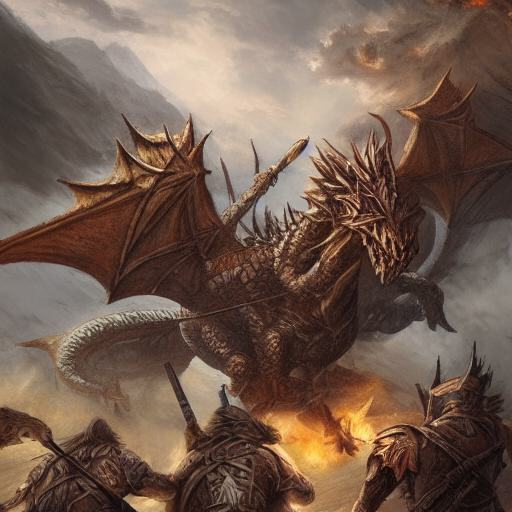
\includegraphics[width=\columnwidth]{introduction/what is a tabletop rpg}
    In tabletop role-playing games like Rise, you play a specific character of your own design.
    Your character can try to do anything you can imagine in a world that the game master, or GM, creates.
    Of course, you won't always succeed.
    The details of your character's capabilities are defined in the pages ahead; when you're done creating a character, it will have a personality of its own, along with strengths, weaknesses, and special abilities.
    Usually, your character will go on adventures with other characters, each of which is played by other players.
    Together, you will create and experience a story with the Game Master, or GM, who defines the universe that the player characters inhabit.

    \subsection{Describing Actions}
        Most of the time, when you're playing a game of Rise, you simply describe what you want your character to do.
        For example, you can say that your character steps out of their room in the inn and walks over to knock on a friend's door.
        Although Rise has rules that could govern some aspects of that scenario, such as an Awareness check to see if your friend notices you knocking, you wouldn't usually reference those rules explicitly.
        Even in the unlikely scenario that your friend doesn't notice you knock the first time, you can just knock again, so there's no point in worrying about the details.
        If something seems reasonable, it probably is, and you don't need to worry about the fiddly bits.

        Sometimes, when you describe what your character tries to do, the action has a narratively relevant chance of failure.
        Instead of knocking on the door to say hi, you might only have time to bang on it once to warn your sleeping friend about an attack from assassins.
        In that case, there's some chance that your friend is sleeping too deeply to notice the noise the first time you knock.
        You could try knocking again, just like in the first scenario, but in this scenario that failure would cost you valuable time to survive the attack.
        In that scenario, you would roll a die to determine whether you succeed in your action - or in this case, whether your friend would succeed in their attempt to notice you.

    \subsection{Using Specific Abilities}
        Instead of describing broadly what you want to have happen, you might choose one of a list of clearly defined abilities that your character can use.
        Every character has specific abilities unique to them, such as a wizard's spells known.
        There are also a number of simple abilities that anyone can use, such as the \ability{dirty trick} or \ability{trip} abilities.
        These universal abilities attempt to adequately describe a wide variety of reasonable improvised actions that you might try to use in combat.

        Explicitly defined abilities have rules for determining what happens when you use them.
        Some abilities, such as attacks in combat, require rolling dice to determine how effective they are.
        Of course, you can use your character's abilities at any time, not just in combat.
        Abilities such as the \spell{create water} or \spell{distant hand} spells can be used to solve other kinds of problems entirely.

    \subsection{Rolling Dice}
        Eventually, you'll have to determine whether something succeeds or fails.
        This can happen as part of using a specific ability that tells you exactly what to roll, or because you tried to narrate your character taking an action that has a dramatically relevant chance of failure.
        In either case, you'll roll a single ten-sided die, also known as 1d10.
        You'll add some modifier that represents how skilled your character is at the particular thing that they are trying to do.
        At the GM's discretion, they may also give the roll an extra bonus or penalty based on the circumstances that your character is in.
        If your die roll is high enough, your character succeeds at whatever they were trying to do.
        Otherwise, your character fails, which may sometimes have additional consequences.

        In Rise, it's entirely possible for characters to be so skilled that they succeed at what they are trying to do even if you roll a 1.
        Likewise, there are tasks that are so obviously impossible for your character that they cannot possibly succeed.
        In those cases, there's no reason to roll!
        Of course, the GM is the final arbiter of whether rolling is necessary.
        They may have information that the players do not.

    \subsection{Why Use So Many Rules?}
        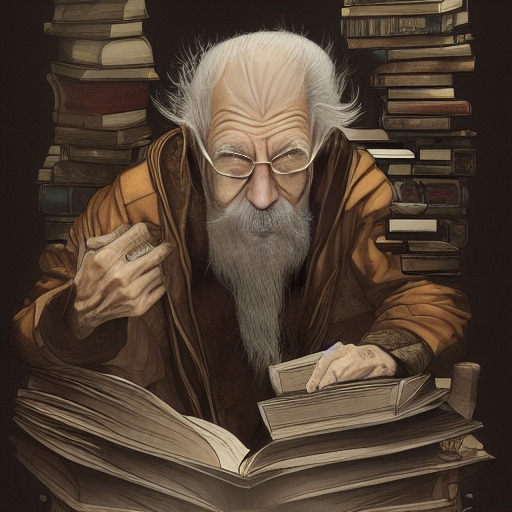
\includegraphics[width=\columnwidth]{introduction/so many rules}

        Tabletop role-playing games attempt to create rules to define how their universe works.
        Some games are intentionally vague or minimalist about their rules, which can be fun!
        Simple games are easy to start playing, and they try to avoid getting in the way of good role-playing.
        However, Rise takes a different approach.
        It spends a lot of effort - and words - attempting to define an internally consistent universe, and creating a large number of specific abilities that can be used in that universe.
        There are a few important advantages to taking this approach: establishing expectations, supporting multiple play styles, and assisting the GM.

        \subsubsection{Establishing Expectations}
            Different people can have very different ideas about what is realistic - or narratively appropriate - in a made-up fantasy universe.
            To some people, kicking in the tavern door and starting a brawl is just some good clean fun, and you'll take a few good punches and then laugh about it later that evening over drinks.
            But to other people, that might sound like a good way to find yourself imprisoned for the foreseeable future with all of your possessions confiscated by the town guard.
            Another interpretation of that scenario might see the brawler seriously injured with a broken bottle in the eye, leaving them partially blinded for weeks - or indefinitely.

            All of those ideas are valid, and they each match the narrative of a particular type of story.
            However, it's important that everyone sitting at a table and playing a game agrees about what to expect.
            Players can get confused or frustrated when their actions have consequences that feel arbitrary or unfair.
            Generally, games are more fun if everyone in the game shares a common set of expectations and conventions.
            Otherwise, games can devolve into disagreements about what is or isn't reasonable.

            One way to establish these expectations is to use a rules system like Rise that defines some expectations explicitly.
            If the scenario above happened in Rise, the last outcome of an incapacitating bottle to the eye shouldn't normally be possible, since the rules explicitly define how injury works.
            Knowing what is and isn't possible can help give players and GMs a useful set of guardrails for what they try to do in the universe.
            It's relatively easy to get everyone to agree about simple things that regular human people have experience with, like how difficult it is to climb a tree.
            However, Rise is full of superhuman people and monsters, and eventually you'll need to figure out how far a barbarian as strong as Hercules can throw a bear.
            Having a single authoritative resource to consult can cut off long disagreements about details that are difficult or impossible to determine objectively.

            Of course, different games played with a flexible rules system like Rise can have very different tones and themes.
            Either of the first two scenarios in the tavern are still plausible in different games, and a GM can use house rules to make vital wounds have more long-term consequences if they want.
            Using a rules system like Rise can help, but it is not the full answer by itself.
            The GM and players always share responsibility for establishing expectations about what genre a game will be, and conforming to those expectations to the extent that it makes the game more fun.

        \subsubsection{Supporting Multiple Play Styles}
            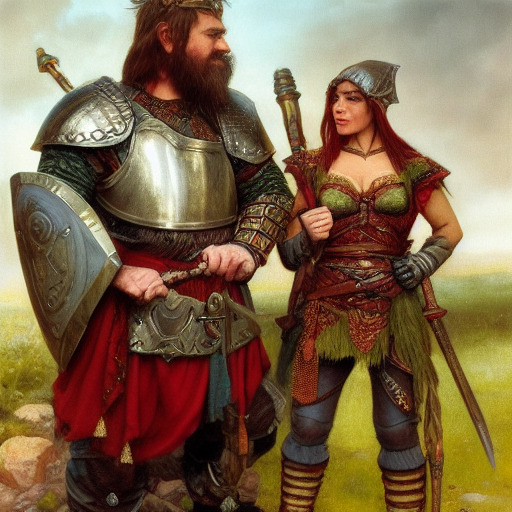
\includegraphics[width=\columnwidth]{introduction/multiple play styles}
            Some people deeply enjoy the process of role-playing itself.
            They enjoy the process of getting into a character and speaking in their voice, exploring their needs and desires, and building a narrative for them over time.
            These people often do not need the confines of a robust rules system, and can play equally well in games with minimal rules or none at all.

            Other people do not enjoy role-playing as an end in itself, or even at all.
            However, they may still enjoy the \textit{game} aspect of a role-playing game.
            Instead of playing a character for their personality and backstory, they may play a character for their unique mechanics and tactical advantages.

            Still other people may be interested in role-playing as a concept, but find it daunting.
            The blank page in front of you when you start painting a picture or writing an essay can be daunting, and that first step is often the hardest to take.
            Giving people a clearly defined set of abilities and specific tools for interacting with the world can enhance creativity by providing a safe space for interaction and experimentation.
            Even if you don't enjoy or feel confident in speaking in your character's voice, you can still engage with the narrative aspects of the adventure by casting a relevant spell or making a relevant skill check.
            People in this middle ground can sometimes enjoy deeper role-playing games while being feeling lost in role-playing games with minimal or nonexistent rules.

            One of the joys - and challenges - of Rise is drawing together people with very different desires and play styles to share a single experience.
            Rules-free role-playing games and tactical wargames can both have a narrower appeal than rules-heavy role-playing games like Rise, which try to provide something for everyone.
            You can run games with deep role-players alongside tactical gamers, and it can be a lot of fun.
            It does place a greater burden on the GM to provide the right ratio of content to keep everyone happy, and it does require the players to be patient when their preferred playstyle is put in the background to support the needs of other players.
            A well-blended game can also draw people out of their comfort zones slowly and safely over time as they observe and start to enjoy the playstyles of the other players in the game.

        \subsubsection{Assisting the GM}
            The Game Master carries an extra weight of responsibility to shape the flow of the game.
            Creating narratively consistent universes, appropriate challenges, and engaging storylines out of thin air is deeply challenging.
            If this job is too difficult, no one will want to do it, and then no one will play the game!
            Making the GM's job easier is a critical component of any role-playing game.

            There are several ways that Rise can make the GM's job easier.
            It provides information about the mechanics and tropes of the universe that the game takes place in, which helps establish expectations and resolve disputes that might come up during the game.
            It will provide a clear narrative foundation for the world and the characters in that world, which minimizes the up-front work required to run a game, once that section of the book is more complete.
            It will provide a wealth of pre-packaged challenges appropriate for players of any power level or play style, and advice for how to use those challenges appropriately, once that section of the book is more complete.
            The GM-focused sections are currently the most unfinished part of Rise, and this will be a more useful guide before Rise is done.

\section{What Makes Rise Different?}
    If you haven't played other tabletop role-playing games, feel free to skip this section.
    If you have, you may wonder what makes Rise unique in a crowded sea of games.
    Rise has five fundamental principles that differentiate it from other TTRPGs: minimal resource management, simultaneous combat, optional complexity, unbounded scaling, and a bounded action economy.

    \subsection{Minimal Resource Management}
        Many games make use of resources like mana, spell slots, or timed cooldowns to limit how often characters can use their abilities.
        These systems have fundamental problems that undercut the fun and flow of a TTRPG, and Rise essentially does not use resources to limit character ability usage.
        In Rise, characters can cast spells or use special attacks any number of times in a row without consuming resources.

        Some systems have resources that are designed to ebb and flow in the course of a typical combat.
        You might expend mana to use a powerful spell, and then regain mana over time by using weaker spells or fulfilling certain conditions.
        Alternately, you might use a spell and then wait some number of in-game turns before you can use that same spell again.
        This can be fiddly to track and hard to recover from if you forget what happened to your resource pool, which is why this approach is more common in video games than in TTRPGs.
        More importantly, this system has no clear way to handle ability usage outside of combat.
        It effectively gives unlimited ability usage when time is no obstacle, but only in an awkward and convoluted way.
        This category of system is unsuitable for Rise because it is too fiddly in combat and doesn't make sense out of combat.

        Some systems have finite-use resources that are tied to the expenditure of in-game time, such as taking long rests, or session breaks.
        You might spend a spell slot to use a powerful spell, and then be unable to cast that spell again until your character rests for some period of time.
        This can be manageable from a complexity perspective if the number of unique resources is small.
        However, it can get dangerously convoluted if characters have a large number of separate or partially interchangeable resource pools, such as using separate pools for individual spell levels.

        The real problem is that this limitation requires you to make your decisions based on not just the current situation, but also on your prediction of all future situations you will encounter before you have the opportunity to rest.
        This contributes significantly to the tactical complexity of deciding each individual action in combat, which slows down the pace of the game.
        It is also punishing to newer players who have less experience with the metagaming required to deduce how many resources an individual fight is worth.
        This strategic complexity is compounded if hit points are treated as an additional resource, since you now have to trade off the potential impact of one limited resource against another limited resource.

        Optimization of resource usage can be unintuitive and out of character, but failure to correctly manage your resources can leave you with no useful abilities remaining.
        This concern can be exacerbated if some characters are extremely resource-intensive while others have no meaningful resources to track.
        No one likes being forced to hide from a difficult fight or take only insignificant actions while your more resource-savvy or resource-independent allies continue using dramatic and powerful abilities.
        It can also add stress to the party dynamics when one character frequently asks for long rests after fights because they expended resources and no one else needs to rest.
        This category of system is unsuitable for Rise because it creates complexity in ways that detract from the fun and narrative of a game instead of adding to it.

        Rise does not use resources to limit normal actions in combat.
        The vast majority of spells, special martial attacks, and other abilities that affect enemies or your environment can be used any number of times.
        There are a small number of abilities with one-round cooldowns, and a universal ability that can only be used once per short rest.
        However, there is no time tracking in the system longer than ``next round''.
        Small cooldowns are a fine-grained balancing tool that allow characters to have powerful abilities which would have detrimental effects for the game if they could be used every turn.

        Rise does use a single universal resource, called ``fatigue'', that recovers based on long rests.
        This allows some opportunity for characters to invest extra effort into specific difficult fights, and to become tired after a long day.
        Normal damage taken during a fight is easily recovered after a ten minute rest.
        This means that you typically don't have to track state between fights.
        However, a GM can prevent that rest time with multiple sequential fights to increase difficulty and drama.

        Overall, Rise uses resource limitations very sparingly.
        This allows it to gain some of their benefits while avoiding the detrimental effects that come from making resource limitations a fundamental part of the system.

    \subsection{Simultaneous Combat}
        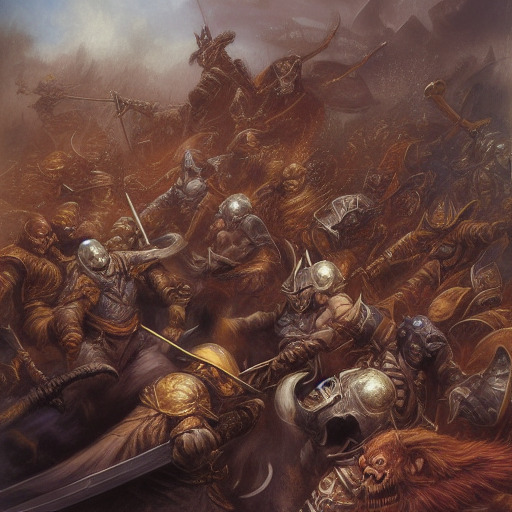
\includegraphics[width=\columnwidth]{introduction/simultaneous combat}
        In most TTRPGs, combat takes place in a series of turns.
        When your turn comes up, you take all of your actions, and then you wait through everyone else's turn until your turn comes again.
        This system has one foundational disadvantage: it is very, very slow.
        Rise uses a simultaneous combat system that dramatically increases the pace of combat.

        Imagine a typical 4-5 player game with 1-2 enemy groups using a traditional turn-based initiative system.
        In this scenario, you have to wait through about 5 turns before it comes back to your turn.
        This number can increase significantly in large-scale fights.
        Each of those 5 or so turns can meaningfully change the battlefield situation on its own by moving, weakening, or defeating various enemies and allies.
        The state of the battlefield at the end of last turn is often drastically different than the state of that battlefield at the start of your new turn.
        Player coordination can be challenging, since they must coordinate in the specific order assigned by the initiative system, and enemy turns can intervene to ruin coordinated plans.

        In theory, every player should accurately track the unfolding battlefield state through each of the intervening turns.
        That would mean everyone would know what to do when their turn comes up.
        In practice, many players find that difficult or impossible.
        Instead, at the start of each of their turns, they ask or try to figure out how the situation has changed.
        Not everyone asks this explicitly, but it must always be analyzed anew.

        Once a player understands the current battlefield state, they can finally decide their actions.
        This typically involves both movement and any number of sequential attacks, so there are many factors to consider.
        Everyone else must wait and do nothing while this happens.
        Once the active player has decided their actions, those actions must be fully rolled and resolved before combat can proceed.
        Even the next player in the initiative order may not be able to make accurate plans during this time, since the die rolls can change those plans.
        All of this combines to make even short combats take an hour or more, and six-person adventuring groups can feel dangerously bloated.

        Rise works differently.
        Combat in Rise is broken up into two phases: the movement phase and the action phase.
        During the movement phase, all creatures move simultaneously, and no attacks are possible.
        Characters can declare certain simple reactive movements like ``stay adjacent to this enemy'' to ensure that they end up in a reasonable position regardless of enemy actions.
        If the movements of characters conflict in impossible ways, initiative checks can temporarily force a linear order of resolution.
        Each player declares their own actions in an arbitrary order as soon as they decide them, so people are not forced to wait and do nothing while slower players contemplate their choices.
        Player coordination is easy, since all actions are happening together.

        During the action phase, players resolve their actions sequentially, but in an arbitrary order of the players' choice.
        This allows slower players to make their decisions when they are ready, while allowing faster players to resolve their actions first.
        Since movement during the action phase is rare, and enemies cannot unexpectedly move, players are typically able to decide their actions much more quickly and easily even when they have a large number of unique abilities to choose from.
        Once all players have resolved their actions, they learn what their enemies did.
        Those actions all resolve simultaneously, so enemy actions cannot interrupt player actions and vice versa.
        Attackers are always responsible for rolling instead of using ``saving throws'' or similar mechanics that force defenders to roll dice.
        All of this means that players can choose and resolve their actions simultaneously and efficiently, minimizing total time spent in combat while still allowing significant tactical complexity.

        The start of each phase still requires a general assessment from all acting players about the current state of the battlefield, which takes just as much time as the assessment in a classic initiative system.
        However, the time required for this tactical analysis only increases marginally as the number of players and enemies in the game increases.
        This allows Rise to handle large player counts or large enemy hordes without becoming glacially slow.
        Combat in Rise flows by quickly, making it much easier to balance time between combat and non-combat encounters within the same game session - or to run through multiple separate, individually challenging combats without sacrificing the pace and energy of the game.

    \subsection{Optional Complexity}
        Many games operate at a consistent level of complexity.
        Many rules-light games are always simple, and many rules-dense games are always complex.
        This is a perfectly reasonable design philosophy.
        Among other benefits, it makes it easy to know what to expect from the game, which helps give the game a well-defined niche.

        Rise is designed to allow players to choose their own level of complexity.
        This broadens its potential audience by allowing people with very different play styles or tolerances for complexity to enjoy the same game together.
        This goal is manifested in several key ways in Rise's design:
        \begin{itemize}
            \item Core gameplay is designed to be simple.
            \item Character creation is deeply interconnected.
            \item Complexity is not tied to narrative roles.
            \item Character power does not require complexity.
        \end{itemize}

        \subsubsection{Simple Core Gameplay}
            The core gameplay loop must be simple.
            You can contribute in combat by relying on one or two standard attacks that you use in all circumstances.
            In narrative situations, you can just roll the skills you have trained, and ignore other options.
            Engaging with the system more deeply than that is a choice, not a requirement.

        \subsubsection{Interconnected Character Creation}
            Character creation and build optimization is a better place to store complexity.
            Creating a Rise character involves a number of decisions, each of which can have nuanced ramifications on other aspects of the system.
            If you are just trying to build a character that matches a desired narrative, you can generally approach each decision in isolation.

            For example, you can decide that your character is intelligent and agile but not very strong or durable, because that is the concept you want.
            That decision has consequences, such as changing how many trained skills you have and what your defenses are.
            If you approach each decision sequentially, each one is relatively easy to make, and doesn't require deep system knowledge.
            On the other hand, trying to mathematically optimize a character requires thinking about many aspects of the system at once.
            This results in a system that is easy to learn but hard to master.

            Even for simple characters, the process of character creation is still one of the most complicated aspects of Rise.
            That is why Rise provides (or will provide, once that section is done) an extensive selection of premade characters for a wide variety of narrative archetypes.
            Each premade character includes advice for how to play that character and level them up.
            The premade characters make the system more accessible to people who don't want to to deal with the complexity of creating a character from scratch.

        \subsubsection{Complexity and Narrative}
            Complexity and simplicity should not be directly connected to a character's concept or narrative.`
            For example, it would be a bad idea to define a system where martial characters are simple and spellcasters are complicated.
            Both of those are rich and evocative narrative constructs.
            Many people who don't enjoy complexity will want to play spellcasters, and many people who enjoy complexity will want to play martial characters.
            Gameplay complexity must be more finely tuned and localized than those sweeping strokes.

            In Rise, gameplay complexity is generally generated by acquiring a large number of increasingly situational abilities.
            Every class has some archetypes that grant additional abilities known and some archetypes that grant additional passive abilities.
            If you like having a lot of unique abilities, you can have a high Intelligence to maximize your insight points, and focus on learning spells and maneuvers that attack your enemies or have situational effects.
            If you like minimizing complexity, you can instead choose archetypes or learn spells that simply grant you passive benefits, and focus on one or two standard attacks that you specialize in.
            Some feats give you new abilities and new circumstances to pay attention to that make you more effective, while others simply increase your passive statistics and defenses.

            Rise specifically handles complexity for martial characters and spellcasters slightly differently.
            Martial characters in Rise typically have fairly simple individual abilities.
            However, they can use those abilities with a variety of meaningfully different weapons.
            A martial character with four unique attacks and three different weapons has twelve different options in combat.
            In addition, martial characters can typically make better use of universal abilities, such as shoving and grappling.

            Spellcasters have more complex and varied individual abilities.
            They also tend to have more abilities that have significant narrative effects.
            However, their abilities are more isolated.
            There is no spellcaster equivalent of martial weapons that would multiply their number of distinct abilities in combat.
            The result of this design is that both martial characters and spellcasters can be very simple or very complicated.
            However, they approach complexity in different ways, ensuring that they feel narratively distinct.

        \subsubsection{Complexity and Power}
            All of this customization of complexity would be mostly pointless if complexity was strongly correlated with character power.
            If exceptionally complicated or hyper-specialized characters were obviously and consistently more effective than other characters, it would push everyone to use those characters.
            Rise structures the tradeoffs between gaining raw power and gaining additional options balanced enough that neither is always superior.

            There will always be some benefit from build optimization and system mastery.
            Players who are deeply familiar with Rise will be able to build characters with more relevant strengths and fewer relevant weaknesses.
            However, the gap between optimized characters and ``normal'' characters is limited.
            There will always be specific contexts where one character's mechanics are superior to another's.
            For example, a specialized defensive melee character may excel in a duel in a confined space.
            However, it may be irrelevant against cavalry archers on an open field.
            Characters in Rise cannot drastically change their capabilities each day, so they will always have moments to shine and moments of weakness.

    \subsection{Unbounded Scaling}
        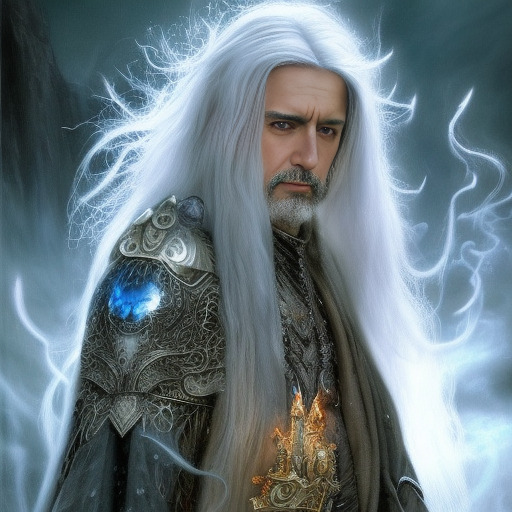
\includegraphics[width=\columnwidth]{introduction/unbounded scaling}
        Some systems uses bounded bonuses for accuracy or other game statistics.
        Bounded scaling means that every character of the same power level - or in some systems, of any power level - has a similar chance of success with any given skill check or attack roll.
        This can frequently cause narratively inappropriate and even comical events, and Rise explicitly rejects this philosophy.

        Imagine a typical party of four players, with one character being exceptionally skilled at a particular task.
        Perhaps the rogue is exceptionally skilled at lying, or a barbarian is exceptionally skilled at climbing.
        If ``exceptionally skilled'' only means that they have a \plus5 bonus on a d20 compared to \plus0 from the rest of the party, the exceptionally skilled character will only get the best result in the party half the time.
        The other half of the time, some other character with no relevant skills will meet or exceed the skilled character's result - sometimes by a dramatic margin.
        When failure compared to rank amateurs happens this often, it becomes hard to take seriously the idea that any character can be exceptionally skilled at anything.

        Rise characters can have dramatic statistical differences between each other, even at low levels.
        It uses a d10 as the fundamental die, which makes every bonus more significant.
        In addition, a 1st-level character can easily reach a \plus6 bonus with a skill check that is particularly relevant to their character.
        This means that a skilled character can beat a party of rank amateurs 80\% of the time, and at higher levels their success becomes completely guaranteed.
        Likewise, the difference in Mental defense between a powerful sorcerer and a cowardly rogue can allow mind-affecting attacks to almost always hit a rogue while almost never hitting the sorcerer.
        These statistical differences do not always grow with level, but they remain significant at every level.

        One advantage of systems with bounded scaling is that it is easier to guarantee that every character is relevant in any situation.
        Even if your character has no useful abilities of any kind, you might sometimes succeed on important actions through sheer luck.
        However, this design philosophy often breaks the symmetry between magical and non-magical characters.
        Magical characters can often use extremely specific and powerful abilities that are impossible for nonmagical characters to duplicate.
        If magical characters also have similar odds of success with all generic mechanics of the game, they will almost certainly have far more influence over the narrative of the game than any nonmagical character can hope to match.

        The philosophy of Rise is that it's okay for some characters to be irrelevant in specific contexts.
        It's good to give people time in the spotlight where their character's abilities help solve the specific problem that the group is facing when no other character could.
        Rise encourages that, and makes it impossible for one character to be relevant in \textit{all} contexts.
        Each character has their own strengths and weaknesses, and if you try to be good at everything, you'll fall behind people who specialize in a particular area.
        This will naturally rotate the spotlight between different characters, allowing each player to feel relevant and important in turn.

        This dramatic scaling is also used to govern the power of characters over time, in addition to the power of characters relative to each other.
        Rise attempts to model a massive power range for player characters.
        They are expected to start their journeys at level 1 as little more than commoners, and by level 21 they are effectively demigods who can alter the fate of entire worlds.
        This is a critical part of the narrative fabric of Rise, and it is reflected in the statistics and abilities of characters.
        If a level 1 kobold posed even a tiny threat to a level 21 character, the mechanics of the game would sabotage the purported narrative of power and growth.
        In Rise, overall character power doubles approximately every two to three levels.
        The system takes some care to avoid bloating numbers to unwieldy levels on this journey, and the use of the d10 as the standard die helps immensely.

    \subsection{Bounded Action Economy}
        It is dangerous to to give characters too many actions each turn.
        Each additional action a character can take increases how difficult it is for a player to decide what to do on their turn.
        In addition, each additional action increases the complexity of the change between the start of the turn and the end of the turn.
        This is especially risky with Rise's simultaneous initiative system, which combines the actions taken by all characters into a single resolution process.

        Rise places significant limitations on how many relevant actions each character can take on their turn.
        Generally, characters can only move during the movement phase and then take one significant action each turn.
        Some characters can use a minor action to accomplish something useful.
        However, that essentially marks the end of action economy scaling, even up to the maximum level.

        Detrimental effects that could deny actions are also heavily limited.
        Total action denial effects are only usable by high level characters, and even then they only work against weak enemies or enemies that have already been significantly damaged.
        Taking actions is fun, and sitting quietly while everyone else does things can be very frustrating.
        Similarly, completely removing an enemy's ability to act can easily remove the tension from a fight before it's actually over.

\chapter{Basic Mechanics}

\section{Attributes}
Each character has six \glossterm[attribute]{attributes}: Strength (Str), Dexterity (Dex), Constitution (Con), Intelligence (Int), Perception (Per), and Willpower (Wil).
Each attribute represents a character's raw talent in that area.
A 0 in an attribute represents average human capacity.
That doesn't mean that every commoner has a 0 in every attribute; not everyone is average, after all.

\subsection{Attribute Descriptions}

\subsubsection{Strength (Str)}\label{Strength}
Strength measures muscle and physical power.
\begin{itemize}
    \item Strength determines how much a character can carry, as described in \tref{Weight Limits}.
    \item Strength can be used to attack with melee and thrown weapons.
    \item Strength can be used to deal damage with all physical attacks.
    \item Strength can be used for Maneuver and Fortitude defenses.
    \item Strength can be used for Climb, Jump, Sprint, and Swim checks.
    \item For every 5 Strength you have, you gain a \plus1 bonus to damage with physical attacks. If your Strength is negative, you take a penalty to damage with physical attacks equal to half your Strength.
\end{itemize}

\subsubsection{Dexterity (Dex)}\label{Dexterity}
Dexterity measures hand-eye coordination, agility, and reflexes.
\begin{itemize}
    \item Dexterity can be used to attack with light melee and thrown weapons.
    \item Dexterity can be used for all physical defenses (Armor, Maneuver, and Reflex).
    \item Dexterity can be used for Balance, Escape Artist, Ride, Sleight of Hand, Stealth, and Tumble checks.
    \item For every 5 Dexterity you have, you gain a \plus1 bonus to physical defenses (Armor, Maneuver, Reflex). If your Dexterity is negative, you take a penalty to your physical defenses equal to half your Dexterity.
\end{itemize}

\subsubsection{Constitution (Con)}\label{Constitution}
Constitution represents your character's health and stamina.
\begin{itemize}
    \item Constitution can be used for Armor and Fortitude defenses.
    \item For every 2 Constitution you have, you gain a \plus1 bonus to Fortitude defense. If your Constitution is negative, you take a penalty to Fortitude defense equal to your Constitution.
\end{itemize}

\subsubsection{Intelligence (Int)}\label{Intelligence}
Intelligence determines how well your character learns and reasons.
It affects your character's knowledge in many areas.

\begin{itemize}
    \item Intelligence is added to Craft, Disguise, Heal, Knowledge, and Linguistics checks.
    \item Intelligence can be used for to Mental defense.
    \item You gain bonus languages on character creation equal to your starting Intelligence.
    \item For every 2 Intelligence you have, you gain an extra skill point. If your Intelligence is negative, you take a penalty to your skill points equal to your Intelligence.
\end{itemize}

\par An animal has an Intelligence score of \minus6 or lower.
A creature of humanlike intelligence has a score of at least a \minus5 Intelligence.

\subsubsection{Perception (Per)}\label{Perception}
Perception describes a character's ability to observe and be aware of one's surroundings.
\begin{itemize}
    \item Perception can be used to attack with projectile weapons.
    \item Perception can be used for Awareness, Creature Handling, Sense Motive, Spellcraft, and Survival checks.
    \item Perception can be used for Reflex defense.
    \item For every 5 Perception you have, you gain a \plus1 bonus to accuracy with physical attacks. If your Perception is negative, you take a penalty to accuracy with physical attacks equal to half your Perception.
\end{itemize}

\subsubsection{Willpower (Wil)}\label{Willpower}
Willpower measures a character's ability to endure mental hardships.
\begin{itemize}
    \item Willpower can be used for Mental defense.
    \item Many special abilities are based on Willpower.
    \item For every 5 Willpower you have, you gain a \plus1 bonus to Mental defense. If your Willpower is negative, you take a penalty to Mental defense equal to your Willpower.
\end{itemize}

\subsection{Using Attributes}

\subsubsection{Choosing Attributes to Use}
In many cases, multiple attributes can be used for the same thing.
For example, both Strength and Dexterity can be used to attack with light weapons such as daggers.
Whenever more than one attribute could be used, you must choose which one to use (usually, the higher attribute).

\subsection{Determining Attributes}
There are several options for how to determine attribute scores.

\subsubsection{Predefined Attribute Scores}
This is the simplest method.
Simply take the following set of attribute scores and distribute them as you choose among your character's abilities:

4, 3, 2, 1, 0, \minus1

This set of attribute scores is called the ``elite array''.
For more extreme characters, you may use the ``savant array'':

5, 2, 1, 0, 0, \minus2.

Finally, for more well-balanced characters, you may use the ``balanced array'':

3, 3, 2, 1, 1, 0

\subsubsection{Point Buy}
With this method, you can fully control your character's attribute scores to match what you want your character to be.
All your character's attribute scores start at 0.
You get 10 points to distribute among your character's attribute scores.
Attribute scores can be bought according to the costs on \trefnp{Attribute Score Point Costs}.

\begin{dtable}
    \lcaption{Attribute Score Point Costs}
    \begin{dtabularx}{\columnwidth}{X X}
        \tb{Attribute Score} & \tb{Point Cost} \\
        \hline
        \minus2 & \minus2\fn{1} \\
        \minus1 & \minus1\fn{1} \\
        0       & 0             \\
        1       & 1             \\
        2       & 2             \\
        3       & 3             \\
        4       & 5             \\
        5       & 8             \\
    \end{dtabularx}
    1 No more than two attribute scores can be reduced below 0 in this way.
\end{dtable}

\subsection{Changing Attributes}

Your attributes increase as you gain levels (see \pcref{Character Advancement}), and some special abilities can also increase your attributes, either permanently or for a brief period of time.
When an attribute changes, abilities and modifiers based on the attribute change at different times, as shown on \trefnp{Effects of Changing Attributes}.

\begin{dtable*}
    \lcaption{Effects of Changing Attributes}
    \begin{dtabularx}{\textwidth}{l >{\lcol}p{10em} X}
        \tb{Effect Type} & \tb{Timing of Change} & \tb{Example} \\
        \hline
        Numerical modifiers   & Immediately & A barbarian enters a rage.  His physical damage increases immediately.  \\
        Ability prerequisites & Immediately & A paladin's Strength is drained by a ghost.  She loses the benefits of her Power Attack feat immediately.  \\
        Ability use limits    & When ability uses are regained & A fighter puts on a magic item that grants additional Willpower.  He gains additional daily uses of his combat discipline ability after resting for the night.  \\
        Hit points            & On level up\fn{1} & A druid casts \spell{totemic power} to increase his Constitution. His hit points do not change. \\
        Skill points          & On level up\fn{1} & A wizard reads an ancient magical tome that increases her Intelligence. Her skill points increase when she gains a level. \\
    \end{dtabularx}
    1. Hit points and skill points are not normally affected by spells, worn magic items, or other temporary effects.
\end{dtable*}

\section{Combat Overview}\label{Combat Overview}

Combat takes place in a series of ``rounds'', which represent about six seconds of action.
In combat, creatures attack each other (see \pcref{Attacks}) and defend themselves (see \pcref{Defenses}), while moving around the battlefield (see \pcref{Movement and Positioning}).
When your defenses fail, you can get hurt (see \pcref{Injury, Death, and Healing}).
In unusual situations, you might become more or less likely to succeed at your actions (see \pcref{Circumstances, Bonuses, and Penalties}).

\subsection{Combat Phases}

Each round of a combat is divided into two phases: a movement phase and an action phase.
During each phase, all characters declare their actions simultaneously, and then those actions are resolved simultaneously.
After both phases are complete, the round ends.

\subsubsection{The Movement Phase}\label{The Movement Phase}

The movement phase takes place first in the round.
During the movement phase, all creatures can move a distance equal to their speed (see \pcref{Movement and Positioning}).
In addition to moving, creatures can take minor actions that require motion, such as drawing a weapon.
These actions are called \glossterm{move actions}.

You can take any number of move actions during the movement phase, as long as all of those actions can be performed simultaneously.
For example, you can walk your speed and draw your sword in a single movement phase.
However, you cannot draw a sword and equip a shield in the same phase.
Equipping a shield takes two hands, leaving you with no free hand to draw your sword.

Once all creatures are done moving, the action phase begins.

\subsubsection{The Action Phase}\label{The Action Phase}

During the action phase, each creature can take a single \glossterm{standard action}.

\parhead{Standard Action} You can use a standard action to attack with a weapon, cast a spell, drink a potion, and do most other things that take concentration and effort.

\subsection{Resolving Actions}\label{Resolving Actions}

Within each phase, actions of all creatures are simultaneously resolved in the following order.

\begin{enumerate*}
    \item Choose actions.
    \item Determine affected targets.
    \item \textit{Resolve swift actions}.
    \item Check action success.
        Example: Making attack rolls.
    \item Determine action results.
        Example: Making damage rolls.
    \item Apply non-spell action results.
        Examples: Reducing hit points, moving character locations, and applying penalties.
    \item \textit{Make Concentration checks to maintain focus on spells}.
    \item Apply spell results.
\end{enumerate*}

In the vast majority of cases, there is no need to go through this order explicitly.
Combats will run much faster if attack and damage rolls are generally made and announced at the same time as the actions are chosen, even before all characters have explicitly stated their actions.
The order of resolution matters when creatures take actions that directly conflict with each other.

\subsubsection{Conflicting Actions}\label{Conflicting Actions}

Sometimes, actions that occur within the same resolution step can conflict with each other.
There are two main methods for resolving these conflicts.

\parhead{Mutually Exclusive Actions} Sometimes, actions that should take place at the same time directly conflict with each other.
This most commonly happens when two creatures move to the same place.
In this case, each involved character rolls initiative.
The creature with the highest initiative result succeeds.
All other creatures come as close as possible to completing their intended action.

Your initiative check is calculated as follows:

\begin{figure}[h]
    \centering Dexterity or Perception \add other bonuses and penalties
\end{figure}

For example, if two creatures were racing to reach a door, they would both roll initiative.
The winner would reach the door and stop in their intended square, and the loser would stop adjacent to their intended square.

\parhead{Conditionally Impossible Actions} In rare cases, one action may make another action impossible if the first action succeeds.
However, unlike with mutually exclusive actions, the second action would not make the first action impossible.
This usually happens if a creature moves during the action phase while being attacked.
If the attack trips or deals enough damage to kill the moving creature, its movement becomes impossible.
In this case, the second action is negated, and the creature takes no action during that action phase.

\subsection{Special Actions}

\parhead{Swift and Immediate Actions}\label{Swift and Immediate Actions} Each round, you can take a single swift or immediate action.
Swift and immediate actions can be taken in either the movement or action phase.
Swift actions must be declared along with any other actions you intend to take during that phase.
Immediate actions do not need to be declared ahead of time.
Instead, abilities that can be used as immediate actions specify triggering conditions that allow the action to be taken.

Swift and immediate actions are resolved early in the phase, before other actions resolve.
If multiple swift or immediate actions are taken simultaneously, they are resolved using the normal rules for resolving simultaneous actions.

\parhead{Full-Round Actions} A full-round action requires your character's full attention.
Most full-round actions involve a combination of movement and concentrated effort, such as charging to strike a distant foe or running at full speed.
Unless otherwise specified, you perform any movement required for the action during the movement phase, and the rest of the action during the action phase.

\parhead{Delaying}\label{Delaying}
During a phase, you can delay your action instead of acting immediately.
If you delay, you do nothing until after the actions of all other creatures have been resolved.
At that point, you can choose to continue delaying in the next phase, or you can declare and resolve an action.
If multiple creatures delay, all their actions are declared and resolved in the normal action resolution order, as if they were part of a shared ``delay phase''.
After taking a delayed action, you do not act during the next phase.

For example, if you delay during the movement phase, you can move after all other actions have been declared and resolved.
You can continue delaying to see what actions are taken during the action phase.
At the end of the action phase, you could take actions for your own ``action phase''.
In exchange, you would skip the following movement phase, and could only act again during the next action phase.

\subsection{Attacks}\label{Attacks}
An \glossterm{attack} is anything that affects another creatures in a potentially harmful way.
There are two kinds of attacks: physical attacks, which are made with weapons or fists, and special attacks, which are made with magic or supernatural power.
All physical attacks, and most special attacks, require making an \glossterm{attack roll} against a \glossterm{defense}.
To make an attack roll, you roll 1d20, adding your \glossterm{accuracy} with the attack to the roll.
If the result of the attack roll equals or exceeds the defense, the attack succeeds.

\subsubsection{Standard Attack}\label{Standard Attack}
As a standard action, you can make a single \glossterm{strike} with a weapon you are wielding against an enemy.
If you're using a melee weapon, you must \glossterm{threaten} your target.
If you're using a ranged weapon, the target must be within the weapon's maximum \glossterm{range}.

To make a strike, make an attack roll, as with most other atacks.
If your attack roll beats the target's Armor defense, your foe takes damage.

\subsubsection{Accuracy}
Your accuracy with physical attacks is equal to the following:

\begin{figure}[h]
    \centering Combat prowess or attack attribute \add proficiency bonus \add size modifier \add other bonuses and penalties
\end{figure}

\parhead{Attack Attribute} You can use Strength to attack with melee and thrown weapons, Dexterity to attack with melee and thrown weapons that are light, and Perception to attack with projectile weapons.
\parhead{Proficiency Bonus} You gain a \plus4 bonus to accuracy with a weapon you are proficient with.
\parhead{Size Modifier} Your size modifier is described in \tref{Size in Combat}.

\subsubsection{Damage}
If your strike hits, you deal damage equal to your weapon's damage die \add half your combat prowess or half your Strength.

\parhead{Dealing Nonlethal Damage} You can attempt to strike nonlethally with any weapon.
If you hit, you deal half damage as \glossterm{nonlethal damage} (see \pcref{Nonlethal Damage}).

\subsubsection{Reach}\label{Reach}
Normally, you can make melee attacks against anyone within five feet of you.
The range at which you can make melee attacks is called your \glossterm{reach}, and the area that you can attack into is called your \glossterm{threatened area}.
Reach for larger and smaller creatures is determined by size, as shown on \trefnp{Size in Combat}.

\subsection{Defenses}\label{Defenses}
Usually, when you are attacked, the attacker has to make an attack roll against a specific defense.
If the attack roll is at least as high as that defense, the attack succeeds.
There are three physical defenses and two special defenses.
\begin{itemize}
    \item Armor defense (AD): Your Armor defense protects you from normal physical attacks, such as attempts to hit you with a sword.
        It is the most commonly used defense.
        Armor defense is a physical defense.
    \item Maneuver defense: Your Maneuver defense protects you from unusual physical attacks, such as attempts to trip or disarm you.
        Maneuver defense is a physical defense.
    \item Reflex defense: Your Reflex protects you from attacks you have to avoid, such as explosions or falling rocks.
        Reflex defense is a physical defense.
    \item Fortitude defense: Your Fortitude defense protects you from attacks you have to physically endure or resist, such as poisons and deadly spells.
        Fortitude defense is a special defense.
    \item Mental defense: Your Mental defense protects you from attacks you have to mentally endure or resist, such as terrifying creatures and magical manipulation.
        Mental defense is a special defense.
\end{itemize}

\subsubsection{Defense Values}

Each of your defenses is calculated in the following way:

\begin{figure}[h]
    \centering 10 \add Base defense bonus or defense attribute(s) \add size modifier \add other bonuses and penalties
\end{figure}

The attributes and relevant bonuses which apply to each defense are described in \trefnp{Defense Calculations}.

\begin{dtable!*}
    \lcaption{Defense Calculations}
    \begin{dtabularx}{\textwidth}{l l l l l >{\lcol}X}
        \tb{Defense Name} & \tb{Defense Bonus} & \tb{Attributes} & \tb{Body Armor Modifier} & \tb{Shield Modifier} & \tb{Size Modifier} \\
        \hline
        Armor defense     & Combat prowess    & Dex or Con        & Yes & Yes & Yes     \\
        Maneuver defense  & Combat prowess    & Str or Dex        & No  & Yes & Special \\
        Fortitude defense & Base Fortitude bonus & Con \add half Str & No  & No  & No      \\
        Reflex defense    & Base Reflex bonus    & Dex \add half Per & No  & Yes & Yes     \\
        Mental defense    & Base Mental bonus    & Wil \add half Int & No  & No  & No      \\
    \end{dtabularx}
\end{dtable!*}

\parhead{Natural Armor} Creatures with unusually tough skin or thick hide, including most monsters, gain bonuses to their Armor defense.
These bonuses stack with any armor such creatures might wear.
\parhead{Size Modifiers} Your size modifier and special size modifier are described on \tref{Size in Combat}.

\subsection{Movement and Positioning}\label{Movement and Positioning}

\subsubsection{Taking up Space}
A typical human takes up a 5-ft. by 5-ft.  space in combat.
For convenience, this is often called a \glossterm{square}.
Differently sized creatures can take up more or less space, as indicated on \tref{Size in Combat}.
Normally, other creatures can't be in any squares you occupy.

Sometimes, movement and distance are represented in squares.
A 30-ft. movement is the same thing as moving six squares.

\subsubsection{Moving}

When you move, you can travel a number of feet up to your speed in any direction.
For simplicity, all movement is measured in five-foot increments.
While it is possible to be more precise than that, it's generally not worth the complexity.

\subsubsection{Measuring Movement}

\parhead{Diagonals} When measuring distance, the first diagonal counts as five feet of movement, and the second counds as ten feet of movement.
The third costs five feet, the fourth costs ten feet, and so on.
You can move diagonally past corners and enemies.

\subsubsection{Threatening Foes}
All squares threatened by any foes cost double the normal movement cost to move out of.

\subsection{Injury, Death, and Healing}\label{Injury, Death, and Healing}

\subsubsection{Hit Points}\label{Hit Points}
Your hit points measure how hard you are to kill.
No matter how many hit points you lose, your character isn't significantly hindered until your hit points drop to 0.
When you run out of hit points, your actions are limited and you might die.

Your hit points are equal to your \term{hit value} \mtimes your level.
Your hit value is calculated as follows:

\begin{figure}[h]
    \centering Half Fortitude defense or half Mental defense \add other bonuses or penalties
\end{figure}

\parhead{Temporary Modifiers} Temporary effects which alter your Fortitude or Mental defenses, including changes to your Constitution or Willpower, do not alter your maximum or current hit points.
Your maximum number of hit points is determined when you gain a level, and generally does not change between levels.
Some effects specifically modify your maximum hit points, such as the \spell{curse of blood and bone} spell.

\subsubsection{Losing Hit Points}
When you take lethal damage, you subtract that damage from your hit points.
\parhead{What Hit Points Represent} Hit points represent a combination of durability, luck, divine providence, and sheer determination, depending on the nature of your character.
When you take 10 damage from an orc with a greataxe, the axe did not literally carve into your skin without affecting your ability to fight.
Instead, you avoided the worst of the blow, but it bruised you through your armor, the effort to dodge the blow fatigued your character, or it barely nicked you through sheer luck -- and everyone's luck runs out eventually.

\subsubsection{Critical Damage}\label{Critical Damage}
When you take damage while you are disabled (see \pcref{Disabled}), that damage represents serious physical injury to your body.
This is called critical damage.
You suffer a penalty to accuracy, checks, and defenses equal to the amount of critical damage you have.

While you have critical damage, magical healing which would normally restore hit points cannot restore your hit points, though it can stabilize you, preventing you from dying.
In addition, if you take damage that would reduce your hit points to 0 while you have any critical damage, any excess damage from the attack is dealt directly as critical damage.

\subsubsection{Overkill Damage}
Normally, when you take damage that would reduce your hit points to 0, any excess damage from the attack is wasted.
However, some attacks deal such massive damage that you begin dying immediately, rather than just becoming staggered.
If the damage dealt by an attack exceeds your maximum hit points (not current hit points), any damage past what would reduce your hit points to 0 is dealt as critical damage rather than being wasted.

\subsubsection{Stages of Injury}

\parhead{Healthy} When you are above half hit points, you suffer no significant effects from losing hit points.
If you take damage, you can become bloodied (see Bloodied, below).

\parhead{Bloodied} When you drop to half your hit points or below, you are \bloodied.
If you take additional damage, you can become disabled (see Disabled, below).

\parhead{Disabled}\label{Disabled} At the end of each round, if you have no hit points remaining after resolving all other effects in the round, you become disabled.
While disabled, you are both \staggered and bloodied.

At the end of the round, after all other effects have been resolved, if your hit point total is positive, you stop being disabled.
If you take additional damage while disabled, that damage is critical damage and causes you to begin dying (see Dying, below).

\parhead{Dying}\label{Dying} While you are dying, you must make an attack against your own Fortitude defense at the end of every round.
No bonuses or penalties apply to the attack roll, but \glossterm{critical damage} can penalize your Fortitude defense.
If this attack succeeds once, you fall unconscious.
If it succeeds three times, you die.
If this attack fails three times, you stabilize.

If you receive magical healing of any kind while dying, you become partially stabilized.
While partially stabilized, you must make an attack against your Fortitude once per minute, instead of once per round.

An ally can make a Heal check to tend to you while you are dying.
The Heal check result can be used in place of your Fortitude defense, although the critical damage you have taken applies as a penalty to the Heal check result as well.

\parhead{Stable}\label{Stable}
If you have taken critical damage but managed to stave off death, you become stable.
As long as you have critical damage, magical healing has no effect on your hit points, though some magical effects can heal critical damage.
If you became unconscious while dying, you regain consciousness as soon as you have hit points.

\subsubsection{Healing}
After taking damage, you can recover hit points through natural healing or through magical healing.
In any case, you can't regain hit points past your full normal hit point total.

\parhead{Natural Healing} With 8 hours of rest, you recover half your hit points.
Any significant interruption (such as combat or the like) during your rest prevents you from healing.
If you rest for an entire day (16 hours), you recover all your hit points.

\parhead{Magical Healing} Various abilities and spells can restore hit points.
However, only certain spells can heal critical damage, as specified in the spell description.
Unless a spell says it can cure critical damage, it cannot -- though it can still stabilize dying characters.
Magical healing has no effect on the hit points of creatures with critical damage.

\parhead{Healing Ability Damage} Ability damage is temporary, just as hit point damage is.
Ability damage returns at the rate of 1 point per 8 hours of rest for each affected attribute score.

\parhead{Healing While Disabled} While you are disabled, any healing you receive cancels out damage you receive in the same phase on a one-for-one basis.
This can prevent you from taking critical damage if you are damaged while disabled.

\parhead{Healing Critical Damage} Critical damage takes much longer to heal than hit point damage.
Resting for 1 week restores an amount of critical damage equal to 1 \add half the character's Constitution (minimum 1).
A character can have both hit points and critical damage.
As long as a character has critical damage, he is staggered, even if he is at full hit points.

\subsubsection{Nonlethal Damage}\label{Nonlethal Damage}
Some attacks and environmental effects deal nonlethal damage.
Nonlethal damage is not subtracted from your hit points.
Instead, it is tracked separately.
If your nonlethal damage exceeds your hit points, you become staggered, just as if you were at 0 hit points.
If you take additional damage while staggered, you fall unconscious.
However, you do not begin dying unless your hit points are actually below 0.

\parhead{Healing Nonlethal Damage}
You heal half your hit points in nonlethal damage with 1 hour of rest.
When a spell or a magical ability cures hit point damage, it also removes an equal amount of nonlethal damage.

\subsection{Temporary Hit Points}\label{Temporary Hit Points}
Certain effects give a character temporary hit points which act as a protection against damage.
Whenever a character takes damage, if he has temporary hit points, the damage is applied to his temporary hit points first.
Any excess damage is then applied to his hit points as normal.
Temporary hit points are not ``real'' hit points, and cannot be healed.
If a character has temporary hit points from multiple effects, only the highest value is used.

\subsection{Circumstances, Bonuses, and Penalties}

\subsubsection{Overwhelm}\label{Overwhelm}
When a creature is being attacked by multiple foes at once, it is less able to defend itself.
A creature is considered overwhelmed if it is being threatened by more than one creature.
Multiple creatures occupying the same square count as a single creature when determining overwhelm penalties.
If a creature is overwhelmed, it takes a penalty to physical defenses equal to the number of creatures threatening it.

\subsubsection{Range Increments}
When using a ranged weapon, you take a \minus2 penalty per range increment between you and your target.
For example, when using a longbow with a range increment of 100 feet against a target 170 feet away, you take a \minus2 penalty to accuracy.

\subsubsection{Size in Combat}\label{Size in Combat}
Size affects your space and reach in combat.
In addition, your physical attacks and defefenses are affected by your size modifier.
These effects are shown on \trefnp{Size in Combat}.

\begin{dtable*}
    \lcaption{Size in Combat}
    \begin{dtabularx}{\textwidth}{l l l l l X}
        \tb{Size} & \tb{Space\fn{1}} & \tb{Reach\fn{1}} & \tb{Size Modifier\fn{2}} & \tb{Special Size Modifier\fn{3}} & \tb{Example Creature} \\
        \hline
        Fine              & 1/2 ft.    & 0          & \plus8  & \minus16 & Fly                      \\
        Diminutive        & 1 ft.      & 0          & \plus4  & \minus12 & Toad                     \\
        Tiny              & 2-1/2 ft.  & 0          & \plus2  & \minus8  & Cat                      \\
        Small             & 5 ft.      & 5 ft.      & \plus1  & \minus4  & Halfling                 \\
        Medium            & 5 ft.      & 5 ft.      & \plus0  & \plus0   & Human                    \\
        Large (tall)      & 10 ft.     & 10 ft.     & \minus1 & \plus4   & Ogre                     \\
        Large (long)      & 10 ft.     & 5 ft.      & \minus1 & \plus4   & Horse                    \\
        Huge (tall)       & 15 ft.     & 15 ft.     & \minus2 & \plus8   & Cloud giant              \\
        Huge (long)       & 15 ft.     & 10 ft.     & \minus2 & \plus8   & Bulette                  \\
        Gargantuan (tall) & 20 ft.     & 20 ft.     & \minus4 & \plus12  & 50-ft.  animated statue  \\
        Gargantuan (long) & 20 ft.     & 15 ft.     & \minus4 & \plus12  & Kraken                   \\
        Colossal (tall)   & 30\add ft. & 30\add ft. & \minus8 & \plus16  & Colossal animated object \\
        Colossal (long)   & 30\add ft. & 20\add ft. & \minus8 & \plus16  & Great wyrm red dragon    \\
    \end{dtabularx}
    1 Creatures can vary in space and reach.  These are simply typical values.  \\
    2 Modifies physical accuracy and defenses, except for maneuvers. \\
    3 Modifies maneuver accuracy and defense. The opposite modifier applies to Stealth.  \\
\end{dtable*}

Unusually large or small creatures also have other special rules apply to them, as described in \pcref{Special Size Rules}.

\subsubsection{Total Defense}\label{Total Defense}
As a standard action, you can focus entirely on defense, granting you a \plus4 bonus to your physical defenses for 1 round.

\subsection{Special Rules}\label{Special Rules}

\subsubsection{Critical Success and Failure}\label{Critical Success and Failure}
A natural 1 (the d20 comes up 1) on an attack roll is treated as rolling a \minus10.
A natural 20 (the d20 comes up 20) is treated as rolling a 30.
Under normal circumstances, a natural 1 automatically misses, and a natural 20 automatically hits.

\subsubsection{Critical Hits}\label{Critical Hits}
When you roll a natural 20 on an attack roll and hit, you have scored a critical threat.
Roll another attack roll at the same attack bonus.
If that attack also hits, you deal double damage.

\subsubsection{Unarmed Combat}\label{Unarmed Combat}
Every creature can attack with its body using an unarmed attack.
You are not proficient with your unarmed attack, so you are usually \defenseless while unarmed.
In addition, an unarmed attack always deals nonlethal damage.
You may use any appropriate part of your body to make an unarmed strike - fists, feet, elbows, and so on.
However, you only have one unarmed strike attack.
You cannot dual-wield unarmed attacks as if you were fighting with two weapons at once (see \pcref{feat:Two-Weapon Fighting}).

An unarmed attack is a type of natural weapon.
Spells and abilities that affect natural weapons can affect your unarmed attack.
Gauntlets can also be worn to increase the power of an unarmed attack (see \pcref{Unarmed Weapons}).

If you have the Improved Unarmed Combat feat, you become proficient with your unarmed attack, and can deal lethal damage with it (see \featpcref{Improved Unarmed Combat}).
\section{Legend Points}\label{Legend Points}

As your character gains levels, she may gain legend points.
Legend points allow you to change fate to ensure your character succeeds.
Certain abilities can also grant offensive or defensive legend points.

\subsection{Using Legend Points}

Offensive legend points can be used to reroll any attack or check your character makes.
You may choose to reroll after knowing whether the roll succeeded or failed.

Defensive legend points can be used to reroll any attack or check made against your character.
You may choose to reroll after knowing whether the roll succeeded or failed.

Legend points which are not specifically offensive or defensive can be used for either purpose.
Using a legend point is not an action, and can be done at any time.
You cannot use more than one legend point for any single roll.

\subsection{Gaining Legend Points}

You gain legend points as you gain levels, as described in \pcref{Character Advancement}.
Magic weapons and armor can grant additional legend points, as well as certain spells.

\subsection{Restoring Legend Points}

At dawn each day, you regain all legend points you spent the previous day.
This does not require rest or any specific action.

It is possible to regain legend points during the day by performing extraordinary actions worthy of legends.

\chapter{Races}\label{Races}

Each character has a race.

\section{Racial Traits}

\subsection{Racial Bonus Feats}
Each race grants a bonus feat at 1st level. Most races can only choose from a small group of feats, listed in the description of the race. A character must meet any prerequisites for these bonus feats, as normal.

\subsection{Race and Languages}
All characters know how to speak Common. A dwarf, elf, gnome, half-elf, half-orc, or halfling also speaks a racial language, as appropriate. For each point of Intelligence a character has at 1st level, they also know one additional language of their choice. See \pcref{Linguistics}, for details about languages.

\subsection{Small Characters}\label{Small Characters}
A Small character has the following effects based on their size.
\begin{itemize}
    \item \minus2 penalty to total Strength.
    \item \minus2 penalty to \glossterm{threat}.
    \item \plus2 bonus to Reflex defense.
    \item \plus4 bonus to Stealth.
\end{itemize}

In addition, a Small character generally has a move speed five feet slower than a Medium character. A Small character must also use smaller weapons than a Medium character.

\section{Race Descriptions}

\subsection{Humans}
\parhead{Size} Medium.
\parhead{Attributes} No change.
\parhead{Speed} 30 feet.
\parhead{Special Abilities}
\begin{itemize}
    \itemhead*{Skilled}: Humans gain 4 bonus \glossterm{skill points}. They can spend those skill points on any skills.
\end{itemize}
\parhead{Racial Bonus Feat} A human may choose any feat as a bonus feat.
\parhead{Automatic Language} Common.

\subsection{Dwarves}
\parhead{Size} Medium.
\parhead{Attributes} \plus1 starting Constitution, \minus1 starting Dexterity.
\parhead{Speed} 25 feet.
\parhead{Special Abilities}
\begin{itemize}
    \itemhead*{Darkvision}: Dwarves can see in the dark clearly up to 50 feet.   Beyond that, they can see dimly, treating areas of darkness as shadowy illumination. Darkvision does not function if a dwarf is in a brightly lit area, and does not resume functioning until 1 round after the dwarf leaves the brightly lit area.
    \itemhead*{Dwarven Endurance}: Wearing medium or heavy \glossterm{body armor} does not reduce a dwarf's movement speed (see \pcref{Moving in Armor}).
\end{itemize}
\parhead{Racial Bonus Feat} Any from the following list: \featref*{Blindfighter}, \featref*{Craft Specialization}, \featref*{Guardian}, \featref*{Iron Will}, \featref*{Martial Training}, \featref*{Regenerator}, \featref*{Toughness}.
\parhead{Automatic Languages} Common, Dwarven.

\subsection{Elves}
\parhead{Size} Medium.
\parhead{Attributes} \plus1 starting Dexterity, \minus1 starting Constitution.
\parhead{Speed} 30 feet.
\parhead{Special Abilities}
\begin{itemize}
    \itemhead*{Keen Senses}: \plus2 bonus on Awareness checks.
    \itemhead*{Low-light Vision}: Elves treat sources of light as if they had double their normal illumination range.
    \itemhead*{Trance}: Elves do not sleep, and are immune to sleep effects. Instead of sleeping, elves can trance for 4 hours. An elf in trance may make Perception-based checks at a \minus5 penalty. Elves must still avoid strenuous activity for 8 hours to heal, avoid fatigue, and gain other benefits of resting.
\end{itemize}
\parhead{Racial Bonus Feat} Any from the following list: Any Spell feat (see \pcref{Spell Feats}), \featref*{Agility}, \featref*{Awareness Specialization}, \featref*{Sniper}.
\parhead{Automatic Languages} Common, Elven.

\subsection{Gnomes}
\parhead{Size} Small. This gives several benefits and penalties, as described at \pcref{Small Characters}.
\parhead{Attributes} \plus1 starting Constitution. In addition, being Small gives gnomes a \minus2 penalty to total Strength.
\parhead{Speed} 25 feet.
\parhead{Special Abilities}
\begin{itemize}
    \itemhead*{Earthen Resilience}: Gnomes gain a \plus1 bonus to Fortitude defense.
    \itemhead*{Fae Light}: As a \glossterm{standard action}, a gnome can spend an \glossterm{action point} to use the \textit{fae light} ability.
        \begin{ability}{Fae Light}[\glossterm{Attune} (self)]
            A Tiny glowing orb appears at a location within \rngmed range.
            It sheds pale, bright light in a \areamed radius, and dim light for an additional 20 feet.
            The orb is intangible, and cannot be moved once placed.
        \end{ability}
    \itemhead*{Low-light Vision}: Gnomes treat sources of light as if they had double their normal illumination range.
    \itemhead*{Tinker}: Gnomes gain a \plus2 bonus to a Craft skill of their choice (see \pcref{Craft}).
\end{itemize}
\parhead{Racial Bonus Feat} Any Spell feat (see \pcref{Spell Feats}), or any from the following list: \featref*{Blindfighter}, \featref*{Craft Specialization}, \featref*{Stealth Specialization}, \featref*{Toughness}.
\parhead{Automatic Languages} Common, Gnome.

\subsection{Half-Elves}
\parhead{Size} Medium.
\parhead{Attributes} No change.
\parhead{Speed} 30 feet.
\parhead{Special Abilities}
\begin{itemize}
    \itemhead*{Dual Heritage}: For all effects related to race, a half-elf is considered both a human and an elf.
    \itemhead*{Hybrid Training}: Choose a class.
        You gain the \glossterm{class skills} of that class in addition to your existing class skills.
        In addition, you can exchange one class archetype from your class with one class archetype from that class.
        If that class has any basic class abilities which are not part of an archetype and do not have abilities of the same on other classes, such as a cleric's \textit{divine power}, you gain those abilities.
    \itemhead*{Low-light Vision}: Half-elves treat sources of light as if they had double their normal illumination range.
\end{itemize}
\parhead{Racial Bonus Feat} Any Skill feat (see \pcref{Skill Feats}), or \featref*{Class Versatility}.
\parhead{Automatic Languages} Common, Elven.

\subsection{Half-Orcs}
\parhead{Size} Medium.
\parhead{Attributes} \plus1 starting Strength, \minus1 starting Intelligence.
\parhead{Speed} 30 feet.
\parhead{Special Abilities}
\begin{itemize}
    \itemhead*{Darkvision}: Half-orcs can see in the dark clearly up to 50 feet.   Beyond that, they can see dimly, treating areas of darkness as shadowy illumination. Darkvision does not function if a half-orc is in a brightly lit area, and does not resume functioning until 1 round after the half-orc leaves the brightly lit area.
    \itemhead*{Dual Heritage}: For all effects related to race, a half-orc is considered both a human and an orc.
    \itemhead*{Intimidating}: Half-orcs gain a \plus2 bonus to Intimidate.
\end{itemize}
\parhead{Racial Bonus Feat} Any Combat feat (see \pcref{Combat Feats}), or \featref*{Toughness}.
\parhead{Automatic Languages} Common, Orc.

\subsection{Halflings}
\parhead{Size} Small. This gives several benefits and penalties, as described at \pcref{Small Characters}.
\parhead{Attributes} \plus1 starting Dexterity. In addition, being Small gives halflings a \minus2 penalty to total Strength.
\parhead{Speed} 25 feet.
\parhead{Special Abilities}
\begin{itemize}
    \itemhead*{Nimble Combatant}: Halflings gain a \plus1 bonus to Armor defense.
\end{itemize}
\parhead{Racial Bonus Feat} Any from the following list: \featref*{Agility}, \featref*{Climb Specialization}, \featref*{Iron Will}, \featref*{Jump Specialization}, \featref*{Stealth Specialization}.
\parhead{Automatic Languages} Common, Halfling.

\chapter{Classes}

Your character's class represents the things your character has chosen to train in.
This choice determines a great deal about your character's abilities.

\section{Class Introductions}

There are eleven classes in Rise.
\begin{itemize}
    \item Barbarians are mighty warriors who can enter a deadly battlerage.
    \item Clerics are divine spellcasters who draw power from their veneration of a deity or ideal.
    \item Druids are nature spellcasters who draw power from their veneration of the natural world.
    \item Fighters are highly disciplined warriors who excel in physical combat of any variety.
    \item Monks are agile masters of ``\ki'' who hone their personal abilities to strike down foes and perform supernatural feats.
    \item Paladins are divinely empowered warriors whose devotion to an alignment grants them the ability to discern and smite their foes.
    \item Rangers are skilled hunters who bridge the divide between nature and civilization.
    \item Rogues are exceptionally skillful characters known for their ability to strike at their foe's weak points in combat.
    \item Sorcerers are arcane spellcasters with an intuitive and flexible understanding of magic.
    \item Spellwarped wield a unique blend of martial skill and narrowly focused magical abilities.
    \item Wizards are arcane spellcasters with a highly studied and deep understanding of magic.
\end{itemize}

\subsection{Class Description Format}

\parhead{Alignment}
Some classes require specific alignments (see \pcref{Alignment}).
Most classes allow characters of any alignment.

\parhead{Class Skills}
These are skills that members of this class are typically good at (see \pcref{Skills}).

\subsubsection{Base Class Features}

Abilities contained within this heading only apply to characters with the current class as a base class.
A character can normally have only one base class.
Except in unusual circumstances, a character's base class is the class that the character took at 1st level.

\parhead{Skill Points}
This is the number of skill points that members of this class get.

\parhead{Defenses}
Each class grants bonuses to defenses the class specializes in.
If the class has a good base defense progression, it grants a \plus4 bonus to that defense.
If the class has an average base defense progression, it grants a \plus2 bonus to that defense.
These bonuses apply regardless of the attribute or base progression used to determine the defense.

These bonuses do not stack with other defense bonuses granted by base classes.
If a character has multiple base classes, use the highest bonuses that apply to each defense.

\parhead{Weapon and Armor Proficiencies}
These are the types of equipment that members of this class are trained in using.

\subsection{Base Progressions}

The tables summarizing the abilities granted by each class contain information about the combat prowess and defenses that each class provides.

\parhead{Combat Prowess}
This measures how skilled a character is in combat.
A character can use his combat prowess to determine his Armor and Maneuver defenses, and his attack bonus with physical attacks.
There are three progressions: Good, Average, or Poor.
The effects of each progression are described on \trefnp{Base Progressions}.

A high combat prowess can grant additional attacks, as described in \pcref{Multiple Attacks}.

\parhead{Base Defense}\label{Base Defense Progressions}
This measures how resistant members of the class are to unusual kinds of attacks.
There are three kinds of special defenses.
Your Fortitude defense represents your ability to resist attacks to your body, like poisons and diseases.
Your Reflex defense represents your ability to avoid attacks, such as pit traps or explosions.
Your Mental defense represents your ability to resist mental influence, like fearsome creatures and enchantment spells.
There are three progressions: Good, Average, or Poor.
The effects of each progression are described on \trefnp{Base Progressions}.

\begin{dtable}
    \lcaption{Base Progressions}
    \setlength\tabcolsep{0.45em}%
    \begin{dtabularx}{\columnwidth}{l l X}
        \tb{Progression} & \tb{Combat Prowess} & \tb{Base Defense Bonus}        \\
        \hline
        Good                & Class level \add 2             & Five-quarters class level  \\
        Average             & Four-fifths class level \add 2 & Class level                \\
        Poor                & Two-thirds class level \add 1  & Three-quarters class level \\
    \end{dtabularx}
\end{dtable}

\begin{dtable}
    \lcaption{Base Defense Progression Bonuses}
    \begin{dtabularx}{\columnwidth}{l X X X}
        \tb{Level} & \tb{Good} & \tb{Average} & \tb{Poor} \\
        \hline
        \alldefenseprogressionrow{1}  \\
        \alldefenseprogressionrow{2}  \\
        \alldefenseprogressionrow{3}  \\
        \alldefenseprogressionrow{4}  \\
        \alldefenseprogressionrow{5}  \\
        \alldefenseprogressionrow{6}  \\
        \alldefenseprogressionrow{7}  \\
        \alldefenseprogressionrow{8}  \\
        \alldefenseprogressionrow{9}  \\
        \alldefenseprogressionrow{10} \\
        \alldefenseprogressionrow{11} \\
        \alldefenseprogressionrow{12} \\
        \alldefenseprogressionrow{13} \\
        \alldefenseprogressionrow{14} \\
        \alldefenseprogressionrow{15} \\
        \alldefenseprogressionrow{16} \\
        \alldefenseprogressionrow{17} \\
        \alldefenseprogressionrow{18} \\
        \alldefenseprogressionrow{19} \\
        \alldefenseprogressionrow{20} \\
    \end{dtabularx}
\end{dtable}

\begin{dtable}
    \lcaption{Combat Prowess Progression Bonuses}
    \begin{dtabularx}{\columnwidth}{l l X X}
        \tb{Level} & \tb{Good} & \tb{Average} & \tb{Poor} \\
        \hline
        \allbabprogressionrow{1}  \\
        \allbabprogressionrow{2}  \\
        \allbabprogressionrow{3}  \\
        \allbabprogressionrow{4}  \\
        \allbabprogressionrow{5}  \\
        \allbabprogressionrow{6}  \\
        \allbabprogressionrow{7}  \\
        \allbabprogressionrow{8}  \\
        \allbabprogressionrow{9}  \\
        \allbabprogressionrow{10} \\
        \allbabprogressionrow{11} \\
        \allbabprogressionrow{12} \\
        \allbabprogressionrow{13} \\
        \allbabprogressionrow{14} \\
        \allbabprogressionrow{15} \\
        \allbabprogressionrow{16} \\
        \allbabprogressionrow{17} \\
        \allbabprogressionrow{18} \\
        \allbabprogressionrow{19} \\
        \allbabprogressionrow{20} \\
    \end{dtabularx}
\end{dtable}

\parhead{Class Features}
The class features that a character gets for being a member of the class.

\section{Barbarian}

\begin{dtable}
    \lcaption{Barbarian Progression}
    \begin{dtabularx}{\columnwidth}{>{\ccol}p{\levelcol} >{\ccol}p{\babcolgood} *{3}{>{\ccol}p{\savecol}} >{\lcol}X}
        \tb{Level} & \tb{Combat Prowess} & \tb{Fort} & \tb{Ref} & \tb{Ment} & \tb{Special} \\
        \hline
        \barbarianprogressionrow{1}  & Rage \plus2, damage reduction, grit \\
        \barbarianprogressionrow{2}  & Channeled rage                \\
        \barbarianprogressionrow{3}  & Uncanny dodge                 \\
        \barbarianprogressionrow{4}  & Fast movement                 \\
        \barbarianprogressionrow{5}  & Rage \plus3                   \\
        \barbarianprogressionrow{6}  & Channeled rage                \\
        \barbarianprogressionrow{7}  & Tireless rage                          \\
        \barbarianprogressionrow{8}  & Larger than life              \\
        \barbarianprogressionrow{9}  & Improved uncanny dodge        \\
        \barbarianprogressionrow{10} & Channeled rage, rage \plus4   \\
        \barbarianprogressionrow{11} & Chaotic rage                 \\
        \barbarianprogressionrow{12} & Fury of the storm                  \\
        \barbarianprogressionrow{13} & Indomitable will              \\
        \barbarianprogressionrow{14} & Channeled rage                \\
        \barbarianprogressionrow{15} & Rage \plus5                   \\
        \barbarianprogressionrow{16} & Larger than belief            \\
        \barbarianprogressionrow{17} & Mighty resilience             \\
        \barbarianprogressionrow{18} & Channeled rage                \\
        \barbarianprogressionrow{19} & Deathless rage                \\
        \barbarianprogressionrow{20} & Rage \plus6
    \end{dtabularx}
\end{dtable}

\classbasics{Alignment} Any nonlawful.

\classbasics{Class Skills}
\begin{itemize}
    \item \subparhead{Strength} Climb, Jump, Sprint, Swim.
    \item \subparhead{Dexterity} Balance, Ride, Tumble.
    \item \subparhead{Perception} Awareness, Creature Handling, Survival.
    \item \subparhead{Other} Intimidate.
\end{itemize}

\subsection{Base Class Features}
A character with barbarian as a base class gains the following abilities.

\classbasics{Skill Points} 10.

\classbasics{Defenses} \plus4 Fortitude, \plus2 Reflex.

\cf{Bbn}{Weapon and Armor Proficiency}
A barbarian is proficient with simple weapons, any four other weapon groups, light armor, medium armor, and shields.

\cf{Bbn}{Damage Reduction}[Ex]
A barbarian has the ability to shrug off some amount of injury from attacks.
He has \glossterm{damage reduction} against physical damage equal to his barbarian level.

\cf{Bbn}{Grit}[Ex]
The barbarian halves all \glossterm{critical damage} he takes (to a minimum of 1 damage).

\subsection{Class Features}
All barbarians have the following abilities.

\cf{Bbn}{Rage}[Ex]
Twice per day, a barbarian can fly into a rage as a free action.
Raging has the following benefits and drawbacks:
\begin{itemize}
    \item \plus2 bonus to damage with physical attacks.
    \item \plus2 bonus to Fortitude and Mental defense.
    \item 2 temporary hit points per Willpower.
        These extra hit points gained from raging are lost before any other hit points (see \pcref{Temporary Hit Points}).
    \item \minus2 to physical defenses (Armor, Maneuver, Reflex).
    \item Unable to take any action that requires patience or concentration, such as casting spells.
    \item If the barbarian does not spend a swift round to sustain the rage, it ends at the end of the round.
    \item At the end of each round, if the barbarian did not attack a creature or object, he takes nonlethal damage equal to his barbarian level.
\end{itemize}

A rage typically lasts for up to 5 rounds.
At the end of the rage, the barbarian takes nonlethal damage equal to his barbarian level.
If the barbarian has any temporary hit points remaining at the end of his rage, the nonlethal damage is dealt to those hit points before they go away.
In addition, he becomes \fatigued until he rests for 5 minutes.
The barbarian cannot enter a rage while he is fatigued from his previous rage.

The bonuses granted by a barbarian's rage increase with level.
This is called the barbarian's rage bonus.
At 5th level, and every 5 levels thereafter, the bonus to physical damage and the bonus to Fortitude and Mental defenses increases by \plus1.
In addition, the number of hit points gained per Willpower increases by 1, and he can use his rage one additional time per day.
His penalty to physical defenses while raging remains the same.

\cf{Bbn}[2nd]{Channeled Rage}
The barbarian gains the ability to channel his rage to gain new abilities.
He chooses a single channeled rage from the list below.
Whenever the barbarian enters a rage, he may gain the benefits of one channeled rage he knows.
Some channeled rages require a minimum barbarian level, as indicated before the name of the ability.
At his 6th barbarian level, and every four barbarian levels thereafter, the barbarian gains an additional channeled rage.

All channeled rages are extraordinary abilities unless otherwise noted.

\subcf{Athletic Rage}
The barbarian adds his rage bonus to his Climb, Jump, Sprint, and Swim checks.

\subcf{Rapid Rage}
The barbarian gains a \plus10 foot bonus to land speed.

\subcf{Savage Rage}
The barbarian gains the unarmed warrior ability (see Unarmed Warrior, \pref{Mnk:Unarmed Warrior}), increasing his power with unarmed attacks (1d6 damage for a Medium barbarian).

\subcf{Wary Rage}
The barbarian only suffers a \minus1 penalty to physical defenses for raging.

\subcf{Willful Rage}
The barbarian adds his rage bonus to his Mental defense.

\subcf{6th -- Destructive Rage}
When attacking, the barbarian ignores an amount of hardness equal to his Strength.

\subcf{6th -- Furious Styles}
The barbarian can initiate or change combat styles as part of the swift action he uses to sustain his rage.

\subcf{6th -- Overwhelming Rage}
Overwhelmed foes the barbarian threatens increase their overwhelm penalties by 1.

\subcf{6th -- Terrifying Rage}
Whenever the barbarian makes a physical melee attack, he may also make a special attack against the target's Mental defense.
His attack bonus is equal to his Willpower.
Success means the target is \shaken for 5 rounds.
\norepeatnotes

\subcf{10th -- Critical Rage}
The barbarian gains a bonus equal to his Perception on attacks made to confirm critical hits. Whenever the barbarian scores a critical hit while raging, he extends his rage by 2 rounds.

\subcf{10th -- Overpowering Rage}
The barbarian adds his rage bonus to his attack bonus with combat maneuvers.
Once per round, when the barbarian successfully performs a combat maneuver, he gains temporary hit points equal to his Willpower.

\subcf{10th -- Taunting Rage}
Once per round, the barbarian can make a special attack against the Mental defense of a foe within \rngmed range of him.
His attack bonus is equal to his Willpower.
If the attack succeeds, the foe is \taunted for 5 rounds.
\norepeatnotes.

\subcf{10th -- Endless Rage}
The barbarian's rage lasts for an additional 5 rounds.

\subcf{10th -- Terrifying Rage, Improved}
This channeled rage functions like terrifying rage, except that it affects all foes the barbarians threatens.
The barbarian must have the terrifying rage ability to choose this ability.

\subcf{14th -- Spellbreaker Rage (Su)}
The barbarian gains spell resistance equal to 10 \add his Constitution.
To affect the barbarian with a spell, a caster must make an attack with its spellpower.
If the attack beats the barbarian's spell resistance, the spell works normally.
Otherwise, the spell has no effect on the barbarian.

\subcf{14th -- Taunting Rage, Improved}
This channeled rage functions like taunting rage, except that it affects all foes the barbarians threatens.
The barbarian must have the taunting rage rage ability to choose this ability.

\subcf{14th -- Whirlwind Rage}
Whenever the barbarian is threatened by at least five creatures, he gains a physical damage bonus equal to his rage bonus.

\subcf{18th -- Endless Rage}
If the barbarian takes damage and does not receive healing during a given round, that round does not count against the duration of his rage.

%\subcf{18th -- Hurricane Rage} This channeled rage functions like whirlwind rage, except that the damage bonus is equal to the number of foes the barbarian threatens, up to a maximum bonus equal to twice his rage bonus.
%The barbarian must have the whirlwind rage ability to choose this ability.

\subcf{18th -- Invulnerable Rage}
The barbarian doubles his damage reduction.
%This replaces his rage bonus to Strength.

\subcf{18th -- Mindless Rage}
The barbarian becomes immune to mind-affecting spells and effects.

\cf{Bbn}[3rd]{Uncanny Dodge}[Ex]
A barbarian can react to danger before his senses would normally allow him to do so.
He reduces his overwhelm penalties by 1.
If his overwhelm penalty is reduced to 0, he is not considered to be overwhelmed.
In addition, he is not \unaware when attacked by surprise.

\cf{Bbn}[4th]{Fast Movement}[Ex]
The barbarian increases his land speed by 10 feet while \unencumbered.

\cf{Bbn}[7th]{Tireless Rage}[Ex]
The barbarian does not take damage when his rage ends, and is not \fatigued at the end of his rage.
This can allow him to rage multiple times without resting.

\cf{Bbn}[8th]{Larger than Life}[Ex]
A barbarian holds the strength of a giant in the body of a man (or woman).
The barbarian is treated as being one size category larger than he actually is for all purposes except his physical space and reach, and the weapons he wields.
Although he uses weapons of the same size as normal, his weapons deal damage as if they were one size category larger, including natural weapons and unarmed strikes.
The benefits of this class feature stack with the effects of spells and abilities that increase the barbarian's size category.

\cf{Bbn}[9th]{Improved Uncanny Dodge}[Ex]
The barbarian reduces his overwhelm penalties by 2.
This does not stack with the effects of uncanny dodge.
If his overwhelm penalty is reduced to 0, he is not considered to be overwhelmed.

\cf{Bbn}[11th]{Chaotic Rage}[Ex]
The barbarian gains the ability to change channeled rage abilities at will, without consuming an additional use of his rage ability.
He may not change channeled rages in this way more than once per round.

\cf{Bbn}[12th]{Fury of the Storm}[Ex]
A barbarian cannot be overwhelmed.
He does not suffer overwhelm penalties, regardless of the number of enemies threatening him.

\cf{Bbn}[13th]{Indomitable Will}[Ex]
The barbarian becomes immune to compulsion spells and effects.

\cf{Bbn}[16th]{Larger than Belief}[Ex]
The barbarian's larger than life ability improves.
He is treated as being two size categories larger than he actually is.

\cf{Bbn}[17th]{Mighty Resilience}[Ex]
The barbarian cannot take more than half his maximum hit points in damage during a single round.
Any excess damage is ignored.

\cf{Bbn}[19th]{Deathless Rage}[Ex]
While raging, the barbarian ignores all penalties from critical damage.
This can prevent him from dying from critical damage.
However, if his critical damage exceeds twice his maximum hit points, the barbarian immediately dies.

\subsubsection{Ex-Barbarians}
A barbarian who becomes lawful loses his ability to rage, and cannot gain more levels as a barbarian.
He retains all his other class features.
If he stops being lawful, he regains his ability to rage and take barbarian levels.

\section{Cleric}
\begin{dtable}
    \lcaption{Cleric Progression}
    \begin{dtabularx}{\columnwidth}{>{\ccol}p{2em} >{\ccol}p{\babcolavg} *{3}{>{\ccol}p{\savecol}} >{\lcol}X}
        \tb{Level} & \tb{Combat Prowess} & \tb{Fort} & \tb{Ref} & \tb{Ment} & \tb{Special} \\
        \hline
        \clericprogressionrow{1}  & Devotion \plus2, domain gifts, spells, rituals \\
        \clericprogressionrow{2}  & Domain invocation                          \\
        \clericprogressionrow{3}  & Domain invocation                          \\
        \clericprogressionrow{4}  & Devotion feat                              \\
        \clericprogressionrow{5}  & Devotion \plus3                            \\
        \clericprogressionrow{6}  & Domain aspect                              \\
        \clericprogressionrow{7}  & \x                                         \\
        \clericprogressionrow{8}  & Domain aspect                              \\
        \clericprogressionrow{9}  & Expanded devotion                          \\
        \clericprogressionrow{10} & Devotion \plus4, greater domain invocation \\
        \clericprogressionrow{11} & \x                                         \\
        \clericprogressionrow{12} & Greater domain invocation                  \\
        \clericprogressionrow{13} & \x                                         \\
        \clericprogressionrow{14} & Devotion feat                              \\
        \clericprogressionrow{15} & Devotion \plus5                            \\
        \clericprogressionrow{16} & Domain mastery                             \\
        \clericprogressionrow{17} & \x                                         \\
        \clericprogressionrow{18} & Domain mastery                             \\
        \clericprogressionrow{19} & Endless devotion                           \\
        \clericprogressionrow{20} & Devotion \plus6                            \\
    \end{dtabularx}
\end{dtable}

\classbasics{Alignment} If the cleric worships a deity, his alignment must be within one step of his deity's (that is, it may be one step away on either the lawful-chaotic axis or the good-evil axis, but not both).
He may not be neutral unless his deity's alignment is also neutral.

\classbasics{Class Skills}
\subparhead{Intelligence} Heal, Knowledge (arcana, local, religion, the planes), Linguistics.
\subparhead{Perception} Sense Motive, Spellcraft.
\subparhead{Other} Bluff, Intimidate, Persuasion.

\subsection{Base Class Features}
A character with cleric as a base class gains the following abilities.

\classbasics{Skill Points} 5.

\classbasics{Defenses} \plus2 Fortitude, \plus4 Mental.

\cf{Clr}{Weapon and Armor Proficiency}
 Clerics are proficient with simple weapons, any two other weapon groups, light and medium armor, and shields.

\cf{Clr}{Rituals}
Clerics can perform rituals to create unique magical effects (see \pcref{Rituals}).
A cleric begins play with a ritual book containing one divine ritual of his choice (see \pcref{Divine Rituals}).

\cf{Clr}{Domain Gifts}[Su]
A cleric's abilities are shaped by his domains.
He gains the domain gifts of both of his domains.
Domain gifts are not activated.
The gifts offered by each domain are listed at \pcref{Domain Gifts}.

\subsection{Class Features}
All clerics have the following abilities.

\cf{Clr}{Domains}
A cleric chooses two domains, which represent his personal spiritual inclinations.
If he has a deity, he must choose his domains from among those his deity offers.
A cleric's choice of domains has broad effects on the cleric's spellcasting and supernatural abilities.
The domains are listed below.

\begin{itemize}
    \item{Air}
    \item{Chaos}
    \item{Death}
    \item{Destruction}
    \item{Earth}
    \item{Evil}
    \item{Fire}
    \item{Good}
    \item{Knowledge}
    \item{Law}
    \item{Magic}
    \item{Protection}
    \item{Strength}
    \item{Travel}
    \item{Trickery}
    \item{Vitality}
    \item{War}
    \item{Water}
\end{itemize}

\cf{Clr}{Spells}
A cleric casts divine spells using his devotion.
A cleric's spellpower is normally equal to his divine power.
See the Divine Power and Devotion abilities, below.

The number of spells a cleric knows is given on \trefnp{Cleric Spells Known}.
The cleric may learn spells from both the divine spell list (see \pcref{Divine Spells}) and his domain spell lists (see \pcref{Cleric Domains}).
Sometimes these domain spells are spells that are normally available on the divine spell list, but often they are only accessible by the domain.

The number of spells a cleric can cast per day is given on \trefnp{Cleric Spell Slots}.

In order to regain his spell slots for the day, the cleric must dismiss all his active spells and spend 1 hour performing a ritual, worshipping, or quietly contemplating.
The cleric cannot regain spell slots in this way more than once per day.

A cleric can't cast spells of an alignment opposed to his own or his deity's (if he has one).
Spells associated with particular alignments are indicated by the chaos, evil, good, and law descriptors in their spell descriptions.

\begin{dtable}
    \lcaption{Cleric Spell Slots}
    \begin{dtabularx}{\columnwidth}{>{\ccol}X *{9}{>{\ccol}p{\spellcol}}}
        & \multicolumn{9}{c}{\tb{---{}---{}---{}---{}---{}---{}---{}---Spell Level---{}---{}---{}---{}---{}---{}---{}---}} \\
\hline
        \tb{Level} & \tb{1st} & \tb{2nd} & \tb{3rd} & \tb{4th} & \tb{5th} & \tb{6th} & \tb{7th} & \tb{8th} & \tb{9th} \\
        1st  & 3 & \x & \x & \x & \x & \x & \x & \x & \x \\
        2nd  & 4 & \x & \x & \x & \x & \x & \x & \x & \x \\
        3rd  & 5 & \x & \x & \x & \x & \x & \x & \x & \x \\
        4th  & 6 & 3  & \x & \x & \x & \x & \x & \x & \x \\
        5th  & 6 & 4  & \x & \x & \x & \x & \x & \x & \x \\
        6th  & 6 & 5  & 3  & \x & \x & \x & \x & \x & \x \\
        7th  & 6 & 6  & 4  & \x & \x & \x & \x & \x & \x \\
        8th  & 6 & 6  & 5  & 3  & \x & \x & \x & \x & \x \\
        9th  & 6 & 6  & 6  & 4  & \x & \x & \x & \x & \x \\
        10th & 6 & 6  & 6  & 5  & 3  & \x & \x & \x & \x \\
        11th & 6 & 6  & 6  & 6  & 4  & \x & \x & \x & \x \\
        12th & 6 & 6  & 6  & 6  & 5  & 3  & \x & \x & \x \\
        13th & 6 & 6  & 6  & 6  & 6  & 4  & \x & \x & \x \\
        14th & 6 & 6  & 6  & 6  & 6  & 5  & 3  & \x & \x \\
        15th & 6 & 6  & 6  & 6  & 6  & 6  & 4  & \x & \x \\
        16th & 6 & 6  & 6  & 6  & 6  & 6  & 5  & 3  & \x \\
        17th & 6 & 6  & 6  & 6  & 6  & 6  & 6  & 4  & \x \\
        18th & 6 & 6  & 6  & 6  & 6  & 6  & 6  & 5  & 3  \\
        19th & 6 & 6  & 6  & 6  & 6  & 6  & 6  & 6  & 4  \\
        20th & 6 & 6  & 6  & 6  & 6  & 6  & 6  & 6  & 6  \\
    \end{dtabularx}
\end{dtable}

\begin{dtable}
    \lcaption{Cleric Spells Known}
    \centering
    \begin{dtabularx}{\columnwidth}{>{\ccol}X *{9}{>{\ccol}p{\spellcol}}}
        & \multicolumn{9}{c}{\tb{---{}---{}---{}---{}---{}---{}---{}---Spell Level---{}---{}---{}---{}---{}---{}---{}---}} \\
\hline
        \tb{Level} & \tb{1st} & \tb{2nd} & \tb{3rd} & \tb{4th} & \tb{5th} & \tb{6th} & \tb{7th} & \tb{8th} & \tb{9th} \\
        1st  & 1 & \x & \x & \x & \x & \x & \x & \x & \x \\
        2nd  & 2 & \x & \x & \x & \x & \x & \x & \x & \x \\
        3rd  & 3 & \x & \x & \x & \x & \x & \x & \x & \x \\
        4th  & 3 & 1 & \x & \x & \x & \x & \x & \x & \x \\
        5th  & 4 & 2 & \x & \x & \x & \x & \x & \x & \x \\
        6th  & 4 & 2 & 1 & \x & \x & \x & \x & \x & \x \\
        7th  & 4 & 3 & 2 & \x & \x & \x & \x & \x & \x \\
        8th  & 4 & 3 & 2 & 1 & \x & \x & \x & \x & \x \\
        9th  & 4 & 3 & 3 & 2 & \x & \x & \x & \x & \x \\
        10th & 4 & 3 & 3 & 2 & 1 & \x & \x & \x & \x \\
        11th & 4 & 3 & 3 & 3 & 2 & \x & \x & \x & \x \\
        12th & 4 & 3 & 3 & 3 & 2 & 1 & \x & \x & \x \\
        13th & 4 & 3 & 3 & 3 & 3 & 2 & \x & \x & \x \\
        14th & 4 & 3 & 3 & 3 & 3 & 2 & 1 & \x & \x \\
        15th & 4 & 3 & 3 & 3 & 3 & 3 & 2 & \x & \x \\
        16th & 4 & 3 & 3 & 3 & 3 & 3 & 2 & 1 & \x \\
        17th & 4 & 3 & 3 & 3 & 3 & 3 & 2 & 2 & \x \\
        18th & 4 & 3 & 3 & 3 & 3 & 3 & 2 & 2 & 1 \\
        19th & 4 & 3 & 3 & 3 & 3 & 3 & 2 & 2 & 2 \\
        20th & 4 & 3 & 3 & 3 & 3 & 3 & 2 & 2 & 2
    \end{dtabularx}
\end{dtable}

\begin{dtable!*}
    \lcaption{Deities}
    \begin{dtabularx}{\textwidth}{X l X}
        \tb{Deity} & \tb{Alignment} & \tb{Domains} \\
        \hline
        Guftas, horse god of justice & Lawful good & Good, Law, Strength, Travel \\
        Lucied, paladin god of justice & Lawful good & Destruction, Good, Protection, War \\
        Simor, fighter god of protection & Lawful good & Good, Protection, Strength, Vitality \\
        Rucks, monk god of pragmatism & Neutral good & Good, Law, Protection, Travel \\
        Vanya, centaur god of nature & Neutral good & Good, Strength, Travel, Wild \\
        Brushtwig, pixie god of creativity & Chaotic good & Chaos, Good, Trickery, Wild \\
        Chavi, god of stories & Chaotic good & Chaos, Knowledge, Trickery, Travel \\
        Ivan Ivanovitch, bear god of strength & Chaotic good & Chaos, Strength, War, Wild \\
        Krunch, barbarian god of destruction & Chaotic good & Destruction, Good, Strength, War \\
        Sir Cakes, dwarf god of freedom & Chaotic good & Chaos, Good, Strength, Vitality \\
        Raphael, monk god of retribution & Lawful neutral & Death, Law, Protection, Travel \\
%Atana, halfling god of ???
        Declan, god of fire & True neutral & Destruction, Fire, Knowledge, Magic \\
%Kalten, half-orc god of smiths
        Kurai, shaman god of nature & True neutral & Air, Earth, Fire, Water \\
        Clockwork, elf god of time & Chaotic neutral & Chaos, Magic, Trickery, Travel \\
        Murdoc, god of mercenaries & Chaotic neutral & Destruction, Knowledge, Travel, War\\
        Tak, orc god of war & Lawful evil & Law, Strength, Trickery, War \\
        Theodolus, sorcerer god of ambition & Neutral evil & Evil, Knowledge, Magic, Trickery \\
        Daeghul, demon god of slaughter & Chaotic evil & Destruction, Evil, Magic, War \\
%Ribo, halfling god of trickery & Chaotic neutral & Chaos, Trickery, Water
    \end{dtabularx}
\end{dtable!*}

\cf{Clr}{Divine Power}[Su]
The strength of a cleric's spells and abilities are determined by his divine power.
Normally, his divine power is equal to his cleric level.
A cleric's devotion can increase his divine power -- see the Devotion ability below.

\cf{Clr}{Devotion}[Su]
A cleric's divine power varies depending on the extent to which he calls on his devotion to create effects.
A cleric has a devotion pool with a maximum of eight devotion points in it.
If the cleric's devotion pool is at least three-quarters full, he gains a \plus2 bonus to his divine power.
This bonus increases by \plus1 at his 5th cleric level and every 5 cleric levels thereafter.
If the cleric's devotion pool has no points remaining, he takes a \minus5 penalty to his divine power (minimum 1).

After regaining spells for the day, a cleric's devotion pool is full.
Each time the cleric casts a non-domain spell, he loses one point from his devotion pool.
He also loses a point from his devotion pool if he acts against his deity or other spiritual inclinations.

The cleric can refill his devotion pool by spending an hour in prayer, supplication, or contemplation.
In addition, whenever the cleric performs a significant service to his deity or other spiritual inclinations, he may regain one devotion point.
Extraordinary services may allow the cleric to regain more devotion points.

\cf{Clr}[2nd]{Domain Invocation}[Su]
As a standard action, a cleric can spend a devotion point to invoke divine power.
He gains the domain invocations offered by one of his domains.
At 3rd level, he gains a domain invocation offered by another one of his domains.

All domain invocations affect a single creature within \rngmed range and require a special attack against a defense.
The cleric's attack bonus with domain invocations is equal to his divine power.
If the attack succeeds, a domain invocation heals or inflicts 1d10 damage per two divine power.
If the attack fails, the invocation heals or inflicts half damage.

\cf{Clr}[4th]{Devotion Feat}[Su]
The cleric chooses a feat that he meets the prerequisites for.
As long as his devotion pool is at least half full, he gains that feat as a bonus feat.
At each level, the cleric may change this feat to a different feat he qualifies for.

At 14th level, the cleric gains a second devotion feat.
The cleric may not normally use these devotion feats as prerequisites for other feats or abilities.
However, he he may use one devotion feat to meet a prerequiste for his second devotion feat.

\cf{Clr}[6th]{Domain Aspect}[Su]
The cleric gains a domain aspect from one of his domains.
Domain aspects do not require an action to activate.
Options for domain aspects are listed at \pcref{Domain Aspects}.

At his 8th cleric level, the cleric gains an additional domain aspect from one of his domains.

\cf{Clr}[9th]{Expanded Devotion}[Su]
The cleric's devotion pool stores a maximum of twelve devotion points.

\cf{Clr}[12th]{Greater Domain Invocations}[Su]
The cleric gains the ability to invoke the power of one of his domains even more effectively.
This consumes two devotion points.
A cleric's special attack bonus when invoking a greater domain is equal to his divine power.
Greater domain invocations are described at \pcref{Greater Domain Invocations}.

At his 14th cleric level, the cleric gains an additional greater domain invocation from one of his domains.

\cf{Clr}[16th]{Domain Mastery}[Su]
The cleric gains a domain mastery from one of his domains.
Options for domain masteries are listed at \pcref{Domain Masteries}.

At his 18th cleric level, the cleric gains an additional domain mastery from one of his domains.

\cf{Clr}[19th]{Endless Devotion}[Su]
The cleric's devotion pool stores a maximum of twenty devotion points.

\subsection{Cleric Domain Abilities}

\subsubsection{Domain Gifts}\label{Domain Gifts}
% If a domain gift involves an attack, the attack bonus is equal to the cleric's divine power.

\subcf{Air}
The cleric adds the Jump skill (see \pcref{Jump}) to his cleric class skill list, and gains a bonus equal to his divine power on Jump checks.
In addition, he does not take \glossterm{falling damage}.
\subcf{Chaos}
The cleric is immune to \glossterm{compulsion} effects.
In addition, he rolls twice for all \glossterm{random effects} and chooses his preferred result.
\subcf{Death}
The cleric halves all critical damage he takes (to a minimum of 1 damage).
\subcf{Destruction}
When making physical attacks, the cleric ignores an amount of hardness and damage reduction equal to his divine power.
\subcf{Earth}
The cleric gains a \plus10 bonus to Maneuver defense while standing on solid ground.
\subcf{Evil}
The cleric gains \glossterm{damage reduction} against physical damage from non-evil sources equal to half his divine power.
\subcf{Fire}
The cleric gains \glossterm{damage reduction} against fire and cold damage equal to twice his divine power.
\subcf{Good}
The cleric gains \glossterm{damage reduction} against physical damage from non-good sources equal to half his divine power.
\subcf{Knowledge}
The cleric adds all Knowledge skills to his cleric class skill list.
In addition, he gains four skill points which must be spent on Knowledge skills.
\subcf{Law}
The cleric is immune to \glossterm{compulsion} and \glossterm{delusion} effects.
\subcf{Magic}
The cleric may spend a devotion point in place of any spell slot to cast spells granted by this domain.
\subcf{Protection}
Allies adjacent to the cleric gain damage reduction against physical damage equal to half his divine power.
\subcf{Strength}
The cleric adds Athletics, Climb, Sprint, and Swim to his cleric class skill list.
In addition, he gains two skill points which must be spent on Strength-based skills.
\subcf{Travel}
The cleric adds Knowledge (geography), Sprint, and Survival to his cleric class skill list.
In addition, he gains a \plus10 foot bonus to his land speed.
\subcf{Trickery}
The cleric adds Bluff, Disguise, and Stealth to his cleric class skill list.
In addition, he may spend a devotion point as an immediate action to reroll any skill check from those three skills.
\subcf{Vitality}
The cleric gains a bonus equal to his divine power on Heal checks.
\subcf{War}
The cleric gains Weapon Focus with his deity's favored weapon group as a bonus feat.
If he does not have a deity, he gains it in a weapon group related to his alignment or ideals.
\subcf{Water}
The cleric adds Swim to his cleric class skill list, gains a bonus equal to half his divine power on Swim checks, and halves the penalties he takes for fighting underwater.
\subcf{Wild}
The cleric adds Creature Handling, Knowledge (nature), and Survival to his cleric class skill list.

\subsubsection{Domain Invocations}\label{Domain Invocations}

\subcf{Air -- Reflex}
The target takes elecricity damage.
\subcf{Chaos -- Mental}
This invocation randomly heals or inflicts damage.
The cleric chooses the target after rolling to determine the effect.
\subcf{Death -- Fortitude}
The target takes divine damage.
If this attack deals critical damage, the target is instantly killed.
This is a death effect.
\subcf{Destruction -- Fortitude}
The target takes sonic damage.
\subcf{Earth -- Reflex}
The target takes bludgeoning damage if it is on the ground.
\subcf{Evil -- Mental}
This invocation does not heal or inflict damage.
If the attack succeeds, and the target is good, it is \staggered for 5 rounds.
\subcf{Fire -- Reflex}
The target takes fire damage.
\subcf{Good -- Mental}
This invocation does not heal or inflict damage.
If the attack succeeds, and the target is evil, it is \dazed for 5 rounds.
\subcf{Knowledge -- Special}
The target must make a Knowledge check.
If its check result beats your attack result, it is healed.
Otherwise, it takes damage.
This invocation heals or inflicts 1d8 damage per two divine power instead of the normal value.
\subcf{Law -- Mental}
This invocation does not heal or inflict damage.
If the attack succeeds, and the target is chaotic, it is \immobilized for 5 rounds.
\subcf{Magic -- Mental}
If the target can cast spells, it is healed.
Otherwise, it takes divine damage.
This invocation heals or inflicts 1d8 damage per two divine power instead of the normal value.
\subcf{Protection -- Fortitude}
This invocation does not heal or inflict damage.
The target gains 1d10 temporary hit points per two divine power.
\subcf{Strength -- Special}
The target must make a Strength check.
If its check result beats your attack result, it is healed.
Otherwise, it takes divine damage.
This invocation heals or inflicts 1d8 damage per two divine power instead of the normal value.
\subcf{Travel -- Reflex}
The target is healed.
In addition, it gains a \plus10 foot bonus to its movement speed for 1 round.
This invocation heals 1d8 damage per two divine power instead of the normal value.
\subcf{Trickery -- Mental}
If the attack succeeds, the target is \disoriented for 1 round.
\subcf{Vitality -- Fortitude}
The target takes divine damage or is healed, as you choose.
\subcf{War -- Fortitude}
This invocation affects all creatures within a \areasmall radius of you instead of the normal target.
The targets take divine damage.
This invocation deals 1d6 damage per two divine power instead of the normal value.
\subcf{Water -- Fortitude}
The target takes nonlethal physical damage from water in its mouth and lungs.
In addition, if the attack succeeds, the target is unable to speak for 1 round.
\subcf{Wild -- Fortitude}
The target takes divine damage.
If the target is an animal or plant, the cleric may choose to heal it instead.

\subsubsection{Domain Aspects}\label{Domain Aspects}

\subcf{Air -- Glide}
The cleric gains a glide speed equal to his land speed.
See \pcref{Gliding}, for more details.
\subcf{Chaos -- Chaotic Retribution}
Whenever a lawful creature within 30 feet of you attacks you, make an attack against its Mental defense.
Success means it takes 1d6 damage per two divine power.
\subcf{Death -- Lifedrinker}
Whenever the cleric kills a creature with a death effect, he gains temporary hit points equal to his divine power for a number of rounds equal to the creature's level.
\subcf{Destruction -- Beacon of Destruction}
All enemies within a \areamed emanation of the cleric have their damage reduction and hardness (if any) reduced by an amount equal to half the cleric's divine power.
\subcf{Earth -- Tremorsense}
The cleric gains the tremorsense ability with a range of 50 feet.
If he is touching a surface, he can automatically pinpoint the location of anything within 50 feet that is in contact with the surface, including inanimate objects.
\subcf{Evil -- Unholy Retribution}
Whenever a good creature within 30 feet of you attacks you, make an attack against its Mental defense.
Success means it takes 1d6 damage per two divine power.
\subcf{Fire -- Friendly Fire}
All of the cleric's fire spells and abilities deal only half damage to his allies.
\subcf{Good -- Holy Retribution}
Whenever an evil creature within 30 feet of you attacks you, make an attack against its Mental defense.
Success means it takes 1d6 damage per two divine power.
\subcf{Knowledge -- Knowledge Mastery}
The cleric may choose a number of Knowledge skills equal to his Intelligence (minimum 1).
He may take 10 with those skills if he is not in danger or rushed.
\subcf{Law -- Certain Retribution}
Whenever an chaotic creature within 30 feet of you attacks you, make an attack against its Mental defense.
Success means it takes 1d6 damage per two divine power.
\subcf{Magic -- Magic Feat}
The cleric gains a bonus magic feat or metamagic feat.
\subcf{Protection -- Faithful Shield}
The cleric may maintain concentration on Shielding spells as a swift action.
\subcf{Strength -- Strength of Will}
The cleric may use his Strength in place of his cleric level to determine his divine power.
\subcf{Travel -- Rapid Traveller}
The cleric gains a \plus30 foot bonus to his speed in all movement modes, up to a maximum of double his original speed.
\subcf{Trickery -- Legendary Liar}
The cleric gains Legendary Liar as a bonus feat, even if he does not meet the prerequisites.
\subcf{Vitality -- Vital Spirit}
The cleric reduces his \glossterm{critical damage penalties} by an amount equal to his divine power.
\subcf{War -- Combat Feat}
The cleric gains a combat feat of his choice.
\subcf{Water -- Water Breathing} The cleric may breathe and speak normally while underwater, as the \spell{water breathing}
ritual.
He also takes no penalties to melee attacks underwater.
\subcf{Wild -- Favored Terrain}
The cleric gains a favored terrain, as the ranger class feature (see \pcref{Rgr:Favored Terrain}).

\subsubsection{Greater Domain Invocations}\label{Greater Domain Invocations}

\subcf{Air -- Mantle of Air}
As a swift action, the cleric can surround himself in a mantle of air for 5 rounds.
Thrown and projectile weapons have a 50\% chance to miss him while this effect is active.
Unusually large weapons, such as a giant's boulders, may suffer a decreased miss chance as appropriate to their size.
\subcf{Chaos -- Invoke Chaos}
This power functions like the Chaos channeled domain power, except that it randomly generates negative energy, positive energy, or both.
If both effects are generated, the cleric may exclude creatures separately from each effect.

\subcf{Death -- Invoke Death}
This power functions like the Death channeled domain power, except that any creature brought to 0 hit points by this effect immediately dies.
This is a death effect.
\subcf{Destruction -- Tide of Destruction}
The cleric channels destructive energy as the Destruction channeled domain power, except that any creature damaged by the effect is also filled with a destructive resonance for 5 rounds.
The first time each round that each subject takes damage, that damage is increased by half the cleric's level.
\subcf{Earth -- Mantle of Earth}
As a swift action, the cleric can surround himself in a mantle of earth for 5 rounds.
The mantle grants him physical damage reduction equal to his cleric level.
This allows him to ignore the first points of damage he would take each round.
If he is struck by an adamantine weapon, he cannot use his damage reduction for 1 round.
\subcf{Evil -- Invoke Evil}
The cleric channels negative energy, except that it heals evil creatures.

\subcf{Fire -- Mantle of Fire}
As a swift action, the cleric can surround himself in a mantle of fire for 5 rounds.
He gains the effect of a \spell{fire shield} spell, with a spellpower equal to his cleric level.
\subcf{Good -- Invoke Good}
The cleric channels positive energy, except that it deals divine damage to evil creatures.

\subcf{Knowledge -- See the Truth} As a swift action, the cleric can gain the benefit of the \spell{true seeing}
spell until the end of his turn.
\subcf{Law -- Invoke Law}
This power functions like the Law channeled domain power, except that the attack automatically succeeds against chaotic creatures.
\subcf{Magic -- Invoke Magic}
This power functions like the Magic channeled domain power, except that affected spellcasters receive a \plus5 bonus to spellpower on the next spell they cast.
If this bonus is not used within 5 rounds, it is wasted.

\subcf{Protection -- Invoke Sanctuary} This power functions like the Protection channeled domain power, except that each subject also receives the benefit of a \spell{sanctuary}
spell for 5 rounds.
If a subject attacks, the \spell{sanctuary} is broken for that creature, but not for any other subject.

\subcf{Strength -- Invoke Strength}
As a swift action, the cleric can add his cleric level as an bonus to his Strength until the end of his turn.
\subcf{Travel -- Invoke Speed}
As a swift action, the cleric can double his movement speed with all forms of movement until the end of his turn.
In addition, he does not treat squares threatened by blocking creatures as difficult terrain.
\subcf{Trickery -- Swift Invisibility} As a swift action, the cleric can gain the benefit of the \spell{invisibility}
spell until the end of his turn.
\subcf{Vitality -- }
\subcf{War -- Warmaster's Boon}
The cleric can use this power as part of casting a spell that affects a single creature other than himself.
The spell also affects the cleric.
This lasts for the normal duration of the spell or for a number of rounds equal to the cleric's domain attribute, whichever is shorter.
\subcf{Water -- Aquatic Globe}
The cleric creates water out of thin air in an immobile \areamed radius spread centered on his original location for 5 rounds.
Everything within the area is underwater.
After 1 round, the sphere grows to fill an \arealarge radius spread.
At the end of the duration, the water evaporates, leaving no trace that it was ever there.
\subcf{Wild -- Wild Aspect}
When the cleric gains this ability, he chooses one wild aspect ability, as if he were a were a druid of a level equal to his cleric level (see Wild Aspect, \pref{Drd:Wild Aspect}).
When he uses this ability, he may embody that wild aspect.
This effect lasts as long as that wild aspect would normally last.

\subsubsection{Domain Masteries}\label{Domain Masteries}

\subcf{Air -- Flight}
The cleric gains a fly speed (good maneuverability) equal to his land speed.
He may remain flying for up to 5 rounds at a time.
After that, he must land for 1 round before he can fly again.
See \pcref{Flying}, for more details.
\subcf{Chaos -- Avatar of Luck}
Once per round, the cleric can gain a \plus1d6 bonus to any physical attack or check.
He may declare the use of the ability after failing the roll, but before any additional effects are resolved, potentially making it succeed where it would have failed.
\subcf{Death -- Deathfeeder}
The cleric constantly radiates a \areamed radius emanation of death.
Whenever a creature dies within the area, the cleric gains the benefits of the \spell{death knell} spell as if it had been cast on the creature.
\subcf{Destruction -- Ruinbringer}
The cleric's attacks and spells ignore all damage reduction and hardness (but not damage immunity).
\subcf{Earth -- Earth Glide}
The cleric gains the earth glide ability, as an earth elemental.
\subcf{Evil -- Avatar of Evil} The cleric continuously gains the benefits of the \spell{protection from good}
spell, with a spellpower equal to his cleric level.
If the effect is dispelled or suppressed, he can resume it as a swift action.
\subcf{Fire -- Flaming Soul}
The cleric gains the fire subtype, making him immune to fire but giving him a 50\% vulnerability to cold damage.
In addition, whenever he deals fire damage to a creature, the creature is \ignited for 5 rounds.
\subcf{Good -- Avatar of Good} The cleric continuously gains the benefits of the \spell{protection from evil}
spell, with a spellpower equal to his cleric level.
If the effect is dispelled or suppressed, he can resume it as a swift action.
\subcf{Knowledge -- Combat Insight}
The cleric gains a \plus2 bonus to physical attacks, checks, and special defenses against creatures he has identified with a successful Knowledge check.
\subcf{Law -- Avatar of Order}
Once per round, if the cleric rolls less than a 10 on a d20, he may treat the result as if it were a 10, potentially causing him to succeed where he would have failed.
You must declare the use of this ability before any additional effects from the roll are resolved.
\subcf{Magic -- Spellfeeder}
The cleric gains spell resistance equal to 10 \add cleric level or Intelligence.
To affect the cleric with a spell, a caster must make an attack with its spellpower.
If the attack beats the cleric's spell resistance, the spell works normally.
Otherwise, the spell has no effect on the cleric.

In addition, whenever the cleric resists a spell with his spell resistance, he regains a spell slot of a level up to one lower than the level of the resisted spell.
\subcf{Protection -- Martyr's Gift}
The cleric constantly radiates a \areamed radius emanation of protective energy.
Whenever a creature within the area takes damage, the cleric can choose to take half of that damage instead, as the \spell{share pain} spell.
\subcf{Strength -- Might of the Gods}
The cleric gains the larger than life ability, as the barbarian class feature (see Larger than Life, \pref{Bbn:Larger than Life}).
\subcf{Travel -- Perfect Stride}
The cleric gains perfect stride, as the ranger class feature.
He constantly acts as if he were under the effect of a \spell{freedom} spell, except that it does not allow him to act normally underwater.
\subcf{Trickery -- Exemplar of Deceit} The cleric continuously gains the benefits of the \spell{nondetection}
spell, with a spellpower equal to his cleric level, except that it also protects him from any spells or effects which would prevent him from lying or reveal his lies.
If the effect is dispelled or suppressed, he can resume it as a swift action.
\subcf{Vitality -- }
\subcf{War -- Warmaster's Favor} The cleric continuously gains the benefits of the \spell{greater divine favor}
spell, with a spellpower equal to his cleric level.
If the effect is dispelled or suppressed, he can resume it as a swift action.
\subcf{Water -- Water's Flow}
As a swift action, the cleric can transform himself into a rushing flow of water with a volume roughly equal to his normal volume until the end of his turn.
In this form, he may move wherever water could go, but he cannot take other actions, such as jumping, attacking, or casting spells.
His speed is halved when moving uphill and doubled when moving downhill.
He may move through squares occupied by creatures or threatened by blocking enemies without penalty.
He may return to his normal form as a free action.
\par If the water is split, he may reform from anywhere the water has reached, to as little as a single ounce of water.
If not even an ounce of water exists contiguously, his body reforms from the largest available parts of water, cut into pieces of appropriate size.
This usually causes the cleric to die.
\subcf{Wild -- Natural Casting}
Whenever the cleric is in a natural environment, he gains the natural casting ability, as the druid class feature (see Natural Casting, \pref{Drd:Natural Casting}).
He can use this ability at up to Close range.

\subsubsection{Ex-Clerics}
A cleric who grossly violates the code of conduct required by his god loses all spells and supernatural cleric class features.
He cannot thereafter gain levels as a cleric of that god until he atones (see the \spell{atonement} spell description).

\section{Druid}
\begin{dtable}
    \lcaption{Druid Progression}
    \begin{dtabularx}{\columnwidth}{>{\ccol}p{\levelcol} >{\centering}p{\babcolavg} *{3}{>{\ccol}p{\savecol}} >{\ccol}X}
        \tb{Level} & \tb{Combat Prowess} & \tb{Fort} & \tb{Ref} & \tb{Ment} & \tb{Special} \\
        \hline
        \druidprogressionrow{1}  & Attunement \plus2, natural casting, rituals, spells \\
        \druidprogressionrow{2}  & Wild aspect                             \\
        \druidprogressionrow{3}  & Wild speech                             \\
        \druidprogressionrow{4}  & Wild aspect                             \\
        \druidprogressionrow{5}  & Attunement \plus3, wild speech (plants) \\
        \druidprogressionrow{6}  & Wild aspect (x2)                        \\
        \druidprogressionrow{7}  & Charming wild speech                    \\
        \druidprogressionrow{8}  & Wild aspect                             \\
        \druidprogressionrow{9}  & Natural casting (Close)                 \\
        \druidprogressionrow{10} & Attunement \plus4                       \\
        \druidprogressionrow{11} & Wild speech (elements)                  \\
        \druidprogressionrow{12} & Natural aspect (x3)                     \\
        \druidprogressionrow{13} & A thousand faces                        \\
        \druidprogressionrow{14} & Natural aspect, timeless body           \\
        \druidprogressionrow{15} & Attunement \plus5                       \\
        \druidprogressionrow{16} & Natural aspect                          \\
        \druidprogressionrow{17} & Dominating wild speech                  \\
        \druidprogressionrow{18} & Natural aspect (x4)                     \\
        \druidprogressionrow{19} & Natural casting (Medium)                \\
        \druidprogressionrow{20} & Attunement \plus6, natural aspect       \\
    \end{dtabularx}
\end{dtable}

\classbasics{Alignment} Neutral good, lawful neutral, neutral, chaotic
neutral, or neutral evil.

\classbasics{Class Skills}
\subparhead{Strength} Climb, Jump, Sprint, Swim.
\subparhead{Dexterity} Balance, Ride, Stealth.
\subparhead{Intelligence} Heal, Knowledge (geography, nature).
\subparhead{Perception} Awareness, Creature Handling, Survival.
\subparhead{Other} Intimidate.

\subsection{Base Class Features}
A character with druid as a base class gains the following abilities.

\classbasics{Skill Points} 10.

\classbasics{Defenses} \plus4 Fortitude, \plus2 Mental.

\cf{Drd}{Weapon and Armor Proficiency}
Druids are proficient with simple weapons, any one other weapon group, scimitars, sickles, and slings.
In addition, druids are proficient with light armor, medium armor and shields.
However, a druid cannot use metal armor; see the Metal Abhorrence ability, below.

\cf{Drd}{Natural Casting}[Ex]
Whenever the druid casts a nature spell with an area that originate from her, such as most cone or line spells, she may cause the spell to originate from any location within 10 feet of her.
All other aspects of the spell are unchanged.

For example, a druid casting \spell{burning hands} could create a cone of fire originating from 10 feet to her right.
The cone would extend 20 feet out from that point, as normal.
If the druid directed the cone back towards her, she could potentially be affected by the spell.

At 9th level, this ability's range improves to \rngclose.
At 19th level, this ability's range improves to \rngmed.

\cf{Drd}{Rituals}
Druids can perform rituals to create unique magical effects (see \pcref{Rituals}).
A druid begins play with a ritual book containing one nature ritual of her choice (see \pcref{Nature Rituals}).

\cf{Drd}{Druidic Language}
Druids know Druidic, a secret language known only to druids, in addition to their normal languages.
Druids are forbidden to teach this language to nondruids.
Druidic has its own alphabet.

\subsection{Class Features}
All druids have the following abilities.

\cf{Drd}{Metal Abhorrence}
The oaths that druids swear as part of their initiation prohibit them from wearing armor made of metal.
A druid who wears prohibited armor or carries a prohibited shield is unable to cast druid spells or use any of her supernatural class abilities while doing so and for 24 hours thereafter.
(A druid may also wear wooden armor that has been altered by the \spell{ironwood} ritual so that it functions as though it were steel. See the ritual description.)

\cf{Drd}{Spells}
A druid casts nature spells using her attunement with nature.
A druid's spellpower is normally equal to her nature power.
See the Nature Power and Attunement abilities, below.

At 1st level, the druid knows one 1st level spell.
At every level theareafter, she learns one additional spell.
The spell can be of any level, up to a maximum of half the druid's class level.
A druid's spells are drawn from the spells on the nature spell list (see \pcref{Nature Spells}).

Druids have a limit on the number of spells they can cast, as given on \trefnp{Druid Spell Slots}.
Attuning to a natural environment for an hour, as described above, restores all spell slots the druid has expended.

\begin{dtable}
    \lcaption{Druid Spell Slots}
    \centering
    \begin{dtabularx}{\columnwidth}{>{\ccol}X *{9}{>{\ccol}p{\spellcol}}}
        & \multicolumn{9}{c}{\tb{---{}---{}---{}---{}---{}---{}---{}---Spell Level---{}---{}---{}---{}---{}---{}---{}---}} \\
        \hline
        \tb{Level} & \tb{1st} & \tb{2nd} & \tb{3rd} & \tb{4th} & \tb{5th} & \tb{6th} & \tb{7th} & \tb{8th} & \tb{9th} \\
        1st  & 1 & \x & \x & \x & \x & \x & \x & \x & \x \\
        2nd  & 2 & \x & \x & \x & \x & \x & \x & \x & \x \\
        3rd  & 3 & \x & \x & \x & \x & \x & \x & \x & \x \\
        4th  & 3 & 1  & \x & \x & \x & \x & \x & \x & \x \\
        5th  & 3 & 2  & \x & \x & \x & \x & \x & \x & \x \\
        6th  & 3 & 3  & 1  & \x & \x & \x & \x & \x & \x \\
        7th  & 3 & 3  & 2  & \x & \x & \x & \x & \x & \x \\
        8th  & 3 & 3  & 3  & 1  & \x & \x & \x & \x & \x \\
        9th  & 3 & 3  & 3  & 2  & \x & \x & \x & \x & \x \\
        10th & 3 & 3  & 3  & 3  & 1  & \x & \x & \x & \x \\
        11th & 3 & 3  & 3  & 3  & 2  & \x & \x & \x & \x \\
        12th & 3 & 3  & 3  & 3  & 3  & 1  & \x & \x & \x \\
        13th & 3 & 3  & 3  & 3  & 3  & 2  & \x & \x & \x \\
        14th & 3 & 3  & 3  & 3  & 3  & 3  & 1  & \x & \x \\
        15th & 3 & 3  & 3  & 3  & 3  & 3  & 2  & \x & \x \\
        16th & 3 & 3  & 3  & 3  & 3  & 3  & 3  & 1  & \x \\
        17th & 3 & 3  & 3  & 3  & 3  & 3  & 3  & 2  & \x \\
        18th & 3 & 3  & 3  & 3  & 3  & 3  & 3  & 3  & 1  \\
        19th & 3 & 3  & 3  & 3  & 3  & 3  & 3  & 3  & 3  \\
        20th & 3 & 3  & 3  & 3  & 3  & 3  & 3  & 3  & 3  \\
    \end{dtabularx}
\end{dtable}

\cf{Drd}{Nature Power}[Su]
The strength of a druid's spells and abilities are determined by her connection to nature.
Normally, her nature power is equal to her druid level.
Attuning to nature can increase a druid's nature power -- see the Attunement ability below.

\cf{Drd}{Attunement}[Su]
Whenever the druid is in a natural environment, she may dismiss all her active spells and spend one hour attuning to the natural world.
If she does so, she regains all her spell slots.
In addition, she gains a \plus2 bonus to her spellpower for as long as she stays in a natural environment, and for five minutes after leaving a natural environment. This bonus increases by \plus1 at her 5th druid level and every 5 druid levels thereafter.

\cf{Drd}[2nd]{Wild Speech}[Su]
The druid learns how to communicate with animals.
As a standard action, the druid can choose a type of animal, such as owl or wolf.
She gains the ability to speak to and understand animals of that type for 5 minutes.
A druid can use this ability a number of times per day equal to her Perception or half her druid level, whichever is higher.

This ability doesn't make the animals any more friendly or cooperative than normal.
Furthermore, wary and cunning animals are likely to be terse and evasive, while the more stupid ones make inane comments.
If an animal is friendly toward the druid, she may be able to convince it to do some favor or service.

\cf{Drd}[2nd]{Wild Aspect}[Su]
The druid gains the ability to embody an aspect of an animal.
She chooses one wild aspect from the list below.
Some wild aspects have minimum druid levels, as indicated in the title of the aspect.
At her 4th druid level, and every even druid level thereafter, the druid gains an additional wild aspect.

Unless otherwise noted, embodying a wild aspect is a standard action.
Embodying a wild aspect costs a spell slot of any level.
Once embodied, a wild aspect persists until the druid embodies a new aspect or dismisses the aspect.
If the druid embodies a new wild aspect, the previous aspect ends immediately.
All wild aspects can be dismissed as a swift action.

All wild aspects are supernatural abilities unless otherwise noted.

The descriptions below describe the effects of the aspect.
With many aspects, the druid's appearance also changes to match the aspect, but this is not described.
Different druids change in different ways.
For example, one druid might gain unusually large eyes when embodying the low-light vision aspect, while another might change her irises into slits, like a cat, when embodying the same aspect.
The changes made are up to the druid, but cannot be used to gain an additional substantive benefit beyond the effects given in the description of the aspect.

At 6th level, and every 4 levels thereafter, the druid gains the ability to embody an additional wild aspect at the same time.

\subcf{Animal Affinity}
The druid gains a \plus2 bonus to Creature Handling and Ride checks.
\subcf{Armaments of the Bear}
The druid's mouth and hands transform, allowing her to perform bite and claw attacks.
The bite attack deals 1d8 damage for a Medium druid, and the claws deal 1d6 damage.
(See \pcref{Natural Weapons}, for details about natural weapons.)
\subcf{Constrict}
The druid's body transforms, allowing her to perform a constrict attack.
The attack deals 1d10 damage for a Medium druid, but it can only be used against a foe she is grappling with.
(See \pcref{Natural Weapons}, for details about natural weapons).
\subcf{Gore}
The druid's head transforms, allowing it to perform a gore attack.
The attack deals 1d8 damage for a Medium druid.
(See \pcref{Natural Weapons}, for details about natural weapons.)
\subcf{Lope}
The druid gains the ability to move on all four limbs.
When doing so, she increases her speed by 20 feet, but she cannot use her hands for anything except moving.
When not moving on four legs, her ability to use her hands is unchanged.
\subcf{Low-light Vision}
The druid gains low-light vision.
She treats sources of light as if they had double their normal illumination range.
\subcf{Talons}
The druid's feet transform, allowing her to perform a talon attack.
The attack deals 1d6 damage for a Medium druid.
(See \pcref{Natural Weapons}, for details about natural weapons.)
\subcf{Woodland Stride}
The druid may move through any sort of undergrowth (such as natural thorns, briars, overgrown areas, and similar terrain) at her normal speed and without taking damage or suffering any other impairment.
However, plants magically manipulated to impede motion still affect her.
\subcf{4th -- Bear's Endurance}
The druid gains a \plus2 bonus to Constitution.
This cannot increase her Constitution above her nature power.
\subcf{4th -- Bull's Strength}
The druid gains a \plus2 bonus to Strength.
This cannot increase her Strength above her nature power.
\subcf{4th -- Cat's Grace}
The druid gains a \plus2 bonus to Dexterity.
This cannot increase her Dexterity above her nature power.
\subcf{4th -- Fox's Cunning}
The druid gains a \plus2 bonus to Intelligence.
This cannot increase her Intelligence above her nature power.
\subcf{4th -- Mule's Tenacity}
The druid gains a \plus2 bonus to Willpower.
This cannot increase her Willpower above her nature power.
\subcf{4th -- Owl's Insight}
The druid gains a \plus2 bonus to Perception.
This cannot increase her Perception above her nature power.
\subcf{6th -- Climb}
The druid gains a climb speed equal to her base land speed.
\subcf{6th -- Darkvision}
The druid gains \glossterm{darkvision} out to 50 feet, allowing her to see in complete darkness.
If she already has darkvision, she increases its range by 50 feet.
\subcf{6th -- Enhanced Natural Weapons}
The druid's natural weapons gain a \glossterm{enhancement bonus} equal to one quarter of her nature power.
This functions like an enhancement bonus on a weapon, increasing her damage and offensive legend points per day (see \pcref{Weapon Enhancement Bonuses}).
\subcf{6th -- Glide}
The druid grows wings, granting her a glide speed equal to her land speed.
See \pcref{Gliding}, for more details.
\subcf{6th -- Shrink}
The druid shrinks by a size category.
This functions like the \spell{reduce person} spell.
This is a sizing effect.
\subcf{6th -- Slither}
The druid gains a climb speed equal to half her base land speed.
She does not need to use her hands to climb in this way.
See \pcref{Climbing}, for more details.
\subcf{6th -- Venom Immunity}
The druid gains immunity to all poisons.
\subcf{8th -- Natural Grab}
If the druid hits with a natural attack, she may attempt to grapple her foe as an immediate action.
\subcf{8th -- Natural Knockback}
If the druid hits with a natural attack, she may attempt to shove her foe as an immediate action.
She cannot move with the struck creature to push it back farther.
\subcf{8th -- Natural Trip}
If the druid hits with a natural attack, she may attempt to trip her foe as an immediate action.
See \pcref{Trip}, for more details.
\subcf{8th -- Scent}
The druid gains the scent ability, granting her a \plus10 bonus to scent-based Awareness checks (see \pcref{Awareness}).
\subcf{8th -- Wolfpack}
Overwhelmed foes the druid threatens increase their overwhelm penalties by 1.
\subcf{10th -- Grow}
The druid increases in size by one size category.
This functions as the \spell{enlarge person} spell.
This is a sizing effect.
\subcf{10th -- Limited Flight}
The druid grows wings, granting her a fly speed equal to her land speed with average maneuverability.
See \pcref{Flying}, for more details.
She can only fly for a number of rounds equal to 3 \add half her Constitution.
After that limit is reached, she must rest for 5 minutes.
\subcf{10th -- Swiftstrike}
The druid's attack speed increases.
When she makes a full attack, she may make an additional attack.
This attack must be made with a natural weapon.
This effect does not stack with similar effects that grant extra attacks.
\subcf{10th -- Venom}
When the druid embodies this aspect, she transforms one of her natural weapons to become poisonous.
If she hits with that natural attack, she may inject poison into the struck creature as an immediate action.
At the end of each round, the druid makes a special attack vs. Fortitude against all creatures she has poisoned with this ability.
If the attack succeeds, the creature takes 1d6 physical damage per two druid levels and is \sickened for 5 rounds.
The poison lasts until the druid fails the attack twice.
%TODO poison stacking rules

\cf{Drd}[6th]{Wild Speech (Plants)}[Ex]
The druid can also converse with plants and plant creatures using her wild speech ability.
A regular plant's sense of its surroundings is limited, so it won't be able to give (or recognize) detailed descriptions of creatures or answer questions about events outside its immediate vicinity.

\cf{Drd}[7th]{Charming Wild Speech}[Su]
As a standard action that consumes a use of her wild speech ability, the druid can attempt to charm a creature she is speaking with using her wild speech ability.
If she succeeds at a special attack vs. Mental defense, the target is charmed.
The effect lasts for the duration of the conversation, and for 1 hour thereafter.
This ability is not mind-affecting, and can affect creatures or even objects of any kind that the druid can use her wild speech to converse with.
The attack automatically succeeds against non-intelligent objects.
The druid's special attack bonus with this ability is equal to her nature power.

A charmed creature or object regards the druid as a trusted friend and ally.
The druid cannot control the subject as if it were an automaton, but it perceives her words and actions in the most favorable way.
She can try to give the subject orders, but she must succeed at a Persuasion check to convince it to do anything it wouldn't ordinarily do.
(Retries are not allowed.) Treat the subject as a friend (a \plus10 relationship modifier) for the purpose of the Persuasion check.
An affected creature never obeys suicidal or obviously harmful orders, but it might be convinced that something very dangerous is worth doing.

\cf{Drd}[11th]{Wild Speech (Elements)}[Su]
The druid gains the ability to speak with one of the elements that make up the natural world with her wild speech ability.
When she gains this ability, she chooses whether she can speak with natural air, earth, fire, or water.
That choice cannot thereafter be changed.

\cf{Drd}[12th]{Natural Aspect}[Su]
The druid gains the ability to embody aspects of the natural world, including the elements, in addition to those of animals.
She adds the options below to the list of abilities she can gain with her wild aspect ability.

\begin{comment}

%\subcf{Aerial Combat} The druid gains a \plus2 bonus to physical attacks while either she or her target is airborne.
%\subcf{Aquatic Combat} The druid gains a \plus2 bonus to physical attacks while both she and her target are touching naturally occuring water (including rain, but not fog or ice).

%\subcf{Earthen Combat} The druid gains a \plus2 bonus to physical attacks with melee attacks while both she and her target are touching natural earth or stone.
%\subcf{Fiery Combat} The druid gains a \plus2 bonus to physical attacks while she or her target is ignited.
%\subcf{Earthen Might} The druid gains a \plus2 bonus to caster level while she is touching natural earth or stone.
\subcf{Heart of Air} The druid can breathe in any environment, and is immune to \spell{sickening cloud}
and similar effects.
In addition, she falls at half speed and takes no falling damage.
\subcf{Heart of Earth} The druid gains the effects of the \spell{stoneskin}
spell, with a spellpower equal to her druid level or Constitution.
\subcf{Heart of Fire} The druid gains the effects of the warm version of the \spell{fire shield}
spell, with a spellpower equal to her druid level or Constitution.
\subcf{Heart of the Sun}
The druid constantly radiates bright light out to a 100 foot radius (and shadowy illumination for an additional 100 feet).
The illumination is so bright that she becomes hard to look at.
Any creature attacking her from within the radius of bright light becomes dazzled for 5 rounds after the attack.
\subcf{Heart of Oak} The druid gains the effects of the \spell{stoneskin}
spell, with a spellpower equal to her druid level or Constitution, except that the damage reduction is overcome by fire instead of adamantine weapons.
\subcf{Heart of Water} The druid gains the effects of the \spell{freedom}
spell.
\subcf{15th -- Air Mantle}
 The druid is surrounded by a mantle of air.
Thrown and projectile weapons have a 50\% chance to miss her while this effect is active.
Unusually large weapons, such as a giant's boulders, may suffer a decreased miss chance as appropriate to their size.
\subcf{15th -- Aqueous Step}
 Wherever the druid moves, she leaves a path of animated water that can grab creatures.
Whenever a creature crosses the path, the druid makes a Reflex attack to trip the creature, causing it to fall prone and waste the rest of its movement.
Her attack bonus is equal to her druid level \add her Constitution.
\subcf{15th -- Flaming Step}
Wherever the druid moves, she leaves a path of burning flame behind her that lasts for 1 round.
Whenever a creature crosses the path, the druid makes a Reflex attack to deal damage to the creature.
The attack deals 1d6 points of fire damage per two druid levels.
Her attack bonus is equal to her druid level \add her Constitution.
A failed attack deals half damage.
\subcf{15th -- Lifegiving Step}
Wherever the druid moves, she leaves a path of small, living plants that entangle foes for 1 round.
Whenever a creature crosses the path, the druid makes a Reflex attack to entangle the creature, causing it to waste the rest of its movement.
Her attack bonus is equal to her druid level \add her Constitution.
The plants appear on any surface, and will continue to grow if they can survive, though they may die quickly if they appear on inhospitable terrain.
\subcf{17th -- Flight}
The druid gains a fly speed equal to her land speed, with good maneuverability.
She may remain flying for up to 5 rounds at a time.
After that, she must land for 1 round before she can fly again.
See \pcref{Flying}, for more details.
\subcf{17th -- Flaming Soul}
The druid gains the fire subtype, making her immune to fire but giving her a 50\% vulnerability to cold damage.
In addition, whenever she deals fire damage to a creature, the creature is \ignited for 5 rounds.
\subcf{17th -- Sunblessed Rejuvenation}
The druid gains fast healing equal to her druid level as long as she remains in sunlight or touches a plant of her size or larger.
\subcf{17th -- Sunscour}
This aspect functions like the heart of the sun natural aspect, except that it also suppresses shadow effects and the visual components of illusions within the area of bright light.

\subcf{17th -- Water's Flow}
As a swift action, the druid can transform herself into a rushing flow of water with a volume roughly equal to her normal volume until the end of her turn.
In this form, she may move wherever water could go, but she cannot take other actions, such as jumping, attacking, or casting spells.
Her speed is halved when moving uphill and doubled when moving downhill.
She may move through squares occupied by creatures or threatened by blocking enemies without penalty.
She may return to her normal form as a free action.
\par If the water is split, she may reform from anywhere the water has reached, to as little as a single ounce of water.
If not even an ounce of water exists contiguously, her body reforms from the largest available parts of water, cut into pieces of appropriate size.
This usually causes the druid to die.

\end{comment}

\cf{Drd}[13th]{A Thousand Faces}[Su] The druid gains the ability to change her appearance at will, as if using the \spell{disguise self}
spell.
This affects the druid's body, but not her possessions.
It is not an illusory effect, but a minor physical alteration of the druid's appearance, within the limits described for the spell.

\cf{Drd}[14th]{Timeless Body}[Ex]
The druid no longer takes attribute penalties for aging and cannot be magically aged.
Any penalties she may have already incurred, however, remain in place.
Bonuses still accrue, and the druid still dies of old age when her time is up.

\cf{Drd}[17th]{Dominating Wild Speech}[Ex]
When the druid uses her charming wild speech ability, she can dominate the subject (as the \spell{dominate person}
spell) instead of charming it.
This ability is not mind-affecting, and can affect creatures of any kind that the druid can converse with.
The attack automatically succeeds against non-intelligent objects.

\subsection{Ex-Druids}
A druid who ceases to revere nature, changes to a prohibited alignment, or teaches the Druidic language to a nondruid loses all spells and supernatural druid class features.
She cannot thereafter gain levels as a druid until she atones (see the \spell{atonement} ritual).

\subsection{Variant Druids}

\subsubsection{Blighter}

Blighters draw power from nature, as do other druids. However, while other druids revere nature and draw power from it gently, blighters steal power from nature forcefully. Wherever a blighter goes, destruction and death surely follows.

\altcf{Attunement} As normal, except that when a blighter attunes to a natural environment, the terrain within a 100 foot radius is blighted.
This has several effects, all of which slowly take place over the course of the attunement process.
Every living thing in the area other than the blighter takes damage equal to the blighter's level once per ten minutes.
All inanimate plants of Huge size or smaller wither and die.
The earth becomes cracked and infertile, and any nutrients from the soil are destroyed.
This ability has no effect on artificial environments or materials, such as metal or worked stone.

In addition, the blighter's bonus to spellpower from attuning lasts for 1 hour, regardless of whether she is in a natural environment.

\altcf{Spells} As normal, except that a blighter adds all general Vivimancy arcane spells to her spell list.

\altcf[2nd]{Wild Speech} As normal, except that a blighter gains a \plus5 bonus to Intimidate against her wild speech targets, and a \minus5 penalty to Persuasion.

\altcf{Natural Casting} The blighter does not gain this ability.

\altcf[10th]{Blightcasting}

\altcf[20th]{Improved Blightcasting}

\subsubsection{Rotbringer}

While most druids seek to emulate and interact with animals, rotbringers focus on the power of fungi, decay, and regeneration.

\altcf{Attunement} As normal, except that when a rotbringer attunes to a natural environment, the terrain within a 100 foot radius decomposes.
This has several effects, all of which slowly take place over the course of the attunement process.
All organic objects of Huge size or smaller, such as plants and corpses, decompose.
This decomposition kills living plants.
All organic objects, regardless of size, are covered with various fungi.
This ability has no effect on artificial environments or materials, such as metal or worked stone.

If the rotbringer decomposes a Huge object while attuning, or a combination of smaller objects equivalent in size to a Huge object, she gains an bonus spell slot of her highest available spell level.
This extra spell slot lasts until it is used, or until the druid attunes again.

\altcf[2nd]{Wild Speech} The rotbringer gains the ability to speak with plants at 2nd level.
She gains the ability to speak with animals at 6th level, instead of at 2nd level.

\altcf[3rd]{Wild Aspect} The rotbringer does not gain this ability.

\altcf[3rd]{Rot Spell} The druid learns an additional spell slot and spell known.
The spell must be taken from the following list of spells.
The spell's level cannot exceed half her druid level.
If she already knows a spell from the list at every spell level she has access to, she may instead learn any nature spell (see \pcref{Nature Spells}).

At 5th level, and every odd level, the druid may learn a new spell.

\begin{dtable}
    \begin{dtabularx}{\columnwidth}{l X}
        \tb{Spell level} & \tb{Rotbringer Spells} \\
        1st & \spell{excrete slime}, \spell{lesser regeneration} \\
        2nd & \spell{fungal growth} \\
        3rd & \spell{rotburst} \\
        4th & \spell{poison} \\
        6th & \spell{regeneration} \\
        7th & \spell{greater rotburst} \\
    \end{dtabularx}
\end{dtable}

\altcf[7th]{Fungal Armor} The rotbringer becomes covered in fungus that protects her from attacks. She gains a \plus1 bonus to Armor and Fortitude defense.

This bonus increases by 1 at her 7th druid level, and every 4 druid levels thereafter.

\section{Fighter}
\begin{dtable}
    \lcaption{Fighter Progression}
    \begin{dtabularx}{\columnwidth}{>{\ccol}p{\levelcol} >{\ccol}p{\babcolgood} *{3}{>{\ccol}p{\savecol}} >{\lcol}X}
        \tb{Level} & \tb{Combat Prowess} & \tb{Fort} & \tb{Ref} & \tb{Ment} & \tb{Special} \\
        \hline
        \fighterprogressionrow{1}   & Advanced training, armor discipline   \\
        \fighterprogressionrow{2}   & Bonus feat                           \\
        \fighterprogressionrow{3}   & Weapon discipline                    \\
        \fighterprogressionrow{4}   & Adaptive combat feat                 \\
        \fighterprogressionrow{5}   & Combat discipline                    \\
        \fighterprogressionrow{6}   & Bonus feat                           \\
        \fighterprogressionrow{7}   & Improved armor discipline            \\
        \fighterprogressionrow{8}   & Adaptive combat feat                 \\
        \fighterprogressionrow{9}   & Improved weapon discipline           \\
        \fighterprogressionrow{10}  & Battlemaster, bonus feat             \\
        \fighterprogressionrow{11}  & Improved combat discipline           \\
        \fighterprogressionrow{12}  & Adaptive combat feat                 \\
        \fighterprogressionrow{13}  & Greater armor discipline             \\
        \fighterprogressionrow{14}  & Bonus feat, improved adaptive combat \\
        \fighterprogressionrow{15}  & Greater weapon discipline            \\
        \fighterprogressionrow{16}  & Adaptive combat feat                 \\
        \fighterprogressionrow{17}  & Greater combat discipline            \\
        \fighterprogressionrow{18}  & Bonus feat, improved battlemaster    \\
        \fighterprogressionrow{19}  & True discipline                      \\
        \fighterprogressionrow{20}  & Adaptive combat feat,
        greater adaptive combat    \\
    \end{dtabularx}
\end{dtable}

\classbasics{Alignment} Any.

\classbasics{Class Skills}
\subparhead{Strength} Climb, Jump, Sprint, Swim.
\subparhead{Dexterity} Balance, Escape Artist, Ride, Tumble.
\subparhead{Perception} Awareness.
\subparhead{Other} Bluff, Intimidate, Persuasion.

\subsection{Base Class Features}
A character with fighter as a base class gains the following abilities.

\classbasics{Skill Points} 5.

\classbasics{Defenses} \plus4 Fortitude, \plus2 Mental.

\cf{Ftr}{Weapon and Armor Proficiency}
 A fighter is proficient with simple weapons, any four other weapon groups,  all armor (heavy, medium, and light) and shields.

\cf{Ftr}{Advanced Training}[Ex]
A fighter treats his combat prowess as if it were 2 points higher than it actually is for the purpose of meeting feat prerequisites.

\subsection{Class Features}
All fighters have the following abilities.

\cf{Ftr}{Armor Discipline}
A fighter's training grants him additional capability in armor.
He must choose to improve his agility or his resilience in armor.
This applies to all armor discipline abilities the fighter has.
If he improves his agility, he reduces his armor check penalty by 2 and reduces his arcane spell failure by 5\% while wearing body armor.
If he improves his resilience, he gains a \plus1 bonus to Armor defense while wearing body armor.

\cf{Ftr}[2nd]{Bonus Feat}
The fighter gets a bonus combat-oriented feat.
This bonus feat must be drawn from the feats noted as combat feats on \tref{Combat Feats}.
A fighter must still meet all prerequisites for a bonus feat, including attribute and combat prowess minimums.
The fighter gains an additional bonus feat at his 6th fighter level and every four fighter levels thereafter (6th, 10th, 14th, and 18th).

\cf{Ftr}[3rd]{Weapon Discipline}
The fighter's training grants him additional capability when using his weapons.
He may choose a weapon group, or he may choose to train equally with all weapons.
If he chooses a weapon group, he gains a \plus1 bonus to physical attacks with weapons from that group.

If he chooses not to focus on a specific group of weapons, he gains the ability to become proficient with any weapon group if he spends 1 hour training with a weapon from that group.
He may only keep this proficiency with one weapon group at a time; if he trains with a new weapon group, he loses his proficiency in the previous group.

\cf{Ftr}[4th]{Adaptive Combat Feats}
The fighter gains a flexible bonus feat which he can change periodically.
The fighter chooses a number of combat feats equal to half his fighter level or half his Intelligence, whichever is higher.
These feats comprise his adaptive feat pool.
The fighter gains one of the feats from his adaptive feat pool as a bonus feat.
By training for an hour, the fighter can change his current adapative combat feat to one of the other feats in his adaptive style feat pool.
He must meet the prerequisites for the new feat.

\par An adaptive style feat may be used normally as prerequisites for other feats or abilities.
However, if an adaptive style feat is used as a prerequisite, it cannot be changed until the fighter no longer needs to use it as a prerequisite, such as might happen if the fighter takes the feat as a normal feat or bonus feat.

\par In order to gain an adaptive style feat, it must be reasonably possible to do training related to the new feat.
For example, a fighter could not gain Weapon Focus in axes without at least one axe available to train with.

The fighter gains an additional adaptive combat feat at his 8th fighter level and every four fighter levels thereafter (8th, 12th, 16th, and 20th).
He may change all of his adaptive combat feats at once when he trains.

\cf{Ftr}[5th]{Combat Discipline}
The fighter can use his superior training and focus to keep fighting in the face of debilitating effects.
When a fighter is initially affected by one of the conditions listed on \trefnp{Combat Discipline Conditions}, he may use his combat discipline ability to instead suffer the mitigated condition one column to the right.
He can suppress the condition up to 5 rounds.

\par Using combat discipline takes no action, and can be done at any time, even when it isn't the fighter's turn.
A fighter may use this ability a number of times per day equal to his Willpower or half his fighter level, whichever is higher.
However, he cannot mitigate more than one condition at a time.
If the fighter attempts to mitigate a new condition, the old condition resumes its normal effect immediately.

\begin{dtable}
    \lcaption{Combat Discipline Conditions}
    \begin{dtabularx}{\columnwidth}{l *{3}{>{\lcol}X}}
        \tb{Original Condition} & \tb{Mitigated Condition} & \tb{Mitigated Condition} & \tb{Mitigated Condition} \\
        \hline
        Panicked              & Frightened        & Shaken & None \\
        Petrified             & Paralyzed         & Slowed & None \\
        Blinded               & Visually impaired & None   & \x   \\
        Confused              & Disoriented       & None   & \x   \\
        Exhausted             & Fatigued          & None   & \x   \\
        Nauseated             & Sickened          & None   & \x   \\
        Severely impaired     & Impaired          & None   & \x   \\
        Stunned               & Dazed             & None   & \x   \\
        Ability damage\fn{1}  & None              & \x     & \x   \\
        Ability penalty\fn{1} & None              & \x     & \x   \\
        %Entangled             & None              & \x     & \x   \\
        Deafened              & None              & \x     & \x   \\
        Fascinated            & None              & \x     & \x   \\
        Ignited\fn{2}         & None              & \x     & \x   \\
        Immobilized           & None              & \x     & \x   \\
        Negative level\fn{3}  & None              & \x     & \x   \\
        Slowed                & None              & \x     & \x   \\
        Vulnerable            & None              & \x     & \x   \\
    \end{dtabularx}
    1.  Mitigate up to half fighter level or half Constitution, whichever is greater. \\
    2.  Mitigates the impairment, but does not prevent the fighter from taking d6 fire damage per round until the fire is put out.  \\
    3.  Mitigate a single negative level. \\
\end{dtable}

\par A fighter can never use this ability more than once against a single source.
For example, if a fighter is confused by a \spell{confusion} spell, he can use this ability to become disoriented instead of confused, but he can't then expend a second use to stop being disoriented.
The lesser condition that this ability imposes may be cured or removed normally, but doing so does not affect the resurgence of the condition the fighter was originally afflicted with.
If a fighter uses this ability to mitigate or negate a condition which he must suffer as a sacrifice or cost to gain some benefit, he automatically forfeits the benefit he would have gained.

\cf{Ftr}[7th]{Improved Armor Discipline}
The fighter's training with his armor improves.
If he chose agility, he reduces his armor check penalty by 4 and decreases his arcane spell failure by 15\%.
This does not stack with the effects of armor discipline.
In addition, he treats all body armor as if it were one encumbrance category lighter than it is.
\par This ability means heavy armor is treated as medium armor, medium armor is treated as light armor, and light armor is treated as being unarmored.
This can remove the halving of the fighter's Dexterity bonus, if appropriate for the new encumbrance of the fighter's armor.
This allows the fighter to qualify for class features using the reduced armor encumbrance category.
For example, a fighter 9 / wizard 2 who reduces his encumbrance in light armor could cast spells without any arcane spell failure in light armor.

If the fighter chose resilience, he gains damage reduction against physical damage equal to his fighter level. This allows him to ignore the first points of damage he would take each round.

\cf{Ftr}[9th]{Improved Weapon Discipline}
The fighter's training in his chosen weapons improves.
He gains a \plus4 bonus to resist disarm attempts against using his chosen weapons.
If he chose a specific weapon group, he gains a \plus2 bonus to physical attacks with weapons from that group.
This does not stack with effects of weapon discipline.
If he did not, he can apply all weapon group-specific feats he has to any weapon group that he trains with for 1 hour.
He retains this benefit for one week after the training.

\cf{Ftr}[10th]{Battlemaster}
The fighter can improve his allies' combat abilities.
As a standard action, he may grant the use of one of his combat feats to allies within \rngmed range of him who can see and hear him.
He can affect a number of allies equal to half his Intelligence (minimum 1).
Affected allies must meet combat prowess prerequisites for the granted feat, but they can ignore all other prerequisites.
The effect lasts as long as the fighter spends a standard action to maintain the effect, and for 5 rounds thereafter.
The fighter can use this ability a number of times per day equal to his Intelligence or half his fighter level, whichever is higher.

\cf{Ftr}[11th]{Improved Combat Discipline}
The fighter's ability to keep fighting despite negative influence improves.
He can reduce conditions by two steps instead of one when using combat discipline.
For example, a stunned fighter who used combat discipline would instead be staggered.
\par In addition, a fighter may use combat discipline to reduce any penalties he suffers to his attacks, damage, checks, or defenses by 2, even if the source of the penalty is not listed on the combat discipline chart.
\par The fighter may also mitigate up to two conditions at once.

\cf{Ftr}[13th]{Greater Armor Discipline}
The fighter's training in his chosen armor becomes still greater.
If he chose agility, he reduces his armor check penalty by 6 and decreases his arcane spell failure by 30\% while wearing armor of any kind.
In addition, he treats all armor as if it were two encumbrance categories lighter than it actually is whenever doing so would be beneficial to him.
This does not stack with the benefits of armor discipline or improved armor discipline.

If the fighter chose resilience, he may apply his damage reduction against all damage, including from magical attacks.

\cf{Ftr}[14th]{Improved Adaptive Combat}
The fighter's ability to adapt to situations improves.
He need only spend 1 minute training to change his adaptive combat feats.

\cf{Ftr}[15th]{Greater Weapon Discipline}
The fighter's training in his chosen weapons becomes still greater.
He increases the critical threat range of his chosen weapons by 1.
This increase applies after and stacks with any other effects that affect critical threat range.
Thus, a fighter using the Heartseeker combat style (see \featpcref{Heartseeker}) would have a critical threat range of 18-20.

\cf{Ftr}[17th]{Greater Combat Discipline}
The fighter's ability to keep fighting despite influence becomes still greater.
When using combat discipline, he may ignore any condition listed on the combat discipline chart.
In addition, he may use combat discipline to be \severelyimpaired with all actions rather than suffer any non-damaging condition not listed on the chart.

\par The fighter may also mitigate up to three conditions at once.

\cf{Ftr}[18th]{Improved Battlemaster}
The fighter can improve his allies' combat abilities more effectively.
When using his battlemaster ability, he can grant two feats at once.
In addition, he can use his battlemaster ability as a swift action.

\cf{Ftr}[19th]{True Discipline}
The fighter's discipline in his chosen area is beyond equal.
He must choose either weapon discipline, armor discipline, or combat discipline.
Depending on which discipline he chooses, he gains a different bonus.
\subcf{True Weapon Discipline}
When the fighter makes a full attack, he can make an additional attack.
This does not stack with any other effects which grant extra attacks.
\subcf{True Armor Discipline}
If the fighter chose agility, he no longer suffers armor check penalties or arcane spell failure with any armor.
He ignores the encumbrance of all armor, causing him to be treated as unarmored whenever doing so is beneficial to him.
In addition, he applies the defense bonus from any body armor he wears to his Reflex defense.

If the fighter chose resilience, he may apply his Constutition to his Reflex defense in place of his Dexterity while wearing armor of any kind.
In addition, he applies the defense bonus from any body armor he wears to his Fortitude defense.
\subcf{True Combat Discipline}
The fighter can use combat discipline to be \impaired with all actions instead of suffering any nondamaging negative effect with a duration.
He may also mitigate up to four conditions at once.

\cf{Ftr}[20th]{Greater Adaptive Combat}
The fighter's ability to react to situations is unparalleled.
As a swift action, he can exchange a single adaptive combat feat from his adapative feat pool.

\section{Monk}
\begin{dtable}
    \lcaption{Monk Progression}
    \begin{dtabularx}{\columnwidth}{>{\ccol}p{\levelcol} >{\ccol}p{\babcolavg} *{3}{>{\ccol}p{\savecol}} >{\lcol}X}
        \tb{Level} & \tb{Combat Prowess} & \tb{Fort} & \tb{Ref} & \tb{Ment} & \tb{Special} \\
        \hline
        \monkprogressionrow{1}  & \Ki strike \plus1, \ki ward, unarmed warrior  \\
        \monkprogressionrow{2}  & Channel \ki                                   \\
        \monkprogressionrow{3}  & Uncanny dodge                                 \\
        \monkprogressionrow{4}  & Flurry of blows, \ki strike \plus2            \\
        \monkprogressionrow{5}  & Channel \ki                                   \\
        \monkprogressionrow{6}  & \Ki augmentation                              \\
        \monkprogressionrow{7}  & Bodily perfection, \ki strike \plus3          \\
        \monkprogressionrow{8}  & Channel \ki                                   \\
        \monkprogressionrow{9}  & Improved uncanny dodge                        \\
        \monkprogressionrow{10} & Improved evasion, \Ki strike \plus4           \\
        \monkprogressionrow{11} & Channel \ki                                   \\
        \monkprogressionrow{12} & \Ki augmentation                              \\
        \monkprogressionrow{13} & Improved bodily perfection, \ki strike \plus5 \\
        \monkprogressionrow{14} & Channel \ki                                   \\
        \monkprogressionrow{15} & Timeless                                      \\
        \monkprogressionrow{16} & \Ki strike \plus6, perfect mind               \\
        \monkprogressionrow{17} & Channel \ki                                   \\
        \monkprogressionrow{18} & \Ki augmentation                              \\
        \monkprogressionrow{19} & Greater bodily perfection, \ki strike \plus7  \\
        \monkprogressionrow{20} & Channel \ki, true perfection                  \\
    \end{dtabularx}
\end{dtable}

\classbasics{Alignment} Any nonchaotic.

\classbasics{Class Skills}
\subparhead{Strength} Climb, Jump, Sprint, Swim.
\subparhead{Dexterity} Balance, Escape Artist, Ride, Stealth, Tumble.
\subparhead{Intelligence} Heal.
\subparhead{Perception} Awareness, Spellcraft, Survival.
\subparhead{Other} Bluff, Intimidate, Perform, Persuasion.

\subsection{Base Class Features}
A character with monk as a base class gains the following abilities.

\classbasics{Skill Points} 10.

\classbasics{Defenses} \plus2 Fortitude, \plus4 Reflex, \plus4 Mental.

\cf{Mnk}{Weapon and Armor Proficiency}
Monks are proficient with simple weapons, monk weapons, and any one other weapon group.
Monks are not proficient with any armor or shields.
When wearing armor, using a shield, or carrying a medium or heavy load, a monk loses the benefit of her enlightened defense, fast movement, and \ki abilities.

\cf{Mnk}{Ki Strike} A monk's fists, and all weapons she uses, gain a \plus1 \glossterm{enhancement bonus}.
This bonus increases by \plus1 at 4th level and every 3 levels thereafter.
This functions like an enhancement bonus on a weapon, increasing her damage and offensive legend points per day (see \pcref{Weapon Enhancement Bonuses}).

\subsection{Class Features}
All monks have the following abilities.

\cf{Mnk}{Enlightened Defense}[Ex]
A monk's \ki shields her body from attacks.
When \monkunencumbered, she gains a \plus3 bonus to Armor defense.
She loses this bonus when she is helpless.

\cf{Mnk}{Ki Power}[Su]
Many monk abilities depend on her \ki power.
A monk's \ki power is equal to her Willpower or her monk level, whichever is higher.

\cf{Mnk}{Unarmed Warrior}[Ex]
A monk's unarmed attacks are exceptionally deadly.
She gains the Improved Unarmed Strike feat as a bonus feat.
In addition, she deals damage with her unarmed strikes as if she were two size categories larger than her actual size (1d6 for a Medium creature, or 1d4 for a small creature).
For details about how to fight while unarmed, see \pcref{Unarmed Combat}.

\cf{Mnk}[2nd]{Manifest Ki}[Su]
The monk gains the ability to channel her \ki energy to temporarily enhance her abilities.
This ability can be used a number of times per day equal to her Willpower or half her monk level, whichever is higher.

She chooses one \ki manifestation from the list below.
Some \ki manifestations have minimum monk levels, as indicated in the title of the power.
At her 5th monk level, and every three monk levels thereafter, the monk learns an additional \ki manifestation.

Some \ki manifestations function like spells.
Unless otherwise noted, the monk's effective spellpower with these abilities is equal to her \ki power.
All \ki manifestations are supernatural abilities unless otherwise noted.

\subcf{Distant Blows}
As a swift action, the monk can empower her unarmed attacks with \ki, allowing her to strike distant foes.
Until the end of the round, she gains an additional five feet of reach with her unarmed attacks, extending her threatened area.
\subcf{Slow Fall}
As an immediate action, the monk can gain the benefits of the \spell{feather fall} spell.
She must be within reach of a solid object to use this ability.
\subcf{Surpass Limits}
As a swift action, the monk can surpass the physical limitations of her body.
Until the start of her next turn, she may use her \ki power in place of her Strength or Dexterity when making skill and ability checks.
\subcf{Wholeness of Body}
As a standard action, the monk can correct the flow of energy within her body.
She heals hit points equal to half her \ki power in d10s.
\subcf{5th -- Resist Energy}
As a standard action, the monk can gain the benefits of the \spell{greater resist energy} spell for 5 minutes.
\subcf{5th -- Speed Boost}
As a swift action, the monk can gain the benefits of the \spell{lesser haste} spell for 1 round.
\subcf{5th -- Stunning Fist}
As a swift action, the monk can imbue the next unarmed attack she makes that round with the ability to disrupt her foe's \ki.
If the attack deals damage, the monk makes a special attack against the Fortitude of the struck creature.
Her attack bonus is equal to her \ki power.
Success means the target is \staggered for 1 round.
A critical success means the target is \stunned for 1 round instead.
\norepeatnotes
\subcf{8th -- Rapid Step}
As a move action, the monk can move up to her speed.
She cannot be followed or withdrawn from during this movement.
\subcf{8th -- Redirect Attack}
As an immediate action, when a foe misses the monk with a melee attack, the monk can redirect the attack.
Both the foe and the monk must threaten a third creature.
If the monk redirects the attack, the foe rolls the same attack against the third creature.
\subcf{11th -- Diamond Fists}
As a swift action, the monk can empower her unarmed attacks with incredible force.
Until the end of the round, she may use her \ki power in place of her normal modifiers to physical damage with her unarmed attacks.
In addition, she treats her unarmed strike as if it were an adamantine weapon for the purpose of overcoming damage reduction and hardness.
\subcf{11th -- Flash Step}
As a move action, the monk can slip between spaces, allowing her to teleport to anywhere she can see within 30 feet.
If her line of effect is blocked, even by an invisible barrier, or if this would somehow place her inside a solid object, the ability fails.
\subcf{14th -- Empty Step} As a swift action, the monk can step into the Ethereal Plane until the end of her turn, as the \spell{ethereal jaunt}
spell.
She may return as a free action.
\subcf{14th -- Quivering Palm}
As a standard action, the monk can make a single unarmed strike.
If the attack deals damage, the struck creature is \sickened by the disruption of the \ki within in its body for 5 rounds.
At any point during that time, the monk can will the struck target to die (a free action).
If she does, and the creature is \bloodied, she makes a special attack vs. Fortitude.
If the attack succeeds, the creature loses all its hit points and takes critical damage equal to her monk level, causing it to begin dying (see \pcref{Dying}).
\subcf{17th -- Moment of Perfection}
The monk can align herself with the universe to achieve a single moment of perfection.
As a swift action, she can add her monk level as an bonus to any single physical attack or opposed check.
Alternately, when she is physically attacked, she can use an immediate action to add her monk level to her physical defenses against the attack.
After using this ability, she must wait five minutes before she can use it again.
\subcf{17th -- Empty Body} As a move action, the monk can step into the Ethereal Plane for 5 rounds, as the \spell{ethereal jaunt}
spell.
For the duration of the effect, she may switch between the planes as a move action.

\cf{Mnk}[3rd]{Evasion}[Ex]
If the monk resists a Reflex attack that normally deals half damage when resisted, she instead takes no damage.
Evasion can be used only if a monk is \unencumbered.
A helpless monk does not gain the benefit of evasion.

\cf{Mnk}[3rd]{Uncanny Dodge}[Ex]
The monk can react to danger before her senses would normally allow her to do so.
The monk reduces her overwhelm penalties by 1.
If her overwhelm penalty is reduced to 0, she is not considered to be overwhelmed.
In addition, she is not \unaware when attacked by surprise.

\cf{Mnk}[4th]{Flurry of Blows}
When attacking unarmed, the monk can attack with multiple parts of her body simultaneously.
This allows her gain the benefits of dual wielding with her unarmed strike (see \pcref{Dual Wielding}).

%\cf{Mnk}[5th]{Still Mind}{Ex} The monk may add half her Perception to he]
%cf defense in place of half her Intelligence]
%If she has an Intelligence penalty, that penalty still applies.

\cf{Mnk}[6th]{Ki Augmentation}[Su]
The monk's control over her \ki improves, allowing her to permanently improve her abilities.
She chooses one \ki augmentation from the list below.
Some \ki manifestations have minimum monk levels, as indicated in the title of the power.
At her 12th and 18th monk levels, she gains an additional \ki augmentation.

\subcf{Distant \Ki}
The monk gains an additional five feet of reach with her unarmed attacks, extending her threatened area.
\subcf{Gentle \Ki}
The monk may choose to grant any weapon she wields the Nonlethal weapon property.
This can cause all damage she deals to be nonlethal.
\subcf{Forceful \Ki}
All weapons the monk wields gain the Forceful weapon property.
She can use any weapon to perform a shove attack, and gains a \plus2 bonus with shove attacks.
\subcf{Impactful \Ki}
All weapons the monk wields gain the Impact weapon property.
Whenever she scores a critical hit, all damage dealt in excess of the target's hit points is dealt as critical damage.
\subcf{Perfect Sight}
The monk continuously gains the benefits of the \spell{see invisibility} spell.
\subcf{Perfect Speech}
The monk gains the ability to speak with and understand the speech of any creature.
This grants her no special ability to speak to or understand creatures that do not speak, such as animals, or to understand writing.
\subcf{Sharpened \Ki}
All weapons the monk wields gain the Keen weapon property.
She gains a \plus4 bonus to confirm critical threats.
\subcf{12th -- Perfect Motion}
The monk continuously gains the benefits of the \spell{freedom} spell.
\subcf{12th -- Perfect Soul}
The monk gains spell resistance equal to 10 \add her \ki power.
To affect the monk with a spell, a caster must make an attack with its spellpower.
If the attack beats the monk's spell resistance, the spell works normally.
Otherwise, the spell has no effect on the monk.

\cf{Mnk}[7th]{Bodily Perfection}[Ex]
The monk gains a \plus1 bonus to her Strength, Dexterity, and Constitution.

\cf{Mnk}[9th]{Improved Uncanny Dodge}[Ex]
The monk reduces her overwhelm penalties by 2.
This does not stack with the effects of uncanny dodge.
If her overwhelm penalty is reduced to 0, she is not considered to be overwhelmed.

\cf{Mnk}[10th]{Improved Evasion}[Ex]
The monk's evasion ability improves.
If the monk resists an attack against her Reflex defense, she ignores all effects of the attack, even if it would normally have effects on a miss.
Like evasion, improved evasion can be used only if a monk is \unencumbered.
A helpless monk does not gain the benefit of improved evasion.

\cf{Mnk}[13th]{Improved Bodily Perfection}
The bonus granted by the monk's bodily perfection ability increases to \plus2.

\cf{Mnk}[15th]{Timeless}[Ex]
The monk no longer takes penalties to her attribute scores for aging, and cannot be magically aged.
She also gains the benefits of being middle-aged if she did not already possess them, granting her a \plus1 bonus to her Intelligence, Perception, and Willpower.
Any aging penalties she has are removed.
The monk still dies of old age when her time is up.

\cf{Mnk}[16th]{Perfect Mind}[Ex]
The monk becomes immune to hostile mind-affecting effects.

\cf{Mnk}[19th]{Greater Bodily Perfection}
The bonus granted by the monk's bodily perfection ability increases to \plus3.

\cf{Mnk}[20th]{True Perfection}
The monk becomes inhumanly perfect.
If she rolls less than a 5 on any d20 roll, it is treated as a 5.
In addition, she is treated as an outsider rather than as a humanoid for the purpose of spells and magical effects whenever doing so is advantageous to her.

\subsubsection{Ex-Monks}
A monk who becomes chaotic loses her \ki powers, and cannot gain more levels as a monk.
She retains all her other class features.
If she stops being chaotic, she regains her \ki powers and ability to take monk levels.

\section{Paladin}
\begin{dtable}
    \lcaption{Paladin Progression}
    \begin{dtabularx}{\columnwidth}{>{\ccol}p{\levelcol} >{\ccol}p{\babcolgood} *{3}{>{\ccol}p{\savecol}} >{\lcol}X}
        \tb{Level} & \tb{Combat Prowess} & \tb{Fort} & \tb{Ref} & \tb{Ment} & \tb{Special} \\
        \hline
        \paladinprogressionrow{1}  & Divine invocation (smite), divine protection \\
        \paladinprogressionrow{2}  & Divine invocation                            \\
        \paladinprogressionrow{3}  & Divine gift                                  \\
        \paladinprogressionrow{4}  & Divine invocation               \\
        \paladinprogressionrow{5}  & Divine presence           \\
        \paladinprogressionrow{6}  & Divine invocation                            \\
        \paladinprogressionrow{7}  & Divine gift                                  \\
        \paladinprogressionrow{8}  & Divine invocation                            \\
        \paladinprogressionrow{9}  & Pass judgment                                \\
        \paladinprogressionrow{10} & Divine invocation, divine presence           \\
        \paladinprogressionrow{11} & Divine gift                                  \\
        \paladinprogressionrow{12} & Divine invocation                            \\
        \paladinprogressionrow{13} &                                              \\
        \paladinprogressionrow{14} & Divine invocation                            \\
        \paladinprogressionrow{15} & Divine gift, divine presence                 \\
        \paladinprogressionrow{16} & Divine invocation                            \\
        \paladinprogressionrow{17} & Martyr's glorious retribution                \\
        \paladinprogressionrow{18} & Divine invocation                            \\
        \paladinprogressionrow{19} & Divine gift                                  \\
        \paladinprogressionrow{20} & Divine invocation, divine presence           \\
    \end{dtabularx}
\end{dtable}

\classbasics{Alignment} Any other than true neutral.

\classbasics{Class Skills}
\subparhead{Dexterity} Ride.
\subparhead{Intelligence} Heal, Knowledge (local, religion).
\subparhead{Perception} Awareness, Intimidate, Sense Motive.
\subparhead{Other} Bluff, Intimidate, Persuasion.

\subsection{Base Class Features}
A character with paladin as a base class gains the following abilities.

\classbasics{Skill Points} 5.

\classbasics{Defenses} \plus4 Fortitude, \plus4 Mental.

\cf{Pal}{Weapon and Armor Proficiency}
 Paladins are proficient with simple weapons,  any two other weapon groups,  all types of armor (heavy, medium, and light), and with shields.
A paladin is also proficient with the favored weapon group of her deity.
If she does not follow a deity, she is proficient with any other weapon group of her choice.

\cf{Pal}{Divine Protection}[Su]
The paladin's force of belief manifests a divine protection around her.
She may add her Willpower to her physical defenses (Armor, Maneuver, and Reflex) in place of Dexterity or Constitution.

\subsection{Class Features}
All paladins have the following abilities.

\cf{Pal}{Devoted Alignment}[Su]
A paladin is devoted to a specific alignment.
She must choose one of her alignment components: good, evil, lawful, or chaotic.
The alignment she chooses is her devoted alignment.
A paladin's class features are affected by this choice.
She excels at slaying creatures with alignments opposed to her devoted alignment.
A paladin's devoted alignment cannot be changed without extraordinary repurcussions to the paladin.

\cf{Pal}{Divine Power}
Many paladin abilities depend on her divine power.
A paladin's divine power is equal to her Willpower or her paladin level, whichever is higher.

\cf{Pal}{Divine Invocation}[Su]
A paladin can invoke the power of her alignment to achieve incredible effects.
This ability can be used a number of times per day equal to her Willpower or half her paladin level, whichever is higher.
She gains the smite divine invocation.

At 2nd level, and every even level thereafter, the paladin gains an additional divine invocation.
Most divine invocations have minimum paladin levels, as indicated in the title of the ability.
Some divine invocations are also restricted to paladins with specific devoted alignments.
All divine invocations are supernatural abilities unless otherwise noted.
The paladin's special attack bonus with divine invocations is equal to her divine power.
If a divine invocation emulates a spell, the paladin's effective spellpower is equal to her divine power.

Divine powers marked with an asterisk are called smite powers.
Smite powers function like the smite divine invocation, except that they also have additional effects.
Unless otherwise noted, these additional effects only occur if the smited creature does not share the paladin's devoted alignment.

\parhead{Any Alignment}

\subcf{Smite}
As a swift action, the paladin may declare her next physical attack to be a smite attack.
She may use her divine power to attack in place of her normal attack bonus.
If she strikes a target that does not share her devoted alignment, her weapon deals maximum damage, and she deals bonus damage equal to her divine power.
If she strikes a creature who shares her devoted alignment, she deals no damage at all (not even normal weapon damage), but the use of the ability is still spent.
\subcf{2nd -- Bless} This invocation functions like the \spell{bless} spell.
\subcf{2nd -- Divine Favor} This invocation functions like the \spell{divine favor} spell.
\subcf{2nd -- Lay on Hands}
As a standard action, the paladin can make a touch attack against a creature.
If the creature's alignment is not opposed to her devoted alignment, the creature is healed.
If the creature's alignment is opposed to the paladin's devoted alignment, the creature takes divine damage.
This ability heals or inflicts 1d10 damage per two divine power.
The paladin must make a special attack to affect unwilling targets.
A failed attack heals or inflicts half damage.
\subcf{2nd -- Resounding Smite*}
The creature struck by this smite is knocked prone.
\subcf{4th -- Dispelling Smite*}
The creature struck by this smite is affected by \spell{dispel magic}.
\subcf{4th -- Penetrating Smite*}
The paladin makes a special attack against the Fortitude of the creature struck by this smite.
If the special attack succeeds, the struck creature loses its damage reduction for 5 rounds, including against this smite.
\subcf{6th -- Seeking Smite*}
This smite attack ignores any miss chances, such as from active cover or visual impairment.
The weapon must still be physically able to strike the target.
\subcf{8th -- Brilliant Smite*}
This smite attack targets the foe's Reflex defense instead of its Armor defense.
\subcf{8th -- Dazing Smite*}
The paladin makes a special attack against the Mental defense of the creature struck by this smite.
If the special attack succeeds, the struck creature is \dazed for 5 rounds.
\subcf{8th -- Mass Bless} This invocation functions like the \spell{mass bless} spell.
\subcf{10th -- Greater Divine Favor} This invocation functions like the \spell{greater divine favor} spell.
\subcf{10th -- Spellreaving Smite*}
All spells and magical effects on the creature struck by this smite are dispelled.
Spells and effects that cannot be removed by \spell{dispel magic} are unaffected.
The paladin must have the dispelling smite invocation to choose this invocation.
\subcf{12th -- Coercing Smite*}
The paladin makes a special attack against the Mental defense of the creature struck by this smite.
If the special attack succeeds, the struck creature must obey a \spell{suggestion}, of the paladin's choice.
This functions like the \spell{suggestion} spell, except that the creature must only obey the suggestion for 5 rounds.
The paladin must speak the suggestion aloud, but she need not speak in a language the subject understands.
The \spell{suggestion} lasts for 5 rounds.
This is a mind effect.
\subcf{12th -- Divine Might} This invocation functions like the \spell{divine might} spell.
\subcf{14th -- Disorienting Smite*}
The creature struck with this smite is \disoriented for 5 rounds.
\subcf{14th -- Staggering Smite*}
The creature struck with this smite is \staggered for 5 rounds.
\subcf{14th -- Immobilizing Smite*}
The creature struck with this smite is \immobilized for 5 rounds.
\subcf{20th -- Converting Smite*}
The paladin's smite shows her foe the error of its ways.
If the struck creature is \bloodied after the damage from the smite, and the paladin succeeds at a special attack vs. Mental defense, the struck creature's alignment changes.
It gains the paladin's devoted alignment for 1 week.
After that time, it can choose to return to its original alignment, or keep its new alignment permanently.
\subcf{20th -- Terrifying Smite*}
The paladin's smite fills her foe with fear.
The struck creature is \frightened for 5 rounds.

\parhead{Chaos Divine Invocations}
\subcf{6th -- Confusion} This invocation functions like the \spell{confusion}
spell.
\subcf{8th -- Break the Chains}
As a standard action, the paladin can break all shackles, bindings, and locks within a \arealarge radius of her.
Nonmagical objects are automatically broken.
To break magical objects, the paladin must make a special attack against a DC equal to 10 \add the object's spellpower.
\subcf{8th -- Freedom} This invocation functions like the \spell{freedom} spell.
\subcf{10th -- Free the Mind}
As a standard action, the paladin can dispel all magical enchantment and illusions affecting a creature within \rngmed range.
\subcf{10th -- Chaotic Pursuit}
As a move action, the paladin can teleport adjacent to a random enemy within \rngmed range of her.

The paladin can only teleport to enemies whose location she is aware of, and who have adjacent free space she can stand in.
She appears in the space closest to her original location.
A paladin who has other movement modes, such as flight, can also teleport next to enemies only accessible using that movement mode.
\subcf{12th -- Chaotic Redirection}
As an immediate action, when the paladin or any of her allies within \rngclose range is struck by a physical attack, the paladin can redirect the attack to a random creature within \rngclose range of the paladin, including the paladin.
The attack is made against that creature instead of against the ally, using its original attack bonus, and has its normal effects if it hits.
After using this invocation, the paladin cannot use it for 5 rounds.
\subcf{12th -- Discordant Chant} This invocation functions like the \spell{discordant song}
spell, except that the paladin must chant to maintain the effect instead of creating music.
\subcf{14th -- Mass Confusion} This invocation functions like the \spell{mass confusion}
spell.

\parhead{Good Divine Invocations}
\subcf{4th -- Challenging Smite*}
The paladin's smite compels her foe's attention.
For 5 rounds, the struck creature takes a \minus2 penalty on all attacks that do not include the paladin as a target.
\subcf{4th -- Shield Other} As a standard action, the paladin can choose to take half the damage that an ally within \rngmed range will take, as the \spell{share pain}
spell.
\subcf{6th -- Martyr's Shield}
As an immediate action, when an ally within \rngmed range would take critical damage, the paladin can take that damage as regular damage instead.
\subcf{10th -- Noble Pursuit}
As a move action, the paladin can teleport adjacent to an enemy within \rngmed range that attacked one of her allies within the past round.

The paladin can only teleport to enemies whose location she is aware of, and who have adjacent free space she can stand in.
She appears in the space closest to her original location.
A paladin who has other movement modes, such as flight, can also teleport next to enemies only accessible using that movement mode.

\parhead{Evil Divine Invocations}
\subcf{2nd -- Enfeeblement} This invocation functions like the \spell{enfeeblement}
spell.
\subcf{8th -- Enervation} This invocation functions like the \spell{enervation}
spell.
\subcf{8th -- Executing Smite*}
The paladin's smite takes her foe's life.
If the paladin succeeds on a special attack vs. Fortitude, the struck creature is affected by the \spell{death knell} spell.
\subcf{10th -- Agony} This invocation functions like the \spell{agony}
spell.
\subcf{10th -- Brutal Pursuit}
As a move action, the paladin can teleport adjacent to a \bloodied enemy within \rngmed range.

The paladin can only teleport to enemies whose location she is aware of, and who have adjacent free space she can stand in.
She appears in the space closest to her original location.
A paladin who has other movement modes, such as flight, can also teleport next to enemies only accessible using that movement mode.

\parhead{Law Divine Invocations}
\subcf{2nd -- Command} This invocation functions like the \spell{command}
spell.
\subcf{4th -- Hold Person} This invocation functions like the \spell{hold person}
spell.
\subcf{6th -- Read Mind} This invocation functions like the \spell{read mind}
spell.
\subcf{8th -- Hold Monster} This invocation functions like the \spell{hold monster}
spell.
\subcf{8th -- Retributive Shield} This invocation functions like the \spell{retributive shield}
spell.
\subcf{10th -- Certain Pursuit}
As a move action, the paladin can teleport adjacent to an enemy within \rngmed range.
For the next 5 rounds, or until that creature is defeated, she can only use this ability to teleport next to the same creature.

The paladin can only teleport to enemies whose location she is aware of, and who have adjacent free space she can stand in.
She appears in the space closest to her original location.
A paladin who has other movement modes, such as flight, can also teleport next to enemies only accessible using that movement mode.
\subcf{12th -- Prohibition} This invocation functions like the \spell{prohibition}
spell.
\subcf{16th -- See the Truth}
As a standard action, the paladin can unerringly dispel all magical enchantments and illusions within a \arealarge radius.
\subcf{18th -- Greater Prohibition} This invocation functions like the \spell{greater prohibition}
spell.

\cf{Pal}[2nd]{Discernment}[Su]
A paladin can discern truths about creatures she sees as a swift action.
When she uses this ability, she learns which creatures within a \arealarge cone have her devoted alignment.

The paladin may use her discernment ability a number of times per day equal to her Perception or half her paladin level (minimum 1), whichever is higher.

\cf{Pal}[3rd]{Divine Gift}
The paladin's devotion to her ideals is rewarded with a divine gift which improves her abilities.
She chooses a single divine gift from the list below.
At 7th level, and every 4 levels thereafter, she gains an additional divine gift.
Some divine gifts have minimum paladin levels, as indicated in the title of the ability.
All divine gifts are supernatural abilities unless otherwise noted.

\parhead{Any Alignment}
\subcf{Divine Health}
The paladin is immune to poison and disease.
\subcf{Unbending Dedication}
The paladin is immune to charm and domination effects.
\subcf{6th -- Divine Grace}
If the paladin resists an attack against her Fortitude, Reflex, or Mental defenses that normally deals half damage when resisted, she instead takes no damage.
\subcf{6th -- Shielded Senses}
The paladin is immune to visual and auditory effects, whenever that is beneficial to her.
\subcf{9th -- Implacable Resolve}
The paladin is immune to compulsion and inhibition effects.
\subcf{12th -- Improved Divine Grace}
If the paladin resists an attack against her Fortitude, Reflex, or Mental defenses that has any partial effect when resisted, she instead suffers no effect.
The paladin must have the divine grace gift in order to select this gift.

\parhead{Chaotic Divine Gifts}
\subcf{Chaotic Mind}
The paladin is unaffected by effects which detect truth, lies, or alignment.
Such effects never detect the paladin, just as if she was not there at all.
\subcf{7th -- Scrambled Senses}
The paladin is immune to speech effects, whenever that would be beneficial to her.
\subcf{7th -- Uncertain Fate}
Whenever the paladin would take 10, she instead rolls 2d20 and uses whichever roll she prefers.
\subcf{15th -- Freedom of Movement} The paladin continuously gains the benefit of the \spell{freedom}
spell.

\parhead{Evil Divine Gifts}
\subcf{3rd -- Malicious Mind}
The paladin is immune to charm effects.
%\subcf{6th -- Executioner} The paladin gains a \plus2 bonus to physical damage against \bloodied creatures.

\parhead{Good Divine Gifts}
\subcf{3rd -- Couragous Mind}
The paladin is immune to fear and negative morale effects.

\parhead{Lawful Divine Gifts}
\subcf{3rd -- Ordered Mind}
The paladin is immune to being bewildered or confused.
\subcf{7th -- Discern Lies}
The paladin may use her discernment ability to detect lies.
As a swift action, she may use her discernment to focus on a specific creature.
For the next 5 minutes, the paladin knows whenever that creature deliberately and knowingly lies.
This does not reveal the truth, uncover unintentional inaccuracies, or necessarily reveal evasions.
\subcf{15th -- Truthbearer}
The paladin is immune to unreal effects on her, such as phantasms.
Additionally, she automatically sees through figments.
Unlike normally seeing through figments, the paladin does not receive any indication that the figment would otherwise be there - the figment simply does not exist for the paladin.

\cf{Pal}[5th]{Divine Presence}[Su]
The paladin's presence alters the world around her.
She chooses a single divine presence from the list below.
Each divine presence affects a \arealarge radius emanation from the paladin, including herself.
She may choose to suppress or resume her divine presence as a swift action.

At 10th level, and every 5 levels thereafter, the paladin gains an additional divine presence.
She may have multiple divine presences active simultaneously, and suppress or resume them individually.
Most divine presences have minimum paladin levels, as indicated in the title of the ability.
All divine presences are supernatural abilities unless otherwise noted.
If a divine presence emulates a spell, the paladin's effective spellpower is equal to her paladin level or her Willpower.

\parhead{Any Alignment}
\subcf{Bolstering Aura}
Allies in the area gain a \plus2 bonus to Mental defense.
\subcf{Resilient Aura}
Allies in the area gain a \plus2 bonus to Fortitude defense.

\parhead{Chaotic Divine Presences}
\subcf{Surestrike Aura}
Whenever an ally in the area fails to confirm a critical threat, it can reroll the critical confirmation.
Any individual confirmation can only be rerolled once in this way.
\subcf{10th -- Aura of Free Movement}
Allies within the area gain a \plus10 foot bonus to movement speed.
\subcf{10th -- Aura of Mishap Avoidance}
Whenever an ally within the area rolls a 1 on an attack roll, it can reroll the attack with a \minus5 penalty.
Any individual attack can only be rerolled once in this way.
\subcf{15th -- Aura of Freedom} Allies within the area gain the benefit of the \spell{freedom}
spell.

\parhead{Evil Divine Presences}
\subcf{Executioner's Aura}
Bloodied foes within the area take a \minus2 penalty to defenses.
%\subcf{10th -- Debilitating Aura}
%All other creatures within the area are \vulnerable.

\parhead{Good Divine Presences}
\subcf{Defender's Aura}
Foes within the area take a \minus2 penalty to any attack which does not include the paladin as a target.
\subcf{10th -- Healing Aura}
At the end of each round, bloodied allies within the area heal hit points equal to half the paladin's level.
This healing cannot heal an ally above their bloodied value.

\parhead{Lawful Divine Presences}
\subcf{Aura of Certain Success}
Whenever an ally within the area rolls a 10 on an attack roll, it gets a \plus10 bonus to hit on that attack.
%\subcf{Surestrike Aura} Allies within the area automatically confirm critical hits.
\subcf{10th -- Aura of Certain Failure}
Whenever a foe within the area rolls a 10 on an attack roll, it takes a \minus10 penalty to hit on that attack.
%\subcf{10th -- Enforcer's Aura}
%Any creature within the area that breaks the law is \vulnerable as long as it remains in the aura.
%The paladin must be aware of the creature's transgression for it to suffer the penalty.
\subcf{15th -- Aura of Truth}
All illusory figments and glamers are suppressed in the area.

\cf{Pal}[9th]{Pass Judgment}[Su]
The paladin gains the ability to pass judgment on those she deems unworthy.
Once per day as a swift action, she may pass judgment on a creature within 100 feet of her.
For the purpose of spells and effects, the creature is treated as if it had the alignment opposed to the paladin's devoted alignment.
This effect lasts for one day per paladin level, or until the paladin changes her mind about the subject.
This does not change the creature's actions or behavior, but the creature is subject to the paladin's smite attack, would detect as that alignment under the inspection of a \spell{detect alignment} spell, and so on.

No attack is required for this effect, and it cannot be dispelled, but a \spell{remove curse}, \spell{miracle}, or \spell{wish} spell can remove it.
The paladin can use this ability an additional time per day at her 10th paladin level and every third level thereafter.
A paladin should be careful when using this ability, as persecution of allies can lead overzealous paladins to fall.

\cf{Pal}[17th]{Martyr's Glorious Retribution}[Su]
If the paladin dies in the devoted service of her devoted alignment, she may choose to have her fallen body erupt in an immense burst of divine energy.
If she does, her body is almost completely consumed, preventing her from being raised with \spell{lesser resurrection} and similar effects that require an intact body.
This burst has two effects.
First, a \spell{sunburst} spell immediately takes effect over the area where the paladin fell.
Second, a \spell{storm of vengeance} spell begins to take effect, centered on the same area.
The spell lasts for 10 rounds, and the lightning strikes target the paladin's enemies.
Both of these effects harm only the paladin's foes, and do not harm her allies.
However, her allies' vision is still impeded by the \spell{storm of vengeance}.

\subsubsection{Ex-Paladins}
A paladin who ceases to follow her devoted alignment loses all supernatural paladin class features.
She may not gain any additional paladin levels.
She regains her abilities and advancement potential if she atones for her violations (see the \spell{atonement} ritual), as appropriate.

\section{Ranger}

\begin{dtable}
    \lcaption{Ranger Progression}
    \begin{dtabularx}{\columnwidth}{>{\ccol}p{\levelcol} >{\ccol}p{\babcolgood} *{3}{>{\ccol}p{\savecol}} >{\lcol}X}
        \tb{Level} & \tb{Combat Prowess} & \tb{Fort} & \tb{Ref} & \tb{Ment} & \tb{Special} \\
        \hline
        \rangerprogressionrow{1}  & Quarry \plus2, tenacious hunter, Track   \\
        \rangerprogressionrow{2}  & Fast movement, ranger lore               \\
        \rangerprogressionrow{3}  & Favored terrain, wild speech             \\
        \rangerprogressionrow{4}  & Low-light vision, tracking expert        \\
        \rangerprogressionrow{5}  & Quarry \plus3, ranger lore               \\
        \rangerprogressionrow{6}  & Free stride                              \\
        \rangerprogressionrow{7}  & Favored terrain, Guide                   \\
        \rangerprogressionrow{8}  & Darkvision, ranger lore                  \\
        \rangerprogressionrow{9}  & Hidden hunter                            \\
        \rangerprogressionrow{10} & Quarry \plus4                            \\
        \rangerprogressionrow{11} & Favored terrain (planar), ranger lore    \\
        \rangerprogressionrow{12} & Blindsense                               \\
        \rangerprogressionrow{13} & Terrain mastery                          \\
        \rangerprogressionrow{14} & Ranger lore, unerring hunter             \\
        \rangerprogressionrow{15} & Favored terrain (planar), quarry \plus5  \\
        \rangerprogressionrow{16} & Blindsight                               \\
        \rangerprogressionrow{17} & Ranger lore, terrain mastery             \\
        \rangerprogressionrow{18} & Hide in plain sight, ranger lore         \\
        \rangerprogressionrow{19} & Favored terrain (planar), perfect stride \\
        \rangerprogressionrow{20} & Quarry \plus6, truesight
    \end{dtabularx}
\end{dtable}

\classbasics{Alignment} Any.

\classbasics{Class Skills}
\subparhead{Strength} Climb, Jump, Sprint, Swim.
\subparhead{Dexterity} Balance, Escape Artist, Ride, Stealth, Tumble.
\subparhead{Intelligence} Heal, Knowledge (dungeoneering, geography, nature).
\subparhead{Perception} Awareness, Creature Handling, Survival.
\subparhead{Other} Bluff, Intimidate, Persuasion.

\subsection{Base Class Features}
A character with ranger as a base class gains the following abilities.

\classbasics{Skill Points} 15.

\classbasics{Defenses} \plus4 Fortitude, \plus4 Reflex, \plus2 Mental.

\cf{Rgr}{Weapon and Armor Proficiency}
 A ranger is proficient with simple weapons, any two weapon groups, light and medium armor, and shields.
He is also proficient with his choice of bows, crossbows, or thrown weapons.

\cf{Rgr}{Tenacious Hunter}[Ex]
The ranger adds his quarry bonus to his defenses against attacks that his quarry makes.
See the Quarry ability, below, for details.

\subsection{Class Features}
All rangers have the following abilities.

\cf{Rgr}{Quarry}[Ex]
As a swift action, a ranger may designate any foe he sees as his quarry.
A ranger gains a \plus2 bonus to damage with physical attacks and Awareness, Stealth, and Survival checks against his quarry.
However, while a ranger has designated a quarry, he takes a \minus2 penalty on the same rolls against any target other than his quarry.

A ranger may not normally have more than one quarry at once.
He may not designate a new quarry until he defeats his old quarry, or until he gives up on the quarry.
He may give up pursuing a quarry as a free action.
If he does, he is unable to designate a new quarry until he rests for 5 minutes.

Some special abilities allow the ranger to designate multiple creatures as a quarry.
Abilities which designate multiple creatures as a quarry always last for a specific amount of time.

If the ranger does not see his quarry for more than a week, it is no longer considered his quarry.

\par The amount by which a ranger's damage and skill checks increase against his quarry is called his quarry bonus.
The ranger's quarry bonus improves by \plus1 at 5th level and every 5 levels thereafter.
His penalties against targets other than his quarry remains the same.

\cf{Rgr}{Track}
A ranger gains Track as a bonus feat (see \featref{Track}).

\cf{Rgr}[2nd]{Fast Movement}[Ex]
The ranger increases his movement speed by 10 feet when \unencumbered.

\cf{Rgr}[2nd]{Ranger Lore}
The ranger gains an ability drawn from ancient ranger lore.
He chooses a single ranger lore from the list below.
Some ranger lores have minimum ranger levels, as indicated in the title of the ability.
At his 5th ranger level, and every three ranger levels thereafter, the ranger gains an additional ranger lore.

Some ranger lores depend on the ranger's lore power.
A ranger's lore power is equal to his Perception or his ranger level, whichever is higher.

All ranger lore abilities are extraordinary abilities unless otherwise noted.

\subcf{Combat Feat}
The ranger gains a combat feat for which he qualifies (see Feats).
This lore can be selected multiple times.

\subcf{Evasion}
If the ranger resists a Reflex attack that normally deals half damage when resisted, he instead takes no damage.
Evasion can be used only if a ranger is \unencumbered.
A helpless ranger does not gain the benefit of evasion.

\subcf{Favored Enemy}
The ranger increases his quarry bonus by \plus2 against creatures of a particular kind.
The possible creature options are listed on \trefnp{Favored Enemy Options}.
The ranger may select this lore multiple times, choosing a different favored enemy each time.

\begin{dtable}
    \lcaption{Favored Enemy Options}
    \begin{dtabularx}{\columnwidth}{X X}
        \hline
        Animals and vermin             & Humanoids (uncivilized)  \\
        Dragons                        & Oozes and plants         \\
        Fey                            & Outsiders (inner planes) \\
        Giants and monstrous humanoids & Outsiders (outer planes) \\
        Humanoids (civilized)          & Undead and constructs    \\
    \end{dtabularx}
\end{dtable}

\subcf{Rapid Healing}
The ranger naturally heals four times faster than normal.
He requires only two hours of rest to heal half his hit points.
This stacks with the benefits of accelerating recoveryy with the Heal skill (see \pcref{Accelerate Recovery}).

\subcf{Survivalist}
The ranger gains a Survival-based feat for which he qualifies as a bonus feat.

\subcf{Undead Destroyer}
The ranger may designate undead as a quarry.
If he does, he gains his quarry bonus against all undead for 5 minutes.
In addition, non-intelligent undead treat him as if he were undead.

\subcf{6th -- Barkskin}
The ranger gains a \plus1 bonus to Armor defense.

\subcf{6th -- Aberrant Hunter}
The ranger may designate aberrations as a quarry.
If he does, he gains his quarry bonus against all aberrations for 5 minutes.
In addition, he becomes immune to Mind effects from aberrations.

\subcf{6th -- Energy Adaptation}
The ranger continuously gains the benefits of the \spell{resist energy} spell, with a spellpower equal to his lore power.

\subcf{6th -- Fey Stalker}
The ranger may designate fey as a quarry.
If he does, he gains his quarry bonus against all fey.
In addition, he becomes immune to Mind effects from fey.

\subcf{6th -- Giantslayer}
The ranger may designate monstrous humanoids as a quarry.
If he does, he gains his quarry bonus against all monstrous humanoids for 5 minutes.
In addition, he gains a \plus8 bonus to Maneuver defense against attacks that would move him.

\subcf{6th -- Ooze Hunter}
The ranger may designate oozes as a quarry.
If he does, he gains his quarry bonus against all oozes for 5 minutes.
In addition, he becomes immune to the slime and engulf effects of oozes.

\subcf{9th -- Dragonslayer}
The ranger may designate dragons as a quarry.
If he does, he gains his quarry bonus against all dragons for 5 minutes.
In addition, he becomes immune to the breath attacks of dragons.

\subcf{9th -- Golem Breaker}
The ranger may designate constructs as a quarry.
If he does, he gains his quarry bonus against all constructs for 5 minutes.
In addition, his attacks ignore the hardness and damage reduction of constructs, and negate it for 1 round.

\subcf{9th -- Mageslayer}
The ranger may designate arcane spellcasters as a quarry.
If he does, he gains his quarry bonus against all arcane spellcasters for 5 minutes.
In addition, he gains spell resistance against arcane spells equal to 10 \add his lore power.

To affect the ranger with a spell, a caster must make an attack with its spellpower.
If the attack beats the ranger's spell resistance, the spell works normally.
Otherwise, the spell has no effect on the ranger.

\subcf{9th -- Master of the Hunt}
The ranger may use a standard action to share the benefits of his quarry ability with all allies who can see and hear him for 5 rounds.
His allies do not suffer penalties against targets other than the quarry.

\subcf{9th -- Scent}
The ranger gains the scent ability (see \pcref{Scent}).

\subcf{12th -- Camouflage}\label{Camouflage}
The ranger can use the Stealth skill to hide in any of his favored terrains, even if the terrain does not grant cover or concealment.

\subcf{12th -- Improved Evasion}
If the ranger resists an attack against his Reflex defense, he ignores all effects of the attack, even if it would normally have effects on a miss.
Like evasion, improved evasion can be used only if a ranger is \unencumbered.
A helpless ranger does not gain the benefit of improved evasion.
The ranger must have the evasion lore to choose this lore.

\subcf{12th -- Wild Aspect}
The ranger chooses any wild aspect from the list of wild aspects available to druids (see \pcref[Drd:Wild Aspect]{Wild Aspect}).
He continuously gains the benefits of that aspect.
His effective nature power for this ability is equal to his lore power.

\cf{Rgr}[3rd]{Favored Terrain}[Ex]
The ranger becomes particularly attuned to certain kinds of terrain.
He chooses one kind of terrain to select as a favored terrain from the list below.
Usually, rangers favor their home terrain, but a ranger may choose any kind of terrain that he has personally experienced at least once.
At his 7th ranger level, and every four ranger levels thereafter, the ranger gains an additional favored terrain.

\par While in a favored terrain, a ranger gains a \plus2 bonus to Awareness, Stealth, and Survival checks.
If he desires, he may leave no trace of his passage, causing attempts to track him to take a \minus20 penalty.
In addition, his experience with his favored terrain grants the ranger a single ability, regardless of whether he is currently in that terrain or not.
The options for favored terrains are listed below.
\subcf{Aquatic}
The ranger gains Skill Focus (Swim) as a bonus feat, and halves the penalties he takes for fighting underwater.
\subcf{Cold}
The ranger gains cold damage reduction equal to twice his ranger level.
This allows him to ignore the first points of cold damage he would take each round.
\subcf{Desert}
The ranger gains fire damage reduction equal to twice his ranger level.
This allows him to ignore the first points of fire damage he would take each round.
\subcf{Forest}
The ranger gains Skill Focus (Stealth) as a bonus feat.
\subcf{Mountains}
The ranger gains Skill Focus (Climb) as a bonus feat, and takes half damage from falling damage.
\subcf{Plains}
The ranger gains Skill Focus (Awareness) as a bonus feat.
\subcf{Swamp}
The ranger gains Perfect Health as a bonus feat.
\subcf{Underground}
The ranger gains Blind-Fight as a bonus feat.
\subcf{Urban}
The ranger gains Skill Focus (Persuasion) as a bonus feat.

\cf{Rgr}[3rd]{Wild Speech}[Su]
The ranger learns how to communicate with animals.
This ability functions like the druid ability of the same name (see Wild Speech, \pref{Drd:Wild Speech}).
A ranger can use this ability a number of times per day equal to his Perception or half his ranger level, whichever is higher.

\cf{Rgr}[4th]{Low-light Vision}[Ex]
The ranger's sight improves, allowing him to see in conditions of dim light more easily.
He gains low-light vision, allowing him to treat sources of light as if they had double their normal illumination range.
If he already has low-light vision, he doubles its benefit, allowing him to treat sources of light as if they had four times their normal illumination range.

\cf{Rgr}[4th]{Tracking Expert}[Ex]
The ranger's ability to track his foes improves.
He may always take 10 on Survival checks made to track, even if conditions would otherwise prevent this.
Additionally, he can move at his normal speed while following tracks without taking the normal \minus5 penalty.
He takes only a \minus10 penalty (instead of the normal \minus20) when moving at up to twice normal speed while tracking.

\cf{Rgr}[6th]{Free Stride}[Ex]
The ranger can move through any sort of natural terrain that slows or impedes movement at his normal speed without suffering any sort of impairment.
If a skill check, such as Climb or Swim, would normally be required to move through the terrain, this ability does not help.

\cf{Rgr}[7th]{Guide}[Ex]
Whenever the ranger is in his favored terrain, all allies that can see and hear the ranger gain his favored terrain bonuses in that terrain as well.

\cf{Rgr}[8th]{Darkvision}[Ex]
The ranger's sight improves again, and he gains the ability to see even when there is no light at all.
He gains darkvision out to 50 feet, allowing him to see in complete darkness.
If he already has darkvision, he increases its range by 50 feet.

\cf{Rgr}[11th]{Favored Terrain (Planar)}[Ex]
The ranger may choose any plane as a favored terrain in addition to his normal options whenever he gains a new favored terrain.
He is immune to any hostile planar effects from any plane he has chosen as favored terrain.
In addition, he gains a \plus2 bonus to Knowledge checks relating to the plane and is always treated as trained in Knowledge (planar) for the purpose of such checks.

\cf{Rgr}[9th]{Hidden Hunter}[Su]
The ranger becomes even more difficult for his quarry to detect.
He adds his quarry bonus to his Stealth checks against his quarry.
In addition, he continuously benefits from the effect of the \spell{nondectection} spell against all attempts that his quarry makes to detect him magically.
The effect uses a spellpower equal to his ranger level or Perception, whichever is higher.

\cf{Rgr}[12th]{Blindsense}[Ex]
The ranger's perceptions are so finely honed that he can sense his enemies without seeing them.
He gains the blindsense ability out to 50 feet.
This ability allows him to sense the presence and location of objects and foes within 50 feet without seeing them.
If he already has the blindsense ability, he increases its range by 50 feet.

\cf{Rgr}[13th]{Terrain Mastery}[Ex]
The ranger gains a greater degree of mastery over some of his favored terrains.
He chooses a single kind of terrain that he has already chosen as a favored terrain.
At his 17th ranger level, he chooses an additional kind of terrain to master.
\par While in that terrain, his bonuses on Awareness, Stealth, and Survival checks increase to \plus4.
In addition, he gains another ability based on that terrain that is constantly active, whether or not he is currently in the terrain.
The options for terrain masteries are given below.
\subcf{Aquatic}
The ranger gains a swim speed equal to his base land speed.
If he already has a swim speed, he increases his swim speed by 10 feet.
\subcf{Cold}
The ranger becomes immune to fatigue.
\subcf{Desert}
The ranger becomes immune to fatigue.
\subcf{Forest}
The ranger may use his wild speech ability to communicate with plants, as the druid ability.
\subcf{Mountains}
The ranger gains a climb speed equal to his land speed.
If he already has a climb speed, he increases his climb speed by 10 feet.
\subcf{Plains}
The ranger increases his land speed by 10 feet.
\subcf{Swamp}
The ranger becomes immune to nausea.
\subcf{Underground}
The ranger increases the range of his darkvision and blindsense by 50 feet.
\subcf{Urban}
The ranger can use the Stealth skill to hide behind creatures granting him active cover, just like he can hide behind passive cover.

\cf{Rgr}[14th]{Unerring Hunter}[Su]
The ranger's ability to hunt down his quarry improves to supernatural levels.
Once per day, the ranger may concentrate for a full round to duplicate the effects of the \spell{discern location} ritual targeted at his quarry.

\cf{Rgr}[16th]{Blindsight}[Ex]
The ranger gains the ability to ``see'' perfectly without his eyes in a 50 foot radius around him.
With this ability, he can fight just as well with his eyes closed as with them open.
If he already has the blindsight ability, he increases its range by 50 feet.

\cf{Rgr}[18th]{Hide in Plain Sight}[Ex]
While in any of his favored terrains, the ranger can use the Stealth skill to hide even while being observed, taking a \minus5 penalty to the Stealth check.
He still needs cover or concealment to hide.

If the ranger has the Camouflage ranger lore (see \pcref{Camouflage}), this allows the ranger to attempt to hide in almost any situation, as long as he is in one of his favored terrains.

\cf{Rgr}[19th]{Perfect Stride}[Su]
The ranger's ability to surpass obstacles becomes unparalleled.
He constantly acts as if he were under the effect of a \spell{freedom} spell, except that it does not allow him to act normally underwater.

\cf{Rgr}[20th]{Truesight}[Su]
The ranger's perceptions are accurate enough to defeat even powerful magic.
He gains the ability to see all things as they actually are, as the \spell{true seeing} spell, out to a range of 50 feet.

\section{Rogue}

\begin{dtable}
    \lcaption{Rogue Progression}
    \begin{dtabularx}{\columnwidth}{>{\ccol}p{\levelcol} >{\ccol}p{\babcolgood} *{3}{>{\ccol}p{\savecol}} >{\lcol}X}
        \tb{Level} & \tb{Combat Prowess} & \tb{Fort} & \tb{Ref} & \tb{Ment} & \tb{Special} \\
        \hline
        \rogueprogressionrow{1}  & Advanced training, sneak attack \plus1d6                  \\
        \rogueprogressionrow{2}  & Skill talent                           \\
        \rogueprogressionrow{3}  & Sneak attack \plus2d6, survival trick  \\
        \rogueprogressionrow{4}  & Combat trick                           \\
        \rogueprogressionrow{5}  & Skill exemplar, sneak attack \plus3d6  \\
        \rogueprogressionrow{6}  & Persistent sneak attack, skill talent  \\
        \rogueprogressionrow{7}  & Sneak attack \plus4d6, survival trick  \\
        \rogueprogressionrow{8}  & Combat trick                           \\
        \rogueprogressionrow{9}  & Skill exemplar, sneak attack \plus5d6  \\
        \rogueprogressionrow{10} & Skill talent   \\
        \rogueprogressionrow{11} & Sneak attack \plus6d6, survival trick  \\
        \rogueprogressionrow{12} & Combat trick                           \\
        \rogueprogressionrow{13} & Skill exemplar, sneak attack \plus7d6  \\
        \rogueprogressionrow{14} & Skill talent                           \\
        \rogueprogressionrow{15} & Sneak attack \plus8d6, survival trick  \\
        \rogueprogressionrow{16} & Combat trick                           \\
        \rogueprogressionrow{17} & Skill exemplar, sneak attack \plus9d6  \\
        \rogueprogressionrow{18} & Skill talent                           \\
        \rogueprogressionrow{19} & Sneak attack \plus10d6, survival trick \\
        \rogueprogressionrow{20} & Ambush master, combat trick            \\
    \end{dtabularx}
\end{dtable}

\classbasics{Alignment} Any.

\classbasics{Class Skills}
\subparhead{Strength} Climb, Jump, Sprint, Swim.
\subparhead{Dexterity} Balance, Escape Artist, Sleight of Hand, Stealth, Tumble.
\subparhead{Intelligence} Devices, Disguise, Knowledge (dungeoneering, local), Linguistics.
\subparhead{Perception} Awareness, Sense Motive.
\subparhead{Other} Bluff, Intimidate, Perform, Persuasion.

\subsection{Base Class Features}
A character with rogue as a base class gains the following abilities.

\classbasics{Skill Points} 15.

\classbasics{Defenses} \plus4 Reflex, \plus2 Mental.

\cf{Rog}{Weapon and Armor Proficiency}
Rogues are proficient with simple weapons, any two weapon groups, light armor, and bucklers.
They are also proficient with saps.

\cf{Rog}{Advanced Training}
A rogue treats her skill ranks as if they were 2 points higher than they actually are for the purpose of meeting feat prerequisites.

\subsection{Class Features}
All rogues have the following abilities.

\cf{Rog}{Sneak Attack}
If a rogue can catch an opponent when it is unable to defend himself effectively from her attack, she can strike a vital spot for extra damage.
She can choose to deal 1d6 points of extra damage if the target is unaware or is suffering overwhelm penalties from being surrounded by enemies (see \pcref{Overwhelm}).

This extra damage is only dealt the first time that the rogue makes a successful sneak attack against that particular creature in the encounter.
Additional sneak attacks against the same creature deal no additional damage.

The extra damage increases by 1d6 at her 3rd rogue level and every two rogue levels thereafter.

\par Ranged attacks can count as sneak attacks only if the target is within 30 feet.
A rogue can't strike with deadly accuracy from beyond that range.

With a sap (blackjack) or an unarmed strike, a rogue can make a sneak attack that deals nonlethal damage instead of lethal damage.
She cannot use a weapon that deals lethal damage to deal nonlethal damage in a sneak attack, not even with the usual \minus4 penalty.

A rogue can only sneak attack creatures with a discernible body structure -- oozes, incorporeal creatures, and some plants lack vital areas to attack.
Any creature that is immune to critical hits is not vulnerable to sneak attacks.
The rogue must be able to see the target well enough to pick out a vital spot and must be able to reach such a spot.
A rogue cannot sneak attack while striking the limbs of a creature whose vitals are beyond reach.

\cf{Rog}[2nd]{Skill Talent}[Ex]
The rogue's skills improve.
She gains an additional skill point, which she can place in any skill, and a bonus skill feat for which she qualifies.
At her 6th rogue level, and every four rogue levels thereafter, she gains an additional skill point and skill feat.

\cf{Rog}[3rd]{Survival Trick}
The rogue gains a trick to help her survive.
She chooses a single survival trick from the list below.
Some survival tricks have minimum rogue levels, as indicated in the title of the ability.
At her 7th rogue level, and every four rogue levels thereafter, the rogue gains an additional survival trick.

All survival tricks are extraordinary abilities unless otherwise noted.

\subcf{Evasion}
If the rogue resists an attack against her Reflex defense that normally deals half damage when resisted, she instead takes no damage.
Evasion can be used only if a rogue is \unencumbered.
A helpless rogue does not gain the benefit of evasion.

\subcf{Uncanny Dodge}
The rogue can react to danger before her senses would normally allow her to do so.
The rogue reduces her overwhelm penalties by 1.
If her overwhelm penalty is reduced to 0, she is not considered to be overwhelmed.
In addition, she is not \unaware when attacked by surprise.

\subcf{7th -- Defensive Roll}
As an immediate action, whenever the rogue takes damage from a physical attack, she can attempt to roll with the blow.
If the damage dealt is less than her Reflex defense, she takes half damage from the attack, and the damage is nonlethal.
This applies after all other effects that reduce damage, such as damage reduction.
However, the rogue also falls \prone.
The rogue must be aware of the attack to use this ability.

\subcf{7th -- Slippery Mind}
Whenever an attack for a Mind spell or effect beats the rogue's Mental defense by less than 5, she is affected normally at first.
One round later, the rogue is instead affected as if the attack had failed.
This does not help against instantaneous effects.

\subcf{11th -- Improved Evasion}
If the rogue resists an attack against her Reflex defense, she ignores all effects of the attack, even if it would normally have effects on a miss.
Like evasion, improved evasion can be used only if a rogue is \unencumbered.
A helpless rogue does not gain the benefit of improved evasion.
The rogue must have the evasion survival trick to choose this survival trick.

\subcf{11th -- Improved Uncanny Dodge}
The rogue reduces her overwhelm penalties by 2.
This does not stack with the effects of uncanny dodge.
If her overwhelm penalty is reduced to 0, she is not considered to be overwhelmed.
The rogue must have the uncanny dodge survival trick to choose this survival trick.

\cf{Rog}[4th]{Combat Tricks}
The rogue gains a combat trick to aid her and confound her foes.
She chooses a single combat trick from the list below.
Some combat tricks have minimum rogue levels, as indicated in the title of the ability.
At her 8th rogue level, and every four rogue levels thereafter, the rogue gains an additional combat trick.

Some combat tricks depend on a rogue's trick power.
A rogue's trick power is equal to her Intelligence or her rogue level, whichever is higher.

Tricks marked with an asterisk are called ambush attacks.
Ambush attacks only function on the first sneak attack the rogue makes against a particular creature in an encounter.

All combat tricks are extraordinary abilities unless otherwise noted.

\subcf{Combat Feat}
The rogue gains a combat feat for which she qualifies (see Feats).
This trick can be selected multiple times.

\subcf{Distracting Attack}
Whenever the rogue successfully sneak attacks a creature, the struck creature takes a penalty to Concentration checks until the end of the round.
The penalty is equal to the number of sneak attack dice the rogue rolled on the attack.
This penalty does not stack with itself.

\subcf{Dispelling Ambush (Su)*}
A creature damaged by this ambush attack is affected by \spell{dispel magic}.
The rogue's spellpower for this ability is equal to her trick power.
This is an ambush attack, and only works once per creature.

\subcf{Distant Precision}
The rogue can make sneak attacks from up to 100 feet away.

\subcf{Hamstring*}
A creature damaged by this ambush attack has its land speed halved for 5 rounds.
Despite the name, this can be used on creatures who do not have hamstrings.

\subcf{Merciful Blows}
The rogue suffers no penalty to physical attacks when attacking for nonlethal damage, and can deal her full sneak attack damage when attacking nonlethally.

%\subcf{Swift Poisoner}
%The rogue can apply poison to a weapon she is holding as a swift action.

\subcf{Tricky Maneuver}
When performing a maneuver against a creature she would be able to sneak attack, the rogue gains a bonus to attack equal to the number of sneak attack dice she would roll.
The benefits of this trick apply even against creatures immune to critical hits.

\subcf{8th -- Brutal Ambush*}
The rogue rolls d8s instead of d6s for her sneak attack dice on this ambush attack.

\subcf{8th -- Spellstealing Ambush*}
A creature damaged by this ambush attack is affected by \spell{spelltheft}.
The rogue's spellpower for this ability is equal to her trick power.

\subcf{8th -- Staggering Ambush*}
The rogue makes a special attack against the Fortitude defense of the creature struck by this ambush attack.
Her attack bonus is equal to her trick power.
If the special attack succeeds, the struck creature is \staggered for 5 rounds.

\subcf{12th -- Assassination}
To use this ability, the rogue must spend a full round studying a creature within 100 feet of her who has not noticed her and who is not in combat.
If she make a melee sneak attack against that target within 1 round, her attack deals maximum damage, including her sneak attack damage.
If the target becomes aware of her presence before she attacks, this ability has no benefit.

\subcf{12th -- Confusing Ambush*}
The rogue makes a special attack against the Mental defense of the creature struck by this ambush attack.
Her attack bonus is equal to her trick power.
If the special attack succeeds, the struck creature is \disoriented for 5 rounds.
If it critically succeeds, the struck creature is instead \confused for 5 rounds.

\subcf{12th -- Perfect Precision}
The rogue has no range limit on her sneak attacks.
She must have the distant precision combat trick to gain this trick.

\subcf{12th -- Spellreaving Ambush (Su)*}
All spells and magical effects on the creature struck by this ambush attack are dispelled.
Spells and effects that cannot be removed by \spell{dispel magic} are unaffected.
The rogue must have the dispelling ambush combat trick to choose this combat trick.

\subcf{16th -- Dazing Ambush*}
A creature damaged by this ambush attack is \dazed for 5 rounds.

\subcf{16th -- Deadly Ambush*}
The rogue makes a special attack against the Fortitude defense of the creature struck by this ambush attack.
Her attack bonus is equal to her trick power.
If the special attack succeeds, the struck creature is \staggered for 5 rounds.
If it critically succeeds, the struck creature immediately dies.

\subcf{16th -- Paralyzing Ambush*}
The rogue makes a special attack against the Fortitude defense of the creature struck by this ambush attack.
Her attack bonus is equal to her trick power.
If the special attack succeeds, the struck creature is \staggered for 5 rounds.
If it critically succeeds, the struck creature is \paralyzed for 5 rounds.

%\subcf{16th -- Opportunist} Once per round, the rogue can make an attack of opportunity against a creature that has just taken physical damage from another creature's attack.
%This attack counts as one of the rogue's attacks of opportunity for that round.

\subcf{20th -- Dual Ambush}
The rogue can apply the benefits of two ambush attacks to a single sneak attack.

\subcf{20th -- Lingering Ambush}
The effects of the rogue's ambush attacks last ten times longer than normal.
This has no effect on ambush attacks that have no duration.

\cf{Rog}[5th]{Skill Exemplar}[Ex]
The rogue gains a \plus5 bonus with a single skill of her choice.
At her 9th rogue level, and every four rogue levels thereafter, she may gain this bonus with an additional skill.

\cf{Rog}[6th]{Persistent Sneak Attack}[Ex]
The rogue learns how to strike vital spots more consistently.
She gains half her sneak attack dice (rounded down) when making sneak attacks against a creature she has already successfully dealt sneak attack damage to in the encounter.
For example, a 6th level rogue would deal 3d6 points of extra damage on her first sneak attack against a creature, and 1d6 points of damage on every subsequent sneak attack against the same creature.
This does not allow her to deliver ambush attacks to the same creature multiple times.

\cf{Rog}[20th]{Endless Sneak Attack}[Ex]
The rogue deals full sneak attack damage on her first successful sneak each round against the same creature, rather than only on her first sneak attack in the encounter against that creature.
This does not allow her to deliver ambush attacks to the same creature multiple times.

\section{Sorcerer}
\begin{dtable}
    \lcaption{Sorcerer Progression}
    \begin{dtabularx}{\columnwidth}{>{\ccol}p{\levelcol} >{\ccol}p{\babcolpoor} *{3}{>{\ccol}p{\savecol}} >{\lcol}X}
        \tb{Level} & \tb{Combat Prowess} & \tb{Fort} & \tb{Ref} & \tb{Ment} & \tb{Special} \\
        \hline
        \sorcererprogressionrow{1}  & Cantrip, spells, wild magic \plus2, wild tolerance    \\
        \sorcererprogressionrow{2}  & Arcane adaptation, cantrip            \\
        \sorcererprogressionrow{3}  & Focused casting                       \\
        \sorcererprogressionrow{4}  & Defensive spellblend                  \\
        \sorcererprogressionrow{5}  & Wild magic \plus3                     \\
        \sorcererprogressionrow{6}  & Arcane adaptation                     \\
        \sorcererprogressionrow{7}  &                                       \\
        \sorcererprogressionrow{8}  & Offensive spellblend                  \\
        \sorcererprogressionrow{9}  &                                       \\
        \sorcererprogressionrow{10} & Arcane adaptation, wild magic \plus4  \\
        \sorcererprogressionrow{11} &                                       \\
        \sorcererprogressionrow{12} & Improved defensive spellblend         \\
        \sorcererprogressionrow{13} &                                       \\
        \sorcererprogressionrow{14} & Arcane adaptation                     \\
        \sorcererprogressionrow{15} & Wild magic \plus5                     \\
        \sorcererprogressionrow{16} & Improved offensive spellblend         \\
        \sorcererprogressionrow{17} &                                       \\
        \sorcererprogressionrow{18} & Arcane adaptation                     \\
        \sorcererprogressionrow{19} &                                       \\
        \sorcererprogressionrow{20} & Spellblend mastery, wild magic \plus6 \\
    \end{dtabularx}
\end{dtable}

\classbasics{Alignment} Any.

\classbasics{Class Skills}
\subparhead{Intelligence} Knowledge (arcana, the planes).
\subparhead{Perception} Spellcraft.
\subparhead{Other} Bluff, Intimidate, Persuasion.

\subsection{Base Class Features}
A character with sorcerer as a base class gains the following abilities.

\classbasics{Skill Points} 5.

\classbasics{Defenses} \plus4 Mental.

\cf{Sor}{Weapon and Armor Proficiency}
Sorcerers are proficient with simple weapons  and one other weapon group.
They are not proficient with any type of armor or shield.
Armor of any type interferes with a sorcerer's arcane gestures, which can cause his spells with somatic components to fail.

\cf{Sor}{Wild Tolerance}
When the sorcerer fails a wild magic roll, the spell's normal effect happens in addition to its miscast effect.
See Wild Magic, below, for details.

\subsection{Class Features}
All sorcerers have the following abilities.

\cf{Sor}{Spells}
A sorcerer casts arcane spells using his Willpower.
The maximum spell level a sorcerer can learn or cast is equal to half his sorcerer level (minimum 1) or his Willpower, whichever is lower.
A sorcerer's spellpower is normally equal to his sorcerer level.
See the Wild Magic ability, below.

At 1st level, the sorcerer knows one 1st level spell.
At every level thereafter, the sorcerer learns one additional spell.
The spell can be of any level, up to a maximum of half the sorcerer's class level.
A sorcerer's spells are drawn from the \glossterm{unrestricted spells} on the arcane spell list (see \pcref{Arcane Spells}).

Sorcerers do not have a limit on the number of spells they can cast each day.
Their ability to cast spells is limited by their lack of control over their magic.
See Wild Magic, below, for details.

\cf{Sor}{Wild Magic}[Ex]\label{Wild Magic}
Every time a sorcerer casts a spell, except cantrips, he must make a \glossterm{wild magic roll}.
To make a wild magic roll, roll d20 \add half sorcerer level or half Willpower, whichever is higher.
The DC of the roll is equal to 10 \add the spell's level.
This roll is not an attack or check, and is not modified by abilities that affect attacks or checks.
On a natural 1, this roll always fails, regardless of other modifiers.

If the wild magic roll succeeds, the spell is cast with a \plus2 bonus to spellpower.
Failure means the spell is miscast instead (see \pcref{Miscasting}).
In addition, if the sorcerer fails a wild magic roll, he cannot cast spells of the same level as the miscast spell for 10 minutes per spell level.

At 5th level, and every 5 levels thereafter, the spellpower bonus from succeeding on a wild magic roll increases by \plus1.

\cf{Sor}{Cantrip}
Cantrips are minor spells which do not require effort to use.
A sorcerer chooses one cantrip from the list of cantrips on \pref{Cantrip List}.
He may use the cantrip at will.
Cantrips cannot be miscast, and are not affected by the sorcerer's wild magic ability.
For all other purposes, cantrips are treated as 0th level spells.

At his 2nd sorcerer level, the sorcerer learns a second cantrip of his choice.

\cf{Sor}[2nd]{Arcane Adaptation}
The sorcerer gains a new ability as he adapts to the magic that flows through him.
He chooses a single arcane adaptation from the list below.
Some arcane adaptations have minimum sorcerer levels, as indicated in the title of the ability.
At his 6th sorcerer level, and every four sorcerer levels thereafter, the sorcerer gains an additional arcane adaptation.

All arcane adaptations are extraordinary abilities unless otherwise noted.

\subcf{Arcane Bloodline}
The sorcerer gains a bloodline feat of his choice.
This arcane adaptation can be taken multiple times.
Each time, the sorcerer chooses a different feat.
\subcf{Cautious Magic}
When the sorcerer fails a wild magic roll, he may choose to supress the magical energy released.
If he does, neither the spell nor its miscast effect occurs.
In addition, he loses the ability to cast spells of the same level for half as long as he normally would.
\subcf{Rapid Recovery}
When the sorcerer fails a wild magic roll to cast a spell, the time required to regain the ability to cast spells of the spell's level is reduced by 5 minutes.
\subcf{Ritual Caster}
The sorcerer gains the Ritual Caster feat, even if he does not meet the prerequisites.
\subcf{6th -- Arcane Resilience}
The sorcerer gains damage reduction against arcane spells equal to his sorcerer level or Constitution, whichever is higher.
This allows him to ignore the first points of damage he takes each round.
This ability applies against the sorcerer's own miscast effects.
\subcf{6th -- Improved Focused Casting}
When the sorcerer casts a spell using his focused casting ability, he gains a bonus to spellpower with the spell as if he had succeeded on a wild magic roll.
\subcf{6th -- Wild Retargeting}
When the sorcerer targets a random creature with a spell's miscast effect, he may roll twice to determine which creature is affected.
He chooses which result is used.
\subcf{10th -- Spell Resistance}
The sorcerer gains spell resistance equal to 10 \add his sorcerer level or Constitution, whichever is higher.
To affect the sorcerer with a spell, a caster must make an attack with its spellpower.
If the attack beats the sorcerer's spell resistance, the spell works normally.
Otherwise, the spell has no effect on the sorcerer.

This ability does not protect the sorcerer from his own miscast effects.
\subcf{10th -- Wild Explosion}
When the sorcerer miscasts a spell that explodes when miscast, the damage affects the sorcerer and enemies within a \areasmall radius of the sorcerer.
It does not affect the sorcerer's allies within that area (other than himself).
\subcf{14th -- Certain Magic}
The sorcerer becomes unable to miscast for any reason except failing a wild magic roll.
If he would miscast a spell, such as if his concentration is broken while casting, the spell simply fails to take effect.
\subcf{18th -- Miscast Immunity}
The sorcerer becomes immune to explosive and retargeting miscast effects from spells he casts and spells cast by other creatures.
He no longer takes any damage from explosive miscasts.
He may choose to be unaffected by retargeting miscast effects that target him.
This does not protect him from localized miscasts.

\cf{Sor}[3rd]{Focused Casting}[Ex]
If the sorcerer spends one minute focusing on casting a spell, he does not need to make a wild magic roll.
This prevents him from gaining the bonus to spellpower from succeeding on a wild magic roll, but also prevents him from miscasting the spell.
If his concentration is broken while casting a spell in this way, the sorcerer automatically miscasts the spell and suffers consequences as if he had failed a wild magic roll.

\cf{Sor}[4th]{Defensive Spellblend}[Ex]
The sorcerer may combine his cantrips with his spells.
As a full-round action, the sorcerer may cast a spell that affects only himself.
The spell must have a casting time of 1 standard action or less.
If he does, he may also use a cantrip as part of the same action.
The cantrip need not target the sorcerer.
In exchange, he gains a \plus5 bonus to his wild magic roll.
The spell's level is used to determine the bonus to the sorcerer's wild magic roll.

\cf{Sor}[8th]{Offensive Spellblend}[Ex]
This ability functions like defensive spellblend, except that the spell need not only affect the sorcerer.

\cf{Sor}[12th]{Improved Defensive Spellblend}[Ex]
The sorcerer may combine two spells together.
As a full-round action, the sorcerer may cast two spells at once, resolving each spell's effects separately.
The spells cast in this way must have a casting time of 1 standard action or less, and must be at least three spell levels apart, such as a 1st-level spell and a 4th-level spell.
In addition, one of the two spells must affect only the sorcerer.
In exchange, he gains a \plus5 bonus to his wild magic roll.
The level of the higher level spell is used to determine the bonus to the sorcerer's wild magic roll.

\cf{Sor}[16th]{Improved Offensive Spellblend}[Ex]
This ability functions like improved defensive spellblend, except that neither spell need only affect the sorcerer.

\cf{Sor}[20th]{Spellblend Mastery}[Ex]
The sorcerer may use spellblends to combine spells that are only two spell levels apart, rather than three.

\subsection{Variant Sorcerer}

Warlocks are sorcerers that draw power from pacts with otherworldly creatures.

\subsubsection{Warlock}

Warlocks cast spells without training, like sorcerers.
However, while sorcerers have innate magical power, warlocks draw power from dark pacts they have made with demons, fae, or other otherworldly creatures.

\altcf{Wild Magic} The warlock does not gain this ability.

\altcf{Pact Magic} Every time the warlock casts a spell, he must make a pact magic roll.
To make a pact magic roll, roll d20 and add the spell's level.
The DC of the roll is equal to 10 \add 1 per two warlock levels.
Failure means the spell is cast normally.
Success means that the warlock's pact backfires, allowing the dark entities which gave him power to influence the world instead.

\section{Spellwarped}
\begin{dtable*}
    \lcaption{Spellwarped Progression}
    \begin{dtabularx}{\textwidth}{>{\ccol}p{\levelcol} >{\ccol}p{\babcolgood} *{2}{>{\ccol}p{4.5em}} >{\lcol}X}
        \tb{Level} & \tb{Combat Prowess} & \tb{Good Defense}\fn{1} & \tb{Normal Defenses}\fn{1} & \tb{Special} \\
        \hline
        \spellwarpedprogressionrow{1}  & Innate magic, spellwarped invocation, pool regeneration, spellwarp pool  \\
        \spellwarpedprogressionrow{2}  & Spellwarped body, surge of power                     \\
        \spellwarpedprogressionrow{3}  & Attuned senses, spellwarped aspect                   \\
        \spellwarpedprogressionrow{4}  & Resist magic, spellwarped invocation                 \\
        \spellwarpedprogressionrow{5}  & Manipulate magic                                     \\
        \spellwarpedprogressionrow{6}  & Spellwarped invocation                               \\
        \spellwarpedprogressionrow{7}  & Spellwarped aspect                                   \\
        \spellwarpedprogressionrow{8}  & Spellwarped invocation                               \\
        \spellwarpedprogressionrow{9}  & Spell resistance                                     \\
        \spellwarpedprogressionrow{10} & Spellwarped invocation                               \\
        \spellwarpedprogressionrow{11} & Spellwarped aspect                                   \\
        \spellwarpedprogressionrow{12} & Spellwarped invocation                               \\
        \spellwarpedprogressionrow{13} & Improved manipulate magic                            \\
        \spellwarpedprogressionrow{14} & Spellwarped invocation                               \\
        \spellwarpedprogressionrow{15} & Spellwarped aspect                                   \\
        \spellwarpedprogressionrow{16} & Spellwarped invocation                               \\
        \spellwarpedprogressionrow{17} & Mass surge of power                                  \\
        \spellwarpedprogressionrow{18} & Spellwarped invocation                               \\
        \spellwarpedprogressionrow{19} & Permanent surge of power, spellwarped aspect         \\
        \spellwarpedprogressionrow{20} & Spellwarped invocation                               \\
    \end{dtabularx}
    1 Each spellwarped has a good defense determined by his choice of innate magic.
\end{dtable*}

\classbasics{Alignment} Any.

\classbasics{Class Skills}
\subparhead{Intelligence} Knowledge (arcana).
\subparhead{Perception} Spellcraft.
\subparhead{Other} Bluff, Intimidate, Persuasion.

\classbasics{Special Class Skills}
A spellwarped gains additional class skills based on his choice of innate magic.
\subparhead{Alteration} Disguise, Escape Artist, Jump, Swim.
\subparhead{Pyromancy} Jump, Perform, Sprint, Tumble.
\subparhead{Telekinesis} Climb, Escape Artist, Devices, Sleight of Hand.
\subparhead{Temporal} Awareness, Sleight of Hand, Sprint, Tumble.

\subsection{Base Class Features}
A character with spellwarped as a base class gains the following abilities.

\classbasics{Skill Points} 5.

\classbasics{Defenses} \plus4 good defense, \plus2 other defenses.

\cf{Spl}{Weapon and Armor Proficiency}
A spellwarped is proficient with simple weapons, any two weapon groups, light and medium armor, and shields.

\cf{Spl}{Pool Regeneration}
Once per hour, the spellwarped regains half of his spellwarp points.
See the Spellwarped Pool ability, below, for details.

\subsection{Class Features}
All spellwarped have the following abilities.

\cf{Spl}{Innate Magic}[Su]
Each spellwarped draws his magical power from a particular kind of magic.
This is a choice made when the first level of the class is taken, and it cannot thereafter be changed.
The choices are listed below.
\subcf{Alteration}
The spellwarped can manipulate the physical forms of creatures.
His good defense is Fortitude, his key attribute is Willpower, and he treats Disguise, Escape Artist, and Jump as class skills.
An alteration spellwarped may be called an alterer, bodywarper, or shifter.
\subcf{Pyromancy}
The spellwarped can manipulate fire and heat.
His good defense is Fortitude, his key attribute is Willpower, and he treats Jump, Perform, and Tumble as class skills.
A pyromancy spellwarped may be called a pyromancer.
\subcf{Telekinesis}
The spellwarped can manipulate objects and creatures with his mind.
His good defense is Mental, his key attribute is Intelligence, and he treats Craft, Devices, and Sleight of Hand as class skills.
A telekinesis spellwarped may be called a telekine.
\subcf{Temporal}
The spellwarped can manipulate time.
His good defense is Reflex, his key attribute is Perception, and he treats Awareness, Sleight of Hand, and Tumble as class skills.
A temporal spellwarped may be called a temporalist or timewarper.

\cf{Spl}{Spellwarp Pool}[Su]
A spellwarped has the ability to tap into the latent magic within his body to generate magical effects.
He has a maximum number of spellwarp points equal to his Constitution or his spellwarped level (minimum 1), whichever is higher.
In addition, he gains a minor ability based on his choice of magic.
\subcf{Alteration -- Alter Appearance}
The spellwarped can change minor aspects of his appearance at will -- removing a mole or lengthening his beard slightly.
This can grant him a \plus2 bonus to Disguise checks.
Major changes are not possible.
\subcf{Pyromancy -- Ember}
The spellwarped can snap his fingers as a swift action to create a small ember of flame in his hand for 5 minutes.
This ember casts light as a torch, and can deal 1 point of fire damage with a successful touch attack.
The ember can be dismissed as a swift action or extinguished as a move action.
\subcf{Telekinesis -- Object Manipulation}
The spellwarped can concentrate as a standard action to move objects within five feet of him telekinetically.
He can slowly lift or manipulate one object by up to one foot per round.
The object can weigh up to five pounds.
This level of control is insufficient to make skill checks or wield a weapon or shield effectively.
\subcf{Temporal -- Time Awareness}
The spellwarped always knows exactly what time it is, and can track the passage of time precisely without effort.

\cf{Spl}{Spellpower}[Su]
The strength of a spellwarped's spells and abilities are determined by his spellpower.
His spellpower is equal to his key attribute or his spellwarped level, whichever is higher.

\cf{Spl}{Spellwarped Invocation}
A spellwarped can invoke his innate magic to generate powerful effects by spending a spellwarp point.
He chooses a single invocation at 1st level from those available based on his choice of innate magic.

At his 4th spellwarped level, and every two spellwarped levels thereafter, he gains an additional invocation.
Some invocations have minimum spellwarped levels, as indicated in the title of the ability.
The list of invocations is given at \pcref{Spellwarped Invocations}.

All spellwarped invocations are supernatural abilities unless otherwise noted.
The spellwarped's special attack bonus with spellwarped invocations is equal to his spellpower.

\cf{Spl}[2nd]{Surge of Power}[Su]
The spellwarped can invoke a surge of magical power that allows him to embody his innate magic more fully for 5 rounds.
To invoke a surge of power, he must spend a spellwarp point as a a swift action.
The effect of his surge depends on his choice of innate magic, as described below.
\subcf{Alteration -- Alter Body}
The spellwarped enhances his physical ability.
He gains a \plus2 bonus to a physical attribute of his choice.
This bonus increases by 1 at 8th, 14th, and 20th spellwarped level.
This effect cannot increase the attribute higher than his spellpower.
\subcf{Pyromancy -- Flame Aura}
The spellwarped emanates an aura of fire for 5 rounds.
At the end of each round, creatures adjacent to him take fire damage equal to his spellpower.
\subcf{Telekinesis -- Kinetic Deflection}
The spellwarped reflexively deflects attacks away with his mind.
He gains a \plus2 bonus to his physical defenses (Armor, Maneuver, Reflex).
In addition, he may use his Intelligence to determine his physical defenses in place of his Dexterity or Constitution.
\subcf{Temporal -- Accelerate Movement}
The spellwarped accelerates his movement and reactions.
He gains a \plus2 bonus to his Reflex defense and a \plus10 foot bonus to his movement speed.
He also gains a bonus on his Sprint checks equal to his spellpower.
At 8th, 14th, and 20th spellwarped level, the defense bonus increases by 1 and the speed bonus increases by 10 feet.

\cf{Spl}[2nd]{Spellwarped Body}[Ex]
The spellwarped's body is fundamentally altered by exposure to magic.
He shows signs of the magic coursing through his body: strangely or inconsistently colored hair, natural skin markings which often resemble runes, and so on.
Anyone observing the spellwarped can make an Awareness or Spellcraft check with a DC equal to 20 \sub his spellwarped level to recognize that the character is a spellwarped.
Beating this DC by 10 allows the observer to determine the type of innate magic the spellwarped has.
In addition, the spellwarped gains an ability based on his innate magic.
\subcf{Alteration -- Augment Skin}
The spellwarped gains a \plus1 bonus to his Armor defense.
This bonus increases by 1 at his 10th and 20th spellwarped levels.
\subcf{Pyromancy -- Energy Resistance}
The spellwarped gains cold and fire damage reduction equal to twice his spellpower, allowing him to ignore the first points of cold or fire damage he takes each round.
\subcf{Telekinesis -- Tactile Telekinesis}
The spellwarped gains a \plus1 bonus to Strength and Dexterity-based checks.
This bonus increases by 1 at spellpower 5 and every 5 spellpower thereafter.
\subcf{Temporal -- Accelerate Mind}
The spellwarped gains a \plus2 bonus to Intelligence and Perception-based checks.
This bonus increases by 1 at spellpower 5 and every 5 spellpower thereafter.

\cf{Spl}[3rd]{Attuned Senses}[Su]
The spellwarped learns to recognize the telltale signs of his chosen magic.
He must concentrate as a standard action to use this ability, and he may do so any number of times per day.
\subcf{Alteration -- Perceive Alteration}
The spellwarped can discern the true form of all creatures within 50 feet of him for 1 round, ignoring any effects which magically alter their shapes.
This also grants him a \plus5 bonus to Awareness checks to see through disguises.
\subcf{Pyromancy -- Flame of Life}
The spellwarped can see the life-fire that lies within all living creatures, allowing him to clearly see all living creatures within 50 feet of him for 1 round.
This ability can reveal creatures hiding in concealment and defeat figments and glamers such as \spell{invisibility}, but does not reveal creatures hiding behind cover.
It also allows the spellwarped to see unusually warm objects, such as fires.
\subcf{Telekinesis -- Spatial Awareness}
The spellwarped can feel the forms of all objects and creatures around him, granting blindsense out to a 50 foot range for 1 round.
\subcf{Temporal -- Accelerated Search}
The spellwarped can accelerate his mind to immediately search everything within a 10 foot radius of him with the Awareness skill as a standard action.
Alternately, he may use this ability to read a book ten times as fast as normal.

\cf{Spl}[3rd]{Spellwarped Aspect}[Su]
The spellwarped gains a new ability based on his continued exposure to magical energy.
Most aspects are specific to particular kinds of innate magic, but some aspects can be taken by any spellwarped.
These aspects are listed under the General heading.

At his 7th spellwarped level, and every four spellwarped levels thereafter, the spellwarped gains an additional spellwarped aspect.
Some aspects require a minimum spellwarped level, as indicated in the title of the ability.
The full list of spellwarped aspects is given below.

\parhead{General}
\subcf{Spell Conduit}
The spellwarped may use his character level in place of his spellwarped level to determine his spellpower.
In addition, if he has the ability to cast spells, he may use his spellwarped spellpower in place of his normal spellpower from his casting class if it would be higher.
\subcf{7th -- Expanded Senses}
The range of the spellwarped's attuned senses ability doubles.
\subcf{11th -- Accelerated Recovery}
The spellwarped regains spellwarp points once per 10 minutes, rather than once per hour.
\subcf{11th -- Rapid Senses}
The spellwarped can constantly gain the benefit of his attuned senses ability.
He can toggle his enhanced senses on or off as a swift action.
If the ability does not have a duration, such as the temporal attuned senses ability, this aspect has no effect.

\parhead{Alteration}
\subcf{Damage Reduction}
The spellwarped gains damage reduction against his choice of piercing, slashing, or bludgeoning damage.
The amount of damage resisted is equal to half his spellpower, allowing him to ignore the first points of damage he takes each round.
If he is hit by an adamantine weapon, he cannot use his damage reduction for 1 round.
\subcf{7th -- Improved Damage Reduction}
The spellwarped's damage reduction applies against all forms of physical damage.
The spellwarped must have the damage reduction aspect to gain this aspect.
\subcf{7th -- Alter Movement}
The spellwarped gains his choice of the Legendary Balance, Legendary Climber, Legendary Leaper, or Legendary Swimmer feats, even if he does not meet the prerequisites.
He may select this aspect multiple times, choosing a different bonus feat each time.
\subcf{11th -- Alter Size}
When the spellwarped uses his surge of power, he can increase or decrease by a size category, as he chooses.
The size alteration lasts as long as his surge of power does.
This is a sizing effect, and does not stack with other sizing effects.
\subcf{15th -- Fast Healing}
While his surge of power is active, the spellwarped gains fast healing equal to half his spellpower, allowing him to heal damage each round.
This does not affect critical damage.

\parhead{Pyromancy}
\subcf{Improved Ember}
When the spellwarped uses his ember ability, he can strengthen the fire so that it illuminates up to a 40 foot radius with bright illumination.
He can also throw the ember up to 100 feet.
It burns for up to 5 rounds on its own before becoming extinguished.
\subcf{Intense Flames}
The spellwarped's attacks can ignore an amount of fire damage reduction equal to his spellpower.
\subcf{7th -- Flame Eater}
When the spellwarped resists fire damage with his spellwarped body ability, he gains temporary hit points equal to the damage resisted for 5 minutes.

\parhead{Telekinesis}
\subcf{Improved Object Manipulation}
When the spellwarped uses his object manipulation ability, he can affect objects within 10 feet, with a weight limit of up to two pounds per spellpower.
He has enough control to make checks with a DC of up to 10.
\subcf{7th -- Shieldbearer}
The spellwarped may wield shields, except tower shields, telekinetically.
The shield floats in his square, granting him its bonus to his physical defenses just as if he were wielding it.
He does not need a free hand to wield the shield and suffers no armor check penalty or arcane spell failure from it.
The shield follows him as he moves.
If it is forcibly removed from his square, he loses control over it and it falls to the ground.
\subcf{11th -- Mind Armory}
The spellwarped may control a number of weapons equal to half his Intelligence with his mind blade ability.
This does not allow him to make additional attacks per round, but he may attack interchangeably with any weapon he controls.
Each weapon threatens an area and contributes to overwhelm penalties, just as with his normal mind blade ability.

\parhead{Temporal}
\subcf{Evasion}
If the spellwarped resists a Reflex attack that normally deals half damage when resisted, he instead takes no damage.
Evasion can be used only if a spellwarped is \unencumbered.
A helpless spellwarped does not gain the benefit of evasion.
\subcf{Fast Movement}
The spellwarped gains a \plus10 foot bonus to movement speed.
\subcf{Uncanny Dodge}
The spellwarped not \unaware when attacked by surprise.
\subcf{7th -- Accelerate Attack}
While his surge of power is active, the spellwarped can make an additional attack at a \minus5 penalty when making a full attack.
\subcf{11th -- Improved Uncanny Dodge}
The spellwarped reduces his overwhelm penalties by 2.
If his overwhelm penalty is reduced to 0, he is not considered to be overwhelmed.

\cf{Spl}[4th]{Resist Magic}[Ex]
The power of the magic with the spellwarped offers him some measure of protection against hostile magical effects.
He gains a \plus1 bonus to special defenses against spells and spell-like abilities.
This bonus increases by \plus1 at his 8th spellwarped level and every 4 spellwarped levels thereafter.

\cf{Spl}[5th]{Manipulate Magic}[Su]
The spellwarped can channel his innate magic to manipulate other forms of magic.
Using this ability costs a spellwarp point.

\subcf{Alteration -- Absorption}
As an immediate action, when the spellwarped makes successfully resists an attack against his Fortitude from a spell or spell-like ability, he may absorb the magic harmlessly into his body.
The spell has no effect on him, even if it would normally have an effect on a failed attack.
\subcf{Pyromancy -- Fuel the Flame}
As an immediate action, when the spellwarped is affected by a spell or spell-like ability, he may channel its energy into a burst of flame around him.
Creatures within a \areasmall radius of the spellwarped take fire damage equal to his spellpower.
The spell still has its normal effect on the spellwarped.
\subcf{Telekinesis -- Mind over Matter}
As an immediate action, when the spellwarped is subject to an attack against his Fortitude from a spell or spell-like ability, he may use his Mental defense instead.
\subcf{Temporal -- Accelerate Magic}
As a swift action, the spellwarped can halve the duration of any spell or spell-like ability affecting him.
This can end the effect immediately if it has less than one round remaining.
If this would reduce the duration by more than one day, the duration is instead reduced by one day.

\cf{Spl}[9th]{Spell Resistance}[Ex]
The magic within the spellwarped allows him to completely ignore other magic, granting him spell resistance equal to 10 \add his Constitution or spellwarped level, whichever is higher.
To affect the spellwarped with a spell, a caster must make an attack with its spellpower.
If the attack beats the spellwarped's spell resistance, the spell works normally.
Otherwise, the spell has no effect on the spellwarped.

\cf{Spl}[13th]{Improved Manipulate Magic}[Su]
The spellwarped can use his manipulate magic ability to affect any ally within \rngmed range of him.

\cf{Spl}[17th]{Mass Surge of Power}[Su]
The spellwarped can share the benefits of his surge of power with his allies.
When he uses his surge of power, he can also affect up to five additional creatures within \rngmed range of him.

\cf{Spl}[19th]{Permanent Surge of Power}[Su]
The spellwarped can maintain the full power of his innate magic without limit.
He can gain the effects of his surge of power indefinitely.
He may toggle the ability on or off as a swift action at will, without expending spellwarp points.
This does not allow him to activate his mass surge of power ability at will, and his allies only gain the benefits for 5 rounds.

\subsection{Spellwarped Invocations}\label{Spellwarped Invocations}

\subsubsection{Alteration Invocations}
\parhead{1st -- Lesser Reduction}
The spellwarped makes an special attack vs. Fortitude against a creature within \rngclose range.
A successful attack causes the creature to become one size category smaller for 2 rounds.
This has the following effects:
\begin{itemize}
    \item \minus10 ft.
        penalty to movement speed.
    \item \minus4 penalty to maneuver attack and defense.
    \item \plus1 bonus to other physical attacks and defenses.
    \item \plus4 bonus to Stealth.
\end{itemize}
This is a size-affecting effect.
\parhead{4th -- Reduction}
This invocation functions like the lesser reduction invocation, except that the foe is reduced for 5 rounds.
\parhead{6th -- Purge}
The spellwarped can end any single effect or condition on him which requires a successful attack against his Fortitude.
If he identify the effects on him, such as with a Spellcraft check, he may freely choose which effect to end.
If he cannot differentiate the effects, choose the effect ended randomly.
\parhead{8th -- Body Bludgeon}
The spellwarped elongates and distorts a part of his body and strikes a foe with it.
The foe must be within his reach, as if he were wielding a reach weapon.
He must make a physical attack with that part of his body.
If he hits, he deals 1d10 bludgeoning damage per two spellpower \add half his Strength.
In addition, whether he hits or misses, he may make a shove attack against the creature.
He need not move with the creature to push it back.
\parhead{8th -- Enlargement} This invocation functions like the \spell{enlarge person}
spell, except that it can affect creatures of any type.
\parhead{10th -- Amorphous Body}
The spellwarped transforms his body into an amorphous form for 1 round.
In this form, he gains several benefits.
He gains a \plus20 bonus against grapple attacks, is immune to critical hits, takes no penalties for squeezing, and can move through spaces that are no more than two inches in width, though doing so forces him to move at half speed.
\parhead{10th -- Heal Wounds}
As a standard action, the spellwarped can spend two spellwarp points to remove his own injuries by transforming himself into a healthier version of his body.
He heals 1d10 points of damage per two spellpower.
This also removes any of the following conditions: blinded, diseased, exhausted, fatigued, nauseated, sickened, and poisoned.
\parhead{12th -- Baleful Polymorph} This attack functions like the \spell{baleful polymorph}
spell.
\parhead{14th -- Flight}
As a swift action, the spellwarped can spend two spellwarp points to grow wings to fly for 5 rounds.
His fly speed is equal to his base land speed, and his maneuverability is good.
See \pcref{Flying}, for more details.
At the end of the duration, the wings are subsumed back into his body.
This ability is draining to use, and the spellwarped must wait for five minutes after using it before he can use it again.
\parhead{14th -- Greater Amorphous Body}
This invocation functions like the amorphous form invocation, except that it costs two spellwarp points and lasts for 5 rounds.
\parhead{16th -- Bludgeon the Horde}
This attack functions like the body bludgeon attack, except that he may attack all foes within his reach, as if he were wielding a reach weapon.
He deals 1d6 bludgeoning damage per two spellpower \add half his Strength to each foe.
\parhead{18th -- }
\parhead{20th -- }

\subsubsection{Pyromancy Invocations}
\parhead{1st -- Lesser Ignite}
As a standard action, the spellwarped makes a Reflex attack to deal damage to a foe within \rngclose range.
This attack deals 1d6 points of fire damage \add 1 per spellpower.
A failed attack deals half damage.
\parhead{1st -- Weapon of Flame}
As a swift action, the spellwarped can create a weapon made of flame that lasts for 5 rounds.
The weapon is sized appropriately for him, and may take the form of any weapon he is proficient with.
He can attack with the weapon as if it were a normal weapon of its type, except that he adds half his Willpower to damage in place of half his Strength, and all damage dealt with the weapon is fire damage.
\par If the flame weapon leaves his hand, it is extinguished 1 round later.
\parhead{4th -- Ignite}
This attack functions like the lesser ignite attack, except that it deals 1d10 points of fire damage per two spellpower, and a successful attack also makes the target \ignited.
\parhead{6th -- Ignite Weapon}
As a swift action, the spellwarped can set one of his weapon on fire for 5 rounds.
During this time, the spellwarped can add half his Willpower to damage with the weapon he wields in place of half his Strength.
This bonus damage is fire damage.
%If ignites a weapon created using his weapon of flame invocation, he adds his full Charisma to damage with the weapon instead of half his Charisma.
\parhead{6th -- Fiery Protection}
As a standard action, the spellwarped can bestow fire and cold damage reduction equal to twice his spellpower on a creature within 30 feet of him.
The protection lasts for 1 hour.
\parhead{8th -- Conflagration}
As a standard action, the spellwarped can release a powerful explosion of flame.
He makes an attack against the Reflex defense of all enemies and objects within a \areamed radius spread of him.
If the attack succeeds against a target, it deals 1d6 fire damage per two spellpower.
A failed attack deals half damage.
\parhead{10th -- Fire Shield}
As a standard action, the spellwarped can wreath himself in flame for 5 rounds.
Any creature that hits him with its body or a melee weapon takes 1d6 fire damage per two spellpower.
Each individual creature can take this damage only once per round.
\parhead{10th -- Flameheart}
As a standard action, the spellwarped can become a being of pure fire for 1 round.
In this form, he is immune to physical damage and can pass through openings as small as one inch at no movement penalty.
However, he cannot attack normally or use any of his items, as they meld into his body.
He may invoke any of his spellwarped invocations normally.
In this form, he can make a touch attack as a standard action to deal 1d6 points of fire damage per spellpower.
\parhead{12th -- Firestride}
As a move action, the spellwarped can may teleport to any active flame of at least Tiny size within \rngmed range.
When he does so, he immolates himself and disappears into a pile of ash before stepping out from the flame unharmed.
An ordinary torch is sufficient flame to teleport to, but not a candle.
\parhead{14th -- Flight of the Phoenix}
As a swift action, the spellwarped can spend two spellwarp points to fly on wings of flame for 5 rounds.
His fly speed is equal to his base land speed, and his maneuverability is good.
See \pcref{Flying}, for more details.
At the end of the duration, the wings are extinguished.
This ability is draining to use, and the spellwarped must wait for five minutes after using it before he can use it again.
\parhead{14th -- Greater Flameheart}
This invocation functions like the flameheart invocation, except that it lasts for 5 rounds.
\parhead{16th -- }

\parhead{18th -- Phoenix Revival}
When the spellwarped takes critical damage, he may spend five spellwarp points as an immediate action, even if the critical damage would be sufficient to kill him.
If he does, he ignores the critical damage he just took and dissolves into a pile of ash for 5 rounds.
During this time, he can take no actions.
If the pile of ash remains intact after 5 rounds, the spellwarped is restored to his normal body, with zero hit points but with all critical damage healed.
However, if the pile of ash is dispersed, the spellwarped dies.
The ash cannot be harmed by fire damage, and if the pile of ash would take at least 10 points of fire damage during a round, the spellwarped returns one round sooner.
The spellwarped may take his normal actions immediately after being restored.
\parhead{20th -- Immolate}
As a standard action, the spellwarped makes a special attack vs. Fortitude against a foe within \rngclose range to consume it in flames from the inside out.
Success deals 1d10 points of fire damage per two spellpower.
Critical success kills the target instantly.
Failure deals half damage and leaves a bloodied creature with 0 hit points.

\subsubsection{Telekinesis Invocations}
\parhead{1st -- Lesser Crush}
As a standard action, the spellwarped makes a special attack vs. Fortitude against a creature within \rngclose range.
If his attack succeeds, he crushes it with telekinetic force for 1d6 points of physical damage \add 1 per spellpower.
A failed attack deals half damage.
\parhead{1st -- Mind Blade}
As a swift action, the spellwarped can telekinetically wield an unattended weapon within \rngclose range for 5 rounds.
The weapon must be a light or medium weapon appropriate for his size.
This allows him to attack with the weapon just as if he were holding it in one hand, except that he uses his Intelligence in place of his Strength.
In all other respects, this functions as if he were wielding the weapon normally, including contributing to overwhelm penalties.
The weapon floats in midair and threatens all squares adjacent to it.
As a move action, he may move the weapon up to 30 feet in any direction, even vertically.
If the weapon goes outside of \rngclose range, he loses control of it and it falls to the ground.
\parhead{4th -- Crush}
This invocation functions like the lesser crush attack, except that it deals 1d10 points of physical damage per two spellpower.
In addition, if his attack succeeds, the target is also \sickened for 5 rounds.
\parhead{4th -- Mighty Mind Blade}
This invocation functions like the mind blade invocation, except that the spellwarped may also use a heavy weapon appropriate for his size, allowing him to attack with it just as if he were holding it in two hands.
The spellwarped must have the mind blade invocation to select this invocation.
\parhead{6th -- Distant Manipulation}
As a standard action, the spellwarped can mentally exert influence at up to \rngclose range.
This allows him to take any standard action which he could normally take with his hands, using his Intelligence in place of his Strength or Dexterity, as appropriate.
He may take actions that require more than a standard action to complete by spending the same amount of time concentrating, spending one spellwarp point per two rounds that he spends concentrating.
\subcf{6th -- Dual Mind Blade}
This invocation functions like his mind blade invocation, except that the spellwarped may wield two weapons at once.
They must stay in the same space, and he may make two-weapon fighting attacks with the weapons, just as if he was wielding them with two hands.
The spellwarped must have the mind blade invocation to select this invocation.
\parhead{8th -- }
\parhead{10th -- Telekinetic Force} This invocation functions like the \spell{telekinetic force}
spell, using his Intelligence as his casting attribute.
\parhead{12th -- Strangle}
As a standard action, the spellwarped can make a special attack vs. Fortitude against a creature within \rngclose range to crush its windpipe.
This attack deals 1d10 damage per two spellpower.
If the target is \bloodied after the damage is dealt, it is nauseated for 1 round.
A failed attack deals half damage, and prevents the foe from being nauseated.
This invocation costs two spellwarp points.
\parhead{14th -- }
\parhead{16th -- }

\parhead{18th -- }
\parhead{20th -- Mass Strangle}
This invocation functions like the strangle invocation, except that it costs three spellwarp points and the spellwarped can affect any creatures within a \areasmall radius.

\subsubsection{Temporal Invocations}
\parhead{1st -- Lesser Timetheft}
As a standard action, the spellwarped can attempt to steal time.
He makes a special attack against the Mental defense of an adjacent creature to force it to skip an action.
If it is \bloodied, it skips a standard action, while if it is healthy, it skips a move action.
\parhead{4th -- Slow}
As a standard action, the spellwarped makes a special attack against the Mental defense of a creature within \rngclose range, making it \slowed for 5 rounds.
\parhead{4th -- Timetheft}
This invocation functions like lesser timetheft, except that the spellwarped regains a spellwarp point if the attack is successful.
\parhead{6th -- Flashstep}
As a standard action, the spellwarped can accelerate a creature within \rngclose range so much that he can seem to pause time for everyone but the subject.
This allows the target to immediately take a single move action.
During this move action, the target cannot be followed or withdrawn from, and may move through squares occupied by creatures or threatened by blocking enemies without penalty.
The target still suffers the effects of any environmental hazards.
If the spellwarped uses this invocation on himself, it only requires a move action to activate.
\parhead{6th -- Disjointed Time}
As a standard action, the spellwarped makes a special attack vs. Fortitude against a single creature within \rngmed range to chaotically disrupt its local flow of time.
If the attack succeeds, the creature takes a \minus4 penalty to attacks, defenses, and checks for 5 rounds.
\parhead{8th -- Haste} This invocation functions like the \spell{haste}
spell.
\parhead{8th -- Temporal Prison}
As a standard action, the spellwarped makes a special attack against the Mental defense of a single creature within \rngclose range to completely stop time for it for 5 rounds.
The affected creature can take no actions and cannot be moved, damaged, or even affected in any way until the effect ends.
The spellwarped may dismiss the effect as a swift action.

The spellwarped can only affect any individual creature with this ability once per 24 hours.
\parhead{10th -- Slow, Greater}
As a standard action, the spellwarped can spend two spellwarp points to make a creature within \rngmed range \slowed.
\parhead{10th -- Flashstep, Greater}
This invocation functions like the flashstep invocation, except that it costs two spellwarp points and can be used as a move action.
If the spellwarped uses this invocation on himself, it only requires a swift action to activate.
\parhead{12th -- Timetheft, Greater}
This invocation functions like the timetheft invocation, except that it costs two spellwarp points and does not require a special attack.
\parhead{12th -- Timestream}
The spellwarped manipulates time in a \arealarge, 10 ft.
wide line that extends out from him for 5 rounds.
All creatures and objects that pass through the line are \slowed for 1 round.
The spellwarped can exclude his allies from the effect.
The timestream is virtually invisible, requiring a DC 30 Awareness check to notice in a clear environment, though objects passing through the effect can make it more obvious.
\parhead{14th -- Inhuman Speed}
As a move action, the spellwarped can accelerate himself to immense speed, allowing him to move up to five times his speed.
During this time, he cannot be followed or withdrawn from, can move through squares occupied by enemies or threatened by blocking enemies without penalty, and can treat liquids as if they were solid ground.
\parhead{14th -- Mass Slow}
This invocation functions like the slow invocation, except that it costs two spellwarp points and affects up to five creatures within \rngclose range of the spellwarped.
\parhead{16th -- Time Reversal}
As a swift action, the spellwarped can spend a spellwarp point to create a ``time lock.'' The time lock persists for one round.
As a standard action, he can make a special attack against the Mental defense of a creature within \rngmed range to bring it backwards through time to the point at which the time lock was created.
An affected creature is perfectly restored to the point immediately after the time lock was created.
The effects of any actions that the creature took in the intervening time are undone, any damage it dealt or took is removed, it is restored to its original location, and the creature is restored in all other ways, just as if the intervening time had never occured.
The spellwarped cannot reverse time for himself in this way.
\parhead{16th -- Supreme Acceleration}
As a standard action, the spellwarped can spend three spellwarp points to accelerate himself so much that he can take an additional round of actions immediately.
During this round, all creatures he attacks are treated as helpless, but he cannot perform a coup de grace or similar ability; such an act requires more care and precision than is possible with such immense speed.
After using this ability, he must wait 5 rounds before he can use it again.
\parhead{18th -- Mass Haste}
This invocation functions like the haste invocation, except that it costs two spellwarp points and affects up to five creatures within \rngclose range of the spellwarped.
\parhead{18th -- Time Stop}
As a standard action, the spellwarped can spend two spellwarp points to step into an alternate timestream, causing him to speed up so greatly that all other creatures seem frozen.
He can act for 1d3\plus1 rounds of apparent time.
During this time, all objects and creatures are frozen in place and are completely invulnerable to the spellwarped, though he may affect them with spellwarped invocations normally.
After using this ability, he must wait 5 rounds before he can use it again.
\parhead{20th -- Temporal Prison, Greater}
As a standard action, the spellwarped can spend two spellwarp points to completely stop time for a single creature for 5 rounds.
This functions like the temporal prison invocation, except that no attack is required.
\norepeatnotes

\section{Wizard}

\begin{dtable}
    \lcaption{Wizard Progression}
    \begin{dtabularx}{\columnwidth}{>{\ccol}p{\levelcol} >{\ccol}p{\babcolpoor} *{3}{>{\ccol}p{\savecol}} >{\lcol}X}
        \tb{Level} & \tb{Combat Prowess} & \tb{Fort} & \tb{Ref} & \tb{Ment} & \tb{Special} \\
        \hline
        \wizardprogressionrow{1}  & Cantrip, rituals, spells, prepared spells \plus2 \\
        \wizardprogressionrow{2}  & Cantrip, magic feat, specialization              \\
        \wizardprogressionrow{3}  & Arcane insight                                   \\
        \wizardprogressionrow{4}  & Cantrip sequencer                                \\
        \wizardprogressionrow{5}  & Arcane insight, prepared spells \plus3           \\
        \wizardprogressionrow{6}  & Magic feat                                       \\
        \wizardprogressionrow{7}  & Arcane insight                                   \\
        \wizardprogressionrow{8}  & Defensive sequencer                              \\
        \wizardprogressionrow{9}  & Arcane insight                                   \\
        \wizardprogressionrow{10} & Magic feat, prepared spells \plus4               \\
        \wizardprogressionrow{11} & Arcane insight                                   \\
        \wizardprogressionrow{12} & Contingency                                      \\
        \wizardprogressionrow{13} & Arcane insight                                   \\
        \wizardprogressionrow{14} & Magic feat                                       \\
        \wizardprogressionrow{15} & Arcane insight, prepared spells \plus5           \\
        \wizardprogressionrow{16} & Offensive sequencer                              \\
        \wizardprogressionrow{17} & Arcane insight                                   \\
        \wizardprogressionrow{18} & Magic feat                                       \\
        \wizardprogressionrow{19} & Arcane insight                                   \\
        \wizardprogressionrow{20} & Chain contingency, prepared spells \plus6        \\
    \end{dtabularx}
\end{dtable}

\classbasics{Alignment} Any.

\classbasics{Class Skills}
\subparhead{Intelligence} Knowledge (all kinds, taken individually), Linguistics.
\subparhead{Perception} Spellcraft.

\subsection{Base Class Features}
A character with wizard as a base class gains the following abilities.

\classbasics{Skill Points} 5.

\classbasics{Defenses} \plus4 Mental

\cf{Wiz}{Weapon and Armor Proficiency}
Wizards are proficient with simple weapons, but not with any type of armor or shield.
Armor of any type interferes with a wizard's movements, which can cause her spells with somatic components to fail.

\cf{Wiz}{Rituals}
Wizards can perform rituals to create unique magical effects (see \pcref{Rituals}).
A wizard begins play with a ritual book containing two arcane rituals of her choice (see \pcref{Arcane Rituals}).

\cf{Wiz}{Prepared Spellcasting}
A wizard may prepare specific spells ahead of time so they can be cast more powerfully.
After regaining spells for the day, a wizard may prepare a number of spell slots equal to half her Wizard level (minimum 1) or half her Intelligence, whichever is higher.
She must choose a single spell to assign to each prepared spell slot.
Once assigned in this way, the prepared spell slot can only be used to cast the chosen spell.
The spells cast using these prepared spell slots are called the wizard's prepared spells.
Whenever a wizard casts a prepared spell, she gains a \plus2 bonus to spellpower with that spell.

By resting and concentrating for 1 hour, a wizard may prepare spells again.
She may convert prepared spell slots into regular spell slots, or prepare more spell slots after casting prepared spells earlier in the day.

A wizard may prepare spells of any level, up to the maximum level of spells she is able to cast.
She may only prepare spell slots that she actually possesses.
However, she may use higher level spell slots to prepare lower level spells if she desires.

At 5th level, and every 5 levels thereafter, the spellpower bonus a wizard gains with her prepared spells increases by 1.

\subsection{Class Features}
All wizards have the following abilities.

\cf{Wiz}{Spells}
A wizard casts arcane spells using her Intelligence.
The maximum spell level a wizard can learn or cast is equal to half her wizard level (minimum 1) or her Intelligence, whichever is lower.
A wizard's spellpower is normally equal to her wizard level.
See the Prepared Spellcasting ability, below.

The number of spells a wizard knows is given on \trefnp{Wizard Spells Known}.
A wizard's spells are drawn from the \glossterm{unrestricted spells} on the arcane spell list (see \pcref{Arcane Spells}).

The number of spells a wizard can cast per day is given on \trefnp{Wizard Spell Slots}.

In order to regain her spells for the day, a wizard must dismiss all her active spells and rest for 8 hours.
This rest does not have to involve sleep, but most wizards get this rest when they sleep for the night.

\begin{dtable}
    \lcaption{Wizard Spell Slots}
    \centering
    \begin{dtabularx}{\columnwidth}{>{\ccol}X *{9}{>{\ccol}p{\spellcol}}}
        & \multicolumn{9}{c}{\tb{---{}---{}---{}---{}---{}---{}---{}---Spell Level---{}---{}---{}---{}---{}---{}---{}---}} \\
        \hline
        \tb{Level} & \tb{1st} & \tb{2nd} & \tb{3rd} & \tb{4th} & \tb{5th} & \tb{6th} & \tb{7th} & \tb{8th} & \tb{9th} \\
        1st  & 3 & \x & \x & \x & \x & \x & \x & \x & \x \\
        2nd  & 4 & \x & \x & \x & \x & \x & \x & \x & \x \\
        3rd  & 5 & \x & \x & \x & \x & \x & \x & \x & \x \\
        4th  & 6 & 3  & \x & \x & \x & \x & \x & \x & \x \\
        5th  & 6 & 4  & \x & \x & \x & \x & \x & \x & \x \\
        6th  & 6 & 5  & 3  & \x & \x & \x & \x & \x & \x \\
        7th  & 6 & 6  & 4  & \x & \x & \x & \x & \x & \x \\
        8th  & 6 & 6  & 5  & 3  & \x & \x & \x & \x & \x \\
        9th  & 6 & 6  & 6  & 4  & \x & \x & \x & \x & \x \\
        10th & 6 & 6  & 6  & 5  & 3  & \x & \x & \x & \x \\
        11th & 6 & 6  & 6  & 6  & 4  & \x & \x & \x & \x \\
        12th & 6 & 6  & 6  & 6  & 5  & 3  & \x & \x & \x \\
        13th & 6 & 6  & 6  & 6  & 6  & 4  & \x & \x & \x \\
        14th & 6 & 6  & 6  & 6  & 6  & 5  & 3  & \x & \x \\
        15th & 6 & 6  & 6  & 6  & 6  & 6  & 4  & \x & \x \\
        16th & 6 & 6  & 6  & 6  & 6  & 6  & 5  & 3  & \x \\
        17th & 6 & 6  & 6  & 6  & 6  & 6  & 6  & 4  & \x \\
        18th & 6 & 6  & 6  & 6  & 6  & 6  & 6  & 5  & 3  \\
        19th & 6 & 6  & 6  & 6  & 6  & 6  & 6  & 6  & 4  \\
        20th & 6 & 6  & 6  & 6  & 6  & 6  & 6  & 6  & 6  \\
    \end{dtabularx}
\end{dtable}

\begin{dtable}
    \lcaption{Wizard Spells Known}
    \begin{dtabularx}{\columnwidth}{>{\ccol}X *{9}{>{\ccol}p{\spellcol}}}
        & \multicolumn{9}{c}{\tb{---{}---{}---{}---{}---{}---{}---{}---Spell Level---{}---{}---{}---{}---{}---{}---{}---}} \\
        \hline
        \tb{Level} & \tb{1st} & \tb{2nd} & \tb{3rd} & \tb{4th} & \tb{5th} & \tb{6th} & \tb{7th} & \tb{8th} & \tb{9th} \\
        1st  & 1 & \x & \x & \x & \x & \x & \x & \x & \x \\
        2nd  & 2 & \x & \x & \x & \x & \x & \x & \x & \x \\
        3rd  & 3 & \x & \x & \x & \x & \x & \x & \x & \x \\
        4th  & 3 & 1  & \x & \x & \x & \x & \x & \x & \x \\
        5th  & 4 & 2  & \x & \x & \x & \x & \x & \x & \x \\
        6th  & 4 & 2  & 1  & \x & \x & \x & \x & \x & \x \\
        7th  & 4 & 3  & 2  & \x & \x & \x & \x & \x & \x \\
        8th  & 4 & 3  & 2  & 1  & \x & \x & \x & \x & \x \\
        9th  & 4 & 3  & 3  & 2  & \x & \x & \x & \x & \x \\
        10th & 4 & 3  & 3  & 2  & 1  & \x & \x & \x & \x \\
        11th & 4 & 3  & 3  & 3  & 2  & \x & \x & \x & \x \\
        12th & 4 & 3  & 3  & 3  & 2  & 1  & \x & \x & \x \\
        13th & 4 & 3  & 3  & 3  & 3  & 2  & \x & \x & \x \\
        14th & 4 & 3  & 3  & 3  & 3  & 2  & 1  & \x & \x \\
        15th & 4 & 3  & 3  & 3  & 3  & 3  & 2  & \x & \x \\
        16th & 4 & 3  & 3  & 3  & 3  & 3  & 2  & 1  & \x \\
        17th & 4 & 3  & 3  & 3  & 3  & 3  & 2  & 2  & \x \\
        18th & 4 & 3  & 3  & 3  & 3  & 3  & 2  & 2  & 1  \\
        19th & 4 & 3  & 3  & 3  & 3  & 3  & 2  & 2  & 2  \\
        20th & 4 & 3  & 3  & 3  & 3  & 3  & 2  & 2  & 2
    \end{dtabularx}
\end{dtable}

\cf{Wiz}{Cantrip}
Cantrips are minor spells which do not require effort to use.
A wizard chooses one cantrip from the list of cantrips on \pref{Cantrip List}.
She may use the cantrip at will.
Cantrips cannot be miscast.
For all other purposes, cantrips are treated as 0th level spells.
Specialist wizards must choose one of the cantrips granted by their specialist school.

At her 2nd wizard level, the wizard gains a second cantrip, which can be chosen from any non-prohibited school.

\cf{Wiz}[2nd]{Magic Feat}
The wizard gains a bonus magic feat or metamagic feat of her choice.
She must meet the prerequisites for the feat as normal.
At her 6th wizard level, and every 4 wizard levels thereafter, she gains an additional magic feat or metamagic feat.

\cf{Wiz}[2nd]{Specialization}
The wizard may choose to specialize in a particular school of magic.
Specialist wizards are able to learn all restricted spells from their chosen school, and gain additional spells known.
However, they can never access restricted spells from other schools, and must choose two other spell schools to ban.
A specialist wizard can never learn or cast spells or rituals from their banned schools.
Divination cannot be chosen as a banned school.

\cf{Wiz}[3rd]{Arcane Insight}[Ex]\label{Arcane Insight}
The wizard gains a greater understanding of magic.
A generalist wizard adds a restricted spell to her personal spell list.
The spell may be of any school, but she must still spend a spell known to learn it.

A specialist wizard gains an additional spell known.
The spell must be from her chosen school, including restricted spells.

In either case, the spell's level cannot exceed half her wizard level -- normally, the highest level of spells that she can cast.
At her 5th wizard level, and every odd wizard level thereafter, the wizard gains a new arcane insight.

\cf{Wiz}[4th]{Cantrip Sequencer}[Ex]
The wizard gains the ability to create a sequence of a spell and cantrip which she can cast together later.
To create an cantrip sequencer, the wizard must cast a spell which affects only herself and a cantrip, which may affect any target.
The spell must have a casting time of 1 standard action or less.
Neither has any effect immediately.
The wizard may later use a full-round action to cast both the spell and the cantrip at once, choosing the target of the cantrip at that time.
\par The wizard may initially have only one sequencer active at any time.
At her 8th wizard level, and every 4 wizard levels thereafter, she may keep an additional sequencer active at once.
If she creates a new sequencer, it replaces one of her previous sequencers.
She may choose which old sequencer is replaced.

\cf{Wiz}[8th]{Defensive Sequencer}[Ex]
The wizard gains the ability to create a sequence of two spells which she can cast rapidly later.
To create a defensive sequencer, the wizard must cast two spells, one of which affects only herself.
The spells must be at least three levels apart, and both must have a casting time of 1 standard action or less.
Neither has any effect immediately.
The wizard may later use a full-round action to cast both spells at once, resolving their effects separately.
The number of sequencers a wizard may have active at once is limited, as described in the cantrip sequencer ability.

\cf{Wiz}[12th]{Contingency}[Ex]
The wizard gains the ability to prepare a spell so it takes effect automatically if specific circumstances arise.
To prepare a contingency, the wizard must spend 1 minute preparing the spell, which consumes the a spell slot two levels higher than the spell's level.
During this casting time, the wizard specifies what circumstances cause the spell to take effect.

The contingency can be set to trigger in response to any circumstances that a typical human observing the wizard and her situation could detect.
For example, a wizard could specify ``when I fall at least 50 feet'' or ``when I become bloodied,'' but not ``when there is an invisible creature within 50 feet of me'' or ``when I am at 17 hit points or fewer.'' The more specific the required circumstances, the better -- vague requirements, such as ``when I am in danger,'' may cause the contingency to trigger unexpectedly or fail to trigger at all.
If a wizard attempts to specify multiple separate triggering conditions, such as ``when I take damage or when an enemy is adjacent to me,'' the contingency will randomly ignore all but one of the conditions.

The spell must have a casting time of 1 standard action or less, and it must target the wizard or have its area centered on the wizard.
Any spells which require decisions, such as \spell{dimension door}, must have those decisions made at the time the contingency is created.
The wizard cannot change those decisions when the contingency takes effect.

A wizard can have only one contingency active at a time.
If she creates another contingency, it replaces her old contingency.

\cf{Wiz}[16th]{Offensive Sequencer}[Ex]
The wizard gains the ability to create a sequence of two spells which she can cast rapidly later.
To create an offensive sequencer, the wizard must cast two spells.
The spells must be at least three levels apart, and both must have a casting time of 1 standard action or less.
One spell must be a damaging spell, and the other must not.
Neither has any effect immediately.
The wizard may later use a full-round action to cast both spells at once, resolving their effects separately.
The number of sequencers a wizard may have active at once is limited, as described in the cantrip sequencer ability.

\cf{Wiz}[20th]{Chain Contingency}[Ex]
The wizard may ready a sequencer in her contingency instead of a single spell.
This sequencer counts against her limit of available sequencers.

\section{Character Advancement}\label{Character Advancement}

As your character accomplishes challenges and defeats foes, he gains experience.
If your character has enough experience, he gains a level.
When you gain a level, you can increase your character's level in your current class or in any other class, and gain the benefits described for each class.
Rules for taking levels in multiple classes are described in \pref{Multiclass Characters}, below.

A character that increases in level gains additional benefits.
\begin{itemize}
    \item Every odd level, including 1st level, you gain a feat (see \pcref{Feats}).
    \item Every level after 1st level, you increase two different attributes of your choice by one.
    \item Every 5th level, you also increase all of your other attributes by one.
    \item At 4th level, and every 4 levels thereafter, you gain a \glossterm{legend point}.
\end{itemize}

If a character has multiple classes, these benefits are gained based on the total character level, not based on class level.
The experience required to reach a level, and the benefits gained at each level, are shown on \trefnp{Character Advancement}.

\begin{dtable}
    \lcaption{Character Advancement}
    \begin{dtabularx}{\columnwidth}{*{4}{>{\lcol}l} >{\lcol}X}
        \tb{Level} & \tb{XP} & \tb{Feats} & \tb{Attribute Increases} & \tb{Legend Points} \\
        \hline
        1st  & 0         & 1st  & \x              & \x  \\
        2nd  & 2,000     & \x   & \plus1 to two   & \x  \\
        3rd  & 5,000     & 2nd  & \plus1 to two   & \x  \\
        4th  & 9,000     & \x   & \plus1 to two   & 1st \\
        5th  & 15,000    & 3rd  & All gain \plus1 & \x  \\
        6th  & 23,000    & \x   & \plus1 to two   & \x  \\
        7th  & 35,000    & 4th  & \plus1 to two   & \x  \\
        8th  & 51,000    & \x   & \plus1 to two   & 2nd \\
        9th  & 75,000    & 5th  & \plus1 to two   & \x  \\
        10th & 105,000   & \x   & All gain \plus1 & \x  \\
        11th & 155,000   & 6th  & \plus1 to two   & \x  \\
        12th & 220,000   & \x   & \plus1 to two   & 3rd \\
        13th & 315,000   & 7th  & \plus1 to two   & \x  \\
        14th & 445,000   & \x   & \plus1 to two   & \x  \\
        15th & 635,000   & 8th  & All gain \plus1 & \x  \\
        16th & 890,000   & \x   & \plus1 to two   & 4th \\
        17th & 1,300,000 & 9th  & \plus1 to two   & \x  \\
        18th & 1,800,000 & \x   & \plus1 to two   & \x  \\
        19th & 2,550,000 & 10th & \plus1 to two   & \x  \\
        20th & 3,600,000 & \x   & All gain \plus1 & 5th \\
    \end{dtabularx}
\end{dtable}

\section{Multiclass Characters}\label{Multiclass Characters}
A character may add new classes as he or she progresses in level, thus becoming a multiclass character.
The class abilities from a character's different classes combine to determine a multiclass character's overall abilities.
Multiclassing improves a character's versatility at the expense of focus.

\subsection{Class And Level Features}
As a general rule, the abilities of a multiclass character are the sum
of the abilities of each of the character's classes.

\parhead{Level}
``Character level'' is a character's total number of levels.
It is used to determine when feats and attribute score boosts are gained, as noted on \tref{Character Advancement}.
Whenever a creature's ``level'' is specified, without reference to a particular class, the character level is used.

\par ``Class level'' is a character's level in a particular class.
For a character whose levels are all in the same class, character level and class level are the same.

\parhead{Hit Points}
The normal rules for determining hit points apply to multiclass characters.

\parhead{Combat Prowess}

\begin{enumerate}
    \item For each type of combat prowess progression the character has, sum the character's level in classes with that combat prowess progression.
    \item Determine the character's fastest type of combat prowess progression. Good is faster than Average, which is faster than Poor.
    \item Add (levels in Good progression) + (four-fifths levels in Average progression) + (two-thirds levels in Poor progression). Each part of this calculation rounded down separately.
    \item If the character's fastest combat prowess progression is Good or Average, add 2 to the result. If it is Poor, add 1.
    \item The result is the character's combat prowess.
\end{enumerate}

\parhead{Example}
Wissy, a 2nd-level rogue/2nd-level wizard, would have a combat prowess of 4.
\begin{enumerate}
    \item Wissy has 2 levels in the Average progression, and 2 levels in the Poor progression.
    \item Wissy's fastest progression type is Average.
    \item Four-fifths of 2 is 1, and two-thirds of 2 is 1, so the total is 2.
    \item Wissy's Average progression type adds 2 to the result, for a total of 4.
    \item Wissy's combat prowess is therefore 4.
\end{enumerate}

\parhead{Defenses}

For each defense, add the base defense bonuses granted by each class together.
The result is the character's total base defense bonus for that defense.

\parhead{Skills}
A multiclass character gains all class skills from all of his classes.
However, only the character's base class grants skill points.
If a character has multiple base classes, he must choose which base class grants skill points.

\parhead{Class Features}
A multiclass character gets all the class features of all his or her classes, but must also suffer the consequences of the special restrictions of all his or her classes.

\par In some cases, two classes can have virtually identical abilities.
Use the following guidelines to determine how abilities stack.
\begin{itemize}
    \item If two identical class features are not based on level and are not gained following a specific pattern, they do not stack.
    \item If two identical class features are not explicitly based on level, but both classes gain them in a predictable pattern, the levels of the two classes stack for determining when the next improvement to the class feature will be gained.
    \item If two identical class features are explicitly based on level, the levels of the two classes stack for determining the power of the ability.
    \item If two identical class features say how they stack, those rules trump any other rules.
\end{itemize}
These are some examples of how to use these guidelines.
\begin{itemize}
    \item Both a druid and a ranger gain wild speech.
        A druid/ranger who has wild speech from both classes has the same wild speech ability as a druid or ranger would.
    \item Both a barbarian and a rogue get uncanny dodge and improved uncanny dodge at the same level.
        A barbarian/rogue adds his barbarian and rogue levels together to determine when he acquires improved uncanny dodge.
\end{itemize}

\parhead{Weapon and Armor Proficiency}
Only a character's base class grants weapon and armor proficiencies.
If a character has multiple base classes, she must choose which base class grants weapon and armor profiencies.

\subsection{Spellcasters and Multiclassing}\label{Spellcasters and Multiclassing}
The character gains spells from all of his or her spellcasting classes separately and tracks his spells per day, spells known, and spellpower separately with each class.

Characters with magical ability gain a special benefit when multiclassing.
Such a character must choose a specific spellcasting class he has.
For every two levels that a character has in nonmagical classes, up to the number of levels he has in his chosen spellcasting class, he increases his spellcasting ability with that class.
This increases his spells per day, spells known, and spellpower as if he had gained a level in his chosen spellcasting class.
No class features or other abilities can be gained in this way.


For example, Gish, a 2nd level fighter / 2th level wizard, would have the spells per day, spells known, and spellpower of a 3rd level wizard.
If he gained two more fighter levels, his spellcasting ability would not increase.

\chapter{Skills}\label{Skills}

A character's skills describe the myriad of talents that people have.

\section{Acquiring Skills}

\subsection{Skill Points}

At 1st level, you gain a certain number of skill points. Skill points can be spent to improve your abilities with particular skills (see \pcref{Skill Training}).

\subsubsection{Class Skill Points}

You get a base allotment of 5, 10, or 15 skill points, depending on your character's class. These skill points can only be spent on skills associated with your class, called \glossterm{class skills}.

\parhead{Taking Multiple Classes} If you take a level in a class that grants more skill points than your previous class, you immediately gain skill points equal to the difference between the skill points provided by the two classes. You may combine the class skill lists from both classes to determine the list of skills which are class skills for you.

\subsubsection{Other Skill Points}

You gain additional skill points equal to half your Intelligence (minimum 0).  Some other abilities, such as the Open Minded feat (page \featpref{Open Minded}), can also grant additional skill points. Unless otherwise noted, these skill points can be spent on any skills.

\parhead{Intelligence Penalties} If your Intelligence is negative, you lose class skill points equal to your Intelligence.

\parhead{Changing Intelligence} If your Intelligence permanently increases or decreases, you gain or lose skill points when you level up. If you gain additional skill points, you may immediately spend them to improve your skill training. If you lose skill points, you must reduce your skill training in skills you possess. You must lose training from free skill points before removing training from class skill points.

\subsection{Skill Training and Ranks}\label{Skill Training}\label{Skill Ranks}\label{Skill Training and Ranks}

You can spend one skill point to become trained in a skill, or two skill points to master a skill. Your training determines your skill ranks, as well as your attribute modifier for that skill. See \trefnp{Skill Training and Ranks}, below, for details.

\parhead{Mastery Limits} The number of skills you can master is limited by your attributes. You can master a number of skills with a particular key attribute equal to that attribute. If an attribute is 0 or negative, you cannot master any skills from that attribute. This does not prevent you from training skills with that attribute. This also does not restrict your ability to master skills that do not have a specific key attribute.

\begin{dtable}
    \lcaption{Skill Training and Ranks}
    \begin{dtabularx}{\columnwidth}{>{\lcol}p{4.5em} >{\lcol}p{3em} >{\lcol}X l}
        \tb{Skill Training Level} & \tb{Skill Points Spent} & \tb{Skill Ranks} & \tb{Attribute Modifier} \\
        \hline
        Untrained & 0 & 0                          & Half attribute        \\
        Trained   & 1 & 1/2 character level \add 2 & Full attribute        \\
        Mastered  & 2 & Character level \add 5     & Full attribute \add 5 \\
    \end{dtabularx}
\end{dtable}

\subsection{Class Skills}

The class skills for each class are summarized on \trefnp{Class Skills}.
\begin{dtable!*}
\lcaption{Class Skills}
\begin{dtabularx}{\textwidth}{>{\lcol}p{12em} *{11}{>{\ccol}X} >{\ccol}p{4em}}
    \tb{Skill}   & \tb{Bbn} & \tb{Clr} & \tb{Drd} & \tb{Ftr} & \tb{Mnk} & \tb{Pal} & \tb{Rgr} & \tb{Rog} & \tb{Sor} & \tb{Spl} & \tb{Wiz} & \tb{Key Ability} \\
    \hline
    Climb             & C  & \x & C  & C  & C  & \x & C  & C  & \x & \x & \x & Str    \\
    Jump              & C  & \x & C  & C  & C  & \x & C  & C  & \x & \x & \x & Str    \\
    Sprint            & C  & \x & C  & C  & C  & \x & C  & C  & \x & \x & \x & Str    \\
    Swim              & C  & \x & C  & C  & C  & \x & C  & C  & \x & C  & \x & Str    \\
    Balance           & C  & \x & C  & C  & C  & \x & C  & C  & \x & \x & \x & Dex    \\
    Escape Artist     & \x & \x & \x & C  & C  & \x & \x & C  & \x & \x & \x & Dex    \\
    Ride              & \x & \x & \x & C  & \x & C  & \x & \x & \x & C  & \x & Dex          \\
    Sleight of Hand   & \x & \x & \x & \x & \x & \x & \x & C  & \x & \x & \x & Dex    \\
    Stealth           & \x & \x & \x & \x & C  & \x & C  & C  & \x & \x & \x & Dex    \\
    Tumble            & C  & \x & \x & C  & C  & \x & C  & C  & \x & \x & \x & Dex    \\
    \tb{Skill}   & \tb{Bbn} & \tb{Clr} & \tb{Drd} & \tb{Ftr} & \tb{Mnk} & \tb{Pal} & \tb{Rgr} & \tb{Rog} & \tb{Sor} & \tb{Spl} & \tb{Wiz} & \tb{Key Ability} \\
    \hline
    Craft\fn{1}       & C  & C  & C  & C  & C  & C  & C  & C  & C  & C  & C  & Int          \\
    Devices           & \x & \x & \x & \x & \x & \x & \x & C  & \x & \x & \x & Int          \\
    Disguise          & \x & \x & \x & \x & \x & \x & \x & C  & \x & \x & \x & Int          \\
    Heal              & \x & C  & C  & \x & C  & C  & C  & \x & \x & \x & \x & Int          \\
    Knowledge         & \x & C  & \x & \x & C  & \x & \x & \x & C  & C  & C  & Int          \\
    Linguistics       & \x & C  & \x & \x & \x & \x & \x & C  & \x & \x & C  & Int          \\
    Awareness         & C  & \x & C  & C  & C  & C  & C  & C  & \x & \x & \x & Per          \\
    Creature Handling & C  & \x & C  & \x & \x & C  & C  & \x & \x & \x & \x & Per          \\
    Sense Motive      & \x & C  & \x & \x & \x & C  & \x & C  & \x & \x & \x & Per          \\
    Spellcraft        & \x & C  & C  & \x & C  & \x & \x & \x & C  & C  & C  & Per          \\
    Survival          & C  & \x & C  & \x & C  & \x & C  & \x & \x & \x & \x & Per          \\
    Intimidate        & C  & C  & C  & C  & C  & C  & C  & C  & C  & C  & \x & Varies\fn{2} \\
    Perform           & \x & \x & \x & \x & C  & \x & \x & C  & \x & \x & \x & Varies\fn{2} \\
    Profession\fn{1}  & C  & C  & C  & C  & C  & C  & C  & C  & C  & C  & C  & Varies\fn{2} \\
    Bluff             & \x & C  & \x & C  & C  & C  & C  & C  & C  & C  & \x & \x\fn{3}     \\
    Persuasion        & \x & C  & C  & C  & C  & C  & C  & C  & C  & C  & \x & \x\fn{3}     \\
\end{dtabularx}
C: class skill \\
1. Always treated as a class skill \\
2. Attribute varies depending on skill usage \\
3. No attribute applies \\
\end{dtable!*}
\section{Using Skills}

When your character uses a skill, you make a skill check to see how well he or she does. A skill check means rolling 1d20 and adding your bonus with the relevant skill. Your skill check result is compared to the number you to beat. Usually, this is a Difficulty Rating (DR) representing the difficulty of the challenge. Normal Difficulty Ratings are described in \tref{Difficulty Ratings}. If your check result equals or exceeds the DR, you succeed. Otherwise, you fail. The consequences of success and failure are defined in the individual descriptions of each skill.

\subsection{Skill Check Bonus}

Your bonus with skill checks is calculated as follows:

\begin{figure}[h]
    \centering Skill ranks or key attribute modifier \add other bonuses and penalties
\end{figure}

\subparhead{Key Attribute} The attribute used in a skill check is noted in its description. Training can affect the attribute modifier you add to skill checks, as noted in \trefnp{Skill Training and Ranks}.

\subparhead{Bonuses and Penalties} Miscellaneous modifiers include racial bonuses, armor check penalties, bonuses provided by feats, and more.

\begin{dtable}
    \lcaption{Difficulty Ratings}
    \begin{dtabularx}{\columnwidth}{p{8em} X}
        \tb{Difficulty (DR)} & \tb{Example (Skill Used)} \\
        \hline
        Trivial (0) & Notice something in plain sight (Awareness) \\
        Easy (5) & Hear a conversation from 50 feet away (Awareness) \\
        Average (10) & Palm a coin-sided object (Sleight of Hand) \\
        Challenging (15) & Rig a wagon wheel to fall off (Disable Device) \\
        Tough (20) & Swim in stormy water (Swim) \\
        Formidable (25) & Climb a natural rock wall with no equipment (Climb) \\
        Heroic (30) & Leap across a 30-foot chasm with a running start (Jump) \\
        Legendary (40) & Track a squad of orcs across hard ground after 24 hours of rainfall (Survival) \\
        Godlike (50) & Swim up a waterfall (Swim) \\
    \end{dtabularx}
\end{dtable}

\subsection{Circumstance Modifiers}

Circumstances frequently modify your odds of success when using skills.
Minor circumstances, such as balancing on wet ground, modify the DR or skill check result by 2.
Major circumstances, such as balancing on grease, modify the DR or skill check result by up to 5.
Extraordinary circumstances can potentially have greater modifiers.

\parhead{DR Modifiers} Circumstances can make tasks more or less difficult. For example, it is more difficult to balance on ice than on a typical solid surface. Circumstances that change the difficulty of the task change the DR of the skill check.

\parhead{Check Modifiers} Circumstances can also make skills easier or harder to use. For example, delivering a stirring speech to rally the city militia is more difficult if your voice is hoarse. Circumstances that change the difficulty of using the skill provide bonuses or penalties on the skill check.

\subsection{Opposed Checks}
An opposed check is a check whose success or failure is determined by comparing the check result to another character's check result. In an opposed check, the higher result succeeds, while the lower result fails. In case of a tie, the higher check modifier wins. If these scores are the same, roll again to break the tie. Typical opposed checks are described in \trefnp{Example Opposed Checks}

\begin{dtable}
    \lcaption{Example Opposed Checks}
    \begin{dtabularx}{\columnwidth}{*{3}{>{\lcol}X}}
        \tb{Task} & \tb{Skill (Key Ability)} & \tb{Opposing Skill (Key Ability)} \\
        \hline
        Lie & Bluff (Cha) & Sense Motive (Wis) \\
        Create a forged artwork & Craft (Int) & Craft (Int) or Awareness (Wis) \\
        Create a false map & Craft (Int) & Craft (Int) or Knowledge (geography) \\
        Make a bully back down & Intimidate (Cha) & Special\fn{1} \\
        Make someone look like someone else & Disguise (Int) & Awareness (Wis) \\
        Sneak up on someone & Stealth (Dex) & Awareness (Wis) \\
        Steal a coin pouch & Sleight of Hand (Dex) & Awareness (Wis) \\
        Tie a prisoner securely & Devices (Int)\fn{2} & Escape Artist (Dex) \\
    \end{dtabularx}
    1 An Intimidate check is opposed by the target's Mental defense, not a skill check. See the Intimidate skill description for more information. \\
    2 You can also tie a prisoner with a grapple attack. See \pcref{Grapple}. \\
\end{dtable}

\subsection{Trying Again}
In general, you can try a skill check again if you fail, and you can keep trying indefinitely. Some skills, however, have consequences of failure that must be taken into account. A few skills are virtually useless once a check has failed on an attempt to accomplish a particular task. For most skills, when a character has succeeded once at a given task, additional successes are meaningless.

\subsection{Untrained Skill Checks}
Generally, if your character attempts to use a skill he or she does not possess, you make a skill check as normal. The skill modifier doesn't have a skill rank added in because the character has no ranks in the skill. Any other applicable modifiers, such as the modifier for the skill's key attribute, are applied to the check.

\subsection{Time and Skill Checks}
Using a skill might take a round, take no time, or take several rounds or even longer. Most skill uses are standard actions, move actions, or full-round actions. Types of actions define how long activities take to perform within the framework of a combat round (6 seconds) and how movement is treated with respect to the activity. Some skill checks are instant and represent reactions to an event, or are included as part of an action. These skill checks are not actions. Other skill checks represent part of movement.

\subsection{Group Skill Checks}
When multiple characters are trying to use the same skill simultaneously, they may be able to work together. Most skills can be done as a group skill check, where the more skilled characters assist the less skilled characters and work together to find the best result. There are two kinds of group skill checks.

\parhead{Collaborative Checks} When making a collaborative skill check, each member of the group gets their own result. Collaborative checks might include a group of scouts sneaking up on an enemy camp, a group of adventurers climbing a cliff, or a group of spies lying about their true allegiances.

When making a collaborative check, the group must choose a leader before making the check. Each member of the group can make the check using the higher of their skill ranks and half the leader's skill ranks. Other modifiers apply normally.

The group leader must remain in a position to help the other members of the group for the group members to gain this benefit. For example, if a group is making a collaborative check to leap across a chasm, the leader must jump last. If the group is making a collaborative Stealth check, the leader must remain adjacent to the other members of the group to correct their mistakes quietly. The exact circumstances depend on the situation.

\parhead{Collective Checks} The group works together to get a single result. Collective checks might include a group of diplomats persuading a noble to go to war, a group of medics tending to a dying warrior, or a group of scouts keeping watch for enemy attacks.

When making a collective check, the group simply uses the highest result from any character making the check.

\parhead{Making Group Skill Checks} A group skill check is not always possible. If the whole group is leaping over a chasm at once to escape a dragon, there is not enough time to designate a leader and have them aid the others to make a collaborative check. In general, a group skill check is only possible if the group has at least five rounds to work together, though this time may vary widely depending on the situation and the skill being used.

\meh{\subsection{Ability Checks}
Sometimes a character tries to do something to which no specific skill really applies. In these cases, you make an ability check. An ability check is a roll of 1d20 plus the appropriate attribute.}

%\meh{In some cases, an action is a straight test of one's ability with no luck involved. Just as you wouldn't make a height check to see who is taller, you don't make a Strength check to see who is stronger.}

\section{Skill Descriptions}
This section describes each skill, including common uses and typical modifiers. Characters can sometimes use skills for purposes other than those noted here.

Here is the format for skill descriptions.

\ssecfake{Skill Name}
In addition to the skill's name, the line also indicates the attribute associated with the skill, if there is one.
The skill name line is followed by a general description of what using the skill represents. After the description are a few other types of information:

\parhead{Check} What a character (``you'' in the skill description) can do with a successful skill check, and the check's DR.

\parhead{Action} The type of action using the skill requires, or the amount of time required for a check.

\parhead{Try Again} Any conditions that apply to repeated attempts to use the skill successfully. If this paragraph is omitted, the skill can be retried without any inherent penalty, other than the additional time required.

\parhead{Special} Any extra facts that apply to the skill, such as special effects deriving from its use or bonuses that certain characters receive because of class, feat choices, or race.

\parhead{Restriction} The full utility of certain skills is restricted to characters of certain classes or characters who possess certain feats. This entry indicates whether any such restrictions exist for the skill.

\skill{Awareness}{Wis}
Awareness represents your ability to observe things which you might otherwise fail to notice. It can be used to spot concealed things, to correctly identify sounds, or to smell the distinctive rotting flesh smell that accompanies undead.

Each creature has a variety of senses. The Awareness skill governs the use of every sense. It is most commonly used with sight, hearing, and smell, though other uses are possible. Often, bonuses or penalites will apply only to certain senses. For example, it is extremely difficult to see when there is no light, but that has no effect on how difficult it is for you to hear sounds. In such cases, you only roll one Awareness check, and you apply the modifiers separately for each sense.

While sleeping, you take a \minus10 penalty to Awareness.

\subsubsection{Passive and Active Attention}\label{Awareness-Passive and Active Attention}
You automatically notice some things about your environment, even when you're distracted or focusing on other tasks (such as combat). At all times, you are considered to be ``taking 0'' on a Awareness check, allowing you to notice anything with a DR up to your Awareness modifier, including all applicable bonuses and penalties. You can only passively perform tasks which do not require a specific action to perform.

You can make a conscious effort to pay attention to events around you. This allows you to make Awareness checks to notice events, rather than simply using your modifier. This is tiring to do over long periods of time: if (10 \add twice the number of hours you have spent being actively attentive) exceeds your Fortitude defense, you become fatigued.

\subsubsection{Discern Illusion}
You can notice inconsistencies in illusion spells. The DR is equal to the spellcaster's check result when casting the spell. Success means you have interacted with the illusion, allowing you to use your Mental defense to disbelieve it. Failure means you don't notice anything amiss.

If the illusion is completely missing a sense that should logically be present, such as a \spell{silent image} of people in armor, the DR to interact with the illusion with that sense is lowered by 10.

\subsubsection{Identify Disguise}
You can identify disguises on other creatures. The DR is equal to the Disguise check result used to create the disguise. Success means you know that the creature is disguised. If you succeed by 10 or more, you can also discern the creature's true appearance beneath the disguise. After making a check to identify a disguise on a particular creature, you cannot make another check to identify the same disguise on that creature for one hour.

\subsubsection{Identify Forgery}
You can identify forgeries. The DR to identify a forgery is equal to the Craft check result used to make the item. Success means you correctly identify whether the item is a forgery or not. Failure means you are unsure. Failure by more than 10 means you incorrectly identify the item, concluding that a forgery is genuine or a genuine item is a forgery. The check is made secretly, so you can't be sure how good the result is.

\subsubsection{Notice Creatures and Events}
You can notice creatures and events around you. The DR depends on the sense used and the obviousness of the event, as described on tables below. Success means you notice something, but you don't know any details -- only its general direction. For every 5 points by which you beat the DR, you learn an additional piece of information, such as what caused the event or the location of the creature. Failure means you don't notice anything.

This can be used to determine the precise location of a creature or object, even if you can't see it. The DR to identify the location is equal to the DR to notice the creature or object using the appropriate sense \add 5 (since you need to learn an additional piece of information).

\subsubsection{Read Lips}
You can make a DR 15 sight-based Awareness check to read a creature's lips. You must be able to understand the language spoken. Success means you can understand the general content of the message, but not the exact words. Success by 5 or more means you understand the exact words. Failure means you don't understand the message. Failure by 10 or more means you draw an incorrect conclusion about the message.

\subsubsection{Search}\label{Search}
You can spend a full-round action to make a Awareness check to notice things in a single 5-ft. square within 10 feet of you. While doing so, you ignore size penalties that would affect the DR to notice anything within the square.

\subsubsection{Senses}

\parhead{Sight} The DR to see something depends on the obviousness of the sight, as shown on \trefnp{Sight-based DRs}, and other modifiers given at \trefnp{Awareness DR Modifiers}.

The DR to notice an invisible creature with sight is 20 higher than normal. Noticing an invisible creature makes you aware of its presence, but doesn't let you see it perfectly.

\begin{dtable}
    \lcaption{Sight-based DRs}
    \begin{dtabularx}{\columnwidth}{X l}
        \tb{Situation} & \tb{Base DR\fn{1}} \\
\hline
        Creature or object & 0 \\
        Creature trying to hide & Stealth check result\fn{2} \\
        Hidden trap, secret door, or mechanism & Craft or Devices check result \\
        Magic trap & 25 \add double level of spell used to create trap\fn{2} \\
    \end{dtabularx}
    1 Always add any appropriate modifiers from \tref{Awareness DR Modifiers} \\
    2 Don't add size-based DR modifiers.
\end{dtable}

\parhead{Sound} The DR to hear a sound depends on the intensity of the sound, as shown on \trefnp{Sound-based DRs}, and other modifiers given at \trefnp{Awareness DR Modifiers}.

Background noise can make it more difficult to notice sounds. If there is significant background noise of a similar intensity to the sound to be detected, the DR increases by 5. If there is significant background noise of a much greater intensity than the sound to be detected, the DR increases by 10.

\begin{dtable}
    \lcaption{Sound-based DRs}
    \begin{dtabularx}{\columnwidth}{X l}
        \tb{Situation} & \tb{Base DR\fn{1}} \\
\hline
        Creature shouting & \minus5\fn{1} \\
        Creature talking normally or fighting & 0 \\
        Creature whispering & 10 \\
        Creature standing still & 15 \\
        Creature trying to be quiet & Stealth check result\fn{2} \\
    \end{dtabularx}
    1 Always add any appropriate modifiers from \tref{Awareness DR Modifiers} \\
    2 Don't add size-based DR modifiers.
\end{dtable}

\parhead{Scent} The DR to smell something depends on the intensity of the scent, as shown on \trefnp{Scent-based DRs}, and other modifiers given at \trefnp{Awareness DR Modifiers}.

The DRs given are for a creature with an ordinary sense of smell, like a human.

Smell intensity can vary widely depending on the circumstances. In general, an unusually strong smell, such as a creature wearing perfume, has a DR which is 5 lower. An unusually weak smell, such as a creature who has just taken an unscented bath, has a DR which is 5 higher.

Smells dissipate quickly with distance. Double the normal distance modifiers for scent-based perception checks.

\subparhead{Scent Ability}\label{Scent} Some creatures have an unusually good sense of smell. Creatures with the scent ability gain a \plus10 bonus to scent-based Awareness checks.

\begin{dtable}
    \lcaption{Scent-based DRs}
    \begin{dtabularx}{\columnwidth}{X l}
        \tb{Situation} & \tb{Base DR\fn{1}} \\
\hline
        Strong scent (rotting flesh, pungent spices) & 0 \\
        Moderate scent (fresh food) & 5 \\
        Living creature & 10 \\
    \end{dtabularx}
    1 Always add any appropriate modifiers from \tref{Awareness DR Modifiers} \\
\end{dtable}

\parhead{Other Senses} Other senses can exist, and creatures can make Awareness checks to use those other senses appropriately.

\subsubsection{Modifiers}
All Awareness checks share the same set of modifiers, in addition to certain modifiers which depend on the sense. These are noted on \trefnp{Awareness DR Modifiers}.

\begin{dtable}
    \lcaption{Awareness DR Modifiers}
    \begin{dtabularx}{\columnwidth}{X l}
        \tb{Distance} & \tb{DR Modifier\fn{1}} \\
\hline
        Less than five feet away & \plus0 \\
        Five feet away & \plus2 \\
        Twenty feet away & \plus5 \\
        A hundred feet away & \plus10 \\
        Five hundred feet away & \plus15 \\
        Half a mile away & \plus20 \\
        \tb{Number} & \tb{DR Modifier} \\
        One creature or object & \plus0 \\
        Two creatures or objects & \plus2 \\
        Five creatures or objects & \plus5 \\
        Twenty creatures or objects & \plus10 \\
        A hundred creatures or objects & \plus15 \\
        Five hundred creatures or objects & \plus20 \\
        \tb{Size} & \tb{DR Modifier} \\
        Fine & \plus16 \\
        Diminuitive & \plus12 \\
        Tiny & \plus8 \\
        Small & \plus4 \\
        Medium & \plus \\
        Large & \minus4 \\
        Huge & \minus8 \\
        Gargantuan & \minus12 \\
        Colossal & \minus16 \\
    \end{dtabularx}
    1 Doubled for scent-based Awareness checks.
\end{dtable}

\skill{Balance}{Dex}
Balance represents your physical steadiness and poise. All Balance checks are made as part of movement, so they require no special action to perform.

\subsubsection{Balancing on Difficult Surfaces}

When you are on a slippery or narrow surface, you must make a Balance check to move. Success means you move along the surface at half speed. Failure means your action is wasted, and you do not move. Failure by 10 or more means you fall off the edge. If you take a \minus5 penalty, you can move at full speed while balancing.

In addition, if you take damage while on a slippery or narrow surface, you must make a Balance check to avoid falling.

The DR of Balance checks varies with the surface, as described in \trefnp{Balance DRs}.

\begin{dtable}
    \lcaption{Balance DRs}
    \begin{dtabularx}{\columnwidth}{l X}
        \tb{Narrow Surface} & \tb{Balance DR} \\
\hline
        At least one foot wide        & DR 5               \\
        At least six inches wide      & DR 10              \\
        At least two inches wide      & DR 15              \\
        At least one inch wide        & DR 20              \\
        Less than than one inch wide  & DR 25              \\
        \tb{Precarious Surface}    & \tb{Balance DR} \\
        Water covered                 & DR 10              \\
        Slightly mobile (rope bridge) & DR 10              \\
        Ice or oil covered            & DR 15              \\
        Very mobile (slack rope)      & DR 20              \\
    \end{dtabularx}
\end{dtable}

\subsubsection{Agile Movement}
You can make a DR 20 Balance check while charging to make a single turn of up to 90 degrees in the middle of the moveent. Failure means you can't change direction, though you can continue your movement or stop. Failure by 10 or more means you stop where you tried to change direction and fall prone.

\skill{Bluff}{Cha}
Bluff represents your ability to mislead people with your words. It is usually used when you are lying. Using a Bluff check is part of conversation or other actions, so it requires no special action to perform.

\subsubsection{Blend In}
You can make a Bluff check to blend in with a crowd. Your Bluff check is opposed by the Awareness checks of anyone looking for you. Success means you remain unobserved. Failure means the person looking for you found you.

If you act differently from the crowd you are trying to blend in with, anyone observing you gets a \plus5 bonus to find you. You may need to make Awareness or Sense Motive checks to figure out how to act, depending on the situation. If you are extremely dissimilar from the crowd, such as a naked person in church or a human among halflings, anyone observing you may gain a \plus10 or greater bonus to find you.

\subsubsection{Distract}
You can make a Bluff check to distract a creature or group of creatures you are talking with. Your Bluff check is opposed by your target's Sense Motive check. Success means it takes a \minus5 penalty to Awareness checks for 1 round, as you distract them. Failure means they take no penalty. Failure by 10 or more means it realizes you were trying to distract it.

If you successfully distract a creature, you can attempt to hide from that creature as if you were not being observed.

\subsubsection{False Impression}
You can make a DR 15 Bluff check give others an incorrect impression of your attitude and thoughts. If you succeed, anyone who makes a DR 10 Sense Motive check receives whatever impression you wish to portray. If the creature's Sense Motive check exceeds your Bluff check, they recognize both the impression you intended to portray and your true attitude, and they can tell the difference.

\subsubsection{Lie}
When you say something which you know is untrue, you can make a Bluff check to avoid revealing your deception. Anyone witnessing you lie can make a Sense Motive check. If a creature's Sense Motive check exceeds your Bluff check, they realize that you are lying.

A creature that fails its Sense Motive check may choose not to believe you for other reasons. This check only prevents a creature from recognizing the lie based on your body language and behavior.

\subsubsection{Secret Message}
You can make a Bluff check to attempt to convey a hidden message to another character without others understanding it. The DR is 15 for simple messages and 20 for complex messages. If the message contains completely new information, the DR increases by 5. You can freely increase the DR to make the message more difficult to intercept, but doing so also makes it more difficult for the intended recipient to interpret.

Anyone witnessing the exchange must make a Sense Motive check against the same DR to identify the hidden message. Creatures who know how the message will be conveyed -- normally, the intended recipient -- receive a \plus10 bonus on this check. Exceptionally conplex hidden message systems may grant a bonus greater than \plus10.

\skill{Climb}{Str}

\subsubsection{Climb}
You can make a Climb check as a move action to move up, down, or across a slope, a wall, or some other steep incline (or even a ceiling with handholds). Success means you move a number of feet equal to the size of your space, as described on \trefnp{Climb Speeds}. Failure means your action is wasted and you do not move. Failure by 10 or more means you fall.

You need both hands free to climb, but you may cling to a wall with one hand while you cast a spell or take some other action that requires only one hand. If you take damage while climbing, you must make another Climb check against the same DR to avoid falling. If you take a \minus5 penalty, you can move at double speed while climbing. Creatures with a climb speed cannot accelerate their movement in this way.

\begin{dtable}
    \lcaption{Climb Speeds}
    \begin{dtabularx}{\columnwidth}{l X l X}
        \tb{Size} & \tb{Speed} & \tb{Size} & \tb{Speed} \\
        \hline
        Medium & 5 ft. && \\
        Small & 5 ft. & Large & 10 ft. \\
        Tiny & 2-1/2 ft. & Huge & 15 ft. \\
        Diminuitive & 1 ft. & Gargantuan & 20 ft. \\
        Fine & 1/2 ft. & Colossal & 40 ft. \\
    \end{dtabularx}
\end{dtable}

The DR of the check depends on the difficulty of the task and the conditions of the climbing surface, as shown on \trefnp{Climb DRs} and \trefnp{Climb Modifiers}.

\begin{dtable*}
    \lcaption{Climb DRs}
    \begin{dtabularx}{\textwidth}{l X l}
        \tb{Climb DR} & \tb{Surface or Activity} & \tb{Example} \\
        \hline
        10 & Surface with large hand and holds to stand on & Very rough rocks, ship's rigging \\
        15 & Surface with some hand and foot holds & Knotted rope, surface with pitons or carved holes, rough wall \\
        15 & Surface with only large hand holds & Pulling yourself up by your hands while dangling \\
        20 & Uneven surface with narrow hand and foot holds & Unknotted rope, unweathered natural rock, typical ruin wall, brick wall \\
        20 & Overhang or ceiling with only handholds & Tree limbs, butcher's ceiling with meat hooks \\
        25 & Rough surface with no holds & Weathered natural rock, well-made stone wall \\
        30 & Bracing between two smooth surfaces (chimney) & Parallel \spellindirect{wall of force}{walls of force} \\
        35 & Bracing in a corner between two smooth surfaces & \spell{forcecage} \\
        40 & Smooth surface & Glass window, \spell{wall of force} \\
    \end{dtabularx}
\end{dtable*}

\begin{dtable}
    \lcaption{Climb Modifiers}
    \begin{dtabularx}{\columnwidth}{l X}
        \tb{Climb DR Modifier\fn{1}} & \tb{Example Surface or Activity} \\
        \hline
        \minus10 & Climbing a chimney (artificial or natural) or other location where you can brace against two opposite walls \\
        \minus5 & Inclined surface (between 45 and 60 degrees) \\
        \minus5 & Climbing a corner where you can brace against perpendicular walls \\
        \plus2 & Surface is slightly slippery, such as damp stone \\
        \plus5 & Surface is very slippery, such as ice or oil-covered stone
    \end{dtabularx}
    1 These modifiers are cumulative with modifiers of different kinds. Use any that apply (but not if one modifier is just a more extreme version of another).
\end{dtable}

\subsubsection{Catch Falling Character}
While climbing, you can attempt to catch another character who is falling near you. To do so, you must make a successful grapple attack against the falling character. Most falling characters will choose to be helpless against this attack. If you succeed, you must make a Climb check against a DR equal to the wall's DR \add 10. Success means you catch the falling character, but his or her total weight, including equipment, cannot exceed your heavy load limit or you automatically fall. Failure means you do not stop the character's fall but don't lose your grip on the wall. Failure by 10 or more you fail to stop the character's fall and begin falling as well.

\subsubsection{Stop Fall}
It is possible, but very difficult, to make a Climb check to stop yourself from falling when near a wall. To catch yourself while falling, make a Climb check against a DR equal to the wall's DR \add 20.

\subsubsection{Climb Speed}\label{Climb Speed}
A creature with a climb speed can move a distance equal to its climb speed with a successful Climb check.
It has a \plus10 bonus on all Climb checks.

\subsubsection{Wallrun}
You can attempt to run along a wall rather than climbing it normally. This does not require free hands. Success means you move up to half your land speed horizontally, or up to a quarter of your land speed vertically. Failure means you fall. Failure by 10 or more means you are prone when you land. For every round you spend running on a wall, the DR increases by 10.

Wallrunning on a ceiling is impossible.

\skill{Craft}{Int}
Like Knowledge, Perform, and Profession, Craft is actually a number of separate skills. You could have several Craft skills, each with its own ranks, each purchased as a separate skill. Common Craft skills are listed below, with additional description for some skills.

\begin{itemize}
    \item Alchemy (Alchemist's fire, tanglefoot bags, potions)
    \item Bone
    \item Ceramics (Glass, pottery)
    \item Jewelry (gemcutting, amulets, rings)
    \item Leather
    \item Manuscripts (Books, official documents, scrolls)
    \item Metal
    \item Poison
    \item Stone
    \item Textiles (Cloth, fabric)
    \item Traps
    \item Wood
\end{itemize}

A Craft skill is specifically focused on physical objects. If nothing can be created by an endeavor, it probably falls under the heading of a Profession skill. Complex structures, such as buildings or siege engines, may require Knowledge (engineering) in addition to an appropriate Craft skill.

Craft is always treated as a class skill, regardless of your classes.

\subsubsection{Create Item}
You can use the Craft skill to create an item by expending time and material components. Creating an item often requires multiple consecutive Craft checks. Success on a check means you make progress on completing the item. If you make enough progress, you complete the item. Failure means you failed to make progress, but can try again without penalty. Failure by 10 or more means you botched the item, and negating all progress and ruining half of the material components. You can start again from scratch with your remaining components.

Each item takes a certain amount of working time to craft, as shown on \tref{Crafting Time}, and the expenditure of one quarter of the item's price in raw materials. In order to craft an item, you must make a Craft check against the item's Craft DR, as shown on \trefnp{Craft DRs}. If you succeed, you make progress on the item based on how long you spend crafting. For every 5 points by which you beat the Craft check, you accomplish twice as much work in the same amount of time. Once your total effective working time exceeds the time required to craft the item, you have finished the item.

All crafts require artisan's tools to give the best chance of success. If improvised tools are used, the check may be made with a penalty, or may be impossible, depending on the tools available and the item to be crafted. For example, crafting a bow with improvised woodworking tools would impose a \minus2 penalty, but cutting a diamond without specialized tools is impossible. Note that raw materials for some items, particularly alchemical items, may be hard to come by in some areas. A typical day's work consists of 8 hours of work.

To determine the time required to craft an item, consult the table below.
\begin{dtable}
    \lcaption{Crafting Time}
    \begin{dtabularx}{\columnwidth}{l X}
        \tb{Item Price} & \tb{Crafting Time} \\
        \hline
        1gp or less & One hour \\
        10gp or less & Eight hours \\
        100gp or less & One week\fn{1} \\
        500gp or less & One month\fn{1} \\
        1000gp or less & Two months\fn{1} \\
    \end{dtabularx}
    1 Assuming 8 hours of work each day.
\end{dtable}

\begin{dtable}
    \lcaption{Craft DRs}
    \begin{dtabularx}{\columnwidth}{>{\lcol}X l >{\lcol}p{4em}}
        \tb{Item} & \tb{Craft Skill} & \tb{Craft DR} \\
        \hline
        Acid & Alchemy\fn{1} & 15 \\
        Alchemist's fire, smokestick, or tindertwig & Alchemy & 20 \\
        Antitoxin, sunrod, tanglefoot bag, or thunderstone & Alchemy & 25 \\
        Armor or shield & Metal or wood & 10 \add AC bonus \\
        Longbow or shortbow & Wood & 15 \\
        Crossbow & Wood & 15 \\
        Simple melee or thrown weapon & Metal or wood & 12 \\
        Martial melee or thrown weapon & Metal or wood & 15 \\
        Exotic melee or thrown weapon & Metal or wood & 18 \\
        Mechanical trap & Traps & Varies\fn{1} \\
        Very simple item (wooden spoon) & Varies & 5 \\
        Typical item (iron pot) & Varies & 10 \\
        High-quality item (bell, average lock) & Varies & 15 \\
        Complex or superior item (fine china, document with official seal)  & Varies & 20\plus \\
    \end{dtabularx}
    1 Traps have their own rules for construction.
\end{dtable}

\subsubsection{Appraise Item}
You can make a Craft check to estimate the value of an item with 1 minute of careful study. The Craft skill used must be related to the item.

The DR depends on the rarity of the item. Common items, such as nonmagical equipment and utensils, are DR 10. Rare items, such as valuable gems and magic items worth less than 100,000 gp, are DR 20. Extraordinarily rare items, such as unique gems and magic items worth at least 100,000 gp, are DR 30.

Success means you know the value of the item. Failure means you think the item is worth (d10+5)/10 \mtimes the item's actual value. (The d10 roll is made secretly, so you don't know how close you are.) Failure by 10 or more means you can't estimate the item's value at all.

After you appraise an item, you can't appraise it again with any skill until you gain a level.

\subsubsection{Create Forgery}
You can use the Craft skill to create false or defective versions of objects. For example, you may wish to forge official-looking documents with Craft (manuscripts), or you may need to make items in a rush to satisfy an employer. This functions like crafting the item from scratch, except that the Craft DR is 5 lower than normal, and you use one-half the item's price to determine the price of raw materials and the crafting time.

Forgeries which have a function, such as a weapon, are always defective in some way which makes them unsuitable for use. A forgery can be detected with the Identify Forgery uses of the Craft and Awareness skills.

\subsubsection{Identify Forgery}
You can make a Craft check as a full-round action to evaluate whether an item is a forgery. The DR to identify a forgery is equal to the Craft check used to make the item. Success means you correctly identify whether the item is a forgery or not. Failure means you are unsure. Failure by more than 10 means you identify the item as genuine. The check is made secretly, so you can't be sure how good the result is.

\subsubsection{Repair Item}
You can make a Craft check to repair a broken item. This functions like crafting the item from scratch, except that you use one-tenth of the item's price to determine the price of raw materials and the crafting time.

\subsubsection{Other Tasks}
You can use the Craft skill for various tasks related to the object of your craft. For example, you could use Craft (wood) to sabotage a wagon so it will break at a later time, or Craft (alchemy) to purify spoiled food or ingredients. The DRs of such tasks, and what can be accomplished, can vary widely. In general, the more difficult the task, and the more loosely it is related to the skill, the higher the DR.

\skill{Creature Handling}{Per}
You can handle creatures without being able to speak with them, convincing them to do what you want or training them to follow commands. This skill can only be used with creatures with an Intelligence of \minus5 or lower.

Animals are easier to handle than other kinds of creatures. The DRs listed are for animals; the DRs to handle other kinds of creatures are 5 higher.

\subsubsection{Handling Creatures}
You can use Creature Handling to control a creature's actions. Success means it does what you want on its next action. Failure means your action is wasted, and the creature does not listen to you. Exceptional failure may make the creature hostile, depending on the circumstances.
\parhead{Pacify} As a standard action, you can make a Creature Handling check against a creature. Your check is opposed by its Mental defense. If you succeed, the creature does nothing for 5 rounds. You take a \minus10 penalty to accuracy on this attack against actively hostile creatures. If the creature is threatened or damaged, this effect is automatically broken. If you interfere with an action the creature is trained to perform while it is pacified, such as entering a room it is trained to guard, you must make another check against it. If you fail or do not attempt the check, the effect is automatically broken. You can attempt to pacify a creature as a swift action by taking a \minus10 penalty on the check.
\parhead{Perform Trained Action} As a swift action, you can make a DR 10 check to convince a creature to perform an action it is trained to perform. Generally, wild animals are not trained in any actions, so this is not effective on them.
\parhead{Push} As a standard action, you can make a DR 25 check to convince a willing creature to perform an action it is not trained to perform, but which it is physically capable of performing. This also covers making a creature perform a forced march and similar activities. You can attempt to push a creature as a swift action by taking a \minus10 penalty on the check.

\subsubsection{Training Creatures}
You can use Creature Handling to train a creature. Success means the creature learns a trick or becomes domesticated. Failure means your time is wasted, and you must try again. Exceptional failure may indicate that the animal becomes unable to learn the trick, becomes hostile, or other consequences depending on the situation. Training a creature takes a week or more; this requires spending at least four hours each day with the creature. It is not generally possible to accelerate the process by spending more time each day; the creature must take time to learn the new behavior. If the training is interrupted for a week or more, the attempt automatically fails.

\parhead{Teach a Trick} You can teach a creature a specific trick with one week of work and a successful Creature Handling check against the indicated DR. A creature can learn a number of tricks equal to its Intelligence \add 10. Thus, a creature with an Intelligence of \minus9 can learn a single trick, while a creature with an Intelligence of \minus5 can learn five tricks. Possible tricks (and their associated DRs) include, but are not necessarily limited to, the following.

\subsk{Attack (DR 20)} The creature attacks apparent enemies. You may point to a particular creature that you wish the creature to attack, and it will comply if able. Normally, a creature will attack only humanoids, monstrous humanoids, giants, or other creatures. Teaching a creature to attack all creatures (including such unnatural creatures as undead and aberrations) counts as two tricks.
\subsk{Come (DR 15)} The creature comes to you, even if it normally would not do so.
\subsk{Defend (DR 20)} The creature defends you (or is ready to defend you if no threat is present), even without any command being given. Alternatively, you can command the creature to defend a specific other character.
\subsk{Down (DR 15)} The creature breaks off from combat or otherwise backs down. A creature that doesn't know this trick continues to fight until it must flee (due to injury, a fear effect, or the like) or its opponent is defeated.
\subsk{Fetch (DR 15)} The creature goes and gets something. If you do not point out a specific item, the creature fetches some random object.
\subsk{Guard (DR 20)} The creature stays in place and prevents others from approaching.
\subsk{Heel (DR 15)} The creature follows you closely, even to places where it normally wouldn't go.
\subsk{Perform (DR 15)} The creature performs a variety of simple tricks, such as sitting up, rolling over, roaring or barking, and so on.
\subsk{Seek (DR 15)} The creature moves into an area and looks around for anything that is obviously alive or animate.
\subsk{Stay (DR 15)} The creature stays in place, waiting for you to return. It does not challenge other creatures that come by, though it still defends itself if it needs to.
\subsk{Track (DR 20)} The creature tracks the scent presented to it. (This requires the creature to have the scent ability)
\subsk{Work (DR 15)} The creature pulls or pushes a medium or heavy load.

\parhead{Rear a Wild Creature} To rear a creature means to raise a wild creature from infancy so that it becomes domesticated. The time required depends on the creature in question. The DR for this check is equal to 15 \add the number of levels the creature has. You can rear as many as three creatures of the same kind at once without penalty. You can rear additional creatures, but you take a cumulative \minus2 penalty to checks you make to rear all of the animals. A successfully domesticated creature can be taught tricks at the same time it's being raised, or it can be taught as a domesticated creature later.

\skill{Devices}{Int}
You can use this skill to manipulate mechanical devices such as locks, traps, and other contraptions. With enough skill, you can even manipulate magical devices.

The DR of a Devices check depends on the device being manipulated. In addition, some actions are easier than others, and modify the DR accordingly. DRs are listed on \trefnp{Devices DRs}.

\begin{dtable}
\lcaption{Devices DRs}
\begin{dtabularx}{\columnwidth}{>{\lcol}X c}
\tb{Device Type} & \tb{Base DR} \\
\hline
Simple device (wagon wheel, typical knot) & 10 \\
Average device (door hinge, complex knot) & 15 \\
Challenging device (typical lock or trap) & 20 \\
Difficult device (good lock) & 25 \\
Magic trap & 25 \add double spell level \\
Extraordinary device (masterwork lock, complex trap) & 30 \\
\end{dtabularx}
\end{dtable}

\subsubsection{Activate Device}
As a standard action, you can make a Devices check to make a device perform a function it was designed to do, even if you lack the normal requirements. For example, you could tie a knot, apply a poison, lock or unlock a lock without its key, or activate a trap without using its normal triggering mechanism (hopefully without being in its line of fire).

\subsubsection{Analyze Device}
As a standard action, you can evaluate a device to understand how it functions. The DR is 10 lower than normal. Success grants you an insight into the device's mechanisms. For every 5 points by which you succeed, you glean additional information about the device, which can also help you estimate the device's true difficulty. Failure means you learn nothing about the device.

\subsubsection{Create Bindings}
As a standard action, you can make a Devices check to tie a knot or create a binding. You can also take a full-round action to bind a helpless foe in rope or similar material. Your check result is equal to the DR to escape the binding.

\subsubsection{Break Device}
As a standard action, you can make a Devices check to break a device. The DR is 5 lower than normal. This is generally not subtle, such as jamming a lock or breaking a trap while triggering it in the process. It cannot change the state of a device, but you can prevent it from being used normally; a locked door will remain locked, but you can prevent it from being unlocked with its key. Failure means the device continues to function. Failure by 10 or more may cause you to think that you successfully broke the device, while in fact it functions normally.

\subsubsection{Subvert Device}
As a standard action, you can make a Devices check to subvert the normal functionality of a device. The DR is 5 higher than normal. This could allow you to sabotage a hinge or lock so it breaks once it is used, disable a trap without triggering it, or disable a lock so it is perpetually closed or open. Failure means you were unsuccessful, and your action was wasted. Failure by 10 or more means you break the device immediately, think you sabotaged the device when you did not, or activate the trap, depending on the circumstances.

Once you have disabled a device, you can attempt to recover it for later use if you can carry it. This requires a separate Devices check to subvert the device. The DR is 5 higher than normal, as usual for a check to subvert a device.

\subsubsection{Special Circumstances}

You can attempt to leave no trace of your tampering while making a Devices check to activate or subvert a device. This increases the Devices DR by 5, but increases the Awareness DR to notice the tampering by 10.

\skill{Disguise}{Int}
Disguise represents your ability to create disguises to conceal the appearance of creatures or objects. This skill does not help you act appropriately while disguised; see Perform (acting) and Bluff.

\subsubsection{Conceal Object}
You can make a Disguise check as a standard action to conceal an item on your person. The object must be at least two size categories smaller than you are. Your Disguise check is opposed by the Awareness check of anyone observing you. Success means they fail to notice the item. A creature directly interacting you to search for the object, such as by frisking you, gains a \plus5 bonus to its Awareness check.

\subsubsection{Disguise Creature}
You can make a Disguise check to change the appearance of a creature using makeup, costumes, and so forth. An observer can perceive the presence of a disguise with a Disguise or Awareness check to identify a disguise that is higher than your Disguise check. The effectiveness of a disguise depends in part on how much you're attempting to change the creature's appearance, as shown on the table below. The modifiers are cumulative; use any that apply.

Creating a disguise takes 1d4 \mtimes 10 minutes. You can take a \minus10 penalty to reduce the time to 1d4 minutes, or a \minus20 penalty to reduce the time to 1d4 rounds.

The Disguise check is made secretly, so that you can't be sure how good the result is. However, you can attempt to judge its effectiveness with an identify disguise check using either Disguise or Awareness.

\begin{dtable}
\begin{dtabularx}{\columnwidth}{l >{\ccol}X}
\tb{Characteristic} & \tb{Disguise Check Modifier} \\
\hline
Different gender & \minus2 \\
Different race or subtype & \minus2 \\
Different age category & \minus2\fn{1} \\
Different creature type & \minus5 \\
Additional limb & \minus5\fn{2} \\
Larger size category & \minus20\fn{3} \\
Smaller size category & \x\fn{4} \\
\end{dtabularx}
1 Per step of difference between your actual age category and your
disguised age category. The steps are: young (younger than
adulthood), adulthood, middle age, old, and venerable. \\
2 Per limb. \\
3 Per step of difference between the original size category and the new size category.
4 Disguising yourself as a smaller size category is impossible.
\end{dtable}

\subsubsection{Emulate Creature}
You can make a Disguise check to make a creature look like another creature you have previously observed. This functions like a disguise creature check, but the result of your Disguise check can't exceed the result of a Awareness check you have made to observe the creature. People viewing the disguise who know what that person looks like get a \plus5 bonus on their Spot checks to identify the disguise.

\subsubsection{Identify Disguise}
You can make a Disguise check to identify a disguise on another creature. The DR is equal to the Disguise check used to create the disguise. Success means you know that the creature is disguised. If you succeed by 10 or more, Success means you know that the creature is disguised. If you succeed by 10 or more, you can also discern the creature's true appearance beneath the disguise. You can make an identify disguise check against any individual creature once per hour.

\skill{Escape Artist}{Dex}
Escape Artist represents your ability to escape bindings and move through small areas by contorting your body.

\subsubsection{Escape Bindings}
You can make an Escape Artist check as a standard action to escape bindings and restraints. The DRs of various restraints are given on the table below.

\begin{dtable}
\begin{dtabularx}{\columnwidth}{>{\lcol}X l}
\tb{Restraint}  & \tb{Escape Artist DR} \\
\hline
Ropes & Binder's grapple or Devices check \\
Net & 20 \\
Manacles  & 30 \\
Masterwork manacles  & 35 \\
Grappler & Grappler's grapple attack result	 \\
\spell{Entangle}, \spell{web}, or similar spells & Spellcaster's attack result \\
\end{dtabularx}
\end{dtable}

\subsubsection{Squeeze}
You can make an Escape Artist check as a full-round action to move one foot forward in a space too small to normally fit you. A DR 20 check allows you to move in a space that can fit your head and shoulders, but which is too tight to allow normal crawling. A DR 30 check allows you to move in a space that can fit your head, but not your shoulders. Success means you make progress through the space, while failure means your action is wasted.

While using Escape Artist to squeeze into otherwise impossible spaces, you cannot take any physical actions other than squeezing until you escape. If you are squeezing in a space that can only fit your head and shoulders, the normal penalty to physical defenses for squeezing is doubled to \minus8. You are treated as \helpless while squeezing in a space that cannot fit your shoulders.

If you take a \minus10 penalty to your Escape Artist check, you can squeeze as a move action. While squeezing as a move action, if you take an additional \minus10 penalty to your Escape Artist check, you can take physical actions during the action phase in that round.

\skill{Heal}{Int}
Heal allows you to tend the wounds of others. In order to heal a creature, you must be able to see and touch it.

\subsubsection{Accelerate Recovery}\label{Accelerate Recovery}
You can make a DR 15 Heal check to treat wounded people, allowing them to recover more quickly. Success means the patient recovers hit points or attribute damage at twice the normal rate: half the patient's hit points and one point of ability damage for 4 hours of rest, or all of the patient's hit points and two points of ability damage with 8 hours of rest. For every 5 points by which you beat the DR, you half the patient's recovery time again.

You can tend as many as six patients at a time. You need a few items and supplies (bandages, salves, and so on) that are easy to come by in settled lands. Accelerating a creature's recovery counts as light activity. %What does light activity mean?

\subsubsection{First Aid}
You can make a DR 15 Heal check as a standard action to stabilize a dying character. Success means the patient becomes stable.

\subsubsection{Treat Poison or Disease}
You can make a Heal check to treat poison or disease in a character. It can use your Heal check or its Fortitude defense against the poison or disease, whichever is higher. A creature can only benefit from one such Heal check at once.

Treating a poison takes a standard action. Treating a disease takes ten minutes of work.

\subsubsection{Treat Wound}
You can make a Heal check as a standard action to treat some specific wounds, such as from a caltrop or \spell{spike growth} spell. Success usually means the wound is gone, as indicated by the effect's description.

\skill{Intimidate}{Cha}
You can use Intimidate to intimidate people.

You gain a \plus4 bonus on your Intimidate check for every size category that you are larger than your target. Conversely, you take a \minus4 penalty on your Intimidate check for every size category that you are smaller than your target. If your target doesn't know how large you are, this modifier does not apply. A character immune to fear (such as a paladin of 3rd level or higher) can't be intimidated, nor can nonintelligent creatures.

\subsubsection{Coercion}
You can make an Intimidate check to convince a creature to do what you want. This functions like a Persuasion check to form an agreement with a group, except that you are always considered an enemy of the group you are intimidating (\plus5 DR modifier). In addition, the DR is 5 lower if the group thinks your group is significantly stronger than them, or 5 higher if the group thinks your group is significantly weaker.

\subsubsection{Demoralize}\label{Demoralize}
As a standard action, you can make an Intimidate check against a creature within \rngmed range of you. Your check is opposed by its Mental defense. If you succeed, the creature is \shaken for 5 rounds.

\skill{Jump}{Str}
Jump allows you to jump. All Jump checks are made as part of movement, so they take no special action to perform. Distance moved with Jump checks is counted against your normal maximum movement in a round.

\subsubsection{Long Jump}
You can make an Athletics check while moving to jump forward. When you make a long jump, choose a DR. If you have a running start, you jump forward by a number of feet equal to your check result, to a maximum of the DR you chose. At the midpoint of the jump, you achieve a height equal to a quarter of that distance. If you fail by 10 or more, you fall prone after making the jump. If a failed jump would cause you to fall into a gap, you can make a DR 20 Climb check to catch the edge of the gap, provided you can reach it.

If you do not have a running start, jumping is more difficult (see \pcref{Running Start}).

\subsubsection{High Jump}
You can make an Athletics check while moving to jump up. When you make a high jump, choose a DR. If you have a running start, you move forward by an amount to a quarter of your check result, to a maximum of a quarter of the DR. At the midpoint of the jump, you gain a height equal to that distance. If you fail by 10 or more, you land prone after making the jump.

If you do not have a running start, jumping is more difficult (see \pcref{Running Start}).

If you jumped up to grab something, success means you reached the desired height. If you wish to pull yourself up, you can do so with a move action and a DR 15 Climb check. If you fail the Athletics check, you do not reach the height, and you land on your feet in the same spot from which you jumped. As with a long jump, the DR is doubled if you do not get a running start of at least 20 feet.

Obviously, the difficulty of reaching a given height varies according to the size of the character or creature. The maximum vertical reach (height the creature can reach without jumping) for an average creature of a given size is shown on the table below. (As a Medium creature, a typical human can reach 8 feet without jumping.) The maximum vertical reach for an individual creature is usually given by the 1 and 1/2 times the creature's height.

Quadrupedal creatures don't have the same vertical reach as a bipedal creature; treat them as being one size category smaller.

\begin{dtable}
\begin{dtabularx}{\columnwidth}{>{\lcol}X >{\lcol}X}
    \tb{Creature Size}  & \tb{Vertical Reach} \\
\hline
Colossal  & 128 ft. \\
Gargantuan  & 64 ft. \\
Huge  & 32 ft. \\
Large  & 16 ft. \\
Medium  & 8 ft. \\
Small  & 4 ft. \\
Tiny  & 2 ft. \\
Diminutive  & 1 ft. \\
Fine  & 1/2 ft.
\end{dtabularx}
\end{dtable}

\subsubsection{Rebounding Jump}\label{Rebounding Jump}
While in midair, if you make contact with a solid object that can support your weight, you can jump off of that object. You are not considered to have a running start, so your check result is halved. In addition, you take a \minus10 penalty to the check (after the halving), because rebounding off of an object in midair is difficult. You must travel at least 10 feet between each rebounding jump.

\subsubsection{Jump Modifiers}\label{Jump Modifiers}

\parhead{Running Start}\label{Running Start} If you move at least twenty feet before jumping, you have a running start. Jumping without a running start is difficult, and your check result is halved.

\parhead{Land Speed} For every 5 feet by which your land speed is slower than 30 feet, you take a \minus3 penalty to Athletics checks to jump. If you jump with a running start, for every 5 feet by which your land speed exceeds 30 feet, you gain a \plus2 bonus to your Athletics check to jump.

\subsubsection{Hop Up}
You can make a DR 10 Jump check while moving to jump up onto an object as tall as your waist, such as a table or small boulder. Doing so counts as 5 feet of movement. Success means you land on top of the object and can continue your movement. Failure indicates you stop your movement where you are. You do not need to get a running start to hop up.

\subsubsection{Jump Down}
You can make a DR 15 Athletics check while moving to intentionally jump down from a height to reduce your falling damage. Success means you take damage as if you had dropped 10 fewer feet than you actually did. Failure means you take the normal falling damage.

\skill{Knowledge}{Int}
Like the Craft, Profession, and Perform skills, Knowledge actually encompasses a number of unrelated skills. Knowledge represents a study of some body of lore, possibly an academic or even scientific discipline. Below are listed typical fields of study.
\begin{itemize}
\item Arcana (ancient mysteries, magic traditions, arcane symbols,
cryptic phrases, constructs, dragons, magical beasts)
\item Engineering (architecture, buildings, bridges, fortifications, siege weapons)
\item Dungeoneering (aberrations, caverns, oozes, spelunking, subterranean monsters)
\item Geography (lands, terrain, climate, people, outdoor monsters)
\item Local (humanoids, legends, inhabitants, laws, customs, history, nobility, royalty)
\item Nature (animals, fey, giants, monstrous humanoids, plants, seasons and cycles, weather, vermin)
\item Planes (the Inner Planes, the Outer Planes, the Astral Plane,
the Ethereal Plane, outsiders, elementals, magic related to the planes, extraplanar monsters)
\item Religion (gods and goddesses, mythic history, ecclesiastic tradition, holy symbols, undead)
\end{itemize}

You cannot retry Knowledge checks unless you are presented with significant new information about the subject that could jog your memory.

\subsubsection{Identify Monster}
You can make a Knowledge check reactively to identify a monster and recall its special powers or vulnerabilities. In general, the DR is equal to 10 \add the monster's level. Success allows you to remember the monster's name and its most well-known features. For every 5 points by which you beat the DR, you remember an additional piece of useful information. Failure indicates you don't remember anything important about the monster. Failure by more than 10 means you remember incorrect information.

\subsubsection{Answer Question/Recall Information}
You can make a Knowledge check reactively to remember information related to your field of study. The DR varies depending on the difficulty of the question. Answering a simple or trivial question that most students would be familiar with is DR 10. Answering a challenging question which would be beyond the reach of most initiates is DR 20. Answering a deeply complex or obscure question which might require information known only by the most learned masters in the field would be DR 30 or higher.

\subsubsection{Appraise Item}
You can make a Knowledge check to estimate the value of an item with 1 minute of careful study. The Knowledge skill used must be related to the item.

The DR depends on the rarity of the item. Common items, such as nonmagical equipment and utensils, are DR 10. Rare items, such as valuable gems and magic items worth less than 100,000 gp, are DR 20. Extraordinarily rare items, such as unique gems and magic items worth at least 100,000 gp, are DR 30.

Success means you know the value of the item. Failure means you think the item is worth (d10+5)/10 \mtimes the item's actual value. (The d10 roll is made secretly, so you don't know how close you are.) Failure by 10 or more means you can't estimate the item's value at all.

After you appraise an item, you can't appraise it again with any skill until you gain a level.

\skill{Linguistics}{Int}
Linguistics represents your mastery of other languages.

\subsubsection{Decipher Script}
You can make a Linguistics check to decipher writing in an unfamiliar language or a message written in an incomplete or archaic form. The base DR is 20 for the simplest messages, 25 for standard texts, and 30 or higher for intricate, exotic, or very old writing. In addition, the DR increases by 5 if you do not know any languages that use the same alphabet as the writing being deciphered. Deciphering the equivalent of a single page of script takes 1 minute (ten consecutive full-round actions).

Success means you understand the general content of a piece of writing about one page long (or the equivalent). Failure means you fail to understand the writing. Failure by 10 or more forces causes you to draw a false conclusion about the text. The check to decipher the writing is made secretly, so that you can't tell whether the conclusion you draw is true or false.

\subsubsection{Identify Language}
You make a DR 15 Linguistics check to identify the language used in speech or writing, even if you can't understand the language.

\subsubsection{Learn Language}
For every two ranks in Linguistics that you have, you may learn a new common language, in addition to your starting languages. You don't make Linguistics checks to speak or understand languages. You either know a language or you don't. All characters with an Intelligence of \minus2 or higher are presumed to be literate, allowing them to read and write any language they speak. Each language has an alphabet, though sometimes several spoken languages share a single alphabet. Common languages are summarized on \trefnp{Common Languages}, below.

In place of two common languages, you may learn a rare language. Rare languages are more difficult to learn, and are usually only spoken by unusual creatures. Rare languages are summarized on \trefnp{Rare Languages}, below.

\begin{dtable}
    \lcaption{Common Languages}
    \begin{dtabularx}{\columnwidth}{l >{\lcol}X l}
        \tb{Language}  & \tb{Typical Speakers}  & \tb{Alphabet} \\
        \hline
        Common   & Civilized creatures & Common   \\
        Draconic & Dragons, kobolds    & Draconic \\
        Dwarven  & Dwarves             & Dwarven  \\
        Elven    & Elves               & Elven    \\
        Giant    & Ogres, giants       & Dwarven  \\
        Gnome    & Gnomes              & Dwarven  \\
        Goblin   & Goblins, hobgoblins & Dwarven  \\
        Gnoll    & Gnolls              & Common   \\
        Halfling & Halflings           & Common   \\
        Orc      & Orcs                & Dwarven  \\
    \end{dtabularx}
\end{dtable}

\begin{dtable}
    \lcaption{Rare Languages}
    \begin{dtabularx}{\columnwidth}{l >{\lcol}X l}
        \tb{Language}  & \tb{Typical Speakers}  & \tb{Alphabet} \\
        \hline
        Abyssal     & Demons, chaotic evil outsiders & Infernal  \\
        Aquan       & Water-based creatures          & Elemental \\
        Auran       & Air-based creatures            & Elemental \\
        Celestial   & Good outsiders                 & Celestial \\
        Druidic     & Druids (only)                  & Druidic   \\
        Ignan       & Fire-based creatures           & Elemental \\
        Infernal    & Devils, lawful evil outsiders  & Infernal  \\
        Sylvan      & Dryads, faeries                & Elven     \\
        Terran      & Earth-based creatures          & Elemental \\
        Undercommon & Drow                           & Elven
    \end{dtabularx}
\end{dtable}

\skill{Perform}{Cha}
\par Like Craft, Knowledge, and Profession, Perform is actually a number of separate skills. You could have several Perform skills, each with its own ranks, each purchased as a separate skill.

Each of the nine categories of the Perform skill includes a variety of methods, instruments, or techniques, a small list of which is provided for each category below.
\begin{itemize}
\item Acting (drama, impersonation, mime)
\item Comedy (buffoonery, limericks, joke-telling)
\item Dance (ballet, waltz, jig)
\item Keyboard instruments (harpsichord, piano, pipe organ)
\item Oratory (epic, ode, storytelling)
\item Percussion instruments (bells, chimes, drums, gong)
\item String instruments (fiddle, harp, lute, mandolin)
\item Wind instruments (flute, pan pipes, recorder, shawm, trumpet)
\item Sing (ballad, chant, melody)
\end{itemize}

\subsubsection{Entertain}
You can make a Perform check to provide entertainment or to show off your skills.

\skill{Persuasion}{\x}
You can use Persuasion to convince people to do or think what you want. Depending on how it is used, it represents a combination of verbal acuity, tact, argumentative ability, grace, etiquette, and personal magnetism. Using a Persuasion check usually takes at least a minute of sustained conversation.

Persuasion checks are usually made against a group. For the purposes of a Persuasion check, a ``group'' consists of creatures who consider themselves to be allies. For example, in a king's court, you cannot simply influence the king alone; his trusted advisors are also part of the same group. It is possible to influence one group without influencing another. For example, the king and his advisors may be unpersuaded, but the prince may find your arguments compelling. Groups can also consist of a single creature. The DM decides what the groups are.

The base DR for a Persuasion check against a group is equal to 10 \add the highest level of any character in the group \add the highest Awareness of any character in the group.

\subsubsection{Compel Belief}
You can make a Persuasion check to cause creatures to believe something you say. If you are lying, you must also make a Bluff check to lie. Success means the group believes what you are saying is true. What they choose to do with that information is up to them, however. Failure by less than 10 means they do not believe you, but they do not react poorly; perhaps they simply want more verification. You may be able to try again, depending on their patientce. Failure by 10 or more means the group reacts poorly, and you may have permanently damaged your credibility with them.

Your check is modified by how believable your argument is, as well as whether the group has strong feelings about the truth of your story.

\begin{dtable}
    \lcaption{Believability Modifiers}
    \begin{dtabularx}{\columnwidth}{X l}
        \tb{Description} & \tb{DR Modifier}  \\
        \hline
        Expected to be true (``Nothing interesting happened while I was on patrol'') & \minus5  \\
        Plausible (``The mayor is too busy to see you now.'')                        & \plus0   \\
        Unlikely (``The north gate is under attack!'')                               & \plus5   \\
        Extremely unlikely (``The mayor is secretly a vampire.'')                    & \plus10  \\
        Virtually impossible (``You are secretly a vampire.'')                       & \plus20  \\
        Demonstratably untrue (``You are a frog.'')                                  & \x\fn{1} \\
    \end{dtabularx}
    1 You cannot convince someone of something that is proven to be false.
\end{dtable}

\begin{dtable}
    \lcaption{Motivation Modifiers}
    \begin{dtabularx}{\columnwidth}{X l}
        \tb{Description}                                                           & \tb{DR Modifier} \\
        \hline
        Target wants to believe (``That dress looks lovely on you.'')              & \minus5          \\
        Target does not have strong feelings (``I'm busy.'')                       & \plus0           \\
        Target doesn't want the story to be true (``Your brother is a murderer.'') & \plus5           \\
    \end{dtabularx}
\end{dtable}

\subsubsection{Form Agreement}
You can make a Persuasion check to convince a group to accept a deal you offer. This can be used to persuade the chamberlain to let you see the king, to negotiate peace between feuding barbarian tribes, or to convince the ogre mages that have captured you that they should ransom you back to your friends instead of twisting your limbs off one by one.

Success means the group will fulfill their end of the deal. Of course, if you don't fulfill your part, they are likely to react poorly. Failure by less than 10 means they did not accept the deal, but they may propose an alternate arrangement, or you can propose another deal without penalty. Failure by 10 or more means that there is virtually no chance to reach an agreement, and the group may become hostile or take other steps to end the conversation. They may have been insulted by how unfair the deal was, or you may have made a critical verbal misstep.

Your check is modified by your relationship with the group and how favorable the deal is.

\begin{dtable}
    \begin{dtabularx}{\columnwidth}{>{\lcol}X r}
        \tb{Relationship} & \tb{Modifier} \\
        \hline
        Intimate: Someone who with whom you have an implicit trust.
        Example: A lover or spouse. & \minus15 \\
        Friend: Someone with whom you have a regularly positive personal relationship.
        Example: A long-time buddy or a sibling. & \minus10 \\
        Ally: Someone on the same team, but with whom you have no personal relationship.
        Example: A cleric of the same religion or a knight serving the same king. & \minus5 \\
        Acquaintance (Positive): Someone you have met several times with no particularly negative experiences. Example: The blacksmith that buys your looted equipment regularly. & \minus2 \\
        Just Met: No relationship whatsoever.
        Example: A guard at a castle or a traveler on a road. & \plus0 \\
        Acquaintance (Negative): Someone you have met several times with no particularly positive experiences. Example: A town guard that has arrested you for drunkenness once or twice. & \plus2 \\
        Enemy: Someone on an opposed team, with whom you have no personal relationship.
        Example: A cleric of a philosophically-opposed religion or an orc bandit who is robbing you. & \plus5 \\
        Personal Foe: Someone with whom you have a regularly antagonistic personal relationship.
        Example: An evil warlord whom you are attempting to thwart, or a bounty hunter who is tracking you down for your crimes. & \plus10 \\
        Nemesis: Someone who has sworn to do you, personally, harm. Example: The brother of a man you murdered in cold blood. & \plus15 \\
    \end{dtabularx}
\end{dtable}
\begin{dtable*}
    \begin{dtabularx}{\textwidth}{>{\lcol}X r}
        \tb{Risk vs. Reward Judgement (Persuasion)} & \tb{Modifier} \\
        \hline
        Fantastic: The reward for accepting the deal is very worthwhile; the risk is either acceptable or extremely unlikely. The best-case scenario is a virtual guarantee. Example: An offer to pay a lot of gold for information that isn't important to the character. & \minus15 \\
        Good: The reward is good and the risk is minimal. The subject is very likely to profit from the deal. Example: An offer to pay someone twice their normal daily wage to spend their evening in a seedy tavern with a reputation for vicious brawls and later report on everyone they saw there. & \minus10\\
        Favorable: The reward is appealing, but there's risk involved. If all goes according to plan, though, the deal will end up benefiting the subject. Example: A request for a mercenary to aid the party in battle against a weak goblin tribe in return for a cut of the money and first pick of the magic items. & \minus5\\
        Even: The reward and risk more of less even out; or the deal involves neither reward nor risk. Example: A request for directions to a place that isn't a secret. & \plus0 \\
        Unfavorable: The reward is not enough compared to the risk involved. Even if all goes according to plan, chances are it will end badly for the subject. Example: A request to free a prisoner the target is guarding for a small amount of money. & \plus5\\
        Bad: The reward is poor and the risk is high. The subject is very likely to get the raw end of the deal. Example: A request for a mercenary to aid the party in battle against an ancient red dragon for a small cut of any non-magical treasure. & \plus10 \\
        Horrible: There is no conceivable way that the proposed plan could end up with the subject ahead or the worst-case scenario is guaranteed to occur. Example: An offer to trade a rusty kitchen knife for a shiny new longsword. & \plus15 \\
    \end{dtabularx}
\end{dtable*}

\subsubsection{Gather Information}
An evening's time, a few gold pieces for buying drinks and making friends, and a DR 10 Persuasion check get you a general idea of a city's major news items, assuming there are no obvious reasons why the information would be withheld. The higher your check result, the better the information.

If you want to find out about a specific rumor, or a specific item, or obtain a map, or do something else along those lines, the DR for the check is 15 to 25, or even higher.

\skill{Profession}{Wis}
Like Craft, Knowledge, and Perform, Profession is actually a number of separate skills. You could have several Profession skills, each with its own ranks, each purchased as a separate skill. While a Craft skill represents ability in creating or making an item, a Profession skill represents an aptitude in a vocation requiring a broader range of less specific knowledge. Most commoners have some training in a Profession skill.

Profession is always treated as a class skill, regardless of your classes.

\subsubsection{Appraise Item}
You can make a Profession check to estimate the value of an item with 1 minute of careful study. The Profession skill used must be related to the item.

The DR depends on the rarity of the item. Common items, such as nonmagical equipment and utensils, are DR 10. Rare items, such as valuable gems and magic items worth less than 100,000 gp, are DR 20. Extraordinarily rare items, such as unique gems and magic items worth at least 100,000 gp, are DR 30.

Success means you know the value of the item. Failure means you think the item is worth (d10+5)/10 \mtimes the item's actual value. (The d10 roll is made secretly, so you don't know how close you are.) Failure by 10 or more means you can't estimate the item's value at all.

After you appraise an item, you can't appraise it again with any skill until you gain a level.

\subsubsection{Earn Income}
You can make a Profession check practice your trade and make a decent living, earning about half your Profession check result in gold pieces per week of dedicated work. You know how to use the tools of your trade, how to perform the profession's daily tasks, how to supervise helpers, and how to handle common problems.

\subsubsection{Perform Task}
You can make a Profession check to perform some tasks related to your profession. This allows you to use Profession in place of other skills when it is appropriate. For example, a sailor could use Profession to tie common knots in place of Devices or Survival, or a farmer could use Profession to identify common animals and plants in place of Knowledge (nature). The DR when using Profession may be higher than it would be to use the normal skill for the task.

\skill{Ride}{Dex}
Ride allows you to ride horses and other mounts. Typical riding actions don't require checks. You can saddle, mount, ride, and dismount from a mount without a problem. However, some special actions require Ride checks. Some modifiers apply to all Ride checks, as described at \pcref{Ride Modifiers}.

\subsubsection{Control Mount}
When riding a willing creature in combat that is not trained for battle, you must a DR 20 Ride check as a move action to control it. Success means it obeys your commands that round. Failure means it remains still and refuses to obey your commands until you make a successful check to control it. Failure by 10 or more means the mount acts of its own volition.

\subsubsection{Fall}
If you fall off your mount, or if your mount is downed in battle, you take damage from the fall. Falling off of a typical Large creature, such as a horse, deals 1d6 bludgeoning damage, while falling from larger creatures deals damage appropriate to the distance fallen. As an immediate action while falling, you can make a DR 15 Ride check. Success means you reduce the effective height of the fall by 10 feet. Failure means you take damage normally.

\subsubsection{Guide Mount}
While riding a willing creature, you must make a DR 5 Ride check at the start of your turn to guide it with your knees. Success means it obeys your commands, and you can have both hands free to take other actions. Failure means you must use a hand to control the mount that round. Failure by 10 or more means the mount acts of its own volition. If you cannot use a hand to control the mount, you fall off the mount if it moves during your turn.

\subsubsection{Leap}
You can make a DR 15 Ride check to stay on your mount as it jumps. This check is made as part of your mount's movement. Success means that you stay on the mount. Failure means you fall off your mount as it starts to jump.

\subsubsection{Spur Mount}
You can make a DR 15 Ride check as a move action to get your mount to move faster. Success means it makes an Athletics check to sprint. Failure means your action was wasted.

\subsubsection{Stay in Saddle}
If you take damage or your mount rears or bolts unexpectedly, you must make a DR 5 Ride check to stay in your saddle. This does not take an action. Success means you stay in your saddle. Failure means you fall off your mount.

\subsubsection{Take Cover}
You can make a DR 15 Ride check as a move action to drop low and take cover behind your mount. This requires the use of both your hands. Success means you gain the benefits of active cover. Failure means you can't get low enough and gain no benefit from the action. Failure by 10 or more means you fall off your mount. You can leave this cover and resume your normal position as a move action that does not require a Ride check.

\subsubsection{Ride Modifiers}\label{Ride Modifiers}
If a mount lacks a saddle and other riding gear, the DR to ride it increases by 5. If a mount takes a standard action other than movement, such as attacking, the DR to ride it that round increases by 5. If a mount is not trained as a mount, the DR to ride it increases by 10.

\skill{Sense Motive}{Wis}
Sense Motive represents your ability to read body language and emotion.

\subsubsection{Discern Enchantment}
You can automatically notice when a creature is affected by mind-controlling magic -- including yourself. Treat your Sense Motive modifier as your check result. The DR to identify an Emotion effect such as \spell{charm person} is 25, while the DR to identify a Compulsion effect such as \spell{dominate person} is 15. Success means you recognize that the creature is affected by mind-affecting magic. Failure means you don't notice anything amiss.

This can only be used if the effect in question is actually affecting the creature's behavior at the time. For example, a person who has been given an unnatural aversion to cheese by the \spell{aversion} spell would generally not be affected by the enchantment unless it was presented with cheese. Therefore, you could not discern the enchantment on the creature simply by talking to it about the weather.

Identifying mind-controlling magic affecting you gives you no special ability to resist the magic, but it may help you mitigate its effects.

\subsubsection{Discern Lies}
You can automatically notice when people lie to you. Treat your Sense Motive modifier as your check result. The DR is equal to the lying creature's Bluff check. Success means you notice that the creature was lying. Failure means you do not.

\subsubsection{Discern Secret Message}
You can automatically identify hidden messages conveyed with the Bluff skill. Treat your Sense Motive modifier as your check result. The DR is equal to DR of the secret message. Success means you recognize that a hidden message is present, but not its contents. Success by 5 or more means you can understand the message. Failure means you don't notice the hidden message.

\subsubsection{Focus Attention}
You can make a Sense Motive check as a move action to focus on a particular creature. If you do, you can use your check result to discern enchantments, lies, and hidden messages from that creature. This applies to any actions it took or things it said during the last round, and to actions it takes or things it says for the next 5 rounds. If you focus on a different creature, you lose your focus on the first creature.

\subsubsection{Social Assessment}
You can make a DR 15 Sense Motive check to get a general assessment of a social situation. This does not take an action by itself, but you must observe the group for at least a minute. Success means you have an idea of behaviors that are expected or inappropriate, who outranks whom, or another piece of useful information. For every 5 points by which you beat the DR, you gain an additional insight into the social environment.

You can make a social assessment after only a single round of observation, but you take a \minus10 penalty on the check. If you don't understand the language the group is using, you take a \minus10 penalty on the check. The information gained at a given DR may vary in usefulness depending on how obvious or subtle the group is.

\skill{Sleight of Hand}{Dex}

Sleight of Hand represents your ability to pick pockets, palm objects, and perform other feats of legerdemain.

All Sleight of Hand checks apply a special modifier based on the size of the action taken or object affected, as shown on \trefnp{Sleight of Hand Modifiers}.

\begin{dtable}
    \lcaption{Sleight of Hand Modifiers}
    \begin{dtabularx}{\columnwidth}{X l}
        \tb{Size} & {Check Modifier} \\
\hline
        Fine & \plus8 \\
        Diminuitive & \plus4 \\
        Tiny & \plus0 \\
        Small & \minus4 \\
        Medium & \minus8 \\
        Large & \minus12 \\
        Huge & \minus16 \\
        Gargantuan & \minus20 \\
        Colossal & \minus24 \\
    \end{dtabularx}
\end{dtable}

\subsubsection{Conceal Action}
You can make a Sleight of Hand check to conceal an action you take, preventing observers from noticing that you took the action. You can conceal any physical action that only requires the use of your hands and arms. Your check is opposed by the Awareness check of any observers. Success means your action is unnoticed. Failure means they are able to notice your action normally.

The space required to perform the action is the size of the action, and applies a bonus or penalty as noted above. For example, winking only requires moving your eye, so you gain a \plus8 bonus to conceal the action. Firing a longbow requires manipulating an object as large as you are, so you take a \minus8 penalty to conceal the action.

Observers that you touch as part of the action gain a \plus10 bonus to their Awareness check. If you strike them hard, as with an attack, the bonus increases to a \plus20 bonus.

If you successfully conceal a ranged attack, the attack is treated as if it were an attack from an invisible creature. The target may be unaware of the attack, making it helpless. If the target is hit, it can tell the direction the attack came from, but not that you made the attack.

Nonhumanoid creatures without hands and arms may conceal actions using different parts of their body. Large movements can never be concealed with this ability; see the Stealth skill.

\subsubsection{Conceal Object}
You can make a Sleight of Hand check as a standard action to conceal an item on your person. The object must be at least two size categories smaller than you are. Your Sleight of Hand check is opposed by the Awareness check of anyone observing you. Success means they fail to notice the item. A creature directly interacting you to search for the object, such as by frisking you, gains a \plus5 bonus to its Awareness check.

\subsubsection{Pickpocket}
You can make a Sleight of Hand check as a standard action to steal an object from another creature. The object must be loose and accessible, such as in a pocket. The DR depends on whether the creature notices your attempt using Awareness. If the creature's Awareness check exceeds your Sleight of Hand check, the creature notices your attempt and the DR is equal to the creature's Combat Maneuver Defense. Otherwise, the creature does not notice your attempt, and the DR is 20. Success means you successfully steal the object. Failure means you do not steal the object.

\skill{Spellcraft}{Wis}
Spellcraft represents your ability to notice and understand spells and magical effects.

While sleeping, you take a \minus10 penalty to Spellcraft.

\subsubsection{Passive and Active Attention}\label{Spellcraft-Passive and Active Attention}
Like the Awareness skill, Spellcraft allows you to automatically notice spells and magical effects in your environment, even when you're distracted or focusing on other tasks. At all times, you are considered to be ``taking 0'' on a Spellcraft check, allowing you to notice anything with a DR up to your Spellcraft modifier, including all applicable bonuses and penalties. You can only passively perform tasks which do not require a specific action to perform.

As a swift action, you can make a conscious effort to pay attention to spells and magical effects around you. This allows you to make Spellcraft checks to notice events, rather than simply using your modifier. This is mentally tiring to do over long periods of time: if (10 \add twice the number of hours you have spent being actively attentive) exceeds your Mental defense, you become fatigued.

\subsubsection{Notice Magic Auras}
You can notice the presence of magic within 100 feet of you with a DR 10 Spellcraft check. Success means you notice that magic exists. Success by 5 or more means you know the number of magical auras, and the strength and direction to each aura. Success by 10 or more means you notice the location of each aura and their precise nature, including strength, school, and descriptors. Failure means you don't notice any magic.

Aura strengths are described in \trefnp{Aura Strengths}. With practice, you can ignore auras that you are commonly surrounded by, such as magic items on you and your companions. In general, it takes a day of frequent exposure to become accustomed to an aura. Once you are accustomed to an aura, you can freely choose to notice or ignore it.

A magical aura can linger after its original source dissipates (in the case of a spell or spell-like ability) or is destroyed (in the case of a magic item). The strength of such an aura is ``dim'' (even weaker than a faint aura). Most auras linger for a number of minutes equal to the spellpower of the effect, but unusually powerful auras may linger for hours or days intead.

\begin{dtable*}
\lcaption{Aura Strengths}
\begin{dtabularx}{\textwidth}{>{\lcol}X *{4}{>{\lcol}p{9em}}}
& \multicolumn{4}{c}{\tb{---{}---{}---Aura Power---{}---{}---}} \\
\hline
\tb{Spell or Object} & \tb{Faint} & \tb{Moderate} & \tb{Strong} & \tb{Overwhelming} \\
Functioning spell (spell level) & 3rd or lower & 4th--6th & 7th--9th & 10th\add (deity-level) \\
Magic item (spellpower) & 6th or lower & 7th--12th & 13th--20th & 21st\add (artifact) \\
\end{dtabularx}
\end{dtable*}

\subsubsection{Identify Active Spell}
You can make a Spellcraft check to identify an active spell based on its magical aura. You must spend a move action to focus on a particular aura you have identified. The DR to identify a spell is equal to 15 \add the spell level of the spell.  If the effect has obvious visual or other cues to its true nature, the DR is lowered by 5. Success means you know the spell that produced the effect. Failure means you do not know the spell.

If a spell emulates another spell, such as \spell{shadow evocation}, success allows you to identify the spell being emulated. Success by 10 or more allows you to also identify the original spell.

\subsubsection{Identify Spellcasting}
You can identify spells being cast within 100 feet of you. The DR is equal to 15 \add the spell level of the spell. Success means you know what spell is being cast.

\subsubsection{Identify Potion}
You can make a DR 25 Spellcraft check to identify a potion. This takes a minute of careful evaluation. Success means you know what spell the potion contains.

\subsubsection{Identify Written Spell}
You can make a Spellcraft check as a standard action to identify a scroll or similar piece of magical writing. The DR is equal to 20 \add the spell level of the spell. Success means you know what spell is written.

\subsubsection{Teleport Trace}
You can make a DR 20 Spellcraft check as a move action to learn information about a teleportation that happened recently. You must have noticed the magic aura left by the teleportation effect. Success means you identify the direction of the teleportation. Success by 10 or more means you also identify the distance. Failure means you learn no information about the teleportation. The DR of this check increases by 5 for every minute that has passed since the teleportation happened.

\skill{Sprint}{Str}
You can make an Sprint check as part of movement to move faster. For every 10 points by which you beat DR 0, you double your speed during that action, as shown on \trefnp{Sprinting}. You can sprint for a number of rounds equal to 5 \add your Constitution.

\begin{dtable}
    \lcaption{Sprinting}
    \begin{dtabularx}{\columnwidth}{l X}
        \tb{Athletics Result} & \tb{Speed Multiplier} \\
\hline
        0 & 1x \\
        10 & 2x \\
        20 & 3x \\
        30 & 4x \\
    \end{dtabularx}
\end{dtable}

After you finish sprinting, you are \fatigued for a number of rounds equal to the number of rounds you spent sprinting, preventing you from sprinting again. You can sprint in any movement mode that you can use.

\skill{Stealth}{Dex}
Stealth represents your ability to escape detection while moving or hiding. All Stealth checks are made as part of movement or other actions, so they require no special action to perform. If you have been noticed by a creature, you automatically fail all Stealth checks against that creature until you can escape its notice, such as by disappearing out of sight.

\subsubsection{Blend In}
You can make a Stealth check to blend in with a crowd. Your Stealth check is opposed by the Awareness checks of anyone looking for you. Success means you remain unobserved. Failure means the person looking for you found you.

If you act differently from the crowd you are trying to blend in with, anyone observing you gets a \plus5 bonus to find you. You may need to make Awareness or Sense Motive checks to figure out how to act, depending on the situation. If you are extremely dissimilar from the crowd, such as a naked person in church or a human among halflings, anyone observing you may gain a \plus10 or greater bonus to find you.

\subsubsection{Hide}
You can make a Stealth check to hide so people can't see you. Your Stealth check is opposed by the Awareness checks of any observers. Success means that you can't be seen, heard, or detected in any way, effectively making you invisible. Failure means that the observer notices you. The more senses the observer notices you with, the more they learn about your location, as appropriate to the sense.

If you do not have passive cover or concealment from a creature (see \pcref{Cover} and \pcref{Concealment}), your Stealth check is automatically treated as a 0 against sight-based Awareness checks that creature makes, regardless of your modifiers. For this purpose, do not consider any cover that would be hidden as a result of a successful check.

If you move at up to half your speed during your turn, you take a \minus5 penalty to Stealth checks. If you move at up to your full speed during your turn, you take a \minus10 penalty to Stealth checks. It's practically impossible (\minus20 penalty) to remain unobserved while attacking, sprinting, or charging.

A creature larger or smaller than Medium gains an bonus or penalty on Stealth checks to hide depending on its size category: Fine \plus16, Diminutive \plus12, Tiny \plus8, Small \plus4, Large \minus4, Huge \minus8, Gargantuan \minus12, Colossal \minus16.

\parhead{Passive Hiding} In unusual circumstances, such as when dealing with invisible or very small creatures, it may be difficult to detect a creature that is making no effort to conceal itself. When not hiding, creatures are treated to have rolled a 0 on a Stealth check to hide. That result is then modified normally using the creature's size modifier, ranks, and so on.

\skill{Survival}{Wis}
Survival represents your ability to take care of yourself and others in the wilderness, as well as your mastery of various survival-related tasks.

\subsubsection{Navigate Wilderness}
You can make a Survival check while moving overland to avoid natural hazards and getting lost. The DR depends on the terrain, as shown on \trefnp{Terrain DRs}. Success means that you and any group you lead can move without any trouble. Failure means you may encounter a natural hazard, depending on the terrain. Failure by 10 or more means you become lost.

You can notice that you are lost the next time that you succeed on a check to navigate in the wilderness. Rediscovering your location requires backtracking for 1d6 hours and another Survival check against the same DR.

This check is made once every 8 hours you spend travelling overland. If you move at half speed, you gain a \plus5 bonus on the check.

\subsubsection{Sustinence}
You can make a Survival check to move overland at half speed while hunting and foraging. The DR depends on the terrain, as shown on \trefnp{Terrain DRs}. Success means that you can feed yourself, and require no additional food or water. For every 2 points by which you succeed, you can provide food and water to an additional person.

This check is made once every 8 hours you spend travelling overland. If you move at one-quarter speed, you gain a \plus5 bonus on the check.

\begin{dtable}
    \lcaption{Terrain DRs}
    \begin{dtabularx}{\columnwidth}{X l l}
        \tb{Terrain} & \tb{Navigation DR} & \tb{Sustinence DR} \\
\hline
        Desert & 20 & 30 \\
        Forest & 15 & 15 \\
        Jungle & 15 & 10 \\
        Mountains & 15 & 20 \\
        Hills & 10 & 20 \\
        Plains & 10 & 20 \\
        Swamp & 20 & 25 \\
    \end{dtabularx}
\end{dtable}

\subsubsection{Predict Weather}
You can make a DR 15 Survival check to predict the weather. This requires a minute of observation. Success means you know what the weather will be like up to 24 hours in advance. For every 5 points by which you succeed, you can predict the weather one additional day in advance.

\subsubsection{Track}
If you have the Track feat, you can use Survival to follow tracks.

\subsubsection{Use Rope}
You can make a Survival check as a standard action to tie knots. Success means you tie the knot successfully. Failure means your action is wasted, but you can try again. Tying a typical knot is DR 10. Tying a special knot, such as one that slips, slides slowly, or loosens with a tug is DR 15. Knots can also be tied with the Devices skill.

You can also make a Survival check in place of a ranged attack to set a grappling hook. You take a \minus2 penalty per 10 feet.

\skill{Swim}{Str}
Swim represents your ability to swim.

\subsubsection{Swimming}
You can make a Swim check to move through water. The DR depends on the turbulence of the water, as shown on \trefnp{Swim DRs}. Success means you move forward by up to one-half your speed (as a full-round action) or at one-quarter your speed (as a move action). Success by 10 or more means you move twice as fast. Failure means you make no progress through the water. Failure by 10 or more means you make no progress and sink five feet underwater.

\begin{dtable}
    \lcaption{Swim DRs}
    \begin{dtabularx}{\columnwidth}{>{\lcol}X >{\lcol}X}
        \tb{Water} & \tb{Swim DR} \\
        \hline
        Calm water   & 10 \\
        Rough water  & 15 \\
        Stormy water & 20 \\
    \end{dtabularx}
\end{dtable}

\subsubsection{Swimming Underwater}
You can swim underwater just like you can above water. If you are underwater, either because you failed a Swim check or because you are swimming underwater intentionally, you must hold your breath. You can hold your breath for a number of rounds equal to 5 \add your Constitution. After that period of time, you must make a DR 10 Constitution check every round to continue holding your breath. Each round, the DR for the check increases by 5. If you fail, you begin to drown.

\subsubsection{Swim Speed}\label{Swim Speed}
A creature with a swim speed can move a distance equal to its swim speed with a successful Swim check.
In addition, it gains a \plus10 bonus to any Swim checks it makes.

\skill{Tumble}{Dex}
Tumble represents your ability to roll and tumble. All Tumble checks are made as part of movement, so they require no special action to perform.

\subsubsection{Tumbling}

You can tumble past opponents in combat to reduce your odds of being hit. You can tumble as part of normal movement. If you do, you move at half speed and make a Tumble check. You may use your check result in place of your Armor defense and Reflex defense against physical melee attacks by creatures that did not threaten you at the start of the round. If your Tumble check is at least 25, you can also move through spaces occupied by enemies.

If you accept a \minus10 penalty, you can move at full speed while tumbling. If you accept a \minus20 penalty, you can tumble while sprinting or charging.

\subsubsection{Agile Movement}
You can make a DR 20 Tumble check while \glossterm{charging} to make a single turn of up to 90 degrees in the middle of the movement. Failure means you can't change direction, though you can continue your movement or stop. Failure by 10 or more means you stop where you tried to change direction and fall prone.

\subsubsection{Mitigate Fall}
As you hit the ground after a fall, you can make an Tumble check to reduce falling damage. A DR 15 check allows you to treat a fall as if it were 10 feet shorter. For every 10 by which you beat that DR, you can reduce the falling damage by 10 additional feet.

\subsubsection{Rapid Stand}
You can make a DR 20 Tumble check to stand up as a swift action. Success means you regain your feet. Failure means you must spend a move action to stand up. You cannot attempt this check unless you can spend a move action to stand up.

\subsubsection{Tumble Modifiers}
Obstructed or otherwise treacherous surfaces, such as natural cavern floors or undergrowth, are tough to tumble through. The DR for any Tumble check in such a square (except checks to mitigate falling damage) is modified as indicated below.

\begin{dtable}
    \lcaption{Tumble Modifiers}
    \begin{dtabularx}{\columnwidth}{>{\lcol}X c}
        \tb{Surface Is} & \tb{DR Modifier} \\
\hline
        Lightly obstructed (scree, light rubble, shallow bog, light undergrowth)  & \plus2 \\
        Lightly slippery (wet floor)  & \plus2 \\
        Sloped or angled  & \plus2 \\
        Slightly mobile (rope bridge) & \plus2 \\
        Severely obstructed (dense rubble, dense undergrowth)  & \plus5 \\
        Severely slippery (ice sheet, oiled floor)  & \plus5 \\
        Very mobile (slack rope) & \plus5 \\
    \end{dtabularx}
\end{dtable}

\chapter{Combat}\label{Combat}

\section{How Combat Works}
Combat takes place in a series of ``rounds'', which represent about six seconds of action. Each round, every character gets a turn to act. The order in which creatures take turns is determined by their initiative (see \pcref{Initiative}). 

Once in combat, creatures attack each other (see \pcref{Attacks}) and defend themselves (see \pcref{Defenses}), while moving around the battlefield (see \pcref{Movement and Positioning}). When your defenses fail, you can get hurt (see \pcref{Injury, Death, and Healing}). In unusual situations, you might become more or less likely to succeed at your actions (see \pcref{Circumstances, Bonuses, and Penalties}).

When it's your turn, you can take one standard action, one move action, and one swift action. If you want, you can take a full-round action instead of your standard and move actions. You can always ``downgrade'' an action to a lesser action: turning a standard action into a move action, or a move action into a swift action.

\section{Attacks}\label{Attacks}
An ``attack'' is anything that affects another creatures in a potentially harmful way. There are two kinds of attacks: physical attacks, which are made with weapons or fists, and special attacks, which are made with magic or supernatural power. All physical attacks, and most special attacks, involve an attack roll against a DC set by one of the defender's defenses.

\subsection{Standard Attack}
As a standard action, you can try to strike a foe with a weapon you are wielding. To do so, make an attack roll with a weapon you are wielding, adding your attack modifier to the roll. If your result equals or exceeds your foe's physical defense, your attack hits, and your foe takes damage.

You can also make a single attack as an attack of opportunity. See \pcref{Attacks of Opportunity}. 

\subsubsection{Attack Modifier}
Your attack modifier is equal to the following:

\begin{figure}[h]
\centering Base attack bonus \add attack attribute \add enhancement bonus \add size modifier \add other bonuses and penalties
\end{figure}

With medium or heavy weapons, your attack attribute is your Strength. With projectile weapons, your attack attribute is your Dexterity. With light weapons, you can choose between your Strength and Dexterity. 

Your size modifier is described in \tref{Size in Combat}.

\subsubsection{Damage}
If your attack succeeds, you deal damage equal to your weapon's damage die \add half your Strength.

\parhead{Dealing Nonlethal Damage} If you take a \minus4 penalty to your attack roll, you can deal nonlethal damage instead of lethal damage when you hit. See \pcref{Nonlethal Damage}.

\subsubsection{Multiple Attacks}
If your base attack bonus is \plus6 or higher, you can make multiple attacks as part of a standard attack. Each attack after the first takes a cumulative \minus5 penalty to hit. This progression is shown on \trefnp{Attacks per Round}.
\begin{dtable}
    \lcaption{Attacks per Round}
    \begin{tabularx}{\columnwidth}{*{3}{>{\lcol}X}}
        \thead{Base Attack Bonus} & \thead{Attacks per Round} & \thead{Attack Penalties} \\
        1-5 & 1 & \plus0\\
        6-10 & 2 & \plus0, \minus5 \\
        11-15 & 3 & \plus0, \minus5, \minus10 \\
        16-20 & 4 & \plus0, \minus5, \minus10, \minus15\\
    \end{tabularx}
\end{dtable}

Some special abilities, such as the \spell{haste} spell, also grant you the ability to make multiple attacks. In all cases, making multiple attacks requires using a standard action to make a standard attack. You cannot take multiple attacks on an attack of opportunity. Additionally, any penalties imposed by taking multiple attacks do not affect any other attacks you make, such as attacks of opportunity.

\subsection{Reach}\label{Reach}
Normally, you can attack anyone within five feet of you. The range at which you can attack is called your ``reach'', and the area that you can attack into is called your ``threatened area''. Reach for larger and smaller creatures is determined by size, as shown on \trefnp{Size in Combat}.

\subsection{Attacks of Opportunity}\label{Attacks of Opportunity}
Sometimes a combatant in a melee lets her guard down. In this case, combatants near her can take advantage of her lapse in defense to attack her for free. These free attacks are called attacks of opportunity.

\subsubsection{Provoking Attacks of Opportunity}
You can provoke attacks of opportunity in two ways.

\parhead{Being Defenseless}\label{Being Defenseless} Whenever you take an action, if you are unable to defend yourself at any point during the action, you provoke an attack of opportunity. You can be defenseless for several reasons. Some examples are given below.

\begin{itemize*}
    \item If you are not wielding a melee weapon or shield, you are defenseless.
    \item If you can't use a weapon or shield to defend yourself, you are defenseless. This can happen if you are trying to wield a heavy weapon in one hand, or if you aren't proficient with your only weapon.
    \item If you are busy doing something else that requires your full attention (such as casting a spell), you are defenseless.
\end{itemize*}

\parhead{Leaving the Battle} You provoke an attack of opportunity if you move farther away from an opponent who threatens you. This can be mitigated with the withdraw action, which allows you to avoid provoking from specific opponents (see \pcref{Withdraw}).

\parhead{Forced Movement} You never provoke attacks of opportunity for movement you didn't take intentionally, such as from a shove (see \pcref{Shove}).

\subsubsection{Taking Attacks of Opportunity}
If a creature within your threatened area provokes an attack of opportunity, you can immediately make a single melee attack against that creature. The attack of opportunity ``interrupts'' anything else the creature was been doing. The creature can continue its turn after your attack of opportunity is resolved.

You can make a number of attacks of opportunity each round equal to 1 \add half your Dexterity, but never more than one per round against a particular creature. You don't have to make an attack of opportunity if you don't want to.

\subsection{Special Attacks}

\subsubsection{Disarm}\label{Disarm}
Instead of striking a foe directly, you can strike an item it is wearing or holding. You make an attack with your weapon as normal, except that you target the creature's touch defense instead of its normal physical defense. If your attack hits, you deal damage to the object rather than to your foe. If your attack also beats the creature's Maneuver Class, and the item is not well-secured (such as a ring or suit of armor), it falls to the ground in the creature's square.

\subsubsection{Feint}\label{Feint}
Instead of striking to deal damage, you can feint to leave your foe off-balance. You make a melee attack with your weapon as normal, except that you target the creature's touch defense instead of its normal physical defense. If you hit, you deal no damage, but it is flat-footed against the next attack made against it. The attack must be made before the creature's next action, or else the feint is wasted.

\subsection{Combat Maneuvers}\label{Combat Maneuvers}
A combat maneuver is an attempt to physically hinder your foe with your body, such as by shoving or tripping it. Unless otherwise noted, using a combat maneuver requires a free hand and takes a standard action. You make an attack against a creature within your reach, adding your maneuver modifier to the roll instead of your attack modifier. If your result equals or exceeds your foe's Maneuver Class, your attack hits, and your foe is affected by the maneuver.

\begin{dtable*}
    \lcaption{Combat Maneuvers}
    \begin{tabularx}{\textwidth}{l l l l X}
        \thead{Combat Maneuver}  & \thead{Action} & \thead{Key Attribute} & \thead{Brief Description} \\
        Dirty Trick & Standard & Strength or Dexterity & Impose penalty on an opponent \\
        Grapple & Standard & Strength & Wrestle with an opponent \\
        Overrun & Full-round & Strength & Move through an opponent \\
        Shove & Standard & Strength &  Move an opponent \\
        Trip & Standard & Strength or Dexterity & Trip an opponent \\
    \end{tabularx}
\end{dtable*}

\subsubsection{Maneuver Modifier}
Your maneuver modifier is equal to the following:

\begin{figure}[h]
\centering Base attack bonus \add attack attribute \add enhancement bonus \add special size modifier \add other bonuses and penalties
\end{figure}

Your attack attribute depends on the maneuver you are using, as described in \pcref{Combat Maneuvers}. Your special size modifier is described in \tref{Size in Combat}.

\subsubsection{Maneuver Descriptions}

\parhead{Dirty Trick}\label{Dirty Trick} You strike your foe in a sensitive spot, pull its pants down, or creatively use your environment to attack. Success means the creature is vulnerable for 1 round, causing giving it a \minus2 penalty to attacks, defenses, and checks. For every 5 points by which you succeed, the creature is vulnerable for an additional round. You can perform a dirty trick with either Strength or Dexterity.

\parhead{Grapple}\label{Grapple} You physically grab and restrain your foe. Success means you and the creature become grappled, which limits your ability to act. See \pcref{Grappling} for more details.

\parhead{Overrun}\label{Overrun} You move directly through your foe. This maneuver requires a full-round action. When you overrun, you move up to your speed. Each creature in your way can choose to avoid you, allowing you to pass through its square unhindered. Each time you encounter a creature in your way that didn't avoid you, you make an overrun attack. Success means you can move through the creature's space, though it is considered difficult terrain. Success by 10 or more means the creature is knocked prone, and the area is not considered difficult terrain. You can only overrun a creature with Strength.

\parhead{Shove}\label{Shove} You shove your foe where you want it to go. Success means you move the creature 5 feet in a direction of your choice. For every 5 points by which you succeed, you can move it an additional 5 feet. You cannot move the creature further after moving it outside of your reach, but you can take a move action to move with the creature as you shove it to move it farther. If the creature encounters a solid object or creature, you must stop shoving it. You can only shove a creature with Strength.

\parhead{Trip}\label{Trip} You try to trip your foe. Success means the creature falls prone, causing it to take a \minus4 penalty to physical attacks and defenses. You can trip a creature with Strength or Dexterity.

\section{Defenses}\label{Defenses}
Physical attacks are made against physical defenses: normal physical defense, touch defense, flat-footed defense, or maneuver defense. Special attacks are made against special defenses: Fortitude defense, Reflex defense, or Will defense.

\subsection{Physical Defenses}
Your physical defense represents how hard it is for opponents to land a solid, damaging blow on you. It's the attack roll result that an opponent needs to achieve to hit you with a physical attack. Unlike most combat statistics, your physical defense is made up of the sum of other modifiers, each of which can have their own independent bonuses and penalties. It is equal to the following:

\begin{figure}[h]
    \centering 10 \add Dexterity \add armor defense modifier \add shield defense modifier \add dodge defense modifier \add size modifier \add other bonuses and penalties
\end{figure}

\parhead{Base Attack Bonus} Your experience and aptitude in combat affects your ability to defend yourself; experienced warriors know how to recognize and avoid or parry blows that would easily fell novices. As a result, you add half your base attack bonus to your dodge defense modifier.
\parhead{Dodge Modifier} Your dodge defense modifier represents your ability to actively avoid blows. Any situation that denies you your Dexterity bonus, such as being flat-footed, also denies you your dodge modifier.
\parhead{Natural Armor} Creatures with unusually tough skin or thick hide, including most monsters, gain bonuses to their armor modifier. These bonuses stack with any armor such creatures might wear.
\parhead{Size Modifier} Your size modifier is described on \tref{Size in Combat}.

\subsubsection{Flat-Footed Defense}
Sometimes you can't use your agility to avoid an attack. Your flat-footed physical is equal to your physical defense, ignoring your Dexterity, dodge defense modifier, and shield defense modifier. If your Dexterity is negative, you always apply the penalty, even while flat-footed.

\subsubsection{Touch Defense}
Sometimes your armor doesn't help you avoid an attack. Your touch defense is equal to your physical defense, ignoring your armor modifier. Most touch attacks come from spells.

\subsubsection{Maneuver Defense}
Your maneuver defense represents how good you are at defending against combat maneuvers. It's the attack roll result that an opponent needs to achieve to affect you with a maneuver attack. Your maneuver defense is made up of the sum of other modifiers, each of which can have independent bonuses and penalties. It is equal to the following:

\begin{figure}[h]
    \centering 10 \add base attack bonus \add Strength \add Dexterity \add shield defense modifier \add dodge defense modifier \add special size modifier \add other bonuses and penalties
\end{figure}

Your special size modifier is described in \tref{Size in Combat}.

\subsection{Special Defenses}
There are three special defenses: Fortitude, Reflex, and Will.
\parhead{Fortitude} This defense measures your ability to stand up to physical punishment or attacks against your vitality and health. Apply your Constitution and half your Strength to your Fortitude defense.
\parhead{Reflex} This defense measures your ability to dodge area attacks and to react to certain attacks. Apply your Dexterity and half your Wisdom to your Reflex defense.
\parhead{Will} This defense measures your resistance to mental influence as well as many magical effects. Apply your Charisma and half your Intelligence to your Will defense.

\subsubsection{Calculating Special Defenses}
All special defenses are calculated in the following way:

\begin{figure}[h]
\centering Base defense bonus \add primary attribute \add half secondary attribute \add enhancement bonus \add other bonuses and penalties
\end{figure}

Your base defense bonus comes from your classes. See \pcref{Base Special Defense Progressions}, for more details.

\subsection{Hit Points}
Your hit points represent how much punishment you can take. When you run out hit points, your actions are limited and you might die, as described in \pcref{Injury, Death, and Healing}.

\section{Movement and Positioning}\label{Movement and Positioning}

\subsection{Taking up Space}
A typical human takes up a 5-ft. by 5-ft. space in combat. For convenience, this is often called a ``square''. Differently sized creatures can take up more or less space, as indicated on \tref{Size in Combat}. Normally, other creatures can't be in any squares you occupy.

Sometimes, movement and distance are represented in squares. A 30-ft. movement is the same thing as moving six squares.

\subsection{Ways to Move}

\parhead{Move} As a move action, you can move up to your speed.
\parhead{Stand Up} As a move action, you can stand up from being prone. For most creatures, this requires using a hand to help get up.
\parhead{Withdraw}\label{Withdraw} As a standard action, you can move up to your speed. Before you do so, you can designate one creature who threatens you. This movement does not provoke attacks of opportunity from that creature. At base attack bonus \plus6, \plus11, and \plus16, you may avoid provoking attacks of opportunity from an additional opponent of your choice.
\parhead{Charge}\label{Charge} As a full-round action, you can move up to twice your speed and make a single attack with a \plus2 bonus to hit at the end of your charge. While charging, and until the start of your next turn, you take a \minus2 penalty to physical defenses.
\par You must move at least 30 feet to gain the benefit of a charge, and all movement must be in a single straight line. If there are any obstacles in your path which hinder your movement, you cannot charge. If your charge fails or becomes invalid partway through, you move as far as you can and stop.
\par  At base attack bonus \plus6, the attack you make at the end of a charge deals double damage if you hit by 5 or more. At base attack bonus \plus 11, the attack deals triple damage if you hit by 10 or more. At base attack bonus \plus16, the attack deals quadruple damage if you hit by 15 or more.
\parhead{Struggle} As a full-round action, you can move five feet, regardless of movement penalties. You can use this to move even if your speed is decreased below five feet by penalties.

\subsection{Measuring Movement}
For simplicity, all movement is measured in five-foot increments. While it is possible to be more precise than that, it's generally not worth the complexity.

\parhead{Diagonals} When measuring distance, the first diagonal counts as five feet of movement, and the second counds as ten feet of movement. The third costs five feet, the fourth costs ten feet, and so on.

You can't move diagonally past a corner. You can move diagonally past a creature, even an opponent. You can also move diagonally past other impassable obstacles, such as pits.
\parhead{Closest Creature} When it's important to determine the closest square or creature to a location, if two squares or creatures are equally close, pick one randomly.

\subsection{Movement Impediments}

\subsubsection{Difficult Terrain}
Some terrain is hard to move through, like thick bushes or a swamp. If a square is difficult terrain, it doubles the movement cost required to move through the square. That generally means it takes ten feet of movement, or fifteen feet if you are moving diagonally. If a square is considered difficult terrain for multiple reasons, the cost increases stack. For example, a square in a swamp that also has thick bushes blocking your passage would take twenty feet of movement, or thirty feet to move diagonally!

\subsubsection{Obstacles}
An obstacle is anything that gets in your way. Enemies and large solid objects like walls are blocking obstacles: they completely block your movement. If you can get past an obstacle, like a low wall, that square is treated as difficult terrain. Some obstacles require a skill check to bypass.

Enemies three size categories larger or smaller than you, and all allies, are not considered obstacles and do not hinder your movement.

\subsubsection{Squeezing}

In some cases, you may have to squeeze into or through an area that isn't as wide as the space you take up. You can squeeze through or into a space that is at least half as wide as your normal space. While squeezing, you move half as fast, and you take a \minus4 penalty on physical attacks and defenses. You can squeeze into tighter spaces with the Escape Artist skill.

Creatures that take up multiple squares take up half their normal number of squares while squeezing. For example, a Large creature who normally takes up four spaces takes up two spaces while squeezing.

\parhead{Accidentally Squeezing} Sometimes a character ends its movement while moving through a space where it's not normally allowed to stop. When that happens, the character is squeezing in the space until it can move. If squeezing is impossible, the creature immediately moves to the closest available space. Try not to do this.

\subsection{Special Movement Modes}\label{Special Movement Modes}
Some spells and abilities grant creatures the ability to move in unusual ways. These forms of movement are described here.

\subsubsection{Burrowing}\label{Burrowing}
A creature with a burrow speed can move through the ground at the indicated speed in any direction, even vertically. Unless otherwise noted, the creature can only burrow through dirt and loose earth, not rock or harder substances. It does not leave behind a usable tunnel for other creatures. 

\subsubsection{Climbing}\label{Climbing}
A creature with a climb speed can move at the indicated speed while climbing. In addition, it has a \plus5 bonus to Climb checks (see \pcref{Climb}). It can always choose to take 10 on Climb checks, even if rushed or threatened, and is not flat-footed while climbing. It cannot make an accelerated climb. 

\subsubsection{Flying}\label{Flying}
A creature with a fly speed can fly through the air at the indicated speed. It must be unencumbered (see \pcref{Carrying Capacity}). If a creature with a fly speed is encumbered, it is treated as having a glide speed instead (see \pcref{Gliding}), which it can use to glide even though it is encumbered.

Each creature with a fly speed also has a maneuverability: good, average, poor, or special. Normally, a flying creature must move forward by at least half its fly speed each round. If it does not, it falls. Turning by 90 degrees costs 5 feet of movement, and it can't turn in the same place by more than 90 degrees. It can move up by only one square vertically per square traveled horizontally, but it can fly directly down if it chooses. The creature can fly up at half speed, but can fly down twice as fast.

\parhead{Good Maneuverability} A flying creature with good maneuverability need not move forward to maintain its flight, allowing it to hover or fly directly up if it chooses. It must spend a move action each round to move, even if it simply hovers in place. In addition, turning does not cost movement, and it can freely turn in place.

\parhead{Poor Maneuverability} A flying creature with poor maneuverability must spend five feet of movement to turn by 45 degrees, and it can't turn in the same place by more than 45 degrees. In addition, it can only descend by up to one square vertically per square traveled horizontally without falling.

\parhead{Special Maneuverability} A flying creature with special maneuverability does not experience gravity like other creatures. In addition to the effects of good maneuverability, it moves up and down at the same speed as it moves horizontally. It can also hover in place without spending a move action.

\parhead{Falling} If a flying creature loses control, usually by failing to maintain its minimum forward speed, or loses the ability to fly, it falls. While falling, a flying creature can attempt to recover by making a DC 15 Dexterity check as a move action. If it succeeds, it can begin flying as normal. Otherwise, it continues falling for another round.

\subsection{Gliding}\label{Gliding}
A creature with a glide speed can glide through the air at the indicated speed. It must be unencumbered (see \pcref{Carrying Capacity}).

While in the air, a creature with a glide speed can control its fall as a move action. This allows it to move up to its speed horizontally in a direction of its choice while moving only five feet down. If it desires, it can move half as far horizontally and fall down twice as fast. It takes no falling damage if it touches the ground while gliding.

\section{Initiative}\label{Initiative}

At the start of a battle, each creature that is aware of the combat makes an initiative check. Your initiative check is calculated as follows:

\begin{figure}[h]
    \centering Dexterity \add half Wisdom \add enhancement bonus \add other bonuses and penalties
\end{figure}

Creatures act in order of their initiative, highest to lowest. After the creature with the lowest initiative acts, a new round begins and the creature with the highest initiative acts again. You usually keep your initiative for the whole encounter, even if you can't act. However, some special actions can change your initiative count.

\subsubsection{Surprise Attacks}\label{Surprise Attacks}
Sometimes, some creatures are not aware of the combat when it starts. This most commonly happens with ambushes. Any creature that is not aware of the combat doesn't get to make an initiative check during the first round of combat. Until it takes its first action, it is flat-footed and can't take attacks of opportunity.

Sometimes, everyone is surprised, such as if a guard walks around a corner to unexpectedly find a group of muggers. In that case, initiative is rolled normally, but all creatures are flat-footed and can't take attacks of opportunity until they take their first action.

\section{Injury, Death, and Healing}\label{Injury, Death, and Healing}
Your hit points measure how hard you are to kill. No matter how many hit points you lose, your character isn't hindered in any way until your hit points drop to 0.

\subsection{Losing Hit Points}
When you take lethal damage, you subtract that damage from your hit points.
\parhead{What Hit Points Represent} Hit points represent a combination of durability, luck, divine providence, and sheer determination, depending on the nature of your character. When you take 10 damage from an orc with a greataxe, the axe did not literally carve into your skin without affecting your ability to fight. Instead, you avoided the worst of the blow, but it bruised you through your armor, the effort to dodge the blow fatigued your character, or it barely nicked you through sheer luck -- and everyone's luck runs out eventually.

\subsection{Stages of Injury}

\subsubsection{Healthy} 
When you are above half hit points, you suffer no significant effects from losing hit points. If you take damage, you can become bloodied (see Bloodied, below).

\subsubsection{Bloodied}
When you drop to half your hit points or below, you are bloodied. This makes you more vulnerable to certain spells and effects, but you suffer no direct penalties. If you take additional damage, you can become staggered.

\subsubsection{Staggered}
When you take damage that would reduce your hit points to 0, you become staggered. While staggered, you may take a single move action or standard action each round, but not both. You cannot take full-round actions, but you may take swift actions. In addition, you are vulnerable, causing you to take a \minus2 penalty to attacks, defenses, and checks.

If you take additional damage while at 0 hit points, you begin dying (see Dying, below).

\subsubsection{Dying}\label{Dying}
When you take damage while you have no hit points remaining, that damage represents serious physical injury to your body. This is called critical damage. When you take critical damage, you begin dying. While you have critical damage, magical healing which would normally restore hit points cannot restore your hit points, though it can stabilize you, preventing you from dying.

If you have no hit points, and your critical damage exceeds your Constitution, you fall unconscious. Otherwise, you are staggered as long as you are dying.

While dying, you must make a Constitution check every round. The DC is equal to 10 \add the critical damage you have taken. If you fail three times, you die. If you succeed three times, or receive healing that would normally restore hit points, you become stable (see Stable, below). Another character can give first aid to help you stabilize (see \pcref{Heal}).

If you take additional damage, you can die (see Dead, below).

\subsubsection{Dead}
If your critical damage exceeds 10 \add your Constitution, you die. You can also die from taking ability damage or suffering ability damage or drain that reduces your Constitution to \minus 10.

\subsubsection{Stable}\label{Stable}
If you have taken critical damage but managed to stave off death, you become stable. As long as you have critical damage, magical healing that restores hit points has no effect on your hit points. If you became unconscious from critical damage, you regain consciousness as soon as you have hit points.

\subsubsection{Overkill Damage}
Normally, when you take damage that would reduce your hit points to 0, any excess damage from the attack is wasted. However, some attacks deal such massive damage that you begin dying immediately, rather than just becoming staggered. If the damage dealt by an attack exceeds your maximum hit points (not current hit points), any damage past what would reduce your hit points to 0 is dealt as critical damage rather than being wasted.

\subsection{Healing}
After taking damage, you can recover hit points through natural healing or through magical healing. In any case, you can't regain hit points past your full normal hit point total.

\parhead{Natural Healing} With 8 hours of rest, you recover half your hit points. Any significant interruption (such as combat or the like) during your rest prevents you from healing. If you rest for an entire day (16 hours), you recover all your hit points.

\parhead{Magical Healing} Various abilities and spells can restore hit points. However, only certain spells can heal critical damage, as specified in the spell description. Unless a spell says it can cure critical damage, it cannot -- though it can still stabilize dying characters. Magical healing has no effect on the hit points of creatures with critical damage.

\parhead{Healing Ability Damage} Ability damage is temporary, just as hit point damage is. Ability damage returns at the rate of 1 point per 8 hours of rest for each affected attribute score.

\parhead{Healing Critical Damage} Critical damage takes much longer to heal than hit point damage. Resting for 1 week restores an amount of critical damage equal to 1 \add half the character's Constitution (minimum 1). A character can have both hit points and critical damage. As long as a character has critical damage, he is staggered, even if he is at full hit points.

\subsection{Nonlethal Damage}\label{Nonlethal Damage}
Some attacks and environmental effects deal nonlethal damage. Nonlethal damage is not subtracted from your hit points. Instead, it is tracked separately. If your nonlethal damage exceeds your hit points, you become staggered, just as if you were at 0 hit points. If you take additional damage while staggered, you fall unconscious. However, you do not begin dying unless your hit points are actually below 0. 

\subsubsection{Healing Nonlethal Damage}
You heal half your hit points in nonlethal damage with 1 hour of rest. When a spell or a magical ability cures hit point damage, it also removes an equal amount of nonlethal damage.

\subsection{Temporary Hit Points}\label{Temporary Hit Points}
Certain effects give a character temporary hit points which act as a protection against damage. Whenever a character takes damage, if he has temporary hit points, the damage is applied to his temporary hit points first. Any excess damage is then applied to his hit points as normal. Temporary hit points are not ``real'' hit points, and cannot be healed. If a character has temporary hit points from multiple effects, only the highest value is used.

\section{Circumstances, Bonuses, and Penalties}

\begin{dtable}
    \lcaption{Attack Roll Bonuses and Penalties}
    \begin{tabularx}{\columnwidth}{l X}
        \thead{Attacker's Condition} & \thead{Effect} \\
        Entangled & \minus2 \\
        Invisible & \x\fn{1} \\
        Prone & \minus4\fn{2} \\
        Squeezing through a space & \minus4 \\
        Vulnerable & \minus2 \\
    \end{tabularx}
    1 The defender is flat-footed. \\
    2 Most ranged weapons can't be used while the attacker is prone, but you can use a crossbow or shuriken while prone at no penalty.
\end{dtable}

\begin{dtable}
    \lcaption{Physical Defense Bonuses and Penalties}
    \begin{tabularx}{\columnwidth}{>{\lcol}X >{\ccol}X}
        \thead{Defender's Condition} & \thead{Effect} \\
        Behind active cover & 20\% miss \\
        Behind passive cover & \plus4 \\
        Blinded & \x\fn{1} \\
        Concealed & \plus4 \\
        Cowering & \minus2\fn{1} \\
        Crouching or kneeling & \minus2\fn{2} \\
        Entangled & \minus2 \\
        Grappling (but attacker is not) & \plus0\fn{1} \\
        Helpless (such as paralyzed, sleeping, or bound) & \plus0\fn{3} \\
        Invisible & see Invisibility \\
        Overwhelmed & special\fn{4} \\
        Pinned & \minus4\fn{3} \\
        Prone & \minus4\fn{2} \\
        Squeezing through a space & \minus4 \\
        Stunned & \minus2\fn{1} \\
        Total defense & \plus4 \\
        Vulnerable & \minus2 \\
    \end{tabularx}
    1 The defender is flat-footed. \\
    2 Treat as a bonus against ranged attacks, instead of a penalty \\
    3 The defender is flat-footed, and treat the defender's Dexterity as \minus10. \\
    4 The creature suffers a penalty equal to the number of creatures threatening it.
\end{dtable}

Bonuses and penalties are the most basic way that a roll or numerical statistic can be modified. A bonus increases the roll or statistic, and a penalty decreases it. Bonuses and penalties are also called modifiers.

\subsection{Stacking Rules}\label{Stacking Rules}
Usually, modifiers stack with each other, meaning that you add or subtract all of the modifiers to get the final result. However, enhancement bonuses and certain specific kinds of modifiers do not stack with each other. When bonuses don't stack with each other, you only apply the highest bonus. Likewise, when penalties don't stack with each ather, you only apply the highest penalty.

\parhead{Enhancement Bonuses} Enhancement bonuses are always granted by magic or supernatural abilities. Unlike other bonuses, enhancement bonuses do not stack with each other. Each enhancement bonus will specify what it applies to, such as ``physical attacks'' or ``Fortitude defense''. Use only the highest enhancement bonus that applies. If you have an enhancement bonus that affects a broad category of rolls, such as ``all special defenses'', it doesn't stack with more narrow enhancement bonuses, such as ``Fortitude defense''.

\parhead{Special Exceptions}

\begin{itemize*}
    \item Effects from the same source do not stack. Any spell or ability with the same name has the same source. 
    \item Magical effects that increase size do not stack.
    \item Damage reduction does not stack. Only the best value applicable to the attack applies.
    \item Effects that grant extra attacks (such as the \spell{haste} spell) do not stack.
    \item Temporary hit points do not stack.
    \item If a character has two separate abilities which let him add the same attribute to a given roll or numerical attribute, the attribute is still only added once.
    \item Effects that reduce the effective spell level of a spell affected by metamagic can never reduce a spell below its original level.
\end{itemize*}

\subsection{Cover}\label{Cover}

Cover represents any obstacle that physically prevents you from striking your target, such as a tree or intervening creature. A creature with cover is more difficult to attack.

\parhead{Determining Cover} When making a melee attack against an adjacent target, your target has cover if any line from your square to the target's square goes through a wall (including a low wall) or other similar solid obstacle. If you occupy multiple squares, choose one square you occupy for this purpose.

When making an attack against a target that is not adjacent to you, choose a corner of any square you occupy. In addition, choose a square the target occupies. If any line from this corner to any corner of the target square passes through a square or border that blocks line of effect or provides cover, or through a square occupied by a creature, the target has cover.

There are two types of cover: active cover and passive cover.

\subsubsection{Active Cover}

If the obstacle is active and mobile, such as a creature or tree branches blowing in the wind, the defender has active cover. Any attacks against a creature with active cover relative to you have a 20\% miss chance. After rolling the attack, the attacker must make a miss chance percentile roll to see if the attack misses due to active cover. If an attack misses due to active cover, the attack is made against the intervening obstacle instead. If the attack is successful, the obstacle takes any damage from the attack normally. 

\parhead{Small Obstacles} Generally, an obstacle smaller than you are does not provide active cover (so a halfling does not provide active cover to a human). 

\subsubsection{Passive Cover}

If the obstacle is stationary, such as a tree trunk or wall, the defender has passive cover. A creature with passive cover relative to you has a \plus4 bonus to physical defenses and Reflex defense.

\parhead{Reflex Defense} A creature with passive cover gains a \plus4 bonus to Reflex defense against attacks that originate or burst out from a point on the other side of the cover from it. Note that spread effects can extend around corners and thus negate this cover bonus.
\parhead{Small Obstacles} A low obstacle (such as a wall no higher than half your height) provides passive cover, but only to creatures within 30 feet (6 squares) of it. The attacker can ignore the cover if he's closer to the obstacle than his target. If two creatures are equally distant from the wall, it grants cover to both of them.
\parhead{Attacks of Opportunity} You can't execute an attack of opportunity against an opponent with passive cover relative to you.
\parhead{Stealth Checks} You can use passive cover to make a Stealth check to hide, but not active cover.
\parhead{Total Cover} If you don't have line of effect to your target, he is considered to have total cover from you. You can't make an attack against a target that has total cover.

\subsubsection{Improved Cover}

A creature can benefit from both passive and active cover. However, cover of the same type generally doesn't stack; a creature behind two trees is not substantially more protected than a creature behind a single tree. In some cases, cover may stack. In that case, each additional obstacle increases the miss chance by 10\% or grants an additional \plus2 bonus to defenses, as appropritae.

Exceptionally well covered opponents, such as a creature behind an arrow slit in a castle, may receive additional benefits. For example, it might gain improved evasion, and there may be limitations on what kind of attacks are possible.

\subsection{Concealment}\label{Concealment}
Concealment represents anything which makes it more difficult to see your target, such as dim lighting. A creature with concealment from you gains a \plus4 bonus to physical defenses. Concealment bonuses do not apply if you can't see your opponent (such as if you close your eyes).

\parhead{Determining Concealment} When making a melee attack against an adjacent target, your target has concealment if his space is entirely within an effect that grants concealment.

Deterining concealment for making an attack against a target that is not adjacent to you works exactly like determining cover for ranged attacks.

In addition, some magical effects provide concealment against all attacks, regardless of whether any intervening concealment exists.

\parhead{Concealment and Stealth Checks} You can use concealment to make a Stealth check to hide.

\subsection{Grappling}
Grappling creatures are physically struggling with each other. While grappled, you suffer certain penalties and restrictions, as described below. 

\subsubsection{Being Grappled}
While grappled, you suffer certain penalties and restrictions, as described below. Other than these restrictions, you can act normally. You can also take certain actions in a grapple, as described in \pcref{Grapple Actions} 
\begin{itemize*}
    \item You must use a free hand (or equivalent limbs) to grapple, preventing you from taking any actions which would require having two free hands. If you cannot free a hand, you suffer a \minus10 penalty to all physical attacks, including grapple attacks, until you have a free hand.
    \item You are flat-footed against all creatures except the ones you are grappling, and you do not threaten any other creatures.
    \item You take a \minus4 penalty to attack rolls made with weapons that are not light, since they are too large and cumbersome to be used effectively in a grapple.
    \item Spellcasting is extremely difficult. You cannot cast spells with somatic components. Using a spell-like ability or casting a spell without somatic components requires a Concentration check with a DC equal to 20 \add double spell level.
    \item You cannot move normally (but see Move the Grapple, below).
\end{itemize*}

\subsubsection{Grapple Actions}
While grappled, you can take four special actions to try to affect the grapple.

\parhead{Bind Foe} As a standard action, you can make a grapple attack to bind your foe with ropes or other restraints. You must have the restraints in hand (in addition to the free hand required to grapple). Apply the result against the MC of a creature grappling you. Success means the creature is bound, rendering it helpless and effectively paralyzed. The only physical action a bound creature can take is to escape the bindings with an Escape Artist check, though it can take mental actions. If you have the time, you can take 20 on your grapple attack to secure bindings on a helpless foe, including a foe rendered helpless through this attack.
\parhead{Escape the Grapple} As a standard action, you can make a grapple attack or Escape Artist check to escape from the grapple. Apply the result against the MC of each creature grappling you. Success against an individual creature means you are no longer grappling that creature.
\parhead{Move the Grapple} As a move action, you can make a grapple attack to move the grapple. Apply the result against the MC of each creature grappling you. If you beat every creature's MC, you can move yourself and all other creatures in the grapple up to half your speed. At the end of your movement, you choose which spaces creatures grappling you are in, as long as they stay adjacent to you.
\parhead{Pin} As a standard action, you can make a grapple attack to pin a foe. If you succeed, that creature becomes pinned (in addition to being grappled), while you remain only grappled. The only physical action a pinned creature can take is to escape the grapple, though it can take mental actions. At your discretion, you can cover the mouth of a pinned creature to prevent it from speaking. 

\subsection{Invisibility}
If it is impossible to see your target, you can't attack him normally. However, you can attack a square that you think he occupies. An attack into a square occupied by an invisible enemy has a 50\% miss chance. If an adjacent invisible creature strikes you, you can automatically identify the square he occupied when he struck you.

You can't execute an attack of opportunity against an invisible opponent, even if you know what square or squares the opponent occupies.

\subsection{Overwhelm}\label{Overwhelm}
When a creature is being attacked by multiple foes at once, it is less able to defend itself. A creature is considered overwhelmed if it is being threatened by more than one creature. Multiple creatures occupying the same square count as a single creature when determining overwhelm penalties. If a creature is overwhelmed, it takes a penalty to physical defenses equal to the number of creatures threatening it.

\subsection{Total Defense}\label{Total Defense}
As a standard action, you can focus entirely on defense, granting you a \plus4 bonus to your dodge modifier for 1 round. While using the total defense action, you can't make attacks of opportunity, but you still threaten squares normally for the purpose of overwhelm penalties and similar effects.

\subsection{Helpless Defenders}
A helpless creature is someone who is bound, sleeping, paralyzed, unconscious, or otherwise at your mercy. It is flat-footed and is treated as having a Dexterity of \minus10.

\parhead{Coup de Grace}\label{Coup de Grace} As a full-round action, you can deliver a coup de grace to a helpless opponent adjacent to you. You automatically hit with your weapon and score a critical hit. If the damage exceeds the struck creature's Fortitude defense, it immediately dies.

Delivering a coup de grace requires focused concentration and methodical action, leaving you defenseless. This causes you to provoke attacks of opportunity. If you take damage while delivering a coup de grace, you must make a Concentration check (DC 10 \add total damage taken) or else the coup de grace fails. Your bonus on Concentration checks is equal to your level \add your Constitution.

You can't deliver a coup de grace against a creature that is immune to critical hits. You can deliver a coup de grace against a creature with total concealment, but doing this requires two consecutive full-round actions (one to ``find'' the creature once you've determined what square it's in, and one to deliver the coup de grace).

\subsection{Range Increments}
When using a ranged weapon, you take a \minus2 penalty per range increment between you and your target. For example, when using a longbow with a range increment of 100 feet against a target 170 feet away, you take a \minus2 penalty to attack rolls.

\section{Special Actions}

\subsection{Partial Actions}

If you are restricted to only taking a move or standard action, but not both, you can spend a standard action to perform a partial version of a full-round action. For most actions, you spend the first round starting the action, and use a second standard action to complete it. Some full-round actions have specific partial versions described below which you take instead. You can only take these partial actions when you cannot take full-round actions. 

\subsubsection{Partial Charge}
As a standard action, you can move up to your speed and make a single attack against a foe. You must move in a straight line, and your movement must not be impeded in any way. In addition, you take a \minus2 penalty to physical defenses until the start of your next turn. An interrupted partial charge becomes a move action.

\subsection{Delay}\label{Delay}
By choosing to delay, you take no action and then act normally on whatever initiative count you decide to act. When you delay, you voluntarily reduce your own initiative result for the rest of the combat. When your new, lower initiative count comes up later in the same round, you can act normally. You can specify this new initiative result or just wait until some time later in the round and act then, thus fixing your new initiative count at that point.

You never get back the time you spend waiting to see what's going to happen. Additionally, you can't interrupt anyone else's action (as you can with a readied action).

\parhead{Initiative Consequences of Delaying} Your initiative result becomes the count on which you took the delayed action. If you come to your next action and have not yet performed an action, you don't get to take a delayed action (though you can delay again).

If you take a delayed action in the next round, before your regular turn comes up, your initiative count rises to that new point in the order of battle, and you do not get your regular action that round.

\subsection{Ready}\label{Ready}
The ready action lets you prepare to take an action later, after your turn is over but before your next one has begun. Readying is a standard action. It does not provoke an attack of opportunity (though the action that you ready might do so).

\parhead{Readying an Action} You can ready a standard action or a move action. To do so, specify the action you will take and the conditions under which you will take it. You cannot ready in response to an action that you take -- the action must be outside of your control. Then, any time before your next action, you may take the readied action in response to that condition. The action occurs just before the action that triggers it. If the triggered action is part of another character's activities, you interrupt the other character. Assuming he is still capable of doing so, he continues his actions once you complete your readied action. Your initiative result changes. For the rest of the encounter, your initiative result is the count on which you took the readied action, and you act immediately ahead of the character whose action triggered your readied action.

You can take some free actions as part of your readied action, but in general you can take no actions other than the action you readied.

\parhead{Initiative Consequences of Readying} Your initiative result becomes the count on which you took the readied action. If you come to your next action and have not yet performed your readied action, you don't get to take the readied action (though you can ready the same action again). If you take your readied action in the next round, before your regular turn comes up, your initiative count rises to that new point in the order of battle, and you do not get your regular action that round.

\parhead{Distracting Spellcasters} You can ready a full attack against a spellcaster with the trigger ``if she starts casting a spell." If you damage
the spellcaster, she may lose the spell she was trying to cast (as determined by her Concentration check result).

\parhead{Readying to Counterspell} You may ready a counterspell against a spellcaster (often with the trigger ``if she starts casting a spell"). In this case, when the spellcaster starts a spell, you get a chance to identify it with a Spellcraft check (DC 15 \add spell level). If you do, and if you can cast that same spell (are able to cast it and have it prepared, if you prepare spells), you can cast the spell as a counterspell and automatically ruin the other spellcaster's spell. Counterspelling works even if one spell is divine and the other arcane.

A spellcaster can use \spell{dispel magic} to counterspell another spellcaster, but it doesn't always work.

\parhead{Readying a Weapon against a Charge} You can ready certain piercing weapons, setting them to receive charges (see \trefcp{Weapons}). A readied weapon of this type deals double damage on your first attack with it against a charging character.

\section{Special Rules}\label{Special Rules}

\subsection{Critical Success and Failure}\label{Critical Success and Failure}
A natural 1 (the d20 comes up 1) on an attack roll is treated as rolling a \minus10. A natural 20 (the d20 comes up 20) is treated as rolling a 30. Under normal circumstances, a natural 1 automatically misses, and a natural 20 automatically hits.

\subsubsection{Critical Hits}\label{Critical Hits}
When you roll a natural 20 on an attack roll and hit, you have scored a critical threat. Roll another attack roll at the same attack bonus. If that attack also hits, you deal double damage.

Keen weapons threaten a critical hit on a 19 or 20, while impact weapons deal triple damage when they score a critical hit.

\subsection{Doubling}\label{Doubling}
If you double any in-game value twice, it becomes three times as large. An additional doubling would make it four times as large, and so on. For example, if you make an attack that deals double damage and you get a critical hit, you deal triple damage.

\parhead{Real-World Values} Values that are ``real'', such as movement and distance, are an exception. If you double a real-world value twice, it becomes four times as large. 

\subsection{Size in Combat}\label{Size in Combat}
Size affects your space and reach in combat. In addition, your physical attacks and defefenses are affected by your size modifier. These effects are shown on \trefnp{Size in Combat}. 

\begin{dtable*}
    \lcaption{Size in Combat}
    \begin{tabularx}{\textwidth}{l l l l l X}
        \thead{Size} & \thead{Space\fn{1}} & \thead{Reach\fn{1}} & \thead{Size Modifier\fn{2}} & \thead{Special Size Modifier\fn{3}} & \thead{Example Creature} \\
        Fine & 1/2 ft. & 0 & \plus8 & \minus16 & Fly\\
        Diminutive & 1 ft. & 0 & \plus4 & \minus12 & Toad \\
        Tiny & 2-1/2 ft. & 0 & \plus2 & \minus8 & Cat \\
        Small & 5 ft. & 5 ft. & \plus1 & \minus4 & Halfling \\
        Medium & 5 ft. & 5 ft. & \plus0 & \plus0 & Human \\
        Large (tall) & 10 ft. & 10 ft. & \minus1 & \plus4 & Ogre \\
        Large (long) & 10 ft. & 5 ft. & \minus1 & \plus4 & Horse \\
        Huge (tall) & 15 ft. & 15 ft. & \minus2 & \plus8 & Cloud giant \\
        Huge (long) & 15 ft. & 10 ft. & \minus2 & \plus8 & Bulette \\
        Gargantuan (tall) & 20 ft. & 20 ft. & \minus4 & \plus12 & 50-ft. animated statue \\
        Gargantuan (long) & 20 ft. & 15 ft. & \minus4 & \plus12 & Kraken \\
        Colossal (tall) & 30\add ft. & 30\add ft. & \minus8 & \plus16 & Colossal animated object \\
        Colossal (long) & 30\add ft. & 20\add ft. & \minus8 & \plus16 & Great wyrm red dragon \\
    \end{tabularx}
    1 Creatures can vary in space and reach. These are simply typical values. \\
    2 Bonus to physical attacks and defenses other than for maneuvers \\
    3 Penalty to maneuver attack and defense, bonus to Stealth \\
\end{dtable*}

Unusually large or small creatures also have other special rules apply to them.

\subsubsection{Very Small Creatures}
\parhead{Space} If a creature takes up less than a single square of space, you can fit multiple creatures in that square. You can fit four Tiny creatures in a square, twenty-five Diminuitive creatures, or 100 Fine creatures.

\parhead{Reach} Creatures that take up less than 1 square of space typically have a natural reach of 0 feet, meaning they can't reach into adjacent squares. They must enter an opponent's square to attack in melee. This provokes an attack of opportunity from the opponent. You can attack into your own square if you need to, so you can attack such creatures normally. Since they have no natural reach, they do not threaten the squares around them, allowing you to move past them without provoking attacks of opportunity.

If a creature without a natural reach uses a reach weapon, it gains no benefits or penalties.

\parhead{Stealth} Small creatures gain a bonus to Stealth checks equal to their special size modifier.

\subsubsection{Very Large Creatures}
\parhead{Space} Very large creatures take up multiple squares. Anything which affects a single square the creature occupies affects the creature. 

\parhead{Reach} Creatures that take up more than 1 square typically have a natural reach of 10 feet or more, meaning that they can reach targets even if they aren't in adjacent squares. Creatures with a large natural reach can attack anyone within their reach, including adjacent foes.

Creatures with a large natural reach using reach weapons can strike at up to double their natural reach but can't strike at their natural reach or less, just like Medium sized creatures.

\parhead{Stealth} Large creatures take a penalty to Stealth checks equal to their special size modifier.

\subsection{Mounted Combat}\label{Mounted Combat}
\parhead{Horses in Combat} Warhorses and warponies can serve readily as combat steeds. Light horses, ponies, and heavy horses, however, are frightened by combat. If you don't dismount, you must make a DC 20 Ride check each round as a move action to control such a horse. If you succeed, you can perform a standard action after the move action. If you fail, you can't do anything else until your next turn.

Your mount acts on your initiative count as you direct it. You move at its speed, but the mount uses its action to move.

\parhead{Space} A horse (not a pony) is a Large creature, and thus takes up a space 10 feet (2 squares) across. While mounted, you share your mount's space completely. Anyone threatening your mount can attack either you or your mount. However, your reach is still that of a creature of your normal size. Thus, a Medium paladin would threaten all squares adjacent to his Large horse with a longsword, and all squares 10 feet away from his mount with a lance.

In the case of abnormally large mounts (two or more size categories larger than you), you may not completely share space. Such situations should be handled on a case-by-case basis, depending on the nature of the mount.

\parhead{Combat while Mounted} With a DC 5 Ride check, you can guide your mount with your knees so as to use both hands to attack or defend yourself. This is a free action.

If your mount moves more than its normal speed when charging, you also take the physical defense penalty associated with a charge. If you make an attack at the end of such a charge, you receive the bonus gained from the charge. When charging on horse-back, you deal double damage with a lance (see \pcref{Charge}).

You can use ranged weapons while your mount is taking a double move, but at a \minus4 penalty on the attack roll. You can use ranged weapons while your mount is sprinting, but at a \minus8 penalty (see \pcref{Sprint}). In either case, you make the attack roll when your mount has completed half its movement. You can make a full attack with a ranged weapon while your mount is moving. Likewise, you can take move actions normally.

\parhead{Casting Spells while Mounted} You can cast a spell normally if your mount moves up to a normal move (its speed) either before or after you cast. If you have your mount move both before and after you cast a spell, then you're casting the spell while the mount is moving, and you have to make a Concentration check due to the vigorous motion (DC 10 \add double spell level) or lose the spell. If the mount is sprinting, your Concentration check is more difficult due to the violent motion (DC 15 \add double spell level).

\parhead{If Your Mount Falls in Battle} If your mount falls, you have to succeed on a DC 15 Ride check to make a soft fall and take no damage. If the check fails, you take 1d6 points of damage.

\parhead{If You Are Dropped} If you are knocked unconscious, you have a 50\% chance to stay in the saddle (or 75\% if you're in a military saddle). Otherwise you fall and take 1d6 points of damage. Without you to guide it, most mounts avoid combat.

\subsection{Two-Weapon Fighting}\label{Two-Weapon Fighting}
If you can wield two weapons at once, you can attack with both weapons at once whenever you attack. Roll a single attack roll for both weapons, designating one weapon as your primary weapon and the other as your secondary weapon. Apply your attack bonuses with each of your weapons separately, taking a \minus5 penalty with your secondary attack. If you hit with your primary weapon, you deal damage with it. If you hit with your secondary weapon (after taking into account the \minus5 penalty), you also deal damage with it. You only apply your Strength to your primary weapon.

\par Precision-based damage, such as sneak attack damage, is only dealt once. It is possible to critical with both weapons. Use each weapon's critical threat range separately, but roll only once to confirm a critical threat, using the same attack bonus as with the original attack. Damage reduction only applies once against the damage dealt by both weapons.

\par Fighting in this way is difficult, and you suffer a \minus2 penalty to your attack roll. You can mitigate this penalty if both your weapons are light. The Two-Weapon Fighting feat grants a \plus2 bonus to attack rolls when fighting with two weapons at once (see Two-Weapon Fighting, \pref{feat:Two-Weapon Fighting}).

You take no penalties for alternating attacks between two (or more) weapons, as long as you do not attack with both weapons at once. Normally, you can't make unarmed attacks as if fighting with two weapons. However, monks and other characters who have the special ability to treat multiple parts of their body as weapons can use two-weapon fighting

\par For example, Felix the 1st-level fighter is wielding a longsword and a short sword against an evil goblin. The goblin has a physical defense of 15. Felix has a Strength of 3 and a base attack bonus of \plus1. This means his attack bonus with either weapon individually is \plus4. If he attacks with both weapons at once, he takes no penalty to his attack roll (because his off-hand weapon is light), but his attack with his off-hand weapon takes a \minus5 penalty. So his attack bonus would be \plus4 (with his longsword) and \minus1 (with his short sword). If he rolls a 15, he will hit the goblin with his longsword, but not with his short sword.

\par If Felix had the Two-Weapon Fighting feat, his attack bonus would be \plus6 with his longsword and \plus1 with his short sword. Assuming he rolls a 15 again, he would hit the goblin with both weapons, dealing damage with both of them.

\subsection{Unarmed Combat}
Every creature can attack with its body using an unarmed strike. You cannot defend yourself with an unarmed strike, so you may provoke attacks of opportunity (see \pcref{Attacks of Opportunity}). You are only considered to have one unarmed strike, so you cannot two-weapon fight with only your unarmed strike (but see the unarmed warrior monk ability, \pref{Mnk:Unarmed Warrior}).

If you have the Improved Unarmed Strike feat, you treat your unarmed strike as if it were a lethal weapon. This allows you to defend yourself and takes attacks of opportunity while unarmed, just as if you were using another melee weapon.

\chapter{Feats}\label{Feats}
Feats are special abilities that every character has. Feats can be used to specialize your character particular area, to grant your character new abilities, or to change the way your character does certain things.

\section{Gaining Feats}
Your character gains a feat every odd level: 1st, 3rd, 5th, and so on. Classes can sometimes grant bonus feats as well, which are in addition to these feats which every character gets.

\subsection{Bonus Feats}
Some class features and abilities grant a character bonus feats. Unless otherwise specified, the character must still meet any prerequisites for the feat. If the character does not meet the prerequisites at the time the bonus feat is granted, the character does not gain the feat. If the character later meets the prerequisites, the character immediately gains the benefit of the bonus feat.

If a character gains a feat as a bonus feat that he or she has already acquired through other means, the character may select instead any other feat for which she qualifies.

\section{Retraining Feats}
At every even level, your character can choose to retrain an old feat in exchange for a new feat. You can only retrain feats for other feats you could have acquired at the time you took the original feat. Thus, you cannot retrain feats gained through class features which give you a specific feat, since there were no other feats you could have taken. However, a 6th level fighter can retrain his 2nd level fighter bonus feat for any other combat feat that he qualified for at 2nd level.

\section{Prerequisites}
Some feats have prerequisites. Your character must have the indicated attribute score, class feature, feat, skill, base attack bonus, or other quality designated in order to select or use that feat. A character can gain a feat at the same level at which he or she gains the prerequisite.

A character can't use a feat if he or she has lost a prerequisite.

\section{Types Of Feats}
Some feats are general, meaning that no special rules govern
them as a group. Others belong to particular categories. The categories are given below:
\begin{itemize*}
\item Bloodline feats allow a character to tap into latent magical abilities in their blood.
\item Combat feats affect a character's prowess in combat.
\item Combat maneuver feats are combat feats which grant a character particular talent with specific maneuvers.
\item Item creation feats allow spellcasters to create magic items of various kinds.
\item Magic feats affect the way a character casts spells or uses magic.
\item Metamagic feats let spellcasters cast spells with greater effect, albeit as if the spells were a higher level than they actually are.
\item Performance feats allow a character to create magical effects through skilled performances.
\item Skill feats affect a character's mastery of his or her skills.
\item Style feats change the way a character fights or casts spells. A character can only use one style at a time.
\end{itemize*}

\subsection{Class Feats}
Class feats improve a character's class features.

\subsection{Racial feats}
Racial feats improve a character's racial abilities or grant new abilities unique to the character's race.

\subsection{Skill Feats}
Skill feats always affect a character's ability to use skills. Rogues can gain skill feats with their skill trick class feature.

\subsection{Performance Feats}
Performance feats allow a character to use the Perform skill to create magical effects. All Performance feats are also Skill feats.

Each performance has an effect when it is used. Some performances can also be sustained. While you are sustaining a performance, you take a \minus5 penalty to other Perform checks you make. You also cannot cast spells, activate magic items by spell completion (such as scrolls), or activate magic items by magic word (such as wands) while sustaining a performance. You can sustain a performance for a number of minutes equal to 5 \add your Constitution before you must stop performing.

To be affected by a performance feat, a creature must be able to either see or hear the creature giving the performance, depending on whether the performance is visual or auditory. The Perform skill being used determines whether the performance is visual or auditory. 

You can use any combination of performance feats you possess a number of times per day equal to the number of performance feats you have \add half your Charisma.

\subsection{Combat Feats}
Combat feats always affect a character's combat abilities. Fighters gain bonus feats selected from a subset of the feat list presented in \tref{Combat Feats}. Any feat designated as a combat feat can be selected as a fighter's bonus feat.

\subsection{Combat Maneuver Feats}
Combat maneuver feats are combat feats which specifically deal with maneuvers -- pushing opponents around, grappling them, tripping them, or other unusual attacks. Any feat designated as a combat maneuver feat is also considered a combat feat and can be selected as a fighter's bonus feat.

\subsection{Combat Style Feats}
Combat style feats grant a character the ability to fight in a particular style, granting them bonuses while fighting in that style. A character can only fight in one style at once. Initiating a style or changing to a different style is a swift action, but a style can be stopped as a free action. Any feat designated as a combat maneuver feat is also considered a combat feat and can be selected as a fighter's bonus feat.

Some style feats have style requirements. To gain the benefits of a combat style with a style requirement, a character must take some action or fulfill some condition during his turn. If the condition is not met, the character automatically stops fighting in that style at the end of his turn. For example, a character using the Power Attack style must charge or full attack with a melee weapon each round. If the character takes the total defense action instead, he stops using the Power Attack style at the end of his turn.

\subsection{Bloodline Feats}

Some characters have traces of monstrous blood running in their veins. Most of those will never understand the full potential of their unusual heritage. Bloodline feats allow characters to explore those posibilities by gaining abilites related to their ancestry. Each bloodline feat belongs to a specific type of monster, such as ``dragon''. Some bloodline feats have stronger effects if you have more feats from that heritage.

\subsection{Metamagic Feats}
As a spellcaster's knowledge of magic grows, she can learn to cast spells in ways slightly different from the ways in which the spells were originally designed or learned. Preparing and casting a spell in such a way is harder than normal but, thanks to metamagic feats, at least it is possible. Spells modified by a metamagic feat use a spell slot higher than normal. All effects dependent on spell level (such as the ability to penetrate a \spell{lesser globe of invulnerability}) are calculated according to the spell's modified level.

\parhead{Applying Metamagic Feats} Spellcasters apply metamagic feats on the spot. Therefore, most spellcasters must also take more time to cast a metamagic spell (one enhanced by a metamagic feat) than they do to cast a regular spell. If the spell's normal casting time is a standard action, casting a metamagic version is a full-round action. (This isn't the same as a 1-round casting time.) For a spell with a longer casting time, it takes an extra full-round action to cast the spell. For a spell with a shorter casting time, it takes a standard action to cast the spell.

\par Sorcerers have such an intuitive grasp of magic that they do not need to take extra time to cast spells affected by metamagic feats.

\parhead{Spontaneous Casting and Metamagic Feats} A cleric spontaneously casting a \spell{cure} or \spell{inflict} spell can cast a metamagic version of it instead.

\parhead{Effects of Metamagic Feats on a Spell} In all ways, a metamagic spell operates at its original spell level, even though it is prepared and cast as a higher-level spell.

The modifications made by these feats only apply to spells cast directly by the feat user. A spellcaster can't use a metamagic feat to alter a spell being cast from a wand, scroll, or other device.

Metamagic feats that eliminate components of a spell don't eliminate the attack of opportunity provoked by casting a spell while threatened. However, casting a spell modified by Quicken Spell does not provoke an attack of opportunity.

Metamagic feats cannot be used with all spells. See the specific feat descriptions for the spells that a particular feat can't modify.

\parhead{Multiple Metamagic Feats on a Spell} A spellcaster can apply multiple metamagic feats to a single spell. Changes to its level are cumulative. You can't apply the same metamagic feat more than once to a single spell.

\parhead{Magic Items and Metamagic Spells} With the right item creation feat, you can store a metamagic version of a spell in a scroll, potion, or wand. Level limits for potions and wands apply to the spell's higher spell level (after the application of the metamagic feat). A character doesn't need the metamagic feat to activate an item storing a metamagic version of a spell.

\parhead{Counterspelling Metamagic Spells} Whether or not a spell has been enhanced by a metamagic feat does not affect its vulnerability to counterspelling or its ability to counterspell another spell.

\subsection{Item Creation Feats}
An item creation feat lets a spellcaster create magic items. Item creation is described in Rise Advanced.

\begin{dtable!*}
\lcaption{General Feats}
\begin{tabularx}{\textwidth}{>{\lcol}p{15em} >{\lcol}p{15em} >{\lcol}X}
\thead{General Feats} & \thead{Prerequisites} & \thead{Benefit} \\
%Brute Fortitude & \x & Use Str and half Con for Fortitute saves \\
\featref{Endurance} & Con 3 & Convert damage to nonlethal damage \\
\featref{Deathless} & Con 5 or base Fortitude save \plus10 & Immune to death effects \\
\featref{Diehard} & Con 3 & Remain conscious after taking critical damage \\
\featref{Fearless} & Cha 5 or base Will save \plus10 & Immune to fear and hostile morale effects \\
\featref{Great Fortitude} & \x &  \plus2 bonus on Fortitude saves, reroll 1/day \\
\featref{Iron Will} & \x &  \plus2 bonus on Will saves, reroll 1/day \\
\featref{Lightning Reflexes} & \x &  \plus2 bonus on Reflex saves, reroll 1/day \\
\featref{Perfect Health} & Con 3 or base Fortitude save \plus6 & Immune to disease, later poison \\
\featref{Swift} & \x & Increase speed by 5 feet \\
\featref{Toughness} & \x &  \plus3 hit points \plus1 per level above 3 \\
\end{tabularx}
1 You can gain this feat multiple times. Its effects do not stack. Each time you take the feat, it has a different effect. \\
\end{dtable!*}

\begin{dtable!*}
\lcaption{Class Feats}
\begin{tabularx}{\textwidth}{>{\lcol}p{15em} >{\lcol}p{15em} >{\lcol}X}
\thead{Class Feats} & \thead{Prerequisites} & \thead{Benefit} \\
\featref{Extend Rage} & Ability to rage & Can rage for 5 rounds longer \\
\featref{Extra Channeling} & Ability to channel energy & Can turn or rebuke 3 more times per day \\
\featref{Extra Invocation} & Ability to use an arcane invocation & Learn a new arcane invocation \\
\featref{Extra Rage} & Ability to rage & Can rage 1 more time per day\\
\featref{Extra Smiting}\fn{1} & Ability to smite & Can smite 3 more times per day \\
\featref{Extra Wild Aspect} & Wild aspect & Can use wild aspects 3 more times per day \\
\featref{Mental Discipline} & Ability to use combat discipline & Use Charisma for combat discipline \\
\featref{Selective Channeling} & Ability to channel energy & Can exclude two additional creatures \\
\end{tabularx}
\end{dtable!*}

\begin{dtable!*}
\lcaption{Magic Feats}
\begin{tabularx}{\textwidth}{>{\lcol}p{10em} >{\lcol}p{10em} >{\lcol}X >{\lcol}p{10em}}
\thead{Magic Feats} & \thead{Prerequisites} & \thead{Benefit} & \thead{Feat Type} \\
\featref{Bardic Spellpower} & Arcane spellcasting ability & Fighter and rogue levels improve some spells & \x \\ 
\featref{Battlecaster} & Proficiency with light armor & Reduce arcane spell failure by 10\% & \x \\
\featref{Combat Casting} & \x &  \plus2 bonus on Concentration checks to cast spells, reroll 1/day & \x \\
\featref{Craftcaster} & Craft (any) 8 ranks, 2nd level spells & Increase caster level when creating, transforming objects & \x \\
\featref{Deceptive Casting} & Spellcasting ability & Trade concentration to make spells difficult to identify & Style \\
\featref{Improved Counterspell} & \x &  Counterspell with spell of same school & \x \\
\featref{Magical Synthesis} & Levels in two magical classes & Gain magic levels in two magical classes at once & \x \\
\featref{Mighty Summons} & 2nd level summoning spell & Summoned creatures gain \plus2 Str, \plus2 Con & \x \\
\featref{Rapid Metamagic} & Spellcraft 8 ranks, spellcasting ability, one metamagic feat & Apply metamagic effects more quickly & \x \\
\featref{Residual Awareness} & Divination (Awareness) spell & Gain brief Perception bonus after casting a spell & \x \\
\featref{Residual Knowledge} & Divination (Knowledge) spell & Gain brief Knowledge bonus after casting a spell & \x \\
\featref{Residual Shield} & Abjuration (Shielding) spell & Gain benefits of spell briefly after casting on another creature & \x \\
\featref{Resilient Magic} & 2nd level Abjuration (Negation) spell & Spells persist for 1 round after being dispelled & \x \\
\featref{Ritual Caster} & Int 3 & Gain ability to perform rituals & \x \\
\featref{Ritual Master} & Spellcraft 8 ranks, ability to perform rituals & Perform rituals more quickly, \plus3 to ritual checks & \x \\
\featref{Spell Focus}\fn{1} & Magic level 4th &  \plus2 caster level with specific type of magic & \x\\
\end{tabularx}
\end{dtable!*}

\begin{dtable!*}
\lcaption{Racial Feats}
\begin{tabularx}{\textwidth}{>{\lcol}p{15em} >{\lcol}p{15em} >{\lcol}X}
\thead{Racial Feats} & \thead{Prerequisites} & \thead{Benefit} \\
\featref{Dwarven Resilience} & Dwarf & \plus2 to saves against spells \\
\featref{Focused Mind} & Elf & Use Intelligence to concentrate instead of Constitution \\
\featref{Giantfighter} & Dwarf, gnome, or halfling & \plus2 to dodge against Large or larger creatures \\
\featref{Stonecunning} & Dwarf & Gain a sixth sense about stonework \\
\end{tabularx}
\end{dtable!*}

\begin{dtable!*}
\lcaption{Skill Feats}
\begin{tabularx}{\textwidth}{>{\lcol}p{15em} >{\lcol}p{15em} >{\lcol}X}
\thead{Skill Feats} & \thead{Prerequisites} & \thead{Benefit} \\
\featref{Dilettante} & Int 3 & Use some Knowledge skills despite being untrained \\
\featref{Open Minded} & \x & Gain two skill points. \\
\featref{Ranged Legerdemain} &  2nd level spells & Use Disable Device or Sleight of Hand at range \\
\featref{Scale the Beast} & Climb 8 ranks & Climb on massive creatures \\
\featref{Skill Focus}\fn{1} & \x &  \plus3 bonus on checks with selected skill, reroll 1/day \\
\featref{Skill Training}\fn{1} & \x & Gain two skills as class skills \\
\featref{Track} & \x &  Use Survival skill to track \\
\end{tabularx}
1 You can gain this feat multiple times. Its effects do not stack. Each time you take the feat, it has a different effect. \\
\end{dtable!*}

\begin{dtable!*}
\lcaption{Performance Feats}
\begin{tabularx}{\textwidth}{>{\lcol}p{15em} >{\lcol}p{15em} >{\lcol}X}
\thead{Performance Feats} & \thead{Prerequisites} & \thead{Benefit} \\
\featref{Fascinating Performance} & Perform 4 ranks & Fascinate group of creatures \\
\featref{Inspire Competence} & Perform 4 ranks  & Grant allies bonuses to skill checks \\
\featref{Inspire Courage} & Perform 6 ranks  & Grant allies bonuses to attack rolls and saves against fear \\
\featref{Inspire Spellpower} & Perform 8 ranks  & Grant allies bonus to caster level \\
\featref{Recover Performance} & Perform 8 ranks, any other Performance feat & Reroll failed performance attempt \\
\featref{Spellwoven Performance} & Perform 8 ranks, any other Performance feat & Cast some spells while performing \\
\end{tabularx}
\end{dtable!*}

\begin{dtable!*}
\lcaption{Combat Feats}
\begin{tabularx}{\textwidth}{>{\lcol}p{10em} >{\lcol}p{10em} >{\lcol}X >{\lcol}p{10em}}
    \thead{Combat Feats} & \thead{Prerequisites} & \thead{Benefit} & \thead{Feat Type} \\
\featref{Armor Familiarity} & Proficiency with armor & Reduce penalties from wearing armor & Equipment \\
\featref{Armor Proficiency (light)} & \x &  No armor check penalty on attack rolls & Equipment \\
\tind \featref{Armor Proficiency (medium)} & Armor Proficiency (light) & No armor check penalty on attack rolls & Equipment \\
\tind \tind \featref{Armor Proficiency (heavy)} & Armor Proficiency (medium) & No armor check penalty on attack rolls & Equipment \\
\featref{Blind-Fight} & \x &  Reroll miss chance for concealment in melee & Awareness \\
\featref{Cautious Attack} & \x & Trade damage for MC & Defense, Style \\
\featref{Combat Expertise} & Int 3 & Trade attack bonus for AC & Defense, Style \\
\featref{Covering Fire} & \x & Trade ranged attack bonus to penalize struck foes & Precision, Style \\
\featref{Deadly Aim} & Dex 3 & Trade ranged attack bonus for damage & Precision, Style \\
\featref{Dodge} & Dex 3 & \plus4 AC against some attacks of opportunity from selected target & Defense, Mobility \\
\tind \featref{Combat Mobility} & Dex 3, base attack bonus \plus4, Dodge & Avoid some attacks of opportunity from selected target & Defense, Mobility \\
\tind \tind \featref{Spring Attack} & Dex 3, base attack bonus \plus4, Dodge, Combat Mobility & Move before and after attacks & Mobility, Style \\
\featref{Exotic Weapon Proficiency}\footnotetemp{1} & \x & Don't provoke when attacking with exotic weapons & Equipment \\
\featref{Far Shot} & \x & Increase range increment by 50\% or 100\% & Precision \\
\featref{Guardian} & \x & Adjacent allies suffer reduced overwhelm penalties. & Defense \\
\featref{Improved Initiative} & \x &  \plus4 bonus on initiative checks & Reaction \\
\featref{Improved Unarmed Strike} & \x &  Considered armed even when unarmed & \x \\
\tind \featref{Deflect Arrows} & Dex 3, Improved Unarmed Strike & Deflect one ranged attacks with your bare hands & Defense, Reaction \\
\tind \tind \featref{Snatch Arrows} & Dex 5, Deflect Arrows, Improved Unarmed Strike & Catch a deflected ranged attack & Defense, Reaction \\
\featref{Mounted Archery} & Ride 1 rank & Reduced penalty for ranged attacks while mounted by 4 & Mounted, Precision \\
\featref{Mounted Combat} & Ride 1 rank & Negate hits on mount with Ride check & Defense, Mounted \\
\featref{Opportunist} & Dex 3 & \plus2 to attack and damage on attacks of opportunity & Finesse, Style \\
\featref{Overpowering Assault} & Str 3 & Trade AC for maneuver bonus & Power, Style \\
\end{tabularx}
\end{dtable!*}

\begin{dtable!*}
\caption{Combat Feats (cont.)}
\begin{tabularx}{\textwidth}{>{\lcol}p{10em} >{\lcol}p{10em} >{\lcol}X >{\lcol}p{10em}}
    \thead{Combat Feats} & \thead{Prerequisites} & \thead{Benefit} & \thead{Feat Type} \\
\featref{Parry} & Dex 3 & Ready yourself to parry incoming blows & Defense, Reaction \\
\tind \featref{Shielded Parry} & Dex 3, shield proficiency, Parry & Add shield modifier to parry attempts & Defense, Reaction \\
\tind \featref{Riposte} & Dex 3, base attack bonus \plus4, Parry & Foes provoke if you parry very well & Reaction \\
\featref{Point Blank Shot} & \x &  \plus2 bonus on ranged damage within 30 ft. & Precision, Style \\
\featref{Precise Shot} & \x & Add half Wis to damage & Precision, Style \\
\featref{Power Attack} & Str 3 & Trade melee attack bonus for damage & Power, Style \\
\featref{Quick Draw} & \x & Draw weapon as swift action & Reaction \\
\featref{Ride-By Attack} & Ride 8 ranks & Move before and after a mounted charge & Mobility, Mounted \\
\tind \featref{Spirited Charge} & Ride-By Attack & Double damage with mounted charge & Mounted, Power \\
\featref{Shield Proficiency} & \x &  No armor check penalty on attack rolls & Equipment \\
\tind \featref{Tower Shield Proficiency} & Shield Proficiency & No armor check penalty on attack rolls & Equipment \\
\featref{Tactical Readiness} & Int 3 & Ready two actions at once & Reaction \\
\featref{Trample} & Ride 8 ranks & Target cannot avoid mounted overrun & Mobility, Mounted \\
\featref{Two-Weapon Fighting} & Dex 3 & Gain \plus2 attack bonus when fighting with two weapons & Finesse \\
\tind \featref{Two-Weapon Defense} & Two-Weapon Fighting & Off-hand weapon grants \plus1 shield bonus to AC, later \plus3 & Defense, Finesse \\
\featref{Weapon Focus}\fn{1} & Proficiency with weapon group & Special ability with weapon group & Equipment \\
\tind \featref{Weapon Specialization} & Base attack bonus \plus8, proficiency with weapon group, Weapon Focus with weapon group & Special ability with weapon group & Equipment \\
\featref{Weapon Proficiency}\fn{1} & \x &  Don't provoke when attacking with weapon group & Equipment \\
\end{tabularx}
1 You can gain this feat multiple times. Its effects do not stack. Each time you take the feat, it has a different effect. \\
\end{dtable!*}

\begin{dtable!*}
\caption{Combat Feats (cont.)}
\begin{tabularx}{\textwidth}{>{\lcol}p{10em} >{\lcol}p{10em} >{\lcol}X >{\lcol}p{10em}}
    \thead{Combat Feats} & \thead{Prerequisites} & \thead{Benefit} & \thead{Feat Type} \\
\featref{Active Defense} & Base attack bonus \plus4 & Take attacks of opportunity normally while fighting defensively & Reaction \\
\featref{Chargebreaker} & Base attack bonus \plus4 & Gain \plus2 to attack and damage when readying against approaching foe & Reaction \\
\featref{Cleave} & Str 3, base attack bonus \plus4 & Extra melee attack after dropping target & Power \\
\featref{Defensive Stance} & Base attack bonus \plus4 & Trade ability to move for MC & Defense, Style \\
\featref{Distracting Foe} & Base attack bonus \plus4 & Threatened foes suffer Concentration penalties & Style \\
\featref{Feign Weakness} & Base attack bonus \plus4 & Provoke attack to render foe flat-footed & Style \\
\featref{Improved Bull Rush} & Base attack bonus \plus4 & \plus2 bonus on bull rush attacks; push target back without moving & Maneuver, Power \\
\featref{Improved Dirty Trick} & Base attack bonus \plus4 & \plus2 bonus on dirty trick attacks; dirty tricks last longer & Finesse, Maneuver \\
\featref{Improved Disarm} & Base attack bonus \plus4 & \plus2 bonus on disarm attacks; knock foe's weapon away after disarming & Finesse, Maneuver \\
\featref{Improved Feint} & Base attack bonus \plus4 & \plus2 bonus on feint attacks; feint as move action & Finesse, Maneuver \\
\featref{Improved Grapple} & Base attack bonus \plus4 & \plus2 bonus on grapple attacks; attack faster in grapple & Maneuver, Power \\
\featref{Improved Overrun} & Base attack bonus \plus4 & \plus2 bonus on overrun attacks; target can't avoid & Maneuver, Power \\
\featref{Improved Trip} & Base attack bonus \plus4 & \plus2 bonus on trip attacks; tripped foe provokes attacks of opportunity & Finesse, Maneuver \\
\featref{Intuitive Reaction} & Wis 3, base attack bonus \plus4 & Add half Wisdom to attacks of opportunity each round & Reaction \\
\featref{Knockdown} & Str 3, base attack bonus \plus4 & Bull rushed foe can be knocked prone & Maneuver, Power \\
\featref{Reveal the Weak Point} & Base attack bonus \plus4 & Sacrifice attack and damage to penalize foe's AC & Style \\
\featref{Tactical Analysis} & Int 3, Base attack bonus \plus4 & Identify foe's strengths and weaknesses & Awareness \\
\featref{Threatening Fire} & Base attack bonus \plus4 & Help overwhelm foes with ranged weapons & Precision, Style \\
\end{tabularx}
\end{dtable!*}

\begin{dtable!*}
  \lcaption{Bloodline Feats}
\begin{tabularx}{\textwidth}{>{\lcol}p{15em} >{\lcol}p{15em} >{\lcol}X}
\thead{Bloodline Feats}\fn{1} & \thead{Prerequisites} & \thead{Benefit} \\
\featref{Celestial Heritage} & Nonevil alignment & Smite evil 1/day \\
\tind \featref{Celestial Body} & Nonevil alignment, Celestial Heritage & Gain physical damage reduction \\
\tind \featref{Celestial Smiting} & Nonevil alignment, Celestial Heritage & Smite evil more often, more accurately \\
\tind \featref{Celestial Soul} & Nonevil alignment, any three celestial feats & Gain spell resistance against evil \\
\featref{Draconic Heritage} & \x & Resist damage from chosen dragon's energy type \\
\tind \featref{Draconic Breath} & Con 3, any three dragon bloodline feats & Gain dragon's breath weapon \\
\tind \featref{Draconic Might} & Any three dragon bloodline feats & Gain \plus1 to physical attribute \\
\tind \featref{Draconic Mind} & Any three dragon bloodline feats & Gain \plus1 to mental attribute \\
\tind \featref{Draconic Scales} & Draconic Heritage & Gain natural armor \\
\tind \featref{Draconic Senses} & Draconic Heritage & Gain low-light vision, possibly darkvision \\
\tind \featref{Draconic Spellpower} & Draconic Heritage & Gain bonus to caster level \\
\tind \featref{Draconic Voice} & Draconic Heritage & Gain bonus to Intimidate and Persuasion checks \\
\tind \featref{Draconic Weapons} & Draconic Heritage & Gain bite attack, possibly claws \\
\tind \featref{Draconic Wings} & Any three dragon bloodline feats & Gain wings to slow falls, glide, eventually fly \\
\featref{Elemental Heritage} & \x & Gain saving throw bonus based on elemental ancestor \\
\tind \featref{Elemental Force} & Elemental heritage & Unleash element to attack \\
\tind \featref{Elemental Mastery} & Elemental Heritage & Gain attack bonus in circumstances based on elemental ancestor \\
\tind \featref{Elemental Movement} & Elemental Heritage & Gain movement ability based on elemental ancestor \\
\end{tabularx}
\end{dtable!*}

\begin{dtable!*}
\lcaption{Metamagic Feats}
\begin{tabularx}{\textwidth}{>{\lcol}p{15em} >{\lcol}p{7.5em} >{\lcol}p{7.5em} >{\lcol}X}
\thead{Metamagic Feats} & \thead{Prerequisites} & \thead{Spell Level Increase} & \thead{Benefit} \\
\featref{Empower Spell} & 2nd level spells & Variable & Cast spell as higher level \\
\featref{Energetic Substitution} & 2nd level spells & \plus1 & Change spell's energy type \\
\featref{Enlarge Spell} & 2nd level spells & \plus1 & Double spell's range \\
\featref{Imbued Spellstrike} & 2nd level spells & \plus1 & Combine spell with weapon attack \\
\featref{Silent Spell} & 2nd level spells & \plus1 & Cast spell without verbal components \\
\featref{Still Spell} & 2nd level spells & \plus1 & Cast spell without somatic components \\
\featref{Sustained Spell} & 2nd level spells & \plus1 & Maintain concentration as swift action \\
\end{tabularx}
\end{dtable!*}

\begin{dtable!*}
\lcaption{Item Creation Feats}
\begin{tabularx}{\textwidth}{>{\lcol}p{15em} >{\lcol}p{15em} >{\lcol}X}
\thead{Item Creation Feats} & \thead{Prerequisites} & \thead{Benefit} \\
\featref{Imbue Magic} & Caster level 2nd or Craft (any) 5 ranks & Create magic items \\
\featref{Versatile Crafter} & Craft (any) 8 ranks & Learn to craft more varieties of magic \\
\end{tabularx}
\end{dtable!*}

\section{Feat Descriptions}
Here is the format for feat descriptions.

\ssecfake{Feat Name [Type of Feat]}
\parhead{Prerequisite} A minimum attribute score, another feat or feats, a minimum base attack bonus, a minimum number of ranks in one or more skills, or a class level that a character must have in order to acquire this feat. This entry is absent if a feat has no prerequisite. A feat may have more than one prerequisite.
\parhead{Benefit} What the feat enables the character (``you'' in the feat description) to do. If a character has the same feat more than once, its benefits do not stack unless indicated otherwise in the description.
\par In general, characters cannot gain the same feat twice.
\parhead{Normal} What a character who does not have this feat is limited to or restricted from doing. If not having the feat causes no particular drawback, this entry is absent.
\parhead{Special} Additional facts about the feat that may be helpful when you decide whether to acquire the feat.

\subsection{General Feats}

\feat{Endurance}{General}
\featpre Con 3
\parhead{Benefit} You convert the first two points of damage you take each round into nonlethal damage. You resist 1 additional point of damage per two levels. In addition, you may sleep in light or medium armor without becoming fatigued.

This resistance is considered damage reduction for the purpose of abilities which overcome damage reduction. However, it is a separate ability, so it stacks with damage reduction.
\parhead{Normal} A character without this feat who sleeps in medium or heavier armor is automatically fatigued the next day.
\parhead{Special} A barbarian automatically gains Endurance as a bonus feat at 3rd level. He need not select it.

\feat{Deathless}{General}
\featpre Constitution 5 or base Fortitude save \plus10.
\featben You become immune to death effects.

\feat{Diehard}{General}
\parhead{Prerequisite} Constitution 3.
\parhead{Benefit} When you take critical damage, you automatically become stable. You may choose to act as if you were disabled, rather than dying. You must make this decision as soon as you take critical damage (even if it isn't your turn). If you do not choose to act as if you were disabled, you immediately fall unconscious.
\par When using this feat, you can take either a single move or standard action each turn, but not both, and you cannot take a full round action. You can take a move action without further injuring yourself, but if you perform any standard action (or any other action deemed as strenuous, including some swift actions, such as casting a quickened spell) you take 1 point of critical damage. You die normally if your critical damage exceeds your Constitution score \add your level.
\parhead{Normal} A character without this feat who takes critical damage is unconscious and dying.

\feat{Extend Rage}{General}
\parhead{Prerequisite} Ability to rage.
\parhead{Benefit} Your rage lasts for five extra rounds.

\feat{Fearless}{General}
\featpre Charisma 5 or base Will save \plus10.
\featben You are immune to fear effects and hostile morale effects.

\feat{Great Fortitude}{General}
\parhead{Benefit} You get a \plus2 competence bonus on all Fortitude saving throws. Once per day, you may reroll a Fortitude save. You must decide to use this ability before the results are revealed. You must take the second roll, even if it is worse.

%\feat{Greater Spell Penetration}{General}
%\parhead{Prerequisites} Caster level 10th, Spell Penetration.
%\parhead{Benefit} You get a \plus4 competence bonus on caster level checks (1d20 \add caster level) made to overcome a creature's spell resistance.

\feat{Iron Will}{General}
\parhead{Benefit} You get a \plus2 competence bonus on all Will saving throws. Once per day, you may reroll a Will save. You must decide to use this ability before the results are revealed. You must take the second roll, even if it is worse.

\feat{Legendary Strength}{General}
\featpre Strength 10.
\featben You gain a \plus5 competence bonus to Strength for the purpose of determining your carrying and lifting capacity, as well as your ability to break objects with brute force. For the purposes of this bonus, you can ignore the normal attribute cap of 10.

%\feat{Legendary Dexterity}{General}
%\featpre Dexterity 10.
%\featben You 

\feat{Legendary Constitution}{General}
\featpre Constitution 10.
\featben You gain a \plus5 competence bonus to Constitution for the purpose of determining feats of endurance, such as holding your breath or running. For the purposes of this bonus, you can ignore the normal attribute cap of 10.

%\feat{Legendary Intelligence}{General}
%\featpre Intelligence 10.
%\featben 

\feat{Lightning Reflexes}{General}
\parhead{Benefit} You get a \plus2 competence bonus on all Reflex saving throws. Once per day, you may reroll a Reflex save. You must decide to use this ability before the results are revealed. You must take the second roll, even if it is worse.

\feat{Perfect Health}{General}
\featpre Constitution 3 or base Fortitude save \plus6.
\featben You become immune to disease, except supernatural diseases such as mummy rot. If you have a Constitution of 7 or a base Fortitude save of \plus14, you also become immune to poison and supernatural diseases.

%\feat{Spell Penetration}{General}
%\parhead{Prerequisite} Caster level 4th
%\parhead{Benefit} You get a \plus2 competence bonus on caster level checks (1d20 \add caster level) made to overcome a creature's spell resistance.

\feat{Swift}{General}
\parhead{Benefit} You increase your base land speed by 5 feet. This bonus is considered a competence bonus.

\feat{Toughness}{General}
\parhead{Benefit} You gain \plus3 hit points, \plus1 per level above 3.

\subsection{Racial Feats}

\feat{Dwarven Resilience}{Racial}
\parhead{Prerequisite} Dwarf
\parhead{Benefit} You gain a \plus2 competence bonus on saving throws against poisons, spells, and spell-like effects.

\feat{Focused Mind}{Racial}
\parhead{Prerequisite} Elf
\parhead{Benefit} You gain a \plus2 competence bonus to Will saves. In addition, you can use your Intelligence instead of your Constitution on Concentration checks, such as when you cast spells.

\feat{Giantfighter}{Racial}
\parhead{Prerequisite} Dwarf, gnome, or halfling
\parhead{Benefit} You gain a \plus2 competence bonus to dodge modifier against creatures of size Large or larger.

\feat{Stonecunning}{Racial}
\parhead{Prerequisite} Dwarf
\parhead{Benefit} You gain a \plus2 competence bonus to Craft and Perception checks related to stone or metal. In addition, if you come within 10 feet of unusual stonework, you can make a Perception check to notice it as if you were actively searching. Finally, you can also intuit depth, sensing your approximate depth underground as naturally as a human can sense which way is up.

\subsection{Class Feats}

\feat{Extra Channeling}{Class}
\parhead{Prerequisite} Ability to channel energy
\parhead{Benefit} You can channel energy three more times per day. 
\parhead{Normal} Without this feat, a character can channel energy a number of times per day equal to 3 \add half his or her Charisma.

\feat{Extra Invocation}{Class}
\parhead{Prerequisite} Ability to use an arcane invocation.
\parhead{Benefit} You learn a new arcane invocation. You cannot learn invocations from your prohibited schools, if any, with this feat.

\feat{Extra Rage}{Class}
\parhead{Prerequisite} Ability to rage.
\parhead{Benefit} You can rage one more time per day.

\feat{Extra Smiting}{Class}
\parhead{Prerequisite} Smite ability.
\parhead{Benefit} You can smite three more times per day. If you have more than one smite ability, you choose which ability this applies to.
\parhead{Special} You can take more this once if you have more than one smite ability. Its effects do not stack. Each time you take the feat, you choose a different smite ability you have and apply the effects to that ability.

\feat{Extra Wild Aspect}{Class}
\parhead{Prerequisite} Wild aspect ability.
\parhead{Benefit} You gain three extra uses of your wild aspect ability.

\feat{Mental Discipline}{Class}
\featpre Combat discipline class feature.
\featben You may use your Charisma in place of your Constitution to determine the number of times per day you can use your combat discipline ability. 

\feat{Selective Channeling}{Class}
\parhead{Prerequisites} Ability to channel energy.
\parhead{Benefit} You can exclude up to two additional creatures from the effect when you channel energy.
\parhead{Normal} Without this feat, you can exclude a number of creatures from the effect equal to 1 \add half your Wisdom.

\subsection{Magic Feats}

\feat{Bardic Spellpower}{Magic}
\featpre Ability to cast arcane spells.
\featben You can treat your fighter and rogue levels as magical classes when determining your caster level with enchantment and illusion arcane spells.

\feat{Battlecaster}{Magic}
\featpre Proficiency with light armor.
\featben You reduce your chance of arcane spell failure from wearing armor by 10\%. 

\feat{Combat Casting}{Magic}
\parhead{Benefit} You get a \plus2 competence bonus on Concentration checks made to cast a spell or use a spell-like ability. In addition, once per day you may reroll a Concentration check made to cast a spell.

\feat{Craftcaster}{Magic}
\featpres Craft (any) 8 ranks, ability to cast 2nd level spells.
\featben When casting spells which create or transform a physical substance that you are trained to craft, you gain a \plus1 competence bonus to your caster level per 5 ranks you have in the appropriate Craft skill.

\feat{Deceptive Casting}{Magic, Style}
\featpre Ability to cast spells.
\featben While using this style, you increase the DC to identify your spells with the Spellcraft skill by 5. In exchange, you take a \minus5 penalty to Concentration checks made to cast spells. If you are trained in the Bluff skill, you may instead add your Bluff ranks to the DC to identify your spells.

\feat{Improved Counterspell}{Magic}
\parhead{Benefit} When counterspelling, you may use any spell of the same school with a spell level at least as high as the target spell.
\parhead{Normal} Without this feat, you may counter a spell only with the same spell or with a spell specifically designated as countering the target spell.

\feat{Magical Synthesis}{Magic}
Choose two magical classes you possess.
\parhead{Prerequisites} Levels in two magical classes.
\parhead{Benefit} When gaining levels in either of your chosen classes, you gain magic levels in the other class as if the class you are gaining levels in did not progress your magic level. See \pcref{Magic Level and Multiclassing}.

\feat{Mass Transporter}{Magic}
\featpre Ability to cast a Conjuration (Translocation) spell of at least 5th level.
\featben When casting Conjuration (Translocation) spells which affect multiple creatures, you can affect a number of creatures equal to your caster level.

\feat{Mighty Summons}{General}
\parhead{Prerequisite} Ability to cast a Conjuration (Summoning) spell of at least 2nd level.
\parhead{Benefit} Each creature you conjure with a summoning spell gains a \plus2 enhancement bonus to Strength and Constitution for the duration of the spell that summoned it.

\feat{Rapid Metamagic}{Magic}
\parhead{Prerequisites} Spellcraft 8 ranks, ability to cast spells, one metamagic feat
\parhead{Benefit} When you apply a metamagic feat to a spell, the spell only takes its normal casting time.
\parhead{Normal} Without this feat, applying metamagic takes a standard action (if the spell normally requires less than a standard action), a full-round action (if the spell normally requires a standard action), or an additional full-round action (if the spell takes 1 full round or longer to cast).
\parhead{Special} At 1st level, a sorcerer gets Rapid Metamagic as a bonus feat, even if he does not have the prerequisites.

\feat{Residual Awareness}{Magic}
\featpre Ability to cast a Divination (Awareness) spell.
\featben Whenever you cast a Divination (Awareness) spell, you gain an enhancement bonus to Perception checks equal to the level of the spell for 5 rounds.

\feat{Residual Beguilement}{Magic}
\featpre Ability to cast an Enchantment (Beguilement) spell of at least 3rd level.
\featben Whenever you cast a Enchantment (Beguilement) spell, you gain an enhancement bonus to Persuasion checks equal to the level of the spell for 5 minutes.

\feat{Residual Knowledge}{Magic}
\featpre Ability to cast a Divination (Knowledge) spell.
\featben Whenever you cast a Divination (Knowledge) spell, you gain an enhancement bonus to Knowledge checks equal to the level of the spell for 5 rounds.

\feat{Residual Shield}{Magic}
\featpre Ability to cast an Abjuration (Shielding) spell.
\featben Whenever you cast an Abjuration (Shielding) spell with a duration of \durshort or longer on another creature, you gain the benefits on yourself for 1 round.

\feat{Resilient Magic}{Magic}
\featpre Ability to cast an Abjuration (Negation) spell of at least 2nd level.
\featben Your spells persist for 1 round after being dispelled if they still have time remaining in their duration.

\feat{Ritual Caster}{Magic}
\featpre Intelligence 3.
\featben You can learn and perform rituals as if you were an arcane caster with a magic level was equal to your character level.

\feat{Ritual Master}{Magic}
\parhead{Prerequisites} Spellcraft 8 ranks, ability to perform rituals
\parhead{Benefit} You can perform rituals in half the normal time. In addition, you gain a \plus3 competence bonus to checks made to perform rituals.
\parhead{Special} At 1st level, a wizard gets Ritual Master as a bonus feat, even if she does not have the prerequisites.

\feat{Spell Focus}{Magic}
Choose a school of magic or a spell descriptor.
\parhead{Prerequisite} Magic level 4th.
\parhead{Benefit} You get a \plus2 competence bonus to your caster level when casting spells and using spell-like abilities from the school of magic or with the spell descriptor you select.
\parhead{Special} You can gain this feat multiple times. Its effects do not stack. Each time you take the feat, it applies to a new school of magic.

\subsection{Skill Feats}

\feat{Analytical Performer}{Skill}
\featpre Perform 4 ranks.
\featben You can treat your Intelligence as your key attribute for the purpose of the Perform skill in place or your Charisma. This allows you to apply your Intelligence to Perform checks in place of your Charisma, and lets you spend Intelligence skill points to gain training in the Perform skill.

\feat{Dilettante}{Skill}
\parhead{Prerequisite} Int 3
\parhead{Benefit} Choose a number of Knowledge skills equal to your Intelligence. You are treated as trained in those skills, even if you possess no ranks, allowing you to make Knowledge checks in those areas. If your Intelligence increases after taking this feat, you may choose additional Knowledge skills.

\feat{Open Minded}{Skill}
\parhead{Benefit} You gain two skill points. You may spend these skill points immediately.

\feat{Ranged Legerdemain}{Skill}
\parhead{Prerequisite} Ability to cast 2nd level spells
\parhead{Benefit} By expending an Evocation (Control) spell of 2nd level or higher, you can use the Disable Device or Sleight of Hand skills at \rngclose range for a number of rounds equal to half the level of the spell slot.

\feat{Scale the Beast}{Skill}
\featpre Climb 8 ranks. 
\featben As a standard action, you can make a Climb check against the Maneuver Class of a creature adjacent to you. The creature must be three or more size categories larger than you. You gain a \plus4 circumstance bonus on the check for every size category by which it exceeds your own. If you succeed, you can climb the creature as if it were a solid object with a Climb DC equal to its Maneuver Class. The creature takes a \minus4 penalty to attack rolls against you, but is not otherwise encumbered by your presence unless it cannot support your weight. It can attempt to remove you by attacking you, or with an appropriate maneuver, such as grapple or bull rush.

\feat{Skill Focus}{Skill}
Choose a skill.
\parhead{Benefit} You get a \plus3 competence bonus on all checks involving that skill. In addition, you once per day you may reroll a skill check with this skill.
\parhead{Special} You can gain this feat multiple times. Its effects do not stack. Each time you take the feat, it applies to a new skill.

\feat{Skill Training}{Skill}
\featben Choose any two skills. You treat those skills as class skills.

\feat{Track}{Skill}
\parhead{Benefit} To find tracks or to follow them for 1 mile requires a successful Survival check. You must make another Survival check every time the tracks become difficult to follow.
You move at half your normal speed (or at your normal speed with a \minus5 penalty on the check, or at up to twice your normal speed with a \minus20 penalty on the check). The DC depends on the surface and the prevailing conditions, as given on the table below:

\begin{dtable}
\begin{tabularx}{\columnwidth}{>{\lcol}X c >{\lcol}X c}
\thead{Surface} & \thead{Survival DC}  & \thead{Surface} & \thead{Survival DC} \\
Very soft ground  & 5  & Firm ground  & 15 \\
Soft ground  & 10  & Hard ground  & 20
\end{tabularx}
\end{dtable}
\par \emph{Very Soft Ground:} Any surface (fresh snow, thick dust, wet mud) that holds deep, clear impressions of footprints.
\par \emph{Soft Ground:} Any surface soft enough to yield to pressure, but firmer than wet mud or fresh snow, in which a creature leaves frequent but shallow footprints.
\par \emph{Firm Ground:} Most normal outdoor surfaces (such as lawns, fields, woods, and the like) or exceptionally soft or dirty indoor surfaces (thick rugs and very dirty or dusty floors). The creature might leave some traces (broken branches or tufts of hair), but it leaves only occasional or partial footprints.
\par \emph{Hard Ground:} Any surface that doesn't hold footprints at all, such as bare rock or an indoor floor. Most streambeds fall into this category, since any footprints left behind are obscured or washed away. The creature leaves only traces (scuff marks or displaced pebbles).
\par Several modifiers may apply to the Survival check, as given on the table below.

\begin{dtable}
\begin{tabularx}{\columnwidth}{>{\lcol}X >{\rcol}p{6em}}
\thead{Condition}  & \thead{Survival DC Modifier} \\
Every three creatures in the group being tracked  & \minus1 \\
Size of creature or creatures being tracked:\footnotetemp{1} &  \\
Fine  & \plus8 \\
Diminutive  & \plus4 \\
Tiny  & \plus2 \\
Small  & \plus1 \\
Medium  & \plus0 \\
Large  & \minus1 \\
Huge  & \minus2 \\
Gargantuan  & \minus4 \\
Colossal  & \minus8 \\
Every 24 hours since the trail was made  & \plus1 \\
Every hour of rain since the trail was made  & \plus1 \\
Fresh snow cover since the trail was made  & \plus10 \\
\thead{Poor visibility:\footnotetemp{2}} &  \\
Overcast or moonless night  & \plus6 \\
Moonlight  & \plus3 \\
Fog or precipitation  & \plus3 \\
Tracked party hides trail (and moves at half speed)  & \plus5
\end{tabularx}
1 For a group of mixed sizes, apply only the modifier for the largest size category. \\
2 Apply only the largest modifier from this category.
\end{dtable}

If you fail a Survival check, you can retry after 1 hour (outdoors) or 10 minutes (indoors) of searching.
\parhead{Normal} Without this feat, you can use the Survival skill to find tracks, but you can follow them only if the DC for the task is 10 or lower. Alternatively, you can use the Search skill to find a footprint or similar sign of a creature's passage using the DCs given above, but you can't use Search to follow tracks, even if someone else has already found them.
\parhead{Special} A ranger automatically has Track as a bonus feat. He need not select it.

\subsection{Performance Feats}

\feat{Fascinating Performance}{Performance, Skill}
\featpre Perform 4 ranks.
\featben As a standard action, you can make a DC 8 Perform check to fascinate creatures within \rngmed range of you. You can affect one creature per Perform rank you have. An affected creature can make a Will save against your Perform check to resist the effect. You can sustain the performance as a standard action.

A fascinated creature is sits quietly and observes your performance, taking no other actions, for as long as you play. While fascinated, it takes a \minus4 penalty on checks made as reactions, such as Perception checks and initiative checks. Any potential threat allows the creature a new saving throw.Any obvious threat, such as someone drawing a weapon, casting a spell, or aiming a ranged weapon at the target, automatically breaks the effect.

You can use any combination of performance feats you possess a number of times per day equal to the number of performance feats you have \add half your Charisma. If you fail the Perform check, the use of the ability is wasted. This is an enchantment (compulsion), mind-affecting ability.

\feat{Inspire Competence}{Performance, Skill}
\featpre Perform 4 ranks.
\featben As a standard action, you can make a DC 8 Perform check to inspire competence in allies within \rngmed range of you. You can affect one creature per two Perform ranks you have. You cannot affect yourself with this performance. An affected creature gains a \plus2 enhancement bonus on skill checks made with a particular skill. This bonus increases by 1 at 8 Perform ranks and every 6 Perform ranks thereafter. You can sustain the performance as a swift action.

You can use any combination of performance feats you possess a number of times per day equal to the number of performance feats you have \add half your Charisma. If you fail the Perform check, the use of the ability is wasted. This is a mind-affecting ability.

\feat{Inspire Courage}{Performance, Skill}
\featpre Perform 6 ranks.
\featben As a standard action, you can make a DC 12 Perform check to inspire courage in allies within \rngmed range of you, including yourself. You can affect one creature per two Perform ranks you have. An affected creatures gains a \plus2 enhancement bonus on attack rolls and saving throws against fear. This bonus increases by 1 at 8 Perform ranks and every 6 Perform ranks thereafter. You can sustain the performance as a swift action. 

You can use any combination of performance feats you possess a number of times per day equal to the number of performance feats you have \add half your Charisma. If you fail the Perform check, the use of the ability is wasted. This is a mind-affecting ability.

\feat{Inspire Spellpower}{Performance, Skill}
\featpre Perform 8 ranks.
\featben As a standard action, you can make a DC 16 Perform check to inspire spellpower in allies within \rngmed range of you, including yourself. You can affect one creature per two Perform ranks you have. All affected creatures gain a \plus3 enhancement bonus to their caster level with spells and spell-like abilities. This bonus increases by 1 at 14 Perform ranks and every 6 Perform ranks thereafter. You can sustain the performance as a swift action.

You can use any combination of performance feats you possess a number of times per day equal to the number of performance feats you have \add half your Charisma. If you fail the Perform check, the use of the ability is wasted.

\feat{Recover Performance}{Performance, Skill}
\featpre Perform 8 ranks, any other Performance feat
\featben If you fail the Perform check to use a Performance feat, you can take a move action to reroll the Perform check. If the initial performance was done with the Rapid Performance feat, you take the same \minus5 penalty on the reroll.

\feat{Spellwoven Performance}{Performance, Skill}
\featpre Ability to cast spells, Perform 8 ranks, any other Performance feat.
\featben You can cast enchantment and illusion spells while sustaining a performance. The Spellcraft DC to identify those spells as they are cast increases by 10, as the performance disguises the magic.

\subsection{Combat Feats}

\feat{Active Defense}{Combat}
\parhead{Prerequisite} Base attack bonus \plus4
\parhead{Benefit} While using fighting defensively or using the Combat Expertise combat style, you take no penalty on attacks of opportunity, and can make attacks of opportunity at a \minus4 penalty while taking the total defense action.

\feat{Armor Familiarity}{Combat}
Choose one category of armor: light, medium, heavy, or shields.
\parhead{Prerequisite} Proficiency with the chosen armor category.
\parhead{Benefit} You reduce your armor check penalty by 2 and your arcane spell failure by 5\% when using your chosen armor. This effect cannot reduce those penalties below 0.

\feat{Armor Proficiency (Heavy)}{Combat}
\parhead{Prerequisites} Armor Proficiency (light), Armor Proficiency (medium).
\parhead{Benefit} See Armor Proficiency (light).
\parhead{Normal} See Armor Proficiency (light).
\parhead{Special} Fighters, paladins, and clerics automatically have Armor Proficiency (heavy) as a bonus feat. They need not select it.

\feat{Armor Proficiency (Light)}{Combat}
\parhead{Benefit} When you wear a type of armor with which you are proficient, the armor check penalty for that armor applies only to Acrobatics, Climb, Escape Artist, Jump, and Sleight of Hand, and Swim checks. You suffer the armor's normal arcane spell failure.
\parhead{Normal} A character who is wearing armor with which she is not proficient applies its armor check penalty to attack rolls and to all skill checks that involve moving, including Ride. The character also suffers double the normal arcane spell failure chance for wearing the armor.
\parhead{Special} All characters except wizards, sorcerers, and monks automatically have Armor Proficiency (light) as a bonus feat. They need not select it.

\feat{Armor Proficiency (Medium)}{Combat}
\parhead{Prerequisite} Armor Proficiency (light).
\parhead{Benefit} See Armor Proficiency (light).
\parhead{Normal} See Armor Proficiency (light).
\parhead{Special} Fighters, barbarians, paladins, clerics, druids, and spellwarped automatically have Armor Proficiency (medium) as a bonus feat. They need not select it.

%\feat{Battletrance}{Combat}
%\featpre Base attack bonus \plus4, base Will save \plus4
%\featben You can enter a trance-like state to aid you in battle. While in a
%battletrance, you gain a \plus2 competence bonus to Will saves. You can enter a
%battletrance a number of times per day equal to 1 \add your Charisma.

\feat{Blind-Fight}{Combat}
\parhead{Benefit} In melee, every time you miss because of being unable to see your opponent, you can reroll your miss chance one time to see if you actually hit. In addition, you are not flat-footed against invisible attackers adjacent to you.
\par If you have 10 ranks in Perception, you can automatically pinpoint the location of any invisible creature adjacent to you. 
\parhead{Normal} You have a 50\% chance to miss opponents you can't see, and you are flat-footed against them.

\feat{Chargebreaker}{Combat}
\parhead{Prerequisite} Base attack bonus \plus4
\parhead{Benefit} When you ready an action to attack a foe that approaches you, you gain a \plus2 circumstance bonus to attack and damage on your attacks for the readied action.

\feat{Cleave}{Combat}
\parhead{Prerequisites} Str 3, base attack bonus \plus4
\parhead{Benefit} If you make a melee attack that knocks a creature unconscious or kills it, you can immediately make an extra melee attack at the same attack bonus against another creature within reach. The extra attack must be made with the same weapon, and it includes all circumstance bonuses and penalties that applied to the original attack. You cannot move before making this extra attack. There is no limit to the number of times you can use this feat per round.

\feat{Deflect Arrows}{Combat}
\parhead{Prerequisites} Dex 3, Improved Unarmed Strike.
\parhead{Benefit} You must have at least one hand free (holding nothing) to use this feat. Once per round when you would normally be hit with a ranged weapon, you may deflect it so that you take no damage from it. You must be aware of the attack and not flatfooted. You can deflect one additional attack at base attack bonus \plus5, \plus10, \plus15, and \plus20, to a maximum number of arrows equal to your Dexterity.
\par Attempting to deflect a ranged weapon doesn't count as an action. Unusually massive ranged weapons and ranged attacks generated by spell effects can't be deflected.
\parhead{Special} A monk may select Deflect Arrows as a bonus feat at 2nd level, even if she does not meet the prerequisites.

\feat{Dodge}{Combat}
\parhead{Prerequisite} Dex 3.
\parhead{Benefit} You may designate an opponent as a free action. You receive a \plus4 circumstance bonus to your dodge modifier against attacks of opportunity from that opponent that were provoked by movement. In addition, you gain a \plus4 circumstance bonus to Acrobatics checks made to tumble against that opponent.

\feat{Exotic Weapon Proficiency}{Combat}
You understand how to use exotic weapons in combat.
\parhead{Benefit} You don't provoke attacks of opportunity when attacking with exotic melee weapons from weapon groups that you are proficient with, and you can use exotic ranged weapons from those groups without penalty.
\parhead{Normal} When using a melee weapon with which you are not proficient, you provoke an attack of opportunity when you miss. When using a ranged weapon with which you are not proficient, you take a \minus4 penalty to attack rolls.

\feat{Far Shot}{Combat}
\parhead{Benefit} When you use a projectile weapon, such as a bow, its range increment increases by one-half (multiply by 1-1/2). When you use a thrown weapon, its range increment is doubled.

%\feat{Improved Fighting Retreat}{Combat}
%\parhead{Prerequisites} Combat Reflexes, base attack bonus \plus6
%\parhead{Benefit} You can take a full attack when taking the fighting retreat action. You do not provoke attacks of opportunity for your movement from any foe you attack.
%\parhead{Normal} You can only make a single attack when taking the fighting retreat action.

\feat{Guardian}{Combat}
\parhead{Benefit} Allies adjacent to you are considered to be threatened by one fewer creature than they actually are for the purpose of determining overwhelm penalties. You must be wielding a melee weapon and able to attack to gain the benefits of this feat.

\feat{Improved Initiative}{Combat}
\parhead{Benefit} You get a \plus4 competence bonus on initiative checks.

\feat{Improved Unarmed Strike}{Combat}
\parhead{Benefit} You are considered to be armed even when unarmed -- that is, you do not provoke attacks or opportunity from armed opponents when you attack them while unarmed. However, you still get an attack of opportunity against any opponent who makes an unarmed attack on you.
In addition, your unarmed strikes can deal lethal or nonlethal damage as you choose.
\parhead{Normal} Without this feat, you are considered unarmed when attacking with an unarmed strike, and you can deal only nonlethal damage with such an attack.
\parhead{Special} A monk automatically gains Improved Unarmed Strike as a bonus feat at 1st level. She need not select it.

\feat{Knockdown}{Combat, Maneuver, Power}
\featpres Strength 3, base attack bonus \plus4
\featben When you successfully bull rush an opponent, you can choose to reduce the distance they travel by 5 feet to leave them prone after they are moved.

\feat{Improved Bull Rush}{Combat, Maneuver}
\parhead{Prerequisites} Base attack bonus \plus4
\parhead{Benefit} When you perform a bull rush, you do not need to move with the target to move them back. You also gain a \plus2 competence bonus on bull rush attacks.

\feat{Improved Dirty Trick}{Combat, Maneuver}
\parhead{Prerequisites} Base attack bonus \plus4
\parhead{Benefit} The conditions imposed by your dirty tricks last for 1d4 rounds. You also gain a \plus2 competence bonus on dirty trick attacks.

\feat{Improved Disarm}{Combat, Maneuver}
\parhead{Prerequisites} Base attack bonus \plus4
\parhead{Benefit} When you disarm an opponent, the weapon can land up to 15 feet away in a random direction. You also gain a \plus2 competence bonus on disarm attacks.

\feat{Improved Feint}{Combat, Maneuver}
\parhead{Prerequisites} Base attack bonus \plus4
\parhead{Benefit} You can feint in combat as a move action, and you gain a \plus2 competence bonus to feint attacks.
\parhead{Normal} Feinting in combat is an attack action.

\feat{Improved Grapple}{Combat, Maneuver}
\parhead{Prerequisites} Base attack bonus \plus4
\parhead{Benefit} While in a grapple, you may make grapple checks as an attack action. You also gain a \plus2 competence bonus on grapple attacks and to your Maneuver Class against grapple attacks.
\parhead{Normal} While in a grapple, you make grapple attacks as a standard action.
\par A monk may select Improved Grapple as a bonus feat at 1st level, even if she does not meet the prerequisites.

\feat{Improved Overrun}{Combat, Maneuver}
\parhead{Prerequisites} Base attack bonus \plus4
\parhead{Benefit} When you attempt to overrun an opponent, the target may not choose to avoid you unless you let them. You also gain a \plus2 competence bonus on overrun attacks.
\parhead{Normal} Without this feat, the target of an overrun can choose to avoid you or to block you.

\begin{comment}
\feat{Improved Sunder}{Combat, Maneuver}
\parhead{Prerequisites} Base attack bonus \plus4
\parhead{Benefit} When you strike at an object held or carried by an opponent (such as a weapon or shield), you ignore half the hardness of the sundered item. You also gain a \plus2 competence bonus on sunder attacks.
\end{comment}

\feat{Improved Trip}{Combat, Maneuver}
\parhead{Prerequisites} Base attack bonus \plus4
\parhead{Benefit} When you successfully trip a foe, it immediately provokes an attack of opportunity from everyone threatening it, including you. These attacks are made as the creature is being tripped, so it does not have penalties for being prone. You also gain a \plus2 competence bonus on trip attacks.

\feat{Intuitive Reaction}{Combat, Reaction}
\featpres Wisdom 3, base attack bonus \plus4
\featben You may add half your Wisdom to the number of attacks of opportunity you may make each round.
\parhead{Normal} Without this feat, you may make a number of attacks of opportunity each round equal to 1 \add half your Dexterity.

\feat{Combat Mobility}{Combat}
\parhead{Prerequisites} Dex 3, Dodge, base attack bonus \plus4.
\parhead{Benefit} When you move, it does not provoke attacks of opportunity from your Dodge target.

\feat{Mounted Archery}{Combat}
\featpre Ride 1 rank.
\parhead{Benefit} The penalty you take when using a ranged weapon while mounted is decreased by 4: \minus0 instead of \minus4 if your mount is taking a double move, and \minus4 instead of \minus8 if your mount is running.

\feat{Mounted Combat}{Combat}
\parhead{Prerequisite} Ride 1 rank.
\parhead{Benefit} Once per round when your mount is hit in combat, you may attempt a Ride check (as a reaction) to negate the hit. The hit is negated if your Ride check result is greater than the opponent's attack roll. (Essentially, the Ride check result becomes the mount's Armor Class if it's higher than the mount's regular AC.)%Mounted Combat

\feat{Parry}{Combat, Defense, Reaction}
\featpre Dexterity 3.
\featben As a standard action, you may ready yourself to parry incoming blows. Until the start of your next turn, if you are you are attacked and are not flat-footed against the attack, you may make an attack roll. You may treat the result of your attack roll as your armor class against that attack if it would be higher. If your base attack bonus is high enough to grant you multiple attacks, you may also make multiple parry attempts. Each parry attempt after the first takes a cumulative \minus5 penalty, just like your attack rolls do.

\feat{Quick Draw}{Combat}
\parhead{Benefit} You can draw light weapons as a free action and medium weapons as a swift action. You can draw heavy weapons and hidden weapons of any type (see the Sleight of Hand skill) as a move action.
\par A character who has selected this feat may throw light weapons at his full normal rate of attacks (much like a character with a bow).

If you have three or more Reaction feats, you can draw light and medium weapons as an immediate action, and heavy and hidden weapons as a swift action.
\parhead{Normal} Without this feat, you may draw light weapons as a swift action, medium and heavy weapons as a move action, and hidden weapons as a standard action.

%\feat{Rapid Shot}{Combat}
%\parhead{Prerequisites} Dex 3, Precise Shot, base attack bonus \plus4.
%\parhead{Benefit} You can get one extra attack per round with a projectile weapon. The attack is at your highest base attack bonus, but each attack you make in that round (the extra one and the normal ones) takes a \minus2 penalty. You must use the full attack action to use this feat. This does not stack with any other abilities that grant extra attacks.

\feat{Ride-by Attack}{Combat}
\featpre Ride 8 ranks.
\parhead{Benefit} When you are mounted and use the charge action, you may move and attack as if with a standard charge and then move again (continuing the straight line of the charge). You do not need to attack from the closest possible space when making a ride-by attack. Your total movement for the round can't exceed the distance you could normally move on a mounted charge. You and your mount do not provoke an attack of opportunity from the opponent that you attack.

\feat{Riposte}{Combat, Reaction}
\featpre Dexterity 3, base attack bonus \plus4, Parry
\featben When readying yourself to parry incoming blows, if your parry attempt exceeds your opponent's attack roll by 10 or more, your foe provokes an attack of opportunity from you.

\feat{Shield Proficiency}{Combat}
\parhead{Benefit} You can use a shield and take only the standard penalties.
\parhead{Normal} When you are using a shield with which you are not proficient, you take the shield's armor check penalty on attack rolls and on all skill checks that involve moving, including Ride checks.
\parhead{Special} Barbarians, clerics, druids, fighters, paladins, rangers, and spellwarped automatically have Shield Proficiency as a bonus feat. They need not select it.

\feat{Shielded Parry}{Combat, Defense, Reaction}
\featpres Dexterity 3, shield proficiency, Parry
\featben When readying yourself to parry incoming blows and using a shield, you may add your shield modifier to your attack roll made to parry.
\feat{Snatch Arrows}{Combat}
\parhead{Prerequisites} Dex 5, Deflect Arrows, Improved Unarmed Strike.
\parhead{Benefit} When using the Deflect Arrows feat, you may catch the weapon instead of just deflecting it. Thrown weapons can immediately be thrown back at the original attacker (even though it isn't your turn) or kept for later use.
\par You must have at least one hand free (holding nothing) to use this feat.%Snatch Arrows

\feat{Spirited Charge}{Combat}
\parhead{Prerequisites} Ride 1 rank, Ride-By Attack.
\parhead{Benefit} When mounted and using the charge action, you deal double damage with a melee weapon (or triple damage with a lance) on your attack at the end of the charge.%Spirited Charge

\feat{Tactical Analysis}{Combat}
\parhead{Prerequisite} Intelligence 3, Base attack bonus \plus4.
\parhead{Benefit} You can attempt to identify the strengths and weaknesses of creatures based on your combat experience. As a swift action, you can make a special check with a bonus equal to your base attack bonus \add your Intelligence \add 2 per round you have seen the creature fight. The DC is equal to 10 \add the creature's CR. If you succeed, you learn about the monster's combat abilities as if you had made a successful Knowledge check.

\feat{Tactical Readiness}{Combat}
\parhead{Prerequisites} Intelligence 3
\parhead{Benefit} When you take the Ready action, you can ready two actions at once, each with separate triggers.

\feat{Tower Shield Proficiency}{Combat}
\parhead{Prerequisite} Shield Proficiency.
\parhead{Benefit} You can use a tower shield and suffer only the standard penalties.
\parhead{Normal} A character who is using a shield with which he or she is not proficient takes the shield's armor check penalty on attack rolls and on all skill checks that involve moving, including Ride.
\parhead{Special} Fighters and paladins are automatically proficient with tower shields.

\feat{Trample}{Combat}
\parhead{Prerequisites} Ride 8 ranks.
\parhead{Benefit} When you attempt to overrun an opponent while mounted, your target may not choose to avoid you. Your mount may make one attack with an appropriate natural weapon (hoof, claw, or other leg-based attack) against any target you knock down, gaining the standard \plus4 circumstance bonus on attack rolls against prone targets.

\feat{Two-Weapon Defense}{Combat}
\parhead{Prerequisites} Dex 3, Two-Weapon Fighting.
\parhead{Benefit} When wielding a double weapon or two weapons (not including natural weapons or unarmed strikes), you gain a \plus1 shield bonus to your AC. This bonus increases to \plus2 once your base attack bonus reaches \plus8, and to \plus3 at base attack bonus \plus16.
%\par Additionally, if you are proficient with bucklers, you may keep your buckler's shield bonus to AC while you attack with a weapon in your off-hand.
%\parhead{Normal} Without this feat, a character wielding a buckler loses the buckler's shield bonus to AC when using an off-hand weapon to attack.

\feat{Two-Weapon Fighting}{Combat}
You can fight with a weapon in each hand more effectively.
\parhead{Prerequisite} Dex 3.
\parhead{Benefit} You gain a \plus2 competence bonus to attack rolls when attacking with two weapons at once.

%\feat{Two-Weapon Rend}{Combat}
%\parhead{Prerequisites} Str 3, Two-Weapon Fighting, base attack bonus \plus11.
%\parhead{Benefit} When fighting with two weapons at once, you may add half your Strength to damage with your offhand.
%\parhead{Normal} Without this feat, you do not apply Strength to damage with your offhand.

\feat{Weapon Focus}{Combat}
Choose one weapon group.
\parhead{Prerequisites} Proficiency with selected weapon group.
\parhead{Benefit} You gain a special ability based on the weapon group chosen. These special abilities only function when you are making attacks with weapons from your chosen weapon group.
\begin{itemize*}
    \item Armor weapons: When you perform a shield bash, you still benefit from the shield's AC bonus.
    \item Axes: You increase your critical threat range by 1 when attacking foes without an armor bonus to AC. This is applied after any effects that multiply your threat range.
    \item Blades, heavy: You increase your critical multiplier by 1 when attacking foes without an armor bonus to AC.
    \item Blades, light: You increase your critical multiplier by 1 when attacking flat-footed or overwhelmed foes.
    \item Blunt weapons: When you deal damage to a creature, it takes a \minus2 penalty to Will saves for 1 round. This penalty is not cumulative.
    \item Bows: You suffer half the normal range increment penalty for firing at long range.
    \item Crossbows: The time required for you to reload crossbows is reduced to a free action (for a hand or light crossbow) or a move action (for a heavy crossbow). Reloading a heavy crossbow still provokes an attack of opportunity, but reloading hand and light crossbows does not.
    \item Flexible weapons: You gain a \plus2 circumstance bonus to attack foes with a shield bonus to AC.
    \item Headed weapons: When you get a critical hit, your foe is staggered for 1 round.
    \item Monk weapons: ??
    \item Polearms: You can switch grips to short haft or stop short hafting a polearm as a swift action, and you take no penalty while short hafting it.
    \item Spears: You gain a \plus2 circumstance bonus to attack on attacks of opportunity.
    \item Thrown weapons: You can throw weapons at targets adjacent to you without provoking attacks of opportunity.
\end{itemize*}
\parhead{Special} You can gain this feat multiple times. Its effects do not stack. Each time you take the feat, it applies to a new type of weapon.
\par You cannot choose simple weapons when you take this feat.

\feat{Weapon Proficiency}{Combat}
Choose one weapon group.
\parhead{Benefit} You don't provoke attacks of opportunity when attacking with melee weapons from that group, and you can use ranged weapons from that group without penalty.
\parhead{Normal} When using a melee weapon with which you are not proficient, you provoke an attack of opportunity when you miss. When using a ranged weapon with which you are not proficient, you take a \minus4 penalty to attack rolls.
\parhead{Special} You can gain Weapon Proficiency multiple times. Each time you take the feat, it applies to a new weapon group. You cannot choose simple weapons.
\par Clerics who choose the War domain and paladins automatically gain the Weapon Proficiency feat related to their deity's favored weapon group as a bonus feat. They need not select it.

\subsection{Combat Style Feats}

\feat{Cautious Attack}{Combat, Style}
\parhead{Benefit} You gain a \plus2 circumstance bonus to your Maneuver Class. In exchange, you take a \minus2 penalty to damage rolls. At base attack bonus \plus5, and every 5 base attack bonus thereafter, you increase the bonus and penalty by 1.
\parhead{Style Requirement} You must attack each round.

\feat{Combat Expertise}{Combat, Style}
\parhead{Prerequisite} Int 3.
\parhead{Benefit} You gain a \plus2 circumstance bonus to your dodge modifier. In addition, you increase the bonus gained from using the total defense action (see \pref{Total Defense}) by the same amount. In exchange, you take a \minus2 penalty on attack rolls. At base attack bonus \plus5, and every 5 base attack bonus thereafter, you increase the bonus and penalty by 1. You cannot fight defensively while using this combat style.
\parhead{Style Requirement} Must full attack or take the total defense action each round.
\parhead{Normal} A character without the Combat Expertise feat can fight defensively while using the full attack action to take a \minus4 penalty on attack rolls and gain a \plus2 circumstance bonus to its dodge modifier.

\feat{Covering Fire}{Combat, Style}
\parhead{Benefit} If you hit a creature with a ranged attack, it takes a \minus2 penalty to attack rolls for 1 round. In exchange, you take a \minus2 penalty to damage rolls with ranged weapons. At base attack bonus \plus5, and every 5 base attack bonus thereafter, you increase the bonus and penalty by 1.

\feat{Deadly Aim}{Combat, Style}
\parhead{Prerequisites} Dex 3.
\parhead{Benefit} You gain a \plus2 circumstance bonus on ranged damage rolls. In exchange, you take a \minus2 penalty on all ranged attack rolls. At base attack bonus \plus5, and every 5 base attack bonus thereafter, the penalty increases by 1 and the bonus increases by 2.

\feat{Defensive Stance}{Combat, Style}
\parhead{Prerequisites} Base attack bonus \plus4
\parhead{Benefit} You gain a \plus3 circumstance bonus to Maneuver Class. In exchange, you are unable to move. At base attack bonus \plus8, and every 4 base attack bonus thereafter, you increase the bonus by 1.

You can only use this style if you have not moved since your last turn.

\feat{Distracting Foe}{Combat, Style}
\parhead{Prerequisites} Base attack bonus \plus4.
\parhead{Benefit} Foes you threaten take a \minus2 penalty to Concentration checks. In exchange, you take a \minus2 penalty to armor class against melee attacks. At base attack bonus \plus5, and every 5 base attack bonus thereafter, you increase both penalties by 1.
\parhead{Style Requirement} Must wield a melee weapon.

\feat{Feign Weakness}{Combat, Style}
\featpre Base attack bonus \plus4.
\featben As part of a full attack, you may provoke an attack of opportunity from one opponent threatening you. You gain a \plus4 circumstance bonus to armor class against this attack. If the opponent takes the attack of opportunity, they are flat-footed against your next attack. This effect lasts for 1 round.

\feat{Opportunist}{Combat, Style}
\parhead{Prerequisite} Dex 3.
\parhead{Benefit} You gain a \plus2 circumstance bonus to attack and damage on attacks of opportunity. \babscalingdescription
\parhead{Style Requirement} Must wield a melee weapon.

\feat{Overpowering Assault}{Combat, Style}
\parhead{Prerequisite} Str 3.
\parhead{Benefit} You take a \minus2 penalty to AC and gain a \plus2 circumstance bonus to maneuvers. \babscalingdescription The penalty to AC lasts until the start of the next turn after you end the style.

\feat{Point Blank Shot}{Combat, Style}
\parhead{Benefit} You get a \plus2 circumstance bonus on damage rolls with ranged weapons when attacking targets within half of your range increment. \babscalingdescription

\feat{Power Attack}{Combat, Style}
\parhead{Prerequisite} Str 3.
\parhead{Benefit} You take a \minus2 penalty on melee attack rolls to gain a \plus2 bonus on all melee damage rolls. At base attack bonus \plus5, and every 5 base attack bonus thereafter, the penalty increases by 1 and the bonus increases by 2.
\par The bonus and penalty damage do not apply to maneuvers or touch attacks. The bonus damage is halved if you are dealing damage with an off-hand weapon or light weapon.

%Can't replace Strength; archers need to be strong
\feat{Precise Shot}{Combat, Style}
\parhead{Benefit} You can add half your Wisdom to damage with ranged attacks in addition to half your strength.

\feat{Spring Attack}{Combat, Style}
\parhead{Prerequisites} Dex 3, Dodge, Mobility, base attack bonus \plus4.
\parhead{Benefit} When attacking with a weapon, you can move both before and after each attack, provided that your total distance moved is not greater than your speed.
\parhead{Style Requirement} Must not be wearing heavy armor.

\feat{Reveal the Weak Point}{Combat, Style}
\featpre Base attack bonus \plus4.
\parhead{Benefit} You take a \minus2 penalty to attack and damage. Any foe you strike with a weapon take a \minus2 penalty to AC for 1 round. This penalty does not stack with itself. The penalties you suffer and the penalty your foe takes increase to \minus3 at base attack bonus \plus8, to \minus4 at base attack bonus \plus12, and finally to \minus5 at base attack bonus \plus16.

\feat{Threatening Fire}{Combat, Style}
\parhead{Prerequisites} Base attack bonus \plus4.
\parhead{Benefit} When attacking with a ranged weapon, you are considered to be threatening your target for the purpose of determining overwhelm penalties.
\parhead{Style Requirement} Must direct all attacks against the same target when making a full attack.

\subsection{Bloodline Feats}

\feat{Celestial Body}{Bloodline, Celestial}
\parhead{Prerequisites} Nonevil alignment, Celestial Heritage.
\parhead{Benefit} You gain physical damage reduction 2/evil. This damage reduction allows you to ignore the first two points of damage you take each round. If you are hit by an evil-aligned attack, you cannot use your damage reduction for 1 round.

If you have four or more celestial bloodline feats, your damage reduction increases to be equal to half of your hit value.

\feat{Celestial Heritage}{Bloodline, Celestial}
\parhead{Prerequisite} Nonevil alignment.
\parhead{Benefit} You have the blood of a celestial creature in your veins. Once per day, when you make an attack, you can declare the attack to be a smite attack. If you smite an evil creature, you gain a circumstance bonus to attack equal to the number of celestial bloodline feats you have, and a circumstance bonus to damage equal to your character level.

\feat{Celestial Smiting}{Bloodline, Celestial}
\parhead{Prerequisites} Nonevil alignment, Celestial Heritage.
\parhead{Benefit} You can smite evil with your Celestial Heritage ability a number of times per day equal to the number of celestial bloodline feats you have \add your Charisma. You cannot smite more than once per round.

\feat{Celestial Spell Conduit}{Bloodline, Celestial}
\parhead{Prerequisites} Nonevil alignment, Celestial Heritage.
\parhead{Benefit} You gain a \plus2 competence bonus to caster level with Evocation (Channeling) spells and spells from the Good domain. If you have four or more celestial bloodline feats, this bonus increases to \plus4.

\feat{Celestial Soul}{Bloodline, Celestial}
\parhead{Prerequisites} Nonevil alignment, any three celestial feats.
\parhead{Benefit} You gain spell resistance against evil spells and spells cast by evil creatures.

\feat{Draconic Breath}{Bloodline, Dragon}
\parhead{Prerequisites} Con 3, any three dragon bloodline feats.
\parhead{Benefit} You gain a breath weapon based on the type of dragon you chose for the Draconic Heritage feat. The shape of the breath weapon is given on the \trefnp{Dragon Types} chart: either a \arealarge, 5 ft. wide line or a \areamed cone. At 11th level, the size increases to a 100 ft. long, 10 ft. wide line or a \arealarge cone.

A breath weapon deals 1d6 damage per two Hit Values you possess and allows a Reflex save for half damage. The save DC is equal to 10 \add half your Hit Dice \add your Constitution. After using your breath weapon, you must wait 1d4 rounds before you can use it again.

\feat{Draconic Heritage}{Bloodline, Dragon}
\parhead{Benefit} You have the blood of a dragon in your veins. When you take this feat, choose a type of dragon. You gain damage reduction against the damage type that that dragon's breath weapon deals. The value of the damage reduction is equal to 5 \mtimes the number of dragon bloodline feats that you have. A list of dragons and their associated damage type is given below.

\begin{dtable}
  \lcaption{Dragon Types}
  \begin{tabularx}{\columnwidth}{>{\lcol}X >{\lcol}X >{\lcol}X}
    \thead{Dragon} & \thead{Energy Type} & \thead{Breath Weapon} \\
    Black & Acid & Line \\
    Blue & Electricity & Line \\
    Brass & Fire & Line \\
    Bronze & Electricity & Line \\
    Copper & Acid & Line \\
    Gold & Fire & Cone \\
    Green & Acid & Cone \\
    Red & Fire & Cone \\
    Silver & Cold & Cone \\
    White & Cold & Cone \\
  \end{tabularx}
\end{dtable}

\feat{Draconic Might}{Bloodline, Dragon}
\featpre Any three dragon bloodline feats.
\featben Choose a physical attribute: Strength, Dexterity, or Constitution. You gain a \plus1 competence bonus to that attribute.

\feat{Draconic Mind}{Bloodline, Dragon}
\featpre Any three dragon bloodline feats.
\featben Choose a mental attribute: Intelligence, Wisdom, or Charisma. You gain a \plus1 competence bonus to that attribute.

\feat{Draconic Scales}{Bloodline, Dragon}
\parhead{Prerequisite} Draconic Heritage.
\parhead{Benefit} You gain a \plus1 competence bonus to your natural armor modifier. If you have four or more dragon bloodline feats, this bonus increases to \plus2.

\feat{Draconic Senses}{Bloodline, Dragon}
\parhead{Prerequisite} Draconic Heritage.
\parhead{Benefit} You gain low-light vision. If you already have low-light vision, you can now see four times as well in darkness. If you have four or more dragon bloodline feats, you gain darkvision with a 60 foot range, or the range of your darkvision increases by 60 feet.

\feat{Draconic Spellpower}{Bloodline, Dragon}
\parhead{Prerequisite} Draconic Heritage.
\parhead{Benefit} You gain a \plus1 competence bonus to caster level with all spells and spell-like abilities. If you have four or more dragon bloodline feats, this bonus increases to \plus2.

\feat{Draconic Voice}{Bloodline, Dragon}
\parhead{Prerequisite} Draconic Heritage.
\parhead{Benefit} You gain a \plus2 competence bonus to Intimidate and Persuasion checks. If you have four or more dragon bloodline feats, this bonus increases to \plus4.

\feat{Draconic Weapons}{Bloodline, Dragon}
\parhead{Prerequisite} Draconic Heritage
\parhead{Benefit} You gain a bite natural attack that deals d8 damage for a Medium creature. If you have four or more dragon bloodline feats, you also gain a claw natural attack for each hand that deals d6 damage for a Medium creatures.

\feat{Draconic Wings}{Bloodline, Dragon}
\parhead{Prerequisite} Any three dragon bloodline feats.
\parhead{Benefit} You gain wings that sprout from your back. These allow you to slow your fall so you fall no more than 60 feet per round, preventing you from taking falling damage. If you have 8 Hit Values, you can use the wings to glide at a rate equal to your base land speed. While gliding, you move forward each round at a rate equal to your base land speed, and you descend at a rate of 10 feet per round.

If you have 14 Hit Values, you gain a fly speed equal to your base land speed, though you can only fly for a number of rounds equal to 3 \add half your Constitution. After that limit is reached, you must rest for 5 minutes to recuperate. If you have 20 Hit Values, you can fly for any length of time without needing to rest.

\feat{Elemental Body}{Bloodline, Elemental}
\featpre Any three elemental bloodline feats
\featben You have a 50\% chance to ignore critical hits on you, treating them as regular hits instead.

\feat{Elemental Force}{Bloodline, Elemental}
\featpre Elemental Heritage
\featben Once per day per elemental bloodline feat you possess, you may unleash the power of your element on your foe as an attack action. Air allows you to make a bull rush attack with a \plus4 circumstance bonus, and you use your Constitution in place of your Strength to attack. Earth allows you to make a trip attack with a \plus4 circumstance bonus, and you use your Constitution in place of your Strength to attack. Fire allows you to make a touch attack that ignites your foe for 5 rounds if you hit. Water allows you to make a touch attack that dehydrates your foe for 5 rounds if you hit, making it vulnerable.

\feat{Elemental Heritage}{Bloodline, Elemental}
\featben You have the essence of an elemental in your body. When you take this feat, choose a type of elemental to be your elemental ancestor: air, earth, fire, or water. Air and fire elemental heritage grants a \plus2 bonus to Reflex saves, while earth and water elemental heritage grant a \plus2 bonus to Fortitude saves.

\feat{Elemental Mastery}{Bloodline, Elemental}
\featpre Elemental Heritage
\featben In circumstances that depend on your elemental ancestor, you gain a \plus1 circumstance bonus to attack rolls. Air grants a bonus when you are airborne or fighting airborne creatures. Earth grants a bonus when both you and your foe are standing on unworked earth or stone. Fire grants a bonus when either you or or foe is ignited, or when you are making attacks that deal fire damage. Water grants a bonus when both you and your foe are touching water. If you have four or more elemental bloodline feats, this bonus increases to \plus2.

\feat{Elemental Movement}{Bloodline, Elemental}
\featpre Elemental Heritage
\featben You gain a movement ability based on you choice of elemental ancestor. Air halves the damage you take from falling and improves the maneuverability of any flight abilities you possess by one category. Earth gives you a \plus2 competence bonus to Maneuver Class against attacks that would force you to move, such as bull rush and trip attacks. Fire gives you a \plus5 foot competence bonus to your movement speed. Water gives you a swim speed equal to your base land speed.

\subsection{Metamagic Feats}

\feat{Enlarge Spell}{Metamagic}
\parhead{Prerequisite} Ability to cast 2nd level spells.
\parhead{Benefit} An enlarged spell has its range doubled. This metamagic can only be applied to spells with a range of \rngclose, \rngmed, or \rnglong. An enlarged spell uses up a spell slot one level higher than the spell's actual level.

\begin{comment}
\feat{Extend Spell}{Metamagic}
\parhead{Prerequisite} Caster level 8th.
\parhead{Benefit} An extended spell has its duration increased by one duration category: from Short, to Medium, to Long, to Extreme. This metamagic can only be applied to spells with a duration of \durshort, \durmed, or \durlong. An extended spell uses up a spell slot three levels higher than the spell's actual level.
\end{comment}

\feat{Empower Spell}{Metamagic}
\parhead{Prerequisite} Ability to cast 2nd level spells.
\parhead{Benefit} When casting a heightened spell, you gain a \plus2 circumstance bonus to caster level. A heightened spell uses up a spell slot one level higher than the spell's actual level. Unlike other metamagic feats, you can apply this metamagic feat any number of times, increasing your caster level by 2 each time.

\feat{Energetic Substitution}{Metamagic}
\parhead{Prerequisite} Ability to cast 2nd level spells.
\parhead{Benefit} When casting a substituted spell, you can choose what kind of energy damage it deals: cold, fire, or electricity. This can only be applied to spells that originally dealt cold, fire, or electricity damage. A substituted spell uses up a spell slot one level higher than the spell's actual level.

\feat{Imbued Spellstrike}{Metamagic}
\parhead{Prerequisite} Ability to cast 2nd level spells.
\parhead{Benefit} As part of casting an imbued spellstrike spell, you can make a single attack with a weapon in your hand. If the attack hits, the struck creature is affected by the spell, as if it had been the target, in addition to taking damage from the weapon. The imbuement fades away without effect after 1 round (at the end of your next turn) if you have not struck a foe.

Only spells which affect a single target can be channeled in this way. An imbued spellstrike uses up a spell slot one level higher than the spell's actual level.

\feat{Silent Spell}{Metamagic}
\parhead{Prerequisite} Ability to cast 2nd level spells.
\parhead{Benefit} A silent spell can be cast with no verbal components. Spells without verbal components are not affected. A silent spell uses up a spell slot one level higher than the spell's actual level.

\feat{Still Spell}{Metamagic}
\parhead{Prerequisite} Ability to cast 2nd level spells.
\parhead{Benefit} A stilled spell can be cast with no somatic components. Spells without somatic components are not affected. A stilled spell uses up a spell slot one level higher than the spell's actual level.

\feat{Sustained Spell}{Metamagic}
\featpre Ability to cast 2nd level spells.
\featben You can maintain concentration on a sustained spell as a swift action instead of as a standard action. If you cast any other spell, you lose the ability to sustain the spell. This only affects spell duration, and has no effect on spells with special effects based on concentration, such as \spell{call lightning}. A sustained spell uses up a spell slot one level higher than the spell's actual level.

\subsection{Item Creation Feats}

\feat{Imbue Magic}{Item Creation}
\parhead{Prerequisite} Caster level 2nd or Craft (any) 6 ranks.
\parhead{Benefit} You can imbue items with magic using your spells or crafting ability. Imbuing an item with magic takes time and material components, as described in the magic item rules found in Rise Advanced.

When you take this feat, you choose one subschool of magic for every 5 ranks that you have in each Craft skill. You can craft items from those subschools. If you later gain additional Craft ranks, you gain new subschools appropriately.

You can also mend a broken magic item if it is one that you could make. Doing so costs a tenth of the raw materials and a quarter of the time it would take to craft that item in the first place. You cannot mend a destroyed magic item.

\section{Alignment}
A creature's general moral and personal attitudes are represented by its alignment: lawful good, neutral good, chaotic good, lawful neutral, neutral, chaotic neutral, lawful evil, neutral evil, or chaotic evil.

Alignment is a tool for developing your character's identity. It is not a straitjacket for restricting your character. Each alignment represents a broad range of personality types or personal philosophies, so two characters of the same alignment can still be quite different from each other. In addition, few people are completely consistent.

\subsection{Good vs. Evil}
Good characters and creatures protect innocent life. Evil characters and creatures debase or destroy innocent life, whether for fun or profit.

``Good'' implies altruism, respect for life, and a concern for the dignity of sentient beings. Good characters make personal sacrifices to help others.

``Evil'' implies selfishness and a willingness to hurt or kill others. Some evil creatures simply have no compassion for others and kill without qualms if doing so is convenient. Others actively pursue evil, killing for sport or out of duty to some evil deity or master.

People who are neutral with respect to good and evil have compunctions against killing the innocent but lack the commitment to make sacrifices to protect or help others. Neutral people are committed to others by personal relationships.

Being good or evil can be a conscious choice. For most people, though, being good or evil is an attitude that one recognizes but does not choose. Being neutral on the good-evil axis usually represents a lack of commitment one way or the other, but for some it represents a positive commitment to a balanced view. While acknowledging that good and evil are objective states, not just opinions, these folk maintain that a balance between the two is the proper place for people, or at least for them.

Animals and other creatures incapable of moral action are neutral rather than good or evil. Even deadly vipers and tigers that eat people are neutral because they lack the capacity for morally right or wrong behavior.

\subsection{Law vs. Chaos}
Lawful characters tell the truth, keep their word, respect authority, honor tradition, and judge those who fall short of their duties.

Chaotic characters follow their consciences, resent being told what to do, favor new ideas over tradition, and do what they promise if they feel like it.

``Law'' implies honor, trustworthiness, obedience to authority, and reliability. On the downside, lawfulness can include close-mindedness, reactionary adherence to tradition, judgmentalness, and a lack of adaptability. Those who consciously promote lawfulness say that only lawful behavior creates a society in which people can depend on each other and make the right decisions in full confidence that others will act as they should.

``Chaos'' implies freedom, adaptability, and flexibility. On the downside, chaos can include recklessness, resentment toward legitimate authority, arbitrary actions, and irresponsibility. Those who promote chaotic behavior say that only unfettered personal freedom allows people to express themselves fully and lets society benefit from the potential that its individuals have within them.

Someone who is neutral with respect to law and chaos has a normal respect for authority and feels neither a compulsion to obey nor a compulsion to rebel. She is honest but can be tempted into lying or deceiving others.

Devotion to law or chaos may be a conscious choice, but more often it is a personality trait that is recognized rather than being chosen. Neutrality on the lawful-chaotic axis is usually simply a middle state, a state of not feeling compelled toward one side or the other. Some few such neutrals, however, espouse neutrality as superior to law or chaos, regarding each as an extreme with its own blind spots and drawbacks.

Animals and other creatures incapable of moral action are neutral. Dogs may be obedient and cats free-spirited, but they do not have the moral capacity to be truly lawful or chaotic.

\subsection{The Nine Alignments}
Nine distinct alignments define all the possible combinations of the lawful-chaotic axis with the good-evil axis. Each alignment description below depicts a typical character of that alignment. Remember that individuals vary from this norm, and that a given character may act more or less in accord with his or her alignment from day to day. Use these descriptions as guidelines, not as scripts.

The first six alignments, lawful good through chaotic neutral, are the standard alignments for player characters. The three evil alignments are for monsters and villains.

\parhead{Lawful Good, ``Crusader''} A lawful good character acts as a good person is expected or required to act. She combines a commitment to oppose evil with the discipline to fight relentlessly. She tells the truth, keeps her word, helps those in need, and speaks out against injustice. A lawful good character hates to see the guilty go unpunished.

Lawful good is the best alignment you can be because it combines honor and compassion.

\parhead{Neutral Good, ``Benefactor''} A neutral good character does the best that a good person can do. He is devoted to helping others. He works with kings and magistrates but does not feel beholden to them.

Neutral good is the best alignment you can be because it means doing what is good without bias for or against order.

\parhead{Chaotic Good, ``Rebel''} A chaotic good character acts as his conscience directs him with little regard for what others expect of him. He makes his own way, but he's kind and benevolent. He believes in goodness and right but has little use for laws and regulations. He hates it when people try to intimidate others and tell them what to do. He follows his own moral compass, which, although good, may not agree with that of society.

Chaotic good is the best alignment you can be because it combines a good heart with a free spirit.

\parhead{Lawful Neutral, ``Judge''} A lawful neutral character acts as law, tradition, or a personal code directs her. Order and organization are paramount to her. She may believe in personal order and live by a code or standard, or she may believe in order for all and favor a strong, organized government.

Lawful neutral is the best alignment you can be because it means you are reliable and honorable without being a zealot.

\parhead{Neutral, ``Undecided''} A neutral character does what seems to be a good idea. She doesn't feel strongly one way or the other when it comes to good vs. evil or law vs. chaos. Most neutral characters exhibit a lack of conviction or bias rather than a commitment to neutrality. Such a character thinks of good as better than evil -- after all, she would rather have good neighbors and rulers than evil ones. Still, she's not personally committed to upholding good in any abstract or universal way.

Some neutral characters, on the other hand, commit themselves philosophically to neutrality. They see good, evil, law, and chaos as prejudices and dangerous extremes. They advocate the middle way of neutrality as the best, most balanced road in the long run.

Neutral is the best alignment you can be because it means you act naturally, without prejudice or compulsion.

\parhead{Chaotic Neutral, ``Free Spirit''} A chaotic neutral character follows his whims. He is an individualist first and last. He values his own liberty but doesn't strive to protect others' freedom. He avoids authority, resents restrictions, and challenges traditions. A chaotic neutral character does not intentionally disrupt organizations as part of a campaign of anarchy. To do so, he would have to be motivated either by good (and a desire to liberate others) or evil (and a desire to make those different from himself suffer). A chaotic neutral character may be unpredictable, but his behavior is not totally random. He is not as likely to jump off a bridge as to cross it.

Chaotic neutral is the best alignment you can be because it represents true freedom from both society's restrictions and a do-gooder's zeal.

\parhead{Lawful Evil, ``Dominator''} A lawful evil villain methodically takes what he wants within the limits of his code of conduct without regard for whom it hurts. He cares about tradition, loyalty, and order but not about freedom, dignity, or life. He plays by the rules but without mercy or compassion. He is comfortable in a hierarchy and would like to rule, but is willing to serve. He condemns others not according to their actions but according to race, religion, homeland, or social rank. He is loath to break laws or promises.

This reluctance comes partly from his nature and partly because he depends on order to protect himself from those who oppose him on moral grounds. Some lawful evil villains have particular taboos, such as not killing in cold blood (but having underlings do it) or not letting children come to harm (if it can be helped). They imagine that these compunctions put them above unprincipled villains.

Some lawful evil people and creatures commit themselves to evil with a zeal like that of a crusader committed to good. Beyond being willing to hurt others for their own ends, they take pleasure in spreading evil as an end unto itself. They may also see doing evil as part of a duty to an evil deity or master.

Lawful evil is sometimes called ``diabolical,'' because devils are the epitome of lawful evil.

Lawful evil is the most dangerous alignment because it represents methodical, intentional, and frequently successful evil.

\parhead{Neutral Evil, ``Malefactor''} A neutral evil villain does whatever she can get away with. She is out for herself, pure and simple. She sheds no tears for those she kills, whether for profit, sport, or convenience. She has no love of order and holds no illusion that following laws, traditions, or codes would make her any better or more noble. On the other hand, she doesn't have the restless nature or love of conflict that a chaotic evil villain has.

Some neutral evil villains hold up evil as an ideal, committing evil for its own sake. Most often, such villains are devoted to evil deities or secret societies.

Neutral evil is the most dangerous alignment because it represents pure evil without honor and without variation.

\parhead{Chaotic Evil, ``Destroyer''} A chaotic evil character does whatever his greed, hatred, and lust for destruction drive him to do. He is hot-tempered, vicious, arbitrarily violent, and unpredictable. If he is simply out for whatever he can get, he is ruthless and brutal. If he is committed to the spread of evil and chaos, he is even worse. Thankfully, his plans are haphazard, and any groups he joins or forms are poorly organized. Typically, chaotic evil people can be made to work together only by force, and their leader lasts only as long as he can thwart attempts to topple or assassinate him.

Chaotic evil is sometimes called ``demonic'' because demons are the epitome of chaotic evil.

Chaotic evil is the most dangerous alignment because it represents the destruction not only of beauty and life but also of the order on which beauty and life depend.

\section{Vital Statistics}

\subsection{Age}
You can choose or randomly generate your character's age. If you choose it, it must be at least the minimum age for the character's race and class (see Table: Random Starting Ages). Your character's minimum starting age is the adulthood age of his or her race plus the number of dice indicated in the entry corresponding to the character's race and class on Table: Random Starting Ages.

Alternatively, refer to \trefnp{Random Starting Ages} and roll dice to determine how old your character is.

\begin{dtable}
\lcaption{Random Starting Ages}
\begin{dtabularx}{\columnwidth}{l c *{3}{>{\ccol}X}}
\thead{Race} & \thead{Adulthood} & \thead{Barbarian Rogue Sorcerer Spellwarped} & \thead{Fighter Paladin Ranger} & \thead{Cleric Druid Monk Wizard} \\
\hline
Human & 15 years & \plus1d4 & \plus1d6 & \plus2d6 \\
Dwarf & 40 years & \plus3d6 & \plus5d6 & \plus7d6 \\
Elf & 110 years & \plus4d6 & \plus6d6 & \plus10d6 \\
Gnome & 40 years & \plus4d6 & \plus6d6 & \plus9d6 \\
Half-elf & 20 years & \plus1d6 & \plus2d6 & \plus3d6 \\
Half-orc & 14 years & \plus1d4 & \plus1d6 & \plus2d6 \\
Halfling & 20 years & \plus2d4 & \plus3d6 & \plus4d6 \\
\end{dtabularx}
\end{dtable}

With age, a character's physical attribute scores decrease and his or her mental attribute scores increase (see \trefnp{Aging Effects}). The effects of each aging step are cumulative. However, none of a character's attribute scores can be reduced below 1 in this way.

When a character reaches venerable age, secretly roll his or her maximum age, which is the number from the Venerable column on \trefnp{Aging Effects} plus the result of the dice roll indicated on the Maximum Age column on that table, and records the result, which the player does not know. A character who reaches his or her maximum age dies of old age at some time during the following year.

The maximum ages are for player characters. Most people in the world at large die from pestilence, accidents, infections, or violence before getting to venerable age.

\begin{dtable}
\lcaption{Aging Effects}
\begin{dtabularx}{\columnwidth}{l *{4}{>{\ccol}X}}
\thead{Race}  & \thead{Middle Age\fn{1}} & \thead{Old\fn{2}} & \thead{Venerable\fn{3}} & \thead{Maximum Age} \\
\hline
Human & 35 years & 53 years & 70 years & \plus2d20 years \\
Dwarf & 125 years & 188 years & 250 years & \plus2d\% years \\
Elf & 175 years & 263 years & 350 years & \plus4d\% years \\
Gnome & 100 years & 150 years & 200 years & \plus3d\% years \\
Half-elf & 62 years & 93 years & 125 years & \plus3d20 years \\
Half-orc & 30 years & 45 years & 60 years & \plus2d10 years \\
Halfling & 50 years & 75 years & 100 years & \plus5d20 years \\
\end{dtabularx}
1 At middle age, \minus1 to Str, Dex, and Con; \plus1 to Int, Wis, and Cha. \\
2 At old age, \minus2 to Str, Dex, and Con; \plus1 to Int, Wis, and Cha. \\
3 At venerable age, \minus3 to Str, Dex, and Con; \plus1 to Int, Wis, and Cha.
\end{dtable}

\subsection{Height and Weight}
The dice roll given in the Height Modifier column determines the character's extra height beyond the base height. That same number multiplied by the dice roll or quantity given in the Weight Modifier column determines the character's extra weight beyond the base weight.

\begin{dtable}
\lcaption{Random Height and Weight}
\begin{dtabularx}{\columnwidth}{l *{3}{>{\lcol}X} >{\lcol}p{5em}}
Race & Base Height & Height Modifier & Base Weight & Weight Modifier \\
\hline
Human, male & 4' 10" & \plus2d10 & 120 lb. & \mtimes (2d4) lb. \\
Human, female & 4' 5" & \plus2d10 & 85 lb. & \mtimes (2d4) lb. \\
Dwarf, male & 3' 9" & \plus2d4 & 130 lb. & \mtimes (2d6) lb. \\
Dwarf, female & 3' 7" & \plus2d4 & 100 lb. & \mtimes (2d6) lb. \\
Elf, male & 4' 5" & \plus2d6 & 85 lb. & \mtimes (1d6) lb. \\
Elf, female & 4' 5" & \plus2d6 & 80 lb. & \mtimes (1d6) lb. \\
Gnome, male & 3' 0" & \plus2d4 & 40 lb. & \mtimes 1 lb. \\
Gnome, female & 2' 10" & \plus2d4 & 35 lb. & \mtimes 1 lb. \\
Half-elf, male & 4' 7" & \plus2d8 & 100 lb. & \mtimes (2d4) lb. \\
Half-elf, female & 4' 5" & \plus2d8 & 80 lb. & \mtimes (2d4) lb. \\
Half-orc, male & 5' 0" & \plus2d10 & 150 lb. & \mtimes (2d6) lb. \\
Half-orc, female & 4' 8" & \plus2d10 & 110 lb. & \mtimes (2d6) lb. \\
Halfling, male & 2' 8" & \plus2d4 & 30 lb. & \mtimes 1 lb. \\
Halfling, female & 2' 6" & \plus2d4 & 25 lb. & \mtimes 1 lb.
\end{dtabularx}
\end{dtable}

\chapter{Items and Equipment}

This chapter defines the items and equipment that exist in the universe of Rise, including both magical and nonmagical items.

\section{Wealth and Item Ranks}\label{Wealth}\label{Wealth and Item Ranks}

  The worth of an item can be measured with money, or with the more abstract concept of an item's rank.
  Both measurements are closely connected.
  In general, gold pieces are a more useful concept at low levels, and item rank are more useful at high levels.
  However, both concepts function at any level, so you can use whichever makes more sense in a particular game.

  \subsection{Coins}
    Most common people would use the silver piece (sp) for daily usage, with copper pieces (cp) used for change and trivial matters.
    However, adventurers and nobility typically deal with the gold piece (gp).
    A gold piece is worth 100 silver pieces, and a silver piece is worth 100 copper pieces.

    The standard coin weighs about a third of an ounce (fifty to the pound).

    \begin{columntable}
      \columncaption{Coin Exchange Values}
      \begin{dtabularx}{\columnwidth}{l c *{3}{>{\ccol}X}}
        &   & \tb{CP} & \tb{SP} & \tb{GP} \tableheaderrule
        Copper piece (cp)   & = & 1      & 1/100 & 1/10,000 \\
        Silver piece (sp)   & = & 100    & 1     & 1/100    \\
        Gold piece (gp)     & = & 10,000 & 100   & 1        \\
      \end{dtabularx}
    \end{columntable}

  \subsection{Item Ranks}\label{Item Ranks}

    % Consumable items get effects at +1 rank, since they are cheap.
    Each item has a rank associated with it.
    An item's rank is generally correlated with the item's effectiveness, rarity, and value.
    A magic item's \glossterm{power} is equal to twice its rank.
    In general, five items of a given rank are worth the same as a single item that is one rank higher.
    These effects are summarized in Item Ranks, below.

    \begin{columntable}
      \begin{dtabularx}{\columnwidth}{l l X}
        \tb{Rank} & \tb{Typical Item Price} & \tb{Power} \tableheaderrule
        0         & 1 gp or less            & 0  \\
        1         & 4 gp                    & 2  \\
        2         & 20 gp                   & 4  \\
        3         & 100 gp                  & 6  \\
        4         & 500 gp                  & 8  \\
        5         & 2,500 gp                & 10 \\
        6         & 12,500 gp               & 12 \\
        7         & 62,500 gp               & 14 \\
        8         & 312,500 gp              & 16 \\
      \end{dtabularx}
    \end{columntable}

    Items with a rank of 0 or 1 may be found among common folk, though few commoners would have more than one magic item of any value.
    Items with a rank of 2 or higher are usually only owned or used by nobility, wealthy merchants, and adventurers.

  \subsection{Buying and Selling Items}
    Items of any rank can be exchanged for other items based on their rank.
    In general, items with an rank of 3 or less can be bought or sold in exchange for gold pieces.
    Items with an rank of 4 or higher are exceptionally rare.
    The monetary value of such items is so exorbitant that they are almost never purchased or sold with gold pieces.
    Instead, they are typically exchanged for similarly rare magic items or gems.

    Wandering adventurers typically have a limited time frame to sell their items.
    It can be difficult to find a buyer for valuable items on short notice, so they must accept lower prices than merchants can charge.
    When selling for gold pieces, you can expect to receive a fifth of the item's typical value according to its rank.
    When selling for another item, you can expect to receive an item or trade good of one rank lower in exchange.
    These ratios can be negotiated, and favorably disposed merchants or nobles may give better deals.

    Some items have no listed price, such as arrows.
    They are not literally free in-universe, but the price of those items is typically not meaningful to track.
    If it's relevant, their price should generally be measured in silver pieces, at the GM's discretion.

    \subsubsection{Trade Goods}
      Some items are considered trade goods.
      Trade goods have a widely agreed upon value, but no intrinsic use.
      Gold pieces and gems are examples of trade goods.
      Trade goods differ from other items in that even adventurers can typically receive their full value when selling them to established merchants.
      Some common trade goods are detailed in \tref{Trade Goods}.

      \begin{columntable}
        \columncaption{Trade Goods}
        \begin{dtabularx}{\columnwidth}{l >{\lcol}X}
          \tb{Cost} & \tb{Item} \tableheaderrule
          10 cp & One pound of wheat \\
          20 cp & One pound of flour \\
          1 sp & One pound of iron, or one chicken \\
          5 sp & One pound of tobacco or copper \\
          10 sp & One pound of cinnamon, or one goat \\
          20 sp & One pound of ginger or pepper, or one sheep \\
          30 sp & One pig \\
          40 sp & One square yard of linen \\
          50 sp & One pound of salt or silver \\
          1 gp & One square yard of silk, or one cow \\
          2 gp & One pound of saffron or cloves, or one ox \\
        \end{dtabularx}
      \end{columntable}

  \subsection{Typical Wealth Acquisition}
    A typical character finds one non-consumable item appropriate for them per level.
    That item would have a rank equal to that character's highest rank at the time.
    For example, a typical 5th level character would have five items: two rank 2 items, and 3 rank 1 items.
    In addition, characters typically find several consumable items per level that are appropriate to their rank.

    Over time, lower rank items stop being useful, so most characters use no more than five or six different items at a time, plus various consumables.
    A typical 20th level character does not carry around 20 different items.
    However, the lower level items are essentially irrelevant from the perspective of calculating wealth, so the ``one item per level'' guideline is still useful.

    This is a drastic simplification of the sometimes messy process of accumulating wealth and magic items over the course of a typical campaign.
    Characters will often find additional items that they have no immediate use for.
    Players may go several sessions without acquiring any particular items until they complete their current quest, which may reward them with a large number of items at once.
    This is all fine, and the GM should not feel compelled to keep item acquisition perfectly on rails.
    Rise is only loosely balanced around this general pace of item acquisition, and it is not hard - or always necessary - to adjust encounters to deal with unusually wealthy or poor characters.

\section{Using Items}

  % TODO: wording is confusing
  \subsection{Manipulating Objects}\label{Manipulating Objects}
    There are two ways to determine how difficult an object is to interact with: its weight, and how it is contained.
    Use the slowest action type from among the both methods.
    Some objects have special rules that indicate how much time they take to interact with, such as \weapontag{Heavy} weapons.
    Those rules override these general guidelines.

    \begin{raggeditemize}
      \itemhead{Containment} If the item is freely accessible, interacting with that item is a \glossterm{free action}.
        Drawing or sheathing an item from a dedicated container for that item, such as a weapon sheath, is normally a \glossterm{minor action}.
        Withdrawing an item from a disorganized heap, such as a bag or backpack, requires a \glossterm{standard action}.
      \itemhead{Weight} If an item's weight category is no heavier than your \glossterm{carrying capacity}, interacting with that item is a \glossterm{free action} (see \pcref{Weight Limits}).
        Pushing or dragging something that exceeds your carrying capacity requires a \glossterm{standard action}.
    \end{raggeditemize}

    \subsubsection{Manipulating Objects as a Free Action}
      Some objects are light and accessible enough to interact with them as a \glossterm{free action}.
      You can only use one free action \glossterm{object manipulation} per round.
      However, you can use a minor action or a standard action in place of a free action for this purpose, allowing you to manipulate up to three objects per round.

      The object manipulation rules are intended to cover interactions that take some amount of time and effort, such as drawing a weapon or opening a door.
      Simply dropping an object in your hands is so trivial that it does not count against your one free action object manipulation per round.
      Other similarly simple interactions may not count against that limit at the GM's discretion.

  \subsection{Moving Items Between Hands}\label{Moving Items Between Hands}
    In general, you can move weapons and similar handheld objects between your hands without using an action, as long as you are strong enough to hold their combined weight in one hand.
    For example, if you were holding two short swords, you could quickly hold them both in one hand to open a door or cast a spell, and then return to holding one in each hand.
    Likewise, you can reload a longbow without worrying about when you are holding the longbow (and string) with two hands or holding it in one hand while retrieving an arrow from a quiver with the other hand.
    Since shields are more cumbersome to don and remove, this does not allow you to use your shield hand as a free hand in the same way.

  \subsection{Storing Items}\label{Storing Items}
    A character can only store a limited number of weapons in locations that are easy to access in combat.
    Generally, a humanoid creature can carry no more than five ordinary weapons or shields on their body.
    For each additional weapon or similar item stored in a convenient location, you increase your \glossterm{encumbrance} by 1.
    Items carried outside of easy reach in combat, such as in a backpack, are ignored for this purpose.

    A Heavy weapon takes up twice the space of an ordinary weapon, and a Light weapon takes up half that space.
    Compact weapons do not take up a meaningful amount of space, and can be ignored for this purpose.
    Ammunition is typically stored in a quiver or pouch.
    Treat ammunition storage as a separate Light item that can hold an unlimited quantity of any ammunition other than lances.

    For example, you could carry up to ten Light weapons, four normal weapons and a standard shield, or two Heavy weapons plus a normal weapon.

  \subsection{Magic Item Activation}

    Some magic items have to be explicitly activated to have unusual effects.
    For example, the \mitem{seven league boots} can be activated to teleport you across great distances.
    Other magic items constantly have magical effects.
    For example, a \mitem{ring of protection} passively grants you a defense bonus.

    The description of a magic item effect will specify what mechanical actions must be taken, if any, to activate the effects of the item.
    For example, a belt of healing requires a \glossterm{standard action} to activate.
    However, the item description will not specify the exact nature of the action.
    Different items, even if they have the same effect, can have different physical actions that are required to activate the item.
    These activation actions can come in one of the following forms:
    \begin{raggeditemize}
      \item Command word: You must speak a specific word that the item will hear and react to.
        For example, you may need to say the word ``healing'' in Elven to activate an item that heals you.
      \item Mental command: You must mentally direct the item to activate, such as by visualizing the item or thinking a particular word.
        % TODO: does this item exist
        For example, you may need to imagine a warm blanket around you to activate an item that protects you from cold damage or environmental effects.
      \item Physical motion: You must perform a specific physical motion, usually involving the item in some way.
        For example, you may need to rapidly stomp one foot on the ground to activate an item that allows you to move faster.
    \end{raggeditemize}

    % TODO: table of random item activations?

  \subsection{Magic Item Limitations}

    There are three restrictions on your ability to use magic items.
    First, you cannot equip two apparel items that take up the same physical location on your body.
    For example, you cannot equip two different gauntlet sets and gain the effects of both, but you could equip several amulets or up to ten rings.

    Second, all magic items require you to attune to them to gain their effect unless they indicate otherwise in their description.
    You can attune to a magic item with the \textit{item attunement} ability, below.

    Third, you cannot attune to two items with the same name, or if one is simply an upgrade of another one.

    \subsubsection{Item Attunement}\label{Item Attunement}

      As a standard action, you can use the \textit{item attunement} ability to attune to items.
      This is a \magical ability.

      \begin{attuneability}{Item Attunement}{\abilitytag{Attune}}
        \abilityusagetime Standard action.
        \rankline
        Choose a magic item you are touching.
        Any abilities the target has that require attunement become active, allowing you to use its full potential.
      \end{attuneability}

      \parhead{Shared Item Attunement} Multiple creatures can attune to the same item simultaneously.
      Since most items only function while worn or wielded, this does not usually allow multiple creatures to gain the benefits of the item.
      However, the creatures can swap the item between them without having to reattune to it each time.

    \subsubsection{Magic Item Power}\label{Magic Item Power}
      The \glossterm{power} of an item is equal to twice its \glossterm{item rank}.
      This rarely matters.

    \subsubsection{Magic Item Defenses}\label{Magic Item Defenses}
      An item's Fortitude and Mental defenses are equal to 5 \add its \glossterm{item rank}.
      % TODO: how are those determined?
      Its Armor, Brawn, and Reflex defenses are not affected by its rank, and are solely determined by its size and shape.
      This rarely matters, since \glossterm{attended} items can't generally be attacked directly.

  \subsection{Removing Magic Items}
    Unless otherwise noted, magic items that have effects on the creature using the item must continue to be worn or held as long as the effect lasts.
    If a magic item has an ability with a duration, removing the item also ends the ability.
    Items which are consumed when used or which do not affect their user are unaffected by this rule.

\newpage
\sectiongraphic*{Weapons}{width=\columnwidth}{equipment/weapons}

  Each weapon has a \glossterm{weapon group} and any number of \glossterm{weapon tags}.
  In addition, each weapon has a particular \glossterm{accuracy} modifier and defines a base \glossterm{dice pool} for attacks using that weapon.
  This section explains each of those concepts and defines the statistics for weapons in Rise.
  You gain a bonus to your \glossterm{weapon damage} equal to half your \glossterm{power} (see \pcref{Weapon Damage}).

  Unless otherwise specified, a weapon must be held in a single \glossterm{free hand}.
  You can use two hands to hold a weapon if you want, but that provides no special benefit unless that weapon has the \weapontag{Versatile Grip} tag (see \pcref{Weapon Tags}).

  \subsection{Weapon Groups}\label{Weapon Groups}
    Weapons are organized into thematically related categories called weapon groups. They are described in \trefnp{Weapon Groups}. For example, all axes belong to the ``axes'' weapon group. Some weapons can be found in multiple weapon groups. For example, a dagger is a simple weapon, a blade, and a thrown weapon.

    \parhead{Exotic Weapons}\nonsectionlabel{Exotic Weapons} Some weapons are rare and have unusual fighting styles.
    These weapons are called exotic weapons.
    Although many characters are proficient with non-exotic weapons, proficiency with exotic weapons is rare.
    Some specific class abilities grant proficiency with exotic weapons.

    \begin{dtable!*}
      \lcaption{Weapon Groups}
      \begin{dtabularx}{\textwidth}{l >{\lcol}X >{\lcol}X}
        \tb{Group}         & \tb{Weapons}                                                            & \tb{Exotic Weapons} \tableheaderrule
        Armor weapons      & Standard shield, spiked standard shield                                 & Armblade, spiked knee, tower shield, spiked tower shield         \\
        Axes               & Battleaxe, greataxe, handaxe, poleaxe, shepherd's axe, throwing axe     & Dwarven throwing axe, dwarven waraxe, head axe, orcish greataxe  \\
        Blades             & Broadsword, dagger, greatsword, rapier, scimitar, smallsword            & Boot dagger, epee, falchion, katana, kukri                       \\
        Bows               & Longbow, shortbow                                                       & Flatbow, heartseeker arrows, recurve bow, takedown bow, titanbow \\
        Club-like weapons  & Cavalry mace, club, greatmace, morning star, sap, torch                 & Culacula, gnomish trick mace, knobkerrie, totokia                \\
        Crossbows          & Heavy crossbow, light crossbow, pellet crossbow                         & Arbalest, pistol crossbow, repeating crossbow                    \\
        Flexible weapons   & Flail, heavy flail, nunchaku, sling, two-section staff, whip            & Bladed whip, chain whip, meteor hammer, net, three-section staff \\
        Headed weapons     & Dart, light hammer, pick, sickle, sledgehammer, warhammer               & Dwarven shorthammer, heavy pick, longhammer, obuch               \\
        Improvised weapons & \tdash                                                                  & \tdash                                                           \\
        Monk weapons       & Jitte, kama, kunai, nunchaku, quarterstaff, shuriken, two-section staff & Hook sword, sai, three-section staff, war fan                    \\
        Polearms           & Bardiche, halberd, javelin, poleaxe, quarterstaff, scythe, spear        & Cavalry lance, fauchard, glaive, longhammer, pike, war scythe    \\
        Simple weapons     & Claw sheath, club, dagger, quarterstaff, sickle, torch                  & \tdash                                                           \\
      \end{dtabularx}
    \end{dtable!*}

    % TODO: exotic weapons are sometimes correct to use while nonproficient. Should they get a -4 penalty?
    % That makes some wording more annoying though.
    \subsubsection{Weapon Proficiency}\label{Weapon Proficiency}
      You normally take a \minus2 accuracy penalty with a weapon you are not proficient with.

    \subsubsection{Improvised Weapons}\label{Improvised Weapons}
      Sometimes objects not crafted to be weapons nonetheless see use in combat.
      In general, treat improvised weapons as being equivalent to the non-exotic manufactured weapon that seems most similar in shape and composition.
      However, since you are not proficient with the improvised weapon, you take a \minus2 accuracy penalty with it.
      If you become proficient with improvised weapons, this accuracy penalty is removed.

    \subsubsection{Natural Weapons}\label{Natural Weapons}
      Natural weapons are weapons that are part of a creature's body instead of being manufactured and wielded.
      Many monsters have natural weapons, like claws or a bite attack.
      Natural weapons do not normally require a \glossterm{free hand} to use.
      All bipedal creatures also have two punch/kick natural weapons.

      Common natural weapons are listed in \tref{Natural Weapons}.
      In addition, some monsters and effects have unique natural weapons, such as the \spell{stonefist} spell.

      \parhead{Physical Size} Like all objects and creatures, weapons have a size category that represents how physically large they are. Most weapons are one size category smaller than their wielder, but \weapontag{Heavy} weapons are the same size category as the wielder.
      All weapons are \glossterm{lightweight} unless otherwise noted.

      \parhead{Inappropriately Sized Weapons}\nonsectionlabel{Inappropriately Sized Weapons} You can use weapons that are sized for creatures that are one size category larger or smaller than you.
      However, you take a \minus2 accuracy penalty on attacks using an inappropriately sized weapon.

  \subsection{Weapon Range Limits}\label{Weapon Range Limits}
    Ranged weapon attacks become less accurate if the target is far away.
    Ranged weapons have two \glossterm{range limits} listed, with a slash between them, such as 90/270.
    The first number indicates the maximum range for a weapon's \glossterm{close range}.
    The second number indicates the maximum range for a weapon's \glossterm{long range}.
    You cannot attack a target that is beyond a weapon's long range limit.

    Attacks at close range have no penalty.
    Attacks at long range have a \minus4 accuracy penalty.
    This is called a \glossterm{longshot penalty}, and some abilities can reduce this penalty.

  \subsection{Weapon Tags}\label{Weapon Tags}
    Many weapons found on \trefnp{Weapons} have tags that indicate that they have special properties.
    Some special properties are shared between weapons and other abilities, and are listed in \pcref{Ability Tags}.
    If a weapon has one of those tags, it means that all strikes using the weapon have that tag.
    A list of properties that can only be found on weapons is given below.
    \weapontagdef{Ammunition} When you hit with a strike using this weapon, it becomes \glossterm{broken}.
    It cannot have magic weapon properties and cannot be made of special materials.
    However, whenever you buy or craft this weapon, you receive multiple copies, as indicated in the table below.
    \weapontagdef{Bow} This weapon is a bow used to fire arrows.
    You need two hands to fire a bow.
    Drawing an arrow from a quiver and notching it into a bow requires one \glossterm{free hand} while holding the bow in another hand.
    This is not considered an independent action, so you can fire a bow any number of times per round.
    \weapontagdef{Compact} This weapon is unusually small.
    It is one size category smaller than normal (that is, two size categories smaller than the creature it is intended for).
    This makes it easier to conceal (see \pcref{Sleight of Hand}).
    In addition, you only take a \minus5 penalty to Stealth when trying to conceal strikes with a Compact weapon instead of the normal \minus10 or \minus20 penalty for concealing a strike (see \pcref{Stealth}).
    \weapontagdef{Heavy} Heavy weapons are larger and heavier than other weapons.
    You normally need two hands to use a Heavy weapon, whether you are throwing it or using it in melee.
    Drawing a Heavy item from a sheath, or returning it to a sheath, requires a \glossterm{standard action}.
    Unlike most items, Heavy weapons can have two magic item properties (see \pcref{Magic Weapons}).

    If you have a Strength of 3 or higher, you draw or sheathe a Heavy item at the same speed as non-Heavy items.
    In addition, you can wield a Heavy weapon in one hand, but you take a \minus1 accuracy penalty with the weapon while doing so.
    This cannot be used if the weapon always requires two hands to fire, such as a titanbow.
    If your Strength is 6 or higher, this accuracy penalty is removed.

    While holding a Heavy weapon in two hands, you add your full \glossterm{power} to your \glossterm{weapon damage} with the weapon, rather than only half your power as normal (see \pcref{Weapon Damage}).
    % Assume you have a 70% chance to hit (+0 vs AD 4).
    % +3 accuracy takes you to 1x hit damage per round.
    % +6 accuracy for crits means you crit on 8/9/10.
    % That's a 40% chance for a regular hit, a 20% chance for a glancing blow, and a 30% chance for a crit, so 1.1x hit damage per round.
    % Therefore, +2 accuracy with crits is worth about +1 global accuracy.
    \weapontagdef{Light} Light weapons are smaller and easier to handle than other weapons.
    Drawing a Light item from a sheath, or returning it to a sheath, is a \glossterm{free action} rather than a minor action (see \pcref{Manipulating Objects}).
    Attacking with two weapons at once is more accurate with Light weapons (see \pcref{Dual Strikes}).
    \weapontagdef{Long}\label{Long Weapon} This weapon can be used to make melee \glossterm{strikes} against targets up to 10 feet away from you.
    If you use an ability with more specific targets than simply making a melee strike, such as affecting ``all enemies adjacent to you'', this weapon tag does not increase your range with that ability.
    \weapontagdef{Maneuverable} Whenever you use a \atBrawling ability that would normally require a free hand, you can use this weapon instead of a free hand.
    % TODO: wording
    This has no benefit other than removing the requirement for a free hand.
    As a result, being \grappled does not prevent you from making \glossterm{strikes} using your hands that are holding Maneuverable weapons.
    You do not apply the weapon's accuracy modifier with strikes to any Brawling ability you use in this way.
    \weapontagdef{Mounted}\label{Mounted Weapon} If you are mounted, and your mount moves in the same phase that you make a \glossterm{strike} with a Mounted weapon, you gain a \plus2 \glossterm{accuracy} bonus with the strike.
    \weapontagdef{Parrying} This weapon grants you a \plus1 bonus to Armor defense while you wield it in at least one hand.
    You must be proficient with the weapon to gain this bonus.
    This bonus is treated as coming from a shield, and it does not stack with the benefits of using any other shield.
    \weapontagdef{Projectile} This weapon fires ammunition at range to deal damage.
    The ammunition generally breaks when used.
    Projectile weapons have two \glossterm{range limits} listed in their description (see \pcref{Weapon Range Limits}).
    They must be reloaded after being fired.
    The time required to reload a projectile weapon is given in the weapon description.
    You take a \minus4 accuracy penalty with Projectile weapons against creatures adjacent to you.
    While riding a moving mount, you take a \minus4 accuracy penalty with Projectile weapons, and your range limits are halved.
    % (30/60) is one improvement, (60/120) is two.
    \weapontagdef{Sweeping}\label{Sweeping} When you make a \glossterm{melee} \glossterm{strike} with this weapon, you may add additional targets to the strike.
    Each additional target must be a valid target for the strike, which typically means it must be adjacent to you.
    Sweeping weapons have a number that indicates the number of targets you can add, such as Sweeping (2).
    \weapontagdef{Thrown} This weapon is designed to be thrown to deal damage at range.
    Thrown weapons have two \glossterm{range limits} listed in their description (see \pcref{Weapon Range Limits}).
    Thrown weapons can normally be used in melee without penalty.
    % Doesn't cost an improvement slot; very situational
    \weapontagdef{Versatile Grip} This weapon is designed to be held in either one hand or two hands.
    While holding a Versatile Grip weapon in two hands, you add your full \glossterm{power} to your \glossterm{weapon damage} with the weapon, rather than only half your power as normal (see \pcref{Weapon Damage}).

  \subsection{Weapon Table}
    Here is the format for weapon entries in the Weapons table, below.

    \parhead{Accuracy} This number modifies your \glossterm{accuracy} with \glossterm{strikes} using the weapon.

    \parhead{Damage} This \glossterm{dice pool} indicates the damage dealt by the weapon on a hit.

    \parhead{Item Rank (Cost)} The first value indicates the \glossterm{item rank} of the item (see \pcref{Item Ranks}).
    The second value in parentheses indicates the average cost to buy the item.
    Items crafted for unusually large or small creatures are more expensive.
    For each size category larger or smaller than Medium, the item's rank increases by one, which increases its price.

    \parhead{Weapon Tags} Some weapons have special properties. See \pcref{Weapon Tags} for details.

    % All weapons should have one improvements over a ``baseline'' +0a/1d6 weapon with no properties.
    % The Versatile Grip tag does not cost an improvement.
    % The Light weapon tag comes with -1d, so it doesn't cost an improvement overall.
    % The Heavy weapon tag does not cost an improvement and comes with an invisible +1d modifier, so +0a/1d8 with one extra improvement.
    \begin{longcolumn}
      \begin{longtablewrapper}
        \tablebookmark{Weapons}{weapons}
        \RaggedRight
        \begin{longtable}{p{12em} l l l >{\lcol}p{24em}}
          \lcaption{Weapons}                                                                                                                                                                           \\
          \tb{Name}                          & \tb{Accuracy} & \tb{Damage} & \tb{Item Rank (Cost)}\fn{1} & \tb{Tags}                          \tableheaderrule
          Armor weapons                      &               &             &                             &                                                                                             \\
          \tind Standard shield              & \plus0        & 1d4         & 0 (1 gp)                    & \tdash                                                                                      \\
          \tind Spiked standard shield       & \plus0        & 1d6         & 0 (1 gp)                    & \tdash                                                                                      \\

          Axes                               &               &             &                             &                                                                                             \\
          \tind Battleaxe                    & \plus0        & 1d8         & 0 (1 gp)                    & \weapontag{Versatile Grip}                                                                  \\
          \tind Greataxe                     & \plus0        & 1d10        & 0 (1 gp)                    & \weapontag{Heavy}                                                                           \\
          \tind Handaxe                      & \plus0        & 1d4         & 0 (1 gp)                    & \weapontag{Light}, \weapontag{Thrown} (30/60)                                               \\
          \tind Poleaxe                      & \plus0        & 1d8         & 0 (1 gp)                    & \weapontag{Heavy}, \weapontag{Maneuverable}                                                 \\
          \tind Shepherd's axe               & \plus0        & 1d6         & 0 (1 gp)                    & \weapontag{Long}, \weapontag{Versatile Grip}                                                \\
          \tind Throwing axe                 & \plus0        & 1d6         & 0 (1 gp)                    & \weapontag{Thrown} (30/60)                                                                  \\

          Blades                             &               &             &                             &                                                                                             \\
          \tind Broadsword                   & \plus1        & 1d6         & 0 (1 gp)                    & \weapontag{Versatile Grip}                                                                  \\
          % Thrown is standard one extra improvement, 1d6 -> 1d4 for Light, 1d4 -> 1d3 for Compact
          \tind Dagger                       & \plus0        & 1d3         & 0 (1 gp)                    & \weapontag{Compact}, \weapontag{Light}, \weapontag{Thrown} (30/60)                          \\
          \tind Greatsword                   & \plus0        & 1d8         & 0 (1 gp)                    & \weapontag{Heavy}, \weapontag{Sweeping} (1)                                                 \\
          \tind Rapier                       & \plus0        & 1d6         & 0 (1 gp)                    & \abilitytag{Keen}                                                                           \\
          \tind Scimitar                     & \plus0        & 1d6         & 0 (1 gp)                    & \weapontag{Mounted}                                                                         \\
          \tind Smallsword                   & \plus1        & 1d4         & 0 (1 gp)                    & \weapontag{Light}                                                                           \\

          Bows                               &               &             &                             &                                                                                             \\
          \tind Longbow\fn{2}                & \plus0        & 1d6         & 1 (4 gp)                    & \weapontag{Bow}, \weapontag{Projectile} (90/270)                                            \\
          \tind Shortbow\fn{2}               & \plus0        & 1d4         & 1 (4 gp)                    & \weapontag{Bow}, \weapontag{Projectile} (60/180)                                            \\
          \tind Arrows (20)                  & \plus0        & \tdash      & \tdash                      & \weapontag{Ammunition}                                                                      \\
          \tind Blunted arrows (20)          & \minus1       & \tdash      & \tdash                      & \weapontag{Ammunition}, \abilitytag{Subdual}                                                \\
          \tind Fire arrows (20)\fn{2}       & \tdash        & \tdash      & 1 (4 gp)                    & \weapontag{Ammunition}, \atFire                                                             \\
          \tind Lightning arrows (20)\fn{2}  & \tdash        & \tdash      & 2 (20 gp)                   & \weapontag{Ammunition}, \atElectricity                                                      \\
          \tind Longflight arrows (20)\fn{2} & \minus1       & \tdash      & 4 (500 gp)                  & \weapontag{Ammunition}                                                                      \\

          Club-like weapons                  &               &             &                             &                                                                                             \\
          \tind Cavalry mace                 & \plus0        & 1d6         & 0 (1 gp)                    & \weapontag{Mounted}, \weapontag{Versatile Grip}                                             \\
          % No improvements because simple
          \tind Club                         & \plus0        & 1d6         & \tdash                      & \weapontag{Versatile Grip}                                                                  \\
          \tind Greatmace                    & \plus0        & 1d8         & 0 (1 gp)                    & \weapontag{Heavy}, \abilitytag{Impact}                                                      \\
          \tind Morning star                 & \plus0        & 1d6         & 0 (1 gp)                    & \abilitytag{Impact}, \weapontag{Versatile Grip}                                             \\
          % -1d for an extra improvement
          \tind Sap                          & \plus0        & 1d3         & 0 (1 gp)                    & \weapontag{Compact}, \weapontag{Light}, \abilitytag{Subdual}                                \\
          % -1d because Fire is unusual and counts as two improvements
          \tind Torch\fn{2}                  & \plus0        & 1d4         & \tdash                      & \atFire                                                                                     \\

          Crossbows                          &               &             &                             &                                                                                             \\
          \tind Heavy crossbow\fn{2}         & \plus0        & 1d10        & 1 (4 gp)                    & \weapontag{Heavy}, \weapontag{Projectile} (90/270)                                          \\
          \tind Light crossbow\fn{2}         & \plus0        & 1d8         & 1 (4 gp)                    & \weapontag{Projectile} (60/180)                                                             \\
          \tind Pellet crossbow\fn{2}        & \plus2        & 1d3         & 1 (4 gp)                    & \weapontag{Projectile} (60/180), \abilitytag{Subdual}                                       \\
          \tind Bolts (20)                   & \plus0        & \tdash      & \tdash                      & \weapontag{Ammunition}                                                                      \\
          \tind Blunted bolts (20)           & \minus1       & \tdash      & \tdash                      & \weapontag{Ammunition}, \abilitytag{Subdual}                                                \\
          \tind Round bullets (20)           & \tdash        & \tdash      & \tdash                      & \weapontag{Ammunition}                                                                      \\

          Flexible weapons                   &               &             &                             &                                                                                             \\
          \tind Flail                        & \minus1       & 1d8         & 0 (1 gp)                    & \weapontag{Maneuverable}, \weapontag{Versatile Grip}                                        \\
          \tind Heavy flail                  & \minus1       & 1d10        & 0 (1 gp)                    & \weapontag{Heavy}, \weapontag{Maneuverable}                                                 \\
          \tind Nunchaku                     & \plus0        & 1d4         & 0 (1 gp)                    & \weapontag{Light}, \weapontag{Maneuverable}                                                 \\
          \tind Sling\fn{2}                  & \minus1       & 1d6         & 0 (1 gp)                    & \weapontag{Projectile} (90/270)                                                             \\
          \tind Round bullets (20)           & \tdash        & \tdash      & \tdash                      & \weapontag{Ammunition}                                                                      \\
          \tind Two-section staff            & \plus1        & 1d6         & 0 (1 gp)                    & \weapontag{Heavy}, \weapontag{Long}                                                         \\
          % Whip loses -1d for its unusual range
          \tind Whip\fn{2}                   & \plus0        & 1d4         & 0 (1 gp)                    & \weapontag{Long}                                                                            \\

          Headed weapons                     &               &             &                             &                                                                                             \\
          \tind Dart (5)                     & \plus0        & 1d3         & \tdash                      & \weapontag{Ammunition}, \weapontag{Compact}, \weapontag{Light}, \weapontag{Thrown} (60/120) \\
          \tind Light hammer                 & \plus0        & 1d4         & 0 (1 gp)                    & \abilitytag{Impact}, \weapontag{Light}                                                      \\
          % -1a for an extra improvement
          \tind Pick                         & \minus1       & 1d8         & 0 (1 gp)                    & \abilitytag{Keen}, \weapontag{Versatile Grip}                                               \\
          % Only one improvement because simple
          \tind Sickle                       & \plus0        & 1d4         & 0 (1 gp)                    & \weapontag{Light}                                                                           \\
          \tind Sledgehammer                 & \minus1       & 1d10        & 0 (1 gp)                    & \weapontag{Heavy}, \abilitytag{Impact}                                                      \\
          \tind Warhammer                    & \minus1       & 1d8         & 0 (1 gp)                    & \abilitytag{Impact}, \weapontag{Versatile Grip}                                             \\

          Monk weapons                       &               &             &                             &                                                                                             \\
          % -1d for an extra improvement
          \tind Jitte                        & \plus1        & 1d3         & 0 (1 gp)                    & \weapontag{Light}, \abilitytag{Subdual}                                                     \\
          \tind Kama                         & \plus0        & 1d4         & 0 (1 gp)                    & \abilitytag{Keen}, \weapontag{Light}                                                        \\
          % -1d for extra throwing range
          \tind Kunai                        & \plus0        & 1d3         & 0 (1 gp)                    & \weapontag{Light}, \weapontag{Thrown} (60/120)                                              \\
          \tind Nunchaku                     & \plus0        & 1d4         & 0 (1 gp)                    & \weapontag{Light}, \weapontag{Maneuverable}                                                 \\
          % No improvement because simple
          \tind Quarterstaff                 & \plus0        & 1d8         & \tdash                      & \weapontag{Heavy}                                                                           \\
          % +1a over darts, but less range
          \tind Shuriken (5)                 & \plus1        & 1d3         & 0 (1 gp)                    & \weapontag{Ammunition}, \weapontag{Compact}, \weapontag{Light}, \weapontag{Thrown} (30/60)  \\
          \tind Two-section staff            & \plus1        & 1d6         & 0 (1 gp)                    & \weapontag{Heavy}, \weapontag{Long}                                                         \\

          Polearms                           &               &             &                             &                                                                                             \\
          \tind Bardiche                     & \plus0        & 1d8         & 0 (1 gp)                    & \weapontag{Heavy}, \weapontag{Sweeping} (1)                                                 \\
          \tind Halberd                      & \plus0        & 1d8         & 0 (1 gp)                    & \weapontag{Heavy}, \weapontag{Long}                                                         \\
          \tind Javelin                      & \plus0        & 1d6         & 0 (1 gp)                    & \weapontag{Thrown} (60/120)                                                                 \\
          \tind Poleaxe                      & \plus0        & 1d8         & 0 (1 gp)                    & \weapontag{Heavy}, \weapontag{Maneuverable}                                                 \\
          \tind Quarterstaff                 & \plus1        & 1d6         & \tdash                      & \weapontag{Heavy}, \weapontag{Long}                                                         \\
          % -1d for extra improvement
          \tind Scythe                       & \plus0        & 1d6         & 0 (1 gp)                    & \weapontag{Heavy}, \weapontag{Sweeping} (2)                                                 \\
          % You can't benefit from Long and Thrown simultaneously, so this gets to cheat a bit.
          % Also, spears are basically the most common weapon anywhere, so they should be strong.
          \tind Spear\fn{2}                  & \plus0        & 1d6         & 0 (1 gp)                    & \weapontag{Long}, \weapontag{Thrown} (30/60), \weapontag{Versatile Grip}                    \\

          Simple weapons                     &               &             &                             &                                                                                             \\
          \tind Claw sheath\fn{2}            & \tdash        & \tdash      & 0 (1 gp)                    & \tdash                                                                                      \\
          \tind Club                         & \plus0        & 1d6         & \tdash                      & \tdash                                                                                      \\
          % -1d for an extra tag; better than other simple weapons, but very specific use cases
          \tind Dagger                       & \plus1        & 1d3         & 0 (1 gp)                    & \weapontag{Compact}, \weapontag{Light}, \weapontag{Thrown} (30/60)                          \\
          \tind Quarterstaff                 & \plus0        & 1d8         & \tdash                      & \weapontag{Heavy}                                                                           \\
          \tind Sickle                       & \plus0        & 1d4         & 0 (1 gp)                    & \weapontag{Light}                                                                           \\
          \tind Torch\fn{2}                  & \plus0        & 1d4         & \tdash                      & \atFire                                                                                     \\
        \end{longtable}
        \par\noindent
        1 See \pcref{Item Ranks}. \\
        2 This weapon has special rules. \\
      \end{longtablewrapper}
    \end{longcolumn}

    % Exotic weapons get an extra improvement compared to regular weapons
    \begin{longcolumn}
      \begin{longtablewrapper}
        \tablebookmark{Exotic Weapons}{exoticweapons}
        \RaggedRight
        \begin{longtable}{p{12em} l l l >{\lcol}p{24em}}
          \lcaption{Exotic Weapons}      \\
          \tb{Exotic Weapons}
          \label{cap:Exotic Weapons}      & \tb{Accuracy} & \tb{Damage} & \tb{Item Rank (Cost)}\fn{1} & \tb{Weapon Tags} \tableheaderrule
          Armor                           &               &             &                             &                                                                         \\
          \tind Armblade\fn{2}            & \plus0        & 1d4         & 1 (4 gp)                    & \abilitytag{Clinch}, \abilitytag{Keen}, \weapontag{Light}               \\
          \tind Spiked knee\fn{2}         & \minus1       & 1d4         & 1 (4 gp)                    & \abilitytag{Clinch}, \abilitytag{Impact}, \weapontag{Light}             \\
          \tind Tower shield              & \plus0        & 1d6         & 1 (4 gp)                    & \weapontag{Heavy}, \abilitytag{Impact}                                  \\
          \tind Spiked tower shield       & \plus0        & 1d8         & 1 (4 gp)                    & \weapontag{Heavy}, \abilitytag{Impact}                                  \\
          Axes                            &               &             &                             &                                                                         \\
          % Long range counts as two improvements
          \tind Dwarven throwing axe      & \plus0        & 1d6         & 1 (4 gp)                    & \weapontag{Thrown} (60/120)                                             \\
          \tind Dwarven waraxe            & \plus0        & 1d8         & 1 (4 gp)                    & \weapontag{Thrown} (30/60), \weapontag{Versatile Grip}                  \\
          \tind Head axe                  & \plus0        & 1d8         & 1 (4 gp)                    & \weapontag{Keen}                                             \\
          \tind Orcish greataxe           & \minus1       & 1d10        & 1 (4 gp)                    & \weapontag{Heavy}, \abilitytag{Impact}, \weapontag{Sweeping} (1)        \\
          Blades                          &               &             &                             &                                                                         \\
          \tind Boot dagger\fn{2}         & \plus0        & 1d4         & 1 (4 gp)                    & \weapontag{Compact}, \weapontag{Light}                                  \\
          \tind Epee                      & \plus1        & 1d6         & 0 (1 gp)                    & \abilitytag{Parrying}                                                       \\
          \tind Falchion                  & \plus0        & 1d6         & 1 (4 gp)                    & \weapontag{Sweeping} (2), \weapontag{Versatile Grip}                    \\
          \tind Katana                    & \plus0        & 1d8         & 1 (4 gp)                    & \weapontag{Heavy}, \abilitytag{Keen}, \weapontag{Sweeping} (1)          \\
          \tind Kukri                     & \plus1        & 1d4         & 1 (4 gp)                    & \weapontag{Light}, \weapontag{Sweeping} (1)                             \\
          Bows                            &               &             &                             &                                                                         \\
          \tind Flatbow\fn{2}             & \plus1        & 1d6         & 2 (20 gp)                   & \weapontag{Bow}, \weapontag{Projectile} (90/270)                        \\
          \tind Heartseeker arrows (20)   & \plus0        & \tdash      & 2 (20 gp)                   & \weapontag{Ammunition}, \abilitytag{Keen}                               \\
          \tind Recurve bow\fn{2}         & \plus0        & 1d8         & 2 (20 gp)                   & \weapontag{Bow}, \weapontag{Projectile} (90/270)                        \\
          \tind Takedown bow\fn{2}        & \plus0        & 1d6/1d4     & 2 (20 gp)                   & \weapontag{Bow}, \weapontag{Projectile} (90/270 or 60/180)              \\
          \tind Titanbow\fn{2}            & \minus1       & 1d8         & 2 (20 gp)                   & \weapontag{Bow}, \weapontag{Heavy}, \weapontag{Projectile} (60/180)     \\
          Club-like weapons               &               &             &                             &                                                                         \\
          \tind Culacula\fn{1}            & \plus0        & 1d8         & 1 (4 gp)                    & \weapontag{Heavy}, \abilitytag{Impact}, \weapontag{Parrying}            \\
          \tind Gnomish trick mace        & \plus1        & 1d4         & 1 (4 gp)                    & \weapontag{Light}, \weapontag{Maneuverable}                             \\
          \tind Knobkerrie                & \plus0        & 1d6         & 1 (4 gp)                    & \abilitytag{Impact}, Throwing (30/60)                                   \\
          \tind Totokia                   & \minus1       & 1d10        & 1 (4 gp)                    & \abilitytag{Impact}, \weapontag{Versatile Grip}                         \\
          Crossbows                       &               &             &                             &                                                                         \\
          \tind Arbalest\fn{2}            & \plus1        & 1d10        & 2 (20 gp)                   & \weapontag{Heavy}, \abilitytag{Impact}, \weapontag{Projectile} (90/270) \\
          \tind Pistol crossbow\fn{2}     & \plus1        & 1d4         & 1 (4 gp)                    & \weapontag{Light}, \weapontag{Projectile} (30/90)                       \\
          \tind Repeating crossbow\fn{2}  & \plus0        & 1d8         & 2 (20 gp)                   & \weapontag{Projectile} (90/270)                                         \\
          \tind Repeating bolts (5)       & \plus0        & \tdash      & 0 (1 gp)                    & \weapontag{Ammunition}                                                  \\
          Flexible weapons                &               &             &                             &                                                                         \\
          \tind Bladed whip\fn{2}         & \plus0        & 1d4         & 1 (4 gp)                    & \weapontag{Long}, \weapontag{Sweeping} (1)                              \\
          \tind Chain whip                & \plus0        & 1d6         & 1 (4 gp)                    & \weapontag{Long}, \weapontag{Maneuverable}                              \\
          \tind Meteor hammer             & \minus1       & 2d6         & 1 (4 gp)                    & \weapontag{Heavy}, \weapontag{Long}                                     \\
          \tind Net\fn{2}                 & \plus0        & \tdash      & 1 (4 gp)                    & \weapontag{Thrown} (10/20)                                              \\
          \tind Three-section staff       & \plus1        & 1d6         & 1 (4 gp)                    & \weapontag{Heavy}, \weapontag{Long}, \weapontag{Parrying}               \\
          Headed weapons                  &               &             &                             &                                                                         \\
          \tind Dwarven shorthammer       & \plus0        & 1d4         & 1 (4 gp)                    & \weapontag{Light}, \weapontag{Thrown} (60/120)                          \\
          \tind Heavy pick                & \minus1       & 2d6         & 1 (4 gp)                    & \weapontag{Heavy}, \abilitytag{Keen}                                    \\
          \tind Longhammer                & \plus0        & 1d8         & 0 (1 gp)                    & \weapontag{Heavy}, \abilitytag{Impact}, \weapontag{Long}                \\
          \tind Obuch                     & \plus0        & 1d6         & 1 (4 gp)                    & \weapontag{Long}, \weapontag{Mounted}, \weapontag{Versatile Grip}       \\
          Monk weapons                    &               &             &                             &                                                                         \\
          \tind Hook sword                & \plus0        & 1d6         & 1 (4 gp)                    & \weapontag{Light}, \weapontag{Maneuverable}                             \\
          \tind Sai                       & \plus1        & 1d4         & 1 (4 gp)                    & \weapontag{Light}, \weapontag{Maneuverable}                             \\
          \tind Three-section staff       & \plus1        & 1d6         & 1 (4 gp)                    & \weapontag{Heavy}, \weapontag{Long}, \weapontag{Parrying}               \\
          \tind War fan                   & \plus1        & 1d4         & 1 (4 gp)                    & \weapontag{Light}, \weapontag{Parrying}                                 \\
          Polearms                        &               &             &                             &                                                                         \\
          % +1 improvement for mounted only and weird ammunition, which restricts magic weaponry
          \tind Cavalry lance (5)\fn{2}   & \plus0        & 1d8         & 0 (1 gp)                    & \weapontag{Ammunition}, \weapontag{Long}, \weapontag{Mounted}           \\
          \tind Fauchard                  & \minus1       & 1d10        & 1 (4 gp)                    & \weapontag{Heavy}, \weapontag{Long}, \weapontag{Sweeping} (1)           \\
          \tind Glaive                    & \plus1        & 1d8         & 1 (4 gp)                    & \weapontag{Heavy}, \weapontag{Long}                                     \\
          \tind Longhammer                & \plus0        & 1d8         & 1 (4 gp)                    & \weapontag{Heavy}, \weapontag{Long}, \weapontag{Resonating}             \\
          % The extra range counts as one improvement
          \tind Pike\fn{2}                & \plus0        & 1d8         & 1 (4 gp)                    & \weapontag{Heavy}, \weapontag{Long}                                     \\
          \tind War scythe                & \plus0        & 1d8         & 1 (4 gp)                    & \weapontag{Heavy}, \weapontag{Sweeping} (2)                             \\
          Simple weapons                  &               &             &                             &                                                                         \\
          Thrown weapons                  &               &             &                             &                                                                         \\
        \end{longtable}
        1 See \pcref{Item Ranks}. \\
        2 This weapon has special rules. \\
      \end{longtablewrapper}
    \end{longcolumn}

    \begin{dtable}
      % Every natural weapon should be on par with a manufactured weapon.
      % Natural weapons that do not require a free hand are more generically powerful, but that can be controlled by limiting access to them.
      % Nerfing the baseline definition of non-handed natural weapons has confusing effects on monsters.
      \tablebookmark{Natural Weapons}{naturalweapons}
      \lcaption{Natural Weapons}
      \begin{dtabularx}{\columnwidth}{p{8em} l l >{\lcol}X}
        \tb{Natural Weapons}    & \tb{Accuracy} & \tb{Damage} & \tb{Weapon Tags} \tableheaderrule
        Bite                    & \plus0        & 1d8         & \tdash \\
        Claw\fn{1}              & \plus1        & 1d4         & \weapontag{Light}     \\
        Horn                    & \plus0        & 1d6         & \abilitytag{Keen}    \\
        Punch/kick\fn{1} \fn{2} & \plus0        & 1d3         & \abilitytag{Subdual}   \\
        Ram                     & \plus0        & 1d6         & \abilitytag{Impact}  \\
        Stinger                 & \plus1        & 1d6         & \tdash    \\
        Talon\fn{2}             & \plus1        & 1d4         & \weapontag{Light}     \\
        Tentacle                & \plus0        & 1d6         & \weapontag{Maneuverable}    \\
      \end{dtabularx}
      1 This natural weapon must normally be used with a \glossterm{free hand}. \\
      2 This weapon has special rules. \\
    \end{dtable}

  \subsection{Individual Weapon Descriptions}
    Some weapons in \trefnp{Weapons} have additional abilities which are described below.
    \parhead{Arbalest} You draw an arbalest back by turning a small winch. Reloading an arbalest requires two standard actions.
    Each standard action requires one \glossterm{free hand} while holding the arbalest in another hand.
    \parhead{Armblade} This weapon is not held in a hand.
    Instead, it is affixed to the arm of body armor with a medium or heavy \glossterm{usage class}.
    When you attack with an armblade, you cannot use the arm it is attached to for any other combat purpose in the same phase.
    You can use that arm to hold items, but not to maintain a grapple or perform similar actions.
    If you are not proficient with this weapon, you increase your \glossterm{encumbrance} by 2 when wearing armor with an armblade.
    \parhead{Bladed Whip} A bladed whip can be used to attack targets within 15 feet instead of the normal 10 feet for a Long weapon.
    \parhead{Boot Dagger} A boot dagger is a modified boot or boot sole which contains a hidden dagger.
    The dagger is normally concealed, and requires an Awareness check with a \glossterm{difficulty value} of 15 to find.
    Attacking with a boot dagger does not require a \glossterm{free hand}, but you must make a Balance check with a \glossterm{difficulty value} of 10 during whenever you attack with it.
    If you fail this check, you fall \prone after the attack.

    After you attack with a boot dagger, the dagger remains plainly visible.
    Concealing the dagger again requires a standard action.
    \parhead{Cavalry Lance} A cavalry lance can only be used effectively while mounted.
    Using a cavalry lance on foot imposes a \minus2 accuracy penalty for not being \glossterm{proficient} with that use of the weapon.
    \parhead{Claw Sheath} A claw sheath is not a weapon on its own.
    Instead, it wraps around one of your natural weapons.
    This gives no intrinsic benefit, but claw sheaths can be imbued with magic weapon properties that apply to the wrapped natural weapon.
    Claw sheaths are made for claws, but an equivalent can be made for any natural weapon that requires a free hand to use, such as a slam.
    % TODO: split up punch/kick into two natural weapons to make this more intuitive?
    A claw sheath for a punch/kick natural weapon is made for one hand and only affects punches with that hand.
    \parhead{Flatbow} A flatbow is too unwieldy to use while you are mounted.
    Unlike a longbow, a flatbow is flat when not under tension and has approximately rectangular limbs.
    This spreads stress more evenly over the bow's structure, allowing more precise shots, though the shooting technique is different and less commonly known.
    A flatbow is the same size category as the creature it is sized for.
    \parhead{Fire Arrows} Attacks with these arrows have the \atFire tag.
    These arrows are treated with alchemist's fire so they can be ignited before being shot.
    If you have access to an active flame that is at least as intense as a torch, you can ignite a fire arrow as part of drawing it from a quiver.
    \parhead{Heavy Crossbow} You draw a heavy crossbow back by turning a small winch.
    Loading a heavy crossbow is a standard action that requires one \glossterm{free hand} while holding the crossbow in another hand.
    \parhead{Light Crossbow} You draw a light crossbow back by turning a small winch.
    Loading a light crossbow is a \glossterm{minor action} that requires one \glossterm{free hand} while holding the crossbow in another hand.
    \parhead{Lightning Arrows} Attacks with these arrows have the \atElectricity tag.
    These arrows are treated with a reactive alchemical substance so they deal electricity damage on contact.
    \parhead{Longbow} A longbow is the same size category as the creature it is sized for.
    \parhead{Longflight Arrows} Attacks with these arrows reduce their \glossterm{longshot penalty} by 2.
    The process requires thickening the arrow shaft, reducing the precision of the arrow.
    \parhead{Net} A net is used to entangle enemies. When you throw a net, you make an attack vs. Brawn and Reflex against your target. If you hit, the target is \slowed.
    \par A netted creature can escape with a \glossterm{difficulty value} 8 Flexibility check (see \pcref{Flexibility}). The net has 8 hit points and can be \glossterm{broken} with a \glossterm{difficulty value} 8 Strength check as a standard action.
    \par A net has no effect on creatures that are Tiny or smaller, or Huge or larger. It must be folded to be thrown effectively, which takes a minute of work. You take a \minus4 accuracy penalty with an unfolded net.
    \parhead{Pellet Crossbow} You need two hands to fire a pellet crossbow.
    You draw a pellet crossbow back by turning a small winch.
    Loading a pellet crossbow is a \glossterm{minor action} that requires one \glossterm{free hand} while holding the crossbow in another hand.
    Unlike most crossbows, a pellet crossbow uses round bullets as ammunition instead of bolts.
    \parhead{Pike} A pike can be used to attack targets within 15 feet instead of the normal 10 feet for a Long weapon.
    However, you cannot use it to attack targets adjacent to you.
    \parhead{Pistol Crossbow} You can draw a pistol crossbow back by hand.
    Loading a pistol crossbow is a \glossterm{minor action} that requires one \glossterm{free hand} while holding the crossbow in another hand.
    You can hold two pistol crossbows in one hand for reloading purposes, and reload them both with a single minor action.
    This makes them easy to make \glossterm{dual strikes} with (see \pcref{Moving Items Between Hands}).
    \parhead{Punch/Kick} All bipedal creatures have access to the punch/kick \glossterm{natural weapon}.
    Normally, this represents a punch, which requires a \glossterm{free hand}.
    If you are trained in the Balance skill, have a Dexterity of at least 3, or are currently flying or gliding, you can make it a kick instead.
    A kick does not require a free hand, but is not otherwise more powerful than a punch.
    \parhead{Recurve Bow} A recurve bow is the same size category as the creature it is sized for.
    \parhead{Repeating Crossbow} The repeating crossbow holds 5 crossbow bolts.
    As long as it holds bolts, you can fire it without reloading, allowing you to use it entirely one-handed.
    Loading a new case of 5 bolts is a \glossterm{standard action} that requires one \glossterm{free hand} while holding the crossbow in another hand.
    \parhead{Spear} This weapon only has the \weapontag{Long} weapon tag while it is being held in two hands using its \weapontag{Versatile Grip} weapon tag.
    \parhead{Shortbow} Unlike most \weapontag{Projectile} weapons, your range limits are not penalized when shooting a shortbow while riding a moving mount, and the accuracy penalty is reduced to \minus2 instead of \minus4.
    \parhead{Sling} Loading a sling is a \glossterm{minor action} that requires one \glossterm{free hand} while holding the sling in another hand.
    \par You can hurl ordinary stones with a sling, but stones are not as dense or as round as bullets. You take a \minus1 accuracy penalty with ordinary stones.
    \parhead{Spiked Knee} This weapon is not held in a hand.
    Instead, it is affixed to the leg of body armor with a medium or heavy \glossterm{usage class} (see \pcref{Armor Usage Classes}).
    If you are not proficient with this weapon, you increase your \glossterm{encumbrance} by 2 when wearing armor with a spiked knee.
    \parhead{Takedown Bow} A takedown bow is a bow assembled from multiple independent components that can be reconfigured into two different combinations.
    In its longbow configuration, it functions like a longbow, and in its shortbow configuration, it functions like a shortbow.
    In addition, when it is fully disassembled, it takes up space equivalent to a Compact weapon, making it easier to transport and conceal.
    \parhead{Talon} A talon is always attached to a foot.
    In order to attack with a talon, you must be trained in the Balance skill, have a Dexterity of at least 3, or be currently flying or gliding.
    \parhead{Titanbow} A titanbow is too unwieldy to use while you are mounted.
    It is the same size category as the creature it is sized for.
    \parhead{Torch} Attacks with a torch have the \atFire tag while the torch is lit.
    Lighting a torch typically requires a standard action using flint and steel.
    \parhead{Tower Shield} Although you can hold a tower shield in one hand to defend yourself, you need to support it with your other hand to effectively smash it into an enemy.
    That makes it a \weapontag{Heavy} weapon.
    \parhead{Whip} A whip can be used to attack targets within 15 feet instead of the normal 10 feet for a Long weapon.

  \subsection{Weapon Special Materials}\label{Weapon Special Materials}
    Nonmagical weapons can be made from special materials that can alter the properties of the item.
    These special materials are described in \trefnp{Weapon Special Materials}.
    Depending on the construction of the weapon, it may be entirely composed of the special material, or it may only have its striking surface altered.
    For example, a dragonfang spear may have a wooden haft and still gain the full benefits of being a dragonfang weapon.
    An adamantine club would only have a thin layer of adamantine around the outside, rather than being entirely forged from adamantine, because the weight and cost would otherwise be absurd.

    A weapon that is made from a special material cannot have any magic item properties, though it can still be chosen as a \glossterm{legacy item}.
    Any individual weapon can only ever gain the combat benefits of a single special material, even if it contains multiple special materials in its construction.
    That special material is chosen at the time the weapon is crafted and cannot be altered without recrafting it.

    \subsubsection{Weapon Special Material Prices}
      Weapon special materials are listed as having a single rank and price in \trefnp{Armor Special Materials}.
      This is the price for an amount of the special material sufficient to forge a typical weapon, when combined with other normal weaponsmithing materials.

      % The baseline scaling for weapon special materials should be about 1-2 ranks behind an equivalent attuned magic weapon property.
      % That should make them valuable without replacing magic weapons.
      % Note that Heavy special material weapons are weaker, since Heavy weapons have the special benefit of allowing two magic item properties.
      \begin{dtable!*}
        \lcaption{Weapon Special Materials}
        \begin{dtabularx}{\textwidth}{l >{\lcol}X l}
          \tb{Material}             & \tb{Special Effect}                                                          & \tb{Item Rank (Cost)}              \tableheaderrule
          % bonus damage, object damage
          Adamantine          & \plus2 \glossterm{extra damage}, double damage to objects, extra weight    & 5 (2,500 gp)  \\
          Adamantine, pure    & \plus1d8 \glossterm{extra damage}, double damage to objects, extra weight    & 8 (312,500 gp) \\
          % just vulnerabilities
          Cold iron           & Common vulnerabilities                                                       & 2 (20 gp)     \\
          % crit accuracy
          Diamondsteel        & \plus1 accuracy with critical hits                                           & 3 (100 gp)   \\
          Diamondsteel, pure  & \plus2 accuracy with critical hits                                           & 5 (2,500 gp) \\
          % Special damage
          Dragonfang          & Deals energy damage                                                          & 3 (100 gp)   \\
          Dragonfang, ancient & \plus2 \glossterm{extra damage}, deals energy damage, grants breath attack & 6 (12,500 gp) \\
          % kind of an extra flex tag
          Mithral             & Lighter                                                                      & 4 (500 gp)   \\
          Mithral, pure       & \plus1 accuracy, lighter                                                     & 7 (12,500 gp) \\
          % just vulnerabilities  
          Silvered            & Common vulnerabilities                                                       & 2 (20 gp)     \\
          % +2dr for -1a
          Starmetal           & \plus1 \glossterm{extra damage}, \minus1 accuracy, extra weight            & 2 (20 gp)     \\
          Starmetal, pure     & \plus1d4 \glossterm{extra damage}, \minus1 accuracy, extra weight            & 4 (500 gp)   \\
        \end{dtabularx}
      \end{dtable!*}

      \parhead{Adamantine} An adamantine weapon deals 2 \glossterm{extra damage}.
      In addition, \glossterm{strikes} with it deal double damage to objects that are not made of pure or ordinary adamantine.
      Unlike other weapons, adamantine weapons are not \glossterm{lightweight}, so \abilitytag{Heavy} adamantine weapons typically require a minimum Strength of 2.

      \parhead{Adamantine, Pure} A pure adamantine weapon deals 1d8 \glossterm{extra damage}.
      In addition, \glossterm{strikes} with it deal double damage to objects that are not made of pure adamantine.
      Unlike other weapons, pure adamantine weapons are not \glossterm{lightweight}, so \abilitytag{Heavy} adamantine weapons typically require a minimum Strength of 2.

      \parhead{Cold Iron} Many fey creatures and some demons are \vulnerable to cold iron weapons.

      \parhead{Diamondsteel} A diamondsteel weapon grants you a \plus1 bonus to \glossterm{accuracy} with \glossterm{strikes} using it for the purpose of determining whether you get a \glossterm{critical hit}.

      \parhead{Diamondsteel, Pure} A pure diamondsteel weapon grants you a \plus2 \glossterm{accuracy} bonus with \glossterm{strikes} using it for the purpose of determining whether you get a \glossterm{critical hit}.

      \parhead{Dragonfang} Strikes with a dragonfang weapon have that dragon's associated tag (see \tref{Dragon Types}).

      \parhead{Dragonfang, Ancient} Strikes with an ancient dragonfang weapon deal 2 \glossterm{extra damage} and have that dragon's associated tag (see \tref{Dragon Types}).
      You also gain the \ability{dragonfang breath} ability while wielding an ancient dragonfang weapon.
      \begin{activeability}{Dragonfang Breath}
        \abilityusagetime Standard action.
        \abilitycost You \glossterm{briefly} cannot use this ability with this weapon again.
        \rankline
        % TODO: math to make sure this is right? It's probably right, especially with the brief cooldown.
        Make a \glossterm{strike} that deals double damage using one ancient dragonfang weapon.
        It cannot be a \glossterm{dual strike}.
        If the dragon's breath weapon is normally a line, the strike targets everything in a \arealarge, 10 ft. wide line from you.
        Otherwise, the strike targets everything in a \areamed cone from you.
        On a miss, you still deal half damage.
      \end{activeability}

      % Battleaxe 1d8 damage, Sweeping (1)
      % 1H mithral greataxe: 1d10 damage, Sweeping (1). So you're basically paying a special material cost for +1 weapon damage.
      % More generally, this is basically adding +1 weapon upgrade to a given weapon.
      \parhead{Mithral} A non-\weapontag{Heavy} mithral weapon gains the \weapontag{Light} weapon tag.
      A Heavy mithral weapon loses that tag and instead gains the \weapontag{Versatile Grip} weapon tag.

      \parhead{Mithral, Pure} A pure mithral weapon has a \plus1 accuracy bonus.
      In addition, a non-\weapontag{Heavy} mithral weapon gains the \weapontag{Light} weapon tag.
      A Heavy mithral weapon loses that tag and instead gains the \weapontag{Versatile Grip} weapon tag.

      \parhead{Silvered} Lycanthropes and some undead are \vulnerable to silvered weapons.

      \parhead{Starmetal} A starmetal weapon deals 1 \glossterm{extra damage}.
      However, it also has a \minus1 accuracy penalty.
      Unlike other weapons, starmetal weapons are not \glossterm{lightweight}, so they typically require a minimum Strength of 2 to wield.

      \parhead{Pure Starmetal} A pure starmetal weapon deals 1d4 \glossterm{extra damage}.
      However, it also has a \minus1 accuracy penalty.
      Unlike other weapons, pure starmetal weapons are not \glossterm{lightweight}, so they typically require a minimum Strength of 2 to wield.

\newpage
\sectiongraphic*{Armor}{width=\columnwidth}{equipment/armor}

  Most characters use armor to protect themselves. There are two kinds of armor: \glossterm{body armor}, such as full plate armor, and \glossterm{shields}.
  Body armor is worn on your body.
  You can only benefit from one body armor at a time.
  If you somehow wear multiple layers of body armor, the penalties stack and the benefits do not stack.
  A shield requires a free hand instead of being worn on the body.

  \subsection{Armor Mechanics}

    \subsubsection{Armor Usage Classes}\label{Armor Usage Classes}
      An armor's \glossterm{usage class} is a measure of how the armor is used, and how much effort is required to use it.
      It indicates whether armor, when used by a creature the armor is sized for, is considered light armor, medium armor, or heavy armor.

    \subsubsection{Armor Proficiency}\label{Armor Proficiency}
      Proficiency with armor is defined by the armor's usage class.
      If you wear or use armor you are not proficient with, it provides half its normal defense bonus.
      In addition, you apply that armor's \glossterm{encumbrance} as a penalty to your \glossterm{accuracy}.
      Since standard shields and buff leather body armor have no \glossterm{encumbrance}, you can use them without penalizing your attacks.

    \subsubsection{Getting Into And Out Of Armor}
      The time required to don armor depends on its type; see \trefnp{Donning Armor}. Donning and removing body armor and shields takes two hands.
      \parhead{Don} This column tells how long it takes a character to put the armor on. (One minute is 10 rounds.)
      \parhead{Remove} This column tells how long it takes to get the armor off.

      \begin{columntable}
        \columncaption{Donning Armor}
        \begin{dtabularx}{\columnwidth}{>{\lcol}X c c}
          \tb{Armor Type}   & \tb{Don}          & \tb{Remove} \tableheaderrule
          Buckler           & 1 standard action & 1 standard action \\
          Standard shield   & 1 standard action & 1 standard action \\
          Tower shield      & 1 standard action & 1 standard action \\
          Light body armor  & 1 minute          & 1 minute          \\
          Medium body armor & 5 minutes         & 1 minute          \\
          Heavy body armor  & 5 minutes         & 5 minutes         \\
        \end{dtabularx}
      \end{columntable}

    \subsubsection{Weight and Size}
      The size category of body armor is the same as the size category of the creature it is sized for.
      Bucklers and standard shields are one size category smaller than the creature they are sized for, while tower shields are the same size category as the creature they are sized for.
      All armor and shields except for heavy body armor are \glossterm{lightweight} objects.
      This means that you must have a Strength of at least \minus1 to use body armor or a tower shield normally.
      Heavy body armor weighs so much that only creatures with a Strength of at least 2 can wear it (see \pcref{Weight Limits}).

    \subsubsection{Barding}\label{Barding}
      Armor is normally designed for creatures with two arms and two legs, matching the normal humanoid shape.
      Creatures with more esoteric shapes can wear armor if they are proficient, but it is not as effective.
      This is called barding.

      The Armor defense bonus provided by barding is reduced by 2.
      This penalty also applies to magical effects that mimic armor, such as \ability{mage armor}, if those bonuses do not stack with wearing regular armor.
      Barding must also be custom made for the creature's body type, so unusual creatures cannot simply wear armor designed for humanoid creatures.

    \subsubsection{Using Multiple Armors}
      You cannot benefit from multiple sets of body armor.
      If you wear more than one body armor, the encumbrance penalties from both armors stack, but only the outer layer gives you any benefit.

      You can hold multiple shields.
      Any encumbrance penalties stack, and the Armor and Reflex bonuses do not stack, but you use the highest Armor and Reflex bonus from all of your shields.
      You also benefit from all special properties of all of your shields, including magic shield properties.

  \subsection{Armor Table}
    \par Here is the format for armor entries (given as column headings on \trefnp{Armor and Shields}, below).

    \parhead{Armor} This value indicates how much the armor increases your Armor defense.

    \parhead{Reflex} This value indicates how much the armor increases your Reflex defense.

    \parhead{Durability} This value indicates how much the armor increases your \glossterm{durability} (see \pcref{Durability}).

    \parhead{Vital Rolls} This value indicates how much the armor increases your \glossterm{vital rolls} (see \pcref{Vital Rolls}).

    \parhead{Encumbrance} This value indicates how much the armor increases your \glossterm{encumbrance}.
    You apply your encumbrance as a penalty to all Strength and Dexterity-based checks and skills.
    For details, see \pcref{Encumbrance}.

    \parhead{Speed} This penalty applies to speed with all of your \glossterm{movement modes} while wearing the armor.

    \parhead{Dex Bonus} This multiplier affects the contribution of your Dexterity to your Armor defense.
    It does not change any other effects that Dexterity has.
    If you use multiple armor pieces that modify this bonus, use the lowest value from any single piece rather than multiplying them.
    For example, a creature using brigandine and a standard shield would still add half their Dexterity to their Armor defense.

    \parhead{Item Rank (Cost)} The first value indicates the \glossterm{item rank} of the item (see \pcref{Item Ranks}).
    The second value in parentheses indicates the average cost to buy the item.
    Items crafted for unusually large or small creatures are more expensive.
    For each size category larger than Medium or smaller than Small, the item's rank increases by one, which increases its price.

    % Armor defense is +3 point
    % Durability is +1 point
    % Vital rolls are +2 points
    % Encumbrance is -1 point
    % Item rank is +1 point
    \begin{dtable!*}
      \tablebookmark{Armor and Shields}{armor}
      \lcaption{Armor and Shields}
      \begin{dtabularx}{\textwidth}{l c c c c c c c >{\lcol}X c}
        \tb{Armor}             & \tb{Armor}   & \tb{Reflex} & \tb{Durability} & \tb{Vital Rolls} & \tb{Encumbrance} & \tb{Speed}   & \tb{Dex Bonus} & \tb{Material}  & \tb{Item Rank (Cost)}  \tableheaderrule
        Light armor            &              &             &                 &                  &                  &              &                &                &            \\
        % 6 Armor + 1 dur = 7 points
        \tind Buff leather     & \plus2       & \tdash      & \plus1          & \tdash           & \tdash           & \tdash       & \tdash         & Leather        & 1 (4 gp)   \\
        % 6 Armor + 2 dur - 1 rank = 7 points
        \tind Mail shirt       & \plus2       & \tdash      & \plus2          & \tdash           & \tdash           & \tdash       & \tdash         & Metal          & 2 (20 gp)  \\
        % 6 Armor + 2 vit - 1 enc = 7 points
        \tind Rawhide          & \plus2       & \tdash      & \tdash          & \plus1           & \plus1           & \tdash       & \tdash         & Leather        & 1 (4 gp)   \\
        \tind Buckler          & \plus1       & \plus1      & \tdash          & \tdash           & \tdash           & \tdash       & \tdash         & Metal or wood  & 0 (1 gp)   \\
        Medium armor           &              &             &                 &                  &                  &              &                &               \\
        % 12 Armor + 2 dur + 2 vit - 1 enc = 15 points
        \tind Leather lamellar & \plus4       & \tdash      & \plus2          & \plus1           & \plus1           & \tdash       & \mult1/2       & Leather        & 1 (4 gp)   \\
        % 12 Armor + 3 dur + 2 vit - 2 enc = 15 points
        \tind Scale            & \plus4       & \tdash      & \plus3          & \plus1           & \plus2           & \tdash       & \mult1/2       & Metal          & 1 (4 gp)   \\
        % 12 Armor + 4 dur + 2 vit - 2 enc - 1 rank = 15 points
        \tind Brigandine       & \plus4       & \tdash      & \plus4          & \plus1           & \plus2           & \tdash       & \mult1/2       & Metal          & 2 (20 gp)  \\
        \tind Standard shield  & \plus2       & \plus2      & \tdash          & \tdash           & \tdash\fn{1}     & \tdash       & \mult1/2       & Metal or wood  & 0 (1 gp)   \\
        Heavy armor            &              &             &                 &                  &                  &              &                &                &            \\
        % 15 Armor + 5 dur + 4 vit - 3 enc = 21 points
        \tind Breastplate      & \plus5       & \tdash      & \plus5          & \plus2           & \plus3           & \minus10 ft. & \mult1/2       & Metal          & 1 (4 gp)   \\
        % 15 Armor + 7 dur + 4 vit - 4 enc - 1 rank = 21 points
        \tind Half plate       & \plus5       & \tdash      & \plus7          & \plus2           & \plus4           & \minus10 ft. & \mult1/2       & Metal          & 2 (20 gp)  \\
        % 15 Armor + 8 dur + 4 vit - 4 enc - 2 rank = 21 points
        \tind Full plate       & \plus5       & \tdash      & \plus8          & \plus2           & \plus4           & \minus10 ft. & \mult1/2       & Metal          & 3 (100 gp) \\
        \tind Tower shield     & \plus3\fn{2} & \plus3      & \tdash          & \tdash           & \plus1\fn{1}     & \tdash       & \mult1/2       & Metal or wood  & 1 (4 gp)   \\
        Extras                 &              &             &                 &                  &                  &              &                &               \\
        \tind Shield spikes    & \tdash       & \tdash      & \tdash          & \tdash           & \plus1           & \tdash       & \tdash         & Metal          & 1 (4 gp)   \\
      \end{dtabularx}
      1 The hand holding the shield is not free, which may limit your actions. \\
      2 Tower shields improve your ability to use the \textit{total defense} ability. See the description.
    \end{dtable!*}

  \subsection{Individual Armor Descriptions}
    Any special benefits or accessories to the types of armor found on \trefnp{Armor and Shields} are described below.
    \parhead{Buckler} This small metal shield is worn strapped to your forearm.
    At the start of each phase, you choose whether you treat the hand using a buckler as a \glossterm{free hand}.
    If you do, you can wield weapons or otherwise take actions using the arm bearing the buckler, but do not gain any benefits from the buckler during that phase.
    \par You can't make \glossterm{strikes} with a buckler.
    \parhead{Full Plate} Each suit of full plate must be individually fitted to its owner by an armorsmith.
    A captured suit can be resized to fit a new owner with a day of work and a \glossterm{difficulty value} 10 Craft (metalworking) check.
    The new owner must still be of the same size category as the size category and general body shape, such as humanoid, that the suit was originally designed for.
    \parhead{Shield, Standard, Wooden or Steel} You strap a shield to your forearm and grip it with your hand.
    A standard shield is so cumbersome that you can't use your shield hand for anything else.
    You can use a standard shield as a weapon (see \tref{Weapons}).
    However, you cannot make \glossterm{dual strikes} with a shield.
    \parhead{Shield, Tower} This massive shield is nearly as tall as an average human.
    When you use the \ability{total defense} ability while wielding a tower shield, you treat the tower shield as \glossterm{cover} (see \pcref{Cover}).
    This means that you gain a \plus2 bonus to your Armor and Reflex defenses, and attacks that would miss you or get a \glossterm{glancing blow} against you affect the shield instead of you.
    A tower shield is so cumbersome that you can't use your shield hand for anything else.
    You can use a tower shield as an \glossterm{exotic weapon} (see \tref{Exotic Weapons}).
    However, you cannot make \glossterm{dual strikes} with a shield.

    While wielding a tower shield, you take a \minus1 penalty to \glossterm{accuracy} because of the shield's unwieldy nature.
    \parhead{Shield Spikes} These spikes improve the effectiveness of a standard shield or tower shield when used as a weapon.
    For details, see \tref{Weapons}.
    You can't put spikes on a buckler.
    \parhead{Studded Leather} The studs on studded leather are made of metal, but this amount of metal is not generally enough to make the item count as being made of metal.
    Studded leather armor made with studs from special materials does not grant the wearer the properties of the special material.

  \subsectiongraphic*{Armor Special Materials}{width=\columnwidth}{equipment/armor special materials}
    Nonmagical body armor can be made from special materials that can alter the properties of the item.
    These special materials are described in \trefnp{Armor Special Materials}.

    The benefits of special materials only apply to body armor that is fully made from the given special material.
    If you combine multiple special materials in any way, such as by wearing deepforged leggings with a mithral breastplate, you do not gain any benefits for having special materials.

    Body armor that is made from a special material cannot have any magic item properties, though it can still be chosen as a \glossterm{legacy item}.
    However, you can combine magic items that are not body armor with any set of body armor.
    For example, a set of full plate armor typically comes with gauntlets and heavy boots.
    However, you could wear magic boots and magic gauntlets without sacrificing the benefits of the body armor.

    \subsubsection{Armor Special Material Prices}
      Armor special materials are listed as having a single price in \trefnp{Armor Special Materials}.
      This is the price for an amount of the special material sufficient to forge light or medium armor, when combined with other normal armorsmithing materials.
      Heavy armor requires twice as much of the special material.

      \begin{dtable!*}
        \lcaption{Armor Special Materials}
        \begin{dtabularx}{\textwidth}{l l l l >{\ccol}X l}
          \tb{Material}              & \tb{Durability} & \tb{Encumbrance} & \tb{Special Effect}                     & \tb{Material} & \tb{Item Rank (Cost)} \tableheaderrule
          % This is about 10 HP at r5 and 32 HP at r8.
          % That's probably okay given the encumbrance and Strength costs.
          Adamantine\fn{1}           & \plus2                 & \plus2           & Very heavy                              & Metal         & 5 (2,500 gp)  \\
          Adamantine, pure\fn{1}     & \plus4                 & \plus2           & Very heavy                              & Metal         & 8 (312,500 gp) \\
          % magic defense                                                                                                                  
          Cold iron\fn{1}            & \tdash                 & \tdash           & \minus1 Armor, \plus1 defenses vs magic & Metal         & 2 (20 gp)     \\
          Cold iron, pure\fn{1}      & \tdash                 & \tdash           & \minus1 Armor, \plus2 defenses vs magic & Metal         & 5 (2,500 gp)   \\
          % metal crit resistance                                                  
          Diamondsteel\fn{1}         & \tdash                 & \tdash           & \plus2 defenses vs critical hits        & Metal         & 3 (100 gp)   \\
          Diamondsteel, pure\fn{1}   & \tdash                 & \tdash           & \plus4 defenses vs critical hits        & Metal         & 5 (2,500 gp)  \\
          % offset leather resistance, energy defense bonus                        
          Dragonhide\fn{1}           & \plus1                 & \tdash           & Impervious to specific energy type      & Leather       & 4 (500 gp)   \\
          Dragonhide, ancient\fn{1}  & \plus1                 & \tdash           & Immune to specific energy type          & Leather       & 6 (12,500 gp) \\
          % offset metal resistance, energy defense bonus                          
          Dragonscale\fn{1}          & \plus1                 & \tdash           & Impervious to specific energy type      & Metal         & 4 (500 gp)   \\
          Dragonscale, ancient\fn{1} & \plus1                 & \tdash           & Immune to specific energy type          & Metal         & 6 (12,500 gp) \\
          % leather encumbrance reduction                                                             
          Elvenweave                 & \tdash                 & \minus1          & \tdash                                  & Leather       & 3 (100 gp)   \\
          Elvenweave, pure           & \tdash                 & \minus2          & \tdash                                  & Leather       & 5 (2,500 gp)  \\
          % metal encumbrance reduction                                            
          Mithral                    & \plus1                 & \minus1          & \tdash                                  & Metal         & 4 (500 gp)   \\
          Mithral, pure              & \plus2                 & \minus2          & \tdash                                  & Metal         & 7 (62,500 gp)  \\
          % stealth leather
          Shadeweave                & \minus1                 & \minus1          & \plus3 Stealth                                  & Leather       & 4 (500 gp)   \\
          Shadeweave, umbral        & \minus1                 & \minus2          & \plus5 Stealth                                  & Leather       & 6 (12,500 gp) \\
          % early metal resistance, encumbrance                                                                                                               
          Starmetal\fn{1}            & \plus1                 & \plus1           & Very heavy                              & Metal         & 2 (20 gp)     \\
          Starmetal, pure\fn{1}      & \plus2                 & \plus1           & Very heavy                              & Metal         & 4 (500 gp)   \\
          % early leather resistance, fire vulnerability
          Vineweave                  & \plus1                 & \tdash          & Fire vulnerability                      & Leather       & 3 (100 gp)   \\
          Vineweave, braided         & \plus2                 & \tdash          & Fire vulnerability                      & Leather       & 5 (2,500 gp) \\
        \end{dtabularx}
        1. This armor has special rules explained below. \\
      \end{dtable!*}

      \parhead{Adamantine} Adamantine body armor is heavier than other armor.
      Light and medium body armor weighs as much as a normal item of its size category.
      Heavy body armor is a \glossterm{heavyweight} item of its size category.
      For Medium creatures, light and medium adamantine armor requires a minimum Strength of 2 to wear, and heavy adamantine requires a minimum Strength of 5.
      It also provides a \plus2 \glossterm{durability} bonus and increases your \glossterm{encumbrance} by 2.

      \parhead{Adamantine, Pure} Pure adamantine body armor is heavier than other armor, as described by adamantine armor.
      It also provides a \plus4 \glossterm{durability} bonus and increases your \glossterm{encumbrance} by 2.

      \parhead{Cold Iron} Cold iron armor grants you a \plus1 bonus to your defenses against \magical abilities.
      However, its Armor defense bonus is reduced by 1.

      \parhead{Cold Iron, Pure} Pure cold iron armor grants you a \plus2 bonus to your defenses against \magical abilities.
      However, its Armor defense bonus is reduced by 1.

      \parhead{Diamondsteel} Diamondsteel body armor grants you a \plus2 bonus to your defenses when determining whether an attack gets a \glossterm{critical hit} against you instead of a normal hit.

      \parhead{Diamondsteel, Pure} Pure diamondsteel body armor grants you a \plus4 bonus to your defenses when determining whether an attack gets a \glossterm{critical hit} against you instead of a normal hit.

      \parhead{Dragonhide} Each dragonhide body armor is made from the hide of a particular type of dragon.
      It also provides a \plus1 \glossterm{durability} bonus and makes you \trait{impervious} to attacks with that dragon's ability tag (see \tref{Dragon Types}).

      \parhead{Dragonhide, Ancient} Each ancient dragonhide body armor is made from the hide of a particular type of dragon.
      It also provides a \plus1 \glossterm{durability} bonus and makes you \trait{immune} to attacks with that dragon's ability tag (see \tref{Dragon Types}).

      \parhead{Dragonscale} Each dragonscale body armor is made from the scales of a particular type of dragon.
      It also provides a \plus1 \glossterm{durability} bonus and makes you \trait{impervious} to attacks with that dragon's ability tag (see \tref{Dragon Types}).
      Dragonscale is not considered to be metal, which may affect abilities like the \spell{heat metal} spell.

      \parhead{Dragonscale, Ancient} Each ancient dragonscale body armor is made from the scales of a particular type of dragon.
      It also provides a \plus1 \glossterm{durability} bonus and makes you \trait{immune} to attacks with that dragon's ability tag (see \tref{Dragon Types}).
      Dragonscale is not considered to be metal, which may affect abilities like the \spell{heat metal} spell.

      \parhead{Shadeweave} Shadeweave body armor is exceptionally stealthy.
      It reduces the \glossterm{encumbrance} and \glossterm{durability} from the armor by 1 (minimum 0).
      In addition, you gain a \plus3 \glossterm{enhancement bonus} to the Stealth skill while wearing it.

      \parhead{Shadeweave, Umbral} Umbral shadeweave body armor is exceptionally stealthy.
      It reduces the \glossterm{durability} from the armor by 1 (minimum 0), and the \glossterm{encumbrance} by 2.
      In addition, you gain a \plus5 \glossterm{enhancement bonus} to the Stealth skill while wearing it.

      \parhead{Starmetal} Starmetal body armor is heavier than other armor, as described by adamantine armor.
      In addition, it provides a \plus1 \glossterm{durability} bonus and increases your \glossterm{encumbrance} by 1.

      \parhead{Starmetal, Pure} Pure starmetal body armor is heavier than other armor, as described by adamantine armor.
      In addition, it provides a \plus2 \glossterm{durability} bonus and increases your \glossterm{encumbrance} by 2.

      \parhead{Vineweave} Vineweave body armor provides a \plus1 \glossterm{durability} bonus.
      However, it makes you \vulnerable to \atFire attacks.

      \parhead{Vineweave, Braided} Braided vineweave body armor provides a \plus2 \glossterm{durability} bonus.
      However, it makes you \vulnerable to \atFire attacks.

  % Permanent tools like this generally have no clear relationship to spells.
  \begin{longcolumn}
    \section{Tools, Goods, and Mounts}
      \begin{longtablepreface}
        % 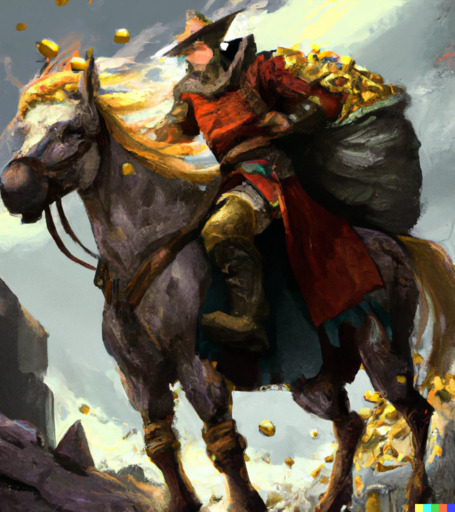
\includegraphics[width=\columnwidth]{equipment/tools goods and mounts}

        The world of Rise has a wide range of minor items like backpacks, blankets, and ten-foot poles.
        In general, the cost of those items is so insignificant from the perspective of an adventuring party that it's not worth the effort to track their cost in detail.
        A subset of particularly expensive items is included in \tref{Permanent Tools, Goods, and Mounts}.

        \subsection{Standard Adventuring Kit}\label{Standard Adventuring Kit}
          % Technically 15.2 gp and 50.5 pounds
          A standard adventuring kit is a rank 0 item (1 gp), weighs 50 pounds, and contains the following items:
          \begin{raggeditemize}
            \item Backpack
            \item Bedroll
            \item Flint and steel
            \item Rations, trail (8 days)
            \item Rope, hempen (60 ft.)
            \item Sack (empty)
            \item Tent
            \item Torch
            \item Waterskin
          \end{raggeditemize}
      \end{longtablepreface}

      \input{generated/permanent_tools_table.tex}
  \end{longcolumn}

  \input{generated/permanent_tools.tex}

  % Magic consumables are a loosely limited slot, but being consumable is a big downside.
  % They have the same power level as spells.
  \begin{longcolumn}
    \section{Consumables}\label{Consumables}

      \subsection{Potions}
        A potion is a magical liquid that is typically contained in a Fine vial.
        Drinking a potion, or administering a potion to an unconscious creature, requires a standard action.
        Potions cannot be safely mixed together without diluting their magic, so you cannot consume two potions with the same action.

        \input{generated/consumable_tools_table.tex}
  \end{longcolumn}

  \input{generated/consumable_tools.tex}

% Magic weapons are a highly limited slot.
% They have the same power level as self-attune spells.
\begin{longcolumn}
    \section{Magic Weapons}\label{Magic Weapons}
    \begin{longtablepreface}

      Magic weapons improve a character's combat abilities.
      They must be wielded to gain their effects.

      \parhead{Ranged Weapons and Ammunition} Any magical properties of a \weapontag{Projectile} weapon also apply to all ammunition fired from that weapon.

      \parhead{Craft Skills} The craft skills used to create and repair items are listed in parentheses before the item's description.
      All magic weapons simply use the same materials as the original, nonmagical weapon.

      \parhead{Property Limits} Normally, a weapon can only have one magic item property.
      \weapontag{Heavy} items can have two magic item properties instead of one.
    \end{longtablepreface}

    \input{generated/magic_weapons_table.tex}

\end{longcolumn}

\input{generated/magic_weapons.tex}

% Magic armor is a highly limited slot.
% They have the same power level as self-attune spells.
\begin{longcolumn}
  \section{Magic Armor}\label{Magic Armor}
    \begin{longtablepreface}
      Magic body armor must be worn to gain its effects, while magic shields must be wielded.
      You cannot imbue magic body armor effects on ordinary clothing, even if that clothing is worn on the body instead of armor.

      \parhead{Property Limits} A suit of body armor can only have one magic item property.
      A shield can also have one magic item property.
    \end{longtablepreface}

    \input{generated/magic_armor_table.tex}

\end{longcolumn}

\input{generated/magic_armor.tex}

% Magic apparel is a loosely limited slot.
% They are one rank behind self-attune spells.
\begin{longcolumn}
  \section{Magic Apparel}
    \begin{longtablepreface}
      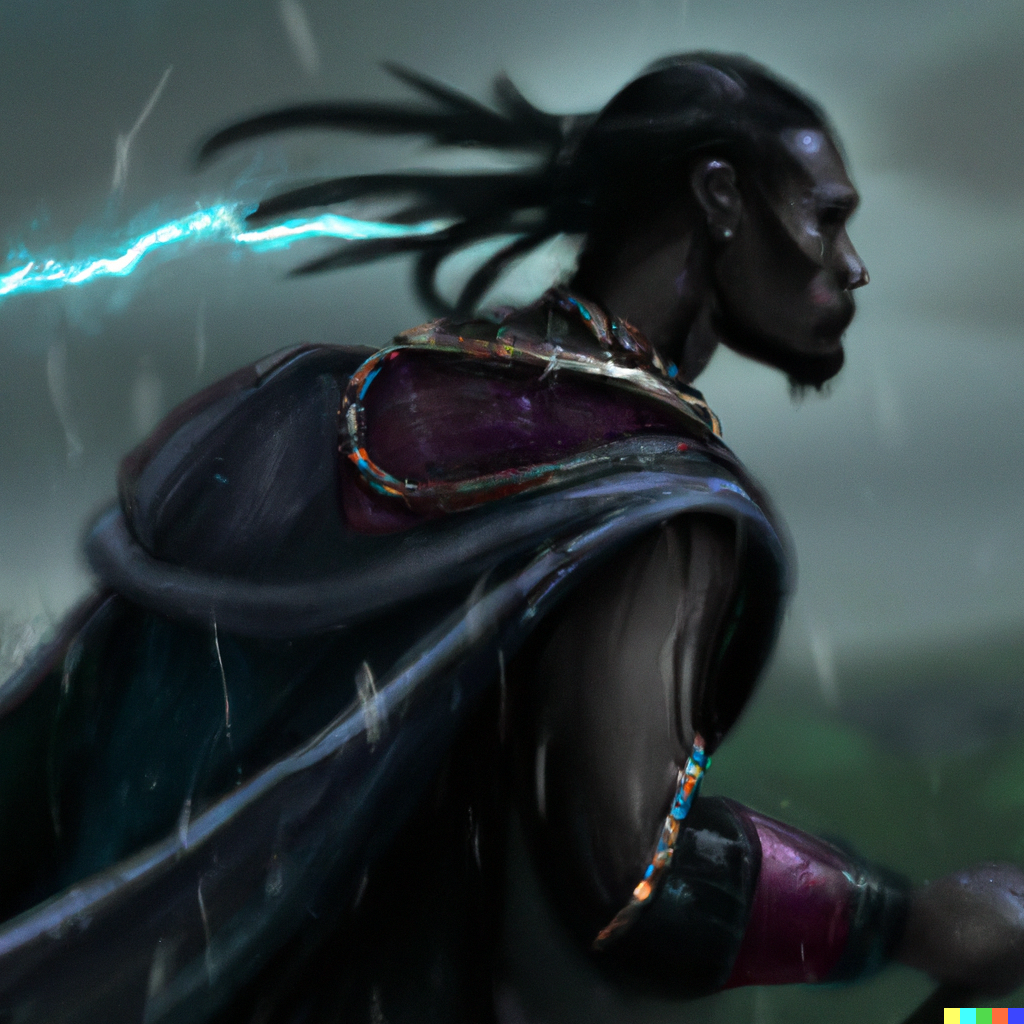
\includegraphics[width=\columnwidth]{equipment/magic apparel}
      Magic apparel items must be worn to gain their effects.

      \subsection{Body Slots}\label{Body Slots}
        The main limiting factor on how many items you can have equipped is your attunement points, not the physical location of your items on your body.
        However, there are limits to how many items you can wear of the same type, as described below.
        For item types not listed here, use reasonable judgment about what would be plausible.
        \begin{raggeditemize}
          \item Amulet: Up to 2
          \item Belt: Up to 2
          \item Boots: Up to 1
          \item Circlet: Up to 2
          \item Cloak: Up to 2
          \item Gauntlets: Up to 1 (separate from gloves)
          \item Gloves: Up to 1 (separate from gauntlets)
          \item Rings: Up to 5 per hand
          \item Tattoo: Any number, but only 1 per specific tattoo location
        \end{raggeditemize}

      \parhead{Property Limits} An apparel item can only have one magic item property.
    \end{longtablepreface}

    
\begin{longtablewrapper}
\begin{longtable}{p{15em} p{3em} p{6em} p{25em} p{3em}}

\lcaption{Apparel Items} \\
\tb{Name} & \tb{Level} & \tb{Typical Price} & \tb{Description} & \tb{Page} \tableheaderrule
Bracers of Archery & \nth{1} & 50 gp & Grants bow proficiency & \pageref{item:Bracers of Archery} \\
Belt of Healing & \nth{2} & 125 gp & Grants healing & \pageref{item:Belt of Healing} \\
Boots of the Winterlands & \nth{2} & 125 gp & Eases travel in cold areas & \pageref{item:Boots of the Winterlands} \\
Bracers of Armor & \nth{2} & 125 gp & Grants invisible armor & \pageref{item:Bracers of Armor} \\
Gauntlets of Improvisation & \nth{2} & 125 gp & Grants \plus1d damage with improvised weapons & \pageref{item:Gauntlets of Improvisation} \\
Ring of Elemental Endurance & \nth{2} & 125 gp & Grants tolerance of temperature extremes & \pageref{item:Ring of Elemental Endurance} \\
Shield of Bashing & \nth{2} & 125 gp & Grants \plus2 power & \pageref{item:Shield of Bashing} \\
Torchlight Gloves & \nth{2} & 125 gp & Sheds light as a torch & \pageref{item:Torchlight Gloves} \\
Ocular Circlet & \nth{3} & 250 gp & Can allow you to see at a distance & \pageref{item:Ocular Circlet} \\
Ring of Nourishment & \nth{3} & 250 gp & Provides food and water & \pageref{item:Ring of Nourishment} \\
Boots of Earth's Embrace & \nth{4} & 500 gp & Grants immunity to forced movement & \pageref{item:Boots of Earth's Embrace} \\
Boots of Elvenkind & \nth{4} & 500 gp & Grants \plus2 Stealth & \pageref{item:Boots of Elvenkind} \\
Circlet of Persuasion & \nth{4} & 500 gp & Grants \plus2 Persuasion & \pageref{item:Circlet of Persuasion} \\
Gauntlet of the Ram & \nth{4} & 500 gp & Knocks back foe when used to strike & \pageref{item:Gauntlet of the Ram} \\
Mask of Water Breathing & \nth{4} & 500 gp & Allows breathing water like air & \pageref{item:Mask of Water Breathing} \\
Throwing Gloves & \nth{4} & 500 gp & Allows throwing any item accurately & \pageref{item:Throwing Gloves} \\
Acid Coated & \nth{5} & 800 gp & Deals acid damage to anything it touches & \pageref{item:Acid Coated} \\
Amulet of Translocation & \nth{5} & 800 gp & Grants ability to teleport up to 30 feet & \pageref{item:Amulet of Translocation} \\
Circlet of Blasting & \nth{5} & 800 gp & Can blast foe with fire & \pageref{item:Circlet of Blasting} \\
Hidden Armor & \nth{5} & 800 gp & Can look like normal clothing & \pageref{item:Hidden Armor} \\
Protective Armor & \nth{5} & 800 gp & Grants \plus1 Armor defense & \pageref{item:Protective Armor} \\
Protective Shield & \nth{5} & 800 gp & Grants \plus1 Armor defense & \pageref{item:Protective Shield} \\
Shield of Arrow Catching & \nth{5} & 800 gp & Redirects small nearby projectiles to hit you & \pageref{item:Shield of Arrow Catching} \\
Shield of Arrow Deflection & \nth{5} & 800 gp & Blocks small projectiles & \pageref{item:Shield of Arrow Deflection} \\
Translocation & \nth{5} & 800 gp & Grants ability to teleport up to 30 feet & \pageref{item:Translocation} \\
Agile & \nth{6} & 1,200 gp & Grants \plus2 Reflex defense & \pageref{item:Agile} \\
Amulet of Health & \nth{6} & 1,200 gp & Grants 2 additional hit points & \pageref{item:Amulet of Health} \\
Amulet of Nondetection & \nth{6} & 1,200 gp & Grants \plus4 to defenses against detection & \pageref{item:Amulet of Nondetection} \\
Boots of Speed & \nth{6} & 1,200 gp & Increases speed by ten feet & \pageref{item:Boots of Speed} \\
Featherlight Armor & \nth{6} & 1,200 gp & Reduces encumbrance by 1 & \pageref{item:Featherlight Armor} \\
Fortified & \nth{6} & 1,200 gp & Grants \plus2 Fortitude defense & \pageref{item:Fortified} \\
Quilled Cloak & \nth{6} & 1,200 gp & Deals damage to creatures that grapple you & \pageref{item:Quilled Cloak} \\
Willguard & \nth{6} & 1,200 gp & Grants \plus2 Mental defense & \pageref{item:Willguard} \\
Anchoring & \nth{7} & 1,800 gp & Protects you from most forced movement attacks & \pageref{item:Anchoring} \\
Armor of Fortification & \nth{7} & 1,800 gp & Reduces critical hits from strikes & \pageref{item:Armor of Fortification} \\
Boots of Water Walking & \nth{7} & 1,800 gp & Allows walking on liquids & \pageref{item:Boots of Water Walking} \\
Boots of the Skydancer & \nth{7} & 1,800 gp & Can walk on air & \pageref{item:Boots of the Skydancer} \\
Bracers of Archery, Greater & \nth{7} & 1,800 gp & Grants bow proficiency, \plus1 ranged accuracy & \pageref{item:Bracers of Archery, Greater} \\
Bracers of Repulsion & \nth{7} & 1,800 gp & Can knock nearby creatures back & \pageref{item:Bracers of Repulsion} \\
Crown of Lightning & \nth{7} & 1,800 gp & Continuously damages nearby enemies & \pageref{item:Crown of Lightning} \\
Gauntlet of the Ram, Greater & \nth{7} & 1,800 gp & Knocks back foe farther when use to strike & \pageref{item:Gauntlet of the Ram, Greater} \\
Gauntlets of Improvisation, Greater & \nth{7} & 1,800 gp & Grants \plus2d damage with improvised weapons & \pageref{item:Gauntlets of Improvisation, Greater} \\
Gloves of Spell Investment & \nth{7} & 1,800 gp & Can invest a spell to cast later & \pageref{item:Gloves of Spell Investment} \\
Hexward Amulet & \nth{7} & 1,800 gp & Grants \plus1 defenses against targeted magical attacks & \pageref{item:Hexward Amulet} \\
Lifekeeping Belt & \nth{7} & 1,800 gp & Grants \plus1 bonus to \glossterm{vital rolls} & \pageref{item:Lifekeeping Belt} \\
Ring of Sustenance & \nth{7} & 1,800 gp & Provides food, water, and rest & \pageref{item:Ring of Sustenance} \\
Amulet of Mighty Fists & \nth{8} & 2,750 gp & Grants \plus2 power with natural and unarmed attacks & \pageref{item:Amulet of Mighty Fists} \\
Armor of Energy Resistance & \nth{8} & 2,750 gp & Reduces energy damage & \pageref{item:Armor of Energy Resistance} \\
Armor of Invulnerability & \nth{8} & 2,750 gp & Reduces physical damage & \pageref{item:Armor of Invulnerability} \\
Assassin's Cloak & \nth{8} & 2,750 gp & Grants invisibility while inactive & \pageref{item:Assassin's Cloak} \\
Avian Cloak & \nth{8} & 2,750 gp & Grants a glide speed & \pageref{item:Avian Cloak} \\
Belt of Healing, Greater & \nth{8} & 2,750 gp & Grants more healing & \pageref{item:Belt of Healing, Greater} \\
Boots of Gravitation & \nth{8} & 2,750 gp & Redirects personal gravity & \pageref{item:Boots of Gravitation} \\
Cloak of Mist & \nth{8} & 2,750 gp & Fills nearby area with fog & \pageref{item:Cloak of Mist} \\
Ring of Protection & \nth{8} & 2,750 gp & Grants \plus1 to Armor and Reflex defenses & \pageref{item:Ring of Protection} \\
Shield of Boulder Catching & \nth{8} & 2,750 gp & Redirects large nearby projectiles to hit you & \pageref{item:Shield of Boulder Catching} \\
Shield of Boulder Deflection & \nth{8} & 2,750 gp & Can block large projectiles & \pageref{item:Shield of Boulder Deflection} \\
Crown of Flame & \nth{9} & 4,000 gp & Grants nearby allies immunity to fire damage & \pageref{item:Crown of Flame} \\
Greatreach Bracers & \nth{9} & 4,000 gp & Increases reach by five feet & \pageref{item:Greatreach Bracers} \\
Hidden Armor, Greater & \nth{9} & 4,000 gp & Can look and sound like normal clothing & \pageref{item:Hidden Armor, Greater} \\
Mask of Air & \nth{9} & 4,000 gp & Allows breathing in any environment & \pageref{item:Mask of Air} \\
Ocular Circlet, Greater & \nth{9} & 4,000 gp & Can allow you to see at a greater distance & \pageref{item:Ocular Circlet, Greater} \\
Ring of Angel's Grace & \nth{9} & 4,000 gp & Grants \plus2 Mental and slows falls & \pageref{item:Ring of Angel's Grace} \\
Boots of Speed, Greater & \nth{10} & 6,500 gp & Increases speed by twenty feet & \pageref{item:Boots of Speed, Greater} \\
Circlet of Blasting, Greater & \nth{10} & 6,500 gp & Can blast foe with intense fire & \pageref{item:Circlet of Blasting, Greater} \\
Crater Boots & \nth{10} & 6,500 gp & Deals your falling damage to enemies & \pageref{item:Crater Boots} \\
Titan Gauntlets & \nth{10} & 6,500 gp & Grants \plus2 \glossterm{mundane} power & \pageref{item:Titan Gauntlets} \\
Winged Boots & \nth{10} & 6,500 gp & Grants limited flight & \pageref{item:Winged Boots} \\
Amulet of Translocation, Greater & \nth{11} & 10,000 gp & Grants ability to teleport up to 100 feet & \pageref{item:Amulet of Translocation, Greater} \\
Crown of Thunder & \nth{11} & 10,000 gp & Continously deafens nearby enemies & \pageref{item:Crown of Thunder} \\
Shield of Arrow Catching, Greater & \nth{11} & 10,000 gp & Selectively redirects small nearby projectiles to hit you & \pageref{item:Shield of Arrow Catching, Greater} \\
Shield of Bashing, Greater & \nth{11} & 10,000 gp & Grants \plus4 power & \pageref{item:Shield of Bashing, Greater} \\
Translocation, Greater & \nth{11} & 10,000 gp & Grants ability to teleport up to 100 feet & \pageref{item:Translocation, Greater} \\
Amulet of the Planes & \nth{12} & 16,000 gp & Aids travel with \ritual{plane shift} & \pageref{item:Amulet of the Planes} \\
Armor of Fortification, Mystic & \nth{12} & 16,000 gp & Reduces critical hits from all attacks & \pageref{item:Armor of Fortification, Mystic} \\
Boots of Freedom & \nth{12} & 16,000 gp & Grants immunity to almost all mobility restrictions & \pageref{item:Boots of Freedom} \\
Featherlight Armor, Greater & \nth{12} & 16,000 gp & Reduces encumbrance by 2 & \pageref{item:Featherlight Armor, Greater} \\
Greater Quilled Cloak & \nth{12} & 16,000 gp & Deals more damage to creatures that grapple you & \pageref{item:Greater Quilled Cloak} \\
Ring of Energy Resistance & \nth{12} & 16,000 gp & Reduces energy damage & \pageref{item:Ring of Energy Resistance} \\
Seven League Boots & \nth{12} & 16,000 gp & Teleport seven leages with a step & \pageref{item:Seven League Boots} \\
Shield of Mystic Reflection & \nth{12} & 16,000 gp & React to reflect magical attacks & \pageref{item:Shield of Mystic Reflection} \\
Anchoring, Greater & \nth{13} & 25,000 gp & Protects you from all forced movement and teleportation attacks & \pageref{item:Anchoring, Greater} \\
Assassin's Cloak, Greater & \nth{13} & 25,000 gp & Grants longer invisibility while inactive & \pageref{item:Assassin's Cloak, Greater} \\
Boots of the Skydancer, Greater & \nth{13} & 25,000 gp & description & \pageref{item:Boots of the Skydancer, Greater} \\
Crown of Frost & \nth{13} & 25,000 gp & Continuously damages nearby enemies & \pageref{item:Crown of Frost} \\
Gloves of Spell Investment, Greater & \nth{13} & 25,000 gp & Can invest two spells to cast later & \pageref{item:Gloves of Spell Investment, Greater} \\
Hexproof Amulet, Greater & \nth{13} & 25,000 gp & Grants \plus2 defenses against targeted magical attacks & \pageref{item:Hexproof Amulet, Greater} \\
Lifekeeping Belt, Greater & \nth{13} & 25,000 gp & Grants \plus2 bonus to \glossterm{vital rolls} & \pageref{item:Lifekeeping Belt, Greater} \\
Vanishing Cloak & \nth{13} & 25,000 gp & Can teleport a short distance and grant invisibility & \pageref{item:Vanishing Cloak} \\
Amulet of Nondetection, Greater & \nth{14} & 37,000 gp & Grants \plus8 to defenses against detection & \pageref{item:Amulet of Nondetection, Greater} \\
Armor of Energy Resistance, Greater & \nth{14} & 37,000 gp & Significantly reduces energy damage & \pageref{item:Armor of Energy Resistance, Greater} \\
Armor of Invulnerability & \nth{14} & 37,000 gp & Significantly reduces physical damage & \pageref{item:Armor of Invulnerability} \\
Belt of Healing, Supreme & \nth{14} & 37,000 gp & Grants more healing & \pageref{item:Belt of Healing, Supreme} \\
Boots of Speed, Supreme & \nth{14} & 37,000 gp & Increases speed by thirty feet & \pageref{item:Boots of Speed, Supreme} \\
Protective Armor, Greater & \nth{14} & 37,000 gp & Grants \plus2 Armor defense & \pageref{item:Protective Armor, Greater} \\
Protective Shield, Greater & \nth{14} & 37,000 gp & Grants \plus2 Armor defense & \pageref{item:Protective Shield, Greater} \\
Shield of Arrow Deflection, Greater & \nth{14} & 37,000 gp & Blocks small projectiles & \pageref{item:Shield of Arrow Deflection, Greater} \\
Agile, Greater & \nth{15} & 55,000 gp & Grants \plus4 Reflex defense & \pageref{item:Agile, Greater} \\
Amulet of Health, Greater & \nth{15} & 55,000 gp & Grants 4 additional hit points & \pageref{item:Amulet of Health, Greater} \\
Armor of Fortification, Greater & \nth{15} & 55,000 gp & Drastically reduces critical hits from strikes & \pageref{item:Armor of Fortification, Greater} \\
Bracers of Repulsion, Greater & \nth{15} & 55,000 gp & Can knock many nearby creatures back & \pageref{item:Bracers of Repulsion, Greater} \\
Fortified, Greater & \nth{15} & 55,000 gp & Grants \plus4 Fortitude defense & \pageref{item:Fortified, Greater} \\
Ring of Regeneration & \nth{15} & 55,000 gp & Automatically removes vital wounds & \pageref{item:Ring of Regeneration} \\
Willguard, Greater & \nth{15} & 55,000 gp & Grants \plus4 Mental defense & \pageref{item:Willguard, Greater} \\
Amulet of Mighty Fists, Greater & \nth{16} & 85,000 gp & Grants \plus4 power with natural and unarmed attacks & \pageref{item:Amulet of Mighty Fists, Greater} \\
Astral Boots & \nth{16} & 85,000 gp & Allows teleporting instead of moving & \pageref{item:Astral Boots} \\
Circlet of Blasting, Supreme & \nth{16} & 85,000 gp & Can blast foe with supremely intense fire & \pageref{item:Circlet of Blasting, Supreme} \\
Cloak of Mist, Greater & \nth{16} & 85,000 gp & Fills nearby area with thick fog & \pageref{item:Cloak of Mist, Greater} \\
Ring of Protection, Greater & \nth{16} & 85,000 gp & Grants \plus2 to Armor and Reflex defenses & \pageref{item:Ring of Protection, Greater} \\
Amulet of Translocation, Supreme & \nth{17} & 125,000 gp & Grants ability to teleport up to 300 feet & \pageref{item:Amulet of Translocation, Supreme} \\
Greatreach Bracers, Greater & \nth{17} & 125,000 gp & Increases reach by ten feet & \pageref{item:Greatreach Bracers, Greater} \\
Shield of Boulder Deflection, Greater & \nth{17} & 125,000 gp & Blocks large projectiles & \pageref{item:Shield of Boulder Deflection, Greater} \\
Translocation, Supreme & \nth{17} & 125,000 gp & Grants ability to teleport up to 300 feet & \pageref{item:Translocation, Supreme} \\
Featherlight Armor, Supreme & \nth{18} & 190,000 gp & Reduces encumbrance by 2 & \pageref{item:Featherlight Armor, Supreme} \\
Supreme Quilled Cloak & \nth{18} & 190,000 gp & Deals even more damage to creatures that grapple you & \pageref{item:Supreme Quilled Cloak} \\
Hexproof Amulet, Supreme & \nth{19} & 280,000 gp & Grants \plus3 defenses against targeted magical attacks & \pageref{item:Hexproof Amulet, Supreme} \\
Lifekeeping Belt, Supreme & \nth{19} & 280,000 gp & Grants \plus3 bonus to \glossterm{vital rolls} & \pageref{item:Lifekeeping Belt, Supreme} \\
Titan Gauntlets, Greater & \nth{19} & 280,000 gp & Grants \plus4 \glossterm{mundane} power & \pageref{item:Titan Gauntlets, Greater} \\
Armor of Energy Resistance, Supreme & \nth{20} & 400,000 gp & Drastically reduces energy damage & \pageref{item:Armor of Energy Resistance, Supreme} \\
Armor of Invulnerability, Greater & \nth{20} & 400,000 gp & Drastically reduces physical damage & \pageref{item:Armor of Invulnerability, Greater} \\
Shield of Bashing, Supreme & \nth{20} & 400,000 gp & Grants \plus6 power & \pageref{item:Shield of Bashing, Supreme} \\

\end{longtable}
\end{longtablewrapper}


\end{longcolumn}

\lowercase{\hypertarget{item:Amulet of Mighty Fists}{}}\label{item:Amulet of Mighty Fists}
\hypertarget{item:Amulet of Mighty Fists}{\subsubsection{Amulet of Mighty Fists\hfill\nth{6}}}
You gain a \plus1d bonus to \glossterm{strike damage} with \glossterm{unarmed attacks} and natural weapons.
\parhead*{Tags} \glossterm{Enhancement}
\parhead*{Materials} Jewelry
\lowercase{\hypertarget{item:Amulet of Mighty Fists, Greater}{}}\label{item:Amulet of Mighty Fists, Greater}
\hypertarget{item:Amulet of Mighty Fists, Greater}{\subsubsection{Amulet of Mighty Fists, Greater\hfill\nth{14}}}
You gain a \plus2d bonus to \glossterm{strike damage} with \glossterm{unarmed attacks} and natural weapons.
\parhead*{Tags} \glossterm{Enhancement}
\parhead*{Materials} Jewelry
\lowercase{\hypertarget{item:Armor of Energy Resistance}{}}\label{item:Armor of Energy Resistance}
\hypertarget{item:Armor of Energy Resistance}{\subsubsection{Armor of Energy Resistance\hfill\nth{4}}}
You have \glossterm{damage reduction} equal to the item's \glossterm{power} against \glossterm{energy damage}.
Whenever you resist energy with this item, it sheds light as a torch until the end of the next round.
The color of the light depends on the energy damage resisted: blue for cold, yellow for electricity, red for fire, and brown for sonic.
\parhead*{Tags} \glossterm{Shielding}
\parhead*{Materials} Bone, metal
\lowercase{\hypertarget{item:Armor of Energy Resistance, Greater}{}}\label{item:Armor of Energy Resistance, Greater}
\hypertarget{item:Armor of Energy Resistance, Greater}{\subsubsection{Armor of Energy Resistance, Greater\hfill\nth{12}}}
This item functions like the \mitem{armor of energy resistance} item, except that the damage reduction is equal to twice the item's \glossterm{power}.
\parhead*{Tags} \glossterm{Shielding}
\parhead*{Materials} Bone, metal
\lowercase{\hypertarget{item:Armor of Fortification}{}}\label{item:Armor of Fortification}
\hypertarget{item:Armor of Fortification}{\subsubsection{Armor of Fortification\hfill\nth{7}}}
You gain a \plus5 bonus to defenses when determining whether a \glossterm{strike} gets a \glossterm{critical hit} against you instead of a normal hit.
\parhead*{Tags} \glossterm{Imbuement}
\parhead*{Materials} Bone, metal
\lowercase{\hypertarget{item:Armor of Fortification, Greater}{}}\label{item:Armor of Fortification, Greater}
\hypertarget{item:Armor of Fortification, Greater}{\subsubsection{Armor of Fortification, Greater\hfill\nth{15}}}
This item functions like the \mitem{armor of fortification} item, except that the bonus increases to \plus10.
\parhead*{Tags} \glossterm{Imbuement}
\parhead*{Materials} Bone, metal
\lowercase{\hypertarget{item:Armor of Fortification, Mystic}{}}\label{item:Armor of Fortification, Mystic}
\hypertarget{item:Armor of Fortification, Mystic}{\subsubsection{Armor of Fortification, Mystic\hfill\nth{12}}}
This item functions like the \mitem{armor of fortification} item, except that it applies against all attacks instead of only against; \glossterm{strikes}.
\parhead*{Tags} \glossterm{Imbuement}
\parhead*{Materials} Bone, metal
\lowercase{\hypertarget{item:Armor of Invulnerability}{}}\label{item:Armor of Invulnerability}
\hypertarget{item:Armor of Invulnerability}{\subsubsection{Armor of Invulnerability\hfill\nth{8}}}
You have \glossterm{damage reduction} equal to this item's \glossterm{power} against damage from \glossterm{physical attacks}.
\parhead*{Tags} \glossterm{Shielding}
\parhead*{Materials} Bone, metal
\lowercase{\hypertarget{item:Armor of Invulnerability, Greater}{}}\label{item:Armor of Invulnerability, Greater}
\hypertarget{item:Armor of Invulnerability, Greater}{\subsubsection{Armor of Invulnerability, Greater\hfill\nth{16}}}
This item functions like the \mitem{armor of invulnerability} item, except that the damage reduction is equal to twice the item's \glossterm{power}.
You have \glossterm{damage reduction} equal to the item's \glossterm{power} against damage from \glossterm{physical attacks}.
\parhead*{Tags} \glossterm{Shielding}
\parhead*{Materials} Bone, metal
\lowercase{\hypertarget{item:Armor of Magic Resistance}{}}\label{item:Armor of Magic Resistance}
\hypertarget{item:Armor of Magic Resistance}{\subsubsection{Armor of Magic Resistance\hfill\nth{14}}}
You have \glossterm{magic resistance} equal to 5 + the item's \glossterm{power}.
\parhead*{Tags} \glossterm{Shielding}
\parhead*{Materials} Bone, metal
\lowercase{\hypertarget{item:Assassin's Cloak}{}}\label{item:Assassin's Cloak}
\hypertarget{item:Assassin's Cloak}{\subsubsection{Assassin's Cloak\hfill\nth{7}}}
At the end of each round, if you took no actions that round, you become \glossterm{invisible} until the end of the next round.
\parhead*{Tags} \glossterm{Glamer}
\parhead*{Materials} Textiles
\lowercase{\hypertarget{item:Assassin's Cloak, Greater}{}}\label{item:Assassin's Cloak, Greater}
\hypertarget{item:Assassin's Cloak, Greater}{\subsubsection{Assassin's Cloak, Greater\hfill\nth{17}}}
At the end of each round, if you did not attack a creature that round, you become \glossterm{invisible} until the end of the next round.
\parhead*{Tags} \glossterm{Glamer}
\parhead*{Materials} Textiles
\lowercase{\hypertarget{item:Astral Boots}{}}\label{item:Astral Boots}
\hypertarget{item:Astral Boots}{\subsubsection{Astral Boots\hfill\nth{16}}}
Whenever you move, you can teleport the same distance instead.
This does not change the total distance you can move, but you can teleport in any direction, even vertically.
You cannot teleport to locations you do not have \glossterm{line of sight} and \glossterm{line of effect} to.
\parhead*{Tags} \glossterm{Teleportation}
\parhead*{Materials} Bone, leather, metal
\lowercase{\hypertarget{item:Belt of Healing}{}}\label{item:Belt of Healing}
\hypertarget{item:Belt of Healing}{\subsubsection{Belt of Healing\hfill\nth{1}}}
When you use the \textit{recover} action, you heal \plus1d hit points.
\parhead*{Tags} \glossterm{Life}
\parhead*{Materials} Leather, textiles
\lowercase{\hypertarget{item:Belt of Healing, Greater}{}}\label{item:Belt of Healing, Greater}
\hypertarget{item:Belt of Healing, Greater}{\subsubsection{Belt of Healing, Greater\hfill\nth{8}}}
When you use the \textit{recover} action, you heal \plus2d hit points.
\parhead*{Tags} \glossterm{Life}
\parhead*{Materials} Leather, textiles
\lowercase{\hypertarget{item:Belt of Heroic Recovery}{}}\label{item:Belt of Heroic Recovery}
\hypertarget{item:Belt of Heroic Recovery}{\subsubsection{Belt of Heroic Recovery\hfill\nth{6}}}
% TODO: timing?
As an \glossterm{immediate action} when you get a \glossterm{critical hit}, you can take the \textit{recover} action.
\parhead*{Tags} \glossterm{Life}
\parhead*{Materials} Leather, textiles
\lowercase{\hypertarget{item:Boots of Earth's Embrace}{}}\label{item:Boots of Earth's Embrace}
\hypertarget{item:Boots of Earth's Embrace}{\subsubsection{Boots of Earth's Embrace\hfill\nth{4}}}
While you are standing on solid ground, you are immune to effects that would force you to move.
This does not protect you from other effects of those attacks, such as damage.
\parhead*{Tags} \glossterm{Earth}, \glossterm{Enhancement}
\parhead*{Materials} Bone, leather, metal
\lowercase{\hypertarget{item:Boots of Freedom}{}}\label{item:Boots of Freedom}
\hypertarget{item:Boots of Freedom}{\subsubsection{Boots of Freedom\hfill\nth{6}}}
You are immune to effects that restrict your mobility.
This removes all penalties you would suffer for acting underwater, except for those relating to using ranged weapons.
This does not prevent you from being \grappled, but you gain a \plus10 bonus to your defense against \glossterm{grapple} attacks.
\parhead*{Tags} \glossterm{Imbuement}
\parhead*{Materials} Bone, leather, metal
\lowercase{\hypertarget{item:Boots of Freedom, Greater}{}}\label{item:Boots of Freedom, Greater}
\hypertarget{item:Boots of Freedom, Greater}{\subsubsection{Boots of Freedom, Greater\hfill\nth{12}}}
These boots function like \mitem{boots of freedom}, except that you are also immune to being \grappled.
\parhead*{Tags} \glossterm{Imbuement}
\parhead*{Materials} Bone, leather, metal
\lowercase{\hypertarget{item:Boots of Gravitation}{}}\label{item:Boots of Gravitation}
\hypertarget{item:Boots of Gravitation}{\subsubsection{Boots of Gravitation\hfill\nth{8}}}
While these boots are within 5 feet of a solid surface, gravity pulls you towards the solid surface closest to your boots rather than in the normal direction.
This can allow you to walk easily on walls or even ceilings.
\parhead*{Tags} \glossterm{Imbuement}
\parhead*{Materials} Bone, leather, metal
\lowercase{\hypertarget{item:Boots of Speed}{}}\label{item:Boots of Speed}
\hypertarget{item:Boots of Speed}{\subsubsection{Boots of Speed\hfill\nth{5}}}
You gain a \plus10 foot bonus to your speed in all your movement modes, up to a maximum of double your normal speed.
\parhead*{Tags} \glossterm{Temporal}
\parhead*{Materials} Bone, leather, metal
\lowercase{\hypertarget{item:Boots of Speed, Greater}{}}\label{item:Boots of Speed, Greater}
\hypertarget{item:Boots of Speed, Greater}{\subsubsection{Boots of Speed, Greater\hfill\nth{13}}}
You gain a \plus30 foot bonus to your speed in all your movement modes, up to a maximum of double your normal speed.
\parhead*{Tags} \glossterm{Temporal}
\parhead*{Materials} Bone, leather, metal
\lowercase{\hypertarget{item:Boots of Water Walking}{}}\label{item:Boots of Water Walking}
\hypertarget{item:Boots of Water Walking}{\subsubsection{Boots of Water Walking\hfill\nth{7}}}
You treat the surface of all liquids as if they were firm ground.
Your feet hover about an inch above the liquid's surface, allowing you to traverse dangerous liquids without harm as long as the surface is calm.
If you are below the surface of the liquid, you rise towards the surface at a rate of 60 feet per round.
Thick liquids, such as mud and lava, may cause you to rise more slowly.
\parhead*{Tags} \glossterm{Imbuement}
\parhead*{Materials} Bone, leather, metal
\lowercase{\hypertarget{item:Boots of the Winterlands}{}}\label{item:Boots of the Winterlands}
\hypertarget{item:Boots of the Winterlands}{\subsubsection{Boots of the Winterlands\hfill\nth{2}}}
You can travel across snow and ice without slipping or suffering movement penalties for the terrain.
% TODO: degree symbol?
In addition, the boots keep you warn, protecting you in environments as cold as \minus50 Fahrenheit.
\parhead*{Tags} \glossterm{Enhancement}
\parhead*{Materials} Bone, leather, metal
\lowercase{\hypertarget{item:Bracers of Archery}{}}\label{item:Bracers of Archery}
\hypertarget{item:Bracers of Archery}{\subsubsection{Bracers of Archery\hfill\nth{1}}}
You are proficient with bows.
\parhead*{Tags} \glossterm{Enhancement}
\parhead*{Materials} Bone, leather, metal, wood
\lowercase{\hypertarget{item:Bracers of Armor}{}}\label{item:Bracers of Armor}
\hypertarget{item:Bracers of Armor}{\subsubsection{Bracers of Armor\hfill\nth{2}}}
You gain a \plus2 bonus to Armor defense.
The protection from these bracers is treated as body armor, and it does not stack with any other body armor you wear.
\parhead*{Tags} \glossterm{Shielding}
\parhead*{Materials} Bone, leather, metal, wood
\lowercase{\hypertarget{item:Bracers of Repulsion}{}}\label{item:Bracers of Repulsion}
\hypertarget{item:Bracers of Repulsion}{\subsubsection{Bracers of Repulsion\hfill\nth{4}}}
Whenever a creature hits you with a melee \glossterm{strike} during the \glossterm{action phase},
you can spend an \glossterm{action point} to use this item as an \glossterm{immediate action}.
If you do, you make a \glossterm{shove} attack against that creature during the \glossterm{delayed action phase}, using this item's power in place of your Strength.
\parhead*{Tags} \glossterm{Telekinesis}
\parhead*{Materials} Bone, leather, metal, wood
\lowercase{\hypertarget{item:Bracers of Repulsion, Greater}{}}\label{item:Bracers of Repulsion, Greater}
\hypertarget{item:Bracers of Repulsion, Greater}{\subsubsection{Bracers of Repulsion, Greater\hfill\nth{11}}}
This item functions like the \mitem{bracers of repulsion} item, except that it does not cost an action point to use.
\parhead*{Tags} \glossterm{Telekinesis}
\parhead*{Materials} Bone, leather, metal, wood
\lowercase{\hypertarget{item:Cloak of Mist}{}}\label{item:Cloak of Mist}
\hypertarget{item:Cloak of Mist}{\subsubsection{Cloak of Mist\hfill\nth{8}}}
Fog constantly fills an \areamed radius emanation from you.
This fog does not fully block sight, but it provides \concealment.
If a 5-foot square of fog takes fire damage equal to half this item's \glossterm{power}, the fog disappears from that area until the end of the next round.
\parhead*{Tags} \glossterm{Fog}, \glossterm{Manifestation}
\parhead*{Materials} Textiles
\lowercase{\hypertarget{item:Cloak of Mist, Greater}{}}\label{item:Cloak of Mist, Greater}
\hypertarget{item:Cloak of Mist, Greater}{\subsubsection{Cloak of Mist, Greater\hfill\nth{16}}}
A thick fog constantly fills an \areamed radius emanation from you.
This fog completely blocks sight beyond 10 feet.
Within that range, it still provides \concealment.
If a 5-foot square of fog takes fire damage equal to this item's \glossterm{power}, the fog disappears from that area until the end of the next round.
\parhead*{Tags} \glossterm{Fog}, \glossterm{Manifestation}
\parhead*{Materials} Textiles
\lowercase{\hypertarget{item:Crown of Flame}{}}\label{item:Crown of Flame}
\hypertarget{item:Crown of Flame}{\subsubsection{Crown of Flame\hfill\nth{5}}}
This crown is continuously on fire.
The flame sheds light as a torch.
You and all allies within an \arealarge radius emanation from you are immune to fire damage.
\parhead*{Tags} \glossterm{Fire}
\parhead*{Materials} Bone, metal
\lowercase{\hypertarget{item:Crown of Frost}{}}\label{item:Crown of Frost}
\hypertarget{item:Crown of Frost}{\subsubsection{Crown of Frost\hfill\nth{11}}}
At the end of each \glossterm{action phase}, you make a Power vs. Fortitude attack against all enemies within an \areamed radius emanation from you.
A hit deals cold \glossterm{standard damage} \minus3d.
Each creature that takes damage in this way is \fatigued until the end of the next round.
\parhead*{Tags} \glossterm{Cold}
\parhead*{Materials} Bone, metal
\lowercase{\hypertarget{item:Crown of Lightning}{}}\label{item:Crown of Lightning}
\hypertarget{item:Crown of Lightning}{\subsubsection{Crown of Lightning\hfill\nth{7}}}
This crown continuously crackles with electricity.
The constant sparks shed light as a torch.
At the end of each \glossterm{action phase}, you make a Power vs. Reflex attack against all enemies within an \areamed radius emanation from you.
A hit deals electricity \glossterm{standard damage} \minus3d.
\parhead*{Tags} \glossterm{Electricity}
\parhead*{Materials} Bone, metal
\lowercase{\hypertarget{item:Crown of Thunder}{}}\label{item:Crown of Thunder}
\hypertarget{item:Crown of Thunder}{\subsubsection{Crown of Thunder\hfill\nth{9}}}
The crown constantly emits a low-pitched rumbling.
To you and your allies, the sound is barely perceptible.
However, all enemies within an \arealarge radius emanation from you hear the sound as a deafening, continuous roll of thunder.
The noise blocks out all other sounds quieter than thunder, causing them to be \deafened while they remain in the area and until the end of the next round after they leave.
\parhead*{Tags} \glossterm{Sonic}
\parhead*{Materials} Bone, metal
\lowercase{\hypertarget{item:Featherlight Armor}{}}\label{item:Featherlight Armor}
\hypertarget{item:Featherlight Armor}{\subsubsection{Featherlight Armor\hfill\nth{4}}}
This armor's \glossterm{encumbrance penalty} is reduced by 2.
\parhead*{Tags} \glossterm{Enhancement}
\parhead*{Materials} Bone, metal
\lowercase{\hypertarget{item:Featherlight Armor, Greater}{}}\label{item:Featherlight Armor, Greater}
\hypertarget{item:Featherlight Armor, Greater}{\subsubsection{Featherlight Armor, Greater\hfill\nth{10}}}
This armor's \glossterm{encumbrance penalty} is reduced by 4.
\parhead*{Tags} \glossterm{Enhancement}
\parhead*{Materials} Bone, metal
\lowercase{\hypertarget{item:Gauntlet of the Ram}{}}\label{item:Gauntlet of the Ram}
\hypertarget{item:Gauntlet of the Ram}{\subsubsection{Gauntlet of the Ram\hfill\nth{2}}}
If you hit on a \glossterm{strike} with this gauntlet during the \glossterm{action phse}, you can attempt to \glossterm{shove} your foe during the \glossterm{delayed action phase}.
Making a strike with this gauntlet is equivalent to an \glossterm{unarmed attack}.
You do not need to move with your foe to push it back the full distance.
\parhead*{Tags} \glossterm{Telekinesis}
\parhead*{Materials} Bone, metal, wood
\lowercase{\hypertarget{item:Gauntlet of the Ram, Greater}{}}\label{item:Gauntlet of the Ram, Greater}
\hypertarget{item:Gauntlet of the Ram, Greater}{\subsubsection{Gauntlet of the Ram, Greater\hfill\nth{7}}}
This item functions like the \mitem{gauntlet of the ram}, except that you gain a bonus to the \glossterm{shove} attack equal to the damage you dealt with the \glossterm{strike}.
\parhead*{Tags} \glossterm{Telekinesis}
\parhead*{Materials} Bone, metal, wood
\lowercase{\hypertarget{item:Gauntlets of Improvisation}{}}\label{item:Gauntlets of Improvisation}
\hypertarget{item:Gauntlets of Improvisation}{\subsubsection{Gauntlets of Improvisation\hfill\nth{2}}}
You gain a \plus1d bonus to damage with \glossterm{improvised weapons}.
\parhead*{Tags} \glossterm{Enhancement}
\parhead*{Materials} Bone, metal, wood
\lowercase{\hypertarget{item:Gauntlets of Improvisation, Greater}{}}\label{item:Gauntlets of Improvisation, Greater}
\hypertarget{item:Gauntlets of Improvisation, Greater}{\subsubsection{Gauntlets of Improvisation, Greater\hfill\nth{7}}}
This item functions like the \mitem{gauntlets of improvisation}, except that the damage bonus is increased to \plus2d.
\parhead*{Tags} \glossterm{Enhancement}
\parhead*{Materials} Bone, metal, wood
\lowercase{\hypertarget{item:Greatreach Bracers}{}}\label{item:Greatreach Bracers}
\hypertarget{item:Greatreach Bracers}{\subsubsection{Greatreach Bracers\hfill\nth{9}}}
Your \glossterm{reach} is increased by 5 feet.
\parhead*{Tags} \glossterm{Imbuement}
\parhead*{Materials} Bone, leather, metal, wood
\lowercase{\hypertarget{item:Greatreach Bracers, Greater}{}}\label{item:Greatreach Bracers, Greater}
\hypertarget{item:Greatreach Bracers, Greater}{\subsubsection{Greatreach Bracers, Greater\hfill\nth{17}}}
Your \glossterm{reach} is increased by 10 feet.
\parhead*{Tags} \glossterm{Imbuement}
\parhead*{Materials} Bone, leather, metal, wood
\lowercase{\hypertarget{item:Hexproof Cloak}{}}\label{item:Hexproof Cloak}
\hypertarget{item:Hexproof Cloak}{\subsubsection{Hexproof Cloak\hfill\nth{18}}}
All \glossterm{magical} abilities that target you directly fail to affect you.
This does not protect you from abilities that affect an area.
\parhead*{Tags} \glossterm{Thaumaturgy}
\parhead*{Materials} Textiles
\lowercase{\hypertarget{item:Hexward Cloak}{}}\label{item:Hexward Cloak}
\hypertarget{item:Hexward Cloak}{\subsubsection{Hexward Cloak\hfill\nth{10}}}
You gain a \plus5 bonus to defenses against \glossterm{magical} abilities that target you directly.
This does not protect you from abilities that affect an area.
\parhead*{Tags} \glossterm{Thaumaturgy}
\parhead*{Materials} Textiles
\lowercase{\hypertarget{item:Hidden Armor}{}}\label{item:Hidden Armor}
\hypertarget{item:Hidden Armor}{\subsubsection{Hidden Armor\hfill\nth{4}}}
As a standard action, you can use this item.
If you do, it appears to change shape and form to assume the shape of a normal set of clothing.
You may choose the design of the clothing.
The item retains all of its properties, including weight and sound, while disguised in this way.
Only its visual appearance is altered.
Alternately, you may return the armor to its original appearance.
\parhead*{Tags} \glossterm{Glamer}
\parhead*{Materials} Bone, metal
\lowercase{\hypertarget{item:Hidden Armor, Greater}{}}\label{item:Hidden Armor, Greater}
\hypertarget{item:Hidden Armor, Greater}{\subsubsection{Hidden Armor, Greater\hfill\nth{9}}}
This item functions like the \mitem{hidden armor} item, except that the item also makes sound appropriate to its disguised form while disguised.
\parhead*{Tags} \glossterm{Alteration}
\parhead*{Materials} Bone, metal
\lowercase{\hypertarget{item:Mask of Air}{}}\label{item:Mask of Air}
\hypertarget{item:Mask of Air}{\subsubsection{Mask of Air\hfill\nth{9}}}
If you breathe through this mask, you breathe in clean, fresh air, regardless of your environment.
This can protect you from inhaled poisons and similar effects.
\parhead*{Tags} \glossterm{Imbuement}
\parhead*{Materials} Textiles
\lowercase{\hypertarget{item:Mask of Water Breathing}{}}\label{item:Mask of Water Breathing}
\hypertarget{item:Mask of Water Breathing}{\subsubsection{Mask of Water Breathing\hfill\nth{4}}}
You can breathe water through this mask as easily as a human breaths air.
This does not grant you the ability to breathe other liquids.
\parhead*{Tags} \glossterm{Imbuement}
\parhead*{Materials} Textiles
\lowercase{\hypertarget{item:Ring of Elemental Endurance}{}}\label{item:Ring of Elemental Endurance}
\hypertarget{item:Ring of Elemental Endurance}{\subsubsection{Ring of Elemental Endurance\hfill\nth{2}}}
You can exist comfortably in conditions between \minus50 and 140 degrees Fahrenheit without any ill effects.
You suffer the normal penalties in temperatures outside of that range.
\parhead*{Tags} \glossterm{Shielding}
\parhead*{Materials} Bone, jewelry, metal, wood
\lowercase{\hypertarget{item:Ring of Energy Resistance}{}}\label{item:Ring of Energy Resistance}
\hypertarget{item:Ring of Energy Resistance}{\subsubsection{Ring of Energy Resistance\hfill\nth{6}}}
You have \glossterm{damage reduction} equal to the ring's \glossterm{power} against \glossterm{energy damage}.
Whenever you resist energy with this ability, the ring sheds light as a torch until the end of the next round.
The color of the light depends on the energy damage resisted: blue for cold, yellow for electricity, red for fire, and brown for sonic.
\parhead*{Tags} \glossterm{Shielding}
\parhead*{Materials} Bone, jewelry, metal, wood
\lowercase{\hypertarget{item:Ring of Energy Resistance, Greater}{}}\label{item:Ring of Energy Resistance, Greater}
\hypertarget{item:Ring of Energy Resistance, Greater}{\subsubsection{Ring of Energy Resistance, Greater\hfill\nth{14}}}
This item functions like the \mitem{ring of energy resistance}, except that the damage reduction is equal to twice the item's \glossterm{power}.
\parhead*{Tags} \glossterm{Shielding}
\parhead*{Materials} Bone, jewelry, metal, wood
\lowercase{\hypertarget{item:Ring of Nourishment}{}}\label{item:Ring of Nourishment}
\hypertarget{item:Ring of Nourishment}{\subsubsection{Ring of Nourishment\hfill\nth{3}}}
You continuously gain nourishment, and no longer need to eat or drink.
This ring must be worn for 24 hours before it begins to work.
\parhead*{Tags} \glossterm{Creation}
\parhead*{Materials} Bone, jewelry, metal, wood
\lowercase{\hypertarget{item:Ring of Protection}{}}\label{item:Ring of Protection}
\hypertarget{item:Ring of Protection}{\subsubsection{Ring of Protection\hfill\nth{8}}}
You gain a \plus1 bonus to Armor defense.
\parhead*{Tags} \glossterm{Shielding}
\parhead*{Materials} Bone, jewelry, metal, wood
\lowercase{\hypertarget{item:Ring of Regeneration}{}}\label{item:Ring of Regeneration}
\hypertarget{item:Ring of Regeneration}{\subsubsection{Ring of Regeneration\hfill\nth{11}}}
At the end of each \glossterm{action phase}, you heal hit points equal to this item's \glossterm{power}.
Only damage taken while wearing the ring can be healed in this way.
\parhead*{Tags} \glossterm{Life}
\parhead*{Materials} Bone, jewelry, metal, wood
\lowercase{\hypertarget{item:Ring of Sustenance}{}}\label{item:Ring of Sustenance}
\hypertarget{item:Ring of Sustenance}{\subsubsection{Ring of Sustenance\hfill\nth{7}}}
You continuously gain nourishment, and no longer need to eat or drink.
In addition, you need only one-quarter your normal amount of sleep (or similar activity, such as elven trance) each day.
The ring must be worn for 24 hours before it begins to work.
\parhead*{Tags} \glossterm{Creation}, \glossterm{Temporal}
\parhead*{Materials} Bone, jewelry, metal, wood
\lowercase{\hypertarget{item:Seven League Boots}{}}\label{item:Seven League Boots}
\hypertarget{item:Seven League Boots}{\subsubsection{Seven League Boots\hfill\nth{12}}}
As a standard action, you can spend an \glossterm{action point} to use this item.
If you do, you teleport exactly 25 miles in a direction you specify.
If this would place you within a solid object or otherwise impossible space, the boots will shunt you up to 1,000 feet in any direction to the closest available space.
If there is no available space within 1,000 feet of your intended destination, the effect fails and you take \glossterm{standard damage} \minus1d.
\parhead*{Tags} \glossterm{Teleportation}
\parhead*{Materials} Bone, leather, metal
\lowercase{\hypertarget{item:Shield of Arrow Catching}{}}\label{item:Shield of Arrow Catching}
\hypertarget{item:Shield of Arrow Catching}{\subsubsection{Shield of Arrow Catching\hfill\nth{5}}}
Whenever a creature within a \areamed radius emanation from you would be attacked by a ranged weapon, the attack is redirected to target you instead.
Resolve the attack as if it had initially targeted you, except that the attack is not affected by cover or concealment.
This item can only affect projectiles and thrown objects that are Small or smaller.
\parhead*{Tags} \glossterm{Telekinesis}
\parhead*{Materials} Bone, metal, wood
\lowercase{\hypertarget{item:Shield of Arrow Catching, Greater}{}}\label{item:Shield of Arrow Catching, Greater}
\hypertarget{item:Shield of Arrow Catching, Greater}{\subsubsection{Shield of Arrow Catching, Greater\hfill\nth{10}}}
This item functions like the \mitem{shield of arrow catching} item, except that it affects a \arealarge radius from you.
In addition, you may choose to exclude creature from this item's effect, allowing projectiles to target nearby foes normally.
\parhead*{Tags} \glossterm{Telekinesis}
\parhead*{Materials} Bone, metal, wood
\lowercase{\hypertarget{item:Shield of Arrow Deflection}{}}\label{item:Shield of Arrow Deflection}
\hypertarget{item:Shield of Arrow Deflection}{\subsubsection{Shield of Arrow Deflection\hfill\nth{2}}}
As an \glossterm{immediate action} when you are attacked by a ranged \glossterm{strike}, you can use this item.
If you do, you gain a \plus5 bonus to Armor defense against the attack.
You must be aware of the attack to deflect it in this way.
This item can only affect projectiles and thrown objects that are Small or smaller.
\parhead*{Tags} \glossterm{Telekinesis}
\parhead*{Materials} Bone, metal, wood
\lowercase{\hypertarget{item:Shield of Arrow Deflection, Greater}{}}\label{item:Shield of Arrow Deflection, Greater}
\hypertarget{item:Shield of Arrow Deflection, Greater}{\subsubsection{Shield of Arrow Deflection, Greater\hfill\nth{12}}}
This item functions like the \mitem{shield of arrow deflection} item, except that the defense bonus increases to \plus10.
\parhead*{Tags} \glossterm{Telekinesis}
\parhead*{Materials} Bone, metal, wood
\lowercase{\hypertarget{item:Shield of Bashing}{}}\label{item:Shield of Bashing}
\hypertarget{item:Shield of Bashing}{\subsubsection{Shield of Bashing\hfill\nth{2}}}
% Should this be strike damage?
You gain a \plus1d bonus to damage with \glossterm{physical attacks} using this shield.
\parhead*{Tags} \glossterm{Enhancement}
\parhead*{Materials} Bone, metal, wood
\lowercase{\hypertarget{item:Shield of Bashing, Greater}{}}\label{item:Shield of Bashing, Greater}
\hypertarget{item:Shield of Bashing, Greater}{\subsubsection{Shield of Bashing, Greater\hfill\nth{11}}}
% Should this be strike damage?
You gain a \plus2d bonus to damage with \glossterm{physical attacks} using this shield.
\parhead*{Tags} \glossterm{Enhancement}
\parhead*{Materials} Bone, metal, wood
\lowercase{\hypertarget{item:Shield of Boulder Catching}{}}\label{item:Shield of Boulder Catching}
\hypertarget{item:Shield of Boulder Catching}{\subsubsection{Shield of Boulder Catching\hfill\nth{8}}}
This item functions like the \mitem{shield of arrow catching} item, except that it can affect projectile and thrown objects of up to Large size.
\parhead*{Tags} \glossterm{Telekinesis}
\parhead*{Materials} Bone, metal, wood
\lowercase{\hypertarget{item:Shield of Boulder Deflection}{}}\label{item:Shield of Boulder Deflection}
\hypertarget{item:Shield of Boulder Deflection}{\subsubsection{Shield of Boulder Deflection\hfill\nth{6}}}
This item functions like the \mitem{shield of arrow deflection} item, except that it can affect projectiles and thrown objects of up to Large size.
\parhead*{Tags} \glossterm{Telekinesis}
\parhead*{Materials} Bone, metal, wood
\lowercase{\hypertarget{item:Shield of Mystic Reflection}{}}\label{item:Shield of Mystic Reflection}
\hypertarget{item:Shield of Mystic Reflection}{\subsubsection{Shield of Mystic Reflection\hfill\nth{12}}}
As an \glossterm{immediate action} when you are targeted by a targeted \glossterm{magical} ability, you can spend an \glossterm{action point} to use this ability.
If you do, the ability targets the creature using the ability instead of you.
Any other targets of the ability are affected normally.
\parhead*{Tags} \glossterm{Thaumaturgy}
\parhead*{Materials} Bone, metal, wood
\lowercase{\hypertarget{item:Throwing Gloves}{}}\label{item:Throwing Gloves}
\hypertarget{item:Throwing Gloves}{\subsubsection{Throwing Gloves\hfill\nth{4}}}
% TODO: reference basic "not designed to be thrown" mechanics?
You can throw any item as if it was designed to be thrown.
This does not improve your ability to throw items designed to be thrown, such as darts.
\parhead*{Tags} \glossterm{Enhancement}
\parhead*{Materials} Leather
\lowercase{\hypertarget{item:Torchlight Gloves}{}}\label{item:Torchlight Gloves}
\hypertarget{item:Torchlight Gloves}{\subsubsection{Torchlight Gloves\hfill\nth{2}}}
These gloves shed light as a torch.
As a \glossterm{standard action}, you may choose to suppress or resume the light from either or both gloves.
\parhead*{Tags} \glossterm{Figment}, \glossterm{Light}
\parhead*{Materials} Leather
\lowercase{\hypertarget{item:Vanishing Cloak}{}}\label{item:Vanishing Cloak}
\hypertarget{item:Vanishing Cloak}{\subsubsection{Vanishing Cloak\hfill\nth{8}}}
As a standard action, you can spend an \glossterm{action point} to use this item.
If you do, you teleport to an unoccupied location within \rngmed range of your original location.
In addition, you become \glossterm{invisible} unitl the end of the next round.
If your intended destination is invalid, or if your teleportation otherwise fails, you still become invisible.
\parhead*{Tags} \glossterm{Glamer}, \glossterm{Teleportation}
\parhead*{Materials} Textiles
\lowercase{\hypertarget{item:Winged Boots}{}}\label{item:Winged Boots}
\hypertarget{item:Winged Boots}{\subsubsection{Winged Boots\hfill\nth{10}}}
You gain a \glossterm{fly speed} equal to your land speed.
However, the boots are not strong enough to keep you aloft indefinitely.
At the end of each round, if you are not standing on solid ground, the magic of the boots fails and you fall normally.
The boots begin working again at the end of the next round, even if you have not yet hit the ground.
\parhead*{Tags} \glossterm{Imbuement}
\parhead*{Materials} Bone, leather, metal

  % Magic implements are a highly limited slot.
  % They have the same power level as self-attune spells.
  % This has a lot of text, so we need two columns
\newpage
\sectiongraphic*{Magic Implements}{width=\columnwidth}{equipment/magic implements}

  Like magic weapons, magic implements must be wielded to gain their effects.
  However, while weapons are used to deal damage to enemies, implements are used to grant or enhance magical abilities.

  There are three types of implements: staffs, rods, and wands.
  Staffs improve your existing magical abilities.
  Rods grant new magical abilities, even to those who cannot cast spells.
  Wands grant spellcasters the knowledge of specific spells.

  Staffs are long and thin, with even short staffs measuring no less than four feet long.
  Rods are about three feet long, but sturdily constructed.
  Wands are only about a foot long and very thin.

  \parhead{Somatic Components} While wielding an implement, you may gesture with it to perform \glossterm{somatic components}.
  This means you do not need a separate \glossterm{free hand} to perform those components.

  \parhead{Staff Types}
  There are two types of staffs that you can find.
  A short staff only requires one hand, but it is not suitable as a weapon.
  A long staff functions like a quarterstaff weapon.
  It can have two magic properties instead of one, and you can freely mix weapon properties and implement properties.
  However, it must be held in two hands to grant its benefits.

  \begin{longcolumn}
    
\begin{longtabuwrapper}
\begin{longtabu}{l l X l}
\lcaption{Implement Items} \\
\tb{Name} & \tb{Level} & \tb{Description} & \tb{Page} \\
\bottomrule
Wand of Spellpower & \nth{4} & Grants \plus1 power with a single spell & \pageref{item:Wand of Spellpower} \\
Staff of Transit & \nth{5} & Doubles your teleportation distance & \pageref{item:Staff of Transit} \\
Spellfeeding Staff & \nth{6} & Heals you when casting spells & \pageref{item:Spellfeeding Staff} \\
Staff of Spellpower & \nth{8} & Grants \plus1 power with spells & \pageref{item:Staff of Spellpower} \\
Staff of Sympathetic Shielding & \nth{8} & Shields you when shielding others & \pageref{item:Staff of Sympathetic Shielding} \\
Wand of Precision & \nth{8} & Grants \plus1 accuracy with a single spell & \pageref{item:Wand of Precision} \\
Staff of Precision & \nth{10} & Grants \plus1 accuracy with spells & \pageref{item:Staff of Precision} \\
Wand of Spellpower, Greater & \nth{10} & Grants \plus2 power with a single spell & \pageref{item:Wand of Spellpower, Greater} \\
Spellfeeding Staff, Greater & \nth{14} & Greatly heals you when casting spells & \pageref{item:Spellfeeding Staff, Greater} \\
Staff of Spellpower, Greater & \nth{14} & Grants \plus2 power with spells & \pageref{item:Staff of Spellpower, Greater} \\
Wand of Precision, Greater & \nth{14} & Grants \plus2 accuracy with a single spell & \pageref{item:Wand of Precision, Greater} \\
Greater Staff of Precision & \nth{16} & Grants \plus2 accuracy with spells & \pageref{item:Greater Staff of Precision} \\
Wand of Spellpower, Supreme & \nth{16} & Grants \plus3 power with a single spell & \pageref{item:Wand of Spellpower, Supreme} \\
Staff of Spellpower, Supreme & \nth{20} & Grants \plus3 power with spells & \pageref{item:Staff of Spellpower, Supreme} \\
\end{longtabu}
\end{longtabuwrapper}

  \end{longcolumn}

  
\lowercase{\hypertarget{item:Extending Staff}{}}\label{item:Extending Staff}
\hypertarget{item:Extending Staff}{\subsubsection{Extending Staff\hfill\nth{10} (6,500 gp)}}

You double the range of your \glossterm{magical} abilities.



\vspace{0.25em}
\spelltwocol{\textbf{Type}: Staff}{}
\textbf{Materials}: Bone, wood


\lowercase{\hypertarget{item:Extending Staff, Greater}{}}\label{item:Extending Staff, Greater}
\hypertarget{item:Extending Staff, Greater}{\subsubsection{Extending Staff, Greater\hfill\nth{19} (280,000 gp)}}

You triple the range of your \glossterm{magical} abilities.



\vspace{0.25em}
\spelltwocol{\textbf{Type}: Staff}{}
\textbf{Materials}: Bone, wood


\lowercase{\hypertarget{item:Protective Staff}{}}\label{item:Protective Staff}
\hypertarget{item:Protective Staff}{\subsubsection{Protective Staff\hfill\nth{5} (800 gp)}}

You gain a \plus1 \glossterm{magic bonus} to Armor defense.



\vspace{0.25em}
\spelltwocol{\textbf{Type}: Staff}{}
\textbf{Materials}: Bone, wood


\lowercase{\hypertarget{item:Protective Staff, Greater}{}}\label{item:Protective Staff, Greater}
\hypertarget{item:Protective Staff, Greater}{\subsubsection{Protective Staff, Greater\hfill\nth{14} (37,000 gp)}}

You gain a \plus2 \glossterm{magic bonus} to Armor defense.



\vspace{0.25em}
\spelltwocol{\textbf{Type}: Staff}{}
\textbf{Materials}: Bone, wood


\lowercase{\hypertarget{item:Reaching Staff}{}}\label{item:Reaching Staff}
\hypertarget{item:Reaching Staff}{\subsubsection{Reaching Staff\hfill\nth{12} (16,000 gp)}}

Spells you cast with this staff automatically have the benefits of the Reach augment, if applicable (see \pcref{Augment Descriptions}).



\vspace{0.25em}
\spelltwocol{\textbf{Type}: Staff}{}
\textbf{Materials}: Bone, wood


\lowercase{\hypertarget{item:Spell Wand, 1st}{}}\label{item:Spell Wand, 1st}
\hypertarget{item:Spell Wand, 1st}{\subsubsection{Spell Wand, 1st\hfill\nth{5} (800 gp)}}

This wand grants you knowledge of a single 1st level spell.
You must have access to the \glossterm{mystic sphere} that spell belongs to.



\vspace{0.25em}
\spelltwocol{\textbf{Type}: Wand}{}
\textbf{Materials}: Bone, wood


\lowercase{\hypertarget{item:Spell Wand, 2nd}{}}\label{item:Spell Wand, 2nd}
\hypertarget{item:Spell Wand, 2nd}{\subsubsection{Spell Wand, 2nd\hfill\nth{9} (4,000 gp)}}

This item functions like a \mitem{spell wand}, except that it grants knowledge of a single 2nd level spell.



\vspace{0.25em}
\spelltwocol{\textbf{Type}: Wand}{}
\textbf{Materials}: Bone, wood


\lowercase{\hypertarget{item:Spell Wand, 3rd}{}}\label{item:Spell Wand, 3rd}
\hypertarget{item:Spell Wand, 3rd}{\subsubsection{Spell Wand, 3rd\hfill\nth{13} (25,000 gp)}}

This item functions like a \mitem{spell wand}, except that it grants knowledge of a single 3rd level spell.



\vspace{0.25em}
\spelltwocol{\textbf{Type}: Wand}{}
\textbf{Materials}: Bone, wood


\lowercase{\hypertarget{item:Spell Wand, 4th}{}}\label{item:Spell Wand, 4th}
\hypertarget{item:Spell Wand, 4th}{\subsubsection{Spell Wand, 4th\hfill\nth{17} (125,000 gp)}}

This item functions like a \mitem{spell wand}, except that it grants knowledge of a single 4th level spell.



\vspace{0.25em}
\spelltwocol{\textbf{Type}: Wand}{}
\textbf{Materials}: Bone, wood


\lowercase{\hypertarget{item:Staff of Expansion}{}}\label{item:Staff of Expansion}
\hypertarget{item:Staff of Expansion}{\subsubsection{Staff of Expansion\hfill\nth{7} (1,800 gp)}}

When you use a \glossterm{magical} ability that creates a \glossterm{zone} or \glossterm{emanation}, you can increase the size of the area by one size category, up to a maximum of \areahuge.
You can only increase the area of one ability at a time in this way.
If you increase the area of another ability or lose this staff, the area of the original ability returns to its normal size.



\vspace{0.25em}
\spelltwocol{\textbf{Type}: Staff}{}
\textbf{Materials}: Bone, wood


\lowercase{\hypertarget{item:Staff of Expansion, Greater}{}}\label{item:Staff of Expansion, Greater}
\hypertarget{item:Staff of Expansion, Greater}{\subsubsection{Staff of Expansion, Greater\hfill\nth{16} (85,000 gp)}}

This item functions like a \textit{staff of expansion}, except that it increases the area by two size categories.
In addition, the maximum area is a 200 foot radius, which is one size category larger than \areahuge.



\vspace{0.25em}
\spelltwocol{\textbf{Type}: Staff}{}
\textbf{Materials}: Bone, wood


\lowercase{\hypertarget{item:Staff of Focus}{}}\label{item:Staff of Focus}
\hypertarget{item:Staff of Focus}{\subsubsection{Staff of Focus\hfill\nth{6} (1,200 gp)}}

You reduce your \glossterm{focus penalty} by 1.



\vspace{0.25em}
\spelltwocol{\textbf{Type}: Staff}{}
\textbf{Materials}: Bone, wood


\lowercase{\hypertarget{item:Staff of Power}{}}\label{item:Staff of Power}
\hypertarget{item:Staff of Power}{\subsubsection{Staff of Power\hfill\nth{8} (2,750 gp)}}

You gain a \plus2 \glossterm{magic bonus} to \glossterm{power} with \glossterm{magical} abilities.



\vspace{0.25em}
\spelltwocol{\textbf{Type}: Staff}{}
\textbf{Materials}: Bone, wood


\lowercase{\hypertarget{item:Staff of Power, Greater}{}}\label{item:Staff of Power, Greater}
\hypertarget{item:Staff of Power, Greater}{\subsubsection{Staff of Power, Greater\hfill\nth{17} (125,000 gp)}}

You gain a \plus4 \glossterm{magic bonus} to \glossterm{power} with \glossterm{magical} abilities.



\vspace{0.25em}
\spelltwocol{\textbf{Type}: Staff}{}
\textbf{Materials}: Bone, wood


\lowercase{\hypertarget{item:Staff of Precision}{}}\label{item:Staff of Precision}
\hypertarget{item:Staff of Precision}{\subsubsection{Staff of Precision\hfill\nth{8} (2,750 gp)}}

You gain a \plus1 \glossterm{magic bonus} to \glossterm{accuracy}.



\vspace{0.25em}
\spelltwocol{\textbf{Type}: Staff}{}
\textbf{Materials}: Bone, wood


\lowercase{\hypertarget{item:Staff of Precision, Greater}{}}\label{item:Staff of Precision, Greater}
\hypertarget{item:Staff of Precision, Greater}{\subsubsection{Staff of Precision, Greater\hfill\nth{17} (125,000 gp)}}

You gain a \plus2 \glossterm{magic bonus} to \glossterm{accuracy}.



\vspace{0.25em}
\spelltwocol{\textbf{Type}: Staff}{}
\textbf{Materials}: Bone, wood


\lowercase{\hypertarget{item:Staff of Transit}{}}\label{item:Staff of Transit}
\hypertarget{item:Staff of Transit}{\subsubsection{Staff of Transit\hfill\nth{6} (1,200 gp)}}

Your \glossterm{magical} abilities have the maximum distance they can \glossterm{teleport} targets doubled.



\vspace{0.25em}
\spelltwocol{\textbf{Type}: Staff}{}
\textbf{Materials}: Bone, wood


\chapter{Adventuring}

\section{Weight Limits}\label{Weight Limits}

    \subsection{Weight Categories}\label{Weight Categories}
        Weight is generally measured in \glossterm{weight categories} rather than pounds or kilograms.
        Weight categories use the same terms as \glossterm{size categories}, as shown in \tref{Weight Categories}.
        In general, a creature's weight category is the same as its size category.

        Objects and creatures can also be either \glossterm{lightweight} or \glossterm{heavyweight}.
        Lightweight objects and creatures have a weight category that is one category lighter than their size category.
        Heavyweight objects and creatures have a weight category that is one category heavier than their size category.

        Objects that occupy only a small percentage of the space appropriate for their size category, such as swords, are usually lightweight.
        Objects that fully occupy the space appropriate for their size category, like boulders, are usually heavyweight.

        \begin{dtable}
            \lcaption{Weight Categories}
            \begin{dtabularx}{\textwidth}{l X}
                \tb{Weight Category} & \tb{Average Weight} \tableheaderrule
                Fine        & 1 oz.       \\
                Diminuitive & 1/2 lb.     \\
                Tiny        & 2 lb.       \\
                Small       & 15 lb.      \\
                Medium      & 125 lb.     \\
                Large       & 1,000 lb.   \\
                Huge        & 8,000 lb.   \\
                Gargantuan  & 64,000 lb.  \\
                Colossal    & 512,000 lb. \\
            \end{dtabularx}
        \end{dtable}

    \begin{dtable}
        \lcaption{Weight Limits by Strength}
        \setlength{\tabcolsep}{4pt}
        \begin{dtabularx}{\columnwidth}{X X X}
            \tb{Strength} & \tb{Carrying Capacity} & \tb{Push/Drag} \tableheaderrule
            -9            & Diminuitive            & Tiny          \\
            -8            & Diminuitive x2         & Tiny x2       \\
            -7            & Diminuitive x4         & Tiny x4       \\
            -6            & Tiny                   & Small         \\
            -5            & Tiny x2                & Small x2      \\
            -4            & Tiny x4                & Small x4      \\
            -3            & Small                  & Medium        \\
            -2            & Small x2               & Medium x2     \\
            -1            & Small x4               & Medium x4     \\
            0 -- 1        & Medium                 & Large         \\
            2 -- 3        & Medium x2              & Large x2      \\
            4 -- 5        & Medium x4              & Large x4      \\
            6 -- 7        & Large                  & Huge          \\
            8 -- 9        & Large x2               & Huge x2       \\
            10 -- 11      & Large x4               & Huge x4       \\
            12 -- 13      & Huge                   & Gargantuan    \\
            14 -- 15      & Huge x2                & Gargantuan x2 \\
            16 -- 17      & Huge x4                & Gargantuan x4 \\
            18 -- 19      & Gargantuan             & Colossal      \\
            20 -- 21      & Gargantuan x2          & Colossal x2   \\
            22 -- 23      & Gargantuan x4          & Colossal x4   \\
            24 -- 25      & Colossal               & Colossal x8   \\
            26 -- 27      & Colossal x2            & Colossal x16  \\
            28 -- 29      & Colossal x4            & Colossal x32  \\
            30\plus\fn{1} & \tdash                 & \tdash        \\
        \end{dtabularx}
        1 To calculate the weight limits for a creature with epic Strength, double the number of objects it can carry and drag for every 3 Strength beyond 30.
    \end{dtable}

    Your Strength determines how much you can carry or push, as shown in \trefnp{Weight Limits by Strength}.
    Your weight limits are measured in terms of how many objects or creatures of a given \glossterm{weight category} that you can carry or push at once.
    Instead of carrying one object of a given weight category, you can carry eight objects that are one weight category lighter.
    In general, it is not meaningful to consider the weight of any objects two weight categories lighter than your maximum weight category.

    You can carry objects or creatures up to your maximum carrying capacity without any penalty.
    This is called your \glossterm{carrying capacity}.
    Beyond that, you can push or drag objects or creatures up your pushing and dragging limit as a standard action.
    When you do, you move the weight 5 feet.

    \parhead{Multi-Legged Creatures} The figures on \trefnp{Weight Limits by Strength} are for bipedal creatures.
    A creature with four or more legs can carry, push, or drag twice as many objects as a bipedal creature of the same Strength.

\section{Movement}

    \begin{dtable}
        \lcaption{Movement and Distance}
        \begin{dtabularx}{\columnwidth}{>{\lcol}X c c c c}
            & \multicolumn{4}{c}{\tdash\tdash\tdash Speed \tdash\tdash\tdash} \tableheaderrule
                                 & 15 feet     & 20 feet  & 30 feet     & 40 feet  \\
            One Round (Tactical) &             &          &             &          \\
            Walk                 & 15 ft.      & 20 ft.   & 30 ft.      & 40 ft.   \\
            Hustle               & 30 ft.      & 40 ft.   & 60 ft.      & 80 ft.   \\
            One Minute (Local)   &             &          &             &          \\
            Walk                 & 150 ft.     & 200 ft.  & 300 ft.     & 400 ft.  \\
            Hustle               & 300 ft.     & 400 ft.  & 600 ft.     & 800 ft.  \\
            One Hour (Overland)  &             &          &             &          \\
            Walk                 & 3/4 mile    & 1 mile   & 1-1/2 miles & 2 miles  \\
            Hustle               & 1-1/2 miles & 2 miles  & 3 miles     & 4 miles  \\
            One Day (Overland)   &             &          &             &          \\
            Walk                 & 7-1/2 miles & 10 miles & 15 miles    & 20 miles \\
            Hustle               & \tdash      & \tdash   & \tdash      & \tdash   \\
        \end{dtabularx}
    \end{dtable}

    \begin{dtable}
        \lcaption{Hampered Movement}
        \begin{dtabularx}{\columnwidth}{l >{\lcol}X >{\ccol}p{8em}}
            \tb{Condition} & \tb{Example} & \tb{Extra Movement Cost} \tableheaderrule
            Difficult terrain & Rubble, undergrowth, steep slope, ice, cracked and pitted surface, uneven floor & \mult2 \\
            Obstacle\fn{1} & Low wall, deadfall, broken pillar & \mult2 \\
            Poor visibility & Darkness or fog & \mult2 \\
            Impassable & Floor-to-ceiling wall, closed door, blocked passage & \tdash \\
        \end{dtabularx}
        1 May require a skill check
    \end{dtable}

    There are three movement scales in the game, as follows.
    \begin{itemize}
        \item Tactical, for combat, measured in feet (or squares) per round.
        \item Local, for exploring an area, measured in feet per minute.
        \item Overland, for getting from place to place, measured in miles per
            hour or miles per day.
    \end{itemize}

    \subsection{Tactical Movement}
        Use tactical movement for combat.

        \parhead{Minimum Movement} In some situations, your movement may be so hampered that you don't have sufficient speed even to move 5 feet (1 square). In such a case, you may use a standard action to move 5 feet (1 square) in any direction, even diagonally. (You can't take advantage of this rule to move through impassable terrain or to move when all movement is prohibited to you, such as while paralyzed.)

    \subsection{Local Movement}
        Characters exploring an area use local movement, measured in feet per minute.
        \parhead{Walk} A character can walk without a problem on the local scale.
        \parhead{Hustle} A character can hustle without a problem on the local scale. See \trefnp{Terrain and Overland Movement}, below, for movement measured in miles per hour.

    \subsection{Overland Movement}\label{Overland Movement}

        \begin{dtable}
            \lcaption{Terrain and Overland Movement}
            \begin{dtabularx}{\columnwidth}{>{\lcol}X c c c}
                \tb{Terrain}   & \tb{Highway} & \tb{Road or Trail} & \tb{Trackless} \tableheaderrule
                Desert, sandy  & \mult1       & \mult1/2           & \mult1/2 \\
                Forest         & \mult1       & \mult1             & \mult1/2 \\
                Hills          & \mult1       & \mult3/4           & \mult1/2 \\
                Jungle         & \mult1       & \mult3/4           & \mult1/4 \\
                Moor           & \mult1       & \mult1             & \mult3/4 \\
                Mountains      & \mult3/4     & \mult3/4           & \mult1/2 \\
                Plains         & \mult1-1/2   & \mult1             & \mult3/4 \\
                Swamp          & \mult1       & \mult3/4           & \mult1/2 \\
                Tundra, frozen & \mult1       & \mult3/4           & \mult3/4
            \end{dtabularx}
        \end{dtable}

        \begin{dtable}
            \lcaption{Mounts and Vehicles}
            \begin{dtabularx}{\columnwidth}{>{\lcol}X l l}
                \tb{Mount/Vehicle} & \tb{Per Hour} & \tb{Per Day} \tableheaderrule
                Mount (carrying load) &  &  \\
                \tind Light horse or light warhorse & 6 miles & 60 miles \\
                \tind Light horse & 4 miles & 40 miles \\
                \tind Light warhorse & 4 miles & 40 miles \\
                \tind Heavy horse or heavy warhorse & 5 miles & 50 miles \\
                \tind Heavy horse & 3-1/2 miles & 35 miles \\
                \tind Heavy warhorse & 3-1/2 miles & 35 miles \\
                \tind Pony or warpony & 4 miles & 40 miles \\
                \tind Pony & 3 miles & 30 miles \\
                \tind Warpony & 3 miles & 30 miles \\
                \tind Donkey or mule & 3 miles & 30 miles \\
                \tind Donkey & 2 miles & 20 miles \\
                \tind Mule & 2 miles & 20 miles \\
                \tind Dog, riding & 4 miles & 40 miles \\
                \tind Dog, riding & 3 miles & 30 miles \\
                \tind Cart or wagon & 2 miles & 20 miles \\
                \tb{Ship} &  &  \\
                \tind Raft or barge (poled or towed)\fn{1} & 1/2 mile & 5 miles \\
                \tind Keelboat (rowed)\fn{1} & 1 mile & 10 miles \\
                \tind Rowboat (rowed)\fn{1} & 1-1/2 miles & 15 miles \\
                \tind Sailing ship (sailed) & 2 miles & 48 miles \\
                \tind Warship (sailed and rowed) & 2-1/2 miles & 60 miles \\
                \tind Longship (sailed and rowed) & 3 miles & 72 miles \\
                \tind Galley (rowed and sailed) & 4 miles & 96 miles \\
            \end{dtabularx}
            1 Rafts, barges, keelboats, and rowboats are used on lakes and rivers.
            If going downstream, add the speed of the current (typically 3 miles per hour) to the speed of the vehicle. In addition to 10 hours of being rowed, the vehicle can also float an additional 14 hours, if someone can guide it, so add an additional 42 miles to the daily distance traveled. These vehicles can't be rowed against any significant current, but they can be pulled upstream by draft animals on the shores.
        \end{dtable}

        Characters covering long distances cross-country use overland movement. Overland movement is measured in miles per hour or miles per day. A day represents 10 hours of actual travel time. For rowed watercraft, a day represents 10 hours of rowing. For a sailing ship, it represents 24 hours.

        \parhead{Walk} A character can walk 10 hours in a day of travel without a problem. Walking for longer than that, or hustling faster than that, requires an Endurance check (see \pcref{Overland Exertion}).
        \parhead{Terrain} The terrain through which a character travels affects how much distance they can cover in an hour or a day (see \trefnp{Terrain and Overland Movement}).
        A highway is a straight, major, paved road.
        A road is typically a dirt track.
        A trail is like a road, except that it allows only single-file travel and does not benefit a party traveling with vehicles.
        Trackless terrain is a wild area with no significant paths.
        \parhead{Mounted Movement} A mount bearing a rider can move at a hustle. The damage it takes when doing so, however, is not subdual damage. The creature can also be ridden in a forced march, but its Constitution checks automatically fail, and, again, the damage it takes is lethal damage.
        % TODO: does this makes sense?
        % Mounts also become fatigued when they take any damage from hustling or forced marches.

        See \trefnp{Mounts and Vehicles} for mounted speeds and speeds for vehicles pulled by draft animals.

        \parhead{Waterborne Movement} See \trefnp{Mounts and Vehicles} for speeds for water vehicles.

\section{Vision and Light}\label{Vision and Light}
    Some creatures have \glossterm{darkvision}, but most creatures need light to see by. 
    In an area of \glossterm{bright illumination}, all characters can see clearly.
    A creature can't hide in an area with bright illumination unless it is invisible or has cover.

    In an area with shadowy illumination, creatures can see dimly.
    Creatures within this area have \glossterm{concealment}, which can allow them to make Stealth checks to hide (see \pcref{Stealth}).

    In an area with \glossterm{brilliant illumination}, creatures can see clearly just like an area with bright illumination.
    In addition, no shadows exist within an an area of brilliant illumination.
    This makes many effects from the \sphere{umbramancy} mystic sphere difficult or impossible to use.

    In areas of darkness, creatures without \glossterm{darkvision} or some other form of supernatural vision are \blinded.

    Characters with low-light vision (elves, gnomes, and half-elves) treat sources of light as if they had double their normal illumination range.

    \subsection{Darkvision}\label{Darkvision}
        Characters with \glossterm{darkvision} can see lit areas normally as well as dark areas within a radius defined by the ability -- usually, 60 feet.
        A creature can't hide within that range of a character using darkvision unless it is invisible or has cover.
        Darkvision does not function if the character is in \glossterm{bright illumination}, and does not resume functioning until the end of the next round after the character leaves the area of bright illumination.

    \subsection{Attacking Unseen Foes}
        You can make attacks against creatures and objects you cannot see.
        To do so, you choose a 5-foot square and make the attack against that square.
        You have a 50\% chance to hit nothing at all with the attack and a 50\% chance to hit a random valid target in that square with your attack.

\section{Communication and Languages}\label{Languages}\label{Communication and Languages}

    \parhead{Literacy}
    All characters with an Intelligence of \minus2 or higher are presumed to be literate, allowing them to read and write any language they speak. Each language has an alphabet, though sometimes several spoken languages share a single alphabet.

    \parhead{Language Rarity}\label{Language Rarity}
    Some languages are widely spoken in the world, while others are only encountered in unusual circumstances.
    Common languages are summarized on \trefnp{Common Languages}, below.
    Rare languages are summarized on \trefnp{Rare Languages}, below.
    Rare languages are more difficult to learn, and are usually only spoken by unusual creatures.

    \parhead{Learning Languages}\label{Learning Languages}
    You can spend one \glossterm{insight point} to learn two \glossterm{common languages} or one \glossterm{rare language}.
    In addition, you can learn two common languages or one rare language by mastering the Linguistics skill (see \pcref{Linguistics}).

    \begin{dtable}
        \lcaption{Common Languages}
        \begin{dtabularx}{\columnwidth}{l >{\lcol}X l}
            \tb{Language} & \tb{Typical Speakers} & \tb{Alphabet} \tableheaderrule
            Common        & Civilized creatures   & Common   \\
            Draconic      & Dragons, kobolds      & Draconic \\
            Dwarven       & Dwarves               & Dwarven  \\
            Elven         & Elves                 & Elven    \\
            Giant         & Ogres, giants         & Dwarven  \\
            Gnoll         & Gnolls                & Common   \\
            Gnome         & Gnomes                & Dwarven  \\
            Goblin        & Goblins, hobgoblins   & Dwarven  \\
            Halfling      & Halflings             & Common   \\
            Orc           & Orcs                  & Dwarven  \\
        \end{dtabularx}
    \end{dtable}

    \begin{dtable}
        \lcaption{Rare Languages}
        \begin{dtabularx}{\columnwidth}{l >{\lcol}X l}
            \tb{Language}  & \tb{Typical Speakers}  & \tb{Alphabet} \tableheaderrule
            Aquan       & Water-based creatures & Elemental \\
            Auran       & Air-based creatures   & Elemental \\
            Celestial   & Good planeforged      & Celestial \\
            Ignan       & Fire-based creatures  & Elemental \\
            Infernal    & Evil planeforged      & Infernal  \\
            Sylvan      & Dryads, faeries       & Elven     \\
            Terran      & Earth-based creatures & Elemental \\
            Undercommon & Drow                  & Elven
        \end{dtabularx}
    \end{dtable}

    \subsection{Telepathy}\label{Telepathy}
        Some creatures have the ability to telepathically communicate with other creatures.
        All telepathy abilities have a defined \glossterm{range}.
        Unless otherwise specified, a telepathic creature can only communicate with one creature at a time.

        As a \glossterm{free action}, a telepathic creature can open a telepathic communication channel with one creature it sees within the range of its telepathy ability.
        The target does not have to be willing to receive telepathic communication in this way.
        While this channel is open, the telepathic creature can cause the target to "hear" the telepathic creature's voice inside the target's head.
        If the target attempts to mentally reply while the channel is open, the telepathic creature can similarly "hear" the reply in its head as if the target was speaking.
        This does not generally grant the ability to detect any other thoughts, though exceptionally stupid targets may accidentally broadcast their private thoughts.

        Telepathic communication uses words, so it still requires a shared language to be intelligible, even though the words are only imagined.
        A telepathic creature may attempt to telepathically communicate with creatures without a language, though this is generally unproductive.
        A skilled telepath can customize the mental "voice" it projects in the same way that a creature can attempt to disguise or alter its voice when speaking.

\section{Breaking Objects}
    There are two main ways of breaking objects.
    You can deal damage to objects with attacks, similarly to how you can deal damage to creatures.
    Alternately, you can attempt to sunder the object with sheer strength.

    \subsection{Damaging Objects}
        Objects have \glossterm{hit points} and \glossterm{damage resistance} like creatures.
        However, they treat all damage they take as \glossterm{environmental damage} (see \pcref{Environmental Damage}).
        That means that all damage they take is reduced by their \glossterm{damage resistance} without subtracting from the remaining value of their damage resistance.

        An object becomes \glossterm{broken} if its \glossterm{hit points} are reduced to 0 (see \pcref{Broken and Destroyed Objects}).
        Objects cannot gain \glossterm{vital wounds}.
        Objects are also not normally subject to \glossterm{critical hits}.

    \subsection{Object Statistics}
        An object's size primarily influences the number of \glossterm{hit points} it has.
        The primary material it is constructed from determines its \glossterm{damage resistance}, and can modify the number of hit points it has.
        Details are given in \tref{Object Statistics By Size} and \tref{Object Statistics By Material}.

        \begin{dtable}
            \lcaption{Object Statistics By Size}
            \begin{dtabularx}{\textwidth}{l X X}
                \tb{Size}  & \tb{Hit Points} & \tb{Sunder Difficulty Rating} \tableheaderrule
                Fine       & 1               & 1\fn{1} \\
                Diminutive & 2               & 2       \\
                Tiny       & 5               & 5       \\
                Small      & 10              & 10      \\
                Medium     & 20              & 15      \\
                Large      & 50              & 20      \\
                Huge       & 100             & 25      \\
                Gargantuan & 200             & 30      \\
                Colossal   & 500             & 35      \\
            \end{dtabularx}
            1. Extremely small objects may be difficult to grip effectively, which can significantly increase the difficulty to sunder them.
        \end{dtable}

        \begin{dtable}
            \lcaption{Object Statistics By Material}
            \begin{dtabularx}{\textwidth}{l X X X}
                \tb{Material}   & \tb{DR}\fn{1} & \tb{Hit Points Multiplier}\fn{2} & \tb{Sunder Difficulty Rating Modifier}  \tableheaderrule
                Adamantine      & 30                    & \mult3                & \plus20              \\
                Glass           & 5                     & \mult1/2              & \tdash               \\
                Ice             & 1                     & \mult1/2              & \minus5              \\
                Iron or steel   & 12                    & \mult2                & \plus10              \\
                Leather or hide & 3                     & \tdash                & \tdash               \\
                Mithral         & 15                    & \mult2                & \plus10              \\
                Paper or cloth  & 1                     & \mult1/2              & \minus5              \\
                Rope            & 2                     & \tdash                & \tdash               \\
                Stone           & 8                     & \mult2                & \plus5               \\
                Wood            & 5                     & \tdash                & \tdash               \\
            \end{dtabularx}
            1. See \pcref{Damage Resistance}. \\
            2. Any value here modifies the number of hit points the object would normally have based on its size.
        \end{dtable}

    \subsection{Sundering Objects}
        As a standard action, you can attempt to sunder an object you can touch.
        This requires two hands.
        An object's size and primary material determines the \glossterm{difficulty rating} of the check.
        The \glossterm{difficulty rating} of this check decreases by 2 if the object is below its maximum \glossterm{hit points}.
        Success means that the object breaks.
        Failure by 5 or less means the object loses a \glossterm{hit point}, but it does not break.
        Failure by 6 or more means nothing happens.

    \subsection{Broken and Destroyed Objects}\label{Broken and Destroyed Objects}
        An object that is reduced to 0 \glossterm{hit points} becomes \glossterm{broken}.
        You can destroy an object by causing it to lose additional hit points equal to ten times its maximum hit points, or by succeeding at a check to sunder the object by 20.

        \parhead{Broken Objects}\label{Broken Objects}
        Broken objects cannot be used for their intended purpose, but still retain enough of their original form to be repaired without too much work.
        For example, a broken wall lies in pieces on the ground and no longer blocks passage, but can be repaired with far less effort than would be required to create a wall from scratch.
        Magic items that are broken retain their magical properties once fixed.
        Broken (but not destroyed) objects can be repaired with the Craft skill for a cost equal to 10\% of their value (see \pcref{Craft}).

        \parhead{Destroyed Objects}\label{Destroyed Objects}
        Destroyed object have been damaged beyond hope of any sort of repair short of crafting the object again from raw materials.
        For example, a destroyed wall is reduced to dust or small, useless chunks of rubble.
        Magic items that are destroyed irrevocably lose their magical properties.
        The remains of a destroyed object generally occupy a space one size category smaller than the original object.

    \subsection{Relative Damage Resistance}\label{Relative Damage Resistance}
        When an object would take damage from a \glossterm{strike}, if the \glossterm{damage resistance} of the attacking object or creature is lower than the damage resistance of the defender, the attacking object or creature takes the damage instead.
        For example, if you try to break a stone wall with a wooden club, the club will break instead of the wall.
        % TODO: define hardness for creatures and their natural weapons; natural weapons should generally have higher hardness than creatures to avoid hardness reflection being common

\section{Poison}\label{Poison}
    Poisons can deal damage, weaken creatures, or even kill them.
    Some effects which are not literally poisonous, such as animal venom or fungal spores, are considered poisons.
    Unless otherwise noted, poisons are not \glossterm{conditions}, and cannot be removed by abilities that remove conditions (see \pcref{Conditions}).
    Common poisons are listed in \pcref{Poisons}.

    \subsection{Poison Transmission}\label{Poison Transmission}\label{Transmission}

        There are three ways that poisons can be contracted.

        \parhead{Contact} A contact poison affects any creature that touches it with bare skin.
        \parhead{Ingestion} An ingestion poison affects any creature that eats, drinks, or breathes it, depending on the type of poison.
        Ingestion poisons have no effect when touched or used to coat weapons.
        \parhead{Injury} An injury poison affects any creature loses \glossterm{hit points} from something bearing the poison.
        Almost all injury poisons take liquid form, and are typically used to coat weapons.

    \subsection{Poison Forms}\label{Poison Forms}

        There are four forms of poison.

        \parhead{Gas} Gaseous poisons are difficult to store, but easy to affect foes with.
        \parhead{Liquid} Liquid poisons are the most common type of poison.
        Liquid poisons can be used to coat weapons, slipped into food, or simply thrown at foes.
        A dose of a liquid poison is usually about one ounce of the poison.
        \parhead{Pellet} Some rare poisons come in small, solid pellets or cubes.
        Typically, these pellets contain a powerful liquid poison that becomes inert quickly after being exposed.
        Pellet poisons cannot be used to coat weapons or thrown at foes, but can be slipped into food.
        \parhead{Powder} Poison in powder form cannot be used to coat weapons, but can be slipped into food or thrown at foes.

    \subsection{Poison Effects}\label{Poison Effects}

        Poisons can have a wide variety of effects, as determined by the type of poison used.
        However, most poison share certain common properties.

        \parhead{Becoming Poisoned}
        All poisons have an base \glossterm{accuracy}.
        When a creature first comes into contact with a poison, the poison makes an attack roll using its accuracy against the Fortitude defense of the poisoned creature.
        On a hit, the target becomes \glossterm{poisoned} and suffers the effects of the first stage of the poison.
        On a critical hit, the target becomes \glossterm{poisoned} and suffers the effects of the two stages of the poison.
        On a miss, the target is not \glossterm{poisoned}.

        Some attacks make the target poisoned if they hit the target.
        In that case, the ability's accuracy defines the poison's accuracy.

        Many poisons have an additional effect when they hit the target for the third time.

        \parhead{Poison Attacks}
        At the end of each subsequent round after the target becomes poisoned, the poison makes an attack roll against the Fortitude defense of the poisoned creature.
        Each hit increases the \glossterm{poison stage} of the poison.
        For every 10 points by which the attack hits, the poison progresses by an additional stage.
        On a miss, the creature gets closer to resisting the poison (see Resisting Poisons, below).

        \parhead{Resisting Poisons}
        If a poison misses a creature three times with its attack at the end of each round, the creature stops being poisoned by that poison.
        % Some poisons may require more attacks to end the poison, as indicated in their description.

        \parhead{Multiple Doses}
        A creature can be affected by multiple doses of the same poison.
        This does not cause the same effect to occur multiple times.
        However, each extra dose increases the accuracy of the poison by 1, up to a maximum bonus of \plus10 more than the poison's normal accuracy.

        A poison is considered the same if it has the same name and comes from the same source.
        For example, a creature bitten multiple times by the same giant spider suffers multiple doses of the same poison.
        A creature bitten multiple times by different giant spiders considers each spider's poison separately.

        \parhead{Poison Quality} Some poisons are unusually high or low quality.

    \subsection{Creating Poisons}\label{Creating Poisons}

        You can use the Craft (poison) skill to create poisons.
        To create a poison, you must make a Craft (poison) check against a \glossterm{difficulty rating} equal to 10 \add the poison's base accuracy.
        For every 2 points by which you beat this \glossterm{difficulty rating}, the created poison's accuracy gains a \plus1 bonus, up to a maximum bonus of \plus10 more than the poison's base accuracy.

        Creating a poison requires special materials.
        The type of materials required, and how those materials can be acquired, depend on the type of poison.

        \begin{itemize}
            \itemhead{Plant}: Plant-based poisons can typically be harvested by making a Survival check to search in appropriate terrain.
                The \glossterm{difficulty rating} of this check is usually equal to 10 \add the base accuracy of the poison.
            \itemhead{Venom}: Venom requires an appropriate body part from a creature -- often, poison it naturally produces.
            \itemhead{Alchemical}: Alchemical poisons require alchemical materials.
                These cannot normally be found in nature.
                In unusual circumstances, these components can be synthesized from natural chemicals or magical materials with a Craft (alchemy) check equal to 10 \add the base accuracy of the poison.
        \end{itemize}

\section{Wealth And Money}

    \subsection{Coins}
        The most common coin is the gold piece (gp). A gold piece is worth 10 silver pieces. Each silver piece is worth 10 copper pieces (cp). In addition to copper, silver, and gold coins, there are also platinum pieces (pp), which are each worth 10 gp.

        The standard coin weighs about a third of an ounce (fifty to the pound).

        \begin{dtable}
            \lcaption{Coin Exchange Values}
            \begin{dtabularx}{\columnwidth}{l c *{4}{>{\ccol}X}}
                & & \tb{CP} & \tb{SP} & \tb{GP} & \tb{PP} \tableheaderrule
                Copper piece (cp) & = & 1 & 1/10 & 1/100 & 1/1,000 \\
                Silver piece (sp) & = & 10 & 1 & 1/10 & 1/100 \\
                Gold piece (gp) & = & 100 & 10 & 1 & 1/10 \\
                Platinum piece (pp) & = & 1,000 & 100 & 10 & 1
            \end{dtabularx}
        \end{dtable}

    \subsection{Wealth Other Than Coins}
        Merchants commonly exchange trade goods without using currency. As a means of comparison, some trade goods are detailed below.

        \begin{dtable}
            \lcaption{Trade Goods}
            \begin{dtabularx}{\columnwidth}{l >{\lcol}X}
                \tb{Cost} & \tb{Item} \tableheaderrule
                1 cp & One pound of wheat \\
                2 cp & One pound of flour \\
                1 sp & One pound of iron, or one chicken \\
                5 sp & One pound of tobacco or copper \\
                1 gp & One pound of cinnamon, or one goat \\
                2 gp & One pound of ginger or pepper, or one sheep \\
                3 gp & One pig \\
                4 gp & One square yard of linen \\
                5 gp & One pound of salt or silver \\
                10 gp & One square yard of silk, or one cow \\
                15 gp & One pound of saffron or cloves, or one ox \\
                50 gp & One pound of gold \\
                500 gp & One pound of platinum
            \end{dtabularx}
        \end{dtable}

    \subsection{Selling Items}
        In general, a character can sell something for a quarter its listed price.

        Trade goods, such as gems, are the exception to this rule and can be sold for their full value.
        A trade good, in this sense, is a valuable good that can be easily exchanged almost as if it were cash itself.

\chapter{Magic}\label{Magic}

Magic comes in many forms, but it is most commonly wielded with spells.
A spell is a one-time magical effect.
There are three types of spells: arcane (cast by mages), divine (cast by clerics), and nature (cast by druids). Cutting across these categories are the nine schools of magic.
Each of the nine schools represents a different type of mastery over the world, based on fundamentally distinct principles.

\section{Casting Spells}\label{Casting Spells}
    Whether a spell is arcane, divine, or natural, casting a spell works the same way.

    \subsection{Casting Process}

        \begin{itemize}
            \itemhead{Choose spell}: You must choose which spell to cast from among the spells you know.
                If a spell has \glossterm{subspells}, you must choose which subspell to use when you cast it.
            \itemhead{Choose augments}: If you know any \glossterm{augments}, you can apply any number of augments to the spell.
                If you apply an augment, you increase the spell's level by an amount equal to that augment's level.
                For details, see \pcref{Augments}.
            \itemhead{Pay action point}: If necessary, you must expend an action point to cast the spell.
                If you do not have an action point to spend, your attempt to cast the spell fails.
                Effects that replace action point costs also happen at this time.
            \itemhead{Perform spell components}: All spells have verbal and somatic components unless their description indicates otherwise (see \pcref{Components}).
            \itemhead{Choose effects}: You make choices about the spell's effects as you finish casting the spell.
                This includes deciding which creatures to target, where the spell takes effect, and so on.
        \end{itemize}

        All of the above steps take place at the start of the action phase, at the same time that other actions are decided.
        However, spells take time to cast, and their effects do not resolve until the end of the round.
        If you take damage or are otherwise distracted during a phase in which you attempt to cast a spell, you may miscast the spell (see \pcref{Concentration}).

        At the end of the round, after all non-spell effects resolve, all spell effects resolve simultaneously.
        At that time, you roll any dice required to determine how successful the spell is.
        This includes attack rolls, damage rolls, and so on.

    \subsection{Focusing and Concentration}\label{Concentration}\label{Focus}\label{Focusing and Concentration}

        Some actions require focusing, such as casting spells.
        If you are damaged or distracted while taking an action that requires focus, your concentration may be broken.

        \parhead{Concentration Checks}\label{Concentration Checks}

        To make a concentration check, roll d10 \add your level or Willpower \sub \glossterm{overwhelm penalties}.
        The DR is equal to 5 \add (twice the level of the spell you are casting).
        If the total damage you took in the current round exceeds your Mental defense, you take a \minus5 penalty to this check.
        If the damage exceeds the defense by 10, you take a \minus10 penalty instead.

        Success means you cast the spell successfully.
        Failure means you miscast the spell (see \pcref{Miscasting}).

        \parhead{Casting a Spell} You must concentrate to cast spells.
        When you finish casting a spell, if you took any damage while casting it, make a Concentration check (see \pcref{Concentration Checks}). Failure means you miscast the spell (see \pcref{Miscasting}), but you still lose the spell slot used to cast it.

        \parhead{Focusing on Existing Spells} Many spells allow you to spend a standard action focusing to extend their effects.
        At the end of every round you focus, if you took any damage, make a Concentration check.
        Failure means your focus ends, but the spell may continue to have effects, as indicated in the spell description.
        Most spells do not allow you to resume focusing on them after your concentration is broken.

        \parhead{Performing Rituals} You must focus to perform rituals.
        At the end of every round, if you took any damage, make a Concentration check.
        Failure means the ritual fails and has no effect.

        \parhead{Distracting Circumstances} In some circumstances, you need to Concentration make a concentration check to cast spells or take other actions even if you haven't taken damage.
        Examples include being on a galloping horse, in a storm-tossed ship, or in an earthquake.

        \parhead{Focus Limits} Focusing on a spell is mentally tiring.
        You can focus on a spell for up to 5 minutes without penalty.
        After 5 minutes, and every minute thereafter, you must make a Concentration check even if you haven't taken damage.
        If you fail, you lose your focus on the spell and become fatigued.
        The difficulty of the test increases by 2 for every additional minute of focus.

    \subsection{Miscasting}\label{Miscasting}

        If you start casting a spell and fail to complete it, such as if your concentration is broken or your armor interferes with your spellcasting, you miscast the spell.
        When you miscast a spell, the spell does not have its normal effect.
        Instead, a wave of magical energy causes a \glossterm{miscast backlash}, as described below.
        This is a \glossterm{magical} effect.
        Your \glossterm{power} with this effect is equal to your \glossterm{spellpower} with the spell you tried to cast.
        \begin{ability}
            \begin{spelltargetinginfo}
                \spellarea{5 foot radius burst centered on you}
                \spelltgts{Everything in the area}
            \end{spelltargetinginfo}
            \begin{spelleffects}
                \spelleffect The target takes \glossterm{standard damage} \minus1d.
            \end{spelleffects}
        \end{ability}

        At the start of each phase while you are casting a spell, you can choose to stop casting the spell, causing you to \glossterm{miscast} it instead.

    \subsection{Subspells}\label{Subspells}
        % TODO: some of this wording is weird
        All spells have a number of \glossterm{subspells}.
        Each subspell has a name, a level, and an effect.
        Whenever you cast a spell, you can choose to apply a single subspell you know from that spell.
        If you do, the spell's level becomes equal to the subspell's level.
        In exchange, the spell gains the effects of the subspell.
        You cannot learn or cast subspells whose spell level exceeds your maximum spell level.

        Some subspells simply add additional properties to a spell's normal effect.
        Others change the targets or effects of the spell significantly.
        After choosing whether to cast a subspell, you can apply any number of \glossterm{augments}, described below.

    \subsection{Augments}\label{Augments}
        There are a number of \glossterm{augments} that can be applied to spells and rituals to increase their power.
        Each augment has a name, a level, and an effect.
        Whenever you cast a spell or perform a ritual, you can choose to apply any number of augments you know to the spell or ritual.
        For each augment you apply, you increase the spell or ritual's level by an amount equal to the augment's level.
        In exchange, the ability gains the effects of that augment.
        If an augment would increase the spell or ritual's level beyond the maximum level you can cast, you cannot apply the augment to that ability.

        \parhead{Augments and Subspells}
        If a spell or ritual changes its properties with a subspell or subritual, it may become eligible for different augments.
        % TODO: fix example
        For example, if you apply the Fireball subspell to the \glossterm{fireburst} spell, it changes to affect an area.
        You would then be able to apply the Widened augment to increase its area.

        \subsubsection{Augment Descriptions}\label{Augment Descriptions}

            \augment{1}{Extended} The ability's range increases by one step, to a maximum of \rngext.
            The steps are, in order: \rngtouch, \rngclose, \rngmed, \rnglong, and \rngext.
            This augment can be applied multiple times.
            Each time, the ability's range increases by an additional step.
            \par This augment can be applied to any spell or ritual with a range that is one of the above ranges.

            \augment{1}{Giant} The ability can affect a target one size category larger.
            This augment can be applied multiple times.
            Its effects stack.
            \par This augment can be applied to any spell or ritual that that has a maximum size category of targets that it can affect.

            \augment{2}{Cryptic} The spell's visual effects and magical aura changes to mimic a different spell of your choice.
            You may choose any combination of spell or \glossterm{subspell} you know, along with any other augments, that result in a spell of the same level or lower as the spell you are casting.
            This affects inspection of the spell itself by any means, such as with the Spellcraft skill (see \pcref{Spellcraft}).
            However, it does not alter the mechanical effects of the spell in any way.
            If the spell's effects depend on visual components, the spell may fail to work if you alter the spell's visuals too much. 

            \augment{2}{Quickened} You can cast the spell as a \glossterm{swift action}.
            In exchange, you cannot take any actions during the next round.
            \par This augment can be applied to any spell.

            \augment{2}{Selective} You may freely exclude any 

            \augment{2}{Silent} You do not need to use \glossterm{verbal components} to cast the spell.
            \par This augment can be applied to any spell.

            \augment{2}{Stilled} You do not need to use \glossterm{somatic components} to cast the spell.
            \par This augment can be applied to any spell.

            \augment{2}{Widened} The ability's area increases by one step, to a maximum of \areahuge.
            The steps are, in order: \areasmall, \areamed, \arealarge, and \areahuge.
            This augment cannot affect abilities with other areas.
            A Small or Medium line is 5 ft.\ wide, while a Large or Huge line is 10 ft.\ wide.
            This augment can be applied multiple times.
            Each time, the ability's area increases by an additional step.
            \par This augment can be applied to any spell or ritual with an area that is one of the above areas.

            \augment{3}{Intensified} The ability deals \plus1d damage.
            This augment can be applied multiple times.
            Its effects stack.
            \par This augment can be applied to any spell or ritual that deals a dice pool of damage.

            \augment{3}{Mass} The spell affects up to five targets.
            If it deals damage, that damage is reduced by \minus2d.
            \par This augment can be applied to any spell that affects a single target of the caster's choice.
            It cannot be applied to spells that affect a single specific target, such as the caster.

            \augment{3}{Phasing} When determining whether you have \glossterm{line of sight} and \glossterm{line of effect} to a particular location with the spell, you can ignore a single solid obstacle up to five feet thick.
            This can allow you to cast spells through solid walls, though it does not grant you the ability to see through the wall.
            \par This augment can be applied to any spell with a range.

            \augment{4}{Accelerated} The ritual takes half the normal amount of time to perform.
            \par This augment can be applied to any ritual.

            \augment{6}{Echoing} During the \glossterm{delayed action phase} of the next round, the spell's effect occurs again.
            All choices you made for the original casting of the spell are made identically for the repeat casting.
            It affects the same area, targets, and so on.

            If the spell is now invalid, such as if all of its targets are out of range, the additional casting has no effect.
            This augment not allow you to \glossterm{attune} to the same spell more than once.

    \subsection{Dismissing Spells}

        As a swift action, you can dismiss any spells you cast that has lasting effects.
        This requires the same casting components (verbal and somatic) as casting the spell normally.
        The effects of a dismissed spell immediately end.

    \subsection{Impossible Spell Effects}
        If you try to cast a spell in circumstances that make the spell's effect impossible, the spell fails and has no effect.
        You still lose the spell slot used to cast it.

\section{Determining Spell Effects}

    \subsection{Spellpower}

        Both the accuracy and power of your spells is determined by your spellpower.
        Normally, your spellpower is equal to your level or an \glossterm{attribute}, whichever is higher.
        Effects that increase spellpower never increase spells per day or spells known.
        Only your class levels affect those values.

        \parhead{Multiple Spell Sources} If you the ability to cast spells from more than one separate ability, use the spellpower appropriate to the ability that you are casting the spell with.

        \parhead{Reducing Spellpower} You can voluntarily reduce the power of the spells you cast by using a lower spellpower.
        However, you cannot use a spellpower lower than the minimum spellpower required to cast the spell, which is equal to twice the spell's level.

        \parhead{Magic Resistance} Some creatures have magic resistance, which is an ability which allows them to resist \glossterm{magical} effects such as spells.
        You can overcome magic resistance by making an attack with an accuracy equal to your spellpower.
        See \pcref{Magic Resistance}, for details.

    \subsection{Magical Attacks}

        To affect an unwilling creature with a spell, you must make a magical attack.
        Your accuracy is normally equal to your spellpower.

        \subsubsection{Resisting a Spell} A creature that successfully resists a spell that has no obvious physical effects feels a hostile force or a tingle, but cannot deduce the exact nature of the attack without the use of the Spellcraft skill (see \pcref{Spellcraft}).

        \subsubsection{Not Resisting a Spell} A creature can voluntarily forego its defenses and willingly accept a spell's result.
            However, a character with a special immunity to specific magical effects cannot suppress that quality.

    \subsection{Line of Effect}\label{Line of Effect}

        Almost all abilities must have a \glossterm{line of effect} to function.
        Unless otherwise noted in an ability's description, you cannot target a creature you do not have line of effect to.
        In addition, spells that affect an area do not affect targets that the spell does not have line of effect to.

        A line of effect is a straight, unblocked path that indicates what a spell can affect.
        A line of effect is canceled by a solid barrier.
        It's like line of sight for ranged weapons, except that it's not blocked by fog, darkness, and other factors that limit normal sight.

        You must have a clear line of effect to any target that you cast a spell on or to any space in which you wish to create an effect.
        You must have a clear line of effect to the point of origin of any spell you cast.

        A burst, cone, cylinder, or emanation spell affects only an area, creatures, or objects to which it has line of effect from its origin (a spherical burst's center point, a cone-shaped burst's starting point, a cylinder's circle, or an emanation's point of origin).

        An otherwise solid barrier with a hole of at least 1 square foot through it does not block a spell's line of effect.
        Such an opening means that the 5-foot length of wall containing the hole is no longer considered a barrier for purposes of a spell's line of effect.

        \subsubsection{Destroying Barriers}\label{Destroying Barriers}
            Some abilities, such as the \spell{fireball} spell, deal damage to both creatures and objects.
            If a physical barrier is destroyed by an ability, that barrier does not affect the ability's line of effect.
            For example, a thin curtain of silk normally blocks line of effect.
            However, a spell that destroyed the curtain would have its full effect on everything behind the curtain.

    \subsection{Targeting Spells}

        \parhead{Midair Locations} A creature or object brought into being or transported to your location by a spell cannot appear floating in an empty space.
        It must arrive in an open location on a surface capable of supporting it.

        \parhead{Targeting Inside Creatures} Creatures block line of effect to the inside of their own bodies.
        As a result, you cannot cast a spell that takes effect inside a creature unless you are also inside the creature.
        This restriction applies even if there is no physical barrier to the inside of the creature; you cannot detonate a \spell{fireball} inside a creature's mouth, even if it has its mouth open at the time.

    \subsection{Special Spell Effects}

        \subsubsection{Attacks}
            Some spell descriptions refer to attacking.
            All abilities that affect any unwilling creatures, even if they don't deal damage, are considered attacks.
            If all creatures affected by a spell are \glossterm{willing}, the spell is not considered an attack.
            Spells that damage objects or summon allies are not attacks because the spells themselves don't harm anyone.

        \subsubsection{Resurrecting the Dead}\label{Resurrecting the Dead}

            Several spells have the power to restore slain characters to life.

            When a living creature dies, its soul departs its body, leaves the Material Plane, travels through the Astral Plane, and goes to abide on the plane where the creature's deity resides.
            If the creature did not worship a deity, its soul departs to the plane corresponding to its alignment.
            Bringing someone back from the dead means retrieving his or her soul and returning it to his or her body.

            \subparhead{Preventing Revivification} Enemies can take steps to make it more difficult for a character to be returned from the dead.
            Except for \spell{true resurrection}, every ritual to raise the dead requires a body, so keeping or destroying the body is an effective deterrent.
            The \spell{soul bind} ritual prevents any sort of revivification unless the soul is first released.

            \subparhead{Revivification against One's Will} A soul cannot be returned to life if it does not wish to be.
            A soul infallibly knows the name, alignment, and patron deity (if any) of the character attempting to revive it and may refuse to return on that basis.

    \subsection{Combining Effects}
        Spells or magical effects usually work as described, no matter how many other spells or magical effects happen to be operating in the same area or on the same recipient.
        Except in special cases, a spell does not affect the way another spell operates.
        Whenever a spell has a specific effect on other spells, the spell description explains that effect.

        However, spells, feats, and other abilities that have very similar effects may not both help their target.
        A character can only be increased so far beyond his or her normal limits; even layered with powerful magical effects, a commoner is no serious threat to a giant.
        The limitations on these effects are provided by the stacking rules described below.

        \subsubsection{Stacking Effects}
            Spells that provide bonuses or penalties usually do not stack with themselves.
            More generally, two enhancement bonuses don't stack even if they come from different spells; see \pcref{Stacking Rules}, for more details.

            \parhead{Same Effect More than Once in Different Strengths} In cases when two or more identical spells are operating in the same area or on the same target, but at different strengths, only the best one applies.
            This is called overlapping.

            \parhead{Same Effect with Differing Results} The same spell can sometimes produce varying effects if applied to the same recipient more than once.
            Usually, the last spell in the series trumps the others.
            None of the previous spells are actually removed or dispelled, but their effects become irrelevant while the final spell in the series lasts.

            \parhead{One Effect Makes Another Irrelevant} Sometimes, one spell can render a later spell irrelevant.
            Both spells are still active, but one has rendered the other useless in some fashion.

            \parhead{Multiple Mind Control Effects} Sometimes magical effects that affect a creature's mind render each other irrelevant, such as a spell that removes the target's ability to act.
            Mental controls that don't remove the recipient's ability to act usually do not interfere with each other.
            If a creature is under the mental control of two or more creatures, it tends to obey each to the best of its ability, and to the extent of the control each effect allows.
            If the controlled creature receives conflicting orders simultaneously, the competing controllers must make opposed spellpower checks to determine which one the creature obeys.

            \parhead{Spells with Opposite Effects} Spells with opposite effects apply normally, with all bonuses, penalties, or changes accruing in the order that they apply.

            \parhead{Instantaneous Effects} Two or more spells with instantaneous durations work cumulatively when they affect the same target.

        \subsubsection{Dispelling Spells}\label{Dispelling Spells}
            Spells can be dispelled by effects such as the \glossterm{dispel magic} spell.
            When a spell is dispelled, all its effects with a duration end.
            Unless otherwise specified, any spell with a lasting effect can be dispelled.

            If a spell affects multiple targets, it must be dispelled individually on each target.
            Dispelling the effect on one target does not affect the other targets of the spell.

            You may choose to automatically succeed or fail on your attack against any spell that you cast yourself.

% TODO: make this whole section refer to abilities instead of spells
\section{Spell Descriptions}
    The description of each spell is presented in a standard format.
    Each category of information is explained and defined below.

    \subsection{Name}
        The first line of every spell description gives the name by which the spell is generally known.

    \subsection{Description}
        Beneath the spell name is a brief description of the spell's effect.
        This description has no mechanical significance, and simply describes how the spell usually appears or is used.

    \subsection{Schools of Magic}\label{Schools of Magic}
        The next line describes the schools of magic that the spell belongs to.
        Almost every spell belongs to at least one of nine schools of magic.
        A school of magic is a group of related spells that work in similar ways.
        They are described below.

        Some spells belong to more than one school of magic.
        Treat these spells for all purposes as if they were a member of both schools simultaneously.
        If you are prohibited from casting spells from a certain school, you cannot cast a spell which belongs to that school, even if it also belongs to another school.
        Likewise, any benefits which apply to casting spells from a specific school apply normally.
        If you have abilities which apply when casting spells from both schools that make up a spell, the abilities do not stack.

        A small number of spells (\spell{limited wish}, \spell{permanency}, \spell{prestidigitation}, and \spell{wish}) are universal, belonging to no school.

        \subsubsection{Abjuration}
            Abjuration spells reduce or negate damage, magic, and other effects.
            They can be used to protect allies and remove harmful magic.

        \subsubsection{Channeling}
            Channeling spells call upon the power of deities or other supernatural entities.
            They can be used to do anything those entities could do.
            Arcane spellcasters do not have access to Channeling spells.

        \subsubsection{Conjuration}
            Conjuration spells create and transport objects and creatures.
            They can be used to summon allies, transport creatures, and create objects from thin air.

        \subsubsection{Divination}
            Divination spells grant knowledge.
            They can be used to reveal hidden truths, predict the future, or communicate at great distances.

        \subsubsection{Enchantment}
            Enchantment spells alter the minds of creatures.
            They can be used to influence, control, or debilitate creatures.
            Almost all enchantment spells are \glossterm{Mind} spells, and many are \glossterm{Subtle} as well.

        \subsubsection{Evocation}
            Evocation spells create and manipulate energy.
            They can be used to inflict damage with energy blasts or manipulate the environment.

        \subsubsection{Illusion}
            Illusion spells create or manipulate sensory impressions.
            They can be used to create or remove light, conceal things that exist, or cause creatures to perceive things that do not exist.

        \subsubsection{Transmutation}
            Transmutation spells change the properties of creatures and objects.
            They can be used to grant new abilities, enhance existing abilities, change a target's form, or even alter the flow of time itself.

        \subsubsection{Vivimancy}
            Vivimancy spells manipulate the power of life and death, as well as souls.
            They can be used to heal or inflict wounds, resurrect the dead, create undead monsters, and cripple the bodies of creatures.

    \subsection{[Tags]}
        Appearing on the same line as the school, when applicable, are tags which further categorizes the spell in some way.
        Some spells have more than one tag.
        Ability tags are described at \pcref{Ability Tags}.

    \subsection{Level}
        The next line of a spell description gives the spell's level, a number between 1 and 9 that defines the spell's relative power.
        This number is preceded by an abbreviation for the class whose members can cast the spell.
        The Level entry also indicates whether a spell is a domain spell and, if so, what its domain and its level as a domain spell are.

        Names of spellcasting classes are abbreviated as follows: cleric Clr; druid Drd; mage Mge.

        The domains a spell can be associated with include Air, Chaos, Death, Destruction, Earth, Evil, Fire, Good, Knowledge, Law, Leadership, Magic, Nature, Protection, Strength, Travel, Trickery, Vitality, War, and Water.

    \subsection{Components}\label{Components}
        A spell's components are what you must do or possess to cast it.
        All spells have verbal and somatic components unless the spell description says otherwise.
        The Components entry in a spell description includes abbreviations that tell you what type of components it has.
        Specifics for material components and focuses are given at the end of the descriptive text.

        \parhead{Verbal (V)} A verbal component is a spoken incantation.
        To provide a verbal component, you speak in a strong voice with a volume at least as loud as ordinary conversation.

        A gag spoils the incantation (and thus the spell). A spellcaster who has been deafened has a 20\% chance to spoil any spell with a verbal component that he or she tries to cast.
        Likewise, a \spell{silence} spell imposes a 20\% chance of failure.

        \parhead{Somatic (S)} A somatic component is a measured and precise movement of at least one hand.
        While casting a spell with somatic components, one hand is used to cast the spell, and cannot be used to defend yourself or take other actions.
        % Touch range spells often include the act of touching the spell recipient as part of the somatic component.

        \parhead{Material (M)} A material component is one or more physical substances or objects that are annihilated by the spell energies in the casting process.

    \subsection{Casting Time}
        All spells have a casting time of 1 standard action unless otherwise specified in the spell description.
        Some spells require only a swift or immediate action to cast.

        You make all pertinent decisions about a spell (range, target, area, effect, version, and so forth) when you finish casting the spell, not when you start casting.

    \subsection{Range}
        A spell's range indicates how far from you it can reach, as defined in the Range entry of the spell description.
        It indicates the maximum distance at which you can designate the spell's point of origin.
        The effect of a spell can extend beyond that range if it affects an area.
        A spell without a range simply affects the area specified in the spell's description; if it becomes relevant, you are considered to be its point of origin.
        Standard ranges include the following.
        \parhead{Touch} You must touch a creature or object to affect it.
        Touching a creature requires a successful attack against its Reflex defense.
        A touch spell that deals damage can score a critical hit just as a weapon can.
        A touch spell threatens a critical hit on a natural roll of 20 and deals double damage on a successful critical hit.
        Some touch spells allow you to touch multiple targets.
        You can touch as many willing targets as you can reach as part of the casting, but all targets of the spell must be touched in the same round that you finish casting the spell.
        Normally, you can touch no more than six targets per round of casting.

        If you have the ability to make multiple touch attacks, such as from the \spell{chill touch} spell, and you can make multiple attacks in a round, you can make a touch attack on each of those attacks.

        \parhead{Close} The spell reaches as far as 30 feet.
        \parhead{Medium} The spell reaches as far as 100 feet.
        \parhead{Far} The spell reaches as far as 300 feet.
        \parhead{Unlimited} The spell reaches anywhere on the same plane of existence.
        \parhead{Range Expressed in Feet} Some spells have no standard range category, just a range expressed in feet.

        \subsubsection{Unrestricted Ranges}

            Some spells have an unrestricted range, as denoted by \rngunrestricted.
            A spell with an unrestricted range does not require line of sight or line of effect.

    \subsection{Area}\label{Spell Area}

        Some spells affect an area.
        Sometimes a spell description specifies a specially defined area, but usually an area falls into one of the categories defined below.

        When casting an area spell, you select the point where the spell originates.
        The point of origin of a spell is always a grid intersection.
        When determining whether a given creature is within the area of a spell, count out the distance from the point of origin in squares just as you do when moving a character or when determining the range for a ranged attack.
        The only difference is that instead of counting from the center of one square to the center of the next, you count from intersection to intersection.

        You can freely decrease a spell's area, provided that you decrease it uniformly across all of the spell's dimensions.
        For example, you can cast a \spell{fireball} that affects a 5 foot radius if you choose to do so, but you can't cast a \spell{fireball} with any shape other than a sphere.

        You can count diagonally across a square, but remember that every second diagonal counts as 2 squares of distance.
        If the far edge of a square is within the spell's area, anything within that square is within the spell's area.
        If the spell's area only touches the near edge of a square, however, anything within that square is unaffected by the spell.

        \subsubsection{Area Types}\label{Area Types}

            \parhead{Burst} A burst spell has an immediate effect on all valid targets within an area.

            \parhead{Emanation} An emanation spell has effects within an area for the duration of the spell.
            It emanates from a specific creature or object, rather than a location.
            If that creature or object moves, the emanation moves with it.

            \parhead{Zone} A zone spell has effects within an area for the duration of the spell.
            Unless otherwise noted, it does not move after being created.

        \subsubsection{Area Shapes}

            \parhead{Cone} A cone extends from the point of origin in a quarter-sphere, up to the given length.

            \parhead{Cylinder} A cylinder extends out from the point of origin in a circle, up to the given radius.
            Cylinders also have a specific height.
            Unless otherwise specified, a cylinder's height is the same as its radius.
            Cylinders ignore obstacles that partially block line of effect, as long as there is a path around the obstacle that lies entirely within the spell's area.

            \parhead{Line} A line extends from the point of origin in a straight line, up to the given length.
            Lines also have a specific width and height.
            Unless otherwise specified, a line-shaped spell affects an area 5 feet wide and 5 feet high.
            The affected squares are chosen such that they stay close to the chosen line as possible.
            All squares affected by a line must be contiguous, so every square is adjacent to another affected square, disregarding diagonals.

            \subparhead{Shapeable Lines}\label{Shapeable} Some lines are shapeable, as denoted by \shapeable.
            A shapeable line can make 90 degree turns at any point in its path, which you can freely determine within the normal limitations.

            \parhead{Sphere} A sphere extends from the point of origin in all directions.
            Any spell which only specifies a radius for its area is sphere-shaped.

            \parhead{Wall} A wall is like a line, except that it has no width.
            Instead, it affects the boundary between squares.
            Walls can also be shapeable.

            Walls can normally be created within occupied squares, but not within solid objects.
            Some walls are called solid walls, and cannot be created within occupied squares.

            \parhead{Specific Shapes} Some spells specify a series of volumes that make up the area of the spell.
            Most commonly, the volumes are cubes.
            You may arrange the volumes as you want, with the restriction that each volume in the spell's area must be adjacent to one other volume in the spell's area.

        \subsubsection{Area Sizes}

            The area affected by many spells falls into one of three sizes.
            Each size defines the extent to which the spell extends out from its origin, whether as a radius or as a length.
            Some spells have specific sizes, as given in the spell description.

            \parhead{Small} Small spells extend 10 feet from their point of origin.
            \parhead{Medium} Medium spells extend 20 feet from their point of origin.
            \parhead{Large} Large spells extend 50 feet from their point of origin.

    \subsection{Targets}
        Some spells have a target or targets.
        You cast these spells on creatures or objects, as defined by the spell itself.
        You must be able to see or touch the target, and you must specifically choose that target.
        You do not have to select your target until you finish casting the spell.

        \subparhead{Multiple Targets} Most spells which have multiple targets also specify an area that the targets must reside in.
        If the spell says ``all creatures'', you do not have the ability to choose which creatures it affects; otherwise, you may pick and choose creatures within the area.

        \subparhead{Redirecting a Spell} Some spells allow you to redirect the effect to new targets or areas after you cast the spell.
        Redirecting a spell is a swift action.

        \subparhead{Targeting Restrictions} Many spells affect ``living creatures'', which means all creatures other than constructs and undead.
        Creatures in the spell's area that are not of the appropriate type do not count against the creatures affected.

        \subparhead{Willing Targets} Some spells restrict you to willing targets only.
        You can choose to be a willing target at any time.
        Unconscious creatures and objects are automatically considered willing, but a character who is conscious but immobile or helpless (such as one who is bound or paralyzed) is not automatically willing.

        \subparhead{Invalid Targets} You can always attempt to cast a spell on an invalid target.
        If the target is still invalid when the spell resolves, the spell is automatically miscast.
        For example, you could attempt to cast the \spell{finger of death} spell, which only targets living creatures, on a creature that is secretly undead.
        The spell would automatically be miscast, which may reveal the target's true nature.

    \subsection{Duration}

        An ability's duration entry tells you how long the magical energy of the spell lasts.

        \parhead{Sustain} The ability lasts as long as you take an action to sustain it.
        A Sustain duration always specifies an action type, such as Sustain (standard).
        At the end of each round, the ability is dismissed unless you used the ability that round or took the action to sustain the ability that round.
        Sustaining spells does not take concentration, and cannot be disrupted in the same way that casting spells can.

        Taking an action to sustain an ability only allows you to sustain a single use of that ability.
        However, you can sustain multiple abilities at once if you have available actions.

        You can only sustain an ability for up to 5 minutes.
        After that time, the ability's effect is dismissed.

        \parhead{Attunement}\label{Attunement} The ability lasts as long as you \glossterm{attune} to it (see \pcref{Attunement}).

        \subparhead{Attunement (multiple)} The ability lasts as long as you \glossterm{attune} to it.
        In addition, you can attune to multiple activations of the same ability at once (see \pcref{Multiple Attunement}).

        \subparhead{Attunement (shared)} The ability lasts as long as you and all targets \glossterm{attune} to it (see \pcref{Shared Attunement}).

        \parhead{Condition} The ability lasts until its target removes it, such as by taking the Recover action (see \pcref{Recover}).
        Only abilities that affect creatures can have the Condition duration.

        \parhead{Permanent} The ability lasts until it is somehow cancelled or removed, such as with the \spell{antimagic} spell.

        \parhead{Instantaneous} Abilities without a listed duration are instantaneous.

        \parhead{Targets, Effects, and Areas} If an ability affects creatures directly, the effects travel with the targets for the ability's duration.
        If an ability creates or summons objects or creatures, they last for the duration, and are capable of moving outside the ability's initial range.
        Such effects can sometimes be destroyed prior to when their duration ends.
        % Seems redundant with the definition of emanations elsewhere
        % If an ability creates an emanation, then the spell stays with that area for its duration.
        Creatures become subject to the spell when they enter the emanation and are no longer subject to it when they leave.

        % \parhead{Discharge} Occasionally a spells lasts for a set duration or until triggered or discharged.

    \subsection{Magic Resistance}\label{Magic Resistance}
        Magic resistance is an additional defense against \glossterm{magical} abilities such as spells.
        To affect a magic resistant creature with a magical ability, you must make an additional magical attack against the creature's magic resistance value.
        Your accuracy is equal to your \glossterm{power} with the ability you using, such as your spellpower with spells.
        If your attack result beats the creature's magic resistance, the ability works normally.
        Otherwise, the ability has no effect on the creature.

        Magic resistance does not prevent a magical ability from having its normal effect on other creatures or objects.
        Magical abilities which do not directly affect targets, such as the \spell{summon monster} or \spell{create image} spells, do not allow magic resistance.
        In addition, Thaumaturgy and Physical abilities do not allow magic resistance (see \pcref{Ability Tags}).

        Normally, creatures with magic resistance can choose to allow spells through their resistance.
        Some creatures cannot control their magic resistance, so an attack is always necessary to affect them.
        This is specified in the description of the creature's magic resistance.

    \subsection{Effect}
        This portion of a spell description details what the spell does and how it works.
        If one of the previous entries in the description included ``see text'', this is where the explanation is found.
        There are several key parts of a spell which are also contained here.

        \subsubsection{Damage}
            This is the amount of damage the spell deals.
            Typically, the effect will specify who takes the damage.
            If no effect is specified, the spell damages all of its targets, or all creatures (but not objects) in the area.
            A spell with this entry is considered a damaging spell.
            A spell without this entry is not, even if it could be used to deal damage.

            Spells can inflict many kinds of damage.
            Common damage types include acid, arcane, bludgeoning, cold, divine, electricity, fire, life, physical, piercing, slashing, solar, and sonic.

            \parhead{Damaging Items} Unless the descriptive text for the spell specifies otherwise, all items carried or worn by a creature are assumed to survive a magical attack.
            If an item is not carried or worn and is not magical, it does not get any defenses.
            It simply is dealt the appropriate damage.

        \subsubsection{Healing}
            This is the amount of damage the spell heals.
            Typically, the effect will specify who receives the healing.
            If no effect is specified, the spell heals all of its targets, or all creatures (but not objects) in the area.

\section{Ability Tags}\label{Ability Tags}

    Many spells and other abilities have tags that describe the ability's nature.
    Many of these tags have no game effect by themselves, but they govern how the ability interacts with spells, other abilities, unusual creatures, and so on.
    They are described below.

    \parhead{Acid} Acid abilities use corrosive acid.
    They do not function underwater.

    \parhead{Air} Air abilities control the surrounding air.
    They do not function in environments without air.

    \parhead{Animation} Animation abilities grant a semblance of life to objects.

    \parhead{Auditory} Auditory abilities use sound to cause their effects.
    Creatures and objects that cannot hear the effect are immune to it.

    \parhead{Chaotic} Chaotic abilities channel the essence of chaos.

    \parhead{Cold} Cold abilities use cold \glossterm{energy}. It is possible to freeze liquids and perform similar feats with cold abilities.

    \parhead{Compulsion} Compulsion abilities forcibly alter a creature's actions, but do not necessarily affect its opinions or personality.
    All Compulsion abilities are also \glossterm{Mind} abilities.

    \parhead{Creation} Creation abilities create permanent physical objects.
    Objects created with Creation abilities are identical to objects created through more mundane means.
    Unless otherwise specified, magical Creation abilities do not allow \glossterm{magic resistance}. 

    \parhead{Curse} Curse abilities lay supernatural curses on their targets.
    They cannot be dispelled, but can be removed with the \spell{break enchantment} or \spell{remove curse} spells.

    \parhead{Death} Death abilities only affect living creatures.
    A creature killed by a death effect cannot be returned to life by \spell{resurrection} or similar abilities that depend on an intact corpse.

    \parhead{Delusion} Delusion abilities alter a creature's opinons or personality, but do not necessarily affect their actions.
    All Delusion abilities are also Mind abilities.

    \parhead{Detection} Detection abilities reveal magical auras or information within an area.
    They can penetrate up to 1 foot of stone, 1 inch of common metal, a thin sheet of lead, or 3 feet of wood or dirt.
    For its ability to penetrate other materials, use the most similar substance from the list above.

    \parhead{Earth} Earth abilities manipulate the ground or other forms of dirt.
    They do not function if no earth is accessible.

    \parhead{Electricity} Electricity abilities use electrical \glossterm{energy}.

    \parhead{Enhancement} Enhancement abilities enhance the existing abilities of their targets.

    \parhead{Evil} Evil abilities channel the essence of evil.

    \parhead{Figment} Figment abilities create light, sound, or other sensations.
    Figments cannot remove real sensations present in their area, but they can add additional sensations.
    You can only create figments of sensations you understand; for example, you cannot create a figment which speaks in a language you do not understand.
    \par A figment's physical defenses are equal to 10 \add its size modifier.

    \parhead{Fire} Fire abilities use fire \glossterm{energy}. They do not function underwater.
    \par Fire abilities provide light equivalent to a torch for their duration.
    Abilities without a duration create a brief burst of torchlight.

    \parhead{Flesh} Flesh abilities manipulate the physical flesh of creatures.
    They have no effect on creatures without flesh, such as ghosts or oozes.

    \parhead{Glamer} Glamer abilities alter sensations present in an area or on a target.
    They can be used to change how something real appears, or to remove it from perception entirely.

    \parhead{Good} Good abilities channel the essence of good.

    \parhead{Imbuement} Imbuement abilities imbue their targets with magic, granting them new abilities.

    \parhead{Lawful} Good abilities channel the essence of law.

    \parhead{Life} Life abilities attack, restore, or manipulate the life force of creatures.
    They have no effect on objects and creatures that are not alive.
    \par Undead creatures are affected in a special way by Life abilities.
    In addition to any differences given in the effect's description, life damage instead heals undead creatures, and healing instead deals life damage.

    \parhead{Light} Light abilities create visible light.
    Their area is blocked by barriers that prevent sight, even if the barriers would not otherwise block effect areas.
    Similarly, their area of effect is not blocked by barriers which do not prevent sight, even if the barriers would normally block effect areas.

    \parhead{Manifestation} Manifestation abilities create temporary constructs formed from raw magical energy.
    Objects and creatures created with manifestation abilities seem real on the surface, but they have no internal structure.
    When an object or creature created by a Manifestation ability is destroyed or killed, or when the duration of the ability that created it expires, it disappears without a trace.
    Unlike \glossterm{Creation} abilities, magical Manifestation abilities allow \glossterm{magic resistance}.

    \parhead{Mind} Mind abilities manipulate the minds of creatures.
    They have no effect on objects or creatures without minds.

    \parhead{Physical} Physical abilities manipulate physical objects rather than having a direct magical effect on their targets.
    They do not allow magic resistance.
    Some abilities are not themselves Physical, but have Physical effects, such as \spell{mighty throw}.

    \parhead{Planar} Planar abilities transport matter or information between planes.

    \parhead{Scrying} Scrying abilities create one or more invisible magical sensors that send you information.
    Unless otherwise noted, the sensor created has the same powers of sensory acuity that you possess.
    This includes the effect of any abilities which target you personally, such as spells to increase your visual acuity, but not abilities which affect an area around you.
    However, the sensor is treated as a separate, independent sensory organ, and it functions normally even if you have been blinded, deafened, or otherwise suffered sensory impairment.
    \par Any creature trained in Spellcraft can notice the sensor by making a DR 20 Spellcraft check.
    The sensor can be dispelled as if it were an active spell.
    You cannot create a sensor in a location with lead sheeting between you and the location, and you sense that the effect is blocked in this way.
    \\

    \parhead{Shaping} Shaping abilities change the shape or structure of their targets.

    \parhead{Shielding} Shielding abilities improve the defenses of their targets.

    \parhead{Sizing} Sizing abilities alter the size of their targets.
    Unless otherwise stated, multiple effects which increase or decrease size do not stack.
    Opposing size modifications cancel each other out on a one for one basis, and any remaining effects occur normally.

    \parhead{Sonic} Sonic abilities use sonic \glossterm{energy}.

    \parhead{Speech} Speech abilities use words to achieve their ends.
    You must specify a language when using a Speech effect, and the language must be one you know (or have memorized the correct words to say). They have no effect on objects or creatures that do not understand the chosen language.

    \parhead{Subtle} Subtle abilities have no visual or otherwise perceivable manifestation.
    Creatures affected by Subtle abilities do not generally know that they are being magically influenced.
    Subtle spells can still be identified with the Spellcraft skill (see \pcref{Spellcraft}), but the DR is 10 higher than normal.

    \parhead{Telekinesis} Telekinesis abilities use telekinesis, the power of the mind.
    Many telekinesis abilities create fields of solid telekinetic force.

    \parhead{Teleportation} Teleportation abilities move creature or objects through the Astral Plane to a distant destination.
    A teleported creature can bring along equipment and held objects as long as their weight does not exceed the creature's maximum load (see \tref{Weight Limits}). Any excess items are left behind, in order of their distance from the creature's body.

    \parhead{Temporal} Temporal abilities alter the flow of time.

    \parhead{Thaumaturgy} Thaumaturgy abilities alter or destroy magic itself.
    They do not allow \glossterm{magic resistance}.

    \parhead{Trap} Trap abilities do not have their full effect immediately.
    All Trap abilities specify a condition or circumstance, such as opening a door, which triggers the full effect of the ability.
    \par Unless otherwise noted, active Trap effects can be detected with the Awareness skill and disabled with the Devices skill before their effect triggers (see \pcref{Awareness}, and \pcref{Devices}).
    The DR to detect and disable the effect is equal to 20 \add the \glossterm{power} of the effect.
    \par No more than one Trap ability can be placed on the same object or in the same area.
    Only the first trap placed has any effect.
    It must be dispelled or discharged before any new traps can be placed.

    \parhead{Visual} Visual abilities use visible objects or forces to cause their effects.
    Creatures and objects that cannot see the effect are immune to it.

    \parhead{Water} Water abilities use water to cause their effects.

\section{Cantrips}\label{Cantrips}
    Cantrips are special spells that arcane casters can use at will.
    Like other spells, they have verbal and somatic components and are subject to arcane spell failure.
    All cantrips take a standard action to cast unless specified otherwise in the description.
    Cantrips are considered to be 0th level for the purpose of spells and abilities which reference spell level.
    They are described at the end of Chapter 12.

\section{Rituals}\label{Rituals}
    Rituals are ceremonies that create magical effects.
    Spellcasting characters can learn and perform rituals.
    You don't memorize a ritual as you would a normal spell; rituals are too complex for all but the most knowledgeable sages to commit to memory.
    To perform a ritual, you need to read from a book or a scroll containing it.
    Rituals are similar to spells, but they are not considered spells.
    \subsection{Ritual Descriptions}
        \par Like a spell, each ritual has a school, a level, and a magical effect.
        % TODO: proper chapter references
        Rituals are described in Chapter 13. The description of each ritual follows the same format as the description of spells in Chapter 12, except that every ritual has a level, like \glossterm{subspells} do.

        \subparhead{Ritual Sources}
        A ritual always matches the magic source of the person performing the ritual.
        For example, \spell{scrying} is an arcane ritual when performed by a wizard, but a divine ritual when performed by a cleric.
    \subsection{Ritual Requirements}
        In order to learn and perform a ritual, you must be able to cast at least one spell of the same level as the ritual.
    \subsection{Ritual Books}
        A ritual book contains one or more rituals that you can use as frequently as you want, as long as you can spend the time and \glossterm{action point} to perform the ritual.
        Scribing a ritual in a ritual book costs an amount of precious inks.
    \subsection{Ritual Costs}\label{Ritual Costs}
        The costs to scribe rituals are described on \trefnp{Ritual Costs}.
        \begin{dtable}
            \lcaption{Ritual Costs}
            \begin{dtabularx}{\columnwidth}{X l l}
                \tb{Ritual Level} & \tb{Cost to Scribe} & \tb{Item Level} \\
                \bottomrule
                1st-Level & 50 gp & 1st \\
                2nd-Level & 200 gp & 3rd \\
                3rd-Level & 500 gp & 4th \\
                4th-Level & 1,250 gp & 7th \\
                5th-Level & 3,000 gp & 9th \\
                6th-Level & 7,500 gp & 11th \\
                7th-Level & 15,000 gp & 12th \\
                8th-Level & 35,000 gp & 14th \\
                9th-Level & 75,000 gp & 16th \\
            \end{dtabularx}
        \end{dtable}

    \subsection{Subrituals}
        Many rituals have \glossterm{subrituals}, just like many spells have \glossterm{subspells} (see \pcref{Subspells}).
        Subrituals work in the same way as subspells, except that they are applied to rituals instead of spells.

    \subsection{Performing Rituals}
        To perform a ritual, you must have a ritual book containing the ritual and the material components required for the ritual.
        Unless otherwise specified, performing a ritual requires spending a single \glossterm{action point}.
        Some rituals require multiple action points to complete.
        Other creatures can supply action points to help you perform rituals; see Ritual Participants, below.

        If you are distracted during the ritual, you must make a Concentration check, just as if you were casting a spell of the ritual's level.
        If you fail, the ritual is ruined and you must start from the beginning.
        % TODO: can we remove the ``casting a ritual'' wording?
        \par Performing a ritual and casting a ritual mean the same thing.

        \subsubsection{Ritual Participants}
            Creatures can assist in the performance of rituals even if they are unable to perform rituals themselves.
            A creature that helps perform a ritual is called a ritual participant, and the creature performing the ritual is called the ritual leader.
            A ritual participant may spend an action point in place of or in addition to the action point spent by the creature performing the ritual.
            It may also \glossterm{attune} to the effect of the ritual in place of the creature performing the ritual.
            Only one creature may attune to the ritual's effect in this way.
            If multiple creatures are willing to spend action points or attune to effects, the ritual leader decides which creatures spend action points or attune to the ritual's effects.

            The steps required to participate in rituals can be complex.
            Ritual participants must be given specific instructions for the actions they must perform during a ritual by a creature who knows how to perform the ritual.
            This instruction generally takes half the time required to perform the ritual.
            A creature cannot participate in rituals unless it has an Intelligence of at least 0, can speak at least one language, and has the fine motor control required to perform the somatic components of spells.

            Normally, a ritual participant can only contribute one action point.
            If the participant can cast spells from the same source as the ritual, they can contribute any number of action points.

            \parhead{Changing Ritual Participation}
            Rituals are deeply complex magic, and they cannot be abandoned or paused partway through.
            If the number of ritual participants in a ritual decreases below its initial value, the ritual fails at the end of the next round if the number of participants is not restored.
            However, ritual participants can transfer their participation to other creatures without disrupting the ritual.

            In order to transfer ritual participation, the new creature must be able to participate in the ritual, and must immediately spend the same number of action points as the creature that it is taking over from.
            Similarly, the ritual leader can transfer their leadership to another creature.
            In addition to the requirements for transferring ritual participation, the new leader must know the ritual and be able to perform it themselves.

            Changing ritual participation and leadership is usually done when performing extraordinarily long or demanding rituals.

    \subsection{Magical Writings}
        To record a spell in written form, a character uses complex notation that describes the magical forces involved in the spell.
        The notation constitutes a universal language that spellcasters have discovered, not invented.
        Each writer uses this universal system regardless of their native language or culture.
        However, each character uses the system in their own way.
        Another person's magical writing remains incomprehensible to even the most powerful spellcaster until they take the time to study and decipher it.

        To decipher an magical writing (such as a single spell in written form on a scroll), you must make a Spellcraft check (DR 10 \add the spell's level). If the skill check fails, you cannot attempt to read that particular spell again until the next day.
        A \ritual{read magic} ritual automatically deciphers a magical writing without a skill check.
        If the person who created the magical writing is on hand to help the reader, success is also automatic.

        Once a character deciphers a particular magical writing, they do not need to decipher it again.
        Deciphering a magical writing allows the reader to identify the spell and gives some idea of its effects (as explained in the spell or ritual description).

\section{Types of Abilities}

    There are two types of abilities: magical abilities and physical abilities.

    \parhead{Magical Abilities}\label{Magical Abilities} A magical ability is an ability that has no physical explanation.
    Examples include spells, a medusa's petrifying gaze, and a cleric's domain invocations.
    Magical attacks often target Fortitude and Mental defenses, and can be resisted by \glossterm{magic resistance}.
    Abilities that are magical in nature are indicated with a [Mag] tag.
    Abilities that are not magical are \glossterm{physical}.

    Many abilities which fundamentally concern magical effects are not themselves magical in nature.
    This is most commmon with abilities that represent choices the character makes or knowledge the character has.
    For example, although all spells are magical abilities, the ability to cast spells is not itself a magical ability, and would not be lost inside a \glossterm{antimagic field}.
    It is simply knowledge that the creature possesses.
    Of course, that knowledge would be useless if the creature had no access to magic.

    \parhead{Physical Abilities}\label{Physical Abilities} A physical ability has a tangible component and some form of natural explanation.
    Examples include weapon attacks, a dragon's breath weapon, and a barbarian's rage.
    Physical attacks often target Armor and Reflex defenses.
    Unless otherwise indicated, all abilities are physical in nature.
    Abilities that are not physical are \glossterm{magical}.

\chapter{Spells}

An \M{} or \F{} appearing at the end of a spell's name in the spell lists denotes a spell with a material or focus component, respectively, that is not normally included in a spell component pouch.

\parhead{Order of Presentation} In the spell lists and the spell descriptions that follow them, the spells are presented in alphabetical order by name except for those belonging to certain spell chains.
When a spell's name begins with ``lesser,'' ``greater,'' or ``mass,'' the spell description is alphabetized under the second word of the spell name instead.

\parhead{Hit Values} The term ``Hit Values'' is used synonymously with ``character levels'' for effects that affect a number of Hit Values of creatures. Creatures with Hit Values only from their race, not from classes, have character levels equal to their Hit Values.

\parhead{Caster Level} A spell's power often depends on caster level. Every spellcaster has a caster level which is primarily determined by its class level. A creature who uses spells without class levels has a caster level equal to its Hit Values unless otherwise specified. The word ``level'' in the spell lists that follow always refers to caster level.

\parhead{Enhancement Bonuses} If a spell or magical effect provides a numerical bonus, it is an enhancement bonus unless otherwise stated. Enhancement bonuses do not stack with each other; only the highest bonus applies.

\parhead{Targets, Subjects, Creatures, and Characters} All of these words refer to whatever is affected by the spell. ``Targets'' and ``Subjects'' are used for spells that target individual creatures or objects. Spells with instantaneous duration typically refer to ``targets'', while spells that have a duration typically refer to ``subjects''. ``Creatures'' and ``characters'' are used interchangeably, and are typically used with spells that do not affect specific targets.

\small

\section{Cleric Spells}\label{Cleric Spells}

\subsection{1st-level Cleric Spells}
\begin{spelllist}
  \spellhead{Bane} Nearby enemies take \minus2 to attack.
  \spellhead{Command} One subject obeys selected command for 1 round.
  \spellhead{Cure Light Wounds} Cures 2d6 damage.
  \spellhead{Delay Poison} Quickly stops poison from harming subject.
  \spellhead{Divine Favor} You gain \plus2 on attack and damage rolls.
  \spellhead{Inflict Light Wounds} Deals 2d6 damage.
  \spellhead{Locate Object} Senses direction toward visualized object.
  \spellhead{Magic Vestment} Armor or shield becomes \plus2.
  \spellhead{Obscuring Mist} Fog surrounds you.
  \spellhead{Protection from Chaos/Evil/Good/Law} \plus2 to saves and counter opposing mind control.
  \spellhead{Sanctuary} Opponents can't attack subject until it attacks.
  \spellhead{Shield of Faith} Grants \plus2 or higher shield bonus.
  \spellhead{Summon Monster I} Calls extraplanar creature to fight for you.
\end{spelllist}

\subsection{2nd-level Cleric Spells}
\begin{spelllist}
  \spellhead{Aid} Ally gains 10 temporary hit points.
  \spellhead{Bless} Nearby allies gain \plus2 to attack.
  \spellhead{Cure Moderate Wounds} Cures 4d6 damage.
  \spellhead{Daylight} Large radius of bright light.
  \spellhead{Entropic Shield} Ranged attacks against you have 50\% miss chance.
  \spellhead{Hold Person} Paralyzes one humanoid for short duration.
  \spellhead{Inflict Moderate Wounds} Deals 4d6 damage.
  \spellhead{Invisibility Purge} Dispels invisibility within large radius.
  \spellhead{Locate Creature} Senses direction toward visualized creature.
  \spellhead{Magic Weapon} Weapon becomes \plus2.
  \spellhead{Resist Energy} Ignores 10 (or more) points of damage/attack from specified energy type.
  \spellhead{Share Pain}  Split damage with willing subject.
  \spellhead{Silence} Negates sound in medium radius.
  \spellhead{Spiritual Weapon} Magic weapon attacks on its own.
  \spellhead{Summon Monster II} Calls extraplanar creature to fight for you.
  \spellhead{Totemic Mind} Subject gains \plus2 to Int, Wis, or Cha.
  \spellhead{Totemic Power} Subject gains \plus2 to Str, Dex, or Con.
  \spellhead{Zone of Truth} Subjects within medium emanation cannot lie.
\end{spelllist}

\subsection{3rd-level Cleric Spells}
\begin{spelllist}
  \spellhead{Blindness/Deafness} Touched creature is blinded or deafened.
  \spellhead{Cure Serious Wounds} Cures 6d6 damage.
  \spellhead{Death Ward} Grants immunity to death spells and negative energy effects.
  \spellhead{Detect Alignment} Reveals creatures, spells, or objects of selected alignment.
  \spellhead{Dimensional Anchor} Bars extradimensional movement.
  \spellhead{Discern Lies} Reveals deliberate falsehoods.
  \spellhead{Dispel Magic} Cancels spells and magical effects.
  \spellhead{Inflict Serious Wounds} Deals 6d6 damage.
  \spellheadc{Locate Object}{Greater} Senses direction toward distant visualized objects.
  \spellhead{Protection from Energy} Absorb 10 points/level of damage from one kind of energy.
  \spellhead{Searing Light} Ray deals 6d6 damage and blinds, more against undead.
  \spellhead{Share Pain, Forced}  Split damage with unwilling subject.
  \spellhead{Summon Monster III} Calls extraplanar creature to fight for you.
\end{spelllist}

\subsection{4th-level Cleric Spells}
\begin{spelllist}
  \spellhead{Air Walk} Subject treads on air as if solid (climb at 45-degree angle).
  \spellhead{Cure Critical Wounds} Cures 6d6 damage.
  \spellhead{Dismissal} Forces a creature to return to native plane.
  \spellhead{Disrupting Weapon} Melee weapon destroys undead.
  \spellhead{Divine Power} You gain \plus2 Str and attack and damage bonus.
  \spellhead{Freedom} Subject moves normally despite impediments.
  \spellhead{Inflict Critical Wounds} Deals 8d6 damage.
  \spellhead{Invest Magic} All of subject's equipment is magical.
  \spellheadc{Locate Creature}{Greater} Senses direction toward distant visualized creatures.
  \spellhead{Poison} Touch deals 1d6 Con damage repeatedly.
  \spellheadc{Resist Energy}{Greater} As \spell{resist energy}, but all energy types.
  \spellhead{Summon Monster IV} Calls extraplanar creature to fight for you.
\end{spelllist}

\subsection{5th-level Cleric Spells}
\begin{spelllist}
  \spellhead{Bestow Curse} \minus6 to an attribute score; \minus4 on attack rolls, saves, and checks; or 25\% chance of losing each action.
  \spellheadc{Command}{Mass} As \spell{command}, but affects multiple creatures.
  \spellheadc{Cure Light Wounds}{Mass} Cures 5d6 damage for many creatures.
  \spellhead{Flame Strike} Smite foes with divine fire for 5d6 damage.
  \spellheadc{Inflict Light Wounds}{Mass} Deals 5d6 damage to many creatures.
  \spellhead{Magic Circle against Chaos/Evil/Good/Law} Protect allies in a \areamed radius and hedge out opposing outsiders.
  \spellhead{Righteous Might} Your size increases, and you gain combat bonuses.
  \spellhead{Revivify} Restores recently dead body to life.
  \spellhead{Summon Monster V} Calls extraplanar creature to fight for you.
  \spellheadc{Totemic Mind}{Greater} Subject gains \plus4 to Int, Wis, or Cha.
  \spellheadc{Totemic Power}{Greater} Subject gains \plus4 to Str, Dex, or Con.
\end{spelllist}

\subsection{6th-level Cleric Spells}
\begin{spelllist}
  \spellhead{Banishment} Banish multiple extraplanar creatures. 
  \spellhead{Blade Barrier} Wall of blades deals 6d6 damage.
  \spellheadc{Cure Moderate Wounds}{Mass} Cures 6d6 damage for many creatures.
  \spellheadc{Dispel Magic}{Greater} As dispel magic, but up to \plus20 on check.
  \spellhead{Harm} Touch deals 12d8 damage.
  \spellhead{Heal} Cures 12d8 damage, all diseases and mental conditions.
  \spellheadc{Inflict Moderate Wounds}{Mass} Deals 6d6 damage to many creatures.
  \spellheadc{Protection from Energy}{Greater} As \spell{protection from energy}, but against all energy types.
  \spellhead{Slay Living} Touch attack kills subject.
  \spellhead{Summon Monster VI} Calls extraplanar creature to fight for you.
  \spellheadc{Totemic Mind}{Mass} As \spell{Totemic mind}, but affects multiple creatures.
  \spellheadc{Totemic Power}{Mass} As \spell{Totemic power}, but affects multiple creatures.
  \spellhead{True Seeing}\M Lets you see all things as they really are.
  \spellhead{Word of Recall} Teleports you back to designated place.
\end{spelllist}

\subsection{7th-level Cleric Spells}
\begin{spelllist}
  \spellhead{Antilife Shell} Small, immobile emanation hedges out living creatures.
  \spellhead{Blasphemy} Kills, paralyzes, nauseatees, or sickens nonevil subjects in large radius.
  \spellheadc{Cure Serious Wounds}{Mass} Cures 7d6 damage for many creatures.
  \spellheadc{Death Ward}{Mass} As \spell{death ward}, but affects multiple creatures.
  \spellhead{Destruction}\F Kills subject and destroys remains.
  \spellhead{Dictum} Kills, paralyzes, stuns, or staggers nonlawful subjects in 40 ft. cube.
  \spellhead{Holy Word} Kills, paralyzes, blinds, or deafens nongood subjects in large radius.
  \spellheadc{Inflict Serious Wounds}{Mass} Deals 7d6 damage to many creatures.
  \spellhead{Summon Monster VII} Calls extraplanar creature to fight for you.
  \spellhead{Word of Chaos} Kills, confuses, stuns, or deafens nonchaotic subjects in large radius.
\end{spelllist}

\subsection{8th-level Cleric Spells}
\begin{spelllist}
  \spellhead{Antimagic Field} Negates magic in small emanation from you.
  \spellhead{Cloak of Chaos}\F Protect multiple creatures against lawful foes. 
  \spellheadc{Cure Critical Wounds}{Mass} Cures 8d6 damage for many creatures.
  \spellhead{Earthquake} Intense tremor shakes large radius.
  \spellhead{Energy Drain} Subject gains six negative levels.
  \spellheadc{Freedom}{Mass} As \spell{freedom}, but affects multiple creatures.
  \spellheadc{Hold Person}{Mass} As \spell{hold person}, but affects multiple creatures.
  \spellhead{Holy Aura}\F Protect multiple creatures against evil foes. 
  \spellheadc{Inflict Critical Wounds}{Mass} Deals 8d6 damage to many creatures.
  \spellhead{Regenerate} Touched creature heals 10 hit points/round.
  \spellhead{Shield of Law}\F Protect multiple creatures against chaotic foes. 
  \spellhead{Summon Monster VIII} Calls extraplanar creature to fight for you.
  \spellhead{Unholy Aura}\F Protect multiple creatures against good foes. 
\end{spelllist}

\subsection{9th-level Cleric Spells}
\begin{spelllist}
  \spellhead{Implosion} Kills one creature/round.
  \spellhead{Miracle}\M Requests a deity's intercession.
  \spellhead{Storm of Vengeance} Storm rains acid, lightning, and hail.
  \spellhead{Summon Monster IX} Calls extraplanar creature to fight for you.
\end{spelllist}

\section{Cleric Domains}\label{Cleric Domains}

\begin{comment}
\subsection{Example Domain}
\parhead{Domain Power}
\parhead{Channelled Domain Power}
\parhead{Greater Domain Power}
\parhead{Greater Channelled Domain Power}
\parhead{Domain Mastery}
\begin{spelllist}
  \spellhead[1]{}
  \spellhead[1]{}
  \spellhead[2]{}
  \spellhead[2]{}
  \spellhead[3]{}
  \spellhead[3]{}
  \spellhead[4]{}
  \spellhead[4]{}
  \spellhead[5]{}
  \spellhead[5]{}
  \spellhead[6]{}
  \spellhead[6]{}
  \spellhead[7]{}
  \spellhead[7]{}
  \spellhead[8]{}
  \spellhead[8]{}
  \spellhead[9]{}
  \spellhead[9]{}
\end{spelllist}
\end{comment}

\subsection{Air Domain}

\subsubsection{Air Domain Spells}
\begin{spelllist}
  \spellhead[1]{Feather Fall} Objects or creatures fall slowly.
  \spellhead[1]{Gust of Wind} Blows away or knocks down smaller creatures in large line.
  \spellhead[2]{Gentle Descent} Subject can glide.
  \spellhead[2]{Windstrike} Wind bludgeons target for 4d6 damage.
  \spellhead[3]{Call Lightning} Calls down lightning bolts (3d8 per bolt) from sky.
  \spellhead[3]{Zephyr Blade} Melee weapon can strike from a short distance for half damage.
  \spellhead[4]{Air Walk} Subject treads on air as if solid (climb at 45-degree angle).
  \spellhead[4]{Summon Monster V*} Calls creature to fight.
  \spellheadc[5]{Call Lightning}{Greater} As \spell{call lightning}, but 5d8 damage per bolt.
  \spellheadc[5]{Windstrike}{Greater} Wind moves and bludgeons target for 10d6 damage.
  \spellhead[6]{Skysmite} Unerring lightning deals 6d6 damage.
  \spellheadc[6]{Zephyr Blade}{Greater} Melee weapon can strike from a distance for full damage.
  \spellhead[7]{Stormlord} Air protects you from attacks. 
  \spellhead[7]{Summon Monster VIII*} Calls creature to fight.
  \spellhead[8]{Reverse Gravity} Objects and creatures fall upward.
  \spellhead[9]{Elemental Swarm*} Summons multiple elementals.
  \spellhead[9]{Storm of Vengeance} Storm rains acid, lightning, and hail.
\end{spelllist}
*Summons air elementals only

\subsection{Chaos Domain}

\subsubsection{Chaos Domain Spells}
\begin{spelllist}
  \spellhead[1]{Forget} A creature forgets something.
  \spellhead[1]{Protection from Law} \plus2 to saves and counter opposing mind control.
  \spellhead[2]{Align Weapon} Weapon becomes \plus2 and chaotic.
  \spellhead[2]{Entropic Shield} Ranged attacks against you have 50\% miss chance.
  \spellhead[3]{Confusion} Subject acts randomly.
  \spellhead[3]{Summon Monster III*} Calls extraplanar creature to fight for you.
  \spellhead[4]{Chaos Hammer} Bewilders, deals 8d6 damage to nonchaotic creature.
  \spellhead[5]{Animate Objects} Objects attack your foes.
  \spellhead[5]{Magic Circle against Law} Protect allies in a \areamed radius.
  \spellhead[6]{Insanity} Subject indefinitely acts randomly.
  \spellhead[6]{Summon Monster VI*} Calls extraplanar creature to fight for you.
  \spellhead[7]{Prismatic Spray} Rays hit subjects with a variety of effects.
  \spellhead[7]{Word of Chaos} Kills, confuses, stuns, or deafens nonchaotic subjects in large radius.
  \spellhead[8]{Cloak of Chaos}\F Protect multiple creatures against lawful foes. 
  \spellhead[8]{Prismatic Wall} Wall's colors have array of effects.
  \spellhead[9]{Irresistible Dance} Forces subject to dance.
  \spellhead[9]{Summon Monster IX*} Calls extraplanar creature to fight for you.
\end{spelllist}
*Summon chaotic creatures only

\subsection{Death Domain}
\subsubsection{Death Domain Spells}
\begin{spelllist}
  \spellhead[1]{Enfeeblement} Target takes \minus4 to physical attribute.
  \spellhead[1]{Unliving Heart} Gain 5 temporary HP, treated as undead.
  \spellhead[2]{Death Knell} Kill dying creature and gain temporary hp, more for killing powerful creatures.
  \spellhead[2]{Share Pain}  Split damage with willing subject.
  \spellhead[3]{Blindness/Deafness} Touched creature is blinded or deafened.
  \spellhead[3]{Death Ward} Grants immunity to death spells and negative energy effects.
  \spellhead[4]{Enervation} Subject gains three negative levels.
  \spellhead[4]{Poison} Touch deals 1d6 Con damage repeatedly.
  \spellhead[5]{Bestow Curse} \minus6 to an attribute; \minus4 on attack rolls, saves, checks, and AC; or 25\% chance of losing each action.
  \spellhead[5]{Waves of Fatigue} Creatures in large cone become fatigued.
  \spellhead[6]{Slay Living} Touch attack kills subject.
  \spellhead[6]{Harm} Touch deals 12d8 damage.
  \spellheadc[7]{Death Ward}{Mass} As \spell{death ward}, but affects multiple creatures.
  \spellhead[7]{Finger of Death} Kills one subject.
  \spellhead[8]{Energy Drain} Subject gains six negative levels.
  \spellhead[8]{Waves of Exhaustion} Creatures in medium cone become exhausted.
  \spellhead[9]{Power Word Kill} Kills bloodied creature.
  \spellhead[9]{Wail of the Banshee} Kills one creature/level.
\end{spelllist}

\subsection{Destruction Domain}

\subsubsection{Destruction Domain Spells}
\begin{spelllist}
  \spellhead[1]{Burning Hands} 1d6 fire damage in small cone.
  \spellhead[1]{Shocking Grasp} Touch delivers 2d6 electricity damage.
  \spellhead[2]{Sound Burst} Deafen and damage creatures and objects in an area. 
  \spellhead[2]{Warp Wood} Bends wood (shaft, handle, door, plank).
  \spellhead[3]{Fireball} Small radius of fire deals 3d6 damage.
  \spellhead[3]{Lightning Bolt} Large line of electricity deals 3d8 damage.
  \spellhead[4]{Ice Storm} Hail deals 4d4 damage in small cylinder.
  \spellhead[4]{Shout} Deafens all within medium cone and deals 4d6 sonic damage.
  \spellhead[5]{Chain Lightning} 5d10 damage; secondary targets take half damage.
  \spellhead[5]{Flame Strike} Smite foes with divine fire for 5d6 damage.
  \spellhead[6]{Disintegrate} Deals 12d8 damage, leaving only dust.
  \spellhead[6]{Skysmite} Unerring lightning deals 6d6 damage.
  \spellhead[7]{Destruction}\F Kills subject and destroys remains.
  \spellheadc[7]{Shout}{Greater} Yell deals 7d6 sonic damage in large cone; stuns creatures, damages objects.
  \spellhead[8]{Earthquake} Intense tremor shakes large radius.
  \spellhead[8]{Fire Storm} Deals 8d6 fire damage to enemies in large spread.
  \spellhead[9]{Implosion} Kills one creature/round.
  \spellhead[9]{Meteor Swarm} Massive hail of meteors deals 9d8 damage.
\end{spelllist}

\begin{comment}
\subsection{Dragon Domain}
\parhead{Domain Power} Gain a bite attack or two claw attacks.
\parhead{Channelled Domain Power} You can rebuke (but not command) dragons as an evil cleric rebukes undead.
\parhead{Greater Domain Power} You gain low-light vision and darkvision out to 60 feet. If you already had low-light vision, your vision range doubles. If you already had darkvision, its range increases by 60 feet.
\parhead{Greater Channelled Domain Power} You gain a frightful presence for 1 minute, as the dragon ability. The save DC is 10 \add 1/2 turning level \add Charisma.
\parhead{Domain Mastery}

\begin{spelllist}
  \spellheadc[1]{Burning Hands}\fn{1} 1d6 fire damage.
  \spellhead[1]{Command} One subject obeys selected command for 1 round.
  \spellhead[2]{}
  \spellhead[2]{Locate Object} Senses direction toward object (specific or type).
  \spellheadc[3]{Lightning Bolt}\fn{1} Large line of electricity deals 3d8 damage.
  \spellhead[4]{Fly} Subject flies at speed of 60 ft.
  \spellhead[4]{Suggestion} Compels subject to follow stated course of action.
  \spellheadc[5]{Command}{Mass} As \spell{command}, but affects multiple creatures.
  \spellheadc[5]{Cone of Cold}\fn{1} 5d8 cold damage and brief slow in large cone.
  \spellhead[6]{Locate Entity} Locates creatures or objects within 1 mile.
  \spellhead[6]{True Seeing}\M Lets you see all things as they really are.
  \spellhead[7]{Overland Flight} You fly at a speed of 40 ft. and can hustle over long distances.
  \spellhead[7]{Power Word Blind} Blinds bloodied creature.
  \spellhead[8]{Power Word Stun} Stuns bloodied creature.
  \spellheadc[8]{Suggestion}{Mass} As \spell{suggestion}, plus one subject/level.
  \spellhead[9]{Power Word Kill} Kills bloodied creature.
  \spellhead[9]{}
\end{spelllist}
1 Used as a breath attack, requiring no somatic components.
\end{comment}

\subsection{Earth Domain}

\subsubsection{Earth Domain Spells}
\begin{spelllist}
  \spellhead[1]{Earth's Pull} Subject feels gravity more strongly.
  \spellhead[1]{Tremorsense} ``See'' through the ground by concentrating.
  \spellhead[2]{Earthen Blade} Create magical weapon from the ground.
  \spellhead[2]{Soften Earth and Stone} Turns stone to clay or dirt to sand or mud.
  \spellhead[3]{Meld into Stone} You and your gear merge with stone.
  \spellhead[3]{Earthspike} Spike from the ground deals damage. 
  \spellhead[4]{Stoneskin} \plus5 AC, ignore 10 damage per round.
  \spellhead[4]{Summon Monster V*} Calls extraplanar creature to fight for you.
  \spellhead[5]{Earth Glide} Creature glides through earth. 
  \spellhead[5]{Wall of Stone} Creates a stone wall that can be shaped.
  \spellheadc[6]{Earthspike}{Mass} Spikes from the ground deal damage to multiple targets.
  \spellhead[6]{Transmute Flesh and Stone} Turns subject creature into statue, or restores petrified creature.
  \spellhead[7]{}
  \spellhead[7]{Summon Monster VIII*} Calls extraplanar creature to fight for you.
  \spellhead[8]{Earthquake} Intense tremor shakes large radius.
  \spellhead[8]{Iron Body} Your body becomes living iron.
  \spellhead[9]{Elemental Swarm*} Summons multiple elementals.
  \spellhead[9]{Imprisonment} Entombs subject beneath the earth.
\end{spelllist}
*Summons earth elementals only.

\subsection{Evil Domain}

\subsubsection{Evil Domain Spells}
\begin{spelllist}
  \spellhead[1]{Bane} Nearby enemies take \minus2 to attack.
  \spellhead[1]{Protection from Good} \plus2 to saves and counter opposing mind control.
  \spellhead[2]{Align Weapon} Weapon becomes \plus2 and evil.
  \spellhead[2]{Death Knell} Kill dying creature and gain temporary hp, more for killing powerful creatures.
  \spellhead[3]{}
  \spellhead[3]{}
  \spellhead[4]{Summon Monster III*} Calls extraplanar creature to fight for you.
  \spellhead[4]{Unholy Blight} Sickens and deals 8d6 damage to good creature.
  \spellhead[5]{Bestow Curse} \minus6 to an attribute score; \minus4 on attack rolls, saves, and checks; or 25\% chance of losing each action.
  \spellhead[5]{Magic Circle against Good} Protect allies in a \areamed radius and hedge out opposing outsiders.
  \spellhead[6]{Harm} Touch deals 12d8 damage.
  \spellhead[6]{Summon Monster VI*} Calls extraplanar creature to fight for you.
  \spellhead[7]{Blasphemy} Kills, paralyzes, nauseatees, or sickens nonevil subjects in large radius.
  \spellhead[7]{}
  \spellhead[8]{Energy Drain} Subject gains six negative levels.
  \spellhead[8]{Unholy Aura}\F Protect multiple creatures against good foes. 
  \spellhead[9]{Assimilate} Incorporate creature into your own body.
  \spellhead[9]{Summon Monster IX*} Calls extraplanar creature to fight for you.
\end{spelllist}
*Summons evil creatures only

\subsection{Fire Domain}

\subsubsection{Fire Domain Spells}
\begin{spelllist}
  \spellhead[1]{Burning Hands} 1d6 fire damage in medium cone.
  \spellhead[1]{}
  \spellhead[2]{Flame Blade} Wield fire as scimitar.
  \spellhead[2]{Scorching Ray} Ray (or rays) deal 4d6 fire damage.
  \spellhead[3]{}
  \spellhead[3]{Fireball} Small radius of fire deals 3d6 damage.
  \spellhead[4]{Summon Monster V*} Calls extraplanar creature to fight for you.
  \spellhead[4]{Wall of Fire} Passing through wall deals 5d6 fire damage.
  \spellhead[5]{Fire Shield} Creatures attacking you take damage; you're protected from heat or cold.
  \spellhead[5]{Flame Strike} Smite foes with divine fire for 5d6 damage.
  \spellhead[6]{Delayed Blast Fireball} 6d6 fire damage in medium radius; you can postpone blast for 5 rounds.
  \spellhead[6]{Fire Seeds} Acorns and berries become grenades and bombs.
  \spellhead[7]{}
  \spellhead[7]{Summon Monster VIII*} Calls extraplanar creature to fight for you.
  \spellhead[8]{Fire Storm} Deals 8d6 fire damage to enemies in large spread.
  \spellhead[9]{Elemental Swarm**} Summons multiple elementals.
  \spellhead[9]{Meteor Swarm} Massive hail of meteors deals 9d8 damage.
\end{spelllist}
*Summons fire elementals only.

\subsection{Good Domain}
\subsubsection{Good Domain Spells}
\begin{spelllist}
  \spellhead[1]{}
  \spellhead[1]{Protection from Evil} \plus2 to saves and counter opposing mind control.
  \spellhead[2]{Align Weapon} Weapon becomes \plus2 and good.
  \spellhead[2]{Bless} Nearby allies gain \plus2 to attack.
  \spellhead[3]{Death Ward} Grants immunity to death spells and negative energy effects.
  \spellhead[3]{Summon Monster III*} Calls extraplanar creature to fight for you.
  \spellhead[4]{}
  \spellhead[4]{Holy Smite} Blinds and deals 8d6 damage to nongood creature.
  \spellhead[5]{Magic Circle against Evil} Protect allies in a \areamed radius and hedge out opposing outsiders.
  \spellhead[5]{Righteous Might} Your size increases, and you gain combat bonuses.
  \spellhead[6]{Heal} Cures 12d8 damage, all diseases and mental conditions.
  \spellhead[6]{Summon Monster VI*} Calls extraplanar creature to fight for you.
  \spellhead[7]{Holy Word}\F Kills, paralyzes, slows, or deafens nongood subjects in large radius.
  \spellhead[7]{}
  \spellhead[8]{}
  \spellhead[8]{Holy Aura} Protect multiple creatures against evil foes. 
  \spellhead[9]{}
  \spellhead[9]{Summon Monster IX*} Calls extraplanar creature to fight for you.
\end{spelllist}
*Summons good creatures only.

\subsection{Knowledge Domain}
\subsubsection{Knowledge Domain Spells}
\begin{spelllist}
  \spellhead[1]{Locate Object} Senses direction toward visualized object.
  \spellhead[1]{}
  \spellhead[2]{Locate Creature} Senses direction toward visualized creature.
  \spellhead[2]{}
  \spellheadc[3]{Locate Object}{Greater} Senses direction toward distant visualized objects.
  \spellhead[3]{Read Mind} Learn a creature's surface thoughts.
  \spellheadc[4]{Locate Creature}{Greater} Senses direction toward distant visualized creatures.
  \spellheadc[4]{Moment of Prescience}{Lesser} Roll twice for single attack, save, or opposed check.
  \spellhead[5]{Foresight} ``Sixth sense'' warns of impending danger.
  \spellhead[5]{}
  \spellhead[6]{True Seeing}
  \spellhead[6]{Locate Entity} Locates creatures or objects within 1 mile.
  \spellhead[7]{}
  \spellhead[7]{Moment of Prescience} Roll twice with bonus for single attack, save, or opposed check.
  \spellhead[8]{}
  \spellhead[8]{}
  \spellhead[9]{Foresight} Powerful ``sixth sense'' warns of impending danger.
  \spellhead[9]{Revelation}
\end{spelllist}

\subsection{Law Domain}

\subsubsection{Law Domain Spells}
\begin{spelllist}
  \spellhead[1]{Command} One subject obeys selected command for 1 round.
  \spellhead[1]{Protection from Chaos} \plus2 to saves and counter opposing mind control.
  \spellhead[2]{Align Weapon} Weapon becomes \plus2 and lawful.
  \spellhead[2]{Zone of Truth} Subjects within range cannot lie.
  \spellhead[3]{Discern Lies} Reveals deliberate falsehoods.
  \spellhead[3]{Summon Monster III*} Calls extraplanar creature to fight for you.
  \spellhead[4]{Hold Monster} As \spell{hold person}, but any creature.
  \spellhead[4]{Order's Wrath} Bewilders and deals 8d6 damage to nonlawful creature.
  \spellheadc[5]{Command}{Mass} As \spell{command}, but affects multiple creatures.
  \spellhead[5]{Magic Circle against Chaos} Protect allies in a \areamed radius and hedge out opposing outsiders.
  \spellhead[6]{True Seeing}\M Lets you see all things as they really are.
  \spellhead[6]{Summon Monster VI*} Calls extraplanar creature to fight for you.
  \spellhead[7]{Dictum} Kills, paralyzes, stuns, or staggers nonlawful subjects in 40 ft. cube.
  \spellhead[7]{Power Word Stun} Stuns bloodied creature.
  \spellhead[8]{Prohibition} Punish creatures that take specific action.
  \spellhead[8]{Shield of Law}\F Protect multiple creatures against lawful foes.
  \spellhead[9]{Imprisonment} Entombs subject beneath the earth.
  \spellhead[9]{Summon Monster IX*} Calls extraplanar creature to fight for you.
\end{spelllist}
*Summons lawful creatures only.

\subsection{Magic Domain}

\subsubsection{Magic Domain Spells}
\begin{spelllist}
  \spellhead[1]{Ablative Shield} Immediately reduce damage from foes' spells.
  \spellhead[1]{}
  \spellhead[2]{}
  \spellhead[2]{}
  \spellhead[3]{Dispel Magic} Cancels magical spells and effects.
  \spellhead[3]{Ablative Fortress} Immediately reduce damage from foes' spells in area.
  \spellhead[4]{}
  \spellhead[4]{Spell Resistance} Subject gains spell resistance.
  \spellhead[5]{}
  \spellhead[5]{Spelltheft} As \spell{dispel magic}, but you gain the effects of dispelled spells.
  \spellhead[6]{}
  \spellheadc[6]{Dispel Magic}{Greater} As dispel magic, but up to \plus20 on check.
  \spellhead[7]{Antimagic Field} Negates magic in small emanation from you.
  \spellhead[7]{Spell Turning} Reflect 1d4\plus6 spell levels back at caster.
  \spellhead[8]{}
  \spellhead[8]{}
  \spellhead[9]{Mage's Disjunction} Dispels all magic.
  \spellhead[9]{}
\end{spelllist}
\subsection{Nature Domain}

\subsubsection{Nature Domain Spells}
\begin{spelllist}
    \spellhead[1]{Earth's Pull} Subject feels gravity more strongly.
  \spellhead[1]{Entangle} Plants entangle everyone in small spread.
  \spellhead[2]{Barkskin} Grants \plus2 bonus to AC and DR 2/adamantine.
  \spellhead[2]{}
  \spellhead[3]{}
  \spellhead[3]{Summon Nature's Ally III} Calls creature to fight.
  \spellhead[4]{Giant Vermin} Turns centipedes, scorpions, or spiders into giant vermin.
  \spellhead[4]{Entangling Growth} New plants grow and entangle everyone in medium spread.
  \spellhead[5]{Animate Plants} Plants animate and fight for you.
  \spellhead[5]{Wall of Thorns} Thorns damage anyone who tries to pass.
  \spellhead[6]{Fire Seeds} Acorns and berries become grenades and bombs.
  \spellhead[6]{Summon Nature's Ally VI} Calls creature to fight.
  \spellhead[7]{Antilife Shell} Small stationary emanation hedges out living creatures.
  \spellhead[7]{Animal Growth} Enlarges multiple animals.
  \spellhead[8]{Changestaff} Your staff becomes a treant on command.
  \spellhead[8]{Summon Nature's Army} Calls one creature/level to fight.
  \spellhead[9]{Stampede} Summon bison to trample foes.
  \spellhead[9]{Summon Nature's Ally IX} Calls creature to fight.
\end{spelllist}

\subsection{Protection Domain}
\subsubsection{Protection Domain Spells}
\begin{spelllist}
  \spellhead[1]{Sanctuary} Opponents can't attack subject until it attacks.
  \spellhead[1]{Shield of Faith} Grants \plus2 or higher shield bonus.
  \spellhead[2]{Resist Energy} Ignores 10 (or more) points of damage/attack from specified energy type.
  \spellhead[2]{Retrieve Ally} Teleport willing creature next to you.
  \spellhead[3]{Protection from Energy} Absorb 10 points/level of damage from one kind of energy.
  \spellhead[3]{}
  \spellhead[4]{Spell Resistance} Subject gains spell resistance.
  \spellhead[4]{Stoneskin} \plus5 AC, ignore 10 damage per round.
  \spellhead[5]{}
  \spellhead[5]{Foresight} ``Sixth sense'' warns of impending danger.
  \spellheadc[6]{Protection from Energy}{Greater} As \spell{protection from energy}, but against all energy types.
  \spellhead[6]{Repulsion} Creatures can't approach you.
  \spellhead[7]{Energy Conversion} As \spell{greater resist energy}, plus you can fire rays of absorbed energy.
  \spellhead[7]{Spell Turning} Reflect 1d4\plus6 spell levels back at caster.
  \spellhead[8]{}
  \spellhead[8]{}
  \spellhead[9]{Foresight} Powerful ``sixth sense'' warns of impending danger.
  \spellhead[9]{}
\end{spelllist}

\subsection{Strength Domain}

\subsubsection{Strength Domain Spells}
\begin{spelllist}
  \spellhead[1]{Divine Favor} You gain \plus2 on attack and damage rolls.
  \spellhead[1]{Longstrider} Increases your speed.
  \spellhead[2]{Totemic Power} Subject gains \plus2 to Str, Dex, or Con.
  \spellhead[2]{}
  \spellhead[3]{Enlarge Person} Humanoid creature doubles in size.
  \spellhead[3]{}
  \spellhead[4]{Divine Power} You gain \plus2 Str and attack and damage bonus.
  \spellhead[4]{Shout} Deafens all within medium cone and deals 4d6 sonic damage.
  \spellhead[5]{Righteous Might} Your size increases, and you gain combat bonuses.
  \spellheadc[5]{Totemic Power}{Greater} Subject gains \plus4 to Str, Dex, or Con.
  \spellheadc[6]{Totemic Power}{Mass} As \spell{totemic power}, but affects multiple creatures.
  \spellhead[6]{}
  \spellheadc[7]{Enlarge Person}{Mass} Enlarges several creatures.
  \spellheadc[7]{Shout}{Greater} Yell deals 7d6 sonic damage in large cone; stuns creatures, damages objects.
  \spellhead[8]{Iron Body} Your body becomes living iron.
  \spellhead[8]{}
  \spellhead[9]{}
  \spellhead[9]{} 
\end{spelllist}

\begin{comment}
\subsection{SUN DOMAIN}
\parhead{Domain Power} You are immune to being dazzled or blinded by bright light.
\parhead{Channelled Domain Power} You can perform an improved turning or rebuking against undead. Undead that are turned or rebuked also catch on fire. Until they break the turning or rebuking effect, the undead do not attempt to put out the flames.
\parhead{Greater Domain Power} You can continuously radiate a \spell{daylight} effect, as the spell. You can suppress or resume this ability as a swift action.
\parhead{Greater Channelled Domain Power} You perform a greater turning or rebuking against undead. The greater turning is like a normal turning except that the undead creatures that would be turned or rebuked are destroyed instead.
\parhead{Domain Mastery} 

\subsubsection{Sun Domain Spells}
\begin{spelllist}
  \spellhead[1]{Daylight} Large radius of bright light.
  \spellhead[2]{Flaming Sphere} Creates rolling ball of fire, 2d6 damage, lasts short duration.
  \spellhead[2]{Blindness/Deafness \fn{1}}
  \spellhead[3]{Plant Growth}
  \spellhead[3]{Searing Light} Ray deals 1d8/ two levels, more against undead.
  \spellhead[4]{Death Ward} Grants immunity to death spells and negative energy effects.
  \spellhead[4]{Disrupting Weapon} Melee weapon destroys undead.
  \spellhead[5]{Wall of Fire} Passing through wall deals 5d6 damage
  \spellhead[5]{Flame Strike} Smite foes with divine fire for 5d6 damage.
  \spellhead[6]{Fire Seeds} Acorns and berries become grenades and bombs.
  \spellhead[6]{Sunbeam} Multiple beams blind and deal 5d6 damage in large line.
  \spellhead[7]{Prismatic Spray} Rays hit subjects with variety of effects.
  \spellhead[7]{Sunburst} Blinds all within large radius, deals 10d6 damage.
  \spellhead[8]{Fire Storm} Deals 8d6 fire damage to enemies in large spread.
  \spellhead[8]{Prismatic Wall} Wall's colors have array of effects.
  \spellhead[9]{Meteor Swarm} Massive hail of meteors deals 9d8 damage.
  \spellhead[9]{Prismatic Sphere} As prismatic wall, but surrounds on all sides.
\end{spelllist}
1. Blindness only
\end{comment}

\subsection{Travel Domain}

\subsubsection{Travel Domain Spells}
\begin{spelllist}
  \spellhead[1]{Feather Fall} Objects or creatures fall slowly.
  \spellhead[1]{Longstrider} Increases your speed.
  \spellhead[2]{Retrieve Ally} Teleport willing creature next to you.
  \spellhead[2]{Spider Climb} Grants ability to walk on walls and ceilings.
  \spellhead[3]{Dimension Slide} Teleports nearby creature short distance.
  \spellhead[3]{Gaseous Form} Subject becomes insubstantial and can fly slowly.
  \spellhead[4]{Air Walk} Subject treads on air as if solid (climb at 45-degree angle).
  \spellhead[4]{Freedom} Subject moves normally despite impediments.
  \spellhead[5]{}
  \spellhead[5]{}
  \spellhead[6]{Repulsion} Creatures can't approach you.
  \spellhead[6]{Word of Recall} Teleports you back to designated place.
  \spellhead[7]{Ethereal Jaunt} You become ethereal for short duration.
  \spellhead[7]{Phase Door} Creates an invisible passage through wood or stone.
  \spellheadc[8]{Freedom}{Mass} As \spell{freedom}, but affects multiple creatures.
  \spellheadc[8]{Dimension Door}{Mass} Teleport you and multiple allies within 1,000 feet.
  \spellhead[9]{Etherealness} Travel to Ethereal Plane with companions.
  \spellhead[9]{Gate} Connects two planes for travel.
\end{spelllist}

\subsection{Trickery Domain}
\subsubsection{Trickery Domain Spells}
\begin{spelllist}
  \spellhead[1]{}
  \spellhead[1]{Ventriloquism} Throws voice for medium duration.
  \spellhead[2]{}
  \spellhead[2]{Silence} Negates sound in medium radius.
  \spellhead[3]{Confusion} Subject acts randomly.
  \spellhead[3]{Invisibility} Subject invisible until it attacks.
  \spellhead[4]{Mind Fog} Fog imposes \minus5 penalty to Wisdom.
  \spellhead[4]{Phantasmal Killer} Fearsome illusion can frighten target to death.
  \spellhead[5]{}
  \spellhead[5]{Phantom Maze} Subject acts as if affected by \spell{maze}.
  \spellhead[6]{Mislead} Turns you invisible and creates illusory double.
  \spellhead[6]{Seeming} Changes appearance of group of creatures.
  \spellheadc[7]{Invisibility}{Mass} As \spell{invisibility}, but affects multiple creatures.
  \spellheadc[7]{Confusion}{Mass} Multiple subjects act randomly.
  \spellhead[8]{}
  \spellhead[8]{Reverse Gravity} Objects and creatures fall upward.
  \spellhead[9]{Maze} Traps subject in extradimensional maze.
  \spellhead[9]{Weird} As \spell{phantasmal killer}, but affects multiple creatures
\end{spelllist}

\subsection{Vitality Domain}
\subsubsection{Vitality Domain Spells}
\begin{spelllist}
  \spellhead[1]{Cure Light Wounds} Cures 2d6 damage.
  \spellhead[1]{Inflict Light Wounds} Deals 2d6 damage.
  \spellhead[2]{Cure Moderate Wounds} Cures 4d6 damage.
  \spellhead[2]{Inflict Moderate Wounds} Deals 4d6 damage.
  \spellhead[3]{Cure Serious Wounds} Cures 6d6 damage.
  \spellhead[3]{Inflict Serious Wounds} Deals 6d6 damage.
  \spellhead[4]{Cure Critical Wounds} Cures 8d6 damage.
  \spellhead[4]{Inflict Critical Wounds} Deals 8d6 damage.
  \spellheadc[5]{Cure Light Wounds}{Mass} Cures 5d6 damage for many creatures.
  \spellheadc[5]{Inflict Light Wounds}{Mass} Inflicts 5d6 damage to many creatures.
  \spellhead[6]{Heal} Cures 12d8 damage, all diseases and mental conditions.
  \spellhead[6]{Harm} Touch deals 12d8 damage.
  \spellheadc[7]{Cure Serious Wounds}{Mass} Cures 7d6 damage for many creatures.
  \spellheadc[7]{Inflict Serious Wounds}{Mass} Inflicts 7d6 damage to many creatures.
  \spellheadc[8]{Cure Critical Wounds}{Mass} Cures 8d6 damage for many creatures.
  \spellheadc[8]{Inflict Critical Wounds}{Mass} Inflicts 8d6 damage to many creatures.
  \spellhead[9]{}
  \spellhead[9]{}
\end{spelllist}

\subsection{War Domain}
\subsubsection{War Domain Spells}
\begin{spelllist}
  \spellhead[1]{Bane} Nearby enemies take \minus2 to attack.
  \spellhead[1]{Divine Favor} You gain \plus2 on attack and damage rolls.
  \spellhead[2]{Bless} Nearby allies gain \plus2 to attack.
  \spellhead[2]{Spiritual Weapon} Magical weapon attacks on its own.
  \spellhead[3]{}
  \spellhead[3]{}
  \spellhead[4]{Invest Magic} All of subject's equipment is magical.
  \spellhead[4]{Divine Power} You gain \plus2 Str and attack and damage bonus.
  \spellhead[5]{Flame Strike} Smite foes with divine fire for 5d6 damage.
  \spellhead[5]{Waves of Fatigue} Creatures in large cone become fatigued.
  \spellhead[6]{Blade Barrier} Wall of blades deals 6d6 damage.
  \spellhead[6]{}
  \spellhead[7]{}
  \spellhead[7]{}
  \spellhead[8]{Fire Storm} Deals 8d6 fire damage to enemies in large spread.
  \spellhead[8]{Waves of Exhaustion} Creatures in medium cone become exhausted.  
  \spellhead[9]{}
  \spellhead[9]{Storm of Vengeance} Storm rains acid, lightning, and hail.
\end{spelllist}

\subsection{Water Domain}
\subsubsection{Water Domain Spells}
\begin{spelllist}
  \spellhead[1]{Obscuring Mist} Fog surrounds you.
  \spellhead[1]{}
  \spellhead[2]{Aqueous Blade} Weapon makes touch attacks. 
  \spellhead[2]{Control Water} Raises or lowers bodies of water.
  \spellhead[2]{Fog Cloud} Medium cylinder of fog obscures vision.
  \spellhead[3]{}
  \spellhead[3]{Water Walk} Subject treads on water as if solid.
  \spellhead[4]{Ice Storm} Hail deals 4d4 damage in small cylinder.
  \spellhead[4]{Summon Nature's Ally IV*} Calls creature to fight.
  \spellhead[5]{}
  \spellhead[5]{}
  \spellhead[6]{Freezing Sphere} Freezes water or deals cold damage.
  \spellhead[6]{Solid Fog} Fog blocks vision and slows movement.
  \spellhead[7]{}
  \spellhead[7]{Summon Nature's Ally VII*} Calls creature to fight.
  \spellhead[8]{Horrid Wilting} Deals 8d6 damage to many foes.
  \spellhead[8]{Polar Ray} Ranged touch attack slows and deals 16d6 cold damage.
  \spellhead[9]{Elemental Swarm*} Summons multiple elementals.
  \spellhead[9]{Storm of Vengeance} Storm rains acid, lightning, and hail.
\end{spelllist}
*Summons water elementals or aquatic creatures only.


\section{Druid Spells}\label{Druid Spells}

\subsection{1st-level Druid Spells}
\begin{spelllist}
  \spellhead{Burning Hands} 1d6 fire damage in medium cone.
  \spellhead{Cure Light Wounds} Cures 2d6 damage.
  \spellhead{Delay Poison} Quickly stops poison from harming subject.
  \spellhead{Earth's Pull} Subject feels gravity more strongly.
  \spellhead{Entangle} Plants entangle everyone in small spread.
  \spellhead{Faerie Fire} Outlines subjects in small radius with light, canceling concealment, invisibility, and the like.
  \spellhead{Gust of Wind} Blows away or knocks down smaller creatures in large line.
  \spellhead{Longstrider} Your speed increases by 10 ft.
  \spellhead{Obscuring Mist} Fog surrounds you.
  \spellhead{Shillelagh} Cudgel or quarterstaff becomes \plus2 weapon.
  \spellhead{Summon Nature's Ally I} Calls creature to fight.
  \spellhead{Tremorsense} ``See'' through the ground by concentrating.
\end{spelllist}

\subsection{2nd-level Druid Spells}
\begin{spelllist}
  \spellhead{Aqueous Blade} Weapon makes touch attacks. 
  \spellhead{Barkskin} Grants \plus2 bonus to AC and DR 2/adamantine.
  \spellhead{Control Water} Raises or lowers bodies of water.
  \spellhead{Cure Moderate Wounds} Cures 4d6 damage.
  \spellhead{Earthen Blade} Create magical weapon from the ground.
  \spellhead{Flame Blade} Wield fire as scimitar.
  \spellhead{Fog Cloud} Medium cylinder of fog obscures vision.
  \spellhead{Gentle Descent} Subject can glide.
  \spellhead{Heat Metal} Make metal so hot it damages those who touch it.
  \spellhead{Magic Fang} One natural weapon of subject creature becomes \plus2 weapon.
  \spellhead{Resist Energy} Ignores 10 (or more) points of damage/attack from specified energy type.
  \spellhead{Soften Earth and Stone} Turns stone to clay or dirt to sand or mud.
  \spellhead{Spider Climb} Grants ability to walk on walls and ceilings.
  \spellhead{Spike Growth} Creatures in area take 1d4 damage per 5 ft. moved, may be slowed.
  \spellhead{Summon Nature's Ally II} Calls creature to fight.
  \spellhead{Summon Swarm} Summons swarm of bats, rats, or spiders.
  \spellhead{Totemic Mind} Subject gains \plus2 to Int, Wis, or Cha.
  \spellhead{Totemic Power} Subject gains \plus2 to Str, Dex, or Con.
  \spellhead{Tree Shape} You look exactly like a tree for extended duration.
  \spellhead{Windstrike} Wind bludgeons target for 4d6 damage.
  \spellhead{Warp Wood} Bends wood (shaft, handle, door, plank).
\end{spelllist}

\subsection{3rd-level Druid Spells}
\begin{spelllist}
  \spellhead{Call Lightning} Calls down lightning bolts (3d8 per bolt) from sky.
  \spellhead{Cure Serious Wounds} Cures 6d6 damage.
  \spellhead{Earthspike} Spike from the ground impales target.
  \spellhead{Lightning Bolt} Large line of electricity deals 3d6 damage.
  \spellhead{Meld into Stone} You and your gear merge with stone.
  \spellhead{Poison} Touch deals 1d6 Con damage repeatedly.
  \spellhead{Protection from Energy} Absorb 10 points/level of damage from one kind of energy.
  \spellhead{Summon Nature's Ally III} Calls creature to fight.
  \spellhead{Water Walk} Subject treads on water as if solid.
  \spellhead{Zephyr Blade} Melee weapon can strike from a short distance for half damage.
\end{spelllist}

\subsection{4th-level Druid Spells}
\begin{spelllist}
  \spellhead{Air Walk} Subject treads on air as if solid (climb at 45-degree angle).
  \spellhead{Cure Critical Wounds} Cures 6d8 damage.
  \spellhead{Dispel Magic} Cancels spells and magical effects.
  \spellhead{Entangling Growth} New plants grow and entangle everyone in medium spread.
  \spellhead{Freedom} Subject moves normally despite impediments.
  \spellhead{Giant Vermin} Turns centipedes, scorpions, or spiders into giant vermin.
  \spellhead{Ice Storm} Hail deals 4d4 damage in small cylinder.
  \spellheadc{Magic Fang}{Greater} All subject's natural weapons get \plus2 bonus.
  \spellheadc{Resist Energy}{Greater} As \spell{resist energy}, but all energy types.
  \spellhead{Spike Stones} Creatures in area take 1d8 damage per 5 feet moved, may be slowed.
  \spellhead{Stoneskin} \plus5 AC, ignore 10 damage per round.
  \spellhead{Summon Nature's Ally IV} Calls creature to fight.
  \spellhead{Wall of Fire} Passing through wall deals 4d6 damage.
\end{spelllist}

\subsection{5th-level Druid Spells}
\begin{spelllist}
  \spellhead{Animate Plants} Plants animate and fight for you.
  \spellheadc{Call Lightning}{Greater} As call lightning, but 5d8 damage per bolt.
  \spellhead{Chain Lightning} 5d10 damage; secondary targets take half damage.
  \spellhead{Cone of Cold} 5d6 cold damage and fatigue in medium cone.
  \spellheadc{Cure Light Wounds}{Mass} Cures 5d6 damage for many creatures.
  \spellhead{Earth Glide} Creature glides through earth. 
  \spellhead{Summon Nature's Ally V} Calls creature to fight.
  \spellhead{Sunbeam} Beam dazzles and deals 5d6 damage.
  \spellheadc{Totemic Mind}{Greater} Subject gains \plus4 to Int, Wis, or Cha.
  \spellheadc{Totemic Power}{Greater} Subject gains \plus4 to Str, Dex, or Con.
  \spellhead{Wall of Stone} Creates a stone wall that can be shaped.
  \spellhead{Wall of Thorns} Thorns damage anyone who tries to pass.
  \spellheadc{Windstrike}{Greater} Wind moves and bludgeons target for 10d6 damage.
\end{spelllist}

\subsection{6th-level Druid Spells}
\begin{spelllist}
  \spellhead{Antilife Shell} Small radius emanation hedges out living creatures.
  \spellheadc{Cure Moderate Wounds}{Mass} Cures 5d6 damage for many creatures.
  \spellheadc{Dispel Magic}{Greater} As dispel magic, but up to \plus20 on check.
  \spellheadc{Earthspike}{Mass} Spikes from the ground impale multiple targets.
  \spellhead{Fire Seeds} Acorns and berries become grenades and bombs.
%\spellhead{Liveoak} Oak becomes treant guardian.
  \spellheadc{Protection from Energy}{Greater} As \spell{protection from energy}, but against all energy types.
  \spellhead{Skysmite} Unerring lightning deals 12d6 damage.
  \spellhead{Solid Fog} Fog blocks vision and slows movement.
  \spellhead{Summon Nature's Ally VI} Calls creature to fight.
  \spellheadc{Totemic Mind}{Mass} As \spell{totemic mind}, but affects multiple creatures.
  \spellheadc{Totemic Power}{Mass} As \spell{totemic power}, but affects multiple creatures.
  \spellheadc{Zephyr Blade}{Greater} Melee weapon can strike from a distance for full damage.
\end{spelllist}

\subsection{7th-level Druid Spells}
\begin{spelllist}
  \spellhead{Animal Growth} Enlarges multiple animals.
  \spellhead{Changestaff} Your staff becomes a treant on command.
  \spellhead{Creeping Doom} Swarms of centipedes attack at your command.
  \spellheadc{Cure Serious Wounds}{Mass} Cures 7d6 damage for many creatures.
  \spellhead{Heal} Cures 12d8 damage, all diseases and mental conditions.
  \spellhead{Stormlord} Air protects you from attacks. 
  \spellhead{Summon Nature's Ally VII} Calls creature to fight.
\end{spelllist}

\subsection{8th-level Druid Spells}
\begin{spelllist}
  \spellheadc{Cone of Cold}{Greater} 8d6 cold damage and fatigue in large cone.
  \spellheadc{Cure Critical Wounds}{Mass} Cures 8d6 damage for many creatures.
  \spellhead{Earthquake} Intense tremor shakes large radius.
  \spellhead{Fire Storm} Deals 8d6 fire damage to enemies in large spread.
  \spellheadc{Freedom}{Mass} As \spell{freedom}, but affects multiple creatures.
  \spellhead{Regenerate} Touched creature heals 10 hit points/round.
  \spellhead{Repel Metal or Stone} Pushes away metal and stone in large line.
  \spellhead{Sea of Fog} 500 ft. cylinder of fog obscures vision.
  \spellhead{Summon Nature's Ally VIII} Calls creature to fight.
  \spellhead{Summon Nature's Army} Calls one creature/level to fight.
  \spellhead{Sunburst} Blinds all within large radius, deals 8d8 damage.
\end{spelllist}

\subsection{9th-level Druid Spells}
\begin{spelllist}
  \spellhead{Elemental Swarm} Summons multiple elementals.
  \spellhead{Stampede} Summon bison to trample foes.
  \spellhead{Storm of Vengeance} Storm rains acid, lightning, and hail.
  \spellhead{Summon Nature's Ally IX} Calls creature to fight.
\end{spelllist}

\section{Paladin Spells}  

\subsection{1st-level Paladin Spells}
\begin{spelllist}
  \spellhead{Command} One subject obeys selected command for 1 round.
  \spellhead{Cure Light Wounds} Cures 2d6 damage.
  \spellhead{Delay Poison} Quickly stops poison from harming subject.
  \spellhead{Divine Favor} You gain \plus2 on attack and damage rolls.
  \spellhead{Magic Vestment} Armor or shield becomes \plus2.
  \spellhead{Protection from Chaos/Evil} \plus2 to saves and counter opposing mind control.
  \spellhead{Sanctuary} Opponents can't attack subject until it attacks.
  \spellhead{Shield of Faith} Grants \plus2 or higher shield bonus.
\end{spelllist}

\subsection{2nd-level Paladin Spells}
\begin{spelllist}
  \spellhead{Aid} Ally gains 10 temporary hit points.
  \spellhead{Bless} Nearby allies gain \plus2 to attack.
  \spellhead{Bless Weapon} Weapon becomes \plus2 and good.
  \spellhead{Cure Moderate Wounds} Cures 4d6 damage.
  \spellhead{Daylight} Large radius of bright light.
  \spellhead{Detect Alignment} Reveals creatures, spells, or objects of selected alignment.
  \spellhead{Hold Person} Paralyzes one humanoid for short duration.
  \spellhead{Resist Energy} Ignores 10 (or more) points of damage/attack from specified energy type.
  \spellhead{Spiritual Weapon} Magic weapon attacks on its own.
  \spellhead{Share Pain} Split damage with willing subject.
  \spellhead{Zone of Truth} Subjects within small emanation cannot lie.
\end{spelllist}

\subsection{3rd-level Paladin Spells}
\begin{spelllist} 
  \spellhead{Blindness/Deafness} Touched creature is blinded or deafened.
  \spellhead{Cure Serious Wounds} Cures 6d6 damage.
  \spellhead{Death Ward} Grants immunity to death spells and negative energy effects.
  \spellhead{Discern Lies} Reveals deliberate falsehoods.
  \spellhead{Disrupting Weapon} Melee weapon destroys undead.
  \spellhead{Heal Mount} As \spell{heal} on warhorse or other special mount.
  \spellhead{Protection from Energy} Absorb 10 points/level of damage from one kind of energy.
  \spellhead{Searing Light} Ray deals 6d6 damage and blinds, more against undead.
\end{spelllist}

\subsection{4th-level Paladin Spells}
\begin{spelllist}
  \spellheadc{Command}{Mass} As \spell{command}, but affects multiple creatures.
  \spellhead{Cure Critical Wounds} Cures 6d8 damage.
  \spellhead{Divine Power} You gain \plus2 Str and attack and damage bonus.
  \spellhead{Holy Sword} Weapon becomes \plus5 and holy.
  \spellhead{Invest Magic} All of subject's equipment is magical.
  \spellhead{Magic Circle against Chaos/Evil} Protect allies in a \areamed radius and hedge out opposing outsiders.
  \spellheadc{Resist Energy}{Greater} As \spell{resist energy}, but all energy types. 
  \spellhead{Righteous Might} Your size increases, and you gain combat bonuses.
\end{spelllist}

\section{Sorcerer/Wizard Spells}\label{Sorcerer/Wizard Spells}
\subsection{1st-level Sorcerer/wizard Spells}
\begin{swspelllist}
    \spellhead[Abjur]{Mage Armor} Armor made of magical force gives \plus2 AC.
  \spellhead{Protection from Chaos/Evil/Good/Law} \plus2 to saves and counter opposing mind control.
  \spellhead{Sanctuary} Opponents can't attack subject until it attacks.
  \spellheadrestricted{Ablative Shield} Immediately reduce damage from foes' spells.

  \spellhead[Conj]{Grease} Makes 10 ft. square or one object slippery.
  \spellhead{Obscuring Mist} Fog surrounds you.
  \spellhead{Summon Monster I} Calls extraplanar creature to fight for you.
  \spellheadrestricted{Retrieve Object} Teleport an unattended item you can see to your hand.

  \spellhead[Div]{Detect Object} Detects a type of object in large cone.
  \spellhead{Locate Object} Senses direction toward visualized object.
  \spellhead{Message} Whispered conversation at distance.
  \spellheadrestrictedc{Precognition}{Lesser} See into the future to gain attack and damage bonus.

  \spellhead[Ench]{Command} One subject obeys selected command for 1 round.
  \spellhead{Sanctuary} Opponents can't attack subject until it attacks.
  \spellhead{Sleep} Tire a creature, possibly putting it to sleep.
  \spellheadrestricted{Forget} A creature forgets something.

  \spellhead[Evoc]{Burning Hands} 1d6 fire damage in medium cone.
  \spellhead{Mage Hand} 5-pound telekinesis.
  \spellhead{Magic Missile} Force missiles unerringly deal 2d4 damage.
  \spellhead{Shocking Grasp} Touch deals 2d6 electricity damage.
  \spellheadrestricted{Feather Fall} Objects or creatures fall slowly.
  %\spellheadrestricted{Gust of Wind} Blows away or knocks down smaller creatures in large line.

  \spellhead[Illus]{Color Spray} Creatures in medium cone are bewildered.
  \spellhead{Dancing Lights} Creates torches or other lights.
  \spellhead{Ventriloquism} Throws voice for medium duration.
  \spellheadrestricted{Create Sound} Figment sounds.

  \spellhead[Necro]{Enfeeblement} Inflicts \minus4 penalty to physical attribute.
  \spellhead{Ghoul Touch} Sicken touched creature and surrounding creatures.
  \spellhead{Inflict Light Wounds} Deals 2d6 damage.
  \spellheadrestricted{Unliving Heart} Gain 5 temporary HP, treated as undead.

  \spellhead[Trans]{Alter Weapon} Change weapon into similar weapon.
  \spellhead{Expeditious Retreat} Your speed doubles.
  \spellhead{Magic Vestment} Armor or shield becomes \plus2.
  \spellheadrestricted{Reduce Person} Humanoid creature halves in size.
\end{swspelllist}

\subsection{2nd-level Sorcerer/wizard Spells} 
\begin{swspelllist}
  \spellhead[Abjur]{Inertial Shield} Subject gains damage reduction.
  \spellhead{Resist Energy} Ignores first 10 (or more) points of damage/attack from specified energy type.
  \spellhead{Share Pain} Split damage with willing subject.
  \spellheadrestricted{Ablate Impact} Immediately reduce damage from physical attacks.

  \spellhead[Conj]{Acid Arrow} Ranged touch attack deals 2d6 damage, more over time.
  \spellhead{Fog Cloud} Medium cylinder of fog obscures vision.
  \spellhead{Glitterdust} Outlines concealed and invisible creatures in small radius.
  \spellhead{Summon Monster II} Calls extraplanar creature to fight for you.
  \spellheadrestricted{Retrieve Ally} Teleport willing creature next to you.

  \spellhead[Div]{Darkvision} See 60 ft. in total darkness.
  \spellhead{Locate Creature} Senses direction toward visualized creature.
  \spellhead{Precognition}{Lesser} See into the future to gain attack and damage bonus.
  \spellhead{See Invisibility} Reveals invisible creatures or objects.
  \spellheadrestricted{Foresee Probability} Know creature's next die results.

  \spellhead[Ench]{Calm Emotions} Calms creatures, negating emotion effects.
  \spellhead{Hold Person} Paralyzes one humanoid for short duration.
  \spellhead{Touch of Idiocy} Subject takes \minus4 penalty to Int, Wis, and Cha.
  \spellheadrestricted{Charm Person} Makes one person your friend.

  \spellhead[Evoc]{Scorching Ray} Ray (or rays) deal 4d6 fire damage.
  \spellhead{Interposing Hand} Hand provides cover against one opponent at a time.
  \spellhead{Sound Burst} Deafen and damage creatures and objects in an area. 
  \spellheadrestricted{Knock} Opens locked or magically sealed door.

  \spellhead[Illus]{Blur} Attacks miss subject 20\% of the time.
  \spellhead{Mirror Image} Creates decoy duplicates of you.
  \spellhead{Veil} Conceals creature's actions. 
  \spellheadrestricted{Silent Image} Creates minor illusion of your design.

  \spellhead[Necro]{Blindness/Deafness} Touched creature is blinded or deafened.
  \spellhead{Inflict Moderate Wounds} Deals 4d6 damage.
  \spellhead{Share Pain} Split damage with willing subject.
  \spellheadrestricted{Death Knell} Gain temporary HP when subject dies.

  \spellhead[Trans]{Magic Weapon} Weapon becomes \plus2.
  \spellhead{Spider Climb} Grants ability to walk on walls and ceilings.
  \spellhead{Totemic Mind} Subject gains \plus2 to Int, Wis, or Cha.
  \spellhead{Totemic Power} Subject gains \plus2 to Str, Dex, or Con.
  \spellheadrestricted{Slow} Subject takes only one action/round.
\end{swspelllist}

\subsection{3rd-level Sorcerer/wizard Spells} 
\begin{swspelllist}
  \spellhead[Abjur]{Dimensional Anchor} Bars extradimensional movement.
  \spellhead{Dispel Magic} Cancels magical spells and effects.
  \spellhead{Protection from Energy} Absorb 10 points/level of damage from one kind of energy.
  \spellheadc{Share Pain}{Forced} Split damage with unwilling subject.
  \spellheadrestricted{Ablative Fortress} Immediately reduce damage from foes' spells in area.

  \spellhead[Conj]{Dimensional Anchor} Bars extradimensional movement.
  \spellhead{Summon Monster III} Calls extraplanar creature to fight for you.
  \spellhead{Web} Fills medium radius spread with sticky spiderwebs.
  \spellheadrestricted{Dimension Slide} Teleports nearby creature short distance.

  \spellheadc[Div]{Locate Object}{Greater} Senses direction toward distant visualized objects.
  \spellhead{Read Mind} Learn a creature's surface thoughts.
  \spellhead{Unliving Eyes} Grants lifesight ability.
  \spellheadrestrictedc{Moment of Prescience}{Lesser} Roll twice for single attack, save, or opposed check.

  \spellhead[Ench]{Confusion} Subject acts randomly.
  \spellhead{Crushing Despair} Subjects in medium cone are demoralized.
  \spellhead{Heroism} Gives \plus2 on attacks, checks, and saves.
  \spellhead{Hypnotic Pattern} Fascinates creatures in small radius.
  \spellheadrestricted{Aversion} Subject has aversion you specify.

  \spellhead[Evoc]{Fireball} Small radius of fire deals 3d6 damage.
  \spellhead{Lifeseeking Missile} Homing missiles unerringly deal 3d10 damage.
  \spellhead{Lightning Bolt} Large line of electricity deals 3d6 damage.
  \spellhead{Levitate} Subject moves up and down at your direction.
  \spellheadrestricted{Telekinetic Maneuver} Telekinetically bull rush, disarm, grapple, or trip your target.

  \spellhead[Illus]{Hypnotic Pattern} Fascinates creatures in small radius.
  \spellhead{Invisibility} Subject is invisible until it attacks.
  \spellhead{Phantom Steed} Shadow horse appears for extended duration.
  \spellheadrestricted{Minor Image} As \spell{silent image}, plus some sound.

  \spellhead[Necro]{Inflict Serious Wounds} Deals 6d6 damage.
  \spellhead{Lifeseeking Missile} Homing missiles deal 3d10 damage.
  %\spellhead{Ray of Exhaustion} Ray makes subject exhausted.
  \spellheadc{Share Pain}{Forced} Split damage with unwilling subject.
  \spellhead{Unliving Eyes} Grants lifesight ability.
  \spellheadrestricted{Link Vitality} Two targets share each others' damage and healing.

  \spellhead[Trans]{Gaseous Form} Subject becomes insubstantial and can fly slowly.
  \spellhead{Phantom Steed} Shadow horse appears for extended duration.
  \spellhead{Shrink Item} Object shrinks to one-sixteenth size.
  \spellheadrestricted{Enlarge Person} Humanoid creature doubles in size.
\end{swspelllist}

\subsection{4th-level Sorcerer/wizard Spells} 
\begin{swspelllist}
  \spellhead[Abjur]{Dismissal} Forces a creature to return to native plane.
  \spellhead{Fire Shield} Creatures attacking you take damage; you're protected from heat or cold.  \spellheadc{Resist Energy}{Greater} As \spell{resist energy}, but all energy types.
  \spellhead{Retributive Shield} Grant DR 8 that reflects damage at foes.
  \spellheadrestricted{Spell Resistance} Subject gains spell resistance.

  \spellhead[Conj]{Blink} You randomly vanish and reappear for short duration.
  \spellhead{Dismissal} Forces a creature to return to native plane.
  \spellhead{Ice Storm} Hail deals 4d4 damage in small cylinder.
  \spellhead{Mind Fog} Fog imposes \minus5 penalty to Wisdom.
  \spellhead{Summon Monster IV} Calls extraplanar creature to fight for you.
  \spellheadrestricted{Dimension Door} Teleports you within 1,000 feet.

  \spellhead[Div]{Discern Vulnerability} Quickly find weaknesses in foe's defenses.
  \spellheadc{Locate Creature}{Greater} Senses direction toward distant visualized creatures.
  \spellheadc{Moment of Prescience}{Lesser} Roll twice for single attack, save, or opposed check.
  \spellheadrestricted{Precognition} See into the future to gain combat bonuses.

  \spellhead[Ench]{Hold Monster} As hold person, but any creature.
  \spellhead{Mind Fog} Fog imposes \minus5 penalty to Wisdom.
  \spellhead{Phantasmal Killer} Fearsome illusion can frighten target to death.
  \spellheadc{Sleep}{Mass} Tire multiple creatures, possibly putting them to sleep.
  \spellheadrestricted{Suggestion} Compels subject to follow stated course of action.

  \spellhead[Evoc]{Fire Shield} Creatures attacking you take damage; you're protected from heat or cold.
  \spellhead{Ice Storm} Hail deals 4d4 damage in small cylinder.
  \spellhead{Shout} Deafens all within medium cone and deals 4d6 sonic damage.
  \spellhead{Wall of Fire} Passing through wall deals 5d6 damage.
  \spellheadrestricted{Telekinetic Force} Move things with your your mind.

  \spellhead[Illus]{Displacement} Attacks miss subject 50\% of the time.
  \spellhead{Phantasmal Killer} Fearsome illusion can frighten target to death.
  \spellhead{Sculpt Sound} Alter the sounds creatures or objects make.
  \spellheadrestricted{Major Image} As silent image, plus sound, smell and thermal effects.

  \spellhead[Necro]{Enervation} Subject gains three negative levels.
  \spellhead{Inflict Critical Wounds} Deals 8d6 damage.
  \spellhead{Retributive Shield} Grants DR 8 that reflects damage at foes.
  \spellheadrestricted{Vampiric Touch} Touch deals 8d8 damage; caster gains half damage as temporary hp.

  \spellheadc[Trans]{Alter Weapon}{Greater} Change weapon dramatically.
  \spellhead{Fly} Subject flies at speed of 30 ft.
  \spellhead{Invest Magic} All of subject's equipment is magical.
  \spellhead{Stoneskin} Grants natural armor and DR.
  \spellheadrestricted{Haste} Subject moves faster, gets extra attack.
\end{swspelllist}

\subsection{5th-level Sorcerer/wizard Spells} 
\begin{swspelllist}
  \spellhead[Abjur]{Delay Damage} Take half damage now and half later. 
  \spellhead{Magic Circle against Chaos/Evil/Good/Law} Protect allies in a \areamed radius and hedge out opposing outsiders.
  \spellhead{Retributive Brilliance} Subject can dazzle or blind attacker once.
  \spellheadrestricted{Spelltheft} As \spell{dispel magic}, but you gain the effects of dispelled spells.

  \spellheadc[Conj]{Acid Arrow}{Greater} As acid arrow, but 5d6 damage initially and more over time.
  \spellhead{Stinking Cloud} Fog nauseates creatures inside.
  \spellhead{Summon Monster V} Calls extraplanar creature to fight for you.
  \spellhead{Wall of Stone} Creates a stone wall that can be shaped.
  \spellheadrestrictedc{Retrieve}{Greater} Teleport an item you can see to your hand.

  \spellhead[Div]{Precognition} See into the future to gain combat bonuses.
  \spellhead{Foresight} ``Sixth sense'' warns of impending danger.
  \spellhead{Telepathy} Grants ability to communicate mentally. 
  \spellheadrestricted{Foresee Probability} Control creature's next die results.

  \spellhead[Ench]{Fear} Subjects within medium cone flee for short duration.
  \spellhead{Feeblemind} Subject's Intelligence drops to \minus9.
  \spellhead{Power Word Confuse} Bloodied subject acts randomly.
  \spellheadrestricted{Charm Monster} Makes monster believe it is your ally.

  \spellhead[Evoc]{Chain Lightning} 5d10 damage; secondary targets take half damage.
  \spellhead{Cone of Cold} 5d6 cold damage and fatigue in medium cone.
  \spellhead{Resilient Sphere} Force globe protects but traps one creature or object.
  \spellhead{Wall of Force} Wall is immune to damage.
  \spellheadrestricted{Telekinetic Thrust} Hurl objects with the force of your mind.

  \spellhead[Illus]{Invisibility Sphere} Makes everyone within small radius invisible.
  \spellhead{Phantom Maze} Subject acts as if affected by \spell{maze}.
  \spellhead{Retributive Brilliance} Subject can dazzle or blind attacker once.
  \spellhead{Seeming} Changes appearance of group of creatures.
  \spellheadrestricted{Shadow Evocation} Mimics 3rd level or lower evocation spell, only half real.

  \spellhead[Necro]{Agony} Creature suffers penalties due to debilitating pain.
  \spellheadc{Inflict Light Wounds}{Mass} Deals 5d6 damage to many creatures.
  \spellhead{Waves of Fatigue} Creatures in large cone become fatigued.
  \spellheadrestricted{Bestow Curse} \minus6 to an attribute; \minus4 on attack rolls, saves, checks, and AC; or 25\% chance of losing each action.

  \spellhead[Trans]{Delay Damage} Take half damage now and half later. 
  \spellheadc{Totemic Mind}{Greater} Subject gains \plus4 to Int, Wis, or Cha.
  \spellheadc{Totemic Power}{Greater} Subject gains \plus4 to Str, Dex, or Con.
  \spellhead{Wall of Stone} Creates a stone wall that can be shaped.
  %\spellheadrestricted{Animate Objects} Objects attack your foes.
  \spellheadrestrictedc{Reduce Person}{Mass} Reduces several creatures.
\end{swspelllist}

\subsection{6th-level Sorcerer/wizard Spells} 
\begin{swspelllist}
  \spellhead[Abjur]{Banishment} Banish multiple extraplanar creatures. 
  \spellheadc{Dispel Magic}{Greater} As dispel magic, but up to \plus20 on check.
  \spellheadc{Protection from Energy}{Greater} As \spell{protection from energy}, but against all energy types.
  \spellhead{Repulsion} Creatures can't approach you.
  \spellheadrestrictedc{Share Pain}{Greater} Redirect all damage from or to willing subject.

  \spellhead[Conj]{Banishment} Banish multiple extraplanar creatures. 
  \spellhead{Solid Fog} Fog blocks vision and slows movement.
  \spellhead{Summon Monster VI} Calls extraplanar creature to fight for you.
  \spellheadrestricted{Ethereal Jaunt} You become ethereal for short duration.

  \spellhead[Div]{Locate Entity} Locates creatures or objects within 1 mile.
  \spellhead{True Seeing}\M Lets you see all things as they really are.
  \spellhead{True Strike} \plus20 on your next attack roll.
  \spellheadrestricted{Moment of Prescience} Roll twice with bonus for single attack, save, or opposed check.

  \spellhead[Ench]{Insanity} Subject indefinitely acts randomly.
  \spellhead{Power Word Fear} Subject is unavoidably afraid.
  \spellhead{Song of Discord} Compel creatures to fight each other.
  \spellheadrestrictedc{Charm Person}{Mass} As \spell{charm person}, but affects multiple creatures.

  \spellhead[Evoc]{Delayed Blast Fireball} 6d6 fire damage in medium radius; you can postpone blast for 5 rounds.
  \spellhead{Freezing Sphere} Freezes water or deals 6d6 cold damage in medium radius.
  \spellhead{Grasping Hand} Hand provides cover, pushes, or grapples.
  \spellheadrestricted{Telekinesis} Moves object, attacks creature, or hurls object or creature.

  \spellhead[Illus]{Mislead} Turns you invisible and creates illusory double.
  \spellhead{Invisibility}{Greater} As \spell{invisibility}, but subject can attack and stay invisible.
  \spellheadrestricted{Persistent Image} As \spell{major image}, but no concentration required.

  \spellhead[Necro]{Cripple} Subject cannot use its limbs. 
  \spellhead{Harm} Touch deals 12d8 damage.
  \spellhead{Power Word Blind} Blinds bloodied creature.
  \spellheadc{Inflict Moderate Wounds}{Mass} Deals 6d6 damage to many creatures.
  \spellheadrestricted{Soulrend} Target takes Charisma damage.

  \spellhead[Trans]{Disintegrate} Deals 12d8 damage, leaving only dust.
  \spellheadc{Totemic Mind}{Mass} As \spell{totemic mind}, but affects multiple creatures.
  \spellheadc{Totemic Power}{Mass} As \spell{totemic power}, but affects multiple creatures.
  \spellhead{Transmute Flesh and Stone} Turns subject creature into statue, or restores petrified creature.
  \spellheadrestrictedc{Slow}{Mass} Many subjects take only one action/round.
\end{swspelllist}

\subsection{7th-level Sorcerer/wizard Spells}
\begin{swspelllist}
  \spellhead[Abjur]{Energy Conversion} As \spell{greater resist energy}, plus you can fire rays of absorbed energy.
  \spellhead{Spell Turning} Reflect 1d4\plus6 spell levels back at caster.
  \spellheadrestricted{Antimagic Field} Negates magic in small emanation from you.

  \spellhead[Conj]{Black Tentacles} Tentacles grapple all within small spread.
  \spellhead{Cloudkill} Fog deals Con damage each round.
  \spellhead{Summon Monster VII} Calls extraplanar creature to fight for you.
  \spellheadrestrictedc{Dimension Door}{Mass} Teleport you and multiple allies within 1,000 feet.

  \spellhead[Div]{Moment of Prescience} Roll twice with bonus for single attack, save, or opposed check.
  \spellheadc{Read Mind}{Greater} Unavoidably learn a creature's surface thoughts.
  \spellheadrestrictedc{Precognition}{Greater} See into the future to gain combat bonuses and extra attack.

  \spellheadc[Ench]{Confusion}{Mass} Multiple creatures act randomly.
  \spellhead{Deep Slumber} Subject falls asleep for a long time.
  \spellhead{Power Word Stun} Stuns a creature.
  \spellheadc{Heroism}{Greater} Gives combat bonuses, temporary hit points.
  \spellheadrestricted{Dominate Person} Controls humanoid telepathically.

  \spellhead[Evoc]{Energy Conversion} As \spell{greater resist energy}, plus you can fire rays of absorbed energy.
  \spellhead{Missile Storm} Swarm of missiles strike many creatures.
  \spellhead{Prismatic Spray} Rays hit subjects with variety of effects.
  \spellheadc{Shout}{Greater} Yell deals 7d6 sonic damage in large cone; stuns creatures, damages objects.
  \spellheadrestricted{Forcecage}\M Cube or cage of force imprisons all inside.

  \spellheadc[Illus]{Invisibility}{Mass} As \spell{invisibility}, but affects multiple creatures.
  \spellhead{Project Image} Illusory double can talk and cast spells.
  \spellhead{Shadow Body} You become a living shadow.
  \spellheadrestricted{Shadow Conjuration} Mimics 5th level or lower conjuration spell, only half real. 

  \spellhead[Necro]{Finger of Death} Kills one subject.
  \spellheadc{Inflict Serious Wounds}{Mass} Deals 7d6 damage to many creatures.
  \spellhead{Strip the Flesh} Rend foe's skin from its body.
  \spellheadrestrictedc{Link Vitality}{Mass} As \spell{link vitality}, but affects one creature/level.

  \spellhead[Trans]{Black Tentacles} Tentacles grapple all within small spread.
  \spellhead{Combat Transformation}\M You gain combat bonuses.
  \spellhead{Shadow Body} You become a living shadow.
  \spellheadrestrictedc{Enlarge Person}{Mass} Multiple humanoid creatures double in size.

  \spellhead[Univ]{Limited Wish}\M Alters reality -- within spell limits.
\end{swspelllist}

\subsection{8th-level Sorcerer/wizard Spells} 
\begin{swspelllist}
    \spellhead[Abjur]{Shadow Umbra} Shadowy aura has a 50\% chance to absorb attacks. 
  \spellheadrestrictedc{Spelltheft}{Greater} As \spell{greater dispel magic}, but you gain the effects of dispelled spells.

  \spellhead[Conj]{Acid Fog} Acidic solid fog deals damage each round.
  \spellhead{Sea of Fog} 200 ft. radius of fog obscures vision.
  \spellhead{Summon Monster VIII} Calls extraplanar creature to fight for you.
  \spellheadrestricted{Maze} Traps subject in extradimensional maze.

  \spellheadc[Div]{Precognition}{Greater} See into the future to gain combat bonuses and extra attack.
  \spellheadc{Read Mind}{Mass} Learn surface thoughts from multiple creatures.
  \spellheadrestricted{Revelation} Grant target vision of one of three futures.

  \spellheadc[Ench]{Hold Person}{Mass} As \spell{hold person}, but affects multiple creatures.
  \spellhead{Scintillating Pattern} Twisting colors confuse, stun, or render unconscious.
  \spellheadc{Suggestion}{Mass} As \spell{suggestion}, but shorter and affects multiple creatures.

  \spellheadc[Evoc]{Cone of Cold}{Greater} 8d6 cold damage and fatigue in large cone.
  \spellhead{Polar Ray} Ranged touch attack slows and deals 16d6 cold damage.
  \spellhead{Prismatic Wall} Wall's colors have array of effects.
  \spellheadrestricted{Crushing Hand} Large hand provides cover or crushes your foes.

  \spellhead[Illus]{Scintillating Pattern} Twisting colors confuse, stun, or render unconscious.
    \spellhead{Shadow Umbra} Shadowy aura has a 50\% chance to absorb attacks. 
  \spellheadrestricted{}

  \spellhead[Necro]{Energy Drain} Subject gains six negative levels.
  \spellheadc{Inflict Critical Wounds}{Mass} Deals 8d6 damage to many creatures.
  \spellhead{Waves of Exhaustion} Creatures in medium cone become exhausted.
  \spellheadrestricted{Horrid Wilting} Deals 8d6 damage to many foes.

  \spellhead[Trans]{Iron Body} Your body becomes living iron.
  \spellhead{Reverse Gravity} Objects and creatures fall upward.
  \spellhead{Temporal Stasis}\M Puts subject into suspended animation.
  \spellheadrestrictedc{Haste}{Mass} Many subjects move faster, get extra attack.
\end{swspelllist}

\subsection{9th-level Sorcerer/wizard Spells} 
\begin{swspelllist}
    \spellhead[Abjur]{}
  \spellhead{Mage's Disjunction} Dispels all magic.
  \spellheadrestricted[Abjur]{Prohibition} Punish creatures that take specific action.

  \spellhead[Conj]{Imprisonment} Entombs subject beneath the earth.
  \spellhead{Shadow Puppet} Step into Plane of Shadow and create shadow duplicate in your stead.
  \spellhead{Summon Monster IX} Calls extraplanar creature to fight for you.
  \spellheadrestricted[Conj]{Etherealness} Travel to Ethereal Plane with companions.

  \spellheadc[Div]{Foresight}{Greater} Powerful ``sixth sense'' warns of impending danger.
  \spellhead{Revelation} Grant target vision of one of three futures.
  \spellheadrestrictedc{Moment of Prescience}{Greater} Roll twice with large bonus for single attack, save, or opposed check.

  \spellheadc[Ench]{Hold Monster}{Mass} As \spell{hold monster}, but affects multiple creatures.
  \spellhead{Irresistible Dance} Forces subject to dance.
  \spellhead{Weird} As \spell{phantasmal killer}, but affects multiple creatures.
  \spellheadrestricted{Dominate Monster} As dominate person, but any creature.

  \spellhead[Evoc]{Meteor Swarm} Massive hail of meteors deals 9d8 damage.
  \spellhead{Prismatic Sphere} As \spell{prismatic wall}, but surrounds on all sides.
  \spellheadrestricted{Clenched Fist} Large hand provides cover or attacks your foes.

  \spellhead[Illus]{Shadow Puppet} Step into Plane of Shadow and create shadow duplicate in your stead.
  \spellhead{Weird} As \spell{phantasmal killer}, but affects multiple creatures
  \spellheadrestricted{False Reality} As \spell{persistent image}, but affects massive area.

  \spellhead[Necro]{Assimilate} Incorporate creature into your own body.
  \spellhead{Power Word Kill} Kills one bloodied creature.
  \spellheadrestricted{Wail of the Banshee} Kills many creatures.

  \spellhead[Trans]{Assimilate} Incorporate creature into your own body.
  \spellhead{Transmute Any Object} Transforms objects into new forms.
  \spellhead{Imprisonment} Entombs subject beneath the earth.
  \spellheadrestricted{Time Stop} You act freely for 1d3\plus1 rounds.

  \spellhead[Univ]{Wish}\M As \spell{limited wish}, but with fewer limits.
\end{swspelllist}

\section{Arcane Invocation List}
\begin{swspelllist}
  \spellhead[Abjur]{Ablative Aura} Damage foes who attack a shielded ally.
  \spellhead{Bestow Protection} Protect ally from physical or magical attacks.
  \spellhead[Conj]{Acid Orb} Propel a small orb of acid at a foe for d6 damage.
  \spellhead{Conjure Projectile} Summon projectiles that hit a foe for d6 damage.
  \spellhead[Div]{Premonition} Grant ally temporary attack bonus.
  \spellhead{Twist Fate} Know foe's future action and apply penalty of choice.
  \spellheadc[Ench]{Confusion}{Lesser} Subject briefly acts randomly.
  \spellhead{Distract} Foe is bewildered.
  \spellhead[Evoc]{Magic Ray} Fire ray of magical energy.
  \spellheadc{Telekinesis}{Lesser} Attack with weapon telekinetically.
  \spellhead[Illus]{False Foe} Create illusionary creature that acts like an ally.
  \spellhead{Phantom Injury} Foe believes it is grievously wounded.
  \spellhead[Necro]{Draining Touch} Steal life force from touched foe.
  \spellhead{Exhaustion} Briefly exhaust foe.
  \spellhead[Trans]{Imbue Weapon} Weapon deals d8 extra damage when it next hits.
  \spellheadc{Slow}{Lesser} Subject only takes one action next round.
\end{swspelllist}

\section{Arcane Ritual List}
\subsection{1st-level Arcane Rituals}
\begin{rituallist}
  \spellhead[Arcana]{Alarm} Wards large emanation for 24 hours.
  \spellhead{Erase} Mundane or magical writing vanishes.
  \spellhead{Floating Disk} Creates 3 ft. diameter horizontal disk that holds 100 lb./level.
  \spellhead{Light} Object shines like a torch.
  \spellhead{Identify} Determines properties of magic item.
  \spellhead{Unseen Servant} Invisible force obeys your commands.
  \spellhead[Craft]{Mending} Makes minor repairs on an object.
  \spellhead[Disguise]{Disguise Self} Changes your appearance.
  \spellhead[Engineering]{Mending} Makes minor repairs on an object.
  \spellhead[Forgery]{Erase} Mundane or magical writing vanishes.
  \spellhead[Nature]{Mount} Summons riding horse for 24 hours.
  \spellhead[Spell]{Identify} Determines properties of magic item.
  \spellhead{Magic Aura} Alters object's magic aura.
  \spellhead{Read Magic} Read magical writing.
  \spellhead[Survival]{Endure Elements} Exist comfortably in hot or cold environments.
  \spellhead{Light} Object shines like a torch.
  \spellhead[None]{Arcane Mark} Inscribes a personal rune (visible or invisible).
  \spellhead{Prestidigitation} Performs minor tricks.
\end{rituallist}

\subsection{2nd-level Arcane Rituals}
\begin{rituallist}
  \spellhead[Arcana]{Arcane Lock} Magically locks a portal or chest.
  \spellhead{Continual Flame} Makes a permanent, heatless torch.
  \spellhead{Darkness} Object radiates supernatural shadow.
  \spellhead{Find Traps} Notice traps better.
  \spellhead{Invisibility Purge} Suppresses invisibility within large radius.
  \spellhead{Magic Mouth} Speaks once when triggered.
  \spellhead{Whispering Wind} Sends a short message 1 mile/level.
  \spellhead[Craft]{Shape Wood} Rearranges wooden objects to suit you.
  \spellhead[Eng]{Find Traps} Notice traps better.
  \spellhead[Heal]{Gentle Repose} Preserves one corpse.
  \spellhead[Linguistics]{Comprehend Languages} You understand all spoken and written languages.
  \spellhead[Nature]{Whispering Wind} Sends a short message 1 mile/level.
%\spellhead[Planes]{Rope Trick} As many as eight creatures hide in extradimensional space.
%\spellhead[Spell]{Misdirection} Misleads divinations for one creature or object.
  \spellhead[Spell]{Undetectable Alignment} Conceals alignment for 24 hours.
  \spellhead[Survival]{Create Food and Water} Conjures sustinence from thin air.
\end{rituallist}

\subsection{3rd-level Arcane Rituals}
\begin{rituallist}
  \spellhead[Arcana]{Explosive Runes} Deals 1d6/level damage in a small radius when read.
  \spellhead{Clairaudience/Clairvoyance} Hear or see at a distance for 5 minutes.
  \spellhead{Fire Trap} Opened object deals 1d4/level fire damage.
  \spellhead{Illusory Wall} Wall, floor, or ceiling looks real, but anything can pass through.
  \spellhead{Telepathic Bond} Mental link lets two creatures communicate.
  \spellhead{Secret Page} Changes one page to hide its real content.
  \spellhead{Sepia Snake Sigil} Creates text symbol that immobilizes reader.
  \spellheadc[Craft]{Mending}{Greater} Repairs an object.
  \spellhead{Shape Stone} Sculpts stone into any shape.
  \spellhead[Disguise]{Disguise Self}{Greater} Change your appearance at will.
  \spellheadc[Eng]{Mending}{Greater} Repairs an object.
  \spellhead[Forgery]{Secret Page} Changes one page to hide its real content.
  \spellhead[Linguistics]{Telepathic Bond} Mental link lets two creatures communicate.
  \spellhead[Nature]{Fire Trap} Opened object deals 1d4/level fire damage.
  \spellhead{Water Breathing} Subjects can breathe underwater.
  \spellhead[Relig]{Animate Dead} Creates undead skeletons and zombies.
  \spellhead{Speak with Dead} Corpse answers one question/two levels.
  \spellhead[Spell]{Nondetection} Hides subject from divination, scrying.
%\spellhead{Obscure Object} Masks object against scrying.
  \spellhead[Survival]{Tiny Hut} Creates shelter for ten creatures.
  \spellhead{Water Breathing} Subjects can breathe underwater.
\end{rituallist}

\subsection{4th-level Arcane Rituals}
\begin{rituallist}
  \spellhead[Arcana]{Arcane Eye} Invisible floating eye moves 30 ft./round.
  \spellhead{Hallucinatory Terrain} Makes one type of terrain appear like another (field into forest, or the like).
%\spellhead{Mage's Faithful Hound} Phantom dog can guard, attack.
  \spellhead{Remove Curse} Frees object or person from curse.
  \spellhead{Secure Shelter} Creates sturdy cottage.
  \spellhead{Symbol of Persuasion} Trap compels triggering creature to follow \spell{suggestion}.
  \spellhead[Craft]{Minor Creation} Creates one cloth or wood object.
  \spellhead{Shape Metal} Sculpts metal into any shape.
  \spellhead[Conc]{Modify Memory} Alter subject's memories.
  \spellhead[Eng]{Minor Creation} Creates one cloth or wood object.
  \spellhead[Forgery]{Illusory Script} Only intended reader can decipher.
  \spellhead{Secure Shelter} Creates sturdy cottage.
  \spellhead[Heal]{Remove Curse} Frees object or person from curse.
  \spellhead[Linguistics]{Illusory Script} Only intended reader can decipher.
  \spellhead{Tongues} Speak and understand any language.
  \spellhead[Spell]{Detect Scrying} Alerts you of magical eavesdropping.
  \spellhead[Relig]{Divination} Provides useful advice for specific proposed actions.
  \spellhead{Hallucinatory Terrain} Makes one type of terrain appear like another (field into forest, or the like).
\end{rituallist}

\subsection{5th-level Arcane Rituals}
\begin{rituallist}
  \spellhead[Arcana]{Dream} Sends message to anyone sleeping.
  \spellhead{Mage's Faithful Hound} Phantom dog can guard, attack.
%\spellhead{Mirage Arcana} As hallucinatory terrain, plus structures.
  \spellhead{Prying Eyes} 1d4 \plus1/level floating eyes scout for you.
  \spellhead{Sending} Delivers short message anywhere, instantly.
  \spellhead{Symbol of Pain} Trap fills triggering creature with pain.
  \spellhead[Craft]{Passwall} Creates passage through wood or stone wall.
  \spellhead[Eng]{Fabricate} Transforms raw materials into finished items.
  \spellhead{Major Creation} As minor creation, plus stone and metal.
  \spellhead{Passwall} Creates passage through wood or stone wall.
  \spellhead[Local]{Legend Lore}\F Lets you learn tales about a person, place, or thing.
  \spellhead[Nature]{Scrying}\F Spies on subject from a distance.
  \spellhead[Planes]{Contact Other Plane} Lets you ask question of extraplanar entity.
  \spellhead{Dimensional Lock} Teleportation and interplanar travel blocked for 30 days.
  \spellheadc{Planar Binding}{Lesser} Traps extraplanar creature of 6 HV or less until it performs a task.
  \spellhead[Relig]{Scrying}\F Spies on subject from a distance.
  \spellhead{Secret Chest}\F Hides expensive chest on Ethereal Plane; you retrieve it at will.
  \spellhead{Sending} Delivers short message anywhere, instantly.
  \spellhead[Spell]{Break Enchantment} Frees subjects from enchantments, alterations, curses, and petrification.
  \spellhead{False Vision} Fools scrying with an illusion.
  \spellhead{Mage's Private Sanctum} Prevents anyone from viewing or scrying an area for 24 hours.
  \spellhead{Permanency} Makes certain spells permanent.
\end{rituallist}

\subsection{6th-level Arcane Rituals}
\begin{rituallist}
  \spellhead[Arcana]{Geas/Quest} Commands subject to perform task.
  \spellhead{Nightmare} Sends vision dealing 1d10 damage, fatigue.
  \spellhead{Overland Flight} Subject gains 30' fly speed for a long time.
  \spellhead{Permanent Image} Includes sight, sound, and smell.
  \spellhead{Symbol of Insanity} Trap drives triggering creature insane.
  \spellheadc{Telepathic Bond}{Mass} Mental link lets allies communicate.
  \spellhead{Teleport} Instantly transports you as far as 100 miles/level.
  \spellhead[Craft]{Phase Door} Creates an invisible passage through wood or stone.
  \spellhead[Eng]{Move Earth} Digs trenches and build hills.
  \spellhead{Phase Door} Creates an invisible passage through wood or stone.
  \spellhead[Geography]{Find the Path} Shows most direct way to a location.
  \spellheadc[Linguistics]{Telepathic Bond}{Mass} Mental link lets allies communicate.
  \spellhead[Nature]{Move Earth} Digs trenches and build hills.
  \spellhead[Planes]{Planar Binding} As lesser planar binding, but up to 12th level.
  \spellhead{Shadow Walk} Step into shadow to travel rapidly.
  \spellhead[Relig]{Create Undead} Creates ghouls, ghasts, mummies, or mohrgs.
  \spellhead{Geas/Quest} Commands subject to perform task.
  \spellhead[Spell]{Analyze Dweomer}  Reveals all magical aspects of subjects.
\end{rituallist}

\subsection{7th-level Arcane Rituals}
\begin{rituallist}
%\spellhead[Arcana]{Binding} Utilizes an array of techniques to imprison a creature.
  \spellhead[Arcana]{Clone}\F Duplicate awakens when original dies.
  \spellhead{Instant Summons} Prepared object appears in your hand.
  \spellhead{Programmed Image} As major image, plus triggered by event.
  \spellheadc{Scrying}{Greater} As scrying, but faster and longer.
  \spellhead{Sequester} Subject is invisible to sight and scrying; renders creature comatose.
  \spellhead{Symbol of Death} Trap kills triggering creature.
  \spellhead{Symbol of Sleep} Trap compels triggering creature to fall asleep.
  \spellhead{Symbol of Fear} Trap frightens triggering creature.
  \spellhead{Teleport Object} As teleport, but affects a touched object.
  \spellhead[Eng]{Mordenkainen's Magnificent Mansion}\F Door leads to extradimensional mansion.
  \spellhead[Local]{Vision} As legend lore, but quicker and strenuous.
  \spellheadc[Nature]{Scrying}{Greater} As scrying, but faster and longer.
  \spellhead[Planes]{Mordenkainen's Magnificent Mansion}\F Door leads to extradimensional mansion.
  \spellhead{Plane Shift}\F As many as eight subjects travel to another plane.
  \spellheadc[Relig]{Scrying}{Greater} As scrying, but faster and longer.
  \spellhead[Spell]{Dimensional Lock} Teleportation and interplanar travel blocked for 30 days.
\end{rituallist}

\subsection{8th-level Arcane Rituals}
\begin{rituallist}
  \spellheadc{Teleport}{Greater} As teleport, but no range limit and no off-target arrival.
  \spellhead[Div]{Discern Location} Reveals exact location of creature or object.
  \spellheadc{Prying Eyes}{Greater} As prying eyes, but eyes have true seeing.
  \spellheadc{Scrying}{Greater} As scrying, but faster and longer.
  \spellhead[Ench]{Antipathy} Object or location affected by spell repels certain creatures.
  \spellhead{Demand} As \spell{sending}, plus you can send \spell{suggestion}.
  \spellhead{Sympathy}\F Object or location attracts certain creatures.
  \spellhead[Illus]{Screen} Illusion hides area from vision, scrying.
  \spellhead[Relig]{Create Greater Undead}\M Creates shadows, wraiths, spectres, or devourers.
\end{rituallist}

\subsection{9th-level Arcane Rituals}
\begin{rituallist}
  \spellhead[Arcana]{Emancipation} Releases creature from imprisonment, many other impediments.
  \spellhead{Mind Blank} Subject is immune to mental/emotional magic and scrying.
  \spellhead{Teleportation Circle} Circle teleports any creature inside to designated spot.
  \spellhead[Religion]{Soul Bind}\F Traps newly dead soul to prevent resurrection.
\end{rituallist}

\section{Divine Ritual List}
\subsection{1st-level Divine Rituals}
\begin{rituallist}
  \spellhead[Craft]{Mending} Makes minor repairs on an object.
  \spellhead[Disguise]{Disguise Self} Changes your appearance.
  \spellhead[Eng]{Mending} Makes minor repairs on an object.
  \spellhead[Nature]{Pass without Trace} One subject/level leaves no tracks.
  \spellhead[Relig]{Bless Water} Makes holy water.
  \spellhead{Curse Water} Makes unholy water.
  \spellhead[Spellcraft]{Read Magic} Read magical writing.
  \spellhead[Survival]{Create Water} Creates 2 gallons/level of pure water.
  \spellhead{Endure Elements} Exist comfortably in hot or cold environments.
  \spellhead{Light} Object shines like a torch.
  \spellhead{Pass without Trace} One subject/level leaves no tracks.
  \spellhead{Purify Food and Drink} Purifies 1 cu. ft./level of food or water.
\end{rituallist}

\subsection{2nd-level Divine Rituals}
\begin{rituallist}
  \spellhead{Animal Messenger} Sends a Tiny animal to a specific place.
  \spellhead{Augury}\M\F Learns whether an action will be good or bad.
  \spellhead{Consecrate} Fills area with positive energy, making undead weaker.
  \spellhead{Continual Flame} Makes a permanent, heatless torch.
  \spellhead{Darkness} Object radiates supernatural shadow.
  \spellhead{Desecrate} Fills area with negative energy, making undead stronger.
  \spellhead{Find Traps} Notice traps better.
  \spellhead{Gentle Repose} Preserves one corpse.
  \spellheadc{Restoration}{Lesser} Dispels magical ability penalty or repairs 1d4 ability damage.
  \spellhead{Undetectable Alignment} Conceals alignment for 24 hours.
  \spellhead{Water Breathing} Subjects can breathe underwater.
  \spellhead{Whispering Wind} Sends a short message 1 mile/level.
  \spellhead[Linguistics]{Comprehend Languages} You understand all spoken and written languages.
  \spellhead[Survival]{Create Food and Water} Conjures sustinence from thin air.
\end{rituallist}

\subsection{3rd-level Divine Rituals}
\begin{rituallist}
  \spellhead[Arcana]{Fire Trap} Opened object deals 1d4/level fire damage.
  \spellhead{Remove Curse} Frees object or person from curse.
  \spellheadc[Craft]{Mending}{Greater} Repairs an object.
  \spellhead[Disguise]{Disguise Self}{Greater} Change your appearance at will.
  \spellheadc[Engineering]{Mending}{Greater} Repairs an object.
  \spellhead[Heal]{Contagion} Infects subject with chosen disease.
  \spellhead{Remove Disease} Cures all diseases affecting subject.
  \spellhead{Remove Blindness/Deafness} Cures normal or magical conditions.
  \spellhead[Nature]{Ironwood} Magic wood is strong as steel.
  \spellhead[Religion]{Animate Dead} Creates undead skeletons and zombies.
  \spellhead{Glyph of Warding}\M Inscription harms those who pass it.
  \spellhead{Speak with Dead} Corpse answers one question/two levels.
  \spellhead[Spellcraft]{Obscure Object} Masks object against scrying.
  \spellhead[Survival]{Snare} Creates a magic booby trap.
  \spellhead{Remove Curse} Frees object or person from curse.
\end{rituallist}

\subsection{4th-level Divine Rituals}
\begin{rituallist}
  \spellhead[Arcana]{Sending} Delivers short message anywhere, instantly.
  \spellhead[Heal]{Restoration} Restores level and attribute score drains.
  \spellhead{Neutralize Poison} Immunizes subject against poison, detoxifies venom in or on subject.
  \spellhead[Linguistics]{Tongues} Speak and understand any language.
  \spellhead[Nature]{Reincarnate} Brings dead subject back in a random body.
  \spellheadc[Planes]{Planar Ally}{Lesser} Exchange services with a 6th level extraplanar creature.
  \spellhead[Religion]{Divination} Provides useful advice for specific proposed actions.
  \spellhead{Sending} Delivers short message anywhere, instantly.
\end{rituallist}

\subsection{5th-level Divine Rituals}
\begin{rituallist}
  \spellhead{Atonement}\F\M Removes burden of misdeeds from subject.
  \spellhead{Break Enchantment} Frees subjects from enchantments, alterations, curses, and petrification.
  \spellhead{Commune} Deity answers one yes-or-no question/level.
  \spellhead{Commune with Nature} Learn about terrain for 1 mile/level.
  \spellhead{Dimensional Lock} Teleportation and interplanar travel blocked for one day/level.
  \spellhead{Mark of Justice} Designates action that will trigger curse on subject.
  \spellhead{Raise Dead} Restores life to subject who died as long as thirty days ago.
  \spellhead{Scrying}\F Spies on subject from a distance.
  \spellhead{Tree Stride} Step from one tree to another far away.
  \spellhead{Unhallow} Designates location as unholy.
\end{rituallist}

\subsection{6th-level Divine Rituals}
\begin{rituallist}
  \spellhead{Create Undead} Create ghouls, ghasts, mummies, or mohrgs.
  \spellhead{Find the Path} Shows most direct way to a location.
  \spellhead{Geas/Quest} Commands subject to perform task.
  \spellheadc{Glyph of Warding}{Greater} As \spell{glyph of warding}, but up to 10d10 damage or 6th level spell.
  \spellhead{Heroes' Feast} Food for one creature/level cures and grants combat bonuses.
  \spellhead{Move Earth} Digs trenches and builds hills.
  \spellhead{Planar Ally} As lesser planar ally, but up to 12th level.
  \spellhead{Plane Shift}\F As many as eight subjects travel to another plane.
  \spellhead{Stone Tell} Talk to natural or worked stone.
  \spellhead{Transport via Plants} Move instantly from one plant to another of the same kind.
  \spellhead{Wind Walk} You and your allies turn vaporous and travel fast.
\end{rituallist}

\subsection{7th-level Divine Rituals}
\begin{rituallist}
  \spellhead{Hallow} Designates location as holy.
  \spellhead{Refuge} Alters item to transport its possessor to you.
  \spellheadc{Restoration}{Greater} As restoration, plus other conditions.
  \spellhead{Resurrection} Fully restore dead subject.
  \spellhead{Symbol of Destruction} Trap kills triggering creature.
\end{rituallist}

\subsection{8th-level Divine Rituals}
\begin{rituallist}
  \spellhead{Awaken} Animal or tree gains human intellect
  \spellhead{Create Greater Undead} Create shadows, wraiths, spectres, or devourers.
  \spellhead{Discern Location} Reveals exact location of creature or object.
  \spellhead{Forbiddance} Blocks planar travel, damages creatures of different alignment.
  \spellheadc{Planar Ally}{Greater} As \spell{lesser planar ally}, but up to 18th level.
  \spellheadc{Scrying}{Greater} As \spell{scrying}, but faster and longer.
\end{rituallist}

\subsection{9th-level Divine Rituals}
\begin{rituallist}
  \spellhead{Antipathy} Object or location affected by spell repels certain creatures.
%\spellhead{Astral Projection} Projects you and companions onto Astral Plane.
  \spellhead{Shambler} Summons 1d4\plus2 shambling mounds to fight for you.
  \spellhead{Soul Bind}\F Traps newly dead soul to prevent resurrection.
  \spellhead{Sympathy} Object or location attracts certain creatures.
  \spellhead{True Resurrection} As resurrection, plus remains aren't needed.
\end{rituallist}

\section{Spell Descriptions}

\pdfbookmark[2]{A}{SpellDescriptionsA}
\begin{comment}
\subsubsection{A}
\end{comment}

\spellsection{Ablate Impact}
\spellschool{Abjuration (Shielding)}
\spelllvl{Abjur 2}
\spelltime{1 immediate action}
\spellrng{Personal}
\spelltgt{You}
\spelldur{1 round}
\begin{spelleffect}
  You gain physical damage reduction 10/force. This damage reduction increases by 1 per caster level above 4th.
\end{spelleffect}
\begin{spellnotes}
  This damage reduction allows the subject to ignore the first 10 physical damage it takes each round. If it is hit by a attack that deals force damage, such as \spell{magic missile}, it cannot use its damage reduction for 1 round.

  You can cast this spell instantaneously, quickly enough react to an opponent attacking you (but before the attack is rolled).
\end{spellnotes}

\spellsection{Ablative Fortress}
\spelldesc{You instantly create a simmering field of magical energy, protecting you and your allies from hostile magic.}
\spellschool{Abjuration (Negation) [Magic]}
\spelllvl{Abjur 4, Magic 4}
\spellarea{\areamed radius limit centered on you}
\spelltgts{All allies within the area}
\spellsave{Will negates (harmless)}
\spellsr{Yes (Will)}
\begin{spelleffect}
  This spell functions like \spell{ablative shield}, except that it affects multiple creatures.
\end{spelleffect}

\spellsection{Ablative Shield}
\spelldesc{You instantly encase yourself a shimmering field of magical energy, protecting you from hostile magic.}
\spellschool{Abjuration (Negation) [Magic]}
\spelllvl{Abjur 1, Magic 1}
\spellcmp{V}
\spelltime{1 immediate action}
\spellrng{\rngpers}
\spelltgt{You}
\spelldur{1 round}
\begin{spelleffect}
  You gain spell damage reduction 5/force. This damage reduction increases by 1 per caster level above 2nd.
\end{spelleffect}
\begin{spellnotes}
  This damage reduction allows the subject to ignore the first 5 spell damage it takes each round, such as from spells and spell-like abilities. If it is hit by a attack that deals force damage, such as \spell{magic missile}, it cannot use its damage reduction for 1 round.
  
  Spells that are not subject to spell resistance are not affected by \spell{ablative shield}. You can cast this spell instantly - quickly enough to gain its benefits in an emergency. Casting the spell is an immediate action, so you can use this spell even when it's not your turn.
\end{spellnotes}

\spellsection{Acid Arrow}
\spelldesc{You fire a magical arrow of acid from your hand that speeds to its target.}
\spellschool{Conjuration (Creation) [Acid]}
\spelllvl{Sor/Wiz 2}
\spellrng{\rngmed}
\spelleff{One arrow of acid}
\spelldur{1 round per two levels}
\spellsave{None}
\spellsr{No}
\spelldmg{2d6 acid damage \add d6 per round}
\begin{spelleffect}
  You must succeed on a ranged touch attack to hit your target. The acid remains on the target after the initial impact, dealing damage each round on your turn.
\end{spelleffect}

\spellsectioncomma{Acid Arrow}{Greater}
\spelldesc{You fire a magical arrow of acid from your hand that speeds to its target.}
\spellschool{Conjuration (Creation) [Acid]}
\spelllvl{Sor/Wiz 5}
\spellrng{\rngfar}
\spellsave{None/Fortitude negates}
\spelldmg{5d6 acid damage \add d6 per round}
\begin{spelleffect}
  This spell functions as \spell{acid arrow}, except that the target is also vulnerable for the duration of the spell if it fails a Fortitude save.
\end{spelleffect}
\begin{spellnotes}
  A vulnerable creature takes a \minus2 penalty to attack rolls, saving throws, checks, DCs, and AC.
\end{spellnotes}

\spellsection{Acid Fog}
\spelldesc{A billowing mass of acidic vapors fills the area, slowing creatures down and obscuring sight.}
\spellschool{Conjuration (Creation) [Acid]}
\spelllvl{Sor/Wiz 8, Destruction 8}
\spellrng{\rngmed}
\spellarea{\areamed radius spread}
\spelleff{Fog in the area}
\spelldur{\durshort}
\spellsave{Fortitude half}
\spellsr{No}
\spelldmg{4d6 acid damage per round}
\begin{spelleffect}
  This spell functions like \spell{solid fog}, except that the spell's vapors are highly acidic, dealing damage to all creatures and objects within the area on each round at the start of your turn. The fog does not do damage in the round it is cast. A successful Fortitude save halves the damage.
\end{spelleffect}

\spellsection{Agony}
\spelldesc{You inflict debilitating pain on your foe, crippling its ability to act.}
\spellschool{Necromancy (Flesh)}
\spelllvl{Sor/Wiz 4}
\spellrng{\rngclose}
\spellsave{None}
\spellsr{Yes (Fortitude)}
\begin{spelleffect}
  The subject suffers a \minus4 penalty to attack rolls, saving throws, checks, DCs, and AC.
\end{spelleffect}

\spellsection{Aid}
\spelldesc{You fill the target with confidence, improving its resilience and stamina in combat.}
\spellschool{Enchantment (Emotion) [Mind-Affecting, Morale]}
\spelllvl{Clr 2, Pal 2}
\spellrng{\rngclose}
\spelltgt{One creature}
\spelldur{\durshort}
\spellsave{Will negates (harmless)}
\spellsr{Yes (Will)}
\begin{spelleffect}
  The subject gains a \plus2 bonus to attack rolls and temporary hit points equal 10 \add 1 per caster level above 4th. \bonusscalingdescription  If you take life damage, you lose all temporary hit points provided by this spell before applying the damage.
\end{spelleffect}

\spellsection{Air Walk}
\spelldesc{You imbue the subject with the ability to walk on nothing but air.}
\spellschool{Transmutation (Imbuement) [Air]}
\spelllvl{Air 4, Clr 4, Drd 4, Travel 4}
\spellrng{\rngtouch}
\spelltgt{Creature (Gargantuan or smaller) touched}
\spelldur{\durshort}
\spellsave{Fortitude negates (harmless)}
\spellsr{Yes (Fortitude)}
\begin{spelleffect}
  The subject can walk on air as if it were solid ground. The magic only affects the subject's legs, and does not grant the ability to climb vertically through the air.
  \par Should the spell end while the subject is still aloft, the magic fails slowly. The subject floats downward 60 feet per round for 1d6 rounds. If it reaches the ground in that amount of time, it lands safely. If not, it falls the rest of the distance, taking 1d6 damage per 10 feet of fall.
\end{spelleffect}
\begin{spellnotes}
  A strong wind (21\add mph) can push the subject along or hold it back. At the end of its turn each round, the wind blows the air walker 5 feet for each 5 miles per hour of wind speed. The creature may be subject to additional penalties in exceptionally strong or turbulent winds, such as loss of control over movement or physical damage from being buffeted about.
  \par You can cast \spell{air walk} on a specially trained mount so it can be ridden through the air. You can train a mount to move with the aid of \spell{air walk} (counts as a trick; see Handle Animal skill) with one week of work and a DC 25 Handle Animal check.
\end{spellnotes}

\spellsection{Align Weapon}
\spelldesc{You enhance a weapon while bringing it closer to your ideals.}
\spellschool{Evocation/Transmutation (Augment, Channeling) [see text]}
\spelllvl{Chaos 2, Evil 2, Good 2, Law 2}
\spellrng{Touch}
\begin{spelleffect}
  This spell functions like \spell{magic weapon}, except that it also makes a weapon good, evil, lawful, or chaotic, as you choose, allowing it to overcome damage reduction of the appropriate type. When cast on a weapon that already has an alignment, this spell overrides the alignment of the weapon unless the weapon makes a Will save.
\end{spelleffect}
\begin{spellnotes}
  When you make a weapon good, evil, lawful, or chaotic, \spell{align weapon} is a good, evil, lawful, or chaotic spell, respectively.
\end{spellnotes}

\spellsection{Analyze Dweomer}
\spelldesc{You discern all spells and magical properties present in a number of creatures or objects.}
\spellschool{Divination (Awareness, Knowledge) [Magic]}
\spelllvl{Brd 6, Div 6, Knowledge 6, Magic 6}
\spellcmp{V, S, F}
\spellrng{\rngclose}
\spelltgt{One object or creature per round}
\spelldur{\durmed (D)}
\spellsave{None or Will negates; see text}
\spellsr{No}
\begin{spelleffect}
  Each round, you may examine a single creature or object that you can see as a swift action. In the case of a magic item, you learn its functions, how to activate its functions (if appropriate), and how many charges are left (if it uses charges). In the case of an object or creature with active spells cast upon it, you learn each spell, its effect, and its caster level.
  \par An attended object may attempt a Will save to resist this effect if its holder so desires. If the save succeeds, you learn nothing about the object except what you can discern by looking at it. An object that makes its save cannot be affected by any other \spell{analyze dweomer} spells for 24 hours.
\end{spelleffect}
\begin{spellnotes}
  \spell{Analyze dweomer} gives only partial information when used on an artifact.
\end{spellnotes}
\spellfocus{A tiny lens of ruby or sapphire set in a small golden loop. The gemstone must be worth at least 1,500 gp.}

\spellsection{Animal Growth}
\spelldesc{You cause a number of animals grow to twice their normal size and eight times their normal weight.}
\spellschool{Transmutation (Polymorph) [Size-Affecting]}
\spelllvl{Drd 7, Nature 7}
\spellrng{\rngmed}
\spellarea{\areamed radius limit}
\spelltgts{Five animals (Gargantuan or smaller) within the area}
\begin{spelleffect}
  This spell functions like \spell{enlarge person}, except that it affects multiple animals, as noted above.
\end{spelleffect}

\spellsection{Animate Objects}
\spelldesc{You imbue inanimate objects with mobility and a semblance of life.}
\spellschool{Transmutation (Animation)}
\spelllvl{Chaos 5, Trans 5}
\spellrng{\rngmed}
\spellarea{\areamed radius limit}
\spelltgts{One Small object/level within the area; see text}
\spelldur{\durshort}
\spellsave{None}
\spellsr{No}
\begin{spelleffect}
  Each animated object immediately attacks whomever or whatever you initially designate. Your control of the objects is limited to simple commands (``Attack,'' ``Defend,'' ``Stop,'' and so forth).
  \par An animated object can be of any nonmagical material. You may animate one Small or smaller object or an equivalent number of larger objects per caster level. A Medium object counts as two Small or smaller objects, a Large object as four, a Huge object as eight, a Gargantuan object as sixteen, and a Colossal object as thirty-two. You can change the designated target or targets as a move action, as if directing an active spell.
\end{spelleffect}
\begin{spellnotes}
  This spell cannot animate objects carried or worn by a creature.
  \par \spell{Animate objects} can be made permanent with a \spell{permanency} spell.
\end{spellnotes}

\spellsection{Animate Plants}
\spelldesc{You imbue inanimate plants with mobility and a semblance of life.}
\spellschool{Transmutation (Animation)}
\spelllvl{Drd 5, Plant 5}
\spelltgts{One Small plant/level within the area; see text}
\begin{spelleffect}
  This spell functions as \spell{animate objects}, except that you animate plants instead of inanimate objects.
\end{spelleffect}
\begin{spellnotes}
  \spell{Animate plants} cannot affect plant creatures, nor does it affect nonliving vegetable material.
\end{spellnotes}

\spellsection{Antilife Shell}
\spelldesc{You create an immobile, spherical energy field that hedges out living creatures.}
\spellschool{Abjuration (Interdiction) [Barrier]}
\spelllvl{Clr 7, Drd 6, Nature 7}
\spellarea{\areasmall radius emanation, centered on your location}
\spelldur{\durlong (D)}
\spellsave{None}
\spellsr{Yes (Will)}
\begin{spelleffect}
  Living creatures cannot enter the spell's area. Nonliving creatures, such as constructs and undead, suffer no ill effect.
\end{spelleffect}
\begin{spellnotes}
  Barrier spells may be used only defensively, not aggressively. Creatures in the area at the time that the spell is cast are unaffected by the spell.
\end{spellnotes}

\spellsection{Antimagic Field}
\spelldesc{You create a mobile, spherical energy field that suppresses magic.}
\spellschool{Abjuration (Negation) [Magic]}
\spelllvl{Clr 8, Magic 7, Sor/Wiz 7}
\spellarea{\areasmall radius emanation, centered on you}
\spelldur{\durlong (D)}
\spellsave{None}
\spellsr{No}
\begin{spelleffect}
  All spells, spell-like abilities, supernatural abilities, and magic items fail to function within the area of this spell. They cannot be activated from within the field, and any existing effects brought into or cast into the area are suppressed. Time spent within an \spell{antimagic field} counts against a suppressed spell's duration.
  \par Summoned creatures of any type and incorporeal undead disappear if they enter an \spell{antimagic field}. They reappear in the same spot once the field goes away. (The effects of instantaneous conjurations, such as \spell{create water}, are not affected by an \spell{antimagic field} because the conjuration itself is no longer in effect, only its result.)
  \par Creatures within an \spell{antimagic field} cannot dismiss spells. However, you can dismiss your own antimagic field.
\end{spelleffect}
\begin{spellnotes}
  A normal creature can enter the area, as can normal missiles. Furthermore, while a magic sword does not function magically within the area, it is still a sword. The spell has no effect on golems and other constructs that are imbued with magic during their creation process and are thereafter self-supporting (unless they have been summoned, in which case they are treated like any other summoned creatures). Elementals, corporeal undead, and outsiders are likewise unaffected unless summoned.
  \par \spell{Dispel magic} does not remove the field. Two or more \spell{antimagic fields} sharing any of the same space have no effect on each other. Certain spells, such as \spell{wall of force}, \spell{prismatic sphere}, and \spell{prismatic wall}, remain unaffected by \spell{antimagic field} (see the individual spell descriptions).
  \par Any part of a creature that lies outside the field is unaffected by the field.
  \par Artifacts and deities are unaffected by mortal magic such as this. 
\end{spellnotes}

\spellsection{Arcane Sight}
\spelldesc{Your eyes glow blue with power. All nearby magical auras become apparent to you.}
\spellschool{Divination (Awareness) [Magic]}
\spelllvl{Sor/Wiz 2}
\spellrng{\rngpers}
\spelltgt{You}
\spelldur{\durlong (D)}
\begin{spelleffect}
  You know the location and power of all magical auras that you can see within \rngmed range of you. An aura's power depends on a spell's functioning level or an item's caster level, as noted in the description of the Spellcraft skill. If the items or creatures bearing the auras are in line of sight, you can make Spellcraft skill checks to determine the school of magic involved in each. (Make one check per aura; DC 15 \add spell level, or 15 \add one-half caster level for a nonspell effect.)
  \par If you concentrate on a specific creature within \rngmed range of you as a standard action, you can determine whether it has any spellcasting or spell-like abilities, whether these are arcane or divine (spell-like abilities register as arcane), and the strength of the most powerful spell or spell-like ability the creature currently has available for use.
\end{spelleffect}
\begin{spellnotes}
  \spell{Arcane sight} can be made permanent with a \spell{permanency} spell.
\end{spellnotes}

\spellsectioncomma{Arcane Sight}{Greater}
\spelldesc{Your eyes glow an intense blue as you gain the ability to discern all nearby magical auras at a glance.}
\spellschool{Divination (Awareness) [Magic]}
\spelllvl{Sor/Wiz 7}
\spelldur{\durext (D)}
\begin{spelleffect}
  This spell functions like \spell{arcane sight}, except that you automatically know which spells or magical effects are active upon any individual or object you see, and you can concentrate on specific creatures to learn about their spellcasting abilities as a swift action. In addition, you automatically recognize any spells being cast within the area.
\end{spelleffect}
\begin{spellnotes}
  \par \spell{Greater arcane sight} doesn't let you identify magic items. Unlike \spell{arcane sight}, this spell cannot be made permanent with a permanency spell.
\end{spellnotes}

\spellsection{Assimilate}
\spelldesc{Your pointing finger turns black as obsidian. You touch a creature and it dissolves into dust as you assimilate its form into your own body.}
\spellschool{Necromancy/Transmutation (Augment, Life)}
\spelllvl{Evil 9, Sor/Wiz 9}
\spellrng{\rngtouch}
\spelltgt{Living creature touched}
\spelldur{Instantaneous and one hour; see text}
\spellsave{Fortitude half}
\spellsr{Yes (Fortitude)}
\spelldmg{18d8 life damage \add d6 per four caster levels above 18th}
\par Any creature reduced to 0 or fewer hit points by this spell is entirely assimilated into your form, leaving behind only a trace of fine dust. An assimilated creature's equipment is unaffected.
\par If the creature has at least 1 hit point following your use of this power, you gain temporary hit points equal to half the damage you dealt for 1 hour.
\par If the creature is completely assimilated, you gain a number of temporary hit points equal to the damage you dealt and a \plus4 bonus to each of your attributes for 1 hour. In addition, you gain the appearance of the creature for 1 hour, granting you a \plus10 bonus on Disguise checks made to appear as that creature during that time.

If you take life damage, you lose all temporary hit points provided by this spell before applying the damage.

\spellsection{Attraction}
\spelldesc{You cause the subject to feel attracted to something.}
\spellschool{Enchantment (Emotion) [Mind-Affecting]}
\spelllvl{Brd 1, Ench 1}
\spellrng{\rngmed}
\spelltgt{One creature}
\spelldur{\durext}
\spellsave{Will negates}
\spellsr{Yes (Will)}
\begin{spelleffect}
  An affected creature feels attracted to a particular person or object. The subject will take reasonable steps to meet, get close to, attend, or find the object of its implanted attraction. For the purpose of this spell, ``reasonable'' means that, while attracted, the subject doesn't suffer from blind obsession. He will act on this attraction only when not engaged in combat. The subject won't perform obviously suicidal actions. He can still recognize danger but will not flee unless the threat is immediate. If you make the subject feel an attraction to yourself, you can't command him indiscriminately, although he will be willing to listen to you (even if he disagrees).
  \par This spell grants you a \plus4 circumstance bonus on any social interaction checks you make involving the subject (such as Bluff, Diplomacy, Intimidate, and Sense Motive).
\end{spelleffect}

\spellsection{Aversion}
\spelldesc{You make the subject want to avoid something.}
\spellschool{Enchantment (Emotion) [Mind-Affecting]}
\spelllvl{Brd 2, Ench 2}
\spellrng{\rngmed}
\spelltgt{One creature}
\spelldur{\durext}
\spellsave{Will negates}
\spellsr{Yes (Will)}
\begin{spelleffect}
  An affected creature feels an aversion to a particular person or object. If the object of the implanted aversion is an individual or a physical object, she will prefer not to approach within 30 feet of it. If it is a word, she will try not to utter it; if it is an action, she will not willingly attempt to perform it; and if it is an event, she will not willingly attend it. The subject will take reasonable steps to avoid the object of its aversion, but will not put herself in jeopardy by doing so.
  \par If the subject is forced into taking an action she has an aversion to, she is bewildered as long as she performs the action, making her vulnerable.
\end{spelleffect}
\begin{spellnotes}
  A vulnerable creature takes a \minus2 penalty to attack rolls, saving throws, checks, DCs, and AC.
\end{spellnotes}

\pdfbookmark[2]{B}{SpellDescriptionsB}
\begin{comment}
\subsubsection{B}
\end{comment}

\spellsection{Backbiter}
\spelldesc{You subtly animate a weapon so that it strikes its wielder instead of its intended target.}
\spellschool{Transmutation (Animation)}
\spelllvl{Trans 1}
\spellrng{\rngmed}
\spelltgt{One weapon}
\spelldur{\durshort or until discharged}
\spellsave{Will negates (object)}
\spellsr{Yes (Will)}
\begin{spelleffect}
  The next time the affected weapon is used to make a melee attack, it twists around so that the weapon automatically strikes the wielder instead. The wielder gets no warning or knowledge of the spell's effect on his weapon, and though he makes the attack, the self-dealt damage can't be consciously reduced (though damage reduction applies) or changed to nonlethal damage.
  \par Once the weapon attacks its wielder (whether successfully or not), the spell is discharged.
\end{spelleffect}

\spellsection{Baleful Polymorph}
\spelldesc{You transmute your foe into a small, insignificant animal.}
\spellschool{Transmutation (Polymorph)}
\spelllvl{Drd 6, Trans 5}
\spellrng{Touch}
\spelltgt{Creature touched}
\spelldur{\durshort or Permanent (D); see text}
\spellsave{Fortitude negates, Will partial; see text}
\spellsr{Yes (Fortitude)}
\begin{spellhealthy}
  The subject is sickened, making it vulnerable.
\end{spellhealthy}
\begin{spellblood}
  You change the subject into a Small or smaller animal of no more than 1 HD (such as a dog, lizard, monkey, or toad). The subject takes on all the statistics and special abilities of an average member of the new form in place of its own except as follows:
  \begin{itemize*} 
    \item The target retains its own alignment, personality, and mental attribute scores.
    \item If the target has the shapechanger subtype, it retains that subtype. 
    \item The target retains its own hit points. 
    \item The target is treated has having its normal Hit Values for purpose of adjudicating effects based on HV, though it uses the new form's base attack bonus, base save bonuses, and all other statistics derived from Hit Values. 
    \item The target also retains the ability to understand (but not to speak) the languages it understood in its original form. It can write in the languages it understands, but only the form is capable of writing in some manner (such as drawing in the dirt with a paw). 
  \end{itemize*}
  With those exceptions, the target's normal game statistics are replaced by those of the new form. The target loses all the special abilities it has in its normal form, including its class features.

  All items worn or carried by the subject fall to the ground at its feet, even if they could be worn or carried by the new form. 

  If the new form would prove fatal to the creature (for example, if you polymorphed a landbound target into a fish, or an airborne target into a toad), the subject gets a \plus4 bonus on the save. 

  If the spell succeeds, the subject must also make a Will save. If the second save fails, the transformation is permanent. Otherwise, the creature reverts to its true form after the \durshort duration.

  If the subject remains in the new form for 24 consecutive hours, it must attempt another Will save. If this save fails, it loses its ability to understand language, as well as all other memories of its previous form, and its Hit Values, hit points, and mental attribute scores change to match an average creature of its new form. These abilities and statistics return to normal if the effect is later ended. The subject must repeat this save every 24 hours that it remains in its new form. 
\end{spellblood}
\begin{spellnotes}
  A vulnerable creature takes a \minus2 penalty to attack rolls, saving throws, checks, DCs, and AC.
  Incorporeal or gaseous creatures are immune to \spell{baleful polymorph}, and a creature with the shapechanger subtype (such as a lycanthrope or a doppelganger) can revert to its natural form as a standard action (which ends the spell's effect). 
\end{spellnotes}

\spellsection{Bane}
\spelldesc{You fill your enemies with dismay, impairing their ability to fight.}
\spellschool{Enchantment (Emotion) [Mind-Affecting, Morale]}
\spelllvl{Clr 1, Evil 1}
\spellarea{\areamed radius burst}
\spelldur{Instantaneous}
\spellsave{None}
\spellsr{Yes (Will)}
\begin{spelleffect}
  All enemies within the area take a \minus2 penalty to attack rolls for 5 rounds.
\end{spelleffect}
\begin{spellnotes}
  \spell{Bane} counters and dispels \spell{bless}.
\end{spellnotes}

\spellsection{Banishment}
\spelldesc{You force extraplanar creatures back to their home plane.}
\spellschool{Abjuration/Conjuration (Interdiction, Translocation) [Planar]}
\spelllvl{Clr 6, Sor/Wiz 6}
\spellcmp{V, S, F}
\spellrng{\rngmed}
\spelltgts{One extraplanar creature/round}
\spelldur{Concentration}
\begin{spelleffect}
  This spell functions like \spell{dismissal}, except that you can banish one additional extraplanar creature each round that you concentrate on the spell. An individual creature can only be targeted once per casting of this spell.
\end{spelleffect}
\begin{spellnotes}
  You can improve the spell's chance of success by presenting at least one object or substance that the target hates, fears, or otherwise opposes. For each such object or substance, you gain a \plus2 circumstance bonus on your caster level with the spell. For example, if this spell were cast on a demon that hated light and was vulnerable to holy water and cold iron weapons, you might use iron, holy water, and a torch in the spell. The three items would give you a \plus6 bonus on your caster level. 
  \par Certain rare items might work twice as well as a normal item for the purpose of the bonuses (each providing a \plus4 circumstance bonus to your caster level).
\end{spellnotes}
\spellfocus{Any item that is distasteful to the subject (optional, see above)}

\spellsection{Barkskin}
\spelldesc{You toughen a creature's skin, giving it the appearance of tree bark.}
\spellschool{Transmutation (Augment)}
\spelllvl{Drd 2, Nature 2}
\spellrng{\rngtouch}
\spelltgt{Living creature touched}
\spelldur{\durshort}
\spellsave{Fortitude negates (harmless)}
\spellsr{Yes (Fortitude)}
\begin{spelleffect}
  The subject gains a \plus2 bonus to its natural armor modifier. \bonusscalingdescription In addition, the subject gains physical damage reduction 2/adamantine or fire. This damage reduction increases by 1 for every four levels above 4th.
\end{spelleffect}
\begin{spellnotes}
  This damage reduction allows the subject to ignore the first 2 physical damage it takes each round. If it is hit by a adamantine weapon or an attack that deals fire damage, it cannot use its damage reduction for 1 round.
\end{spellnotes}

\spellsection{Bestow Curse}
\spelldesc{You place a curse on your foe, crippling its ability to act.}
\spellschool{Necromancy (Life) [Curse]}
\spelllvl{Clr 5, Evil 5, Sor/Wiz 5}
\spellrng{\rngclose}
\spelltgt{One creature}
\spelldur{Permanent}
\spellsave{Will negates}
\spellsr{Yes (Will)}
\begin{spelleffect}
  The subject suffers one of the following three effects, chosen by you:
  \begin{itemize*}
    \item \minus6 penalty to an attribute.
    \item \minus4 penalty on attack rolls, saving throws, checks, DCs, and AC.
    \item Each turn, the target has a 25\% chance to take no action; otherwise, it acts normally.
  \end{itemize*}
  \par You may also invent your own curse, but it should be no more powerful than those described above.
\end{spelleffect}
\begin{spellnotes}
  Curses cannot be dispelled. \spell{Bestow curse} counters \spell{remove curse}.
\end{spellnotes}

\spellsection{Black Tentacles}
\spelldesc{You conjure a field of rubbery black tentacles, each 5 feet long. These waving members seem to spring forth from the earth, floor, or whatever surface is underfoot -- including water. They grasp and entwine around creatures that enter the area, holding them fast and crushing them with great strength.}
\spellschool{Conjuration/Transmutation (Animation, Creation)}
\spelllvl{Sor/Wiz 7}
\spellrng{\rngmed}
\spellarea{\areasmall radius spread}
\spelleff{Black tentacles in the area}
\spelldur{\durshort (D)}
\spellsave{None}
\spellsr{No}
\begin{spelleffect}
  At the start of your turn, every creature within the area of the spell is the target of a grapple attack. This attack is also made in the round that \spell{black tentacles} is cast. Treat the tentacles attacking a particular target as a Medium creature with a base attack bonus equal to your caster level and a Strength score of 8. Thus, its grapple attack modifier is equal to your caster level \plus8. Roll only once each round for the entire spell effect, and apply the result to all creatures within the area of effect.
  \par If the tentacles succeed in grappling a foe, that foe takes 1d8\plus4 damage. Each round that black tentacles succeeds on a grapple attack, it deals an additional 1d8\plus4 damage. The tentacles continue to crush the opponent until the spell ends or the opponent escapes.
  \par The tentacles are immune to all types of damage. The entire area of effect is considered difficult terrain while the tentacles last, and any creature that enters the area of the spell is immediately attacked by the tentacles.
\end{spelleffect}

\spellsection{Blade Barrier}
\spelldesc{You create an immobile, vertical curtain of whirling blades shaped of pure force.}
\spellschool{Evocation (Energy) [Force, Wall]}
\spelllvl{Clr 6, War 6}
\spellrng{\rngmed}
\spelleff{Wall of whirling blades up to 100 ft. long, or a ringed wall of whirling blades with a radius of up to 20 ft.; either form 20 ft. high}
\spelldur{\durshort (D)}
\spellsave{Reflex half or Reflex negates; see text}
\spellsr{Yes (Reflex)}
\spelldmg{6d6 force damage \add d6 per four caster levels above 12th}
\begin{spelleffect}
  Any creature passing through the wall takes damage, with a Reflex save for half. If you create the wall so that it appears where creatures are, each creature takes damage as if passing through the wall. Each such creature can avoid the wall (ending up on the side of its choice) and thus take no damage by making a successful Reflex save.
  \par A \spell{blade barrier} provides cover (\plus4 circumstance bonus to AC, \plus2 circumstance bonus on Reflex saves) against attacks made through it.
\end{spelleffect}

\spellsection{Blasphemy}
\spelldesc{You speak an unholy utterance of great power, afflicting all those nearby who do not share your allegiance to evil.}
\spellschool{Evocation (Channeling) [Evil]}
\spelllvl{Cleric 7, Evil 7}
\spellcmp{V}
\spellarea{\arealarge radius spread centered on you}
\spelldur{Instantaneous}
\spellsave{None}
\spellsr{Yes (Will)}
\begin{spellhealthy}
  \par Each nonevil creature in the area is sickened, making it vulnerable for 5 rounds.
\end{spellhealthy}
\begin{spellblood}
  \par Each nonevil creature in the area suffers one or more of the following ill effects, depending on its Hit Values.
  \begin{dtable}
    \begin{tabularx}{\columnwidth}{l >{\lcol}X}
      \par \thead{HV} & \thead{Effect} \\
      \par Equal to caster level & Sickened \\
      \par Up to caster level \minus5 & Nauseated, sickened \\
      \par Up to caster level \minus10 & Paralyzed, nauseated, sickened \\
      \par Up to caster level \minus15 & Killed\fn{1}
    \end{tabularx}
    1 Living creatures die. Nonliving creatures are destroyed.
  \end{dtable}
  \par \subspell{Sickened} The creature is sickened, making it vulnerable for 5 rounds.
  \par \subspell{Nausated} The creature is nauseated for 1 round.
  \par \subspell{Paralyzed} The creature is paralyzed and helpless for 5 rounds.
  \par \subspell{Killed} Living creatures die. Nonliving creatures are destroyed.
\end{spellblood}
\begin{spellnotes}
  A vulnerable creature takes a \minus2 penalty to attack rolls, saving throws, checks, DCs, and AC.
  Creatures whose Hit Values exceed your caster level are unaffected by \spell{blasphemy}.
\end{spellnotes}

\spellsection{Bless}
\spelldesc{You fill your allies with confidence, improving their prowess in combat.}
\spellschool{Enchantment (Emotion) [Mind-Affecting, Morale]}
\spelllvl{Clr 2, Good 2, Pal 2, War 2}
\spellarea{\areamed radius burst}
\spelldur{Instantaneous}
\spellsave{None}
\spellsr{Yes (Will)}
\begin{spelleffect}
  All allies within the area gain a \plus2 bonus to attack rolls for 5 rounds. \bonusscalingdescription
\end{spelleffect}
\begin{spellnotes}
  \spell{Bless} counters and dispels \spell{bane}.
\end{spellnotes}

\spellsection{Bless Weapon}
\spelldesc{You imbue a weapon with divine power, causing it to strike true against evil foes.}
\spellschool{Evocation/Transmutation (Channeling, Imbuement) [Good]}
\spelllvl{Pal 2}
\spellcmp{V}
\spelldur{\durmed}
\begin{spelleffect}
  This spell functions like \spell{magic weapon}, except that the weapon also becomes good, which means it can bypass the damage reduction of certain creatures. (This effect overrides and suppresses any other alignment the weapon might have.)
\end{spelleffect}

\spellsection{Blindness/Deafness}
\spelldesc{You afflict one of the subject's senses.}
\spellschool{Necromancy (Flesh)}
\spelllvl{Clr 3, Sor/Wiz 2}
\spellrng{Touch}
\spelltgt{Creature touched}
\spelldur{\durlong (D)}
\spellsave{Fortitude negates}
\spellsr{Yes (Fortitude)}
\begin{spellhealthy}
  The subject is sickened, making it vulnerable.
\end{spellhealthy}
\begin{spellblood}
  The subject is blinded, deafened, or sickened, as you choose.
\end{spellblood}
\begin{spellnotes}
  A vulnerable creature takes a \minus2 penalty to attack rolls, saving throws, checks, DCs, and AC. A blinded character cannot see. She takes a \minus2 penalty to attack rolls, Armor Class, and any checks which involve sight. In addition, she is flat-footed and moves at half speed. All checks and activities that rely on vision (such as reading and Spot checks) automatically fail. All opponents are considered to have total concealment (50\% miss chance) relative to the blinded character. A deafened character cannot hear. She automatically fails Listen checks, takes a \minus2 penalty to any checks which involve hearing, and has a 20\% chance of spell failure when casting spells with verbal components.
  
  The choice of bloodied conditions is made at the time the spell is cast.
\end{spellnotes}

\spellsection{Blink}
\spelldesc{You rapidly blink in and out of reality, confounding your foes and protecting you from their attacks.}
\spellschool{Conjuration (Translocation) [Planar]}
\spelllvl{Sor/Wiz 4}
\spellrng{\rngpers}
\spelltgt{You}
\spelldur{\durshort (D)}
\begin{spelleffect}
  You ``blink" back and forth between the Material Plane and the Ethereal Plane. This has several effects, as follows.
  \begin{itemize*}
    \item All attacks made against you and spells targeted on you have a 50\% chance to fail. This failure chance is reduced to 20\% if the attack can strike ethereal targets or if the attacker can see ethereal targets. If both are true, the attack suffers no chance of failure. Force effects can strike ethereal targets.
    \item You take half damage from area attacks (but full damage from those that extend onto the Ethereal Plane).
    \item You take half damage from falling, since you fall only while you are material.
    \item All of your attacks and spells have a 20\% chance to happen while you are in the Ethereal Plane, which usually means they have no effect.
    \item You can move at only three-quarters speed (because movement on the Ethereal Plane is at half speed, and you spend about half your time there and half your time material.)
    \item You can step through (but not see through) solid objects. For each 5 feet of solid material you walk through, there is a 50\% chance that you become material. If this occurs, you are shunted off to the nearest open space and take 1d6 damage per 5 feet so traveled. 
    \item You can see and interact with ethereal creatures in roughly the same way you interact with material ones.
  \end{itemize*}
\end{spelleffect}

\spellsection{Blur}
\spelldesc{You distort the subject's outline so it appears blurred, shifting, and wavering.}
\spellschool{Illusion (Glamer)}
\spelllvl{Brd 2, Sor/Wiz 2}
\spellrng{\rngclose}
\spelltgt{One creature}
\spelldur{\durshort (D)}
\spellsave{Will negates (harmless)}
\spellsr{Yes (Will)}
\begin{spelleffect}
  The subject gains concealment, so all attacks against it have a 20\% miss chance. This concealment allows the subject to use Stealth without other cover or concealment, though other restrictions apply as normal.
\end{spelleffect}
\begin{spellnotes}
  A \spell{see invisibility} spell does not counteract the blurring effect, but a \spell{true seeing} spell does.
  \par Opponents that cannot see the subject ignore the spell's effect (though fighting an unseen opponent carries penalties of its own).
\end{spellnotes}

\spellsection{Burning Hands}
\spelldesc{You expel a cone of searing flame shoots from your fingertips, searing creatures in front of you.}
\spellschool{Evocation (Energy) [Fire]}
\spelllvl{Destruction 1, Fire 1, Sor/Wiz 1}
\spellarea{\areamed cone-shaped burst}
\spelldur{Instantaneous}
\spellsave{Reflex half}
\spellsr{Yes (Reflex)}
\spelldmg{1d6 fire damage \add 1d6 per four caster levels above 2nd}
\begin{spelleffect}
  Everything in the area takes damage. Unattended flammable objects burn if the flames touch them. A character can extinguish burning items as a full-round action.
\end{spelleffect}

\pdfbookmark[2]{C}{SpellDescriptionsC}
\begin{comment}
\subsubsection{C}
\end{comment}

\spellsection{Call Lightning}
\spelldesc{You repeatedly call bolts of lightning that flash down from thin air to smite your foes.}
\spellschool{Evocation (Energy) [Electricity]}
\spelllvl{Air 3, Drd 3}
\spelltime{Full-round action}
\spellrng{\rngmed}
\spellarea{\arealarge vertical line of lightning, 5 ft. wide}
\spelldur{Instantaneous and \durmed (D); see text}
\spellsave{Reflex half}
\spellsr{Yes (Reflex)}
\spelldmg{3d6 electricity damage \add d6 per four caster levels above 6th}
\begin{spelleffect}
  Immediately upon completion of the spell, and once per round thereafter, you may call down a vertical bolt of lightning which deals damage to anyone in its path. Calling a bolt is a standard action that requires concentration. You may call a total number of bolts equal to your caster level.
  \par If you are outdoors and in a stormy area -- a rain shower, clouds and wind, hot and cloudy conditions, or even a tornado (including a whirlwind formed by a djinni or an air elemental of at least Large size) -- each bolt deals 3d8 electricity damage \add d8 per four caster levels above 6th instead.
\end{spelleffect}
\begin{spellnotes}
  This spell functions indoors or underground, but not underwater.
\end{spellnotes}

\spellsectioncomma{Call Lightning}{Greater}
\spelldesc{You repeatedly call intense bolts of lightning that flash down from thin air to smite your foes.}
\spellschool{Evocation (Energy) [Electricity]}
\spelllvl{Air 5, Drd 5}
\spellsave{Reflex half/Reflex negates}
\spelldmg{5d6 electricity damage \add d6 per four caster levels above 10th}
\begin{spellblood}
  A creature struck by a bolt is also staggered for 1 round. It can take a move action or a standard action each round, but not both. A successful Reflex save to halves the damage and negates the staggering.
\end{spellblood}
\begin{spelleffect}
  This spell functions like \spell{call lightning}, except as noted above. If you are outdoors in a stormy area, each bolt deals 5d8 electricity damage \add d8 per four caster levels above 10th instead.
\end{spelleffect}

\spellsection{Calm Emotions}
\spelldesc{You calm a group of creatures, preventing the situation from getting out of hand.}
\spellschool{Enchantment (Emotion) [Mind-Affecting]}
\spelllvl{Brd 2}
\spellrng{\rngmed}
\spellarea{\areamed radius spread}
\spelldur{Concentration}
\spellsave{Will negates}
\spellsr{Yes (Will)}
\begin{spelleffect}
  Creatures in the area have their emotions calmed. Creatures so affected cannot take violent actions (although they can defend themselves) or do anything destructive.
\end{spelleffect}
\begin{spellnotes}
  Any aggressive action against or damage dealt to a calmed creature immediately breaks the spell on all calmed creatures.

  This spell automatically suppresses (but does not dispel) any effects of spells or abilities that affect or require emotions, including all other enchantment (emotion) spells.
\end{spellnotes}

\spellsection{Cause Fear}
\spelldesc{You fill your enemy with fear.}
\spellschool{Enchantment (Emotion) [Fear, Mind-Affecting]}
\spelllvl{Brd 1, Clr 1, Ench 1}
\spellrng{\rngclose}
\spelltgt{One creature}
\spelldur{\durshort/1 round (D)}
\spellsave{Will negates}
\spellsr{Yes (Will)}
\begin{spellhealthy}
  The subject is shaken, causing it to be vulnerable.
\end{spellhealthy}
\begin{spellblood}
  As the healthy effect, plus the subject is frightened for 1 round.
\end{spellblood}
\begin{spellnotes}
  A vulnerable creature takes a \minus2 penalty to attack rolls, saving throws, checks, DCs, and AC.
\end{spellnotes}

\spellsection{Chain Lightning}
\spelldesc{You create a stroke of lightning which strikes a single foe before arcing to hit a number of other foes of your choice.}
\spellschool{Evocation (Energy) [Electricity]}
\spelllvl{Air 6, Sor/Wiz 5}
\spellrng{\rngmed}
\spellarea{\areamed radius centered on the primary target}
\spelltgts{One primary target, plus five secondary targets within the area}
\spelldur{Instantaneous}
\spellsave{Reflex half}
\spellsr{Yes (Reflex)}
\spelldmg{5d10 electricity damage \add d10 per four caster levels above 10th}
\begin{spelleffect}
  This spell deals full damage to the primary target and half damage to each of the secondary targets. No secondary target can be struck more than once. You can choose to affect fewer secondary targets than the maximum.
\end{spelleffect}

\spellsection{Changestaff}
\spelldesc{You plant your staff in the ground and transform it into a massive tree-like creature which obeys your every command.}
\spellschool{Transmutation (Alteration, Animation)}
\spelllvl{Drd 7, Nature 8}
\spellcmp{V, S, F}
\spelltime{Full-round action}
\spellrng{\rngtouch}
\spelltgt{Your touched staff}
\spelldur{\durmed (D)}
\spellsave{None}
\spellsr{No}
\begin{spelleffect}
  Your staff turns into a creature that looks and fights just like a treant. The staff-treant defends you and obeys any spoken commands. However, it is by no means a true treant; it cannot converse with actual treants or control trees. If the staff-treant is reduced to 0 or fewer hit points, it crumbles to powder and the staff is destroyed. Otherwise, the staff returns to its normal form when the spell duration expires (or when the spell is dismissed), and it can be used as the focus for another casting of the spell. The staff-treant is always at full strength when created, despite any wounds it may have incurred the last time it appeared.
\end{spelleffect}
\spellfocus{The quarterstaff, which must be specially prepared. The staff must be a sound limb cut from an ash, oak, or yew, then cured, shaped, carved, and polished (a process requiring twenty-eight days). You cannot adventure or engage in other strenuous activity during the shaping and carving of the staff.}

\spellsection{Chaos Hammer}
\spelldesc{You unleash a multicolored explosion of leaping, ricocheting energy to smite your foes.}
\spellschool{Evocation (Channeling) [Chaotic]}
\spelllvl{Chaos 4}
\spellrng{\rngmed}
\spelltgt{One creature}
\spelldur{Instantaneous/5 rounds}
\spellsave{None/Will half}
\spellsr{Yes (Will)}
\spelldmg{8d6 divine damage \add d6 per two caster levels above 8th}
\begin{spelleffect}
  If the target is not chaotic, it takes damage and is bewildered for 5 rounds. A successful Will save halves the damage.
\end{spelleffect}

\spellsection{Charm Monster}
\spelldesc{You manipulate a creature's mind so it thinks of you as a trusted friend and ally.}
\spellschool{Enchantment (Emotion) [Charm, Mind-Affecting]}
\spelllvl{Brd 4, Ench 5}
\spelltgt{One creature}
\begin{spelleffect}
  This spell functions like \spell{charm person}, except that the effect is not restricted by creature type and has a shorter duration.
\end{spelleffect}

\spellsection{Charm Person}
\spelldesc{You manipulate a person's mind so he thinks of you as a trusted friend and ally.}
\spellschool{Enchantment (Emotion) [Charm, Mind-Affecting]}
\spelllvl{Brd 2, Ench 2}
\spellrng{\rngmed}
\spelltgt{One humanoid creature}
\spelldur{\durlong}
\spellsave{Will negates}
\spellsr{Yes (Will)}
\begin{spelleffect}
  This charm makes a humanoid creature regard you as its trusted friend and ally. If it is currently faced with any obvious threat from you or your allies, such as someone drawing a weapon, casting a spell, or aiming a ranged weapon at the creature, it receives a \plus5 circumstance bonus on its saving throw.
  \par The spell does not enable you to control the subject as if it were an automaton, but it perceives your words and actions in the most favorable way. You can try to give the subject orders, but you must succeed at a Diplomacy check to convince it to do anything it wouldn't ordinarily do. (Retries are not allowed.) Treat the target as a friend (a \plus10 relationship modifier) for the purpose of the Diplomacy check. An affected creature never obeys suicidal or obviously harmful orders, but it might be convinced that something very dangerous is worth doing.
\end{spelleffect}
\begin{spellnotes}
  Any act by you or your apparent allies that threatens the \spell{charmed} person breaks the spell. A creature that makes its saving throw against \spell{charm person} is immune to all further attempts by the same spellcaster for 24 hours.
\end{spellnotes}

\spellsectioncomma{Charm Person}{Mass}
\spelldesc{You manipulate the minds of many people so they think of you as a trusted friend and ally.}
\spellschool{Enchantment (Emotion) [Charm, Mind-Affecting]}
\spelllvl{Brd 5, Ench 6}
\spellarea{\areamed radius}
\spelltgts{Five humanoid creatures within the area}
\begin{spelleffect}
  This spell functions like \spell{charm person}, except that it affects multiple creatures at a longer range.
\end{spelleffect}

\spellsection{Circle of Death}
\spelldesc{You snuff out the life force of your weakened foes by flooding them with negative energy.}
\spellschool{Necromancy (Vitalism) [Death, Negative]}
\spelllvl{Clr 6, Death 6}
\spellcmp{V, S, M}
\spellrng{\rngmed}
\spellarea{\areamed radius limit}
\spelltgts{Several living creatures within the area}
\spelldur{Instantaneous}
\spellsave{Fortitude negates}
\spellsr{Yes (Fortitude)}
\begin{spellblood}
  The subjects immediately die.
\end{spellblood}
\begin{spellnotes}
  This spell can affect 2 HV worth of living creatures per caster level. Creatures with the fewest HV are affected first; among creatures with equal HV, those who are closest to the burst's point of origin are affected first. No creature of more HV than half your caster level can be affected, and Hit Values that are not sufficient to affect a creature are wasted. Healthy creatures are not affected by the spell, and do not count against the spell's HV limit.
\end{spellnotes}
\spellmat{The powder of a crushed black pearl with a minimum value of 750 gp.}

\spellsection{Clenched Fist}
\spelldesc{You create a floating, disembodied hand made of magical force that strikes your foe.}
\spellschool{Evocation (Control) [Force]}
\spelllvl{Evoc 9, Strength 9}
\spellsave{None/Fortitude negates}
\spellsr{Yes (Fortitude)}
\spelldmg{2d10 force damage \add half casting attribute}
\begin{spelleffect}
  This spell functions like \spell{interposing hand}, except that the hand can also strike one opponent that you select. The floating hand can move as far as 60 feet and can attack in the same round. Since this hand is directed by you, its ability to notice or attack invisible or concealed creatures is no better than yours.
  \par The hand attacks once per round, and its attack bonus equals your caster level \add your casting attribute, which is the hand's Strength score, \minus1 for being Large.
\end{spelleffect}
\begin{spellblood}
  The struck creature is dazed for 1 round. A save negates the dazing, but not the damage.
\end{spellblood}
\begin{spellnotes}
  Directing the spell to a new target is a swift action.
\end{spellnotes}

\spellsection{Cloak of Chaos}
\spelldesc{You shield your allies with an an powerful aura that resembles a random pattern of color -- an affront to your lawful foes.}
\spellschool{Abjuration (Shielding) [Chaotic]}
\spelllvl{Chaos 8, Clr 8}
\spellcmp{V, S, F}
\spellarea{\areamed radius limit centered on you}
\spelltgts{Five creatures within the area}
\spelldur{\durshort (D)}
\spellsave{Will negates (harmless)}
\spellsr{Yes (Will)}
\begin{spelleffect}
  This spell has four effects.
  \par First, each shielded creature gains a \plus5 bonus to its saving throws.
  \par Second, each shielded creature gains spell resistance against lawful spells and spells cast by lawful creatures.
  \par Third, the abjuration blocks possession and mental influence, just as \spell{protection from law} does.
  \par Finally, if a lawful creature within \rngmed range of the shielded creature successfully attacks it in any way, the offending attacker takes 4d6 damage. Any single creature can take this damage only once per round.
\end{spelleffect}
\spellfocus{A tiny reliquary containing some sacred relic, such as a scrap of parchment from a chaotic text. The reliquary costs at least 500 gp.}

\spellsection{Cloudkill}
\spelldesc{You conjure a yellowish green fog bank that obscures vision and slowly poisons creatures inside.}
\spellschool{Conjuration (Creation) [Fog, Poison]}
\spelllvl{Sor/Wiz 7}
\spellsave{None/Fortitude negates}
\begin{spelleffect}
  This spell functions like \spell{fog cloud}, except that living creatures inside the fog take 1d4 Constitution damage on your turn each round. A successful Fortitude save negates the damage for that round.
  \par Unlike a \spell{fog cloud}, the \spell{cloudkill} moves away from you at 10 feet per round, rolling along the surface of the ground. Figure out the cloud's new spread each round based on its new point of origin, which is 10 feet farther away from the point of origin where you cast the spell.
\end{spelleffect}
\begin{spellnotes}
  Holding one's breath doesn't help against the poison, but creatures immune to poison are unaffected.
  \par Because the vapors are heavier than air, they sink to the lowest level of the land, even pouring down den or sinkhole openings. It cannot penetrate liquids, nor can it be cast underwater.
\end{spellnotes}

\spellsection{Color Spray}
\spelldesc{You project a vivid cone of clashing colors from your outstretched hand, striking creatures in front of you.}
\spellschool{Illusion (Figment) [Light]}
\spelllvl{Sor/Wiz 1}
\spellarea{\areamed cone-shaped burst}
\spelldur{1d4 rounds}
\spellsave{Will negates}
\spellsr{Yes (Will)}
\begin{spelleffect}
  Creatures in the area are dazzled and bewildered.
\end{spelleffect}
\begin{spellnotes}
  A dazzled creature treats everything it sees as if it had concealment (20\% miss chance), and takes a \minus4 penalty to Spot checks. It is unable to use darkvision.  A bewildered creature is mentally affected in a way that detracts from its ability to act, causing it to be vulnerable. It takes a \minus2 penalty to attack rolls, saving throws, checks, DCs, and AC.

  Creatures who cannot see the light are not affected by this spell. Merely closing one's eyes is insufficient protection.
\end{spellnotes}

\spellsection{Combat Transformation}
\spelldesc{You become a virtual fighting machine -- stronger, tougher, faster, and more skilled in combat. Your mind-set changes so that you relish combat instead of casting spells, even from magic items.}
\spellschool{Transmutation (Imbuement)}
\spelllvl{Sor/Wiz 5}
\spellcmp{V, S, M}
\spellrng{\rngpers}
\spelltgt{You}
\spelldur{\durshort (D)}
\begin{spelleffect}
  You gain a \plus3 bonus to Strength, Dexterity, Constitution, natural armor, and Fortitude saves. This bonus increases to \plus4 at 14th level and to \plus5 at 20th level. In addition, you gain proficiency with any weapons you hold (except exotic weapons).
\end{spelleffect}
\begin{spellnotes}
  If you cast a spell or use a spell activation or spell completion magic item, the spell immediately ends.
\end{spellnotes}
\spellmat{A potion of \spell{totemic power} (which costs 400 gp), which you drink (and whose effects are subsumed by the spell effects).}

\spellsection{Command}
\spelldesc{You compel a foe to obey a single command of your choice.}
\spellschool{Enchantment (Compulsion) [Language-Dependent, Mind-Affecting, Sound-Dependent]}
\spelllvl{Clr 1, Law 1, Sor/Wiz 1}
\spellcmp{V}
\spellrng{\rngmed}
\spelltgt{One creature}
\spelldur{1 round}
\spellsave{Will negates}
\spellsr{Yes (Will)}
\begin{spellhealthy}
  The subject is bewildered, making it vulnerable.
\end{spellhealthy}
\begin{spellblood}
  The subject must perform one of the following actions of your choice.
  \par \subspell{Approach} On its turn, the subject moves toward you as quickly and directly as possible. The creature may do nothing but move during its turn, and it provokes attacks of opportunity for this movement as normal.
  \par \subspell{Drop} As soon as possible, the subject drops whatever it is holding. It may act normally on its turn, except that it can't pick up any dropped items.
  \par \subspell{Fall} As soon as possible, the subject falls to the ground. It may act normally on its turn, except that it can't get up from its prone position.
  \par \subspell{Flee} On its turn, the subject moves away from you as quickly as possible. It may do nothing but move during its turn, and it provokes attacks of opportunity for this movement as normal.
  \par \subspell{Halt} On its turn, the subject can take no actions, but it can defend itself normally.
\end{spellblood}
\begin{spellnotes}
  A vulnerable creature takes a \minus2 penalty to attack rolls, saving throws, checks, DCs, and AC.
  If the subject can't understand or carry out your command, the spell automatically fails.
\end{spellnotes}

\spellsectioncomma{Command}{Mass}
\spelldesc{You compel many foes to obey your command.}
\spellschool{Enchantment (Compulsion) [Language-Dependent, Mind-Affecting, Sound-Dependent]}
\spelllvl{Clr 5, Law 5}
\spellarea{\areamed radius limit}
\spelltgts{Five creatures within the area}
\begin{spelleffect}
  This spell functions like \spell{command}, except that it affects multiple creatures.
\end{spelleffect}

\spellsectioncomma{Cone of Cold}{Lesser}
\spelldesc{You create an area of extreme cold that drains heat from creatures in the area.}
\spellschool{Evocation (Energy) [Cold]}
\spelllvl{Drd 2, Sor/Wiz 2}
\spellarea{\areamed cone-shaped burst}
\spelldur{Instantaneous and 1 round}
\spellsave{None/Reflex half}
\spellsr{Yes (Reflex)}
\spelldmg{2d6 cold damage \add d6 per four caster levels above 4th.}
\begin{spelleffect}
  Everything in the area takes damage. Creatures damaged by the spell are fatigued for 1 round.
\end{spelleffect}

\spellsection{Cone of Cold}
\spelldesc{You create an area of extreme cold that drains heat from creatures in the area, diminishing their ability to move and fight.}
\spellschool{Evocation (Energy) [Cold]}
\spelllvl{Drd 5, Sor/Wiz 5}
\spellsave{Reflex half/None}
\spelldmg{5d6 cold damage \add d6 per four caster levels above 10th.}
\begin{spelleffect}
  This spell functions as \spell{lesser cone of cold}, except that affected creatures are fatigued for 5 rounds.
\end{spelleffect}

\spellsectioncomma{Cone of Cold}{Greater}
\spelldesc{You create a massive area of extreme cold that drains heat from creatures in the area, diminishing their ability to move and fight.}
\spellschool{Evocation (Energy) [Cold]}
\spelllvl{Drd 8, Sor/Wiz 8}
\spellarea{\arealarge cone-shaped burst}
\spelldmg{8d6 cold damage \add d6 per four caster levels above 16th.}
\begin{spelleffect}
  This spell functions as \spell{cone of cold}, except that it affects a larger area.
\end{spelleffect}

\spellsection{Confusion}
\spelldesc{You compel a creature to act randomly, sowing confusion in your foes' ranks.}
\spellschool{Enchantment (Compulsion) [Mind-Affecting]}
\spelllvl{Brd 3, Chaos 3, Sor/Wiz 3, Trickery 3}
\spellrng{\rngmed}
\spelltgt{One creature}
\spelldur{\durshort}
\spellsave{Will negates}
\spellsr{Yes (Will)}
\begin{spellhealthy}
  The subject is bewildered, making it vulnerable.
\end{spellhealthy}
\begin{spellblood}
  The subject is confused. \confusionexplanation
\end{spellblood}
\begin{spellnotes}
  A vulnerable creature takes a \minus2 penalty to attack rolls, saving throws, checks, DCs, and AC.
  \par Attackers are not at any special advantage when attacking a \spell{confused} character. A \spell{confused} character will not make attacks of opportunity against any creature that it is not already devoted to attacking (either because of its most recent action or because it has just been attacked).
\end{spellnotes}

\spellsectioncomma{Confusion}{Mass}
\spelldesc{You compel a group of creatures to act randomly, sowing confusion in your foes' ranks.}
\spellschool{Enchantment (Compulsion) [Mind-Affecting]}
\spelllvl{Sor/Wiz 7, Trickery 7}
\spellarea{\areamed radius limit}
\spelltgts{Five creatures within the area}
\begin{spelleffect}
  This spell functions like \spell{confusion}, except that it affects multiple creatures. If there are more creatures in the area than you can affect, randomly determine which creatures are affected.
\end{spelleffect}

\spellsection{Contagion}
\spelldesc{You infect your foe with a contagious disease.}
\spellschool{Necromancy (Flesh) [Disease]}
\spelllvl{Clr 3, Destruction 3, Drd 3, Sor/Wiz 3}
\spellrng{\rngmed}
\spelltgt{One living creature}
\spelldur{Instantaneous}
\spellsave{Fortitude negates}
\spellsr{Yes (Fortitude)}
\begin{spelleffect}
  The subject contracts a disease selected from the table below, which strikes immediately (no incubation period). The DC for both the initial and subsequent saving throws is equal to this spell's save DC.  
  \begin{dtable}
    \begin{tabularx}{\columnwidth}{l X}
      \thead{Disease} & \thead{Damage} \\
      Blinding sickness & 1d4 Str\footnotetemp{1} \\
      Cackle fever & 1d6 Wis \\
      Filth fever & 1d3 Dex and 1d3 Con \\
      Mindfire & 1d6 Int \\
      Red ache & 1d6 Str \\
      Shakes & 1d6 Dex \\
      Slimy doom & 1d6 Con
    \end{tabularx}
    1 Each time a victim takes 3 or more Strength damage from blinding sickness, he or she must make another Fortitude save or be permanently blinded.	 
  \end{dtable}
\end{spelleffect}

\spellsection{Control Water}
\spelldesc{You manipulate elemental forces to control water around you.}
\spellschool{Evocation (Control) [Water]}
\spelllvl{Drd 2, Water 2}
\spellrng{\rngfar}
\spellarea{Water in one volume/level of 10 ft. by 10 ft. by 2 ft. (S)}
\spelldur{\durmed (D)}
\spellsave{None; see text}
\spellsr{No}
\begin{spelleffect}
  Depending on the version you choose, the \spell{control water} spell raises or lowers water.
  \par \subspell{Lower Water} This causes water or similar liquid to reduce its depth by as much as 2 feet per caster level (to a minimum depth of 1 inch). The water is lowered within a squarish depression whose sides are up to caster level \mtimes 10 feet long. In extremely large and deep bodies of water, such as a deep ocean, the spell creates a whirlpool that sweeps ships and similar craft downward, putting them at risk and rendering them unable to leave by normal movement for the duration of the spell.
  \par \subspell{Raise Water} This causes water or similar liquid to rise in height, just as the lower water version causes it to lower. Boats raised in this way slide down the sides of the hump that the spell creates. If the area affected by the spell includes riverbanks, a beach, or other land nearby, the water can spill over onto dry land.
\end{spelleffect}
\begin{spellnotes}
  With either version, you may reduce one horizontal dimension by half and double the other horizontal dimension.
\end{spellnotes}

\spellsection{Create Sound}
\spellschool{Illusion (Figment) [Unreal]}
\spelllvl{Brd 1, Illus 1}
\spellrng{\rngclose}
\spelleff{Illusory sounds}
\spelldur{\durshort (D)}
\spellsave{Will disbelief (if interacted with)}
\spellsr{No}
\begin{spelleffect}
  This spell allows you to create a volume of sound that rises, recedes, approaches, or remains at a fixed place. You choose what type of sound this spell creates when casting it and cannot thereafter change the sound's basic character.
  \par The volume of sound created depends on your level. You can produce as much noise as two normal humans per caster level. Thus, talking, singing, shouting, walking, marching, or running sounds can be created. The noise a \spell{ghost sound} spell produces can be virtually any type of sound within the volume limit, including speech. A horde of rats running and squeaking is about the same volume as eight humans running and shouting. A roaring lion is equal to the noise from sixteen humans, while a roaring dire tiger is equal to the noise from twenty humans.
\end{spelleffect}
\begin{spellnotes}
  \spell{Create sound} can be made permanent with a \spell{permanency} spell.
\end{spellnotes}

\spellsection{Creeping Doom}
\spelldesc{You summon uncountable hordes of centipedes to overwhelm your foes.}
\spellschool{Conjuration (Summoning)}
\spelllvl{Drd 7}
\spelltime{Full-round action}
\spellrng{\rngclose; see text}
\spelleff{One swarm of centipedes per two levels}
\spelldur{\durmed}
\spellsave{None}
\spellsr{No}
\begin{spelleffect}
  This spell creates one centipede swarm per two caster levels. They must all be adjacent at least one other swarm. You may summon the centipede swarms so that they share the area of other creatures. The swarms remain stationary, attacking any creatures in their area, unless you command the creeping doom to move (a standard action). As a standard action, you can command any number of the swarms to move toward any prey within \rngmed range of you. You cannot command any swarm to move more than \rngmed range away from you, and if you exceed that distance, the swarm remains stationary, attacking any creatures in its area (but it can be commanded again if you move within range).
\end{spelleffect}

\spellsection{Cripple}
\spelldesc{You render your foe's limbs useless.}
\spellschool{Necromancy (Flesh)}
\spelllvl{Sor/Wiz 6}
\spellrng{\rngmed}
\spelltgt{One creature}
\spelldur{\durshort}
\spellsave{Fortitude negates}
\spellsr{Yes (Fortitude)}
\begin{spellhealthy}
  The subject is staggered. It can take a move action or a standard action each round, but not both. 
\end{spellhealthy}
\begin{spellblood}
  The subject cannot move its limbs. Generally, that means it is paralyzed, except that it can move its head and mouth.
\end{spellblood}

\spellsection{Crush Life}
\spelldesc{You attack the life force of a single foe directly, allowing no possibility for escape.}
\spellschool{Necromancy (Life)}
\spelllvl{Necro 1}
\spellrng{\rngmed}
\spelltgt{One living creature}
\spelldur{Instantaneous}
\spellsave{None}
\spellsr{Yes (Fort)}
\spelldmg{1d10 life damage \add d10 per four caster levels above 2nd}
\begin{spelleffect}
  The target takes damage.
\end{spelleffect}

\spellsectioncomma{Crush Life}{Greater}
\spelldesc{You obliterate the life force of a single foe directly, allowing no possibility for escape.}
\spellschool{Necromancy (Life)}
\spelllvl{Necro 4}
\spelldmg{4d10 life damage \add d10 per four caster levels above 8th}
\begin{spelleffect}
  This spell functions like \spell{crush life}, except that the target is also sickened for 5 rounds.
\end{spelleffect}

\spellsection{Crushing Despair}
\spelldesc{You fill a number of creatures with sadness and gloom.}
\spellschool{Enchantment (Emotion) [Mind-Affecting]}
\spelllvl{Brd 3, Sor/Wiz 3}
\spellarea{\areamed cone-shaped burst}
\spelldur{\durmed}
\spellsave{None}
\spellsr{Yes (Will)}
\begin{spelleffect}
  Each creature in the area is demoralized.
\end{spelleffect}
\begin{spellnotes}
  A demoralized creature is vulnerable, causing it to take a \minus2 penalty on attack rolls, saving throws, checks, DCs, and AC. \spellindirect{crushing despair}{Crushing despair} counters and dispels \spell{good hope}.
\end{spellnotes}

\spellsection{Crushing Hand}
\spelldesc{You create a floating, disembodied hand made of magical force that crushes your foe in its grasp.}
\spellschool{Evocation (Control) [Force]}
\spelllvl{Evoc 8}
\spellsave{Fortitude partial}
\spellsr{Yes (Fortitude)}
\spelldmg{2d6 \add half casting attribute}
\begin{spelleffect}
  This spell functions like \spell{grasping hand}, except that the hand deals lethal damage on each successful grapple attack against an opponent.
\end{spelleffect}
\begin{spellnotes}
  Directing the spell to a new target is a swift action.
\end{spellnotes}

\spellsection{Cure Critical Wounds}
\spelldesc{You lay your hand on a creature and channel positive energy into it, healing even the most grievous injuries.}
\spellschool{Necromancy (Vitalism) [Healing, Positive]}
\spelllvl{Brd 4, Clr 4, Drd 4, Life 4, Pal 4}
\spellheal{8d8 damage \add d8 per two caster levels above 8th}
\begin{spelleffect}
  This spell functions like \spell{cure light wounds}, except that for every 10 points of healing granted by the spell, it can instead cure 1 point of critical damage.
\end{spelleffect}

\spellsectioncomma{Cure Critical Wounds}{Mass}
\spelldesc{You stretch out your hand and channel positive energy into all of your allies, healing even their most grievous injuries.}
\spellschool{Necromancy (Vitalism) [Healing, Positive]}
\spelllvl{Clr 8, Drd 8, Life 8}
\spellheal{8d6 damage \add d6 per four caster levels above 16th}
\begin{spelleffect}
  This spell functions like \spell{mass cure light wounds}, except that for every 10 points of healing granted by the spell, it can instead cure 1 point of critical damage.
\end{spelleffect}

\spellsection{Cure Light Wounds}
\spelldesc{You lay your hand on a creature and channel positive energy into it, healing some of its wounds.}
\spellschool{Necromancy (Vitalism) [Healing, Positive]}
\spelllvl{Brd 1, Clr 1, Drd 1, Pal 1}
\spellrng{\rngtouch}
\spelltgt{Creature touched}
\spelldur{Instantaneous}
\spellsave{Fortitude half (harmless) or Fortitude half; see text}
\spellsr{Yes (Fortitude)}
\spellheal{2d8 damage \add d8 per two caster levels above 2nd}
\begin{spelleffect}
  You heal the touched creature. Since undead are powered by negative energy, this spell deals positive damage to them instead of curing their wounds. You must succeed on a melee touch attack to hit a target that does not allow you to touch it.
\end{spelleffect}

\spellsectioncomma{Cure Light Wounds}{Mass}
\spelldesc{You stretch out your hand and channel positive energy into all of your allies, healing some of their wounds.}
\spellschool{Necromancy (Vitalism) [Healing, Positive]}
\spelllvl{Brd 5, Clr 5, Drd 5, Life 5}
\spellrng{\rngmed}
\spellarea{\areamed radius limit}
\spelltgts{Five creatures within the area}
\spelldur{Instantaneous}
\spellsave{Fortitude half (harmless) or Fortitude half; see text}
\spellsr{Yes (Fortitude)}
\spellheal{5d6 damage \add d6 per four caster levels above 10th}
\begin{spelleffect}
  You heal the targets. Like other \spellindirect{cure light wounds}{cure} spells, this spell deals positive damage to affected undead rather than curing them.
\end{spelleffect}

\spellsection{Cure Moderate Wounds}
\spelldesc{You lay your hand on a creature and channel positive energy into it, healing its wounds.}
\spellschool{Necromancy (Life) [Healing, Positive]}
\spelllvl{Brd 2, Clr 2, Drd 2, Life 2, Pal 2}
\spellheal{4d8 damage \add d8 per two caster levels above 4th}
\begin{spelleffect}
  This spell functions like \spell{cure light wounds}, except that for every 20 points of healing granted by the spell, it can instead cure 1 point of critical damage.
\end{spelleffect}

\spellsectioncomma{Cure Moderate Wounds}{Mass}
\spelldesc{You stretch out your hand and channel positive energy into all of your allies, healing their wounds.}
\spellschool{Necromancy (Vitalism) [Healing, Positive]}
\spelllvl{Brd 6, Clr 6, Drd 6, Life 6}
\spellheal{6d6 damage \add d6 per four caster levels above 12th}
\begin{spelleffect}
  This spell functions like \spell{mass cure light wounds}, except that for every 20 points of healing granted by the spell, it can instead cure 1 point of critical damage.
\end{spelleffect}

\spellsection{Cure Serious Wounds}
\spelldesc{You lay your hand on a creature and channel positive energy into it, healing even serious injuries.}
\spellschool{Necromancy (Vitalism) [Healing, Positive]}
\spelllvl{Brd 3, Clr 3, Drd 3, Life 3, Pal 3}
\spellheal{6d8 damage \add d8 per two caster levels above 6th}
\begin{spelleffect}
  This spell functions like \spell{cure light wounds}, except that for every 15 points of healing granted by the spell, it can instead cure 1 point of critical damage.
\end{spelleffect}

\spellsectioncomma{Cure Serious Wounds}{Mass}
\spelldesc{You stretch out your hand and channel positive energy into all of your allies, healing even serious injuries.}
\spellschool{Necromancy (Vitalism) [Healing, Positive]}
\spelllvl{Clr 7, Drd 7, Life 7}
\spellheal{7d6 damage \add d6 per four caster levels above 14th}
\begin{spelleffect}
  This spell functions like \spell{mass cure light wounds}, except that for every 15 points of healing granted by the spell, it can instead cure 1 point of critical damage.
\end{spelleffect}

\pdfbookmark[2]{D}{SpellDescriptionsD}
\begin{comment}
\subsubsection{D}
\end{comment}

\spellsection{Dancing Lights}
\spellschool{Illusion (Figment) [Light]}
\spelllvl{Brd 1, Sor/Wiz 1}
\spellrng{\rngmed}
\spellarea{\areasmall radius limit}
\spelleff{Up to four lights within the area}
\spelldur{\durshort (D)}
\spellsave{None}
\spellsr{No}
\begin{spelleffect}
  Depending on the version selected, you create up to four lights that resemble lanterns or torches (and cast that amount of light), or up to four glowing spheres of light (which look like will-o'-wisps), or one faintly glowing, vaguely humanoid shape. The \spell{dancing lights} must stay within a \areasmall radius in relation to each other. You can spend a swift action on your turn to move the lights as you desire: forward or back, up or down, straight or turning corners, or the like. The lights can move up to 100 feet per round. A light winks out if the distance between you and it exceeds the spell's range.
\end{spelleffect}
\begin{spellnotes}
  \spell{Dancing lights} can be made permanent with a \spell{permanency} spell.
\end{spellnotes}

\spellsection{Darkness}
\spellschool{Illusion (Glamer) [Darkness]}
\spelllvl{Brd 2, Sor/Wiz 2, Trickery 2}
\spellcmp{V}
\spellrng{\rngtouch}
\spelltgt{Object touched}
\spelldur{\durmed (D)}
\spellsave{None}
\spellsr{No}
\begin{spelleffect}
  This spell causes an object to radiate shadowy illumination out to a \areamed radius. This causes the level of illumination to drop to shadowy illumination or the current prevailing condition, whichever is lower. Darkvision is ineffective in magical darkness, and confers no advantage over normal vision.
\end{spelleffect}
\begin{spellnotes}
  If \spell{darkness} is cast on a small object that is then placed inside or under a lightproof covering, the spell's effect is blocked until the covering is removed.

  Normal lights (torches, candles, lanterns, and so forth) are incapable of brightening the area or shining through it, as are light spells of lower level. Such effects are also suppressed if they originate from within the area of the darkness, preventing them from shining light elsewhere. Higher level light spells are not affected by darkness.

  \par \spell{Darkness} counters or dispels any light spell of equal or lower spell level.
\end{spellnotes}

\spellsection{Darkvision}
\spellschool{Divination (Awareness)}
\spelllvl{Sor/Wiz 2}
\spellrng{\rngtouch}
\spelltgt{Creature touched}
\spelldur{\durlong}
\spellsave{Fortitude negates (harmless)}
\spellsr{Yes (Fortitude)}
\begin{spelleffect}
  The subject gains the ability to see 60 feet even in total darkness. Beyond 60 feet, the subject can see dimly, treating areas of darkness as shadowy illumination. Darkvision does not function if a creature is in an area of bright light or is dazzled. Darkvision is black and white only, but otherwise like normal sight.
\end{spelleffect}
\begin{spellnotes}
  \spell{Darkvision} does not grant one the ability to see in magical darkness.

  \par \spell{Darkvision} can be made permanent with a \spell{permanency} spell.
\end{spellnotes}

\spellsection{Daylight}
\spellschool{Illusion (Figment) [Light]}
\spelllvl{Clr 2, Pal 2}
\spellrng{\rngtouch}
\spelltgt{Object touched}
\spelldur{\durlong (D)}
\spellsave{None}
\spellsr{No}
\begin{spelleffect}
  The object touched sheds light as bright as full daylight in a \arealarge radius, and dim light for an additional 50 feet beyond that. Creatures that take penalties in bright light also take them while within the radius of this magical light. Despite its name, this spell is not the equivalent of sunlight for the purposes of creatures that are damaged or destroyed by bright light.
  \par If \spell{daylight} is cast on a small object that is then placed inside or under a light-proof covering, the spell's effects are blocked until the covering is removed.
\end{spelleffect}
\begin{spellnotes}
  \spell{Daylight} brought into an area of magical darkness (or vice versa) is temporarily negated, so that the otherwise prevailing light conditions exist in the overlapping areas of effect.
  \par \spell{Daylight} counters or dispels any darkness spell of equal or lower level, such as darkness.
\end{spellnotes}

\spellsection{Daze}
\spelldesc{You cloud the mind of your foe, preventing it from taking any actions.}
\spellschool{Enchantment (Inhibition) [Mind-Affecting]}
\spelllvl{Brd 3, Sor/Wiz 3}
\spellrng{\rngmed}
\spelltgt{One creature}
\spelldur{\durshort}
\spellsave{None/Will negates}
\spellsr{Yes (Will)}
\begin{spellhealthy}
  The subject is bewildered, making it vulnerable.
\end{spellhealthy}
\begin{spellblood}
  As the healthy effect, and the subject is also dazed for 1 round if it fails a Will save. A dazed creature can take no actions, though it can defend itself normally.
\end{spellblood}
\begin{spellnotes}
  A vulnerable creature takes a \minus2 penalty to attack rolls, saving throws, checks, DCs, and AC.
\end{spellnotes}

\spellsectioncomma{Daze}{Mass}
\spelldesc{You cloud the mind of your foes, preventing them from taking any actions.}
\spellschool{Enchantment (Inhibition) [Mind-Affecting]}
\spelllvl{Sor/Wiz 8}
\spellrng{\rngmed}
\spellarea{\areamed limit}
\spelltgts{Five creatures within the area}
\begin{spelleffect}
  This spell functions like \spell{daze}, except that it affects multiple creatures.
\end{spelleffect}

\spellsection{Death Knell}
\spelldesc{You draw forth the ebbing life force of a creature and use it to fuel your own power.}
\spellschool{Necromancy (Life) [Death]}
\spelllvl{Death 2, Evil 2, Necro 2}
\spellrng{\rngmed}
\spelltgt{Living creature}
\spelldur{\durshort; see text}
\spellsave{Fortitude negates}
\spellsr{Yes (Fortitude)}
\begin{spellblood}
  The subject becomes vulnerable. If it drops to 0 hit points, it dies immediately, and you gain 20 temporary hit points \add 2 per caster level above 4th. These temporary hit points last for 1 round per HV the subject had.

 If you take life damage, you lose all temporary hit points provided by this spell before applying the damage.
\end{spelleffect}

\spellsection{Death Ward}
\spellschool{Abjuration/Necromancy (Shielding, Vitalism) [Positive]}
\spelllvl{Clr 3, Death 3, Good 3, Pal 3, Protection 3}
\spellrng{\rngclose}
\spelltgt{One living creature}
\spelldur{\durshort}
\spellsave{Fortitude negates (harmless)}
\spellsr{Yes (Fortitude)}
\begin{spelleffect}
  The subject is immune to all death spells, magical death effects, energy drain, and any negative energy effects.
\end{spelleffect}
\begin{spellnotes}
  This spell doesn't remove negative levels that the subject has already gained, nor does it affect the saving throw necessary 24 hours after gaining a negative level.
  \par \spell{Death ward} does not protect against other sorts of attacks, even if those attacks might be lethal.
\end{spellnotes}

\spellsectioncomma{Death Ward}{Mass}
\spellschool{Abjuration/Necromancy (Shielding, Vitalism) [Positive]}
\spelllvl{Clr 7, Death 7}
\spellrng{\rngmed}
\spellarea{\areamed radius limit}
\spelltgts{Five living creatures within the area}
\begin{spelleffect}
  This spell functions like \spell{death ward}, except that it affects multiple creatures.
\end{spelleffect}

\spellsection{Deep Slumber}
\spelldesc{You fill your foe with an overpowering urge to sleep, inevitably rendering him comatose.}
\spellschool{Enchantment (Compulsion) [Mind-Affecting]}
\spelllvl{Sor/Wiz 7}
\spellrng{\rngmed}
\spelltgt{One creature}
\spelldur{\durlong}
\spellsave{Will negates}
\spellsr{Yes (Will)}
\begin{spellhealthy}
  The subject is bewildered, making it vulnerable.
\end{spellhealthy}
\begin{spellblood}
  The subject immediately falls asleep. If left undisturbed, it will sleep until it dies. As long as it remains bloodied, it cannot be awakened until the spell's duration expires, though it can be awakened normally after that point.
\end{spellblood}
\begin{spellnotes}
  A vulnerable creature takes a \minus2 penalty to attack rolls, saving throws, checks, DCs, and AC.
\end{spellnotes}

\spellsection{Delay Poison}
\spellschool{Necromancy (Flesh)}
\spelllvl{Clr 1, Drd 1, Pal 1}
\spelltime{1 swift action}
\spellrng{\rngclose}
\spelltgt{Creature touched}
\spelldur{\durshort}
\spellsave{Fortitude negates (harmless)}
\spellsr{Yes (Fortitude)}
\begin{spelleffect}
  The subject becomes temporarily immune to the effects of poison. It does not make any saving throws against poison during this spell's duration. This effect does not prevent the subject from becoming poisoned, and any poisons in the subject's system when the spell ends will continue their effects normally. 
\end{spelleffect}
\begin{spellnotes}
  This spell does not cure any damage that poison may have already done.
\end{spellnotes}

\spellsection{Delayed Blast Fireball}
\spellschool{Evocation (Energy) [Fire]}
\spelllvl{Fire 6, Sor/Wiz 6}
\spellarea{\areamed radius spread}
\spelldur{5 rounds or less; see text}
\spelldmg{6d6 fire damage \add d6 per four caster levels above 12th}
\begin{spelleffect}
  This spell functions like \spell{fireball}, except that it is larger and can detonate up to 5 rounds after the spell is cast. You select the amount of delay upon completing the spell, and that time cannot change once it has been set unless someone touches the bead (see below). For every round that this spell is delayed, your caster level with it increases by 2.

  If you choose a delay, a glowing bead sits at the point of origin until it detonates. A creature can pick up and hurl the bead as a thrown weapon (range increment 10 feet). If a creature handles and moves the bead within 1 round of its detonation, there is a 25\% chance that the bead detonates while being handled. A creature holding the bead (not merely standing next to or even touching the bead) receives no saving throw against the spell's effect.
\end{spelleffect}

\spellsection{Destruction}
\spellschool{Necromancy (Flesh) [Death]}
\spelllvl{Clr 7, Destruction 7}
\spellcmp{V, S, F}
\spellrng{\rngclose}
\spelltgt{One creature}
\spelldur{Instantaneous}
\spellsave{Fortitude negates}
\spellsr{Yes (Fortitude)}
\begin{spellhealthy}
  The target is staggered for 5 rounds. It can take a move action or a standard action each round, but not both.
\end{spellhealthy}
\begin{spellblood}
  The target is instantly slain.
\end{spellblood}
\begin{spellnotes}
  The reamins of a creature killed by this spell are consumed utterly (but not its equipment or possessions). The only way to restore life such a creature is to use \spell{true resurrection}, a carefully worded \spell{wish} spell followed by \spell{resurrection}, or \spell{miracle}.
\end{spellnotes}
\spellfocus{A special holy (or unholy) symbol of silver marked with verses of anathema (cost 500 gp).}

\spellsection{Detect Animals or Plants}
\spellschool{Divination (Awareness) [Detection]}
\spelllvl{Drd 1, Nature 1}
\spellarea{\arealarge cone-shaped emanation from you}
\spelldur{Concentration}
\spellsave{None}
\spellsr{No}
\begin{spelleffect}
  You know the direction to any animals in the area by seeing their auras. If you concentrate on a particular aura, you learn its location. You must choose to detect either animals or plants. Alternately, you can choose to detect a particular kind of animal or plant. Each round, you can change what you are trying to detect.
\end{spelleffect}
\begin{spellnotes}
  Each round, you can turn to detect animals or plants in a new area. A detection spell can penetrate barriers, but 1 foot of stone, 1 inch of common metal, a thin sheet of lead, or 3 feet of wood or dirt blocks it.
\end{spellnotes}

\spellsection{Detect Chaos}
\spellschool{Divination (Awareness) [Detection]}
\spelllvl{Clr 1, Pal 1}
\begin{spelleffect}
  This spell functions like \spell{detect evil}, except that it detects chaotic auras, and you are vulnerable to an overwhelming chaotic aura if you are lawful.
\end{spelleffect}

\spellsection{Detect Evil}
\spelldesc{You sense the presence of evil.}
\spellschool{Divination (Awareness) [Detection]}
\spelllvl{Clr 1}
\spellarea{\arealarge cone-shaped emanation from you}
\spelldur{Concentration}
\spellsave{None}
\spellsr{No}
\begin{spelleffect}
  You know the direction to any evil creatures or objects in the area by seeing their auras. If you concentrate on a particular aura, you learn how powerful it is, as determined by the table below.
  \par If the HV or level of the aura's source is at least twice your caster level, the power of the aura increases by one step, with strong auras becoming overwhelming. If you are good, and you concentrate on a creature with an overwhelming aura, you must make a Will save or be stunned for 1 round (which typically breaks your concentration, ending the spell).
  \begin{dtable}
    \begin{tabularx}{\columnwidth}{l >{\lcol}X}
      \thead{Creature/Object} & \thead{Aura Power} \\
      Evil creature & Faint \\
      Undead & Moderate \\
      Evil magic item or spell & Moderate\footnotetemp{1} \\
      Evil outsider & Strong \\
      Cleric of an evil deity\footnotetemp{2} & Strong
    \end{tabularx}
    \par 1 Use the item or spell's caster level to determine whether the power of the aura us unusually strong.
    \par 2 Some characters who are not clerics (such as blackguards) may radiate an aura of equivalent power. The class description will indicate whether this applies.
  \end{dtable}
  \par \subspell{Lingering Aura} An evil aura can linger after its original source dissipates (in the case of a spell) or is destroyed (in the case of a creature or magic item). If \spell{detect evil} is cast and directed at such a location, the spell indicates an aura strength of dim (even weaker than a faint aura). Most auras only linger for a few rounds, but strong or overwhelming auras can linger for days.
\end{spelleffect}
\begin{spellnotes}
  Animals, traps, poisons, and other potential perils are not evil, and as such this spell does not detect them.
  \par Each round, you can turn to detect evil in a new area. A detection spell can penetrate barriers, but 1 foot of stone, 1 inch of common metal, a thin sheet of lead, or 3 feet of wood or dirt blocks it.
\end{spellnotes}

\spellsection{Detect Good}
\spellschool{Divination (Awareness) [Detection]}
\spelllvl{Clr 1}
\begin{spelleffect}
  This spell functions like \spell{detect evil}, except that it detects good auras, and you are vulnerable to an overwhelming good aura if you are evil.
\end{spelleffect}
\begin{spellnotes}
  Healing potions, antidotes, and similar beneficial items are not good, and as such this spell does not detect them.
\end{spellnotes}

\spellsection{Detect Law}
\spellschool{Divination (Awareness) [Detection]}
\spelllvl{Clr 1}
\begin{spelleffect}
  This spell functions like \spell{detect evil}, except that it detects lawful auras, and you are vulnerable to an overwhelming lawful aura if you are chaotic.
\end{spelleffect}

\spellsection{Detect Poison}
\spellschool{Divination (Awareness) [Detection]}
\spelllvl{Clr 1, Drd 1, Sor/Wiz 1}
\spellarea{\arealarge cone-shaped emanation from you}
\spelldur{Concentration}
\spellsave{None}
\spellsr{No}
\begin{spelleffect}
  You know the direction to any poisons in the area by seeing their auras. If you concentrate on a particular aura, you learn its location.
\end{spelleffect}
\begin{spellnotes}
  A detection spell can penetrate barriers, but 1 foot of stone, 1 inch of common metal, a thin sheet of lead, or 3 feet of wood or dirt blocks it.
\end{spellnotes}

\spellsection{Detect Secret Doors}
\spelldesc{You can detect secret doors, compartments, caches, and so forth.}
\spellschool{Divination (Awareness) [Detection]}
\spelllvl{Brd 1, Sor/Wiz 1}
\spellarea{\arealarge cone-shaped emanation from you}
\spelldur{Concentration}
\spellsave{None}
\spellsr{No}
\begin{spelleffect}
  You know the direction to any hidden passages, doors, or openings in the area. If you concentrate on a particular aura, you learn its location. This does not automatically grant you the ability to see or open the door -- merely the knowledge that such a door exists in that location.
\end{spelleffect}
\begin{spellnotes}
  Each round, you can turn to detect secret doors in a new area. A detection spell can penetrate barriers, but 1 foot of stone, 1 inch of common metal, a thin sheet of lead, or 3 feet of wood or dirt blocks it.
\end{spellnotes}

\spellsection{Detect Thoughts}
\spellschool{Divination (Awareness) [Detection] [Mind-Affecting]}
\spelllvl{Brd 3, Knowledge 3, Sor/Wiz 3}
\spellarea{\arealarge cone-shaped emanation from you}
\spelldur{Concentration}
\spellsave{Will negates; see text}
\spellsr{Yes (Will)}
\begin{spelleffect}
  You detect surface thoughts. The amount of information revealed depends on how long you study a particular area or subject.
  \par \subspell{1st Round} Presence or absence of thoughts (from conscious creatures with Intelligence scores of 1 or higher).
  \par \subspell{2nd Round} Number of thinking minds and the Intelligence score of each. If the highest Intelligence is 20 or higher and at least 10 points higher than your own Intelligence score, you are stunned for 1 round and the spell ends. This spell does not let you determine the location of the thinking minds if you can't see the creatures whose thoughts you are detecting.
  \par \subspell{3rd Round} Surface thoughts of any mind in the area. A target's Will save prevents you from reading its thoughts, and you must cast detect thoughts again to have another chance. Creatures of animal intelligence (Int 1 or 2) have simple, instinctual thoughts that you can pick up. You need not be able to see a creature to detect thoughts from it. You gain a \plus4 circumstance bonus to Bluff, Diplomacy, and Intimidate checks against creatures whose mind you are reading.
\end{spelleffect}
\begin{spellnotes}
  Each round, you can turn to detect thoughts in a new area. A detection spell can penetrate barriers, but 1 foot of stone, 1 inch of common metal, a thin sheet of lead, or 3 feet of wood or dirt blocks it.
\end{spellnotes}

\spellsectioncomma{Detect Thoughts}{Greater}
\spellschool{Divination (Awareness) [Detection] [Mind-Affecting]}
\spelllvl{Knowledge 8, Sor/Wiz 8}
\spelldur{\durlong (D)}
\begin{spelleffect}
  This spell functions as \spell{detect thoughts}, except that it does not require concentration to maintain. You automatically detect the presence or absence of thoughts, the number of thinking minds, and the Intelligence score of each. You must concentrate to detect surface thoughts, but it only takes you a single round. 
\end{spelleffect}

\spellsection{Detect Undead}
\spellschool{Divination (Awareness) [Detection]}
\spelllvl{Clr 1, Sor/Wiz 1}
\spellarea{\arealarge cone-shaped emanation from you}
\spelldur{Concentration}
\spellsave{None}
\spellsr{No}
\begin{spelleffect}
  You know the direction of all undead creatures in the spell's area. If you concentrate on a particular undead creature, you learn the strength of its aura, determined by the table below.
  You can detect the aura that surrounds undead creatures. The amount of information revealed depends on how long you study a particular area.
  \par \subspell{1st Round} Presence or absence of undead auras.
  \par \subspell{2nd Round} Number of undead auras in the area and the strength of the strongest undead aura present. If you are of good alignment, and the strongest undead aura's strength is overwhelming (see below), and the creature has HV of at least twice your character level, you are stunned for 1 round and the spell ends.
  \par \subspell{3rd Round} The strength and location of each undead aura. If an aura is outside your line of sight, then you discern its direction but not its exact location.
  \par \subspell{Aura Strength} The strength of an undead aura is determined by the HV of the undead creature, as given on the following table:
  \begin{dtable}
    \begin{tabularx}{\columnwidth}{*{2}{>{\lcol}X}}
      \par HV & Strength \\ 
      \par 1 or lower & Faint \\ 
      \par 2--4 & Moderate \\ 
      \par 5--10 & Strong \\ 
      \par 11 or higher & Overwhelming
    \end{tabularx}
  \end{dtable}
  \par \subspell{Lingering Aura} An undead aura can linger after its original source is destroyed. If detect undead is cast and directed at such a location, the spell indicates an aura strength of dim (even weaker than a faint aura). How long the aura lingers at this dim level depends on its original power. Most auras only linger for a few rounds, but strong or overwhelming auras can linger for days.
\end{spelleffect}
\begin{spellnotes}
  Each round, you can turn to detect undead in a new area. A detection spell can penetrate barriers, but 1 foot of stone, 1 inch of common metal, a thin sheet of lead, or 3 feet of wood or dirt blocks it.
\end{spellnotes}

\spellsection{Dictum}
\spellschool{Evocation (Channeling) [Lawful]}
\spelllvl{Clr 7, Law 7}
\spellcmp{V}
\spellarea{40 foot cube-shaped spread centered on you}
\spelldur{Instantaneous/5 rounds}
\spellsave{None}
\spellsr{Yes (Will)}
\begin{spellhealthy}
  \par Each nonlawful creature in the area is deafened for 5 rounds.
\end{spellhealthy}
\begin{spellblood}
  \par Each nonlawful creature in the area suffers one or more of the following ill effects, depending on its Hit Values.
  \begin{dtable}
    \begin{tabularx}{\columnwidth}{l >{\lcol}X}
      \par \thead{HV} & \thead{Effect} \\
      \par Equal to caster level & Staggered \\
      \par Up to caster level \minus5 & Stunned, staggered \\
      \par Up to caster level \minus10 & Paralyzed, stunned, staggered \\
      \par Up to caster level \minus15 & Killed\fn{1}
    \end{tabularx}
    1 Living creatures die. Nonliving creatures are destroyed.
  \end{dtable}
  \par \subspell{Staggered} The creature is staggered for 5 rounds. It can take a move action or a standard action each round, but not both.
  \par \subspell{Stunned} The creature is stunned for 1 round.
  \par \subspell{Paralyzed} The creature is paralyzed and helpless for 5 rounds.
  \par \subspell{Killed} Living creatures die. Nonliving creatures are destroyed.
\end{spellblood}
\begin{spellnotes}
  Creatures whose Hit Values exceed your caster level are unaffected by this spell.
\end{spellnotes}

\spellsection{Dimension Door}
\spellschool{Conjuration (Translocation) [Teleportation]}
\spelllvl{Travel 5, Sor/Wiz 4}
\spellrng{\rngext}
\spelltgt{You}
\spelldur{Instantaneous}
\begin{spelleffect}
  You instantly transfer yourself from your current location to any other spot within range. You always arrive at exactly the spot desired -- whether by simply visualizing the area or by stating direction. After using this spell, you are dazed until the start of your next turn. You can bring along objects as long as their weight doesn't exceed your maximum load.
\end{spelleffect}
\begin{spellnotes}
  \par If you arrive in a place that is already occupied by a solid body, you take 2d6 damage and are shunted to a random open space on a suitable surface within 100 feet of the intended location that is within the range of the spell.
  \par  If there is no free space within 100 feet, you take an additional 4d6 damage and the spell simply fails.
\end{spellnotes}

\spellsectioncomma{Dimension Door}{Mass}
\spellschool{Conjuration (Translocation) [Teleportation]}
\spelllvl{Conj 7, Travel 8}
\spellarea{\areamed radius limit centered on you}
\spelltgts{You and up to five other willing creatures within the area}
\spellsave{None}
\spellsr{No}
\begin{spelleffect}
  This spell functions like \spell{dimension door}, except that it affects multiple creatures. Creatures must be willing to be teleported. You choose the destinations for each affected creature freely, within the range of the spell. Each affected creature is dazed until the start of your next turn.
\end{spelleffect}

\spellsection{Dimension Slide}
\spellschool{Conjuration (Translocation) [Teleportation]}
\spelllvl{Conj 3, Travel 3}
\spellrng{\rngclose}
\spelltgt{You; see text}
\spelldur{Instantaneous}
\begin{spelleffect}
  You instantly transfer yourself from your current location to any other spot within range to which you have line of sight. You can bring along objects as long as their weight doesn't exceed your maximum load. Movement caused by the use of dimension slide does not provoke attacks of opportunity.
  \par If you somehow attempt to transfer yourself to a location occupied by a solid body or a location you can't see, the spell simply fails to function.
\end{spelleffect}

\spellsection{Dimensional Anchor}
\spelldesc{You surround your foe in a shimmering emerald field that completely blocks extradimensional travel, preventing it from escaping you.}
\spellschool{Abjuration (Negation)}
\spelllvl{Clr 3, Magic 3, Sor/Wiz 3}
\spellrng{\rngmed}
\spelltgt{One creature}
\spelldur{\durlong/5 rounds}
\spellsave{Will partial}
\spellsr{Yes (Will)}
\begin{spelleffect}
  The subject cannot travel extradimensionally for an hour. A successful Will save reduces the duration to 5 rounds. Effects barred by a \spell{dimensional anchor} include \spell{astral projection}, \spell{blink}, \spell{dimension door}, \spell{dissipating touch}, \spell{ethereal jaunt}, \spell{gate}, \spell{maze}, \spell{plane shift}, \spell{shadow walk}, \spell{teleport}, and similar spell-like, psionic, or supernatural abilities.
\end{spelleffect}
\begin{spellnotes}
  A dimensional anchor does not interfere with the movement of creatures already in ethereal or astral form when the spell is cast, nor does it block extradimensional perception or attack forms, such as summoning monsters. Also, dimensional anchor does not prevent summoned creatures from disappearing at the end of a summoning spell. 
\end{spellnotes}

\spellsection{Discern Lies}
\spelldesc{You can discern subtle magical disturbances caused by lying.}
\spellschool{Divination (Awareness) [Detection]}
\spelllvl{Clr 3, Law 3, Pal 3}
\spellarea{\arealarge cone-shaped emanation from you}
\spelldur{Concentration}
\spellsave{None}
\spellsr{No}
\begin{spelleffect}
  You know when any creature in the area deliberately and knowingly speaks a lie. The spell does not reveal the truth, uncover unintentional inaccuracies, or necessarily reveal evasions.
\end{spelleffect}
\begin{spellnotes}
  Each round, you can turn to discern lies in a new area. A detection spell can penetrate barriers, but 1 foot of stone, 1 inch of common metal, a thin sheet of lead, or 3 feet of wood or dirt blocks it.
\end{spellnotes}

\spellsection{Discern Vulnerability}
\spellschool{Divination (Knowledge)}
\spelllvl{Div 4, Sor/Wiz 5}
\spelltime{1 swift action}
\spellrng{\rngmed}
\spelltgt{One creature}
\spelldur{Instantaneous}
\spellsave{None}
\spellsr{No}
\begin{spelleffect}
  You instantly recognize all of the target's vulnerabilities. This grants you a \plus2 circumstance bonus to attack rolls, weapon damage rolls, save DCs, and spell resistance checks against that creature. In addition, you learn any significant weaknesses the creature has. This includes, but is not limited to, the following information:
  \begin{itemize*}
    \item Which of the target's saving throws is lowest
    \item If the target has any vulnerabilities to specific damage types
    \item How to overcome the target's damage reduction, regeneration, or other similar abilities
  \end{itemize*}
\end{spelleffect}
\begin{spellnotes}
  This spell gives no information about a creature's strengths or abilities -- only its weaknesses.
\end{spellnotes}

\spellsection{Disguise Self}
\spellschool{Illusion (Glamer) [Unreal]}
\spelllvl{Brd 1, Illus 1, Trickery 1}
\spellrng{\rngpers}
\spelltgt{You}
\spelldur{\durlong (D)}
\begin{spelleffect}
  You make yourself -- including clothing, armor, weapons, and equipment -- look different. You can seem 20\% (about 1 foot for an average human) shorter or taller, thin, fat, or in between. You cannot change your body type. Otherwise, the extent of the apparent change is up to you. You could add or obscure a minor feature or look like an entirely different person.
  \par The spell does not provide the abilities or mannerisms of the chosen form, nor does it alter the perceived tactile (touch) or audible (sound) properties or  you or your equipment. 
  \par If you use this spell to create a disguise, you get a \plus10 bonus on the Disguise check.
\end{spelleffect}
\begin{spellnotes}
  A creature that interacts with the effect gets a Will save to recognize it as an illusion. In order to interact with the illusion with a Perception check, the creature must make a Perception check that beats your saving throw DC with this spell or your Disguise check (if used as part of a disguise), whichever is higher. You cannot change your disguise once the spell is cast. 
\end{spellnotes}

\spellsectioncomma{Disguise Self}{Greater}
\spellschool{Illusion (Glamer) [Unreal]}
\spelllvl{Brd 3, Illus 3}
\spelldur{\durext (D)}
\begin{spelleffect}
  This spell functions like \spell{disguise self}, except that it lasts longer and you can change the disguise at will. By concentrating on the spell as a standard action, you can take on an entirely new appearance, just as if you has cast \spell{disguise self}. 
\end{spelleffect}

\spellsection{Disintegrate}
\spelldesc{You shoot a thin, green ray from your pointing finger that completely destroys whatever it hits.}
\spellschool{Transmutation (Alteration)}
\spelllvl{Destruction 6, Sor/Wiz 6}
\spellrng{\rngclose}
\spelleff{Ray}
\spelldur{Instantaneous}
\spellsave{Fortitude half (object)}
\spellsr{Yes (Fortitude)}
\spelldmg{12d8 physical damage \add d8 per two caster levels above 12th}
\begin{spelleffect}
  Any creature reduced to 0 hit points by this spell is entirely disintegrated, leaving behind only a trace of fine dust. A disintegrated creature's equipment is unaffected.
  \par When used against an object, the ray simply disintegrates as much as one 10-foot cube of nonliving matter. Thus, the spell disintegrates only part of any very large object or structure targeted. The ray affects even objects constructed entirely of force, such as \spell{forceful hand} or a \spell{wall of force}, but not magical effects such as a \spell{globe of invulnerability} or an \spell{antimagic field}.
\end{spelleffect}
\begin{spellnotes}
  Only the first creature or object struck can be affected; that is, the ray affects only one target per casting.
\end{spellnotes}

\spellsection{Dismissal}
\spellschool{Abjuration/Conjuration (Interdiction, Translocation) [Planar]}
\spelllvl{Clr 4, Sor/Wiz 4}
\spellrng{\rngclose}
\spelltgt{One extraplanar creature}
\spelldur{Instantaneous}
\spellsave{Will negates; see text}
\spellsr{Yes (Will)}
\begin{spelleffect}
  This spell forces an extraplanar creature, including any summoned creature, back to its proper plane. If the spell is successful, the creature is instantly whisked away, but there is a 20\% chance of actually sending the subject to a plane other than its own.
\end{spelleffect}

\spellsection{Dispel Magic}
\spellschool{Abjuration (Negation) [Magic]}
\spelllvl{Brd 3, Clr 3, Drd 4, Magic 3, Pal 3, Sor/Wiz 3}
\spellrng{\rngmed}
\spellarea{\areamed radius burst; see text}
\spelltgt{One creature or object; or everything in the area}
\spelldur{Instantaneous; see text}
\spellsave{None}
\spellsr{No}
\begin{spelleffect}
  You can use \spell{dispel magic} to end ongoing spells that have been cast on a creature or object, to temporarily suppress the magical abilities of a magic item, to end ongoing spells (or at least their effects) within an area, or to counter another spellcaster's spell. A dispelled spell ends as if its duration had expired. Some spells, as detailed in their descriptions, can't be defeated by dispel magic. Dispel magic can dispel (but not counter) spell-like effects just as it does spells.
  \par Note: The effect of a spell with an instantaneous duration can't be dispelled, because the magical effect is already over before the dispel magic can take effect. 
  \par You choose to use dispel magic in one of three ways: a targeted dispel, an area dispel, or a counterspell.

  \par \subspell{Targeted Dispel} One object, creature, or spell is the target of the dispel magic spell. You make a single dispel check (1d20 \add your caster level) which applies against all spells or effects currently active on the target. The DC for this dispel check is 11 \add the caster level of the effect. Your check is compared against each effect's DC. If you succeed on the check, each effect with that DC is dispelled.

  \par If you target an object or creature that is the effect of an ongoing spell (such as a monster summoned by monster summoning) and you succeed on your dispel check, you end the spell that conjured the object or creature.
  \par If the object that you target is a magic item, you compare your dispel check against the item's caster level. If you succeed, all the item's magical properties are suppressed for 5 rounds, after which the item recovers on its own. A suppressed item becomes nonmagical for the duration of the effect. An interdimensional interface (such as a bag of holding) is temporarily closed. A magic item's physical properties are unchanged: A suppressed magic sword is still a sword (a masterwork sword, in fact). Artifacts and deities are unaffected by mortal magic such as this.
  \par You may choose to automatically succeed on your dispel check against any spell that you cast yourself.
  \par \subspell{Area Dispel} When dispel magic is used in this way, the spell affects everything within a \areamed radius.

  \par This functions as a targeted dispel against every creature, object, and ongoing spell in the area, except that you can only dispel one effect from each target in the area. The effect dispelled is the one with the highest spell level that your dispel check would succeed against. If multiple spells qualify, choose randomly. Attended magic items are unaffected by an area dispel.

  \par \subspell{Counterspell} When dispel magic is used in this way, the spell targets a spellcaster and is cast as a counterspell. Unlike a true counterspell, however, dispel magic may not work; you must make a dispel check to counter the other spellcaster's spell.
\end{spelleffect}

\spellsectioncomma{Dispel Magic}{Greater}
\spellschool{Abjuration (Negation) [Magic]}
\spelllvl{Brd 5, Clr 6, Drd 6, Magic 6, Sor/Wiz 6}
\begin{spelleffect}
  This spell functions like \spell{dispel magic}, except that it affects every spell and effect in the area when used as an area dispel, as if a targeted dispel had been cast on every creature, object, and ongoing spell in the area. Attended magic items are unaffected.
  \par Additionally, this spell has a chance to dispel any effect that \spell{remove curse} can remove, even if \spell{dispel magic} can't dispel that effect.
\end{spelleffect}

\spellsectioncomma{Dispel Magic}{Lesser}
\spellschool{Abjuration (Negation) [Magic]}
\spelllvl{Brd 1, Clr 1, Drd 2, Magic 1, Sor/Wiz 1}
\begin{spelleffect}
  This spell functions like a targeted \spell{dispel magic}, except that you add half your caster level to your dispel check.
\end{spelleffect}

\spellsection{Displacement}
\spellschool{Illusion (Glamer)}
\spelllvl{Brd 4, Sor/Wiz 4}
\spellrng{\rngclose}
\spelltgt{One creature}
\spelldur{\durshort (D)}
\spellsave{Will negates (harmless)}
\spellsr{Yes (Will)}
\begin{spelleffect}
  The subject of this spell appears to be about 2 feet away from its true location. The creature benefits from a 50\% miss chance as if it had total concealment. However, unlike actual total concealment, displacement does not prevent enemies from targeting the creature normally, and it does not allow the creature to hide.
\end{spelleffect}
\begin{spellnotes}
  True seeing reveals the subject's true location.
\end{spellnotes}

\spellsection{Disrupting Weapon}
\spellschool{Necromancy/Transmutation (Imbuement, Positive)}
\spelllvl{Clr 4}
\spellrng{\rngclose}
\spelltgt{One melee weapon}
\spelldur{\durshort}
\spellsave{Will negates (object)/Fortitude negates}
\spellsr{Yes (Will)/Yes (Fortitude)}
\begin{spelleffect}
  This spell infuses a melee weapon with positive energy, making it deadly to undead. Each round, the first bloodied undead creature struck by this weapon must succeed on a Fortitude save or be destroyed utterly. Healthy undead creatures suffer no ill effect.
\end{spelleffect}

\spellsection{Dissipating Touch}
\spelldesc{Your mere touch can disperse the surface material of your foe, sending a tiny portion of it far away.}
\spellschool{Conjuration (Translocation) [Teleportation]}
\spelllvl{Conj 2}
\spellrng{\rngtouch}
\spelltgt{Creature or object touched}
\spelldur{Instantaneous/1 round}
\spellsave{Will half (object)}
\spellsr{Yes (Will)}
\spelldmg{4d8 physical damage \add d8 per two caster levels above 4th}
\begin{spelleffect}
  The touched target takes damage and is sickened for 1 round. This damage ignores the hardness and damage reduction.
\end{spelleffect}

\spellsection{Divine Favor}
\spelldesc{You imbue yourself with skill in combat by calling upon the divine power of your patron.}
\spellschool{Transmutation (Augment)}
\spelllvl{Clr 1, Pal 1, War 1}
\spellrng{\rngpers}
\spelltgt{You}
\spelldur{\durshort}
\begin{spelleffect}
  You gain a \plus2 bonus on attack and weapon damage rolls. \bonusscalingdescription
\end{spelleffect}

\spellsection{Divine Power}
\spelldesc{You imbue yourself with great strength and skill in combat by calling upon the divine power of your patron.}
\spellschool{Transmutation (Augment)}
\spelllvl{Clr 4, Pal 4, Strength 4, War 4}
\begin{spelleffect}
  This spell functions like \spell{divine favor}, except that you also gain temporary hit points equal to 20 \add 1 per caster level above 8th, and a \plus3 bonus to Strength. This bonus increases to \plus4 at 14th level and to \plus5 at 20th level.

  If you take life damage, you lose all temporary hit points provided by this spell before applying the damage.
\end{spelleffect}

\spellsection{Dominate Monster}
\spellschool{Enchantment (Compulsion) [Domination, Mind-Affecting]}
\spelllvl{Ench 8}
\spelltgt{One creature}
\begin{spelleffect}
  This spell functions like \spell{dominate person}, except that the spell is not restricted by creature type.
\end{spelleffect}

\spellsection{Dominate Person}
\spellschool{Enchantment (Compulsion) [Domination, Mind-Affecting]}
\spelllvl{Brd 5, Ench 6}
\spelltime{Full-round action}
\spellrng{\rngclose}
\spelltgt{One humanoid}
\spelldur{One day}
\spellsave{Will negates}
\spellsr{Yes (Will)}
\begin{spelleffect}
  You can control the actions of any humanoid creature through a telepathic link that you establish with the subject's mind.
  \par If you and the subject have a common language, you can generally force the subject to perform as you desire, within the limits of its abilities. If no common language exists, you can communicate only basic commands, such as ``Come here," ``Go there," ``Fight," and ``Stand still." If you concentrate on the spell, you know what the subject is experiencing, but you do not receive direct sensory input from it, nor can it communicate with you telepathically.
  \par Once you have given a dominated creature a command, it continues to attempt to carry out that command to the exclusion of all other activities except those necessary for day-to-day survival (such as sleeping, eating, and so forth). Because of this limited range of activity, a Sense Motive check against DC 15 (rather than DC 25) can determine that the subject's behavior is being influenced by an enchantment effect (see the Sense Motive skill description).
  It takes time for the link to be established. For the first hour after the spell is cast, you must concentrate on the spell (a standard action) to control the subject's actions. While you are not concentrating on the spell, the creature acts as if confused, as the \spell{confusion} spell, except that it never attacks you. If the subject would randomly attack you, it instead is forced to follow your commands. At the end of the hour, the creature makes a second saving throw against the spell effect. If you concentrate on the spell during this time, it takes a \minus4 penalty on the saving throw. If it succeeds, it ignores the spell effect; otherwise, you dominate it fully for the remainder of the spell duration.
  \par After the first hour, changing your instructions or giving a dominated creature a new command is the equivalent of redirecting a spell, so it is a move action.
  \par By concentrating fully on the spell (a standard action), you can receive full sensory input as interpreted by the mind of the subject, though it still can't communicate with you. You can't actually see through the subject's eyes, so it's not as good as being there yourself, but you still get a good idea of what's going on.
  \par Subjects resist this control, and any subject forced to take actions against its nature receives a new saving throw. This does not apply when a subject is merely ordered to perform an action it disagrees with -- the action must be directly opposed to the subject's beliefs. Ordering a paladin to murder an innocent would grant the paladin a saving throw, but ordering him to build a bridge that would allow an evil army to cross a river would not grant him a saving throw. Obviously self-destructive orders are never carried out. Once control is established, the range at which it can be exercised is unlimited, as long as you and the subject are on the same plane. You need not see the subject to control it.
  \par If you recast this spell on a subject you have dominated before it escapes your control, you can extend the duration of the spell indefinitely. The subject does not get a new saving throw when you renew your control in this fashion.
\end{spelleffect}
\begin{spellnotes}
  \spell{Protection from evil} or a similar spell can prevent you from exercising control or using the telepathic link while the subject is so shielded, but such an effect neither prevents the establishment of domination nor dispels it.
\end{spellnotes}

\pdfbookmark[2]{E}{SpellDescriptionsE}
\begin{comment}
\subsubsection{E}
\end{comment}

\spellsection{Earth's Pull}
\spelldesc{You intensify the pull of gravity on your foe, causing it to feel much heavier and making its movements sluggish.}
\spellschool{Evocation (Control) [Earth]}
\spelllvl{Drd 1, Earth 1}
\spellrng{\rngmed}
\spelltgt{One Large or smaller creature}
\spelldur{\durshort}
\spellsave{No}
\spellsr{Yes (Will)}
\begin{spelleffect}
  The subject moves at half speed and takes a \minus2 penalty to armor class. If it is flying within 10 feet of the ground, the subject falls to the ground.
\end{spelleffect}
\begin{spellnotes}
  If the subject gets farther than 10 feet from the ground, the spell's effect is broken. As a result, the spell cannot affect creatures flying high above the ground.
\end{spellnotes}

\spellsection{Earthquake}
\spellschool{Evocation (Control) [Earth]}
\spelllvl{Destruction 8, Drd 8, Clr 8, Earth 7}
\spellrng{\rngfar}
\spellarea{\arealarge radius spread (S)}
\spelldur{1 round}
\spellsave{See text}
\spellsr{No}
\begin{spelleffect}
  An intense but highly localized tremor rips the ground. The shock knocks creatures down, collapses structures, opens cracks in the ground, and more. The effect lasts for 1 round, during which time creatures on the ground can't move or attack. A spellcaster on the ground who attempts to cast a spell must make a Concentration check against a DC equal to (this spell's save DC \add double the level of the spell being cast) or lose the spell. The earthquake affects all terrain, vegetation, structures, and creatures in the area. The specific effect of an earthquake spell depends on the nature of the terrain where it is cast.
  \par \subspell{Cave, Cavern, or Tunnel} The spell collapses the roof, dealing 7d8 bludgeoning damage \add d8 per four caster levels above 14th to any creature caught under the cave-in (Reflex half) and pinning that creature beneath the rubble (see below). An earthquake cast on the roof of a very large cavern could also endanger those outside the actual area but below the falling debris.
  \par \subspell{Cliffs} Earthquake causes a cliff to crumble, creating a landslide that travels horizontally as far as it fell vertically. Any creature in the path takes 7d6 bludgeoning damage \add d6 per four caster levels above 14th (Reflex half) and is pinned beneath the rubble (see below).
  \par \subspell{Open Ground} Each creature standing in the area must make a Reflex save or fall down. Fissures open in the earth, and every creature on the ground has a 25\% chance to fall into one (Reflex save to avoid, whether the creature fell down or not). At the end of the spell, all fissures grind shut, dealing 7d10 bludgeoning damage \add d10 per four caster levels above 14th to any creatures trapped in them and ejecting their bodies (dead or alive).
  \par \subspell{Structure} Any structure standing on open ground takes 10 damage per caster level, enough to collapse a typical wooden or masonry building, but not a structure built of stone or reinforced masonry. Hardness does not reduce this damage, nor is it halved as damage dealt to objects normally is. Any creature caught inside a collapsing structure takes 7d6 bludgeoning damage \add d6 per four caster levels above 14th (Reflex half) and is pinned beneath the rubble (see below).
  \par \subspell{River, Lake, or Marsh} Fissures open underneath the water, draining away the water from that area and forming muddy ground. Soggy marsh or swampland becomes quicksand for the duration of the spell, sucking down creatures and structures. Each creature in the area must make a Reflex save or sink down in the mud and quicksand. At the end of the spell, the rest of the body of water rushes in to replace the drained water, possibly drowning those caught in the mud.
\end{spelleffect}
\begin{spellnotes}
  Any creature pinned beneath rubble takes 1d6 nonlethal damage per minute while pinned. If a pinned character falls unconscious, he or she must make a DC 15 Constitution check or take 1d6 lethal damage each minute thereafter until freed or dead.
\end{spellnotes}

\spellsection{Elemental Swarm}
\spellschool{Conjuration (Summoning) [see text]}
\spelllvl{Air 9, Drd 9, Earth 9, Fire 9, Water 9}
\spellrng{\rngmed}
\spelleff{Two or more summoned creatures in a \areamed radius}
\spelldur{\durlong (D)}
\spellsave{None}
\spellsr{No}
\begin{spelleffect}
  This spell opens a portal to an Elemental Plane and summons elementals from it. A druid can choose the plane (Air, Earth, Fire, or Water); a cleric opens a portal to the plane matching his domain.
  \par When the spell is complete, 2d4 Large elementals appear. Five minutes later, 1d4 Huge elementals appear. Five minutes after that, one greater elemental appears. Each elemental has maximum hit points per HV. Once these creatures appear, they serve you for the duration of the spell.
  \par The elementals obey you explicitly and never attack you, even if someone else manages to gain control over them. You do not need to concentrate to maintain control over the elementals. You can dismiss them singly or in groups at any time.
  \par When you use a summoning spell to summon an air, earth, fire, or water creature, it is a spell of that type.
\end{spelleffect}

\spellsection{Energy Conversion}
\spellschool{Abjuration/Evocation (Energy, Shielding) [see text]}
\spelllvl{Protection 7, Sor/Wiz 7}
\spellrng{Personal and \rngclose; see text}
\spelleff{Ray; see text}
\spelldur{\durlong or until discharged}
\spellsave{None}
\spellsr{Yes (Fortitude)}
\begin{spelleffect}
  This spell functions like \spell{greater resist energy}, except that you store up the energy you absorb and can later discharge it as a ray. To discharge a ray requires a standard action. You can choose to fire any number of rays during the spell's duration. The ray you fire must be of one of the energy types you have stored (if you have stored more than one type, you can choose what kind of energy to use for each ray). If a ray successfully strikes its target (requiring a ranged touch attack), the target takes damage equal to the amount of energy damage of that type you have stored, up to a maximum of three times your caster level. As long as this power remains in effect, you can continue to absorb energy damage and fire additional rays using the stored damage.
\end{spelleffect}
\begin{spellnotes}
  This spell's descriptor is the same as the type of energy you discharge in a ray; thus, its subtype can change during the course of the spell's duration.
\end{spellnotes}

\spellsection{Energy Drain}
\spellschool{Necromancy (Vitalism) [Negative]}
\spelllvl{Clr 8, Death 8, Evil 8, Sor/Wiz 8}
\begin{spelleffect}
  This spell functions like \spell{enervation}, except that the target gains six negative levels.
  \par An undead creature struck by the ray instead gains temporary hit points equal to 40 \add twice your caster level and physical damage reduction 16/positive. 
\end{spelleffect}
\begin{spellnotes}
  The damage reduction allows an undead subject to ignore the first 16 physical damage it takes each round. If it is hit by an attack that deals positive damage, such as \spell{cure light wounds}, it cannot use its damage reduction for 1 round.
\end{spellnotes}

\spellsection{Enervation}
\spelldesc{Your foe's body loses its color momentarily as you drain its life force away.}
\spellschool{Necromancy (Vitalism) [Negative]}
\spelllvl{Death 4, Sor/Wiz 4}
\spellrng{\rngclose}
\spelltgt{One creature} 
\spelldur{\durlong}
\spellsave{Fortitude negates}
\spellsr{Yes (Fortitude)}
\begin{spelleffect}
  The target gains three negative levels.
  \par Each negative level gives a creature a \minus1 penalty on attack rolls, saving throws, checks, and effective level (for determining the power, DC, and other details of spells or special abilities). Additionally, a spellcaster loses one spell or spell slot from his or her highest available level. If the subject has at least as many negative levels as HV, it dies.
  \par An undead creature struck by the ray gains physical damage reduction 8/positive instead. This damage reduction increases by 1 per two caster levels above 8th.
\end{spelleffect}
\begin{spellnotes}
  This spell stacks with any effect that bestows negative levels, including itself.

  The damage reduction allows an undead subject to ignore the first 8 physical damage it takes each round. If it is hit by an attack that deals positive damage, such as \spell{cure light wounds}, it cannot use its damage reduction for 1 round.
\end{spellnotes}

\spellsection{Enfeeblement}
%\spelldesc{You fire a coruscating ray from your hand. When it strikes your foe, he becomes weaker.}
\spellschool{Necromancy (Flesh)}
\spelllvl{Sor/Wiz 1}
\spellrng{\rngmed}
\spelltgt{One creature}
\spelldur{\durshort}
\spellsave{Fortitude negates}
\spellsr{Yes (Fortitude)}
\begin{spelleffect}
  The subject takes a \minus4 penalty to your choice of Strength, Dexterity, or Constitution.
\end{spelleffect}
\begin{spellnotes}
  This spell cannot reduce the subject's attributes below \minus9.
\end{spellnotes}

\spellsection{Enlarge Person}
\spellschool{Transmutation (Polymorph) [Size-Affecting]}
\spelllvl{Strength 3, Trans 3}
\spelltime{Full-round action}
\spellrng{\rngclose}
\spelltgt{One humanoid creature}
\spelldur{\durshort (D)}
\spellsave{Fortitude negates}
\spellsr{Yes (Fortitude)}
\begin{spelleffect}
  This spell causes instant growth of a humanoid creature, doubling its height and multiplying its weight by 8. This increase changes the creature's size category to the next larger one. This has several effects.
  \begin{itemize*} 
    \item \plus10 ft. inherent bonus to movement speed.
    \item \minus1 penalty on attack rolls and AC due to its increased size.
  \item \minus2 penalty to Dexterity.
  \item \plus2 bonus to Strength. \bonusscalingdescription
  \end{itemize*}
  \par A humanoid creature whose size increases to Large has a space of 10 feet and a natural reach of 10 feet.
  \par If insufficient room is available for the desired growth, the creature attains the kmaximum possible size and may make a Strength check (using its increased Strength) to burst any enclosures in the process. If it fails, it is constrained without harm by the materials enclosing it -- the spell cannot be used to crush a creature by increasing its size.
  \par All equipment worn or carried by a creature is similarly enlarged by the spell. Melee and projectile weapons affected by this spell deal more damage. Other magical properties are not affected by this spell. Any enlarged item that leaves an enlarged creature's possession (including a projectile or thrown weapon) instantly returns to its normal size. This means that thrown weapons deal their normal damage, and projectiles deal damage based on the size of the weapon that fired them. Magical properties of enlarged items are not increased by this spell.
\end{spelleffect}
\begin{spellnotes}
  Multiple magical effects that increase size do not stack.
  \par \spellindirect{enlarge person}{Enlarge person} counters and dispels \spell{reduce person}.
  \par \spellindirect{enlarge person}{Enlarge person} can be made permanent with a \spell{permanency} spell.
\end{spellnotes}

\spellsectioncomma{Enlarge Person}{Mass}
\spellschool{Transmutation (Polymorph) [Size-Affecting]}
\spelllvl{Strength 7, Trans 7}
\spellrng{\rngmed}
\spellarea{\areamed radius limit}
\spelltgts{Five humanoid creatures within the area}
\begin{spelleffect}
  This spell functions like \spell{enlarge person}, except that it affects multiple creatures.
\end{spelleffect}

\spellsection{Entangle}
\spellschool{Transmutation (Animation)}
\spelllvl{Drd 1, Nature 1}
\spellrng{\rngmed}
\spellarea{\areasmall radius spread}
\spelldur{\durshort (D)}
\spellsave{Reflex partial}
\spellsr{No}
\begin{spelleffect}
  Grasses, weeds, bushes, and even trees wrap, twist, and entwine about creatures in the area or those that enter the area, holding them fast and causing them to become entangled. The creature can break free and move half its normal speed by using a standard action to make a combat maneuver check or an Escape Artist check against this spell's save DC. A creature that succeeds on a Reflex save is not entangled but can still move at only half speed through the area. Each round on your turn, the plants once again attempt to entangle all creatures that have avoided or escaped entanglement.
\end{spelleffect}
\begin{spellnotes}
  The effects of the spell may be altered somewhat based on the nature of the entangling plants. If no plants exist in the area, the spell has no effect.
\end{spellnotes}

\spellsection{Entangling Growth}
\spellschool{Transmutation (Alteration, Animation)}
\spelllvl{Drd 4, Nature 4}
\spellarea{\areamed radius spread}
\begin{spelleffect}
  This spell functions like \spell{entangle}, except that it affects a wider area and also grows new plants in the area. These plants grow from any terrain, even if it would not normally support plant life, and entangle creatures in the area for the duration of the spell. When the magic fades, the plants with and recede into the ground, leaving no trace that they were ever there.
\end{spelleffect}

\spellsection{Entropic Shield}
\spelldesc{You surround your ally with a magical field that glows with a chaotic blast of multicolored hues. This field deflects incoming ranged attacks, causing them to randomly swerve away from their intended target.}
\spellschool{Abjuration (Shielding)}
\spelllvl{Chaos 2, Clr 2}
\spellrng{\rngclose}
\spelltgt{Touched creature}
\spelldur{\durshort (D)}
\begin{spelleffect}
  Each ranged attack directed at the subject for which the attacker must make an attack roll has a 50\% miss chance (similar to the effects of concealment). Other attacks that simply work at a distance are not affected.
\end{spelleffect}

\spellsection{Ethereal Jaunt}
\spellschool{Conjuration (Translocation) [Planar]}
\spelllvl{Sor/Wiz 5, Travel 5}
\spellrng{\rngpers}
\spelltgt{You}
\spelldur{\durshort (D)}
\begin{spelleffect}
  You become ethereal, along with your equipment. For the duration of the spell, you are in a place called the Ethereal Plane, which overlaps the normal, physical, Material Plane. When the spell expires, you return to material existence.
  \par An ethereal creature is invisible, insubstantial, and capable of moving in any direction, even up or down, albeit at half normal speed. As an insubstantial creature, you can move through solid objects, including living creatures. An ethereal creature can see and hear on the Material Plane, but everything looks gray and ephemeral. Sight and hearing onto the Material Plane are limited to 60 feet.
  \par Force effects and abjurations affect an ethereal creature normally. Their effects extend onto the Ethereal Plane from the Material Plane, but not vice versa. An ethereal creature can't attack material creatures, and spells you cast while ethereal affect only other ethereal things. Certain material creatures or objects have attacks or effects that work on the Ethereal Plane (such as a basilisk's gaze attack). Treat other ethereal creatures and ethereal objects as if they were material. 
  \par If you end the spell and become material while inside a material object (such as a solid wall), you are shunted off to the nearest open space and take 1d6 damage per 5 feet that you so travel.
\end{spelleffect}

\spellsection{Etherealness}
\spellschool{Conjuration (Translocation) [Planar]}
\spelllvl{Sor/Wiz 9, Travel 9}
\spellrng{Touch; see text}
\spelltgts{You and one other touched creature per three levels}
\spellsave{None}
\spellsr{Yes (Will)}
\begin{spelleffect}
  This spell functions like \spell{ethereal jaunt}, except that you and other willing creatures joined by linked hands (along with their equipment) become ethereal. Besides yourself, you can bring one creature per three caster levels to the Ethereal Plane. Once ethereal, the subjects need not stay together.
\end{spelleffect}
\begin{spellnotes}
  When the spell expires, all affected creatures on the Ethereal Plane return to material existence.
\end{spellnotes}

\spellsection{Expeditious Retreat}
\spellschool{Transmutation (Temporal)}
\spelllvl{Brd 1, Trans 1}
\spellrng{\rngclose}
\spelltgt{One creature}
\spelldur{\durshort (D)}
\spellsave{Will negates (harmless)}
\spellsr{Yes (Will)}
\begin{spelleffect}
  Your base land speed doubles, to a maximum of a \plus30 foot increase. (This adjustment is treated as an enhancement bonus.) There is no effect on other modes of movement.
\end{spelleffect}
\begin{spellnotes}
 As with any effect that increases your speed, this spell affects your jumping distance.
 \end{spellnotes}

\pdfbookmark[2]{F}{SpellDescriptionsF}
\begin{comment}
\subsubsection{F}
\end{comment}

\spellsection{Faerie Fire}
\spellschool{Illusion (Figment) [Light, Unreal]}
\spelllvl{Drd 1}
\spellrng{\rngmed}
\spellarea{\areasmall radius limit}
\spelleff{Dim lights in the area}
\spelldur{\durshort (D)}
\spellsave{None}
\spellsr{Yes (Will)}
\begin{spelleffect}
  A pale glow surrounds and outlines all creatures and objects in the area. Outlined subjects shed light as candles. Outlined creatures do not benefit from the concealment normally provided by darkness (though a 3rd-level or higher magical darkness effect functions normally), \spell{blur}, \spell{displacement}, \spell{invisibility}, or similar effects. Illusionary figments such as \spell{silent image} are not outlined, which may reveal them for what they are.
  
  The light is too dim to have any special effect on undead or dark-dwelling creatures vulnerable to light. The \spell{faerie fire} can be blue, green, or violet, according to your choice at the time of casting. This spell does not cause any harm to the objects or creatures thus outlined.
\end{spelleffect}

\spellsection{False Life}
\spelldesc{You harness the power of life to grant yourself a limited ability to avoid death.}
\spellschool{Necromancy (Life)}
\spelllvl{Necro 1}
\spellrng{\rngpers}
\spelltgt{You}
\spelldur{\durshort}
\begin{spelleffect}
  You gain 10 temporary hit points \add 2 per caster level above 2nd. If you take life damage, you lose all temporary hit points provided by this spell before applying the damage.
\end{spelleffect}

\spellsection{Farsight}
\spelldesc{You grant the subject the ability to see farther and more accurately.}
\spellschool{Divination (Awareness)}
\spelllvl{Div 1}
\spellrng{\rngtouch}
\spelltgt{Creature touched}
\spelldur{\durlong (D)}
\spellsave{Will negates (harmless)}
\spellsr{Yes (Will)}
\begin{spelleffect}
  The subject gains a \plus2 bonus to Spot checks and takes half the normal penalty for range increments and for Spot checks made at a distance. \bonusscalingdescription
\end{spelleffect}

\spellsection{Fear}
\spelldesc{You project an invisible cone that drives creatures away from you in abject fear.}
\spellschool{Enchantment (Emotion) [Fear, Mind-Affecting]}
\spelllvl{Brd 4, Ench 5}
\spellarea{\areamed cone-shaped burst}
\spelldur{\durshort (D)}
\spellsave{Will negates}
\spellsr{Yes (Will)}
\begin{spellhealthy}
  Creatures in the area are shaken, causing them to be vulnerable.
\end{spellhealthy}
\begin{spellblood}
  Creatures in the area are frightened.
\end{spellblood}
\begin{spellnotes}
  A vulnerable creature takes a \minus2 penalty to attack rolls, saving throws, checks, DCs, and AC.
\end{spellnotes}

\spellsection{Feather Fall}
\spellschool{Evocation (Control)}
\spelllvl{Air 1, Evoc 1, Travel 1}
\spellcmp{V}
\spelltime{1 immediate action}
\spellrng{\rngmed}
\spellarea{\areamed radius limit}
\spelltgts{Five Medium or smaller freefalling object or creatures within the area}
\spelldur{\durshort or until landing}
\spellsave{Will negates (harmless) or Will negates (object)}
\spellsr{Yes (Will)}
\begin{spelleffect}
  The affected creatures or objects fall slowly. Feather fall instantly changes the rate at which the targets fall to a mere 60 feet per round (equivalent to the end of a fall from a few feet), and the subjects take no damage upon landing while the spell is in effect. However, when the spell duration expires, a normal rate of falling resumes.
  \par The spell affects one or more Medium or smaller creatures (including gear and carried objects up to each creature's maximum load) or objects, or the equivalent in larger creatures: A Large creature or object counts as two Medium creatures or objects, a Huge creature or object counts as two Large creatures or objects, and so forth.
  \par If the spell is cast on a falling item, the object does half normal damage based on its weight, with no bonus for the height of the drop.
\end{spelleffect}
\begin{spellnotes}
  You can cast this spell instantaneously, quickly enough to save yourself if you unexpectedly fall. 
  \par Feather fall works only upon free-falling objects. It no special effect on ranged weapons unless they are falling quite a distance. It does not affect a sword blow or a charging or flying creature.
\end{spellnotes}

\spellsection{Feeblemind}
\spellschool{Enchantment (Inhibition) [Mind-Affecting]}
\spelllvl{Sor/Wiz 5}
\spellrng{\rngtouch}
\spelltgt{Touched creature}
\spelldur{Instantaneous}
\spellsave{Will negates}
\spellsr{Yes (Will)}
\begin{spellhealthy}
  The target is bewildered, making it vulnerable for 5 rounds.
\end{spellhealthy}
\begin{spellblood}
  The target's Intelligence drops to \minus9, giving it roughly the intellect of a lizard. It is unable to use Intelligence-based skills, cast spells, understand language, or communicate coherently. Still, it knows who its friends are and can follow them and even protect them. The subject remains in this state until a \spell{heal}, \spell{limited wish}, \spell{miracle}, or \spell{wish} spell is used to cancel the effect of the \spell{feeblemind}. A creature that can cast arcane spells, such as a sorcerer or a wizard, takes a \minus4 penalty on its saving throw.
\end{spellblood}
\begin{spellnotes}
  A vulnerable creature takes a \minus2 penalty to attack rolls, saving throws, checks, DCs, and AC.

  The target must be bloodied when the spell is cast to suffer the bloodied effect.
\end{spellnotes}

\spellsection{Finger of Death}
\spellschool{Necromancy (Life) [Death]}
\spelllvl{Death 7, Necro 7}
\spellrng{\rngclose}
\spelltgt{One living creature}
\spelldur{Instantaneous}
\spellsave{Fortitude negates}
\spellsr{Yes (Fortitude)}
\begin{spellhealthy}
  The target is staggered for 5 rounds. It can take a move action or a standard action each round, but not both.
\end{spellhealthy}
\begin{spellblood}
  The target is instantly slain.
\end{spellblood}

\spellsection{Fire Seeds}
\spellschool{Evocation/Transmutation (Energy, Imbuement) [Fire]}
\spelllvl{Drd 6, Fire 6, Nature 6}
\spellrng{\rngtouch}
\spellarea{\areasmall or \areamed radius burst from the touched objects; see text}
\spelltgts{Up to four touched acorns or up to eight touched holly berries}
\spelldur{\durlong or until used}
\spellsave{None or Reflex half; see text}
\spellsr{Yes (Reflex)}
\spelldmg{6d6 fire damage \add d6 per four caster levels above 12th (acorn grenades);\par
6d8 fire damage \add d8 per four caster levels above 12th (holly berry bombs)}
\begin{spelleffect}
  Depending on the version of fire seeds you choose, you turn acorns into splash weapons that you or another character can throw, or you turn holly berries into bombs that you can detonate on command.
  \par \subspell{Acorn Grenades} As many as four acorns turn into special splash weapons that can be hurled as far as 100 feet. A ranged touch attack roll is required to strike the intended target. If you miss, the acorn detonates in a random corner of the intended target square. Together, the acorns are capable of dealing 6d6 fire damage \add d6 per four caster levels above 12th, divided up among the acorns as you wish.
  \par Each acorn explodes upon striking any hard surface, damaging all creatures in a \areasmall radius burst. A creature within this area that makes a successful Reflex saving throw takes only half damage; a creature struck directly is not allowed a saving throw.
  \par \subspell{Holly Berry Bombs} You turn as many as eight holly berries into special bombs. The holly berries are usually placed by hand, since they are too light to make effective thrown weapons (they can be tossed only 5 feet). Together, the holly berries are capable of dealing 6d6 fire damage \add d6 per four caster levels above 12th, divided up among the berries as you wish.
  \par If you are within \rngmed range and speak a word of command (as a standard action), each berry instantly bursts into flame, striking every creature in a \areamed radius burst. A creature in the area that makes a successful Reflex saving throw takes only half damage.
\end{spelleffect}
\begin{spellnotes}
  You can only have one \spell{fire seeds} active at any time.
\end{spellnotes}
\par \mfx{Material Component} The acorns or holly berries.

\spellsection{Fire Shield}
\spelldesc{You appear to immolate yourself in a wreath of flame that lashes out at anyone who tries to harm you.}
\spellschool{Abjuration/Evocation (Energy, Shielding) [Fire or Cold]}
\spelllvl{Fire 4, Sor/Wiz 4}
\spellrng{\rngpers}
\spelltgt{You}
\spelldur{\durshort (D)}
\spellsave{None/Reflex half}
\spellsr{No/Yes (Reflex)}
\spelldmg{4d6 fire or cold damage}
\begin{spelleffect}
  Any creature that hits you with its body or a melee weapon takes damage. Each individual creature can take this damage only once per round. The damage type and other effects depend on which kind of \spell{fire shield} is used. This decision must be made at the time the spell is cast.

  \par \subspell{Warm Shield} The flames are warm to the touch and deal fire damage. You gain cold damage reduction 20 \add 1 per caster level above 8th.
  \par \subspell{Chill Shield} The flames are cool to the touch and deal cold damage. You gain fire damage reduction 20 \add 1 per caster level above 8th.

  Regardless of the version, the flames are thin and wispy, giving off light equal to only half the illumination of a normal torch (10 feet).
\end{spelleffect}
\begin{spellnotes}
  The damage reduction allows the subject to ignore the first 20 energy damage it takes each round of the appropriate type. Creatures wielding weapons with exceptional reach are not subject to this spell's damage if they attack you.
\end{spellnotes}

\spellsection{Fire Storm}
\spelldesc{You fill a massive area with sheets of roaring flame, burning everyone who opposes you.}
\spellschool{Evocation (Energy) [Fire]}
\spelllvl{Destruction 8, Drd 8, Fire 8, War 8}
\spellrng{\rngmed}
\spellarea{\arealarge spread}
\spelldur{Instantaneous}
\spellsave{Reflex half}
\spellsr{Yes (Reflex)}
\spelldmg{8d6 fire damage \add d6 per four caster levels above 16th}
\begin{spelleffect}
  The spell deals damage to all enemies in the area, leaving your allies unscathed.
\end{spelleffect}

\spellsection{Fireball}
\spelldesc{You create an explosion of flame that detonates with a low roar, damaging nearby creatures and objects.}
\spellschool{Evocation (Energy) [Destructive, Fire]}
\spelllvl{Fire 3, Sor/Wiz 3}
\spellrng{\rngmed}
\spellarea{\areasmall radius spread}
\spelldur{Instantaneous}
\spellsave{Reflex half}
\spellsr{Yes (Reflex)}
\spelldmg{3d6 fire damage \add d6 per four caster levels above 6th.}
\begin{spelleffect}
  Everything in the area takes damage.
\end{spelleffect}
\begin{spellnotes}
  If a destructive spell deals enough damage to an interposing barrier to shatter or breaks through it, its effects may continue beyond the barrier if the area permits; otherwise, it stops at the barrier just as any other spell effect does.
\end{spellnotes}

\spellsection{Flame Strike}
\spelldesc{You call a vertical column of divine fire that roars downward, consuming your unworthy foes.}
\spellschool{Evocation (Channeling, Energy) [Fire]}
\spelllvl{Clr 5, Destruction 5, Fire 5, War 5}
\spellrng{\rngclose}
\spellarea{\areamed radius cylinder, 40 ft. high}
\spelldur{Instantaneous}
\spellsave{Reflex half}
\spellsr{Yes (Reflex)}
\spelldmg{5d6 fire and divine damage \add d6 per four caster levels above 8th; see text}
\begin{spelleffect}
  Half the damage is fire damage, but the other half results directly from divine power. Your allies in the area take half damage.
\end{spelleffect}

\spellsection{Flame Weapon}
\spellschool{Evocation (Energy) [Fire]}
\spelllvl{Drd 2, Fire 2}
\spellrng{0 ft.}
\spelleff{Sword-like beam}
\spelldur{\durshort (D)}
\spellsave{None}
\spellsr{Yes (Fortitude)}
\begin{spelleffect}
  A 3 foot long beam of red-hot fire springs forth from your hand. In addition to providing illumination like a torch, you can wield this bladelike beam as if it were a scimitar. Attacks with the flame weapon are touch attacks, and deal 1d8 fire damage \add half your casting attribute. Since the blade is immaterial, your Strength does not apply to the damage. However, it is treated as a light weapon, so you can use Dexterity to attack with it. A \spell{flame weapon} can ignite combustible materials such as parchment, straw, dry sticks, and cloth. Alternately, you can hurl flames from the weapon up to \rngmed range as if it were a thrown weapon.
\end{spelleffect}
\begin{spellnotes}
  The spell does not function underwater.
\end{spellnotes}

\spellsection{Fly}
\spellschool{Transmutation (Imbuement)}
\spelllvl{Sor/Wiz 4}
\spellrng{\rngtouch}
\spelltgt{Creature touched}
\spelldur{\durshort}
\spellsave{Fortitude negates (harmless)}
\spellsr{Yes (Fortitude)}
\begin{spelleffect}
  The subject can fly at a speed of 60 feet (or 40 feet if it wears medium or heavy armor, or if it carries a medium or heavy load). It can ascend at half speed and descend at double speed, and its maneuverability is good. Using a \spell{fly} spell requires only as much concentration as walking, so the subject can attack or cast spells normally. The subject of a \spell{fly} spell can charge but not run, and it cannot carry aloft more weight than its maximum load.
\end{spelleffect}

\spellsection{Fog Cloud}
\spelldesc{You conjure a bank of fog from a location you choose, concealing those inside.}
\spellschool{Conjuration (Creation) [Fog]}
\spelllvl{Drd 3, Sor/Wiz 3, Water 3}
\spellrng{\rngmed}
\spellarea{\areamed radius cylinder-shaped spread}
\spelleff{Fog in the area}
\spelldur{\durshort}
\spellsave{None}
\spellsr{No}
\begin{spelleffect}
  Creatures within the spell's area have concealment (20\% miss chance). The cloud is stationary once created.
\end{spelleffect}
\begin{spellnotes}
  Fog spells do not function underwater and can be dispersed by wind. A moderate wind (11\add mph) disperses the fog in 5 rounds; a strong wind (21\add mph) disperses the fog in 1 round. A fire spell burns away the fog in the area into which it deals damage.
\end{spellnotes}

\spellsection{Forcecage}
\spellschool{Evocation (Control) [Force]}
\spelllvl{Evoc 7}
\spellrng{\rngmed}
\spelleff{Barred cage (20 ft. cube) or windowless cell (10 ft. cube)}
\spelldur{\durlong (D)}
\spellsave{Reflex negates; see text}
\spellsr{No}
\begin{spelleffect}
  This powerful spell brings into being an immobile, invisible cubical prison composed of either bars of force or solid walls of force (your choice).
  \par Creatures within the area are caught and contained unless they are too big to fit inside, in which case the spell automatically fails. Teleportation and other forms of astral travel provide a means of escape, but the force walls or bars extend into the Ethereal Plane, blocking ethereal travel.
  \par A creature who makes a Reflex save chooses whether it wants to be inside or outside of the forcecage when it forms. The forcecage is formed regardless.
  \par Like a \spell{wall of force} spell, a forcecage resists \spell{dispel magic}, but it is vulnerable to a \spell{disintegrate} spell, and it can be destroyed by a \magicitem{sphere of annihilation} or a \magicitem{rod of cancellation}.
  \par \subspell{Barred Cage} This version of the spell produces a 20-foot cube made of bands of force (similar to a wall of force spell) for bars. The bands are a half-inch wide, with half-inch gaps between them. Any creature capable of passing through such a small space can escape; others are confined. You can't attack a creature in a barred cage with a weapon unless the weapon can fit between the gaps. Even against such weapons (including arrows and similar ranged attacks), a creature in the barred cage has cover. All spells and breath weapons can pass through the gaps in the bars.
  \par \subspell{Windowless Cell} This version of the spell produces a 10-foot cube with no way in and no way out. Solid walls of force form its six sides.
\end{spelleffect}

\spellsection{Forceful Hand}
\spellschool{Evocation (Control) [Force]}
\spelllvl{Evoc 4}
\begin{spelleffect}
  This spell functions like \spell{interposing hand}, except that it can also pursue and bull rush one opponent you select. You must direct the hand to bull rush an opponent as a swift action. If you do, the \spell{forceful hand} may make a bull rush attack that does not provoke an attack of opportunity. Its CMA to bull rush equals your caster level \add your casting attribute, \plus4 for being Large. Its CMD is equal to 10 \add its CMA. 
  \par The hand always moves with the opponent to push them back as far as possible. It has no movement limit for this purpose, but it cannot exceed the spell's range.
  \par If you do not direct the hand to bull rush, it simply provides cover as \spell{interposing hand}.
\end{spelleffect}
\begin{spellnotes}
  A very strong creature could not push the hand out of its way because the latter would instantly reposition itself between the creature and you, but an opponent could push the hand up against you by successfully bull rushing it.
\end{spellnotes}

\spellsection{Foresight}
\spelldesc{You bestow a powerful sixth sense to your ally, giving them clear visions of any imminent danger.}
\spellschool{Divination (Knowledge)}
\spelllvl{Knowledge 9, Protection 9, Div 9}
\spellrng{Touch}
\spelltgt{Touched creature}
\spelldur{\durlong (D)}
\spellsave{None or Will negates (harmless)}
\spellsr{No or Yes (Will)}
\begin{spelleffect}
  The subject receives instantaneous warnings of impending danger or harm that would befall them. She is never surprised or flat-footed, and gains a \plus20 bonus on initiative checks. In addition, the spell gives the subject a general idea of what action she might take to best protect herself and bestows a \plus5 bonus to Reflex saves and dodge modifier.
\end{spelleffect}
\begin{spellnotes}
  \spell{Foresight} is a difficult spell to cast, since it requires maintaining a constant channel into the future. You may only have one \spell{foresight} spell active at once. If you cast the spell again before the duration wears off, the old spell is dismissed and only the new casting is active. 
\end{spellnotes}

\spellsection{Freedom}
\spellschool{Transmutation (Imbuement)}
\spelllvl{Clr 4, Drd 4, Travel 4}
\spellrng{\rngtouch}
\spelltgt{Creature touched}
\spelldur{\durshort}
\spellsave{Will negates (harmless)}
\spellsr{Yes (Will)}
\begin{spelleffect}
  The subject can move and attack normally for the duration of the spell, even under the influence of magic that usually impedes movement, such as paralysis, \spell{solid fog}, \spell{slow}, and \spell{web}. The subject gains a \plus20 bonus to CMD against grapple attacks, as well as on grapple attacks or Escape Artist checks made to escape a grapple or a pin.
  \par The spell also allows the subject to move and attack normally while underwater, provided that the weapon is wielded in the hand rather than hurled.
\end{spelleffect}

\spellsectioncomma{Freedom}{Mass}
\spellschool{Transmutation (Imbuement)}
\spelllvl{Clr 8, Drd 8, Travel 8}
\spellrng{\rngmed}
\spellarea{\areamed radius limit}
\spelltgts{Five creatures within the area}
\begin{spelleffect}
  This spell functions like \spell{freedom}, except that it affects multiple creatures.
\end{spelleffect}

\spellsection{Freezing Sphere}
\spelldesc{You create a frigid globe of cold energy that streaks from your fingertips to a location you select and explodes.}
\spellschool{Evocation (Energy) [Cold]}
\spelllvl{Sor/Wiz 6, Water 6}
\spellrng{\rngmed}
\spellarea{\areamed radius burst}
\spelldur{Instantaneous/5 rounds; see text}
\spellsave{Reflex half; see text}
\spellsr{Yes (Reflex)}
\spelldmg{6d6 cold damage \add d6 per four levels above 12th}
\begin{spelleffect}
  Creatures in the area take damage. 
  
  If the \spell{freezing sphere} strikes a body of water or a liquid that is principally water (not including water-based creatures), it freezes the liquid to a depth of 6 inches over an area equal to 100 square feet (a 10-foot square) per caster level (maximum 1,500 square feet). This ice lasts for 5 rounds. Creatures that were swimming on the surface of frozen water become trapped in the ice. Attempting to break free is a full-round action. A trapped creature must make a Strength check or an Escape Artist check against this spell's save DC to do so.
\end{spelleffect}

\pdfbookmark[2]{G}{SpellDescriptionsG}
\begin{comment}
\subsubsection{G}
\end{comment}

\spellsection{Gaseous Form}
\spellschool{Transmutation (Polymorph)}
\spelllvl{Air 3, Trans 3, Travel 3}
\spellcmp{S}
\spellrng{\rngtouch}
\spelltgt{Willing corporeal creature touched}
\spelldur{\durshort (D)}
\spellsave{None}
\spellsr{No}
\begin{spelleffect}
  The subject and all its gear become insubstantial, misty, and translucent. Its material armor (including natural armor) becomes worthless, though other modifiers continue to apply normally. The subject gains physical damage reduction 10/magic and becomes immune to critical hits. It can't attack or cast spells with verbal, somatic, material, or focus components while in gaseous form. (This does not rule out the use of certain spells that the subject may have prepared using the feats Silent Spell or Still Spell.) If it has a touch spell ready to use, that spell is discharged harmlessly when the gaseous form spell takes effect.
  \par A gaseous creature can't run, but it can fly at a speed of 10 feet (maneuverability perfect). It can pass through small holes or narrow openings, even mere cracks, with all it was wearing or holding in its hands, as long as the spell persists. The creature is subject to the effects of wind, and it can't enter water or other liquid. It also can't manipulate objects or activate items, even those carried along with its gaseous form. Continuously active items remain active, though in some cases their effects may be moot.
\end{spelleffect}
\begin{spellnotes}
  This damage reduction allows the subject to ignore the first 10 physical damage it takes each round. If it is hit by a magical attack, such as a damaging spell or magic weapon, it cannot use its damage reduction for 1 round.
\end{spellnotes}

\begin{comment}
\spellsection{Ghoul Touch}
\spellschool{Necromancy (Flesh)}
\spelllvl{Sor/Wiz 3}
\spellrng{\rngtouch}
\spelltgt{Living creature touched}
\spelldur{\durshort}
\spellsave{None/Fortitude negates}
\spellsr{Yes (Fortitude)}
\begin{spelleffect}
  The subject is sickened, making it vulnerable.
\end{spelleffect}
\begin{spellblood}
  In addition, the subject is paralyzed if it fails a Fortitude save. Each round that it is paralyzed, the subject can make a new saving throw. If it succeeds, it is no longer paralyzed by the spell, though it is still sickened. In addition, as long as it is paralyzed, the subject exudes a carrion stench that causes all living creatures (except you) in a \areasmall radius spread to become sickened (Fortitude negates) for 5 rounds.
\end{spellblood}
\begin{spellnotes}
  A vulnerable creature takes a \minus2 penalty to attack rolls, saving throws, checks, DCs, and AC.
\end{spellnotes}
\end{comment}

\spellsection{Giant Vermin}
\spellschool{Transmutation (Polymorph)}
\spelllvl{Drd 4, Nature 4}
\spellrng{\rngclose}
\spellarea{\areamed radius limit}
\spelltgts{Up to three vermin within the area}
\spelldur{\durmed}
\spellsave{None}
\spellsr{Yes (Fortitude)}
\begin{spelleffect}
  You turn three normal-sized centipedes, two normal-sized spiders, or a single normal-sized scorpion into Large-sized forms. Only one type of vermin can be transmuted (so a single casting cannot affect both a centipede and a spider), and all must be grown to the same size.
  \par Any giant vermin created by this spell do not attempt to harm you, but your control of such creatures is limited to simple commands (``Attack," ``Defend," ``Stop," and so forth). Orders to attack a certain creature when it appears or guard against a particular occurrence are too complex for the vermin to understand. Unless commanded to do otherwise, the giant vermin attack whoever or whatever is near them.
\end{spelleffect}

\spellsection{Glibness}
\spelldesc{Your speech becomes more fluent and believable.}
\spellschool{Enchantment/Transmutation (Imbuement)}
\spelllvl{Brd 3}
\spellcmp{S}
\spellrng{\rngpers}
\spelltgt{You}
\spelldur{\durlong (D)}
\begin{spelleffect}
  You gain a \plus20 bonus on Bluff checks made to convince another of the truth of your words. (This bonus doesn't apply to other uses of the Bluff skill, such as creating a diversion to hide or communicating a hidden message via innuendo.)
  \par If a magical effect is used against you that would detect your lies or force you to speak the truth the user of the effect must succeed on a caster level check (1d20 \add caster level) against a DC of 15 \add your caster level to succeed. Failure means the effect does not detect your lies or force you to speak only the truth.
  \par At the end of the duration of the spell, anyone who only believed your words because of the bonus from \spell{glibness} realizes that they have been lied to.
\end{spelleffect}

\spellsection{Glitterdust}
\spellschool{Conjuration (Creation)}
\spelllvl{Sor/Wiz 2}
\spellrng{\rngmed}
\spellarea{\areasmall radius spread}
\spelleff{Glittering particles in the area}
\spelldur{\durshort}
\spellsave{None}
\spellsr{No}
\begin{spelleffect}
  A cloud of golden particles covers everyone and everything in the area, visibly outlining invisible things for the duration of the spell. It likewise negates the effects of \spell{blur} and \spell{displacement}, and reveals illusionary figments such as \spell{silent image} for what they are. All within the area at the time that the spell is cast are covered by the dust, which continues to sparkle until it fades.
  \par Any creature covered by the dust takes a \minus40 penalty on Hide checks.
\end{spelleffect}
\begin{spelleffect}
  Water and similar substances can remove the dust.
\end{spelleffect}

\spellsectioncomma{Glitterdust}{Greater}
\spellschool{Conjuration (Creation)}
\spelllvl{Sor/Wiz 5}
\spellsave{None}
\begin{spelleffect}
  This spell functions like \spell{glitterdust}, except that creatures in the area are also dazzled for the duration of the spell.
\end{spelleffect}
\begin{spellnotes}
  A dazzled creature treats everything he sees as if it had concealment (20\% miss chance), and takes a \minus4 penalty to Spot checks. He is also unable to see with darkvision.
\end{spellnotes}

\spellsection{Globe of Invulnerability}
\spellschool{Abjuration (Negation) [Magic]}
\spelllvl{Sor/Wiz 5}
\begin{spelleffect}
  This spell functions like \spell{lesser globe of invulnerability}, except that it also excludes 4th level spells and spell-like effects.
\end{spelleffect}

\spellsectioncomma{Globe of Invulnerability}{Lesser}
\spellschool{Abjuration (Negation) [Magic]}
\spelllvl{Sor/Wiz 4}
\spellarea{\areasmall radius emanation, centered on you}
\spelldur{\durshort (D)}
\spellsave{None}
\spellsr{No}
\begin{spelleffect}
  An immobile, faintly shimmering magical sphere surrounds you and excludes all spell effects of 3rd level or lower. The area or effect of any such spells does not include the area of the lesser globe of invulnerability. Such spells fail to affect any target located within the globe. Excluded effects include spell-like abilities and spells or spell-like effects from items. However, any type of spell can be cast through or out of the magical globe. Spells of 4th level and higher are not affected by the globe, nor are spells already in effect when the globe is cast. The globe can be brought down by a \spell{dispel magic} spell or similar effects. You can leave and return to the globe without penalty.
\end{spelleffect}
\begin{spellnotes}
  Spell effects are not disrupted unless their effects enter the globe, and even then they are merely suppressed, not dispelled. 
  \par If a given spell has more than one level depending on which character class is casting it, use the level appropriate to the caster to determine whether lesser globe of invulnerability stops it.
\end{spellnotes}

\spellsection{Good Hope}
\spelldesc{You instill powerful hope and confidence in nearby allies.}
\spellschool{Enchantment (Compulsion) [Mind-Affecting, Morale]}
\spelllvl{Brd 3}
\spellarea{\areasmall radius limit centered on you}
\spelltgt{Five creatures within the area}
\spelldur{Instantaneous}
\spellsave{Will negates (harmless)}
\spellsr{Yes (Will)}
\begin{spelleffect}
  The subjects gain a \plus2 bonus on attack rolls and temporary hit points equal to 15 \add 1 per caster level above 6th for 5 rounds. \bonusscalingdescription

   If you take life damage, you lose all temporary hit points provided by this spell before applying the damage.
\end{spelleffect}
\begin{spellnotes}
  \spell{Good hope} counters and dispels \spell{crushing despair}.
\end{spellnotes}

\spellsection{Grasping Hand}
\spellschool{Evocation (Control) [Force]}
\spelllvl{Evoc 6}
\begin{spelleffect}
  This spell functions like \spell{interposing hand}, except the hand can also grapple one opponent that you select. You must direct the hand to grapple an opponent as a swift action. If you do, the \spell{grasping hand} may make a grapple attack as a swift action. Its CMA to grapple equals your caster level \add your casting attribute, \plus4 for being Large. Its CMD is equal to 10 \add its CMA.
  \par The hand holds but does not harm creatures it grapples. While the hand is grappling a foe, you must spend a swift action each round to sustain the hand's grapple; otherwise, the grappled creature escapes automatically.
  \par If you do not direct the hand to bull rush, it simply provides cover as \spell{interposing hand}.
\end{spelleffect}
\begin{spellnotes}
  Directing the spell to a new target is a swift action.
\end{spellnotes}

\spellsection{Grease}
\spelldesc{You conjure a layer of slippery grease on the ground, tripping up your foes.}
\spellschool{Conjuration (Creation)}
\spelllvl{Brd 1, Sor/Wiz 1}
\spellrng{\rngclose}
\spelltgtorarea{One object or a 10 ft. square}
\spelldur{\durshort (D)}
\spellsave{See text}
\spellsr{No}
\begin{spelleffect}
  Any creature in the area when the spell is cast must make a successful Reflex save or fall. A creature can walk within or through the area of grease at half normal speed with a DC 10 Balance check. Failure means it can't move that round, while failure by 5 or more means it falls (see the Balance skill for details). A creature standing in a greased area loses its Dexterity and dodge modifiers to AC due to the slippery surface.
  \par The spell can also be used to create a greasy coating on an item. Material objects not in use are always affected by this spell, while an object wielded or employed by a creature receives a Reflex saving throw to avoid the effect entirely. If the initial saving throw fails, the creature immediately drops the item. If the item is successfully greased, a saving throw must be made in each round that the creature attempts to pick up or use the greased item. A creature wearing greased armor or clothing gains a \plus10 bonus on Escape Artist checks and on grapple attacks made to resist or escape a grapple or to escape a pin.
\end{spelleffect}

\spellsection{Greater (Spell Name)}
\par Any spell whose name begins with greater is alphabetized in this chapter according to the second word of the spell name. Thus, the description of a greater spell appears near the description of the spell on which it is based. Spell chains that have greater spells in them include those based on the spells arcane sight, command, dispel magic, glyph of warding, invisibility, magic fang, magic weapon, planar ally, planar binding, prying eyes, restoration, scrying, shadow conjuration, shadow evocation, shout, and teleport.

\spellsection{Gust of Wind}
\spellschool{Evocation (Control) [Air]}
\spelllvl{Air 1, Drd 1, Evoc 1}
\spellarea{\arealarge line-shaped emanation from you}
\spelleff{Wind within the area}
\spelldur{1 round}
\spellsave{Fortitude partial; see text.}
\spellsr{No}
\begin{spelleffect}
  This spell creates a severe blast of air (approximately 50 mph) that originates from you, affecting all creatures in its path. Creatures are affected according to their size category. A successful Fortitude save causes a creature to be affected as if it were one size category larger. Flying creatures are affected as if one size category smaller.
  \begin{itemize*}
    \item Tiny or smaller creatures are knocked prone and blown to the edge of the spell's range.
    \item Small creatures are knocked prone by the force of the wind.
    \item Medium creatures are unable to move forward against the force of the wind.
    \item Large or larger creatures may move normally.
  \end{itemize*}
  \par Any creature, regardless of size, takes a \minus4 penalty on ranged attacks and Listen checks in the spell's area.
  \par In addition to the effects noted, a gust of wind can do anything that a sudden blast of wind would be expected to do. It can extinguish open flames, create a stinging spray of sand or dust, fan a large fire, overturn delicate awnings or hangings, heel over a small boat, and blow gases or vapors to the edge of its range.
\end{spelleffect}
\begin{spellnotes}
  \spell{Gust of wind} can be made permanent with a \spell{permanency} ritual.
\end{spellnotes}

\pdfbookmark[2]{H}{SpellDescriptionsH}
\begin{comment}
\subsubsection{H}
\end{comment}

\spellsection{Harm}
\spelldesc{You fill your foe with a massive influx of negative energy, crippling its body.}
\spellschool{Necromancy (Vitalism) [Negative]}
\spelllvl{Clr 6, Evil 6, Vitality 6, Sor/Wiz 6}
\spellrng{\rngtouch}
\spelltgt{Creature touched}
\spelldur{Instantaneous}
\spellsave{Fortitude half/None}
\spellsr{Yes (Fortitude)}
\spelldmg{12d8 negative energy damage \add d8 per two caster levels above 12th}
\begin{spelleffect}
  The touched creature takes damage. In addition, it takes four points of Constitution damage. A successful Fortitude save halves the negative energy damage but does not mitigate the Constitution damage.
\end{spelleffect}
\begin{spellnotes}
  This effect can cause a creature to begin dying without being disabled first.
\end{spellnotes}
\begin{spellnotes}
  If used on an undead creature, \spell{harm} acts like \spell{heal}.
\end{spellnotes}

\spellsection{Haste}
\spelldesc{You accelerate your ally's motions, causing her to move and act more quickly than normal.}
\spellschool{Transmutation (Temporal)}
\spelllvl{Trans 4}
\spellrng{Touch}
\spelltgts{One creature}
\spelldur{\durshort}
\spellsave{Will negates (harmless)}
\spellsr{Yes (Will)}
\begin{spelleffect}
  The subject is hasted. This has two effects. First, when making a full attack action, a hasted creature may make one extra attack at a \minus5 penalty.
  \par Second, all of the hasted creature's modes of movement (including land movement, burrow, climb, fly, and swim) double in speed, to a maximum of an additional 30 ft. of movement. This increase counts as an enhancement bonus, and it affects the creature's jumping distance as normal for increased speed.
\end{spelleffect}
\begin{spellnotes}
  \spell{Haste} dispels and counters \spell{slow}. The extra attack granted is not cumulative with similar effects, such as that provided by a weapon of speed, nor does it actually grant an extra action, so you can't use it to cast a second spell or otherwise take an extra action in the round.
\end{spellnotes}

\spellsectioncomma{Haste}{Mass}
\spelldesc{You accelerate your allies' motions, causing them to move and act more quickly than normal.}
\spellschool{Transmutation (Temporal)}
\spelllvl{Trans 8}
\spellarea{\areamed radius limit}
\spelltgts{Five creatures within the area}
\begin{spelleffect}
  This spell functions like \spell{haste}, except that it affects multiple creatures.
\end{spelleffect}

\spellsection{Heal}
\spelldesc{You fill the subject with a massive influx of positive energy, restoring its body to its fullest.}
\spellschool{Necromancy (Vitalism) [Healing, Positive]}
\spelllvl{Clr 6, Drd 7, Good 6, Vitality 6}
\spellrng{\rngtouch}
\spelltgt{Creature touched}
\spelldur{Instantaneous}
\spellsave{Fortitude negates (harmless) or Fortitude negates; see text}
\spellsr{Yes (Fortitude)}
\spellheal{12d8 \add d8 per two caster levels above 12th}
\begin{spelleffect}
  This spell heals the subject and immediately ends any and all of the following adverse conditions affecting the target: ability damage, blinded, confused, dazed, dazzled, deafened, diseased, exhausted, fatigued, feebleminded, insanity, nauseated, sickened, stunned, and poisoned.

  \par In addition, for every 10 points of healing granted by the spell, it can instead cure 1 point of critical damage.
\end{spelleffect}
\begin{spellnotes}
  \spell{Heal} does not remove negative levels, restore permanently drained levels, or restore permanently drained attribute score points.
  \par If used against an undead creature, \spell{heal} instead acts like \spell{harm}.
\end{spellnotes}

\spellsection{Heal Mount}
\spelldesc{You fill your mount with a massive influx of positive energy, restoring its body to its fullest.}
\spellschool{Necromancy (Vitalism) [Healing, Positive]}
\spelllvl{Pal 3}
\spellcmp{V}
\spellrng{\rngtouch}
\spelltgt{Your mount touched}
\spelldur{Instantaneous}
\spellsave{Fortitude negates (harmless)}
\spellsr{Yes (Fortitude)}
\spellheal{6d8 \add d8 per two caster levels above 6th}
\begin{spelleffect}
  This spell functions like \spell{heal}, but it affects only the paladin's special mount.
\end{spelleffect}

\spellsection{Heat Metal}
\spellschool{Evocation (Energy) [Fire]}
\spelllvl{Drd 2}
\spellrng{\rngmed}
\spelltgt{Metal equipment of one creature within the area}
\spelldur{\durshort (D)}
\spellsave{None}
\spellsr{Yes (Will)}
\spelldmg{See text}
\begin{spelleffect}
  This spell makes metal extremely warm. A creature wearing metal armor is considered to be ignited, causing it to be vulnerable and take 1d6 fire damage each round. This cannot be extinguished; the unfortunate subject can only stop the damage by removing its armor.

  A creature wielding a metal shield or weapon with a metal shaft affected by this spell takes 1d3 damage each round. These sources of damage stack, so a creature wearing metal armor and using a metal shield takes both 1d6 and 1d3 damage each round.
\end{spelleffect}
\begin{spellnotes}
  If the subject is underwater, this spell deals half damage and is not considered ignited, and the surrounding water boils. Any cold intense enough to damage the creature negates fire damage from the spell (and vice versa) on a point-for-point basis.
\end{spellnotes}

\spellsection{Heroism}
\spelldesc{You imbue your ally with great bravery and morale in battle.}
\spellschool{Enchantment (Emotion) [Mind-Affecting, Morale]}
\spelllvl{Brd 3, Ench 3}
\spellrng{\rngclose}
\spelltgt{One creature}
\spelldur{\durshort (D)}
\spellsave{Will negates (harmless)}
\spellsr{Yes (Will)}
\begin{spelleffect}
  The subject gains a \plus2 bonus on attack rolls, checks, and saving throws. \bonusscalingdescription
\end{spelleffect}

\spellsectioncomma{Heroism}{Greater}
\spellschool{Enchantment (Emotion) [Mind-Affecting, Morale]}
\spelllvl{Brd 6, Ench 7}
\begin{spelleffect}
  This spell functions like \spell{heroism}, except the subject also gains temporary hit points equal to 60 \add 2 per caster level above 12th. In addition, the subject is immune to fear and hostile morale effects.
\end{spelleffect}

\spellsection{Hideous Laughter}
\spelldesc{You force the subject to collapse into gales of manic laughter with an unnaturally amusing joke.}
\spellschool{Enchantment (Compulsion) [Mind-Affecting]}
\spelllvl{Brd 2}
\spellrng{\rngclose}
\spelltgt{One creature}
\spelldur{\durshort}
\spellsave{Will negates}
\spellsr{Yes (Will)}
\begin{spelleffect}
  The subject is bewildered, making it vulnerable.
\end{spelleffect}
\begin{spellblood}
  In addition, the subject is flat-footed and must spend a standard action each round to do nothing but laugh uncontrollably. After each time it laughs, the affected creature can attempt a new saving throw. If it succeeds, it can stop laughing, though it is still bewildered.
\end{spellblood}
\begin{spellnotes}
  A creature with an Intelligence score of \minus8 or lower is not affected. A creature whose type is different from the caster's receives a \plus4 circumstance bonus on its saving throw, because humor doesn't ``translate'' well.
\end{spellnotes}
\begin{spellnotes}
  A vulnerable creature takes a \minus2 penalty to attack rolls, saving throws, checks, DCs, and AC.
\end{spellnotes}

\spellsection{Hold Monster}
\spellschool{Enchantment (Inhibition) [Mind-Affecting]}
\spelllvl{Brd 4, Law 4, Sor/Wiz 4}
\spellrng{\rngmed}
\spelltgt{One living creature}
\begin{spelleffect}
  This spell functions like \spell{hold person}, except that it is not limited by creature type.
\end{spelleffect}

\spellsectioncomma{Hold Monster}{Mass}
\spellschool{Enchantment (Inhibition) [Mind-Affecting]}
\spelllvl{Sor/Wiz 9}
\spellarea{\areamed radius limit}
\spelltgts{Five creatures within the area}
\begin{spelleffect}
  This spell functions like \spell{hold monster}, except that it affects multiple creatures.
\end{spelleffect}

\spellsection{Hold Person}
\spellschool{Enchantment (Inhibition) [Mind-Affecting]}
\spelllvl{Brd 2, Clr 2, Sor/Wiz 2, War 2}
\spellrng{\rngclose}
\spelltgt{One humanoid creature}
\spelldur{\durshort (D); see text}
\spellsave{Will negates; see text}
\spellsr{Yes (Will)}
\begin{spellhealthy}
  The subject is bewildered, making it vulnerable.
\end{spellhealthy}
\begin{spellblood}
  As the healthy effect, and the subject is paralyzed and unable to act. Each round on its turn, the subject may attempt a new saving throw to end the paralysis. If it succeeds, it is no longer paralyzed, though it is still bewildered and can take no other actions that round.
\end{spellblood}
\begin{spellnotes}
  A vulnerable creature takes a \minus2 penalty to attack rolls, saving throws, checks, DCs, and AC.
\end{spellnotes}

\spellsectioncomma{Hold Person}{Mass}
\spellschool{Enchantment (Inhibition) [Mind-Affecting]}
\spelllvl{Brd 6, Clr 7, Sor/Wiz 7}
\spellrng{\rngmed}
\spellarea{\areamed radius limit}
\spelltgts{Five creatures within the area}
\begin{spelleffect}
  This spell functions like \spell{hold person}, except that it affects multiple creatures.
\end{spelleffect}

\spellsection{Holy Aura}
\spellschool{Abjuration (Interdiction) [Good]}
\spelllvl{Clr 8, Good 8}
\spellcmp{V, S, F}
\spellarea{\areamed radius limit centered on you}
\spelltgts{Five creatures within the area}
\spelldur{\durshort (D)}
\spellsave{See text}
\spellsr{Yes (Will)}
\begin{spelleffect}
  A brilliant divine radiance surrounds the subjects, protecting them from attacks, granting them resistance to spells cast by evil creatures, and damaging evil creatures when they strike the subjects. This abjuration has four effects.
  \par First, each shielded creature gains a \plus5 bonus to its saving throws.
  \par Second, each shielded creature gains spell resistance 10 against evil spells and spells cast by evil creatures.
  \par Third, the abjuration blocks possession and mental influence, just as protection from evil does.
  \par Finally, if a evil creature within \rngmed range of the shielded creature successfully attacks it in any way, the offending attacker takes 4d6 damage. Any single creature can take this damage only once per round.
\end{spelleffect}
\spellfocus{A tiny reliquary containing some sacred relic. The reliquary costs at least 500 gp.}

\spellsection{Holy Smite}
\spellschool{Evocation (Channeling) [Good]}
\spelllvl{Good 4}
\spellrng{\rngmed}
\spelltgt{One creature}
\spelldur{Instantaneous/5 rounds}
\spellsave{None/Will half}
\spellsr{Yes (Will)}
\spelldmg{8d6 divine damage \add d6 per two caster levels above 8th}
\begin{spelleffect}
  If the target is not good, it takes damage and is bewildered for 5 rounds. A successful Will save halves the damage.
\end{spelleffect}

\spellsection{Holy Sword}
\spelldesc{You channel holy power into your sword, or any other melee weapon you choose, allowing it to smite your foes with ease.}
\spellschool{Evocation/Transmutation (Imbuement, Channeling) [Good]}
\spelllvl{Pal 4}
\spellcmp{V}
\spellrng{\rngtouch}
\spelltgt{Melee weapon touched}
\spelldur{\durmed}
\spellsave{Will negates (object)}
\spellsr{Yes (Will)}
\begin{spelleffect}
  The affected weapon acts as a \plus5 holy weapon. The spell is automatically cancelled 1 round after the weapon leaves your hand. You cannot have more than one \spell{holy sword} at a time.
  \par If this spell is cast on a magic weapon, the powers of the spell supersede any that the weapon normally has, rendering the normal bonus and powers of the weapon inoperative for the duration of the spell.
\end{spelleffect}
\begin{spellnotes}
  This spell is not cumulative with any other spell that might modify the weapon in any way. It does not work on artifacts.
  %What is a holy weapon?
\end{spellnotes}

\spellsection{Holy Word}
\spellschool{Evocation (Channeling) [Good]}
\spelllvl{Clr 7, Good 7}
\spellcmp{V}
\spellarea{\arealarge radius spread centered on you}
\spelldur{Instantaneous}
\spellsave{None}
\spellsr{Yes (Will)}
\begin{spellhealthy}
  \par Each nongood creature in the area is deafened for 5 rounds.
\end{spellhealthy}
\begin{spellblood}
  \par Each nongood creature in the area suffers one or more of the following ill effects, depending on its Hit Values.
  \begin{dtable}
    \begin{tabularx}{\columnwidth}{l >{\lcol}X}
      \par \thead{HV} & \thead{Effect} \\
      \par Equal to caster level & Deafened \\
      \par Up to caster level \minus5 & Blinded, deafened \\
      \par Up to caster level \minus10 & Paralyzed, blinded, deafened \\
      \par Up to caster level \minus15 & Killed\fn{1}
    \end{tabularx}
    1 Living creatures die. Nonliving creatures are destroyed.
  \end{dtable}
  \par \subspell{Deafened} The creature is deafened for 5 rounds.
  \par \subspell{Blinded} The creature is blinded for 2 rounds.
  \par \subspell{Paralyzed} The creature is paralyzed and helpless for 5 rounds.
  \par \subspell{Killed} Living creatures die. Nonliving creatures are destroyed.
\end{spellblood}
\begin{spellnotes}
  Creatures whose Hit Values exceed your caster level are unaffected by \spell{holy word}.
\end{spellnotes}

\spellsection{Horrid Wilting}
\spelldesc{You dessicate your foes from a great distance, shriveling their bodies.}
\spellschool{Necromancy (Flesh)}
\spelllvl{Necro 8, Water 8}
\spellrng{\rngfar}
\spellarea{\arealarge radius limit}
\spelltgts{Ten living creatures within the area}
\spellsave{Fortitude half}
\spellsr{Yes (Fortitude)}
\spelldmg{8d6 physical damage \add d6 per four caster levels above 16th}
\begin{spelleffect}
  Each target takes damage. Plants and creature with the water subtype take a \minus5 penalty on their saving throw. 
\end{spelleffect}

\spellsection{Hypnotic Pattern}
\spelldesc{You create a twisting pattern of subtle, shifting colors that weaves through the air, fascinating creatures within it.}
\spellschool{Enchantment/Illusion (Compulsion, Figment) [Light, Mind-Affecting]}
\spelllvl{Brd 3, Sor/Wiz 3}
\spellcmp{V (Brd only), S; see text}
\spellrng{\rngmed}
\spellarea{\areasmall radius spread}
\spelleff{Colorful lights in the area}
\spelldur{\durshort}
\spellsave{Will negates}
\spellsr{Yes (Will)}
\begin{spelleffect}
  Creatures within the spell's area are fascinated. Each fascinated creature stands or sits quietly, taking no actions other than to pay attention to the fascinating effect for the duration of the spell. It takes a \minus4 penalty on skill checks made as reactions, such as Listen and Spot checks. Any potential threat, such as a hostile creature approaching, allows the fascinated creature a new saving throw. Any obvious threat, such as noticing someone draw a weapon, cast a spell, or aim a ranged weapon at the fascinated creature automatically breaks the effect. A fascinated creature's ally may shake it free of the spell as a standard action.
\end{spelleffect}
\begin{spellnotes}
  Creatures who cannot see the lights are not affected by this spell. A wizard or sorcerer need not utter a sound to cast this spell, but a bard must perform a verbal component.
\end{spellnotes}

\pdfbookmark[2]{I}{SpellDescriptionsI}
\begin{comment}
\subsubsection{I}
\end{comment}

\spellsection{Ice Storm}
\spelldesc{You conjure magical hailstones that pound down, smashing and chilling creatures in their path.}
\spellschool{Conjuration/Evocation (Creation, Energy) [Cold]}
\spelllvl{Drd 4, Sor/Wiz 4, Water 4}
\spellrng{\rngmed}
\spellarea{\areasmall radius cylinder, 20 ft. high}
\spelldur{Instantaneous/1 round}
\spellsave{None}
\spellsr{Yes (Reflex)}
\spelldmg{4d4 cold and bludgeoning damage \add d4 per four caster levels above 8th}
\begin{spelleffect}
  All creatures within the area take damage. The area is difficult terrain for 1 round.
\end{spelleffect}

\spellsection{Implosion}
\spelldesc{You create a destructive responance in your foe's body that destroys it from the inside out.}
\spellschool{Evocation (Control)}
\spelllvl{Clr 9, Destruction 9}
\spellrng{\rngclose}
\spelltgts{One corporeal creature/round}
\spelldur{Instantaneous and concentration (up to 5 rounds); see text}
\spellsave{None/Fortitude negates}
\spellsr{Yes (Fortitude)}
\begin{spellhealthy}
  The target creature you concentrate on is staggered for 5 rounds. It can take a move action or a standard action each round, but not both.
\end{spellhealthy}
\begin{spellblood}
  The target is instantly slain.
\end{spellblood}
\begin{spellnotes}
  You can concentrate on one creature per round. You can target a particular creature only once with each casting of the spell.
  \par \spell{Implosion} has no effect on creatures in \spell{gaseous form} or on incorporeal creatures.
\end{spellnotes}

\spellsection{Imprisonment}
\spellschool{Conjuration/Transmutation (Time, Translocation) [Teleportation]}
\spelllvl{Earth 9, Law 9, Sor/Wiz 9}
\spellrng{\rngclose}
\spelltgt{One creature}
\spelldur{See text}
\spellsave{Will negates}
\spellsr{Yes (Will)}
\spelldmg{18d8 physical damage \add d8 per two caster levels above 18th}
\begin{spelleffect}
  The target takes damage as its body is partially teleported away, and it is slowed for 5 rounds. This damage ignores hardness and damage reduction.
\end{spelleffect}
\begin{spellblood}
  If the creature is touching the ground, it becomes permanently entombed in a state of suspended animation (as the \spell{temporal stasis} spell) in a small sphere far beneath the surface of the earth. It remains there unless an \spell{emancipation} spell is cast at the locale where the imprisonment took place.
\end{spellblood}
\begin{spellnotes}
  A slowed creature can take only a single move action or standard action each turn, but not both. Additionally, it takes a \minus2 penalty to attack rolls, Strength and Dexterity-based skill checks, and armor class.

  The subject must be bloodied at the time that the spell is cast to be imprisoned. Magical search by a crystal ball, a \spell{locate creature} spell, or some other similar divination does not reveal the fact that a creature is imprisoned, but \spell{discern location} does. A \spell{wish} or \spell{miracle} spell will not free the recipient, but will reveal where it is entombed.
\end{spellnotes}

\spellsection{Inertial Shield}
\spelldesc{You create a barrier around your ally that resists physical intrusion.}
\spellschool{Abjuration (Shielding)}
\spelllvl{Sor/Wiz 2}
\spellrng{\rngclose}
\spelltgt{One creature}
\spelldur{\durshort}
\spellsave{Will negates (harmless)}
\spellsr{Yes (Will)}
\begin{spelleffect}
  The subject gains physical damage reduction 4/force. This damage reduction increases by 1 per two caster levels above 4th.
\end{spelleffect}
\begin{spellnotes}
  This damage reduction allows the subject to ignore the first 4 physical damage it takes each round. If it is hit by a attack that deals force damage, such as \spell{magic missile}, it cannot use its damage reduction for 1 round.
\end{spellnotes}

\spellsection{Inflict Critical Wounds}
\spellschool{Necromancy (Vitalism) [Negative]}
\spelllvl{Clr 4, Sor/Wiz 4}
\spelldmg{8d8 negative energy damage \add d8 per four caster levels above 8th}
\begin{spelleffect}
  This spell functions like \spell{inflict light wounds}, except that for every 10 points of damage dealt in excess of the subject's hit points, it can instead inflict 1 point of critical damage.
\end{spelleffect}
\begin{spellnotes}
  This effect can cause a creature to begin dying without being disabled first.
\end{spellnotes}

\spellsectioncomma{Inflict Critical Wounds}{Mass}
\spellschool{Necromancy (Vitalism) [Negative]}
\spelllvl{Clr 8, Sor/Wiz 8}
\spelldmg{8d6 negative energy damage \add d6 per four caster levels above 10th}
\begin{spelleffect}
  This spell functions like \spell{mass inflict light wounds}, except that for every 10 points of damage dealt in excess of the subject's hit points, it can instead inflict 1 point of critical damage.
\end{spelleffect}
\begin{spellnotes}
  This effect can cause a creature to begin dying without being disabled first.
\end{spellnotes}

\spellsection{Inflict Light Wounds}
\spellschool{Necromancy (Vitalism) [Negative]}
\spelllvl{Clr 1, Sor/Wiz 1}
\spellrng{\rngtouch}
\spelltgt{Creature touched}
\spelldur{Instantaneous}
\spellsave{Fortitude half}
\spellsr{Yes (Fortitude)}
\spelldmg{2d8 negative energy damage \add d8 per two caster levels above 2nd}
\begin{spelleffect}
  The touched creature takes damage. Since undead are powered by negative energy, this spell heals them instead of dealing damage. You must succeed on a melee touch attack to hit a target that does not allow you to touch it. 
\end{spelleffect}

\spellsectioncomma{Inflict Light Wounds}{Mass}
\spellschool{Necromancy (Vitalism) [Negative]}
\spelllvl{Clr 5, Sor/Wiz 5}
\spellrng{\rngclose}
\spellarea{\areamed radius limit}
\spelltgts{Five creatures within the area}
\spelldur{Instantaneous}
\spellsave{Fortitude half}
\spellsr{Yes (Fortitude)}
\spelldmg{5d6 negative energy damage \add d6 per four caster levels above 10th}
\begin{spellnotes}
  The targets take damage. Like other \spellindirect{inflict light wounds}{inflict} spells, \spell{mass inflict light wounds} heals undead instead of dealing damage. A cleric capable of spontaneously casting \spellindirect{inflict light wounds}{inflict} spells can also spontaneously cast \spellindirect{mass inflict light wounds}{mass inflict} spells.
\end{spellnotes}

\spellsection{Inflict Moderate Wounds}
\spellschool{Necromancy (Vitalism) [Negative]}
\spelllvl{Clr 2, Sor/Wiz 2}
\spelldmg{4d8 negative energy damage \add d8 per four caster levels above 4th}
\begin{spelleffect}
  This spell functions like \spell{inflict light wounds}, except that for every 20 points of damage dealt in excess of the subject's hit points, it can instead inflict 1 point of critical damage.
\end{spelleffect}
\begin{spellnotes}
  This effect can cause a creature to begin dying without being disabled first.
\end{spellnotes}

\spellsectioncomma{Inflict Moderate Wounds}{Mass}
\spellschool{Necromancy (Vitalism) [Negative]}
\spelllvl{Clr 6, Sor/Wiz 6}
\spelldmg{6d6 negative energy damage \add d6 per four caster levels above 10th}
\begin{spelleffect}
  This spell functions like \spell{mass inflict light wounds}, except that for every 20 points of damage dealt in excess of the subject's hit points, it can instead inflict 1 point of critical damage.
\end{spelleffect}
\begin{spellnotes}
  This effect can cause a creature to begin dying without being disabled first.
\end{spellnotes}

\spellsection{Inflict Serious Wounds}
\spellschool{Necromancy (Vitalism) [Negative]}
\spelllvl{Clr 3, Sor/Wiz 3}
\spelldmg{6d8 negative energy damage \add d8 per four caster levels above 6th}
\begin{spelleffect}
  This spell functions like \spell{inflict light wounds}, except that for every 15 points of damage dealt in excess of the subject's hit points, it can instead inflict 1 point of critical damage.
\end{spelleffect}
\begin{spellnotes}
  This effect can cause a creature to begin dying without being disabled first.
\end{spellnotes}

\spellsectioncomma{Inflict Serious Wounds}{Mass}
\spellschool{Necrkomancy (Vitalism) [Negative]}
\spelllvl{Clr 7, Sor/Wiz 7}
\spelldmg{7d6 negative energy damage \add d6 per four caster levels above 10th}
\begin{spelleffect}
  This spell functions like \spell{mass inflict light wounds}, except that for every 15 points of damage dealt in excess of the subject's hit points, it can instead inflict 1 point of critical damage.
\end{spelleffect}
\begin{spellnotes}
  This effect can cause a creature to begin dying without being disabled first.
\end{spellnotes}

\spellsection{Insanity}
\spellschool{Enchantment (Compulsion) [Mind-Affecting]}
\spelllvl{Chaos 6, Ench 6}
\spellrng{Touch}
\spelltgt{Living creature touched}
\spelldur{Permanent}
\spellsave{Will negates}
\spellsr{Yes (Will)}
\begin{spellhealthy}
  The creature is bewildered, making it vulnerable.
\end{spellhealthy}
\begin{spellblood}
  \par The affected creature is confused (see the \spell{confusion} spell).
\end{spellblood}
\begin{spellnotes}
  A vulnerable creature takes a \minus2 penalty to attack rolls, saving throws, checks, DCs, and AC. \spell{Remove curse} and \spell{dispel magic} do not remove \spell{insanity}. \spell{Greater restoration}, \spell{heal}, \spell{limited wish}, \spell{miracle}, or \spell{wish} can restore the creature.
\end{spellnotes}

\spellsection{Interposing Hand}
\spelldesc{You create a floating, disembodied hand made of magical force that shields you from your foe's blows.}
\spellschool{Evocation (Control) [Force]}
\spelllvl{Evoc 2}
\spellrng{\rngmed}
\spelleff{Large hand made of force}
\spelldur{\durshort (D)}
\spellsave{None}
\spellsr{Yes (Fortitude)}
\begin{spelleffect}
  The hand created by this spell stays between you and one opponent, providing you with cover (\plus4 AC) from that creature. In addition, if the creature is Large size or smaller, it moves at half speed while moving towards you. 
  \par If you cannot see the hand's target, it will stop moving until it is directed to a visible target. The hand does not pursue opponents.
  \par An interposing hand is 10 feet long and about that wide with its fingers outstretched. It has half as many hit points as you do when you're undamaged, and its AC is 15 (\minus1 size, \plus6 natural). It takes damage as a normal creature, but most magical effects that don't cause damage do not affect it.
\end{spelleffect}
\begin{spellnotes}
  \par The hand never provokes attacks of opportunity from opponents. It cannot push through a \spell{wall of force} or enter an \spell{antimagic field}, but it suffers the full effect of a \spell{prismatic wall} or \spell{prismatic sphere}. The hand makes saving throws as its caster.
  \spell{Disintegrate} or a successful \spell{dispel magic} destroys the hand without a saving throw. Directing the hand to a new target is a swift action.
\end{spellnotes}

\spellsection{Invest Magic}
\spellschool{Transmutation (Augment)}
\spelllvl{Clr 4, Sor/Wiz 4, War 4}
\spellrng{\rngclose}
\spelltgt{One creature}
\spelldur{\durshort}
\spellsave{Will negates (harmless)}
\spellsr{Yes (Will)}
\begin{spelleffect}
  All weapons and armor that the subject wields gain a \plus3 bonus for as long as she wields them. This bonus increases to \plus4 at 14th level, and to \plus5 at 20th level.
\end{spelleffect}

\spellsection{Invisibility}
\spellschool{Illusion (Glamer)}
\spelllvl{Brd 3, Sor/Wiz 3, Trickery 3}
\spellrng{\rngclose}
\spelltgt{A creature or object weighing no more than 100 lb./level}
\spelldur{\durshort (D)}
\spellsave{Will negates (harmless) or Will negates (harmless, object)}
\spellsr{Yes (Will)}
\begin{spelleffect}
  The creature or object touched becomes invisible, vanishing from sight, even from darkvision. If the recipient is a creature carrying gear, that vanishes, too.
  \par Items dropped or put down by an invisible creature become visible; items picked up disappear if tucked into the clothing or pouches worn by the creature. Light, however, never becomes invisible, although a source of light can become so (thus, the effect is that of a light with no visible source). Any part of an item that the subject carries but that extends more than 5 feet from it becomes visible.
  \par Of course, the subject is not magically silenced, and certain other conditions can render the recipient detectable (such as stepping in a puddle). The spell ends if the subject attacks any creature. For purposes of this spell, an attack includes any spell targeting a foe or whose area or effect includes a foe. (Exactly who is a foe depends on the invisible character's perceptions.) Actions directed at unattended objects do not break the spell. Causing harm indirectly is not an attack. Thus, an invisible being can open doors, talk, eat, climb stairs, summon monsters and have them attack, cut the ropes holding a rope bridge while enemies are on the bridge, remotely trigger traps, open a portcullis to release attack dogs, and so forth. If the subject attacks directly, however, it immediately becomes visible along with all its gear. Spells such as \spell{bless} that specifically affect allies but not foes are not attacks for this purpose, even when they include foes in their area.
\end{spelleffect}
\begin{spellnotes}
  \spell{Invisibility} can be made permanent (on objects only) with a \spell{permanency} ritual.
\end{spellnotes}

\spellsectioncomma{Invisibility}{Greater}
\spellschool{Illusion (Glamer)}
\spelllvl{Illus 6}
\begin{spelleffect}
  This spell functions like \spell{invisibility}, except that the subject becomes invisible again at the start of each of its turns, even if it attacked a creature during its previous turn.
\end{spelleffect}

\spellsectioncomma{Invisibility}{Mass}
\spellschool{Illusion (Glamer)}
\spelllvl{Sor/Wiz 7, Trickery 7}
\spellrng{\rngmed}
\spellarea{\areamed radius limit}
\spelltgts{Five creatures or objects weighing no more than 100 lb./level in the area}
\begin{spelleffect}
  This spell functions like \spell{invisibility}, except that it affects multiple creatures. If the effct is broken for one creature, the other subjects remain invisible.
\end{spelleffect}

\spellsection{Invisibility Purge}
\spellschool{Abjuration (Negation)}
\spelllvl{Clr 2, Sor/Wiz 2}
\spellarea{\arealarge radius emanation, centered on you}
\spelldur{\durlong (D)}
\begin{spelleffect}
  You surround yourself with a mobile sphere of power that suppresses all forms of invisibility. Anything invisible becomes visible while in the area.
\end{spelleffect}

\spellsection{Invisibility Sphere}
\spellschool{Illusion (Glamer)}
\spelllvl{Brd 5, Sor/Wiz 5}
\spellarea{\areasmall radius emanation around the creature or object touched}
\begin{spelleffect}
  This spell functions like \spell{invisibility}, except that this spell confers invisibility upon all creatures within a \areasmall radius emanation of the recipient. The center of the effect is mobile with the recipient.
  \par Those affected by this spell can see each other and themselves as if unaffected by the spell. Any affected creature moving out of the area becomes visible, but creatures moving into the area after the spell is cast do not become invisible. Affected creatures (other than the recipient) who attack negate the invisibility only for themselves. If the spell recipient attacks, the \spell{invisibility sphere} ends.
\end{spelleffect}

\spellsection{Iron Body}
\spellschool{Transmutation (Polymorph)}
\spelllvl{Earth 8, Sor/Wiz 8, Strength 8}
\spellrng{\rngpers}
\spelltgt{You}
\spelldur{\durshort (D)}
\begin{spelleffect}
  This spell transforms your body into living iron, which grants you several powerful resistances and abilities.
  \par You gain physical damage reduction 15/adamantine. You are immune to blindness, critical hits, attribute score damage, deafness, disease, drowning, electricity, poison, stunning, and all spells or attacks that affect your physiology or respiration, because you have no physiology or respiration while this spell is in effect. You take only half damage from acid and fire of all kinds.
  \par You gain a \plus6 bonus to your Strength score, but you take a \minus6 penalty to Dexterity as well, and your speed is reduced to half normal. You have an arcane spell failure chance of 50\% and a \minus8 armor check penalty. You cannot drink (and thus can't use potions) or play wind instruments.
  \par Your unarmed attacks deal damage equal to a warhammer sized for you (1d6 for Small characters or 1d8 for Medium characters), and you are considered armed when making unarmed attacks.
  \par Your weight increases by a factor of ten, causing you to sink in water like a stone. However, you could survive the crushing pressure and lack of air at the bottom of the ocean -- at least until the spell duration expires.
\end{spelleffect}
\begin{spellnotes}
  This damage reduction allows the subject to ignore the first 15 physical damage it takes each round. If it is hit by an adamantine weapon, it cannot use its damage reduction for 1 round.
\end{spellnotes}

\spellsection{Irresistible Dance}
\spelldesc{You fill your enemy with an overpowering urge to dance and caper in place. Against its will, it begins doing so, complete with foot shuffling and tapping.}
\spellschool{Enchantment (Compulsion) [Mind-Affecting]}
\spelllvl{Brd 6, Ench 9}
\spellrng{\rngclose}
\spelltgt{One creature}
\spelldur{1d4 rounds}
\spellsave{None}
\spellsr{Yes (Will)}
\begin{spelleffect}
  The subject is flat-footed and must spend a standard action each round to do nothing but dance, which provokes attacks of opportunity.
\end{spelleffect}

\pdfbookmark[2]{J-L}{SpellDescriptionsJ-L}
\begin{comment}
\subsubsection{J-L}
\end{comment}

\spellsection{Knock}
\spellschool{Evocation (Control)}
\spelllvl{Evoc 2}
\spellcmp{V}
\spellrng{\rngclose}
\spelltgt{One Medium or smaller object}
\spelldur{Instantaneous; see text}
\spellsave{None}
\spellsr{No}
\begin{spelleffect}
  The knock spell telekinetically opens stuck, barred, locked, held, or arcane locked objects. If the object is stuck or held, you can immediately make an Strength check to break it open, using your caster level instead of your Strength. Others can aid you on this check as normal. In addition, if the object is locked, you can immediately make a Disable Device check to open the lock as if you had rolled a 20 on the check. You get a bonus on the Disable Device check equal to half your caster level.
\end{spelleffect}
\begin{spellnotes}
  If knock is cast on an \spellindirect{arcane lock}{arcane locked} door, make a caster level check against a DC of 11 \add the caster level of the \spell{arcane lock}. If you succeed, the \spell{arcane lock} is suppressed for 10 minutes. If you fail, you may still bypass the door with the checks above, if possible.
\end{spellnotes}

\spellsection{Lesser (Spell Name)}
\par Any spell whose name begins with lesser is alphabetized in this chapter according to the second word of the spell name. Thus, the description of a lesser spell appears near the description of the spell on which it is based. Spell chains that have lesser spells in them include those based on the spells confusion, geas, globe of invulnerability, planar ally, planar binding, and restoration.

\spellsection{Levitate}
\spellschool{Evocation (Control)}
\spelllvl{Evoc 3}
\spellrng{\rngclose}
\spelltgt{You or one willing creature or one object (total weight up to 100 lb./level)}
\spelldur{\durshort (D)}
\spellsave{None}
\spellsr{Yes (Will)}
\begin{spelleffect}
  This spell allows you to telekinetically move the subject up and down as you wish. A creature must be willing to be levitated, and an object must be unattended or possessed by a willing creature. You can mentally direct the recipient to move up or down as much as 20 feet each round; doing so is a swift action. You cannot move the recipient horizontally, but the recipient could clamber along the face of a cliff, for example, or push against a ceiling to move laterally (generally at half its base land speed).
\end{spelleffect}

\spellsection{Lifelink}
\spelldesc{You bind your foe's life force to yours, leaving them vulnerable to your magic.}
\spellschool{Necromancy (Life)}
\spelllvl{Necro 1}
\spellrng{\rngfar}
\spelltgt{One living creature}
\spelldur{\durshort (D)}
\spellsave{Will negates}
\spellsr{Yes (Will)}
\begin{spelleffect}
  The subject is considered to be within \rngclose range of you for determining the range of your spells and spell-like abilities.
\end{spelleffect}

\spellsection{Lifeseeking Missile}
\spellschool{Evocation/Necromancy (Control, Life) [Force]}
\spelllvl{Sor/Wiz 3}
\spellrng{\rngmed}
\spelldmg{3d10 force damage \add d10 per four caster levels above 6th}
\begin{spelleffect}
  This spell functions like \spell{magic missile}, except that the spell creates three missiles that automatically seek out living creatures in the area. Each missile deals 1d10 force damage. If you specify a target for a missile, it will strike the target. Otherwise, it will strike a living creature within the area.
  
  \spell{Invisibility}, \spell{displacement}, and any other forms of concealment does not fool the missiles. You can form one additional missile per four caster levels above 6th.
\end{spelleffect}

\spellsection{Light}
\spellschool{Illusion (Figment) [Light]}
\spelllvl{Brd 1, Clr 1, Drd 1, Sor/Wiz 1}
\spellrng{\rngtouch}
\spelltgt{Object touched}
\spelldur{\durlong (D)}
\spellsave{None}
\spellsr{No}
\begin{spelleffect}
  This spell causes an object to glow like a torch, shedding bright light in a \areamed radius (and dim light for an additional 20 feet) from the point you touch. The effect is immobile, but it can be cast on a movable object. \spell{Light} taken into an area of magical darkness does not function.
\end{spelleffect}
\begin{spellnotes}
  A light spell (one with the light descriptor) counters and dispels a darkness spell (one with the darkness descriptor) of an equal or lower level.
\end{spellnotes}

\spellsection{Lightning Bolt}
\spellschool{Evocation (Energy) [Electricity]}
\spelllvl{Destruction 3, Drd 3, Sor/Wiz 3}
\spellarea{100 ft. line}
\spelldur{Instantaneous}
\spellsave{Reflex half}
\spellsr{Yes (Reflex)}
\spelldmg{3d6 electricity damage \add d6 per four caster levels above 6th}
\begin{spelleffect}
  You release a powerful stroke of electrical energy that deals damage to each creature within its area. The bolt begins at your fingertips.
  \par The lightning bolt sets fire to combustibles and damages objects in its path. It can melt metals with a low melting point, such as lead, gold, copper, silver, or bronze. If the damage caused to an interposing barrier shatters or breaks through it, the bolt may continue beyond the barrier if the spell's range permits; otherwise, it stops at the barrier just as any other spell effect does.
\end{spelleffect}

\spellsection{Limited Wish}
\spellschool{Universal}
\spelllvl{Sor/Wiz 7}
\spellcmp{V, S, M}
\spellrng{See text}
\spelltgteffarea{See text}
\spelldur{See text}
\spellsave{None; see text}
\spellsr{Yes (Will)}
\begin{spelleffect}
  A limited wish lets you create nearly any type of effect. For example, a limited wish can do any of the following things.
  \begin{itemize*}
    \item Duplicate any general sorcerer/wizard spell of 6th level or lower, provided the spell is not of a school prohibited to you.
    \item Duplicate any general sorcerer/wizard spell of 5th level or lower, even if it's of a prohibited school.
    \item Duplicate any other spell of 4th level or lower, provided the spell is not of a school prohibited to you.
    \item Duplicate any other spell of 3rd level or lower, even if it's of a prohibited school.
    \item Undo the harmful effects of many spells, such as geas/quest or insanity.
    \item Produce any other effect whose power level is in line with the above effects, such as a single creature automatically hitting on its next attack or taking a \minus5 penalty on its next saving throw.
  \end{itemize*}
  \par When casting a limited wish, you do not specify the exact spell or effect you wish to duplicate. Instead, you make a wish, describing what you want to have happen, and make a DC 15 Wisdom check. If the check fails, your intent is redirected or perverted in some way. For example, a \spell{limited wish} to turn a foe to stone would normally mimic the \spell{flesh to stone} effect of the \spell{transmute flesh and stone} spell. However, if the Wisdom check failed, your foe might gain the benefit of a \spell{stoneskin} spell instead.
  \par A duplicated spell allows saving throws and spell resistance as normal for the spell. When a limited wish spell duplicates a spell with a material component that costs more than 1,000 gp, you must provide that component (in addition to the 1,500 gp cost for this spell).
\end{spelleffect}
\spellmat{A diamond worth no less than 1,500 gp (see above).}

\spellsection{Link Vitality}
\spellschool{Necromancy (Life)}
\spelllvl{Necro 3}
\spellarea{\areamed radius limit centered on you}
\spelltgts{Any two living creatures within the area}
\spelldur{\durshort}
\spellsave{Will negates}
\spellsr{Yes (Will)}
\begin{spelleffect}
  You temporarily link the fates of any two creatures, if both fail their saving throws. If either linked creature experiences pain, both feel it. When one loses hit points, the other loses the same amount. If one takes nonlethal damage, so does the other. Likewise, when one regains hit points, the other heals the same amount. Excess healing is simply lost. If one creature is subjected to an effect to which it is immune (such as a type of energy damage), the linked creature is not subjected to it.
\end{spelleffect}
\begin{spellnotes}
  No other effects are transferred by \spell{link vitality}.
\end{spellnotes}

\spellsectioncomma{Link Vitality}{Mass}
\spellschool{Necromancy (Life)}
\spelllvl{Sor/Wiz 7}
\spelltgts{Five living creatures within the area}
\begin{spelleffect}
  This spell functions as \spell{link vitality}, except that it affects many creatures. The spell links all creatures who fail their saving throws. If any of the linked creatures lose or gain hit points, all linked creatures lose or gain the same amount, and so on.
\end{spelleffect}

\spellsection{Locate Entity}
\spellschool{Divination (Awareness) [Detection]}
\spelllvl{Knowledge 6, Sor/Wiz 6}
\spellrng{\rngext}
\spelldur{\durlong (D)}
\begin{spelleffect}
  This spell functions as \spell{locate object}, except that it can also detect creatures, as \spell{locate creature}. When you cast this spell, you choose to locate an object or creature, following the restrictions stated in the respective location spells.
\end{spelleffect}

\spellsection{Locate Creature}
\spellschool{Divination (Awareness) [Detection]}
\spelllvl{Knowledge 4, Sor/Wiz 4}
\spelldur{\durlong (D)}
\begin{spelleffect}
  This spell functions like \spell{locate object}, except this spell locates a known or familiar creature.
  \par You slowly turn and sense when you are facing in the direction of the creature to be located, provided it is within range. You also know in which direction the creature is moving, if any.
  \par The spell can locate a creature of a specific kind or a specific creature known to you. It cannot find a creature of a certain type. To find a kind of creature, you must have seen such a creature up close (within 30 feet) at least once.
\end{spelleffect}
\begin{spellnotes}
  Detection spells spell are blocked by 1 foot of stone, 1 inch of common metal, a thin sheet of lead, or 3 feet of wood or dirt. In addition, running water blocks \spell{locate creature}. It cannot detect objects. It can be fooled by \spell{mislead} and \spell{nondetection} spells.
\end{spellnotes}

\spellsection{Locate Object}
\spellschool{Divination (Awareness) [Detection]}
\spelllvl{Clr 2, Knowledge 2, Sor/Wiz 2}
\spellrng{\rngfar}
\spelldur{\durmed (D)}
\spellsave{None}
\spellsr{No}
\begin{spelleffect}
  You sense the direction of a well-known or clearly visualized object. You can search for general items, in which case you locate the nearest one of its kind if more than one is within range. Attempting to find a certain item requires a specific and accurate mental image; if the image is not close enough to the actual object, the spell fails. You cannot specify a unique item unless you have observed that particular item firsthand (not through divination).
\end{spelleffect}
\begin{spellnotes}
  The spell is blocked by even a thin sheet of lead, but not by other materials. Creatures cannot be found by this spell.
\end{spellnotes}

\spellsection{Longstrider}
\spellschool{Transmutation (Augment)}
\spelllvl{Drd 1, Travel 1}
\spellrng{\rngpers}
\spelltgt{You}
\spelldur{\durlong (D)}
\begin{spelleffect}
  This spell increases your base land speed by 10 feet. (This adjustment counts as an enhancement bonus.) It has no effect on other modes of movement, such as burrow, climb, fly, or swim.
\end{spelleffect}

\pdfbookmark[2]{M}{SpellDescriptionsM}
\begin{comment}
\subsubsection{M}
\end{comment}

\spellsection{Mage Armor}
\spelldesc{You create an invisible but tangible field of force that surrounds you, protecting you from attacks.}
\spellschool{Abjuration (Shielding) [Force]}
\spelllvl{Sor/Wiz 1}
\spellrng{Personal}
\spelltgt{You}
\spelldur{\durlong (D)}
\begin{spelleffect}
  You gain a \plus2 armor modifier to AC. \bonusscalingdescription
  \par Unlike mundane armor, \spell{mage armor} entails no armor check penalty, arcane spell failure chance, or speed reduction.
\end{spelleffect}
\begin{spellnotes}
  This armor is treated as a separate piece or armor from any other armor the creature is wearing, so it does not stack with any existing armor modifier. Since \spell{mage armor} is made of force, incorporeal creatures can't bypass it the way they do normal armor.
  
  If you become subject to the \spell{shield} spell during the duration of this spell, the \spell{shield} spell lasts until this spell's duration ends.
\end{spellnotes}

\spellsection{Mage Hand}
\spellschool{Evocation (Control)}
\spelllvl{Brd 1, Sor/Wiz 1}
\spellrng{\rngclose}
\spelltgt{One nonmagical, unattended object weighing up to 5 lb.}
\spelldur{\durshort}
\spellsave{None}
\spellsr{No}
\begin{spelleffect}
  You point your finger at an object and can lift it and move it in any direction from a distance. By directing the spell as a swift action, you can propel the object as far as 15 feet in any direction each round, though the spell ends if the distance between you and the object ever exceeds the spell's range.
\end{spelleffect}
\begin{spellnotes}
  Fine manipulation, including any motion other than simply moving the object in a particular direction, is not possible with this spell.
\end{spellnotes}

\spellsection{Mage's Disjunction}
\spellschool{Abjuration (Negation) [Magic]}
\spelllvl{Magic 9, Abjur 9}
\spellrng{\rngmed}
\spelltgtorarea{One magic item or \areamed radius burst}
\spelldur{Instantaneous}
\spellsave{Will negates (object)}
\spellsr{No}
\begin{spelleffect}
  All magical effects within the radius of the spell, except for those on you, are disjoined. That is, spells and spell-like effects are separated into their individual components (ending the effect as a \spell{dispel magic} spell does).
  \par You also have a 2\% chance per caster level of destroying an \spell{antimagic field}.
  \par You can also use this spell to target a single item. The item gets a Will save at a \minus5 penalty to avoid being permanently rendered nonmagical. Even artifacts are subject to this use of disjunction, though there is only a 1\% chance per caster level of actually affecting such powerful items. Additionally, if an artifact is destroyed, you permanently lose the ability to cast \spell{mage's disjunction}. (This ability cannot be recovered by mortal magic, not even \spell{miracle} or \spell{wish}.)
  \par \subspell{Note} Destroying artifacts is a dangerous business, and it is 95\% likely to attract the attention of some powerful being who has an interest in or connection with the device.
\end{spelleffect}

%need to run expected damage analysis
%basic math: attack is like save half, so ``should'' deal 49 damage
%assume 32 AC, 8 attr
%assume 4 rounds of attacking at 50% chance to hit = 36 damage.
%benefits strongly from +CL.
%At 20 CL: 85 damage vs 64 damage
\spellsection{Mage's Sword}
\spellschool{Evocation (Control) [Force]}
\spelllvl{Evoc 7}
\spellrng{\rngmed}
\spelleff{One sword}
\spelldur{\durshort (D)}
\spellsave{None}
\spellsr{Yes (Will)}
\begin{spelleffect}
  This spell brings into being a shimmering, swordlike plane of force. The sword strikes at any opponent within its range, as you desire, starting in the round that you cast the spell. The sword attacks its designated target once each round on your turn. Its attack bonus is equal to your caster level \add your casting attribute. It deals 4d6 points of force damage \add half your casting attribute \add 1d6 per four caster levels above 14th, with a threat range of 19--20 and a critical multiplier of \mtimes2.
  \par The sword always strikes from your direction. It does not contribute to overwhelm penalties, but it benefits from any that exist. If the sword goes beyond the spell range from you, if it goes out of your sight, or if you are not directing it, the sword returns to you and hovers.
\end{spelleffect}
\begin{spellnotes}
  Each round after the first, you can redirect the sword to a new target as a swift action. If you do not, the sword continues to attack the previous round's target.
  \par As a force effect, the sword can strike ethereal and incorporeal creatures. It cannot be attacked or harmed by physical attacks, but \spell{dispel magic}, \spell{disintegrate}, a sphere of annihilation, or a rod of cancellation affects it. The sword's AC is 10 (10, \plus0 size bonus for being a Medium object)
  \par If an attacked creature has spell resistance, the resistance is checked the first time \spell{mage's sword} strikes it. If the sword is successfully resisted, the spell is dispelled. If not, the sword has its full effect on that creature for the duration of the spell.
\end{spellnotes}

\spellsection{Magic Circle against Chaos}
\spellschool{Abjuration (Interdiction) [Barrier, Lawful]}
\spelllvl{Clr 5, Chaos 5, Pal 4, Sor/Wiz 5}
\begin{spelleffect}
  This spell functions like \spell{magic circle against evil}, except that it is similar to \spell{protection from chaos} instead of \spell{protection from evil}, and it hedges out nonlawful summoned creatures.
\end{spelleffect}

\spellsection{Magic Circle against Evil}
\par Abjuration (Interdiction) [Barrier, Good]
\spelllvl{Clr 5, Good 5, Pal 4, Sor/Wiz 5}
\spellrng{Touch}
\spellarea{\areasmall emanation from touched creature}
\spelldur{\durshort (D)}
\spellsave{Will negates (harmless)}
\spellsr{Yes (Will)}
\begin{spelleffect}
  All creatures within the area gain the effects of a \spell{protection from evil} spell. In addition, no nongood summoned creatures can enter the area unless they make a successful Will save.
\end{spelleffect}

\spellsection{Magic Circle against Good}
\spellschool{Abjuration (Interdiction) [Barrier, Evil]}
\spelllvl{Clr 5, Evil 5 Sor/Wiz 5}
\begin{spelleffect}
  This spell functions like \spell{magic circle against evil}, except that it is similar to \spell{protection from good} instead of \spell{protection from evil}, and it hedges out nonevil summoned creatures.
\end{spelleffect}

\spellsection{Magic Circle against Law}
\spellschool{Abjuration (Interdiction) [Barrier, Chaotic]}
\spelllvl{Clr 5, Chaos 5, Sor/Wiz 5}
\begin{spelleffect}
  This spell functions like \spell{magic circle against evil}, except that it is similar to \spell{protection from law} instead of \spell{protection from evil}, and it hedges out nonchaotic summoned creatures.
\end{spelleffect}

\spellsection{Magic Fang}
\spellschool{Transmutation (Augment)}
\spelllvl{Drd 2}
\spellrng{\rngclose}
\spelltgt{One creature}
\spelldur{\durshort}
\spellsave{Will negates (harmless)}
\spellsr{Yes (Will)}
\begin{spelleffect}
  This spell makes one of the subject's natural weapons a \plus2 magic weapon, granting a \plus2 bonus to attack and damage rolls. \bonusscalingdescription
\end{spelleffect}
\begin{spellnotes}
  The spell does not change an unarmed strike's damage from nonlethal damage to lethal damage. \spell{Magic fang} can be made permanent with a \spell{permanency} spell.
\end{spellnotes}

\spellsectioncomma{Magic Fang}{Greater}
\spellschool{Transmutation (Augment)}
\spelllvl{Drd 4}
\begin{spelleffect}
  This spell functions like \spell{magic fang}, except that it affects one of the creature's natural weapons per four caster levels.
\end{spelleffect}
\begin{spellnotes}
  \spell{Greater magic fang} can be made permanent with a permanency spell.
\end{spellnotes}

\spellsection{Magic Missile}
\spellschool{Evocation (Control) [Force]}
\spelllvl{Sor/Wiz 1}
\spellrng{\rngclose}
\spellarea{\areamed radius limit}
\spelltgts{Creatures in the area}
\spelldur{Instantaneous}
\spellsave{None}
\spellsr{Yes (Fortitude)}
\spelldmg{2d4 force damage \add d4 per two levels above 2nd; see text}
\begin{spelleffect}
  Two missiles of magical energy dart forth from your fingertip and strike creatures you designate in the area, dealing 1d4 damage each. A single missile can strike only one creature. For every two caster levels above 2nd, you gain an additional missile.
  The missiles strike unerringly, even if the target is in melee combat or has less than total cover or total concealment. Specific parts of a creature can't be singled out. Inanimate objects are not damaged by the spell. You must designate targets before you check for spell resistance or roll damage.
\end{spelleffect}

\spellsection{Magic Vestment}
\spellschool{Transmutation (Augment)}
\spelllvl{Clr 1, Sor/Wiz 1}
\spellrng{\rngclose}
\spelltgt{One suit of armor or shield}
\spelldur{\durmed}
\spellsave{Will negates (harmless, object)}
\spellsr{Yes (Will)}
\begin{spelleffect}
  You imbue body armor or a shield with a \plus2 enhancement bonus, giving its bearer a \plus2 bonus to AC. \bonusscalingdescription
\end{spelleffect}
\begin{spellnotes}
  An outfit of regular clothing counts as armor that grants no AC bonus for the purpose of this spell.
\end{spellnotes}

\spellsection{Magic Weapon}
\spellschool{Transmutation (Augment)}
\spelllvl{Clr 2, Sor/Wiz 2}
\spellrng{\rngclose}
\spelltgt{One weapon or fifty projectiles (all of which must be in contact with each other at the time of casting)}
\spelldur{\durshort}
\spellsave{Will negates (harmless, object)}
\spellsr{Yes (Will)}
\begin{spelleffect}
  You imbue a weapon or stack of projectiles with a \plus2 enhancement bonus, giving its wielder a \plus2 bonus to attack and damage. \bonusscalingdescription
\end{spelleffect}
\begin{spellnotes}
  You can't cast this spell on a natural weapon, such as an unarmed strike (instead, see \spell{magic fang}). A monk's unarmed strike is considered a weapon, and thus it can be enhanced by this spell.
  \par If you use this spell to enhance projectiles, the projectiles must be of the same kind, and they have to be together (in the same quiver or other container). Projectiles, but not thrown weapons, lose their transmutation when used. (Treat darts and shuriken as projectiles, rather than as thrown weapons, for the purpose of this spell.)
\end{spellnotes}

\spellsection{Major Image}
\spellschool{Illusion (Figment) [Unreal]}
\spelllvl{Brd 4, Illus 4}
\spellrng{\rngfar}
\spelldur{\durshort}
\begin{spelleffect}
  This spell functions like \spell{silent image}, except that sound, smell, and thermal illusions are included in the spell effect. By concentrating on the spell, you can move the image within the range.
\end{spelleffect}
\begin{spellnotes}
  The image disappears when struck by an opponent unless you cause the illusion to react appropriately. Even then, the opponent who struck the image gets a Will save to disbelieve the illusion for interacting with the image.
\end{spellnotes}

\spellsection{Mass (Spell Name)}
\par Any spell whose name begins with mass is alphabetized in this chapter according to the second word of the spell name. Thus, the description of a mass spell appears near the description of the spell on which it is based. Spell chains that have mass spells in them include those based on the spells charm monster, cure critical wounds, cure light wounds, cure moderate wounds, cure serious wounds, enlarge person, heal, hold monster, hold person, inflict critical wounds, inflict light wounds, inflict moderate wounds, inflict serious wounds, invisibility, reduce person, suggestion, totemic mind, and totemic power.

\spellsection{Maze}
\spellschool{Conjuration (Translocation) [Planar]}
\spelllvl{Conj 8, Trickery 9}
\spellrng{\rngclose}
\spelltgt{One creature}
\spelldur{Instantaneous; see text}
\spellsave{Will partial}
\spellsr{Yes (Will)}
\begin{spelleffect}
  You banish the subject into an extradimensional labyrinth of force planes. Each round on its turn, it may attempt a DC 20 Intelligence check to escape the labyrinth as a full-round action. If the subject doesn't escape, the maze disappears after 5 minutes, forcing the subject back to the location where it was originally banished. A successful Will save prevents you from placing it in the middle of the labyrinth, lowering the DC of the Intelligence check to 15.
  \par On escaping or leaving the maze, the subject reappears where it had been when the maze spell was cast. If this location is filled with a solid object, the subject appears in the nearest open space.
\end{spelleffect}
\begin{spellnotes}
  Spells and abilities that move a creature within a plane, such as \spell{teleport} and \spell{dimension door}, do not help a creature escape a \spell{maze} spell, although a \spell{plane shift} spell allows it to exit to whatever plane is designated in that spell. Minotaurs can escape the spell automatically.
\end{spellnotes}

\spellsection{Mental Retribution}
\spellschool{Abjuration/Enchantment (Inhibition, Shielding) [Mind-Affecting]}
\spelllvl{Sor/Wiz 1}
\spellrng{\rngclose}
\spelltgt{One creature; see text}
\spellarea{\rngmed radius limit centered on the subject; see text}
\spelldur{\durshort or until discharged/5 rounds}
\spellsave{Will negates (harmless)}
\spellsr{Yes (Will)}
\begin{spelleffect}
  The subject gains a faintly shimmering aura. The first time it is attacked by a creature within the area, the spell is discharged, and the attacking creature is bewildered for 5 rounds. A successful Will save can prevent the subject from gaining the aura, but there is no saving throw against the bewildering effect.
\end{spelleffect}

\spellsection{Meld into Stone}
\spellschool{Transmutation (Polymorph) [Earth]}
\spelllvl{Drd 3, Earth 3}
\spellrng{Personal}
\spelltgt{You}
\spelldur{\durlong}
\begin{spelleffect}
  This spell enables you to meld your body and possessions into a single block of stone. The stone must be large enough to accommodate your body in all three dimensions. When the casting is complete, you and not more than 100 pounds of nonliving gear merge with the stone. If either condition is violated, the spell fails and is wasted.
  \par While in the stone, you remain in contact, however tenuous, with the face of the stone through which you melded. You remain aware of the passage of time and can cast spells on yourself while hiding in the stone. Nothing that goes on outside the stone can be seen, but you can still hear what happens around you. Minor physical damage to the stone does not harm you, but its partial destruction (to the extent that you no longer fit within it) expels you and deals you 5d6 points of damage. The stone's complete destruction expels you and slays you instantly unless you make a DC 20 Fortitude save.
  \par Any time before the duration expires, you can step out of the stone through the surface that you entered. If the spell's duration expires or the effect is dispelled before you voluntarily exit the stone, you are violently expelled and take 5d6 points of damage.
\end{spelleffect}
\begin{spellnotes}
  The following spells harm you if cast upon the stone that you are occupying: \spell{transmute flesh and stone} expels you and deals 6d6 points of damage. \spellindirect{shape stone}{Shape stone} deals 3d6 points of damage but does not expel you. \spell{Passwall} expels you without damage.
\end{spellnotes}

\spellsection{Message}
\spellschool{Divination (Communication)}
\spelllvl{Brd 1, Sor/Wiz 1}
\spellcmp{S}
\spellrng{\rngmed}
\spellarea{\areamed radius limit}
\spelltgts{Five creatures within the area}
\spelldur{\durlong}
\spellsave{None}
\spellsr{No}
\begin{spelleffect}
  You can whisper messages and receive whispered replies with little chance of being overheard. You point your finger at each creature you want to receive the message. When you whisper, the whispered message is audible to all targeted creatures within range. Magical silence, 1 foot of stone, 1 inch of common metal (or a thin sheet of lead), or 3 feet of wood or dirt blocks the spell. The message does not have to travel in a straight line. It can circumvent a barrier if there is an open path between you and the subject, and the path's entire length lies within the spell's range. The creatures that receive the message can whisper a reply that you hear. The spell transmits sound, not meaning. It doesn't transcend language barriers.
\end{spelleffect}
\begin{spellnotes}
  To speak a message, you must mouth the words and whisper, possibly allowing observers the opportunity to read your lips.
\end{spellnotes}

\spellsection{Meteor Swarm}
\spelldesc{You call a swarm of meteors that streak down from the heavens, leaving a fiery trail behind them. The meteors crash into your foes, driving flying creatures to the ground and knocking your foes off their feet.}
\spellschool{Evocation (Energy) [Fire]}
\spelllvl{Destruction 9, Fire 9, Evoc 9}
\spellrng{\rngfar}
\spellarea{A \arealarge radius cylinder, 100 ft. high}
\spelldur{Instantaneous}
\spellsave{Reflex half/Reflex negates}
\spellsr{Yes (Reflex)}
\spelldmg{9d6 fire damage \add d6 per four caster levels after 18th}
\begin{spelleffect}
  Every creature and object in the area takes damage. Flying creatures within the area of size Huge or smaller that fail their Reflex saves are driven to the ground, taking falling damage appropriate to the distance they descended. Creatures on the ground that fail their Reflex saves are knocked prone.
\end{spelleffect}
\begin{spellnotes}
  This spell functions indoors or underground, but not underwater.
\end{spellnotes}

\spellsection{Mind Fog}
\spelldesc{You conjure a fog bank that hampers the mental acuity of those caught in it.}
\spellschool{Conjuration/Enchantment (Creation, Inhibition) [Fog, Mind-Affecting]}
\spelllvl{Brd 4, Sor/Wiz 5, Trickery 5}
\spellrng{\rngclose}
\spelldur{\durlong and 5 rounds; see text}
\spellsave{None/Will negates}
\spellsr{None/Yes (Will)}
\begin{spelleffect}
  This spell functions like \spell{fog cloud}, except each creature in the fog take a \minus5 penalty to Wisdom unless it makes a Will save. A creature that successfully saves against the fog is not affected, but if it remains in the fog, it must make a new save each minute to avoid being affected. Affected creatures take the penalty as long as they remain in the fog and for 5 rounds thereafter. The fog is stationary and lasts for 1 hour (or until dispersed by wind).
\end{spelleffect}
\begin{spellnotes}
  A moderate wind (11\add mph) disperses the fog in 5 rounds; a strong wind (21\add mph) disperses the fog in 1 round.
\end{spellnotes}

\spellsection{Minor Image}
\spellschool{Illusion (Figment) [Unreal]}
\spelllvl{Brd 3, Illus 3}
\spellrng{\rngmed}
\spelldur{\durshort}
\begin{spelleffect}
  This spell functions like \spell{silent image}, except that it includes some minor sounds but not understandable speech.
\end{spelleffect}
\begin{spellnotes}
  The image disappears when struck by an opponent unless you cause the illusion to react appropriately. Even then, the opponent who struck the image gets a Will save to disbelieve the illusion for interacting with the image.
\end{spellnotes}

\spellsection{Miracle}
\spellschool{Evocation (Channeling)}
\spelllvl{Clr 9}
\spellrng{See text}
\spelltgteffarea{See text}
\spelldur{See text}
\spellsave{See text}
\spellsr{Yes (varies; see text)}
\begin{spelleffect}
  You don't so much cast a miracle as request one. You state what you would like to have happen and request that your deity (or the power you pray to for spells) intercede.
  \par A miracle can do any of the following things.
  \begin{itemize*}
    \item Duplicate any cleric spell of 8th level or lower (including spells to which you have access because of your domains). 
    \item Duplicate any other spell of 7th level or lower.
    \item Undo the harmful effects of certain spells, such as feeblemind or insanity.
    \item Have any effect whose power level is in line with the above effects.
  \end{itemize*}
  \par Alternatively, a cleric can make a very powerful request. Examples of especially powerful miracles of this sort could include the following.
  \begin{itemize*}
    \item Swiinging the tide of a battle in your favor by raising fallen allies to continue fighting.
    \item Moving you and your allies, with all your and their gear, from one plane to another through planar barriers to a specific locale with no chance of error.
    \item Protecting a city from an earthquake, volcanic eruption, flood, or other major natural disaster.
  \end{itemize*}
  \par In any event, a request that is out of line with the deity's (or alignment's) nature is refused.
\end{spelleffect}
\begin{spellnotes}
  If you request a miracle, your deity (or the power you pray to) will expect something of you in return. You must cast commune to learn what this is within 24 hours, or you will lose the ability to cast any cleric spells other than commune. For more moderate miracles, you may be required to offer 25,000gp worth of incense and gems. For especially powerful miracles, or multiple moderate miracles, you may geased with a task to complete.
  \par A duplicated spell allows saving throws and spell resistance as normal, but the save DCs are as for a 9th-level spell. When a miracle spell duplicates a spell with a material component that costs more than 10,000 gp, you must provide that component.
\end{spellnotes}

\spellsection{Mirror Image}
\spelldesc{You create illusory duplicates of yourself that make it difficult for enemies to know which image to attack.}
\spellschool{Illusion (Figment)}
\spelllvl{Illus 2}
\spellrng{Personal; see text}
\spelltgt{You}
\spelldur{\durshort (D)}
\begin{spelleffect}
  This spell creates an illusory duplicate of yourself that mimics your movements perfectly. Enemies attempting to attack you or cast spells at you must select which to attack. Generally, roll randomly to see whether the selected target is real or a figment. An image's AC is 10 \add your size modifier. You gain an additional image at 8th, 14th, and 20th level. 
  \par If an image is hit, it is destroyed. If you are hit, your attacker knows the attack was successful, and can ignore the image. You can create new images to replace destroyed images as a swift action, preventing your foes from knowing which image to attack.
  \par You can move into and through your duplicates on your turn. When you and the image separate, observers can't use vision or hearing to tell which one is you and which the image. The duplicates may also move through each other. The figments mimic your actions, pretending to cast spells when you cast a spell, drink potions when you drink a potion, levitate when you levitate, and so on.
  \par Mirror images can be attacked like any other creature. They count as separate creatures, and can be targeted separately by spells like \spell{magic missile} or feats like Whirlwind Attack, though they are not destroyed by area spells. Destroying an image counts as dropping a creature for the purpose of the Cleave feat and similar abilities.
\end{spelleffect}
\begin{spellnotes}
  An attacker must be able to see the images to be fooled. If you are invisible or an attacker shuts his or her eyes, the spell has no effect. (Being unable to see carries the same penalties as being blinded.)
\end{spellnotes}

\spellsection{Mislead}
\spellschool{Illusion (Figment, Glamer) [Unreal]}
\spelllvl{Brd 5, Sor/Wiz 6, Trickery 6}
\spellrng{Personal/\rngmed}
\spelltgt{You}
\spelleff{One illusory double}
\spelldur{\durshort (D); see text}
\spellsave{None/Will disbelief (if interacted with); see text}
\spellsr{No}
\begin{spelleffect}
  You become invisible (as \spell{invisibility}, a glamer), and at the same time, an illusory double of you (as \spell{major image}, an unreal figment) appears. You are then free to go elsewhere while your double moves away. The double appears within range but thereafter moves as you direct it (which requires concentration beginning on the first round after the casting). You can make the figment appear superimposed perfectly over your own body so that observers don't notice an image appearing and you turning invisible. You and the figment can then move in different directions. The double moves at your speed and can talk and gesture as if it were real, but it cannot attack or cast spells, though it can pretend to do so.
  \par The illusory double lasts as long as you concentrate upon it, plus 5 additional rounds. After you cease concentration, the illusory double continues to carry out the same activity until the duration expires. The invisibility lasts for 5 minutes, regardless of concentration.
\end{spelleffect}

\spellsection{Missile Storm}
\spelldesc{You unleash an immense swarm of missiles which seek out and destroy all of your foes.}
\spellschool{Evocation (Control) [Force]}
\spelllvl{Sor/Wiz 7}
\spellarea{\arealarge radius limit centered on you}
\spelltgts{Any number of creatures in the area}
\spelldur{Instantaneous}
\spellsave{None}
\spellsr{Yes (Fortitude)}
\spelldmg{7d4 force damage \add d4 per four levels above 14th}
\begin{spelleffect}
  Each target is struck by seven missiles like those created by the \spell{magic missile} spell. Each missile deals 1d4 damage. You can create one additional missile to strike each target per four levels above 14th.
\end{spelleffect}

\spellsection{Modify Memory}
\spellschool{Enchantment [Mind-Affecting]}
\spelllvl{Brd 4}
\spelltime{Full-round action; see text}
\spellrng{\rngclose}
\spelltgt{One living creature}
\spelldur{Permanent}
\spellsave{Will negates}
\spellsr{Yes (Will)}
\begin{spelleffect}
  You reach into the subject's mind and modify as many as 5 minutes of its memories in one of the following ways.
  \begin{itemize*}
    \item Eliminate all memory of an event the subject actually experienced. This spell cannot negate charm, geas/quest, suggestion, or similar spells.
    \item Allow the subject to recall with perfect clarity an event it actually experienced.
    \item Change the details of an event the subject actually experienced.
    \item Implant a memory of an event the subject never experienced.
  \end{itemize*}
  \par Casting the spell takes 1 round. If the subject fails to save, you proceed with the spell by spending as much as 5 minutes (a period of time equal to the amount of memory time you want to modify) visualizing the memory you wish to modify in the subject. If your concentration is disturbed before the visualization is complete, or if the subject is ever beyond the spell's range during this time, the spell is lost.
  \par A modified memory does not necessarily affect the subject's actions, particularly if it contradicts the creature's natural inclinations. An illogical modified memory is dismissed by the creature as a bad dream or a memory muddied by too much wine.
\end{spelleffect}

\spellsection{Moment of Prescience}
\spellschool{Divination (Knowledge)}
\spelllvl{Div 6, Knowledge 7, Sor/Wiz 7}
\begin{spelleffect}
  This spell functions like \spell{lesser moment of prescience}, except that you also gain a circumstance bonus equal to half your caster level on the roll. Alternately, you can expend the spell to protect yourself. If you do, you gain a circumstance bonus to your dodge modifier equal to half your caster level, and you stop being flat-footed if you were. This effect can be used even if you are flat-footed, which would normally prevent you from using immediate actions.
\end{spelleffect}
\begin{spellnotes}
  You can't have more than one \spellindirect{lesser moment of prescience}{moment of prescience} effect active on you at the same time.
\end{spellnotes}

\spellsectioncomma{Moment of Prescience}{Greater}
\spellschool{Divination (Knowledge)}
\spelllvl{Div 9}
\begin{spelleffect}
  This spell functions like \spell{moment of prescience}, except that the bonus and extra rolls apply to all attack rolls, opposed checks, and saving throws you make until the beginning of your next turn.
\end{spelleffect}
\begin{spellnotes}
  You can't have more than one \spellindirect{lesser moment of prescience}{moment of prescience} effect active on you at the same time.
\end{spellnotes}

\spellsectioncomma{Moment of Prescience}{Lesser}
\spellschool{Divination (Knowledge)}
\spelllvl{Div 3, Knowledge 4, Sor/Wiz 4}
\spellrng{Personal}
\spelltgt{You}
\spelldur{\durext or until discharged}
\begin{spelleffect}
  This spell grants you a powerful sixth sense in relation to yourself. Once during the spell's duration, you may choose to use its effect. You may roll twice on any single attack roll, opposed check, or saving throw. Activating the effect takes an immediate action, so you can even activate it on another character's turn if needed. Once activated, the spell ends.
\end{spelleffect}
\begin{spellnotes}
  You can't have more than one \spellindirect{lesser moment of prescience}{moment of prescience} effect active on you at the same time.
\end{spellnotes}

\pdfbookmark[2]{O-P}{SpellDescriptionsO-P}
\begin{comment}
\subsubsection{O-P}
\end{comment}

\spellsection{Oak Body}
\spellschool{Transmutation (Polymorph)}
\spelllvl{Druid 7, Sor/Wiz 7}
\spellrng{Personal}
\spelltgt{You}
\spelldur{\durshort (D)}
\begin{spelleffect}
  This power transforms your body into living oak, which grants you several advantages.
  \par You gain physical damage reduction 15/fire or adamantine and a \plus5 bonus to natural armor. You are immune to ability damage, blindness, deafness, disease, drowning, poison, stunning, and all spells or attacks that affect your physiology or respiration, because you have no physiology or respiration while this power is in effect.
  \par You take only half damage from cold effects of all kinds. However, you become susceptible to all special attacks that affect wood, and you gain vulnerability to fire.
  \par You gain a \plus4 bonus to Strength and Constitution, but you take a \minus2 penalty to Dexterity (to a minimum Dexterity score of \minus9), and your speed is reduced to half normal. You can speak but cannot drink (and thus can't use potions). You have an armor check penalty of \minus4 and an arcane spell failure chance of 25%.
  \par Your unarmed attacks deal damage equal to a club sized for you (1d4 for Small characters, 1d6 for Medium characters), and you are considered armed when making unarmed attacks. When you make a full attack against an object or structure using your unarmed strike, you deal double damage.
\end{spelleffect}
\begin{spellnotes}
  This damage reduction allows the subject to ignore the first 15 physical damage it takes each round. If it is hit by a adamantine weapon or fire attack, it cannot use its damage reduction for 1 round.
\end{spellnotes}

\spellsection{Obscuring Mist}
\spelldesc{You conjure a bank of fog that arises around you, concealing you and your allies.}
\spellschool{Conjuration (Creation) [Fog]}
\spelllvl{Clr 1, Drd 1, Sor/Wiz 1, Water 1}
\spellarea{\areamed radius cylinder-shaped spread centered on you}
\begin{spelleffect}
  This spell functions like \spell{fog cloud}, except that the fog created is centered on you.
\end{spelleffect}

\spellsection{Order's Wrath}
\spellschool{Evocation (Channeling) [Lawful]}
\spelllvl{Law 4}
\spellrng{\rngmed}
\spelltgt{One creature}
\spelldur{Instantaneous/5 rounds}
\spellsave{None/Will half}
\spellsr{Yes (Will)}
\spelldmg{8d6 divine damage \add d6 per two caster levels above 8th}
\begin{spelleffect}
  If the target is not lawful, it takes damage and is bewildered for 5 rounds. A successful Will save halves the damage.
\end{spelleffect}
\begin{spellnotes}
  A vulnerable creature takes a \minus2 penalty to attack rolls, saving throws, checks, DCs, and AC.
\end{spellnotes}

\spellsection{Overland Flight}
\spellschool{Transmutation (Imbuement)}
\spelllvl{Sor/Wiz 6}
\spellrng{Personal}
\spelltgt{You}
\spelldur{\durext}
\begin{spelleffect}
  At any point during the duration of the spell, you can concentrate as a standard action to fly for 1 round, as the \spell{fly} spell. When using this spell for long-distance movement, you can concentrate to fly each round without taking nonlethal damage, but you cannot take a forced march. This means you can cover 60 miles in an ten-hour period of flight (or 40 miles at a speed of 40 feet).
\end{spelleffect}

\spellsection{Passwall}
\spellschool{Transmutation (Alteration)}
\spelllvl{Sor/Wiz 5, Travel 5}
\spellrng{Touch}
\spelleff{5 ft. by 8 ft. opening, 10 ft. deep plus 5 ft. deep per three additional levels}
\spelldur{\durext (D)}
\spellsave{None}
\spellsr{No}
\begin{spelleffect}
  You create a passage through wooden, plaster, or stone walls, but not through metal or other harder materials. The passage is 10 feet deep plus an additional 5 feet deep per three caster levels above 9th (15 feet at 12th, 20 feet at 15th, and a maximum of 25 feet deep at 18th level). If the wall's thickness is more than the depth of the passage created, then a single \spell{passwall} simply makes a niche or short tunnel. Several \spell{passwall} spells can then form a continuing passage to breach very thick walls. When \spell{passwall} ends, creatures within the passage are ejected out the nearest exit.
\end{spelleffect}
\begin{spellnotes}
  If someone dispels the \spell{passwall} or you dismiss it, creatures in the passage are ejected out the far exit, if there is one, or out the sole exit if there is only one.
\end{spellnotes}

\spellsection{Persistent Image}
\spellschool{Illusion (Figment)}
\spelllvl{Brd 5, Illus 6}
\spellrng{\rngfar}
\spelldur{\durmed (D)}
\begin{spelleffect}
  This spell functions like \spell{silent image}, except that the figment includes visual, auditory, olfactory, and thermal components, and the figment follows a script determined by you. The figment follows that script without your having to concentrate on it. The illusion can include intelligible speech if you wish.
\end{spelleffect}

\spellsection{Phantasmal Killer}
\spelldesc{You create a phantasmal image of the most fearsome creature imaginable to the subject simply by forming the fears of the subject's subconscious mind into something that its conscious mind can visualize: this most horrible beast.}
\spellschool{Enchantment/Illusion (Emotion, Phantasm) [Death, Fear, Mind-Affecting, Unreal]}
\spelllvl{Sor/Wiz 4, Trickery 4}
\spellrng{\rngmed}
\spelltgt{One creature}
\spelldur{Instantaneous}
\spellsave{Will disbelief and Fortitude negates; see text}
\spellsr{Yes (Will)}
\begin{spelleffect}
  The subject is shaken, causing it to be vulnerable for 5 rounds.
\end{spelleffect}
\begin{spellblood}
  The subject must also make a Fortitude save. If it fails, it immediately dies.
\end{spellblood}
\begin{spellnotes}
  A vulnerable creature takes a \minus2 penalty to attack rolls, saving throws, checks, DCs, and AC.
\end{spellnotes}

\spellsection{Phantom Maze}
\spelldesc{You manipulate the subject's perceptions, causing it to believe that it is trapped in a labyrinth.}
\spellschool{Illusion (Phantasm) [Unreal]}
\spelllvl{Sor/Wiz 5, Trickery 5}
\spellrng{\rngclose}
\spelltgt{One creature}
\spelldur{\durmed}
\spellsave{Will disbelief}
\spellsr{Yes (Will)}
\begin{spelleffect}
  The subject perceives itself to be banished to an extradimensional labyrinth of force planes, as the \spell{maze} spell. It cannot see or hear anything to the contrary, causing it to be treated as if blinded and deafened for most purposes. Typically, this means the subject moves in a random direction each round to escape the maze. If it encounters any physical resistance in its movements or takes any damage, it may immediately make a Will save to disbelieve the effect.
\end{spelleffect}

\spellsection{Phantom Steed}
\spelldesc{You create a quasi-real horselike creature to serve you or one of your allies. It has a black head and body, gray mane and tail, and smoke-colored, insubstantial hooves that make no sound. On its body, it bears what seems to be a saddle, bit, and bridle sized perfectly for its intended rider.}
\spellschool{Illusion/Transmutation (Imbuement, Shadow)}
\spelllvl{Sor/Wiz 3}
\spelltime{1 standard action}
\spellrng{\rngclose}
\spelleff{One quasi-real, horselike creature}
\spelldur{\durext (D)}
\spellsave{None}
\spellsr{No}
\begin{spelleffect}
  This spell creates a Large, horselike creature that can only be ridden by you or one person you designate. The mount cannot fight, and has an AC of 18 (\minus1 size, \plus4 natural armor, \plus5 Dex) and 10 hit points \add 1 per caster level. If it loses all its hit points, the phantom steed disappears. A phantom steed has a speed of 10 feet per two caster levels. It can bear its rider's weight plus up to 10 pounds per caster level.
  \par These mounts gain certain powers according to caster level. A mount's abilities include those of mounts of lower caster levels. 
  \par 8th level: The mount can ride over sandy, muddy, or even swampy ground without difficulty or decrease in speed.

  \par 12th level: The mount can use \spell{water walk} at will (as the spell, no action required to activate this ability).

  \par 16th level: The mount can use \spell{air walk} at will (as the spell, no action required to activate this ability) for up to 1 round at a time, after which it falls to the ground.

  \par 20th level: The mount can fly at its speed (good maneuverability) by concentrating, as the \spell{overland flight} spell.
\end{spelleffect}

\spellsection{Phase Door}
\spellschool{Conjuration (Creation/Translocation) [Planar]}
\spelllvl{Conj 6, Travel 7}
\spellcmp{V}
\spellrng{0 ft.}
\spelleff{Ethereal 5 ft. by 8 ft. opening, 10 ft. deep \add 5 ft. deep per three levels}
\spelldur{\durext or until discharged}
\spellsave{None}
\spellsr{No}
\begin{spelleffect}
  This spell creates an ethereal passage through wooden, plaster, or stone walls, but not other materials. The phase door is invisible and inaccessible to all creatures except you, and only you can use the passage. It can be used a number of times equal to half your caster level before the spell ends. You disappear when you enter the phase door and appear when you exit. If you desire, you can take one other creature (Medium or smaller) through the door. This counts as two uses of the door. The door does not allow light, sound, or spell effects through it, nor can you see through it without using it. Thus, the spell can provide an escape route, though certain creatures, such as phase spiders, can follow with ease.
  \par You can allow other creatures to use the phase door by setting some triggering condition for the door. Such conditions can be as simple or elaborate as you desire. They can be based on a creature's name, identity, or alignment, but otherwise must be based on observable actions or qualities. Intangibles such as level, class, Hit Values, and hit points don't qualify.
\end{spelleffect}
\begin{spellnotes}
  The \spell{true seeing} spell or similar magic reveals the presence of a phase door but does not allow its use. A \spell{phase door} is subject to \spell{dispel magic}. If anyone is within the passage when it is dispelled, he is harmlessly ejected just as if he were inside a \spell{passwall} effect.
  \par \spell{Phase door} can be made permanent with a \spell{permanency} spell.
\end{spellnotes}

\spellsection{Poison}
\spellschool{Necromancy (Flesh) [Poison]}
\spelllvl{Clr 4, Drd 3}
\spellrng{Touch}
\spelltgt{Living creature touched}
\spelldur{Instantaneous; see text}
\spellsave{Fortitude negates; see text}
\spellsr{Yes (Fortitude)}
\begin{spelleffect}
  Calling upon the venomous powers of natural predators, you infect the subject with a horrible poison that drains its life force by making a successful melee touch attack. The poison deals 1d6 points of Constitution damage immediately. A Fortitude save negates this damage. The spell continues dealing another 1d6 points of Constitution damage every two rounds until the subject makes two successful Fortitude saves to resist the poison.
\end{spelleffect}

\spellsection{Polar Ray}
\spelldesc{You fire a blue-white ray of frigid air and ice, freezing your foe in place.}
\spellschool{Evocation (Energy) [Cold]}
\spelllvl{Sor/Wiz 8, Water 8}
\spellrng{\rngclose}
\spelleff{Ray}
\spelldur{Instantaneous/5 rounds}
\spellsave{None}
\spellsr{Yes (Fortitude)}
\spelldmg{16d6 cold damage \add d6 per three caster levels above 16th}
\begin{spellhealthy}
  The struck target takes damage and is slowed for 5 rounds.
\end{spellhealthy}
\begin{spellblood}
  The struck target takes damage and is frozen solid, causing it to be paralyzed for 5 rounds.
\end{spellblood}
\begin{spellnotes}
   A slowed creature can take only a single move action or standard action each turn, but not both. Additionally, it takes a \minus2 penalty to attack rolls, Strength and Dexterity-based skill checks, and armor class.

   A paralyzed creature cannot take any action that requires motion. It has effective Dexterity and Strength scores of \minus10 and is helpless, but can take purely mental actions. A winged creature flying in the air at the time that it becomes paralyzed cannot flap its wings and falls. A paralyzed swimmer can't swim and may drown. A creature can move through a space occupied by a paralyzed creature -- ally or otherwise. Each square occupied by a paralyzed creature, however, counts as 2 squares.
 \end{spellnotes}

\spellsection{Power Word Blind}
\spellschool{Necromancy (Flesh)}
\spelllvl{Sor/Wiz 6}
\spellcmp{V}
\spellrng{\rngclose}
\spelltgt{One creature}
\spelldur{Instantaneous/5 rounds}
\spellsave{None}
\spellsr{Yes (Fortitude)}
\begin{spellhealthy}
  The target is sickened, making it vulnerable for 5 rounds.
\end{spellhealthy}
\begin{spellblood}
  The target is blinded for 5 rounds.
\end{spellblood}
\begin{spellnotes}
  A vulnerable creature takes a \minus2 penalty to attack rolls, saving throws, checks, DCs, and AC.
  The target must be bloodied when the spell is cast to suffer the bloodied effect.
\end{spellnotes}

\spellsection{Power Word Kill}
\spelldesc{You utter a single word of power that instantly kills your foe, whether it can hear the word or not.}
\spellschool{Necromancy (Life) [Death]}
\spelllvl{Death 9, Sor/Wiz 9}
\spellcmp{V}
\spellrng{\rngclose}
\spelltgt{One living creature}
\spelldur{Instantaneous}
\spellsave{None}
\spellsr{Yes (Fortitude)}
\begin{spellhealthy}
  The target is sickened for 5 rounds, making it vulnerable.
\end{spellhealthy}
\begin{spellblood}
  If the target's HV does not exceed your caster level, it is instantly slain. Otherwise, it is sickened for 5 rounds.
\end{spellblood}
\begin{spellnotes}
  A vulnerable creature takes a \minus2 penalty to attack rolls, saving throws, checks, DCs, and AC.

  The target must be bloodied when the spell is cast to suffer the bloodied effect.
\end{spellnotes}

\spellsection{Power Word Confuse}
\spellschool{Enchantment (Compulsion) [Mind-Affecting]}
\spelllvl{Sor/Wiz 5}
\spellcmp{V}
\spellrng{\rngclose}
\spelltgt{One creature}
\spelldur{Instantaneous}
\spellsave{None}
\spellsr{Yes (Will)}
\begin{spellhealthy}
  The target is bewildered, making it vulnerable for 5 rounds.
\end{spellhealthy}
\begin{spellblood}
  The target is confused for 5 rounds. \confusionexplanation
\end{spellblood}
\begin{spellnotes}
  A vulnerable creature takes a \minus2 penalty to attack rolls, saving throws, checks, DCs, and AC.
  The target must be bloodied when the spell is cast to suffer the bloodied effect.
\end{spellnotes}

\spellsection{Power Word Stun}
\spelldesc{You utter a single word of power that instantly causes your foe to become stunned, whether the creature can hear the word or not.}
\spellschool{Enchantment (Inhibition) [Mind-Affecting]}
\spelllvl{Sor/Wiz 7}
\spellcmp{V}
\spellrng{\rngclose}
\spelltgt{One creature}
\spelldur{Instantaneous}
\spellsave{None}
\spellsr{Yes (Will)}
\begin{spellhealthy}
  The target is bewildered, making it vulnerable for 5 rounds.
\end{spellhealthy}
\begin{spellblood}
  The target is stunned for 5 rounds.
\end{spellblood}
\begin{spellnotes}
  A vulnerable creature takes a \minus2 penalty to attack rolls, saving throws, checks, DCs, and AC.
  The target must be bloodied when the spell is cast to suffer the bloodied effect.
\end{spellnotes}

\spellsectioncomma{Precognition}{Lesser}
\spelldesc{You extend your mind a fraction of a second into the future, allowing you to strike at your foes more effectively.}
\spellschool{Divination (Knowledge)}
\spelllvl{Div 1}
\spellrng{Personal}
\spelltgt{You}
\spelldur{\durshort (D)}
\begin{spelleffect}
  You gain a \plus2 bonus to your attack and weapon damage rolls. \bonusscalingdescription
\end{spelleffect}

\spellsection{Precognition}
\spelldesc{You extend your mind a fraction of a second into the future, allowing you to strike at your foes more effectively and avoid hostile attacks more easily.}
\spellschool{Divination (Knowledge)}
\spelllvl{Div 4}
\begin{spelleffect}
  This spell functions like \spell{lesser precognition}, except that it also affects your saving throws and dodge modifier to AC.
\end{spelleffect}

\spellsectioncomma{Precognition}{Greater}
\spelldesc{You extend your mind a short time into the future, allowing you to strike at your foes more effectively and avoid hostile attacks more easily.}
\spellschool{Divination (Knowledge)}
\spelllvl{Div 7}
\begin{spelleffect}
  This spell functions like \spell{lesser precognition}, except that it also affects your saving throws and dodge modifier to AC. In addition, when making a full attack, you may make an additional attack at a \minus5 penalty.
\end{spelleffect}

\spellsection{Prismatic Sphere}
\spellschool{Evocation (Control, Energy) [Light]}
\spelllvl{Sor/Wiz 9}
\spelleff{\areasmall radius hollow sphere centered on you}
\begin{spelleffect}
  This spell functions like \spell{prismatic wall}, except you conjure up an immobile, opaque globe of shimmering, multicolored light that surrounds you and protects you from all forms of attack. The sphere flashes in all colors of the visible spectrum. 
  \par You can pass into and out of the prismatic sphere and remain near it without harm. However, the sphere blocks any attempt to project something through it (including spells). Other creatures that attempt to attack you or pass through suffer the effects of each color, one at a time. You can fight from partially within the sphere. If you do, you gain cover from anyone outside the sphere.
  \par Typically, only the upper hemisphere of the globe will exist, since you are at the center of the sphere, so the lower half is usually excluded by the floor surface you are standing on.
  \par The colors of the sphere have the same effects as the colors of a prismatic wall.
\end{spelleffect}
\begin{spellnotes}
  \spellindirect{prismatic sphere}{Prismatic sphere} can be made permanent with a \spell{permanency} spell.
\end{spellnotes}

\spellsection{Prismatic Spray}
\spellschool{Evocation (Control, Energy) [Light]}
\spelllvl{Chaos 7, Sor/Wiz 7}
\spellarea{\arealarge cone-shaped burst}
\spelldur{Instantaneous}
\spellsave{See text}
\spellsr{Yes (varies)}
\begin{spelleffect}
  This spell causes seven shimmering, intertwined, multicolored beams of light to spray from your hand. Each beam has a different power. Every creature in the area is randomly struck by one or more beams, which have unique effects.
  \begin{dtable}
    \begin{tabularx}{\columnwidth}{l >{\lcol}p{4em} >{\lcol}X}
      \thead{1d8} & \thead{Color of Beam} & \thead{Effect} \\
      1 & Red & 15 points fire damage (Reflex half) \\
      2 & Orange & 30 points acid damage (Reflex half) \\
      3 & Yellow & 45 points electricity damage (Reflex half) \\
      4 & Green & 40 damage and nauseated for 1 round (Fortitude negates) \\
      5 & Blue & Petrified if bloodied, slowed for 5 rounds if healthy (Fortitude negates) \\
      6 & Indigo & Insane, as \spell{insanity} spell (Will negates) \\
      7 & Violet & Sent to another plane, as \spell{plane shift} ritual (Will negates) \\
      8 & & Struck by two rays; roll twice more, ignoring any ``8" results.
    \end{tabularx}
  \end{dtable}
\end{spelleffect}

\spellsection{Prismatic Wall}
\spellschool{Evocation (Control, Energy) [Light]}
\spelllvl{Chaos 8, Sor/Wiz 8}
\spellrng{\rngclose}
\spelleff{Wall up to 50 ft. wide, 30 ft. high}
\spelldur{\durshort (D)}
\spellsave{See text}
\spellsr{See text}
\begin{spelleffect}
  This spell creates a vertical, opaque wall -- a shimmering, multicolored plane of light that protects you from all forms of attack. The wall flashes with seven colors, each of which has a distinct power and purpose. The wall is immobile, and you can pass through and remain near the wall without harm. However, any other creature with less than 8 HV that is within 20 feet of the wall is blinded for 1 minute by the colors if it looks at the wall.
  \par The wall's maximum proportions are 50 feet wide and 30 feet high. A \spell{prismatic wall} spell cast to materialize in a space occupied by a creature is disrupted, and the spell is wasted.
  \par Each color in the wall has a special effect. The accompanying table shows the seven colors of the wall, the order in which they appear, their effects on creatures trying to attack you or pass through the wall, and the magic needed to negate each color.
  \par The wall can be destroyed, color by color, in consecutive order, by various magical effects; however, the first color must be brought down before the second can be affected, and so on. A rod of cancellation or a mage's disjunction spell destroys a prismatic wall, but an antimagic field fails to penetrate it. Dispel magic and greater dispel magic cannot dispel the wall or anything beyond it. Spell resistance is effective against a prismatic wall, but the caster level check must be repeated for each color present.
  \begin{dtable*}
    \begin{tabularx}{\textwidth}{l l >{\lcol}X l}
      \thead{Color} & \thead{Order} & \thead{Effect of Color} & \thead{Negated By} \\
      Red & 1st & Stops nonmagical ranged weapons.
      Deals 15 points of fire damage (Reflex half). & \spellindirect{cone of cold}{cone of cold} \\
      Orange & 2nd & Stops magical ranged weapons.
      Deals 30 points of acid damage (Reflex half). & \spellindirect{gust of wind}{Gust of wind} \\
      Yellow & 3rd & Stops poisons, gases, and petrification.
      Deals 45 points of electricity damage (Reflex half). & \spell{Disintegrate} \\
      Green & 4th & Stops breath weapons.
      Poison (40 damage and nauseated for 1 round; Fortitude negates). & \spell{Passwall} \\
      Blue & 5th & Stops divination and mental attacks.
      Petrified if bloodied, slowed and entangled for 1 minute if healthy (Fortitude negates). & \spellindirect{magic missile}{Magic missile} \\
      Indigo & 6th & Stops all spells.
      Will save or become insane (as \spell{insanity} spell). & \spell{Daylight} \\
      Violet & 7th & Energy field destroys all objects and effects.\footnotetemp{1}
      Creatures sent to another plane (as \spell{plane shift} ritual) (Will negates). & \spellindirect{dispel magic}{Dispel magic} \\
    \end{tabularx}
    1 The violet effect makes the special effects of the other six colors redundant, but these six effects are included here because certain magical effects can create prismatic effects one color at a time, and spell resistance might render some colors ineffective (see above).
  \end{dtable*}
\end{spelleffect}
\begin{spellnotes}
  \spellindirect{prismatic wall}{Prismatic wall} can be made permanent with a permanency spell.
\end{spellnotes}

\spellsection{Project Image}
\spellschool{Illusion (Shadow)}
\spelllvl{Brd 6, Illus 6}
\spellrng{\rngmed}
\spelleff{One shadow duplicate}
\spelldur{\durshort (D)}
\spellsave{Will disbelief (if interacted with)}
\spellsr{No}
\begin{spelleffect}
  You tap energy from the Plane of Shadow to create a quasi-real, illusory version of yourself. The projected image looks, sounds, and smells like you but is intangible. The projected image mimics your actions (including speech) unless you direct it to act differently (which is a move action).
  \par You can see through its eyes and hear through its ears as if you were standing where it is, and during your turn you can switch from using its senses to using your own, or back again, as a swift action. While you are using its senses, your body is considered blinded and deafened.
  \par If you desire, any spell you cast whose range is touch or greater can originate from the projected image instead of from you. The projected image can't cast any spells on itself except for illusion spells. The spells affect other targets normally, despite originating from the projected image.
\end{spelleffect}
\begin{spellnotes}
  Objects are affected by the projected image as if they had succeeded on their Will save.
  \par You must maintain line of effect to the projected image at all times. If your line of effect is obstructed, the spell ends. If you use \spell{dimension door}, \spell{teleport}, \spell{plane shift}, or a similar spell that breaks your line of effect, even momentarily, the spell ends.
\end{spellnotes}

\spellsection{Protection from Chaos}
\spellschool{Abjuration (Interdiction) [Lawful]}
\spelllvl{Clr 1, Law 1, Pal 1, Sor/Wiz 1}
\begin{spelleffect}
  This spell functions like \spell{protection from evil}, except that it protects against lawful effects.
\end{spelleffect}

\spellsection{Protection from Energy}
\spellschool{Abjuration (Shielding)}
\spelllvl{Clr 3, Drd 3, Pal 3, Protection 3, Sor/Wiz 3}
\spellrng{Touch}
\spelltgt{Creature touched}
\spelldur{\durlong or until discharged}
\spellsave{Fortitude negates (harmless)}
\spellsr{Yes (Fortitude)}
\begin{spelleffect}
  This spell grants temporary immunity to the type of energy you specify when you cast it (acid, cold, electricity, fire, or sonic). When the spell absorbs 10 points per caster level of energy damage, it is discharged.
\end{spelleffect}
\begin{spellnotes}
  Protection from energy overlaps (and does not stack with) \spell{resist energy}. If a character is shielded by \spell{protection from energy} and \spell{resist energy}, the protection spell absorbs damage until its power is exhausted.
\end{spellnotes}

\spellsectioncomma{Protection from Energy}{Greater}
\spellschool{Abjuration (Shielding)}
\spelllvl{Clr 6, Drd 6, Protection 6, Sor/Wiz 6}
\begin{spelleffect}
  This spell functions like \spell{protection from energy}, except that it protects from all five types of energy. When the spell absorbs 10 points per caster level of damage in total, regardless of its type, it is discharged.
\end{spelleffect}

\spellsection{Protection from Evil}
\spelldesc{You guard your ally with a faint pure white aura, shielding him from evil influence.}
\spellschool{Abjuration (Interdiction) [Good]}
\spelllvl{Clr 1, Good 1, Pal 1, Sor/Wiz 1}
\spellrng{\rngclose}
\spelltgt{One creature}
\spelldur{\durshort (D)}
\spellsave{Will negates (harmless)}
\spellsr{No; See text}
\begin{spelleffect}
  The subject gains a \plus2 bonus on saving throws. \bonusscalingdescription

  In addition, the spell blocks any evil attempt to possess or exercise mental control over the creature (such as any domination effect). The protection does not prevent such effects from targeting the protected creature, but it suppresses the effect for the duration of the \spell{protection from evil} spell. If the \spell{protection from evil} spell ends before the effect granting mental control does, the would-be controller would then be able to mentally command the controlled creature. Likewise, the barrier keeps out a possessing life force but does not expel one if it is in place before the spell is cast. This effect works only against attacks by evil creatures or from evil effects.
\end{spelleffect}

\spellsection{Protection from Good}
\spellschool{Abjuration (Interdiction) [Evil]}
\spelllvl{Clr 1, Evil 1, Sor/Wiz 1}
\begin{spelleffect}
  This spell functions like\spell{protection from evil}, except that it protects against good effects.
\end{spelleffect}

\spellsection{Protection from Law}
\spellschool{Abjuration (Interdiction) [Chaotic]}
\spelllvl{Chaos 1, Clr 1, Sor/Wiz 1}
\begin{spelleffect}
  This spell functions like \spell{protection from evil}, except that it protects against chaotic effects.
\end{spelleffect}

\spellsection{Protection from Spells}
\spellschool{Abjuration (Shielding) [Magic]}
\spelllvl{Magic 8, Sor/Wiz 8}
\begin{spelleffect}
  This spell functions like \spell{spell resistance}, except that the subject also gains a \plus5 bonus on saving throws against spells and spell-like abilities (but not against supernatural and extraordinary abilities).
\end{spelleffect}

\spellsection{Quiet Mind}
\spellschool{Transmutation (Augment)}
\spelllvl{Sor/Wiz 1}
\spelltime{1 swift action}
\spellrng{Personal}
\spelltgt{You}
\spelldur{1 round or until discharged}
\begin{spelleffect}
  You gain a \plus10 bonus to Concentration checks. After you cast a spell, this spell ends.
\end{spelleffect}

\pdfbookmark[2]{Q-R}{SpellDescriptionsQR}
\begin{comment}
\subsubsection{Q-R}
\end{comment}

\spellsection{Rainbow Pattern}
\spelldesc{You create a glowing, rainbow-hued pattern of interweaving colors that fascinates those within it.}
\spellschool{Enchantment/Illusion (Compulsion, Figment) [Light, Mind-Affecting, Sight-Dependent]}
\spelllvl{Brd 4, Sor/Wiz 4}
\spellcmp{V (Brd only), S; see text}
\spellrng{\rngmed}
\spellarea{\areasmall radius spread}
\spelleff{Colorful lights in the area}
\spelldur{Concentration}
\spellsave{Will negates}
\spellsr{Yes (Will)}
\begin{spelleffect}
  Creatures in the spell's area are fascinated. While concentrating on the spell, you can make the pattern move up to 30 feet per round (moving its effective point of origin). All fascinated creatures follow the moving rainbow of light, trying to get or remain within the effect. Fascinated creatures who are restrained and removed from the pattern still try to follow it. If the pattern leads its subjects into a dangerous area each fascinated creature gets a second save. If the view of the lights is completely blocked, creatures who can't see them are no longer affected.
\end{spelleffect}
\begin{spellnotes}
  The spell does not affect sightless creatures.
  \par Verbal Component: A wizard or sorcerer need not utter a sound to cast this spell, but a bard must sing, play music, or recite a rhyme as a verbal component.
\end{spellnotes}

\spellsection{Ray of Clumsiness}
\spelldesc{You fire a coruscating ray from your hand. When it strikes your foe, he becomes clumsier and less agile.}
\spellschool{Necromancy (Flesh)}
\spelllvl{Sor/Wiz 1}
\spellrng{\rngclose}
\spelleff{Ray}
\spelldur{\durshort}
\spellsave{Fortitude half}
\spellsr{Yes (Fortitude)}
\begin{spelleffect}
  You must succeed on a ranged touch attack. The subject takes a \minus4 penalty to Dexterity.
\end{spelleffect}
\begin{spellnotes}
  The subject's Dexterity score cannot drop below 1.
\end{spellnotes}

\begin{comment}
\spellsection{Ray of Exhaustion}
\spelldesc{You fire a black ray at your foe, depleting his stamina.}
\spellschool{Necromancy (Flesh)}
\spelllvl{Sor/Wiz 3}
\spellrng{\rngclose}
\spelleff{Ray}
\spelldur{\durmed}
\spellsave{Fortitude partial; see text}
\spellsr{Yes (Fortitude)}
\begin{spelleffect}
  If you succeed on a ranged touch attack with the ray, the subject is immediately exhausted. A successful Fortitude save means the creature is only fatigued.
\end{spelleffect}
\begin{spellnotes}
  A creature that is already fatigued instead becomes exhausted. A creature that is already exhausted suffers no further penalties. Unlike normal exhaustion or fatigue, the effect ends as soon as the spell's duration expires.
\end{spellnotes}
\end{comment}
\spellsection{Redirection}
\spellschool{Abjuration (Shielding)}
\spelllvl{Abjur 3}
\spellrng{Personal}
\spelltgt{You}
\spelldur{\durshort (D)}
\begin{spelleffect}
  Attacks made against you have a 20\% miss chance. This miss chance stacks with and is rolled before any other miss chance, such as from concealment. Any attack that misses you because of this miss chance is instead made against a new creature of your choice, other than the attacker.
  \par The new target must be a creature adjacent to you that the attacker threatens (if using a melee weapon) or can target (if using a ranged weapon). The new target must also be a creature that you can see and target. If there is no such creature, the attack simply misses.
\end{spelleffect}

\spellsection{Reduce Person}
\spellschool{Transmutation (Polymorph) [Size-Affecting]}
\spelllvl{Trans 2}
\spelltime{Full-round action}
\spellrng{\rngclose}
\spelltgt{One humanoid creature}
\spelldur{\durshort (D)}
\spellsave{Fortitude negates}
\spellsr{Yes (Fortitude)}
\begin{spelleffect}
  This spell causes instant diminution of a humanoid creature, halving its height, length, and width and dividing its weight by 8. This decrease changes the creature's size category to the next smaller one. The target gains a \plus2 bonus to Dexterity, a \minus2 penalty to Strength (to a minimum of 1), a \plus4 size bonus to Hide and Move Silently checks, and a \plus1 size bonus on attack rolls and AC due to its reduced size. In addition, it takes a \minus10 ft. penalty to movement speed.
  \par A Small humanoid creature whose size decreases to Tiny has a space of 2-1/2 feet and a natural reach of 0 feet (meaning that it must enter an opponent's square to attack). A Large humanoid creature whose size decreases to Medium has a space of 5 feet and a natural reach of 5 feet. This spell doesn't change the target's speed.
  \par All equipment worn or carried by a creature is similarly reduced by the spell.
  \par Melee and projectile weapons deal less damage. Other magical properties are not affected by this spell. Any reduced item that leaves the reduced creature's possession (including a projectile or thrown weapon) instantly returns to its normal size. This means that thrown weapons deal their normal damage (projectiles deal damage based on the size of the weapon that fired them).
\end{spelleffect}
\begin{spellnotes}
  Multiple magical effects that reduce size do not stack.
  \par \spellindirect{reduce person}{Reduce person} counters and dispels \spell{enlarge person}.
  \par \spellindirect{reduce person}{Reduce person} can be made permanent with a \spell{permanency} spell.
\end{spellnotes}

\spellsectioncomma{Reduce Person}{Mass}
\spellschool{Transmutation (Polymorph) [Size-Affecting]}
\spelllvl{Trans 6}
\spellrng{\rngmed}
\spellarea{\areamed radius limit}
\spelltgts{Five humanoid creatures within the area}
\begin{spelleffect}
  This spell functions like \spell{reduce person}, except that it affects multiple creatures.
\end{spelleffect}

\spellsection{Regenerate}
\spellschool{Necromancy (Flesh) [Healing]}
\spelllvl{Clr 8, Drd 8}
\spellrng{Touch}
\spelltgt{Living creature touched}
\spelldur{\durshort}
\spellsave{Fortitude negates (harmless)}
\spellsr{Yes (Fortitude)}
\begin{spelleffect}
  You grant immense healing power to a creature with a touch. The target of this spell automatically heals a number of hit points each round equal to your caster level.
  \par You can also use this spell to regrow lost portions of the subject's body and to reattach severed limbs or body parts, if you do nothing but concentrate on regrowing the lost body part or reattaching the severed limb for 5 minutes.
\end{spelleffect}

\spellsection{Repulsion}
\spellschool{Abjuration (Shielding) [Barrier]}
\spelllvl{Abjur 6, Protection 6, Travel 6}
\spellarea{Up to a \arealarge radius emanation centered on you}
\spelldur{\durshort (D)}
\spellsave{Will negates}
\spellsr{Yes (Will)}
\begin{spelleffect}
  An invisible, mobile field surrounds you and prevents creatures from approaching you. You decide how big the field is at the time of casting. Any creature within or entering the field must attempt a save. If it fails, it becomes unable to move toward you for the duration of the spell. Repelled creatures' actions are not otherwise restricted.
  \par They can fight other creatures and can cast spells and attack you with ranged weapons. The creature is free to make melee attacks against you if you come within reach. If a repelled creature moves away from you and then tries to turn back toward you, it cannot move any closer if it is still within the spell's area.
\end{spelleffect}
\begin{spellnotes}
  Unlike most barrier spells, this spell does not collapse if you move towards a creature held at bay by the barrier. The spell continues to prevent that creature from approaching you, but the creature suffers no other ill effect.
\end{spellnotes}

\spellsection{Resilient Sphere}
\spellschool{Evocation (Control) [Force]}
\spelllvl{Evoc 5}
\spellrng{\rngmed}
\spelleff{5 ft. radius sphere, centered around creatures or objects}
\spelldur{\durshort (D)}
\spellsave{Reflex negates}
\spellsr{Yes (Reflex)}
\begin{spelleffect}
  This spell creates a globe of shimmering force centered around a creature or object. The sphere persists for the spell's duration, containing any creatures or objects held inside, provided they are small enough to fit within the diameter of the sphere. It is not subject to damage of any sort.
  \par The subject may struggle, but the sphere cannot be physically moved either by people outside it or by the struggles of those within.
\end{spelleffect}
\begin{spellnotes}
  The sphere can only be affected a \spell{disintegrate} spell, a targeted \spell{dispel magic} spell, or similar effects. These effects destroy the sphere without harm to the subject. Nothing can pass through the sphere, inside or out, though the subject can breathe normally.
\end{spellnotes}

\spellsection{Resist Energy}
\spellschool{Abjuration (Shielding)}
\spelllvl{Clr 2, Drd 2, Pal 2, Protection 2, Sor/Wiz 2}
\spellrng{Touch}
\spelltgt{Creature touched}
\spelldur{\durlong or until discharged}
\spellsave{Fortitude negates (harmless)}
\spellsr{Yes (Fortitude)}
\begin{spelleffect}
  The subject gains energy damage reduction 10 against whichever of the five energy types that you select: acid, cold, electricity, fire, or sonic. This damage reduction increases by 1 per caster level above 4th.
  \par The spell can absorb a maximum amount of damage equal to 10 points per caster level. After it absorbs its maximum amount of damage, the spell ends.
\end{spelleffect}
\begin{spellnotes}
  This damage reduction allows the subject to ignore the first 10 energy damage it takes each round of the appropriate type.

  Resist energy absorbs only damage. The subject could still suffer unfortunate side effects. The spell protects the recipient's equipment as well.
  \par \spellindirect{resist energy}{Resist energy} overlaps (and does not stack with) \spell{protection from energy}. If a character is shielded by both spells, the \spellindirect{protection from energy}{protection} spell absorbs damage until its power is exhausted. A character can only be affected by one \spell{resist energy} spell at once.
\end{spellnotes}

\spellsectioncomma{Resist Energy}{Greater}
\spellschool{Abjuration (Shielding)}
\spelllvl{Clr 4, Drd 4, Pal 4, Sor/Wiz 4}
\begin{spelleffect}
  This spell functions like \spell{resist energy}, except that the creature gains protection from all five energy types at once. The spell can absorb a total amount of damage equal to 10 points per caster level.
\end{spelleffect}
\begin{spellnotes}
  A character can only be affected by one \spell{resist energy} spell at once.
\end{spellnotes}

\spellsection{Retributive Shield}
\spellschool{Abjuration/Necromancy (Life, Shielding)}
\spelllvl{Sor/Wiz 5}
\spellrng{\rngmed}
\spelltgt{One creature}
\spelldur{\durshort}
\spellsave{Will negates (harmless)}
\spellsr{Yes (Will)}
\begin{spelleffect}
  The subject gains physical damage reduction 10/life. This damage reduction increases by 1 per two caster levels above 10th. In addition, the spell reflects the damage back at the creature's attackers. Any creature within \rngmed range of the subject that attacks it takes life damage equal to the amount of damage resisted by this spell.
\end{spelleffect}
\begin{spellnotes}
  This damage reduction allows the subject to ignore the first 10 physical damage it takes each round. If it is hit by an attack that deals life damage, such as \spell{crush life}, it cannot use its damage reduction for 1 round.
\end{spellnotes}

\spellsection{Retrieve}
\spellschool{Conjuration (Translocation) [Teleportation]}
\spelllvl{Conj 1}
\spellrng{\rngclose}
\spelltgt{One object you can hold or carry in one hand, weighing up to 10 lb./level}
\spelldur{Instantaneous}
\spellsave{None (object)}
\spellsr{Yes (Will)}
\begin{spelleffect}
  You teleport an item you can see within range directly to your hand. If the object is attended, this spell automatically fails.
\end{spelleffect}

\spellsectioncomma{Retrieve}{Greater}
\spellschool{Conjuration (Translocation) [Teleportation]}
\spelllvl{Conj 5}
\spellrng{\rngmed}
\spellsave{Will negates (object)}
\begin{spelleffect}
  This spell functions like \spell{retrieve}, except that if the object is attended, it comes to your hand if the creature holding the item fails a Will save.
\end{spelleffect}

\spellsection{Revelation}
\spellschool{Divination (Awareness, Knowledge)}
\spelllvl{Div 8, Knowledge 9, Sor/Wiz 9}
\spellrng{\rngmed}
\spelltgt{One creature}
\spelldur{\durshort/1 round}
\spellsave{None}
\spellsr{Yes (Will)}
\begin{spelleffect}
  You grant the target a powerful revelatory vision of a possible future. This spell has different effects depending on the version chosen. Creatures without an Intelligence score are not affected by this spell. A successful Will save reduces the duration to 1 round.
  \par \subspell{Revelation of Destruction} You inflict a vision of a terrible future upon the target. It takes a \minus4 penalty to attack rolls, checks, saving throws, and AC as it struggles to avoid the certainty of its own doom.
  \par \subspell{Revelation of Prowess} You show the target a vision of its success in the combat to come. It gains the benefits of a \spell{greater precognition} spell.
  \par \subspell{Revelation of Truth} You show the target the truth of the world around it. It gains the benefits of a \spell{true seeing} spell.
\end{spelleffect}

\spellsection{Reverse Gravity}
\spellschool{Transmutation}
\spelllvl{Air 8, Trickery 8, Sor/Wiz 8}
\spellrng{\rngclose}
\spellarea{Up to five 10 ft. cubes (S)}
\spelldur{Concentration (up to 5 rounds)}
\spellsave{None; see text}
\spellsr{No}
\begin{spelleffect}
  This spell reverses gravity in an area, causing all unattached objects and creatures within that area to fall upward and reach the top of the area in 1 round. If some solid object (such as a ceiling) is encountered in this fall, falling objects and creatures strike it in the same manner as they would during a normal downward fall. If an object or creature reaches the top of the area without striking anything, it remains there, oscillating slightly, until the spell ends. At the end of the spell duration, affected objects and creatures fall downward.
  \par A creature caught in the area can attempt a Reflex save to react to the shift in gravity. Common reactions include securing oneself if possible, or jumping to reach more stable ground.
\end{spelleffect}
\begin{spellnotes}
  Creatures who can fly or levitate can keep themselves from falling, though the shift in gravity can be disorienting. A creature that reacts by jumping does not actually move until its turn, but it moves in the direction of its jump, rather than simply falling upwards.
\end{spellnotes}

\spellsection{Revivify}
\spelldesc{You reconnect a corpse's soul with its body before the soul has completely passed on.}
\spellschool{Necromancy (Life, Soul)}
\spelllvl{Cleric 5}
\spellcmp{V, S, M}
\spellrng{Touch}
\spelltgt{Dead creature touched}
\spelldur{Instantaneous}
\spellsave{None}
\spellsr{No}
\begin{spelleffect}
  This spell restores a creature to life like the \spell{raise dead} ritual, except that the affected creature suffers no negative effects for having died. However, the spell must be cast within one round of the creature's death per four caster levels. After that time, it has no effect (and the material components are not consumed).

  The creature has 0 hit points and 1 point of critical damage (but is stable) after being restored to life.
\end{spelleffect}
\spellmat{Diamonds worth at least 1,000 gp.}

\spellsection{Righteous Might}
\spellschool{Transmutation (Imbuement, Polymorph) [Size-Affecting]}
\spelllvl{Clr 5, Good 5, Strength 5}
\spellrng{Personal}
\spelltgt{You}
\begin{spelleffect}
  This spell functions like \spell{enlarge person}, except that it affects only you, regardless of your creature type. In addition, you gain a \plus4 bonus to Strength (which replaces the bonus to Strength from \spell{enlarge person}) and physical damage reduction equal to 10 \add 1 per two caster levels above 10th. This damage reduction is overcome evil attacks if you are good or neutral, and by good attacks if you are evil.
\end{spelleffect}
\begin{spellnotes}
  This damage reduction allows the subject to ignore the first 10 physical damage it takes each round. If it is hit by an attack that deals appropriately aligned damage, such as a weapon affected by \spell{align weapon} or a spell with the appropriate descriptor, it cannot use its damage reduction for 1 round.
  Multiple magical effects that increase size do not stack.
\end{spellnotes}

\spellsection{Sanctuary}
\spellschool{Abjuration/Enchantment (Compulsion, Shielding)}
\spelllvl{Abjur 1, Clr 1, Protection 1}
\spellrng{Touch}
\spelltgt{Creature touched}
\spelldur{\durshort}
\spellsave{Will negates (harmless) and Will negates; see text}
\spellsr{Yes (Will)}
\begin{spelleffect}
  Any opponent attempting to strike or otherwise directly attack the shielded creature, even with a targeted spell, must attempt a Will save. If the save succeeds, the opponent can attack normally and is unaffected by that casting of the spell. If the save fails, the opponent can't follow through with the attack, that part of its action is lost, and it can't directly attack the shielded creature for the duration of the spell. Those not attempting to attack the subject remain unaffected. This spell does not prevent the shielded creature from being attacked or affected by area or effect spells. The subject cannot attack without breaking the spell but may use nonattack spells or otherwise act.
\end{spelleffect}

\pdfbookmark[2]{S}{SpellDescriptionsS}
\begin{comment}
\subsubsection{S}
\end{comment}

\spellsection{Scintillating Pattern}
\spelldesc{You create a massive spread of colorful lights that spin and whirl in a complex pattern that bewilders your foes.}
\spellschool{Enchantment/Illusion (Compulsion, Figment) [Mind-Affecting, Sight-Dependent]}
\spelllvl{Sor/Wiz 8}
\spellarea{\arealarge radius spread centered on you}
\spelleff{Colorful lights in the area}
\spelldur{\durshort}
\spellsave{None}
\spellsr{Yes (Will)}
\begin{spelleffect}
  All enemies within the spell's area are bewildered for as long as they can see the lights, and for 5 rounds thereafter. In addition, the area is illuminated in bright light out to a 100 ft. radius, and dim light extends an additional 100 ft. beyond that.
\end{spelleffect}
\begin{spellnotes}
  A vulnerable creature takes a \minus2 penalty to attack rolls, saving throws, checks, DCs, and AC. Your allies, and creatures unable to see the lights, are unaffected.
\end{spellnotes}

\spellsection{Scorching Ray}
\spelldesc{You blast your enemies with fiery rays.}
\spellschool{Evocation (Energy) [Fire]}
\spelllvl{Fire 2, Sor/Wiz 2}
\spellrng{\rngclose}
\spelleff{One or more rays}
\spelldur{Instantaneous}
\spellsave{None}
\spellsr{Yes (Reflex)}
\spelldmg{4d6 fire damage \add d6 per two caster levels above 4th}
\begin{spelleffect}
  You may fire up to three rays at the same or separate targets. Each ray requires a ranged touch attack to hit. You may split the damage among the rays as you choose. The rays may be fired at the same or different targets, but all must be aimed at targets within 30 feet of each other and fired simultaneously. Precision damage can only be applied with one of the rays.
\end{spelleffect}

\spellsection{Sculpt Sound}
\spellschool{Illusion (Glamer)}
\spelllvl{Brd 3}
\spellrng{\rngclose}
\spellarea{\areamed radius limit}
\spelltgts{Five creatures or objects within the area}
\spelldur{\durext (D)}
\spellsave{Will negates (object)}
\spellsr{Yes (Will)}
\begin{spelleffect}
  You change the sounds that creatures or objects make. You can deaden sounds that exist or transform sounds into other sounds, but you cannot create new sounds where none existed. All affected creatures or objects must have their sounds altered in the same way. Once the effect is chosen, you cannot change it.
\end{spelleffect}
\begin{spellnotes}
  You can change the qualities of sounds but cannot create words with which you are unfamiliar yourself. A spellcaster whose voice is changed dramatically is treated as deafened when casting spells (20\% chance of failure)
\end{spellnotes}

\spellsection{Sea of Fog}
\spellschool{Conjuration (Creation)}
\spelllvl{Drd 8, Sor/Wiz 8}
\spellarea{200 ft. radius spread centered on you, 50 ft. high}
\spelleff{Fog in the area}
\begin{spelleffect}
  This spell functions like \spell{obscuring mist}, except that the effect is much larger.
\end{spelleffect}
\begin{spellnotes}
  A severe wind disperses the fog within 1 minute, a windstorm disperses it within 5 rounds, and a hurricane disperses it within a round.
\end{spellnotes}

\spellsection{Searing Light}
\spelldesc{You channel divine power into a searing blast of light that erupts your palm, striking your unworthy foe.}
\spellschool{Evocation (Channeling) [Light]}
\spelllvl{Clr 3}
\spellrng{\rngclose}
\spelleff{Ray}
\spelldur{Instantaneous and see text}
\spellsave{Reflex partial}
\spellsr{Yes (Reflex)}
\spelldmg{6d6 divine damage \add d6 per two caster levels above 6th; see text}
\begin{spelleffect}
  If you succeed on a ranged touch attack to hit with the ray, the target takes damage and is dazzled for 1 round. An undead creature takes 6d8 points of damage \add d8 per two caster levels above 6th, and an undead creature particularly vulnerable to bright light takes 6d10 points of damage \add d10 per two caster levels above 6th and is blinded for 1 round instead.
\end{spelleffect}

\spellsection{See Invisibility}
\spellschool{Divination (Revelation)}
\spelllvl{Brd 2, Sor/Wiz 2}
\spellrng{Touch}
\spelltgt{Touched creature}
\spelldur{\durlong (D)}
\begin{spelleffect}
  You grant the touched creature the ability to see any objects or beings that are invisible within its range of vision, as well as any that are ethereal, as if they were normally visible. Such creatures are visible as translucent shapes, allowing the target to easily discern the difference between visible, invisible, and ethereal creatures.
\end{spelleffect}
\begin{spellnotes}
  The spell does not reveal the method used to obtain invisibility. It does not reveal illusions or enable you to see through opaque objects. It does not reveal creatures who are simply hiding, concealed, or otherwise hard to see.
  \par See invisibility can be made permanent with a permanency spell.
\end{spellnotes}

\spellsection{Seeming}
\spellschool{Illusion (Glamer) [Unreal]}
\spelllvl{Brd 5, Illus 5, Trickery 6}
\spellrng{\rngclose}
\spellarea{\areamed radius limit}
\spelltgts{One creature per level within the area}
\spelldur{\durext (D)}
\spellsave{Will negates (harmless)}
\spellsr{Yes}
\begin{spelleffect}
  This spell functions like \spell{disguise self}, except that it affects multiple creatures. Affected creatures resume their normal appearances if slain.
\end{spelleffect}

\spellsection{Shadow Body}
\spellschool{Illusion/Transmutation (Polymorph, Shadow)}
\spelllvl{Sor/Wiz 8}
\spellrng{Personal}
\spelltgt{You}
\spelldur{\durmed (D)}
\begin{spelleffect}
  Your body and all your equipment are subsumed by your shadow. As a living shadow, you blend perfectly into any other shadow and vanish in darkness. You appear as an unattached shadow in areas of full light.
  \par You can move at your normal speed, on any surface, including walls and ceilings, as well as across the surfaces of liquids -- even up the face of a waterfall.
  \par Your space does not change, so you cannot move into locations you would not normally be able to move into.
  \par While in your shadow body, you gain damage reduction 15/solar and darkvision out to 60 feet. You are immune to ability damage, disease, drowning, and poison. You take only half damage from acid, electricity, and fire of all kinds.
  \par While affected by this spell, you can be detected by spells that read thoughts, life, or presences (including true seeing), or if you make suspicious movements in lighted areas.
  \par You cannot harm anyone physically or manipulate any objects, but you can use your spells normally. Doing so may attract notice, but if you remain in a shadowed area, you get a \plus15 bonus on your Hide check to remain unnoticed.
\end{spelleffect}
\begin{spellnotes}
  This damage reduction allows the subject to ignore the first 15 physical damage it takes each round. If it is hit by an attack that deals solar damage, such as \spell{sunbeam}, it cannot use its damage reduction for 1 round.
\end{spellnotes}

\spellsection{Shadow Conjuration}
\spelldesc{You use material from the Plane of Shadow to shape quasi-real illusions of one or more creatures, objects, or forces.}
\spellschool{Illusion (Shadow)}
\spelllvl{Brd 4, Illus 4}
\spellrng{See text}
\spelleff{See text}
\spelldur{See text}
\spellsave{Will disbelief (if interacted with); varies, see text}
\spellsr{Yes (Will); See text}
\begin{spelleffect}
  Shadow conjuration can mimic any non-restricted sorcerer or wizard conjuration (summoning) or conjuration (creation) spell of 3rd level or lower. If you summon a creature, as with the \spell{summon monster} spells, you may only summon a creature that you know how to summon with such a spell.
  \par Shadow conjurations are actually half as strong as the real things, though creatures who believe the shadow conjurations to be real are affected by them at full strength.
  \par Any creature that interacts with the conjured object, force, or creature can make a Will save to recognize its true nature.
  \par Spells that deal damage have normal effects unless an affected creature succeeds on a Will save. Each disbelieving creature takes only half damage from the attack. If the disbelieved attack has a special effect other than damage, that effect is half as strong (if applicable) or only half as likely to occur. Regardless of the result of the save to disbelieve, an affected creature is also allowed any save (or spell resistance) that the spell being simulated allows.
  \par A shadow creature has half the hit points of a normal creature of its kind (regardless of whether it's recognized as shadowy). It deals normal damage and has all normal abilities and weaknesses. Against a creature that recognizes it as a shadow creature, however, the shadow creature deals half damage, and all special abilities that do not deal lethal damage are only 50\% likely to work. (Roll for each use and each affected character separately.)
\end{spelleffect}
\begin{spellnotes}
  A creature that succeeds on its save sees the shadow conjurations as transparent images superimposed on vague, shadowy forms.
  \par When you learn this spell, you choose three creatures from the 3rd-level or lower lists on the Summon Monster table, one at each level. You can summon those creatures with this or any summon monster spell.
  \par Objects automatically succeed on their Will saves against this spell.
\end{spellnotes}

\spellsectioncomma{Shadow Conjuration}{Greater}
\spellschool{Illusion (Shadow)}
\spelllvl{Illus 7}
\begin{spelleffect}
  This spell functions like \spell{shadow conjuration}, except that it can duplicate any non-restricted sorcerer or wizard conjuration (summoning) or conjuration (creation) spell of 6th level or lower.
\end{spelleffect}
\begin{spellnotes}
  When you learn this spell, you choose six creatures from the 6th-level or lower lists on the Summon Monster table, one at each level. You can summon those creatures with this or any summon monster spell.
\end{spellnotes}

\spellsection{Shadow Evocation}
\spellschool{Illusion (Shadow)}
\spelllvl{Brd 5, Illus 5}
\spellrng{See text}
\spelleff{See text}
\spelldur{See text}
\spellsave{Will disbelief (if interacted with); varies, see text}
\spellsr{Yes (Will); see text}
\begin{spelleffect}
  You tap energy from the Plane of Shadow to cast a quasi-real, illusory version of a non-restricted sorcerer or wizard evocation spell of 4th level or lower. (For a spell with more than one level, use the best one applicable to you.)
  \par Spells that deal damage have normal effects unless an affected creature succeeds on a Will save. Each disbelieving creature takes only half damage from the attack. If the disbelieved attack has a special effect other than damage, that effect is half as strong (if applicable) or only half as likely to occur. Regardless of the result of the save to disbelieve, an affected creature is also allowed any save (or spell resistance) that the spell being simulated allows.
\end{spelleffect}
\begin{spellnotes}
  Objects automatically succeed on their Will saves against this spell.
\end{spellnotes}

\spellsectioncomma{Shadow Evocation}{Greater}
\spellschool{Illusion (Shadow)}
\spelllvl{Illus 8}
\begin{spelleffect}
  This spell functions like \spell{shadow evocation}, except that it enables you to create partially real, illusory versions of non-restricted sorcerer or wizard evocation spells of 7th level or lower.
\end{spelleffect}

\spellsection{Shadow Puppet}
\spellschool{Conjuration/Illusion (Shadow, Translocation) [Planar, Unreal]}
\spelllvl{Illus 9}
\spellrng{Personal/\rngfar; see text}
\spelltgt{You}
\spelleff{One shadow duplicate}
\spelldur{\durmed}
\spellsave{None/Will disbelief (if interacted with)}
\spellsr{No}
\begin{spelleffect}
  You step into the Plane of Shadow (as \spell{shadow walk}, a planar translocation effect), and at the same time, you create a quasi-real, illusory version of yourself (as \spell{project image}, an unreal shadow effect). The double appears superimposed over your body so that observers don't notice an image appearing and you disappearing. You can then control the image and cast spells through it even though you are on a different plane.
\end{spelleffect}
\begin{spellnotes}
  If the image moves farther than \rngfar range away from where it was originally created, or if you leave the Plane of Shadow, the image ceases to exist.
\end{spellnotes}

\spellsection{Shape Stone}
\spellschool{Transmutation (Alteration) [Earth]}
\spelllvl{Drd 3, Earth 3, Sor/Wiz 3}
\spellrng{Touch}
\spelltgt{Stone or stone object touched, up to 10 cu. ft. \add 1 cu. ft./level}
\spelldur{Instantaneous}
\spellsave{None}
\spellsr{No}
\begin{spelleffect}
  You can form an existing piece of stone into any shape that suits your purpose. While it's possible to make crude coffers, doors, and so forth with shape stone, fine detail isn't possible. There is a 30\% chance that any shape including moving parts simply doesn't work.
\end{spelleffect}

\spellsection{Shape Wood}
\spellschool{Transmutation (Alteration)}
\spelllvl{Drd 2}
\spellrng{Touch}
\spelltgt{One touched piece of wood no larger than 10 cu. ft. \add 1 cu. ft./level}
\spelldur{Instantaneous}
\spellsave{Fortitude negates (object)}
\spellsr{Yes (Fortitude)}
\begin{spelleffect}
  This spell enables you to form one existing piece of wood into any shape that suits your purpose. While it is possible to make crude coffers, doors, and so forth, fine detail isn't possible. There is a 30\% chance that any shape that includes moving parts simply doesn't work.
\end{spelleffect}

\spellsection{Share Pain}
\spellschool{Abjuration/Necromancy (Life, Shielding)}
\spelllvl{Clr 2, Pal 2, Protection 2, Sor/Wiz 2}
\spellrng{\rngmed}
\spelltgts{You and one willing creature}
\spelldur{\durlong (D)}
\spellsave{None}
\spellsr{Yes (Will)}
\begin{spelleffect}
  This spell creates a connection between you and a willing subject. As you cast the spell, you decide whether you will take half of the subject's damage, or whether the subject will take half of your damage. All attacks that deal hit point damage are redirected in this way, but no other forms of attack, including critical damage and ability damage, are redirected.
  
  If the subject is out of range of you, the spell is suppressed until the subject returns within the spell's range.
\end{spelleffect}
\begin{spellnotes}
  When this spell ends, subsequent damage is no longer divided between the subject and you, but damage already shared is not reassigned.
\end{spellnotes}

\spellsectioncomma{Share Pain}{Forced}
\spellschool{Abjuration/Necromancy (Life, Shielding)}
\spelllvl{Clr 3, Sor/Wiz 3}
\spellsave{Will negates}
\begin{spelleffect}
  This spell functions like \spell{share pain}, except that it can affect unwilling creatures. 
\end{spelleffect}

\spellsectioncomma{Share Pain}{Greater}
\spellschool{Abjuration/Necromancy (Life, Shielding)}
\spelllvl{Abjur 6}
\spelldur{\durshort (D)}
\begin{spelleffect}
  This spell functions like \spell{share pain}, except that it redirects all damage that one creature would take instead of redirecting half of the damage.
\end{spelleffect}

\spellsection{Shatter}
\spelldesc{You create a loud, ringing noise that sunders solid objects.}
\spellschool{Evocation (Energy) [Sonic]}
\spelllvl{Brd 2, Destruction 2, Sor/Wiz 2}
\spellrng{\rngclose}
\spelltgtorarea{One solid object or one crystalline creature; or \areasmall radius spread}
\spelldur{Instantaneous}
\spellsave{Will negates (object)/Will negates (object) or Fortitude half; see text}
\spellsr{Yes (Will)}
\spelldmg{4d6 sonic damage \add d6 per two levels after 4th}
\begin{spelleffect}
  Used as an area attack, shatter destroys nonmagical objects of crystal, glass, ceramic, or porcelain. All such objects within a \areasmall radius of the point of origin are smashed into dozens of pieces by the spell. Objects weighing more than 1 pound per your level are not affected, but all other objects of the appropriate composition are shattered.
  \par Alternatively, you can target a single solid object or crystalline creature. In the case of large objects, such as walls, you target a 5 ft. cube. The target takes damage, with a Fortitude save for half damage.
  \par A creature holding vulnerable objects can attempt a Will save to negate any effect on to those objects.
\end{spelleffect}

\spellsection{Shield}
\spelldesc{You create an invisible, heavy shield-sized mobile disk of force. It hovers in front of your ally, automatically moving to ward off enemy blows.}
\spellschool{Abjuration (Shielding) [Force]}
\spelllvl{Sor/Wiz 1}
\spellrng{Touch}
\spelltgt{One creature}
\spelldur{\durshort (D); see text}
\spellsave{Will negates (harmless)}
\spellsr{Yes (Will)}
\begin{spelleffect}
  The subject gains a \plus2 shield modifier to AC. \bonusscalingdescription The subject is not encumbered or hindered in any way by the shield.
\end{spelleffect}
\begin{spellnotes}
  This shield is considered to be separate from any other shields the creature is using, so it never stacks with existing shield modifiers. Since the \spell{shield} is made of force, incorporeal creatures can't bypass it the way they do normal shields.
  
  If you cast this spell on a creature subject to the \spell{mage armor} spell, its duration lasts until the \spell{mage armor} spell expires. 
\end{spellnotes}

\spellsection{Shield of Faith}
\spelldesc{You create a shimmmering, magical shield that protects your ally.}
\spellschool{Abjuration (Shielding)}
\spelllvl{Clr 1, Protection 1}
\begin{spelleffect}
  This spell functions like \spell{shield}, except that it is not a force effect, so it does not protect against incorporeal touch attacks. It has no special effect when cast on a creature with \spell{mage armor} 
\end{spelleffect}

\spellsection{Shield of Law}
\spellschool{Abjuration (Shielding) [Lawful]}
\spelllvl{Clr 8, Law 8}
\spellcmp{V, S, F}
\spellarea{\areamed radius limit centered on you}
\spelltgts{Five creatures within the area}
\spelldur{\durshort (D)}
\spellsave{See text}
\spellsr{Yes (Will)}
\begin{spelleffect}
  A dim, blue glow surrounds the subjects, protecting them from attacks, granting them resistance to spells cast by chaotic creatures, and slowing chaotic creatures when they strike the subjects. This abjuration has four effects.
  \par First, each shielded creature gains a \plus5 bonus to its saving throws.
  \par Second, each shielded creature gains spell resistance 10 against chaotic spells and spells cast by chaotic creatures.
  \par Third, the abjuration blocks possession and mental influence, just as \spell{protection from chaos} does.
  \par Finally, if a chaotic creature within \rngmed range of the shielded creature successfully attacks it in any way, the offending attacker takes 4d6 damage. Any single creature can take this damage only once per round.
\end{spelleffect}
\spellfocus{A tiny reliquary containing some sacred relic, such as a scrap of parchment from a lawful text. The reliquary costs at least 500 gp.}

\spellsection{Shillelagh}
\spellschool{Transmutation}
\spelllvl{Drd 1}
\spellrng{Touch}
\spelltgt{One touched nonmagical oak club or quarterstaff}
\spelldur{\durshort}
\spellsave{Will negates (object)}
\spellsr{Yes (Will)}
\begin{spelleffect}
  Your own nonmagical club or quarterstaff becomes a weapon with a \plus2 enhancement bonus on attack and damage rolls. \bonusscalingdescription (A quarterstaff gains this enhancement for both ends of the weapon.) In addition, the weapon deals damage as if it were one size category larger (a Small club or quarterstaff so transmuted deals 1d6 points of damage, a Medium 1d8, and a Large 1d10).
\end{spelleffect}
\begin{spellnotes}
  These effects only occur when the weapon is wielded by you. If you do not wield it, the weapon behaves as if unaffected by this spell.
\end{spellnotes}

\spellsection{Shocking Grasp}
\spelldesc{You deliver a powerful electrical shock to your foe.}
\spellschool{Evocation (Energy) [Electricity]}
\spelllvl{Destruction 1, Sor/Wiz 1}
\spellrng{Touch}
\spelltgt{Creature or object touched}
\spelldur{Instantaneous}
\spellsave{None}
\spellsr{Yes (Fortitude)}
\spelldmg{2d6 electricity damage \add d6 per two caster levels above 2nd}
\begin{spelleffect}
  If you hit with a touch attack, the target takes damage. When delivering the jolt, you gain a \plus2 circumstance bonus on attack rolls if the opponent is wearing metal armor (or made out of metal, carrying a lot of metal, or the like).
\end{spelleffect}

\spellsection{Shout}
\spelldesc{You emit an ear-splitting yell that deafens and damages creatures in its path.}
\spellschool{Evocation (Energy) [Sonic]}
\spelllvl{Brd 4, Destruction 4, Sor/Wiz 4, Strength 4}
\spellcmp{V}
\spellarea{\areamed cone-shaped burst}
\spelldur{Instantaneous}
\spellsave{Fortitude half/Fortitude negates}
\spellsr{Yes (Fortitude)}
\spelldmg{4d6 sonic damage \add d6 per four caster levels above 8th; see text}
\begin{spelleffect}
  Any creature in the area takes damage and is deafened for 5 rounds. A successful save negates the deafness and reduces the damage by half. Any exposed brittle or crystalline object or crystalline creature takes 4d8 points of sonic damage \add d8 per four caster levels above 8th.
\end{spelleffect}

\spellsectioncomma{Shout}{Greater}
\spellschool{Evocation (Energy) [Sonic]}
\spelllvl{Brd 6, Destruction 7, Sor/Wiz 7, Strength 7}
\spellarea{\arealarge cone-shaped burst}
\spellsave{Fortitude partial or Reflex negates (object); See text}
\spelldmg{7d6 sonic damage \add d6 per four caster levels above 14th; see text}
\begin{spelleffect}
  This spell functions like \spell{shout}, except that it is larger and the deafness lasts for 5 rounds. Any exposed brittle or crystalline object or crystalline creature takes 7d8 points of sonic damage \add d8 per four caster levels above 14th.
\end{spelleffect}

\spellsection{Shrink Item}
\spellschool{Transmutation (Alteration)}
\spelllvl{Trans 3}
\spellrng{Touch}
\spelltgt{One Small (or larger) nonmagical object; see text}
\spelldur{24 hours; see text}
\spellsave{Will negates (object)}
\spellsr{Yes (Will)}
\begin{spelleffect}
  You are able to shrink one nonmagical item to 1/16 of its normal size in each dimension (to about 1/4,000 the original volume and mass). This change effectively reduces the object's size by four categories. Optionally, you can also change its now shrunken composition to a clothlike one. Objects changed by a \spell{shrink item} spell can be returned to normal composition and size merely by tossing them onto any solid surface or by a word of command from the original caster. The object must be resting on a stable surface to return to its original size; if the command word is spoken while the object is not stable (such as while it is in the air), the object returns to its original size as soon as it finds a resting point. Even a burning fire and its fuel can be shrunk by this spell. Restoring the shrunken object to its normal size and composition ends the spell.
  \par You can shrink a Medium object at 8th level, a Large object at 12th level, a Huge object at 16th level, or a Gargantuan object at 24th level.
\end{spelleffect}
\begin{spellnotes}
  \spellindirect{shrink item}{Shrink item} can be made permanent with a \spell{permanency} spell, in which case the affected object can be shrunk and expanded an indefinite number of times, but only by the original caster. If you recast the spell each day on an object, you can keep it at its small size indefinitely.
\end{spellnotes}

\spellsection{Silence}
\spellschool{Illusion (Glamer)}
\spelllvl{Brd 2, Clr 2, Trickery 2}
\spellrng{\rngmed}
\spellarea{\areamed radius emanation centered on a creature, object, or point in space}
\spelldur{\durshort (D)}
\spellsave{Will negates; see text or none (object)}
\spellsr{Yes (Will); see text}
\begin{spelleffect}
  Upon the casting of this spell, complete silence prevails in the affected area. No sound can be heard or made in the area, but sound passes through the area normally. Spellcasters are treated as being deafened for the purpose of casting spells with verbal components, and suffer a 20\% chance of spell failure. The spell can be cast on a point in space, but the effect is stationary unless cast on a mobile object. The spell can be centered on a creature, and the effect then radiates from the creature and moves as it moves. An unwilling creature who enters the spell's area can attempt a Will save to negate the spell's effect on them and can use spell resistance, if any. A creature who successfully resists the spell can hear and make sound normally, but still cannot be hear or be heard by other creatures in the area (unless they also resisted the spell). Items in a creature's possession or magic items that emit sound receive the benefits of saves and spell resistance, but unattended objects and points in space do not. 
\end{spelleffect}
\begin{spellnotes}
  This spell provides a defense against sound-dependent effects. Sonic effects are too powerful for magic such as this to muffle, and function normally.
\end{spellnotes}

\spellsection{Silent Image}
\spellschool{Illusion (Figment)}
\spelllvl{Brd 2, Illus 2}
\spellrng{\rngmed}
\spellarea{\areamed radius limit}
\spelleff{Visual figment within the area}
\spelldur{Concentration}
\spellsave{Will disbelief (if interacted with)}
\spellsr{No}
\begin{spelleffect}
  This spell creates the visual illusion of an object, creature, or force, as visualized by you. The illusion does not create sound, smell, texture, or temperature. You can move the image within the limits of the size of the effect.
\end{spelleffect}

\spellsection{Skysmite}
\spelldesc{You call down lightning from the heavens, unerringly striking your foes, even if you cannot see them.}
\spellschool{Evocation (Energy) [Electricity]}
\spelllvl{Drd 6, Sor/Wiz 6}
\spellrng{\rngext}
\spellarea{\arealarge vertical line of lightning, 5 ft. wide, and \areamed radius limit}
\spelldur{Instantaneous}
\spellsave{Reflex half}
\spellsr{Yes (Reflex)}
\spelldmg{12d6 electricity damage \add d6 per two caster levels above 12th}
\begin{spelleffect}
  Lightning strikes where you direct, dealing damage to all creatures and objects in its path. If no creatures or objects lie in its path, the lightning will instead strike the closest occupied square within a \areamed radius limit.
\end{spelleffect}
\begin{spellnotes}
 \spell{Invisibility} and other forms of concealment do not protect creatures from the lightning, but it does not differentiate between friend, foe, and inanimate object.
\end{spellnotes}

\spellsection{Slay Living}
\spelldesc{Your hand seethes with an eerie dark fire as you reach out to touch your foe, instantly snuffing out his life.}
\spellschool{Necromancy (Life) [Death]}
\spelllvl{Clr 6, Death 6}
\spellrng{Touch}
\spelltgt{Living creature touched}
\spelldur{Instantaneous}
\spellsave{Fortitude negates}
\spellsr{Yes (Fortitude)}
\begin{spellhealthy}
  The target is staggered for 5 rounds. It can take a move action or a standard action each round, but not both.
\end{spellhealthy}
\begin{spellblood}
  The target is instantly slain.
\end{spellblood}

\spellsection{Sleep}
\spellschool{Enchantment (Compulsion) [Mind-Affecting, Sleep]}
\spelllvl{Brd 1, Sor/Wiz 1}
\spellrng{\rngmed}
\spelltgt{One living creature}
\spelldur{\durshort}
\spellsave{Will negates}
\spellsr{Yes (Will)}
\begin{spelleffect}
  The subject is fatigued and attempts to go to sleep as soon as possible, though it will not stop fighting to do so. Awakening a creature put to sleep by this spell is difficult, and requires a standard action (an application of the aid another action).
\end{spelleffect}

\spellsectioncomma{Sleep}{Mass}
\spellschool{Enchantment (Compulsion) [Mind-Affecting, Sleep]}
\spelllvl{Brd 4, Sor/Wiz 4}
\spellarea{\areamed radius burst}
\spelltgts{Five creatures within the area}
\begin{spelleffect}
  This spell functions like \spell{sleep}, except that it affects multiple creatures.
\end{spelleffect}

\spellsection{Slow}
\spelldesc{You decelerate your enemy's motions, causing her to move and act more slowly than normal.}
\spellschool{Transmutation (Temporal)}
\spelllvl{Brd 2, Sor/Wiz 2}
\spellrng{\rngclose}
\spelltgt{One creature}
\spelldur{\durshort}
\spellsave{Will negates}
\spellsr{Yes (Will)}
\begin{spelleffect}
  The subject is slowed. This has two effects.
  \par A slowed creature can take only a single move action or standard action each turn, but not both (nor may it take full-round actions).
  \par A slowed creature takes a \minus2 penalty to attack rolls, Strength and Dexterity-based checks, and armor class.
\end{spelleffect}
\begin{spellnotes}
  \spell{Slow} counters and dispels \spell{haste}.
\end{spellnotes}

\spellsectioncomma{Slow}{Mass}
\spelldesc{You decelerate your enemies' motions, causing them to move and act more slowly than normal.}
\spellschool{Transmutation (Temporal)}
\spelllvl{Sor/Wiz 7}
\spellrng{\rngmed}
\spelltgts{Five creatures in an \areamed radius}
\begin{spelleffect}
  This spell functions like \spell{slow}, except that it affects multiple creatures.
\end{spelleffect}

\spellsection{Soften Earth and Stone}
\spellschool{Transmutation (Alteration) [Earth]}
\spelllvl{Drd 2, Earth 2}
\spellrng{\rngclose}
\spellarea{\arealarge radius}
\spelldur{Instantaneous}
\spellsave{None}
\spellsr{No}
\begin{spelleffect}
  When this spell is cast, all natural, undressed earth or stone in the spell's area is softened. Wet earth becomes thick mud, dry earth becomes loose sand or dirt, and stone becomes soft clay that is easily molded or chopped. You affect a 10-foot square area to a depth of 1 to 4 feet, depending on the toughness or resilience of the ground at that spot. Magical, enchanted, dressed, or worked stone cannot be affected. Earth or stone creatures are not affected.
  \par A creature in mud must succeed on a Reflex save or be caught for 1 round and unable to move, attack, or cast spells. A creature that succeeds on its save can move through the mud at half speed, and it can't run or charge.
  \par Loose dirt is not as troublesome as mud, but All creatures within the area can move at only half their normal speed and can't run or charge over the surface.
  \par Stone softened into clay does not hinder movement, but it does allow characters to cut, shape, or excavate areas they may not have been able to affect before.
  \par While \spell{soften earth and stone} does not affect dressed or worked stone, cavern ceilings or vertical surfaces such as cliff faces can be affected. Usually, this causes a moderate collapse or landslide as the loosened material peels away from the face of the wall or roof and falls.
  \par A moderate amount of structural damage can be dealt to a manufactured structure by softening the ground beneath it, causing it to settle. However, most well-built structures will only be damaged by this spell, not destroyed.
\end{spelleffect}

\spellsection{Solid Fog}
\spellschool{Conjuration (Creation)}
\spelllvl{Druid 6, Sor/Wiz 6, Water 6}
\spelldur{\durmed}
\spellsr{No}
\begin{spelleffect}
  This spell functions like \spell{fog cloud}, but in addition to obscuring sight, the fog is so thick that any creature attempting to move through it progresses at a speed of 5 feet, regardless of its normal speed, and it takes a \minus2 penalty on all melee attack and melee damage rolls. The vapors prevent effective ranged weapon attacks (except for magic rays and the like). A creature or object that falls into solid fog is slowed, so that each 10 feet of vapor that it passes through reduces falling damage by 1d6.
  \par A creature in the fog can take a full-round action to make a Strength check, moving 5 feet for every 5 by which the result exceeds DC 0. This movement is affected by any other effects which impede movement, as normal.
\end{spelleffect}
\begin{spellnotes}
  A severe wind (31\add mph) disperses the fog in 5 rounds, and a hurricane force wind disperses the fog in 1 round.
  \par Solid fog can be made permanent with a permanency spell. A permanent solid fog dispersed by wind reforms in 10 minutes.
\end{spellnotes}

\spellsection{Song of Discord}
\spellschool{Enchantment (Compulsion) [Auditory, Mind-Affecting]}
\spelllvl{Brd 6}
\spellrng{\rngmed}
\spellarea{\areamed radius spread}
\spelldur{\durshort}
\spellsave{Will negates}
\spellsr{Yes (Will)}
\begin{spelleffect}
  This spell causes all creatures within the area to turn on each other rather than attack their foes. Each affected creature has a 50\% chance to attack the nearest target each round. (Roll to determine each creature's behavior every round at the beginning of its turn.) A creature that does not attack its nearest neighbor is free to act normally for that round. After each round that a subject is compelled to attack the nearest target, it may make a saving throw to throw off the effect.
  \par Creatures forced by a \spell{song of discord} to attack their fellows employ all methods at their disposal, choosing their deadliest spells and most advantageous combat tactics. They do not, however, harm targets that have fallen unconscious.
\end{spelleffect}
\begin{spellnotes}
  Creatures with HV in excess of your caster level are immune to this spell.
\end{spellnotes}

\spellsection{Soulrend}
\spelldesc{You attack your foe's soul directly.}
\spellschool{Necromancy (Soul)}
\spelllvl{Necro 6}
\spellrng{\rngfar}
\spelltgt{One living creature}
\spelldur{Instantaneous}
\spellsave{Will half}
\spellsr{Yes (Will)}
\begin{spellhealthy}
  The target takes 1 Charisma damage per three caster levels.
\end{spellhealthy}
\begin{spellblood}
  The target takes 1 Charisma damage per two caster levels.
\end{spellblood}
\begin{spellnotes}
  A creature with a Charisma of \minus10 is unable to act. Undead can take Charisma damage from this spell despite being immune to ability damage. 
\end{spellnotes}

\spellsection{Sound Burst}
\spelldesc{You blast an area with a cacophony of sound.}
\spellschool{Evocation (Energy) [Sonic]}
\spelllvl{Brd 2}
\spellrng{\rngclose}
\spellarea{\areasmall radius spread}
\spelldur{Instantaneous}
\spellsave{Fortitude half/Fortitude negates}
\spellsr{Yes (Fortitude)}
\spelldmg{2d6 sonic damage \add d6 per four levels above 4th}
\begin{spelleffect}
  Creatures in the area take damage and are deafened for 5 rounds. A successful Fortitude save halves the damage and negates the deafening.
\end{spelleffect}

\spellsection{Spell Immunity}
\spellschool{Abjuration (Shielding) [Magic]}
\spelllvl{Clr 3, Magic 3, Protection 3, Sor/Wiz 3}
\spellrng{\rngclose}
\spelltgt{One creature}
\spelldur{\durshort}
\spellsave{Will negates (harmless)}
\spellsr{Yes (Will)}
\begin{spelleffect}
  The subject is immune to the effects of one school of magic. Any spell from the chosen school which allows spell resistance simply fails to affect the subject. This applies to spells of 4th level or lower. At 8th level, and every four levels thereafter, the maximum spell level affected increases by one.
\end{spelleffect}
\begin{spellnotes}
   This spell protects against spells, spell-like effects of magic items, and innate spell-like abilities of creatures. It does not protect against supernatural or extraordinary abilities, such as breath weapons or gaze attacks, nor against spells which do not allows spell resistance.
  \par A creature can have only one \spell{spell immunity} effect on it at a time.
\end{spellnotes}

\spellsectioncomma{Spell Immunity}{Greater}
\spellschool{Abjuration (Shielding) [Magic]}
\spelllvl{Clr 8, Magic 8, Protection 8, Sor/Wiz 8}
\begin{spelleffect}
  This spell functions like \spell{spell immunity}, except that it protects the subject from two schools, and the immunity applies to spells of any level.
\end{spelleffect}
\begin{spellnotes}
  A creature can have only one \spell{spell immunity} effect on it at a time.
\end{spellnotes}

\spellsection{Spell Resistance}
\spellschool{Abjuration (Shielding) [Magic]}
\spelllvl{Clr 4, Magic 4, Protection 4, Sor/Wiz 4}
\spellrng{Touch}
\spelltgt{Creature touched}
\spelldur{\durshort}
\spellsave{Will negates (harmless)}
\spellsr{Yes (Will)}
\begin{spelleffect}
  The subject gains spell resistance against all spells.
\end{spelleffect}
\begin{spellnotes}
  A creature with spell resistance may always make a saving throw when a spell is cast on it. If it succeeds, the spell has no effect on it. The type of saving throw made is indicated by the spell. If the spell also allows a saving throw of the same type, only one roll is made.
\end{spellnotes}

\spellsection{Spelltheft}
\spellschool{Abjuration (Negation) [Magic]}
\spelllvl{Abjur 5, Magic 5}
\spelltgt{One spellcaster, creature, or object}
\begin{spelleffect}
  This spell functions like a targeted \spell{dispel magic}, except that you can choose to gain the effects of any spells you dispel as if they had been originally cast on you. The effects last for the remainder of their original durations or for 5 rounds, whichever is shorter. Spells that cannot be cast on you, such as spells which have a range of personal, are simply dispelled.
\end{spelleffect}

\spellsectioncomma{Spelltheft}{Greater}
\spellschool{Abjuration (Negation) [Magic]}
\spelllvl{Abjur 8}
\spelltgt{One spellcaster, creature, or object}
\begin{spelleffect}
  This spell functions like \spell{greater dispel magic}, except that you can choose to gain the effects of any spells you dispel or counterspell as if they had been originally cast on you. The effects last for the remainder of their original durations or for 5 rounds, whichever is shorter. Spells that cannot be cast on you, such as spells which have a range of personal, are simply dispelled.
\end{spelleffect}

\spellsectioncomma{Spelltheft}{Lesser}
\spellschool{Abjuration (Negation) [Magic]}
\spelllvl{Abjur 2, Magic 2}
\spelltgt{One spellcaster, creature, or object}
\begin{spelleffect}
  This spell functions like \spell{lesser dispel magic}, except that you can choose to gain the effects of any spells you dispel as if they had been originally cast on you. The effects last for the remainder of their original durations or for 5 rounds, whichever is shorter. Spells that cannot be cast on you, such as spells which have a range of personal, are simply dispelled.
\end{spelleffect}

\spellsection{Spell Turning}
\spellschool{Abjuration (Shielding) [Magic]}
\spelllvl{Magic 7, Protection 7, Abjur 7}
\spellrng{Personal}
\spelltgt{You}
\spelldur{\durlong or until expended}
\begin{spelleffect}
  Spells and spell-like effects targeted on you are turned back upon the original caster. The abjuration turns only spells that have you as a target. Effect and area spells are not affected. Spell turning also fails to stop touch range spells. 
  \par From seven to ten (1d4\plus6) spell levels are affected by the turning. The exact number is rolled secretly.
  \par When you are targeted by a spell of higher level than the amount of spell turning you have left, that spell is partially turned; both you and the caster each take half damage. For all effects other than damage, there is a 50\% chance that you suffer the effects; otherwise, the caster suffers the effects.
\end{spelleffect}
\begin{spellnotes}
  If you and a spellcasting attacker are both shielded by spell turning effects in operation, a resonating field is created.
  \par Roll randomly to determine the result.
  \begin{dtable}
    \begin{tabularx}{\columnwidth}{l >{\lcol}X}
      \thead{d\%} & \thead{Effect} \\
      01--70 & Spell drains away without effect. \\
      71--80 & Spell affects both of you equally at full effect. \\
      81--97 & Both turning effects are rendered nonfunctional for 1d4 minutes. \\
      98--100 & Both of you go through a rift into another plane.
    \end{tabularx}
  \end{dtable}
\end{spellnotes}

\spellsection{Spider Climb}
\spellschool{Transmutation (Imbuement)}
\spelllvl{Drd 2, Sor/Wiz 2, Travel 2}
\spellrng{Touch}
\spelltgt{Creature touched}
\spelldur{\durmed}
\spellsave{Fortitude negates (harmless)}
\spellsr{Yes (Fortitude)}
\begin{spelleffect}
  The subject can climb and travel on vertical surfaces or even traverse ceilings as well as a spider does. The affected creature must have its hands free to climb in this manner. The subject gains a climb speed of 20 feet; furthermore, it need not make Climb checks to traverse a vertical or horizontal surface (even upside down). A spider climbing creature retains its Dexterity and dodge modifiers to Armor Class (if any) while climbing, and opponents get no special bonus to their attacks against it. It cannot, however, use the run action while climbing.
\end{spelleffect}

\spellsection{Spike Growth}
\spellschool{Transmutation (Alteration) [Earth]}
\spelllvl{Drd 2, Earth 2}
\spellrng{\rngmed}
\spellarea{\areasmall radius}
\spelldur{\durshort (D)}
\spellsave{None/Reflex negates}
\spellsr{Yes (Reflex)}
\begin{spelleffect}
  Any ground-covering vegetation in the spell's area becomes very hard and sharply pointed. In areas of bare earth, roots and rootlets act in the same way. Typically, spike growth can be cast in any outdoor setting except open water, ice, heavy snow, sandy desert, or bare stone. Any foe moving on foot into or through the spell's area takes 1d4 points of physical piercing damage for each 5 feet of movement through the spiked area. Allies suffer no ill effects.
  \par Any creature that takes damage from this spell must also succeed on a Reflex save or suffer injuries to its feet and legs that slow its land speed by one-half. The Reflex save must be repeated each round that the creature moves through the area. This speed penalty lasts for 12 hours or until the injured creature receives magical healing. Another character can remove the penalty by taking 10 minutes to dress the injuries and succeeding on a Heal check against the spell's save DC.
\end{spelleffect}

\spellsection{Spike Stones}
\spellschool{Transmutation (Alteration) [Earth]}
\spelllvl{Drd 4, Earth 4}
\spellarea{\areamed radius}
\begin{spelleffect}
  This spell functions like \spell{spike growth}, except that it deals 1d8 physical piercing damage to creatures moving through it and it can also be cast on rocky ground, stone floors, and similar surfaces.
\end{spelleffect}

%need to run expected damage calculation
\spellsection{Spiritual Weapon}
\spelldesc{You bring into being a weapon made of pure force which attacks your foes of its own volition.}
\spellschool{Evocation (Energy) [Force]}
\spelllvl{Clr 2, War 2}
\spellrng{\rngmed}
\spelleff{Magic weapon of force}
\spelldur{\durshort (D)}
\spellsave{None}
\spellsr{Yes (Will)}
\begin{spelleffect}
  The weapon created by this spell attacks once each round on your turn. This functions just as if you were attacking with the weapon, except that you use your casting ability in place of your Strength and you never get multiple attacks with the weapon.
  \par The weapon attacks the same target until you redirect it (a swift action). The weapon is treated as a separate creature for the purpose of overwhelm penalties.
  \par If an attacked creature has spell resistance, you make a spell penetration check the first time the spiritual weapon strikes it. If the weapon is successfully resisted, it cannot harm that creature. If not, the weapon has its normal full effect on that creature for the duration of the spell.
  \par The weapon takes the shape of a weapon favored by your deity or a weapon with some spiritual significance or symbolism to you (see below), and has the same threat range and critical multipliers as a real weapon of its form.
\end{spelleffect}
\begin{spellnotes}
  The \spell{spiritual weapon} strikes as a spell, not as a weapon, so, for example, ignores physical damage reduction. As a force effect, it can strike incorporeal creatures without the normal miss chance associated with incorporeality. If the weapon goes beyond the spell range, if it goes out of your sight, or if you are not directing it, the weapon returns to you and hovers. Even if the spiritual weapon is a ranged weapon, use the spell's range, not the weapon's normal range increment, and switching targets still is a move action.
  \par A \spell{spiritual weapon} cannot be attacked or harmed by physical attacks, but \spell{dispel magic}, \spell{disintegrate}, and similar effects can affect it. A spiritual weapon's AC against touch attacks is 12 (10 \add size bonus for Tiny object).
  \par The weapon that you get is usually a force replica of any weapon from your deity's weapon group. A cleric without a deity gets a weapon based on his alignment. A neutral cleric without a deity can create a spiritual weapon of any alignment, provided he is acting at least generally in accord with that alignment at the time. The weapon groups associated with each alignment are as follows.
  \par Chaos: Axes
  \par Evil: Flexible weapons
  \par Good: Headed weapons
  \par Law: Heavy blades
\end{spellnotes}

\spellsection{Stampede}
\spellschool{Conjuration (Summoning)}
\spelllvl{Drd 9, Nature 9}
\spelltime{Full-round action}
\spellrng{\rngfar}
\spellarea{\arealarge radius limit}
\spelleff{Nine or more Large summoned creatures within the area}
\spelldur{\durshort (D)}
\spellsave{Reflex half; see text}
\spellsr{No}
\spelldmg{9d6 bludgeoning damage \add d6 per four levels above 18th}
\begin{spelleffect}
  This spell summons a stampede of nine bison to trample your foes. Creatures trampled by the herd of bison take 1d6 damage per bison in the herd. You can summon one additional bison per four levels above 18th.
  \par The bison are summoned in a place that you designate within the spell's area, with each creature being summoned in the closest free space to the point of origin. If there is insufficient room for all of the bison to appear while standing on stable ground, the spell will summon fewer bison than the maximum. The herd of bison always moves directly away from you, trampling anything of Large size or smaller that gets in their way. If the herd is thinned to fewer than 5 bison, they stop stampeding and scatter in random directions.
  \par The bison do not attack, even if cornered; they will only stampede. At the end of the spell's duration, the bison disappear.
\end{spelleffect}
\begin{spellnotes}
  Under normal circumstances, the bison can travel 800 feet over the duration of the spell.
\end{spellnotes}

\spellsection{Stinking Cloud}
\spellschool{Conjuration/Necromancy (Creation, Flesh)}
\spelllvl{Sor/Wiz 5}
\spellsave{None/Fortitude negates}
\spellsr{None/Yes (Fortitude)}
\begin{spelleffect}
  This spell functions like \spell{fog cloud}, except that creatures within the cloud are sickened, making them vulnerable. A successful Fortitude save negates the sickening. The condition lasts as long as the creature remains in the cloud and for 5 rounds after it leaves. Any creature that succeeds on its save but remains in the cloud must continue to save each round on your turn.
\end{spelleffect}
\begin{spellnotes}
  A vulnerable creature takes a \minus2 penalty to attack rolls, saving throws, checks, DCs, and AC.
  
  \spellindirect{stinking cloud}{Stinking cloud} can be made permanent with a \spell{permanency} spell. A permanent \spell{stinking cloud} dispersed by wind reforms in 10 minutes.
\end{spellnotes}

\spellsection{Stoneskin}
\spelldesc{You dramatically toughen a creature's skin, giving it the appearance of stone.}
\spellschool{Transmutation (Alteration) [Earth]}
\spelllvl{Drd 4, Protection 4, Trans 4}
\begin{spelleffect}
  This spell functions like \spell{barkskin}, except that it grants physical damage reduction 10/adamantine. This damage reduction increases by 1 per two caster levels above 10th.
\end{spelleffect}
\begin{spellnotes}
  This damage reduction allows the subject to ignore the first 10 physical damage it takes each round. If it is hit by an adamantine weapon, it cannot use its damage reduction for 1 round.
\end{spellnotes}

\spellsection{Storm of Vengeance}
\spellschool{Conjuration/Evocation (Energy, Control, Creation)}
\spelllvl{Air 9, Drd 9, Clr 9, War 9, Water 9}
\spelltime{Full-round action}
\spellrng{\rngfar}
\spellarea{360 ft. radius cylinder, 200 ft. high}
\spelleff{Supernatural weather in the area}
\spelldur{Concentration (maximum 10 rounds)}
\spellsave{See text}
\spellsr{Yes (varies)}
\spelldmg{Varies}
\begin{spelleffect}
  This spell creates an enormous black storm cloud. Lightning and crashing claps of thunder appear within the storm. Each creature beneath the cloud must succeed on a Fortitude save or be deafened for 5 minutes. Violent rain and wind gusts obscure all sight beyond 100 feet. A creature less than 100 feet away has concealment (20\% miss chance). Ranged attacks within the area of the storm take a \minus4 penalty, and spells cast within the area are disrupted unless the caster succeeds on a Concentration check against a DC equal to 20 \add double the level of the spell.
  \par If you do not maintain concentration on the spell after casting it, the spell ends. If you continue to concentrate, the spell generates new effects in each following round, as noted below. Each effect occurs during your turn.
  \par 2nd Round: Acid rains down, dealing 1d10 acid damage to everything in the area (no save).
  \par 3rd Round: You call three bolts of lightning down from the cloud. You decide where the bolts strike. No two bolts may be directed at the same target. Each bolt deals 9d6 electricity damage \add d6 per four levels after 18th. A creature struck can attempt a Reflex save for half damage. If you do not direct the lightning bolts, each bolt automatically targets the largest available target in the area.
  \par 4th Round: Hailstones rain down, dealing 5d6 bludgeoning damage to all enemies in the area.
  \par 5th through 10th Rounds: Acid rains down, dealing 1d10 damage to everything in the area (no save).
\end{spelleffect}

\spellsection{Strip the Flesh}
\spelldesc{You rend parts of your foe's skin off its body, inflicting grievous wounds and leaving it vulnerable.}
\spellsection{Necromancy (Flesh)}
\spelllvl{Sor/Wiz 7}
\spellrng{\rngclose}
\spelltgt{One creature}
\spelldur{Instantaneous/5 rounds}
\spellsave{None/Fortitude negates}
\spellsr{Yes (Fortitude)}
\spelldmg{7d10 physical damage \add d10 per four caster levels above 14th}
\begin{spelleffect}
  The target takes damage. In addition, if it fails a Fortitude save, for 5 rounds all damage it takes is doubled. This does not double the initial damage dealt by this spell.
\end{spelleffect}
\begin{spellnotes}
  A successful Heal check with a DC equal to this spell's save DC negates the doubling of damage. 
\end{spellnotes}

\spellsection{Suggestion}
\spellschool{Enchantment (Compulsion) [Language-Dependent, Mind-Affecting, Sound-Dependent]}
\spelllvl{Brd 4, Sor/Wiz 5}
\spellcmp{V, M}
\spellrng{\rngclose}
\spelltgt{One living creature}
\spelldur{\durext or until completed}
\spellsave{Will negates}
\spellsr{Yes (Will)}
\begin{spelleffect}
  You influence the actions of the target creature by suggesting a course of activity (limited to a sentence or two). The suggestion must be worded in such a manner as to make the activity sound reasonable. Asking the creature to do some obviously harmful act automatically negates the effect of the spell. Additionally, any obvious threat, such as someone drawing a weapon, casting a spell, or aiming a ranged weapon at the fascinated creature, grants the creature a new saving throw with a \plus5 bonus.
  \par The suggested course of activity can continue for the entire duration. If the suggested activity can be completed in a shorter time, the spell ends when the subject finishes what it was asked to do. You can instead specify conditions that will trigger a special activity during the duration. If the condition is not met before the spell duration expires, the activity is not performed.
\end{spelleffect}
\begin{spellnotes}
  A very reasonable suggestion can cause the save to be made with a \minus2 or greater penalty. A creature that makes its saving throw against \spell{suggestion} is immune to all further attempts by the same spellcaster for 24 hours.
\end{spellnotes}

\spellsectioncomma{Suggestion}{Mass}
\spellschool{Enchantment (Compulsion) [Language-Dependent, Mind-Affecting, Sound-Dependent]}
\spelllvl{Brd 6, Sor/Wiz 8}
\spelldur{\durshort}
\spellarea{\areamed radius limit}
\spelltgts{Five creatures within the area}
\begin{spelleffect}
  This spell functions like \spell{suggestion}, except that it can affect multiple creatures and has a shorter duration. The same suggestion applies to all subjects.
\end{spelleffect}

\begin{comment}
\spellsection{Summon Instrument}
\spellschool{Conjuration (Summoning)}
\spelllvl{Brd 0}
\spelltime{Full-round action}
\spellrng{0 ft.}
\spelleff{One summoned handheld musical instrument}
\spelldur{\durmed (D)}
\spellsave{None}
\spellsr{No}
\begin{spelleffect}
  This spell summons one handheld musical instrument of your choice. This instrument appears in your hands or at your feet (your choice). Only one instrument appears per casting, and it will play only for you. 
\end{spelleffect}
\begin{spellnotes}
  The instrument is typical for its type. You can't summon an instrument too large to be held in two hands.
\end{spellnotes}
\end{comment}

\spellsection{Summon Monster I}
\spellschool{Conjuration (Summoning) [see text]}
\spelllvl{Brd 1, Clr 1, Sor/Wiz 1}
\spelltime{Full-round action}
\spellrng{\rngclose}
\spelleff{One summoned creature}
\spelldur{\durshort (D)}
\spellsave{None}
\spellsr{No}
\begin{spelleffect}
  This spell summons an extraplanar creature (typically an outsider, elemental, or magical beast native to another plane). It appears where you designate and acts on your next turn. You must spend a swift action each round to control the creature summoned by this spell. If you do, it attacks your opponents to the best of its ability. You can direct the creature not to attack, to attack particular enemies, or to perform other actions if you can communicate with it. If you do not actively control the creature summoned by this spell, it acts according to its nature.
  \par When you learn this spell, you choose a creature from the 1st-level list on the Summon Monster table. In the case of creatures with multiple options, such as elementals, you must choose one specific kind of creature. You can summon that creature with this or any other summon monster spell.
  \par A summoned monster cannot summon or otherwise conjure another creature, nor can it use any teleportation or planar travel abilities. Creatures cannot be summoned into an environment that cannot support them.
  \par When you use a summoning spell to summon an air, chaotic, earth, evil, fire, lawful, or water creature, it is a spell of that type.
\end{spelleffect}

\spellsection{Summon Monster II}
\spellschool{Conjuration (Summoning) [see text for summon monster I]}
\spelllvl{Brd 2, Clr 2, Conj 1, Sor/Wiz 2}
\spellarea{\areamed radius limit}
\spelleff{One or more summoned creatures within the area}
\begin{spelleffect}
  This spell functions like \spell{summon monster I}, except that you can summon one creature from the 2nd-level list or 1d3 creatures of the same kind from the 1st-level list. When you learn this spell, you choose two creatures from the 2nd-level or lower lists on the Summon Monster table, one at each level. You can summon those creatures with this or any other \spellindirect{summon monster I}{summon monster} spell.
\end{spelleffect}

\spellsection{Summon Monster III}
\spellschool{Conjuration (Summoning) [see text for summon monster I]}
\spelllvl{Brd 3, Chaos 3, Clr 3, Conj 2, Evil 3, Good 3, Law 3, Sor/Wiz 3}
\spellarea{\areamed radius limit}
\spelleff{One or more summoned creatures within the area}
\begin{spelleffect}
  This spell functions like \spell{summon monster I}, except that you can summon one creature from the 3rd-level list or 1d3 creatures of the same kind from a lower-level list. When you learn this spell, you choose three creatures from the 3rd-level or lower lists on the Summon Monster table, one at each level. You can summon those creatures with this or any other \spellindirect{summon monster I}{summon monster} spell.
\end{spelleffect}

\spellsection{Summon Monster IV}
\spellschool{Conjuration (Summoning) [see text for summon monster I]}
\spelllvl{Brd 4, Clr 4, Conj 3, Sor/Wiz 4}
\spellarea{\areamed radius limit}
\spelleff{One or more summoned creatures within the area}
\begin{spelleffect}
  This spell functions like \spell{summon monster I}, except that you can summon one creature from the 4th-level list or 1d3 creatures of the same kind from a lower-level list. When you learn this spell, you choose four creatures from the 4th-level or lower lists on the Summon Monster table, one at each level. You can summon those creatures with this or any other \spellindirect{summon monster I}{summon monster} spell.
\end{spelleffect}

\spellsection{Summon Monster V}
\spellschool{Conjuration (Summoning) [see text for summon monster I]}
\spelllvl{Air 4, Brd 5, Clr 5, Conj 4, Earth 4, Fire 4, Sor/Wiz 5, Water 4}
\spellarea{\areamed radius limit}
\spelleff{One or more summoned creatures within the area}
\begin{spelleffect}
  This spell functions like \spell{summon monster I}, except that you can summon one creature from the 5th-level list or 1d3 creatures of the same kind from a lower-level list. When you learn this spell, you choose five creatures from the 5th-level or lower lists on the Summon Monster table, one at each level. You can summon those creatures with this or any other \spellindirect{summon monster I}{summon monster} spell.
\end{spelleffect}

\spellsection{Summon Monster VI}
\spellschool{Conjuration (Summoning) [see text for summon monster I]}
\spelllvl{Brd 6, Chaos 6, Clr 6, Conj 5, Evil 6, Good 6, Law 6, Sor/Wiz 6}
\spellarea{\areamed radius limit}
\spelleff{One or more summoned creatures within the area}
\begin{spelleffect}
  This spell functions like \spell{summon monster I}, except you can summon one creature from the 6th-level list or 1d3 creatures of the same kind from a lower-level list. When you learn this spell, you choose six creatures from the 6th-level or lower lists on the Summon Monster table, one at each level. You can summon those creatures with this or any other \spellindirect{summon monster I}{summon monster} spell.
\end{spelleffect}

\spellsection{Summon Monster VII}
\spellschool{Conjuration (Summoning) [see text for summon monster I]}
\spelllvl{Clr 7, Conj 6, Sor/Wiz 7}
\spellarea{\areamed radius limit}
\spelleff{One or more summoned creatures within the area}
\begin{spelleffect}
  This spell functions like \spell{summon monster I}, except that you can summon one creature from the 7th-level list or 1d3 creatures of the same kind from a lower-level list. When you learn this spell, you choose seven creatures from the 7th-level or lower lists on the Summon Monster table, one at each level. You can summon those creatures with this or any other \spellindirect{summon monster I}{summon monster} spell.
\end{spelleffect}

\spellsection{Summon Monster VIII}
\spellschool{Conjuration (Summoning) [see text for summon monster I]}
\spelllvl{Air 7, Clr 8, Conj 7, Earth 7, Fire 7, Sor/Wiz 8, Water 7}
\spellarea{\areamed radius limit}
\spelleff{One or more summoned creatures within the area}
\begin{spelleffect}
  This spell functions like \spell{summon monster I}, except that you can summon one creature from the 8th-level list or 1d3 creatures of the same kind from a lower-level list. When you learn this spell, you choose eight creatures from the 8th-level or lower lists on the Summon Monster table, one at each level. You can summon those creatures with this or any other \spellindirect{summon monster I}{summon monster} spell.
\end{spelleffect}

\spellsection{Summon Monster IX}
\spellschool{Conjuration (Summoning) [see text for summon monster I]}
\spelllvl{Chaos 9, Clr 9, Conj 8, Evil 9, Good 9, Law 9, Sor/Wiz 9}
\spellarea{\areamed radius limit}
\spelleff{One or more summoned creatures within the area}
\begin{spelleffect}
  This spell functions like \spell{summon monster I}, except that you can summon one creature from the 9th-level list or 1d3 creatures of the same kind from a lower-level list. When you learn this spell, you choose nine creatures from the 9th-level or lower lists on the Summon Monster table, one at each level. You can summon those creatures with this or any other \spellindirect{summon monster I}{summon monster} spell.

  \begin{dtable!*}
    \lcaption{Summon Monster List}
    \begin{tabularx}{\textwidth}{>{\lcol}X c >{\lcol}X c >{\lcol}X c}
      \thead{1st Level} &  & \thead{4th Level} &  & Fiendish monstrous spider, Huge & CE \\
      Celestial dog & LG & Archon, lantern & LG & Fiendish snake, giant constrictor & CE \\
      Celestial owl & LG & Celestial giant owl & LG &  &  \\
      Celestial giant fire beetle & NG & Celestial giant eagle & CG & \thead{7th Level} &  \\
      Celestial porpoise\fn{1} & NG & Celestial lion & CG & Celestial elephant & LG \\
      Celestial badger & CG & Mephit (any) & N & Avoral (guardinal) & NG \\
      Celestial monkey & CG & Fiendish dire wolf & LE & Celestial baleen whale\fn{1} & NG \\
      Fiendish dire rat & LE & Fiendish giant wasp & LE & Djinni (genie) & CG \\
      Fiendish raven & LE & Fiendish giant praying mantis & NE & Elemental, Huge (any) & N \\
      Fiendish monstrous centipede, Medium & NE & Fiendish shark, Large\fn{1} & NE & Invisible stalker & N \\
      Fiendish monstrous scorpion, Small & NE & Yeth hound & NE & Devil, bone & LE \\
      Fiendish hawk & CE & Fiendish monstrous spider, Large & CE & Fiendish megaraptor & LE \\
      Fiendish monstrous spider, Small & CE & Fiendish snake, Huge viper & CE & Fiendish monstrous scorpion, Huge & \\ NE
      Fiendish octopus\fn{1} & CE & Howler & CE & Babau (demon) & CE \\
      Fiendish snake, Small viper & CE &  &  & Fiendish giant octopus\fn{1} & CE \\
      &  & \thead{5th Level} &  & Fiendish girallon & CE \\
      \thead{2nd Level} &  & Archon, hound & K &  &  \\
      Celestial giant bee & LG & Celestial brown bear & LG &  &  \\
      Celestial giant bombardier beetle & NG & Celestial giant stag beetle & LG & \thead{8th Level} &  \\
      Celestial riding dog & NG & Celestial sea cat\fn{1} & NG & Celestial dire bear & LG \\
      Celestial eagle & CG & Celestial griffon & NG & Celestial cachalot whale\fn{1} & NG \\
      Lemure (devil) & LE & Elemental, Medium (any) & CG & Celestial triceratops & NG \\
      Fiendish squid\fn{1} & LE & Achaierai & N & Lillend & CG \\
      Fiendish wolf & LE & Devil, bearded & LE & Elemental, greater (any) & N \\
      Fiendish monstrous centipede, Large & NE & Fiendish deinonychus & LE & Fiendish giant squid\fn{1} & LE \\
      Fiendish monstrous scorpion, Medium & NE & Fiendish dire ape & LE & Hellcat & LE \\
      Fiendish shark, Medium\fn{1} & NE & Fiendish dire boar & LE & Fiendish monstrous centipede, Colossal & NE \\
      Fiendish monstrous spider, Medium & CE & Fiendish shark, Huge & NE & Fiendish dire tiger & CE \\
      Fiendish snake, Medium viper & CE & Fiendish monstrous scorpion, Large & NE & Fiendish monstrous spider, Gargantuan & CE \\
      &  & Shadow mastiff & NE & Fiendish tyrannosaurus & CE \\
      \thead{3rd Level} &  & Fiendish dire wolverine & NE & Vrock (demon) & CE \\
      Celestial black bear & LG & Fiendish giant crocodile & CE &  &  \\
      Celestial bison & NG & Fiendish tiger & CE &  &  \\
      Celestial dire badger & CG &  &  & \thead{9th Level} &  \\
      Celestial hippogriff & CG & \thead{6th Level} &  & Couatl & LG \\
      Elemental, Small (any) & N & Celestial polar bear & LG & Leonal (guardinal) & NG \\
      Fiendish ape & LE & Celestial orca whale\fn{1} & NG & Celestial roc & CG \\
      Fiendish dire weasel & LE & Bralani (eladrin) & CG & Elemental, elder (any) & N \\
      Hell hound & LE & Celestial dire lion & CG & Devil, barbed & LE \\
      Fiendish snake, constrictor  & LE & Elemental, Large (any) & N & Fiendish dire shark\fn{1} & NE \\
      Fiendish boar & NE & Janni (genie) & N & Fiendish monstrous scorpion, Gargantuan & NE \\
      Fiendish dire bat & NE & Chaos beast & CN & Night hag & NE \\
      Fiendish monstrous centipede, Huge & NE & Devil, chain & LE & Bebilith (demon) & CE \\
      Fiendish crocodile & CE & Xill & LE & Fiendish monstrous spider, Colossal & CE \\
      Dretch (demon) & CE & Fiendish monstrous centipede, Gargantuan & NE & Hezrou (demon) & CE \\
      Fiendish snake, Large viper & CE & Fiendish rhinoceros & NE & & \\
      Fiendish wolverine & CE & Fiendish elasmosaurus\fn{1} & CE & &
    \end{tabularx}
    1 May be summoned only into an aquatic or watery environment.
  \end{dtable!*}
\end{spelleffect}

\spellsection{Summon Nature's Ally I}
\spellschool{Conjuration (Summoning)}
\spelllvl{Drd 1}
\spelltime{Full-round action}
\spellrng{\rngclose}
\spelleff{One summoned creature}
\spelldur{\durshort (D)}
\spellsave{None}
\spellsr{No}
\begin{spelleffect}
  This spell summons a natural creature. It appears where you designate and acts on your next turn. You must spend a swift action each round to control the creature summoned by this spell. If you do, it attacks your opponents to the best of its ability. You can direct the creature not to attack, to attack particular enemies, or to perform other actions if you can communicate with it. If you do not actively control the creature summoned by this spell, it acts according to its nature.
  \par When you learn this spell, you choose a creature from the 1st-level list on the Summon Nature's Ally table. In the case of creatures with multiple options, such as elementals, you must choose one specific kind. You can summon that creature with this or any other \spellindirect{summon nature's ally i}{summon nature's ally} spell. 
  \par A summoned monster cannot summon or otherwise conjure another creature, nor can it use any teleportation or planar travel abilities. Creatures cannot be summoned into an environment that cannot support them.
  \par All the creatures on the table are neutral unless otherwise noted.
\end{spelleffect}

\spellsection{Summon Nature's Ally II}
\spellschool{Conjuration (Summoning)}
\spelllvl{Drd 2}
\spellarea{\areamed radius limit}
\spelleff{One or more summoned creatures within the area}
\begin{spelleffect}
  This spell functions like \spellindirect{summon nature's ally i}{summon nature's ally I}, except that you can summon one 2nd-level creature or 1d3 1st-level creatures of the same kind. When you learn this spell, you choose two creatures from the 2nd-level or lower lists on the Summon Nature's Ally table, one at each level. You can summon those creatures with this or any other \spellindirect{summon nature's ally i}{summon nature's ally} spell.
\end{spelleffect}

\spellsection{Summon Nature's Ally III}
\spellschool{Conjuration (Summoning) [see text]}
\spelllvl{Drd 3, Nature 3}
\spellarea{\areamed radius limit}
\spelleff{One or more summoned creatures within the area}
\begin{spelleffect}
  This spell functions like \spellindirect{summon nature's ally i}{summon nature's ally I}, except that you can summon one 3rd-level creature, 1d3 2nd-level creatures of the same kind, or 1d4\plus1 1st-level creatures of the same kind. When you learn this spell, you choose three creatures from the 3rd-level or lower lists on the Summon Nature's Ally table, one at each level. You can summon those creatures with this or any other \spellindirect{summon nature's ally i}{summon nature's ally} spell.
\end{spelleffect}

\spellsection{Summon Nature's Ally IV}
\spellschool{Conjuration (Summoning) [see text]}
\spelllvl{Drd 4}
\spellarea{\areamed radius limit}
\spelleff{One or more summoned creatures within the area}
\begin{spelleffect}
  This spell functions like \spellindirect{summon nature's ally i}{summon nature's ally I}, except that you can summon one 4th-level creature or 1d3 creatures of the same kind from a lower-level list. When you learn this spell, you choose four creatures from the 4th-level or lower lists on the Summon Nature's Ally table, one at each level. You can summon those creatures with this or any other \spellindirect{summon nature's ally i}{summon nature's ally} spell.
\end{spelleffect}

\spellsection{Summon Nature's Ally V}
\spellschool{Conjuration (Summoning) [see text]}
\spelllvl{Drd 5}
\spellarea{\areamed radius limit}
\spelleff{One or more summoned creatures within the area}
\begin{spelleffect}
  This spell functions like \spellindirect{summon nature's ally i}{summon nature's ally I}, except that you can summon one 5th-level creature or 1d3 creatures of the same kind from a lower-level list. When you learn this spell, you choose five creatures from the 5th-level or lower lists on the Summon Nature's Ally table, one at each level. You can summon those creatures with this or any other \spellindirect{summon nature's ally i}{summon nature's ally} spell.
\end{spelleffect}

\spellsection{Summon Nature's Ally VI}
\spellschool{Conjuration (Summoning) [see text]}
\spelllvl{Drd 6, Nature 6}
\spellarea{\areamed radius limit}
\spelleff{One or more summoned creatures within the area}
\begin{spelleffect}
  This spell functions like \spellindirect{summon nature's ally i}{summon nature's ally I}, except that you can summon one 6th-level creature or 1d3 creatures of the same kind from a lower-level list. When you learn this spell, you choose six creatures from the 6th-level or lower lists on the Summon Nature's Ally table, one at each level. You can summon those creatures with this or any other summon nature's ally spell.
\end{spelleffect}

\spellsection{Summon Nature's Ally VII}
\spellschool{Conjuration (Summoning) [see text]}
\spelllvl{Drd 7}
\spellarea{\areamed radius limit}
\spelleff{One or more summoned creatures within the area}
\begin{spelleffect}
  This spell functions like \spellindirect{summon nature's ally i}{summon nature's ally I}, except that you can summon one 7th-level creature or 1d3 creatures of the same kind from a lower-level list. When you learn this spell, you choose seven creatures from the 7th-level or lower lists on the Summon Nature's Ally table, one at each level. You can summon those creatures with this or any other \spellindirect{summon nature's ally i}{summon nature's ally} spell.
\end{spelleffect}

\spellsection{Summon Nature's Ally VIII}
\spellschool{Conjuration (Summoning) [see text]}
\spelllvl{Drd 8}
\spellarea{\areamed radius limit}
\spelleff{One or more summoned creatures within the area}
\begin{spelleffect}
  This spell functions like \spellindirect{summon nature's ally i}{summon nature's ally I}, except that you can summon one 8th-level creature or 1d3 creatures of the same kind from a lower-level list. When you learn this spell, you choose eight creatures from the 8th-level or lower lists on the Summon Nature's Ally table, one at each level. You can summon those creatures with this or any other \spellindirect{summon nature's ally i}{summon nature's ally} spell.
\end{spelleffect}

\spellsection{Summon Nature's Ally IX}
\spellschool{Conjuration (Summoning) [see text]}
\spelllvl{Drd 9, Nature 9}
\spellarea{\areamed radius limit}
\spelleff{One or more summoned creatures within the area}
\begin{spelleffect}
  This spell functions like \spellindirect{summon nature's ally i}{summon nature's ally I}, except that you can summon one 9th-level creature or 1d3 creatures of the same kind from a lower-level list. When you learn this spell, you choose nine creatures from the 9th-level or lower lists on the Summon Nature's Ally table, one at each level. You can summon those creatures with this or any other \spellindirect{summon nature's ally i}{summon~nature's~ally} spell.

  \begin{dtable*}
    \lcaption{Summon Nature's Ally List}
    \begin{tabularx}{\textwidth}{>{\lcol}X >{\lcol}X >{\lcol}X >{\lcol}X}
      \thead{1st Level} & Eagle, giant [NG] & \thead{5th Level} & \thead{7th Level} \\
      Dire rat & Lion & Arrowhawk, adult & Arrowhawk, elder \\
      Eagle (animal) & Owl, giant [NG] & Bear, polar (animal) & Dire tiger \\
      Monkey (animal) & Satyr [CN; without pipes] & Dire lion & Elemental, greater (any) \\
      Octopus\fn{1} (animal) & Shark, Large\fn{1} (animal) & Elasmosaurus\fn{1} (dinosaur) & Djinni (genie) [NG] \\
      Owl (animal) & Snake, constrictor (animal) & Elemental, Large (any) & Invisible stalker \\
      Porpoise\fn{1} (animal) & Snake, Large viper (animal) & Griffon & Pixie\fn{2} (sprite) [NG; with sleep arrows] \\
      Snake, Small viper (animal) & Thoqqua & Janni (genie) & Squid, giant\fn{1} (animal) \\
      Wolf (animal) &  & Rhinoceros (animal) & Triceratops (dinosaur) \\
      & \thead{4th Level} & Satyr [CN; with pipes] & Tyrannosaurus (dinosaur) \\
      \thead{2nd Level} & Arrowhawk, juvenile & Snake, giant constrictor (animal) & Whale, cachalot\fn{1} (animal) \\
      Bear, black (animal) & Bear, brown (animal) & Nixie (sprite) & Xorn, elder \\
      Crocodile (animal) & Crocodile, giant (animal) & Tojanida, adult\fn{1} &  \\
      Dire badger & Deinonychus (dinosaur) & Whale, orca\fn{1} (animal) & \thead{8th Level} \\
      Dire bat & Dire ape &  & Dire shark\fn{1} \\
      Elemental, Small (any) & Dire boar & \thead{6th Level} & Roc \\
      Hippogriff & Dire wolverine & Dire bear & Salamander, noble [NE] \\
      Shark, Medium\fn{1} (animal) & Elemental, Medium (any) & Elemental, Huge (any) & Tojanida, elder \\
      Snake, Medium viper (animal) & Salamander, flamebrother [NE] & Elephant (animal) &  \\
      Squid\fn{1} (animal) & Sea cat\fn{1} & Girallon & \thead{9th Level} \\
      Wolverine (animal) & Shark, Huge\fn{1} (animal) & Megaraptor (dinosaur) & Elemental, elder \\
      & Snake, Huge viper (animalo) & Octopus, giant\fn{1} (animal) & Grig [NG; with fiddle] (sprite) \\
      \thead{3rd Level} & Tiger (animal) & Pixie\fn{2} (sprite) [NG; no special arrows] & Pixie\fn{3} (sprite) [NG; with sleep and memory loss arrows] \\
      Ape (animal) & Tojanida, juvenile\fn{1} & Salamander, average [NE] & Unicorn, celestial charger \\
      Dire weasel & Unicorn [CG] & Whale, baleen\fn{1} &  \\
      Dire wolf & Xorn, minor & Xorn, average & 
    \end{tabularx}
    1 May be summoned only into an aquatic or watery environment. \\
    2 Can't cast irresistible dance \\
    3 Can cast irresistible dance
  \end{dtable*}
\end{spelleffect}

\spellsection{Summon Nature's Army}
\spellschool{Conjuration (Summoning)}
\spelllvl{Drd 8, Nature 8}
\spellarea{\areamed radius limit}
\spelleff{One or more summoned creatures within the area}
\begin{spelleffect}
  This spell functions like \spellindirect{summon nature's ally i}{summon nature's ally I}, except that you can summon up to one creature per caster level from the 4th-level list or lower.
  \par When you learn this spell, you choose a creature from the 4th-level list or lower on the Summon Nature's Ally table. You can only summon that creature with this spell.
\end{spelleffect}

\spellsection{Sunbeam}
\spelldesc{You evoke a dazzling beam of intense light, blinding your foes with the power of the sun itself.}
\spellschool{Evocation (Control) [Light]}
\spelllvl{Drd 5}
\spellarea{\arealarge line}
\spelldur{Instantaneous/5 rounds}
\spellsave{Reflex half/Reflex negates}
\spellsr{Yes (Reflex)}
\spelldmg{5d6 solar damage \add d6 per four caster levels above 10th; see text}
\begin{spelleffect}
  Each creature in the beam takes damage and is dazzled for 5 rounds. Any creatures to which sunlight is harmful or unnatural instead take 5d10 points of damage \add d10 per four caster levels above 10th and are blinded for 5 rounds. A successful Reflex save negates the dazzling (or blindness) and reduces the damage by half.
\end{spelleffect}
\begin{spellnotes}
  A dazzled creature treats everything he sees as if it has concealment (20\% miss chance), and takes a \minus4 penalty to Spot checks. He is also unable to use darkvision.
  
  \spell{Sunbeam} dispels any darkness spells of 5th level or lower within its area.
\end{spellnotes}

\spellsection{Sunburst}
\spelldesc{You cause a globe of searing radiance to explode silently from a point you select.}
\spellschool{Evocation (Control) [Light]}
\spelllvl{Drd 8}
\spellrng{\rngmed}
\spellarea{\areamed radius burst}
\spelldmg{8d6 solar damage \add d6 per four caster levels above 16th; see text}
\begin{spelleffect}
  This spell functions as \spell{sunbeam}, except that it affects a \areamed radius and deals more damage. Any creatures to which sunlight is harmful or unnatural take 8d10 points of damage \add d10 per three caster levels above 16th.
\end{spelleffect}
\begin{spellnotes}
  \spell{Sunburst} dispels any darkness spells of 8th level or lower within its area.
\end{spellnotes}

\pdfbookmark[2]{T}{SpellDescriptionsT}
\begin{comment}
\subsubsection{T}
\end{comment}

\spellsection{Telekinesis}
\spelldesc{You move objects or creatures by concentrating on them.}
\spellschool{Evocation (Control)}
\spelllvl{Evoc 6}
\spellrng{\rngmed}
\spelltgtortgts{See text}
\spelldur{Concentration, up to \durmed/Instantaneous; see text}
\spellsave{Will negates (object)/None; see text}
\spellsr{Yes (Will)/None; see text}
\begin{spelleffect}
  Depending on the version selected, the spell can provide a gentle, sustained force, perform a variety of combat maneuvers, or exert a single short, violent thrust.
  \par \subspell{Sustained Force} As the \spell{telekinetic force} spell.

  \par \subspell{Combat Maneuver} As the \spell{telekinetic maneuver} spell.

  \par \subspell{Violent Thrust} Alternatively, the spell energy can be spent in a single round, as the \spell{telekinetic thrust} spell.
\end{spelleffect}

\spellsection{Telekinetic Force}
\spellschool{Evocation (Control)}
\spelllvl{Evoc 4}
\spellrng{\rngmed}
\spelltgt{One object at a time}
\spelldur{Concentration, up to 5 minutes}
\spellsave{Will negates (object); see text}
\spellsr{Yes (Will)}
\begin{spelleffect}
  You may manipulate objects or creatures at a distance as if you were holding the object in your hands. When doing so, your effective Strength is equal to half your casting attribute, and your effective Dexterity is equal to half your Intelligence. (Do not halve negative attributes.) You can move objects at a speed of up to 20 feet per round in any direction.

   A creature can negate the effect on itself or an object it possesses with a successful Will save. Each round, the subject can attempt a new saving throw to negate the effect. If you are prevented from affecting a target in this way, it and any of its possessions are immune to your attempts for the duration of the spell, though you can still attempt to affect other creatures or objects. 
\end{spelleffect}
\begin{spellnotes}
  This spell generally moves objects too slowly for them to be used as weapons. However, some indirect weapons, such as crossbows, may be used to attack with this spell. 
\end{spellnotes}

\spellsection{Telekinetic Maneuver}
\spellschool{Evocation (Control)}
\spelllvl{Evoc 3}
\spellrng{\rngmed}
\spelltgt{One creature}
\spelldur{Concentration, up to \durmed}
\spellsave{None}
\spellsr{Yes (Will)}
\begin{spelleffect}
  Once per round, you can telekinetically attack a foe of your choice. You can perform a bull rush, a disarm, a dirty trick, a grapple (including a pin, if you have already grappled a foe), or a trip. Resolve these attempts as normal, except that they don't provoke attacks of opportunity, you use your caster level in place of your base attack bonus, and you use your casting attribute in place of your Strength. In addition, you get a \plus2 bonus to combat maneuvers with this spell. \bonusscalingdescription
\end{spelleffect}

\spellsection{Telekinetic Thrust}
\spellschool{Evocation (Control)}
\spelllvl{Evoc 5}
\spellrng{\rngmed}
\spelltgtortgts{Five objects or creatures in a \areamed radius \add one per four caster levels after 8th}
\spelldur{Instantaneous}
\spellsave{Will negates (object); see text}
\spellsr{Yes (Will)}
\begin{spelleffect}
  You can throw the affected objects or creatures anywhere within the spell's range. All subjects of this spell must be thrown to the same place. You can hurl up to a total weight of 25 pounds per caster level.
  \par You must succeed on ranged attack rolls (one per creature or object thrown) to hit the target of the hurled items with the items, applying your caster level and casting attribute to the attack roll instead of your base attack bonus and Dexterity. Hurled weapons deal their normal damage. Other objects deal damage ranging from 1 point per 25 pounds of weight (for less dangerous objects such as an empty barrel) to 1d6 points per 25 pounds of weight (for hard, dense objects such as a boulder).
  \par Creatures are allowed Will saves (and spell resistance) to avoid being hurled or having their held possessions be targeted by this power.
  \par If you use this power to hurl a creature against a solid surface, it takes damage as if it had fallen 50 feet (5d6 damage).
\end{spelleffect}

\spellsection{Telepathic Bond}
\spelldesc{You forge a mental link binding two allies together.}
\spellschool{Divination/Transmutation (Communication, Imbuement)}
\spelllvl{Sor/Wiz 3}
\spellrng{\rngclose}
\spelltgts{You and one willing creature, or two willing creatures}
\spelldur{\durext (D)}
\spellsave{None}
\spellsr{Yes (Will)}
\begin{spelleffect}
  The subjects can communicate mentally through telepathy. The communication is instantaneous across any distance within the same plane.
\end{spelleffect}
\begin{spellnotes}
  No special influence is established as a result of the bond. \spellindirect{telepathic bond}{Telepathic bond} can be made permanent with a \spell{permanency} ritual.
\end{spellnotes}

\spellsection{Telepathic Bond, Mass}
\spellschool{Divination/Transmutation (Communication, Imbuement)}
\spelllvl{Sor/Wiz 6}
\spelltgts{You plus up to five willing creatures in a \areamed radius }
\begin{spelleffect}
  This spell functions like \spell{telepathic bond}, except that it links multiple creatures together into the same bond. Each affected creature can communicate with all other creatures, either privately or to the group as a whole. If desired, you may leave yourself out of the bond forged. This decision must be made at the time of casting.
\end{spelleffect}
\begin{spellnotes}
  \spellindirect{telepathic bond}{Telepathic bond} can be made permanent with a \spell{permanency} ritual. If you cast this spell multiple times, you may link each casting of the spell together such that all subjects may telepathically communicate with each other. 
\end{spellnotes}

\spellsection{Temporal Stasis}
\spellschool{Transmutation (Temporal)}
\spelllvl{Sor/Wiz 8}
\spellrng{Touch}
\spelltgt{Creature touched}
\spelldur{\durshort/Permanent}
\spellsave{None/Will negates}
\spellsr{Yes (Will)}
\begin{spelleffect}
  If you succeed on a melee touch attack, the subject is slowed for a \durshort duration.
\end{spelleffect}
\begin{spellblood}
  In addition, the subject is placed into a state of suspended animation unless it makes a successful Will save. For the creature, time ceases to flow and its condition becomes fixed. The creature does not grow older. Its body functions virtually cease, and no force or effect can harm it. This state persists until the magic is removed (such as by a successful \spell{dispel magic} spell or an \spell{emancipation} spell).
\end{spellblood}

\spellsection{Power Word Fear}
\spell{You fill your foe with an inescapable fear, forcing it to flee from your presence.}
\spellschool{Enchantment (Emotion) [Fear, Mind-Affecting]}
\spelllvl{Sor/Wiz 6}
\spellrng{\rngclose}
\spelltgt{One creature}
\spelldur{\durshort}
\spellsave{None}
\spellsr{Yes (Will)}
\begin{spellhealthy}
  The subject is shaken, causing it to be vulnerable.
\end{spellhealthy}
\begin{spellblood}
  The subject is frightened.
\end{spellblood}
\begin{spellnotes}
  A vulnerable character takes a \minus2 penalty on attack rolls, saving throws, checks, DCs, and AC. A frightened creature is the same, except that it also flees from the source of its fear as best it can. If unable to flee, it may fight.
  \par A character shaken by multiple sources becomes frightened. A character frightened by multiple sources becomes panicked.
\end{spellnotes}

\spellsection{Time Stop}
\spellschool{Transmutation (Temporal)}
\spelllvl{Sor/Wiz 9}
\spellrng{Personal}
\spelltgt{You}
\spelldur{1d3\plus1 rounds (apparent time); see text}
\begin{spelleffect}
  This spell seems to make time cease to flow for everyone but you. In fact, you step into an alternate timestream, causing you to speed up so greatly that all other creatures seem frozen, though they are actually still moving at their normal speeds. You are free to act for 1d3\plus1 rounds of apparent time. You are still vulnerable to danger, such as from heat or dangerous gases, but your actions have no effect on anything in the world other than yourself. Objects and creatures appear frozen in place. You cannot cast spells that affect any targets except yourself; the temporal magic is too strong to permit interference from lesser magic, and attempts to cast magic beyond the accelerated time surrounding you simply fail. The only exception is for temporal spells, which can be cast normally inside a \spell{time stop}. The subjects are not affected and do not attempt to resist the effects until the end of the \spell{time stop}, so you do not know whether they are affected by any spells you cast until the effect has expired.
\end{spelleffect}
\begin{spellnotes}
  Most spellcasters use the additional time to improve their defenses or flee from combat. You are undetectable while \spell{time stop} lasts. You cannot enter an area protected by an \spell{antimagic field} while under the effect of \spell{time stop}.
\end{spellnotes}

\spellsection{Totemic Mind}
\spellschool{Transmutation (Imbuement)}
\spelllvl{Brd 2, Clr 2, Drd 2, Sor/Wiz 2}
\spellrng{\rngclose}
\spelltgt{One creature}
\spelldur{\durshort}
\spellsave{Will negates (harmless)}
\spellsr{Yes (Will)}
\begin{spelleffect}
  This spell grants creatures the mental power of a totem animal. It has three forms, each of which grants a \plus2 bonus to a mental attribute score. \bonusscalingdescription
  \par \subspell{Eagle's Splendor} The transmuted creature becomes more persuasive and personally forceful, gaining a bonus to Charisma.
  \par \subspell{Fox's Cunning} The transmuted creature becomes smarter, gaining a bonus to Intelligence.
  \par \subspell{Owl's Wisdom} The transmuted creature becomes more perceptive, gaining a bonus to Wisdom.
\end{spelleffect}

\spellsectioncomma{Totemic Mind}{Mass}
\spellschool{Transmutation (Imbuement)}
\spelllvl{Clr 6, Drd 6, Sor/Wiz 6}
\spellrng{\rngmed}
\spellarea{\areamed radius limit}
\spelltgts{Five creatures within the area}
\begin{spelleffect}
  This spell functions like \spell{totemic mind}, except that it affects multiple creatures. All affected creatures must gain a bonus to the same attribute score.
\end{spelleffect}

\spellsection{Totemic Power}
\spellschool{Transmutation (Imbuement)}
\spelllvl{Clr 2, Drd 2, Sor/Wiz 2, Strength 2}
\spellrng{\rngclose}
\spelltgt{One creature}
\spelldur{\durshort}
\spellsave{Fortitude negates (harmless)}
\spellsr{Yes (Fortitude)}
\begin{spelleffect}
  This spell grants creatures the physical power of an animal. It has three forms, each of which grants a \plus2 bonus to a mental attribute score. \bonusscalingdescription
  \par \subspell{Bear's Endurance} The transmuted creature gains greater vitality and stamina, gaining a bonus to Constitution. Hit points gained by a temporary increase in Constitution score are not temporary hit points. They go away when the subject's Constitution drops back to normal. They are not lost first as temporary hit points are.
  \par \subspell{Bull's Strength} The transmuted creature becomes stronger, gaining a bonus to Strength.
  \par \subspell{Cat's Grace} The transmuted creature becomes more graceful, agile, and coordinated, gaining a bonus to Dexterity.
\end{spelleffect}

\spellsectioncomma{Totemic Power}{Mass}
\spellschool{Transmutation (Imbuement)}
\spelllvl{Clr 6, Drd 6, Sor/Wiz 6}
\spellrng{\rngmed}
\spellarea{\areamed radius limit}
\spelltgts{Five creatures within the area}
\begin{spelleffect}
  This spell functions like \spell{totemic power}, except that it affects multiple creatures.
\end{spelleffect}

\spellsection{Touch of Idiocy}
\spellschool{Enchantment (Inhibition) [Mind-Affecting]}
\spelllvl{Sor/Wiz 2}
\spellrng{\rngclose}
\spelltgt{One creature}
\spelldur{\durshort}
\spellsave{Will half}
\spellsr{Yes (Will)}
\begin{spelleffect}
  With a touch, you reduce the target's mental faculties. Your successful melee touch attack applies a \minus4 penalty to the target's Intelligence, Wisdom, and Charisma scores. This penalty can't reduce any of these scores below \minus9.
\end{spelleffect}
\begin{spellnotes}
  This spell's effect may make it impossible for the target to cast some or all of its spells, if the requisite attribute score drops below the minimum required to cast spells of that level.
\end{spellnotes}

\spellsection{Transfer Suffering}
\spellschool{Necromancy (Life) [Healing]}
\spelllvl{Necro 4}
\spellrng{Touch}
\spelltgt{One creature}
\spelldmg{8d6 life damage \add d8 per two caster levels above 8th}
\begin{spelleffect}
  The touched creature takes damage, and you immediately regain hit points equal the amount of damage you transfer. You cannot transfer more damage than you have taken, and you cannot use this spell to gain hit points in excess of your full normal total.
\end{spelleffect}

\spellsection{Transmute Any Object}
\spellschool{Transmutation (Alteration, Polymorph)}
\spelllvl{Sor/Wiz 9}
\spellrng{\rngmed}
\spelltgt{One creature, or one nonmagical object of up to 1000 cu. ft.}
\spelldur{See text}
\spellsave{Fortitude negates (object); see text}
\spellsr{Yes (Fortitude)}
\begin{spelleffect}
  This spell can be used to duplicate the effects of \spell{fabricate}, \spell{major creation}, \spell{passwall}, \spell{shape stone}, \spell{transmute flesh and stone}, or \spell{wall of stone}. The object or creature to be transformed must meet any requirements of the spell to be duplicated, except that it must be within \rngmed range.
\end{spelleffect}

\spellsection{Transmute Flesh and Stone}
\spellschool{Transmutation (Polymorph)}
\spelllvl{Earth 6, Trans 6}
\spellrng{\rngmed}
\spelltgt{One creature or a cylinder of stone from 1 ft. to 3 ft. in diameter and up to 10 ft. long}
\spelldur{\durshort/Instantaneous}
\spellsave{Fortitude negates (object); see text}
\spellsr{Yes (Fortitude)}
\spelldmg{3d8 damage per round; see text}
\begin{spelleffect}
  This spell has different effects depending on the version chosen.
  \par \subspell{Flesh to Stone} The subject is slowed for the duration of the spell, and takes 3d8 physical damage each round as its body gradually turns to stone. A Fortitude save negates this effect. If the subject reaches 0 hit points before the spell ends, it becomes a mindless, inert statue, along with all its carried gear. If the statue resulting from this effect is broken or damaged, the subject (if ever returned to its original state) has similar damage or deformities. The creature is not dead, but it is not considered alive either.
  \par Only creatures made of flesh are affected by this effect.
  \par \subspell{Stone to Flesh} This effect restores a petrified creature to its normal state, restoring life and goods. The creature must make a DC 15 Fortitude save to survive the process. Any petrified creature, regardless of size, can be restored. A restored creature has as many hit points as it had when it was petrified. Stone which was not originally a petrified creature is unaffected.
\end{spelleffect}

\spellsection{Tree Shape}
\spellschool{Transmutation (Polymorph)}
\spelllvl{Drd 2}
\spellrng{Personal}
\spelltgt{You}
\spelldur{\durext (D)}
\begin{spelleffect}
  You become able to assume the form of a Large living tree or shrub or a Large dead tree trunk with a small number of limbs. The closest inspection cannot reveal that the tree in question is actually a magically concealed creature. To all normal tests you are, in fact, a tree or shrub, although a Spellcraft check can reveal a faint transmutation on the tree. While in tree form, you can observe all that transpires around you just as if you were in your normal form, and your hit points and save bonuses remain unaffected. You gain a \plus10 bonus to natural armor, but you have an effective Dexterity score of 0 and a speed of 0 feet. You are immune to critical hits while in tree form. All clothing and gear carried or worn changes with you.
\end{spelleffect}
\begin{spellnotes}
  You can dismiss tree shape as a free action (instead of as a standard action).
\end{spellnotes}

\spellsection{Tremorsense}
\spellschool{Transmutation (Imbuement)}
\spelllvl{Drd 1, Earth 1}
\spellrng{Personal/\arealarge limit}
\spelltgt{You}
\spelldur{Concentration}
\begin{spelleffect}
  You gain the tremorsense ability. If you are touching a surface, you can automatically pinpoint the location of anything within the area of the spell that is in contact with the surface, including inanimate objects.
\end{spelleffect}
\begin{spellnotes}
  Tremorsense functions on surfaces of any kind, regardless of lighting conditions.
\end{spellnotes}

\spellsection{True Seeing}
\spellschool{Divination (Awareness)}
\spelllvl{Clr 6, Div 5, Knowledge 5, Law 6, Sor/Wiz 6}
\spellcmp{V, S, M}
\spellrng{Touch}
\spelltgt{Creature touched}
\spelldur{\durshort}
\spellsave{Will negates (harmless)}
\spellsr{Yes (Will)}
\begin{spelleffect}
  You confer on the subject the ability to see all things as they actually are. The subject sees through normal and magical darkness, notices secret doors hidden by magic, sees the truth behind visual figments and glamers, and sees the true form of polymorphed, changed, or transmuted things. Further, the subject can focus its vision to see into the Ethereal Plane (but not into extradimensional spaces). The effect extends out to \rngmed range.
\end{spelleffect}
\begin{spellnotes}
  \spellindirect{true seeing}{True seeing} does not penetrate solid objects. It in no way confers X-ray vision or its equivalent. It does not negate concealment, including that caused by fog and the like. True seeing does not help the viewer see through mundane disguises, spot creatures who are simply hiding, or notice secret doors hidden by mundane means. In addition, the spell effects cannot be further enhanced with known magic, so one cannot use \spell{true seeing} through a scrying effect.
\end{spellnotes}
\spellmat{An ointment for the eyes that costs 250 gp and is made from mushroom powder, saffron, and fat.}

\spellsection{True Strike}
\spellschool{Divination (Knowledge)}
\spelllvl{Div 5}
\spelltime{1 swift action}
\spellcmp{V}
\spellrng{Personal}
\spelltgt{You}
\spelldur{See text}
\begin{spelleffect}
  You gain temporary, intuitive insight into the immediate future during your next attack. Your next single attack roll (if it is made before the end of the next round) gains a \plus20 bonus. Additionally, you are not affected by the miss chance that applies to attackers trying to strike a concealed target.
\end{spelleffect}

\pdfbookmark[2]{U-Z}{SpellDescriptionsU-Z}
\begin{comment}
\subsubsection{U-Z}
\end{comment}

\spellsection{Undeath to Death}
\spellschool{Necromancy (Vitalism) [Positive]}
\spelllvl{Clr 6}
\spellarea{\areamed radius limit}
\spelltgts{Several undead creatures within the area}
\begin{spelleffect}
  This spell functions like \spell{circle of death}, except that it destroys undead creatures.
\end{spelleffect}
\spellmat{The powder of a crushed diamond worth at least 750 gp.}

\spellsection{Unholy Aura}
\spellschool{Abjuration (Interdiction) [Evil]}
\spelllvl{Clr 8, Evil 8}
\spellcmp{V, S, F}
\spellarea{\areamed radius limit centered on you}
\spelltgts{Five creatures within the area}
\spelldur{\durshort (D)}
\spellsave{See text}
\spellsr{Yes (Will)}
\begin{spelleffect}
  A malevolent darkness surrounds the subjects, protecting them from attacks, granting them resistance to spells cast by good creatures, and weakening good creatures when they strike the subjects. This abjuration has four effects.
  \par First, each shielded creature gains a \plus5 bonus to its saving throws.
  \par Second, each shielded creature gains spell resistance 10 against chaotic spells and spells cast by good creatures.
  \par Third, the abjuration blocks possession and mental influence, just as protection from good does.
  \par Finally, if a good creature within \rngmed range of the shielded creature successfully attacks it in any way, the offending attacker takes 4d6 damage. Any single creature can take this damage only once per round.
\end{spelleffect}
\spellfocus{A tiny reliquary containing some sacred relic, such as a piece of parchment from an unholy text. The reliquary costs at least 500 gp.}

\spellsection{Unholy Blight}
\spellschool{Evocation (Channeling) [Evil]}
\spelllvl{Evil 4}
\spellrng{\rngmed}
\spelltgt{One creature}
\spelldur{Instantaneous/5 rounds}
\spellsave{Will half/Will negates}
\spellsr{Yes (Will)}
\spelldmg{8d6 divine damage \add d6 per two caster levels above 8th}
\begin{spelleffect}
  If the target is not evil, it takes damage and is sickened for 5 rounds, making it vulnerable. A successful Will save halves the damage.
\end{spelleffect}
\begin{spellnotes}
  A vulnerable creature takes a \minus2 penalty to attack rolls, saving throws, checks, DCs, and AC.
\end{spellnotes}

\begin{comment}
\spellsection{Unliving Eyes}
\spellschool{Divination/Necromancy (Awareness, Life)}
\spelllvl{Sor/Wiz 3}
\spellrng{Touch}
\spelltgt{One creature}
\spelldur{\durlong (D)}
\spellsave{Will negates (harmless)}
\spellsr{Yes (Will)}
\begin{spelleffect}
  The subject gains the ability to ``see'' any living creatures within 60 feet perfectly, regardless of lighting conditions, physical barriers, invisibility, or any other means of concealment.
\end{spelleffect}
\end{comment}

%gaining full temp HP would be level 5
\spellsection{Vampiric Touch}
\spellschool{Necromancy (Life)}
\spelllvl{Necro 3}
\spellrng{Touch}
\spelltgt{Living creature touched}
\spelldur{Instantaneous/\durmed}
\spellsave{Will half}
\spellsr{Yes (Will)}
\spelldmg{6d8 life damage \add d8 per two caster levels above 6th}
\begin{spelleffect}
  The touched creature takes damage. You gain temporary hit points equal to half the damage you deal. However, you can't gain more hit points than the damage required to kill the subject. The temporary hit points disappear 1 hour later.

  If you take life damage, you lose all temporary hit points provided by this spell before applying the damage.
\end{spelleffect}

\spellsection{Veil}
\spellschool{Illusion (Glamer) [Unreal]}
\spelllvl{Sor/Wiz 2}
\spellrng{\rngclose}
\spelltgt{One humanoid creature}
\spelldur{\durshort}
\spellsave{Will negates}
\spellsr{Yes (Will)}
\begin{spelleffect}
  The subject's arms and torso are masked in illusion, causing onlookers to perceive whatever movements you project instead of the creature's true actions. For example, the subject might draw a dagger and attack another creature, but anyone watching would only see the subject folding its arms, even as the dagger strikes true.
\end{spelleffect}
\begin{spellnotes}
  A creature that interacts with the effect gets a Will save to recognize it as an illusion. In order to interact with the illusion with a Perception check, the creature must make a Perception check that beats your saving throw DC with this spell. Anyone witnessing the subject perform an impossible action, such as attacking or climbing without the use of its hands, receives a Will save with a \plus10 bonus.
\end{spellnotes}

\spellsection{Ventriloquism}
\spellschool{Illusion (Figment)}
\spelllvl{Brd 1, Sor/Wiz 1, Trickery 1}
\spellcmp{V, F}
\spellrng{\rngclose}
\spelleff{Intelligible sound, usually speech}
\spelldur{\durshort (D)}
\spellsave{Will disbelief (if interacted with)}
\spellsr{No}
\begin{spelleffect}
  You can make your voice (or any sound that you can normally make vocally) seem to issue from someplace else. You can speak in any language you know. With respect to such voices and sounds, anyone who hears the sound and rolls a successful save recognizes it as illusory (but still hears it).
\end{spelleffect}

\begin{comment}
\spellsection{Vestments of the Mage}
\spelldesc{You imbue a set of armor with magical power, preventing it from interfering with your spellcasting.}
\spellschool{Transmutation (Imbuement)}
\spelllvl{Sor/Wiz 2}
\spellrng{Touch}
\spelltgt{Touched nonmagical armor or shield}
\spelldur{\durext (D)}
\spellsave{Will negates (harmless, object)}
\spellsr{Yes (Will)}
\begin{spelleffect}
  The armor or shield's chance of arcane spell failure decreases by 10\% as long as you are wearing or using it. If any other creature wears the armor, it receives no benefit from this spell.
\end{spelleffect}
\begin{spellnotes}
  This is considered an enhancement bonus.
\end{spellnotes}
\end{comment}

%complicated
\spellsection{Wail of the Banshee}
\spelldesc{You emit a terrible scream that kills anyone that hears it.}
\spellschool{Necromancy (Life) [Death, Sound-Dependent]}
\spelllvl{Death 9, Necro 9}
\spellcmp{V}
\spelltgts{Living creatures in a \arealarge spread centered on you, up to Five creatures}
\spelldur{Concentration, up to 2 rounds; see text}
\spellsave{Fortitude negates}
\spellsr{Yes (Fortitude)}
\begin{spellhealthy}
  The subjects are sickened, making them vulnerable for 5 rounds. If you concentrate for a second round, subjects still in the area are nauseated for 1 round.
\end{spellhealthy}
\begin{spellblood}
  The subjects are nauseated for 1 round. If you concentrate for a second round, subjects still in the area immediately die.
\end{spellblood}
\begin{spellnotes}
  A vulnerable creature takes a \minus2 penalty to attack rolls, saving throws, checks, DCs, and AC.
  This spell affects a maximum number of creatures equal to your caster level. Creatures closest to you are affected first, so creatures farther away may be unaffected if there are enough intervening creatures. Each creature makes only one saving throw against the effect.
\end{spellnotes}

\spellsection{Wall of Fire}
\spellschool{Evocation (Energy) [Fire, Wall]}
\spelllvl{Drd 5, Fire 5, Sor/Wiz 5}
\spellrng{\rngmed}
\spelleff{Opaque sheet of flame up to 100 ft. long or a ring of fire with a radius of up to 20 ft.; either form 20 ft. high}
\spelldur{\durshort}
\spellsave{Reflex half or Reflex negates; see text}
\spellsr{Yes (Reflex)}
\spelldmg{5d6 \add d6 per four caster levels above 10th; see text}
\begin{spelleffect}
  An immobile, blazing curtain of shimmering violet fire springs into existence. The wall deals damage to any creature passing through it. A successful Reflex save halves this damage. In addition, the wall radiates heat, dealing 2d6 points of fire damage to creatures within 10 feet and 1d6 points of fire damage to those past 10 feet but within 20 feet. No save is allowed against this damage. The wall deals this damage at the start of each of your turns to All creatures within the area.
  \par If you evoke the wall so that it appears where creatures are, each creature takes damage as if passing through the wall. If any 5-foot length of wall takes 20 points of cold damage or more in 1 round, that length goes out.
\end{spelleffect}
\begin{spellnotes}
  \spellindirect{wall of fire}{Wall of fire} can be made permanent with a \spell{permanency} ritual. A permanent \spell{wall of fire} that is extinguished by cold damage becomes inactive for 10 minutes, then reforms at normal strength.
\end{spellnotes}

\spellsection{Wall of Force}
\spellschool{Evocation (Control) [Force, Wall]}
\spelllvl{Sor/Wiz 5}
\spellrng{\rngmed}
\spelleff{Wall whose area is up to ten 10 ft. squares}
\spelldur{\durshort (D)}
\spellsave{None}
\spellsr{No}
\begin{spelleffect}
  This spell creates an invisible wall made of force. Nothing can pass through or alter the wall. It forms a flat, vertical plane, and it must be continuous and unbroken when formed. If the surface is broken by any object or creature, the spell fails.
\end{spelleffect}
\begin{spellnotes}
  The wall is unaffected by most spells, including \spell{dispel magic}. However, \spell{disintegrate} immediately destroys it, as does a \magicitem{rod of cancellation}, a \magicitem{sphere of annihilation}, or a \spell{mage's disjunction} spell. As a force effect, it blocks ethereal creatures as well as material ones.
  \par \spellindirect{wall of force}{Wall of force} can be made permanent with a \spell{permanency} ritual.
\end{spellnotes}

\spellsection{Wall of Ice}
\spellschool{Conjuration/Evocation (Creation, Energy) [Cold, Wall]}
\spelllvl{Sor/Wiz 4, Water 5}
\spellrng{\rngmed}
\spelleff{Anchored plane of ice, up to ten 10 ft. squares, or hemisphere of ice with a radius of up to 10 ft.}
\spelldur{\durmed}
\spellsave{Reflex negates; see text}
\spellsr{Yes (Reflex)}
\spelldmg{4d6 \add d6 per four caster levels above 8th}
\begin{spelleffect}
  This spell creates an anchored plane of ice or a hemisphere of ice, depending on the version selected. A wall of ice cannot form in an area occupied by physical objects or creatures. Its surface must be smooth and unbroken when created. Any creature adjacent to the wall when it is created may attempt a Reflex save to disrupt the wall as it is being formed. A successful save indicates that the spell automatically fails. Fire can melt a wall of ice, and it deals full damage to the wall (instead of the normal half damage taken by objects). Suddenly melting a wall of ice creates a great cloud of steamy fog that lasts for 10 minutes.
  \par \subspell{Ice Plane} A sheet of strong, hard ice appears. The wall is 1 foot thick. It covers up to ten 10-foot square areas (so it can create a wall of ice 100 feet long and 10 feet high, a wall 50 feet long and 20 feet high, or some other combination of length and height that does not exceed 1,000 square feet). The plane can be oriented in any fashion as long as it is anchored. A vertical wall need only be anchored on the floor, while a horizontal or slanting wall must be anchored on two opposite sides.
  \par Each 10-foot square of wall has 3 hit points per inch of thickness, or 36 hit points total. Creatures can hit the wall automatically. A section of wall whose hit points drop to 0 is breached. If a creature tries to break through the wall with a single attack, the DC for the Strength check is 15 \add 1 per inch of thickness remaining.
  \par Even when the ice has been broken through, a sheet of frigid air remains. Any creature stepping through it (including the one who broke through the wall) takes damage (no save).
  \par \subspell{Hemisphere} The wall takes the form of a hemisphere whose maximum radius is 10 feet. The hemisphere is as hard to break through as the ice plane form, but it does not deal damage to those who go through a breach.
\end{spelleffect}

\spellsection{Wall of Stone}
\spellschool{Transmutation (Alteration) [Earth, Wall]}
\spelllvl{Drd 5, Earth 5, Sor/Wiz 5}
\spellrng{\rngmed}
\spelleff{Stone wall whose area is up to ten 5 ft. squares (S)}
\spelldur{Instantaneous}
\spellsave{See text}
\spellsr{No}
\begin{spelleffect}
  This spell forms a wall of stone atop existing rock surfaces. A wall of stone is 4 inches thick and composed of up to ten 5-foot squares. You can double the wall's area by halving its thickness. The wall cannot be conjured so that it occupies the same space as a creature or another object.
  \par Unlike a wall of iron, you can create a wall of stone in almost any shape you desire. The wall created need not be vertical, nor rest upon any firm foundation; however, it must merge with and be solidly supported by existing stone. It can be used to bridge a chasm, for instance, or as a ramp. For this use, if the span is more than 20 feet, the wall must be arched and buttressed. This requirement reduces the spell's area by half. The wall can be crudely shaped to allow crenellations, battlements, and so forth by likewise reducing the area.
  \par Like any other stone wall, this one can be destroyed by a disintegrate spell or by normal means such as breaking and chipping. Each 5-foot square of the wall has 15 hit points per inch of thickness and hardness 8. A section of wall whose hit points drop to 0 is breached. If a creature tries to break through the wall with a single attack, the DC for the Strength check is 20 \add 2 per inch of thickness.
  \par It is possible to trap mobile opponents within or under a wall of stone, provided the wall is shaped so it can hold the creatures. Creatures can avoid entrapment with successful Reflex saves.
\end{spelleffect}

\spellsection{Wall of Thorns}
\spellschool{Conjuration (Creation) [Wall]}
\spelllvl{Drd 5, Nature 5}
\spellrng{\rngmed}
\spelleff{Wall of thorny brush, up to ten 10 ft. cubes (S)}
\spelldur{\durlong (D)}
\spellsave{None}
\spellsr{No}
\begin{spelleffect}
  This spell creates a barrier of very tough, pliable, tangled brush bearing needle-sharp thorns as long as a human's finger. Any creature forced into or attempting to move through a wall of thorns takes slashing damage per square of movement equal to 25 minus the creature's flat-footed AC. (Creatures with a flat-footed Armor Class of 25 or higher, take no damage from contact with the wall.)
  \par You can make the wall as thin as 5 feet thick, which allows you to shape the wall as twenty 10\mult10\mult5 foot blocks. This has no effect on the damage dealt by the thorns, but any creature attempting to break through takes that much less time to force its way through the barrier.
  \par Creatures can force their way slowly through the wall by making a combat maneuver attack or Escape Artist check as a full-round action. The creature moves 5 feet for each full 5 points by which the check result exceeds 20, up to a maximum distance equal to its normal land speed. Of course, moving or attempting to move through the thorns incurs damage as described above. A creature trapped in the thorns can choose to remain motionless in order to avoid taking any more damage.
  \par If you have at least 5 feet of thorns between you and an opponent, it provides cover. If you have at least 20 feet of thorns between you, it provides total cover.
  \par Any creature within the area of the spell when it is cast takes damage as if it had moved into the wall and is caught inside. In order to escape, it must attempt to push its way free, or it can wait until the spell ends. Creatures with the ability to pass throughs overgrown areas unhindered can pass through a wall of thorns at normal speed without taking damage.
\end{spelleffect}
\begin{spellnotes}
  A \spell{wall of thorn} can be breached by slow work with edged weapons or fire. It has hardness 8 and 30 hit points per square foot of thickness.
  \par Despite its appearance, a \spell{wall of thorns} is not actually a living plant, and thus is unaffected by spells that affect plants.
\end{spellnotes}

\spellsection{Warp Wood}
\spellschool{Transmutation (Alteration)}
\spelllvl{Destruction 2, Drd 2}
\spellrng{\rngclose}
\spellarea{\areamed radius limit}
\spelltgt{1 Small nonmagical wooden object/level within the area}
\spelldur{Instantaneous}
\spellsave{Will negates (object)}
\spellsr{Yes (Will)}
\begin{spelleffect}
  You cause wood to bend and warp, permanently destroying its straightness, form, and strength. A warped door springs open (or becomes stuck, requiring a Strength check to open, at your option). A boat or ship springs a leak. Warped ranged weapons are useless. A warped melee weapon imposes a \minus4 penalty on attack rolls.
  \par You may warp one Small or smaller object or its equivalent per caster level. A Medium object counts as two Small objects, a Large object as four, a Huge object as eight, a Gargantuan object as sixteen, and a Colossal object as thirty-two.
  \par Alternatively, you can unwarp wood (effectively warping it back to normal) with this spell, straightening wood that has been warped by this spell or by other means. \spellindirect{make whole}{Make whole}, on the other hand, does no good in repairing a warped item.
\end{spelleffect}
\begin{spellnotes}
  You can combine multiple consecutive \spell{warp wood} spells to warp (or unwarp) an object that is too large for you to warp with a single spell. Until the object is completely warped, it suffers no ill effects.
\end{spellnotes}

\spellsection{Water Walk}
\spellschool{Transmutation (Imbuement) [Water]}
\spelllvl{Druid 3, Water 3}
\spellrng{Touch}
\spelltgts{Creature touched/level}
\spelldur{\durlong (D)}
\spellsave{Fortitude negates (harmless)}
\spellsr{Yes (Fortitude)}
\begin{spelleffect}
  The transmuted creatures can tread on any liquid as if it were firm ground. Mud, oil, snow, quicksand, running water, ice, and even lava can be traversed easily, since the subjects' feet hover an inch or two above the surface. (Creatures crossing molten lava still take damage from the heat because they are near it.) The subjects can walk, run, charge, or otherwise move across the surface as if it were normal ground.
  \par If the spell is cast underwater (or while the subjects are partially or wholly submerged in whatever liquid they are in), the subjects are borne toward the surface at 60 feet per round until they can stand on it.
\end{spelleffect}

\spellsection{Waves of Exhaustion}
\spellschool{Necromancy (Flesh)}
\spelllvl{Sor/Wiz 8, War 8}
\spellarea{\arealarge cone-shaped burst}
\spelldur{\durshort}
\spellsave{Fortitude partial}
\spellsr{Yes (Fortitude)}
\begin{spelleffect}
  Living creatures in the area are exhausted. A successful Fortitude save causes a creature to be fatigued instead. This spell has no effect on a creature that is already exhausted.
\end{spelleffect}

\spellsection{Waves of Fatigue}
\spellschool{Necromancy (Flesh)}
\spelllvl{Sor/Wiz 5, War 5}
\spellarea{\arealarge cone-shaped burst}
\spelldur{\durshort}
\spellsave{No}
\spellsr{Yes (Fortitude)}
\begin{spelleffect}
  Living creatures in the area are fatigued. This spell has no effect on a creature that is already fatigued.
\end{spelleffect}

\spellsection{Web}
\spelldesc{You create a many-layered mass of strong, stricky strands that entangle creatures caught within them. The strands are similar to spider webs, but larger and tougher.}
\spellschool{Conjuration (Creation)}
\spelllvl{Sor/Wiz 3}
\spellrng{\rngclose}
\spellarea{\areamed radius spread}
\spelleff{Webs in the area}
\spelldur{\durshort (D)}
\spellsave{Reflex negates; see text}
\spellsr{No}
\begin{spelleffect}
  Each creature in the spell's area are entangled unless it makes a successful Reflex save. This save must be repeated each round that the creature moves or fights within the area. An entangled creature can spend a standard action to make a grapple attack or Escape Artist attempt against the spell's save DC to break the webs holding it, preventing it from being entangled. A creature entangled by the spell remains entangled until it breaks the webs holding it or escapes the spell's area.
  \par If the strands can be anchored to two or more solid and diametrically opposed structures, such as walls, the strands are much more sturdy. A creature entangled within a sturdy web is unable to move from its square until it stops being entangled.
\end{spelleffect}
\begin{spellnotes}
  An entangled creature moves at half speed, cannot run or charge, and takes a \minus2 penalty to attack rolls, Strength and Dexterity-based checks, and armor class. If it attempts to cast a spell must make a Concentration check (DC 10 \add double the spell's level) or lose the spell.
  The strands are too widely spaced to significantly obscure sight, but are flammable. A magic flaming sword can slash them away as easily as a hand brushes away cobwebs. Any fire can set the webs alight and burn away 5 square feet in 1 round. All creatures within flaming webs take 2d4 points of fire damage from the flames.
  \spell{Web} can be made permanent with a \spell{permanency} ritual. A permanent \spell{web} that is destroyed regrows in 10 minutes.
\end{spellnotes}

\spellsection{Weird}
\spellschool{Enchantment/Illusion (Emotion, Phantasm) [Death, Fear, Mind-Affecting, Unreal]}
\spelllvl{Sor/Wiz 9, Trickery 9}
\spellarea{\areamed radius limit}
\spelltgts{Five creatures within the area}
\begin{spelleffect}
  This spell functions like \spell{phantasmal killer}, except that it affects multiple creatures.
\end{spelleffect}

\spellsection{Windstrike}
\spelldesc{You command the air to bludgeon the target, sending it flying.}
\spellschool{Evocation (Control) [Air]}
\spelllvl{Air 2, Drd 2}
\spellrng{\rngmed}
\spelltgt{One creature or object}
\spelldur{Instantaneous}
\spellsave{Fortitude half}
\spellsr{Yes (Fortitude)}
\spelldmg{4d6 bludgeoning damage \add d6 per two levels after 4th}
\begin{spelleffect}
  The target takes damage from the powerful winds. A successful Fortitude save halves the damage. In addition, you may make a bull rush attack with a bonus equal to your caster level \add your casting attribute. If you succeed, you may have the wind bull rush the target in any direction -- even vertically. Moving the target up takes twice as much movement as moving the target horizontally.
\end{spelleffect}

\spellsection{Windstrike, Greater}
\spelldesc{You command the air to bludgeon the target with tremendous force, sending it flying.}
\spellschool{Evocation (Control) [Air]}
\spelllvl{Air 5, Drd 5}
\spelldmg{10d6 bludgeoning damage \add d6 per two levels after 10th}
\begin{spelleffect}
  This spell functions like \spell{windstrike}, except that the bull rush is much more powerful. You make a bull rush attack with a bonus equal to your caster level \add your casting attribute \add 12, treating the wind as a Gargantuan creature.
  
  If you succeed, you knock the target prone and may have the wind bull rush the target in any direction -- even vertically. Moving the target up does not require more movement than moving the target horizontally.
\end{spelleffect}

\spellsection{Wish}
\spellschool{Universal}
\spelllvl{Magic 9, Sor/Wiz 9}
\spellcmp{V, S, M}
\spellrng{See text}
\spelltgteffarea{See text}
\spelldur{See text}
\spellsave{See text}
\spellsr{Yes (varies)}
\begin{spelleffect}
  This spell is the mightiest spell a wizard or sorcerer can cast. By simply speaking your desires aloud, you can alter reality to better suit you.
  \par Even wish, however, has its limits.
  \par A wish can produce any one of the following effects.
  \begin{itemize*}
    \item Duplicate any general wizard or sorcerer spell of 8th level or lower, provided the spell is not of a school prohibited to you.
    \item Duplicate any general wizard or sorcerer spell of 7th level or lower even if it's of a prohibited school.
    \item Duplicate any other spell of 6th level or lower, provided the spell is not of a school prohibited to you.
    \item Duplicate any other spell of 5th level or lower even if it's of a prohibited school. 
    \item Undo the harmful effects of many other spells, such as geas/quest or insanity.
    \item Create a nonmagical item of up to 25,000 gp in value.
    \item Create a magic item, or add to the powers of an existing magic item.
    \item Grant a creature a \plus1 inherent bonus to an attribute score. Two to five wish spells cast in immediate succession can grant a creature a \plus2 to \plus5 inherent bonus to an attribute score (two wishes for a \plus2 inherent bonus, three for a \plus3 inherent bonus, and so on). Inherent bonuses are instantaneous, so they cannot be dispelled. Note: An inherent bonus may not exceed \plus5 for a single attribute score, and inherent bonuses to a particular attribute score do not stack, so only the best one applies.
    \item Remove injuries and afflictions. A single wish can aid one creature per caster level, and all subjects are cured of the same kind of affliction. For example, you could heal all the damage you and your companions have taken, or remove all poison effects from everyone in the party, but not do both with the same wish. A wish can never restore the experience point loss from casting a spell or the level or Constitution loss from being raised from the dead.
    \item Revive the dead. A wish can bring a dead creature back to life by duplicating a resurrection spell. A wish can revive a dead creature whose body has been destroyed, but the task takes two wishes, one to recreate the body and another to infuse the body with life again. A wish cannot prevent a character who was brought back to life from losing an experience level.
    \item Transport travelers. A wish can lift one creature per caster level from anywhere on any plane and place those creatures anywhere else on any plane regardless of local conditions. An unwilling target gets a Will save to negate the effect, and spell resistance (if any) applies.
    \item Undo misfortune. A wish can undo a single recent event. The wish forces a reroll of any roll made within the last round (including your last turn). Reality reshapes itself to accommodate the new result. For example, a wish could undo an opponent's successful save, a foe's successful critical hit (either the attack roll or the critical roll), a friend's failed save, and so on. The reroll, however, may be as bad as or worse than the original roll. An unwilling target gets a Will save to negate the effect, and spell resistance (if any) applies.
  \end{itemize*}
  \par When casting a wish, you do not specify the exact spell or effect you wish to duplicate. Instead, you make a wish, describing what you want to have happen, and make a DC 20 Wisdom check. If the check fails, your intent is redirected or perverted in some way. For example, a wish to turn a foe to stone would normally mimic the flesh to stone effect of the transmute flesh and stone spell. However, if the Wisdom check failed, your foe might gain the benefit of a stoneskin spell instead.
  \par You may try to use a wish to produce greater effects than these, but doing so is dangerous. The DC of the Wisdom check increases to 25, and the negative consequences for failing the check increase in proportion to the potency of the effect you try to create.
\end{spelleffect}
\begin{spellnotes}
  Duplicated spells allow saves and spell resistance as normal.
\end{spellnotes}
\spellmat{25,000gp of diamonds. In addition, when a \spell{wish} duplicates a spell with a material component that costs more than 10,000 gp, you must provide that component.}

\spellsection{Word of Chaos}
\spellschool{Evocation (Channeling) [Chaotic]}
\spelllvl{Chaos 7}
\spellcmp{V}
\spellarea{\arealarge radius spread centered on you}
\spelldur{Instantaneous}
\spellsave{None or Will negates; see text}
\spellsr{Yes (Will)}
\begin{spellhealthy}
  Each nonchaotic creature in the area is bewildered, making it vulnerable for 5 rounds.
\end{spellhealthy}
\begin{spellblood}
  Each nonchaotic creature in the area suffers one or more of the following ill effects, depending on its Hit Values.
  \begin{dtable}
    \begin{tabularx}{\columnwidth}{l >{\lcol}X}
      \par \thead{HV} & \thead{Effect} \\
      \par Equal to caster level & Bewildered \\
      \par Up to caster level \minus5 & Confused, bewildered \\
      \par Up to caster level \minus10 & Paralyzed, nauseated, sickened \\
      \par Up to caster level \minus15 & Killed\fn{1}
    \end{tabularx}
    1 Living creatures die. Nonliving creatures are destroyed.
  \end{dtable}
  \par \subspell{Bewildered} The creature is bewildered, making it vulnerable for 5 rounds.
  \par \subspell{Confused} The creature is confused for 2 rounds.
  \par \subspell{Paralyzed} The creature is paralyzed and helpless for 5 rounds.
  \par \subspell{Killed} Living creatures die. Nonliving creatures are destroyed.
\end{spellblood}
\begin{spellnotes}
  A vulnerable creature takes a \minus2 penalty to attack rolls, saving throws, checks, DCs, and AC. Creatures whose Hit Values exceed your caster level are unaffected by \spell{word of chaos}.
\end{spellnotes}

\spellsection{Word of Recall}
\spellschool{Conjuration (Translocation) [Teleportation]}
\spelllvl{Clr 6}
\spellcmp{V}
\spellrng{Unlimited}
\spelltgt{You}
\begin{spelleffect}
  This spell teleports you instantly back to your sanctuary. You must designate the sanctuary when you ready the spell for the day, and it must be a very familiar place. The actual point of arrival is a designated area no larger than 10 feet by 10 feet. You can be transported any distance within a plane but cannot travel between planes. You can transport, in addition to yourself, any objects you carry, as long as their weight doesn't exceed your maximum load. Exceeding this limit causes the spell to fail.
\end{spelleffect}

\spellsection{Zephyr Blade}
\spelldesc{You imbue a weapon with the power of the wind, allowing it to manipulate air currents as it strikes.}
\spellschool{Evocation/Transmutation (Control, Imbuement)}
\spelllvl{Air 3, Drd 3}
\spellrng{Touch}
\spelltgt{Touched melee weapon}
\spelldur{\durshort}
\spellsave{Will negates (harmless)}
\spellsr{Yes (Will)}
\begin{spelleffect}
  This spell functions as \spell{magic weapon}, except that the affected weapon also gains an additional five feet of reach, extending the wielder's threatened area. Attacks outside the weapon's normal range deal half damage, but are otherwise treated exactly as if the wielder was attacking with the weapon normally.
\end{spelleffect}
\begin{spellnotes}
  Despite the name of the spell, it can affect melee weapons of any type, even reach weapons. The weapon's extended reach is visible, and opponents can defend themselves normally against the attacks.
\end{spellnotes}

\spellsectioncomma{Zephyr Blade}{Greater}
\spelldesc{You imbue a weapon with the full might of the wind, allowing it to shred opponents with nothing but the air itself.}
\spelllvl{Air 6, Drd 6}
\begin{spelleffect}
  This spell functions like \spell{zephyr blade}, except that it extends the weapon's reach by ten feet, and attacks outside the weapon's normal range deal full damage.
\end{spelleffect}

\spellsection{Zone of Silence}
\spellschool{Illusion (Glamer)}
\spelllvl{Brd 3}
\spellrng{Personal}
\spellarea{\areasmall radius emanation centered on you}
\spelldur{\durlong (D)}
\begin{spelleffect}
  By casting this spell, you manipulate sound waves in your immediate vicinity so that you and those within the spell's area can converse normally, yet no one outside can hear your voices or any other noises from within, including language-dependent or sound-dependent spell effects. This effect is centered on you and moves with you. Anyone who enters the zone immediately becomes subject to its effects, but those who leave are no longer affected.
\end{spelleffect}
\begin{spellnotes}
  This spell provides a defense against sound-dependent effects. Sonic effects are too powerful for magic such as this to muffle, and function normally.
\end{spellnotes}

\spellsection{Zone of Truth}
\spellschool{Enchantment (Inhibition) [Mind-Affecting]}
\spelllvl{Clr 2, Law 2, Pal 2}
\spellrng{\rngmed}
\spellarea{\areamed radius emanation}
\spelldur{\durmed}
\spellsave{Will negates}
\spellsr{Yes (Will)}
\begin{spelleffect}
  Creatures within the emanation area (or those who enter it) can't speak any deliberate and intentional lies. Each potentially affected creature is allowed a save to avoid the effects when the spell is cast or when the creature first enters the emanation area. Affected creatures are aware of this enchantment. Therefore, they may avoid answering questions to which they would normally respond with a lie, or they may be evasive as long as they remain within the boundaries of the truth. Creatures who leave the area are free to speak as they choose.
\end{spelleffect}

\section{Cantrip Descriptions}

\begin{spellsection}{Acid Orb}
    \begin{spellheader}
        \spelldesc{You conjure a small orb of acid out of nothingness and propel it towards your foe.}
    \end{spellheader}
    \begin{spellcontent}
        \begin{spelltargetinginfo}
            \spelltwocol{\spelltgt{One creature or object}}{\spellrng{\rngclose}}
        \end{spelltargetinginfo}
        \begin{spelleffects}
            \begin{spellattack}{Spellpower vs. Reflex}
                \spellsuccess The target takes 1d8 acid damage \add 1 per spellpower. If your spellpower is at least 6, this instead deals \spelldamage{acid}[d10].
                \spellcritical Double damage.
                \spellfailure Half damage.
            \end{spellattack}
        \end{spelleffects}
    \end{spellcontent}
    \begin{spellfooter}
        \spellschool{Conjuration [Acid, Creation, Physical]}
        \physicalspellnotes
    \end{spellfooter}
\end{spellsection}

\begin{spellsection}{Augment Attack}
    \begin{spellheader}
        \spelldesc{You imbue an ally with magical energy, making its next attack more powerful.}
    \end{spellheader}
    \begin{spellcontent}
        \begin{spelltargetinginfo}
            \spelltwocol{\spelltgt{One willing creature}}{\spellrng{\rngclose}}
        \end{spelltargetinginfo}
        \begin{spelleffects}
            \spelleffect The next time the target makes a physical \glossterm{strike}, the attack deals 1d6 \add 1 per spellpower bonus damage if it hits.
            If your spellpower is at least 6, this instead increases the damage by \spelldamage{}[d10].
            \spelldur 1 round.
        \end{spelleffects}
    \end{spellcontent}
    \begin{spellfooter}
        \spellschool{Transmutation [Augment]}
        \spellnotes The creature struck by the enhanced attack can apply \glossterm{magic resistance} to avoid taking the bonus damage.
    \end{spellfooter}
\end{spellsection}

\begin{spellsection}{Combat Telekinesis}
    \begin{spellheader}
        \spelldesc{You telekinetically control a weapon and use it to attack.}
    \end{spellheader}
    \begin{spellcontent}
        \begin{spelltargetinginfo}
            \spelltgt{One unattended weapon (Tiny or smaller)}
            \spellrng{\rngclose}
            \spelltime{Swift action}
        \end{spelltargetinginfo}
        \begin{spelleffects}
            \spelleffect You can use the target weapon to attack from its location.
            This functions as if you were attacking with the weapon in your hands, except that you must use your spellpower in place of your attributes and \glossterm{combat prowess} to determine your accuracy and damage bonus.
            This does not prevent any other modifiers from applying, such as a proficiency bonus (if you are proficient with the weapon).
            In addition, you cannot use any activated magical properties of the weapon.

            You contribute to \glossterm{overwhelm penalties} and threaten enemies from both your location and the weapon's location.
            If you take a \glossterm{standard attack} action, you can attack with your own hands, with the weapon, or both, as you choose.
            The weapon's physical defenses are equal to 10 \add half your spellpower.

            During the movement phase, you can move the weapon up to 30 feet in any direction, including vertically.
            If the weapon goes outside of the spell's range, you lose control of it and it falls to the ground.

            \spelldur Focus. Unlike most spells, you can focus on this spell as a \glossterm{swift action}.
        \end{spelleffects}
    \end{spellcontent}
    \begin{spellfooter}
        \spellschool{Evocation [Telekinesis]}
    \end{spellfooter}
\end{spellsection}

\begin{spellsection}[Lesser]{Confusion}
    \begin{spellheader}
        \spelldesc{You compel a creature to act randomly, sowing confusion in your foes' ranks.}
    \end{spellheader}
    \begin{spellcontent}
        \begin{spelltargetinginfo}
            \spelltwocol{\spelltgt{One creature}}{\spellrng{\rngclose}}
        \end{spelltargetinginfo}
        \begin{spelleffects}
            \begin{spellattack}{Spellpower vs. Mental}
                \spellsuccess The target is \disoriented.
                \spellcritical The target is \confused.
            \end{spellattack}
            \spelldur 1 round.
        \end{spelleffects}
    \end{spellcontent}
    \begin{spellfooter}
        \spellschool{Enchantment [Compulsion, Mind]}
        \spellnotes \norepeatspellnotes
    \end{spellfooter}
\end{spellsection}

\begin{spellsection}{Conjure Projectile}
    \begin{spellheader}
        \spelldesc{You create a small arrow and fire it at your foe.}
    \end{spellheader}
    \begin{spellcontent}
        \begin{spelltargetinginfo}
            \spelltwocol{\spelltgt{One creature or object}}{\spellrng{\rngmed}}
        \end{spelltargetinginfo}
        \begin{spelleffects}
            \begin{spellattack}{Spellpower \add 4 vs. Armor defense}
                \spellsuccess The target takes 1d10 piercing damage \add 1 per spellpower. If your spellpower is at least 6, this instead deals \spelldamage{piercing}.
                \spellcritical Double damage.
            \end{spellattack}
        \end{spelleffects}
    \end{spellcontent}
    \begin{spellfooter}
        \spellschool{Conjuration [Creation, Physical]}
        \spellnotes At the end of the spell's duration, the projectile conjured disappears without a trace.

        \physicalspellnotes
    \end{spellfooter}
\end{spellsection}

\begin{spellsection}[Lesser]{Displacement}
    \begin{spellheader}
        \spelldesc{You briefly shift your ally's image, causing it to appear to be about 1 foot away from its true location.}
    \end{spellheader}
    \begin{spellcontent}
        \begin{spelltargetinginfo}
            \spelltwocol{\spelltgt{One creature}}{\spellrng{\rngclose}}
        \end{spelltargetinginfo}
        \begin{spelleffects}
            \spelleffect Targeted physical attacks against the target have a 20\% miss chance. Spells and other special attacks suffer no miss chance.
            \spelldur 1 round
        \end{spelleffects}
    \end{spellcontent}
    \begin{spellfooter}
        \spellinfo{Illusion [Glamer]}{Arcane}
    \end{spellfooter}
\end{spellsection}

\begin{spellsection}{Draining Touch}
    \begin{spellheader}
    \end{spellheader}
    \begin{spellcontent}
        \begin{spelltargetinginfo}
            \spelltwocol{\spelltgt{One living creature}}{\spellrng{5 ft.}}
        \end{spelltargetinginfo}
        \begin{spelleffects}
            \spelleffect The target takes 1d6 life damage \add 1 per spellpower. If your spellpower is at least 6, this instead deals \spelldamage{life}[d8].
            You gain \glossterm{temporary hit points} equal to half the damage you deal. You can't gain more hit points than the target had.

            The temporary hit points disappear after 5 rounds. If you take life damage, you lose all temporary hit points provided by this spell before applying the damage.
        \end{spelleffects}
    \end{spellcontent}
    \begin{spellfooter}
        \spellschool{Vivimancy [Life]}
    \end{spellfooter}
\end{spellsection}

\begin{spellsection}{Exhaustion}
    \begin{spellheader}
        \spelldesc{You momentarily weaken your foe's body.}
    \end{spellheader}
    \begin{spellcontent}
        \begin{spelltargetinginfo}
            \spellquicktargeting{One creature}{\rngclose}
        \end{spelltargetinginfo}
        \begin{spelleffects}
            \begin{spellattack}{Spellpower vs. Fortitude}
                \spellsuccess The target is \fatigued for 5 rounds.
                \spellcritical The target is \exhausted for 5 rounds.
            \end{spellattack}
        \end{spelleffects}
    \end{spellcontent}
    \begin{spellfooter}
        \spellschool{Vivimancy [Flesh]}
    \end{spellfooter}
\end{spellsection}

\begin{spellsection}[Lesser]{Fear}
    \begin{spellheader}
        \spelldesc{You terrify your foe.}
    \end{spellheader}
    \begin{spellcontent}
        \begin{spelltargetinginfo}
            \spelltwocol{\spelltgt{One creature}}{\spellrng{\rngmed}}
        \end{spelltargetinginfo}
        \begin{spelleffects}
            \begin{spellattack}{Spellpower vs. Mental}
                \spellcritical The target is \frightened by you.
                \spellsuccess The target is \shaken by you.
            \end{spellattack}
            \spelldur \durshort \dismissable
        \end{spelleffects}
    \end{spellcontent}
    \begin{spellfooter}
        \spellinfo{Enchantment [Mind]}{Arcane}
    \end{spellfooter}
\end{spellsection}

\begin{spellsection}{Flare}
    \begin{spellheader}
        \spelldesc{You create a burst of bright light in a foe's eyes, impairing its vision.}
    \end{spellheader}
    \begin{spellcontent}
        \begin{spelltargetinginfo}
            \spelltwocol{\spelltgt{One creature}}{\spellrng{\rngclose}}
        \end{spelltargetinginfo}
        \begin{spelleffects}
            \begin{spellattack}{Spellpower vs. Reflex}
                \spellsuccess The target's vision is \impaired for 5 rounds. This affects all sight-related actions, including physical attacks and targeted spells.
            \end{spellattack}
        \end{spelleffects}
    \end{spellcontent}
    \begin{spellfooter}
        \spellschool{Illusion [Light]}
    \end{spellfooter}
\end{spellsection}

\begin{spellsection}{Glimpse the Future}[1]
    \begin{spellheader}
    \end{spellheader}
    \begin{spellcontent}
        \begin{spelltargetinginfo}
            \spellquicktargeting{One willing creature}{\rngclose}
        \end{spelltargetinginfo}
        \begin{spelleffects}
            \spelleffect The target gains an offensive \glossterm{legend point}.
            \spelldur 1 round.
        \end{spelleffects}
    \end{spellcontent}
    \begin{spellfooter}
        \spellschool{Divination}
    \end{spellfooter}
\end{spellsection}

\begin{spellsection}{Magic Ray}
    \begin{spellheader}
        \spelldesc{You fire a ray of magical energy at your foe.}
    \end{spellheader}
    \begin{spellcontent}
        \begin{spelltargetinginfo}
            \spelltwocol{\spelltgt{One creature}}{\spellrng{\rngclose}}
        \end{spelltargetinginfo}
        \begin{spelleffects}
            \begin{spellattack}{Spellpower vs. Reflex}
                \spellsuccess The target takes 1d6 arcane damage \add 1 per spellpower. If your spellpower is at least 6, this instead deals \spelldamage{arcane}[d10].
                \spellcritical Double damage.
                \spellfailure Half damage.
            \end{spellattack}
        \end{spelleffects}
    \end{spellcontent}
    \begin{spellfooter}
        \spellschool{Evocation [Force]}
        \spellnotes \forcespellnotes
    \end{spellfooter}
\end{spellsection}

\begin{spellsection}{Resist Damage}
    \begin{spellheader}
        \spelldesc{You surround an ally with a faint yellow barrier that partially shields it from incoming damage.}
    \end{spellheader}
    \begin{spellcontent}
        \begin{spelltargetinginfo}
            \spelltwocol{\spelltgt{One creature}}{\spellrng{\rngclose}}
        \end{spelltargetinginfo}
        \begin{spelleffects}
            \spellspecial Choose a physical damage type: slashing, piercing, or bludgeoning.
            \spelleffect The target gains damage reduction against the chosen type of physical damage equal to your spellpower. Physical damage of other types ignores this damage reduction and negates it for 1 round.
            \spelldur 1 round.
        \end{spelleffects}
    \end{spellcontent}
    \begin{spellfooter}
        \spellschool{Abjuration [Shielding]}
    \end{spellfooter}
\end{spellsection}

\begin{spellsection}[Lesser]{Slow}
    \begin{spellheader}
        \spelldesc{You briefly decelerate your enemy's motions, causing it to move and act more slowly than normal.}
    \end{spellheader}
    \begin{spellcontent}
        \begin{spelltargetinginfo}
            \spelltwocol{\spelltgt{One creature}}{\spellrng{\rngclose}}
        \end{spelltargetinginfo}
        \begin{spelleffects}
            \begin{spellattack}{Spellpower vs. Mental}
                \spellsuccess The target is \slowed.
                \spellfailure The target moves at half speed.
            \end{spellattack}
            \spelldur 1 round.
        \end{spelleffects}
    \end{spellcontent}
    \begin{spellfooter}
        \spellinfo{Transmutation [Temporal]}{Arcane}
    \end{spellfooter}
\end{spellsection}

\begin{spellsection}{Twist Fate}
    \begin{spellheader}
    \end{spellheader}
    \begin{spellcontent}
        \begin{spelltargetinginfo}
            \spelltwocol{\spelltgt{One creature}}{\spellrng{\rngclose}}
        \end{spelltargetinginfo}
        \begin{spelleffects}
            \begin{spellattack}{Spellpower vs. Mental}
                \spellsuccess You know what the subject is most likely going to do during the next round.
                \spellcritical As above, but after gaining that knowledge, you can impose a \minus4 penalty to the target's accuracy, defenses, or checks for 1 round.
            \end{spellattack}
        \end{spelleffects}
    \end{spellcontent}
    \begin{spellfooter}
        \spellinfo{Divination}{Arcane}
    \end{spellfooter}
\end{spellsection}

\chapter{Advanced Combat}

\section{Attacks}

    \subsection{Multiple Attacks}\label{Multiple Attacks}
        If your combat prowess is at least 6, you can make multiple \glossterm{strikes} as part of a \glossterm{standard attack}. This progression is shown on \trefnp{Strikes per Round}.
        \begin{dtable}
            \lcaption{Strikes per Round}
            \begin{dtabularx}{\columnwidth}{*{3}{>{\lcol}X}}
                \tb{Combat Prowess} & \tb{Strikes per Round} \\
                \hline
                1-5     & 1 \\
                6-10    & 2 \\
                11-15   & 3 \\
                16-20   & 4 \\
                21\plus & 5 \\
            \end{dtabularx}
        \end{dtable}

        Some special abilities, such as the \spell{haste} spell, also grant you the ability to make multiple strikes. In all cases, making multiple strikes requires making a standard attack.

    \subsection{Special Attacks}

        \subsubsection{Feint}\label{Feint}
            In place of a \glossterm{strike}, you can feint to leave your foe off-balance. You make an attack roll with a melee weapon as normal, except that you target your target's Reflex defense instead of its Armor defense. Success means you deal no damage, but you gain a \plus5 bonus to accuracy with melee attacks against the creature during the next round.

        \subsubsection{Touch Attacks}\label{Touch Attacks}
            In place of a \glossterm{strike}, you can try to just touch your opponent.
            Touch attacks target Reflex defense instead of Armor defense, but deal no damage.

    \subsection{Combat Maneuvers}\label{Combat Maneuvers}
        A combat maneuver is an attempt to physically hinder your foe with your body, such as by shoving or tripping it. Unless otherwise noted, using a combat maneuver requires a free hand and replaces a \glossterm{strike} made during a standard attack. You make an attack roll against a creature within your reach, using your maneuver accuracy instead of your accuracy with your weapon. If your result equals or exceeds your foe's Maneuver defense, your attack hits, and your foe is affected by the maneuver.

        \begin{dtable}
            \lcaption{Combat Maneuvers}
            \begin{dtabularx}{\columnwidth}{l l l X}
                \tb{Maneuver}  & \tb{Action} & \tb{Attribute} & \tb{Brief Description} \\
                \hline
                Dirty Trick & Strike & Str or Dex & Impose penalty on a foe \\
                Disarm      & Strike & Str or Dex & Force foe to drop item  \\
                Grapple     & Standard & Str        & Wrestle with a foe      \\
                Overrun     & Move   & Str        & Move through a foe      \\
                Shove       & Strike & Str        & Move a foe              \\
                Trip        & Strike & Str or Dex & Trip a foe              \\
            \end{dtabularx}
        \end{dtable}

        \subsubsection{Maneuver Accuracy}
            Your maneuver accuracy is equal to the following:

            \begin{figure}[h]
                \centering Combat prowess or attack attribute \add special size modifier \add other bonuses and penalties
            \end{figure}

            Your attack attribute depends on the maneuver you are using, as described in \pcref{Combat Maneuvers}. Your special size modifier is described in \tref{Size in Combat}.

        \subsubsection{Maneuver Descriptions}

            \parhead{Dirty Trick}\label{Dirty Trick} You strike your foe in a sensitive spot, pull its pants down, or creatively use your environment to attack. Success means the creature is \impaired with relevant actions for 1 round. For every 5 points by which you succeed, the creature is impaired for an additional round. You can perform a dirty trick with a free hand, using either Strength or Dexterity.

            \parhead{Disarm}\label{Disarm} You can strike an item your foe is wearing or holding.
            Success means you hit the object, and can choose whether or not to deal damage to it.
            In addition, if the object is not well secured and not held directly in the creature's hands, it falls to the ground in the foe's square.
            Success by 10 or more causes any item to fall to the ground, even well secured items.
            Failure means you miss the object.

            If you disarm a foe using your bare hand, you can hold a disarmed item rather than letting it fall to the ground.
            You can perform a disarm attack with a free hand or any melee weapon, using either Strength or Dexterity.
            Some items that are extraordinarily well secured, such as worn rings, cannot be knocked to the ground.

            \parhead{Grapple}\label{Grapple} You physically grab and restrain your foe. Success means you and the creature become grappled, which limits your ability to act. You can perform a grapple with a free hand, using Strength. See \pcref{Grappling} for more details.

            \parhead{Overrun}\label{Overrun}
            As part of a move action, you can try to move directly through creatures in your way.
            When you attempt to overrun, you make an overrun attack.
            Each creature in your way can choose to avoid you, allowing you to pass through its square unhindered.

            If a creature does not try to avoid you, apply your overrun attack result against its Manevuer defense.
            Success means you move through the creature's space, though it is considered difficult terrain.
            Success by 10 or more means the creature is knocked prone, and its space is not considered difficult terrain.
            Failure means you end your movement immediately.
            Failure by 10 or more means you end your movement and fall prone.

            You must use Strength to overrun, but you do not need a free hand.

            \parhead{Shove}\label{Shove} You shove your foe where you want it to go. Success means you move the creature 5 feet in a direction of your choice. For every 5 points by which you succeed, you can move it an additional 5 feet. You cannot normally move the creature further after moving it outside of your reach. If you have movement remaining in the round, you can move with the creature in order to shove it farther. If the creature encounters a solid object or creature, you must stop shoving it. You can perform a shove with a free hand, using Strength.

            \parhead{Trip}\label{Trip} You try to trip your foe. Success means the creature falls prone, causing it to take a \minus4 penalty to physical accuracy and defenses. It can stand up as a move action. You perform a trip with a free hand, using either Strength or Dexterity.

\section{Movement and Positioning}

    \subsection{Special Move Actions}

        \parhead{Move} As a move action, you can move up to your speed.
        \parhead{Stand Up} As a move action, you can stand up from being prone. For most creatures, this requires using a hand to help get up.
        \parhead{Follow} As a move action, you can designate a target creature or object to follow, and the maximum distance you want to follow at. When you do, you immediately move such that your distance to the target is no greater than your desired follow distance. For the rest of the round, whenever that creature or object moves, you move with it to stay within that follow distance.

        You can follow the target as far as your movement speed allows; if the target continues beyond that point, you remain stationary where your movement ended. If the target takes an action that makes it impossible to follow, such as teleporting or using certain abilities, you cannot follow it for the rest of the round.
        \parhead{Block} As a move action, you can designate a target creature or object to block, and the area you want to block it from entering.
        When you do, you automatically move to intercept the target as it approaches the blocked area.
        Usually, blocking a target requires an opposed initiative check against the target.
        Success means you successfully keep ahead of the target as it moves, preventing it from entering the area (unless it can move through you).
        Failure means the target moves around you (if there is room) to enter the area.

        Multiple creatures can coordinate to block a single creature.
        The blocked creature must beat the initiative of all blocking creatures to enter the blocked area.
        \parhead{Withdraw} As a move action, you can designate a target creature or object to withdraw from, and the minimum distance you want to maintain between you and the creature. This functions like following the creature, except that you specify a minimum distance between you and the target instead of a maximum distance.

        \parhead{Charge}\label{Charge} As a full-round action, you can move up to your speed in both the movement and action phase, and make a single strike with a \plus2 bonus to accuracy at the end of your charge. When you charge, you take a \minus2 penalty to physical defenses until the end of the round.
        \par You must move at least 20 feet to gain the benefit of a charge, and all movement must be in a single straight line. If there are any obstacles in your path which hinder your movement, you cannot charge. If your charge fails or becomes invalid partway through, you move as far as you can and stop.

        \par If your combat prowess is high enough to grant you multiple strikes, the strike at the end of your charge deals double damage for each additional strike granted by your combat prowess.

        \parhead{Struggle} As a full-round action, you can move five feet, regardless of movement penalties. You can use this to move even if your speed is decreased below five feet by penalties.

    \subsection{Movement Impediments}

        \subsubsection{Difficult Terrain}
            Some terrain is hard to move through, like thick bushes or a swamp. If a square is difficult terrain, it doubles the movement cost required to move out of the square. That generally means it takes ten feet of movement, or fifteen feet if you are moving diagonally. If a square is considered difficult terrain for multiple reasons, the cost increases stack. For example, a square in a swamp that also has thick bushes blocking your passage would take twenty feet of movement, or thirty feet to move diagonally!

        \subsubsection{Obstacles}
            An obstacle is anything that gets in your way. Enemies and large solid objects like walls are blocking obstacles: they completely block your movement. If you can get past an obstacle, like a low wall, that square is treated as difficult terrain. Some obstacles require a skill check to bypass.

        \subsubsection{Squeezing}\label{Squeezing}

            In some cases, you may have to squeeze into or through an area that isn't as wide as the space you take up. You can squeeze through or into a space that is at least half as wide as your normal space. While squeezing, you move half as fast, and you take a \minus4 penalty to physical accuracy, physical checks, and physical defenses. You can squeeze into tighter spaces with the Escape Artist skill.

            Creatures that take up multiple squares take up half their normal number of squares while squeezing. For example, a Large creature who normally takes up four spaces takes up two spaces while squeezing.

            \parhead{Accidentally Squeezing} Sometimes a character ends its movement while moving through a space where it's not normally allowed to stop. When that happens, the character is squeezing in the space until it can move. If squeezing is impossible, the creature immediately moves to the closest available space. Try not to do this.

    \subsection{Special Movement Modes}\label{Special Movement Modes}
        Some spells and abilities grant creatures the ability to move in unusual ways. These forms of movement are described here.

        \subsubsection{Burrowing}
            A creature with a burrow speed can move through the ground at the indicated speed in any direction, even vertically. Unless otherwise noted, the creature can only burrow through dirt and loose earth, not rock or harder substances. It does not leave behind a usable tunnel for other creatures.

        \subsubsection{Climbing}
            A creature with a \glossterm{climb speed} can move a distance equal to its climb speed with a successful Climb check (see \pcref{Climb}).
            In addition, it gains a \plus10 bonus to any Climb checks it makes.

        \subsubsection{Flying}\label{Flying}
            A creature with a fly speed can fly through the air at the indicated speed. It must be unencumbered (see \pcref{Encumbrance}). If a creature with a fly speed is encumbered, it is treated as having a glide speed instead (see \pcref{Gliding}), which it can use to glide even though it is encumbered.

            Each creature with a fly speed also has a maneuverability: good, average, poor, or special. Normally, a flying creature must move forward by at least half its fly speed each round. If it does not, it falls. Turning by 90 degrees costs 5 feet of movement, and it can't turn in the same place by more than 90 degrees. It can move up by only one square vertically per square traveled horizontally, but it can fly directly down if it chooses. The creature can fly up at half speed, but can fly down twice as fast.

            \parhead{Good Maneuverability} A flying creature with good maneuverability need not move forward to maintain its flight, allowing it to hover or fly directly up if it chooses. It must spend a move action each round to move, even if it simply hovers in place. In addition, turning does not cost movement, and it can freely turn in place.

            \parhead{Poor Maneuverability} A flying creature with poor maneuverability must spend five feet of movement to turn by 45 degrees, and it can't turn in the same place by more than 45 degrees. In addition, it can only descend by up to one square vertically per square traveled horizontally without falling.

            \parhead{Special Maneuverability} A flying creature with special maneuverability does not experience gravity like other creatures. In addition to the effects of good maneuverability, it moves up and down at the same speed as it moves horizontally. It can also hover in place without spending a move action.

            \parhead{Falling} If a flying creature loses control, usually by failing to maintain its minimum forward speed, or loses the ability to fly, it falls. While falling, a flying creature can attempt to recover by making a DR 15 Dexterity check as a move action. If it succeeds, it can begin flying as normal. Otherwise, it continues falling for another round.

    \subsection{Gliding}\label{Gliding}
        A creature with a glide speed can glide through the air at the indicated speed. It must be unencumbered (see \pcref{Encumbrance}).

        While in the air, a creature with a glide speed can control its fall as a move action. This allows it to move up to its speed horizontally in a direction of its choice while moving only five feet down. If it desires, it can move half as far horizontally and fall down twice as fast. It takes no falling damage if it touches the ground while gliding.

\section{Circumstances, Bonuses, and Penalties}\label{Circumstances, Bonuses, and Penalties}

    \subsection{Changing Statistics}

        Your modifiers and defenses can change for many reasons.
        Some changes take effect immediately, while other changes only happen after you rest overnight or after you level up.

        \parhead{Numerical Modifiers} Changes to numerical modifiers always take effect immediately.
        For example, if a barbarian enters a rage, his damage and defenses are all adjusted immediately.

        \parhead{Ability Prerequisites} Changes to prerequisites for abilities always take effect immmediately.
        For example, if a paladin's Strength is reduced to 0 by a ghost, she immediately loses the benefits of all feats she has that require a high Strength, such as Mighty Blows (see Mighty Blows, page \featpref{Mighty Blows}).

        \parhead{Ability Use Limits} Effects that change a character's maximum uses of an ability take effect immediately.
        However, increasing a character's maximum uses does not immediately grant the character additional uses.
        They must recovered in the normal fashion, such as by resting.
        If a character's maximum uses is decreased below their currently available uses, they immediately lose ability uses until their current value is equal to their maximum value.

        \parhead{Skill Points} Effects that change a character's skill points take effect immediately.
        However, the character cannot spend additional skill points on new skills until they level up.
        If a character's total skill points are decreased below their currently spent skill points, they immediately lose training from skills until their spent skill points are equal to their total skill points.

        \parhead{Hit Points} Effects that change a character's maximum hit points take effect immediately.
        However, increasing a character's maximum hit points does not immediately grant the character additional hit points.
        They must be recovered in the normal fashion, such as by resting.
        If a character's maximum hit points are decreased below their current hit points, they immediately lose hit points until their current hit points are equal to their maximum hit points.

    \subsection{Common Combat Modifiers}

        Common combat modifiers are described on \trefnp{Accuracy Modifiers} and \trefnp{Physical Defense Modifiers}.

    \begin{dtable}
        \lcaption{Accuracy Modifiers}
        \begin{dtabularx}{\columnwidth}{l X}
            \tb{Attacker's Condition} & \tb{Accuracy Modifier} \\
            \hline
            %Entangled & \minus2 \\
            Invisible                 & \x\fn{1}               \\
            Prone                     & \minus4\fn{2}          \\
            Squeezing through a space & \minus4                \\
            Vulnerable                & \minus2                \\
        \end{dtabularx}
        1 The defender is \defenseless. \\
        2 Most ranged weapons can't be used while the attacker is prone, but you can use a crossbow or shuriken while prone at no penalty.
    \end{dtable}

    \begin{dtable}
        \lcaption{Physical Defense Modifiers}
        \begin{dtabularx}{\columnwidth}{>{\lcol}X >{\ccol}X}
            \tb{Defender's Condition} & \tb{Defense Modifier} \\
            \hline
            Behind active cover             & 20\% miss        \\
            Behind passive cover            & \plus4           \\
            Blinded                         & \x\fn{1}         \\
            Concealed                       & \plus4           \\
            Crouching or kneeling           & \minus2\fn{2}    \\
            Grappling (but attacker is not) & \minus2          \\
            Helpless                        & \x\fn{3}         \\
            Invisible                       & see \pcref{Invisibility} \\
            Overwhelmed                     & special\fn{4}    \\
            Pinned                          & \x\fn{3}         \\
            Prone                           & \minus4\fn{2}    \\
            Squeezing through a space       & \minus4          \\
            Stunned                         & \minus2\fn{1}    \\
            Unaware of attacker             & \fn{5}           \\
            Total defense                   & \plus4           \\
        \end{dtabularx}
        1 The defender is \defenseless. \\
        2 Treat as a bonus against ranged attacks, instead of a penalty \\
        3 The defender's physical defenses are equal to 10 \add size modifier. \\
        4 The creature suffers a penalty equal to the number of creatures threatening it. \\
        5 Successful physical strikes automatically threaten critical hits. \\
    \end{dtable}

    Bonuses and penalties are the most basic way that a roll or numerical statistic can be modified. A bonus increases the roll or statistic, and a penalty decreases it. Bonuses and penalties are also called modifiers.

    \subsection{Stacking Rules}\label{Stacking Rules}
        Usually, modifiers stack with each other, meaning that you add or subtract all of the modifiers to get the final result. However, some modifiers do not stack with each other, as described below. When bonuses don't stack with each other, you only apply the largest bonus. Likewise, when penalties don't stack with each ather, you only apply the largest penalty.

        \parhead{Special Exceptions}

        \begin{itemize}
            \item Effects from the same source do not stack. Any spell or ability with the same name has the same source.
            \item Magical effects that alter size do not stack. If multiple effects both increase and decrease size, size increases offset size decreases on a one-for-one basis to determine the creature's final size.
                %\item Damage reduction does not stack. Only the best value applicable to the attack applies.
            \item Effects that grant extra strikes (such as the \spell{haste} spell with the Empowered augment) do not stack.
            \item Temporary hit points do not stack.
            \item If a character has two separate abilities which let him add the same attribute to a given roll or statistic, the attribute is still only added once.
            \item Effects that reduce the effective spell level of a spell affected by metamagic can never reduce a spell below its original level.
        \end{itemize}

    \subsection{Cover}\label{Cover}

        Cover represents any obstacle that physically prevents you from striking your target, such as a tree or intervening creature. A creature with cover is more difficult to attack.

        \parhead{Determining Cover} When making a melee attack against an adjacent target, your target has cover if any line from your square to the target's square goes through a wall (including a low wall) or other similar solid obstacle. If you occupy multiple squares, choose one square you occupy for this purpose.

        When making an attack against a target that is not adjacent to you, choose a corner of any square you occupy. In addition, choose a square the target occupies. If any line from this corner to any corner of the target square passes through a square or border that blocks line of effect or provides cover, or through a square occupied by a creature, the target has cover.

        There are two types of cover: active cover and passive cover.

        \subsubsection{Active Cover}

            If the obstacle is active and mobile, such as a creature or tree branches blowing in the wind, the defender has active cover. Any attacks against a creature with active cover relative to you have a 20\% miss chance. After rolling the attack, the attacker must make a miss chance percentile roll to see if the attack misses due to active cover. If an attack misses due to active cover, the attack is made against the intervening obstacle instead. If the attack is successful, the obstacle takes any damage from the attack normally.

            \parhead{Small Obstacles} Generally, an obstacle smaller than you are does not provide active cover (so a halfling does not provide active cover to a human).

        \subsubsection{Passive Cover}

            If the obstacle is stationary, such as a tree trunk or wall, the defender has passive cover. A creature with passive cover relative to you has a \plus4 bonus to physical defenses.

            \parhead{Small Obstacles} A low obstacle (such as a wall no higher than half your height) provides passive cover, but only to creatures within 30 feet (6 squares) of it. The attacker can ignore the cover if he's closer to the obstacle than his target. If two creatures are equally distant from the wall, it grants cover to both of them.
            \parhead{Stealth Checks} You can use passive cover to make a Stealth check to hide, but not active cover.
            \parhead{Total Cover} If you don't have line of effect to your target, it is considered to have total cover from you. You can't make an attack against a target that has total cover.

        \subsubsection{Improved Cover}

            A creature can benefit from both passive and active cover. However, cover of the same type generally doesn't stack; a creature behind two trees is not substantially more protected than a creature behind a single tree. In some cases, cover may stack. In that case, each additional obstacle increases the miss chance by 10\% or grants an additional \plus2 bonus to defenses, as appropritae.

            Exceptionally well covered opponents, such as a creature behind an arrow slit in a castle, may receive additional benefits.

    \subsection{Concealment}\label{Concealment}
        Concealment represents anything which makes it more difficult to see your target, such as dim lighting. A creature with concealment from you gains a \plus4 bonus to physical defenses. Concealment bonuses do not apply if you can't see your opponent (such as if you close your eyes).

        \parhead{Determining Concealment} When making a melee attack against an adjacent target, your target has concealment if its space is entirely within an effect that grants concealment.

        Deterining concealment for making an attack against a target that is not adjacent to you works exactly like determining cover for ranged attacks.

        In addition, some magical effects provide concealment against all attacks, regardless of whether any intervening concealment exists.

        \parhead{Concealment and Stealth Checks} You can use concealment to make a Stealth check to hide.

    \subsection{Grappling}\label{Grappling}
        Grappling creatures are physically struggling with each other. While grappled, you suffer certain penalties and restrictions, as described below.

        \subsubsection{Being In A Grapple}
            While grappling, you suffer certain penalties and restrictions, as described below. Other than these restrictions, you can act normally. You can also take certain actions in a grapple, as described in \pcref{Grapple Actions}
            \begin{itemize}
                \item You must use a free hand (or equivalent limbs) to grapple, preventing you from taking any actions which would require having two free hands. If you cannot free a hand, you suffer a \minus10 penalty to accuracy on all physical attacks, including grapple attacks, until you have a free hand.
                \item You are \defenseless against creatures you are not grappling with.
                \item You take a \minus4 penalty to accuracy with weapons that are not light, since they are too large and cumbersome to be used effectively in a grapple.
                \item Spellcasting is extremely difficult. You cannot cast spells with somatic components. Using a spell-like ability or casting a spell without somatic components requires a Concentration check with a DR equal to 20 \add double spell level.
                \item You cannot move normally (but see Move the Grapple, below).
            \end{itemize}

        \subsubsection{Grapple Actions}\label{Grapple Actions}
            While grappled, you can take four special actions to try to affect the grapple.

            \parhead{Bind Foe} As a standard action, you can make a grapple attack to bind your foe with ropes or other restraints. You must have the restraints in hand (in addition to the free hand required to grapple). Apply the result against the Maneuver defense of a creature grappling you. Success means the creature is bound, rendering it helpless and effectively paralyzed. The only physical actions a bound creature can take are to esccape or break the bindings. Escaping the bindings requires a grapple attack or Escape Artist check which beats the grapple attack made to bind the creature. Breaking the bindings requires making a Strength check sufficient to break the item used to bind the creature. If you have the time, you can \glossterm{take 20} on your grapple attack to secure bindings on a helpless foe, including a foe rendered helpless through this attack.
            \parhead{Escape the Grapple} As a standard action, you can make a grapple attack or Escape Artist check to escape from the grapple. Apply the result against the Maneuver defense of each creature grappling you. Success against an individual creature means you are no longer grappling that creature.
            \parhead{Move the Grapple} As a move action, you can make a grapple attack to move the grapple. Apply the result against the Maneuver defense of each creature grappling you. If you beat every creature's Maneuver defense, you can move yourself and all other creatures in the grapple up to half your speed. At the end of your movement, you choose which spaces creatures grappling you are in, as long as they stay adjacent to you.
            \parhead{Pin} As a standard action, you can make a grapple attack to pin a foe. If you succeed, that creature becomes pinned (in addition to being grappled), while you remain only grappled. The only physical action a pinned creature can take is to escape the grapple, though it can take mental actions. At your discretion, you can cover the mouth of a pinned creature to prevent it from speaking.

    \subsection{Helpless Defenders}
        A helpless creature is completely at an opponent's mercy. Its physical defenses are equal to 10 \add its size modifier. Paralyzed, bound, and unconscious creatures are helpless.

        \parhead{Coup de Grace}\label{Coup de Grace} As a full-round action, you can deliver a coup de grace to a helpless opponent adjacent to you. You automatically hit with your weapon and score a critical hit. If the damage exceeds the struck creature's Fortitude defense, it immediately dies.

        Delivering a coup de grace requires focused concentration and methodical action. This leaves you \defenseless. If you take damage in excess of your Fortitude defense while delivering a coup de grace, your attempt fails.

        A coup de grace attempt requires physical contact, which alerts your target to your action during the movement phase. If your target stops being helpless during your coup de grace attempt for any reason, the attempt automatically fails.

        You can't deliver a coup de grace against a creature that is immune to critical hits. You can deliver a coup de grace against a creature with total concealment, but doing this requires two consecutive full-round actions (one to ``find'' the creature once you've determined what square it's in, and one to deliver the coup de grace).

    \subsection{Invisibility}\label{Invisibility}
        If it is impossible to see your target, you can't attack him normally. However, you can attack a square that you think he occupies. An attack into a square occupied by an invisible enemy has a 50\% miss chance. If an adjacent invisible creature strikes you, you can automatically identify the square he occupied when he struck you.

    \subsection{Surprise Attacks}\label{Surprise Attacks}
        Sometimes, creatures are not aware that combat is taking place when the combat starts. This most commonly happens with ambushes. Any creature that is not aware of the combat continues taking whatever actions it would normally be taking until it becomes aware of the combat. It is \unaware until that point.

\section{Special Actions}

    \subsection{Partial Actions}

        If you are restricted to only taking a move or standard action, but not both, you can spend a standard action to perform a partial version of a full-round action. For most actions, you spend the first round starting the action, and use a second standard action to complete it. Some full-round actions have specific partial versions described below which you take instead. You can only take these partial actions when you cannot take full-round actions.

        \subsubsection{Partial Charge}
            As a standard action, you can move up to your speed and make a single strike against a foe. You must move in a straight line, and your movement must not be impeded in any way. In addition, you take a \minus2 penalty to physical defenses until the start of your next turn. An interrupted partial charge becomes a move action.

\section{Special Rules}

    \subsection{Base Progressions}\label{Base Progressions}

        \parhead{Combat Prowess}
        This measures how skilled a character is in combat (see \pcref{Combat Prowess}.
        There are three progressions: Good, Average, or Poor.
        The effects of each progression are described on \trefnp{Base Progressions}.

        A high combat prowess can grant additional attacks, as described in \pcref{Multiple Attacks}.

        \parhead{Base Defense}\label{Base Defense Progressions}
        This measures how resistant members of the class are to unusual kinds of attacks.
        There are three kinds of special defenses.
        Your Fortitude defense represents your ability to resist attacks to your body, such as poisons and diseases.
        Your Reflex defense represents your ability to avoid attacks, such as lightning bolts and explosions.
        Your Mental defense represents your ability to resist mental influence, such as fearsome creatures and enchantment spells.
        There are three progressions: Good, Average, or Poor.
        The effects of each progression are described on \trefnp{Base Progressions}.

        \begin{dtable}
            \lcaption{Base Progressions}
            \setlength\tabcolsep{0.45em}%
            \begin{dtabularx}{\columnwidth}{l l X}
                \tb{Progression} & \tb{Combat Prowess} & \tb{Base Defense Bonus}        \\
                \hline
                Good                & Class level \add 2             & Five-quarters class level  \\
                Average             & Four-fifths class level \add 2 & Class level                \\
                Poor                & Two-thirds class level \add 1  & Three-quarters class level \\
            \end{dtabularx}
        \end{dtable}

        \begin{dtable}
            \lcaption{Base Defense Progression Bonuses}
            \begin{dtabularx}{\columnwidth}{l X X X}
                \tb{Level} & \tb{Good} & \tb{Average} & \tb{Poor} \\
                \hline
                \alldefenseprogressionrow{1}  \\
                \alldefenseprogressionrow{2}  \\
                \alldefenseprogressionrow{3}  \\
                \alldefenseprogressionrow{4}  \\
                \alldefenseprogressionrow{5}  \\
                \alldefenseprogressionrow{6}  \\
                \alldefenseprogressionrow{7}  \\
                \alldefenseprogressionrow{8}  \\
                \alldefenseprogressionrow{9}  \\
                \alldefenseprogressionrow{10} \\
                \alldefenseprogressionrow{11} \\
                \alldefenseprogressionrow{12} \\
                \alldefenseprogressionrow{13} \\
                \alldefenseprogressionrow{14} \\
                \alldefenseprogressionrow{15} \\
                \alldefenseprogressionrow{16} \\
                \alldefenseprogressionrow{17} \\
                \alldefenseprogressionrow{18} \\
                \alldefenseprogressionrow{19} \\
                \alldefenseprogressionrow{20} \\
            \end{dtabularx}
        \end{dtable}

        \begin{dtable}
            \lcaption{Combat Prowess Progression Bonuses}
            \begin{dtabularx}{\columnwidth}{l l X X}
                \tb{Level} & \tb{Good} & \tb{Average} & \tb{Poor} \\
                \hline
                \allbabprogressionrow{1}  \\
                \allbabprogressionrow{2}  \\
                \allbabprogressionrow{3}  \\
                \allbabprogressionrow{4}  \\
                \allbabprogressionrow{5}  \\
                \allbabprogressionrow{6}  \\
                \allbabprogressionrow{7}  \\
                \allbabprogressionrow{8}  \\
                \allbabprogressionrow{9}  \\
                \allbabprogressionrow{10} \\
                \allbabprogressionrow{11} \\
                \allbabprogressionrow{12} \\
                \allbabprogressionrow{13} \\
                \allbabprogressionrow{14} \\
                \allbabprogressionrow{15} \\
                \allbabprogressionrow{16} \\
                \allbabprogressionrow{17} \\
                \allbabprogressionrow{18} \\
                \allbabprogressionrow{19} \\
                \allbabprogressionrow{20} \\
            \end{dtabularx}
        \end{dtable}

        Under normal circumstances, these base progression tables will not need to be referenced.
        The base progressions given in the tables for each class should be sufficient to determine each character's bonuses and abilities.

    \subsection{Maximum Bonuses}\label{Ability Limits}

        Some bonuses specify that they cannot increase the value beyond a given point.
        For example, the \spell{totemic power} spell cannot increase a physical attribute to be higher than the caster's spellpower.
        These bonuses must always be applied last, and cannot be combined with other bonuses to exceed the maximum value.
        If multiple bonuses specify different maximum values, use the lower maximum value.
        If a bonus with a maximum value is applied to a value that already exceeds the maximum value the bonus can provide, simply ignore the bonus and its maximum value.

    \subsection{Doubling}\label{Doubling}
        If you double any in-game value twice, it becomes three times as large. An additional doubling would make it four times as large, and so on. For example, if you make an attack that deals double damage and you get a critical hit, you deal triple damage.

        \parhead{Real-World Values} Values that are ``real'', such as movement and distance, are an exception. If you double a real-world value twice, it becomes four times as large.

    \subsection{Extraordinary Size Differences}\label{Special Size Rules}

        \subsubsection{Very Small Creatures}
            \parhead{Space} If a creature takes up less than a single square of space, you can fit multiple creatures in that square. You can fit four Tiny creatures in a square, twenty-five Diminuitive creatures, or 100 Fine creatures.

            \parhead{Reach} Creatures that take up less than 1 square of space typically have a natural reach of 0 feet, meaning they can't reach into adjacent squares. They must enter an opponent's square to attack in melee. You can attack into your own square if you need to, so you can attack such creatures normally. Since they have no natural reach, they do not threaten the squares around them.

            If a creature without a natural reach uses a reach weapon, it gains no benefits or penalties.

            \parhead{Movement} Creatures three size categories smaller than you are not considered obstacles and do not hinder your movement.

            \parhead{Stealth} Small creatures gain a bonus to Stealth checks equal to their special size modifier.

        \subsubsection{Very Large Creatures}
            \parhead{Space} Very large creatures take up multiple squares. Anything which affects a single square the creature occupies affects the creature.

            \parhead{Reach} Creatures that take up more than 1 square typically have a natural reach of 10 feet or more, meaning that they can reach targets even if they aren't in adjacent squares. Creatures with a large natural reach can attack anyone within their reach, including adjacent foes.

            Creatures with a large natural reach using reach weapons can strike at up to double their natural reach but can't strike at their natural reach or less, just like Medium sized creatures.

            \parhead{Movement} Creatures three size categories larger than you are not considered obstacles and do not hinder your movement.

            \parhead{Stealth} Large creatures take a penalty to Stealth checks equal to their special size modifier.

            \parhead{Immunities} Creatures at least three size categories larger than you are difficult to fight. You cannot score critical hits or contribute to overwhelm penalties against such creatures. If you can reach a vulnerable point on the creature, such as by flying or by using ranged weapons, you can score critical hits, but you still do not contribute to overwhelm penalties.

    \subsection{Mounted Combat}\label{Mounted Combat}
        \parhead{Horses in Combat} Warhorses and warponies can serve readily as combat steeds. Light horses, ponies, and heavy horses, however, are frightened by combat. If you don't dismount, you must make a DR 20 Ride check each round as a move action to control such a horse. If you succeed, you can perform a standard action after the move action. If you fail, you can't do anything else until your next turn.

        Your mount acts on your initiative count as you direct it. You move at its speed, but the mount uses its action to move.

        \parhead{Space} A horse (not a pony) is a Large creature, and thus takes up a space 10 feet (2 squares) across. While mounted, you share your mount's space completely. Anyone threatening your mount can attack either you or your mount. However, your reach is still that of a creature of your normal size. Thus, a Medium paladin would threaten all squares adjacent to his Large horse with a longsword, and all squares 10 feet away from his mount with a lance.

        In the case of abnormally large mounts (two or more size categories larger than you), you may not completely share space. Such situations should be handled on a case-by-case basis, depending on the nature of the mount.

        \parhead{Combat while Mounted} With a DR 5 Ride check, you can guide your mount with your knees so as to use both hands to attack or defend yourself. This is a free action.

        If your mount moves more than its normal speed when charging, you also take the physical defense penalty associated with a charge. If you make an attack at the end of such a charge, you receive the bonus gained from the charge. When charging on horse-back, you deal double damage with a lance (see \pcref{Charge}).

        You can use ranged weapons while your mount is taking a double move, but at a \minus4 penalty to accuracy. You can use ranged weapons while your mount is sprinting, but at a \minus8 penalty (see \pcref{Sprint}). In either case, you make the attack roll when your mount has completed half its movement. You can make a standard attack with a ranged weapon while your mount is moving. Likewise, you can take move actions normally.

        \parhead{Casting Spells while Mounted} You can cast a spell normally if your mount moves up to a normal move (its speed) either before or after you cast. If you have your mount move both before and after you cast a spell, then you're casting the spell while the mount is moving, and you have to make a Concentration check due to the vigorous motion (DR 10 \add double spell level) or lose the spell. If the mount is sprinting, your Concentration check is more difficult due to the violent motion (DR 15 \add double spell level).

        \parhead{If Your Mount Falls in Battle} If your mount falls, you have to succeed on a DR 15 Ride check to make a soft fall and take no damage. If the check fails, you take 1d6 points of damage.

        \parhead{If You Are Dropped} If you are knocked unconscious, you have a 50\% chance to stay in the saddle (or 75\% if you're in a military saddle). Otherwise you fall and take 1d6 points of damage. Without you to guide it, most mounts avoid combat.

    \subsection{Dual Attacking}\label{Dual Attacking}
        If you are wielding two weapons at once, you can attack with both weapons whenever you attack. This is called dual attacking. Roll a single attack roll for both weapons. If you hit, roll the base damage die for both weapons and add them together. All other damage modifiers are added only once. If the weapons have different damage bonuses, such as if they are magic weapons with different enhancement bonuses, use the lower of the two damage bonuses.

        \parhead{Critical Hits} Normally, when you score a critical hit, you roll damage separately for each weapon and use the higher of the two results when dealing the bonus damage. If your weapons have different \glossterm{critical ranges}, it is possible to only score a critical hit with one of the two weapons. In that case, only use that weapon's damage when dealing extra damage.

        \parhead{Weapon Size} Dual attacking is easiest with light weapons. You take a \minus1 penalty to accuracy if you use a non-light weapon while fighting with two weapons, or a \minus2 penalty if neither weapon is light. This penalty does not apply if you alternate attacks between your weapons, instead of attacking with both at once.

        \parhead{Unarmed Attacks} Normally, you can't make unarmed attacks as if fighting with two weapons. However, monks gain the special ability to make dual attacks with their unarmed attacks (see \pcref{Flurry of Blows}).

        \parhead{Example} Felix the 1st-level fighter is wielding two short swords against an evil goblin. The goblin has an Armor defense of 15. Felix has a Strength of 3 and a combat prowess of 4. This means his accuracy is \plus4. If he attacks with both weapons at once, he takes no penalty to his accuracy, because both weapons are light. If he rolls an 11 or higher, he hits the goblin. His damage bonus is \plus1 from his Strength, so he rolls 1d6\plus1 for each weapon. If he rolls a 4 and a 2, he would keep the 4, dealing a total of 5 damage.


%\section{Rituals}

\small

\begin{spellsection}{Alarm}[1]
    \begin{spellheader}
    \end{spellheader}
    \begin{spellcontent}
        \begin{spelltargetinginfo}
            \spelltime{1 minute}
            \spelltwocol{\spellzone{\arealarge radius}}{\spellrng{\rngclose}}
        \end{spelltargetinginfo}
        \begin{spelleffects}
            \spellspecial When you perform this ritual, you choose whether to create an audible or mental alarm. You may also specify a password.
            \spellline
            \begin{spelltrigger}{A creature (Tiny or larger) enters the area without speaking the password}
                \spelleffect[Audible Alarm] The sound of a hand bell rings in the area. It is typically clearly identifiable up to 100 feet away, and audible up to 500 feet away.
                \spelleffect[Mental Alarm] You receive a single mental ``ping''. This awakens you from normal sleep but does not otherwise disturb concentration.
            \end{spelltrigger}
            \spelldur \durext \dismissable
        \end{spelleffects}
    \end{spellcontent}
    \begin{spellfooter}
        \spellinfo{Abjuration (Warding) [Trap]}{Arcane, Divine}
        \spellsr{No}
        \spellnotes A \spell{silence} spell or similar effect can prevent an audible alarm from being heard. This ritual can be made permanent with a \spell{permanency} ritual.
        \ritualcost*{1}
    \end{spellfooter}
\end{spellsection}

\begin{spellsection}{Alter Magic Aura}[2]
    \begin{spellheader}
    \end{spellheader}
    \begin{spellcontent}
        \begin{spelltargetinginfo}
            \spellquicktargeting{One magical object (Large or smaller)}{}
            \spelltime{1 minute}
            \spellrng{Touch}
        \end{spelltargetinginfo}
        \begin{spelleffects}
            \begin{spellattack}{Magic vs. Will}
                \spellsuccess This ritual alters one of the target's magic auras (see \pcref{Spellcraft}). You can decrease the spellpower of the aura by up to half your spellpower. Alternately, you can increase the spellpower of the aura, up to a maximum of your spellpower.

                In addition, you can change the school and descriptors of the aura.
            \end{spellattack}
            \spelldur One year \dismissable
        \end{spelleffects}
    \end{spellcontent}
    \begin{spellfooter}
        \spellinfo{Illusion (Glamer)}{Arcane}
        \spellnotes If the target is examined with \spell{identify} or a similar effect, the true aura is revealed.

        \par This ritual has no effects on artifacts.
        \ritualcost*{2}
    \end{spellfooter}
\end{spellsection}

\begin{spellsection}{Alter Self}[2]
    \begin{spellheader}
    \end{spellheader}
    \begin{spellcontent}
        \begin{spelltargetinginfo}
            \spellquicktargeting{You}{}
            \spelltime{1 minute}
        \end{spelltargetinginfo}
        \begin{spelleffects}

            \spelleffect When you perform this ritual, you make a Disguise check to disguise yourself. You gain a \plus10 enhancement bonus on the check, and you take no penalties for emulating a different gender or race.
            \spelldur \durlong
        \end{spelleffects}
    \end{spellcontent}
    \begin{spellfooter}
        \spellinfo{Transmutation (Polymorph)}{Arcane}
        \ritualcost{2}
    \end{spellfooter}
\end{spellsection}

\begin{spellsection}{Analyze Dweomer}[5]
    \begin{spellheader}
        \spelldesc{You infallibly discern the magical properties of a magic item.}
    \end{spellheader}
    \begin{spellcontent}
        \begin{spelltargetinginfo}
            \spellquicktargeting{One object}{\rngtouch}
            \spelltime{1 minute}
        \end{spelltargetinginfo}
        \begin{spelleffects}
            \spelleffect You learn the target's magic properties, as \spell{identify}. This ritual reveals the exact properties of cursed items and artifacts.
        \end{spelleffects}
    \end{spellcontent}
    \begin{spellfooter}
        \spellinfo{Divination (Knowledge)}{Arcane}
        \spellsr{No}
        \ritualcost{5}
    \end{spellfooter}
\end{spellsection}

\begin{spellsection}{Animate Dead}[3]
    \begin{spellheader}
        \spelldesc{You bind a fragment of a dead creature's soul to its corpse, reanimating it as an undead skeleton or zombie.}
    \end{spellheader}
    \begin{spellcontent}
        \begin{spelltargetinginfo}
            \spellquicktargeting{One or more corpses}{\rngtouch}
            \spelltime{1 minute}
        \end{spelltargetinginfo}
        \begin{spelleffects}

            \spellspecial The combined levels of all targets cannot exceed your spellpower.
            \spelleffect The target becomes an undead creature that obeys your spoken commands. You choose whether to create a skeleton or a zombie. Creating a zombie require a mostly intact corpse, including most of the flesh. Creating a skeleton only requires a mostly intact skeleton. If a skeleton is made from an intact corpse, the flesh quickly falls off the animated bones.
        \end{spelleffects}
    \end{spellcontent}
    \begin{spellfooter}
        \spellinfo{Vivimancy (Soul, Vitalism) [Evil, Negative]}{Arcane, Divine}
        \spellnotes The undead you create remain under your control indefinitely. No matter how many times you use this ritual, however, you can control only 4 levels worth of undead creatures per spellpower. If you exceed this number, all the newly created creatures fall under your control, and any excess undead from previous castings become uncontrolled. You choose which creatures are released.

        Once destroyed, an undead creature never be animated again, even if the corpse is intact.
        \ritualcost{3}[in black onyx gems.]
    \end{spellfooter}
\end{spellsection}

\begin{spellsection}{Animal Messenger}[2]
    \begin{spellheader}
        \spelldesc{You compel a Tiny animal to go to a spot you designate.}
    \end{spellheader}
    \begin{spellcontent}
        \begin{spelltargetinginfo}
            \spellquicktargeting{One Tiny animal}{}
            \spelltime{1 minute; see text}
            \spellrng{\rnglong}
        \end{spelltargetinginfo}
        \begin{spelleffects}

            \spelleffect As soon as you begin performing this ritual, the target animal approaches you and awaits your bidding. You can mentally impress on the animal a certain place well known to you or an obvious landmark. The directions must be simple, because the animal depends on your knowledge and can't find a destination on its own. During the casting of the ritual, you can attach some small item or note to the messenger. The animal then goes to the designated location and waits there, straying only to gather food and water as necessary, until the duration of the ritual expires. During this period of waiting, the messenger allows others to approach it and remove any scroll or token it carries.
            \spelldur One week
        \end{spelleffects}
    \end{spellcontent}
    \begin{spellfooter}
        \spellinfo{Enchantment (Compulsion) [Mind-Affecting]}{Arcane, Nature}
        \spellnotes The most common use for this ritual is to get an animal to carry a message to your allies. The animal cannot be one tamed or trained by someone else.
        \spellfocus{Food desirable to the animal}
        \ritualcost{2}
    \end{spellfooter}
\end{spellsection}

\begin{spellsection}{Antipathy}[9]
    \begin{spellheader}
        \spelldesc{You fill nearby creatures of a particular kind with an overpowering revulsion, compelling them to leave the area.}
    \end{spellheader}
    \begin{spellcontent}
        \begin{spelltargetinginfo}
            \spelltime{1 hour}
            \spelltwocol{\spellzone{1 mile radius}}{\spellrng{\rngclose}}
        \end{spelltargetinginfo}
        \begin{spelleffects}

            \spellspecial When you perform this ritual, choose an alignment (chaotic, good, evil, or lawful) or creature type.
            \begin{spelltargets}{All creatures in the area of the chosen alignment or type}l[Magic vs. Will]
                \spelleffect The target takes a \minus4 penalty to accuracy, saves, and checks as long as it remains in the area.
                \spellsuccess The target leaves the area as soon as physically possible, using any means necessary. It will not willingly return to the area as long as the spell is in effect.
                \spellfailure The target feels a desire to leave the area, though it is not compelled to act on that desire immediately.
            \end{spelltargets}
            \spelldur One week \dismissable
        \end{spelleffects}
    \end{spellcontent}
    \begin{spellfooter}
        \spellinfo{Enchantment (Emotion) [Mind-Affecting]}{Arcane, Nature}
        \ritualcost{9}
    \end{spellfooter}
\end{spellsection}

\begin{spellsection}{Apparition}[5]
    \begin{spellheader}
    \end{spellheader}
    \begin{spellcontent}
        \begin{spelltargetinginfo}
            \spelltime{1 minute}
            \spellrng{\rngext \rngunrestricted}
        \end{spelltargetinginfo}
        \begin{spelleffects}

            \spellline
            \spelleffect A magic sensor appears at a location within range, as \spell{clairaudience/clairvoyance}. You can hear and see through the sensor. In addition, a figment of you appears in the same location, as \spell{major image}. You can speak through the figment.
            \spelldur Concentration
        \end{spelleffects}
    \end{spellcontent}
    \begin{spellfooter}
        \spellinfo{Divination/Illusion (Figment, Scrying)}{Arcane}
        \spellsr{No}
        \spellnotes \sensorspellnotes
    \end{spellfooter}
\end{spellsection}

\begin{spellsection}{Appraisal}[1]
    \begin{spellheader}
    \end{spellheader}
    \begin{spellcontent}
        \begin{spelltargetinginfo}
            \spellquicktargeting{One object}{}
            \spelltime{10 minutes}
            \spellrng{\rngtouch}
        \end{spelltargetinginfo}
        \begin{spelleffects}

            \spelleffect When you perform this ritual, you make a Craft, Knowledge, or Profession check to appraise the target's value. You gain a \plus10 enhancement bonus on the check.
        \end{spelleffects}
    \end{spellcontent}
    \begin{spellfooter}
        \spellinfo{Divination (Knowledge)}{Arcane, Divine}
        \spellsr{No}
        \spellnotes You can use this ritual to appraise an item you have tried to appraise before.
        \ritualcost*{1}
    \end{spellfooter}
\end{spellsection}

\begin{spellsection}{Arcane Eye}[4]
    \begin{spellheader}
    \end{spellheader}
    \begin{spellcontent}
        \begin{spelltargetinginfo}
            \spelltime{1 minute}
            \spellrng{\rngmed}
        \end{spelltargetinginfo}
        \begin{spelleffects}

            \spellline
            \spelleffect This ritual creates a magic sensor. As a standard action, you can concentrate to see through the sensor as if you were in its location. While concentrating, you can move the sensor up to 30 feet per round in any direction.

            You can freely control and see through the sensor even if it moves beyond the spell's range, or out of your line of effect.
            \spelldur \durlong \dismissable
        \end{spelleffects}
    \end{spellcontent}
    \begin{spellfooter}
        \spellinfo{Divination (Scrying)}{Arcane}
        \spellsr{No}
        \spellnotes \mobilesensorspellnotes{30}
        \ritualcost*{4}
    \end{spellfooter}
\end{spellsection}

\begin{spellsection}{Arcane Lock}[2]
    \begin{spellheader}
    \end{spellheader}
    \begin{spellcontent}
        \begin{spelltargetinginfo}
            \spellquicktargeting{One closable object, such as a door or box (Large or smaller)}{}
            \spelltime{1 minute}
            \spellrng{Touch}
        \end{spelltargetinginfo}
        \begin{spelleffects}

            \spelleffect The target object is magically locked. It can be unlocked with a Devices check against a DC equal to 30 \add your spellpower. The DC to break it open forcibly increases by 10.

            You can freely pass your own \ritual{arcane lock}, as if the object were not locked.
            \spelldur Permanent
        \end{spelleffects}
    \end{spellcontent}
    \begin{spellfooter}
        \spellinfo{Abjuration/Transmutation (Alteration, Warding)}{Arcane}
        \spellnotes A \ritual{knock} spell suppresses the effect for 10 minutes, but does not dispel the \spell{arcane lock}.
        \ritualcost*{2}
    \end{spellfooter}
\end{spellsection}

\begin{spellsection}{Arcane Mark}[1]
    \begin{spellheader}
        \spelldesc{You inscribe your personal sigil on a creature or object.}
    \end{spellheader}
    \begin{spellcontent}
        \begin{spelltargetinginfo}
            \spellquicktargeting{One creature or object}{}
            \spelltime{1 minute}
            \spellrng{\rngtouch}
        \end{spelltargetinginfo}
        \begin{spelleffects}

            \spellspecial When you learn this ritual, choose a personal rune or mark. It can consist of no more than six characters, and must fit within one square foot.
            \spelleffect Your personal rune or mark is written on the target. The target is not harmed by the writing. You can choose whether the writing will be visible or invisible.
            \spelldur Permanent
        \end{spelleffects}
    \end{spellcontent}
    \begin{spellfooter}
        \spellinfo{Universal}{Arcane}
        \spellnotes If an \spell{arcane mark} is placed on a creature, normal wear gradually causes the effect to fade in about a month. You must place your mark on an object before \spell{instant summons} can be cast on it.
        \ritualcost*{1}
    \end{spellfooter}
\end{spellsection}

\begin{spellsection}{Atonement}[5]
    \begin{spellheader}
    \end{spellheader}
    \begin{spellcontent}
        \begin{spelltargetinginfo}
            \spellquicktargeting{One creature}{}
            \spelltime{1 hour}
            \spellrng{Touch}
        \end{spelltargetinginfo}
        \begin{spelleffects}

            \spelleffect If the target has been punished for a significant transgression against its alignment, deity, or organization, this ritual can undo that punishment. The exact effects of this atonement depend on the nature of the punishment the creature is suffering.

            The cost of the ritual depends on the circumstances of the act that provoked the punishment. If the creature's act was unintentional, or under magical influence, no material components are required. If the creature's act was intentional, but the creature seeks atonement intentionally, the normal cost must be paid. If the creature's act was intentional, and the creature does not seek atonement willingly, the material component cost is doubled.
        \end{spelleffects}
    \end{spellcontent}
    \begin{spellfooter}
        \spellinfo{Evocation (Channeling)}{Divine, Nature}
        \ritualcost{5}
    \end{spellfooter}
\end{spellsection}

\begin{spellsection}{Augury}[2]
    \begin{spellheader}
    \end{spellheader}
    \begin{spellcontent}
        \begin{spelltargetinginfo}
            \spelltime{1 minute}
        \end{spelltargetinginfo}
        \begin{spelleffects}

            \spellspecial When you perform this ritual, you state an action that a creature (or group of creatures) could take.
            \spelleffect You learn whether a particular action is likely to bring good or bad results for you in the immediate future. The ritual provides one of four results:
            \begin{itemize}
                \item Weal (if the action will probably bring good results).
                \item Woe (for bad results).
                \item Weal and woe (for both).
                \item No response (for actions that don't have especially good or bad results).
            \end{itemize}

            This ritual does not describe the future with certainty. It describes which result is most probable. The more unambiguous the action's effects, the more likely the ritual is to be correct.
        \end{spelleffects}
    \end{spellcontent}
    \begin{spellfooter}
        \spellinfo{Divination (Knowledge)}{Divine}
        \spellsr{No}
        \spellnotes This ritual can only foresee events roughly half an hour into the future. Thus, the result might not take into account the long-term consequences of an action.
        \ritualcost*{2}
    \end{spellfooter}
\end{spellsection}

\begin{spellsection}{Awaken}[7]
    \begin{spellheader}
    \end{spellheader}
    \begin{spellcontent}
        \begin{spelltargetinginfo}
            \spellquicktargeting{One animal}{}
            \spelltime{24 hours}
            \spellrng{Touch}
        \end{spelltargetinginfo}
        \begin{spelleffects}

            \spelleffect The target becomes sentient. Its Intelligence becomes 1d6-3. Its type changes from animal to magical beast. It gains the ability to speak and understand one language that you know.
        \end{spelleffects}
    \end{spellcontent}
    \begin{spellfooter}
        \spellinfo{Transmutation (Augment, Imbuement)}{Nature}
        \ritualcost{7}
    \end{spellfooter}
\end{spellsection}

\begin{spellsection}{Binding}[3]
    \begin{spellheader}
        \spelldesc{You create an invisible cage designed to hold a creature inside.}
    \end{spellheader}
    \begin{spellcontent}
        \begin{spelltargetinginfo}
            \spellquicktargeting{The entering creature}{}
            \spelltime{1 hour}
            \spelltwocol{\spellzone{\areasmall radius}}{\spellrng{\rngclose}}
        \end{spelltargetinginfo}
        \begin{spelleffects}

            \spellspecial When you perform this ritual, you may cast \spell{dimensional anchor}.
            \spellline
            \spelleffect This ritual inscribes a magic circle of ritual components on the ground, denoting the edges of the area. If the circle is broken, the ritual's effects end immediately.
            \begin{spelltrigger}{A creature other than you enters the area}
                \begin{spellattack}{Magic vs. Will}
                    \spellsuccess The target is unable to escape the area physically, alter the circle in any way, or use abilities that have effects which extend outside the area. If it uses any spells or abilities, the effects stop at the edge of the area, as if the edge of the area was an impassable barrier.

                    If you cast \spell{dimensional anchor} while performing the ritual, the target is also affected by \spell{dimensional anchor}, preventing it from escaping the area magically.
                    \spellfailure The target can leave the area, break the circle, and otherwise act normally.
                \end{spellattack}
            \end{spelltrigger}

            \spelldur 24 hours
        \end{spelleffects}
    \end{spellcontent}
    \begin{spellfooter}
        \spellinfo{Abjuration (Negation)}{Arcane, Divine}
        \spellnotes You can perform this ritual on an existing \spell{binding} to set its remaining duration to 24 hours, rather than to create a new \spell{binding}. You must make a new attack against all creatures in the area each time you reset the duration in this way.

        The magic circle is obvious, but a DC 16 Spellcraft check is required to identify that the circle belongs to a \spell{binding} ritual. Alternately, the magic of the trap can be identified with a DC 28 Perception check.
        \ritualcost*{3}
    \end{spellfooter}
\end{spellsection}

\begin{spellsection}{Bless Water}[1]
    \begin{spellheader}
        \spelldesc{You imbue water with holy power.}
    \end{spellheader}
    \begin{spellcontent}
        \begin{spelltargetinginfo}
            \spellquicktargeting{One pint of water}{}
            \spelltime{1 minute}
            \spellrng{Touch}
        \end{spelltargetinginfo}
        \begin{spelleffects}

            \spelleffect The target becomes holy water.
        \end{spelleffects}
    \end{spellcontent}
    \begin{spellfooter}
        \spellinfo{Evocation (Channeling) [Good]}{Divine}
        \spellnotes Large bodies of water can be made holy by performing this ritual multiple times. Holy water can be thrown as a splash weapon, dealing 2d4 points of damage to a struck undead creature or an evil outsider.
        \ritualcost*{1}
    \end{spellfooter}
\end{spellsection}

\begin{spellsection}{Break Enchantment}[5]
    \begin{spellheader}
    \end{spellheader}
    \begin{spellcontent}
        \begin{spelltargetinginfo}
            \spellquicktargeting{One creature or object}{}
            \spelltime{1 minute}
            \spellrng{\rngclose}
        \end{spelltargetinginfo}
        \begin{spelleffects}

            \begin{spellattack}{Spellpower vs. Special}
                \spelleffect Magical effects on the target are dispelled, as a targeted \spell{dispel magic}. This ritual can also remove effects that are immune to \spell{dispel magic}, such as curses, if they are 6th level or lower.
            \end{spellattack}
            \par If the effect comes from some permanent magic item, \ritual{break enchantment} does not remove the curse from the item, but it does frees the victim from the item's effects.
        \end{spelleffects}
    \end{spellcontent}
    \begin{spellfooter}
        \spellinfo{Abjuration (Negation)}{Arcane, Divine}
        \spellsr{No}
        \ritualcost{5}
    \end{spellfooter}
\end{spellsection}

\begin{spellsection}{Clairaudience/Clairvoyance}[3]
    \begin{spellheader}
    \end{spellheader}
    \begin{spellcontent}
        \begin{spelltargetinginfo}
            \spelltime{1 minute}
            \spellrng{\rngext \rngunrestricted}
        \end{spelltargetinginfo}
        \begin{spelleffects}

            \spellline
            \spelleffect This ritual creates a magic sensor. You don't need line of sight or line of effect to create the sensor, but the destination must be known -- a place familiar to you or an obvious one. As a standard action, you can concentrate to see and hear through the sensor as if you were in its location. While concentrating, you can rotate the sensor to see and hear in any direction.
            \spelldur \durmed \dismissable
        \end{spelleffects}
    \end{spellcontent}
    \begin{spellfooter}
        \spellinfo{Divination (Scrying)}{Arcane, Divine}
        \spellnotes \sensorspellnotes
        \ritualcost*{3}
    \end{spellfooter}
\end{spellsection}

\begin{spellsection}{Clone}[7]
    \begin{spellheader}
    \end{spellheader}
    \begin{spellcontent}
        \begin{spelltargetinginfo}
            \spelltime{24 hours}
            \spellrng{Touch}
        \end{spelltargetinginfo}
        \begin{spelleffects}

            \spelleffect This ritual creates an inert duplicate of a creature. The duplicate body is identical to the creature's original body, but it has no soul, and rots if not preserved. It can be used in place of the creature's original body for the purpose of spells and effects which animate or resurrect the dead, such as \spell{animate dead} or \spell{resurrection} (see \pcref{Resurrecting the Dead}).
        \end{spelleffects}
    \end{spellcontent}
    \begin{spellfooter}
        \spellinfo{Conjuration (Creation)}{Arcane}
        \ritualcost{7}[in ritual components, and a piece of flesh (not hair, nails, scales, or the like) with a volume of at least 1 cubic inch that was taken from the original creature's living body. The piece of flesh need not be fresh, but it must be kept from rotting.]
    \end{spellfooter}
\end{spellsection}

\begin{spellsection}{Commune}[5]
    \begin{spellheader}
    \end{spellheader}
    \begin{spellcontent}
        \begin{spelltargetinginfo}
            \spelltime{10 minutes}
        \end{spelltargetinginfo}
        \begin{spelleffects}

            \spellline
            \spelleffect You contact your deity -- or agents thereof -- and ask questions that can be answered by a simple yes or no. You are allowed one such question per spellpower. The answers given are correct within the limits of the entity's knowledge. ``Unclear'' is a legitimate answer, because powerful beings of the Outer Planes are not necessarily omniscient. In cases where a one-word answer would be misleading or contrary to the deity's interests, a short phrase (five words or less) may be given as an answer instead.
            \spelldur \durmed or until expended
        \end{spelleffects}
    \end{spellcontent}
    \begin{spellfooter}
        \spellinfo{Divination (Communication) [Planar]}{Divine}
        \spellsr{No}
        \spellnotes A cleric without a deity contacts a philosophically aligned deity.
        \ritualcost*{5}
    \end{spellfooter}
\end{spellsection}

\begin{spellsection}{Commune with Nature}[5]
    \begin{spellheader}
        \spelldesc{You become one with nature, attaining knowledge of the surrounding territory.}
    \end{spellheader}
    \begin{spellcontent}
        \begin{spelltargetinginfo}
            \spelltime{10 minutes}
            \spellrng{10 miles or 1,000 feet; see text}
        \end{spelltargetinginfo}
        \begin{spelleffects}

            \spellline
            \spelleffect You instantly gain knowledge of as many as three facts from among the following subjects: the ground or terrain, plants, minerals, bodies of water, people, general animal population, presence of woodland creatures, presence of powerful unnatural creatures, or even the general state of the natural setting.
            \par In outdoor settings, the ritual operates in a 10 mile radius. In natural underground settings -- caves, caverns, and the like -- the radius is limited to 1,000 feet.
        \end{spelleffects}
    \end{spellcontent}
    \begin{spellfooter}
        \spellinfo{Divination (Knowledge)}{Nature}
        \spellsr{No}
        \spellnotes The ritual does not function where nature has been replaced by construction or settlement, such as in dungeons and towns.
        \ritualcost*{5}
    \end{spellfooter}
\end{spellsection}

\begin{spellsection}{Comprehend Languages}[2]
    \begin{spellheader}
        \spelldesc{You can understand any language.}
    \end{spellheader}
    \begin{spellcontent}
        \begin{spelltargetinginfo}
            \spellquicktargeting{You}{}
            \spelltime{1 minute}
        \end{spelltargetinginfo}
        \begin{spelleffects}

            \spelleffect You gain the ability to understand any language. This does not grant you any additional ability to speak or write in other languages.
            \spelldur \durlong
        \end{spelleffects}
    \end{spellcontent}
    \begin{spellfooter}
        \spellinfo{Divination (Communication)}{Arcane, Divine, Nature}
        \spellsr{No}
        \spellnotes This ritual can be foiled by certain obscuring magic (such as the \spell{secret page} and \spell{illusory script} rituals). It does not decipher codes or reveal messages concealed in otherwise normal text. You may be unable to understand dead or extremely obscure languages.

        This ritual can be made permanent with a \spell{permanency} ritual.
        \ritualcost{2}
    \end{spellfooter}
\end{spellsection}

\begin{spellsection}{Consecrate}[2]
    \begin{spellheader}
        \spelldesc{You bless an area with holy power, disrupting undead.}
    \end{spellheader}
    \begin{spellcontent}
        \begin{spelltargetinginfo}
            \spellquicktargeting{All undead creatures in the area}{}
            \spelltime{1 minute}
            \spelltwocol{\spellzone{\areamed radius}}{\spellrng{\rngclose}}
        \end{spelltargetinginfo}
        \begin{spelleffects}

            \spellline
            \spelleffect Undead cannot be created within or summoned into the area.
            \begin{spelltarget}*
                \spelleffect The target is \impaired with all actions.
            \end{spelltarget}
            \spelldur 24 hours
        \end{spelleffects}
    \end{spellcontent}
    \begin{spellfooter}
        \spellinfo{Evocation (Channeling) [Good]}{Divine}
        \spellsr{No}
        \ritualcost{2}
    \end{spellfooter}
\end{spellsection}

\begin{spellsection}{Contact Other Plane}[5]
    \begin{spellheader}
    \end{spellheader}
    \begin{spellcontent}
        \begin{spelltargetinginfo}
            \spelltime{10 minutes}
        \end{spelltargetinginfo}
        \begin{spelleffects}

            \spelleffect You send your mind to another plane of existence (an Elemental Plane or some plane farther removed) in order to receive advice and information from powers there. You are allowed one such question per spellpower. The answers given are correct within the limits of the entity's knowledge. ``Unclear" is a legitimate answer, because even powerful beings of other planes are not necessarily omniscient. In cases where a one-word answer would be misleading or contrary to the entity's interests, a short phrase (five words or less) may be given as an answer instead.
            \spelldur \durmed or until expended
        \end{spelleffects}
    \end{spellcontent}
    \begin{spellfooter}
        \spellinfo{Divination (Knowledge) [Planar]}{Arcane}
        \ritualcost{5}
    \end{spellfooter}
\end{spellsection}

\begin{spellsection}{Contagion}[3]
    \begin{spellheader}
        \spelldesc{You infect your foe with a contagious disease.}
    \end{spellheader}
    \begin{spellcontent}
        \begin{spelltargetinginfo}
            \spellquicktargeting{One creature}{}
            \spelltime{10 minutes}
            \spellrng{10 miles \rngunrestricted}
        \end{spelltargetinginfo}
        \begin{spelleffects}

            \begin{spellattack}{Magic vs. Fortitude}
                \spellsuccess The target contracts a disease selected from the table below, which strikes immediately (no incubation period). The disease's accuracy for the initial and subsequent incubation periods is equal to your spellpower.

            \end{spellattack}
        \end{spelleffects}
    \end{spellcontent}
    \begin{spellfooter}
        \spellinfo{Vivimancy (Flesh)}{Arcane, Divine, Nature}
        \ritualcost{3}[in ritual components, and one ounce of fresh flesh or blood that belongs to the target. In general, blood is not considered ``fresh'' after one hour, while flesh takes up between a day and a week to decay, depending on the conditions.]
    \end{spellfooter}
\end{spellsection}
\begin{dtable}
    \begin{dtabularx}{\columnwidth}{l X}
        \tb{Disease} & \tb{Damage} \\
        \hline
        Blinding sickness & 1d4 Str\fn{1} \\
        Cackle fever & 1d6 Wis \\
        Filth fever & 1d3 Dex and 1d3 Con \\
        Mindfire & 1d6 Int \\
        Red ache & 1d6 Str \\
        Shakes & 1d6 Dex \\
        Slimy doom & 1d6 Con
    \end{dtabularx}
    1 Each time a victim takes 3 or more Strength damage from blinding sickness, he or she must make another Fortitude save or be permanently blinded.
\end{dtable}

\begin{spellsection}{Continual Flame}[2]
    \begin{spellheader}
    \end{spellheader}
    \begin{spellcontent}
        \begin{spelltargetinginfo}
            \spellquicktargeting{One object}{}
            \spelltime{1 minute}
            \spellrng{Touch}
        \end{spelltargetinginfo}
        \begin{spelleffects}

            \spelleffect The target glows like a torch. The effect looks like a regular flame, but it creates no heat and doesn't use oxygen. A \spell{continual flame} can be covered and hidden, but not smothered or quenched.
            \spelldur Permanent
        \end{spelleffects}
    \end{spellcontent}
    \begin{spellfooter}
        \spellinfo{Illusion (Figment) [Light]}{Arcane, Divine}
        \spellsr{No}
        \ritualcost{2}
    \end{spellfooter}
\end{spellsection}

\begin{spellsection}{Control Weather}[7]
    \begin{spellheader}
    \end{spellheader}
    \begin{spellcontent}
        \begin{spelltargetinginfo}
            \spelltime{10 minutes; see text}
        \end{spelltargetinginfo}
        \begin{spelleffects}

            \spellzone{2 mile radius cylinder centered on you}
            \spelleffect This ritual changes the weather in the area. The weather begins to form as you perform the ritual. You can call forth weather appropriate to the climate and season of the area you are in. For example, you can normally create a thunderstorm, but not if the season is winter or you are in a desert.
            \par You control the general tendencies of the weather, such as the direction and intensity of the wind. You cannot control specific applications of the weather -- where lightning strikes, for example, or the exact path of a tornado.Contradictory conditions are not possible simultaneously.
            \spelldur \durext
        \end{spelleffects}
    \end{spellcontent}
    \begin{spellfooter}
        \spellinfo{Evocation (Control) [Air]}{Arcane, Divine, Nature}
        \spellsr{No}
        \spellnotes \spell{Control weather} can do away with atmospheric phenomena (naturally occurring or otherwise) as well as create them.
        \ritualcost*{7}
    \end{spellfooter}
\end{spellsection}

\begin{spellsection}{Create Food and Water}[2]
    \begin{spellheader}
    \end{spellheader}
    \begin{spellcontent}
        \begin{spelltargetinginfo}
            \spelltime{10 minutes}
            \spellrng{\rngclose}
        \end{spelltargetinginfo}
        \begin{spelleffects}

            \spellline
            \spelleffect This ritual creates food and drink. The food is sufficient to sustain three creatures per spellpower for 24 hours. The food that this ritual creates is simple fare of your choice -- highly nourishing, if rather bland. You can create food suitable to sustain any kind of creature, if you know what it eats.

            Food created by this ritual decays and becomes inedible within 24 hours. The water created by this ritual is just like clean rain water, and does not go bad as the food does.
        \end{spelleffects}
    \end{spellcontent}
    \begin{spellfooter}
        \spellinfo{Conjuration (Creation)}{Arcane, Divine, Nature}
        \spellsr{No}
        \spellnotes The food can be kept fresh for another 24 hours by performing a \ritual{purify food and water} ritual on it.
        \ritualcost*{2}
    \end{spellfooter}
\end{spellsection}

\begin{spellsection}{Create Magic Aura}[1]
    \begin{spellheader}
    \end{spellheader}
    \begin{spellcontent}
        \begin{spelltargetinginfo}
            \spellquicktargeting{One location or nonmagical object (Large or smaller)}{}
            \spelltime{1 minute}
            \spellrng{Touch}
        \end{spelltargetinginfo}
        \begin{spelleffects}

            \spelleffect The target gains a magical aura (see \pcref{Spellcraft}). You can choose the school and descriptors of the aura. You can also choose the spellpower, up to a maximum of your spellpower.
            \spelldur One year \dismissable
        \end{spelleffects}
    \end{spellcontent}
    \begin{spellfooter}
        \spellinfo{Illusion (Glamer)}{Arcane}
        \spellnotes If the target is examined with \spell{identify} or a similar effect, the false nature of the aura is revealed.
        \ritualcost*{1}
    \end{spellfooter}
\end{spellsection}

\begin{spellsection}{Create Object}[3]
    \begin{spellheader}
    \end{spellheader}
    \begin{spellcontent}
        \begin{spelltargetinginfo}
            \spelltime{1 minute}
            \spellrng{\rngclose}
        \end{spelltargetinginfo}
        \begin{spelleffects}

            \spelleffect When you perform this ritual, you make a Craft check to craft an object. The object appears out of thin air, without any raw materials. The object must be made of nonliving, vegetable matter, such as wood or cloth. The volume of the object created cannot exceed 1 cubic foot per spellpower.
            \spelldur \durext
        \end{spelleffects}
    \end{spellcontent}
    \begin{spellfooter}
        \spellinfo{Conjuration (Creation)}{Arcane}
        \spellnotes This ritual cannot create poisons, alchemical substances, and other reactive items.
        \ritualcost*{3}
    \end{spellfooter}
\end{spellsection}

\begin{spellsection}[Greater]{Create Object}[6]
    \begin{spellheader}
    \end{spellheader}
    \begin{spellcontent}
        \begin{spelltargetinginfo}
            \spelltime{10 minutes}
            \spellrng{\rngclose}
        \end{spelltargetinginfo}
        \begin{spelleffects}

            \spelleffect This ritual creates an object, as \spell{create object}, except that it can also create mineral-based objects, such as stone or metal. The duration of the created item varies with its relative hardness and rarity, as indicated on the following table.
            \spelldur See text
        \end{spelleffects}
    \end{spellcontent}
    \begin{spellfooter}
        \spellinfo{Conjuration (Creation)}{Arcane}
        \spellsr{No}
        \ritualcost{5}
    \end{spellfooter}
\end{spellsection}
\begin{dtable}
    \begin{dtabularx}{\columnwidth}{>{\lcol}X l}
        \tb{Hardness and Rarity Examples} & Duration \\
        \hline
        Vegetable matter & One month \\
        Stone, crystal, base metals & One week \\
        Precious metals & 24 hours \\
        Gems & One hour \\
        Rare metal\fn{1} & 1 minute \\
    \end{dtabularx}
    1 Includes adamantine, alchemical silver, and mithral. You can't use this ritual to create a cold iron item.
\end{dtable}

\begin{spellsection}{Create Water}[1]
    \begin{spellheader}
        \spelldesc{You create water to ease the thirst of you and your companions.}
    \end{spellheader}
    \begin{spellcontent}
        \begin{spelltargetinginfo}
            \spelltime{1 minute}
            \spellrng{\rngclose}
        \end{spelltargetinginfo}
        \begin{spelleffects}

            \spelleffect This ritual creates wholesome, drinkable water. It creates 2 gallons per spellpower. The water can be created at multiple locations within the ritual's range, allowing you to fill multiple small water containers.
        \end{spelleffects}
    \end{spellcontent}
    \begin{spellfooter}
        \spellinfo{Conjuration (Creation) [Water]}{Divine}
        \spellnotes Conjuration spells can't create substances or objects within a creature. Water weighs about 8 pounds per gallon.
        \ritualcost*{1}
    \end{spellfooter}
\end{spellsection}

\begin{spellsection}{Create Greater Undead}[8]
    \begin{spellheader}
    \end{spellheader}
    \begin{spellcontent}
        \begin{spelltargetinginfo}
            \spellquicktargeting{One intact corpse}{}
            \spelltime{1 hour}
            \spellrng{\rngclose}
        \end{spelltargetinginfo}
        \begin{spelleffects}

            \spelleffect The target becomes an undead creature that obeys your spoken commands. The type of creature you can create depends on your spellpower, as shown on \trefnp{Create Greater Undead}.

        \end{spelleffects}
    \end{spellcontent}
    \begin{spellfooter}
        \spellinfo{Vivimancy (Soul, Vitalism) [Evil, Negative]}{Arcane, Divine}
        \spellsr{No}
        \spellnotes As \spell{animate dead}.
        \ritualcost*{8}[in black onyx gems.]
    \end{spellfooter}
\end{spellsection}
\begin{dtable}
    \lcaption{Create Greater Undead}
    \begin{dtabularx}{\columnwidth}{*{2}{>{\lcol}X}}
        \tb{Spellpower} & \tb{Undead Created} \\
        \hline
        16th--19th     & Wraith \\
        20th--24th     & Spectre \\
        25th or higher & Devourer \\
    \end{dtabularx}
\end{dtable}

\begin{spellsection}{Create Undead}[5]
    \begin{spellheader}
    \end{spellheader}
    \begin{spellcontent}
        \begin{spelltargetinginfo}
            \spellquicktargeting{One intact corpse}{}
            \spelltime{1 hour}
            \spellrng{\rngclose}
        \end{spelltargetinginfo}
        \begin{spelleffects}

            \spelleffect The target becomes an undead creature that obeys your spoken commands. The type of creature you can create depends on your spellpower, as shown on \trefnp{Create Undead}.

        \end{spelleffects}
    \end{spellcontent}
    \begin{spellfooter}
        \spellinfo{Vivimancy (Soul, Vitalism) [Evil, Negative]}{Arcane, Divine}
        \spellsr{No}
        \spellnotes As \spell{animate dead}.
        \ritualcost*{5}[in black onyx gems.]
    \end{spellfooter}
\end{spellsection}

\begin{dtable}
    \lcaption{Create Undead}
    \begin{dtabularx}{\columnwidth}{*{2}{>{\lcol}X}}
        \tb{Spellpower} & \tb{Undead Created} \\
        \hline
        10th--12th     & Ghoul \\
        13th--16th     & Ghast \\
        17th--20th     & Mummy \\
        21st or higher & Mohrg \\
    \end{dtabularx}
\end{dtable}

\begin{spellsection}{Curse Water}[1]
    \begin{spellheader}
    \end{spellheader}
    \begin{spellcontent}
        \begin{spelltargetinginfo}
            \spellquicktargeting{One pint of water}{}
            \spelltime{1 minute}
            \spellrng{Touch}
        \end{spelltargetinginfo}
        \begin{spelleffects}

            \spelleffect The target becomes unholy water.
        \end{spelleffects}
    \end{spellcontent}
    \begin{spellfooter}
        \spellinfo{Evocation (Channeling) [Evil]}{Divine}
        \spellnotes Large bodies of water can be made unholy by performing this ritual multiple times. Unholy water can be thrown as a splash weapon, dealing 2d4 points of damage to a struck good outsider.
        \ritualcost*{1}
    \end{spellfooter}
\end{spellsection}

\begin{spellsection}{Darkness}[2]
    \begin{spellheader}
        \spelldesc{You create a dark aura around an object of your choosing, keeping light without.}
    \end{spellheader}
    \begin{spellcontent}
        \begin{spelltargetinginfo}
            \spelltime{1 minute}
            \spellrng{\rngtouch}
        \end{spelltargetinginfo}
        \begin{spelleffects}

            \spelltgt{One object}
            \spellemanation{\areamed radius from the target}
            \spellline
            \spelleffect Light within or passing through the area is dimmed to be no greater than shadowy illumination.
            \spelldur \durlong \dismissable
        \end{spelleffects}
    \end{spellcontent}
    \begin{spellfooter}
        \spellinfo{Illusion (Glamer) [Light]}{Arcane, Divine}
        \spellsr{No}
        \spellnotes Any effect which blocks light also blocks this spell's emanation.
        \ritualcost*{2}
    \end{spellfooter}
\end{spellsection}

\begin{spellsection}{Demand}[8]
    \begin{spellheader}
    \end{spellheader}
    \begin{spellcontent}
        \begin{spelltargetinginfo}
            \spellquicktargeting{One creature}{}
            \spellrng{Unlimited \rngunrestricted}
        \end{spelltargetinginfo}
        \begin{spelleffects}

            \spellspecial You can target any creature with whom you are familiar, regardless of its location.
            \begin{spellattack}{Magic vs. Will}
                \spelleffect You send the target a short verbal message, as \spell{sending}.
                \spellsuccess The target is compelled to obey the message, as \spell{suggestion}.
            \end{spellattack}
        \end{spelleffects}
    \end{spellcontent}
    \begin{spellfooter}
        \spellinfo{Divination/Enchantment (Communication, Compulsion) [Mind-Affecting]}{Arcane}
        \spellnotes As \spell{sending}.
        \spellnotes The contact itself is not mind-affecting -- only the \spell{suggestion} effect.
        \ritualcost*{8}
    \end{spellfooter}
\end{spellsection}

\begin{spellsection}{Desecrate}[2]
    \begin{spellheader}
    \end{spellheader}
    \begin{spellcontent}
        \begin{spelltargetinginfo}
            \spellquicktargeting{All undead creatures in the area}{}
            \spelltime{1 minute}
            \spelltwocol{\spellzone{\areamed radius}}{\spellrng{\rngclose}}
        \end{spelltargetinginfo}
        \begin{spelleffects}

            \spellline
            \spelleffect Undead created within or summoned into the area gain \plus1 hit point per level of the undead creature.
            \begin{spelltarget}*
                \spelleffect The target gains a \plus2 bonus to physical accuracy, all checks, and special defenses.
            \end{spelltarget}
            \spelldur 24 hours
        \end{spelleffects}
    \end{spellcontent}
    \begin{spellfooter}
        \spellinfo{Evocation (Channeling) [Evil]}{Divine}
        \spellsr{No}
        \ritualcost{2}
    \end{spellfooter}
\end{spellsection}

\begin{spellsection}{Detect Scrying}[4]
    \begin{spellheader}
    \end{spellheader}
    \begin{spellcontent}
        \begin{spelltargetinginfo}
            \spelltime{1 minute}
        \end{spelltargetinginfo}
        \begin{spelleffects}

            \spellemanation{\arealarge radius centered on you}
            \spellline
            \spelleffect You automatically locate all magical sensors within the area, and immediately become aware of any attempt to observe you by means of a divination (scrying) spell or effect.

            \par When you detect a scrying attempt, you make an opposed spellpower check against the scrying creature (d20 \add spellpower). If you win, you get a visual image of the scrier and an accurate sense of his or her direction and distance from you.
            \spelldur \durext
        \end{spelleffects}
    \end{spellcontent}
    \begin{spellfooter}
        \spellinfo{Divination (Awareness)}{Arcane}
        \spellsr{No}
        \ritualcost{4}
    \end{spellfooter}
\end{spellsection}

\begin{spellsection}{Disguise Self}[1]
    \begin{spellheader}
    \end{spellheader}
    \begin{spellcontent}
        \begin{spelltargetinginfo}
            \spellquicktargeting{You}{}
            \spelltime{1 minute}
        \end{spelltargetinginfo}
        \begin{spelleffects}

            \spelleffect When you perform this ritual, you make a Disguise check. You gain a \plus10 enhancement bonus on the check, and you can freely alter the appearance of your clothes and equipment, regardless of their original form.
            \spelldur \durlong \dismissable
        \end{spelleffects}
    \end{spellcontent}
    \begin{spellfooter}
        \spellinfo{Illusion (Glamer) [Unreal]}{Arcane}
        \spellnotes Creatures can identify the illusion, as \spell{silent image}.
        \ritualcost*{1}
    \end{spellfooter}
\end{spellsection}

\begin{spellsection}[Greater]{Disguise Self}[3]
    \begin{spellheader}
    \end{spellheader}
    \begin{spellcontent}
        \begin{spelltargetinginfo}
            \spellquicktargeting{You}{}
            \spelltime{10 minutes}
        \end{spelltargetinginfo}
        \begin{spelleffects}

            \spelleffect You alter your appearance, as \spell{disguise self}. As a standard action, you can concentrate to alter your appearance, just as if you had performed the \spell{disguise self} ritual again.
            \spelldur \durext \dismissable
        \end{spelleffects}
    \end{spellcontent}
    \begin{spellfooter}
        \spellinfo{Illusion (Glamer) [Unreal]}{Arcane}
        \spellnotes Creatures can identify the illusion, as \spell{silent image}.
        \ritualcost{3}
    \end{spellfooter}
\end{spellsection}

\begin{spellsection}{Discern Location}[8]
    \begin{spellheader}
    \end{spellheader}
    \begin{spellcontent}
        \begin{spelltargetinginfo}
            \spellquicktargeting{One creature or object}{}
            \spelltime{10 minutes}
            \spellrng{Unlimited \rngunrestricted}
        \end{spelltargetinginfo}
        \begin{spelleffects}

            \spellspecial You can target any creature or object you are familiar with, regardless of its location. To find a creature, you must have seen it once or have an item which once belonged to it. To find an object, you must have seen it once.
            \spelleffect You learn the target's location (place, name, business name, building name, or the like), community, county (or similar political division), country, continent, and the plane of existence where the target lies.
        \end{spelleffects}
    \end{spellcontent}
    \begin{spellfooter}
        \spellinfo{Divination (Knowledge)}{Arcane, Divine, Nature}
        \ritualcost{8}
    \end{spellfooter}
\end{spellsection}

\begin{spellsection}{Dimensional Lock}[5]
    \begin{spellheader}
        \spelldesc{You create a shimmering emerald field that completely blocks extradimensional travel.}
    \end{spellheader}
    \begin{spellcontent}
        \begin{spelltargetinginfo}
            \spelltime{10 minutes}
            \spelltwocol{\spellzone{\arealarge radius}}{\spellrng{\rngmed}}
        \end{spelltargetinginfo}
        \begin{spelleffects}

            \spellline
            \spelleffect Extradimensional travel into or out of the spell's area is impossible. All Conjuration (Translocation) and Conjuration (Summoning) effects are prohibited, as well as \spell{astral projection} and similar spell-like abilities.
            \spelldur Thirty days
        \end{spelleffects}
    \end{spellcontent}
    \begin{spellfooter}
        \spellinfo{Abjuration (Negation)}{Arcane, Divine}
        \spellsr{No}
        \spellnotes This ritual does not interfere with the movement of creatures already in ethereal or astral form when the ritual is finished, nor does it block extradimensional perception. Also, this not prevent summoned creatures from disappearing at the end of a summoning spell.
        \ritualcost*{5}
    \end{spellfooter}
\end{spellsection}

\begin{spellsection}{Divination}[4]
    \begin{spellheader}
    \end{spellheader}
    \begin{spellcontent}
        \begin{spelltargetinginfo}
            \spelltime{10 minutes}
        \end{spelltargetinginfo}
        \begin{spelleffects}

            \spellline
            \spelleffect When you perform this ritual, you ask a question concerning a specific goal, event, or activity that is to occur within one week. You receive a useful piece of advice in reply to your question. The advice can be as simple as a short phrase, or it might take the form of a cryptic rhyme or omen.

            This ritual does not describe the future with certainty. It provides advice which is likely to be correct. The more unambiguous the question, the more likely the ritual is to be correct.
        \end{spelleffects}
    \end{spellcontent}
    \begin{spellfooter}
        \spellinfo{Divination (Knowledge)}{Divine}
        \spellsr{No}
        \spellnotes This ritual can only foresee events roughly a week into the future. Thus, the advice might not take into account the long-term consequences of an action.
        \ritualcost*{4}
    \end{spellfooter}
\end{spellsection}

\begin{spellsection}{Dream}[5]
    \begin{spellheader}
    \end{spellheader}
    \begin{spellcontent}
        \begin{spelltargetinginfo}
            \spellquicktargeting{One creature}{}
            \spelltime{10 minutes}
            \spellrng{Unlimited \rngunrestricted}
        \end{spelltargetinginfo}
        \begin{spelleffects}

            \spellspecial You can target any creature that you can unambiguously identify, regardless of its location.
            \spelleffect You send the target a dream that it experiences the next time it falls asleep. The dream can be of any length, and the target remembers it perfectly after waking. If the dream lasts longer than 10 minutes, you must extend the duration of the ritual to match the length of the dream. If the target wakes up before the dream message is complete, it will continue dreaming of the remainder of the message the next time it falls asleep.

        \end{spelleffects}
    \end{spellcontent}
    \begin{spellfooter}
        \spellinfo{Divination/Illusion (Communication, Phantasm) [Mind-Affecting]}{Arcane, Divine, Nature}
        \spellnotes This communication is entirely one-way. You learn nothing about the target's dreams, and it is unable to ask questions of you in its dream.

        While the target is awake, before the dream is delivered, the magical aura from this effect can be detected and dispelled on the target.
        \ritualcost*{5}
    \end{spellfooter}
\end{spellsection}

\begin{spellsection}{Emancipation}[8]
    \begin{spellheader}
    \end{spellheader}
    \begin{spellcontent}
        \begin{spelltargetinginfo}
            \spellquicktargeting{One creature}{}
            \spelltime{1 minute}
            \spellrng{\rngmed or see text}
        \end{spelltargetinginfo}
        \begin{spelleffects}

            \spelleffect The target is freed from all spells and effects that restrict its actions, including binding, charms, entangle, daze, domination, grappling, imprisonment, \spell{maze}, nausea, paralysis, petrification, pinning, sleep, slow, stun, \spell{temporal stasis}, and \spell{web}. To free a creature from \spell{imprisonment} or \spell{maze}, you must know its name and background, and you must cast this spell at the spot where it was entombed or banished into the maze.
        \end{spelleffects}
    \end{spellcontent}
    \begin{spellfooter}
        \spellinfo{Abjuration (Negation)}{Arcane, Divine}
        \ritualcost{8}
    \end{spellfooter}
\end{spellsection}

\begin{spellsection}{Endure Elements}[1]
    \begin{spellheader}
    \end{spellheader}
    \begin{spellcontent}
        \begin{spelltargetinginfo}
            \spellquicktargeting{One creature or object}{}
            \spelltime{1 minute}
            \spellrng{Touch}
        \end{spelltargetinginfo}
        \begin{spelleffects}

            \spelleffect The target suffers no harm from being in a hot or cold environment. It can exist comfortably in conditions between \minus50 and 140 degrees Fahrenheit. Its equipment, if any, is also protected.
            \spelldur \durext
        \end{spelleffects}
    \end{spellcontent}
    \begin{spellfooter}
        \spellinfo{Abjuration (Shielding)}{Arcane, Divine, Nature}
        \spellnotes This ritual does not protect the target from fire or cold damage.
        \ritualcost*{1}
    \end{spellfooter}
\end{spellsection}

\begin{spellsection}{Enhance Armor}[2]
    \begin{spellheader}
    \end{spellheader}
    \begin{spellcontent}
        \begin{spelltargetinginfo}
            \spelltgt{One shield or suit of body armor}
            \spelltime{1 hour}
            \spellrng{Touch}
        \end{spelltargetinginfo}
        \begin{spelleffects}

            \spelleffect If your spellpower is high enough, the target's enhancement bonus increases by 1. Minimum spellpower are described in \tref{Minimum Spellpower for Item Enhancements}.
            \spellmat{Ritual components equal to the cost of the armor's new enhancement bonus, as described in \tref{Magic Armor Prices}}.
        \end{spelleffects}
    \end{spellcontent}
    \begin{spellfooter}
        \spellinfo{Transmutation (Augment)}{Arcane, Divine, Nature}
    \end{spellfooter}
\end{spellsection}

\begin{spellsection}{Enhance Component}[2]
    \begin{spellcontent}
        \begin{spelltargetinginfo}
            \spelltgt{One object}
            \spelltime{1 hour}
            \spellrng{Touch}
        \end{spelltargetinginfo}
        \begin{spelleffects}
            \spelleffect The target object becomes inherently magical.
            It glows like a torch, but otherwise has no special effects immediately.
            If the target is used to craft a weapon, shield, or suit of armor, the crafted item gains a \plus1 enhancement bonus.

            The target can only be used to craft one such magical item.
            If it is split apart and used to create multiple items, only one item will be magical -- or none, if the object is split poorly.
            However, if created item is deconstructed and returned to the its original state, the magic is retained, allowing a different item to be created.

            This ritual can be performed multiple times on the same object.
            If your spellpower is high enough, the enhancement bonus of items created from the target increases by 1.
            The minimum spellpower to accomplish this is desribed in \tref{Minimum Spellpower for Item Enhancements}.
        \end{spelleffects}
    \end{spellcontent}
    \begin{spellfooter}
        \spellinfo{Transmutation (Augment)}{Arcane, Divine, Nature}
    \end{spellfooter}
\end{spellsection}

\begin{spellsection}{Enhance Weapon}[2]
    \begin{spellheader}
    \end{spellheader}
    \begin{spellcontent}
        \begin{spelltargetinginfo}
            \spelltgt{One weapon}
            \spelltime{1 hour}
            \spellrng{Touch}
        \end{spelltargetinginfo}
        \begin{spelleffects}

            \spelleffect If your spellpower is high enough, the target's enhancement bonus increases by 1. Minimum spellpower are described in \tref{Minimum Spellpower for Item Enhancements}.
            \spellmat{Ritual components equal to the cost of the weapon's new enhancement bonus, as described in \tref{Magic Weapon Prices}}.

        \end{spelleffects}
    \end{spellcontent}
    \begin{spellfooter}
        \spellinfo{Transmutation (Augment)}{Arcane, Divine, Nature}
    \end{spellfooter}
\end{spellsection}
\begin{dtable}
    \lcaption{Minimum Spellpower for Item Enhancements}
    \begin{dtabularx}{\columnwidth}{l X}
        \tb{Enhancement Bonus} & \tb{Minimum Spellpower} \\
        \hline
        \plus1 & 4 \\
        \plus2 & 8 \\
        \plus3 & 12 \\
        \plus4 & 16 \\
        \plus5 & 20 \\
    \end{dtabularx}
\end{dtable}

\begin{spellsection}{Erase}[1]
    \begin{spellheader}
    \end{spellheader}
    \begin{spellcontent}
        \begin{spelltargetinginfo}
            \spellquicktargeting{One scroll, page, parchment, or other text with writing in ink}{}
            \spelltime{1 minute}
            \spellrng{Touch}
        \end{spelltargetinginfo}
        \begin{spelleffects}

            \spelleffect You erase writing on the target, leaving it as if it had never been written on. You can choose to erase all of the writing, or only specific words.

            To erase magical writing, you must succeed on a spellpower check against a DC equal to 11 \add the spellpower of the magic.
        \end{spelleffects}
    \end{spellcontent}
    \begin{spellfooter}
        \spellinfo{Transmutation (Alteration)}{Arcane}
        \spellnotes This ritual can remove \spell{explosive runes}, a \spell{glyph of warding}, a \spell{sepia snake sigil}, or an \spell{arcane mark}, but not \spell{illusory script} or a \spellindirect{symbol of death}{symbol} spell. It is possible to perform this ritual without reading the writing to be erased, though the ritual grants no special protection against activating such traps.
        \ritualcost*{1}
    \end{spellfooter}
\end{spellsection}

\begin{spellsection}{Explosive Runes}[3]
    \begin{spellheader}
        \spelldesc{You trace mystic runes that explode when read.}
    \end{spellheader}
    \begin{spellcontent}
        \begin{spelltargetinginfo}
            \spelltime{1 minute}
            \spellrng{Touch}
        \end{spelltargetinginfo}
        \begin{spelleffects}

            \spellfocus{One object with writing on it (Small or smaller)}
            \spellline
            \begin{spelltrigger}{A creature reads the focus object while within 5 feet of it}
                \spellburst{\areasmall radius centered on the focus}
                \begin{spelltargets}*{Everything in the area}l[Magic vs. Reflex]
                    \spellsuccess 3d6 force damage \add d6 per four spellpower above 6th.
                    \spellfailure As above, but half damage.
                \end{spelltargets}
            \end{spelltrigger}
            \spelldur Thirty days or until discharged \dismissable
        \end{spelleffects}
    \end{spellcontent}
    \begin{spellfooter}
        \spellinfo{Abjuration (Warding) [Force, Traps]}{Arcane}
        \spellnotes The primary target receives no defense against the explosion when the runes are read.

        Magic traps such as \spell{explosive runes} can be detected with the Perception skill and disabled with the Devices skill. The DC is 25 \add spell level, or DC 28 for \spell{explosive runes}.
        \ritualcost*{3}
    \end{spellfooter}
\end{spellsection}

\begin{spellsection}{Fabricate}[5]
    \begin{spellheader}
    \end{spellheader}
    \begin{spellcontent}
        \begin{spelltargetinginfo}
            \spelltime{10 minutes}
            \spellrng{\rngclose}
        \end{spelltargetinginfo}
        \begin{spelleffects}

            \begin{spelltargets}{One or more nonmagical objects; see text}
                \spelleffect When you perform this ritual, you make a Craft check to transform the targets into a new item (or items) made of the same materials. You gain a \plus10 enhancement bonus on the check, and you require none of the tools or time expenditure that would normally be necessary.

                The total size of all targets combined must be Large size or smaller.
            \end{spelltargets}
        \end{spelleffects}
    \end{spellcontent}
    \begin{spellfooter}
        \spellinfo{Transmutation (Alteration)}{Arcane, Nature}
        \ritualcost{5}[in ritual components, and the original objects to be transformed.]
    \end{spellfooter}
\end{spellsection}

\begin{spellsection}{False Vision}[5]
    \begin{spellheader}
    \end{spellheader}
    \begin{spellcontent}
        \begin{spelltargetinginfo}
            \spelltime{10 minutes}
            \spelltwocol{\spellzone{\arealarge radius}}{\spellrng{\rngclose}}
        \end{spelltargetinginfo}
        \begin{spelleffects}

            \spellline
            \spelleffect Any divination (scrying) spell used to view anything within the area instead views a figment of your design, as \spell{major image}. As a standard action, you can concentrate to alter the image within the area.
            \spelldur \durext \dismissable
        \end{spelleffects}
    \end{spellcontent}
    \begin{spellfooter}
        \spellinfo{Illusion (Glamer)}{Arcane}
        \spellsr{No}
        \spellnotes Creatures can identify the illusion, as \spell{silent image}.
        \ritualcost*{5}
    \end{spellfooter}
\end{spellsection}

\begin{spellsection}{Fertility/Infertility}[3]
    \begin{spellheader}
    \end{spellheader}
    \begin{spellcontent}
        \begin{spelltargetinginfo}
            \spelltime{1 hour}
        \end{spelltargetinginfo}
        \begin{spelleffects}

            \spellzone{1/2 mile radius centered on you}
            \spellspecial This spell has two versions. Its effects depend on which version is chosen.
            \subspell{Fertility}: Normal plants within the area are twice as productive.
            \par \subspell{Infertility}: Normal plants within the area are half as productive.
            \spelldur One year
        \end{spelleffects}
    \end{spellcontent}
    \begin{spellfooter}
        \spellinfo{Transmutation (Alteration)}{Divine}
        \spellnotes You may designate places within the area that are not affected.
        \ritualcost*{3}
    \end{spellfooter}
\end{spellsection}

\begin{spellsection}{Find the Path}[6]
    \begin{spellheader}
    \end{spellheader}
    \begin{spellcontent}
        \begin{spelltargetinginfo}
            \spellquicktargeting{One creature}{}
            \spelltime{1 minute}
            \spellrng{Touch}
        \end{spelltargetinginfo}
        \begin{spelleffects}

            \spelleffect When you perform this ritual, you unambiguously specify a location. The target knows exactly what direction it must travel to reach that destination by the most direct physical route. It is not always led in the exact direction of the destination -- if there is an impassable obstacle between the target and the destination, the ritual will direct the target around the obstacle, rather than through it.

            The guidance provided by this ritual adjusts to match whatever the target's current physical capabilities are, including flight and other unusual movement modes. It does not see into the future, and changing circumstances may cause the most direct path to change over time. The guidance does not consider hostile creatures, traps, and other passable dangers which may impede progress.

            When the destination is reached, the ritual's effect ends.

            \spelldur \durext or until discharged \dismissable
        \end{spelleffects}
    \end{spellcontent}
    \begin{spellfooter}
        \spellinfo{Divination (Knowledge)}{Arcane, Divine, Nature}
        \spellnotes If this ritual is performed inside a \spell{maze}, it allows the target to immediately leave the maze.

        \ritualcost*{6}
    \end{spellfooter}
\end{spellsection}

\begin{spellsection}{Find Traps}[2]
    \begin{spellheader}
        \spelldesc{You grant your ally an intuitive insight into the workings of traps, allowing her to easily spot danger ahead.}
    \end{spellheader}
    \begin{spellcontent}
        \begin{spelltargetinginfo}
            \spellquicktargeting{One creature}{}
            \spellrng{Touch}
        \end{spelltargetinginfo}
        \begin{spelleffects}

            \spelleffect The target gains a bonus on Perception checks made to find traps equal to one-half your spellpower. In addition, as a full-round action, she may move up 10 feet while searching every square within 10 feet of her for traps with the Perception skill (see \pcref{Search}). If she detects a trap partway through her movement, she may immediately stop moving.
            \spelldur \durmed
        \end{spelleffects}
    \end{spellcontent}
    \begin{spellfooter}
        \spellinfo{Divination (Knowledge)}{Arcana, Divine, Nature}
        \spellnotes This ritual does not grant any ability to disable any traps found. See \pcref{Devices}.
        \ritualcost*{2}
    \end{spellfooter}
\end{spellsection}

\begin{spellsection}{Fire Trap}[3]
    \begin{spellheader}
        \spelldesc{You create a trap that erupts in a fiery explosion when an intruder opens the item that the trap protects.}
    \end{spellheader}
    \begin{spellcontent}
        \begin{spelltargetinginfo}
            \spelltime{10 minutes}
            \spellrng{Touch}
        \end{spelltargetinginfo}
        \begin{spelleffects}

            \spellfocus{One openable object (Large or smaller)}
            \spellspecial When you perform this ritual, you can specify a password.
            \spellline
            \begin{spelltrigger}{A creature opens the focus object without saying the password}
                \spellburst{\areasmall radius centered on the focus}
                \begin{spelltargets}{Everything within the area}l[Magic vs. Reflex]
                    \spellsuccess 3d6 fire damage \add d6 per four levels after 6th
                    \spellfailure As above, but half damage.
                \end{spelltargets}
            \end{spelltrigger}
            \spelldur Thirty days or until discharged \dismissable
        \end{spelleffects}
    \end{spellcontent}
    \begin{spellfooter}
        \spellinfo{Abjuration/Evocation (Energy, Warding) [Fire]}{Arcane, Nature}
        \spellnotes \firespellnotes

        \par Magic traps such as \spell{fire trap} can be detected with the Perception skill and disabled with the Devices skill. The DC is 25 \add spell level, or DC 28 for \spell{fire trap}.
        \ritualcost{3}
    \end{spellfooter}
\end{spellsection}

\begin{spellsection}{Floating Disk}[1]
    \begin{spellheader}
    \end{spellheader}
    \begin{spellcontent}
        \begin{spelltargetinginfo}
            \spelltime{1 minute}
            \spellrng{\rngmed}
        \end{spelltargetinginfo}
        \begin{spelleffects}

            \spellline
            \spelleffect This ritual creates a slightly concave, circular plane of force that can carry loads for you. The disk floats 3 feet above the ground at all times and remains level. It is 4 feet in diameter and 1 inch deep at its center. It can hold 100 pounds of weight per spellpower.

            As a swift action, you can command the disk to move up to 50 feet. If you move farther than 30 feet from the disk, it automatically follows you as if you had commanded it. If it remains farther than 30 feet from you for two consecutive rounds, it the disk disappears, dropping its contents.
            \spelldur \durext \dismissable
        \end{spelleffects}
    \end{spellcontent}
    \begin{spellfooter}
        \spellinfo{Evocation [Force]}{Arcane}
        \spellsr{No}
        \spellnotes The disk can hold up to two gallons of liquid.
        \ritualcost*{1}
    \end{spellfooter}
\end{spellsection}

\begin{spellsection}{Forbiddance}[8]
    \begin{spellheader}
    \end{spellheader}
    \begin{spellcontent}
        \begin{spelltargetinginfo}
            \spellquicktargeting{The entering creature}{}
            \spelltime{1 hour}
            \spelltwocol{\spellzone{Up to ten 50 ft. cubes}}{\spellrng{\rngext}}
        \end{spelltargetinginfo}
        \begin{spelleffects}

            \spellspecial When you perform this ritual, choose an alignment (chaotic, good, evil, or lawful). You may also specify a password.
            \spellline
            \spelleffect Extraplanar travel within the area is forbidden, as \spell{dimensional lock}.
            \begin{spelltrigger}{A creature of the chosen alignment enters the area without saying the password}
                \begin{spelltarget}*[Magic vs. Will]
                    \spellsuccess 8d6 divine damage \add d6 per spellpower above 16th.
                \end{spelltarget}
            \end{spelltrigger}
            \spelldur One year
        \end{spelleffects}
    \end{spellcontent}
    \begin{spellfooter}
        \spellinfo{Abjuration/Evocation (Power, Warding)}{Divine}
        \spellnotes A successful dispel attempt only affects one 50-foot cube.
        \par You can't have multiple overlapping \spell{forbiddance} rituals. In such a case, the more recent effect stops at the boundary of the older effect.
        \ritualcost{8}
    \end{spellfooter}
\end{spellsection}

\begin{spellsection}{Gate}[9]
    \begin{spellheader}
    \end{spellheader}
    \begin{spellcontent}
        \begin{spelltargetinginfo}
            \spelltime{1 minute}
            \spellrng{\rngmed}
        \end{spelltargetinginfo}
        \begin{spelleffects}

            \spellline
            \spelleffect This ritual creates an interdimensional connection between your plane of existence and a plane you specify, allowing travel between those two planes in either direction.
            \par The gate itself is a circular disk between 5 and 20 feet in diameter, oriented in the direction you desire when it comes into existence (typically vertical and facing you). It is a two-dimensional window looking into the plane you specified when casting the spell, and anyone or anything that moves through is shunted instantly to the other side.
            \par The \spell{gate} has a front and a back. Creatures moving through the gate from the front are transported to the other plane; creatures moving through it from the back are not.
            \par A \spell{gate} spell functions much like a \spell{plane shift} spell, except that the gate opens precisely at the point you desire (a creation effect).
            \spelldur Concentration (up to 5 rounds); see text
        \end{spelleffects}
    \end{spellcontent}
    \begin{spellfooter}
        \spellinfo{Conjuration (Creation, Translocation) [Planar]}{Arcane, Divine}
        \spellsr{No}
        \spellnotes A \spell{gate} cannot be opened to another point on the same plane. This ritual works only for interplanar travel.
        \ritualcost*{9}
    \end{spellfooter}
\end{spellsection}

\begin{spellsection}{Geas/Quest}[6]
    \begin{spellheader}
    \end{spellheader}
    \begin{spellcontent}
        \begin{spelltargetinginfo}
            \spellquicktargeting{One creature}{}
            \spelltime{10 minutes}
            \spellrng{\rngmed}
        \end{spelltargetinginfo}
        \begin{spelleffects}

            \spelleffect When you perform this ritual, you specify a task the target must perform, or an activity the target must refrain from. The target is compelled to obey your command.

            If the target is charged to perform a task, it is still able to eat, sleep, and otherwise function normally without performing the task at all times. In general, it should spend at least 12 hours a day performing the task. However, it cannot use its free time to work against the completion of the task.

            \par If the target is prevented from obeying the command for 24 hours, it takes a \minus2 penalty to all attributes. Each day, another \minus2 penalty accumulates, up to a total of \minus8. No attribute can be reduced to less than \minus9 by this effect. All attribute penalties are removed 24 hours after the subject resumes obeying the command.
            \spelldur Thirty days, one week, or until discharged \dismissable
        \end{spelleffects}
    \end{spellcontent}
    \begin{spellfooter}
        \spellinfo{Enchantment (Compulsion) [Auditory, Mental, Speech]}{Arcane,  Divine}
        \spellnotes If the target is unable to understand the command, the ritual has no effect. The target is able to follow the literal meaning of the command rather than its intended meaning, potentially allowing it to subvert poorly worded instructions.

        \par This ritual cannot be dispelled with \spell{dispel magic}. A \spell{remove curse} spell only ends the effect if its spellpower is higher than this ritual's spellpower.

        \par Sorcerers and wizards usually refer to this spell as geas, while clerics call the same spell quest.
        \ritualcost*{6}
    \end{spellfooter}
\end{spellsection}

\begin{spellsection}{Gentle Repose}[2]
    \begin{spellheader}
        \spelldesc{You preserve the remains of a dead creature so that they do not decay.}
    \end{spellheader}
    \begin{spellcontent}
        \begin{spelltargetinginfo}
            \spellquicktargeting{One nonmagical object}{Touch}
            \spelltime{10 minutes}
            \spellrng{Touch}
        \end{spelltargetinginfo}
        \begin{spelleffects}

            \spelleffect Time does not pass for the target, preventing it from decaying or spoiling. This can extend the time a poison or similar item lasts before becoming inert. If used on a corpse, this effectively extends the time limit on raising that creature from the dead (see \spell{resurrection}) and similar effects that require a fresh body. Additionally, this can make transporting a fallen comrade more pleasant.
            \spelldur Thirty days \dismissable
        \end{spelleffects}
    \end{spellcontent}
    \begin{spellfooter}
        \spellinfo{Transmutation (Temporal)}{Arcane, Divine, Nature}
        \ritualcost{2}
    \end{spellfooter}
\end{spellsection}

\begin{spellsection}{Soulbound Repose}[4]
    \begin{spellheader}
        \spelldesc{You bind the soul of a creature into its remains so they do not decay.}
    \end{spellheader}
    \begin{spellcontent}
        \begin{spelltargetinginfo}
            \spellquicktargeting{One corpse}{Touch}
            \spelltime{10 minutes}
            \spellrng{Touch}
        \end{spelltargetinginfo}
        \begin{spelleffects}
            \spelleffect This spell functions like \spell{gentle repose}, except that you also bind the target's soul into its remains. While its soul is bound, the remains cannot be used for \spell{raise dead}, \spell{animate dead}, and similar effects.

            A creature attempting to use such effects on the remains must make a spellpower check against a DC equal to 15 \add your spellpower. Success means that the creature's spell or ritual succeeds, and this spell is dispelled. Failure means the creature's spell or ritual fails, and any spell slots or components are wasted.

            \spelldur One year \dismissable
        \end{spelleffects}
    \end{spellcontent}
    \begin{spellfooter}
        \spellinfo{Transmutation/Vivimancy (Soul, Temporal)}{Arcane, Divine}
        \ritualcost{4}
    \end{spellfooter}
\end{spellsection}

\begin{spellsection}{Glyph of Warding}[3]
    \begin{spellheader}
        \spelldesc{You weave a tracery of faintly glowing lines in the air, forming a warding sigil. When the spell is completed, the glyph and tracery become nearly invisible.}
    \end{spellheader}
    \begin{spellcontent}
        \begin{spelltargetinginfo}
            \spelltime{10 minutes}
            \spellrng{Touch}
        \end{spelltargetinginfo}
        \begin{spelleffects}

            \spellzoneandburst{\areasmall radius}
            \spellspecial When you perform this ritual, you can specify a password. You must also choose an energy type (acid, cold, electricity, or fire).
            \spellline
            \spelleffect An invisible, intangible glyph floats in the air at the center of the area. A creature that can see invisible objects can perceive the glyph, which is takes up approximately one square foot. If the creature can read magic, such as with the \ritual{read magic} ritual, it can identify the energy type of the glyph.
            \begin{spelltrigger}{A creature enters the area without speaking the password}
                \begin{spelltargets}*{Everything in the area}[Magic vs. Reflex]
                    \spellsuccess 3d6 damage \add d6 per four spellpower after 6th. The damage is of the energy type chosen when the ritual was performed.
                    \spellfailure As above, but half damage.
                \end{spelltargets}
            \end{spelltrigger}
            \spelldur Thirty days or until discharged
        \end{spelleffects}
    \end{spellcontent}
    \begin{spellfooter}
        \spellinfo{Abjuration (Warding) [Trap]}{Divine}
        \spellnotes Magic traps such as \spell{glyph of warding} can be detected with the Perception skill and disabled with the Devices skill. The DC is 25 \add spell level, or DC 28 for \spell{glyph of warding}.
        \ritualcost*{3}
    \end{spellfooter}
\end{spellsection}

\begin{spellsection}{Glyph of Warding, Greater}[7]
    \begin{spellheader}
    \end{spellheader}
    \begin{spellcontent}
        \begin{spelltargetinginfo}
            \spelltime{10 minutes}
            \spellrng{Touch}
        \end{spelltargetinginfo}
        \begin{spelleffects}

            \spellzoneandburst{\arealarge radius}
            \spellspecial When you perform this ritual, you can specify a password. You must also choose an energy type (acid, cold, electricity, or fire).
            \spellline
            \spelleffect This spell creates an invisible glyph, as \spell{glyph of warding}.
            \begin{spelltrigger}{A creature enters the area without speaking the password}
                \begin{spelltargets}*{Everything in the area}[Magic vs. Reflex]
                    \spellsuccess 6d6 damage \add d6 per four spellpower after 12th. The damage is of the energy type chosen when the ritual was performed.
                    \spellfailure As above, but half damage.
                \end{spelltargets}
            \end{spelltrigger}
        \end{spelleffects}
    \end{spellcontent}
    \begin{spellfooter}
        \spellinfo{Abjuration [Barrier]}{Divine}
        \spellnotes Magic traps such as \spell{greater glyph of warding} can be detected with the Perception skill and disabled with the Devices skill. The DC is 25 \add spell level, or DC 32 for \spell{greater glyph of warding}.
        \ritualcost*{7}
    \end{spellfooter}
\end{spellsection}

\begin{spellsection}{Hallow}[7]
    \begin{spellheader}
        \spelldesc{You make an area holy.}
    \end{spellheader}
    \begin{spellcontent}
        \begin{spelltargetinginfo}
            \spelltime{24 hours}
            \spelltwocol{\spellzone{\arealarge radius}}{\spellrng{\rngclose}}
        \end{spelltargetinginfo}
        \begin{spelleffects}

            \spellline
            \spelleffect The area becomes holy. This has several effects.
            \begin{itemize}
                \item A \spellindirect{magic circle against alignment}{magic circle against evil} effect fills the area.
                \item Any dead body interred in the area cannot be turned into an undead creature.
                \item While performing the ritual, you can cast another spell or perform another ritual you know. The spell or ritual functions in the entire area as long as this ritual lasts, regardless of its normal area or duration. You may designate whether the effect applies to all creatures, or to all creatures that have a specific faith or alignment. The spells and rituals which can be fixed to a \spell{hallow} ritual are as follows: \spell{aid}, \spell{bane}, \spell{bless}, \spell{comprehend languages}, \spell{darkness}, \spell{daylight}, \spell{death ward}, \spell{dimensional anchor}, \spell{endure elements}, \spell{freedom}, \spell{protection from energy}, \spell{resist energy}, \spell{silence}, \spell{tongues}, and \spell{zone of truth}.
            \end{itemize}
            \spelldur One year
        \end{spelleffects}
    \end{spellcontent}
    \begin{spellfooter}
        \spellinfo{Evocation (Power) [Good]}{Divine}
        \spellsr{No}
        \spellnotes An area can receive only one \spell{hallow} spell (and its associated spell effect) at a time. If an area is \spellindirect{unhallow}{unhallowed}, it cannot be hallowed.
        \ritualcost{7}
    \end{spellfooter}
\end{spellsection}

\begin{spellsection}{Hallucinatory Terrain}[4]
    \begin{spellheader}
    \end{spellheader}
    \begin{spellcontent}
        \begin{spelltargetinginfo}
            \spelltime{10 minutes}
            \spelltwocol{\spellzone{Ten 30 ft. cubes}}{\spellrng{\rnglong}}
        \end{spelltargetinginfo}
        \begin{spelleffects}

            \spelleffect You make natural terrain in the area look, sound, and smell like some other sort of natural terrain. Structures, equipment, and creatures within the area are not hidden or changed in appearance.
            \spelldur 24 hours \dismissable
        \end{spelleffects}
    \end{spellcontent}
    \begin{spellfooter}
        \spellinfo{Illusion (Glamer)}{Arcane}
        \spellnotes Creatures can identify the illusion, as \spell{silent image}.
        \ritualcost*{4}
    \end{spellfooter}
\end{spellsection}

\begin{spellsection}{Heroes' Feast}[6]
    \begin{spellheader}
        \spelldesc{You bring forth a great feast, including a magnificent table, chairs, service, and food and drink, re-enacting the celebrations of ancient heroes. After your allies consume the ambrosial food and nectar-like bevarage, they are restored in body and mind.}
    \end{spellheader}
    \begin{spellcontent}
        \begin{spelltargetinginfo}
            \spelltwocol{\spelltime{10 minutes}}{\spellrng{\rngclose}}
        \end{spelltargetinginfo}
        \begin{spelleffects}

            \spellline
            \spelleffect This ritual creates a feast that takes 1 hour to consume. The feast feeds a number of Medium or smaller creatures equal to your spellpower. Large creatures count as two Medium creatures, Huge creatures count as two Large creatures, and so on.
            \begin{spelltargets}*{All creatures partaking of the feast}
                Immediately after starting the feast, the target is cured of all disease, fear, poison, sickness, and nausea. After the feast is complete, the target becomes immune to poison and fear effects for 12 hours, and gains temporary hit points equal to 20 \add 1 per two spellpower above 12th.
            \end{spelltargets}

            \spelldur 1 hour plus \durext; see text
        \end{spelleffects}
    \end{spellcontent}
    \begin{spellfooter}
        \spellinfo{Conjuration/Enchantment (Creation, Emotion)}{Arcane, Divine, Nature}
        \spellnotes If the feast is interrupted for any reason, the ritual is ruined and all of its effects are ended.
        \ritualcost*{6}
    \end{spellfooter}
\end{spellsection}

\begin{spellsection}{Identify}[1]
    \begin{spellheader}
    \end{spellheader}
    \begin{spellcontent}
        \begin{spelltargetinginfo}
            \spellquicktargeting{One object}{}
            \spelltime{10 minutes}
            \spellrng{Touch}
        \end{spelltargetinginfo}
        \begin{spelleffects}

            \spelleffect You learn all of the target's magic properties, including how to activate any functions it has.
        \end{spelleffects}
    \end{spellcontent}
    \begin{spellfooter}
        \spellinfo{Divination (Knowledge)}{Arcane, Divine}
        \spellsr{No}
        \spellnotes If used on a cursed item, this ritual only reveals the properties the item appears to have, not the properties of the curse. This ritual does not function when used on an artifact.
        \ritualcost*{1}
    \end{spellfooter}
\end{spellsection}

\begin{spellsection}{Illusory Script}[4]
    \begin{spellheader}
        \spelldesc{You write a message woven with a hidden magical command, compelling any viewer except the message's intended recipient to obey you.}
    \end{spellheader}
    \begin{spellcontent}
        \begin{spelltargetinginfo}
            \spellquicktargeting{One object}{}
            \spelltime{1 minute or longer; see text}
            \spellrng{Touch}
        \end{spelltargetinginfo}
        \begin{spelleffects}

            \spellspecial When you perform this ritual, you must specify a password. You must also specify a \spell{suggestion}.
            \spelleffect You write text onto the target object. The text is unintelligible once written. Any creature that attempts to read the text and speaks the password is able to see the text as it was originally written.
            \begin{spelltrigger}{A creature reads the primary target without speaking the password}
                \begin{spelltarget}{The reading creature}[Magic vs. Will]
                    \spellsuccess The target is compelled to obey your chosen instructions, as \spell{suggestion}.
                \end{spelltarget}
            \end{spelltrigger}
            \spelldur One year or until discharged \dismissable
        \end{spelleffects}
    \end{spellcontent}
    \begin{spellfooter}
        \spellinfo{Enchantment/Illusion (Compulsion, Glamer) [Mind-Affecting, Trap]}{Arcane}
        \spellnotes Performing this ritual takes ten times as long as it would normally take to write the same amount of text, to a minimum of 1 minute. A \spell{true seeing} spell can reveal the hidden message.
        \ritualcost*{4}
    \end{spellfooter}
\end{spellsection}

\begin{spellsection}{Illusory Wall}[3]
    \begin{spellheader}
    \end{spellheader}
    \begin{spellcontent}
        \begin{spelltargetinginfo}
            \spelltime{1 minute}
            \spellrng{\rngclose}
        \end{spelltargetinginfo}
        \begin{spelleffects}

            \spellline
            \spelleffect A figment of your design appears, as \spell{silent image}, except that the image must fit within a 10 foot square.
            \spelldur One year
        \end{spelleffects}
    \end{spellcontent}
    \begin{spellfooter}
        \spellinfo{Illusion (Figment) [Unreal]}{Arcane}
        \spellsr{No}
        \spellnotes This ritual is usually used to create illusions of walls, floors, or ceilings. Creatures can identify the illusion, as \spell{silent image}.
        \ritualcost*{3}
    \end{spellfooter}
\end{spellsection}

\begin{spellsection}{Instant Refuge}[7]
    \begin{spellheader}
    \end{spellheader}
    \begin{spellcontent}
        \begin{spelltargetinginfo}
            \spellquicktargeting{One object}{}
            \spelltime{10 minutes}
            \spellrng{Touch}
        \end{spelltargetinginfo}
        \begin{spelleffects}

            \spellspecial When you perform this ritual, you must specify a command word.
            \spelleffect As a standard action, a creature holding the target object can speak the command word. This teleports the creature and its equipment to your current location, and discharges the ritual.
            \spelldur One year or until discharged
        \end{spelleffects}
    \end{spellcontent}
    \begin{spellfooter}
        \spellinfo{Conjuration/Transmutation (Imbuement, Translocation) [Teleportation]}{Divine}
        \spellnotes If you are on another plane, speaking the command word has no effect and does not discharge the ritual.
        \ritualcost*{7}
    \end{spellfooter}
\end{spellsection}

\begin{spellsection}{Instant Retrieval}[7]
    \begin{spellheader}
    \end{spellheader}
    \begin{spellcontent}
        \begin{spelltargetinginfo}
            \spellquicktargeting{One object (Medium or smaller)}{}
            \spelltime{10 minutes}
            \spellrng{Touch}
        \end{spelltargetinginfo}
        \begin{spelleffects}

            \spellspecial When you perform this ritual, you must specify a command word.
            \spelleffect As a standard action, you can speak the command word to teleport the target object into your hand. The object returns to you regardless of its location. If the object is attended, it is not transported, but you know who has the object and roughly where that creature was located when the summons occurred.
            \spelldur One year or until discharged
        \end{spelleffects}
    \end{spellcontent}
    \begin{spellfooter}
        \spellinfo{Conjuration/Transmutation (Imbuement, Translocation) [Teleportation]}{Arcane}
        \spellnotes The command word has no effect if said by any other creature. If the object is on another plane, speaking the command word has no effect and does not discharge the ritual.
        \ritualcost{7}
    \end{spellfooter}
\end{spellsection}

\begin{spellsection}{Invisibility Purge}[2]
    \begin{spellheader}
        \spelldesc{You surround the touched object or creature with a mobile sphere of power that reveals invisible objects and creatures.}
    \end{spellheader}
    \begin{spellcontent}
        \begin{spelltargetinginfo}
            \spelltime{1 minute}
            \spellrng{Touch}
        \end{spelltargetinginfo}
        \begin{spelleffects}

            \spellfocus{One object or creature}
            \spellemanation{\arealarge radius centered on the focus}
            \spellline
            \spelleffect All forms of invisibility are suppressed in the area, causing everything invisible to become visible.
            \spelldur \durlong \dismissable
        \end{spelleffects}
    \end{spellcontent}
    \begin{spellfooter}
        \spellinfo{Abjuration (Negation)}{Arcane, Divine}
        \spellsr{No}
        \ritualcost{2}
    \end{spellfooter}
\end{spellsection}

\begin{spellsection}{Ironwood}[3]
    \begin{spellheader}
    \end{spellheader}
    \begin{spellcontent}
        \begin{spelltargetinginfo}
            \spellquicktargeting{One wooden object weighing up to 50 pounds}{}
            \spelltime{1 hour}
            \spellrng{Touch}
        \end{spelltargetinginfo}
        \begin{spelleffects}

            \spelleffect The target is transformed into ironwood. While remaining natural wood in almost every way, ironwood is as strong, heavy, and resistant to fire as steel. Spells that affect metal or iron do not function on ironwood. Spells that affect wood do affect ironwood, although ironwood does not burn.
        \end{spelleffects}
    \end{spellcontent}
    \begin{spellfooter}
        \spellinfo{Transmutation (Alteration)}{Nature}
        \spellnotes By performing this ritual multiple times in succession, you may transform wooden objects too heavy to be affected by a single casting of the ritual. Ironwood armor and weapons created through this spell are as durable as their normal steel counterparts, and are freely usable by druids.
        \ritualcost*{3}
    \end{spellfooter}
\end{spellsection}

\begin{spellsection}{Item Attunement}[3]
    \begin{spellheader}
    \end{spellheader}
    \begin{spellcontent}
        \begin{spelltargetinginfo}
            \spellquicktargeting{One magical object}{}
            \spelltime{1 hour}
            \spellrng{Touch}
        \end{spelltargetinginfo}
        \begin{spelleffects}

            \spelleffect You may use your spellpower in place of your character level to determine the effects of the target's magical properties.
        \end{spelleffects}
    \end{spellcontent}
    \begin{spellfooter}
        \spellinfo{Universal}{Arcane, Divine, Nature}
        \spellnotes You may only use this ritual to attune to one item at a time. If you perform this ritual again, your attunement to the previous item is lost.
        \ritualcost*{3}
    \end{spellfooter}
\end{spellsection}

\begin{spellsection}{Legend Lore}[5]
    \begin{spellheader}
    \end{spellheader}
    \begin{spellcontent}
        \begin{spelltargetinginfo}
            \spelltime{1 hour; see text}
        \end{spelltargetinginfo}
        \begin{spelleffects}

            \spelleffect When you perform this ritual, you specify an important person, place, or thing. You gain information about the subject. The amount of information, and the speed of the ritual, depends on how much information you have about the subject.

            If the person or thing is at hand, or if you are in the place in question, you learn complete and specific legends immediately after the ritual is complete.

            If you only know detailed information about the subject, you learn legends that are either complete or specific, but not both, 1d10 days after the ritual is complete.

            If you only know rumors about the subject, you learn incomplete and vague legends 1d10 weeks after the ritual is complete.

            \spelldur See text
        \end{spelleffects}
    \end{spellcontent}
    \begin{spellfooter}
        \spellinfo{Divination (Knowledge)}{Arcane}
        \spellnotes If the person, place, or thing is not of legendary importance, you gain no information. In general, characters who are 11th level and higher are ``legendary," as are the sorts of creatures they contend with, the major magic items they wield, and the places where they perform their key deeds.
        \ritualcost{5}
    \end{spellfooter}
\end{spellsection}

\begin{spellsection}[Greater]{Legend Lore}[7]
    \begin{spellheader}
    \end{spellheader}
    \begin{spellcontent}
        \begin{spelltargetinginfo}
            \spelltime{1 minute}
        \end{spelltargetinginfo}
        \begin{spelleffects}

            \spellline
            \spelleffect When you perform this ritual, you specify an important person, place, or thing, and make a spellpower check (1d20 \add spellpower). The difficulty of the check depends on how much information you have about the subject.

            If the person or thing is at hand, or if you are in the place in question, the DC is 20. If you only know detailed information about the subject, the DC is 30. If you only know rumors about the subject, the DC is 40.

            If you succeed, you learn legends that are either complete or specific, but not both. If you succeed by 10 or more, you learn complete and specific legends about the subject.  If you fail, you learn incomplete and vague legends. If you fail by 10 or more, you gain no information at all.

            After completing the ritual, you are \exhausted. If you perform this ritual while fatigued or exhausted, you fall unconscious for ten minutes after completing the ritual. When you wake up, you remember the information (if any).
        \end{spelleffects}
    \end{spellcontent}
    \begin{spellfooter}
        \spellinfo{Divination (Knowledge)}{Arcane}
        \spellsr{No}
        \ritualcost{7}
    \end{spellfooter}
\end{spellsection}

\begin{spellsection}{Light}[1]
    \begin{spellheader}
    \end{spellheader}
    \begin{spellcontent}
        \begin{spelltargetinginfo}
            \spellquicktargeting{One creature or object}{}
            \spelltime{1 minute}
            \spellrng{\rngtouch}
        \end{spelltargetinginfo}
        \begin{spelleffects}

            \spelleffect The target glows like a torch, shedding bright light in a \areamed radius (and dim light for an additional 20 feet).

            As a swift action, you can suppress or intensify the light, preventing the object from shedding light or causing it to shed light in up to a \arealarge radius (and dim light for an additional 50 feet). Either effect lasts for 1 round.
            \spelldur \durlong \dismissable
        \end{spelleffects}
    \end{spellcontent}
    \begin{spellfooter}
        \spellinfo{Illusion (Figment) [Light]}{Arcane, Divine, Nature}
        \spellsr{No}
        \ritualcost{1}
    \end{spellfooter}
\end{spellsection}

\begin{spellsection}{Liveoak}[6]
    \begin{spellheader}
    \end{spellheader}
    \begin{spellcontent}
        \begin{spelltargetinginfo}
            \spelltime{10 minutes}
            \spellrng{Touch}
        \end{spelltargetinginfo}
        \begin{spelleffects}

            \spelltgt{One tree (Huge or smaller)}
            \spellspecial When you perform this ritual, you must specify an action and a triggering condition. The condition must be something that a typical human in the target's place could detect.
            \begin{spelltrigger}{The triggering condition occurs}
                \spelleffect The target tree animates for 5 minutes, functioning as a treant. The treant takes whatever action was specified. The actions it can take are limited, and are usually restricted to attacking foes.

                At the end of the 5 minutes, the treant tries to return to its original location and take root again. If unable to do so, it takes root where it is. After animating, 24 hours must pass before the target can animate again.
            \end{spelltrigger}
            \spelldur Thirty days
        \end{spelleffects}
    \end{spellcontent}
    \begin{spellfooter}
        \spellinfo{Transmutation (Animation)}{Divine}
        \ritualcost{6}
    \end{spellfooter}
\end{spellsection}

\begin{spellsection}{Mage's Magnificent Mansion}[7]
    \begin{spellheader}
    \end{spellheader}
    \begin{spellcontent}
        \begin{spelltargetinginfo}
            \spelltime{10 minutes}
            \spelltwocol{\spellzone{Up to ten 10-foot cubes}}{\spellrng{\rngclose}}
        \end{spelltargetinginfo}
        \begin{spelleffects}

            \spellspecial When you perform this ritual, you may designate any number of creatures you can see.
            \spellline
            \spelleffect This ritual creates an extradimensional dwelling that has a single entrance on the plane from which the ritual was performed. The entry point looks like a faint shimmering in the air that is 5 feet wide and 10 feet high. Only those you designate may enter the mansion, and the portal is shut and made invisible behind you when you enter. You may open it again from your own side at will. Once observers have passed beyond the entrance, they are in a magnificent foyer with numerous chambers beyond. The atmosphere is clean, fresh, and warm.
            \par You can create any floor plan you desire to the limit of the spell's effect. The place is furnished and contains sufficient foodstuffs to serve a nine-course banquet to a dozen people per spellpower. A staff of near-transparent servants (as many as two per spellpower), liveried and obedient, wait upon all who enter. The servants function as the \spell{unseen servant} ritual, except that they are visible and can go anywhere in the mansion.
            \spelldur One week \dismissable
        \end{spelleffects}
    \end{spellcontent}
    \begin{spellfooter}
        \spellinfo{Conjuration (Creation, Translocation) [Planar]}{Sor/Wiz}
        \spellnotes Since the place can be entered only through its special portal, outside conditions do not affect the mansion, nor do conditions inside it pass to the plane beyond.
        \ritualcost*{7}
    \end{spellfooter}
\end{spellsection}

\begin{spellsection}{Mage's Private Sanctum}[5]
    \begin{spellheader}
    \end{spellheader}
    \begin{spellcontent}
        \begin{spelltargetinginfo}
            \spelltime{10 minutes}
            \spelltwocol{\spellzone{\arealarge radius}}{\spellrng{\rngclose}}
        \end{spelltargetinginfo}
        \begin{spelleffects}

            \spellline
            \spelleffect Anyone looking into the area from outside sees only a dark, foggy mass. Darkvision cannot penetrate it. No sounds, no matter how loud, can escape the area, so nobody can eavesdrop from outside. Those inside can see out normally.

            Divination (Awareness) and Divination (Scrying) spells cannot perceive anything within the area. The ward prevents speech between those inside and those outside (because it blocks sound), but it does not prevent magical communication.
            \spelldur \durext \dismissable
        \end{spelleffects}
    \end{spellcontent}
    \begin{spellfooter}
        \spellinfo{Abjuration (Ward)}{Arcane}
        \spellsr{No}
        \spellnotes This ritual does not prevent creatures or objects from moving into and out of the area. It can be made permanent with a \spell{permanency} ritual.
        \ritualcost*{5}
    \end{spellfooter}
\end{spellsection}

\begin{spellsection}{Magic Mouth}[1]
    \begin{spellheader}
    \end{spellheader}
    \begin{spellcontent}
        \begin{spelltargetinginfo}
            \spelltime{1 standard action}
            \spellrng{\rngclose}
        \end{spelltargetinginfo}
        \begin{spelleffects}

            \spelltgt{One creature or object}
            \spellspecial When you perform this ritual, you must specify a triggering condition. The condition must be something that a typical human in the target's place could detect. You must also specify a message of twenty-five words or less.
            \begin{spelltrigger}{The triggering condition occurs}
                \spelleffect The target appears to grow an enchanted mouth, and it speaks the chosen message aloud.
            \end{spelltrigger}
            \spelldur Thirty days or until discharged \dismissable
        \end{spelleffects}
    \end{spellcontent}
    \begin{spellfooter}
        \spellinfo{Illusion (Figment)}{Arcane}
        \spellnotes The mouth's pronunciation is too inexact to activate effects that require command words. This ritual can be made permanent with a \spell{permanency} ritual.
        \ritualcost*{1}
    \end{spellfooter}
\end{spellsection}

\begin{spellsection}{Mark of Justice}[5]
    \begin{spellheader}
    \end{spellheader}
    \begin{spellcontent}
        \begin{spelltargetinginfo}
            \spelltime{10 minutes}
            \spellrng{Touch}
        \end{spelltargetinginfo}
        \begin{spelleffects}

            \spelltgt{One creature}
            \spellspecial When you perform this ritual, you specify a prohibited activity.
            \begin{spelltrigger}{The target performs the prohibited activity}
                \spelleffect The target is cursed, as \spell{bestow curse}.
            \end{spelltrigger}
            \spelldur Permanent \dismissable; see text
        \end{spelleffects}
    \end{spellcontent}
    \begin{spellfooter}
        \spellinfo{Vivimancy (Life) [Curse]}{Divine}
        \spellnotes \cursespellnotes
        \ritualcost{5}
    \end{spellfooter}
\end{spellsection}

\begin{spellsection}{Mending}[1]
    \begin{spellheader}
    \end{spellheader}
    \begin{spellcontent}
        \begin{spelltargetinginfo}
            \spellquicktargeting{One object}{}
            \spelltime{1 minute}
            \spellrng{Touch}
        \end{spelltargetinginfo}
        \begin{spelleffects}

            \spelleffect The target is healed for 2d6 damage \add d6 per two spellpower above 2nd.
        \end{spelleffects}
    \end{spellcontent}
    \begin{spellfooter}
        \spellinfo{Transmutation (Alteration)}{Arcane, Divine, Nature}
        \spellnotes This ritual has no effect on broken or destroyed items.
        \ritualcost*{1}
    \end{spellfooter}
\end{spellsection}

\begin{spellsection}[Greater]{Mending}[3]
    \begin{spellheader}
    \end{spellheader}
    \begin{spellcontent}
        \begin{spelltargetinginfo}
            \spellquicktargeting{One object}{}
            \spelltime{1 minute}
            \spellrng{Touch}
        \end{spelltargetinginfo}
        \begin{spelleffects}

            \spelleffect The target is healed for 6d6 damage \add d6 per two spellpower above 2nd. For every 10 points of healing granted by this ritual, it can instead cure 1 point of critical damage.
        \end{spelleffects}
    \end{spellcontent}
    \begin{spellfooter}
        \spellinfo{Transmutation (Alteration)}{Arcane, Divine, Nature}
        \spellnotes This ritual has no effect on destroyed items.
    \end{spellfooter}
\end{spellsection}

\begin{spellsection}{Mind Blank}[9]
    \begin{spellheader}
        \spelldesc{The target is protected from all effects that detect or influence emotions or thoughts.}
    \end{spellheader}
    \begin{spellcontent}
        \begin{spelltargetinginfo}
            \spellquicktargeting{One creature}{}
            \spelltime{1 standard action}
            \spellrng{\rngclose}
        \end{spelltargetinginfo}
        \begin{spelleffects}

            \spelleffect The target is immune to all mind-affecting effects, even beneficial ones. In addition, it is immune to Divination (Awareness) and Divination (Scrying) effects. In the case of scrying that views an area the creature is in, such as \spell{arcane eye}, the spell works, but the creature simply isn't detected. Scrying attempts that are targeted specifically at the target do not work at all.
            \spelldur \durext
        \end{spelleffects}
    \end{spellcontent}
    \begin{spellfooter}
        \spellinfo{Abjuration (Shielding)}{Arcane}
        \ritualcost{9}
    \end{spellfooter}
\end{spellsection}

\begin{spellsection}{Mount}[1]
    \begin{spellheader}
    \end{spellheader}
    \begin{spellcontent}
        \begin{spelltargetinginfo}
            \spelltime{1 minute}
            \spellrng{\rngclose}
        \end{spelltargetinginfo}
        \begin{spelleffects}

            \spellline
            \spelleffect You summon a light horse or a pony (your choice) to serve you as a mount. The steed serves willingly and well. The mount comes with a bit and bridle and a riding saddle.
            \spelldur \durext \dismissable
        \end{spelleffects}
    \end{spellcontent}
    \begin{spellfooter}
        \spellinfo{Conjuration (Summoning)}{Arcane}
        \spellsr{No}
        \ritualcost{1}
    \end{spellfooter}
\end{spellsection}

\begin{spellsection}{Move Earth}[6]
    \begin{spellheader}
    \end{spellheader}
    \begin{spellcontent}
        \begin{spelltargetinginfo}
            \spelltime{Ten minutes per cube}
            \spellrng{\rnglong}
        \end{spelltargetinginfo}
        \begin{spelleffects}

            \spellzone{Up to ten 10-foot cubes, none more than 10 feet below the ground}
            \spellline
            \spelleffect This ritual moves dirt, clay, loam, and sand in the area. This can collapse embankments, move hillocks, shift dunes, and so forth. However, it cannot move rock formations.

            This ritual does not violently break the surface of the ground. The terrain begins moving as soon as the ritual is started, and finishes moving when the ritual is complete. It moves in wavelike crests and troughs, with the earth reacting with glacierlike fluidity until the desired result is achieved. Trees, structures, rock formations, and such are mostly unaffected except for changes in elevation and relative topography.
        \end{spelleffects}
    \end{spellcontent}
    \begin{spellfooter}
        \spellinfo{Transmutation (Alteration) [Earth]}{Nature}
        \spellnotes This ritual cannot be used for tunneling, and is generally too slow to trap or bury creatures. Its primary use is for digging or filling moats or for adjusting terrain contours before a battle. It has no effect on earth creatures.
        \ritualcost*{6}
    \end{spellfooter}
\end{spellsection}

\begin{spellsection}{Neutralize Poison}[4]
    \begin{spellheader}
    \end{spellheader}
    \begin{spellcontent}
        \begin{spelltargetinginfo}
            \spellquicktargeting{One creature or object (Medium or smaller)}{}
            \spelltime{1 minute}
            \spellrng{Touch}
        \end{spelltargetinginfo}
        \begin{spelleffects}

            \spelleffect The target becomes immune to poison, and poison currently in the target is neutralized. Any poison-based abilities the target has, such as a creature's venom, are suppressed.
            \spelldur \durext \dismissable
        \end{spelleffects}
    \end{spellcontent}
    \begin{spellfooter}
        \spellinfo{Transmutation (Alteration) [Healing]}{Divine, Nature}
        \spellnotes This does not reverse instantaneous effects from poison, such as hit point damage, temporary ability damage, or effects that don't go away on their own.
        \ritualcost*{4}
    \end{spellfooter}
\end{spellsection}

\begin{spellsection}{Nightmare}[6]
    \begin{spellheader}
    \end{spellheader}
    \begin{spellcontent}
        \begin{spelltargetinginfo}
            \spellquicktargeting{One creature}{}
            \spelltime{10 minutes}
            \spellrng{Unlimited \rngunrestricted}
        \end{spelltargetinginfo}
        \begin{spelleffects}

            \spellspecial You can target any creature that you can unambiguously identify, regardless of its location.
            \begin{spellattack}{Magic vs. Will}
                \spelleffect You send the target a dream, as \spell{dream}, except that the dream is a nightmare.
                \spellsuccess The target is unable to sleep restfully. It regains no hit points for resting, and is \fatigued when it wakes up. It can still regain the use of its spells and other abilities.
                \spellspecial Your accuracy is modified based on how well you know the subject and what sort of physical connection (if any) you have to that creature, as shown on \tref{Scrying Modifiers}.
            \end{spellattack}
        \end{spelleffects}
    \end{spellcontent}
    \begin{spellfooter}
        \spellinfo{Divination/Illusion (Communication, Phantasm) [Mind-Affecting]}{Arcane, Divine, Nature}
        \spellnotes As \spell{dream}.
        \ritualcost*{6}
    \end{spellfooter}
\end{spellsection}

\begin{spellsection}{Nondetection}[3]
    \begin{spellheader}
        \spelldesc{You protect your ally from detection by divination spells.}
    \end{spellheader}
    \begin{spellcontent}
        \begin{spelltargetinginfo}
            \spellquicktargeting{One creature or object}{}
            \spelltime{1 minute}
            \spellrng{Touch}
        \end{spelltargetinginfo}
        \begin{spelleffects}

            \spelleffect The target gains spell resistance against Divination (Awareness) and Divination (Scrying) spells equal to 10 \add your spellpower. If you are the target, the spell resistance granted is equal to 15 \add your spellpower.
            \spelldur \durext \dismissable
        \end{spelleffects}
    \end{spellcontent}
    \begin{spellfooter}
        \spellinfo{Abjuration (Shielding)}{Arcane, Divine}
        \ritualcost{3}
    \end{spellfooter}
\end{spellsection}

\begin{spellsection}{Overland Flight}[6]
    \begin{spellheader}
    \end{spellheader}
    \begin{spellcontent}
        \begin{spelltargetinginfo}
            \spellquicktargeting{One creature}{}
            \spelltime{10 minutes}
            \spellrng{Touch}
        \end{spelltargetinginfo}
        \begin{spelleffects}

            \spelleffect As a standard action, the target can concentrate to gain a 30 foot fly speed with good maneuverability for 1 round. When not concentrating, the target falls at only 60 feet per round, preventing it from taking any damage from landing.

            The target can use this spell for long-distance movement, concentrating to fly each round. However, it cannot take a forced march. This means it can typically cover 30 miles in an ten-hour period of flight.
            \spelldur \durext
        \end{spelleffects}
    \end{spellcontent}
    \begin{spellfooter}
        \spellinfo{Transmutation (Imbuement)}{Arcane}
        \spellnotes An \unencumbered creature with a fly speed can fly through the air. See \pcref{Flying}, for more details.
        \ritualcost*{6}
    \end{spellfooter}
\end{spellsection}

\begin{spellsection}{Pass Without Trace}[2]
    \begin{spellheader}
    \end{spellheader}
    \begin{spellcontent}
        \begin{spelltargetinginfo}
            \spellquicktargeting{One touched creature}{}
            \spelltime{1 minute}
            \spellrng{Touch}
        \end{spelltargetinginfo}
        \begin{spelleffects}

            \spelleffect The target can move through any type of terrain and leave neither footprints nor scent. Tracking the subjects is virtually impossible by nonmagical means; the DC is increased by 20.
            \spelldur \durlong \dismissable
        \end{spelleffects}
    \end{spellcontent}
    \begin{spellfooter}
        \spellinfo{Transmutation (Imbuement)}{Nature}
        \ritualcost{2}
    \end{spellfooter}
\end{spellsection}

\begin{spellsection}{Passwall}[5]
    \begin{spellheader}
    \end{spellheader}
    \begin{spellcontent}
        \begin{spelltargetinginfo}
            \spelltime{10 minutes}
            \spelltwocol{\spellzone{One 5-foot cube per three spellpower}}{\spellrng{Touch}}
        \end{spelltargetinginfo}
        \begin{spelleffects}

            \spellline
            \spelleffect This ritual creates a passage through wooden, plaster, or stone walls, but not through other materials. The material within the area simply ceases to exist for the duration of the spell. If the wall's thickness is more than the depth of the passage created, then a single \spell{passwall} makes a niche or short tunnel. Several \spell{passwall} spells can then form a continuing passage to breach very thick walls. When \spell{passwall} ends, creatures within the passage are ejected out the nearest exit.
            \spelldur \durext \dismissable
        \end{spelleffects}
    \end{spellcontent}
    \begin{spellfooter}
        \spellinfo{Transmutation (Alteration)}{Arcane, Divine, Nature}
        \spellnotes If someone dispels the \spell{passwall} or you dismiss it, creatures in the passage are ejected out of the closest exit.
        \ritualcost*{5}
    \end{spellfooter}
\end{spellsection}

\begin{spellsection}{Permanency}[5]
    \begin{spellheader}
    \end{spellheader}
    \begin{spellcontent}
        \begin{spelltargetinginfo}
            \spelltime{10 minutes}
            \spellrng{See text}
        \end{spelltargetinginfo}
        \begin{spelleffects}

            \spelltgt{See text}
            \spellline
            \spelleffect This ritual makes the duration of certain other spells and rituals permanent. You first cast the desired spell or perform the desired ritual, and then follow it with the \spell{permanency} ritual. Depending on the effect, you must be of a minimum spellpower and must expend a specific gp value of diamond dust as a material component.
            \par You can make the following effects permanent in regard to yourself.

            You cannot cast these spells on other creatures. This application of permanency can be dispelled only by a caster of higher level than you were when you performed the \spell{permanency} ritual.

            In addition to personal use, permanency can be used to make the following effects permanent on yourself, another creature, or an object (as appropriate).
            Additionally, the following effects can only be rendered permanent on objects or areas.
            \spelldur Permanent; see text
        \end{spelleffects}
    \end{spellcontent}
    \begin{spellfooter}
        \spellinfo{Universal}{Arcane}
        \spellnotes Spells cast on other creatures, objects, or locations (not on you) are vulnerable to \spell{dispel magic} as normal.
        \spellmat{See tables above.}
%\ritualcost{5}
    \end{spellfooter}
\end{spellsection}
\begin{dtable}
    \begin{dtabularx}{\columnwidth}{>{\lcol}X >{\lcol}X l}
        \tb{Spell} & \tb{Minimum Spellpower} & \tb{GP Cost} \\
        \hline
        Magic fang & 10th & 1,250 gp \\
        Magic fang, greater & 14th & 3,750 gp \\
        Reduce person & 10th & 1,250 gp \\
        Telepathic bond* & 14th & 3,750 gp
    \end{dtabularx}
    *Only bonds two creatures per casting of \spell{permanency}.
\end{dtable}
\begin{dtable}
    \begin{dtabularx}{\columnwidth}{>{\lcol}X >{\lcol}X l}
        \tb{Spell} & \tb{Minimum Spellpower} & \tb{GP Cost} \\
        \hline
        Alarm & 10th & 1,250 gp \\
        Animate objects & 18th & 6,250 gp \\
        Create sound & 10th & 1,250 gp \\
        Dancing lights & 10th & 1,250 gp \\
        Gust of wind & 10th & 1,250 gp \\
        Invisibility & 14th & 3,750 gp \\
        Mage's private sanctum & 18th & 6,250 gp \\
        Magic mouth & 10th & 1,250 gp \\
        Phase door & 22nd & 8,750 gp \\
            %Prismatic sphere & 17th & 11,250 gp \\
            %Prismatic wall & 16th & 10,000 gp \\
        Shrink item & 14th & 3,750 gp \\
        Solid fog & 16th & 5,000 gp \\
        Stinking cloud & 14th & 3,750 gp \\
        Symbol of death & 22nd & 8,750 gp \\
        Symbol of destruction & 22nd & 8,750 gp \\
        Symbol of terror & 22th & 8,750 gp \\
        Symbol of insanity & 20th & 7,500 gp \\
        Symbol of pain & 18th & 6,250 gp \\
        Symbol of persuasion & 16th & 5,000 gp \\
        Symbol of sleep & 22nd & 8,750 gp \\
        Wall of fire & 18th & 6,250 gp \\
        Wall of force & 18th & 6,250 gp \\
        Wall of ice & 16th & 5,000 gp \\
        Web & 12th & 2,500 gp
    \end{dtabularx}
\end{dtable}
\begin{dtable}
    \begin{dtabularx}{\columnwidth}{>{\lcol}X >{\lcol}X l}
        \tb{Spell} & \tb{Minimum Spellpower} & \tb{GP Cost} \\
        \hline
        \spell{Arcane sight} & 14th & 3,750 gp \\
        \spell{Comprehend languages} & 12th & 2,500 gp \\
        \spell{Darkvision} & 12th & 2,500 gp \\
        \spell{Read magic} & 10th & 1,250 gp \\
        \spell{See invisibility} & 12th & 2,500 gp \\
        \spell{Tongues} & 14th & 3,750 gp
    \end{dtabularx}
\end{dtable}

\begin{spellsection}{Permanent Image}[6]
    \begin{spellheader}
    \end{spellheader}
    \begin{spellcontent}
        \begin{spelltargetinginfo}
            \spelltwocol{\spellzone{\arealarge radius}}{\spellrng{\rngmed}}
        \end{spelltargetinginfo}
        \begin{spelleffects}

            \spellline
            \spelleffect A figment of your design appears within the area, as \spell{major image}.
            \spelldur Permanent \dismissable
        \end{spelleffects}
    \end{spellcontent}
    \begin{spellfooter}
        \spellinfo{Illusion (Figment) [Unreal]}{Arcane}
        \spellsr{No}
        \ritualcost{6}
    \end{spellfooter}
\end{spellsection}

\begin{spellsection}{Phantom Steed}[3]
    \begin{spellheader}
        \spelldesc{You create a quasi-real horselike creature to serve you or one of your allies. It has a black head and body, gray mane and tail, and smoke-colored, insubstantial hooves that make no sound.}
    \end{spellheader}
    \begin{spellcontent}
        \begin{spelltargetinginfo}
            \spelltime{1 minute}
            \spellrng{\rngclose}
        \end{spelltargetinginfo}
        \begin{spelleffects}

            \spellline
            \spelleffect This ritual creates a Large, horselike creature that can only be ridden by you or one person you designate. On its body, it bears what seems to be a saddle, bit, and bridle sized perfectly for its intended rider.
            It moves at a speed of 10 feet per two spellpower. It can bear its rider's weight plus up to 10 pounds per spellpower.

            The phantom steed cannot fight. Its physical defenses are all equal to 10 \add half your spellpower, and it has 10 hit points \add 1 per spellpower. If it loses all its hit points, the phantom steed disappears.

            \par As your spellpower increases, the phantom steed gains additional abilities, as noted below.

            \par 8th level: The mount can ride over sandy, muddy, or even swampy ground without difficulty or decrease in speed.

            \par 12th level: The mount can use \spell{water walk} at will (as the spell, no action required to activate this ability).

            \par 16th level: The mount can use \spell{air walk} at will (as the spell, no action required to activate this ability) for up to 1 round at a time, after which it falls to the ground.

            \par 20th level: The mount can fly at its speed (good maneuverability) by concentrating, as the \spell{overland flight} spell.
            \spelldur \durext \dismissable
        \end{spelleffects}
    \end{spellcontent}
    \begin{spellfooter}
        \spellinfo{Illusion/Transmutation (Imbuement, Shadow)}{Arcane}
        \spellsr{No}
        \ritualcost{3}
    \end{spellfooter}
\end{spellsection}

\begin{spellsection}{Phase Door}[7]
    \begin{spellheader}
    \end{spellheader}
    \begin{spellcontent}
        \begin{spelltargetinginfo}
            \spelltime{10 minutes}
            \spelltwocol{\spellzone{One 5-foot cube per three spellpower}}{\spellrng{Touch}}
        \end{spelltargetinginfo}
        \begin{spelleffects}

            \spellspecial When you perform this ritual, you may specify a triggering condition. The condition must be something that a typical human could detect.
            \spellline
            \spelleffect This ritual creates an ethereal passage through wooden, plaster, or stone walls, but not other materials. One phase door offering entrance to the passage appears at each end of the area. The entrances are invisible and inaccessible to all creatures except you, and any creatures who meet the triggering condition.

            The passage can be used a number of times equal to half your spellpower before the ritual is expended. A creature using the phase door enters the Ethereal Plane when it enters the passage, and reappears on the Matereal Plane when it leaves the passage. Creatures inside the passage cannot leave the boundaries of the passage on the Ethereal Plane. The door does not allow light, sound, or spell effects through it, nor can you see through it without using it.

            \spelldur \durext or until expended
        \end{spelleffects}
    \end{spellcontent}
    \begin{spellfooter}
        \spellinfo{Conjuration (Creation/Translocation) [Planar]}{Arcane, Divine}
        \spellnotes A \spell{true seeing} spell or similar magic reveals the presence of a phase door but does not allow its use. If either end of the passage is dispelled, the passage is destroyed, and anyone within the passage is harmlessly ejected from the closest exit. This ritual can be made permanent with a \spell{permanency} ritual.

        If you are not on the Material Plane when you perform this ritual, it has no effect.
        \ritualcost*{7}
    \end{spellfooter}
\end{spellsection}

\begin{spellsection}{Planar Binding}[7]
    \begin{spellheader}
    \end{spellheader}
    \begin{spellcontent}
        \begin{spelltargetinginfo}
        \end{spelltargetinginfo}
        \begin{spelleffects}

            \spellspecial This ritual functions like \spell{lesser planar binding}, except that it can call up to three extraplanar creatures whose combined level does not exceed 12.
        \end{spelleffects}
    \end{spellcontent}
    \begin{spellfooter}
        \spellinfo{Abjuration/Conjuration (Translocation) [Planar, Teleportation]}{Arcane}
        \ritualcost{7}
    \end{spellfooter}
\end{spellsection}

\begin{spellsection}[Greater]{Planar Binding}[9]
    \begin{spellheader}
    \end{spellheader}
    \begin{spellcontent}
        \begin{spelltargetinginfo}
        \end{spelltargetinginfo}
        \begin{spelleffects}

            \spellspecial This ritual functions like \spell{lesser planar binding}, except that it can call up to three extraplanar creatures whose combined level does not exceed 18.
        \end{spelleffects}
    \end{spellcontent}
    \begin{spellfooter}
        \spellinfo{Abjuration/Conjuration (Translocation) [Planar, Teleportation] [see text for lesser planar binding]}{Arcane}
        \ritualcost{9}
    \end{spellfooter}
\end{spellsection}

\begin{spellsection}[Lesser]{Planar Binding}[5]
    \begin{spellheader}
        \spelldesc{You attempt to lure a creature from another plane into a trap so you can compel it to perform a service for you.}
    \end{spellheader}
    \begin{spellcontent}
        \begin{spelltargetinginfo}
            \spellquicktargeting{One extraplanar creature}{}
            \spelltime{2 hours}
            \spellrng{See text}
        \end{spelltargetinginfo}
        \begin{spelleffects}

            \spellspecial When you perform this ritual, you must specify a type of extraplanar creature, or the proper name of a specific extraplanar creature. You may also cast \spell{dimensional anchor}.
            \spellline
            \spelleffect This ritual creates a trap to hold a creature, as \spell{binding}. In addition, it calls a specified extraplanar creature into the binding.
            \begin{spellattack}{Magic vs. Will}
                \spellspecial If you specified a type of extraplanar creature, the target is a random creature of that type. If you named a specific extraplanar creature, the target is that creature.
                \spellsuccess The target is teleported from its original location into the \spell{binding}. You must then make a separate attack to determine whether the creature is bound. If the creature is not bound, it typically attacks you.

                If the creature is bound, you can attempt to negotiate with it (see \pcref{Persuasion}), or to magically compel it into servitude with rituals like \spellindirect{geas/quest}{geas}
                \spellfailure The target learns your identity and that you attempted to bind it, but is otherwise unaffected.
            \end{spellattack}
        \end{spelleffects}
    \end{spellcontent}
    \begin{spellfooter}
        \spellinfo{Abjuration/Conjuration (Translocation) [Planar, Teleportation] [see text]}{Arcane}
        \spellnotes This ritual grants no special ability to return the creature to its home plane after binding it. If you use this ritual to call an air, chaotic, earth, evil, fire, good, lawful, or water creature, it gains the appropriate descriptor.
        \ritualcost*{5}
    \end{spellfooter}
\end{spellsection}

\begin{spellsection}{Plane Shift}[6]
    \begin{spellheader}
    \end{spellheader}
    \begin{spellcontent}
        \begin{spelltargetinginfo}
            \spelltime{1 minute}
            \spellrng{Touch}
        \end{spelltargetinginfo}
        \begin{spelleffects}

            \spelltgts{Up to five willing creatures}
            \spelleffect The targets teleport to a destination on another plane adjacent to your current plane. Precise accuracy is nigh impossible, and the actual destination is usually 1d100 miles away from the intended destination.
        \end{spelleffects}
    \end{spellcontent}
    \begin{spellfooter}
        \spellinfo{Conjuration (Translocation) [Planar, Teleportation]}{Arcane, Divine}
        \spellnotes The Astral Plane connects to every plane, but transit from other planes is usually more limited. From the Material Plane, you can reach the Ethereal Plane, the Plane of Shadow, or the Astral Plane.
        \ritualcost*{7}
    \end{spellfooter}
\end{spellsection}

\begin{spellsection}{Programmed Image}[7]
    \begin{spellheader}
    \end{spellheader}
    \begin{spellcontent}
        \begin{spelltargetinginfo}
            \spelltwocol{\spellzone{\arealarge radius}}{\spellrng{\rngmed}}
        \end{spelltargetinginfo}
        \begin{spelleffects}

            \spellspecial When you perform this ritual, you must specify a triggering condition. The condition must be something that a typical human could detect within the area.
            \begin{spelltrigger}{The triggering condition occurs within the area}.
                \spelleffect A figment of your design appears within the area, as \spell{major image}.
            \end{spelltrigger}
            \spelldur One year or until triggered, then \durmed
        \end{spelleffects}
    \end{spellcontent}
    \begin{spellfooter}
        \spellinfo{Illusion (Figment)}{Arcane}
        \spellnotes Creatures can identify the illusion, as \spell{silent image}.
        \ritualcost{7}
    \end{spellfooter}
\end{spellsection}

\begin{spellsection}{Purify Food and Drink}[1]
    \begin{spellheader}
    \end{spellheader}
    \begin{spellcontent}
        \begin{spelltargetinginfo}
            \spelltime{1 minute}
            \spellrng{Touch}
        \end{spelltargetinginfo}
        \begin{spelleffects}

            \spellzone{5 cubic feet}
            \spellline
            \spelleffect Spoiled, rotten, poisonous, or otherwise contaminated food and water in the area becomes pure and suitable for eating and drinking. This does not prevent subsequent natural decay or spoilage.
        \end{spelleffects}
    \end{spellcontent}
    \begin{spellfooter}
        \spellinfo{Transmutation (Alteration)}{Divine, Nature}
        \spellnotes This has no effect on alchemical substances, magical liquids such as holy water, or creatures of any kind.

        Water weighs about 8 pounds per gallon. One cubic foot of water contains roughly 8 gallons and weighs about 60 pounds.
        \ritualcost*{1}
    \end{spellfooter}
\end{spellsection}

\begin{spellsection}{Read Magic}[1]
    \begin{spellheader}
    \end{spellheader}
    \begin{spellcontent}
        \begin{spelltargetinginfo}
            \spellquicktargeting{You}{}
            \spellrng{Personal}
        \end{spelltargetinginfo}
        \begin{spelleffects}

            \spelleffect You gain the ability to decipher magical inscriptions on objects -- books, scrolls, weapons, and the like -- that would otherwise be unintelligible. This deciphering does not normally invoke the magic contained in the writing, although it may do so in the case of a cursed item. Once you have read an inscription in this way, you are thereafter able to read that particular writing without the use of this ritual.

            This effect allows you to identify spells which create writing as part of their effect, such as \spell{glyph of warding} and \spellindirect{symbol of death}{symbol} spells, with a Spellcraft check against a DC equal to 10 \add spell level.
            \spelldur \durlong
        \end{spelleffects}
    \end{spellcontent}
    \begin{spellfooter}
        \spellinfo{Divination (Knowledge)}{Arcane, Divine}
        \spellnotes This ritual can be made permanent with a \spell{permanency} ritual.
        \ritualcost*{1}
    \end{spellfooter}
\end{spellsection}

\begin{spellsection}{Reincarnate}[5]
    \begin{spellheader}
    \end{spellheader}
    \begin{spellcontent}
        \begin{spelltargetinginfo}
            \spellquicktargeting{The remains of one dead creature}{}
            \spelltime{24 hours}
            \spellrng{Touch}
        \end{spelltargetinginfo}
        \begin{spelleffects}

            \spellatk{None; see text}
            \spelleffect The target returns to life in a new body. It must have been dead for no more than one year, and it must not have died due to old age.

            The condition of the remains is not a factor. So long as some small portion of the creature's body still exists, it can be reincarnated, but the target portion must have been part of the creature's body at the time of death.

            This ritual creates an entirely new body for the creature's soul to inhabit from the natural elements at hand. During the ritual, the body ages to match the age of the original creature at the time it died. The reincarnated creature has 0 hit points, and all negative effects are removed, even curses and missing body parts.

            A reincarnated creature is identical to the original creature in all respects, except for its race. It loses all the attribute modifiers and special abilities from its old race. It gains the attribute modifiers and special abilities of its new race. However, its racial bonus feat and languages are unchanged.

            If the target is a humanoid creature, its new race should be determined with \tref{Humanoid Reincarnations}. If not, a similar table for creatures of the same type should be used.

            Coming back from the dead is an ordeal. All of the target's spell slots and other daily abilities are expended until it rests. In addition, the target gains a \negativelevel. If the subject was 1st level when it died, it takes 2 points of Constitution drain instead. This negative level or Constitution drain lasts as long as the creature remains in its new body. This penalty can be removed by returning to the creature's proper body, as with \spell{resurrection}, or with the Racial Acclimation feat (page \featpref{Racial Acclimation}).

        \end{spelleffects}
    \end{spellcontent}
    \begin{spellfooter}
        \spellinfo{Conjuration/Vivimancy (Creation, Soul)}{Nature}
        \spellnotes As \spell{resurrection}.
        \spellmat{1,000 gp in ritual components}
    \end{spellfooter}
\end{spellsection}
\begin{dtable}
    \lcaption{Humanoid Reincarnations}
    \begin{dtabularx}{\columnwidth}{l >{\lcol}X}
        d\% & Incarnation \\
        \hline
        01 & Bugbear \\
        02--13 & Dwarf \\
        14--25 & Elf \\
        26 & Gnoll \\
        27--38 & Gnome \\
        39--42 & Goblin \\
        43--52 & Half-elf \\
        53--62 & Half-orc \\
        63--74 & Halfling \\
        75--89 & Human \\
        90--93 & Kobold \\
        94 & Lizardfolk \\
        95--98 & Orc \\
        99 & Troglodyte \\
        100 & Other
    \end{dtabularx}
\end{dtable}

\begin{spellsection}{Remove Blindness/Deafness}[3]
    \begin{spellheader}
    \end{spellheader}
    \begin{spellcontent}
        \begin{spelltargetinginfo}
            \spellquicktargeting{One creature}{}
            \spelltime{1 minute}
            \spellrng{Touch}
        \end{spelltargetinginfo}
        \begin{spelleffects}

            \spelleffect The target is cured of blindness, deafness, or both, as you choose. This ritual cannot recreate missing eyes, but it can repair damaged ones.
        \end{spelleffects}
    \end{spellcontent}
    \begin{spellfooter}
        \spellinfo{Vivimancy (Life) [Healing, Positive]}{Divine, Nature}
        \ritualcost{3}
    \end{spellfooter}
\end{spellsection}

\begin{spellsection}{Remove Curse}[4]
    \begin{spellheader}
    \end{spellheader}
    \begin{spellcontent}
        \begin{spelltargetinginfo}
            \spellquicktargeting{One creature or object}{}
            \spelltime{1 minute}
            \spellrng{Touch}
        \end{spelltargetinginfo}
        \begin{spelleffects}

            \spelleffect All curses affecting the target are removed. This ritual cannot remove a curse that is part of an item's magical effects, but it allows a creature using a cursed item to remove and discard the item.
        \end{spelleffects}
    \end{spellcontent}
    \begin{spellfooter}
        \spellinfo{Vivimancy}{Arcane, Divine, Nature}
        \ritualcost{4}
    \end{spellfooter}
\end{spellsection}

\begin{spellsection}{Remove Disease}[3]
    \begin{spellheader}
    \end{spellheader}
    \begin{spellcontent}
        \begin{spelltargetinginfo}
            \spellquicktargeting{One creature}{}
            \spelltime{1 minute}
            \spellrng{Touch}
        \end{spelltargetinginfo}
        \begin{spelleffects}

            \spelleffect All diseases affecting the target are removed. This also removes parasites, such as green slime.
        \end{spelleffects}
    \end{spellcontent}
    \begin{spellfooter}
        \spellinfo{Transmutation (Alteration) [Healing]}{Divine, Nature}
        \ritualcost{3}
    \end{spellfooter}
\end{spellsection}

\begin{spellsection}{Restoration}[4]
    \begin{spellheader}
    \end{spellheader}
    \begin{spellcontent}
        \begin{spelltargetinginfo}
            \spellquicktargeting{One creature}{}
            \spelltime{1 minute}
            \spellrng{Touch}
        \end{spelltargetinginfo}
        \begin{spelleffects}

            \spelleffect The target is cured of all attribute damage, and up to five points of attribute drain. In addition, one negative level is removed.
        \end{spelleffects}
    \end{spellcontent}
    \begin{spellfooter}
        \spellinfo{Vivimancy (Life) [Healing, Positive]}{Divine}
        \ritualcost{4}
    \end{spellfooter}
\end{spellsection}

\begin{spellsection}[Greater]{Restoration}[7]
    \begin{spellheader}
    \end{spellheader}
    \begin{spellcontent}
        \begin{spelltargetinginfo}
            \spellquicktargeting{One creature}{}
            \spelltime{1 minute}
            \spellrng{Touch}
        \end{spelltargetinginfo}
        \begin{spelleffects}

            \spelleffect The target is cured of all attribute damage and attribute drain. In addition, up to five negative levels are removed.
        \end{spelleffects}
    \end{spellcontent}
    \begin{spellfooter}
        \spellinfo{Vivimancy (Life) [Healing, Positive]}{Divine}
        \ritualcost{7}
    \end{spellfooter}
\end{spellsection}

\begin{spellsection}[Lesser]{Restoration}[2]
    \begin{spellheader}
    \end{spellheader}
    \begin{spellcontent}
        \begin{spelltargetinginfo}
            \spellquicktargeting{One creature}{}
            \spelltime{1 minute}
            \spellrng{Touch}
        \end{spelltargetinginfo}
        \begin{spelleffects}

            \spelleffect The target is cured of up to five points of attribute damage.
        \end{spelleffects}
    \end{spellcontent}
    \begin{spellfooter}
        \spellinfo{Vivimancy (Life) [Healing, Positive]}{Divine}
        \ritualcost*{2}
    \end{spellfooter}
\end{spellsection}

\begin{spellsection}[Lesser]{Resurrection}[5]
    \begin{spellheader}
    \end{spellheader}
    \begin{spellcontent}
        \begin{spelltargetinginfo}
            \spellquicktargeting{The corpse of one dead creature}{}
            \spelltime{1 hour}
            \spellrng{Touch}
        \end{spelltargetinginfo}
        \begin{spelleffects}

            \spelleffect The target returns to life. It must have been dead for no more than thirty days, and it must not have died due to a death effect or old age.

            The resurrected creature has 0 hit points. All critical damage, attribute damage, and nonmagical poisons and diseases are cured. Magical effects, including magical poisons and diseases, are not removed. If the target's body is not whole, any missing parts are still missing when it is brought back to life.

            \par Coming back from the dead is an ordeal. All of the target's spell slots and other daily abilities are expended until it rests. In addition, the target gains a \negativelevel. If the subject was 1st level when it died, it takes 2 points of Constitution drain instead. This negative level or Constitution drain lasts for thirty days, or until the target gains a level.
        \end{spelleffects}
    \end{spellcontent}
    \begin{spellfooter}
        \spellinfo{Vivimancy (Life, Soul) [Healing]}{Divine}
        \spellnotes The target's soul must be free and willing to return. If not, this ritual has no effect, and the material components are no consumed.

        This ritual has no effect on creatures killed by death effects, or whose bodies have been turned into undead, such as by \spell{animate dead}. Constructs, elementals, outsiders, and undead creatures can't be resurrected.
        \spellmat{1,000 gp in diamonds or diamond dust.}
    \end{spellfooter}
\end{spellsection}

\begin{spellsection}{Resurrection}[7]
    \begin{spellheader}
    \end{spellheader}
    \begin{spellcontent}
        \begin{spelltargetinginfo}
            \spellquicktargeting{The remains of one dead creature}{}
            \spelltime{1 hour}
            \spellrng{Touch}
        \end{spelltargetinginfo}
        \begin{spelleffects}

            \spelleffect The target returns to life. It must have been dead for no more than one year per spellpower, and it must not have died due to old age.

            The condition of the remains is not a factor. So long as some small portion of the creature's body still exists, it can be resurrected, but the target portion must have been part of the creature's body at the time of death.

            The resurrected creature has 0 hit points, and all negative effects are removed, even curses and missing body parts.

            \par Coming back from the dead is an ordeal. All of the target's spell slots and other daily abilities are expended until it rests. In addition, the target gains a negative level. If the subject was 1st level when it died, it takes 2 points of Constitution drain instead. This negative level or Constitution drain lasts for thirty days, or until the target gains a level.
        \end{spelleffects}
    \end{spellcontent}
    \begin{spellfooter}
        \spellinfo{Vivimancy (Life, Soul)}{Clr}
        \spellnotes As \spell{lesser resurrection}.
        \spellmat{5,000 gp in diamonds or diamond dust.}
    \end{spellfooter}
\end{spellsection}

\begin{spellsection}[Greater]{Resurrection}[9]
    \begin{spellheader}
    \end{spellheader}
    \begin{spellcontent}
        \begin{spelltargetinginfo}
            \spellquicktargeting{The one dead creature}{}
            \spelltime{24 hours}
        \end{spelltargetinginfo}
        \begin{spelleffects}

            \spellspecial You can target any dead creature that you can unambiguously identify.
            \spelleffect The target returns to life. It must have been dead for no more than ten years per spellpower, and it must not have died due to old age.

            The resurrected creature has full hit points, and all negative effects are removed, even curses and missing body parts.

            \par Coming back from the dead is an ordeal. All of the target's spell slots and other daily abilities are expended until it rests. In addition, the target gains a negative level. If the subject was 1st level when it died, it takes 2 points of Constitution drain instead. This negative level or Constitution drain lasts for thirty days, or until the target gains a level.
        \end{spelleffects}
    \end{spellcontent}
    \begin{spellfooter}
        \spellinfo{Vivimancy (Life, Soul)}{Divine}
        \spellnotes The target's soul must be free and willing to return. If not, this ritual has no effect, and the material components are no consumed.

        Constructs, elementals, outsiders, and undead creatures can't be resurrected.
        \spellmat{25,000 gp in diamonds or diamond dust.}
    \end{spellfooter}
\end{spellsection}

\begin{spellsection}{Screen}[8]
    \begin{spellheader}
    \end{spellheader}
    \begin{spellcontent}
        \begin{spelltargetinginfo}
            \spelltime{10 minutes}
            \spelltwocol{\spellzone{20 ft. cube/level}}{\spellrng{\rngclose}}
        \end{spelltargetinginfo}
        \begin{spelleffects}

            \spellline
            \spelleffect A scripted figment appears in the area, as \spell{persistent image}. In addition, everything else within the area cannot be seen, heard, or detected in any way by creatures outside the area, or scrying sensors in any location.
            \spelldur \durext
        \end{spelleffects}
    \end{spellcontent}
    \begin{spellfooter}
        \spellinfo{Illusion (Figment, Glamer) [Unreal]}{Arcane}
        \spellsr{No}
        \spellnotes Creatures can identify the illusion, as \spell{silent image}. A creature that identifies the illusion remains unable to see the true events in the area without entering.
        \ritualcost{8}
    \end{spellfooter}
\end{spellsection}

\begin{spellsection}{Scrying}[5]
    \begin{spellheader}
    \end{spellheader}
    \begin{spellcontent}
        \begin{spelltargetinginfo}
            \spellquicktargeting{One creature}{}
            \spelltime{1 hour}
            \spellrng{Unlimited \rngunrestricted}
        \end{spelltargetinginfo}
        \begin{spelleffects}

            \spellspecial You can target any creature that you can unambiguously identify, regardless of its location.
            \begin{spellattack}{Magic vs. Will}
                \spellsuccess A scrying sensor appears in the target's space, allowing you to see as if you were in its location. The sensor moves with the target at a speed of up to 150 feet. If the sensor is separated from the target, the sensor disappears.
                \spellfailure No scrying sensor appears, and the target is immune to any further attempts you make for 24 hours.

                \spellspecial Your accuracy is modified based on how well you know the subject and what sort of physical connection (if any) you have to that creature, as shown on \tref{Scrying Modifiers}.
            \end{spellattack}
            \spelldur \durmed \dismissable
        \end{spelleffects}
    \end{spellcontent}
    \begin{spellfooter}
        \spellinfo{Divination (Scrying)}{Arcane, Divine, Nature}
        \spellnotes \sensorspellnotes
        \spellnotes If you use a reflective surface as you perform this ritual, such as a crystal ball or mirror, you can show other creatures the view through the sensor. Some magic items have special abilities if used in this way.
        \ritualcost{5}
    \end{spellfooter}
\end{spellsection}
\begin{dtable}
    \lcaption{Scrying Modifiers}
    \begin{dtabularx}{\columnwidth}{>{\lcol}X >{\lcol}p{4em}}
        \tb{Knowledge} & \tb{Accuracy Modifier} \\
        \hline
        None\fn{1} & \minus10 \\
        Secondhand (you have heard of the subject) & \minus5 \\
        Firsthand (you have met the subject) & \plus0 \\
        Familiar (you know the subject well) & \plus5 \\
        \tb{Connection} & \tb{Accuracy Modifier} \\
        Likeness or picture & \plus2 \\
        Possession or garment & \plus4 \\
        Body part, lock of hair, bit of nail, etc. & \plus10 \\
        \tb{Location} & \tb{Accuracy Modifier} \\
        Same plane & \plus0 \\
        Adjacent or overlapping planes\fn{2} & \minus5 \\
        Disconnected planes\fn{3} & \minus10 \\
    \end{dtabularx}
    1 You must have some sort of connection to a creature you have no knowledge of.
    2 Such as the Material Plane and the Ethereal Plane.
    3 Such as the Material Plane and any outer plane.
\end{dtable}

\begin{spellsection}[Greater]{Scrying}[7]
    \begin{spellheader}
    \end{spellheader}
    \begin{spellcontent}
        \begin{spelltargetinginfo}
            \spellquicktargeting{One creature}{}
            \spelltime{1 minute}
            \spellrng{Unlimited \rngunrestricted}
        \end{spelltargetinginfo}
        \begin{spelleffects}

            \spellspecial You can target any creature that you can unambiguously identify, regardless of its location.
            \begin{spellattack}{Magic vs. Will}
                \spellsuccess You see the target's surroundings, as \spell{scrying}. In addition, the following spells function through the sensor: \spell{comprehend languages}, \spell{detect alignment}, \spell{message}, \spell{read magic}, and \spell{tongues}.
                \spellfailure As \spell{scrying}.
                \spellspecial As \spell{scrying}.
            \end{spellattack}
            \spelldur \durext \dismissable
        \end{spelleffects}
    \end{spellcontent}
    \begin{spellfooter}
        \spellinfo{Divination (Scrying)}{Arcane, Divine, Nature}
        \spellnotes As \spell{scrying}.
        \ritualcost{7}
    \end{spellfooter}
\end{spellsection}

\begin{spellsection}{Secret Chest}[4]
    \begin{spellheader}
    \end{spellheader}
    \begin{spellcontent}
        \begin{spelltargetinginfo}
            \spelltime{10 minutes}
            \spellrng{Touch}
        \end{spelltargetinginfo}
        \begin{spelleffects}

            \spelltgt{One Medium, nonmagical chest}
            \spellspecial When you perform this ritual, you must specify a command word. You may also fill the chest with up to one cubic foot of objects per spellpower. This fills the chest, regardless of its exact dimensions.
            \spellline
            \spelleffect The chest is sent to the Ethereal Plane. As a standard action, you can speak the command word. If you do, the chest teleports into an open space on solid ground next to you, and the ritual is discharged.

            After the ritual's duration ends, speaking the command word has no effect, but the chest does not return.

            \spelldur One year or until discharged
        \end{spelleffects}
    \end{spellcontent}
    \begin{spellfooter}
        \spellinfo{Conjuration (Translocation) [Planar]}{Arcane}
        \spellnotes The chest can be fitted with locks, wards, and so on, just like any normal chest. A typical chest cost 2 gp. If the chest contains any living creatures, there is a 75\% chance that the ritual simply fails.

        If you are not on the Material Plane when you perform this ritual, it has no effect.
        \ritualcost*{4}
    \end{spellfooter}
\end{spellsection}

\begin{spellsection}{Secret Page}[3]
    \begin{spellheader}
    \end{spellheader}
    \begin{spellcontent}
        \begin{spelltargetinginfo}
            \spellquicktargeting{One object with writing on it (Small or smaller)}{}
            \spelltime{10 minutes}
            \spellrng{Touch}
        \end{spelltargetinginfo}
        \begin{spelleffects}

            \spellspecial When you perform this ritual, you must specify a command word.
            \spellline
            \spelleffect The writing on the target is transformed into completely different text. Even magical writing can be transformed in this way.

            As a standard action, any creature can speak the command word to tranform the text back into its original form. This discharges the ritual.
            \spelldur One year or until discharged
        \end{spelleffects}
    \end{spellcontent}
    \begin{spellfooter}
        \spellinfo{Transmutation (Alteration)}{Arcane}
        \ritualcost{3}
    \end{spellfooter}
\end{spellsection}

\begin{spellsection}{Seeming}[4]
    \begin{spellheader}
    \end{spellheader}
    \begin{spellcontent}
        \begin{spelltargetinginfo}
            \spellquicktargeting{Five creatures in the area}{}
            \spelltime{1 minute}
            \spelltwocol{\spelllimit{\areamed radius}}{\spellrng{\rngclose}}
        \end{spelltargetinginfo}
        \begin{spelleffects}

            \spelleffect The target is disguised, as \spell{disguise self}.
            \spelldur \durlong \dismissable
        \end{spelleffects}
    \end{spellcontent}
    \begin{spellfooter}
        \spellinfo{Illus (Glamer) [Unreal]}{Arcane}
        \ritualcost{4}
    \end{spellfooter}
\end{spellsection}

\begin{spellsection}{Sending}[4]
    \begin{spellheader}
    \end{spellheader}
    \begin{spellcontent}
        \begin{spelltargetinginfo}
            \spellquicktargeting{One creature}{}
            \spelltime{10 minutes}
            \spellrng{Unlimited \rngunrestricted}
        \end{spelltargetinginfo}
        \begin{spelleffects}

            \spellspecial You can target any creature with whom you are familiar, regardless of its location. You must have seen the creature at least once.
            \spelleffect You send the target a short verbal message. The message must be twenty-five words or less, and speaking the message must not take longer than five rounds.

            After receiving the message, the target has five rounds to reply with a similarly restricted message. After that time, the sending is complete.
        \end{spelleffects}
    \end{spellcontent}
    \begin{spellfooter}
        \spellinfo{Divination (Communication)}{Arcane, Divine}
        \spellnotes If the creature in question is not on the same plane of existence as you are, there is a 10\% chance that the sending does not arrive. (Local conditions on other planes may worsen this chance considerably.)
        \ritualcost*{4}
    \end{spellfooter}
\end{spellsection}

\begin{spellsection}{Sensor Swarm}[5]
    \begin{spellheader}
    \end{spellheader}
    \begin{spellcontent}
        \begin{spelltargetinginfo}
            \spelltime{10 minutes}
            \spellrng{One mile}
        \end{spelltargetinginfo}
        \begin{spelleffects}

            \spellline
            \spelleffect This ritual creates a number of magic sensors equal to your spellpower. When you perform this ritual, you specify instructions that the sensors will obey. The instructions must be no more than twenty-five words long.

            \par In order to report its findings, a sensor must return to your hand. You can command a sensor you are holding to replay in your mind all it has seen during its existence. This requires one full-round action per hour of information. This process destroys the sensor.

            \par If a sensor ever gets more than 1 mile away from you, it is destroyed.
            \spelldur \durext or until expended \dismissable
        \end{spelleffects}
    \end{spellcontent}
    \begin{spellfooter}
        \spellinfo{Conjuration (Creation)}{Arcane}
        \spellsr{No}
        \spellnotes \mobilesensorspellnotes{30}
        \ritualcost*{5}
    \end{spellfooter}
\end{spellsection}

\begin{spellsection}[Greater]{Sensor Swarm}[8]
    \begin{spellheader}
    \end{spellheader}
    \begin{spellcontent}
        \begin{spelltargetinginfo}
            \spelltime{10 minutes}
            \spellrng{10 miles}
        \end{spelltargetinginfo}
        \begin{spelleffects}

            \spellline
            \spelleffect This ritual creates magic sensors that obey your commands, as \spell{sensor swarm}. In addition, the sensors benefit from the \spell{darkvision} and \spell{see invisibility} spells.
            \spelldur \durext or until expended \dismissable
        \end{spelleffects}
    \end{spellcontent}
    \begin{spellfooter}
        \spellinfo{Conjuration/Divination (Awareness, Creation)}{Arcane}
        \spellsr{No}
        \ritualcost{8}
    \end{spellfooter}
\end{spellsection}

\begin{spellsection}{Sepia Snake Sigil}[4]
    \begin{spellheader}
    \end{spellheader}
    \begin{spellcontent}
        \begin{spelltargetinginfo}
            \spellquicktargeting{The reading creature}{}
            \spelltime{10 minutes}
            \spellrng{Touch}
        \end{spelltargetinginfo}
        \begin{spelleffects}

            \spellfocus{One object with writing on it (Small or smaller)}
            \spellline
            \begin{spelltrigger}{A creature reads the focus object while within 5 feet of it}
                \begin{spelltarget}*[Magic vs. Reflex]
                    \spellsuccess The target is \slowed. In addition, a sigil of a snake appears on its forehead, marking its condition.
                \end{spelltarget}
            \end{spelltrigger}
            \spelldur Thirty days or until discharged
            \spelldur Thirty days
        \end{spelleffects}
    \end{spellcontent}
    \begin{spellfooter}
        \spellinfo{Abjuration/Transmutation (Temporal, Warding) [Trap]}{Arcane}
        \spellnotes Magic traps such as \spell{sepia snake sigil} can be detected with the Perception skill and disabled with the Devices skill. The DC in each case is 25 \add spell level, or 28 for \spell{sepia snake sigil}.
        \ritualcost{3}
    \end{spellfooter}
\end{spellsection}

\begin{spellsection}{Sequester}[7]
    \begin{spellheader}
    \end{spellheader}
    \begin{spellcontent}
        \begin{spelltargetinginfo}
            \spellquicktargeting{One willing creature or object (Large or smaller)}{}
            \spelltime{10 minutes}
            \spellrng{Touch}
        \end{spelltargetinginfo}
        \begin{spelleffects}

            \spelleffect The target is placed in a state of suspended animation, as the bloodied effect of \spell{temporal stasis}. In addition, it is invisible and cannot be detected by Divination spells.
            \spelldur Ten years
        \end{spelleffects}
    \end{spellcontent}
    \begin{spellfooter}
        \spellinfo{Abjuration/Transmutation (Shielding, Temporal)}{Arcane}
        \ritualcost*{7}
    \end{spellfooter}
\end{spellsection}

\begin{spellsection}{Shadow Walk}[6]
    \begin{spellheader}
    \end{spellheader}
    \begin{spellcontent}
        \begin{spelltargetinginfo}
            \spelltime{1 standard action}
            \spellrng{Touch}
        \end{spelltargetinginfo}
        \begin{spelleffects}

            \begin{spelltargets}{Up to five willing creatures}
                \spelleffect The target is transported into the Plane of Shadow. It can travel and act normally there for the duration of the spell. When the spell ends, the target returns to the Material Plane. However, the Plane of Shadow and the Material Plane do not overlap perfectly, so it is shunted 1d10 \mtimes 1,000 feet in a random direction from its location on the Plane of Shadow as it returns. If this places it within a solid object, it appears in the closest open space to that point.
            \end{spelltargets}
            \spelldur \durext \dismissable
        \end{spelleffects}
    \end{spellcontent}
    \begin{spellfooter}
        \spellinfo{Conjuration/Illusion (Shadow, Translocation) [Planar]}{Arcane}
        \spellnotes While in the Plane of Shadow, creatures move much more rapidly relative to the Material Plane. In general, a creature moving at 30 feet per round on the Plane of Shadow moves at 30 miles per hour relative to the Material Plane. The Material Plane is dimly visible from the Plane of Shadow, but it is impossible to see anything with a Perception DC higher than 0.

        If you are not on the Material Plane when you perform this ritual, it has no effect.
        \ritualcost{6}
    \end{spellfooter}
\end{spellsection}

\begin{spellsection}{Shambler}[9]
    \begin{spellheader}
    \end{spellheader}
    \begin{spellcontent}
        \begin{spelltargetinginfo}
            \spelltime{1 hour}
            \spelltwocol{\spelllimit{\areamed radius}}{\spellrng{\rngmed}}
        \end{spelltargetinginfo}
        \begin{spelleffects}

            \spellline
            \spelleffect This ritual creates five shambling mounds under your control within the area. If you instruct them to perform a specific mission, such as guarding you, this ritual lasts for one week.

            Alternately, you can instruct the shambling mounds to guard a specific location. If you do, the ritual lasts for one year. However, the mounds are unable to move outside of a 1000 foot radius centered on the location without being destroyed.

            \spelldur One week or one year \dismissable; see text
        \end{spelleffects}
    \end{spellcontent}
    \begin{spellfooter}
        \spellinfo{Conjuration/Transmutation (Animation, Creation)}{Natural}
        \spellsr{No}
        \spellnotes If the terrain the ritual is performed in is not rainy, marshy, or damp, the shambling mounds are not resistant to fire like normal shambling mounds.
        \ritualcost{9}
    \end{spellfooter}
\end{spellsection}

\begin{spellsection}{Shape Metal}[4]
    \begin{spellheader}
    \end{spellheader}
    \begin{spellcontent}
        \begin{spelltargetinginfo}
        \end{spelltargetinginfo}
        \begin{spelleffects}

            \spellspecial This ritual functions like \spell{shape wood}, except that you make a Craft (metal) check, and you shape metal instead of wood.
        \end{spelleffects}
    \end{spellcontent}
    \begin{spellfooter}
        \spellinfo{Transmutation (Alteration)}{Arcane, Divine, Nature}
        \ritualcost{4}
    \end{spellfooter}
\end{spellsection}

\begin{spellsection}{Shape Stone}[3]
    \begin{spellheader}
    \end{spellheader}
    \begin{spellcontent}
        \begin{spelltargetinginfo}
        \end{spelltargetinginfo}
        \begin{spelleffects}

            \spellspecial This ritual functions like \spell{shape wood}, except that you make a Craft (stone) check, and you shape stone instead of wood.
        \end{spelleffects}
    \end{spellcontent}
    \begin{spellfooter}
        \spellinfo{Transmutation (Alteration) [Earth]}{Arcane, Divine, Nature}
        \ritualcost{3}
    \end{spellfooter}
\end{spellsection}

\begin{spellsection}{Shape Weapon}[2]
    \begin{spellheader}
    \end{spellheader}
    \begin{spellcontent}
        \begin{spelltargetinginfo}
            \spellquicktargeting{One weapon}{}
            \spelltime{10 minutes}
            \spellrng{Touch}
        \end{spelltargetinginfo}
        \begin{spelleffects}

            \spelleffect The target transforms into any other weapon from the same weapon group.
        \end{spelleffects}
    \end{spellcontent}
    \begin{spellfooter}
        \spellinfo{Transmutation (Alteration)}{Arcane}
        \spellnotes This spell has no effect on natural attacks or unarmed strikes.
        \ritualcost{2}
    \end{spellfooter}
\end{spellsection}

\begin{spellsection}[Greater]{Shape Weapon}[5]
    \begin{spellheader}
    \end{spellheader}
    \begin{spellcontent}
        \begin{spelltargetinginfo}
            \spellquicktargeting{One weapon}{}
            \spelltime{10 minutes}
            \spellrng{Touch}
        \end{spelltargetinginfo}
        \begin{spelleffects}

            \spelleffect The target transforms into any other manufactured weapon (but not an improvised weapon).
        \end{spelleffects}
    \end{spellcontent}
    \begin{spellfooter}
        \spellinfo{Transmutation (Alteration)}{Arcane}
        \spellnotes As \spell{shape weapon}.
        \ritualcost{5}
    \end{spellfooter}
\end{spellsection}

\begin{spellsection}{Shape Wood}[2]
    \begin{spellheader}
    \end{spellheader}
    \begin{spellcontent}
        \begin{spelltargetinginfo}
            \spellquicktargeting{Up to 10 cubic feet of nonmagical wood}{}
            \spelltime{10 minutes}
            \spellrng{Touch}
        \end{spelltargetinginfo}
        \begin{spelleffects}

            \spellzone{10 cubic feet}
            \spelleffect When you perform this ritual, you make a Craft (wood) check to change the target's shape. You gain a \plus10 enhancement bonus on the check, and you need no additional tools.
        \end{spelleffects}
    \end{spellcontent}
    \begin{spellfooter}
        \spellinfo{Transmutation (Alteration)}{Arcane, Divine, Nature}
        \spellnotes Large wooden objects can be crafted by performing this ritual multiple times.
        \ritualcost*{2}
    \end{spellfooter}
\end{spellsection}

\begin{spellsection}{Soul Bind}[9]
    \begin{spellheader}
    \end{spellheader}
    \begin{spellcontent}
        \begin{spelltargetinginfo}
            \spellquicktargeting{The corpse of one dead creature}{}
            \spelltime{1 minute}
            \spellrng{\rngclose}
        \end{spelltargetinginfo}
        \begin{spelleffects}

            \spellcmp{Verbal, Somatic, Focus}
            \spelleffect The target's soul is imprisoned in a black sapphire gem. This prevents the target from being resurrected or turned into an undead as long as the gem is intact. A creature holding the gem is able to resurrect or animate the creature.

            \spellfocus{A black sapphire of at least 500 gp value for every level possessed by the creature whose soul is to be bound. If the gem is not valuable enough, it shatters when the binding is attempted. (While creatures have no concept of level as such, the value of the gem needed to trap an individual can be researched. Remember that this value can change over time as creatures gain more levels.)}
            \spellmat{A black sapphire gem worth at least 1000 gp, and ritual components worth 1,000 gp per level the target has. The gem is not consumed by the ritual. (Since creatures have no concept of ``level'' as such, the exact cost of the ritual cannot be known in advance. However, it is known that stronger souls are more difficult to bind, so it is possible to guess or research the approximate cost. If the ritual is performed with more ritual components than necessary, the extra components will not be consumed by the ritual.)}
            \spelldur Permanent
        \end{spelleffects}
    \end{spellcontent}
    \begin{spellfooter}
        \spellinfo{Vivimancy (Soul)}{Arcane, Divine}
        \ritualcost{9}
    \end{spellfooter}
\end{spellsection}

\begin{spellsection}{Speak with Dead}[3]
    \begin{spellheader}
    \end{spellheader}
    \begin{spellcontent}
        \begin{spelltargetinginfo}
            \spellquicktargeting{The corpse of one dead creature}{}
            \spelltime{10 minutes}
            \spellrng{\rngclose}
        \end{spelltargetinginfo}
        \begin{spelleffects}

            \spelleffect The target gains the semblance of life and intellect, allowing it to answer several questions that you put to it. You may ask one question per two spellpower. Unasked questions are wasted if the duration expires.

            The corpse's knowledge is limited to what the creature knew during life, including the languages it spoke (if any). A perfectly fresh, intact corpse knows almost as much as the creature did, though it speaks cryptically. The more damaged or decayed the corpse is, the more brief, repetitive, or vague its answers are. In general, a corpse's answers become useless after a week of decay. If the corpse's mouth is destroyed (or if it has no mouth), it cannot speak at all.

            \spelldur 10 minutes \dismissable
        \end{spelleffects}
    \end{spellcontent}
    \begin{spellfooter}
        \spellinfo{Divination/Vivimancy (Communication, Flesh) [Speech]}{Arcane, Divine}
        \spellnotes This ritual has no effect if the target has been subject to \spell{speak with dead} within the past week, or has been turned into an undead creature.

        \par This spell does not let you actually speak to the person (whose soul has departed). It instead draws on the imprinted knowledge stored in the corpse. The corpse is unable to learn new information, or even remember any previous questions asked of it.
        \ritualcost*{3}
    \end{spellfooter}
\end{spellsection}

\begin{spellsection}{Symbol of Death}[7]
    \begin{spellheader}
    \end{spellheader}
    \begin{spellcontent}
        \begin{spelltargetinginfo}
            \spellquicktargeting{The specified target}{}
            \spelltime{10 minutes}
            \spelltwocol{\spellzone{\arealarge radius}}{\spellrng{Touch}}
        \end{spelltargetinginfo}
        \begin{spelleffects}

            \spellspecial When you perform this ritual, you must specify a triggering condition. The condition must be something that a typical human in the area could detect. You may also specify a target. If you do not specify a target, the target will be the creature closest to the center of the area. (The target is chosen randomly if there are equally close targets.)
            \spellline
            \spelleffect An invisible, intangible symbol floats in the air at the center of the area.
            \begin{spelltrigger}{The triggering condition occurs in the area}
                \begin{spelltarget}*[Magic vs. Fortitude]
                    \spellsuccess The target is affected by \spell{finger of death}.
                \end{spelltarget}
            \end{spelltrigger}

            \spelldur One year or until discharged
        \end{spelleffects}
    \end{spellcontent}
    \begin{spellfooter}
        \spellinfo{Abjuration/Vivimancy (Life, Warding) [Death, Trap]}{Arcane}
        \spellnotes Magic traps such as \spell{symbol of death} can be detected with the Perception skill and disabled with the Devices skill. The DC in each case is 25 \add spell level, or 32 for \spell{symbol of death}.
        \par This ritual can be made permanent with a \spell{permanency} spell. A permanent trap that is disabled becomes inactive for 10 minutes, then can be triggered again as normal.
        \ritualcost{7}
    \end{spellfooter}
\end{spellsection}

\begin{spellsection}{Symbol of Destruction}[7]
    \begin{spellheader}
    \end{spellheader}
    \begin{spellcontent}
        \begin{spelltargetinginfo}
        \end{spelltargetinginfo}
        \begin{spelleffects}

            \spellspecial This ritual functions like \spell{symbol of death}, except that the target instead suffers the effects of the \spell{destruction} spell.
        \end{spelleffects}
    \end{spellcontent}
    \begin{spellfooter}
        \spellinfo{Abjuration/Vivimancy (Flesh, Warding) [Death, Trap]}{Divine}
        \spellnotes Magic traps such as \spell{symbol of destruction} can be detected with the Perception skill and disabled with the Devices skill. The DC in each case is 25 \add spell level, or 32 for \spell{symbol of destruction}.
        \par This ritual can be made permanent with a \spell{permanency} spell. A permanent trap that is disabled becomes inactive for 10 minutes, then can be triggered again as normal.
        \ritualcost*{7}
    \end{spellfooter}
\end{spellsection}

\begin{spellsection}{Symbol of Insanity}[6]
    \begin{spellheader}
    \end{spellheader}
    \begin{spellcontent}
        \begin{spelltargetinginfo}
        \end{spelltargetinginfo}
        \begin{spelleffects}

            \spellspecial This ritual functions like \spell{symbol of death}, except that the target instead suffers the effects of the \spell{insanity} spell.
        \end{spelleffects}
    \end{spellcontent}
    \begin{spellfooter}
        \spellinfo{Abjuration/Enchantment (Compulsion, Warding) [Mind-Affecting, Trap]}{Arcane}
        \spellnotes Magic traps such as \spell{symbol of insanity} can be detected with the Perception skill and disabled with the Devices skill. The DC in each case is 25 \add spell level, or 31 for \spell{symbol of insanity}.
        \ritualcost*{6}
    \end{spellfooter}
\end{spellsection}

\begin{spellsection}{Symbol of Pain}[5]
    \begin{spellheader}
    \end{spellheader}
    \begin{spellcontent}
        \begin{spelltargetinginfo}
        \end{spelltargetinginfo}
        \begin{spelleffects}

            \spellspecial This ritual functions like \spell{symbol of death}, except that the target instead suffers the effects of the \spell{agony} spell.
        \end{spelleffects}
    \end{spellcontent}
    \begin{spellfooter}
        \spellinfo{Abjuration/Vivimancy (Flesh, Warding) [Trap]}{Arcane}
        \spellnotes Magic traps such as \spell{symbol of pain} can be detected with the Perception skill and disabled with the Devices skill. The DC in each case is 25 \add spell level, or 30 for \spell{symbol of pain}.
        \ritualcost*{5}
    \end{spellfooter}
\end{spellsection}

\begin{spellsection}{Symbol of Persuasion}[4]
    \begin{spellheader}
    \end{spellheader}
    \begin{spellcontent}
        \begin{spelltargetinginfo}
        \end{spelltargetinginfo}
        \begin{spelleffects}

            \spellspecial This ritual functions like \spell{symbol of death}, except that the target is instead affected by the \spell{suggestion} spell. When you perform this ritual, you choose which suggestion to issue.
        \end{spelleffects}
    \end{spellcontent}
    \begin{spellfooter}
        \spellinfo{Abjuration/Enchantment (Compulsion, Warding) [Auditory, Mental, Speech, Trap]}{Arcane}
        \spellnotes Magic traps such as \spell{symbol of persuasion} can be detected with the Perception skill and disabled with the Devices skill. The DC in each case is 25 \add spell level, or 29 for \spell{symbol of persuasion}.
        \ritualcost*{4}
    \end{spellfooter}
\end{spellsection}

%this doesn't take into account the medium vs. short range alteration
\begin{spellsection}{Symbol of Sleep}[7]
    \begin{spellheader}
    \end{spellheader}
    \begin{spellcontent}
        \begin{spelltargetinginfo}
        \end{spelltargetinginfo}
        \begin{spelleffects}

            \spellatk{Will negates}
            \spelleffect This spell functions like \spell{symbol of death}, except that the target instead suffers the effects of the \spell{deep slumber} spell.
        \end{spelleffects}
    \end{spellcontent}
    \begin{spellfooter}
        \spellinfo{Abjuration/Enchantment (Compulsion, Warding) [Mind-Affecting, Trap]}{Arcane}
        \spellnotes Magic traps such as \spell{symbol of sleep} can be detected with the Perception skill and disabled with the Devices skill. The DC in each case is 25 \add spell level, or 32 for \spell{symbol of sleep}.
        \ritualcost*{7}
    \end{spellfooter}
\end{spellsection}

\begin{spellsection}{Sympathy}[9]
    \begin{spellheader}
        \spelldesc{You fill nearby creatures of a particular kind with an overpowering attraction, compelling them to come to an area.}
    \end{spellheader}
    \begin{spellcontent}
        \begin{spelltargetinginfo}
            \spelltime{1 hour}
            \spellrng{\rngclose}
        \end{spelltargetinginfo}
        \begin{spelleffects}

            \spellzone{10 mile radius} (outer), 100 ft. radius (inner)
            \spellspecial When you perform this ritual, choose an alignment (chaotic, good, evil, or lawful) or creature type.
            \begin{spelltargets}{All creatures in the outer area of the chosen alignment or type}l[Magic vs. Will]
                \spellsuccess The target is compelled to enter the inner area as soon as physically possible, using any means necessary. Once in the inner area, it feels elated, and will not willingly leave the area as long as the spell is in effect.
                \spellfailure The target feels a desire to enter the inner area, though it is not compelled to act on that desire immediately.
            \end{spelltargets}
            \spelldur One week \dismissable
        \end{spelleffects}
    \end{spellcontent}
    \begin{spellfooter}
        \spellinfo{Enchantment (Emotion) [Mind-Affecting]}{Arcane, Nature}
        \spellinfo{Enchantment (Emotion) [Mind-Affecting]}{Arcane, Nature}
        \ritualcost{9}
    \end{spellfooter}
\end{spellsection}

\begin{spellsection}{Telepathic Bond}[3]
    \begin{spellheader}
        \spelldesc{You forge a mental link binding two allies together.}
    \end{spellheader}
    \begin{spellcontent}
        \begin{spelltargetinginfo}
            \spelltime{10 minutes}
            \spellrng{\rngclose}
        \end{spelltargetinginfo}
        \begin{spelleffects}

            \spelltgts{Two willing creatures}
            \spellline
            \spelleffect The targets can communicate mentally through telepathy. The communication is instantaneous across any distance within the same plane.
            \spelldur \durext \dismissable
        \end{spelleffects}
    \end{spellcontent}
    \begin{spellfooter}
        \spellinfo{Divination/Transmutation (Communication, Imbuement)}{Arcane}
        \spellnotes No special influence is established as a result of the bond. This ritual can be made permanent with a \spell{permanency} ritual.
        \ritualcost*{3}
    \end{spellfooter}
\end{spellsection}

\begin{spellsection}{Telepathic Bond, Mass}[6]
    \begin{spellheader}
    \end{spellheader}
    \begin{spellcontent}
        \begin{spelltargetinginfo}
            \spelltime{1 hour}
        \end{spelltargetinginfo}
        \begin{spelleffects}

            \spelllimit{\areamed radius centered on you}
            \spelltgts{Up to five willing creatures in the area}
            \spellline
            \spelleffect The targets can communicate mentally through telepathy. Each target can communicate with all other creatures, either privately or to the group as a whole.
            \spelldur \durext \dismissable
        \end{spelleffects}
    \end{spellcontent}
    \begin{spellfooter}
        \spellinfo{Divination/Transmutation (Communication, Imbuement)}{Arcane}
        \spellnotes This ritual can be made permanent with a \spell{permanency} ritual. If you perform this ritual multiple times, you may link each casting of the ritual together such that all targets may telepathically communicate with each other.
        \ritualcost*{6}
    \end{spellfooter}
\end{spellsection}

\begin{spellsection}{Teleport}[6]
    \begin{spellheader}
    \end{spellheader}
    \begin{spellcontent}
        \begin{spelltargetinginfo}
            \spelltime{1 minute; see text}
            \spellrng{Touch}
        \end{spelltargetinginfo}
        \begin{spelleffects}

            \spelltgts{Five willing creatures (Medium or smaller; see text)}
            \spellspecial When you perform this ritual, you may double its casting time to affect an additional target. You can repeat this process, doubling the new casting time each time, up to a maximum of ten targets (with a casting time of thirty-two minutes).

            You may target creatures larger than Medium size. A Large creature counts as two Medium creatures, a Huge creature counts as two Large creatures, and so forth.

            \spelleffect When you perform this ritual, you specify a destination up to 100 miles away on your current plane, and make an Intelligence check. The DC of the check depends on your familiarity with the destination, as shown on \tref{Teleport DCs}.

            Success means the targets teleport to the intended destination. Failure means the targets arrive a random distance away from the intended destination in a random direction. The distance off target is equal to 1d10\mult1d10\% of the distance that they would have traveled to the intended destination. Failure by 10 or more means the targets arrive in a completely different area within range that is visually or thematically similar to the intended destination. If no such area exists within the spell's range, the ritual simply fails instead.

            After teleporting, the targets must skip their next actions.

        \end{spelleffects}
    \end{spellcontent}
    \begin{spellfooter}
        \spellinfo{Conjuration (Translocation) [Teleportation]}{Arcane}
        \spellnotes Areas of strong physical or magical energy may make teleportation more hazardous or even impossible. This ritual is incapable of interplanar travel.
        \ritualcost*{6}
    \end{spellfooter}
\end{spellsection}

\begin{dtable}
    \lcaption{Teleport DCs}
    \begin{dtabularx}{\columnwidth}{l X l}
        \tb{Familiarity} & \tb{Destination Description} & \tb{DC} \\
        \hline
        Very familiar & You have been there very often, and feel at home. & 5 \\
        Studied carefully & You know it well, either because you can currently see it, you've been there often, or you have studied it for at least one hour. & 10 \\
        Seen casually & You have seen it more than once. & 15 \\
        Viewed once & You have seen it once. & 20 \\
        False Destination & It does not exist, or has changed beyond recognition. & \x\fn{1} \\
    \end{dtabularx}
    1 You are automatically treated as if you had failed by 10 or more.
\end{dtable}

\begin{spellsection}{Teleport Object}[7]
    \begin{spellheader}
    \end{spellheader}
    \begin{spellcontent}
        \begin{spelltargetinginfo}
            \spellquicktargeting{One touched object (Large or smaller)}{}
            \spelltime{1 minute}
            \spellrng{Touch}
        \end{spelltargetinginfo}
        \begin{spelleffects}

            The target is teleported, as \spell{teleport}.
        \end{spelleffects}
    \end{spellcontent}
    \begin{spellfooter}
        \spellinfo{Conjuration (Translocation) [Teleportation]}{Arcane}
        \ritualcost{7}
    \end{spellfooter}
\end{spellsection}

\begin{spellsection}{Teleport, Greater}[8]
    \begin{spellheader}
    \end{spellheader}
    \begin{spellcontent}
        \begin{spelltargetinginfo}
            \spelltime{1 minute; see text}
            \spellrng{Touch}
        \end{spelltargetinginfo}
        \begin{spelleffects}

            \spelltgts{Five willing creatures (Medium or smaller; see text)}
            \spellspecial When you perform this ritual, you may double its casting time to affect an additional target. You can repeat this process, doubling the new casting time each time, up to a maximum of ten targets (with a casting time of thirty-two minutes).

            You may target creatures larger than Medium size. A Large creature counts as two Medium creatures, a Huge creature counts as two Large creatures, and so forth.
            \spelleffect When you perform this ritual, you specify a destination up to 1,000 miles away on your current plane. You must have seen the destination or specify it unambiguously. If the destination is invalid, or does not exist, the ritual simply fails.

            The targets teleport to the destination. After teleporting, the targets must skip their next actions.

        \end{spelleffects}
    \end{spellcontent}
    \begin{spellfooter}
        \spellinfo{Conjuration (Translocation) [Teleportation]}{Arcane}
        \spellnotes Areas of strong physical or magical energy may make teleportation more hazardous or even impossible. This ritual is incapable of interplanar travel.
        \ritualcost*{8}
    \end{spellfooter}
\end{spellsection}

\begin{spellsection}{Teleportation Circle}[9]
    \begin{spellheader}
    \end{spellheader}
    \begin{spellcontent}
        \begin{spelltargetinginfo}
            \spellquicktargeting{The entering creature}{}
            \spelltime{10 minutes}
            \spellrng{Touch}
        \end{spelltargetinginfo}
        \begin{spelleffects}

            \spellzone{\areasmall radius}
            \spellspecial When you perform this ritual, you specify a destination up to 1,000 miles away on your current plane. You must have seen the destination or specify it unambiguously. If the destination is invalid, or does not exist, the ritual simply fails.
            \begin{spelltrigger}{A creature enters the area}
                \spellspecial Once this ritual has triggered a number of times equal to your spellpower, it is expended.
                \begin{spelltarget}*[Magic vs. Will]
                    \spelleffect The target is teleported to the specified destination. If the destination is invalid, or does not exist, the target is unaffected.
                \end{spelltarget}
            \end{spelltrigger}

            \spelldur \durext or until expended \dismissable
        \end{spelleffects}
    \end{spellcontent}
    \begin{spellfooter}
        \spellinfo{Conjuration (Translocation) [Teleportation, Trap]}{Arcane}
        \spellnotes Magic traps such as \spell{teleportation circle} can be detected with the Perception skill and disabled with the Devices skill. The DC in each case is 25 \add spell level, or 34 for \spell{teleportation circle}.
        \ritualcost*{9}
    \end{spellfooter}
\end{spellsection}

\begin{spellsection}{Tiny Hut}[3]
    \begin{spellheader}
    \end{spellheader}
    \begin{spellcontent}
        \begin{spelltargetinginfo}
            \spelltime{1 minute}
        \end{spelltargetinginfo}
        \begin{spelleffects}

            \spellzone{\areamed radius centered on you}
            \spellline
            \spelleffect The area is surrounded by an opaque sphere which blocks rain, dust, snow, and similar small objects. Wind speed within the area is reduced by 25 mph. The temperature can be raised by up to 50 degrees, or lowered by up to 25 degrees, until it reaches 70\degree F.
            \spelldur \durext \dismissable
        \end{spelleffects}
    \end{spellcontent}
    \begin{spellfooter}
        \spellinfo{Evocation (Control)}{Arcane}
        \spellsr{No}
        \spellnotes Most creatures, objects, and spell effects can pass through the hut without affecting it.
        \ritualcost*{3}
    \end{spellfooter}
\end{spellsection}

\begin{spellsection}{Tongues}[4]
    \begin{spellheader}
    \end{spellheader}
    \begin{spellcontent}
        \begin{spelltargetinginfo}
            \spellquicktargeting{Creature touched}{}
            \spellrng{Touch}
        \end{spelltargetinginfo}
        \begin{spelleffects}

            \spelleffect The target can speak and understand all langages, including dialects. It can speak only one language at a time, although it may be able to understand several languages.
            \spelldur \durlong
        \end{spelleffects}
    \end{spellcontent}
    \begin{spellfooter}
        \spellinfo{Divination (Communication)}{Arcane, Divine, Nature}
        \spellnotes This ritual does not grant the ability to communicate with creatures that do not have a language. It may be unable to translate dead or extremely obscure languages.

        This ritual can be made permanent with a \spell{permanency} ritual.
        \ritualcost*{4}
    \end{spellfooter}
\end{spellsection}

\begin{spellsection}{Transport via Plants}[6]
    \begin{spellheader}
    \end{spellheader}
    \begin{spellcontent}
        \begin{spelltargetinginfo}
        \end{spelltargetinginfo}
        \begin{spelleffects}

            \spellline
            \spelleffect This ritual functions like \spell{teleport}, except that both the starting and ending points must be living, Medium or larger plants.
        \end{spelleffects}
    \end{spellcontent}
    \begin{spellfooter}
        \spellinfo{Conjuration (Translocation) [Teleportation]}{Nature}
        \ritualcost{6}
    \end{spellfooter}
\end{spellsection}

\begin{spellsection}{Tree Stride}[5]
    \begin{spellheader}
    \end{spellheader}
    \begin{spellcontent}
        \begin{spelltargetinginfo}
            \spelltime{1 minute}
        \end{spelltargetinginfo}
        \begin{spelleffects}

            \spelltgt{You}
            \spellspecial This ritual functions like \spell{teleport}, except that it only affects you, and both the starting and ending points must be Large or larger trees.
        \end{spelleffects}
    \end{spellcontent}
    \begin{spellfooter}
        \spellinfo{Conjuration (Translocation) [Teleportation]}{Nature}
        \ritualcost{5}
    \end{spellfooter}
\end{spellsection}

\begin{spellsection}{Undetectable Alignment}[2]
    \begin{spellheader}
    \end{spellheader}
    \begin{spellcontent}
        \begin{spelltargetinginfo}
            \spellquicktargeting{One creature or object}{}
            \spelltime{1 minute}
            \spellrng{\rngclose}
        \end{spelltargetinginfo}
        \begin{spelleffects}

            \spelleffect The target's alignment cannot be identified by detection spells and similar effects which reveal alignment, such as a paladin's discernment. Spells and abilities which have different effects depending on the target's alignment, such as a paladin's smite, function normally.
            \spelldur \durext \dismissable
        \end{spelleffects}
    \end{spellcontent}
    \begin{spellfooter}
        \spellinfo{Abjuration (Shielding)}{Arcane}
        \ritualcost{2}
    \end{spellfooter}
\end{spellsection}

\begin{spellsection}{Unhallow}[5]
    \begin{spellheader}
    \end{spellheader}
    \begin{spellcontent}
        \begin{spelltargetinginfo}
            \spelltime{24 hours}
            \spelltwocol{\spellzone{\arealarge radius}}{\spellrng{\rngclose}}
        \end{spelltargetinginfo}
        \begin{spelleffects}

            \spellline
            \spelleffect The area becomes unholy. This has several effects.
            \begin{itemize}
                \item A \spellindirect{magic circle against alignment}{magic circle against good} effect fills the area.
                \item Any dead body interred in the area costs half the normal material components to animate as an undead creature.
                \item While performing the ritual, you can cast another spell or perform another ritual you know. The spell or ritual functions in the entire area as long as this ritual lasts, regardless of its normal area or duration. You may designate whether the effect applies to all creatures, or to all creatures that have a specific faith or alignment. The spells and rituals which can be fixed to a \spell{hallow} ritual are as follows: \spell{aid}, \spell{bane}, \spell{bless}, \spell{comprehend languages}, \spell{darkness}, \spell{daylight}, \spell{death ward}, \spell{dimensional anchor}, \spell{endure elements}, \spell{freedom}, \spell{protection from energy}, \spell{resist energy}, \spell{silence}, \spell{tongues}, and \spell{zone of truth}.
            \end{itemize}
            \spelldur Instantaneous/1 year
        \end{spelleffects}
    \end{spellcontent}
    \begin{spellfooter}
        \spellinfo{Evocation (Power) [Evil]}{Divine}
        \spellsr{No}
        \spellnotes An area can receive only one \spell{unhallow} spell (and its associated spell effect) at a time. If an area is \spellindirect{hallow}{hallowed}, it cannot be unhallowed.
        \ritualcost{7}
    \end{spellfooter}
\end{spellsection}

\begin{spellsection}{Unseen Servant}[1]
    \begin{spellheader}
    \end{spellheader}
    \begin{spellcontent}
        \begin{spelltargetinginfo}
            \spelltime{1 minute}
            \spellrng{\rngmed}
        \end{spelltargetinginfo}
        \begin{spelleffects}

            \spelleffect This ritual creates an invisible, mindless, shapeless force that performs simple tasks at your command. It can run and fetch things, open unstuck doors, and hold chairs, as well as clean and mend. The servant can perform only one activity at a time, but it repeats the same activity over and over again if told to do so. It can open only normal doors, drawers, lids, and the like. It has an effective Strength score of \minus8 (so it can lift 20 pounds or drag 100 pounds). It can trigger traps and similar devices, but it can exert only 20 pounds of force, which is not enough to activate certain pressure plates and other devices. It can't perform any task that requires a skill check with a DC higher than 10 or that requires a check using a skill that can't be used untrained. It hovers just off the ground, and moves at a speed of 15 feet.
            \par The servant cannot attack in any way. It cannot be killed, but it dissipates if it takes 6 points of damage from area attacks. It has no defenses, and all special attacks automatically succeed against it. If the servant gets out of range of you, it ceases to exist.
            \spelldur \durlong \dismissable
        \end{spelleffects}
    \end{spellcontent}
    \begin{spellfooter}
        \spellinfo{Conjuration/Evocation (Creation, Control)}{Arcane}
        \ritualcost{1}
    \end{spellfooter}
\end{spellsection}

\begin{spellsection}{Water Breathing}[3]
    \begin{spellheader}
    \end{spellheader}
    \begin{spellcontent}
        \begin{spelltargetinginfo}
            \spelltime{10 minutes}
            \spellrng{Touch}
        \end{spelltargetinginfo}
        \begin{spelleffects}

            \spellspecial Divide the duration evenly among all targets.
            \begin{spelltargets}{Up to five creatures}
                \spelleffect The target can breathe water freely.
            \end{spelltargets}
            \spelldur \durext \dismissable; see text
        \end{spelleffects}
    \end{spellcontent}
    \begin{spellfooter}
        \spellinfo{Transmutation (Imbuement)}{Arcane, Divine, Nature}
        \spellnotes The ritual does not make creatures unable to breathe air.
        \ritualcost*{3}
    \end{spellfooter}
\end{spellsection}

\begin{spellsection}{Whispering Wind}[2]
    \begin{spellheader}
    \end{spellheader}
    \begin{spellcontent}
        \begin{spelltargetinginfo}
            \spelltime{1 minute}
            \spellrng{10 miles \rngunrestricted}
        \end{spelltargetinginfo}
        \begin{spelleffects}

            \spelleffect You send a message on the wind to a specified location within range. The message must be twenty-five words or less, and speaking the message must not take longer than five rounds. You must know an approximate path for the wind to travel to reach the destination. The wind travels along that path at a speed you specify, up to 50 feet per round.

            Until the wind reaches its destination, it is only detectable as a breeze. As soon as it arrives, it delivers the message audibly before dissipating.
            \spelldur \durext or until discharged
        \end{spelleffects}
    \end{spellcontent}
    \begin{spellfooter}
        \spellinfo{Divination (Communication) [Air]}{Arcane, Nature}
        \spellnotes The wind's pronunciation is too inexact to activate effects that require command words.
        \ritualcost*{2}
    \end{spellfooter}
\end{spellsection}

\begin{spellsection}{Wind Walk}[6]
    \begin{spellheader}
    \end{spellheader}
    \begin{spellcontent}
        \begin{spelltargetinginfo}
            \spelltime{1 minute}
            \spellrng{Touch}
        \end{spelltargetinginfo}
        \begin{spelleffects}

            \begin{spelltargets}{Up to five creatures}
                \spelleffect The target becomes a cloudlike vapor, as \spell{gaseous form}. As a full-round action, it can summon a magical wind to propel it along at a speed of up to 600 feet per round (65 mph) with poor maneuverability.

                By concentrating for five rounds, the target can return to its physical form. This does not end the effect, and it can return to gaseous form by concentrating for five rounds. While transitioning in this way, it is treated as being in its physical form for the purpose of its defenses and magical effects. If its concentration is interrupted, it cannot take any actions until it finishes transforming into either gaseous or physical form.

                For the last minute of the ritual's duration, if the target is in its gaseous form, it automatically descends 60 feet per round (for a total of 600 feet), though it may descend faster if it wishes. This descent serves as a warning that the ritual is about to end.
            \end{spelltargets}
            \spelldur \durext \dismissable; see text
        \end{spelleffects}
    \end{spellcontent}
    \begin{spellfooter}
        \spellinfo{Transmutation (Polymorph) [Air]}{Divine, Nature}
        \ritualcost{6}
    \end{spellfooter}
\end{spellsection}

\begin{spellsection}{Zone of Truth}[2]
    \begin{spellheader}
    \end{spellheader}
    \begin{spellcontent}
        \begin{spelltargetinginfo}
            \spelltime{1 minute}
            \spelltwocol{\spellzone{\areamed radius}}{\spellrng{\rngmed}}
        \end{spelltargetinginfo}
        \begin{spelleffects}

            \begin{spelltargets}{All creatures in the area}[Magic vs. Will]
                \spellsuccess The target is unable to speak any deliberate and intentional lies in the area. It is aware of this limitation, and can choose to change its answers to avoid speaking lies.
                \spellfailure The target is able to lie freely in the area.
            \end{spelltargets}
            \spelldur \durmed
        \end{spelleffects}
    \end{spellcontent}
    \begin{spellfooter}
        \spellinfo{Enchantment (Inhibition) [Mind-Affecting]}{Arcane, Divine}
        \spellnotes Creatures are effected as soon as they enter the area. Leaving and re-entering the area does not cause a new attack to be made.
        \ritualcost{2}
    \end{spellfooter}
\end{spellsection}

\normalsize
\setlength\parindent{1em}
\appendix
\chapter{Glossary}\label{Glossary}

\glossdef{ability} An ability is a generic term for any unusual property a creature has or any special actions it can take to cause particular effects.
Spells, racial traits, and the benefits from class \glossterm{archetypes} can all be called abilities.

\glossdef{ability tag} An ability tag describes the effects of an ability.
For details, see \pcref{Ability Tags}.

\glossdef{accuracy} The bonus added to an \glossterm{attack roll}.
For details, see \pcref{Accuracy}.

\glossdef{action phase} The action phase is the second of two \glossterm{phases} in a combat \glossterm{round}.
During the action phase, creatures can \glossterm{attack}, cast \glossterm{spells}, and take other major combat actions.

\glossdef{alchemical item} An alchemical item is any item created using the Craft (alchemy) skill.
This includes firebombs, potions, and many other items.

\glossdef{alignment} Your alignment represents your general morality in broad terms.
For details, see \pcref{Alignment}.

\glossdef{allied group} Your allied group is the set of allies that you can coordinate your actions with.
Your whole allied group resolves their actions together, separately from other combatants.
For details, see \pcref{Resolving Actions}.

\glossdef{ally}[allies] Some beneficial abilities affect allies.
An ally is any creature you consider an ally who also considers you an ally, not including yourself.
For details, see \pcref{Allies and Enemies}.

\glossdef{archetype}[archetypes] An archetype is a collection of related abilities from a particular class.
Each class has five archetypes.
For details, see \pcref{Archetypes}.

\glossdef{archetype rank} Each ability from an \glossterm{archetype} has a minimum rank required to gain the ability.
For details, see \pcref{Archetype Ranks}.

\glossdef{area} A area ability affects multiple targets within an area.
Some area abilities are \glossterm{ranged}, while others are centered around their user.
There are five standard area sizes: \smallarea, \medarea, \largearea, \hugearea, and \gargarea.
For details, see \pcref{Area Shapes}, and \pcref{Area Types}.
If an ability is not an area ability, it is either a \glossterm{melee} ability or a \glossterm{ranged} ability.

\glossdef{armor} Armor is a form of equipment that protects your body from harm.
There are two kinds of armor: \glossterm{body armor}, which you wear on your body, and \glossterm{shields}, which you wield in a hand.
For details, see \pcref{Armor}.

\glossdef{astral beacon} An area with an astral beacon is easier to \glossterm{teleport} to using long-distance teleportation abilities.
For details, see \pcref{Astral Beacons}.

\glossdef{attack}[attacks] Anything that affects another creature in a potentially harmful way, such as striking a creature with a sword, is an attack.
All attacks require making an \glossterm{attack roll}.
If an ability requires an attack roll, it is considered to be an attack, even if you use them in a way that you believe is not harmful.

\glossdef{attack result} An attack result is the total you get on an \glossterm{attack roll}, after taking to account any bonuses or penalties that apply to the roll.

\glossdef{attack roll}[attack rolls] A roll required to succeed with an attack.
To make an attack roll, roll 1d10 \add your \glossterm{accuracy} with the attack.
If the result of the attack roll equals or exceeds the target's \glossterm{defense}, the attack succeeds.
Some attacks, especially magical attacks, have effects even if the attack roll fails.
For details, see \pcref{Attack Rolls}.

\glossdef{attended} An attended item is an item currently being held or carried by a creature.
Some abilities can only affect \glossterm{unattended} items.

\glossdef{attribute} A core representation of a character's capacity in a wide range of areas. There are six attributes: \glossterm{Strength}, \glossterm{Dexterity}, \glossterm{Constitution}, \glossterm{Intelligence}, \glossterm{Perception}, and \glossterm{Willpower}.

\glossdef{attune}[attunement] Some abilities last as long as you attune to them.
Attuning to an ability costs an \glossterm{attunement point} that you cannot recover as long as you maintain your attunement to that ability.
For details, see \pcref{Attuned Abilities}.

\glossdef{attuned} If you are attuned to an ability, you have invested an \glossterm{attunement point} in it to maintain its effect.
For details, see \pcref{Attuned Abilities}.

\glossdef{attunement point}[Attunement points] Attunement points allow you to \glossterm{attune} to effects such as spells or items.
For details, see \pcref{Attunement Points}, and \pcref{Attuned Abilities}.

\glossdef{barding} Armor designed for non-humanoid creatures is called barding.
The Armor defense bonus provided by barding is 2 lower than normal.
For details, see \pcref{Barding}.

\glossdef{base class} Your base \glossterm{class} grants you a variety of benefits.
You always have a single base class, even if you are a multiclass character.
For details, see \pcref{Base Class}.

\glossdef{base speed} Each size category has a base speed that indicates how far creatures of that size category can generally move.
For details, see \pcref{Base Speed}.

\glossdef{brawling accuracy} Your brawling accuracy is your \glossterm{accuracy} with \atBrawling abilities.
It uses your Strength instead of your Perception to determine your accuracy.
For details, see \pcref{Brawling Accuracy}.

\glossdef{brawling attack} A brawling attack uses your \glossterm{brawling accuracy} instead of your normal accuracy.
For details, see \pcref{Brawling Accuracy}.

\glossdef{briefly}[brief] An effect that lasts briefly, or a brief effect, lasts until after the end of the next round after the effect was applied.

\glosssynonym{Bright illumination}
\glossdef{bright illumination} In an area with bright illumination, creatures can see clearly.
Any effect which creates bright illumination in an area also creates enough light for \glossterm{shadowy illumination} in twice that area.
For details, see \pcref{Vision and Light}.

\glosssynonym{Brilliant illumination}
\glossdef{brilliant illumination} In an area with brilliant illumination, creatures can see clearly.
No shadows exist within an area of brilliant illumination.
Any effect which creates brilliant illumination in an area also creates enough light for \glossterm{shadowy illumination} in twice that area.
For details, see \pcref{Vision and Light}.

\glossdef{body armor} Body armor is a form of \glossterm{armor} that you wear on your body.
For details, see \pcref{Armor}.

\glossdef{broken} A broken object is damaged and unsuitable for use, though it retains its general structure and can be repaired.
For details, see \pcref{Broken Objects}.

\glossdef{burrow speed} A creature with a burrow speed can move at that speed through solid ground.
For details, see \pcref{Movement Modes}.

\glossdef{burst} A burst is a type of area that an ability can have (see \pcref{Area Types}).
A burst ability has an immediate effect on all valid targets within an area.

\glossdef{cantrip}[cantrips] Some \glossterm{mystic spheres} have minor spells called cantrips.
Anyone who has access to a mystic sphere knows all cantrips from that sphere.

\glossdef{carrying capacity} Your carrying capacity defines the amount of weight you can carry without penalty.
For details, see \pcref{Weight Limits}.

\glossdef{character level} Your character level is your total level, including levels from all of your classes.
Whenever text refers to your ``level'', without specifying a particular kind of level, it means your character level.

% TODO: clarify that you can chain from objects even if a spell only affects creatures
\glossdef{chain} An ability can specify that it chains a certain number of times.
For each time that the ability chains, you may choose an additional secondary target for the ability.
You can't chain back to a creature or object that is already a target of the ability.
Each additional target must be within 15 feet of the previous target in the chain.
The chain starts from one of the ability's primary targets.
These additional targets must have \glossterm{line of sight} to you and \glossterm{line of effect} to the previous target in the chain.
However, they do not need \glossterm{line of effect} to you, and they can be beyond the ability's original range.

Unless otherwise noted in a spell's description, the secondary targets from chaining are affected by the ability in the exact same way as the primary target.
Both creatures and objects are valid targets for chaining, but they have to be reasonably sized.
You can't chain off of the ground.

\glossdef{check}[checks] A check is a d10 roll required to accomplish an action that has a chance of failure that is not an attack.
If the result of your roll, including your modifier, is high enough, you succeed.
Otherwise, you fail.
For details, see \pcref{Making Checks}.

\glossdef{class}[classes] Your class represents your fundamental source of power and the type of abilities you have.
For example, barbarians draw power from the primal energy found deep within all living things, while clerics draw power from their worship of mighty deities.
For details, see \pcref{Classes}.

\glossdef{class skill}[class skills] Each \glossterm{class} has an associated set of skills that members of that class often know.
These are called class skills.
Your \glossterm{base class} automatically grants you training with a specific number of skills from among your class skills.
For details, see \pcref{Skills}.

\glossdef{climb speed} A creature with a climb speed can move that at that speed while climbing, and does not suffer penalties while doing so.
For details, see \pcref{Movement Modes}.

\glossdef{close range} Weapons have two \glossterm{range limits}: close range and \glossterm{long range}.
Attacks within a weapon's close range have no penalty.
For details, see \pcref{Weapon Range Limits}.

\glossdef{combat style} A combat style is a collection of \glossterm{maneuvers} that some classes gain access to.
For details, see \pcref{Combat Styles}.

\glossdef{common language}[common languages] Common languages are languages that are widely spoken.
They are described in \tref{Common Languages}.

\glossdef{concealment} Concealment represents effects which make a target harder to see, such as shadowy lighting.
All \glossterm{targeted} attacks against a creature or object with concealment from you have a 20\% \glossterm{miss chance}.
For details, see \pcref{Concealment}.

\glossdef{condition}[conditions] A condition is an effect that lasts on a creature until it is removed by effects that remove conditions.
All conditions are detrimental, and most are standard \glossterm{debuffs}.
Player characters can remove conditions with the \ability{recover} ability or by taking a \glossterm{short rest}, as well as with various special abilities (see \pcref{Recover}).
For details, see \pcref{Ability Durations}.

\glossdef{Constitution} Constitution is an \glossterm{attribute} that measures your health and stamina.
For details, see \pcref{Constitution}.

\glossdef{corpse} A corpse is the deceased body of a once-living creature.
If a corpse is \glossterm{destroyed}, it can no longer be treated as a corpse.

\glossdef{cover} Cover represents any obstacle that physically prevents you from striking your target, such as a tree or intervening creature.
It grants a \plus2 bonus to Armor, Brawn, and Reflex defenses.
For details, see \pcref{Cover}.

\glossdef{critical hit}[critical hits] When you make an attack, if your result beat the target's defense by 10 or more, you get a critical hit.
Unless otherwise noted, damaging attacks roll twice as many damage dice on a critical hit and double all flat modifiers.
For details, see \pcref{Critical Hits}.

\glossdef{critical success} When you make a check, if your result beat the \glossterm{difficulty value} by 10 or more, you get a critical success.
Some abilities have special effects on critical successes.

\glossdef{damage} Many attacks deal damage to you when they hit.
For details, see \pcref{Taking Damage}.

\glossdef{damage resistance} Whenever you take damage, you first apply that damage to your damage resistance applying it to your \glossterm{hit points}.
For details, see \pcref{Damage Resistance}.

\glossdef{damaging hit} Some abilities have special effects if they get a damaging hit.
If you miss, glance, or hit but fail to deal damage, you do not get a damaging hit.

\glossdef{darkvision}[Darkvision] A creature with darkvision can see perfectly in complete darkness.
For details, see \pcref{Darkvision}.

\glossdef{dead} A dead creature's soul leaves its body. Dead creatures cannot benefit from normal or magical healing, but they can be restored to life via magic (see \pcref{Resurrection}). A dead body decays normally unless magically preserved.

\glossdef{debuff} A debuff is a negative effect on a creature.
Many debuffs are applied as \glossterm{conditions}, but some last for longer or shorter times.
For a list of debuffs, see \pcref{Circumstances and Debuffs}.

\glossdef{deep attunement} Deep attunement abilities are \abilitytag{Attune} abilities with two additional restrictions.
First, they cost extra \glossterm{attunement point} to \glossterm{attune} to.
Second, you can't get back those attunement points until you take a \glossterm{short rest}, even if you release the attunement.
For details, see \pcref{Deep Attunement}.

\glossdef{defeat} You defeat a creature if you kill it or incapacitate it, causing it to be \glossterm{defeated}.

\glossdef{defeated} A creature is defeated if it dies or is incapacitated for an extended period of time (such as by being knocked unconscious).
Defeating a creature generally requires inflicting a \glossterm{vital wound} on it.

\glossdef{defense}[defenses] A defense is a static number which represents how difficult you are to affect with attacks.
There are five defenses: Armor, Brawn, Fortitude, Reflex, and Mental.
For details, see \pcref{Defenses}.

\glossdef{destroyed} A destroyed object has been damaged to the point where it is completely beyond repair.
For details, see \pcref{Destroyed Objects}.

\glossdef{Dexterity} Dexterity is an \glossterm{attribute} that measures your hand-eye coordination, agility, and reflexes.
For details, see \pcref{Dexterity}.

\glossdef{dice pool}[dice pools] A dice pool is a collection of dice that are all rolled together and summed to find a result.
Damage typically uses dice pool.

\glossdef{difficult terrain} Difficult terrain costs an additional 5 feet of movement to move out of.
For details, see \pcref{Difficult Terrain}.

\glossdef{difficulty value} The difficulty value of a \glossterm{check} is the check result required to succeed.
It can be abbreviated as ``DV''.
In general, attacks are rolled to beat \glossterm{defenses}, and checks are rolled to beat a given difficulty value.

\glossdef{disease} An affliction of the body, causing a steady deterioration over time.

\glosssynonym{dismisses}
\glossdef{dismiss}[dismissed] When you dismiss an ability, it ends, and all of its lingering effects are removed.
Unless otherwise noted, all \magical abilities with a duration can be dismissed, but \glossterm{mundane} abilities cannot be dismissed.
This includes \glossterm{conditions}, \glossterm{brief} effects, and other abilities with more specific durations.
You can dismiss abilities as a \glossterm{free action} (see \pcref{Dismissal}).

\glossdef{dual strike} A dual strike is a \glossterm{strike} made with two weapons at once.
You treat both weapons as a single combined weapon, adding together most of their statistics.
For details, see \pcref{Dual Strikes}.

\glossdef{elite} Elite monsters are much more dangerous than standard monsters.
% TODO: link differently depending on whether we are in the Grimoire of Guidance?

\glossdef{elite action}[elite actions] Elite monsters can take a special extra action every round called an elite action.
Every elite monster has at least one special ability which requires an elite action to use.
% TODO: Link differently based on whether we are in the Grimoire of Guidance
% For details, see \pcref{Elite Monsters}.

\glossdef{emanation} An emanation is a type of area that an ability can have (see \pcref{Area Types}).
An emanation ability has effects within an area for the duration of the ability.
It emanates from a specific creature or object, rather than a location.
If that creature or object moves, the emanation moves with it.

\glossdef{encumbrance} Your encumbrance is a value that represents how much you are burdened by armor and weight.
For details, see \pcref{Encumbrance}.

\glossdef{enemy}[enemies] Some harmful abilities affect enemies.
An enemy is any creature you consider to be an enemy.
For details, see \pcref{Allies and Enemies}.

\glossdef{enhancement bonus}[enhancement bonuses] Some abilities provide an enhancement bonus instead of a regular bonus.
Enhancement bonuses function like normal bonuses except that they do not stack with each other, even if the enhancement bonuses come from different sources.
For details, see \pcref{Stacking Rules}.

\glossdef{environmental damage}[environmental] Environmental damage is a type of damage.
Environmental damage does not reduce the \glossterm{damage resistance} of creatures or objects, making small amounts of environmental damage irrelevant to healthy creatures.
For details, see \pcref{Environmental Damage}.

\glossdef{exclude} Some effects allow you to exclude specific targets that would normally be affected by your abilities.
A creature or object excluded from an ability is not considered a target of the ability, even if it is within the ability's area or otherwise would normally be affected by the ability.

\glossdef{exotic weapon}[exotic weapons] A rare few weapons are considered exotic weapons.
They are unusually difficult to wield, and even being \glossterm{proficient} with the associated \glossterm{weapon group} does not grant you the ability to use an exotic weapon.
Some class abilities grant proficiency with exotic weapons.

\glossdef{explode}[explosions] When you roll a 10 on an \glossterm{attack roll}, the die can explode.
If it does, you roll it again and add the two results together to determine the total.
For details, see \pcref{Exploding Attacks}.

\glossdef{extra damage} Some attacks deal extra damage.
This damage is added on top of the normal damage from that attack.
For details, see \pcref{Extra Damage}.

\glossdef{failure chance}[failure chance] If you have a failure chance with an \glossterm{attack}, you have a random chance to miss with the attack regardless of the result of your attack roll.
If you have multiple failure chances, only the highest one applies.
Failure chances are rolled independently from \glossterm{miss chances}, and they are not affected by abilities that mitigate miss chances.
They are less common than a miss chance, and reflect circumstances that no amount of skill can mitigate.

\glossdef{falling damage} If you fall at least 10 feet, you and the object you land on take damage.
This damage is called falling damage.
A creature with a Medium \glossterm{weight category} takes 1d8 falling damage per 10 feet, to a maximum of 30d8.
For details, see \pcref{Falling Damage}.

\glossdef{fatigue level} Your fatigue level measures how fatigued you are.
You take a \glossterm{fatigue penalty} if your fatigue level exceeds your \glossterm{fatigue tolerance}.
For details, see \pcref{Fatigue}.

% Does "fatigued" need to exist as a term?
\glossdef{fatigue penalty} You take a penalty to \glossterm{accuracy} and \glossterm{checks} equal to your \glossterm{fatigue level} \sub your \glossterm{fatigue tolerance}.
When your fatigue penalty reaches \minus5, you fall \unconscious until your fatigue penalty is reduced below \minus5.
For details, see \pcref{Fatigue Penalty}.

\glossdef{fatigue tolerance}[Fatigue tolerance] Your fatigue tolerance measures the maximum \glossterm{fatigue level} you can reach before you suffer a \glossterm{fatigue penalty}.
For details, see \pcref{Fatigue Tolerance}.

\glossdef{fly speed} A creature with a fly speed has the ability to fly through the air.
Its speed is the distance it covers in a single \glossterm{movement}.
Most creatures suffer a \minus4 penalty to their Armor and Reflex defenses while flying.
For details, see \pcref{Aerial Movement}.

\glossdef{forced movement} A forced movement ability can cause a creature to move unwillingly.
There are two types of forced movement: \glossterm{knockback} and \glossterm{push}.
Although \glossterm{teleportation} can cause a creature's location to change unwillingly, it is not considered a type of forced movement.

\glossdef{free action}[Free action] A free action is one of the four action types (see \pcref{Actions}).
Each round, you take can any number of free actions.
Free actions can be taken in any phase.
For details, see \pcref{Free Actions}.

\glossdef{free hand} A free hand is a hand or similarly dexterous appendage that is not currently being used for any purpose.
Many abilities require a free hand to use.
You cannot use the same hand for two different purposes in the same \glossterm{phase}.

\glossdef{glance} When a creature glances another creature with an attack, it means that the attacker scored a \glossterm{glancing blow}.

\glossdef{glancing blow}[Glancing blow] When you miss on any attack by 2 or less, it is called a glancing blow.
Whenever you get a glancing blow with a damaging attack, you deal half damage.
For details, see \pcref{Glancing Blows}.

\glossdef{glide speed}[glide] A creature with a glide speed can glide through the air.
It cannot fly upwards, but it can travel forward while it descends, and it descends at a significantly reduced rate.
Most creatures suffer a \minus4 penalty to their Armor and Reflex defenses while gliding.
For details, see \pcref{Gliding}.

\glossdef{grappling} You are grappling if either a creature is \grappled by you or you are \grappled by a creature.
For details, see \pcref{Grappling}.

\glossdef{grounded} A grounded creature or object is standing on or otherwise supported by a stable surface that can support its weight.
The surface must be at least as large as the creature or object resting on it.
Some effects only work if the creature or object is grounded by a particular material, such as stone.

\glossdef{heavy undergrowth} A space overrun with thick bushes, vines, and similar natural obstacles has heavy undergrowth.
Heavy undergrowth provides \glossterm{concealment} and is considered \glossterm{difficult terrain}.

\glossdef{heavyweight} A heavyweight object has a \glossterm{weight category} that is one category larger than the object's \glossterm{size category}.
For details, see \pcref{Weight Categories}.

\glossdef{height limit} Some abilities have a height limit.
A height limit defines your maximum distance directly above an object at least two size categories larger than you that is free-standing and capable of supporting your weight.
This is common for flying creatures (see \pcref{Flight}).

\glossdef{hit point} Your hit points measure how hard you are to seriously injure or kill.
You lose hit points when you take damage.
If you run out of hit points, you gain \glossterm{vital wounds} when you take damage instead, which can cause you to die quickly.
For details, see \pcref{Hit Points}.

\glossdef{icy crystal} Ice crystals improve the effects of some spells from the \sphere{Cryomancy} spells.
You can normally have a maximum of three ice crystals.
At the end of each round, if you did not gain or spend any ice crystals that round, one of your ice crystals melts.
For details, see \pcref{Cryomancy}.

\glossdef{immune} A creature that is immune to a particular effect treats that effect as if it did not exist.
% TODO: wording
An immune creature cannot gain \glossterm{conditions} or similar effects like \glossterm{poison} if it is immune to them, or if the only effect of that condition would be to apply a specific debuff that it is immune to.
In addition, a creature that temporarily becomes immune to an effect immediately removes all instances of that effect.
For example, a creature that suddenly becomes immune to poison would remove all poisons currently affecting it, and those poisons would not return once the immunity ends.

\glossdef{improvised weapon}[improvised weapons] An improvised weapon is an object which could conceivably be used as a weapon, but which was not designed for that purpose.
Common examples include doors and wine bottles.
For details, see \pcref{Improvised Weapons}.

\glossdef{initiative} When multiple creatures take mutually impossible actions simultaneously, such as racing to be the first one to a door, they must roll initiative checks to determine who completes the action first.
Your initiative modifier is equal to your Dexterity.
For details, see \pcref{Conflicting Actions}.

\glossdef{insight point}[Insight points] Insight points can be spent to gain additional abilities or proficiencies.
For details, see \pcref{Insight Points}.

\glossdef{Intelligence} Intelligence is an \glossterm{attribute} that represents how well you learn and reason.
For details, see \pcref{Intelligence}.

\glossdef{item rank} Items have ranks indicating their approximate value and rarity.
For details, see \pcref{Item Ranks}.

\glossdef{living} A living thing has life, which means that it can change and adapt over time.
% TODO: something should explain creature types in more detail
Most creatures are living, but animates and undead are not.

\glossdef{loose equipment} Loose equipment is much more vulnerable to damage than ordinary equipment.
For details, see \pcref{Loose Equipment}.

\glossdef{key attribute} The key attribute for a skill is the attribute associated with that skill.
For example, Climb is a Strength-based skill.
Some skills, such as Persuasion, do not have a key attribute.

\glossdef{knockback}[knocked back] Knockback is a type of \glossterm{forced movement}.
It represents being thrown backwards by a single large impact.
% TODO: Should this reference falling damage?
If a creature or object being knocked back encounters an obstacle, it and the obstacle each take 1d8 damage per 10 feet of movement remaining.
For details, see \pcref{Knockback Effects}.

\glossdef{legacy item} A legacy item is an item magically bonded to its bearer.
As its bearer gains levels, it increases in power as well.
For details, see \pcref{Legacy Items}.

\glossdef{light undergrowth} A space with passable bushes, vines, and similar natural obstacles has light \glossterm{undergrowth}.
Light undergrowth provides \glossterm{concealment}.

\glossdef{lightweight} A lightweight object has a \glossterm{weight category} that is one category smaller than the object's \glossterm{size category}.
For details, see \pcref{Weight Limits}.

\glossdef{line} A line is an area shape that an ability can have (see \pcref{Area Shapes}).
A line-shaped area has a given length, width, and height.
Unless otherwise stated, a line's height is equal to its width.

\glossdef{line of effect} You cannot target something that you do not have line of effect to.
Line of effect is blocked by solid obstacles, even invisible ones.
For details, see \pcref{Line of Effect}.

\glossdef{line of sight} You cannot target something that you do not have line of sight to.
Line of sight is blocked by any obstacle that blocks sight, even if that obstacle does not block physical passage.
For details, see \pcref{Line of Sight}.

\glossdef{long range} Ranged weapons have two \glossterm{range limits}: \glossterm{close range} and long range.
Attacks beyond a weapon's \glossterm{close range}, but within its long range, have a \minus4 \glossterm{longshot penalty}.
For details, see \pcref{Weapon Range Limits}.

\glossdef{long rest} A long rest represents eight hours of relaxation or sleep.
It allows you to remove all of your \glossterm{fatigue levels} and make progress towards healing a \glossterm{vital wound}.
For details, see \pcref{Long Rest}.

\glossdef{longshot penalty} A longshot penalty is the penalty that you take for attacking outside of a weapon's \glossterm{close range}.
It is normally a \minus4 \glossterm{accuracy} penalty.
For details, see \pcref{Weapon Range Limits}.

\glossdef{magic source}[magic sources] A magic source defines where a creature's \glossterm{mystic spheres} come from.
There are four magic sources: arcane, divine, nature, and pact.
Sorcerers and wizards cast arcane spells, clerics and paladins cast divine spells, druids cast nature spells, and votives cast pact spells.

\glossdef{magical} A magical ability is an ability whose origin derives from magic.
Examples include \glossterm{spells}, a dragon's ability to fly, and a paladin's ability to smite foes.
For details, see \pcref{Magical and Mundane Abilities}.

\glossdef{magical power} Your magical power is your \glossterm{power} with \magical abilities.
It is typically equal to half your level \add your Willpower.
For details, see \pcref{Power}.

\glossdef{maneuver} A maneuver is a type \glossterm{mundane} ability that some classes grant access to through particular combat styles.
For details, see \pcref{Combat Styles}.

\glossdef{manufactured weapon} A manufactured weapon is a \glossterm{weapon} that is external to its user's body.
A \glossterm{natural weapon} is not a manufactured weapon.
Some abilities affect or require manufactured weapons instead of natural weapons.

\glossdef{melee}[Melee] A melee ability affects targets in physical contact with its source.
Typically, this involves touching a target or using a weapon that never leaves your grasp.
Unless you are using a \weapontag{Long} weapon, you can only make melee attacks against targets adjacent to you.
If an ability is not melee, it is either a \glossterm{ranged} ability or an \glossterm{area} ability.

\glossdef{metallic} A creature is considered metallic if it is wearing metal armor or otherwise carrying a significant amount of exposed metal.
This includes any \glossterm{body armor} with a metal material type.
It also includes exposed metal objects or parts of objects that are no more than two size categories smaller than the creature.
This includes most weapons with any metallic components.
It does not include creatures who have small amounts of metal safely stowed in larger containers, such as a common amount of coins or metallic tools stowed in a coin purse or backpack.

Similarly, an object is generally considered metallic if it has an exposed piece made of metal that is no more than two size categories larger than the object as a whole.

\glossdef{midair} A land-based creature typically suffers a \minus4 penalty to its Armor and Reflex defenses while it is in the air and unable to touch the ground and move normally.
This applies even if the creature has a fly speed or glide speed.
However, it does not apply to creatures who are native to the air, such as birds and monsters with no defined walk speed.

\glossdef{minor action}[Minor action] A minor action is one of the four action types (see \pcref{Actions}).
You can take one minor action each \glossterm{round} during the \glossterm{action phase}.
For details, see \pcref{Actions}.

\glossdef{miss chance}[miss chances] If you have a miss chance with an \glossterm{attack}, you have a random chance to miss with the attack.
You roll the miss chance first, and if it causes you to miss, you do not roll an ordinary attack roll.
In general, only \glossterm{targeted} attacks can have a miss chance.
If you have multiple miss chances, only the highest one applies.

\glossdef{move} When you move, you usually travel a distance equal to your speed.
See \pcref{Movement and Positioning}, for details.
For specific \glossterm{move actions}, see \pcref{Movement Abilities}.

\glossdef{move action}[Move action] A move action is one of the four action types (see \pcref{Actions}).
You can use one move action during the \glossterm{movement phase} of each round.
Almost all move actions change your location on the battlefield.
For details, see \pcref{Movement and Positioning}.

\glossdef{movement mode}[movement modes] A movement mode is a method of moving from one location to another.
The most common mode is a \glossterm{walk speed}.
For details, see \pcref{Movement Modes}.

\glossdef{movement phase} The movement phase is the first of two \glossterm{phases} in a combat \glossterm{round}.
During the movement phase, creatures can make \glossterm{movements} (see \pcref{Movement and Positioning}.
The movement phase is followed by the \glossterm{action phase}.

\glossdef{multiclass} A multiclass character can gain access to \glossterm{archetypes} and other abilities from multiple classes.
For details, see \pcref{Multiclass Characters}.

\glossdef{mundane}[Mundane] Most abilities are considered mundane abilities.
Mundane abilities have some form of natural explanation and do not fundamentally originate from a magical source.
Examples include weapon attacks, a dragon's frightful presence, and a barbarian's rage.
Unless otherwise indicated, all abilities are mundane in nature.

\glossdef{mundane power} Your mundane power is your \glossterm{power} with \glossterm{mundane} abilities.
It is typically equal to half your level \add your Strength.
For details, see \pcref{Power}.

\glossdef{mystic sphere} A mystic sphere is a collection of thematically related magical effects that includes both \glossterm{spells} and \glossterm{rituals}.
For details, see \pcref{Mystic Spheres}.

\glossdef{natural weapon} A natural weapon is a \glossterm{weapon} that is part of a creature's body.
For details, see \pcref{Natural Weapons}.

\glossdef{object manipulation} The weight and accessibility of an object determines the action required to manipulate it.
For details, see \pcref{Manipulating Objects}.

\glossdef{obstacle} An obstacle is anything that blocks free movement.
Normally, both large objects and \glossterm{enemies} are obstacles, but \glossterm{allies} are not.
For details, see \pcref{Obstacles}.

\glossdef{Perception} Perception is an \glossterm{attribute} that describes your ability to observe and be aware of your surroundings.
For details, see \pcref{Perception}.

\glossdef{phase}[phases] A phase is part of the combat \glossterm{round}.
There are two phases: the \glossterm{movement phase} and the \glossterm{action phase}.
For details, see \pcref{Phases}.

\glossdef{planar rift}[planar rifts] A planar rift is a location where the boundaries between planes are unusually thin.
Planar rifts can be used to travel between planes using the appropriate rituals.
For details, see the Tome of Guidance.

\glossdef{plane} A plane is a distinct realm of existence.
Except for the connections between planes through \glossterm{planar rifts}, each plane is effectively an isolated universe, and different planes can obey different fundamental laws.
For details, see the Tome of Guidance.

\glossdef{point of origin}[points of origin] A point of origin is the grid intersection, creature, or object that an area originates from.
For details, see \pcref{Point of Origin}.

% TODO: better short description
\glossdef{poison}[poisoned] For a description of poisons and how they work, see \pcref{Poison}.

\glossdef{poison stage} Each \glossterm{poison} progresses in a series of stages.
Each stage inflicts a particular negative effect on the poisoned creature according to the poison's description.
For details, see \pcref{Poison}.

\glossdef{potion} A potion is a magical liquid that is typically contained in a Fine vial.
In general, drinking a potion requires a standard action.
Potions cannot be safely mixed together without diluting their magic, so you cannot consume two potions with the same action.

\glossdef{power} The power of an \glossterm{ability} represents how strong the ability is.
For details, see \pcref{Power}.

\glossdef{primary target} Some abilities that affect multiple targets distinguish between their primary and secondary targets.
For details, see \pcref{Primary and Secondary Targets}.

\glossdef{proficient}[proficiency] A creature can be proficient with weapons and armor.
You take a \minus2 accuracy penalty with weapons you are not proficient with.
If you wear or use armor you are not proficient with, it provides half its normal defense bonus.
In addition, you apply that armor's \glossterm{encumbrance} as a penalty to your \glossterm{accuracy}.

\glossdef{projectile} A projectile is an object fired from a weapon at a target.
Arrows and bolts are projectiles.

\glossdef{push}[pushed] A push is a type of \glossterm{forced movement}.
It represents being pushed by a constant force.
If a creature being pushed encounters an obstacle, it stops moving with no negative consequences.
For details, see \pcref{Push Effects}.

\glossdef{range} The range of an ability determines how far away it can be used.
Unless otherwise noted, all abilities with a range require both \glossterm{line of sight} and \glossterm{line of effect} to the point of origin or to all targets.
There are five standard ranges used for abilities: \shortrange, \medrange, \longrange, \distrange, and \extrange (see \pcref{Ability Range}).
Ranged weapons do not use those standard ranges, and instead use specific \glossterm{range limits} (see \pcref{Weapon Range Limits}).

\glossdef{range limit}[range limits] Ranged weapons have two \glossterm{range limits} listed, with a slash between them, such as 60/180.
The first number indicates the maximum range for a weapon's \glossterm{close range}.
The second number indicates the maximum range for a weapon's \glossterm{long range}.
For details, see \pcref{Weapon Range Limits}.

\glossdef{ranged} A ranged ability affects targets at a distance from its source.
Ranged abilities always have a \glossterm{range} at which they function.
If an ability is not ranged, it is either a \glossterm{melee} ability or an \glossterm{area} ability.

\glossdef{rank} Many abilities have a rank.
This is typically equal to the minimum \glossterm{archetype rank} you need to learn or use the ability.
For abilities with no explicitly defined rank, use one third of the minimum level required to learn or use the ability (minimum 0).

\glossdef{rare language}[rare languages] Rare languages are languages that are only spoken by rare or distant creatures or cultures.
They are described in \tref{Rare Languages}.

\glossdef{reactive attack} A reactive attack is an \glossterm{attack} that you make during the resolution of another creature's actions.
You cannot modify a reactive attack in any way - it happens entirely outside of your control.
For example, you cannot use the \ability{desperate exertion} ability to reroll a reactive attack, or add an extra target with a \weapontag{Sweeping} weapon.
Reactive attacks are also not improved if you are \focused, \maximized, or \primed.

If you would make multiple reactive attacks during the same phase with the same ability against different targets, use the same attack roll for each target.
A reactive attack can never be triggered by a reactive attack or reactive check.

\glossdef{reactive check} A reactive check is a \glossterm{check} that you make during the resolution of another creature's actions.
Just like a \glossterm{reactive attack}, you cannot modify a reactive check in any way.

\glossdef{repeat} Some effects can repeat abilities at a later time.
When an ability repeats, it retains all choices for all decisions as the original ability usage, such as targets and affected area.
All attacks made for a repeated ability are \glossterm{reactive attacks}.
They are made using the creature's statistics when it used the ability originally, not its current state.
For example, imagine a creature was \focused when it initially used a repeating ability and then was knocked unconscious before the repeat occurs.
Although the creature is unconscious and unable to attack, the repeat would still occur, and all attack rolls for the repeated effect would be rolled twice.

Some repeats specify their targets, such as repeating only for a particular creature.
Other repeats affect the entire ability.
If a repeat specifies a target, it works on that target regardless of the ability's original targeting restrictions.
Otherwise, the repeat originates from the creature that originally used the ability, so targeting restrictions and range limits still apply.

\glossdef{reroll} Some abilities allow you to reroll a roll you just made.
The most common ability that allows rerolling is \ability{desperate exertion} (see \pcref{Desperate Exertion}).
You must reroll the entire roll, not just one die from the roll (such as if the original roll \glossterm{explodes}).
It is possible to reroll the same same roll multiple times with different abilities.
Each reroll only grants one extra roll.

\glossdef{resource} A resource is something that a character can lose during play or expend to gain a benefit.
Most resources are shared between all types of characters, though different characters can use them differently.
There are two resources that are used during the character creation and leveling process: \glossterm{insight points} and \glossterm{trained skills}.
In addition, there are are five resources that are used during gameplay: \glossterm{attunement points}, \glossterm{damage resistance}, \glossterm{fatigue level}, \glossterm{hit points}, and \glossterm{vital wounds}.

\glosssynonym{resurrect}
\glossdef{resurrection}[resurrected] When a creature is resurrected, it comes back to life after being dead.
For details, see \pcref{Resurrection}.

\glossdef{ritual}[rituals] A ritual is a complex \magical ceremony that has a specific effect when completed.
For details, see \pcref{Spell and Ritual Mechanics}.

\glossdef{round}[rounds] Combat takes place in a series of rounds, which represent about six seconds of action.
Rounds are divided into two \glossterm{phases}: the \glossterm{movement phase}, and the \glossterm{action phase}.

\glossdef{secondary target} Some abilities that affect multiple targets distinguish between their primary and secondary targets.
For details, see \pcref{Primary and Secondary Targets}.

\glossdef{scent}[Scent] A creature with the scent ability has an unusually good sense of smell.
For details, see \pcref{Scent}.

\glossdef{scrying sensor} A scrying sensor is a magical construct created by some magical abilities.
Scrying sensors are Fine objects resembling a human eye in size and shape, though they are \trait{invisible}.
Scrying sensors typically float in a fixed position in the air.
They normally can't be moved by external forces without destroying the sensor.
Unless otherwise specified, a scrying sensor's visual acuity is the same as that of a normal human, giving it a \plus0 bonus to the Awareness skill and similar checks.

\glossdef{sentient} A sentient creature is capable of experiencing emotions and perceiving its surroundings.
Complex animals are sentient, but trees are not.
Some creatures have incomplete minds that are capable of simulating intelligence without true sentience.
These creatures are called \trait{simple-minded}.

\glossdef{shadowed} A creature or object is shadowed if it is touching its shadow.
That typically means it is in \glossterm{shadowy illumination} or \glossterm{bright illumination}, but not \glossterm{brilliant illumination} or complete darkness.
In addition, it must be \glossterm{grounded} or otherwise touching a surface.

\glossdef{shadowy illumination} In an area with shadowy illumination, creatures can see dimly.
Creatures and objects within this area have \glossterm{concealment}, which can allow creatures to make Stealth checks to hide (see \pcref{Stealth}).
For details, see \pcref{Vision and Light}.

\glossdef{shapeshift}[shapeshifting] Shapeshifting abilities change the physical form and abilities of a creature or object.
For details, see \pcref{Shapeshifting}.

\glossdef{shield}[shields] Shields are a form of \glossterm{armor} that you wield in a hand to protect you from harm.
For details, see \pcref{Armor}.

\glossdef{short rest}[short rests] A short rest represents ten minutes of relaxation.
It allows you to regain lost \glossterm{hit points} and any \glossterm{attunement points} you released from \glossterm{attunement}.
For details, see \pcref{Short Rest}.

\glossdef{size category}[size categories] A creature's size category indicates how large it is.
There are nine size categories, from smallest to largest: Fine, Diminutive, Tiny, Small, Medium, Large, Huge, Gargantuan, Colossal.
For details, see \pcref{Size Categories}.

\glossdef{skill}[skills] A skill represents your degree of talent with a particular non-combat aspect of the world.
For example, the Climb skill represents how skilled you are at climbing.
For details, see \pcref{Skills}.

\glossdef{somatic components}[somatic] Somatic components are hand motions required to cast arcane and pact spells.
For details, see \pcref{Ability Usage Components}.

\glossdef{something} Many abilities say they target ``something'', generally within a \glossterm{range}.
This means they target one creature or object of your choice.

\glossdef{space} Your space is the area that your physical body occupies.
For convenience, your space is measured in five-foot \glossterm{squares}.
Medium creatures occupy space equal to a single five-foot square.
For details, see \pcref{Size Categories}.

\glossdef{speed} Your speed represents the number of feet you can move with a single movement (see \pcref{Movement and Positioning}).

\glossdef{spell}[Spell] A spell is a disrete \magical ability with combat-relevant effects.
For details, see \pcref{Spells}.

\glossdef{spell list} The list of spells you can cast from a particular \glossterm{magic source}.
Each spell source has a specific spell list which is described at \pcref{Spells}.
Most characters with the same spell sources have the same spell lists.
However, some effects, such as a cleric's domains, can add spells to a character's individual spell list.

\glossdef{square}[squares] A square represents a single 5-ft.\ by 5-ft.\ space.
Many areas are measured in squares for convenience.

\glossdef{standard action} A standard action is one of the four action types (see \pcref{Actions}).
You can take one standard action each \glossterm{round} during the \glossterm{action phase}.
For details, see \pcref{Actions}.

\glossdef{Strength} Strength is an \glossterm{attribute} that measures your muscle and physical power.
For details, see \pcref{Strength}.

\glossdef{strike}[strikes] A strike is a single physical attack with a weapon.
It is the most common type of attack.
You can make a strike as a \glossterm{standard action} in the \glossterm{action phase}.
For details, see \pcref{Strikes}.

\glossdef{subdual damage} Subdual damage is a special kind of damage that can't kill you.
If you would gain a \glossterm{vital wound} from subdual damage, you increase your \glossterm{fatigue level} by three instead.
For details, see \pcref{Subdual Damage}.

\glossdef{suppressed}[suppress] A suppressed ability has temporarily ceased to function.
It has no effect for as long as it remains suppressed.
Time spent while suppressed counts against the ability's duration, and it may expire while suppressed if it lasts for a specific amount of time.
Only \magical abilities can be suppressed.
Mundane results of magical abilities that have already occured, such as the water created by a \ritual{create water} ritual, cannot themselves be suppressed, and do not disappear if they enter an area that suppresses magical abilities.

\glossdef{sustain}[sustained] Some abilities last as long as you sustain them.
Each ability specifies a particular action that is required to sustain the ability, such as a \glossterm{minor action}.
When \abilitytag{Swift} abilities resolve during each \glossterm{action phase}, the ability is dismissed unless you take the action to sustain the ability that round.
For details, see \pcref{Sustained Abilities}.

\glossdef{Swift} An ability with this \glossterm{ability tag} resolves its effects before other actions in the same phase.
For details, see \pcref{Swift Abilities}.

\glossdef{swim speed} A creature with a swim speed can move at that speed while swimming, and does not suffer penalties while \submerged.
For details, see \pcref{Movement Modes}.

\glossdef{target} A target is a creature or object directly affected by an ability.
Many abilities only affect a single target, and some affect a specific number of targets.
For details, see \pcref{Ability Targeting}.

\glossdef{target square} A target square is a particular \glossterm{square} that an attack is made against.
A target square is chosen to determine \glossterm{cover} and \glossterm{concealment} (see \pcref{Cover}).

\glossdef{targeted}[Targeted] A targeted ability is an ability that allows you to directly choose which targets the ability affects.
A spell that affects an area is not a targeted ability, because you choose the area affected instead of choosing the targets directly.
A \glossterm{strike} is a targeted ability, and so is a spell or other special ability that causes you to immediately make a single strike.
Adding an extra target to an ability that causes you to make a strike means you hit an extra creature with the strike, not that the extra target also makes a strike.

\glossdef{targeting proxy} When you use an ability through a targeting proxy, you determine its targets as if you were in the targeting proxy's location instead of your own.
This can allow you to affect targets outside your normal range.
For details, see \pcref{Targeting Proxies}.

\glossdef{telepathy} A creature with telepathy can mentally communicate with other creatures within a given range.
For details, see \pcref{Telepathy}.

\glosssynonym{teleports}
\glosssynonym{teleported}
\glossdef{teleportation}[teleport] A creature or object that is teleported instantly leaves one location and arrives at another.
Unless otherwise specified, teleporation requires \glossterm{line of sight}, \glossterm{line of effect}, and an unoccupied destination on stable ground.
For details, see \pcref{Teleportation}.

\glossdef{thrown weapon}[thrown weapons] A thrown weapon is a weapon designed to be thrown at a target.
For details about attacking with thrown weapons, see \pcref{Basic Strike -- Thrown}.

\glosssynonym{touched}
\glossdef{touch}[touches] Some abilities function on creatures you touch, rather than having a range away from you.
You can generally touch an adjacent creature as long as you have a \glossterm{free hand}, even if it is an enemy, though this has no mechanical effect unless an ability says it does.
Hitting someone with a \glossterm{natural weapon} does count as touching them, but it still requires an action, so you can't make a strike as part of using another ability unless it says explicitly that you can.
Some creatures cannot be touched, such as \trait{intangible} creatures.

% TODO: define standard trap rules
% \glossdef{trap}

\glossdef{trained skill}[Trained skills] If you are trained in a \glossterm{skill}, you have learned how to use it well.
Your modifier with a trained skill is equal to 3 \add the higher of its associated attribute (if any) and half your level.
For details, see \pcref{Trained Skills}.

\glossdef{unaffected} If you are unaffected by a particular effect, it doesn't do anything to you.
Unlike being \glossterm{immune}, you do not automatically remove persistent effects that you are unaffected by, such as \glossterm{conditions}c.
This means you may still need to track that the effect is on you in case you stop being unaffected by it.
For example, a barbarian is unaffected by conditions while raging, but those conditions have their full effects when the barbarian stops raging.

\glossdef{unattended} An unattended item is an item not being held or carried by a creature, or that is being held or carried by an \glossterm{ally}.
Some abilities can only affect unattended items.

\glossdef{unaware} See \pcref{Circumstances and Debuffs}.

\glossdef{unconscious} See \pcref{Circumstances and Debuffs}.

\glossdef{undergrowth} The presence of a significant amount of roots, bushes, and similar plants that can obstruct movement is called undergrowth.
There are two kinds of undergrowth: \glossterm{light undergrowth} and \glossterm{heavy undergrowth}.
For details, see \pcref{Undergrowth}.

\glossdef{usage class}[usage classes] The \glossterm{usage class} of armor is a measure of how much effort it takes to use it.
There are three usage classes: light, medium, and heavy.
For details, see \pcref{Armor Usage Classes}.

\glossdef{verbal components}[verbal] Verbal components are words required to cast most spells.
For details, see \pcref{Ability Usage Components}.

\glossdef{Visual} See \pcref{Ability Tags}.

\glossdef{vital wound} A \glossterm{vital wound} is a serious injury that inflicts negative effects on you.
You gain one or more \glossterm{vital wounds} when you take damage in excess of your hit points (see \pcref{Negative Hit Points}).
For details, see \pcref{Vital Wounds}.

\glossdef{vulnerable} A vulnerable creature takes a \minus4 penalty to all defenses against whatever it is vulnerable to.
For details, see \pcref{Vulnerable}.

\glossdef{wall} A wall is an area shape that an ability can have (see \pcref{Area Shapes}).
A wall-shaped area has a length and height, but its width is not measured in squares.

\glossdef{walk speed} A creature's walk speed is a \glossterm{movement mode} that determines how fast it can walk on land (see \pcref{Movement Modes}).
Most creatures have an average walk speed.

\glossdef{weapon}[weapons] A weapon is an object used to inflict damage.
Some creatures can treat parts of their body as weapons.
For details, see \pcref{Weapons}.

\glossdef{weapon damage} Your weapon damage is the damage you deal with weapons.
Typically, weapon damage is dealt by \glossterm{strikes} (see \pcref{Strikes}).
You gain a bonus to your weapon damage equal to half your relevant \glossterm{power} (see \pcref{Power}).
For details, see \pcref{Weapon Damage}.

\glossdef{weapon group} A weapon group is a category of \glossterm{weapons} with a similar design and fighting style.
% TODO: are there actually any special abilities besides proficiency that are specific to weapon groups?
Some abilities grant you proficiency with or special abilities with particular weapon groups.
For details, see \pcref{Weapon Groups}.

\glossdef{weapon tag} A weapon tag describes the special effects of a weapon.
For details, see \pcref{Weapon Tags}.

\glossdef{weight limit} Your weight limits define the amount of weight you can carry or push without penalty.
For details, see \pcref{Weight Limits}.

\glossdef{weight category}[weight categories] The weight category of an object or creature is a broad measurement of how much it weighs.
Weight categories are closely related to \glossterm{size categories}.
For details, see \tref{Weight Categories}.

\glossdef{Willpower} Willpower is an \glossterm{attribute} that represents your ability to endure mental hardships.
For details, see \pcref{Willpower}.

\glosssynonym{Vital rolls}
\glossdef{vital roll} When you gain a \glossterm{vital wound}, you make a \glossterm{vital roll} to determine the detrimental effect of the \glossterm{vital wound}.
To make a \glossterm{vital roll}, roll 1d10 \sub the number of \glossterm{vital wounds} you already had, ignoring the vital wound you are rolling for.
For details, see \pcref{Vital Wounds}.

\glossdef{zone} A zone is a type of area that an ability can have (see \pcref{Area Types}).
A zone ability has effects within an area for the duration of the ability.
Unless otherwise noted, it does not move after being created.

\chapter{Conditions}\label{Conditions}

%\condition{ability Damaged} The creature has temporarily lost 1 or more attribute score points. Lost points return at a rate of 1 per day unless noted otherwise by the condition dealing the damage. A creature with Strength \minus10 falls to the ground and is helpless. A creature with Dexterity \minus10 is paralyzed. A creature with Constitution \minus10 is dead. A creature with Intelligence, Wisdom, or Charisma \minus10 is unconscious. Ability damage is different from penalties to attribute scores, which go away when the conditions causing them go away.

%\condition{ability Drained} The creature has permanently lost 1 or more attribute score points. The creature can regain these points only through magical means. A creature with Strength \minus10 falls to the ground and is helpless. A creature with Dexterity \minus10 is paralyzed. A creature with Constitution \minus10 is dead. A creature with Intelligence, Wisdom, or Charisma \minus10 is unconscious.

\condition{blinded} A blinded creature cannot see. It automatically fails at actions which depend on vision, including simply seeing the locations of other objects and creatures (but see \pcref{Awareness}). It is \severelyimpaired at any vision-related actions, such as physical attacks and targeted spells, even if it knows the location of its targets. Finally, it is \defenseless.

%\condition{blown Away} Depending on its size, a creature can be blown away by winds of high velocity. A creature on the ground that is blown away is knocked down and rolls 1d4 \mtimes 10 feet, taking 1d4 points of nonlethal damage per 10 feet. A flying creature that is blown away is blown back 2d6 \mtimes 10 feet and takes 2d6 points of nonlethal damage due to battering and buffering.

\condition{bloodied} At or below half hit points. Bloodied creatures take a \minus5 penalty to Fortitude and Mental defense.

%\condition{checked} Prevented from achieving forward motion by an applied force, such as wind. Checked creatures on the ground merely stop. Checked flying creatures move back a distance specified in the description of the effect.

\condition{confused} A confused creature is unable to independently control its actions. \confusionexplanation

\condition{crouching} A crouching creature gains a \plus2 bonus to physical defenses against ranged attacks.
However, it takes a \minus2 penalty to physical accuracy with melee attacks and physical defenses against melee attacks, and moves at half speed.

\condition{dazed} A dazed creature cannot act during the movement phase.

%\condition{dazzled} The creature is unable to see well because of
%overstimulation of the eyes. A dazzled creature has a 20\% miss chance on all
%attack rolls and takes a \minus4 penalty to visual Awareness checks. He is also unable to see with darkvision.

\condition{dead} A dead creature's soul leaves its body. Dead creatures cannot benefit from normal or magical healing, but they can be restored to life via magic (see \pcref{Resurrecting the Dead}). A dead body decays normally unless magically preserved.

\condition{deafened} A deafened creature cannot hear. It automatically fails at actions which depend on hearing. It is \impaired at any hearing-related actions, such as speaking intelligibly or casting spells.

\condition{defenseless} A defenseless creature is unable to defend itself in melee combat. It takes a \minus5 penalty to physical defenses against melee attacks. Any creature not capable of using a weapon or shield to defend itself, such as most unarmed creatures, is defenseless.

\condition{disabled} A disabled creature has no hit points remaining.
It is both \staggered and \bloodied.

\condition{disoriented} During each movement phase, a disoriented creature is forced to

\condition{dying} A dying creature is unconscious and near death. See \pcref{Dying}.

\condition{encumbered} An encumbered creature has its motion restricted by armor or weight. It may be unable to use certain class features and abilities which require free motion. See \pcref{Encumbrance} for details.

\condition{entangled} An entangled creature is ensnared in a net or other physical restraint.
It moves at half speed, cannot sprint or charge, and is \impaired with all physical actions.

\condition{exhausted} An exhausted creature cannot sprint or charge, moves at half speed, and is \impaired with all actions. After 1 hour of complete rest, an exhausted creature becomes fatigued. A fatigued creature becomes exhausted by doing something else that would normally cause fatigue.

\condition{fascinated} A fascinated creature can take no actions. It remains in place, giving its total attention to some object, creature, or effect. It takes a \minus5 penalty to skill checks made as reactions, such as Awareness checks. If the creature notices any threat against it, such as an approaching enemy, it is no longer fascinated.

\condition{fatigued} A fatigued creature can neither sprint nor charge, and moves at half speed. If the fatigue does not have a set duration, doing anything that would normally cause fatigue causes the fatigued creature to become exhausted. After 8 hours of complete rest, fatigued creatures are no longer fatigued.

\condition{frightened} A frightened creature flees by any means necessary if it is within 30 feet of the source of its fear. If unable to flee, it may fight, but is \severelyimpaired with all actions while doing so.

\condition{grappled} A grappled creature is in wrestling or some other form of hand-to-hand struggle with one or more attackers. While grappled, you suffer certain penalties and restrictions, as described below.

\begin{itemize}
    \item You must use a free hand (or equivalent limbs) to grapple, preventing you from taking any actions which would require having two free hands. If you cannot free a hand, you suffer a \minus10 penalty to accuracy with all physical attacks, including grapple attacks, until you have a free hand.
    \item You take a \minus4 penalty to physical defenses against creatures you are not grappling with.
    \item You take a \minus4 penalty to accuracy with weapons that are not light, since they are too large and cumbersome to be used effectively in a grapple.
    \item Spellcasting is extremely difficult. You cannot cast spells with somatic components. Using a spell-like ability or casting a spell without somatic components requires a Concentration check with a DC equal to 20 \add double spell level.
    \item You cannot move normally (but see Move the Grapple, below).
\end{itemize}

Other than the restrictions listed above, you can act normally. You can also try to move the grapple, escape the grapple, or pin your opponent. See \pref{Grapple} for more information.

\condition{helpless} A helpless creature is completely at an opponent's mercy. Its physical defenses are equal to 10 \add its size modifier. Paralyzed, bound, and unconscious creatures are helpless. Helpless creatures can be killed instantly by a coup de grace (see \pcref{Coup de Grace}).

\condition{incorporeal} Having no physical body. Incorporeal creatures are immune to all nonmagical attack forms. They can be harmed only by other incorporeal creatures, magic weapons, spells, spell-like effects, or supernatural effects.

\condition{ignited} An ignited creature has been set on fire. It takes d6 fire damage at the end of each round, and is \impaired with all actions. As a move action, an ignited creature can make a DC 15 Dexterity check to put out the flames. This action requires a free hand. Dropping prone as part of the action gives a \plus5 bonus on this check.

\condition{immobilized} An immobilized creature can't move out of the space it was in when it became immobilized. Immobilized flying creatures that have the ability to hover can maintain their initial altitude. All other flying creatures subjected to this condition descend at a rate of 20 feet per round until they reach the ground, taking no falling damage.

\condition{impaired} An impaired creature has a 20\% chance to fail at a particular kind of action. The type of action that is impaired is defined in the ability which impairs the creature. For example, a creature with a visual impairment suffers a 20\% chance of failure at all tasks that depend on sight. This failure chance only applies to actions that would normally require a roll to accomplish; it does not apply to walking or similar actions.

\condition{invisible} An invisible creature or object cannot be seen. Other creatures are \defenseless against an invisible creature. Attackers suffer a 50\% miss chance even if they know the location of the invisible creature. See \pcref{Awareness} and \pcref{Stealth}, for how to identify invisible creatures.

%\condition{knocked Down} Depending on their size, creatures can be knocked down by winds of high velocity. Creatures on the ground are knocked prone by the force of the wind. Flying creatures are instead blown back 1d6 \mtimes 10 feet.

\condition{nauseated} A nauseated creature moves at half speed, and is unable to act during the action phase.

\condition{overwhelmed} An overwhelmed creature suffers a penalty to physical defenses equal to the number of enemies threatening it, up to a maximum penalty of \minus8. Normally, any creature with more than one creature threatening it is overwhelmed.

\condition{negative levels}[negative level] A creature with a negative level takes a \minus1 penalty to accuracy, defenses, and checks. Additionally, the creature's maximum and current hit points are reduced by an amount equal to its level. If the creature has at least as many negative levels as it has levels, it dies.

\condition{panicked} A panicked creature must flee by any means necessary from the source of its fear. If unable to flee, it must do nothing other than take the total defense action every round. It may only stop fleeing if it is at least 1,000 feet from the source of its fear, or believes the source of its fear is unable to find or affect it for other reasons (such as if the creature is across a vast chasm).

\condition{paralyzed} A paralyzed creature is unable to take physical actions. It has effective Dexterity and Strength scores of \minus10 and is helpless, but can take purely mental actions. This can cause flying creatures to crash, swimming creatures to drown, and so on. A creature can move through a space occupied by a paralyzed creature -- ally or otherwise. Each square occupied by a paralyzed creature, however, counts as 2 squares.

\condition{petrified} A petrified creature has been turned to stone. It is neither alive nor dead, but is unable to take actions, and its body is an inanimate statue. If the statue is broken or damaged before the creature is restored to its original state, the creature has equivalent damage or deformities.

\condition{pinned} A pinned creature is held completely immobile in a grapple. Like a helpless creature, its physical defenses are equal to 10 \add its size modifier. Unlike a helpless creature, a pinned creature cannot be killed instantly by a coup de grace.

\condition{prone} The creature is on the ground. A prone creature takes a \minus4 penalty to accuracy with physical melee attacks and physical defenses. It gains a \minus4 bonus to physical defenses against ranged attacks.

Standing up is a move action that generally requires one free hand.

\condition{severely Impaired} A severely impaired creature has a 50\% chance to fail at a particular kind of action. The type of action that is impaired is defined in the ability which impairs the creature. For example, a creature with a severe visual impairment suffers a 50\% chance of failure at all tasks that depend on sight.

\condition{shaken} A shaken creature is \impaired with all actions as long as it is within 30 feet of the source of its fear.

If the source of fear is a creature and is rendered \helpless, surrenders, or is otherwise unable to fight, this effect is broken.

\condition{sickened} A sickened creature moves at half speed.

\condition{slowed} A slowed creature cannot act during the movement phase, and moves at half speed.

\parhead{Stable} A creature who was dying but who has stopped losing hit points and still has critical damage is stable. The creature is no longer dying, but is still unconscious. See \pcref{Stable}.

\condition{staggered} A staggered creature cannot act during the movement phase. A creature with 0 hit points is staggered.

\condition{stunned} A stunned creature cannot take actions.

\condition{taunted} A taunted creature is unable to move away from the creature that taunted it. It can move sideways or towards the taunting creature, but not farther away. It can otherwise act normally.

If the taunting creature is rendered \helpless, surrenders, or is otherwise unable to fight, this effect is broken.

\condition{unaware} An unaware creature does not know that it is being attacked. Successful physical attacks against an unaware creature automatically threaten critical hits. After being attacked, an unaware creature typically stops being unaware of future attacks, even if cannot see or identify its attacker.

\condition{unconscious} An unconscious creature is helpless.

\condition{unencumbered} An unencumbered creature does not have its motion restricted by armor or weight. See \pcref{Encumbrance} for details.

\chapter{Wealth}

\section{Wealth By Level}
    Characters can generally expect to have a certain amount of total wealth, gained through the course of their adventures. The below chart summarizes the amount of wealth a character can expect to have. This may take the form of currency, precious gems, magic items, land, or anything else of significant value. For the purpose of character wealth, magic items are considered to be worth their market price, regardless of how they were acquired.

    \begin{dtable}
        \lcaption{Character Wealth}
        \begin{dtabularx}{\columnwidth}{c >{\ccol}X >{\ccol}X}
            \tb{Level} & \tb{Total wealth} & \tb{Wealth gained at level} \\
            \bottomrule
            1  & 75 gp        & 75 gp      \\
            2  & 200 gp       & 125 gp     \\
            3  & 400 gp       & 200 gp     \\
            4  & 800 gp       & 400 gp     \\
            5  & 1,500 gp     & 700 gp     \\
            6  & 2,500 gp     & 1,000 gp   \\
            7  & 4,000 gp     & 1,500 gp   \\
            8  & 6,500 gp     & 2,500 gp   \\
            9  & 10,000 gp    & 3,500 gp   \\
            10 & 16,000 gp    & 6,000 gp   \\
            11 & 25,000 gp    & 9,000 gp   \\
            12 & 40,000 gp    & 15,000 gp  \\
            13 & 60,000 gp    & 20,000 gp  \\
            14 & 90,000 gp    & 30,000 gp  \\
            15 & 135,000 gp   & 45,000 gp  \\
            16 & 205,000 gp   & 70,000 gp  \\
            17 & 308,000 gp   & 103,000 gp \\
            18 & 460,000 gp   & 152,000 gp \\
            19 & 680,000 gp   & 220,000 gp \\
            20 & 1,000,000 gp & 320,000 gp \\
        \end{dtabularx}
    \end{dtable}

\section{Item Levels}

    Each item has a level associated with it. This level is different from its \glossterm{power}, and has no in-game significance; instead, it represents the level of character for which the item is appropriate. Item levels are based on the price of the item, using the table below.

    \subsection{Using Item Levels}

        % TODO: the number of items should sort of scale with item slots?
        You can equip a character using by using a number of items of appropriate levels instead of by individually spending all of the wealth allotted to the character. To do so, give the character one item of each level, starting with the character's level and ending three levels lower, for a total of four items. If the character is lower than 4th level, add 1/2-level items as necessary to total 4 items.

        If you want more items, you can trade an item of one level for two items of a lower level.
        You can also trade two items of a lower level for an item of a higher level, but this should not be used to gain an item of a level higher than the character's level.
        Items can be traded according to the table below.

        \begin{dtable}
            \lcaption{Item Levels}
            \begin{dtabularx}{\columnwidth}{c c >{\ccol}X}
                \tb{Item Level} & \tb{Typical Market Price} & \tb{Worth two items of this level}\\
                \bottomrule
                1/2 & 10 gp      & \tdash \\
                1   & 50 gp      & 1/2    \\
                2   & 125 gp     & 1      \\
                3   & 250 gp     & 2      \\
                4   & 500 gp     & 3      \\
                5   & 800 gp     & 4      \\
                6   & 1,200 gp   & 4      \\
                7   & 1,800 gp   & 5      \\
                8   & 2,750 gp   & 6      \\
                9   & 4,000 gp   & 7      \\
                10  & 6,500 gp   & 8      \\
                11  & 10,000 gp  & 9      \\
                12  & 16,000 gp  & 10     \\
                13  & 25,000 gp  & 11     \\
                14  & 37,000 gp  & 12     \\
                15  & 55,000 gp  & 13     \\
                16  & 85,000 gp  & 14     \\
                17  & 125,000 gp & 15     \\
                18  & 190,000 gp & 16     \\
                19  & 280,000 gp & 17     \\
                20  & 400,000 gp & 18     \\
            \end{dtabularx}
        \end{dtable}

\chapter{Magic Items}

Magic items are objects that have been imbued with magical energy. They can take almost any form, and their potential uses are only as limited as the magic that created them.

\section{Magic Item Types}
    Magic items are divided into three broad categories:
    \begin{itemize}
        \item Apparel items provide access to their abilities while worn.
            A \mitem{flaming burst full plate} and a \mitem{ring of protection} are apparel items.
        \item Weapons are used to make physical attacks. They provide access to their abilities when wielded.
            A \mitem{\plus1 flaming longsword} and a \mitem{\plus3 vampiric scythe} are weapons.
        \item Implements are used to cast spells. They provide access to their abilities when wielded and attuned to.
            A \mitem{\plus2 staff of fire} and a \mitem{\plus5 staff of time} are implements.
        \item Tools provide access to their abilities when used in some way.
            A \mitem{bag of holding} is a tool.
    \end{itemize}

\section{Using Magic Items}

    To use a magic item, it must be activated, although sometimes activation simply means wearing or holding the item.

    \subsection{Daily Item Activations}
        In general, you can activate any combination of magic items you possess a number of times per day equal to half your level (minimum 1).
        Once you have used up your activations for the day, you can't activate any more magic items until the next day, though you can continue to use items that don't require activation (such as most magic weapons) normally.

    \subsection{Activation Methods}
        Magic items can be activated in one of four ways:

        \begin{itemize}
            \item Command word
            \item Specific action
            \item Spell completion
            \item Triggered
        \end{itemize}

        These methods are described below.

        \parhead{Command Word} A character must speak a special word defined by the item to activate it.
        Unless otherwise stated, activating a command word magic item is a standard action.

        \parhead{Specific Action} A character must perform a specific action defined by the item to activate it.
        For example, a creature might need to drink the item, wrap its cloak around itself, or perform some other task.
        The activation time for such items can be varied.
        Unless otherwise stated, activating a specific action magic item is a standard action.

        \parhead{Spell Completion} A character must complete a spell defined by the item to activate it.
        Unless otherwise stated, activating a spell completion magic item is a standard action.
        Both verbal and somatic components may be required, as appropriate to the spell to be completed.

        In order to activate a spell completion item, a character must be able to cast spells of that level and she must have that spell on his spell list.

        \parhead{Triggered} A creature must fulfill some triggering condition defined by the item to activate it.
        For example, a triggered magic item might activate when a character strikes a foe, is damaged, or is affected by a particular kind of magic.
        Unless otherwise stated, activating a triggered item is an immediate action.
        It is done completely mentally, requiring no physical action, so it can be done even while paralyzed.
        Some triggered items activate automatically, without requiring an action of any kind.

\section{Magic Item Effects}
    Most magic items either provide numerical bonuses or emulate the effect of a spell in some way.

    \subsection{Item Power}\label{Item Power}
        The strength of an item's effects depends on its item power.
        If the item is not being used or worn by a creature, its item power is equal to its minimum power.
        If it is being used or worn by a creature, its item power is equal its minimum power or the level of the creature \add the maximum number of general legend points it has, whichever is higher.

        In addition to modifying an item's special effects, item power also affects an item's defenses.
        An item's Fortitude and Mental defenses are equal to 10 \add its item power.
        Its Armor defense and Reflex defense are not affected by item power, and are solely determined by the item's size and shape.

    \subsection{Removing Magic Items}
        Unless otherwise noted, magic items that have effects on the creature using the item must continue to be worn or held as long as the effect lasts.
        If a magic item is removed before its effect's duration is up, the effect ends.
        Items which are consumed when used or which do not affect their user are unaffected by this rule.

    \subsection{Special Attacks}
        If a magic item requires a successful special attack to have its full effect, the accuracy is listed in the item's description.
        Typically, the accuracy is equal to the item's power.

\section{Item Description Format}

    Each general type of magic item gets an overall description, followed by descriptions of specific items.

    General descriptions include notes on activation, random generation, and other material.
    The AD, hardness, hit points, and break DR are given for typical examples of some magic items.
    The AD assumes that the item is unattended and includes a \minus10 penalty for the item's effective Dexterity of \minus10.
    If a creature holds the item, use the creature's Dexterity in place of the \minus10 penalty.

    Some individual items, notably those that simply store spells and nothing else, don't get full-blown descriptions.
    Reference the spell's description for details, modified by the form of the item (potion, scroll, wand, and so on).
    Assume that the spell is cast at the minimum level required to cast it.

    Items with full descriptions have their abilities detailed, and each of the following topics is covered in notational form at the end of the description.

    \parhead{Minimum Power} The next item in a notational entry gives the minimum power of the item.
    An item's minumum power can affect its item power when used (see \pcref{Item Power}).

    For potions and scrolls, the item's minimum power must be at least twice the level of the spell contained.
    Generally, an item's minimum power is the same as the minimum spellpower required to create the item.

    \parhead{Aura} Most of the time, a Spellcraft check will reveal the school of magic associated with a magic item and the strength of the aura an item emits.
    This information (when applicable) is given at the beginning of the item's notational entry.
    See the Spellcraft skill for details.

    \subparhead{Ability Tags} Unless otherwise noted, an item's abilities have all tags included in the item's aura.

    \parhead{Requirements} The qualifications that must be met to create the item, %described in \pcref{Creating Magic Items}.

    \parhead{Market Price} This gold piece value, given following the word ``Price,'' represents the price someone should expect to pay to buy the item.
    The market price for an item that can be constructed with an item creation feat is usually equal to the base price plus the price for any components.

    \parhead{Cost to Create} The next part of a notational entry is the cost in gp to create the item, given following the word ``Cost.'' This information appears only for items with components which make their market prices higher than their base prices.
    The cost to create includes the costs derived from the base cost plus the costs of the components.

    Items without components do not have a ``Cost'' entry.
    For them, the market price and the base price are the same.
    The cost in gp is 1/2 the market price.

    \parhead{Weight} The notational entry for many wondrous items ends with a value for the item's weight.
    When a weight figure is not given, the item has no weight worth noting (for purposes of determining how much of a load a character can carry).

\section{Apparel}

    \subsection{Apparel Item Limitations}

        There are a wide variety of magic items, but there is a limit to how many apparel items a character can wear at any given time.
        For humanoid-shaped creatures, there are four core areas on the body that can hold magic items: the arms, the head, the torso, and the legs.
        A creature can wear only one item in the hands, arms, and legs, but it can use two torso items, provided that they are not identical (such as two belts).
        In addition, it can wear a suit of armor and two magic rings (one on each hand), for a total of eight item slots.
        Any additional items worn do not function.

        Creatures with non-humanoid body structures may have different arrangement of items.
        For example, a wolf would be able to wear items on its head, its torso, and on two different sets of legs.
        Regardless of body shape or size, most creatures may not have more than eight item slots, and many have fewer.
        A list of common items and their placement on the body is given below.

        \begin{itemize}
            \item Arm items:
                \begin{itemize}
                    \item Bracers, bracelets, gauntlets, and gloves.
                \end{itemize}
            \item Armor:
                \begin{itemize}
                    \item Body armor, shields
                \end{itemize}
            \item Head items:
                \begin{itemize}
                    \item Hats, headbands, and helmets
                \end{itemize}
            \item Leg items:
                \begin{itemize}
                    \item Boots and shoes.
                \end{itemize}
            \item Rings
            \item Torso items:
                \begin{itemize}
                    \item Amulets, belts, cloaks, mantles, necklaces, robes, shirts, and vests.
                \end{itemize}
        \end{itemize}

        Of course, a character may carry or possess as many items of the same type as he wishes.
        However, additional equipped items beyond those listed above have no effect.

        A rare few apparel items can be ``worn'' without taking up space on a character's body.
        The description of an item indicates when it has this property.

        \onecolumn

    \subsection{Apparel Table}

        \begin{longtabuwrapper}
            \begin{longtabu}{l X l l l l}
                \lcaption{Apparel Special Abilities}\\
                \tb{Armor and Shields} & \tb{Description} & \tb{Cost} & \tb{Item Level} & \tb{Location} & \tb{Page} \\
                \mitemref{Feather} \minus1 & \minus1 encumbrance penalty & 100 gp & 2nd & Body, Shield & \mitempref{Feather} \\
                \mitemref{Arrow Deflection} & Can instantly deflect a ranged attack & \mitempricetable{Active}{1} & Shield & \mitempref{Arrow Deflection} \\
                \mitemref{Resilient} & Can grant damage reduction & \mitempricetable{Active}{1} & Body & \mitempref{Resilient} \\
                \mitemref*{Feather} \minus2 & \minus2 encumbrance penalty & 500 gp & 4th & Body, Shield & \mitempref{Feather} \\
                \mitemref{Arrow Catching} & Redirects arrows to hit you & \mitempricetable{Active}{2} & Shield & \mitempref{Arrow Catching} \\
                \mitemref{Bashing} & Deals more damage when used to bash & \mitempricetable{Passive}{1} & Shield & \mitempref{Bashing} \\
                \mitemref{Spell Resistant} & Can grant spell resistance & \mitempricetable{Active}{2} & Body & \mitempref{Spell Resistant} \\
                \mitemref{Flaming Burst} & Can deal fire damage when hit or missed & \mitempricetable{Active}{3} & Body, Shield & \mitempref{Flaming Burst} \\
                \mitemref{Freezing Burst} & Can deal cold damage when hit or missed & \mitempricetable{Active}{3} & Body, Shield & \mitempref{Freezing Burst} \\
                \mitemref{Shocking Burst} & Can deal electricity damage when hit or missed & \mitempricetable{Active}{3} & Body, Shield & \mitempref{Shocking Burst} \\
                \mitemref*{Feather} \minus3 & \minus3 encumbrance penalty & 2,500 gp & 8th & Body, Shield & \mitempref{Feather} \\
                \mitemref{Fortified} & Grants immunity to critical hits & \mitempricetable{Passive}{3} & Body & \mitempref{Fortified} \\
                \mitemref*{Feather} \minus4 & \minus4 encumbrance penalty & 12,500 gp & 12th & Body, Shield & \mitempref{Feather} \\
                \mitemref{Energy Resistant} & Reduces energy damage & \mitempricetable{Passive}{4} & Body & \mitempref{Energy Resistant} \\
                \mitemref*{Feather} \minus5 & \minus5 encumbrance penalty & 62,500 gp & 16th & Body, Shield & \mitempref{Feather} \\
                \mitemref{Flameforged} & Deals fire damage when hit or missed & \mitempricetable{Passive}{5} & Body, Shield & \mitempref{Flameforged} \\
                \mitemref{Iceforged} & Deals fire damage when hit or missed & \mitempricetable{Passive}{5} & Body, Shield & \mitempref{Iceforged} \\
                \mitemref{Invulnerable} & Reduces physical damage & \mitempricetable{Passive}{5} & Body & \mitempref{Invulnerable} \\
                \mitemref{Sparkforged} & Deals fire damage when hit or missed & \mitempricetable{Passive}{5} & Body, Shield & \mitempref{Sparkforged} \\
                \mitemref{Spell Reflecting} & Can reflect spells & \mitempricetable{Active}{7} & Shield & \mitempref{Spell Reflecting} \\

                \midrule
                \tb{Arms} & \tb{Description} & \tb{Cost} & \tb{Item Level} & \tb{Location} & \tb{Page} \\
                \mitemref{Greatreach Bracers} & Can grant increased reach & \mitempricetable{Active}{0} & Arms & \mitempref{Greatreach Bracers} \\
                \mitemref{Burning Gloves} & Can throw ball of fire & \mitempricetable{Active}{1} & Arms & \mitempref{Burning Gloves} \\
                \mitemref{Bracers of Archery} & Grants proficiency with bows & \mitempricetable{Passive}{1} & Arms & \mitempref{Bracers of Archery} \\
                \mitemref{Bracers of Armor} & Grants invisible body armor & \mitempricetable{Passive}{1} & Arms & \mitempref{Bracers of Armor} \\
                \mitemref{Bracers of Repulsion} & Can shove foe when hit & \mitempricetable{Active}{2} & Arms & \mitempref{Bracers of Repulsion} \\
                \mitemref{Gauntlet of the Ram} & Can shove foe after unarmed attack & \mitempricetable{Active}{2} & Arms & \mitempref{Gauntlet of the Ram} \\
                \mitemref{Puppeteer's Glove} & Can concentrate on Figments more easily & \mitempricetable{Active}{2} & Arms & \mitempref{Puppeteer's Glove} \\
                \mitemref{Throwing Gloves} & Grants ability to throw anything accurately & \mitempricetable{Passive}{2} & Arms & \mitempref{Throwing Gloves} \\

                \midrule
                \tb{Head} & \tb{Description} & \tb{Cost} & \tb{Item Level} & \tb{Location} & \tb{Page} \\
                \mitemref{Hat of Disguise} & Can disguise your appearance & \mitempricetable{Active}{1} & Head & \mitempref{Hat of Disguise} \\
                \mitemref{Mask of Water Breathing} & Can grant ability to breathe water & \mitempricetable{Active}{2} & Head & \mitempref{Mask of Water Breathing} \\

                \midrule
                \tb{Legs} & \tb{Description} & \tb{Cost} & \tb{Item Level} & \tb{Location} & \tb{Page} \\
                \mitemref{Boots of Water Walking} & Can walk on water & \mitempricetable{Active}{0} & Legs & \mitempref{Boots of Water Walking} \\
                \mitemref{Boots of Earth's Embrace} & Can ignore forced movement & \mitempricetable{Active}{1} & Legs & \mitempref{Boots of Earth's Embrace} \\
                \mitemref{Boots of Speed} & Can double movement speed & \mitempricetable{Active}{1} & Legs & \mitempref{Boots of Speed} \\
                \mitemref{Boots of Freedom} & Can ignore movement-impairing effects & \mitempricetable{Active}{1} & Legs & \mitempref{Boots of Speed} \\
                \mitemref{Boots of Elvenkind} & Grants \plus4 to Stealth & 500 gp & 4th & Legs & \mitempref{Boots of Elvenkind} \\
                \mitemref{Sandals of Sprinting} & Grants \plus4 to Sprint & 500 gp & 4th & Legs & \mitempref{Sandals of Sprinting} \\
                \mitemref{Boots of Swift Passage} & Can teleport you short distances & \mitempricetable{Active}{2} & Legs & \mitempref{Boots of Swift Passage} \\
                \mitemref{Boots of the Winterlands} & Grants benefits in cold environments & \mitempricetable{Passive}{1} & Legs & \mitempref{Boots of the Winterlands} \\
                \mitemref{Boots of Levitation} & Can levitate you & \mitempricetable{Active}{2} & Legs & \mitempref{Boots of Levitation} \\
                \mitemref{Boots of Mobility} & Grants \plus4 to Jump, Sprint & 1,000 gp & 6th & Legs & \mitempref{Boots of Mobility} \\
                \mitemref{Boots of Striding and Springing} & Grants \plus10 foot speed & \mitempricetable{Passive}{3} & Legs & \mitempref{Boots of Striding and Springing} \\
                \mitemref{Boots of Teleportation} & Can teleport you long distances & \mitempricetable{Active}{4} & Legs & \mitempref{Boots of Teleportation} \\
                \mitemref{Seven League Boots} & Can teleport you exactly 25 miles & \mitempricetable{Active}{6} & Legs & \mitempref{Seven League Boots} \\

                \midrule
                \tb{Rings} & \tb{Description} & \tb{Cost} & \tb{Item Level} & \tb{Location} & \tb{Page} \\
                \mitemref{Protection} \plus1 & Grants \plus1 armor enhancement & 100 gp & 2nd & Ring & \mitempref{Protection} \\
                \mitemref{Energy Resistance} & Can briefly reduce energy damage & \mitempricetable{Active}{1} & Ring & \mitempref{Energy Resistance} \\
                \mitemref{Animal Friendship} & Grants \plus4 to Creature Handling & 500 gp & 4th & Ring & \mitempref{Animal Friendship} \\
                \mitemref*{Protection} \plus2 & Grants \plus2 armor enhancement & 500 gp & 4th & Ring & \mitempref{Protection} \\
                \mitemref{Nourishment} & Grants food and drink automatically & \mitempricetable{Passive}{1} & Ring & \mitempref{Nourishment} \\
                \mitemref{Invisibility} & Can grant invisibility & \mitempricetable{Active}{2} & Ring & \mitempref{Invisibility} \\
                \mitemref{Counterspells} & Can counter spell cast into ring & \mitempricetable{Active}{3} & Ring & \mitempref{Counterspells} \\
                \mitemref{Heroic Vengeance} & Can deal damage when foe rolls a 20 & \mitempricetable{Active}{3} & Ring & \mitempref{Heroic Vengeance} \\
                \mitemref*{Protection} \plus3 & Grants \plus3 armor enhancement & 2,500 gp & 8th & Ring & \mitempref{Protection} \\
                \mitemref{Sustenance} & Grants food, drink, and sleep automatically & \mitempricetable{Passive}{3} & Ring & \mitempref{Sustenance} \\
                \mitemref*{Protection} \plus4 & Grants \plus4 armor enhancement & 12,500 gp & 12th & Ring & \mitempref{Protection} \\
                \mitemref{Regeneration} & Grants healing each round & \mitempricetable{Passive}{6} & Ring & \mitempref{Regeneration} \\
                \mitemref*{Protection} \plus5 & Grants \plus5 armor enhancement & 62,500 gp & 16th & Ring & \mitempref{Protection} \\

                \midrule
                \tb{Torso} & \tb{Description} & \tb{Cost} & \tb{Item Level} & \tb{Location} & \tb{Page} \\
                \mitemref{Amulet of Mighty Fists} \plus1 & Grants \plus1 unarmed weapon enhancement & 200 gp & 3rd & Torso & \mitempref{Amulet of Mighty Fists} \\
                \mitemref{Belt of Heroic Recovery} & Can heal when you roll a 20 & \mitempricetable{Active}{1} & Torso & \mitempref{Belt of Heroic Recovery} \\
                \mitemref{Healing Belt} & Can heal touched creature & \mitempricetable{Active}{1} & Torso & \mitempref{Healing Belt} \\
                \mitemref{Obscuring Cloak} & Can summon fog around you & \mitempricetable{Active}{1} & Torso & \mitempref{Obscuring Cloak} \\
                \mitemref{Hunter's Cloak} & Can grant invisibility while immobile & \mitempricetable{Active}{2} & Torso & \mitempref{Hunter's Cloak} \\
                \mitemref*{Amulet of Mighty Fists} \plus2 & Grants \plus2 unarmed weapon enhancement & 1,000 gp & 6th & Torso & \mitempref{Amulet of Mighty Fists} \\
                \mitemref{Belt of Dwarvenkind} & Grants \plus2 Fortitude, dwarven characteristics & \mitempricetable{Passive}{2} & Torso & \mitempref{Belt of Dwarvenkind} \\
                \mitemref*{Amulet of Mighty Fists} \plus3 & Grants \plus3 unarmed weapon enhancement & 5,000 gp & 10th & Torso & \mitempref{Amulet of Mighty Fists} \\
                \mitemref{Amulet of Nondetection} & Grants resistance to divination spells & \mitempricetable{Passive}{3} & Torso & \mitempref{Amulet of Nondetection} \\
                \mitemref{Vanishing Cloak} & Can teleport and summon fog around you & \mitempricetable{Active}{4} & Torso & \mitempref{Vanishing Cloak} \\
                \mitemref{Assassin's Cloak} & Can grant invisibility while immobile, and shortly afterward  & \mitempricetable{Active}{5} & Torso & \mitempref{Assassin's Cloak} \\
                \mitemref*{Amulet of Mighty Fists} \plus4 & Grants \plus4 unarmed weapon enhancement & 25,000 gp & 13th & Torso & \mitempref{Amulet of Mighty Fists} \\
                \mitemref{Amulet of the Planes} & Can transport you to other planes & \mitempricetable{Active}{6} & Torso & \mitempref{Amulet of the Planes} \\
                \mitemref*{Amulet of Mighty Fists} \plus5 & Grants \plus5 unarmed weapon enhancement & 125,000 gp & 17th & Torso & \mitempref{Amulet of Mighty Fists} \\
            \end{longtabu}
        \end{longtabuwrapper}
        \twocolumn

    \subsection{Armor Overview}

        Magic body armor and shields protect the wearer to a greater extent than their nonmagical equivalents.
        All magic armor has an enhancement bonus to improve your hit points and ability to resist attacks.
        In addition to an enhancement bonus, magic armor may have special abilities or be made of an unusual material.

        Body armor is always created so that even if the type of armor comes with boots or gauntlets, these pieces can be switched for other magic boots or gauntlets.

        \subsubsection{Armor Enhancement Bonuses}\label{Armor Enhancement Bonuses}

            Magic armor can have enhancement bonuses ranging from \plus1 to \plus5.
            Each \plus1 of enhancement bonus grants temporary hit points equal the item's power, and grants you an additional defensive legend point each day.
            If you stop using the armor, you lose the temporary hit points and the legend points.

            These bonuses can only be gained once per day, regardless of the number of items you use.
            If you use both magic body armor and a magic shield, or change between different pieces of armor, use only the highest bonus that applies.
            If you change from a weaker magical item to a stronger magical item, you gain bonuses equal to the difference between the two items.

        \subsubsection{Prices}\label{Armor Prices}
            The prices of enhancement bonuses to armor are listed in \trefnp{Magic Armor Prices}, and the prices of special abilities are listed on \trefnp{Apparel Special Abilities}.
            If armor has a special ability, the price of the special ability is added to the price of the armor.
            The number of special abilities on the armor cannot exceed the enhancement bonus of the armor.
            Additionally, the price of all special abilities cannot exceed twice the price of the enhancement bonus on the armor.

            \begin{dtable}
                \lcaption{Magic Armor Prices}
                \begin{dtabularx}{\columnwidth} {>{\ccol}X c c}
                    \tb{Enhancement Bonus} & \tb{Base Price} & \tb{Item Level} \\
                    \hline
                    \plus1 & 100 gp    & 2nd  \\
                    \plus2 & 500 gp    & 4th  \\
                    \plus3 & 2,500 gp  & 8th  \\
                    \plus4 & 12,500 gp & 12th \\
                    \plus5 & 62,500 gp & 16th \\
                \end{dtabularx}
            \end{dtable}

            \parhead{Base Power for Armor and Shields} The base power of a magic shield or magic armor with a special ability is given in the item description.
            For an item with only an enhancement bonus, the base power is equal to three times the enhancement bonus.
            If an item has both an enhancement bonus and a special ability, the higher of the two base powers must be met.

            \parhead{Shields} Shield enhancement bonuses do not act as accuracy or damage bonuses when the shield is used in a bash.
            However, a shield can be enhanced as a weapon.

            \parhead{Hardness and Hit Points} Each \plus1 of enhancement bonus adds 2 to an armor or shield's hardness and \plus10 to its hit points.

            \parhead{Activation} A character benefits from magic armor and shields in exactly the way a character benefits from nonmagical armor and shields -- by wearing them.
            Special abilities on body armor are usually activated if the character is hit or damaged, while special abilities on shields are usually activated if the character avoids an attack.

    \subsection{Armor Special Abilities}\label{Armor Special Abilities}

        \begin{magicitemdef}{Arrow Catching}[Active]{2}[Shield]{Evocation [Telekinesis]}{as shield}
            \magicitemability{Active}[Standard action] If you trace a circle in the air with this shield, it pulls in nearby ranged weapons.
            Whenever a creature within a \areasmall emanation of you would be attacked by a ranged weapon, the attack is redirected to target you instead.
            Resolve the attack as if it had initially targeted you, except that the attack is not affected by cover or concealment.
            Projectile and thrown objects that are Medium size or larger are not affected by this redirection.
        \end{magicitemdef}

        \begin{magicitemdef}{Arrow Deflection}[Active]{1}[Shield]{Transmutation [Imbuement]}{as shield}
            \magicitemability{Triggered}[Immediate action] When you are attacked by a ranged weapon, you can activate this item.
            If you do, the shield moves itself to deflect the attack without harm.
            You must be aware of the attack to deflect it in this way.
            Projectile and thrown objects that are Medium size or larger are not affected by this deflection.
        \end{magicitemdef}

        \begin{magicitemdef}{Bashing}[Passive]{1}[Shield]{Transmutation [Enhancement]}{as shield}
            \magicitemability{Passive} This shield deals damage with shield bash attacks as if it was two size categories larger than normal (so a Medium-sized light shield deals 1d6 damage, and a Medium-sized heavy shield deals 1d8 damage).
        \end{magicitemdef}

        \begin{magicitemdef}{Energy Resistant}[Passive]{4}[Body]{Abjuration [Shielding]}{as armor}
            \magicitemability{Passive} You have damage reduction against \glossterm{energy damage} equal to the item's power.
            Whenever you resist energy with this item, it sheds light as a torch for 5 rounds.
            The color of the light depends on the energy damage resisted: green for acid, blue for cold, yellow for electricity, and red for fire.
        \end{magicitemdef}

        \begin{magicitemdef}{Feather}{1}[Body, Shield]{Transmutation [Enhancement]}{as armor}
            \magicitemability{Passive} This armor has a reduced \glossterm{encumbrance penalty}.
            The price depends on the penalty reduction, as shown in the table below.

            Its base power is equal to three times the item's penalty reduction.
            To craft the item, you must have a number of ranks in the relevant Craft skill equal to the item's base power \add 4.
        \end{magicitemdef}

        \begin{dtable}
            \lcaption{Feather Armor}
            \begin{dtabularx}{\columnwidth} {l X X}
                \tb{Bonus} & \tb{Base Price} & \tb{Item Level} \\
                \hline
                \minus1    & 100 gp          & 2nd             \\
                \minus2    & 500 gp          & 4th             \\
                \minus3    & 2,500 gp        & 8th             \\
                \minus4    & 12,500 gp       & 12th            \\
                \minus5    & 62,500 gp       & 16th            \\
            \end{dtabularx}
        \end{dtable}

        %\mitemreq{Transmutation}{Imbuement}{1}{varies}{Craft (as armor) varies}

        \begin{magicitemdef}{Flaming Burst}[Active]{3}[Body, Shield]{Evocation [Fire]}{as armor}
            \magicitemability{Triggered}[Immediate action] When you are hit or missed by a melee attack, you can activate this item.
            Body armor triggers if the attack hits, and shields trigger if the attack misses.
            If you activate the item, the attacking creature takes 1d10 fire damage per two item power.

            After you activate this ability, the item is wreathed in flame, causing it to shed light as a torch.
            This effect lasts for 5 rounds, during which time you cannot activate this ability again.
        \end{magicitemdef}

        \begin{magicitemdef}{Flameforged}[Active]{5}[Body, Shield]{Evocation [Fire]}{as armor}
            \magicitemability{Passive} When a creature hits or misses you with a melee attack, the attacking creature takes 1d10 fire damage per two item power.
            Body armor triggers if the attack hits, and shields trigger if the attack misses.
            A creature can only be dealt damage by this item once per round.
        \end{magicitemdef}

        \begin{magicitemdef}{Fortified}[Passive]{3}[Body]{Transmutation [Enhancement]}{as armor}
            \magicitemability{Passive} You are immune to critical hits.
        \end{magicitemdef}

        \begin{magicitemdef}{Freezing Burst}[Active]{3}[Body, Shield]{Evocation [Cold]}{as armor}
            \magicitemability{Triggered}[Immediate action] When you are hit or missed by a melee attack, you can activate this item.
            Body armor triggers if the attack hits, and shields trigger if the attack misses.
            If you activate the item, the attacking creature takes 1d10 cold damage per two item power.

            After you activate this ability, the item radiates frigid cold, causing it to snuff out torches and other small fires within a 5 foot radius.
            This effect lasts for 5 rounds, during which time you cannot activate this ability again.
        \end{magicitemdef}

        \begin{magicitemdef}{Glamered}[Active]{2}[Body]{Illusion [Glamer]}{as armor}
            \magicitemability{Active}[Standard action] If you trace the symbol of a mask on your chest, this armor appears to change shape and form to assume the appearance of a normal set of clothing.
            You may choose the design of the clothing.
            The armor retains all its properties (including weight and sound) when glamered.

            The armor remains disguised until you trace the symbol of the mask in the reverse direction, at which point it regains its normal appearance.
        \end{magicitemdef}

        \begin{magicitemdef}{Iceforged}[Active]{5}[Body, Shield]{Evocation [Cold]}{as armor}
            \magicitemability{Passive} When a creature hits or misses you with a melee attack, the attacking creature takes 1d10 cold damage per two item power.
            Body armor triggers if the attack hits, and shields trigger if the attack misses.
            A creature can only be dealt damage by this item once per round.
        \end{magicitemdef}

        \begin{magicitemdef}{Invulnerable}[Passive]{5}[Body]{Abjuration [Shielding]}{as armor}
            \magicitemability{Passive} You have physical damage reduction equal to the item's power.
            This allows you to ignore the first points of physical damage you take each round.
            Adamantine weapons ignore this damage reduction and negate it for 1 round.
        \end{magicitemdef}

        \begin{magicitemdef}{Resilient}[Active]{1}[Body]{Abjuration [Shielding]}{as armor}
            \magicitemability{Active}[Standard action] If you strike your chest with a weapon or other hard object, you gain physical damage reduction equal to the item's power for 5 rounds.
            This allows you to ignore the first points of physical damage you take each round.
            Adamantine weapons ignore this damage reduction and negate it for 1 round.
        \end{magicitemdef}

        \begin{magicitemdef}{Shocking Burst}[Active]{3}[Body, Shield]{Evocation [Electricity]}{as armor}
            \magicitemability{Triggered}[Immediate action] When you are hit or missed by a melee attack, you can activate this item.
            Body armor triggers if the attack hits, and shields trigger if the attack misses.
            If you activate the item, the attacking creature takes 1d10 electricity damage per two item power.

            After you activate this ability, the item crackles with electrical energy, causing you to radiate flashing light as a torch.
            This effect lasts for 5 rounds, during which time you cannot activate this ability again.
        \end{magicitemdef}

        \begin{magicitemdef}{Sparkforged}[Active]{5}[Body, Shield]{Evocation [Electricity]}{as armor}
            \magicitemability{Passive} When a creature hits or misses you with a melee attack, the attacking creature takes 1d10 electricity damage per two item power.
            Body armor triggers if the attack hits, and shields trigger if the attack misses.
            A creature can only be dealt damage by this item once per round.
        \end{magicitemdef}

        \begin{magicitemdef}{Spell Reflecting}[Active]{7}[Shield]{Abjuration [Shielding]}{as armor}[This shield's surface is completely reflective, allowing it to act as a mirror.]
            \magicitemability{Triggered}[Immediate action] When you are targeted by a spell or spell-like ability, you can activate this shield to reflect the spell back at its caster exactly like the \spell{spell turning} spell.

            After you activate this ability, the shield's surface becomes dully metallic instead of reflective.
            This effect lasts for 5 rounds, during which time you cannot activate this ability again.
        \end{magicitemdef}

        \begin{magicitemdef}{Spell Resistant}[Active]{2}[Body]{Abjuration [Shielding]}{as armor}
            \magicitemability{Active}[Standard action] If you trace an inverted arcane sigil on your chest, you gain \glossterm{spell resistance} equal to 10 \add the item's power.
            The spell resistance lasts for 5 rounds.

            To affect a creature with spell resistance using a spell, a caster must make an attack with an accuracy equal to its spellpower.
            If the attack beats the creature's spell resistance, the spell works normally.
            Otherwise, the spell has no effect on the creature.
        \end{magicitemdef}

    \subsection{Arms}

        \begin{magicitemdef}{Bracers of Archery}[Passive]{1}[Arms]{Transmutation [Enhancement]}{leather or metal}
            \magicitemability{Passive} You are proficient with bows.
        \end{magicitemdef}

        \begin{magicitemdef}{Bracers of Armor}[Passive]{1}[Arms]{Abjuration [Force]}{leather or metal}
            \magicitemability{Passive} You gain a \plus2 bonus to Armor defense.
            The protection from these bracers is treated as body armor, and does not stack with any other body armor you wear.
            Since this armor is made of magical force, incorporeal creatures can't bypass it the way they do normal armor.
        \end{magicitemdef}

        \begin{magicitemdef}{Bracers of Repulsion}[Active]{2}[Arms]{Evocation [Telekinesis]}{leather or metal}
            \magicitemability{Triggered}[Immediate action] When a foe damages you with a melee attack, you can activate this item.
            If you do, you can make a shove attack against the attacking creature at the end of the round.
            Your accuracy is equal to the item's power \add the damage its attack dealt to you.

            After you activate this item, barely visible fields of telekinetic energy surround the bracers.
            This effect lasts for 5 rounds, during which time you cannot activate this ability again.
        \end{magicitemdef}

        \begin{magicitemdef}{Burning Gloves}[Active]{1}[Arms]{Evocation [Fire]}{leather or textiles}
            \magicitemability{Active}[Standard action] By flicking your fingers, you can create fire in your hand.
            You can immediately throw this fire at a creature or object within \rngmed range.
            If you do, you make Item power vs. Reflex attack against the target.
            A successful attack means the target takes 1d6 fire damage per item power.
            A failed attack deals half damage.
        \end{magicitemdef}

        \begin{magicitemdef}{Gauntlet of the Ram}[Active]{2}[Arms]{Evocation [Telekinesis]}{bone or metal}
            \magicitemability{Triggered}[Immediate action] When you make a successful unarmed attack with this gauntlet against a foe, you can activate it to immediately make a shove attack against the struck foe.
            You gain a bonus on the shove attack equal to the damage you dealt.
            In addition, you do not need to move with the foe to push it backwards.

            After you activate this ability, the gauntlet grows small ram horns.
            This effect lasts for 5 rounds, during which time you cannot activate this ability again.
        \end{magicitemdef}

        \begin{magicitemdef}{Greatreach Bracers}[Active]{0}[Arms]{Transmutation [Imbuement]}{bone or metal}
            \magicitemability{Active}[Swift action] You can activate this item to increase your \glossterm{reach} by 5 feet until the end of the round.

            After you activate this ability, the bracers visually grow in size, though not in weight or encumbrance.
            This effect lasts for 5 rounds, during which time you cannot activate this ability again.
        \end{magicitemdef}

        \begin{magicitemdef}{Puppeteer's Glove}[Active]{2}[Arms]{Illusion [Figment]}{leather or textiles}
            \magicitemability{Triggered}[Immediate action] When you cast a Figment spell or use an Figment spell-like ability, you can activate this glove.
            If you do, you can concentrate on the spell or spell-like ability as a swift action by controlling the figment with your glove.
            If you are unable to control the figment with the glove, such as if you use the gloved hand for any other purpose, you lose your concentration on the figment.
            You must retain line of sight and line of effect to the figment to control it.

            After you activate this ability, the tips of the glove grow faintly visible strings.
            The strings extend four inches from the glove before vanishing into nothingness.
            This effect lasts for five rounds, during which time you cannot activate this ability again.
        \end{magicitemdef}

        \begin{magicitemdef}{Throwing Gloves}[Passive]{2}[Arms]{Transmutation [Enhancement]}{leather or textiles}
            \magicitemability{Passive} You can throw any item as if you were proficient with throwing it, granting you a \plus4 bonus to accuracy.
            This does not improve your ability to throw items you are already proficient with throwing, such as darts.
        \end{magicitemdef}

    \subsection{Head}

        \begin{magicitemdef}{Hat of Disguise}[Active]{2}[Head]{Illusion [Glamer]}{textiles}
            \magicitemability{Active}[Standard action] If you spin this hat on your head once, you can change your appearance for 1 hour.
            This functions as the \spell{disguise self} ritual.
        \end{magicitemdef}

        \begin{magicitemdef}{Mask of Water Breathing}[Active]{2}[Head]{Transmutation [Imbuement]}{textiles}
            \magicitemability{Active}[Standard action] If you speak a command word while wearing this mask, you gain the ability to breathe water for 1 hour.
            This does not prevent you from breathing air, and does not grant you the ability to breathe other liquids.
        \end{magicitemdef}

    \subsection{Legs}

        \begin{magicitemdef}{Boots of Earth's Embrace}[Active]{1}[legs]{Transmutation [Imbuement]}{leather or textiles}
            \magicitemability{Triggered}[Immediate action] When you are hit by an attack that would deal physical damage or force you to move (such as a shove attack), you can activate these boots.
            If you do, until the end of the round, you are immune to forced movement effects and you gain damage reduction against physical damage equal to your item power.

            After you activate this ability, the boots appear to be made from solid rock, though this does not impede your movement.
            This effect lasts for 5 rounds, during which time you cannot activate this ability again.
        \end{magicitemdef}

        \begin{magicitemdef}{Boots of Elvenkind}[500]{1}[Legs]{Transmutation [Enhancement]}{leather or textiles}
            \magicitemability{Passive} You gain a \plus4 bonus to Stealth checks.
        \end{magicitemdef}

        \begin{magicitemdef}{Boots of Freedom}[Active]{1}[Legs]{Transmutation [Imbuement]}{leather or textiles}
            \magicitemability{Active}[Standard action] If you wiggle your toes, you gain the effects of the \spell{freedom} spell.
            This benefit lasts as long as you move continuously without taking any other action, and for 5 rounds thereafter (maximum 5 minutes).
        \end{magicitemdef}

        \begin{magicitemdef}{Boots of Levitation}[Active]{2}[Legs]{Evocation [Telekinesis]}{leather or textiles}
            \magicitemability{Active}[Standard action] By lifting and planting one leg in mid-air, as if climbing an invisible stair, you can gain the benefit of the \spell{levitate} spell on yourself for 5 rounds.
        \end{magicitemdef}

        \begin{magicitemdef}{Boots of Mobility}[1000]{1}[Legs]{Transmutation [Enhancement]}{leather or textiles}
            \magicitemability{Passive} You gain a \plus4 bonus to Jump and Sprint checks.
        \end{magicitemdef}

        \begin{magicitemdef}{Boots of Speed}[Active]{1}[Legs]{Transmutation [Temporal]}{leather or textiles}
            \magicitemability{Active}[Standard action] If you stomp your foot on the ground three times, you gain the effects of the \spell{haste} spell.
            This effect lasts as long as you move continuously without taking any other action, and for 5 rounds thereafter (maximum 5 minutes).
        \end{magicitemdef}

        \begin{magicitemdef}{Boots of Striding and Springing}[Passive]{3}[Legs]{Transmutation [Enhancement]}{leather or textiles}
            \magicitemability{Passive} You gain a \plus10 foot bonus to your land speed.
            A high land speed increases your ability to jump (see \pcref{Jump}).
        \end{magicitemdef}

        \begin{magicitemdef}{Boots of Swift Passage}[Active]{2}[Legs]{Conjuration [Teleportation]}{leather or textiles}
            \magicitemability{Active}[Move action] If you take three rapid steps in the shape of a triangle, you can teleport up to 100 feet to a location you can see, as the \spell{dimension slide} spell.
            You must be able to move in order to activate this item.
            If you are \grappled, \immobilized, or otherwise unable to move normally, you cannot activate it.

            After you activate this ability, the boots shimmer and seem faintly translucent.
            This effect lasts for 5 rounds, during which time you cannot activate this ability again.
        \end{magicitemdef}

        \begin{magicitemdef}{Boots of Teleportation}[Active]{4}[Legs]{Conjuration [Teleportation]}{leather or textiles}
            \magicitemability{Active}[Standard action] If you click your heels together three times, you can teleport up to 1,000 feet to a location you can specify, as the \spell{dimension door} spell.
        \end{magicitemdef}

        \begin{magicitemdef}{Boots of Water Walking}[Active]{0}[Legs]{Transmutation [Imbuement]}{leather or textiles}
            \magicitemability{Active}[Standard action] If you step into water with your left foot, you can walk on water, as the \spell{water walk} spell.
            This effect lasts as long as you move continuously on water without taking any other action, and for 5 rounds thereafter (maximum 1 hour).
        \end{magicitemdef}

        \begin{magicitemdef}{Boots of the Winterlands}[Passive]{1}[Legs]{Evocation/Transmutation [Enhancement]}{leather or textiles}
            \magicitemability{Passive} You can travel across snow and ice without slipping or suffering movement penalties for the terrain.
            In addition, the boots keep you warm, protecting you in conditions as cold as \minus50 Fahrenheit.
        \end{magicitemdef}

        \begin{magicitemdef}{Sandals of Sprinting}[500]{1}[Legs]{Transmutation [Enhancement]}{leather or textiles}
            \magicitemability{Passive} You gain a \plus4 bonus to Sprint checks.
        \end{magicitemdef}

        \begin{magicitemdef}{Seven League Boots}[Active]{6}[Legs]{Conjuration [Teleportation]}{leather or textiles}
            \magicitemability{Active}[Move action] If you take an extraordinarily long step, you can teleport exactly 25 miles in a direction you specify.
            If this would place you within a solid object or otherwise impossible space, the boots will shunt you up to 1,000 feet in any direction to the closest available space, and you take 1d10 physical damage.
            If there is no available space within 1,000 feet of your intended destination, the effect fails and you take 2d10 physical damage.
        \end{magicitemdef}

        \begin{magicitemdef}{Winged Boots}[Active]{4}[Legs]{Transmutation [Imbuement]}{leather or textiles}
            \magicitemability{Active}[Standard action] If you tap your boots together in midair, you gain a 30 foot fly speed with average maneuverability.
            See \pcref{Flying}, for more details.
            This effect lasts for 5 rounds.

            After you activate this ability, small wings sprout from the sides of the boots.
            This effect lasts for 5 minutes, during which time you cannot activate this ability again.
        \end{magicitemdef}

    \subsection{Rings}

        \parhead{Physical Description} Rings have no appreciable weight.
        Although exceptions exist that are crafted from glass or bone, the vast majority of rings are forged from metal -- usually precious metals such as gold, silver, and platinum.
        A typical ring has AD 13, 10 hit points, hardness 10, and a break DR of 25.

        \begin{magicitemdef}{Animal Friendship}[500]{1}[Ring]{Transmutation [Enhancement]}{bone, metal, or jewelry}
            \magicitemability{Passive} You gain a \plus4 bonus to Creature Handling checks.
        \end{magicitemdef}

        \begin{magicitemdef}{Counterspells}[Active]{3}[Ring]{Abjuration [Thaumaturgy]}{crafting}
            \magicitemability{Active}[Standard action] If cast a \glossterm{targeted spell} while wear this ring on your index finger, the spell becomes stored in the ring instead of having its normal effect.
            The next time you (or another creature who wears the ring) becomes targeted by the stored spell, that spell is automatically counterspelled.
            This discharges the energy stored in the ring, and it becomes unable to counter spells until another spell is stored in it.

            The ring may only store one spell at a time.
            If a new spell is stored into the ring while another spell is already inside it, the new spell is stored and the old spell is discharged without effect.
            Storing a spell in the ring requires an item use, but countering a spell does not.
        \end{magicitemdef}

        \begin{magicitemdef}{Energy Resistance}[Active]{1}[Ring]{Abjuration [Shielding]}{bone, metal, or jewelry}
            \magicitemability{Triggered}[Immediate action] When you would take \glossterm{energy damage}, you can activate this ring.
            If you do, you gain damage reduction against \glossterm{energy damage} equal to twice the item's power until the end of the round.

            After you activate this ability, the ring sheds light as a torch.
            The color of the light depends on the energy damage resisted: green for acid, blue for cold, yellow for electricity, red for fire, and white for none.
            This effect lasts for 5 rounds, during which time you cannot activate this ability again.
        \end{magicitemdef}

        \begin{magicitemdef}{Heroic Vengeance}[Active]{3}[Ring]{Abjuration}{bone, metal, or jewelry}
            \magicitemability{Triggered}[Immediate action] When a foe within \rngmed range rolls a natural 20 on an attack against you, you can activate this item.
            If you do, the attacking creature takes 1d10 divine damage per item power.
        \end{magicitemdef}

        \begin{magicitemdef}{Invisibility}[Active]{2}[Ring]{Illusion [Glamer]}{bone, metal, or jewelry}
            \magicitemability{Active}[Standard action] If you put the hand wearing this ring into a pocket or otherwise conceal it from sight, you gain the effects of the \spell{invisibility} spell for 5 rounds.
        \end{magicitemdef}

        \begin{magicitemdef}{Nourishment}[Passive]{1}[Ring]{Conjuration/Transmutation [Creation, Temporal]}{bone, metal, or jewelry}
            \magicitemability{Passive} You continuously gain nourishment, and no longer need to eat or drink.
            The ring must be worn for 24 hours before it begins to work.
        \end{magicitemdef}

        \begin{magicitemdef}{Protection}{1}[Ring]{Abjuration [Shielding]}{bone, metal, or jewelry}
            \magicitemability{Passive} This ring has an enhancement bonus to improve your defenses.
            Each \plus1 of enhancement bonus grants temporary hit points equal the item's power, and grants you an additional defensive legend point each day.
            If you stop using the ring, you lose the temporary hit points and the legend points.
            The benefits of this ring function in the same way as enhancement bonuses on magic armor, and they not stack with those bonuses.

            These bonuses can only be gained once per day, regardless of the number of items you use.
            If you wear two rings, or change between different rings, use only the highest bonus that applies.
            If you change from a weaker magical item to a stronger magical item, you gain bonuses equal to the difference between the two items.

            \spellspecial The price of the ring depends on its enhancement bonus, as shown in the table below.
            Its base power is equal to three times its enhancement bonus.
            To craft the item, you must have a number of ranks in Craft (bone, metal, or jewelry) equal to the item's base power \add 4.
        \end{magicitemdef}

        \begin{dtable}
            \lcaption{Ring of Protection}
            \begin{dtabularx}{\columnwidth} {l X X}
                \tb{Bonus} & \tb{Base Price} & \tb{Item Level} \\
                \hline
                \plus1 & 100 gp    & 2nd  \\
                \plus2 & 500 gp    & 4th  \\
                \plus3 & 2,500 gp  & 8th  \\
                \plus4 & 12,500 gp & 12th \\
                \plus5 & 62,500 gp & 16th \\
            \end{dtabularx}
        \end{dtable}

        \begin{magicitemdef}{Regeneration}[Passive]{6}[Ring]{Transmutation [Imbuement]}{bone, metal, or jewelry}
            \magicitemability{Passive} At the end of each round, you heal hit points equal your item power.
            Only damage taken while wearing the ring can be healed in this way.
        \end{magicitemdef}

        \begin{magicitemdef}{Sustenance}[Passive]{3}[Ring]{Conjuration/Transmutation [Creation, Temporal]}{bone, metal, or jewelry}
            \magicitemability{Passive} You continuously gain nourishment, and no longer need to eat or drink.
            In addition, you need only one-quarter your normal amount of sleep (or similar activity, such as elven trance) each day.

            The ring must be worn for 24 hours before it begins to work.
        \end{magicitemdef}

    \subsection{Torso}

        \begin{magicitemdef}{Amulet of Mighty Fists}{1}[Torso]{Transmutation [Enhancement]}{bone or jewelry}
            \magicitemability{Passive} This amulet has an enhancement bonus to improve your natural attacks and unarmed strikes.
            You gain a bonus to damage on natural attacks and unarmed strikes equal to this amulet's enhancement bonus.
            In addition, each \plus1 of enhancement bonus grants you an additional offensive legend point each day.
            If you stop using the amulet, you lose the damage bonus and legend points.
            The benefits of this ring function in the same way as enhancement bonuses on magic weapons, and they not stack with those bonuses.

            These legend points can only be gained once per day, regardless of the number of items you use.
            If you both wear an amulet and wield a magic weapon, or change between different amulets, use only the highest bonus that applies.
            If you change from a weaker magical item to a stronger magical item, you gain bonuses equal to the difference between the two items.

            \spellspecial The price of the amulet depends on its enhancement bonus, as shown in the table below.
            Its base power is equal to three times its enhancement bonus.
            To craft the item, you must have a number of ranks in Craft (jewelry) equal to the item's base power \add 4.
        \end{magicitemdef}

        \begin{dtable}
            \lcaption{Amulet of Mighty Fists}
            \begin{dtabularx}{\columnwidth}{l X X}
                \tb{Bonus} & \tb{Base Price} & \tb{Item Level} \\
                \hline
                \plus1 & 200 gp & 3rd \\
                \plus2 & 1000 gp & 6th \\
                \plus3 & 5,000 gp & 10th \\
                \plus4 & 25,000 gp & 13th \\
                \plus5 & 125,000 gp & 17th \\
            \end{dtabularx}
        \end{dtable}

        \begin{magicitemdef}{Amulet of the Planes}[Active]{6}[Torso]{Conjuration [Teleportation, Planar]}{bone, jewelry}
            By holding this amulet in one hand and concentrating on a specific plane for 1 minute, you can create the effects of a \ritual{plane shift} ritual.
            Activating the item successfully requires a DR 15 Knowledge (planes) check.
            If you fail, your activation of the amulet has no effect (but still consumes an item use).
            If you roll a 1 and fail, you and any creatures with you are transported to a random plane.
            Each time you successfully activate this item in the same day, the DR of the check increases by 5.
        \end{magicitemdef}

        \begin{magicitemdef}{Amulet of Nondetection}[Passive]{3}[Torso]{Abjuration [Shielding]}{bone, jewelry}
            \magicitemability{Passive} You gain the benefits of the \spell{nondetection} ritual.
            If a divination is attempted against you, the caster must make a spellpower check against a DR equal to 15 \add the item's power.
        \end{magicitemdef}

        \begin{magicitemdef}{Assassin's Cloak}[Active]{5}[Torso]{Illusion [Glamer]}{textiles}
            \magicitemability{Active}[Standard action] If you wrap this cloak around yourself so it covers your whole body, you can activate this item.
            If you do, you become \glossterm{invisible}.
            This effect lasts until you move, and for 5 rounds thereafter.

            If you attack, you become visible immediately, but the effect does not end.
            At the end of each round, if you did not attack a creature that round, you become invisible again.
        \end{magicitemdef}

        \begin{magicitemdef}{Belt of Dwarvenkind}[Passive]{2}[Torso]{Divination/Transmutation [Enhancement, Imbuement]}{leather or textiles}
            \magicitemability{Passive} You gain a \plus2 bonus to Fortitude defense.
            In addition, you gain dwarven characteristics.
            You gain a \plus4 bonus to social checks when dealing with dwarves, but take a \minus2 penalty with all other creatures.
            You also gain the benefits of the Stonecunning feat, regardless of whether you meet the prerequisites.
        \end{magicitemdef}

        \begin{magicitemdef}{Healing Belt}[Active]{1}[Torso]{Vivimancy [Positive]}{leather or textiles}
            \magicitemability{Active}[Standard action] If you grab this belt in one hand and touch a creature with the other, the touched creature is healed for 1d6 damage per item power.
            If you heal yourself, you only need one hand free to grab the belt.
        \end{magicitemdef}

        \begin{magicitemdef}{Belt of Heroic Recovery}[Active]{1}[Torso]{Abjuration/Vivimancy [Positive]}{leather or textiles}
            \magicitemability{Triggered}[Immediate action] When you roll a natural 20 on an attack roll, you can activate this item. If you do, you heal 1d6 damage per item power.
        \end{magicitemdef}

        \begin{magicitemdef}{Hunter's Cloak}[Active]{2}[Torso]{Illusion [Glamer]}{textiles}
            \magicitemability{Active}[Standard action] If you wrap this cloak around yourself so it covers your whole body, you can activate this item.
            If you do, you become \glossterm{invisible}.
            This effect lasts until you move or attack, at which point it immediately ends.
        \end{magicitemdef}

        % +1 level for extra thick fog in the first round
        \begin{magicitemdef}{Obscuring Cloak}[Active]{1}[Torso]{Conjuration [Creation, Fog]}{textiles}
            \magicitemability{Active}[Standard action] If you wrap this cloak around yourself with one hand, you can create a cloud of fog centered on you, as the \spell{fog cloud} spell.
            The effect lasts for 5 rounds.
            For the first round of the effect, the fog is unusually thick, blocking all sight beyond 10 feet.
            This can allow you to hide unobserved.
        \end{magicitemdef}

        \begin{magicitemdef}{Vanishing Cloak}[Active]{4}[Torso]{Conjuration [Creation, Fog, Teleportation]}{textiles}
            \magicitemability{Active}[Standard action] If you wrap this cloak around yourself with one hand, you can teleport up to 100 feet away to a location you can see, as the \spell{dimension slide} spell.
            In addition, you create a cloud of fog centered on you, as the \spell{fog cloud} spell.
            You can choose whether the cloud appears at your original location, or at your location after teleporting.
            For the first round of the effect, the fog is unusually thick, blocking all sight beyond 10 feet.
            This can allow you to hide unobserved.
        \end{magicitemdef}

\section{Weapons}
    Magic weapons improve a character's combat abilities.
    They must be wielded to gain their effects.
    All magic weapons have an enhancement bonus to improve your damage and ability to hit.
    In addition to an enhancement bonus, magic weapons may have special abilities or be made of an unusual material.

    \subsection{Weapon Table}

        \onecolumn
        \begin{longtabuwrapper}
            \begin{longtabu}{l X l l l l}
                \lcaption{Weapon Special Abilities}\\
                \tb{Name} & \tb{Description} & \tb{Cost} & \tb{Item Level} & \tb{Weapon Type} & \tb{Page} \\
                \mitemref{Bane} & Special ability only works against some creatures & Varies & Varies & Varies & \mitempref{Bane} \\
                \mitemref{Sweeping} & Can make extra attack against another foe & \mitempricetable{Active}{0} & Melee & \mitempref{Sweeping} \\
                \mitemref{Rebounding} & Returns to you slowly when thrown & \mitempricetable{Passive}{0} & Melee & \mitempref{Rebounding} \\
                \mitemref{Forceful} & Can knock struck creature flying & \mitempricetable{Active}{1} & Any & \mitempref{Forceful} \\
                \mitemref{Morphing} & Can transform into similar weapon & \mitempricetable{Active}{1} & Any & \mitempref{Morphing} \\
                \mitemref{Surestrike} & Can reroll missed attack & \mitempricetable{Active}{1} & Any & \mitempref{Surestrike} \\
                \mitemref{Flaming} & Can make powerful fire attack & \mitempricetable{Active}{2} & Any & \mitempref{Flaming} \\
                \mitemref{Freezing} & Can make powerful cold attack & \mitempricetable{Active}{2} & Any & \mitempref{Flaming} \\
                \mitemref{Merciful} & Deals nonlethal damage & \mitempricetable{Passive}{1} & Any & \mitempref{Merciful} \\
                \mitemref{Shocking} & Can make powerful electricity attack & \mitempricetable{Active}{2} & Any & \mitempref{Shocking} \\
                \mitemref{Thundering} & Can make deafening attack & \mitempricetable{Active}{2} & Any & \mitempref{Thundering} \\
                \mitemref{Vampiric} & Can heal based on damage dealt & \mitempricetable{Active}{2} & Melee & \mitempref{Vampiric} \\
                \mitemref{Defending} & Grants defensive legend points instead of offensive & \mitempricetable{Passive}{2} & Melee & \mitempref{Defending} \\
                \mitemref{Longshot} & Has doubled range increment & \mitempricetable{Passive}{2} & Ranged & \mitempref{Longshot} \\
                \mitemref{Returning} & Returns to you instantly when thrown & \mitempricetable{Passive}{2} & Melee & \mitempref{Returning} \\
                \mitemref{Thieving} & Can absorb objects & \mitempricetable{Active}{3} & Melee & \mitempref{Thieving} \\
                \mitemref{Transforming} & Can transform into any weapon & \mitempricetable{Active}{3} & Any & \mitempref{Transforming} \\
                \mitemref{Poisoning} & Can instantly duplicate minor poison & \mitempricetable{Active}{3} & Melee & \mitempref{Poisoning} \\
                \mitemref{Fixating} & Can automatically critical after striking foe repeatedly & \mitempricetable{Active}{4} & Melee & \mitempref{Fixating} \\
                \mitemref{Disorienting} & Can disorient foe & \mitempricetable{Active}{6} & Any & \mitempref{Disorienting} \\
                \mitemref{Speed} & Grants extra strikes & \mitempricetable{Passive}{5} & Any & \mitempref{Speed} \\
                \mitemref{Toxic} & Can instantly coat itself with major poison & \mitempricetable{Active}{6} & Melee & \mitempref{Poisoning} \\
                \mitemref{Soulreaving} & Deals delayed damage instead of immediate damage & \mitempricetable{Passive}{7} & Any & \mitempref{Soulreaving} \\
                \mitemref{Vorpal} & Deals massive damage on a natural 20 & \mitempricetable{Passive}{8} & Melee & \mitempref{Vorpal} \\
            \end{longtabu}
        \end{longtabuwrapper}
        \twocolumn

    \subsection{Weapon Enhancement Bonuses}\label{Weapon Enhancement Bonuses}

        Magic weapons can have enhancement bonuses ranging from \plus1 to \plus5.
        You gain a bonus to damage on physical attacks using a magic weapon equal to the weapon's enhancement bonus.
        In addition, each \plus1 of enhancement bonus grants you an additional offensive legend point each day.

        These legend points can only be gained once per day, regardless of the number of weapons you use.
        If you use multiple weapons at once, or change between different weapons, use only the highest number of legend points that applies.
        If you change from a weaker magical weapon to a stronger magical weapon, you gain legend points equal to the difference between the two enhancement bonuses.

        Offensive legend points gained from weapon enhancement bonuses do not stack with offensive legend points gained from implement enhancement bonuses.
        Use the higher of the two.

    \subsection{Weapon Prices}\label{Weapon Prices}
        The prices of enhancement bonuses to weapons are listed in \trefnp{Magic Weapon Prices}, and the prices of special abilities are listed on \trefnp{Weapon Special Abilities}.
        If a weapon has a special ability, the price of the special ability is added to the price of the weapon.
        The number of special abilities on the weapon cannot exceed the enhancement bonus of the weapon.
        Additionally, the price of all special abilities cannot exceed twice the price of the enhancement bonus on the weapon.

        \begin{dtable}
            \lcaption{Magic Weapon Prices}
            \begin{dtabularx}{\columnwidth} {>{\ccol}X c c}
                \tb{Enhancement Bonus} & \tb{Base Price} & \tb{Item Level} \\
                \hline
                \plus1 & 200 gp     & 3rd  \\
                \plus2 & 1,000 gp   & 6th  \\
                \plus3 & 5,000 gp   & 10th \\
                \plus4 & 25,000 gp  & 13th \\
                \plus5 & 125,000 gp & 17th \\
            \end{dtabularx}
        \end{dtable}

        \parhead{Base Power for Weapons} The base power of a magic weapon with a special ability is given in the item description.
        For an item with only an enhancement bonus, the base power is three times the enhancement bonus.
        If an item has both an enhancement bonus and a special ability, the higher of the two base powers is used.

        \parhead{Hardness and Hit Points} Each \plus1 of enhancement bonus adds 2 to a weapon's hardness and \plus10 to its hit points.

        \parhead{Ranged Weapons and Ammunition} The enhancement bonus from a ranged weapon does not stack with the enhancement bonus from ammunition.
        Only the higher of the two enhancement bonuses applies.
        Special abilities are applied from both sources, as long as they are not identical.
        If conflicting special abilities exist, the special ability on the ammunition takes precedence.

        Magic ammunition loses its magic after being fired, whether it hits or misses.

        \parhead{Light Generation} Some magic weapons shed light equivalent to a light spell (bright light in a 20-foot radius, shadowy light in a 40-foot radius).
        The light on such weapons cannot normally be shut off.
        Some of the specific weapons detailed below always or never glow, as defined in their descriptions.

        \parhead{Activation} Usually, a character benefits from a magic weapon in the same way a character benefits from a mundane weapon -- by attacking with it.
        Special abilities on weapons are usually activated if the character strikes a foe with the weapon.

        \parhead{Magic Weapons and Critical Hits} Some weapon qualities and some specific weapons have an extra effect on a critical hit.
        These special effects function against creatures not subject to critical hits.
        When fighting against such creatures, roll for critical hits as you would against any other creature subject to critical hits.
        On a successful critical roll, apply the special effect, but do not multiply the weapon's regular damage.

    \subsection{Weapon Special Abilities}\label{Weapon Special Abilities}

        \begin{magicitemdef}{Bane}{2}{Transmutation [Imbuement]}{as weapon}
            \spellspecial A bane weapon excels at attacking a specific type of creature.
            Any weapon special ability can be designated as a ``bane'' ability, causing it to only function against a specific kind of creature.
            In exchange, the ability costs half the normal price in raw materials to add to the weapon.
            A list of possible foes is described on the following table.
        \end{magicitemdef}

        \begin{dtable}
            \lcaption{Bane Creature Types}
            \begin{dtabularx}{\columnwidth}{>{\lcol}X >{\lcol}X}
                \tb{Designated Foe}     & \tb{Designated Foe}     \\
                \hline
                Aberrations             & Animals                 \\
                Constructs              & Dragons                 \\
                Elementals              & Fey                     \\
                Giants                  & Humanoids, civilized    \\
                Humanoids, savage       & Magical beasts          \\
                Monstrous humanoids     & Oozes                   \\
                Outsiders, inner planes & Outsiders, outer planes \\
                Plants                  & Undead                  \\
                Vermin                  &                         \\
            \end{dtabularx}
        \end{dtable}

        \begin{magicitemdef}{Defending}[Passive]{2}[Melee]{Abjuration [Shielding]}{as weapon}
            \magicitemability{Passive} You can use the legend points granted by this weapon's enhancement bonus as defensive legend points, in addition to using them as offensive legend points.
            This stacks with any defensive legend points granted by armor, but not with other offensive legend points granted by weapons.
        \end{magicitemdef}

        \begin{magicitemdef}{Disorienting}[Active]{6}[Melee, Ranged]{Enchantment [Compulsion, Mind]}{as weapon}
            \magicitemability{Triggered}[Immediate action] When you hit a foe with this weapon, you can activate it to make the struck creature \disoriented for 2 rounds.

            After you activate this ability, the weapon cackles gleefully.
            It cackles again every time you hit a foe with it.
            This effect lasts for 5 rounds, during which time you cannot activate this ability again.
        \end{magicitemdef}

        \begin{magicitemdef}{Longshot}[Passive]{2}[Ranged]{Transmutation [Enhancement]}{as weapon}
            \magicitemability{Passive} Ranged attacks with this weapon have twice the normal \glossterm{range increment}.
            This can affect both thrown weapons and projectile weapons.
        \end{magicitemdef}

        \begin{magicitemdef}{Flaming}[Active]{2}[Melee, Ranged]{Evocation [Fire]}{as weapon}
            \magicitemability{Active}[Standard action] If you speak a command word, you can ignite this weapon in flames and make a single strike with it. The next time you hit with the weapon, the target takes 1d10 fire damage per two item power in addition to the damage from your attack.

            If the attack misses, the weapon continues to flame for up to 5 rounds.
        \end{magicitemdef}

        \begin{magicitemdef}{Freezing}[Active]{2}[Melee, Ranged]{Evocation [Cold]}{as weapon}
            \magicitemability{Active}[Standard action] If you speak a command word, you can surround this weapon in bitter cold and make a single attack with it. If this attack hits, the target takes 1d10 cold damage per two item power in addition to the damage from your attack.

            If the attack misses, the weapon continues to radiate cold for up to 5 rounds.
        \end{magicitemdef}

        \begin{magicitemdef}{Forceful}[Active]{1}[Melee, Ranged]{Evocation [Telekinesis]}{as weapon}
            \magicitemability{Triggered}[Immediate action] When you damage a foe with this weapon, you can activate it.
            If you do, you make a shove attack against your target.
            You gain a bonus equal to the damage you dealt on the attack, and do not have to move with your foe to knock it back the full distance.

            After you activate this ability, the weapon is visibly sheathed in telekinetic force.
            This effect lasts for 5 rounds, during which time you cannot activate this ability again.
        \end{magicitemdef}

        \begin{magicitemdef}{Fixating}[Active]{4}[Melee]{Divination}{as weapon}
            \magicitemability{Triggered}[Immediate action] If you strike the same foe with this weapon for three consecutive rounds, you can activate this weapon.
            If you do, your next attack with this weapon against the same target becomes a confirmed critical hit.
            This attack must be made within 1 round, or the benefit is lost.

            After you activate this ability, the weapon twists slightly in your hand to point towards the target, if it is nearby and visible.
            This effect lasts for 5 rounds, during which time you cannot activate this ability again.
        \end{magicitemdef}

        \begin{magicitemdef}{Merciful}[Passive]{1}[Melee, Ranged]{Transmutation [Imbuement]}{as weapon}
            \magicitemability{Passive} This weapon deals \glossterm{nonlethal} damage.
            As a standard action, you may run your hand along the \glossterm{striking surface} of the weapon.
            This changes the weapon from dealing nonlethal damage to lethal damage, or vice versa.
        \end{magicitemdef}

        \begin{magicitemdef}{Morphing}[Active]{1}[Melee, Ranged]{Transmutation [Shaping]}{as weapon}
            \magicitemability{Active}[Standard action] If you grab this weapon with both hands and strike it against your knee or another hard object while visualizing a different weapon type, this weapon transforms into the visualized weapon type.
            The new weapon type must be from the same weapon group as the weapon's original type.
            This weapon remains transformed until you transform it again.
        \end{magicitemdef}

        \begin{magicitemdef}{Poisoning}[Active]{3}[Melee]{Conjuration/Transmutation [Creation, Temporal]}{as weapon}
            \magicitemability{Passive} This weapon has a small slot in its hilt (or similar gripping surface). Up to one ounce of liquid can be placed in the slot or removed as a standard action. A nonmagical liquid placed in this slot is kept fresh, decaying at a rate of one minute per day. In addition, a non-magical liquid worth less than 100gp can be quickly duplicated to coat the weapon's surface.
            \magicitemability{Active}[Swift action] If you press a small button on the hilt (or similar gripping surface) of this weapon, the weapon's striking surface becomes coated in the liquid stored in the weapon's slot.

            After you activate this ability, it takes 5 rounds for the weapon to create more liquid.
            During this time, you cannot activate this ability again.
        \end{magicitemdef}

        %price as 6th level spell? similar to 20 uses of a one-shot item worth 1000 gp
        \begin{magicitemdef}{Toxic}[Active]{6}[Melee]{Conjuration/Transmutation [Creation, Temporal]}{as weapon}
            \magicitemability{Passive} This weapon functions like a \magicitem{poisoning} weapon, except that it can duplicate nonmagical liquids worth up to 1,000 gp.
            In addition, up to five different poisons can be stored within the weapon.
            When you coat the weapon with poison, you may choose which poison to use.
        \end{magicitemdef}

        \begin{magicitemdef}{Rebounding}[Passive]{0}[Melee]{Conjuration [Teleportation]}{as weapon}
            \magicitemability{Passive} After being thrown or fired, a returning weapon teleports back to the creature that threw or fired it.
            It returns to the thrower just before the creature's next turn (and is therefore ready to use again in that turn).

            Catching a returning weapon when it comes back is a free action.
            If you can't catch it, the weapon drops to the ground in the square from which it was thrown.
        \end{magicitemdef}

        \begin{magicitemdef}{Returning}[Passive]{2}[Melee]{Conjuration [Teleportation]}{as weapon}
            \magicitemability{Passive} This weapon functions like a \magicitem{returning} weapon, except that the weapon teleports back to the creature that threw or fired it immediately after the attack is resolved, allowing the creature to make multiple attacks in the same round with the same thrown weapon.
        \end{magicitemdef}

        \begin{magicitemdef}{Speed}[Passive]{5}[Melee, Ranged]{Transmutation [Temporal]}{as weapon}
            \magicitemability{Passive} Whenever you make a \glossterm{standard attack} with this weapon, you can make an additional \glossterm{strike} with a \minus5 penalty to accuracy.
            This does not stack with any other effects which grant extra strikes.
        \end{magicitemdef}

        \begin{magicitemdef}{Sweeping}[Active]{0}[Melee]{Transmutation [Enhancement]}{as weapon}
            \magicitemability{Triggered}[Immediate action] When you hit a foe with a melee attack with this weapon, you can activate it.
            If you do, you can make an extra \glossterm{strike} at another creature you threaten.

            After you activate this ability, the weapon always feels slightly loose in your hands, no matter how tightly you grip it.
            This effect lasts for 5 rounds, during which time you cannot activate this ability again.
        \end{magicitemdef}

        % As 7th level spell? I have no idea.
        % There aren't actually any spells this can be based on.
        \begin{magicitemdef}{Soulreaving}[Passive]{7}[Melee, Ranged]{Necromancy [Soul]}{as weapon}
            \magicitemability{Passive} Attacks with this weapon ignore all damage reduction and hardness, but do not immediately deal hit point damage.
            In fact, a creature struck by the weapon does not feel the attack at all.
            Damage that would be dealt by the weapon can be delayed indefinitely.
            While the damage is delayed, it cannot be removed by any means short of the creature's death and resurrection.

            A soulreaving weapon has no effect on objects or constructs.
            While wielded, it has physical form only for its wielder, making it impossible to disarm.
            While not in use, it can be picked up and touched normally.

            \magicitemability{Triggered}[Immediate] If you strike yourself in the heart with the weapon, you can activate it.
            If you do, the delayed damage is converted into real damage.
            This deals no damage to you, but any other creatures that have been dealt damage by the weapon immediately the delayed damage the weapon has stored up for them.
            Any such damage dealt in excess of the creature's hit points is converted directly into critical damage.
            This removes all delayed damage the weapon has dealt.
        \end{magicitemdef}

        \begin{magicitemdef}{Shocking}[Active]{2}[Melee, Ranged]{Evocation [Electricity]}{as weapon}
            \magicitemability{Active}[Standard action] If you speak a command word, you can charge this weapon with electricity and make a single strike with it.
            The next time you hit with the weapon, the target takes 1d10 electricity damage per two item power in addition to the damage from your attack.

            If the attack misses, the weapon maintains its charge for up to 5 rounds.
        \end{magicitemdef}

        \begin{magicitemdef}{Surestrike}[Active]{1}[Melee, Ranged]{Divination [Knowledge]}{as weapon}
            \magicitemability{Triggered}[Immediate action] When you miss an attack with this weapon, you can activate it to reroll the attack roll.
            You must take the second result.

            After you activate this ability, you see shadowy glimpses of alternate futures superimposed over objects and creatures you see.
            This effect lasts for 5 rounds, during which time you cannot activate this ability again.
        \end{magicitemdef}

        \begin{magicitemdef}{Thieving}[Active]{3}[Melee]{Transmutation [Shaping, Sizing]}{as weapon}
            \magicitemability{Triggered}[Immediate action] When you strike an unattended object with this weapon, if the object is at least one size category smaller than the weapon, you may activate the weapon.
            If you do, the object is absorbed into the weapon, leaving no trace that it ever existed.
            If you use this weapon to make a successful disarm attempt, the disarmed object is considered unattended, allowing you to activate the weapon to absorb the object.

            \magicitemability{Passive} Items absorbed by the weapon remain stored in the weapon indefinitely.
            As a standard action, you can run your hand along the length of the striking surface of the weapon.
            If you do, the last item absorbed by the weapon appears in your hand.

            The weapon can hold no more than three objects at once.
            If you attempt to absorb an object while the weapon is full, the attempt fails.
        \end{magicitemdef}

        \begin{magicitemdef}{Thundering}[Active]{2}[Melee, Ranged]{Evocation [Sonic]}{as weapon}
            \magicitemability{Active}[Standard action] If you speak a command word, you can imbue this weapon with a rumbling sonic energy and make a single strike with it.
            The next time you hit with the weapon, it emits a deafening thundering noise.
            When it does, all creatures within 10 feet of the struck creature, excluding yourself, are \deafened for 2 rounds.

            If the attack misses, the weapon continues to rumble threateningly for up to 5 rounds.
        \end{magicitemdef}

        \begin{magicitemdef}{Transforming}[Active]{3}[Melee, Ranged]{Transmutation}{as weapon}
            \magicitemability{Active}[Standard action] This weapon functions like a \magicitem{morphing} weapon, except that the weapon's new type may be from any weapon group.
        \end{magicitemdef}

        \begin{magicitemdef}{Vampiric}[Active]{2}[Melee]{Necromancy [Life]}{as weapon}
            \magicitemability{Active}[Move action] If you lick the striking part of this weapon, you regain hit points equal to the damage dealt by the weapon on its last successful attack.
            If the weapon has not dealt damage in the past round, you regain no hit points.
        \end{magicitemdef}

        \begin{magicitemdef}{Vorpal}[Passive]{8}[Melee]{Transmutation [Enhancement]}{as weapon}
            \magicitemability{Passive} When you roll a natural 20 with this weapon, you deliver a vorpal blow.
            You immediately make any number of additional strikes against the struck creature until you miss a strike or hit with 10 successful strikes.
            All damage dealt in this way is considered to come from a single attack.
            This effect replaces the normal benefits of delivering a critical hit.
        \end{magicitemdef}

\section{Implements}
    Implements can take many forms: staffs, wands, holy symbols, and more.
    Like weapons, implements must be wielded to gain their effects.
    However, while weapons are used to deal physical damage to enemies, implements are used to cast spells.
    All magical implements have an enhancement bonus to improve your spell damage.
    In addition to an enhancement bonus, magical implements may have a single special ability.

    \onecolumn
    \subsection{Implement Table}

        \begin{longtabuwrapper}
            \begin{longtabu}{l X l l l l}
                \lcaption{Implement Special Abilities}\\
                \tb{Name} & \tb{Description} & \tb{Cost} & \tb{Item Level} & \tb{Magic Source} & \tb{Page} \\
                \mitemref{Electricity, Lesser} & Know \spell{shocking grasp} spell & \mitempricetable{Active}{1} & Arcane, Nature & \mitempref{Electricity, Lesser} \\
                \mitemref{Fire, Lesser} & Know \spell{burning hands} spell & \mitempricetable{Active}{1} & Arcane, Nature & \mitempref{Fire, Lesser} \\
                \mitemref{Missiles, Lesser} & Know \spell{magic missile} spell & \mitempricetable{Active}{1} & Arcane & \mitempref{Missiles, Lesser} \\
                \mitemref{Time, Lesser} & Know \spell{haste} spell & \mitempricetable{Active}{1} & Arcane & \mitempref{Time, Lesser} \\
                \mitemref{Cold, Lesser} & Know \spell{cone of cold} spell & \mitempricetable{Active}{2} & Arcane, Nature & \mitempref{Cold, Lesser} \\
                \mitemref{Curses, Lesser} & Know \spell{curse of blood and bone} spell & \mitempricetable{Active}{2} & Arcane, Divine & \mitempref{Curses, Lesser} \\
                \mitemref{Acid} & Know \spell{acid arrow} spell & \mitempricetable{Active}{3} & Arcane & \mitempref{Acid} \\
                \mitemref{Electricity} & Know \spell{lightning bolt}, \spell{shocking grasp} spells & \mitempricetable{Active}{3} & Arcane, Nature & \mitempref{Electricity} \\
                \mitemref{Fire} & Know \spell{fireball}, \spell{burning hands} spells & \mitempricetable{Active}{3} & Arcane, Nature & \mitempref{Fire} \\
                \mitemref{Time} & Know \spell{slow}, \spell{haste} spells & \mitempricetable{Active}{3} & Arcane & \mitempref{Time} \\
                \mitemref{Missiles} & Know \spell{missile storm}, \spell{magic missile} spells & \mitempricetable{Active}{4} & Arcane & \mitempref{Missiles} \\
                \mitemref{Cold} & Know \spell{ice spike}, \spell{cone of cold} spells & \mitempricetable{Active}{5} & Arcane, Nature & \mitempref{Cold} \\
                \mitemref{Curses} & Know \spell{curse of the wayward mind}, \spell{curse of blood and bone} spells & \mitempricetable{Active}{5} & Arcane, Divine & \mitempref{Curses} \\
                \mitemref{Electricity, Greater} & Know \spell{chain lightning}, \spell{lightning bolt}, \spell{shocking grasp} spells & \mitempricetable{Active}{6} & Arcane, Nature & \mitempref{Electricity, Greater} \\
                \mitemref{Fire, Greater} & Know \spell{immolation}, \spell{fireball}, \spell{burning hands} spells & \mitempricetable{Active}{6} & Arcane, Nature & \mitempref{Fire, Greater} \\
                \mitemref{Cold, Greater} & Know \spell{ice storm}, \spell{ice spike}, \spell{cone of cold} spells & \mitempricetable{Active}{7} & Arcane, Nature & \mitempref{Cold, Greater} \\
                \mitemref{Time, Greater} & Know \spell{time stop}, \spell{slow}, \spell{haste} spells & \mitempricetable{Active}{9} & Arcane & \mitempref{Time, Greater} \\
            \end{longtabu}
        \end{longtabuwrapper}
        \twocolumn

    \subsection{Implement Enhancement Bonuses}\label{Implement Enhancement Bonuses}

        Magical implements can have enhancement bonuses ranging from \plus1 to \plus5.
        Each \plus1 of enhancement bonus grants a bonus to damage and healing with spells equal to half the number of dice you would roll for that spell's damage or healing.
        If no dice would be rolled, you simply gain a bonus to damage or healing equal to the enhancement bonus on the implement.
        This only affects damage, and does not increase your accuracy or have any other effects.
        For example, if you cast a \spell{fireball} spell that would normally do 6d8 damage, it would deal 6d8\plus6 damage if you had a \plus2 staff.

        In addition, each \plus1 of enhancement bonus grants you an additional offensive legend point each day.
        These legend points can only be gained once per day, regardless of the number of implements you use.
        If you use multiple implements at once, or change between different implements, use only the highest number of legend points that applies.
        If you change from a weaker magical implement to a stronger magical implement, you gain legend points equal to the difference between the two enhancement bonuses.

        Offensive legend points gained from weapon enhancement bonuses do not stack with offensive legend points gained from implement enhancement bonuses.
        Use the higher of the two.

        \parhead{Implement Prices} The prices of enhancement bonuses to implements are listed in \trefnp{Implement Prices}, and the prices of special abilities are listed on \trefnp{Implement Special Abilities}.
        If an implement has a special ability, the price of the special ability is added to the price of the staff.
        An implement can only have one special ability, and the price of that special ability cannot exceed twice the price of the enhancement bonus on the implement.

        \begin{dtable}
            \lcaption{Implement Prices}
            \begin{dtabularx}{\columnwidth} {>{\ccol}X c c}
                \tb{Enhancement Bonus} & \tb{Base Price} & \tb{Item Level}\\
                \hline
                \plus1 & 150 gp    & 3rd  \\
                \plus2 & 800 gp    & 5th  \\
                \plus3 & 4,000 gp  & 9th  \\
                \plus4 & 20,000 gp & 13th \\
                \plus5 & 95,000 gp & 17th \\
            \end{dtabularx}
        \end{dtable}

        \parhead{Somatic Components} While wielding an implement, you may gesture with it and channel magic through it.
        These qualify as somatic components for the purpose of casting spells.

        \parhead{Spells Known and Attunement} Magical implements can provide additional spells known.
        Gaining access to the spells known from an implement requires attuning to it, which takes 10 minutes of concentration and an item use.
        Attunement lasts until you attune to a different implement.
        While you are attuned to an implement you wield, you gain access to additional spells known, as given in the description of the item.

        You must have be able to cast and learn spells of a given level to learn and cast spells of that level from an implement.

    \subsection{Implement Types}

        \subsubsection{Holy Symbols}

            \parhead{Physical Description} A typical holy symbol is a no larger than 4 inches in each dimension and can be easily held in the palm of a hand.
            Most holy symbols are metal, but they can be made from wood, bone, or even more exotic materials, depending on the deity they symbolize.

            \parhead{Special Rules} All holy symbols are divine implements.
            Most holy symbols are designed to be worn as an amulet in addition to being held in the hand.
            When worn in this way, the holy symbol occupies a torso body slot.
            A holy symbol worn on the body cannot be used to perform somatic components for spellcasting.
            However, it still grants enhancement bonuses and spells known as if it was being actively wielded.

        \subsubsection{Staffs}

            \parhead{Physical Description} A typical staff is 4 feet to 7 feet long and 2 inches to 3 inches thick, weighing about 5 pounds.
            Most staffs are wood, but a rare few are bone, metal, or even glass.
            (These are extremely exotic.)
            Staffs often have a gem or some device at their tip or are shod in metal at one or both ends.

            Staffs are often decorated with carvings or runes.
            A typical staff is like a walking stick, quarterstaff, or cudgel.
            It has AC 7, 10 hit points, hardness 5, and a break DR of 24.

        \subsubsection{Wands}

            \parhead{Physical Description} A typical wand is 6 inches to 12 inches long and about 1/4 inch thick, and often weighs no more than 1 ounce.
            Most wands are wood, but some are bone.
            A rare few are metal, glass, or even ceramic, but these are quite exotic.
            Occasionally, a wand has a gem or some device at its tip, and most are decorated with carvings or runes.
            A typical wand has AC 7, 5 hit points, hardness 5, and a break DR of 16.

            \parhead{Special Rules}
            Unlike most spellcasting implements, enhancement bonuses from wands wands only affect spells from a particular school of magic (see \pcref{Schools of Magic}), or spells with a particular tag (see \pcref{Ability Tags}).
            The prices for enhancement bonuses on wands are correspondingly lower, as given on \trefnp{Wand Prices}.

            \subparhead{Multiple Schools} Some rare wands provide bonuses to two schools.
            The enhancement bonus on a wand costs twice as much if it provides bonuses to two schools.
            A wand cannot provide an enhancement bonus to more than two schools.

            \begin{dtable}
                \lcaption{Wand Prices}
                \begin{dtabularx}{\columnwidth} {>{\ccol}X c c}
                    \tb{Enhancement Bonus} & \tb{Base Price} & \tb{Item Level}\\
                    \hline
                    \plus1 wand & 50 gp     & 1st  \\
                    \plus2 wand & 300 gp    & 3rd  \\
                    \plus3 wand & 1,500 gp  & 7th  \\
                    \plus4 wand & 7,500 gp  & 10th \\
                    \plus5 wand & 35,000 gp & 14th \\
                \end{dtabularx}
            \end{dtable}

            % 1st-3rd should have 1 spell on the staff
            % 4th-6th should have 2 spells on the staff
            % 7th-9th should have 3 spells on the staff

    \subsection{Implement Special Abilities}\label{Implement Special Abilities}

        \begin{magicitemdef}[Arcane]{Acid}[Active]{3}{Conjuration [Acid, Creation, Physical]}{as implement}
            \magicitemability{Attuned} While wielding this item, you gain \spell{acid arrow} as a spell known.
            In addition, you can use item uses in place of spell slots to cast spells known from this item.
        \end{magicitemdef}

        \begin{magicitemdef}[Arcane, Nature]{Cold, Lesser}[Active]{2}{Evocation [Cold]}{as implement}
            \magicitemability{Attuned} While wielding this item, you gain \spell{cone of cold} as a spell known.
            In addition, you can use item uses in place of spell slots to cast spells known from this item.
        \end{magicitemdef}

        \begin{magicitemdef}[Arcane, Nature]{Cold}[Active]{5}{Conjuration/Evocation [Cold, Creation]}{as implement}
            \magicitemability{Attuned} While wielding this item, you gain \spell{ice spike} and \spell{cone of cold} as spells known.
            In addition, you can use item uses in place of spell slots to cast spells known from this item.
        \end{magicitemdef}

        \begin{magicitemdef}[Arcane, Nature]{Cold, Greater}[Active]{7}{Conjuration/Evocation [Cold, Creation]}{as implement}
            \magicitemability{Attuned} While wielding this item, you gain \spell{ice storm}, \spell{ice spike}, and \spell{cone of cold} as spells known.
            In addition, you can use item uses in place of spell slots to cast spells known from this item.
        \end{magicitemdef}

        \begin{magicitemdef}[Arcane, Divine]{Curses, Lesser}[Active]{2}{Vivimancy [Curse]}{as implement}
            \magicitemability{Attuned} You gain \spell{curse of blood and bone} as a spell known.
            In addition, you can use item uses in place of spell slots to cast spells known from this item.
        \end{magicitemdef}

        \begin{magicitemdef}[Arcane, Divine]{Curses}[Active]{5}{Vivimancy [Curse]}{as implement}
            \magicitemability{Attuned} You gain \spell{curse of the wayward mind} and \spell{curse of blood and bone} as spells known.
            In addition, you can use item uses in place of spell slots to cast spells known from this item.
        \end{magicitemdef}

        \begin{magicitemdef}[Arcane, Nature]{Electricity, Lesser}[Active]{1}{Evocation [Electricity]}{as implement}
            \magicitemability{Attuned} While wielding this item, you gain \spell{shocking grasp} as a spell known.
            In addition, you can use item uses in place of spell slots to cast spells known from this item.
        \end{magicitemdef}

        \begin{magicitemdef}[Arcane, Nature]{Electricity}[Active]{3}{Evocation [Electricity]}{as implement}
            \magicitemability{Attuned} While wielding this item, you gain \spell{lightning bolt} and \spell{shocking grasp} as spells known.
            In addition, you can use item uses in place of spell slots to cast spells known from this item.
        \end{magicitemdef}

        \begin{magicitemdef}[Arcane, Nature]{Electricity, Greater}[Active]{6}{Evocation [Electricity]}{as implement}
            \magicitemability{Attuned} While wielding this item, you gain \spell{chain lightning}, \spell{lightning bolt}, and \spell{shocking grasp} as spells known.
            In addition, you can use item uses in place of spell slots to cast spells known from this item.
        \end{magicitemdef}

        \begin{magicitemdef}[Arcane, Nature]{Fire, Lesser}[Active]{1}{Evocation [Fire]}{as implement}
            \magicitemability{Attuned} While wielding this item, you gain \spell{burning hands} as a spell known.
            In addition, you can use item uses in place of spell slots to cast spells known from this item.
        \end{magicitemdef}

        \begin{magicitemdef}[Arcane, Nature]{Fire}[Active]{3}{Evocation [Fire]}{as implement}
            \magicitemability{Attuned} While wielding this item, you gain \spell{fireball} and \spell{burning hands} as spells known.
            In addition, you can use item uses in place of spell slots to cast spells known from this item.
        \end{magicitemdef}

        \begin{magicitemdef}[Arcane, Nature]{Fire, Greater}[Active]{7}{Evocation [Fire]}{as implement}
            \magicitemability{Attuned} While wielding this item, you gain \spell{immolation}, \spell{fireball}, and \spell{burning hands} as spell known.
            In addition, you can use item uses in place of spell slots to cast spells known from this item.
        \end{magicitemdef}

        \begin{magicitemdef}[Divine, Nature]{Healing, Lesser}[Active]{1}{Vivimancy [Life]}{as implement}
            \magicitemability{Attuned} You gain \spell{cure wounds} as a spell known.
            In addition, you can use item uses in place of spell slots to cast spells known from this item.
        \end{magicitemdef}

        \begin{magicitemdef}[Arcane, Nature]{Healing}[Active]{6}{Vivimancy [Life]}{as implement}
            \magicitemability{Attuned} You gain \spell{heal} and \spell{cure wounds} as spells known.
            In addition, you can use item uses in place of spell slots to cast spells known from this item.
        \end{magicitemdef}

        \begin{magicitemdef}[Arcane]{Missiles, Lesser}[Active]{1}{Evocation}{as implement}
            \magicitemability{Attuned} While wielding this item, you gain \spell{magic missile} as a spell known.
            In addition, you can use item uses in place of spell slots to cast spells known from this item.
        \end{magicitemdef}

        \begin{magicitemdef}[Arcane]{Missiles}[Active]{4}{Evocation}{as implement}
            \magicitemability{Attuned} While wielding this item, you gain \spell{missile storm} and \spell{magic missile} as spells known.
            In addition, you can use item uses in place of spell slots to cast spells known from this item.
        \end{magicitemdef}

        \begin{magicitemdef}[Arcane, Nature]{Shielding, Lesser}[Active]{2}{Abjuration [Shielding]}{as implement}
            \magicitemability{Attuned} You gain \spell{inertial shield} as a spell known.
            In addition, you can use item uses in place of spell slots to cast spells known from this item.
        \end{magicitemdef}

        \begin{magicitemdef}[Arcane, Nature]{Shielding}[Active]{4}{Abjuration/Evocation [Shielding]}{as implement}
            \magicitemability{Attuned} You gain \spell{fire shield} as spells known.
            In addition, you can use item uses in place of spell slots to cast spells known from this item.
        \end{magicitemdef}

        \begin{magicitemdef}[Arcane]{Time, Lesser}[Active]{1}{Transmutation [Temporal]}{as implement}
            \magicitemability{Attuned} While wielding this item, you gain \spell{haste} as a spell known.
            In addition, you can use item uses in place of spell slots to cast spells known from this item.
        \end{magicitemdef}

        \begin{magicitemdef}[Arcane]{Time}[Active]{3}{Transmutation [Temporal]}{as implement}
            \magicitemability{Attuned} While wielding this item, you gain \spell{slow} and \spell{haste} as spells known.
            In addition, you can use item uses in place of spell slots to cast spells known from this item.
        \end{magicitemdef}

        \begin{magicitemdef}[Arcane]{Time, Greater}[Active]{9}{Transmutation [Temporal]}{as implement}
            \magicitemability{Attuned} While wielding this item, you gain \spell{time stop}, \spell{haste}, and \spell{slow} as spells known.
            In addition, you can use item uses in place of spell slots to cast spells known from this item.
        \end{magicitemdef}

\section{Tools}

    \onecolumn
    \subsection{Tool Table}

        \begin{longtabuwrapper}
            \begin{longtabu}{l X l l l l}
                \tb{Wondrous Items} & \tb{Description} & \tb{Cost} & \tb{Item Level} & \tb{Page} \\
                \mitemref{Bag of Holding} Type I & Contains an extradimensional space & \mitempricetable{Passive}{1} & \mitempref{Bag of Holding} \\
                \mitemref{Friendstone} & Can summon an attuned creature once & 1500 gp & 7th & \mitempref{Friendstone} \\
                \mitemref*{Bag of Holding} Type II & Contains a 10' extradimensional cube & \mitempricetable{Passive}{2} & \mitempref{Bag of Holding} \\
                \mitemref{Candle of Truth} & Can create a zone of truth & \mitempricetable{Active}{2} & \mitempref{Candle of Truth} \\
                \mitemref*{Bag of Holding} Type III & Contains a 15' extradimensional cube & \mitempricetable{Passive}{3} & \mitempref{Bag of Holding} \\
                \mitemref*{Bag of Holding} Type IV & Contains a 20' extradimensional cube & \mitempricetable{Passive}{4} & \mitempref{Bag of Holding} \\
                \mitemref{Witch's Broom} & Flying broomstick & \mitempricetable{Passive}{7} & \mitempref{Witch's Broom} \\

                \tb{Wands} & \tb{Description} & \tb{Cost} & \tb{Item Level} & \tb{Page} \\
            \end{longtabu}
        \end{longtabuwrapper}
        \twocolumn

    \subsection{Scrolls}
        A scroll is a spell (or collection of spells) that has been stored in written form.
        A spell on a scroll can be used only once.
        The writing vanishes from the scroll when the spell is activated.
        Using a scroll is basically like casting a spell.

        \parhead{Physical Description} A scroll is a heavy sheet of fine vellum or high-quality paper.
        An area about 8 1/2 inches wide and 11 inches long is sufficient to hold one spell.
        The sheet is reinforced at the top and bottom with strips of leather slightly longer than the sheet is wide.
        A scroll holding more than one spell has the same width (about 8 1/2 inches) but is an extra foot or so long for each extra spell.
        Scrolls that hold three or more spells are usually fitted with reinforcing rods at each end rather than simple strips of leather.
        A scroll has AC 9, 1 hit point, hardness 0, and a break DR of 8.

        To protect it from wrinkling or tearing, a scroll is rolled up from both ends to form a double cylinder.
        (This also helps the user unroll the scroll quickly.) The scroll is placed in a tube of ivory, jade, leather, metal, or wood.
        Most scroll cases are inscribed with magic symbols which often identify the owner or the spells stored on the scrolls inside.
        The symbols often hide magic traps.

        \parhead{Activation} To activate a scroll, a spellcaster must read the spell written on it.
        Doing so involves several steps and conditions.

        \parhead{Decipher the Writing} The writing on a scroll must be deciphered before a character can use it or know exactly what spell it contains.
        This requires a \ritual{read magic} ritual or a successful Spellcraft check (DR 20 \add spell level).

        Deciphering a scroll to determine its contents does not activate its magic unless it is a specially prepared cursed scroll.
        A character can decipher the writing on a scroll in advance so that he or she can proceed directly to the next step when the time comes to use the scroll.

        \parhead{Activate the Spell} Activating a scroll requires reading the spell from the scroll.
        The character must be able to see and read the writing on the scroll.
        Activating a scroll spell requires no material components or focus.
        (The creator of the scroll provided these when scribing the scroll.) Note that some spells are effective only when cast on an item or items.
        In such a case, the scroll user must provide the item when activating the spell.
        Activating a scroll spell is subject to disruption just as casting a normally prepared spell would be.
        Using a scroll is like casting a spell for purposes of arcane spell failure chance.

        To have any chance of activating a spell scroll, the scroll user must meet the following requirements.
        \begin{itemize}
            \item The user's spellpower must be at least equal to the scroll's spellpower.
            \item The user must have the spell on his or her spell list.
                The spell list must be of the same magic type as the scroll (arcane, divine, or nature).
            \item The user must have the minimum casting attribute required to cast spells of the scroll's spell level.
                For arcane magic, the minimum attribute is equal to the spell's level.
                For divine and nature magic, the minimum attribute is equal to half the spell's level.
        \end{itemize}

        \parhead{Determine Effect} A spell successfully activated from a scroll works exactly like a spell cast the normal way.
        The spellpower of a spell cast from a scroll is equal to twice the spell's level.

        Once a scroll has been activated, the writing disappears from it, leaving behind only faint traces with no magical power.

        \parhead{Scroll Levels} Some spells are acquired by multiple classes at different levels.
        Use the entry on the table appropriate to the scribing of each individual scroll.

        \begin{dtable}
            \lcaption{Scrolls and Potions}
            \begin{dtabularx}{\columnwidth}{X l l}
                \tb{Common Spells\fn{1}} & \tb{Market Price}       & \tb{Item Level} \\
                \hline
                1st-Level                & 10 gp                   & 1/2             \\
                2nd-Level                & 40 gp                   & 1st             \\
                3rd-Level                & 100 gp                  & 2nd             \\
                4th-Level                & 250 gp                  & 3rd             \\
                5th-Level                & 600 gp                  & 5th             \\
                6th-Level                & 1500 gp                 & 7th             \\
                7th-Level                & 3000 gp                 & 9th             \\
                8th-Level                & 7000 gp                 & 11th            \\
                9th-Level                & 15000 gp                & 12th            \\
            \end{dtabularx}
            1 Includes arcane, divine, and nature spells.  \\
        \end{dtable}

    \subsection{Potions and Oils}

        Potions and oils are magical liquids that can be activated to produce spell effects when drunk or used to coat a surface.
        Potions have their effects when drunk, and always target the creature drinking the potion.
        Oils have their effects when applied externally, and always target the creature or object the oil is applied to.
        Once activated, the magic in a potion or oil is expended and useless.

        Both potions and oils can only mimic the effects of \glossterm{targeted spells} with a casting time of a standard action or less.

        Once activated, the effects of a potion or oil function as if the target had cast the spell on itself.
        Neither the character activating the effect nor the target of the effect can make any decisions about the spell's effects, including concentrating on the effect.
        All decisions must be made by the creator of the potion when it is made.

        \parhead{Physical Description} A typical potion or oil consists of 3 ounces of liquid held in a ceramic or glass vial fitted with a tight stopper.
        The stoppered container is usually no more than 2 inches wide and 4 inches high.
        The vial has AC 13, 1 hit point, hardness 1, and a break DR of 12.
        Vials hold 3 ounces of liquid.

        \parhead{Identifying Potions and Oils}
        The magical aura on a potion or oil can be identified with a Spellcraft check (see \pcref{Spellcraft}), revealing the nature of the spell contained in the potion.
        If you sample a taste from the potion as you use the Spellcraft skill, you gain a \plus5 bonus to the Spellcraft check.
        You cannot accidentally activate the spell effect while sampling the potion, but you risk being poisoned or otherwise negatively effected if the potion is not as it seems.
        The \spell{identify} ritual can also be used to identify potions.

        Alternately, you can simply learn to identify potions by memory.
        Potions with the same spell effect from the same source of magic (arcane, divine, or nature) almost always have a similar appearance and taste.
        This can be dangerous if you encounter a liquid designed to look and taste like a potion it is not.

        \parhead{Activation} As a standard action, you can drink a potion, apply an oil to a creature or object within your \glossterm{reach}, or feed a potion to another willing creature within your reach.
        If you spend a magic item use, the spell contained takes effect at the same time that spells cast that round resolve.
        If you drink multiple potions or apply multiple oils at the same time, you can still only activate one of them.

        If you are physically unable to drink a potion or smear on oil, you cannot activate the item's effects.
        You can attempt to apply an oil to an unwilling target.
        To do so, you must make a touch attack against your target (see \pcref{Touch Attacks}).

        \parhead{Spellpower} The spellpower for a standard potion or oil is equal to twice the spell level of the spell in the potion.

        \parhead{Mishaps} Extraordinarily powerful potions and oils can be dangerous to activate.
        Whenever you activate a potion or oil, if the spellpower of the potion exceeds your level, roll 1d20 and subtract the difference between your level and the potion's spellpower.
        Compare the result to \trefnp{Potion Mishaps}.

        \begin{dtable}
            \lcaption{Potion Mishaps}
            \begin{dtabularx}{\columnwidth}{l X}
                \tb{Mishap Result} & \tb{Mishap Effect}                                       \\
                \hline
                11\add             & No additional effects                                    \\
                6--10              & You also takes damage equal to the potion's spellpower   \\
                1--5               & As above, and are \nauseated for 1 round                 \\
                0 or below         & As above, and the potion does not have its normal effect \\
            \end{dtabularx}
        \end{dtable}

    \subsection{Rituals}

        \begin{dtable}
            \caption{Ritual Costs}
            \begin{dtabularx}{\columnwidth}{X l l l }
                \tb{Ritual Level} & \tb{Cost to Perform} & \tb{Cost to Scribe} & \tb{Item Level} \\
                \hline
                1st-Level & 5 gp    & 50 gp    & 1st  \\
                2nd-Level & 20 gp   & 200 gp   & 3rd  \\
                3rd-Level & 50 gp   & 500 gp   & 4th  \\
                4th-Level & 125 gp  & 1250 gp  & 7th  \\
                5th-Level & 300 gp  & 3000 gp  & 9th  \\
                6th-Level & 750 gp  & 7500 gp  & 11th \\
                7th-Level & 1500 gp & 15000 gp & 12th \\
                8th-Level & 3500 gp & 35000 gp & 14th \\
                9th-Level & 7500 gp & 75000 gp & 16th \\
            \end{dtabularx}
        \end{dtable}

    \subsection{Wondrous Items}

        Wondrous items are items which are inherently magical in some way.

        \begin{magicitemdef}{Answerstone}[Active]{3}{Divination [Knowledge]}{bone, metal, or stone}
            \magicitemability{Active}[Standard action] If you shake this stone and ask a simple yes or no question (a standard action), you receive an answer of either ``yes'', ``no'', or ``unclear''.
            The answer has a 75\% chance of being correct.
            If the answerstone is incorrect, it will always answer ``unclear''.
            The answerstone will always answer ``unclear'' if asked questions about events more than thirty minutes into the future or past, farther than ten miles from its current location.
            It can only answer questions about observable quantities (including spells).

            Although answerstones are usually made of stone, they can also be made of other sturdy materials.
        \end{magicitemdef}

        \begin{dtable*}
            \lcaption{Bag of Holding Types}
            \begin{dtabularx}{\textwidth}{l l X X X X X}
                \tb{Bag} & \tb{Bag Weight} & \tb{Weight Limit} & \tb{Space Limit} & \tb{Survival Time}\fn{1} & \tb{Base Price} & \tb{Item Level} \\
                \hline
                % survival times come from math
                Type I   & 15 lb. & 250 lb.   & 5 ft.\ cube  & 10 hours & 800 gp    & 5th  \\
                Type II  & 20 lb. & 500 lb.   & 10 ft.\ cube & 3 days & 2,000 gp  & 8th  \\
                Type III & 25 lb. & 1,000 lb. & 15 ft.\ cube & 12 days & 5,000 gp  & 10th \\
                Type IV  & 30 lb. & 2,000 lb. & 20 ft.\ cube & 30 days & 12,000 gp & 12th \\
            \end{dtabularx}
            1. For a single Medium creature trapped in the bag. Treat four Small creatures as one Medium creature, four Medium creatures as one Large creature, and so on.
        \end{dtable*}
        \begin{magicitemdef}{Bag of Holding}{1}{Conjuration [Planar]}{textiles}
            \magicitemability{Passive} A bag of holding appears to be a common cloth sack about 2 feet by 4 feet in size.
            It opens into an extradimensional space: its inside is larger than its outside dimensions.
            Regardless of what is put into the bag, it weighs a fixed amount.
            This weight, and the limits in weight and volume of the bag's contents, depend on the bag's type, as shown on \trefnp{Bag of Holding Types}.

            The walls inside the bag appear to be made from the same material as the outside, though they is significantly more durable.
            A five-foot square of interior wall has a hardness of 10 and 50 hit points.
            If the bag is overloaded, or if sharp objects pierce the bag from the inside or outside, it ruptures and is ruined.
            All its contents are lost forever.

            If a bag of holding is turned inside out, its contents spill out, unharmed, but the bag must be put right before it can be used again.
            Retrieving a specific item from a bag of holding is a move action -- unless the bag contains more than an ordinary backpack would hold, in which case retrieving a specific item is a full-round action.

            If a bag of holding is placed within a portable hole, a rift to the Astral Plane is torn in the space. The bag and hole alike are sucked into the void and forever lost.
            If a portable hole is placed within a bag of holding, it opens a gate to the Astral Plane. The hole, the bag, and any creatures within a 10-foot radius are drawn there, destroying the portable hole and bag of holding in the process.
        \end{magicitemdef}

        \begin{magicitemdef}{Bottle of Air}[Active]{1}{Conjuration [Creation]}{ceramics}
            This item appears to be a normal glass bottle with a cork.
            \magicitemability{Active}[Standard action] If you uncork the bottle, it continually fills itself with clean air for 1 hour.
            It will remain filled with clean air even if taken into an airless environment or environment with dangerous gases, allowing you to breathe from the bottle.
            Liquid can still fill the bottle, and the bottle will continuously bubble as air is created until the liquid is removed.
            If the bottle is corked (a standard action), it stops filling itself with air until activated again.
        \end{magicitemdef}

        \begin{magicitemdef}{Candle of Truth}[Active]{2}{Enchantment [Compulsion, Mind]}{alchemy}
            This item appears to be a simple white candle.
            \magicitemability{Active}[Standard action] If you light this candle, creatures within a \areamed radius of the candle are unable to lie, as the \spell{zone of truth} ritual.
            The zone lasts as long as the candle remains lit, which is normally 1 hour.
            If the candle is snuffed, the zone immediately ends.
            While lit, the candle does not burn down, and provides servicable candle-light.
        \end{magicitemdef}

        \begin{magicitemdef}{Friendstone}[1500]{6}{Conjuration/Divination [Scrying, Teleportation]}{ceramics or stone}
            This item appears to be a glossy, smooth stone or ball of glass about three inches in diameter.
            \magicitemability{Active}[Standard action] If you press the stone to your forehead and speak your full name, you can attune to it.
            If you do, you can be summoned by a creature using the stone.
            This replaces the stone's attunement to any other creature.
            \magicitemability{Active}[Standard action] If you grasp the stone in your hand and throw it to the ground, you can activate it.
            if you do, you instantly teleport the creature attuned to the stone to the stone's location.
            The creature is granted a brief glimpse of the stone's surroundings, as if looking out through the stone, and may refuse the summoning.
            If the creature refuses, or if it is physically impossible for the creature to appear, your activation of the stone has no effect.
            If the creature accepts, the stone is destroyed and the creature is unerringly teleported into the stone's location.
            The creature must be on the same plane as the stone, but the teleportation works across any distance.
        \end{magicitemdef}

        \begin{magicitemdef}{Witch's Broom}[Passive]{7}{Divination/Transmutation [Communication, Imbuement]}{wood}
            \magicitemability{Passive} While you ride this broom, it can fly, as the \spell{overland flight} ritual.
            Riding the broom is like riding a mount, except that you do not need to control it and some actions (such as taking cover behind the mount) are infeasible due to the shape of the broom.
            It can carry up to 1,000 pounds before it becomes unable to fly.
            \magicitemability{Active}[Standard action] As a standard action, you can speak a command word to summon the broom.
            If you do, it flies next to you and hovers at a convenient height to ride.
            The broom must be able to hear the commmand word.
        \end{magicitemdef}

\section{Special Materials}

    Some materials are inherently magical.
    Items made from such materials gain special properties automatically.

    \subsection{Material Types}
        There are three main types of materials used to create items: metal, wood, and leather.
        In order to create an item with a special material, the item must normally be made with a material of the appropriate material type.
        In the case of items that are made from multiple materials, such as polearms, the primary functional part of the item determines which type of special material can be used to create it.
        For example, the material type for a weapon is generally determined by its striking surface.

    \subsection{Special Material Descriptions}

        \begin{dtable*}
            \lcaption{Special Materials}
            \begin{dtabularx}{\columnwidth}{l l X l l}
                \tb{Material Name} & \tb{Material Type} & \tb{Effect} & \tb{Weapon Price (Level)} & \tb{Armor Price (Level)} \\
                \hline
                Adamantine  & Metal   & Grant or overcome physical damage reduction & 12,000 gp (12th) & 30,000 gp (14th) \\
                Cold Iron   & Metal   & Bonuses against enchantments and mages      & 2,000 gp (8th) & 5,000 gp (10th) \\
                Darkwood    & Wood    & Extraordinarily light                       & 2,000 gp (8th) & 5,000 gp (10th) \\
                Dragonbone  & Metal   & Inherently magical                          & 30,000 gp (14th) & 60,000 gp (16th) \\
                Dragonhide  & Leather & Resist energy                               & \tdash & 2,000 gp (8th) \\
                Dragonscale & Metal   & Resist energy                               & \tdash & 2,000 gp (8th) \\
                Ironwood    & Metal   & Metallic wood                               & \tdash & 100 gp (5th) \\
                Mithral     & Metal   & Extraordinarily light                       & 2,000 gp (8th) & 5,000 gp (10th) \\
                Silvered    & Metal   & Effective against supernatural creatures    & 100 gp (3rd) & 200 gp (3rd) \\
            \end{dtabularx}
        \end{dtable*}

        \parhead{Adamantine}
        Adamantine is a rare metal that is among the hardest substances known.

        Adamantine weapons ignore the \glossterm{hardness} of creatures and objects.

        Adamantine body armor grants its wearer damage reduction against physical damage equal to your item power.
        This damage reduction is overcome by adamantine weapons.
        Adamantine shields have no special effects.

        Adamantine items of any kind have double the hit points and hardness of an equivalent item of the same type.

        \parhead{Cold Iron}

        Cold iron is iron that has been magically smelted without the use of heat.

        Cold iron items are especially effective against some supernatural creatures, as indicated in the creature descriptions.
        In addition, cold iron items have inherent spell resistance equal to 10 \add the item's power.
        This spell resistance is unique to the item, and is not granted to its user.
        However, the maximum number and price of special abilities that can be imbued into the armor is halved.

        When you damage a creature with a cold iron weapon, it is \impaired with casting arcane spells for 2 rounds.

        Cold iron body armor grants its wearer immunity to \glossterm{Compulsion} and \glossterm{Delusion} effects.
        Cold iron shields have no special effects.

        \parhead{Darkwood}
        Darkwood is a rare magic wood that is very light.

        Darkwood weapons have the Finesse weapon property, allowing you to apply your Dexterity instead of your Strength when determining your accuracy with physical attacks using the weapon, even if it isn't a light weapon for you.

        Darkwood shields have their \glossterm{encumbrance penalty} reduced by 2, and their arcane spell failure reduced by 10\%.

        Darkwood items of any kind weigh half as much as an equivalent item of the same type.

        \parhead{Dragonbone}

        Dragon bones can be used in place of metal when creating weapons and armor.

        Dragonbone weapons grant twice the normal number of offensive legend points from their enhancement bonus.
        This does not affect the damage dealt by the weapon.

        Dragonbone armor grants its wearer spell resistance.
        To affect a creature with spell resistance using a spell, a caster must make an attack with an accuracy equal to its spellpower.
        If the attack beats the creature's spell resistance, the spell works normally.
        Otherwise, the spell has no effect on the creature.

        \parhead{Dragonhide}

        Dragon hide can be used as leather when creating armor.

        Dragonhide body armor grants damage reduction equal to your level against the energy type used by the dragon the hide is taken from.

        \parhead{Dragonscale}

        Dragon scales can be used in place of metal when creating armor.

        Dragonscale armor grants damage reduction equal to your level against the energy type used by the dragon the hide is taken from.

        \parhead{Ironwood}
        Ironwood is a magic wood created by the \spell{ironwood} ritual.
        It has been magically hardened, giving it the strength of iron.
        Ironwood can be used in place of metal when creating weapons and armor.

        Ironwood items have no special properties except that they are made from wood instead of metal.

        \parhead{Mithral}
        Mithral is a rare metal that is very light, but has the strength of iron.

        Mithral weapons have the Finesse weapon property, allowing you to apply your Dexterity instead of your Strength when determining your accuracy with physical attacks using the weapon, even if it isn't a light weapon for you.

        Mithral armor has its \glossterm{encumbrance penalty} reduced by 2, and its arcane spell failure reduced by 10.

        Mithral items of any kind weigh half as much of an equivalent item of the same type.

        \parhead{Silvered}

        Silvered items have silver infused into them in the process of their creation.
        Only metal items made of iron or steel can be silvered.

        Silvered items are especially effective against some supernatural creatures, as indicated in the creature descriptions.
        However, silvered weapons deal damage as if they were one size category smaller, and mithral armor has its defense bonus reduced by 1.

\section{Magic Item Rules}

    \subsection{Magic Item Auras}

        Magic items radiate magical auras which can be detected with the Spellcraft skill (see \pcref{Spellcraft}).
        Each item describes the auras that can be detected on it, including the strength, school, and descriptors, as appropriate.

    \subsection{Damaging Magic Items}

        A magic item is normally unharmed by attacks unless it is unattended or is specifically targeted by an effect.
        A magic item's non-physical defenses are all equal to 10 \add the spellpower of the item.
        The only exceptions to this are intelligent magic items, which apply their Willpower to their Mental defense.

        Magic items, unless otherwise noted, take damage as nonmagical items of the same sort.
        A damaged magic item continues to function, but if it is broken, its magic ceases to function until it is repaired.
        If it is destroyed, all its magical power is lost.

    \subsection{Repairing Magic Items}

        A magic item which is broken (but not destroyed) can be repaired for 10\% of the value of the item.

    \subsection{Intelligent Items}

        Some magic items, particularly weapons, have an intelligence all their own.
        Only permanent magic items (as opposed to those with a single use or those with charges) can be intelligent.
        (This means that potions, scrolls, and wands, among other items, are never intelligent.)

        In general, fewer than 1\% of magic items have intelligence.

    \subsection{Cursed Items}

        Some items are cursed -- incorrectly made, or corrupted by outside forces.
        Cursed items might be particularly dangerous to the user, or they might be normal items with a minor flaw, an inconvenient requirement, or an unpredictable nature.
        Many cursed items are difficult to identify and remove, requiring the use of rituals such as \spell{remove curse}.

\section{Magic Item Creation}\label{Magic Item Creation}\label{Creating Magic Items}

    By investing time, money, and energy, spellcasters and craftsmen of great skill can imbue items with magical power. Learning how to perform this process requires ither the Craft Magic Item or Imbue Magic feat. In addition, each magical item has certain requirements that must be met before it can be crafted. These requirements can be met in one of two ways: by casting spells into the item, or by using an appropriate Craft skill. In either case, you need the Imbue Magic feat (see page \featpref{Imbue Magic}).

\subsection{Requirements}
Consider the requirements of a \mitem{flaming} weapon.

\mitemreq{Evocation}{Energy}{3}{6th}{weaponsmithing 9}

This is composed of six parts: the school, the subschool, the spell level, the minimum caster level, the appropriate Craft skill, and the minimum number of ranks in that skill. Which requirements you must meet to create the item depend on how you are creating it.

\subsubsection{Using Spells}
To create an item with a spell, you must know a single spell that has the school and subschool listed in the magic item's requirements. The spell's level must be at least as high as the spell level listed in the requirements. For example, a wizard who knows the Fireball spell would be able to craft that item, because \spell{fireball} is a 3rd level spell from the Evocation school with the (Energy) subschool. The spell need not match exactly; it can have other components as well. A druid who knows \spell{fire seeds}, a 6th level Evocation/Transmutation (Energy, Imbuement) [Fire] spell, could also craft the item.

Some magic items are more complex, requiring multiple schools, subschools, or descriptors. It may be impossible to craft these items without the Imbuement Admixture feat, allowing you to use multiple spells to craft an item.

\subsubsection{Crafting}
To craft an item, you must have at least as many ranks in the relevant Craft skill as the magic item requires. In addition, you must have learned how to craft items from the item's school and subschool using that Craft skill. For every 5 ranks you have in a Craft skill, you learn how to make items from an additional subschool and its associated school. You can learn more subschools with the Versatile Crafter feat.

Some magic tems are more complex, requiring multiple schools and subschools or even multiple Craft skills. You must know all of those schools and subschools with each Craft skill you use for the item.

\subsection{Creation Process}
Regardless of the type of item being created, item creation always has certain features in common.

\parhead{Raw Materials Cost} The cost of creating a magic item equals one-half the sale cost of the item.

Using an item creation feat also requires access to a laboratory or magical workshop, special tools, and so on. A character generally has access to what he or she needs unless unusual circumstances apply.

\parhead{Negative Levels} Power and energy that a spellcaster would normally have is expended when making a magic item. While crafting a magic item, a spellcaster gains a negative level that cannot be removed. After the magic item is complete, the spellcaster still suffers the negative level for two days per day required to make the item. Scrolls and potions are less draining, and only bestow negative levels for one day per day required to make the item. These negative levels cannot be removed by any means.

\parhead{Time} Creating an item requires one day per 1000 gp in the item's raw materials cost, to a minimum of one day.

\parhead{Item Cost} Potions and scrolls directly reproduce spell effects, and the power and price of these items depends on the level of the spell they replicate.

\parhead{Extra Costs} Any potion or scroll that stores a spell with a costly material component also carries a commensurate cost. The creator must expend the material component when creating the item.

\par Some magic items similarly incur extra costs in material components, as noted in their descriptions.

\section{Determining Item Prices}

\subsection{Scaling Bonuses}
Items which give simple scaling bonuses are easy to price. Each bonus has a fixed price that depends on the statistic being enhanced, as shown on \trefnp{Scaling Item Costs}.

\begin{dtable*}
    \lcaption{Scaling Item Costs}
    \begin{dtabularx}{\textwidth}{X l l l l l}
        \tb{Item Effect} & \tb{\plus1 Bonus} & \tb{\plus2 Bonus} & \tb{\plus3 Bonus} & \tb{\plus4 Bonus} & \tb{\plus5 Bonus} \\
        \hline
        Offensive legend point and weapon damage & 200 gp & 1,000 gp & 5,000 gp & 25,000 gp & 125,000 gp \\
        Armor defense & 100 gp & 500 gp & 2,500 gp & 12,500 gp & 62,500 gp \\
        offensive legend point and spell damage (single school) & 50 gp & 250 gp & 1,250 gp & 6,250 gp & 31,250 gp \\
        Offensive legend point and spell damage (all schools) & 150 gp & 750 gp & 3,750 gp & 18,750 gp & 93,750 gp \\
        Defensive legend point and temporary hit points & 100 gp & 500 gp & 2,500 gp & 12,500 gp & 62,500 gp \\
        \tb{Item Effect} & \tb{\plus2 Bonus} & \tb{\plus4 Bonus} & \tb{\plus6 Bonus} & \tb{\plus8 Bonus} & \tb{\plus10 Bonus} \\
        Skill (single) & 100 gp & 500 gp & 2,500 gp & 12,500 gp & 62,500 gp \\
    \end{dtabularx}
\end{dtable*}

\subsection{Special Abilities}

Abilities more complicated than a simple bonus are more difficult to price. However, there are still consistent principles which can be followed. To assign a price to a special ability, follow the steps below.
\begin{enumerate*}
    \item Assign an effective spell level to the ability based on its power.
        \begin{itemize}
            \item Apparel items with abilities that affect the wearer are treated as having Close range when determining the level of the ability.
        \end{itemize}
    \item Decide how the ability will be activated.
    \item Determine the price, using \tref{Item Prices by Activation Method}.
\end{enumerate*}

%Patterns: Easy trigger is almost an item of 4 levels higher than when the
%spell could first be acquired (5th level spell is 14th level item, 4 levels
%higher than 10th level, when 5th level spells are acquired)
%Difficult trigger is gained around when the spell could normally first be
%cast.
\begin{dtable*}
    \lcaption{Item Prices by Activation Method}
    \begin{dtabularx}{\textwidth}{l X X X X}
        \tb{Spell Level} & \tb{Specific Action\fn{1} (Item Level)} & \tb{Triggered\fn{2} (Item Level)} & \tb{Continuous\fn{3} (Item Level)} \\
        \hline
        Cantrip\fn{4} & 100 gp (2nd)      & 100 gp (3rd)      & 200 gp (3rd)      \\
        1st           & 200 gp (3rd)      & 200 gp (3rd)      & 800 gp (5th)      \\
        2nd           & 800 gp (5th)      & 800 gp (5th)      & 2,000 gp (8th)    \\
        3rd           & 2,000 gp (8th)    & 2,000 gp (8th)    & 5,000 gp (10th)   \\
        4th           & 5,000 gp (10th)   & 5,000 gp (10th)   & 12,000 gp (12th)  \\
        5th           & 12,000 gp (12th)  & 12,000 gp (12th)  & 30,000 gp (14th)  \\
        6th           & 30,000 gp (14th)  & 30,000 gp (14th)  & 60,000 gp (16th)  \\
        7th           & 60,000 gp (16th)  & 60,000 gp (16th)  & 140,000 gp (18th) \\
        8th           & 140,000 gp (18th) & 140,000 gp (18th) & 300,000 gp (20th) \\
        9th           & 300,000 gp (20th) & 300,000 gp (20th) & 700,000 gp (\tdash)   \\
    \end{dtabularx}
    1 Actiated with a time-consuming action, such as making a gesture or drinking a potion. \\
    2 Triggered effects should only modify existing actions, rather than constituting new actions, and should not have beneficial effects that last longer than the current round. \\
    3 Only effects that only target you can be made continuous. The spell level should be calculated as if it had no range and \durext duration. \\
    4 Or other effects weaker than a 1st level spell. \\
\end{dtable*}

\chapter{Optional Rules}

\section{Attributes}

    \subsection{Other Methods of Attribute Generation}
        Point buy offers the fairest and most customizable system for determining attribute scores, ensuring that players can be almost any character they want to be. However, some groups may wish to determine attribute scores differently. Other options are provided below.

        \subsubsection{Simple Random Point Buy}
            With this method, you have only a small degree of control over your attribute scores, but all characters generated in this way are equally powerful.
            As with the point buy method, all your attribute scores start at 0, and you get 10 points to distribute among your attribute scores.
            However, you do not have full control over how to distribute those points.

            For each attribute, starting with the attributes you care about most, roll 1d6.
            You spend that many points on that attribute, ignoring any extra points that can't be spent
            For example, if you roll a 5, you spend 4 points on the attribute, causing you to start with a 3.
            If you do not have enough points remaining to spend the amount indicated by the die roll, spend as many as you can and move on to the next attribute.

            If you have points remaining after rolling all of your attribute scores, you may distribute the points freely among your abilities, using the normal point buy rules.
            You cannot increase the starting value of any individual attribute by more than 1 during this stage.
            If any of your attributes start as a 0, you may choose to lower them to gain the normal benefits from having low attributes (see \pcref{Attribute Penalties}).

            To further limit your character creation options, you may choose to randomize the order in which you roll your attributes instead of rolling them in an order of your choice.

        \subsubsection{Smoothed Random Point Buy}
            This method functions like the Simple Random Point Buy method, except that the resulting attribute values have a smoother distribution, and you can randomly end up with attribute penalties.

            For each attribute, starting with the attributes you care about most, roll 4d6.
            Then, remove any one of the rolls after seeing the results.
            Sum the results of the remaining three dice and spend the appropriate number of attribute points as indicated in \trefnp{Smoothed Random Point Buy Results}.
            If you do not have enough points remaining to spend the amount indicated by the die roll, spend as many as you can and move on to the next ability.

            If you have points remaining after rolling all of your attribute scores, you may distribute the points freely among your abilities, using the normal point buy rules.
            You cannot increase the starting value of any individual attribute by more than 1 during this stage.

            To further limit your character creation options, you may choose to randomize the order in which you roll your attributes instead of rolling them in an order of your choice.

            \begin{dtable}
                \lcaption{Smoothed Random Point Buy Results}
                \begin{dtabularx}{\columnwidth}{X X X}
                    \tb{Roll} & \tb{Base Attribute} & \tb{Point Cost} \tableheaderrule
                    3-4       & \minus2             & 0\fn{1} \\
                    5-6       & \minus1             & 0\fn{2} \\
                    7-8       & 0                   & 0       \\
                    9-10      & 1                   & 1       \\
                    11-12     & 2                   & 2       \\
                    13-15     & 3                   & 4       \\
                    16-18     & 4                   & 6       \\
                \end{dtabularx}
                1 You gain one \glossterm{insight point}. \\
                2 You gain one \glossterm{skill point}. \\
            \end{dtable}

        \subsubsection{Classic Hardcore}

            This method is completely random and can generate very overpowered or underpowered characters.
            It represents the unfairness of the world, where some people are just better or worse than others.
            For each attribute, roll 2d6, take the average (rounded down), and subtract 2.
            If you roll a 1 on both dice, treat the average as a 0.
            The result is your base value for that attribute.

\section{Epic Fate}
    After 21st level, characters no longer gain levels normally.
    However, they can still increase their personal power as they make progress towards their ultimate fate.

    When you reach 21st level, you may choose an epic fate that you qualify for, or you may delay choosing until you meet the prerequisites for your desired fate.
    You do not start with any ranks in you chosen epic fate.
    Each epic fate specifies ways that you can make progress towards that epic fate.
    Whenever you make dramatic progress towards your epic fate, your rank in that epic fate may increase, at the discretion of the Game Master.

    None of the epic fate abilities have a tag to indicate that they are \glossterm{magical} abilities.
    Many of them are not fundamentally \glossterm{mundane} in nature, but they are beyond normal magic, and effects like an \spell{antimagic field} cannot interact with or suppress them.

    \subsection{Artificial Immortality}
        You have sought out strange magical power in search of a way to artificially prolong your life.
        As your power grows, you become increasingly able to resist death and return from it.
        Eventually, you will transcend death entirely.

        \parhead{Prerequisites} You must perform a series of rituals to prepare yourself for immortality, at least one of which must be rank 7 or higher. There are many kinds of immortality that you can pursue with this epic fate, and the exact nature of the rituals will change depending on the type of immortality you pursue. For example, you can have a phylactery regenerate a new body for you like a lich, you can create clones of yourself that you inhabit if your first body dies, or you can modify your body to regenerate after death from mortal wounds. This immortality may change your base species, such as if you become a lich or move your body into a flesh golem. If it does, you retain all benefits and modifiers from your original species other than size and gain the effects of the new species in addition.

        \parhead{Progression} You must discover powerful new magic rituals that support your particular form of immortality. This generally requires exploring sites of ancient magic, gaining favor with powerful creatures who have relevant knowledge or abilities, and independent experimentation based on your findings.

        \subsubsection{Artifical Immortality Ranks}

            \parhead{Rank 1 -- Life After Death} If you die from any cause other than old age, you resurrect according to nature of your chosen immortality. Your specific form of immortality determines where you return, such as at the site of your death, at the current location of your corpse, or in an entirely separate location. The timing of your resurrection may also differ based on your immortality, but you cannot complete your resurrection sooner than one day after the time of your death. After you resurrect in this way, this ability does not function for one week, allowing you to be killed normally.

            \parhead{Rank 2 -- Death Familiarity} You become so familiar with the trauma of injury and death that your body adapts to it. You gain a \plus2 bonus to vital rolls, and your \glossterm{vital threshold} becomes equal to your \glossterm{hit points} instead of half your hit points.

            \parhead{Rank 3 -- Artificial Life} Whenever you resurrect with your \textit{life after death} ability, your new body gains a \plus1 bonus to Strength, Dexterity, and Constitution. This bonus does not stack if you resurrect multiple times. In addition, that resurrection functions even if the cause of your death was old age, and you can control the physical age of your new body.

            \parhead{Rank 4 -- Deathcaller} You are deeply familiar with death, and know how to most effectively inflict it on others.
            Whenever you inflict a \glossterm{vital wound} on a living creature, you may kill that creature outright.

            \parhead{Rank 5 -- True Immortality} You become fully immortal. There is no time limit after the resurrection from your \textit{life after death} ability where you become vulnerable to a true death. In addition, the resurrection can complete as quickly as the end of the next round after your death. If a physical component limits your immortality, such as a phylactery, it can no longer be damaged or destroyed without the direct intervention of a rank 5 Slayer.

    \subsection{Deity}
        People have begun to worship you, putting you on the path to become a deity.
        As your followers grow, you become capable of ever greater miraculous acts, and you can grant your followers some of your power.
        Eventually, you ascend into the pantheon of gods.

        \parhead{Prerequisites} You must have at least a hundred sentient worshippers to choose this epic fate.
        In addition, you must not have any cleric archetypes.

        \parhead{Progression} To progress towards this epic fate, you must gain a significant number of additional worshippers.
        In general, you must at least double your worshippers to progress towards each new rank of this fate, though this can vary widely.
        Having worshippers among many different places is more valuable than converting an isolated group to worship you, though both are helpful.

        \subsubsection{Deity Ranks}
            \parhead{Rank 1 -- Domain Influence} Choose a cleric domain.
            You gain all abilities from that domain except for its mastery ability.
            In addition, your worshippers become eligible to gain cleric archetypes, though they cannot exceed a maximum rank in those archetypes of twice your rank in this epic fate (to a maximum of 8).
            This does not grant additional archetypes to worshippers who have already chosen their three archetypes, and is usually only relevant to NPC worshippers.

            \parhead{Rank 2 -- Prayers} You hear all prayers directed to you.
            Once per week, you can teleport yourself and up to ten \glossterm{allies} any distance within the same plane as a \glossterm{standard action}.
            Your destination must either be a worshipper actively praying to you or a holy place dedicated to you.
            In addition, choose a second cleric domain.
            You gain all abilities from that domain except for its mastery ability.

            \parhead{Rank 3 -- Domain Mastery} Choose a third cleric domain.
            You gain all abilities from that domain.
            In addition, you gain the mastery ability from the domains you chose with your \textit{domain influence} and \textit{prayers} abilities.

            \parhead{Rank 4 -- Demigod} You become a demigod.
            You no longer age normally, and you cannot die from old age.
            You become an \glossterm{planeforged} native to an Aligned Plane matching your alignment (see \pcref{Planes}).
            While you are on that plane, you can teleport to any plane with your \textit{prayers} ability from this epic fate.
            In addition, you can use that teleportation ability once per hour instead of once per week.

            \parhead{Rank 5 -- Deification} You become a deity.
            You are transported to an Aligned Plane matching your alignment, and you gain divine dominion over an amount of territory in that plane.
            While you are in your territory, you can can freely reshape your territory with a thought to match your desires, and you are immune to all damage and \glossterm{conditions}.

            Regardless of which plane you are on, you can teleport to anywhere within your home plane as a \glossterm{standard action}.
            In addition, there is no limit on the number of times you can teleport with your \textit{prayers} ability from this epic fate.

    \subsection{Hero of Legend}
        You are widely known as a hero, rescuing those in need.
        As your deeds of heroism spread, you gain abilities to help you protect others.
        Although you will eventually die, your legend will live on, inspiring others to save people as you did.

        \parhead{Prerequisites} You must be publicly known to be involved with saving at least one major country or similarly large group of people from some sort of disaster to choose this epic fate.
        In addition, you must have a base Willpower of at least 1.

        \parhead{Progression} To progress towards this epic fate, you must publicly contribute to saving large numbers of people from death or other major disasters in a way that builds your reputation.

        \subsubsection{Hero of Legend Ranks}
            \parhead{Rank 1 -- Heroic Intervention} At the start of each phase, you may choose an \glossterm{ally} adjacent to you.
            Whenever that creature would be the target of an attack that phase, you are targeted by that attack instead.
            If the attack would have targeted both you and that ally, the attack only targets you once, not twice.

            \parhead{Rank 2 -- Unstoppable Hero} You gain a \plus4 bonus to all defenses, and you gain a \plus50 bonus to your maximum \glossterm{hit points}.
            In addition, you gain a \plus20 foot bonus to your \glossterm{base speed}.

            \parhead{Rank 3 -- Sheltering Aura} Your \textit{heroic intervention} ability from this epic fate affects any number of \glossterm{allies} within a \areamed radius \glossterm{emanation} from you.
            Whenever an affected ally is attacked, you teleport into an empty space next to that creature, or into its space if no empty space is available.
            If multiple allies are attacked simultaneously, you can choose where you end up at the end of the series of teleportations.

            \parhead{Rank 4 -- Inspiring Hero} The area of your \textit{heroic intervention} ability increases to a \areagarg radius \glossterm{emanation}.
            In addition, each creature with a mind affected by that ability is so inspired by your example that it gains a \plus1 bonus to its base Willpower permanently.
            This bonus does not stack.

            \parhead{Rank 5 -- Answer the Call} You gain an intuitive sense for when people need your aid.
            Whenever someone on the same plane as you is in danger, you are aware of the existence of that danger.
            You can sense the general category of danger (fire, combat, drowning, etc.) and a very approximate direction and distance.
            This generally allows you to sense if a large number of people are in danger from the same thing.
            As a \glossterm{standard action}, you can teleport any distance within that plane to reach a person in danger.

    \subsection{Slayer}
        You are widely known as a killer of legendary skill.
        As your body count increases, you gain abilities to help you track down and kill increasingly powerful foes.
        Eventually, your powers threaten the gods themselves, allowing you a unique ability to transcend death.

        \parhead{Prerequisites} You must be publicly known to be involved with slaying at least one creature with a challenge rating of 4 and a level of at least 21.

        \parhead{Progression} To progress towards this epic fate, you must publicly contribute to slaying increasingly dangerous and fearsome foes in a way that builds your reputation.

        \subsubsection{Slayer Ranks}
            \parhead{Rank 1 -- Lethality} You gain a \plus4 bonus to \glossterm{power}.
            In addition, whenever you would inflict any number of \glossterm{vital wounds} on a creature, you may inflict twice that many vital wounds.

            \parhead{Rank 2 -- Precision Killer} You gain a \plus4 bonus to \glossterm{accuracy}.
            In addition, you can inflict \glossterm{critical hits} on creatures that would otherwise be immune to critical hits from you due to their size or body structure.

            \parhead{Rank 3 -- Mark of the Slayer} As a \glossterm{standard action}, you can choose to mark any creature you can unambiguously identify.
            This includes any creature you can see, as well as any creature you know the name of and can differentiate from other similar creatures.
            You can only mark one creature at a time, and applying a new mark replaces any previous mark.
            You cannot use this ability to replace a mark that is less than a week old if the recipient of the previous mark still lives.

            This mark is visible on the creature's body with a design that is recognizably yours.
            It appears on top of any clothing or other attempt to conceal it, even if the creature is invisible.
            Anyone can recognize the significance of the mark with a \glossterm{difficulty rating} 15 Knowledge (arcana or local) check, and creatures that understand the significance of the mark may refuse to give your target aid of any kind to avoid risking your wrath.

            You know the exact distance and direction to any creature you have marked with this ability that is on the same plane as you.
            As a \glossterm{standard action}, you can create a \glossterm{scrying sensor} adjacent to them that you can see and hear through.
            The sensor lasts as long as you \glossterm{sustain} it as a \glossterm{free action}.
            It moves to stay adjacent to the target, regardless of its speed.

            \parhead{Rank 4 -- Slayer's Journey} As a \glossterm{standard action}, you can \glossterm{teleport} yourself and up to ten \glossterm{allies} any distance within the same plane to the location of a creature affected by your \textit{mark of the slayer} ability from this epic fate.
            You cannot precisely choose the destination of this ability, and it does not leave you immediately adjacent to the marked creature.
            Generally, it leaves you just outside any sort of fortress or defenses the marked creature has constructed.
            After you use this ability, you cannot use it to travel to the same creature for a day.
            This does not limit your ability to travel to a different creature if you mark a different creature.

            \parhead{Rank 5 -- Godslayer}
            Your attacks ignore most forms of general immunity.
            This does not help you ignore specific immunities, such as fire elemental's immunity to fire damage.
            However, you can destroy artifacts and even inflict damage and conditions on deities in their divine dominion.
            As a result, even deities fear to interfere with you directly.
            If you ever die, you can generally threaten or fight your way past any planar guardians to leave your afterlife whenever you want.
            After you do this once, you become an \glossterm{planeforged} native to your afterlife plane, since your new body is formed from the raw material of that plane (see \pcref{Planes}).

\section{Species}

    \subsection{Animal Hybrid}
        Animal hybrids are humanoid creatures that are a combination of humans and animals.
        The abilities of an animal hybrid depend on the type of animal it is based on.

        \parhead{Size} Medium.
        \parhead{Attributes} No change.
        \parhead{Speed} 30 feet.
        \parhead{Special Abilities} As the original animal.
        \parhead{Species Feat Options} Any feat strongly associated with the chosen animal.

        \subsubsection{Sample Animal Hybrids}

            \parhead{Hybrid Wolf}

            \subparhead{Special Abilities}
            \begin{itemize}
                \itemhead{Scent} A hybrid wolf has the scent ability (see \pcref{Scent}).
                \itemhead{Bite} A hybrid wolf's mouth is elongated, which it can use as a bite attack (see \pcref{Natural Weapons}).
                    A hybrid wolf's bite deals \plus0d damage.
                \itemhead{Low-light Vision} A hybrid wolf treats sources of light as if they had double their normal illumination range.
            \end{itemize}
        \parhead{Species Feat Options} Awareness Specialization, Rapid Reaction, Stealth Specialization, Survival Specialization, or Swift.

    \subsection{Awakened Animal}

        Awakened animals are animals that have been granted sentience by the \spell{awaken} ritual.
        The abilities of an awakened animal depend on the type of animal it is.

        \parhead{Size} Tiny, Small, or Medium, as original animal.
        \parhead{Attributes} The attributes of an awakened animal depend on its size.
        \subparhead{Medium} No change.
        \subparhead{Small} \minus1 base Strength, \plus1 base Dexterity.
        \subparhead{Tiny} \minus2 base Strength, \plus2 base Dexterity.
        \parhead{Speed} As the original animal.
        \parhead{Special Abilities} As the original animal.
        \parhead{Species Feat Options} Any feat strongly associated with the chosen animal.

        \subsubsection{Sample Awakened Animals}

            \parhead{Cat}

            \subparhead{Size} Tiny. As a Tiny character, a cat gains several benefits and penalties, as described at \pcref{Small Characters}.
            \subparhead{Attributes} Being Tiny gives cats a \minus2 penalty to base Strength and a \plus2 bonus to base Dexterity.
            \subparhead{Speed} 20 feet.
            \subparhead{Special Abilities}
            \begin{itemize}
                \itemhead{Scent} A cat has the scent ability (see \pcref{Scent}).
                \itemhead{Claws} A cat's paws end in claws, which it can use to attack (see \pcref{Natural Weapons}). A cat's claws do 1d6 damage.
                \itemhead{Low-light Vision} A cat treats sources of light as if they had double their normal illumination range.
            \end{itemize}
        \parhead{Species Feat Options} Awareness Specialization, Climb Specialization, Flexibility Specialization, Rapid Reaction, Stealth Specialization, or Swift.

    \subsection{Changeling}

        \parhead{Size} Medium.
        \parhead{Attributes} No change.
        \parhead{Speed} 30 feet.
        \parhead{Special Abilities}
        \begin{itemize}
            \itemhead{Alter Shape} A changeling can alter its physical form in minor ways. As a standard action, a changeling can make a Disguise check with a \plus10 bonus to alter its body. This ability does not alter the changeling's equipment, which may give away its identity unless disguised normally.

            This is a \glossterm{magical} ability.
        \end{itemize}
        \parhead{Automatic Languages} Common and any one \glossterm{common language}.
        \parhead{Bonus Languages} Any.
        \parhead{Species Feat Options} any Skill feat.

    \subsection{Drakkenfel}

        A drakkenfel is created when a dragon's scales are removed while the dragon still lives. The scales retain much of the dragon's power, and without them, the dragon is cursed to continue its life as a diminished, mortal creature.
        Drakkenfel are extremely rare, as there are few who are powerful enough to subdue a dragon to extract its scales -- and fewer still who would dare to do so, knowing that they would earn the eternal enmity of dragonkind.

        Physically, a drakkenfel resembles a wyrmling dragon, except that it is completely scaleless.
        Its skin is leathery and rough, and some drakkenfel bear scars from the ritual that removed their scales.
        Most drakkenfel retain tatters of their wings, but they are always nonfunctional.

        \parhead{Size} Small.
        \parhead{Attributes} No change. This replaces the normal bonuses and penalties to attributes from being Small.
        \parhead{Speed} 25 feet.
        \parhead{Special Abilities}
        \begin{itemize}
            \itemhead*{Low-light Vision}: Drakkenfel treat sources of light as if they had double their normal illumination range.
            \itemhead{Draconic Essence} Each drakkenfel was once a type of true dragon.
                When creating a drakkenfel, choose which type of dragon it used to be.
                This is inherent to the drakkenfel, and cannot be changed.
                A list of dragons and their associated energy type is given on \tref{Dragon Types}.
            \itemhead{Damage Resistance} A drakkenfel gains a bonus equal to its level to its \glossterm{resistance} against the damage type associated with its \textit{draconic essence}.
            \itemhead{Bite} A drakkenfel's mouth can be used to bite (see \pcref{Natural Weapons}). A drakkenfel's bite attack deals \plus0d damage.
            \itemhead{Sleeping Dragon} If a drakkenfel recovers its stolen scales, it immediately becomes a true dragon again.
                Its statistics become identical to its statistics before losing its scales, including level, except that it keeps all abilities gained from its Scaleless feat while a drakkenfel.
                It does not gain additional abilities from the Scaleless feat as it gains levels.
        \end{itemize}
        \parhead{Species Feat Options} Draconic Heritage. The type of dragon chosen for the drakkenfel's \textit{draconic ancestry} must match its \textit{draconic essence}.

    \subsection{Dragon}
        Ancient dragons are magical creatures of immense power and wisdom, and are far more powerful than any ordinary character of the same level.
        However, young dragons can be played as characters, though their unique abilities do pose unique challenges.

        \parhead{Size} Small.
        \parhead{Attributes} \minus1 base Strength, \plus1 base Dexterity.
        \parhead{Speed} 25 feet.
        \parhead{Automatic Languages} Common and Draconic.
        \parhead{Special Abilities}
        \begin{itemize}
            \itemhead{Dragon Archetype} You only gain two class archetypes instead of three.
                Instead, you treat the Dragon Archetype as one of your archetypes, and you gain ranks in that just like you gain ranks in class archetypes.
        \end{itemize}

        \subsubsection{Dragon Archetype}
            \cf{Dgn}[0]{Draconic Scales} You gain a \plus1 bonus to Armor defense.
            \cf{Dgn}[0]{Draconic Senses} You have  \glossterm{darkvision} with a range of 60 feet and \glossterm{low-light vision}.
            \cf{Dgn}[0]{Draconic Weapons} You have a bite natural weapon and two claw natural weapons.
                For details, see \pcref{Natural Weapons}.
            \cf{Dgn}[0]{Draconic Wings} You gain scaly wings that sprout from your back.
                These wings grant you a glide speed equal to your \glossterm{base speed} (see \pcref{Gliding}).
                The wings themselves are \glossterm{mundane}, but the ability to fly and glide with them is \glossterm{magical}.
            \cf{Dgn}[0]{Dragon Type} Choose a type of dragon from among the dragons on \trefnp{Dragon Types}.
                You are that type of dragon.
                You are immune to the damage type dealt by that dragon's breath weapon.
            \cf{Dgn}[0]{Limited Equipment} A dragon's claws are not able to effectively wield shields or manufactured weapons.
            They can wear armor, but it is treated as barding instead of normal armor, increasing its cost.
            In general, dragon-fitted barding is rare or nonexistent even in large cities, so a dragon's armor must usually be created specifically for them.

            \cf{Dgn}[1]{Draconic Breath} You can use the \textit{breath weapon} ability as a \glossterm{standard action}.
            % +1d to compensate for cooldown
            \begin{freeability}{Breath Weapon}
                Make an attack vs. Reflex against everything in the area defined by your dragon type (see \trefnp{Dragon Types}).
                You may use your Constitution in place of your Strength to determine your \glossterm{power} with this ability.
                After you use this ability, you cannot use it again until after the end of the next round.
                \hit Each target takes damage equal to 1d10 plus half your \glossterm{power}.
                The damage type is defined by your dragon type.

                \rankline
                \rank{2} The damage increases to 2d6.
                    In addition, the area affected by your breath weapon increases.
                    A line breath weapon becomes a \arealarge, 5 ft.\ wide line.
                    A cone breath weapon becomes a \areamed cone.
                \rank{3} The damage increases to 2d8.
                    In addition, if you miss by 2 or less, the target takes half damage.
                    This is called a \glossterm{glancing blow}.
                \rank{4} The damage increases to 2d10.
                    In addition, the area affected by your breath weapon increases.
                    A line breath weapon becomes a \areahuge, 10 ft.\ wide line.
                    A cone breath weapon becomes a \arealarge cone.
                \rank{5} The damage increases to 4d6.
                \rank{6} The damage increases to 4d8.
                    In addition, the area affected by your breath weapon increases.
                    A line breath weapon becomes a \areagarg, 15 ft.\ wide line.
                    A cone breath weapon becomes a \areahuge cone.
                \rank{7} The damage increases to 4d10.
                    In addition, the area affected by your breath weapon increases.
                    A line breath weapon becomes a \areagarg, 20 ft.\ wide line.
                    A cone breath weapon becomes a \areagarg cone.
            \end{freeability}

            \cf{Dgn}[2]{Draconic Flight}[Magical] Your wings grow larger, granting you a limited ability to fly.
            You gain a \glossterm{fly speed} equal to your \glossterm{base speed} with a maximum height of 15 feet (see \pcref{Flying}).
            At the start of each phase, you can gain a \glossterm{fatigue point} to ignore this height limit until the end of the round.

            \cf{Dgn}[3]{Draconic Bulk} Your size category increases to Medium.
            You gain a \plus5 bonus to your \glossterm{base speed}.
            You reduce your base Dexterity by 1 and increase your base Strength by 1.
            In addition, you gain a \plus2 bonus to your \glossterm{power} with all abilities.

            \cf{Dgn}[4]{Draconic Body} You gain a \plus1 bonus to Armor defense.
            In addition, you gain a \plus1d bonus to damage with all \glossterm{natural weapons}.

            \cf{Dgn}[5]{Greater Draconic Flight} The maximum height from your \textit{draconic flight} ability increases to 60 feet.
            In addition, you gain a \plus10 foot bonus to your fly speed with that ability.

            \cf{Dgn}[6]{Greater Draconic Bulk} Your size category increases to Large.
            The speed bonus from your \textit{draconic bulk} ability increases to \plus15 feet, the attribute modifiers to Dexterity and Strength increase to \minus2 and \plus2 respectively, and the power bonus increases to \plus6.
            In addition, you gain a \plus30 foot bonus to your fly speed with your \textit{draconic flight} ability, but your maneuverability drops to poor maneuverability (see \pcref{Flying Maneuverability}).

            \cf{Dgn}[7]{Greater Draconic Body} The defense bonus from your \textit{draconic body} ability increases to \plus2.
            In addition, the damage bonus increases to \plus2d.

    \subsection{Dryaidi}

        Dryaidi are humanoid creatures that resemble plants. They are descended from dryads.

        \parhead{Size} Medium.
        \parhead{Attributes} \plus1 base Constitution, \minus1 base Dexterity.
        \parhead{Speed} 20 feet.
        \parhead{Special Abilities}
        \begin{itemize}
            \itemhead{Ingrain} A dryaidi use the \textit{ingrain} ability as a standard action.
                \begin{freeability}{Ingrain}
                    The dryaidi's land speed becomes 5 feet, regardless of any bonuses that normally apply.
                    It gains a \plus4 bonus to Fortitude defense and a \plus1 bonus to Armor defense.
                    If the dryaidi takes a \glossterm{long rest} while this ability is active, it acquires nutrients sufficient to replace a day's worth of food and water.

                    This ability lasts until the dryaidi ends it as a standard action.
                \end{freeability}
            \itemhead{Photosynthesis} While in sunlight, a dryaidi gains a \plus10 foot bonus to land speed.
            \itemhead{Plant Nature} A dryaidi is considered both a creature and a plant.
        \end{itemize}
        \parhead{Species Feat Options} Herbalist, Mental Magic, Regenerator, Sphere Focus: Verdamancy, or Toughness.

    \subsection{Kit}

        Kit are humanoid creatures that have noticeable foxlike characteristics.
        They are descended from natural fox spirits.

        \parhead{Size} Medium.
        \parhead{Attributes} No change.
        \parhead{Speed} 30 feet.
        \parhead{Special Abilities}
        \begin{itemize}
            \itemhead{Foxlike Agility} A kit gains a \plus2 bonus to the Agility and Stealth skills.
            \itemhead{Illusory Guise} As a standard action, a kit can magically disguise its physical appearance in minor ways.
                This functions like the \textit{disguise creature} ability with a \plus4 bonus, except that a kit cannot change the appearance of its equipment, species, creature type, or number of limbs (see \pcref{Disguise Creature}).
                This is a \glossterm{magical} ability.
                It lasts until the kit use it again.
            \itemhead{Low-Light Vision} A kit treats sources of light as if they had double their normal illumination range.
            \itemhead{Instictive Trickster} A kit gains a \plus2 bonus to the Deception and Social Insight skills.
        \end{itemize}
        \parhead{Species Feat Options} Skill Specialization: Agility, Skill Specialization: Deception, Skill Specialization: Social Insight, Skill Specialization: Stealth, Swift

    \subsection{Naiadi}

        Naiaidi are humanoid creatures descended from naiads.
        Most naiaidi are unusually physically appealing, but show no other outward signs of their heritage.

        \parhead{Size} Medium.
        \parhead{Attributes} No change.
        \parhead{Speed} 30 feet.
        \parhead{Automatic Languages} Common and Sylvan.
        \parhead{Special Abilities}
        \begin{itemize}
            \itemhead{Enchanting Appearance} A naiaidi gains a \plus2 bonus to the Creature Handling, Perform, and Persuasion skills.
            \itemhead{Low-light Vision} A naiaidi treats sources of light as if they had double their normal illumination range.
            \itemhead{Water Affinity} A naiaidi has a \glossterm{swim speed} equal to their \glossterm{base speed}.
                In addition, they can breathe clean water like a human breathes air.
            \itemhead{Create Water} A naiaidi can cast the \spell{create water} cantrip.
                When they do so, they do not require verbal or somatic \glossterm{components}, and their spellcasting rank is considered to be equal to their rank in their highest rank archetype.
                If they would already know that cantrip through the Aquamancy sphere, the volume of water created with the cantrip doubles.
        \end{itemize}
        \parhead{Species Feat Options} Boongiver, Leadership, Mental Magic, Perform Specialization, Persuasion Specialization, Sphere Focus: Aquamancy, or Swim Specialization.

    \subsection{Orc}
        Orcs are green-skinned humanoid creatures known for their strength and brutality.

        \parhead{Attributes} \plus1 starting Strength, \minus1 starting Intelligence.
        \parhead{Speed} 30 feet.
        \parhead{Special Abilities}
        \begin{itemize}
            \itemhead*{Darkvision}: Orcs can see in the dark clearly up to 60 feet.
                Darkvision does not function if an orc is in a brightly lit area, and does not resume functioning until the end of the next round after the orc leaves the brightly lit area.
            \itemhead*{Intimidating}: Orcs gain a \plus3 bonus to the Intimidate skill (see \pcref{Intimidate}).
            \itemhead*{Mighty}: You gain a \plus1 bonus to your Strength for the purpose of determining your \glossterm{carrying capacity}.
            \itemhead*{Powerful}: You gain a \plus1 bonus to your \glossterm{mundane} \glossterm{power}.
        \end{itemize}
        \parhead{Automatic Languages} Common, Orc.

    \subsection{Tieflings}

        Tieflings are humanoid creatures descended from fiends.
        \parhead{Size} Medium.
        \parhead{Attributes} No change.
        \parhead{Speed} 30 feet.
        \parhead{Special Abilities}
        \begin{itemize}
            \itemhead*{Darkvision}: Tieflings can see in the dark clearly up to 60 feet. Darkvision does not function if a tiefling is in a brightly lit area, and does not resume functioning until the end of the next round after the tiefling leaves the brightly lit area.
            \itemhead*{Fire Resistance} (Magical): Tieflings gain a bonus equal to their level to \glossterm{resistance} against fire damage.
            \itemhead*{Infernal Darkness} (Magical): A tiefling can use the \textit{infernal darkness} ability as a \glossterm{standard action}.
                \begin{attuneability}{Infernal Darkness}[\glossterm{Sustain} (minor)]
                    \target{One \glossterm{zone} within \rngmed range}
                    You can choose this ability's radius, up to a maximum of a \areamed radius.
                    Light within or passing through the area is dimmed to be no brighter than \glossterm{shadowy illumination}
                    Any object or effect which blocks light also blocks this spell's effect.
                \end{attuneability}
            \itemhead*{Infernal Presence}: Tieflings gain a \plus2 bonus to the Deception and Intimidate skills.
        \end{itemize}
        \parhead{Species Feat Options} \featref*{Deception Specialization}, \featref*{Executioner}, \featref*{Intimidate Specialization}, \featref*{Spellwarped}, or \featref*{Sphere Focus: Pyromancy}.

\section{Feats}

% Feat names must follow ``I have'' or ``I am (a)''.
\begin{longtablewrapper}
    \begin{longtable}{>{\lcol}p{11em} >{\lcol}p{12em} l >{\lcol}p{8em} >{\lcol}p{3em}}
        \lcaption{Optional Feats}\\
        \tb{General Feats}\label{General Feats} & \tb{Prerequisites} & \tb{Benefits}          & \tb{Feat Types} & \tb{Page}                 \\
        \featref{Infernal Heritage}             & Tiefling           & Gain aspects of demons & Bloodline       & \featpref{Infernal Heritage} \\
        \featref{Naiad Heritage}                & Naiaidi            & Gain aspects of naiads & Bloodline       & \featpref{Naiad Heritage} \\
    \end{longtable}
\end{longtablewrapper}

    \section{Feat Descriptions}

    \begin{feat}{Infernal Heritage}{Bloodline}
        \featpre Tiefling species.

        \ff[1]{Infernal Rebuke} You can use the \textit{infernal rebuke} ability as a standard action.
        \begin{freeability}{Infernal Rebuke}
            \target{One creature within \rngshort range}
            Make an attack vs. Fortitude against the target.
            You gain a \plus2 bonus to \glossterm{accuracy} with this attack if the target attacked you since the start of the last round.
            \hit The target takes fire damage equal to 1d10 plus your \glossterm{power}.

            \rankline
            \featlevel{3} The damage increases to 2d6.
            \featlevel{6} The damage increases to 2d8.
            \featlevel{9} The damage increases to 2d10.
                In addition, if you miss by 2 or less, the target takes half damage.
                This is called a \glossterm{glancing blow}.
            \featlevel{12} The damage increases to 4d8.
            \featlevel{15} The damage increases to 4d10.
            \featlevel{18} The damage increases to 6d10.
            \featlevel{21} The damage increases to 7d10.
        \end{freeability}

        \ff[4]{Greater Infernal Presence} The bonuses from your \textit{infernal presence} ability increase to \plus4.

        \ff[7]{Greater Infernal Darkness} The maximum radius affected by your \textit{infernal darkness} ability increases to a \arealarge radius.
        In addition, when you use the ability you may choose whether it also blocks \glossterm{darkvision} from seeing into the area.

        \ff[10]{Hellfire Conduit} Whenever you deal fire damage, you also treat that damage as being pure energy damage.
        This can help you deal damage to enemies that are highly resistant to fire damage.
        In addition, your bonus to your resistance against fire damage from your tiefling \textit{fire resistance} ability increases to twice your level.

        \ff[13]{Supreme Infernal Presence} The bonuses from your \textit{infernal presence} ability increase to \plus6.

        \ff[16]{Cloak of Darkness} When you use your \textit{infernal darkness} ability, you can change the area to be an \glossterm{emanation} from you instead of a \glossterm{zone} within range.
        In addtion, your darkvision functions within your own \textit{infernal darkness} even if you block all other sources of darkvision from working.

        \ff[19]{Greater Hellfire Conduit} Whenever you deal fire damage, you also treat that damage as being physical damage.
        In addition, you treat all fire damage you take as \glossterm{environmental damage}.
    \end{feat}

    \begin{feat}{Naiad Heritage}{Bloodline}
        \featpre Naiaidi species.

        \ff[1]{Water Bond} You can form a bond with a fresh stream, lake, or other Gargantuan or larger body of fresh water (not salt water).
        Forming a bond or severing a bond takes one week of meditation and ritual, periodically interrupted by rest.
        Forming a bond also requires asking permission from the water.
        Any individual body of water can only be bonded to one naiad or naiaidi in this way.

        As long as your bonded water remains clean, pure, and large enough to be a valid subject of bonding, you gain a \plus2 bonus to your maximum \glossterm{hit points} and gain a \plus1 bonus to Mental defense.
        If your bonded water becomes contaminated or shrinks below the minimum size, you take a \minus2 penalty to your maximum \glossterm{hit points} and take a \minus2 penalty to Mental defense until you sever the bond.
        You can passively observe the general health and status of water you are bonded to, including knowing when significant pollutants enter the water and when the water grows or shrinks significantly.

        \ff[4]{Greater Enchanting Appearance} The bonuses from your \textit{enchanting appearance} species ability increase to \plus4.

        \ff[7]{Aqueous Form} You can cast the \spell{aqueous form} spell.
        When you do, you do not require verbal or somatic \glossterm{components}, and your spellcasting rank is considered to be equal to your rank in their highest rank archetype.

        \ff[7]{Freshwater Fountain} The volume of water you can create with the \spell{create water} cantrip increases by five times.

        \ff[10]{Greater Water Bond} The number of hit points granted by your \textit{water bond} ability increases to 3, and the bonus to Mental defense increases to \plus2.

        \ff[13]{Supreme Enchanting Appearance} The bonuses from your \textit{enchanting appearance} species ability increase to \plus6.

        \ff[16]{Fluidseeker} You gain a \plus1 bonus to \glossterm{accuracy} against creatures significantly composed of water or watery fluids.
        This is true of almost all living creatures.

        \ff[19]{Supreme Water Bond} The number of hit points granted by your \textit{water bond} ability increases to 4, and the bonus to Mental defense increases to \plus3.
    \end{feat}

\end{document}
